\documentclass[10pt]{book}
    \newenvironment{toc}%
    {\begin{description}\setlength{\topsep}{0cm}\setlength{\itemsep}{0cm}%%
    \setlength{\parskip}{0cm}\setlength{\parsep}{0cm}%%
    \setlength{\partopsep}{0cm}}
    {\end{description}}

    \newenvironment{indexheading}%
    {\begin{description}\setlength{\topsep}{0cm}\setlength{\itemsep}{0cm}%%
    \setlength{\parskip}{0cm}\setlength{\parsep}{0cm}%%
    \setlength{\partopsep}{0cm}
    \setlength{\labelwidth}{0cm}\setlength{\labelsep}{0cm}%
    \setlength{\leftmargin}{-1cm} \item[] \noindent}
    {\end{description}}

    \setlength{\marginparsep}{0pt}
    \setlength{\marginparwidth}{0pt}
    %\setlength{\}{0pt}
  
        \usepackage[paper=letterpaper, 
          lmargin=1in, rmargin=1in, 
          tmargin=1in, bmargin=1in,
          twoside,centering,
          includehead]{geometry}
      
    \usepackage{layouts}
    \usepackage{multicol}
    \usepackage{amsmath} %for \underset, \overset, and more?
    \usepackage{amssymb} %for set of reals, integers, etc..., \triangleq
    \usepackage{alltt}   %for codeblocks
    \usepackage{url} %for nice url breaks
    \usepackage{graphicx} % for figure support
    \usepackage{epstopdf}
    \usepackage{subfigure}
    \usepackage{tabularx}
    \usepackage{supertabular}
    \usepackage{xtab}
    \usepackage{multirow}
    \usepackage{float}
    \usepackage{ragged2e} 
    \usepackage{array}
    \usepackage{mathrsfs}
    \usepackage{textcomp}
    \usepackage[cjkjis,mathletters,autogenerated,tipa]{ucs}
    \usepackage{amsmath, amsthm, amsfonts, amssymb}
    \usepackage{xcolor}

    \usepackage{pst-all}
    \usepackage{pst-eucl}        %Jo
    \usepackage{pst-poly}        %Jo
    \usepackage{pst-spectra}
    \usepackage{pst-slpe}
    \usepackage{pst-math}

    %% ************* NB ************
    %% The order in which pstricks packages are loaded
    %% matters - so I copied the order from pst-all.sty
    %% and then added the two additional packages at the end.
    %% ************* End NB ************

    %% ************* Packages ************
    \usepackage{pst-circ}
    \usepackage{pst-lens}
    \usepackage{pst-optic}         %Jo
    \usepackage{pstricks-add}         %Jo
    \usepackage{pst-labo}         %Jo   
    \usepackage{auto-pst-pdf}
    \usepackage{mdframed}
    \sffamily
    \pagestyle{headings}

    
    \usepackage[utf8x]{inputenc}
    \usepackage[C40,T1]{fontenc}
    \usepackage[scaled]{helvet}           
    \renewcommand*\familydefault{\sfdefault}
        
    \usepackage{calc}
    \usepackage{ifthen}
    %\usepackage{breqn}
    \usepackage{ulem}
    \normalem

%    \setlength{\emergencystretch}{3em}
    \renewcommand{\labelenumi}{\textbf{\arabic*{enumi}.}}
    \renewcommand{\thesubfigure}{(\alph{subfigure})}
    \renewcommand{\labelitemi}{\ensuremath{\bullet} }
    \renewcommand{\labelitemii}{\ensuremath{\cdot} }
    \usepackage{enumerate}
    \usepackage{enumitem}
    \setcounter{tocdepth}{3}
    \DeclareUnicodeCharacter {9653} {\bigtriangleup}
    \DeclareUnicodeCharacter {183} {\ensuremath{\cdot}}
    \DeclareUnicodeCharacter {785} {\textasciibreve}
    \DeclareUnicodeCharacter {787} {'}
    \DeclareUnicodeCharacter {788} {`}
    \DeclareUnicodeCharacter {789} {'}
    \DeclareUnicodeCharacter {940} {[U+03AC]}
    \DeclareUnicodeCharacter {941} {[U+03AD]}
    \DeclareUnicodeCharacter {942} {[U+03AE]}
    \DeclareUnicodeCharacter {943} {[U+03AF]}
    \DeclareUnicodeCharacter {970} {\"{i}}
    \DeclareUnicodeCharacter {972} {[U+03CC]}
    \DeclareUnicodeCharacter {973} {[U+03CD]}
    \DeclareUnicodeCharacter {974} {[U+03CE]}
    \DeclareUnicodeCharacter {978}  {\ensuremath{\Upsilon}}
    \DeclareUnicodeCharacter {988}  {\ensuremath{\digamma}}
    \DeclareUnicodeCharacter {8260} {/}
    \DeclareUnicodeCharacter {8289} {}
    \DeclareUnicodeCharacter {8290} {}
    \DeclareUnicodeCharacter {8407} {\ensuremath{\rightarrow}}
    \DeclareUnicodeCharacter {8474} {\ensuremath{\mathbb{Q}}}
    \DeclareUnicodeCharacter {8484} {\ensuremath{\mathbb{Z}}}
    \DeclareUnicodeCharacter {8497} {\ensuremath{\mathcal{F}}}
    \DeclareUnicodeCharacter {8519} {\ensuremath{\mathbb {e}}}
    \DeclareUnicodeCharacter {8520} {\ensuremath{\mathbb {i}}}
    \DeclareUnicodeCharacter {8596} {\ensuremath{\leftrightarrow}}
    \DeclareUnicodeCharacter {8614} {\ensuremath{\mapsto}}
    \DeclareUnicodeCharacter {8788} {:=}
    \DeclareUnicodeCharacter {9001} {\ensuremath{\textless}}
    \DeclareUnicodeCharacter {9002} {\ensuremath{\textgreater}}   
    \DeclareUnicodeCharacter {9474} {\ensuremath{\textbar}}
    \DeclareUnicodeCharacter {10003} {\checkmark}
  
    \DeclareUnicodeCharacter {61168}{\ensuremath{\jmath}}
    \DeclareUnicodeCharacter {61237}{\ensuremath{\mathscr{A}}}
    \DeclareUnicodeCharacter {61238}{\ensuremath{\mathscr{C}}}
    \DeclareUnicodeCharacter {61239}{\ensuremath{\mathscr{D}}}
    \DeclareUnicodeCharacter {61240}{\ensuremath{\mathscr{G}}}
    \DeclareUnicodeCharacter {61241}{\ensuremath{\mathscr{J}}}
    \DeclareUnicodeCharacter {61242}{\ensuremath{\mathscr{K}}}
    \DeclareUnicodeCharacter {61243}{\ensuremath{\mathscr{N}}}
    \DeclareUnicodeCharacter {61244}{\ensuremath{\mathscr{O}}}
    \DeclareUnicodeCharacter {61245}{\ensuremath{\mathscr{P}}}
    \DeclareUnicodeCharacter {61246}{\ensuremath{\mathscr{Q}}}
    \DeclareUnicodeCharacter {61247}{\ensuremath{\mathscr{S}}}
    \DeclareUnicodeCharacter {61248}{\ensuremath{\mathscr{T}}}
    \DeclareUnicodeCharacter {61249}{\ensuremath{\mathscr{U}}}
    \DeclareUnicodeCharacter {61250}{\ensuremath{\mathscr{V}}}
    \DeclareUnicodeCharacter {61251}{\ensuremath{\mathscr{W}}}
    \DeclareUnicodeCharacter {61252}{\ensuremath{\mathscr{X}}}
    \DeclareUnicodeCharacter {61253}{\ensuremath{\mathscr{Y}}}
    \DeclareUnicodeCharacter {61254}{\ensuremath{\mathscr{Z}}}
    \DeclareUnicodeCharacter {61327}{\ensuremath{\mathbb {E}}}
    \DeclareUnicodeCharacter {61328}{\ensuremath{\mathbb {F}}}
    \DeclareUnicodeCharacter {62838}{\ensuremath{\longleftarrow}}
    \DeclareUnicodeCharacter {62839}{\ensuremath{\longrightarrow}}
    \DeclareUnicodeCharacter {62843}{\ensuremath{\leftrightarrow}}




\newenvironment{IFact}[1]%
{\vspace{3mm}%\rmfamily
 \begin{center}\begin{pspicture}(0,0)(5,0.01)
 \psline[linecolor=red]{-}(0,0)(5,0)
\end{pspicture}\end{center}
%\psshadowbox{
 \begin{quote}%
\rput(-1.5,0){\psfact}\noindent #1%
\end{quote}%
 }%}
{\begin{center}\begin{pspicture}(0,0)(5,0.01)
 \psline[linecolor=red]{-}(0,-0.1)(5,-0.1)
\end{pspicture}\end{center}
\vspace{3mm}}%\sffamily}%

\newcommand{\Definition}[2]{
\vspace{3mm}
\begin{mdframed}[linewidth=2,leftmargin=40,rightmargin=40,linecolor=lightgray
splittopskip=\topskip,skipbelow=\baselineskip,%
skipabove=\baselineskip]%
\begin{center}
\textbf{Definition: #1}\par
#2
\end{center}
\end{mdframed}
\vspace{3mm}}


\newcommand{\Tip}[1]{
\vspace{3mm}
\begin{center}
\colorbox{lightgray}{\begin{minipage}[t]{0.80\textwidth}
\noindent%
\textbf{Tip:}\par
#1
\end{minipage}}
\end{center}
\vspace{3mm}}

\newcommand{\Warning}[1]{
\begin{mdframed}[linewidth=4pt,%
linecolor=red%
]
%\begin{mdframed}[linewidth=2pt,linecolor=red]%
\vspace{3mm}
\begin{center}
\noindent%
\textbf{Warning:}\par
#1
\end{center}
\end{mdframed}
\vspace{3mm}}


\newcommand{\Note}[1]{
\vspace{3mm}
\begin{center}
\colorbox{lightgray}{\begin{minipage}[t]{0.80\textwidth}
\noindent%
\textbf{Note:}\par
#1
\end{minipage}}
\end{center}
\vspace{3mm}}

                

    \setlength{\parskip}{2ex}

    \setlength{\parindent}{0pt}

    
	\newenvironment{note}[1]%
	{\begin{list}{}{%
 	\setlength{\labelsep}{0pt}\setlength{\rightmargin}{20pt}%
        \setlength{\leftmargin}{20pt}%
	\setlength{\labelwidth}{0pt}\setlength{\listparindent}{0pt}}%
        \item\textbf{\textsc{#1}}}%
	{\end{list}}

  

    \newenvironment{cnxcaption}%
	{\begin{list}{}{%
 	\setlength{\labelsep}{0pt}\setlength{\rightmargin}{25pt}%
        \setlength{\leftmargin}{25pt}%
	\setlength{\labelwidth}{0pt}\setlength{\listparindent}{0pt}}%
        \item}%
	{\end{list}}

        \newenvironment{example}{%
          \noindent
          \begingroup
          \leftskip=20pt\rightskip=\leftskip
        }{%
          \vspace{\rubberspace}\par
          \endgroup
        }

        %\newenvironment{exercise}{\begin{example}}
        %{\end{example}}

% Inserted by MH to get step number etc. to work nicely
% My attempt to define a worked example environment
\newcounter{stepcounter}
\setcounter{stepcounter}{1}

\newcounter{workedexamplecounter}
\setcounter{workedexamplecounter}{1}

% can we deprecate the use of this, and use \westep instead
\newcommand{\westep}[1]
{\par \par%\pagebreak[1]
 \textbf{\textit{Step \arabic{stepcounter} : #1}}\par
 \addtocounter{stepcounter}{1}}


\newenvironment{oldwex}[3]
{% This is a picture at the beginning, a line or bar or something else
\begin{quotation}
\noindent
\vspace{.5cm}
\setlength{\parindent}{0pt}
%% Title and counter
\rput(-2.0,0){\pspencil}\noindent
%\begin{mdframed}[linewidth =2,margin=40]
\textbf{\textit{Worked Example \arabic{workedexamplecounter}: }
#1}\par
\textbf{Question:} #2\par
\textbf{Answer}\par #3%
\addtocounter{workedexamplecounter}{1}\setcounter{stepcounter}{1}%
\par%\vspace{.25cm}
}%
{%
%\end{mdframed}
\end{quotation}
\begin{flushright}
\end{flushright}
\setlength{\parindent}{\saveparindentlength}}

\newenvironment{wex}[3]
{% This is a picture at the beginning, a line or bar or something else
% this command puts a bar in the margin and sets the bar width
% Now we set margins
% \begin{center}
%\pagebreak
%\begin{flushleft}
%\begin{pspicture}(0,0)(10,0.01)
% \psline[linecolor=gray,linewidth=3pt]{-}(0,0)(10,0)
% \psline[linecolor=gray]{-}(0,0)(0,-2)
%\end{pspicture}
%\end{flushleft}
%\end{center}
\begin{quotation}
\noindent
\vspace{.5cm}
\setlength{\parindent}{0pt}
%% Title and counter
\rput(-2.0,0){\pspencil}\noindent
\begin{mdframed}[linewidth=2,linecolor=black,backgroundcolor=lightgray]
\textbf{\textit{Worked Example \arabic{workedexamplecounter}: }
#1}\par
\textbf{Question:} #2\par
\textbf{Answer}\par #3%
\addtocounter{workedexamplecounter}{1}\setcounter{stepcounter}{1}%
\par%\vspace{.25cm}
}%
{%
\end{mdframed}
\end{quotation}
%\nopagebreak[4]
\begin{flushright}
%\begin{pspicture}(0,0)(10,0.01)
% \psline[linecolor=gray,linewidth=3pt]{-}(0,0)(10,0)
% \psline[linecolor=gray]{-}(10,0)(10,2)
%\end{pspicture}
\end{flushright}
\setlength{\parindent}{\saveparindentlength}}



\newenvironment{exercises}[1]
{

\hrule width \textwidth height 1pt\\
\begin{quotation}
\setlength{\parindent}{0pt}
\textbf{\textit{Exercises:}
#1}\par
}%
{%
\end{quotation}
\setlength{\parindent}{\saveparindentlength}}

\newenvironment{eocexercises}[1]
{
\hrule width \textwidth height 1pt\\
\begin{quotation}
\noindent
\vspace{.5cm}
\setlength{\parindent}{0pt}
\textbf{\textit{End of chapter exercises:}
#1}\par
}%
{%
\end{quotation}
\setlength{\parindent}{\saveparindentlength}}

\newenvironment{f_experiment}[1]
{
\begin{quotation}
\begin{mdframed}[linewidth=5,linecolor=darkgray]
\noindent
\vspace{.5cm}
\setlength{\parindent}{0pt}
\textbf{\textit{Formal Experiment:}
#1}\par
}%
{%
\end{mdframed}
\end{quotation}
\setlength{\parindent}{\saveparindentlength}}


\newenvironment{i_experiment}[1]
{
\begin{quotation}
\begin{mdframed}[linewidth=5,linecolor=lightgray]
\noindent
\vspace{.5cm}
\setlength{\parindent}{0pt}
\textbf{\textit{Informal Experiment:}
#1}\par
}%
{%
\end{mdframed}
\end{quotation}
\setlength{\parindent}{\saveparindentlength}}

\newenvironment{g_experiment}[1]
{
\begin{quotation}
\begin{mdframed}[linewidth=5,linecolor=lightgray]
\noindent
\vspace{.5cm}
\setlength{\parindent}{0pt}
\textbf{\textit{General Experiment:}
#1}\par
}%
{%
\end{mdframed}
\end{quotation}
\setlength{\parindent}{\saveparindentlength}}

\newenvironment{oldactivity}[1]
{
\begin{quotation}
\noindent
\vspace{.5cm}
\setlength{\parindent}{0pt}
\textbf{\textit{Activity:}
#1}\par
}%
{%
\end{quotation}
\setlength{\parindent}{\saveparindentlength}}

\newenvironment{activity}[1]
{
\begin{quotation}
\noindent
\setlength{\parindent}{0pt}
\hrule width \textwidth height 1pt\\
\vspace{1pt}\hrule width \textwidth height 1pt\vspace{7pt}
\textbf{\Large\textit{Activity:}
#1}
\vspace{5pt}
\hrule width \textwidth height 1pt
\vspace{5pt}
}%
{%
\vspace{5pt}
\hrule width \textwidth height 1pt
\end{quotation}
\setlength{\parindent}{\saveparindentlength}}

\newenvironment{groupdiscussion}[1]
{
\begin{quotation}
\noindent
\setlength{\parindent}{0pt}
\hrule width \textwidth height 1pt\\
\vspace{1pt}\hrule width \textwidth height 1pt\vspace{7pt}
\textbf{\Large\textit{Group Discussion:}
#1}
\vspace{5pt}
\hrule width \textwidth height 1pt
\vspace{5pt}
}%
{%
\vspace{5pt}
\hrule width \textwidth height 1pt
\end{quotation}
\setlength{\parindent}{\saveparindentlength}}


\newenvironment{oldgroupdiscussion}[1]
{
\begin{quotation}
\noindent
\vspace{.5cm}
\setlength{\parindent}{0pt}
\textbf{\textit{Group Discussion:}
#1}\par
}%
{%
\end{quotation}
\setlength{\parindent}{\saveparindentlength}}

\newenvironment{casestudy}[1]
{
\begin{quotation}
\noindent
\vspace{.5cm}
\setlength{\parindent}{0pt}
\textbf{\textit{Case Study:}
#1}\par
}%
{%
\end{quotation}
\setlength{\parindent}{\saveparindentlength}}

\newenvironment{project}[1]
{
\begin{quotation}
\noindent
\vspace{.5cm}
\setlength{\parindent}{0pt}
\textbf{\textit{Project:}
#1}\par
}%
{%
\end{quotation}
\setlength{\parindent}{\saveparindentlength}}

\newenvironment{Investigation}[1]
{
\begin{quotation}
\noindent
\vspace{.5cm}
\setlength{\parindent}{0pt}
\textbf{\textit{Investigation:}
#1}\par
}%
{%
\end{quotation}
\setlength{\parindent}{\saveparindentlength}}




        \newenvironment{cnxrule}{\begin{example}}
        {\end{example}}

\newenvironment{exercise}{\textbf{\par Needs to be changed to wex environment\par}\begin{example}}
        {\end{example}}


        \newenvironment{definition}{\begin{example}}
        {\end{example}}

        \newenvironment{listname}{\vspace{\rubberspace}\par\noindent{}}{\vspace*{0pt}
        \nopagebreak}

    \newcommand{\lessthan}{\ensuremath{<}}
    \newcommand{\greatthan}{\ensuremath{>}}

    % --------------------------------------------
    % Hacks for honouring row/entry/@align
    % (\hspace not effective when in paragraph mode)
    % Naming convention for these macros is:
    % 'docbooktolatex' 'align' {alignment-type} {position-within-entry}
    % where r = right, l = left, c = centre
    \newcommand{\docbooktolatexalign}[2]{\protect\ifvmode#1\else\ifx\LT@@tabarray\@undefined#2\else#1\fi\fi}
    \newcommand{\docbooktolatexalignll}{\docbooktolatexalign{\raggedright}{}}
    \newcommand{\docbooktolatexalignlr}{\docbooktolatexalign{}{\hspace*\fill}}
    \newcommand{\docbooktolatexaligncl}{\docbooktolatexalign{\centering}{\hfill}}
    \newcommand{\docbooktolatexaligncr}{\docbooktolatexalign{}{\hspace*\fill}}
    \newcommand{\docbooktolatexalignrl}{\protect\ifvmode\raggedleft\else\hfill\fi}
    \newcommand{\docbooktolatexalignrr}{}

    % ------------------------------------------
    % Break long chapter titles in running heads
    \makeatletter
      \def\@evenhead{\thepage\hfil\parbox{5in}{\raggedleft\slshape\leftmark}}%
    \makeatother

    % ------------------------------------------
    % Lengths etc. for tables
    \newlength\mytablewidth  % full width of table
    \newlength\mytablespace  % non-content hspace in table (tabcolseps and rule widths)
    \newlength\mytableroom   % content hspace in table
    \newlength\mycolwidth
    \newlength\myfixedwidth  % sum of widths of columns that have fixed widths
    \newlength\mystarwidth   % length of one star factor
    \newlength\myspanwidth
    \newsavebox\mytablebox
    \newlength\mytableboxwidth
    \newlength\mytableboxheight
    \newlength\mytableboxdepth
    \newcolumntype{L}[1]{>{\raggedright\hspace{0pt}}p{#1}}
    \newcolumntype{C}[1]{>{\centering\hspace{0pt}}p{#1}}
    \newcolumntype{R}[1]{>{\raggedleft\hspace{0pt}}p{#1}}
    \newcolumntype{J}[1]{>{\hspace{0pt}}p{#1}}

    % ------------------------------------------
    % savebox and length for conditional typesetting of block math
    \newsavebox\mymathbox
    \newlength\mymathboxwidth

    % ------------------------------------------
    % Command to help dmath* be pseudo-text-math
    \newcommand*\nodisplayskips{%
      \setlength\abovedisplayskip{0pt}%
      \setlength\abovedisplayshortskip{0pt}%
      \setlength\belowdisplayskip{0pt}%
      \setlength\belowdisplayshortskip{0pt}%
    }

    \newlength\figurerulewidth
    \setlength\figurerulewidth{\textwidth}
    \addtolength\figurerulewidth{-50pt}
    
    \newlength\rubberspace
    \setlength\rubberspace{3pt plus 3pt}
    
    % Give tables more vertical padding, so that math looks better
    \renewcommand{\arraystretch}{1.4}
    
    
  
    \usepackage{fancyhdr}
    \pagestyle{fancy}
    \fancyfoot[C]{}
    \fancyfoot[LE,RO]{\thepage}



\usepackage[Bjornstrup]{fncychap}
\ChNumVar{\fontsize{76}{80}\usefont{OT1}{pzc}{m}{n}\selectfont}
\ChTitleVar{\raggedleft\HUGE\sffamily\bfseries}



% border icons
\newcommand{\psintfact}%
{%
\rput(0,0){\begin{tabular}{c}\textbf{Interesting}\\ \textbf{Fact}%
\end{tabular}}
}

\newcommand{\psfact}%
{%
\begin{pspicture}(-.5,-.5)(.5,.5)
 \psintfact
 \PstLens[LensSize=0.5,LensRotation=-60,LensMagnification=1.5](-.04,-.1){\psintfact}
\end{pspicture}
}





%Physics Definitions
\def\rope{\psline(0,0.2)(5,.2)\psline(0,0)(5,0)\multirput(0,0)(0.2,0){25}{\psline(0,0)(0.2,0.2)}}

\def\cart{\psframe(0,0.4)(1,1)\pscircle(0.2,0.2){0.2}\pscircle(0.8,0.2){0.2}}

% Arrow for objects and images
\newpsobject{oi}{psline}{arrowsize=6pt, arrowlength=1.5, arrowinset=0, linewidth=2pt}
\psset{lensHeight=3,lensColor=lightgray}
\newpsobject{PrincipalAxis}{psline}{linewidth=0.5pt,linecolor=gray}
\newcommand{\ms}{m$\cdot$s$^{-1}$}                %m/s in text

    



\begin{document}
    \raggedbottom
    %\bibliographystyle{plain} 
    
   % \catcode`\^^J=10 %ignore line feeds since they mean nothing to XML
   % \catcode`\^^M=10 %ignore carriage returns since they mean nothing to XML
  

  %      \begin{center}
    \thispagestyle{empty}

    \vspace*{2in}

    %\rule[5pt]{5.5in}{.5mm}
    {\fontfamily{bch}
    {\Huge Siyavula textbooks: Grade 10 Physical Science [CAPS]}
    %\rule[5pt]{5.5in}{.5mm}
    \vspace*{1in}
    \\

    
        {\Large \textbf{Collection Editor:}\vspace{1mm}\\
        
          \indent 
	  Free High School Science Texts Project
	\\
        
        \vspace{3mm}
      

    \vfill

    }}
    \end{center}

    
    \newpage
    \thispagestyle{empty}
  

    \frontmatter
    \newpage \thispagestyle{empty}
    \noindent
    \vspace*{\fill}
    \begin{center} \fontfamily{bch}
    {\Huge 
    Siyavula textbooks: Graad 10 Fisika Wetenskap [CAPS]}\\
    \vfill
    {\Large \textbf{
        Collection Editor:}\vspace{1mm}\\
        \indent 
          
	  Free High School Science Texts Project
	\\
          \vspace{3mm}
        \textbf{
        Authors:}\vspace{1mm} \\
        \indent 
            Free High School Science Texts Project\\
            \indent 
            Rory Adams\\
            \indent 
            Mark Horner\\
            \indent 
            Heather Williams\\
            \indent 
            Wendy Williams\\
            \vfill
    {\Large \textbf{Online:}\vspace{1mm} \\
    \indent \lessthan{}
    http://http://cnx.org/content/col11305/1.7/
    \greatthan{} }
    \vfill
    {\Large \textbf{Rhaptos} } \\
        \end{center}
    \newpage
    \thispagestyle{empty}
    \noindent\textbf{} \\
    \par\noindent \textbf{\textsl{}}
    \vspace{3in} 
    \vfill
    \par\noindent{\small This selection and arrangement of content as a collection is copyrighted by Free High School Science Texts Project. It is licensed under the Creative Commons Attribution 3.0 license (http://creativecommons.org/licenses/by/3.0/). \\
    Collection structure revised: September 30, 2011 \\
      PDF generated: September 30, 2011 \\
    For copyright and attribution information for the modules contained in this collection, see p. \pageref{col11305*Attributions}.}
    
    \renewcommand{\footrulewidth}{0.4pt}



   
    \tableofcontents
    \mainmatter
    \renewcommand{\sectionmark}[1]{\markright{\thesection}{}}
    \renewcommand{\footrulewidth}{0.4pt}
    \newpage
 

%             \chapter{Units}
    \setcounter{figure}{1}\setcounter{subfigure}{1}\label{m30853}
    \section{Introduction}
            \nopagebreak
%            \label{m30853*cid2} $ \hspace{-5pt}\begin{array}{cccccccccccc}   \end{array} $ \hspace{2 pt}\raisebox{-5 pt}{
\includegraphics[width=0.5cm]{col11305.imgs/summary_www.png}} {(section shortcode: P10000 )} \par 
      \label{m30853*id62184}Imagine you had to make curtains and needed to buy fabric. The
shop assistant would need to know how much fabric you needed.
Telling her you need fabric 2 wide and 6 long would be
insufficient --- you have to specify the \textbf{unit} (i.e. 2 \textsl{metres} wide and 6 \textsl{metres} long). Without the unit the
information is incomplete and the shop assistant would have to
guess. If you were making curtains for a doll's house the
dimensions might be 2 centimetres wide and 6 centimetres long!\par 
      \label{m30853*id62547}It is not just lengths that have units, all physical quantities
have units (e.g. time, temperature, distance, etc.).\par 
\Definition{  Physical Quantity } { A physical quantity is anything
that you can measure. For example, length, temperature, distance
and time are physical quantities.} 
    \section{Unit Systems}
            \nopagebreak
%            \label{m30853*cid3} $ \hspace{-5pt}\begin{array}{cccccccccccc}   \end{array} $ \hspace{2 pt}\raisebox{-5 pt}{
\includegraphics[width=0.5cm]{col11305.imgs/summary_www.png}} {(section shortcode: P10001 )} \par 
      \label{m30853*uid1}
            \subsection*{SI Units}
            \nopagebreak
        \label{m30853*id62587}We will be using the SI units in this course. SI units are the
internationally agreed upon units. Historically these units are
based on the metric system which was developed in France at the
time of the French Revolution.\par 
 \Definition{ SI Units } { The name \textsl{SI units} comes from the
French \textsl{Syst\`{e}me International d'Unit\'{e}s}, which means
\textsl{international system of units}.  } 
        \label{m30853*id62624}There are seven base SI units. These are listed in
Table 1. All physical quantities have units
which can be built from these seven base units. So, it is possible to create a
different set of units by defining a different set of base units.\par 
        \label{m30853*id62634}These seven units are called base units because none of them can
be expressed as combinations of the other six. This is identical
to bricks and concrete being the base units of a building. You can
build different things using different combinations of bricks and
concrete. The 26 letters of the alphabet are the base units for a
language like English. Many different words can be formed by using
these letters.\par 
\begin{table}
\centering
\begin{tabular}{|c|c|c|}\hline
\textbf{Base quantity} & \textbf{Name} & \textbf{Symbol} \\
\hline length & metre & m\\ \hline mass & kilogram & kg\\
\hline time & second & s\\ \hline electric current & ampere& A\\
\hline temperature & kelvin & K\\ \hline amount of substance &
mole & mol\\ \hline luminous intensity & candela & cd\\ \hline
\end{tabular}
\caption{SI Base Units}\label{tab:units:SIunits}
\end{table}
    \par
      \label{m30853*uid3}
            \subsection*{The Other Systems of Units}
            \nopagebreak
        \label{m30853*id62886}The SI Units are not the only units available, but they are most
widely used. In Science there are three other sets of units that
can also be used. These are mentioned here for interest only.\par 
        \label{m30853*uid4}
            \subsubsection*{c.g.s. Units}
            \nopagebreak
          \label{m30853*id62899}In the c.g.s. system, the metre is replaced by the centimetre and
the kilogram is replaced by the gram. This is a simple change but
it means that all units derived from these two are changed. For
example, the units of force and work are different. These units
are used most often in astrophysics and atomic physics.\par 
        \label{m30853*uid5}
            \subsubsection*{Imperial Units}
            \nopagebreak
          \label{m30853*id62914}Imperial units arose when kings and queens decided the measures
that were to be used in the land. All the imperial base units,
except for the measure of time, are different to those of SI
units. This is the unit system you are most likely to encounter if
SI units are not used. Examples of imperial units are pounds,
miles, gallons and yards. These units are used by the Americans and
British. As you can imagine, having different units in use from
place to place makes scientific communication very difficult. This
was the motivation for adopting a set of internationally agreed
upon units.\par 
        \label{m30853*uid6}
            \subsubsection*{Natural Units}
            \nopagebreak
          \label{m30853*id62932}This is the most sophisticated choice of units. Here the most
fundamental discovered quantities (such as the speed of light) are
set equal to 1. The argument for this choice is that all other
quantities should be built from these fundamental units. This
system of units is used in high energy physics and quantum
mechanics.\par 
    \section{Writing Units as Words or Symbols}
            \nopagebreak
%            \label{m30853*cid4} $ \hspace{-5pt}\begin{array}{cccccccccccc}   \end{array} $ \hspace{2 pt}\raisebox{-5 pt}{
\includegraphics[width=0.5cm]{col11305.imgs/summary_www.png}} {(section shortcode: P10002 )} \par 
      \label{m30853*id62947}Unit names are always written with a lowercase first letter, for
example, we write metre and litre. The symbols or
abbreviations of units are also written with lowercase initials,
for example $m$ for metre and $\ell $ for litre. The exception to
this rule is if the unit is named after a person, then the
symbol is a capital letter. For example, the kelvin was named
after Lord Kelvin and its symbol is K. If the abbreviation of the unit that is named after a person has two letters, the second letter is lowercase, for example Hz for hertz.\par 
\label{m30853*secfhsst!!!underscore!!!id205}
\begin{exercises}{Naming of Units }
            \nopagebreak
      \label{m30853*id62978}For the following symbols of units that you will come across later
in this book, write whether you think the unit is named after a
person or not.\par 
      \label{m30853*id62985}\begin{enumerate}[noitemsep, label=\textbf{\arabic*}. ] 
            \label{m30853*uid7}\item J (joule)
\label{m30853*uid8}\item $\ell $ (litre)
\label{m30853*uid9}\item N (newton)
\label{m30853*uid10}\item mol (mole)
\label{m30853*uid11}\item C (coulomb)
\label{m30853*uid12}\item lm (lumen)
\label{m30853*uid13}\item m (metre)
\label{m30853*uid14}\item bar (bar)
\end{enumerate}
        \label{m30853*eip-463}        \par 
\par \raisebox{-5 pt}{
\includegraphics[width=0.5cm]{col11305.imgs/summary_www.png}} Find the answers with the shortcodes:
 \par \begin{tabular}[h]{cccccc}
 (1.) lOX  & \end{tabular}
\end{exercises}
    \section{Combinations of SI Base Units}
            \nopagebreak
%            \label{m30853*cid5} $ \hspace{-5pt}\begin{array}{cccccccccccc}   \end{array} $ \hspace{2 pt}\raisebox{-5 pt}{
\includegraphics[width=0.5cm]{col11305.imgs/summary_www.png}} {(section shortcode: P10003 )} \par 
      \label{m30853*id63104}To make working with units easier, some combinations of the base
units are given special names, but it is always correct to reduce
everything to the base units. Table 2 lists
some examples of combinations of SI base units that are assigned
special names. Do not be concerned if the formulae look unfamiliar
at this stage - we will deal with each in detail in the chapters
ahead (as well as many others)!\par 
      \label{m30853*id63116}It is very important that you are able to recognise the units
correctly. For instance, the \textbf{newton} (N) is another name for
the \textbf{kilogram metre per second squared}
(kg$\ensuremath{\cdot}$m$\ensuremath{\cdot}$s${}^{-2}$), while the \textbf{k}ilogram metre squared
per second squared (kg$\ensuremath{\cdot}$m${}^{2}\ensuremath{\cdot}$s${}^{-2}$) is called the
\textbf{j}oule (J).\par 
    % \textbf{m30853*uid15}\par
          \begin{table}[H]
    % \begin{table}[H]
    % \\ '' '0'
        \begin{center}
      \label{m30853*uid15}\noindent
      \begin{tabular}{|l|l|l|l|}\hline
                \textbf{Quantity}
               &
                \textbf{Formula}
               &
                \textbf{Unit Expressed in Base Units}
               &
                \textbf{Name of Combination}
              \\ \hline
        Force &
                $ma$
               &
        kg$\ensuremath{\cdot}$m$\ensuremath{\cdot}$s${}^{-2}$ &
        N (newton) \\ \hline
        Frequency &
                $\frac{1}{T}$
               &
        s${}^{-1}$ &
        Hz (hertz) \\ \hline
        Work &
                $Fs$
               &
        kg$\ensuremath{\cdot}$m${}^{2}\ensuremath{\cdot}$s${}^{-2}$ &
        J (joule) \\ \hline
    \end{tabular}
\caption{Some examples of combinations of SI base units assigned special names}
      \end{center}
\end{table}
    \par
\label{m30853*notfhsst!!!underscore!!!id306}
\Tip{When writing combinations of base SI units, place a dot
($\ensuremath{\cdot}$) between the units to indicate that different base units
are used. For example, the symbol for metres per second is
correctly written as m$\ensuremath{\cdot}$s${}^{-1}$, and not as ms${}^{-1}$ or m/s. Although the last two options will be accepted in tests and exams, we will only use the first one in this book.}
	\par
    \section{Rounding, Scientific Notation and Significant Figures}
            \nopagebreak
%            \label{m30853*cid6} $ \hspace{-5pt}\begin{array}{cccccccccccc}   
\includegraphics[width=0.75cm]{col11305.imgs/summary_fullmarks.png} &   \end{array} $ \hspace{2 pt}\raisebox{-5 pt}{} {(section shortcode: P10004 )} \par 
      \label{m30853*uid16}
            \subsection*{Rounding Off}
            \nopagebreak
        \label{m30853*id63743}Certain numbers may take an infinite amount of paper and ink to write out. Not only is that impossible, but writing numbers out to a high precision (many decimal places) is very inconvenient and rarely gives better answers. For this reason we often estimate the number to a certain number of decimal places.
Rounding off or approximating a decimal number to a given number of decimal places is the quickest way to approximate a number. For example, if you wanted to round-off $2,6525272$ to three decimal places then you would first count three places after the decimal.
$2,652|5272$
All numbers to the right of $|$ are ignored after you determine whether the number in the third decimal place must be rounded up or rounded down. You \textsl{round up} the final digit (make the digit one more) if the first digit after the $|$ was greater or equal to 5 and \textsl{round down} (leave the digit alone) otherwise.
So, since the first digit after the $|$ is a 5, we must round up the digit in the third decimal place to a 3 and the final answer of $2,6525272$ rounded to three decimal places is 2,653.\par 
\label{m30853*secfhsst!!!underscore!!!id320}
      \noindent
\begin{wex}{Rounding-off }{
        \label{m30853*probfhsst!!!underscore!!!id321}
        \label{m30853*id63850}Round off $\pi =3,141592654...$ to 4 decimal places. 
        }
{
\westep{Mark the cutoff point}
          $\pi =3,1415|92654...$
\westep{Decide whether the last digit must be round up or down}
        The last digit of $\pi =3,1415|92654...$ must be rounded up because there is a 9 after the $|$.
        \westep{Write the answer} 
        $\pi =3,1416$ rounded to 4 decimal places. 
    }
\end{wex}
    \noindent
\label{m30853*secfhsst!!!underscore!!!id346}
      \noindent
\begin{wex}{Rounding-off }{
Round off $9,191919...$ to 2 decimal places 
       }
{ \westep{Mark the cutoff point}
          $9,19|1919...$
\westep{Decide whether the last digit must be rounded up or down.}
The last digit of $9,19|1919...$ must be rounded down because there is a 1 after the~$|$.
\westep{Write the final answer}Answer = 9,19 rounded to 2 decimal places. 
    }
\end{wex}
    \noindent
      \label{m30853*uid17}
            \subsection*{Error Margins}
            \nopagebreak
        \label{m30853*id64160}In a calculation that has many steps, it is best to leave the rounding off right until the end.
For example, Jack and Jill walk to school. They walk 0,9 kilometres to get to school and it takes them 17 minutes. We can calculate their speed in the following two ways.\par 
        \label{m30853*id64166}\textbf{Method 1:}
          \label{m30853*id64177}\nopagebreak\noindent{}
            
    \begin{eqnarray*}
  \text{time in hours}& =& \frac{17\text{ min}}{60\text{ min}}\\ 
& =& 0,283333333\text{ hr}
      \end{eqnarray*}
\label{m30853*id64327}\nopagebreak\noindent{}
            
    \begin{eqnarray*}
\text{speed} & = & \frac{\text{Distance}}{\text{Time}} \\ 
& = & \frac{0,9\text{ km}}{0,28333333\text{ hr}} \\ 
& = & 3,176470588 \text{ km} \cdot \text{h}^{-1} \\ 
& = & 3,18 \text{ km} \cdot \text{h}^{-1} 
      \end{eqnarray*}
          \textbf{Method 2:}
          \label{m30853*id64256}\nopagebreak\noindent{}
            
    \begin{eqnarray*}
\text{time in hours} & = & \frac{17\text{ min}}{60\text{ min}} \\ 
& = & 0,28\text{ hr}
      \end{eqnarray*}
          \label{m30853*id64461}\nopagebreak\noindent{}
            
    \begin{eqnarray*}
 \text{speed} & = & \frac{\text{Distance}}{\text{Time}} \\  
& = & \frac{0,9\text{ km}}{0,28\text{ hr}} \\ 
& = & 3,214285714 \text{ km} \cdot \text{h}^{-1} \\ 
& = & 3,21 \text{ km} \cdot \text{h}^{-1} 
      \end{eqnarray*}
        \par 
        \label{m30853*id64591}You will see that we get two different answers. In Method 1 no rounding was done, but in Method 2, the time was rounded to 2 decimal places. This made a big difference to the answer. The answer in Method 1 is more accurate because rounded numbers were not used in the calculation. Always only round off your final answer.\par 
      \label{m30853*uid18}
            \subsection*{Scientific Notation}
            \nopagebreak
        \label{m30853*id64607}In Science one often needs to work with very large or very small numbers. These can be written more easily in scientific notation, in the general form\par 
        \label{m30853*id64612}\nopagebreak\noindent{}
          
    \begin{equation}
    d\ensuremath{\times}{10}^{e}\tag{5}
      \end{equation}
        \label{m30853*id64634}where $d$ is a decimal number between 0 and 10 that is rounded off to a few decimal places. $e$~is known as the \textsl{exponent} and is an integer.
If $e\greatthan{}0$ it represents how many times the decimal place in $d$ should be moved to the right. If $e\lessthan{}0$, then it represents how many times the decimal place in $d$ should be moved to the left. For example $3,24\ensuremath{\times}{10}^{3}$ represents 3240 (the decimal moved three places to the right) and $3,24\ensuremath{\times}{10}^{-3}$ represents $0,00324$ (the decimal moved three places to the left).\par 
        \label{m30853*id64777}If a number must be converted into scientific notation, we need to work out how many times the number must be multiplied or divided by 10 to make it into a number between 1 and 10 (i.e. the value of $e$) and what this number between 1 and 10 is (the value of $d$). We do this by counting the number of decimal places the decimal comma must move.\par 
        \label{m30853*id64801}For example, write the speed of light in scientific notation, to two decimal places. The speed of light is 299 792 458 m$\ensuremath{\cdot}$s${}^{-1}$. First, find where the decimal comma must go for two decimal places (to find $d$) and then count how many places there are after the decimal comma to determine $e$.\par 
        \label{m30853*id64849}In this example, the decimal comma must go after the first 2, but since the number after the 9 is 7, $d=3,00$. $e=8$ because there are 8 digits left after the decimal comma. So the speed of light in scientific notation, to two decimal places is 3,00 $\ensuremath{\times}$ 10${}^{8}$ m$\ensuremath{\cdot}$s${}^{-1}$.\par 
      \label{m30853*uid19}
            \subsection*{Significant Figures}
            \nopagebreak
        \label{m30853*id64942}In a number, each non-zero digit is a significant figure. Zeroes are only counted if they are between two non-zero digits or are at the end of the decimal part. For example, the number 2000 has 1 significant figure (the 2), but 2000,0 has 5 significant figures. You estimate a number like this by removing significant figures from the number (starting from the right) until you have the desired number of significant figures, rounding as you go. For example 6,827 has 4 significant figures, but if you wish to write it to 3 significant figures it would mean removing the 7 and rounding up, so it would be 6,83.\par 
\label{m30853*secfhsst!!!underscore!!!id669}
\begin{exercises}{Using Significant Figures }
            \nopagebreak
        \label{m30853*id64958}\begin{enumerate}[noitemsep, label=\textbf{\arabic*}. ] 
            \label{m30853*uid20}\item Round the following numbers:
\label{m30853*id64973}\begin{enumerate}[noitemsep, label=\textbf{\alph*}. ] 
            \label{m30853*uid21}\item 123,517 $\ell $ to 2 decimal places
\label{m30853*uid22}\item 14,328 km$\ensuremath{\cdot}$h${}^{-1}$ to one decimal place
\label{m30853*uid23}\item 0,00954 m to 3 decimal places
\end{enumerate}
                \label{m30853*uid24}\item Write the following quantities in scientific notation:
\label{m30853*id65060}\begin{enumerate}[noitemsep, label=\textbf{\alph*}. ] 
            \label{m30853*uid25}\item 10130 Pa to 2 decimal places
\label{m30853*uid26}\item 978,15 m$\ensuremath{\cdot}$s${}^{-2}$ to one decimal place
\label{m30853*uid27}\item 0,000001256 A to 3 decimal places
\end{enumerate}
                \label{m30853*uid28}\item Count how many significant figures each of the quantities below has:
\label{m30853*id65139}\begin{enumerate}[noitemsep, label=\textbf{\alph*}. ] 
            \label{m30853*uid29}\item 2,590 km
\label{m30853*uid30}\item 12,305 m$\ell $\label{m30853*uid31}\item 7800 kg
\end{enumerate}
                \end{enumerate}
\par \raisebox{-5 pt}{
\includegraphics[width=0.5cm]{col11305.imgs/summary_www.png}} Find the answers with the shortcodes:
 \par \begin{tabular}[h]{cccccc}
 (1.) lOl  &  (2.) lO5  &  (3.) lON  & \end{tabular}
\end{exercises}
    \section{Prefixes of Base Units}
            \nopagebreak
%            \label{m30853*cid7} $ \hspace{-5pt}\begin{array}{cccccccccccc}   \end{array} $ \hspace{2 pt}\raisebox{-5 pt}{
\includegraphics[width=0.5cm]{col11305.imgs/summary_www.png}} {(section shortcode: P10005 )} \par 
      \label{m30853*id65208}Now that you know how to write numbers in scientific notation, another important aspect of units is the prefixes that are used with the units.\par 
\Definition{Prefix } {A prefix is a group of letters that are placed in front of a word. The effect of the prefix is to change meaning of the word. For example, the prefix \textsl{un} is often added to a word to mean \textsl{not}, as in \textsl{un}necessary which means \textsl{not necessary}. \par 
       } 
      \label{m30853*id65253}In the case of units, the prefixes have a special use. The kilogram (kg) is a simple example. 1 kg is equal to 1 000 g or $1\ensuremath{\times}{10}^{3}$ g. Grouping the ${10}^{3}$ and the g together we can replace the ${10}^{3}$ with the prefix k (kilo). Therefore the k takes the place of the ${10}^{3}$.
The kilogram is unique in that it is the only SI base unit containing a prefix.\par 
      \label{m30853*id65322}In Science, all the prefixes used with units are some power of 10. Table 3 lists some of these prefixes. You will not use most of these prefixes, but those prefixes listed in \textbf{bold} should be learnt. The case of the prefix symbol is very important. Where a letter features twice in the table, it is written in uppercase for exponents bigger than one and in lowercase for exponents less than one. For example M means mega (10${}^{6}$) and m means milli (10${}^{-3}$).\par 
    % \textbf{m30853*uid32}\par
          \begin{table}[H]
    % \begin{table}[H]
    % \\ '' '0'
        \begin{center}
      \label{m30853*uid32}
    \noindent
      \begin{tabular}{|l|l|l|l|l|l|}\hline
                \textbf{Prefix}
               &
                \textbf{Symbol}
               &
                \textbf{Exponent}
               &
                \textbf{Prefix}
               &
                \textbf{Symbol}
               &
                \textbf{Exponent}
               \\ \hline
        yotta &
        Y &
                ${10}^{24}$
               &
        yocto &
        y &
                ${10}^{-24}$
              \\ \hline
        zetta &
        Z &
                ${10}^{21}$
               &
        zepto &
        z &
                ${10}^{-21}$
             \\ \hline
        exa &
        E &
                ${10}^{18}$
               &
        atto &
        a &
                ${10}^{-18}$
              \\ \hline
        peta &
        P &
                ${10}^{15}$
               &
        femto &
        f &
                ${10}^{-15}$
              \\ \hline
        tera &
        T &
                ${10}^{12}$
               &
        pico &
        p &
                ${10}^{-12}$
              \\ \hline
                \textbf{giga}
               &
        G &
                ${10}^{9}$
               &
                \textbf{nano}
               &
        n &
                ${10}^{-9}$
              \\ \hline
                \textbf{mega}
               &
        M &
                ${10}^{6}$
               &
                \textbf{micro}
               &
                $\mu $
               &
                ${10}^{-6}$
              \\ \hline
                \textbf{kilo}
               &
        k &
                ${10}^{3}$
               &
                \textbf{milli}
               &
        m &
                ${10}^{-3}$
            \\ \hline
                \textbf{hecto}
               &
        h &
                ${10}^{2}$
               &
                \textbf{centi}
               &
        c &
                ${10}^{-2}$
             \\ \hline
                \textbf{deca}
               &
        da &
                ${10}^{1}$
               &
                \textbf{deci}
               &
        d &
                ${10}^{-1}$
              \\ \hline
    \end{tabular}
\caption{Unit Prefixes}
      \end{center}
\end{table}
    \par
\label{m30853*notfhsst!!!underscore!!!id1000}
\Tip{There is no space and no dot between the prefix and the symbol for the unit.}
	\par
      \label{m30853*id66297}Here are some examples of the use of prefixes:\par 
      \label{m30853*id66300}\begin{itemize}[noitemsep]
            \label{m30853*uid33}\item 40000 m can be written as 40 km (kilometre)
\label{m30853*uid34}\item 0,001 g is the same as $1\ensuremath{\times}{10}^{-3}$ g and can be written as 1 mg (milligram)
\label{m30853*uid35}\item $2,5\ensuremath{\times}{10}^{6}$ N can be written as 2,5 MN (meganewton)
\label{m30853*uid36}\item 250000 A can be written as 250 kA (kiloampere) or 0,250 MA (megaampere)
\label{m30853*uid37}\item 0,000000075 s can be written as 75 ns (nanoseconds)
\label{m30853*uid38}\item $3\ensuremath{\times}{10}^{-7}$ mol can be rewritten as $0,3\ensuremath{\times}{10}^{-6}$ mol, which is the same as 0,3 $\mu $mol (micromol)
\end{itemize}
\label{m30853*secfhsst!!!underscore!!!id1016}
\begin{exercises}{Using Scientific Notation }
            \nopagebreak
      \label{m30853*id66490}\begin{enumerate}[noitemsep, label=\textbf{\arabic*}. ] 
            \label{m30853*uid39}\item Write the following in scientific notation using Table 3 as a reference.
\label{m30853*id66510}\begin{enumerate}[noitemsep, label=\textbf{\alph*}. ] 
            \label{m30853*uid40}\item 0,511 MV
\label{m30853*uid41}\item 10 c$\ell $\label{m30853*uid42}\item 0,5 $\mu $m
\label{m30853*uid43}\item 250 nm
\label{m30853*uid44}\item 0,00035 hg
\end{enumerate}
                \label{m30853*uid45}\item Write the following using the prefixes in Table 3.
\label{m30853*id66609}\begin{enumerate}[noitemsep, label=\textbf{\alph*}. ] 
            \label{m30853*uid46}\item 1,602 $\ensuremath{\times}{10}^{-19}$ C
\label{m30853*uid47}\item 1,992 $\ensuremath{\times}{10}^{6}$ J
\label{m30853*uid48}\item 5,98 $\ensuremath{\times}{10}^{4}$ N
\label{m30853*uid49}\item 25 $\ensuremath{\times}{10}^{-4}$ A
\label{m30853*uid50}\item 0,0075 $\ensuremath{\times}{10}^{6}$ m
\end{enumerate}
                \end{enumerate}
\par \raisebox{-5 pt}{
\includegraphics[width=0.5cm]{col11305.imgs/summary_www.png}} Find the answers with the shortcodes:
 \par \begin{tabular}[h]{cccccc}
 (1.) lOR  &  (2.) lOn  & \end{tabular}
\end{exercises}
    \section{The Importance of Units}
            \nopagebreak
%            \label{m30853*cid8} $ \hspace{-5pt}\begin{array}{cccccccccccc}   \end{array} $ \hspace{2 pt}\raisebox{-5 pt}{
\includegraphics[width=0.5cm]{col11305.imgs/summary_www.png}} {(section shortcode: P10006 )} \par 
      \label{m30853*id66787}Without units much of our work as scientists would be meaningless. We need to express our thoughts clearly and units give meaning to the numbers we measure and calculate. Depending on which units we use, the numbers are different. For example if you have 12 water, it means nothing. You could have 12 ml of water, 12 litres of water, or even 12 bottles of water. Units are an essential part of the language we use. Units must be specified when expressing physical quantities. Imagine that you are baking a cake, but the units, like grams and millilitres, for the flour, milk, sugar and baking powder are not specified!\par 
\label{m30853*secfhsst!!!underscore!!!id1038}
\begin{groupdiscussion}{Importance of Units }
            \nopagebreak
      \label{m30853*id62481}Work in groups of 5 to discuss other possible situations where using the incorrect set of units can be to your disadvantage or even dangerous. Look for examples at home, at school, at a hospital, when travelling and in a shop. 
\end{groupdiscussion}
\label{m30853*secfhsst!!!underscore!!!id1041}
\begin{casestudy}{The importance of units }
            \nopagebreak
      \label{m30853*id62502}Read the following extract from CNN News 30 September 1999 and answer the questions below.\par 
      \label{m30853*id62508}\textbf{N}ASA: Human error caused loss of Mars orbiter November 10, 1999\par 
      \label{m30853*id62517}Failure to convert English measures to metric values caused the loss of the Mars Climate Orbiter, a spacecraft that smashed into the planet instead of reaching a safe orbit, a NASA investigation concluded Wednesday.
The Mars Climate Orbiter, a key craft in the space agency's exploration of the red planet, vanished on 23 September after a 10 month journey. It is believed that the craft came dangerously close to the atmosphere of Mars, where it presumably burned and broke into pieces.
An investigation board concluded that NASA engineers failed to convert English measures of rocket thrusts to newton, a metric system measuring rocket force. One English pound of force equals 4,45 newtons. A small difference between the two values caused the spacecraft to approach Mars at too low an altitude and the craft is thought to have smashed into the planet's atmosphere and was destroyed.
The spacecraft was to be a key part of the exploration of the planet. From its station about the red planet, the Mars Climate Orbiter was to relay signals from the Mars Polar Lander, which is scheduled to touch down on Mars next month.
``The root cause of the loss of the spacecraft was a failed translation of English units into metric units and a segment of ground-based, navigation-related mission software,'' said Arthus Stephenson, chairman of the investigation board.
\textbf{Q}uestions:\par 
      \label{m30853*id62526}\begin{enumerate}[noitemsep, label=\textbf{\arabic*}. ] 
            \label{m30853*uid51}\item Why did the Mars Climate Orbiter crash? Answer in your own words.
\label{m30853*uid52}\item How could this have been avoided?
\label{m30853*uid53}\item Why was the Mars Orbiter sent to Mars?
\label{m30853*uid54}\item Do you think space exploration is important? Explain your answer.
\end{enumerate}
\end{casestudy}
    \section{How to Change Units}
            \nopagebreak
%            \label{m30853*cid9} $ \hspace{-5pt}\begin{array}{cccccccccccc}   
\includegraphics[width=0.75cm]{col11305.imgs/summary_fullmarks.png} &   \end{array} $ \hspace{2 pt}\raisebox{-5 pt}{} {(section shortcode: P10007 )} \par 
      \label{m30853*id67012}It is very important that you are aware that different systems of units exist. Furthermore, you must be able to convert between units. Being able to change between units (for example, converting from millimetres to metres) is a useful skill in Science.\par 
      \label{m30853*id67018}The following conversion diagrams will help you change from one unit to another.\par 
    \setcounter{subfigure}{0}
\begin{figure}[H]
\begin{center}
\scalebox{1} % Change this value to rescale the drawing.
{
\begin{pspicture}(0,-0.97605497)(5.9353123,0.976055)
\usefont{T1}{ptm}{m}{n}
\rput(0.27453125,-0.006054977){mm}
\usefont{T1}{ptm}{m}{n}
\rput(2.9545312,0.013945023){m}
\usefont{T1}{ptm}{m}{n}
\rput(5.664531,-0.006054977){km}
\psbezier[linewidth=0.04,arrowsize=0.05291667cm 2.0,arrowlength=1.4,arrowinset=0.4]{->}(0.296875,-0.15605497)(0.296875,-0.956055)(2.896875,-0.956055)(2.896875,-0.15605497)
\psbezier[linewidth=0.04,arrowsize=0.05291667cm 2.0,arrowlength=1.4,arrowinset=0.4]{->}(3.016875,-0.15605497)(3.016875,-0.956055)(5.616875,-0.956055)(5.616875,-0.15605497)
\usefont{T1}{ptm}{m}{n}
\rput(1.506875,-0.576055){\small $\div$1000}
\usefont{T1}{ptm}{m}{n}
\rput(4.326875,-0.576055){\small $\div$1000}
\usefont{T1}{ptm}{m}{n}
\rput(1.606875,0.50394505){\small $\times$1000}
\usefont{T1}{ptm}{m}{n}
\rput(4.346875,0.50394505){\small $\times$1000}
\psbezier[linewidth=0.04,arrowsize=0.05291667cm 2.0,arrowlength=1.4,arrowinset=0.4]{->}(2.896782,0.23767163)(2.9016154,0.92058134)(0.30180123,0.956055)(0.29696798,0.27314526)
\psbezier[linewidth=0.04,arrowsize=0.05291667cm 2.0,arrowlength=1.4,arrowinset=0.4]{->}(5.636782,0.23767163)(5.6416154,0.92058134)(3.0418012,0.956055)(3.036968,0.27314526)
\end{pspicture} 
}
\end{center}
\caption{The distance conversion table}
\label{ch2:conversion1}
\end{figure}      
      \label{m30853*id67034}If you want to change millimetre to metre, you divide by 1000 (follow the arrow from mm to m); or if you want to change kilometre to millimetre, you multiply by 1000$\ensuremath{\times}$1000.\par 
      \label{m30853*id67048}The same method can be used to change millilitre to litre or kilolitre. Use Figure~2 to change volumes:\par 
    \setcounter{subfigure}{0}
	\begin{figure}[H] % horizontal\label{m30853*uid56}
\begin{center}
\scalebox{1} % Change this value to rescale the drawing.
{
\begin{pspicture}(0,-1.146055)(6.65875,1.146055)
\usefont{T1}{ptm}{m}{n}
\rput(0.51625,0.20394503){m$\ell$}
\usefont{T1}{ptm}{m}{n}
\rput(3.3882813,0.20394503){$\ell$}
\usefont{T1}{ptm}{m}{n}
\rput(6.10625,0.20394503){k$\ell$}
\psbezier[linewidth=0.04,arrowsize=0.05291667cm 2.0,arrowlength=1.4,arrowinset=0.4]{->}(0.656875,-0.326055)(0.656875,-1.126055)(3.256875,-1.126055)(3.256875,-0.326055)
\psbezier[linewidth=0.04,arrowsize=0.05291667cm 2.0,arrowlength=1.4,arrowinset=0.4]{->}(3.376875,-0.326055)(3.376875,-1.126055)(5.976875,-1.126055)(5.976875,-0.326055)
\usefont{T1}{ptm}{m}{n}
\rput(1.966875,-0.706055){\small $\div$1000}
\usefont{T1}{ptm}{m}{n}
\rput(4.646875,-0.706055){\small $\div$1000}
\usefont{T1}{ptm}{m}{n}
\rput(1.966875,0.673945){\small $\times$1000}
\usefont{T1}{ptm}{m}{n}
\rput(4.706875,0.673945){\small $\times$1000}
\psbezier[linewidth=0.04,arrowsize=0.05291667cm 2.0,arrowlength=1.4,arrowinset=0.4]{->}(3.256782,0.40767163)(3.2616153,1.0905813)(0.6618012,1.126055)(0.656968,0.44314525)
\psbezier[linewidth=0.04,arrowsize=0.05291667cm 2.0,arrowlength=1.4,arrowinset=0.4]{->}(5.996782,0.40767163)(6.001615,1.0905813)(3.401801,1.126055)(3.396968,0.44314525)
\usefont{T1}{ptm}{m}{n}

\usefont{T1}{ptm}{m}{n}
\rput(3.341875,-0.13605498){dm$^3$}
\usefont{T1}{ptm}{m}{n}
\rput(6.13625,-0.116054974){m$^3$}
\end{pspicture} 
}
\end{center}
\caption{The volume conversion table}
\label{ch2:conversion2}
 \end{figure}       
\par
            \label{m30853*secfhsst!!!underscore!!!id1083}
\begin{wex}{Conversion 1 }{Express 3 800 mm in metres. }
 {
\westep{Use the conversion table} Use Figure~1 . Millimetre is on the left and metre in the middle.
\westep{Decide which direction you are moving}You need to go from mm to m, so you are moving from left to right.
\westep{Write the answer}3 800~mm $÷$ 1000 = 3,8~$\text{m}$ 
    }
\end{wex}
    \noindent
\par
\begin{wex}{Conversion 2}{Convert 4,56 kg to g.}
{\westep{Find the two units on the conversion diagram.}
Use Figure \ref{ch2:conversion1}. Kilogram is the same as kilometre and gram the same as metre.\\
\westep{Decide whether you are moving to the left or to the right.}
You need to go from kg to g, so it is from right to left.\\
\westep{Read from the diagram what you must do and find the answer.}
4,56 kg $\times$ 1000 = 4560~$\text{g}$}
\end{wex}
    \noindent
      \label{m30853*uid57}
            \subsection{ Two other useful conversions}
            \nopagebreak
        \label{m30853*id67266}Very often in Science you need to convert speed and temperature. The following two rules will help you do this:\par 
        \label{m30853*id67270}\textbf{Converting speed}
When converting km$\ensuremath{\cdot}$h${}^{-1}$ to m$\ensuremath{\cdot}$s${}^{-1}$you divide by 3,6. For example 72 km$\ensuremath{\cdot}$h${}^{-1}\div$~3,6 = 20 m$\ensuremath{\cdot}$s${}^{-1}$.\par 
        \label{m30853*id67389}When converting m$\ensuremath{\cdot}$s${}^{-1}$to km$\ensuremath{\cdot}$h${}^{-1}$, you multiply by 3,6. For example 30 m$\ensuremath{\cdot}$s${}^{-1}\ensuremath{\times}$3,6~=~108~km$\ensuremath{\cdot}$h${}^{-1}$.\par 
        \label{m30853*id67500}\textbf{Converting temperature}
Converting between the kelvin and celsius temperature scales is easy. To convert from celsius to kelvin add 273. To convert from kelvin to celsius subtract 273. Representing the kelvin temperature by ${T}_{K}$ and the celsius temperature by ${T}_{{}^{o}C}$,\par 
        \label{m30853*id67545}\nopagebreak\noindent{}
          
    \begin{equation}
    {T}_{K}={T}_{{}^{o}C}+273\tag{6}
      \end{equation}
    \section{A sanity test}
            \nopagebreak
%            \label{m30853*cid10} $ \hspace{-5pt}\begin{array}{cccccccccccc}   \end{array} $ \hspace{2 pt}\raisebox{-5 pt}{
\includegraphics[width=0.5cm]{col11305.imgs/summary_www.png}} {(section shortcode: P10008 )} \par 
      \label{m30853*id67594}A sanity test is a method of checking whether an answer makes sense. All we have to do is to take a careful look at our answer and ask the question \textsl{Does the answer make sense?}\par 
      \label{m30853*id67603}Imagine you were calculating the number of people in a classroom. If the answer you got was 1~000~000 people you would know it was wrong --- it is not possible to have that many people in a classroom. That is all a sanity test is --- is your answer insane or not?\par 
      \label{m30853*id67610}It is useful to have an idea of some numbers before we start. For example, let us consider masses. An average person has a mass around 70 kg, while the heaviest person in medical history had a mass of 635 kg. If you ever have to calculate a person's mass and you get 7 000 kg, this should fail your sanity check --- your answer is insane and you must have made a mistake somewhere. In the same way an answer of 0.01 kg should fail your sanity test.\par 
      \label{m30853*id67621}The only problem with a sanity check is that you must know what typical values for things are. For example, finding the number of learners in a classroom you need to know that there are usually 20--50 people in a classroom. If you get and answer of 2500, you should realise that it is wrong.\par 
\label{m30853*secfhsst!!!underscore!!!id1148}
            \subsection*{The scale of the matter... :}
            \nopagebreak
             \label{m30853*uid09832} Try to get an idea of the typical values for the following physical quantities and write your answers into the table:\par 
    % \textbf{m30853*id67638}\par
          \begin{table}[H]
    % \begin{table}[H]
    % \\ '' '0'
        \begin{center}
      \label{m30853*id67638}
    \noindent
      \begin{tabular}{|l|l|l|l|}\hline
                \textbf{Category}
               &
                \textbf{Quantity}
               &
                \textbf{Minimum}
               &
                \textbf{Maximum}
              \\ \hline
        People &
        mass &
         &
        \\ \hline
         &
        height &
         &
        \\ \hline
        Transport &
        speed of cars on freeways &
         &
       \\ \hline
         &
        speed of trains &
         &
        \\ \hline
         &
        speed of aeroplanes &
         &
       \\ \hline
         &
        distance between home and school &
         &
        \\ \hline
        General &
        thickness of a sheet of paper &
         &
        \\ \hline
         &
        height of a doorway &
         &
       \\ \hline
    \end{tabular}
      \end{center}
\end{table}
    \par
    \section{Summary}
            \nopagebreak
%            \label{m30853*cid11} $ \hspace{-5pt}\begin{array}{cccccccccccc}   \end{array} $ \hspace{2 pt}\raisebox{-5 pt}{
\includegraphics[width=0.5cm]{col11305.imgs/summary_www.png}} {(section shortcode: P10009 )} \par 
      \label{m30853*id67985}\begin{enumerate}[noitemsep, label=\textbf{\arabic*}. ] 
            \label{m30853*uid58}\item You need to know the seven base SI Units as listed in Table 1. Combinations of SI Units can have different names.
\label{m30853*uid59}\item Unit names and abbreviations are written with lowercase letter unless it is named after a person.
\label{m30853*uid60}\item Rounding numbers and using scientific notation is important.
\label{m30853*uid61}\item Table 3 summarises the prefixes used in Science.
\label{m30853*uid62}\item Use figures Figure~1 and Figure~2 to convert between units.
\end{enumerate}
\begin{eocexercises}{Units}
            \nopagebreak
%            \label{m30853*cid12} $ \hspace{-5pt}\begin{array}{cccccccccccc}   \end{array} $ \hspace{2 pt}\raisebox{-5 pt}{
\includegraphics[width=0.5cm]{col11305.imgs/summary_www.png}} {(section shortcode: P10010 )} \par 
      \label{m30853*id68082}\begin{enumerate}[noitemsep, label=\textbf{\arabic*}. ] 
            \label{m30853*uid63}\item Write down the SI unit for the each of the following quantities:
\label{m30853*id68098}\begin{enumerate}[noitemsep, label=\textbf{\alph*}. ] 
            \label{m30853*uid64}\item length
\label{m30853*uid65}\item time
\label{m30853*uid66}\item mass
\label{m30853*uid67}\item quantity of matter
\end{enumerate}
                \label{m30853*uid68}\item For each of the following units, write down the symbol and what power of 10 it represents:
\label{m30853*id68163}\begin{enumerate}[noitemsep, label=\textbf{\alph*}. ] 
            \label{m30853*uid69}\item millimetre
\label{m30853*uid70}\item centimetre
\label{m30853*uid71}\item metre
\label{m30853*uid72}\item kilometre
\end{enumerate}
                \label{m30853*uid73}\item For each of the following symbols, write out the unit in full and write what power of 10 it represents:
\label{m30853*id68229}\begin{enumerate}[noitemsep, label=\textbf{\alph*}. ] 
            \label{m30853*uid74}\item $\mu $g
\label{m30853*uid75}\item mg
\label{m30853*uid76}\item kg
\label{m30853*uid77}\item Mg
\end{enumerate}
                \label{m30853*uid78}\item Write each of the following in scientific notation, correct to 2 decimal places:
\label{m30853*id68302}\begin{enumerate}[noitemsep, label=\textbf{\alph*}. ] 
            \label{m30853*uid79}\item 0,00000123 N
\label{m30853*uid80}\item 417 000 000 kg
\label{m30853*uid81}\item 246800 A
\label{m30853*uid82}\item 0,00088 mm
\end{enumerate}
                \label{m30853*uid83}\item Rewrite each of the following, accurate to two decimal places, using the correct prefix where applicable:
\label{m30853*id68367}\begin{enumerate}[noitemsep, label=\textbf{\alph*}. ] 
            \label{m30853*uid84}\item 0,00000123 N
\label{m30853*uid85}\item 417 000 000 kg
\label{m30853*uid86}\item 246800 A
\label{m30853*uid87}\item 0,00088 mm
\end{enumerate}
                \label{m30853*uid88}\item For each of the following, write the measurement using the correct symbol for the prefix and the base unit:
\label{m30853*id68433}\begin{enumerate}[noitemsep, label=\textbf{\alph*}. ] 
            \label{m30853*uid89}\item 1,01 microseconds
\label{m30853*uid90}\item 1 000 milligrams
\label{m30853*uid91}\item 7,2 megameters
\label{m30853*uid92}\item 11 nanolitre
\end{enumerate}
                \label{m30853*uid93}\item The Concorde is a type of aeroplane that flies very fast. The top speed of the Concorde is 2~172~km$\ensuremath{\cdot}$hr${}^{-1}$. Convert the Concorde's top speed to m$\ensuremath{\cdot}$s${}^{-1}$.        
\label{m30853*uid94}\item The boiling point of water is 100 ${}^{\circ }$C. What is the boiling point of water in kelvin?        
\end{enumerate}
  \label{m30853**end}
\par \raisebox{-5 pt}{
\includegraphics[width=0.5cm]{col11305.imgs/summary_www.png}} Find the answers with the shortcodes:
 \par \begin{tabular}[h]{cccccc}
 (1.) lOQ  &  (2.) lOU  &  (3.) lOP  &  (4.) lOE  &  (5.) lOm  &  (6.) lOy  &  (7.) lOV  &  (8.) lOp  & \end{tabular}
\end{eocexercises}

%              \chapter{Klassifikasie van materie}\fancyfoot[LO,RE]{Chemie: Materie en Materiale}\label{chap:classification}
    \setcounter{figure}{1}
    \setcounter{subfigure}{1}
%     \label{09a7a4809656be0b739ee130746cd803}
%          \section{Mixtures, compounds and elements}
%     \nopagebreak
    \label{m38708*cid1}
\section{Materiale}
\nopagebreak

Alles wat ons in die w\^ereld rondom ons sien is gemaak van materie. Die lug wat ons inasem, die grond waarop ons loop, die kos wat ons eet, die diere en plante wat rondom ons is, bestaan uit materie. Selfs ons eie menslike liggaam is gemaak van materie!\par 
            
\begin{minipage}{.5\textwidth}
Verskillende voorwerpe kan van verskillende soorte \textbf{materiale} (stowwe) gemaak word (die materie waarvan voorwerpe gemaak word). Byvoorbeeld, 'n kas ( 'n \textsl{voorwerp}) word van hout, spykers, skarniere en knoppe (die \textsl{materiaal}) gemaak. Die \textbf{eienskappe} van die materiaal be\"invloed die eienskappe van die voorwerp. In die voorbeeld van die kas, maak die sterkte van die hout en metaal die kas sterk en duursaam. Elektriese drade word van metaal (bv. koper) gemaak omdat metale 'n tipe stof is wat kan elektrisiteit gelei. Dit is baie belangrik om die eienskappe van materiale of stowwe te verstaan sodat ons dit kan gebruik in ons huise, die industrie en op ander gebiede. In hierdie hoofstuk, sal ons kyk na verskillende soorte materiale en hulle eienskappe.\par 
\end{minipage}
\begin{minipage}{.5\textwidth}
\begin{center}
 \includegraphics[width=.8
\textwidth]{photos/cupboardby-grongar-flickr.jpg}\par
\textit{Prent verskaf deur grongar op Flickr.com}
\end{center}
\end{minipage}\\\vspace{1em}

\label{m38708*id0132}Sommige van die eienskappe van materie wat jy behoort te ken is:
\label{m38708*lid825}\begin{itemize}[noitemsep]
  \item Materiale (stowwe) kan \textbf{sterk} wees en weerstand bied teen buiging (bv. bakstene, rotse) of \textbf{swak} en maklik buigbaar (bv. klere).
  \item Materiale wat hitte gelei (bv. metale) word \textbf{termiese geleiers} genoem. Materiale wat elektrisiteit gelei (bv. koperdraad) is \textbf{elektriese geleiers}.
  \item \textbf{Bros} materiale breek maklik (bv. plastiek). Materiale wat \textbf{smeebaar} is (bv. klei, deeg), kan maklik in verskillende vorms gevorm word. Smeebare materiale kan in lang drade uitgerek word (bv. koper).
  \item \textbf{Magnetiese} materiale het 'n magnetiese veld (bv. yster).
  \item \textbf{Digtheid} is die massa per eenheid volume. By voorbeeld, klippe is digter as beton en beton is digter as modder.
  \item Die \textbf{kook- en smeltpunte} van stowwe vertel ons van die temperatuur waarteen die stof sal kook of smelt. Dit help ons om stowwe te klassifiseer as vastestowwe, vloeistowwe of gasse by 'n spesifieke temperatuur.\end{itemize}
\par 

      \label{m38708*id62556}Die diagram hieronder toon 'n manier waarvolgens materie geklassifiseer (gegroepeer) kan word volgens verskillende eienskappe. As jy verder lees in hierdie hoofstuk, sal jy sien dat daar ook ander maniere van die klassifikasie van stowwe is, byvoorbeeld of die stof 'n goeie elektriese geleier is of nie.\par 
    \setcounter{subfigure}{0}
	\begin{figure}[H] % horizontal\label{m38708*uid1}
    \begin{center}
\scalebox{.8}{
\begin{pspicture}(-6,0.5)(6,5)
%\psgrid[gridcolor=lightgray]
\rput(0,4.8){\textbf{MATERIE}}
\psline(-3,4)(-3,4.4)(3,4.4)(3,4)
\rput(-3,3.8){\textbf{MENGSELS}}
\rput(3,3.8){\textbf{SUIWER  STOWWE}}
\psline(-3,3.4)(-3,3.6)
\psline(3,3.4)(3,3.6)
\psline(-4.5,3)(-4.5,3.4)(-1.5,3.4)(-1.5,3)
\psline(4.5,3)(4.5,3.4)(1.5,3.4)(1.5,3)
\rput(-4.5,2.8){Homogene}
\rput(-1.5,2.8){Heterogene}
\rput(4.5,2.8){Verbindings}
\rput(1.5,2.8){Elemente}
\psline(1.5,2.6)(1.5,2.4)
\psline(0,2.0)(0,2.4)(3,2.4)(3,2.0)
\rput(0,1.8){Metale}
\rput(3,1.8){Nie-metale}
\psline(0,1.4)(0,1.6)
\psline(-1.5,1.2)(-1.5,1.4)(1.5,1.4)(1.5,1.2)
\rput(-1.5,1){Magneties}
\rput(1.5,1){Nie-magneties}
%\psset{yunit=0.5}
\end{pspicture}
}
    \end{center}
\caption{Klassifikasie van materie.}
\label{fig:c:ClassificationOfMatter}
 \end{figure}      


\begin{activity}{Klassifiseer stowwe} {
\begin{minipage}{.4\textwidth}
Kyk rondom jou na verskillende strukture. Maak 'n lys van al die verskillende materiale wat jy sien. Probeer om uit te werk waarom 'n spesifieke materiaal gebruik is. Kan jy al die verskillende materiale wat gebruik is volgens hul eienskappe klassifiseer? Waarom is hierdie materiale bo ander materiale gekies?
\end{minipage}
\begin{minipage}{.3\textwidth}
\begin{center}
 \includegraphics[height=.7\textwidth]{photos/windmillby-flowcomm-flickr.jpg}\par
\textit{Prent verskaf deur flowcomm op Flickr.com}
\end{center}
\end{minipage}
\begin{minipage}{.3\textwidth}
\begin{center}
 \includegraphics[height=.7\textwidth]{photos/materials.png}\par
\end{center}
\end{minipage}
}
\end{activity}
\clearpage
\begin{activity}{Uit watter stowwe word produkte gemaak?}
{
\begin{minipage}{.5\textwidth}
Hierdie aktiwiteit let op die stowwe waaruit voedselprodukte saamgestel is. In groepe van 3 of 4 kyk na die etikette op kositems. Maak 'n lys van die bestanddele. Kan jy (deur na die bestanddele te kyk) s\^e watter kos dit is (d.w.s. speserye, olie, lekkers, ens.)? Voedselprodukte word gemerk om vir jou as verbruiker te help om te weet wat jy eet asook met die keuse van gesonder alternatiewe. Sommige kunsmatige smaakmiddels en kleurmiddels, soos mononatrium glutamaat (MSG van die Engels ``Monosodium Glutamate'') en tartrasien word deesdae minder in kosse gebruik vir gesondheidsredes. Is daar ander bestanddele in die produkte wat onveilig is om te eet? Watter preserveermiddels en byvoegings (bv. tartrasien, MSG, kleurmiddels) is daar? Is hierdie preserveermiddels en byvoegings goed vir jou? Is daar natuurlike (van plante afkomstig) alternatiewe? Wat gebruik verskillende inheemse groepe mense om hulle kos te geur en te bewaar?
\end{minipage}
\begin{minipage}{.5\textwidth}
 \begin{center}
 \includegraphics[width=.8\textwidth]{photos/food_labels.png}\par
\end{center}
\end{minipage}

 }  \end{activity}


\label{m38708*cid2}
            \section{Mengsels}
            \nopagebreak
            \label{m38708*id62584}Ons sien die hele tyd mengsels in ons alledaaglikse lewe. 'n Bredie is, byvoorbeeld, 'n mengsel van verskillende voedselsoorte soos vleis en groente, seewater is 'n mengsel van water, sout en ander stowwe, en die lug is 'n mengsel van gasse soos koolstofdioksied, suurstof en stikstof.\par 
\label{m38708*fhsst!!!underscore!!!id69}
\Definition{\label{id2405672}Mengsel} {\label{m38708*meaningfhsst!!!underscore!!!id69}
      'n Mengsel word uit twee of meer stowwe saamgestel. Hierdie stowwe is nie verbind of aanmekaar geheg nie en geen chemiese reaksie het plaasgevind nie.
       } 
      \label{m38708*id62612}Die stowwe waaruit die mengsel bestaan:\par 
      \label{m38708*id62615}\begin{itemize}[noitemsep]
            \label{m38708*uid2}\item \textbf{word nie in 'n vaste verhouding gemeng nie.} \\
Verbeel jou jy het 250 ml water en jy voeg sand by die water. Dit maak nie saak of jy 20 g, 40 g, 100 g of enige ander massa sand by die water voeg nie, dit sal steeds 'n mengsel van sand en water wees.
\label{m38708*uid3}\item \textbf{behou hul fisiese eienskappe.} \\
In die voorbeeld wat ons gebruik het, het nie een van die stowwe op enige manier verander toe hulle saam gemeng is nie. Die sand is nog sand en die water is nogsteeds water.
\label{m38708*uid4}\item \textbf{kan op 'n meganiese wyse geskei word.} \\
Om iets volgens ``meganiese wyse'' te skei, beteken dat daar geen chemiese proses betrokke was nie. In ons sand en water voorbeeld, is dit moontlik om die mengsel te skei deur eenvoudig die water deur 'n filter te giet. Iets \textsl{fisies} word met die mengsel gedoen, eerder as iets \textsl{chemies}.
\end{itemize}
      \label{m38708*id62700}Ons kan mengsels verder in twee hoofgroepe verdeel naamlik: heterogeen en homogeen.\par 

      \label{m38708*uid5}
            \subsection*{Heterogene Mengsels}
            \nopagebreak
        \label{m38708*id62715} 'n \textbf{Heterogene} mengsel het nie 'n definitiewe samestelling nie. Ontbytgraan in melk is 'n voorbeeld van 'n heterogene mengsel. Grond is nog 'n voorbeeld. Grond het klippies, plantmateriaal en sand in. Alhoewel jy een stof by 'n ander stof voeg, bly hulle afsonderlik in die mengsel. Ons s\^e heterogene mengsels is \textsl{nie-uniform}, met ander woorde hulle is nie presies dieselfde regdeur nie.\par 
\begin{minipage}{.5\textwidth}
\begin{center}
\textbf{Graan}\\
 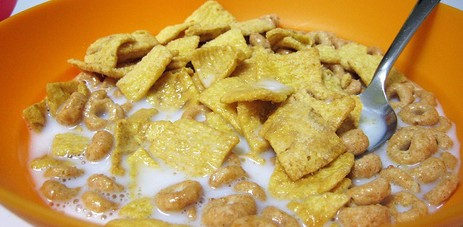
\includegraphics[width=.8\textwidth]{photos/mixtureby-dougww-flickr.jpg}\par
\textit{Prent verskaf deur dougww op Flickr.com}
\end{center}
\end{minipage}
\begin{minipage}{.5\textwidth}
\begin{figure}[H]
\label{fig:heterogeneousmixture}
\begin{center}
 \begin{pspicture}(0,-1)(11,4.7)
\SpecialCoor
\psframe[fillstyle=crosshatch*,fillcolor=white,hatchcolor=lightgray,hatchwidth=1.2pt,hatchsep=1.8pt,hatchangle=0](0,0)(4,4)
\pscircle[fillcolor=lightgray,fillstyle=solid](0.5,0.5){0.2}
\pscircle[fillcolor=white,fillstyle=solid](1,1.2){0.1}
\pscircle[fillcolor=lightgray,fillstyle=solid](2.1,1){0.2}
\pscircle[fillcolor=white,fillstyle=solid](2.3,0.4){0.1}
\pscircle[fillcolor=lightgray,fillstyle=solid](3.5,1){0.2}
\pscircle[fillcolor=white,fillstyle=solid](0.5,1.6){0.1}
\pscircle[fillcolor=white,fillstyle=solid](1,2){0.1}
\pscircle[fillcolor=white,fillstyle=solid](1.8,1.5){0.1}
\pscircle[fillcolor=lightgray,fillstyle=solid](2,2){0.2}
\pscircle[fillcolor=lightgray,fillstyle=solid](0.5,2.7){0.2}
\pscircle[fillcolor=lightgray,fillstyle=solid](2.3,2.5){0.2}
\pscircle[fillcolor=white,fillstyle=solid](2.5,2.8){0.1}
\pscircle[fillcolor=white,fillstyle=solid](3,3){0.1}
\pscircle[fillcolor=white,fillstyle=solid](3.5,2.4){0.1}
\pscircle[fillcolor=white,fillstyle=solid](0.5,3.5){0.1}
\pscircle[fillcolor=white,fillstyle=solid](2,3.4){0.1}
\pscircle[fillcolor=lightgray,fillstyle=solid](3.5,3.5){0.2}
\pscircle[fillcolor=lightgray,fillstyle=solid](1.7,3.1){0.2}
\pscircle[fillcolor=white,fillstyle=solid](3,3){0.1}
\end{pspicture}
\end{center}
\caption{ 'n Submikroskopiese voorstelling van 'n heterogene mengsel. Die grys sirkels stel een stof (bv. 'n ontbytgraan) voor en die wit sirkels stel nog 'n stof (bv. 'n ander ontbytgraan) voor. Die agtergrond is die melk.}
\end{figure}
\end{minipage}


\label{m38708*fhsst!!!underscore!!!id89}\Definition{\label{id2405839} { Heterogene mengsel }} 
{ \label{m38708*meaningfhsst!!!underscore!!!id89}
        'n Heterogene mengsel is een wat bestaan uit twee of meer stowwe, is nie-uniform en die verskillende komponente van die mengsel kan gesien word.
         } 
Heterogene mengsels kan verder onderverdeel word na gelang daarvan of dit twee vloeistowwe is wat gemeng is, 'n vaste stof en 'n vloeistof of 'n vloeistof en 'n gas of selfs 'n gas en 'n vaste stof. Vir hierdie mengsels is spesiale name gegee soos jy in die tabel hieronder sien.   \par
\begin{table}[h!]
 \begin{center}
  \begin{tabular}{|l|l|l|}\hline
   \textbf{Fases van materie} & \textbf{Naam van mengsel} & \textbf{Voorbeeld} \\ \hline
   vloeistof-vloeistof & emulsie & olie en water \\ \hline
   vaste stof-vloeistof & suspensie & modderige \\ \hline
   gas-vloeistof & a\"erosol & bruisdrankies \\ \hline
   gas-vastestof & rook & rookmis \\ \hline
  \end{tabular}

 \end{center}
\caption{Voorbeelde van verskillende heterogene mengsels}
\label{tab:mixtures}
\end{table}

      \label{m38708*uid6}
            \subsection*{Homogene mengsels}
            \nopagebreak
        \label{m38708*id62762} 'n \textbf{Homogene} mengsel het 'n definitiewe samestelling en spesifieke eienskappe. In 'n homogene mengsel kan die verskillende dele nie gesien word nie. 'n Oplossing van sout in water is 'n voorbeeld van 'n homogene mengsel. Wanneer die sout oplos, versprei dit eweredig deur die water sodat alle dele van die oplossing dieselfde is, jy kan nie meer die sout geskei van die water sien nie. Dink ook aan koffie sonder melk. Die lug wat ons inasem, is nog 'n voorbeeld van 'n homogene mengsel, want dit bestaan uit verskillende gasse wat in 'n konstante verhouding gemeng is, wat nie visueel van mekaar onderskei kan word nie (d.w.s. jy kan nie die verskillende komponente sien nie).\par 

\mindsetvid{the dissolving process}{VPabz}

\begin{minipage}{.5\textwidth}
\begin{center}
\textbf{Koffie}\\
 \includegraphics[width=.3\textwidth]{photos/coffeeby_JuliusSchorzman_wikimedia.jpg}\par
\textit{Prent verskaf deur Julius Schorzman op Wikimedia}
\end{center}
\end{minipage}
\begin{minipage}{.5\textwidth}
\begin{center}
\textbf{Sout wat oplos in water}\\
 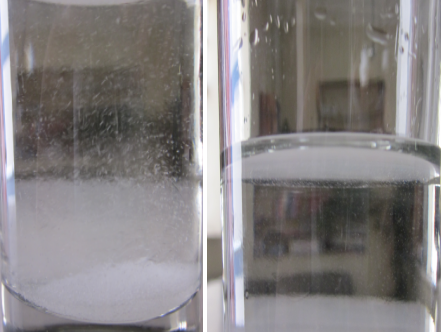
\includegraphics[width=.5\textwidth]{photos/saltwater.png}\par
\end{center}
\end{minipage}
\label{m38708*fhsst!!!underscore!!!id96}\Definition{   \label{id2405912}Homogene mengsel} { \label{m38708*meaningfhsst!!!underscore!!!id96}
        'n Homogene mengsel is een wat uniform (eenvormig) is, en waar die verskillende komponente van die mengsel nie gesien kan word nie.
         } 
%         \label{m38708*id62795}An \textbf{alloy} is a homogeneous mixture of two or more elements, at least one of which is a metal, where the resulting material has metallic properties. Alloys are usually made to improve the properties of the elements that make them up. For example steel is much stronger than iron (which is the main component of steel). Steel is a mixture (alloy) of mainly iron with carbon (to make it harder), manganese (to make it strong) and chromium (to prevent rusting).\par 

\label{m38708*eip-479}
      \begin{wex}{Mengsels}
{
\begin{minipage}{\textwidth}
Vir elk van die volgende mengsels sê of dit 'n homogene of 'n heterogene mengsel is:
\label{m38708*eip-id1167649056231}\begin{enumerate}[noitemsep, label=\textbf{\alph*}. ] 
            \leftskip=20pt\rightskip=\leftskip\item suiker opgelos in water
\item koekmeel en ystervylsels (klein stukkies yster)
% \item koekmeel en bakpoeier
% \item smarties, jellie tots en pepermente
\end{enumerate} 
\end{minipage}
}
%  \par 
%\vspace{5pt}
%\label{m38708*eip-602}\noindent\textbf{Solution to Exercise }
%\label{m38708*eip-id7325184}
{
\begin{minipage}{\textwidth}
\westep{Kyk na die definisie}
Ons kyk eers na die definisie van 'n heterogene en homogene mengsel.
\westep{Besluit of jy die komponente kan sien of nie.}
\begin{enumerate}[noitemsep, label=\textbf{\alph*}. ] 
 %           \leftskip=20pt\rightskip=\leftskip
\item Ons kan nie die suiker in die water sien nie.
\item Ons is in staat om stukkies yster in die koekmeel te sien.
% \item Daar is geen manier om te onderskei tussen die koekmeel en bakpoeier nie.
% \item Ons kan duidelik elk van die komponente waaruit die mengsel bestaan, sien. 
\end{enumerate}
\westep{Besluit of die komponente eenvormig gemeng is of nie}
\begin{enumerate}[noitemsep, label=\textbf{\alph*}. ] 
 %           \leftskip=20pt\rightskip=\leftskip
\item Die twee komponente is eenvormig gemeng.
\item In hierdie mengsel mag daar plekke wees daar baie ystervylsels is en plekke waar daar meer koekmeel is, dus is dit nie eenvormig gemeng nie.
% \item Die twee komponente van die mengsel is eenvormig gemeng.
% \item Die drie komponente van die mengsel is nie eweredig versprei nie.
\end{enumerate}
\westep{Gee die finale antwoord
}
\begin{enumerate}[noitemsep, label=\textbf{\alph*}. ] 
 %           \leftskip=20pt\rightskip=\leftskip
\item Homogene mengsel.
\item Heterogene mengsel.
% \item Homogene mengsel.
% \item Heterogene mengsel.
\end{enumerate}
\end{minipage}
}
    \end{wex}
%    \end{mdframed}
 
 %   \noindent

\begin{activity}{Die bereiding van mengsels}
{
\begin{minipage}{0.6\textwidth}
Maak mengsels van sand en water, kaliumdichromaat en water, jodium en etanol, jodium en water. Klassifiseer hierdie mengsels as heterogeen of homogeen. Gee redes vir jou keuse. Maak jou eie mengsels deur enige twee van die volgende bestanddele te gebruik \begin{itemize}[noitemsep] \item sand \item water \item klippe \item ontbytgraan \item sout \item suiker \end{itemize}Probeer om soveel verskillende mengsels as moontlik te maak. Klassifiseer elke mengsel en gee 'n rede vir jou antwoord.                                                                                                                                                                                                                                                                                                                                                                                                                       
\end{minipage}
\begin{minipage}{.4\textwidth}
{
\begin{center}
 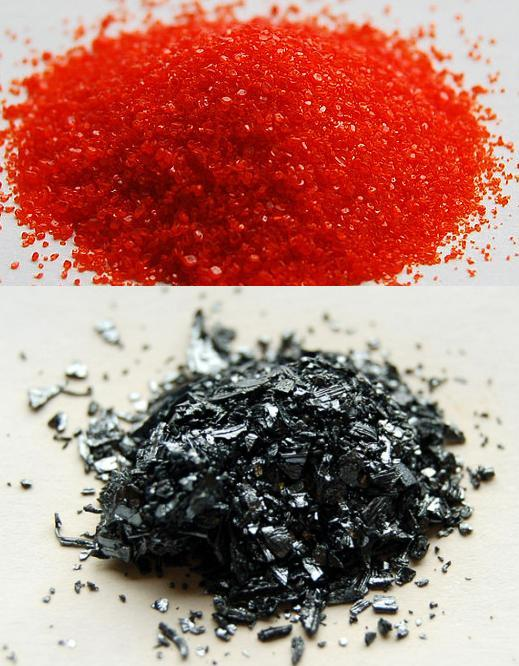
\includegraphics[width=.7\textwidth]{photos/iodine-KCr2O7-wikipedia.jpg}\par
\begin{caption}Kaliumdichromaat (bo) en jodium (onder)\end{caption}
\end{center}
}

\end{minipage}
}
\end{activity}

\begin{exercises}{Mengsels}
{Voltooi die volgende tabel: \par
%\nopagebreak
\hspace{-3cm}
\begin{tabular}{|l|p{2.5cm}|p{2.5cm}|p{2.5cm}|}\hline
\textbf{Stof} & \textbf{Nie-mengsel of} & \textbf{Heterogene} & \textbf{Homogene} \\ 
 & \textbf{mengsel} & \textbf{mengsel} & \textbf{mengsel} \\ \hline
kraanwater & & & \\ \hline
brons ( 'n allooi van koper en sink) & & & \\ \hline
beton & & & \\ \hline
aluminiumfolie & & & \\ \hline
Coca Cola & & & \\ \hline
seperige water & & & \\ \hline
swart tee & & & \\ \hline
suikerwater & & & \\ \hline
baba-melk formule & & & \\ \hline
\end{tabular}
\practiceinfo
\begin{tabular}[h]{cccccc}
 (1.) 026z  &
\end{tabular} 
}
\end{exercises}


\section{Suiwer stowwe: Elemente en verbindings}
\nopagebreak
Enige stof wat nie 'n mengsel is nie, word 'n \textbf{suiwer stof} genoem. Suiwer stowwe sluit \textbf{elemente} en \textbf{verbindings} in. Dit is baie moeiliker om suiwer stowwe in hul dele af te breek, ingewikkelde chemiese metodes is nodig om dit te doen.\par

\mindsetvid{Classifying matter}{VPacc} 

Chromatografie is die proses van die skeiding van stowwe in hul individuele komponente. As 'n stof suiwer is, sal chromatografie slegs 'n enkel stof aan die einde van die proses oplewer. As 'n stof onsuiwer is sal verskeie stowwe aan die einde van die proses sien.\par

\begin{activity}{Voorgestelde praktiese aktiwiteit: Smartie chromatografie}{
Jy benodig:
\begin{itemize}[noitemsep]
\item filtreerpapier (of kladpapier)
\item 'n paar Smarties in verskillende kleure
\item water
\item an oogdrupper
\end{itemize}
\begin{minipage}{.5\textwidth}
Plaas 'n Smartie in die middel van 'n stukkie filtreerpapier. Drup versigtig 'n paar druppels water op die Smartie, totdat die Smartie goed nat is en daar 'n ring van water op die filtreerpapier vorm. Na 'n rukkie behoort jy 'n gekleurde ring op die papier rondom die Smartie waar te neem. Dit is omdat die voedselkleursel, wat gebruik was om die Smartie te kleur, in die water opgelos het en deur die papier weg van die Smartie af beweeg het.
\end{minipage}
\begin{minipage}{.5\textwidth}
\begin{center}
 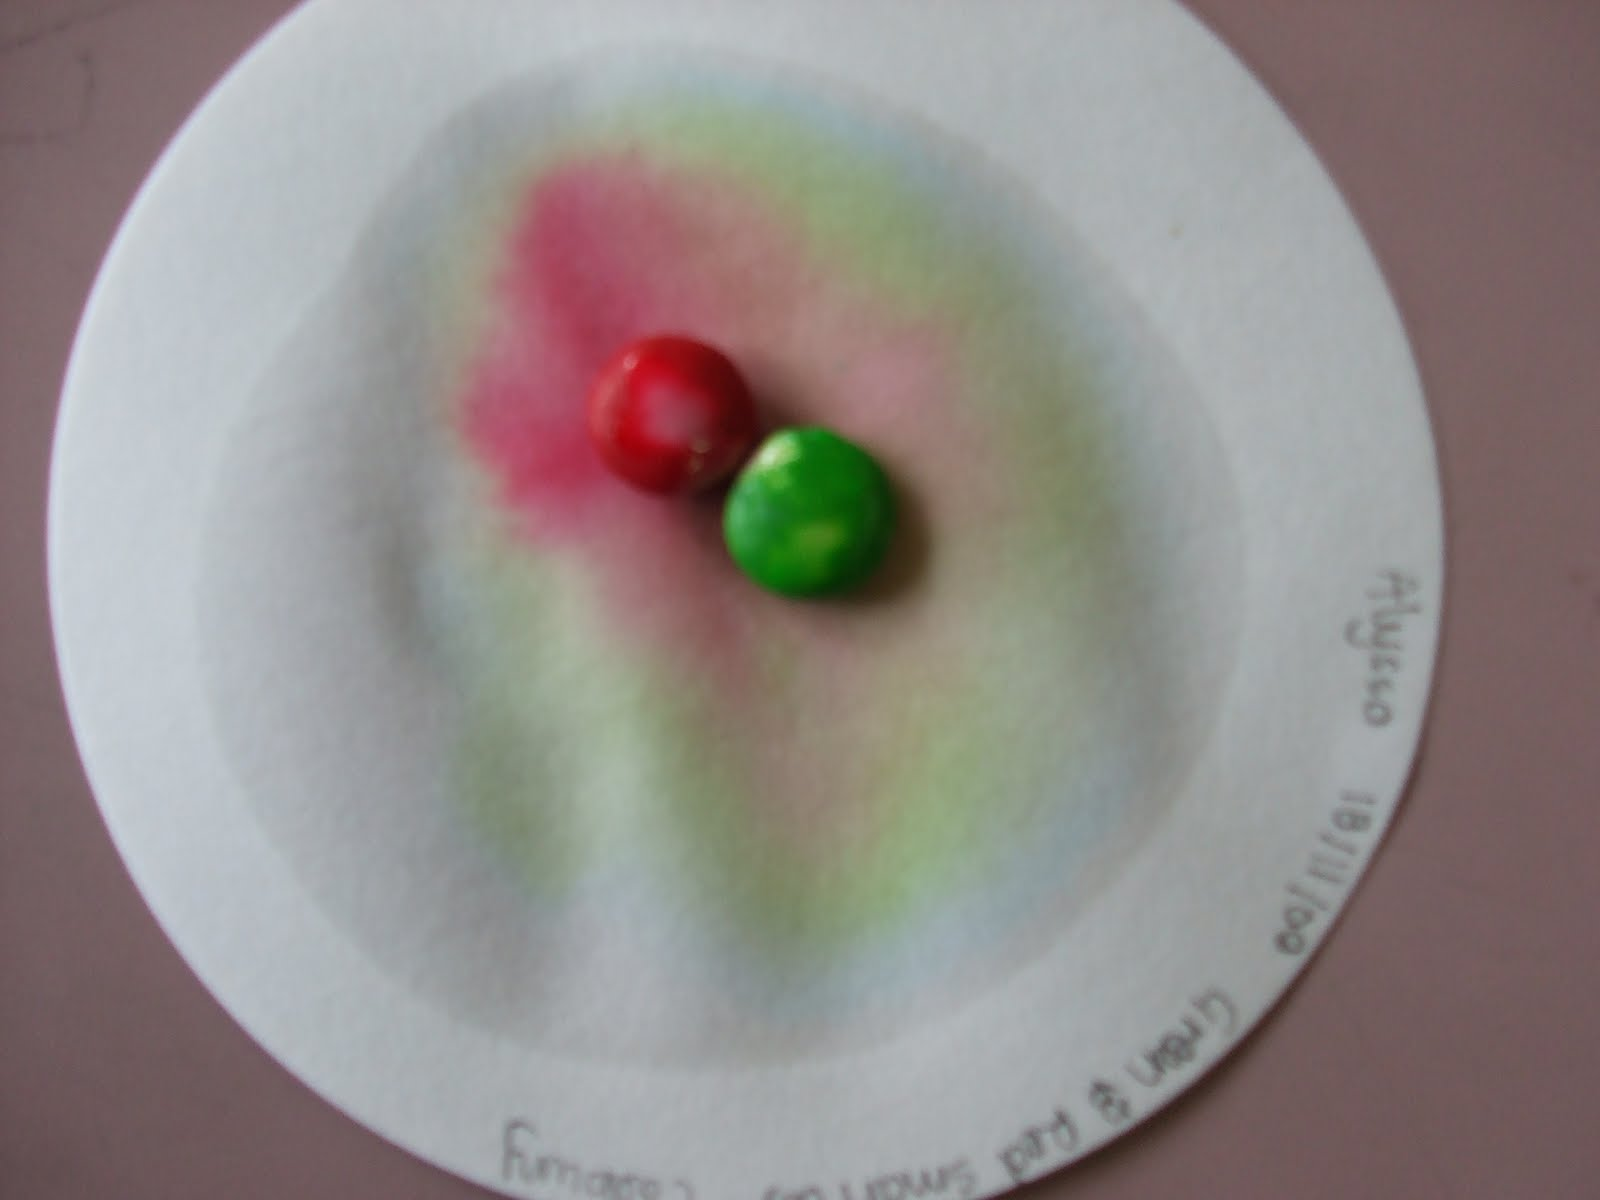
\includegraphics[width=.8\textwidth]{photos/smartie2.jpg}\par
\textit{Prent verskaf deur\\ Neil Ravenscroft - UCT}
\end{center}
\end{minipage}
}
\end{activity}
\par 
	\par
      \label{m38708*uid25}
            \subsection*{Elemente}
            \nopagebreak
        \label{m38708*id63302} 'n \textbf{Element} is 'n chemiese stof wat nie verdeel of verander kan word in ander chemiese stowwe deur gewone chemiese metodes nie. Die kleinste eenheid van 'n element is die \textbf{atoom}.\par 

\IFact{Onlangs is oor\-een\-ge\-kom dat twee by\-ko\-men\-de e\-le\-men\-te tot die amp\-te\-li\-ke lys van be\-noem\-de e\-le\-men\-te gevoeg word. Dit is e\-le\-men\-te nommers 114 en 116. Die voor\-ge\-stel\-de naam vir element 114 is flerovium en vir element 116 is dit moskovium. Dit bring die totale aantal amptelik benoemde elemente tot 114.}
\label{m38708*fhsst!!!underscore!!!id193}
\Definition{   \label{id2406278} Element } 
{ \label{m38708*meaningfhsst!!!underscore!!!id193}
 'n Element is 'n stof wat nie in ander stowwe opgebreek kan word deur chemiese metodes nie.} 
        \label{m38708*id63334}Daar is amptelik 112 benoemde elemente waarvan omtrent 118 bekende elemente is. Meeste van hierdie elemente kom natuurlik voor, maar sommige is mensgemaak. Die elemente wat ons ken word in die \textbf{Periodieke Tabel van die Elemente} voorgestel. Elke element word tot 'n \textbf{chemiese simbool} afgekort. Tabel \ref{tab:elements} gee die eerste 20 elemente en 'n paar van die algemene oorgangsmetale.\par \label{m38708*eip-775}

\begin{table}[H]
\label{tab:elements}
\begin{center}
\begin{tabular}{|l|l|l|l|}\hline
\textbf{Element naam} & \textbf{Element simbool} & \textbf{Element naam} & \textbf{Element simbool} \\ \hline
Waterstof & $\text{H}$ & Fosfor & $\text{P}$  \\ \hline
Helium & $\text{He}$ & Swawel & $\text{S}$ \\ \hline
Litium & $\text{Li}$ & Chloor & $\text{Cl}$ \\ \hline
Berillium & $\text{Be}$ & Argon & $\text{Ar}$ \\ \hline 
Boor & $\text{B}$ & Kalium & $\text{K}$ \\ \hline
Koolstof & $\text{C}$ & Kalsium & $\text{Ca}$ \\ \hline 
Stikstof & $\text{N}$ & Yster & $\text{Fe}$ \\ \hline
Suurstof & $\text{O}$ & Nikkel & $\text{Ni}$ \\ \hline 
Fluoor & $\text{F}$ & Koper & $\text{Cu}$ \\ \hline
Neon & $\text{Ne}$  & Sink & $\text{Zn}$ \\ \hline
Natrium & $\text{Na}$  & Silwer & $\text{Ag}$ \\ \hline
Magnesium & $\text{Mg}$  & Platinum & $\text{Pt}$ \\ \hline
Aluminium & $\text{Al}$ & Goud & $\text{Au}$ \\ \hline
Silikon & $\text{Si}$ & Kwik & $\text{Hg}$  \\ \hline
\end{tabular}
\end{center}
\caption{Lys van die eerste 20 elemente en 'n paar algemene oorgangsmetale}
\end{table}
\par 


      \label{m38708*uid26}
            \subsection*{Verbindings}
            \nopagebreak
        \label{m38708*id63363} 'n \textbf{Verbinding} is 'n chemiese stof wat gevorm word wanneer twee of meer verskillende elemente in 'n vaste verhouding verbind. Byvoorbeeld, Water ($\text{H}{}_{2}\text{O}$) is 'n verbinding wat bestaan uit twee waterstofatome vir elke een suurstofatoom. Natriumchloried ($\text{NaCl}$) is 'n verbinding wat bestaan uit een natriumatoom vir elke chlooratoom. 'n Belangrike eienskap van 'n verbinding is dat dit 'n \textbf{chemiese formule} het, wat die verhouding waarin die atome van elke element in die verbinding voorkom, beskryf.\par 
\label{m38708*fhsst!!!underscore!!!id201}
%\begin{definition}
%	  \begin{tabular*}{15 cm}{m{15 mm}m{}}
%	\hspace*{-50pt}  
\includegraphics[width=0.5in]{col11305.imgs/psflag2.png}   & 
\Definition{\label{id2406453} Verbinding } { \label{m38708*meaningfhsst!!!underscore!!!id201}
        'n Stof wat bestaan uit twee of meer verskillende elemente wat in 'n vaste verhouding saamgevoeg is.
         } 

\mindsetvid{Particles inside compounds}{VPacw} 

%       \end{tabular*}
%       \end{definition}
        \label{m38708*id63410} Figuur \ref{fig:classification:mixture and compound} kan jou help om die verskil tussen die terme \textbf{element}, \textbf{mengsel} en \textbf{verbinding} te verstaan. Yster ($\text{Fe}$) en swawel ($\text{S}$) is twee elemente. Wanneer hulle bymekaar gevoeg word, vorm hulle 'n \textbf{mengsel} van yster en swawel. Die yster en swawel, is nie aan mekaar verbind nie. Maar sodra die mengsel verhit word, word 'n nuwe \textbf{verbinding} gevorm, wat ystersulfied ($\text{FeS}$) genoem word.\par 
%     \setcounter{subfigure}{0}
 \begin{minipage}{.5\textwidth}
    \begin{center}
\scalebox{0.8}{
 \begin{pspicture}(0,-1)(11,4.7)
\SpecialCoor
%\psgrid[gridcolor=lightgray]
\def\fe{\pscircle[fillcolor=violet!20!gray!70!blue,fillstyle=solid](0,0){0.4}\rput(0,0){Fe}}
\def\s{\pscircle[fillcolor=yellow,fillstyle=solid](0,0){0.2}\rput(0,0){S}}
\def\fes{\fe \rput(0.6,0){\s}} 

\psframe(0,0)(4,4)
\rput(1.5,2){\s}
\rput{30}(3,1){\rput(1,1){\fe}\rput(1.5,2){\s}}
\rput{65}(1.55,1.33){\rput(1,1){\fe}\rput(1.5,2){\s}}
\rput{265}(2,3){\rput(-0.1,0.4){\fe}\rput(1.5,1.6){\s}}
\rput(2,0.6){\s}
\rput(1,1){\fe}
\rput(3,0.7){\fe}
\rput(2.4,2){\fe}
\rput(1.4,3.6){\s}
\psline(3.4,0.6)(4.2,0.6)
\uput[r](4.2,0.6){\parbox{1.5cm}{ 'n Atoom van die element yster ($\text{Fe}$)}}

\psline(3.5,3.5)(4.2,3.5)
\uput[r](4.2,3.5){\parbox{1.5cm}{ 'n Atoom van die element swawel ($\text{S}$)}}
% \rput(2,-0.5){\parbox{4cm}{A mixture of iron and sulphur}}

% \rput(7,0){
% \psframe(0,0)(4,4)
% \rput(1,2){\fes}
% \rput(1,1){\fes}
% \rput(3,0.7){\fes}
% \rput(1,3.5){\fes}
% \rput(3,3.2){\fes}
% \rput(2.4,2){\fes}
% \rput(2,-0.5){\parbox{4cm}{The compound iron sulphide (FeS)}}}

\end{pspicture}
}\\
\begin{caption} 'n Mengsel van yster en swawel\end{caption}
\label{fig:classification:mixture and compound}
    \end{center}
\end{minipage}
 \begin{minipage}{.5\textwidth}
  \begin{center}
   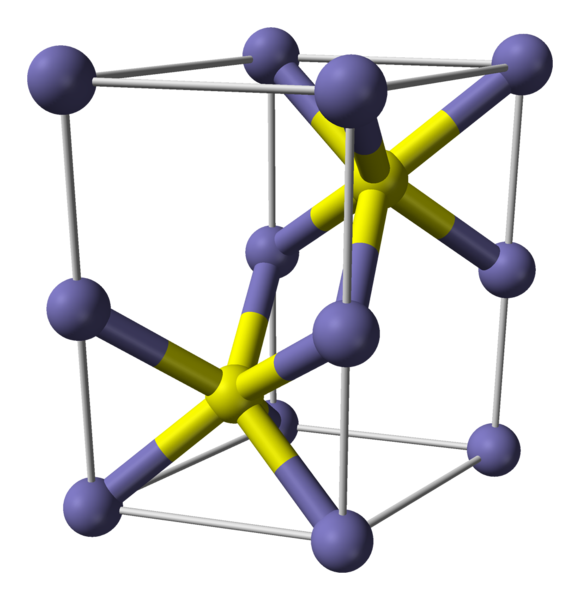
\includegraphics[width=0.4\textwidth]{photos/FeS_wikipedia.png}\\
\begin{caption} 'n Model van die ystersulfied kristal\end{caption}
  \end{center}

 \end{minipage}

\label{m38708*eip-487} Figuur \ref{fig:classification:mixture and compound} toon die submikroskopiese voorstelling van mengsels en verbindings. In 'n submikroskopiese voorstelling gebruik ons sirkels om verskillende elemente voor te stel. Om 'n verbinding te toon teken ons verskeie sirkels wat aanmekaar geheg is. Mengsels word eenvoudig as twee of meer afsonderlike elemente in dieselfde spasie aangedui. Die sirkels vir 'n mengsel is nie aanmekaar geheg nie.\par 
\label{m38708*id0124}Ons kan ook simbole gebruik om elemente, mengsels en verbindings voor te stel. Die simbole vir die elemente verskyn op die Periodieke Tabel. Verbindings word aangedui as twee of meer elementname wat reg langs mekaar geskryf word. Onderskrifte word gebruik om meer as een atoom van 'n spesifieke element aan te dui (bv. $\text{H}{}_{2}\text{O}$ of $\text{NH}_{3}$). Mengsels word geskryf as: 'n mengsel van die element (of verbinding) A en element (of verbinding) B. (bv. 'n mengsel van $\text{Fe}$ en $\text{S}$).\par 
\label{m38708*eip-524}
      \begin{wex}
{Mengsels en suiwer stowwe}
{Vir elk van die volgende stowwe stel of dit 'n suiwer stof of 'n mengsel is. As dit 'n mengsel is, is die mengsel homogeen of heterogeen? As dit 'n suiwer stof is, is dit 'n element of 'n verbinding?
\label{m38708*eip-id1167351497334}\begin{enumerate}[noitemsep, label=\textbf{\alph*}. ] 
   %         \leftskip=20pt\rightskip=\leftskip
\item Bloed (wat bestaan uit plasma en selle)
\item Argon
\item Silikondioksied ($\text{SiO}{}_{2}$)
\item Sand en klippe
\end{enumerate}
  }
%\vspace{5pt}
%\label{m38708*eip-62}\noindent\textbf{Solution to Exercise }
%\label{m38708*eip-id1167366034146}
{
\westep{Pas die definisies toe}
 'n Element word op die Periodieke Tabel gevind, so ons kyk na die Periodieke Tabel en vind dat slegs Argon daar verskyn. Vervolgens besluit ons watter is verbindings en watter is mengsels. Verbindings bestaan uit twee of meer elemente wat in 'n vaste verhouding verbind is. Sand en klippe is nie elemente nie, so ook nie bloed nie, maar silikon en suurstof is. Ten slotte besluit ons of die mengsel homogeen of heterogeen is. Aangesien ons nie die afsonderlike komponente van bloed kan sien nie is dit homogeen. Sand en klippe is heterogeen.
 %           \leftskip=20pt\rightskip=\leftskip
\westep{Skryf die antwoord neer}
\begin{enumerate}
[noitemsep, label=\textbf{\alph*}. ]
\item Bloed is 'n homogene mengsel.
\item Argon is 'n suiwer stof. Argon is 'n element.
\item Silikondioksied is 'n suiwer stof. Dit is 'n verbinding.
\item Sand en klippe vorm 'n heterogene mengsel.
\end{enumerate}}
    \end{wex}


  \label{m38708*eip-326}
\begin{activity}{Die gebruik van modelle om stowwe te verteenwoordig}{
\begin{minipage}{.5\textwidth}
Die volgende stowwe word gegee:
\label{m38708*eip-id1166921187210}
\begin{itemize}[noitemsep]
\item Lug (bestaande uit suurstof, stikstof, waterstof, waterdamp)
\item Waterstofgas ($\text{H}_{2}$)
\item Neongas
\item Stoom
\item Ammoniakgas ($\text{NH}_{3}$)
\end{itemize}
\end{minipage}
\begin{minipage}{.5\textwidth}
\begin{center}
 \includegraphics[width=.8\textwidth]{photos/models_classification.jpg}\par
\end{center}
\end{minipage}
\noindent
\begin{enumerate}[noitemsep, label=\textbf{\arabic*}.]
\item Gebruik gekleurde balle om modelle te bou vir elk van die stowwe wat gegee is.
\item Klassifiseer die stowwe as: elemente, verbindings, homogene mengsels, heterogene mengsel, suiwer stof, onsuiwer stof.
\item Teken submikroskopiese voorstelling vir elk van die bogenoemde voorbeelde.
\end{enumerate}

}
\end{activity}
%NTS add image here 
\par \label{m38708*secfhsst!!!underscore!!!id212}
            \begin{exercises}{Elemente, mengsels en verbindings}{
            \nopagebreak
            \label{m38708*id63472}
 \begin{enumerate}[noitemsep, label=\textbf{\arabic*}. ] 
            \label{m38708*uid28}
    \item Merk in die volgende tabel watter van die gegewe stowwe 'n \textsl{mengsel} of 'n \textsl{suiwer stof} is. As dit 'n mengsel is, sê ook of die mengsel homogeen of heterogeen is.
    % \textbf{m38708*id63499}\par
          \begin{table}[H]
    % \begin{table}[H]
    % \\ 'id2876023' '1'
        \begin{center}
      \label{m38708*id63499}
    \noindent
      \begin{tabular}{|l|l|l|}\hline
        \textbf{Stof} &
        \textbf{Mengsel of suiwer} &
        \textbf{Homogene of heterogene mengsel} \\ \hline
        bruis koeldrank & & \\ \hline
        staal & & \\ \hline
        suurstof & & \\ \hline
        ystervylsels & & \\ \hline
        rook & & \\ \hline
        kalksteen (${\text{CaCO}}_{3}$) & & \\ \hline
    \end{tabular}
      \end{center}
%    \begin{center}{\small\bfseries Table 1.1}\end{center}
%    \begin{caption}{\small\bfseries Table 1.1}\end{caption}
\end{table}
    \par
\label{m38708*uid29}\item In elk van die volgende gevalle, sê of die stof 'n element, 'n mengsel of 'n verbinding is.
\label{m38708*id63912}\begin{enumerate}[noitemsep, label=\textbf{\alph*}. ] 
            \label{m38708*uid30}\item $\text{Cu}$
\label{m38708*uid31}\item yster en swawel
\label{m38708*uid32}\item $\text{Al}$
\label{m38708*uid33}\item $\text{H}{}_{2}\text{SO}{}_{4}$
\label{m38708*uid34}\item $\text{SO}{}_{3}$\end{enumerate}
                \end{enumerate}

\practiceinfo
\begin{tabular}[h]{cccccc}
 (1.) 0270  &  (2.) 0271  & 
\end{tabular}
}
\end{exercises}
%NTS DIAGRAM is needed here and some more examples in the above exercises
            \section{Gee name en formules aan stowwe}
            \nopagebreak
      \label{m38708*eip-379}Dink na oor wat jy jou vriende noem. Sommige van jou vriende mag volle name (lang name) en 'n bynaam (kort naam) hê. Dit is die woorde wat ons gebruik om ander te vertel na wie of wat ons verwys. Hulle volle naam is soos die stowwe se naam; en hulle bynaam is soos stowwe se formules. Sonder hierdie name het jou vriende geen idee na wie van hulle jy verwys nie. Chemiese stowwe het name, net soos mense name het. Dit help wetenskaplikes om doeltreffend te kommunikeer. 
     \par \label{m38708*id64028}Dit is maklik om elemente en mengsels te beskryf. Ons gebruik eenvoudig die name wat ons op die Periodieke Tabel van elemente kry en gebruik woorde om mengsels te beskryf. Maar hoe word verbindings benoem? In die voorbeeld van ystersulfied wat vroeër gebruik is, is die saamgestelde naam 'n kombinasie van die name van die elemente, maar effens verander. \par 

\mindsetvid{why do chemical compounds form}{VPadm} 

      \label{m38708*id64033}Die volgende is 'n paar riglyne vir die benaming van verbindings:\par 
      \label{m38708*id64037}\begin{enumerate}[noitemsep, label=\textbf{\arabic*}. ] 
            \label{m38708*uid35}\item Die verbinding se naam sal altyd die \textbf{name van die elemente} wat deel daarvan vorm insluit.
\label{m38708*id64059}\begin{itemize}[noitemsep]
            \label{m38708*uid36}\item 'n Verbinding van \textbf{yster} ($\text{Fe}$) en \textsl{swawel} ($\text{S}$) is \textbf{yster}\textsl{sulf}ied ($\text{FeS}$)
\label{m38708*uid37}\item 'n Verbinding van \textbf{kalium} ($\text{K}$) en \textsl{broom} ($\text{Br}$) is \textbf{kalium}\textsl{brom}ied ($\text{KBr}$)
\label{m38708*uid38}\item 'n Verbinding van \textbf{natrium} ($\text{Na}$) and \textsl{chloor} ($\text{Cl}$) is \textbf{natrium}\textsl{chlor}ied ($\text{NaCl}$)
\end{itemize}
        \label{m38708*uid39}\item In 'n verbinding, word die element aan die linkerkant van die Periodieke Tabel \textsl{eerste} gebruik by die benoeming van die verbinding. In die voorbeeld van $\text{NaCl}$, is natrium 'n groep 1 element op die linkerkant van die tabel, terwyl chloor in Groep 7 is aan die regterkant van die tabel. Natrium kom dus eerste in die verbinding se naam voor. Dieselfde geld vir $\text{FeS}$ en $\text{KBr}$.
\label{m38708*uid40}\item Die \textbf{simbole} van die elemente kan gebruik word om verbindings voor te stel, bv. $\text{FeS}$, $\text{NaCl}$, $\text{KBr}$ en $\text{H}{}_{2}\text{O}$. Dit word die chemiese formules genoem. In die eerste drie voorbeelde, is die verhouding van die elemente in elke verbinding 1:1. Dus is daar een atoom yster vir elke swawel atoom in die verbinding. In die laaste voorbeeld ($\text{H}{}_{2}\text{O}$) is daar twee atome waterstof vir elke atoom suurstof in die verbinding.
\item 'n Verbinding kan \textbf{ione} ( 'n ioon is 'n atoom wat elektrone verloor of bygekry het) bevat. Hierdie ione kan enkelvoudig (bestaan uit net een element) of meervoudig (bestaan uit verskeie elemente) wees. Sommige van die meer algemene ione en hul formules word in tabel \ref{tab:cations} en tabel \ref{tab:anions} gegee. Jy behoort al hierdie ione te ken.

    % \textbf{m38708*id64235}\par
    %      \begin{table}[H]
    % \begin{table}[H]
    % \\ 'id2876536' '1'

\begin{table}[H]
\begin{center}
\label{tab:cations}
\begin{tabular}{|l|c|l|c|l|c|l|c|} \hline
\textbf{Ioonverbinding} & \textbf{Formule} & \textbf{Ioonverbinding} & \textbf{Formule} & \textbf{Ioonverbinding} & \textbf{Formule}  \\ \hline
Waterstof       & $\text{H}^{+}$   & Litium          & $\text{Li}^{+}$     & Natrium          & $\text{Na}^{+}$  \\ \hline
Kalium          & $\text{K}^{+}$   & Silwer          & $\text{Ag}^{+}$     & Kwikk (I)        & $\text{Hg}^{+}$  \\ \hline
Koper (I)       & $\text{Cu}^{+}$  & Ammonium        & $\text{NH}_{4}^{+}$ & Berillium        & $\text{Be}^{2+}$ \\ \hline
Magnesium       & $\text{Mg}^{2+}$ & Kalsium         & $\text{Ca}^{2+}$    & Barium           & $\text{Ba}^{2+}$ \\ \hline
Tin (II)        & $\text{Sn}^{2+}$ & Lood (II)       & $\text{Pb}^{2+}$    & Chroom (II)      & $\text{Cr}^{2+}$ \\ \hline
Mangaan (II)    & $\text{Mn}^{2+}$ & Yster (II)      & $\text{Fe}^{2+}$    & Kobalt (II)      & $\text{Co}^{2+}$ \\ \hline
Nikkel          & $\text{Ni}^{2+}$ & Koper (II)      & $\text{Cu}^{2+}$    & Sink             & $\text{Zn}^{2+}$ \\ \hline
Aluminium       & $\text{Al}^{3+}$ & Chroom (III)    & $\text{Cr}^{3+}$    & Yster (III)      & $\text{Fe}^{3+}$ \\ \hline
Kobalt (III)    & $\text{Co}^{3+}$ & Chroom (VI)     & $\text{Cr}^{6+}$    & Mangaan (VII)    & $\text{Mn}^{7+}$ \\ \hline

\end{tabular}

 \end{center}
\caption{Tabel van katione}
\label{tab:cations}
\end{table}

\begin{table}[H]
\begin{center}
\label{tab:anions}
\begin{tabular}{|l|c|l|c|l|c|l|c|} \hline
\textbf{Ioonverbinding} & \textbf{Formule}            & \textbf{Ioonverbinding} & \textbf{Formule} \\ \hline
Fluoried                & $\text{F}^{-}$             & Oxied               & $\text{O}^{2-}$ \\ \hline
Chloried                & $\text{Cl}^{-}$            & Peroksied           & $\text{O}_{2}^{2-}$ \\ \hline
Bromied                 & $\text{Br}^{-}$            & Karbonaat           & $\text{CO}_{3}^{2-}$ \\ \hline
Jodied                  & $\text{I}^{-}$             & Sulfied             & $\text{S}^{2-}$ \\ \hline
Hidroksied              & $\text{OH}^{-}$            & Sulfiet             & $\text{SO}_{3}^{2-}$ \\ \hline
Nitriet                 & $\text{NO}_{2}^{-}$        & Sulfaat             & $\text{SO}_{4}^{2-}$ \\ \hline
Nitraat                 & $\text{NO}_{3}^{-}$        & Thiosulfaat         & $\text{S}_{2}{\text{O}}_{3}^{2-}$ \\ \hline
Waterstofkarbonaat      & $\text{HCO}_{3}^{-}$       & Chromaat            & $\text{CrO}_{4}^{2-}$ \\ \hline
Waterstofsulfiet        & $\text{HSO}_{3}^{-}$       & Dichromaat          & $\text{Cr}_{2}{\text{O}}_{7}^{2-}$ \\ \hline
Waterstofsulfaat        & $\text{HSO}_{4}^{-}$       & Manganaat           & $\text{MnO}_{4}^{2-}$ \\ \hline
Diwaterstoffosfaat      & $\text{H}_{2}{\text{PO}}_{4}^{-}$ & Oksalaat     & $\text{(COO)}_{2}^{2-}/{\text{C}}_{2}{\text{O}}_{4}^{2-}$ \\ \hline
Hipochloriet            & $\text{ClO}^{-}$           & Waterstoffosfaat    & $\text{HPO}_{4}^{2-}$ \\ \hline
Chloraat                & $\text{ClO}_{3}^{-}$       & Nitried             & $\text{N}^{3-}$ \\ \hline
Permanganaat            & $\text{MnO}_{4}^{-}$       & Fosfaat             & $\text{PO}_{4}^{3-}$ \\ \hline
Asetaat Etanoaat        & $\text{CH}_{3}{\text{COO}}^{-}$   & Fosfied      & $\text{P}^{3-}$ \\ \hline
\end{tabular}

 \end{center}
\caption{Tabel van anione}
\label{tab:anions}
\end{table}

    \par
  \label{m38708*uid42}\item Wanneer daar slegs twee elemente in die verbinding is, kry die verbinding dikwels die \textbf{agtervoegsel} (op die end) \textbf{–ied}. Jy sou dit reeds opgelet het in sommige van die voorbeelde wat ons tot dusver gebruik het. Vir saamgestelde ione, wanneer 'n nie-metaal met suurstof verbind om 'n negatiewe ioon (anioon) te vorm wat dan weer met 'n positiewe ioon (katioon) soos waterstof of 'n metaal verbind, is die agtervoegsel van die naam \textbf{–aat} of \textbf{–iet}. By voorbeeld, $\text{NO}_{3}^{-}$ is 'n negatiewe ioon, wat kan verbind met 'n katioon soos waterstof ($\text{HNO}{}_{3}$) of 'n metaal soos kalium ($\text{KNO}{}_{3}$). Die $\text{NO}_{3}^{-}$ anioon het die naam nitr\textbf{aat}. $\text{SO}_{3}^{2-}$ in 'n formule is sulf\textbf{iet}, bv. natriumsulf\textbf{iet} ($\text{Na}{}_{2}\text{SO}{}_{3}$). $\text{SO}_{4}^{2-}$ is sulf\textbf{aat} en $\text{PO}_{4}^{3-}$ is fosf\textbf{aat}.
\label{m38708*uid43}\item \textbf{Voorvoegsels} kan gebruik word om die verhouding van die elemente in die verbinding te beskryf. Dit word vir nie-metale gebruik. Vir metale, voeg ons 'n romeinse syfer (I, II, III, IV) in hakies na die metaalioon om die verhouding aan te dui. Jy behoort die volgende voorvoegsels te ken: "mono" (een), "di" (twee) en 'tri " (drie).
\label{m38708*id64977}\begin{itemize}[noitemsep]
            \label{m38708*uid44}\item $\text{CO}$ (koolstof\textbf{mon}oksied) - Daar is een suurstof atoom suurstof vir elke een koolstof atoom
\label{m38708*uid45}\item $\text{NO}{}_{2}$ (stikstof\textbf{di}oksied) - Daar is twee suurstof atome vir elke een stikstof atoom
\label{m38708*uid46}\item $\text{SO}{}_{3}$ (swawel \textbf{tri}oksied) - Daar is drie suurstof atome vir elke een swawel atoom
\end{itemize}
        \end{enumerate}
\label{m38708*id537402}Bogenoemde riglyne help ons ook om vanaf die naam van die verbinding die formule van 'n verbinding uit te werk.\par 
\label{m38708*eip-178}Wanneer die formule van 'n verbinding uitgewerk word, werk ons terugwaarts. By voorbeeld, as jy gevra word om die formule van kaliumchloried te gee, begin deur daarop te let dat ons kalium en chloried het. Skryf vervolgens die formule neer vir elk van hierdie ione. Kalium is ${\text{K}}^{+}$ en chloried is ${\text{Cl}}^{-}$. Die finale stap is om te let op die lading op elke ioon en te kyk hoe die ladings kombineer. Aangesien beide kalium en chloor 'n lading van 1 het, verbind hulle in 'n 1:1 verhouding. Die formule is $\text{KCl}$.\par \label{m38708*notfhsst!!!underscore!!!id252}
%\begin{tabular}{cc}
%	   \hspace*{-50pt}\raisebox{-8 mm}{ 
\includegraphics[width=0.5in]{col11305.imgs/pstip2.png}  }& 
%	\begin{minipage}{0.85\textwidth}
%	\begin{note}
\Tip{Wanneer getalle as onderskrifte in verbindings (dit wil sê hulle word onder en aan die regterkant van die element se simbool geskryf) geskryf word, sê dit vir ons hoeveel atome van daardie element daar is in verhouding tot die ander elemente in die verbinding. Byvoorbeeld in stikstofdioksied (${\text{NO}}_{2}$) is daar twee suurstof atome vir elke een stikstof atoom. Later, wanneer ons begin kyk na chemiese vergelykings, sal jy agterkom dat daar somtyds nommers \textbf{voor} die naam van die verbindings is. So beteken $2\text{H}{}_{2}\text{O}$, byvoorbeeld, dat daar twee molekules water is en dat daar in elke molekule twee waterstofatome vir elke een suurstof atoom is.\par}  
%	\end{note}
%	\end{minipage}
%	\end{tabular}
	\par
\label{m38708*eip-163}Ons kan hierdie reëls gebruik om ons te help met die naam van beide ioniese verbindings en kovalente verbindings. Wetenskaplikes gee egter dikwels ander name vir kovalente verbindings om die naam te vereenvoudig (of omdat die molekuul benoem was lank voordat die formule ontdek is). Byvoorbeeld, as ons 2 waterstofatome en 1 suurstofatoom het, sal volgens bogenoemde benamingsreëls die naam van die stof diwaterstofmonoksied wees. Maar hierdie verbinding is beter bekend as water!  \par \label{m38708*eip-254} 

\begin{wex}{Skryf die chemiese formules 1}
{Wat is die formule vir natriumfluoried? }
{\westep {Noem die ione wat betrokke is:}
Ons het die natriumioon ($\text{Na}^{+}$) en die fluoriedioon ($\text{Fl}^{-}$). (Jy kan dit op die tabelle van anione en katione naslaan.)
\westep{Skryf die ladings van die ione neer:}
Natrium het 'n lading van $+1$ en fluoor het 'n lading van $-1$.
\westep{Vind die regte kombinasie:}
Vir elke plus moet daar 'n minus wees. Dus benodig die $+1$ natriumioon een $-1$ fluoriedioon sodat die lading gebalanseer is. Natrium en fluor verbind in 'n 1:1 verhouding.
\westep{Skryf die formule neer:}
$\text{NaFl}$
}
\end{wex}
      \begin{wex}{Skryf die chemiese formules 2}
{Wat is die formule vir magnesiumchloried? }
{\westep {Noem die ione wat betrokke is:}
Ons het die magnesiumioon ($\text{Mg}^{2+}$) en die chloriedioon ($\text{Cl}^{-}$).
\westep{Skryf die ladings van die ione neer:}
Magnesium het 'n lading van $+2$ en chloor het 'n lading van $-1$.
\westep{Vind die regte kombinasie:}
Vir elke plus moet daar 'n minus wees. Dus benodig die $+2$ magnesiumioon twee $-1$ chloriedione sodat die lading gebalanseer is. Magnesium en chloor verbind in 'n 1:2 verhouding. Daar is 'n eenvoudige manier om hierdie verhouding te bepaal:
\begin{figure}[H] % horizontal\label{m38708*uid27}
    \begin{center}
 \begin{pspicture}(0,0)(2,2)
\SpecialCoor
\psline[linewidth=0.04]{->}(0,1)(1,0)
\uput[r](-1.2,1){\large{$\text{Mg}^{2+}$}}
\psline[linewidth=0.04]{->}(0,0)(1,1)
\uput[r](-1,0){\large{$\text{Cl}^{-}$}}
\uput[r](1,1){\large{$2$}}
\uput[r](1,0){\large{$1$}}

\end{pspicture}
\end{center}
\end{figure}
Teken 'n kruis soos bo aangedui en kyk dan hoe $\text{Mg} \rightarrow 1$ en $\text{Cl} \rightarrow 2$. 
\westep{Skryf die formule neer:}
$\text{MgCl}{}_{2}$
}
\end{wex} 

    
    \noindent

      \noindent
      \begin{wex}{Skryf die chemiese formules 3}
{Wat is die formule vir magnesiumoksied? }
{\westep {Noem die ione wat betrokke is:}
Ons het die magnesiumioon ($\text{Mg}^{2+}$) en die chloriedioon ($\text{O}^{2-}$).
\westep{Vind die regte kombinasie:}
$\text{Mg}^{2+} : 2$ \newline
$\text{O}^{2-} : 2$ \newline
As jy die kruismetode gebruik, sal jy 'n verhouding van $2:2$ kry. Hierdie verhouding moet altyd in sy eenvoudigste vorm gegee word, m.a.w. $1:1$.
\westep{Skryf die formule neer:}
$\text{MgO}$
}
\end{wex}

      \begin{wex}{Skryf die chemiese formules 4}
{Wat is die formule vir koper(II)nitraat? }
{\westep {Noem die ione wat betrokke is:}
$\text{Cu}^{2+}$ (die vraag s\^e koper(II), nie koper(I) nie) \newline
$\text{NO}_{3}^{-}$
\westep{Vind die regte kombinasie:}
	\begin{figure}[H] % horizontal\label{m38708*uid27}
    \begin{center}
 \begin{pspicture}(0,0)(2,2)
\SpecialCoor
\psline[linewidth=0.04]{->}(0,1)(1,0)
\uput[r](-1,1){\large{$\text{Cu}^{2+}$}}
\psline[linewidth=0.04]{->}(0,0)(1,1)
\uput[r](-1.2,0){\large{$\text{NO}_{3}^{-}$}}
\uput[r](1,1){\large{$2$}}
\uput[r](1,0){\large{$1$}}

\end{pspicture}
\end{center}
\end{figure}
\westep{Skryf die formule neer:}
${\text{Cu}}({\text{NO}}_{3})_{2}$
}
\end{wex}

\Tip{Let op hoe ons in die laaste voorbeeld $\text{NO}_{3}^{-}$ binne die hakies geskryf het. Ons doen dit om aan te dui dat $\text{NO}_{3}^{-}$ 'n saamgestelde ioon is en dat daar twee van hierdie ione aan een koperioon verbind is.}

\begin{activity}{Die ioon-maat-soek speletjie}
Jou onderwyser sal aan elkeen van julle 'n ander ioon toeken (geskryf op 'n kaartjie). Plak dit op jou. Jy sal ook kaarte kry met die syfers 1 - 5 op. Loop nou in die klas rond en soek  'n maat, hou in gedagte watter ioon by jou kan pas en in watter verhouding. Sodra jy 'n maat gevind het, gee  'n aanduiding van die verhouding van elke ioon deur die genommerde kaarte te gebruik. Kontroleer jou resultate met jou klasmaats of jou onderwyser.
\end{activity}

  \label{m38708*secfhsst!!!underscore!!!id255}
            \begin{exercises}{Name van Verbindings}
{            \nopagebreak \noindent
      \label{m38708*id65118}\begin{enumerate}[noitemsep, label=\textbf{\arabic*}. ] 
            \label{m38708*uid47}\item Die formule vir kalsiumkarbonaat $\text{CaCO}{}_{3}$.
\label{m38708*id65148}\begin{enumerate}[noitemsep, label=\textbf{\alph*}. ] 
            \label{m38708*uid48}\item Is kalsiumkarbonaat 'n element of 'n verbinding? Gee 'n rede vir jou antwoord.
\label{m38708*uid49}\item Wat is die verhouding van $\text{Ca}:\text{C}:\text{O}$ atome in die formule?
\end{enumerate}
\label{m38708*uid50}\item Gee die naam van elk van die volgende stowwe.
\label{m38708*id65189}\begin{enumerate}[noitemsep, label=\textbf{\alph*}. ] 
            \label{m38708*uid51}\item $\text{KBr}$
\label{m38708*uid52}\item $\text{HCl}$
\label{m38708*uid53}\item ${\text{KMnO}}_{4}$\label{m38708*uid54}\item ${\text{NO}}_{2}$\label{m38708*uid55}\item ${\text{NH}}_{4}\text{OH}$
\label{m38708*uid56}\item ${\text{Na}}_{2}{\text{SO}}_{4}$
\item ${\text{Fe}}({\text{NO}}_{3})_3$
\item ${\text{Pb}}{\text{SO}}_{3}$
\item ${\text{Cu}}({\text{HCO}}_{3})_2$
\end{enumerate}
\label{m38708*uid57}\item Gee die chemiese formule vir elk van die volgende verbindings.
\label{m38708*id65338}\begin{enumerate}[noitemsep, label=\textbf{\alph*}. ] 
            \label{m38708*uid58}\item Kaliumnitraat
\label{m38708*uid59}\item Natriumoksied
\label{m38708*uid60}\item Bariumsulfaat
\label{m38708*uid61}\item Aluminiumchloried
\label{m38708*uid62}\item Magnesiumfosfaat
\item Tin(II)bromied
\item Mangaan(II)fosfied
\end{enumerate}
\end{enumerate}

\practiceinfo
\begin{tabular}[h]{cccccc}
 (1.) 0272  &  (2.) 0273  &  (3.) 0274   & & 
\end{tabular}
}
\end{exercises}
%The above exercise needs more examples and some diagrams! Possibly also lost a curly brace
            \section{Metale, Metallo\"ide en Nie-metale}
%ADD a simple periodic table here to show this
            \nopagebreak
      \label{m38708*id65693}Die elemente in die Periodieke Tabel kan ook op grond van hulle eienskappe verdeel word as \textbf{metale}, \textbf{metallo\"ide} of \textbf{nie-metale}. Die sigsaglyn (zigzag) skei al die metaalelemente van die nie-metale. Metale word aan die linkerkant van die lyn gevind, en die nie-metale is aan die regterkant. Langs die lyn vind jy die metalloïde. Jy behoort daarop te let dat daar meer metale as nie-metale is. Metale, metallo\"ide en nie-metale het almal hul eie spesifieke eienskappe.\par 

\mindsetvid{classifying matter}{VPaec} 

\begin{figure}[h]

\begin{center}
\scalebox{0.7}{
\begin{pspicture}(-2,-2)(20,10)
%\psgrid[gridcolor=gray]
\psset{unit=1}
\pspolygon[fillstyle=solid,fillcolor=teal!20!white](0,3)(0,4)(1,4)(1,3)(0,3)
\pspolygon[fillstyle=solid,fillcolor=lightgray](0,-1)(0,3)(2,3)(2,1)(12,1)(12,2)(13,2)(13,0)(14,0)(14,-1)(0,-1)
\pspolygon[fillstyle=solid,fillcolor=cyan!50!white](12,2)(12,3)(13,3)(13,2)(12,2)
\pspolygon[fillstyle=solid,fillcolor=cyan!50!white](13,0)(13,2)(14,2)(14,1)(15,1)(15,0)(16,0)(16,-1)(14,-1)(14,0)(13,0)
\pspolygon[fillstyle=solid,fillcolor=teal!20!white](14,2)(13,2)(13,3)(17,3)(17,4)(18,4)(18,-1)(16,-1)(16,0)(15,0)(15,1)(14,1)(14,2)
\uput[l](4,0){\Huge{Metale}}
\uput[l](15.1,0.5){\LARGE{Metallo\"ide}}
\uput[l](13.1,2.5){\Large{Metallo\"ide}}
\uput[l](17.6,1.8){\Huge{Nie-metale}}
\uput[l](0.9,3.5){\Huge{H}}
\end{pspicture}
}
\end{center}
\caption{'n Vereenvoudigde diagram wat  'n gedeelte van die Periodieke Tabel aantoon.}
\label{fig:periodic}
\end{figure} 
      \label{m38708*uid76}
            \subsection*{Metale}
            \nopagebreak
\begin{minipage}{.5\textwidth}
        \label{m38708*id65726}Voorbeelde van metale sluit in koper ($\text{Cu}$), sink ($\text{Zn}$), goud ($\text{Au}$), silwer ($\text{Ag}$), tin ($\text{Sn}$) en lood ($\text{Pb}$). Die volgende is sommige van die eienskappe van metale:\par 
\end{minipage}
\begin{minipage}{.5\textwidth}
\begin{center}
\textbf{Koperdraad}\\
 \includegraphics[width=.2\textwidth]{photos/copperwire.jpg}
\end{center}
\end{minipage}

        \label{m38708*id65732}\begin{itemize}[noitemsep]
            \label{m38708*uid77}\item \textsl{Termiese geleiers} \\
       Metale is goeie geleiers van hitte en word dus gebruik in kombuis gereedskap soos potte en panne.
\label{m38708*uid78}\item \textsl{Elektriese geleiers} \\
       Metale is goeie geleiers van elektrisiteit en word dus gebruik in elektriese geleidingsdrade.
\label{m38708*uid79}\item \textsl{Blink metaalglans} \\
       Metale het 'n kenmerkende blink voorkoms en word dikwels gebruik om juweliersware te maak.
\label{m38708*uid80}\item \textsl{Smeebaar en pletbaar} \\
       Dit beteken dat hulle kan in  'n vorm gebuig word sonder om te breek (smeebaar) en kan uitgerek word in dun drade
      (rekbaar) soos koper.
\label{m38708*uid81}\item \textsl{Smeltpunt} \\
       Metale het gewoonlik 'n hoë smeltpunt en kan dus gebruik word om kookpotte te maak 
      en ander toerusting wat baie warm kan word, sonder om te beskadig.
\label{m38708*uid82}\item \textsl{Digtheid} \\
       Metale het 'n hoë digtheid.
\item \textsl{Magnetiese eienskappe} \\ 
       Slegs drie hoofmetale (yster, kobalt en nikkel) is magneties, die ander is nie-magneties.
\end{itemize}
         \label{m38708*id65852}Dit hoort duidelik te wees hoe die eienskappe van metale hul baie nuttig maak vir sekere doeleindes.\par 
\label{m38708*secfhsst!!!underscore!!!id320} 
            \begin{activity}{Groep Werk : 1. Kyk na metale}{
            \nopagebreak
\begin{minipage}{0.5\textwidth}
        \label{m38708*id65869}\begin{enumerate}[noitemsep, label=\textbf{\arabic*}. ]
            \label{m38708*uid83}\item Versamel 'n paar metaal-items by jou huis of skool. Hieronder is  'n paar voorbeelde:
\label{m38708*id65885}\begin{itemize}[noitemsep]
            \label{m38708*uid84}\item haarknippies
\label{m38708*uid85}\item haakspelde
\label{m38708*uid86}\item kookpotte
\label{m38708*uid87}\item juwele
\label{m38708*uid88}\item sk\^er
\label{m38708*uid89}\item eetgerei (messe, vurke, lepels)
\end{itemize}
        \label{m38708*uid90}\item In groepe van 3-4, voeg jou versameling metaal voorwerpe by die ander.
\label{m38708*uid91}\item Wat is die funksie van elk van hierdie voorwerpe?
\label{m38708*uid92}\item Bespreek waarom jy dink metaal is gebruik om elk van die voorwerpe te maak. Oorweeg die eienskappe van metale wanneer jy hierdie vraag beantwoord. 
\end{enumerate}
\end{minipage}
\begin{minipage}{.5\textwidth}
\begin{center}
 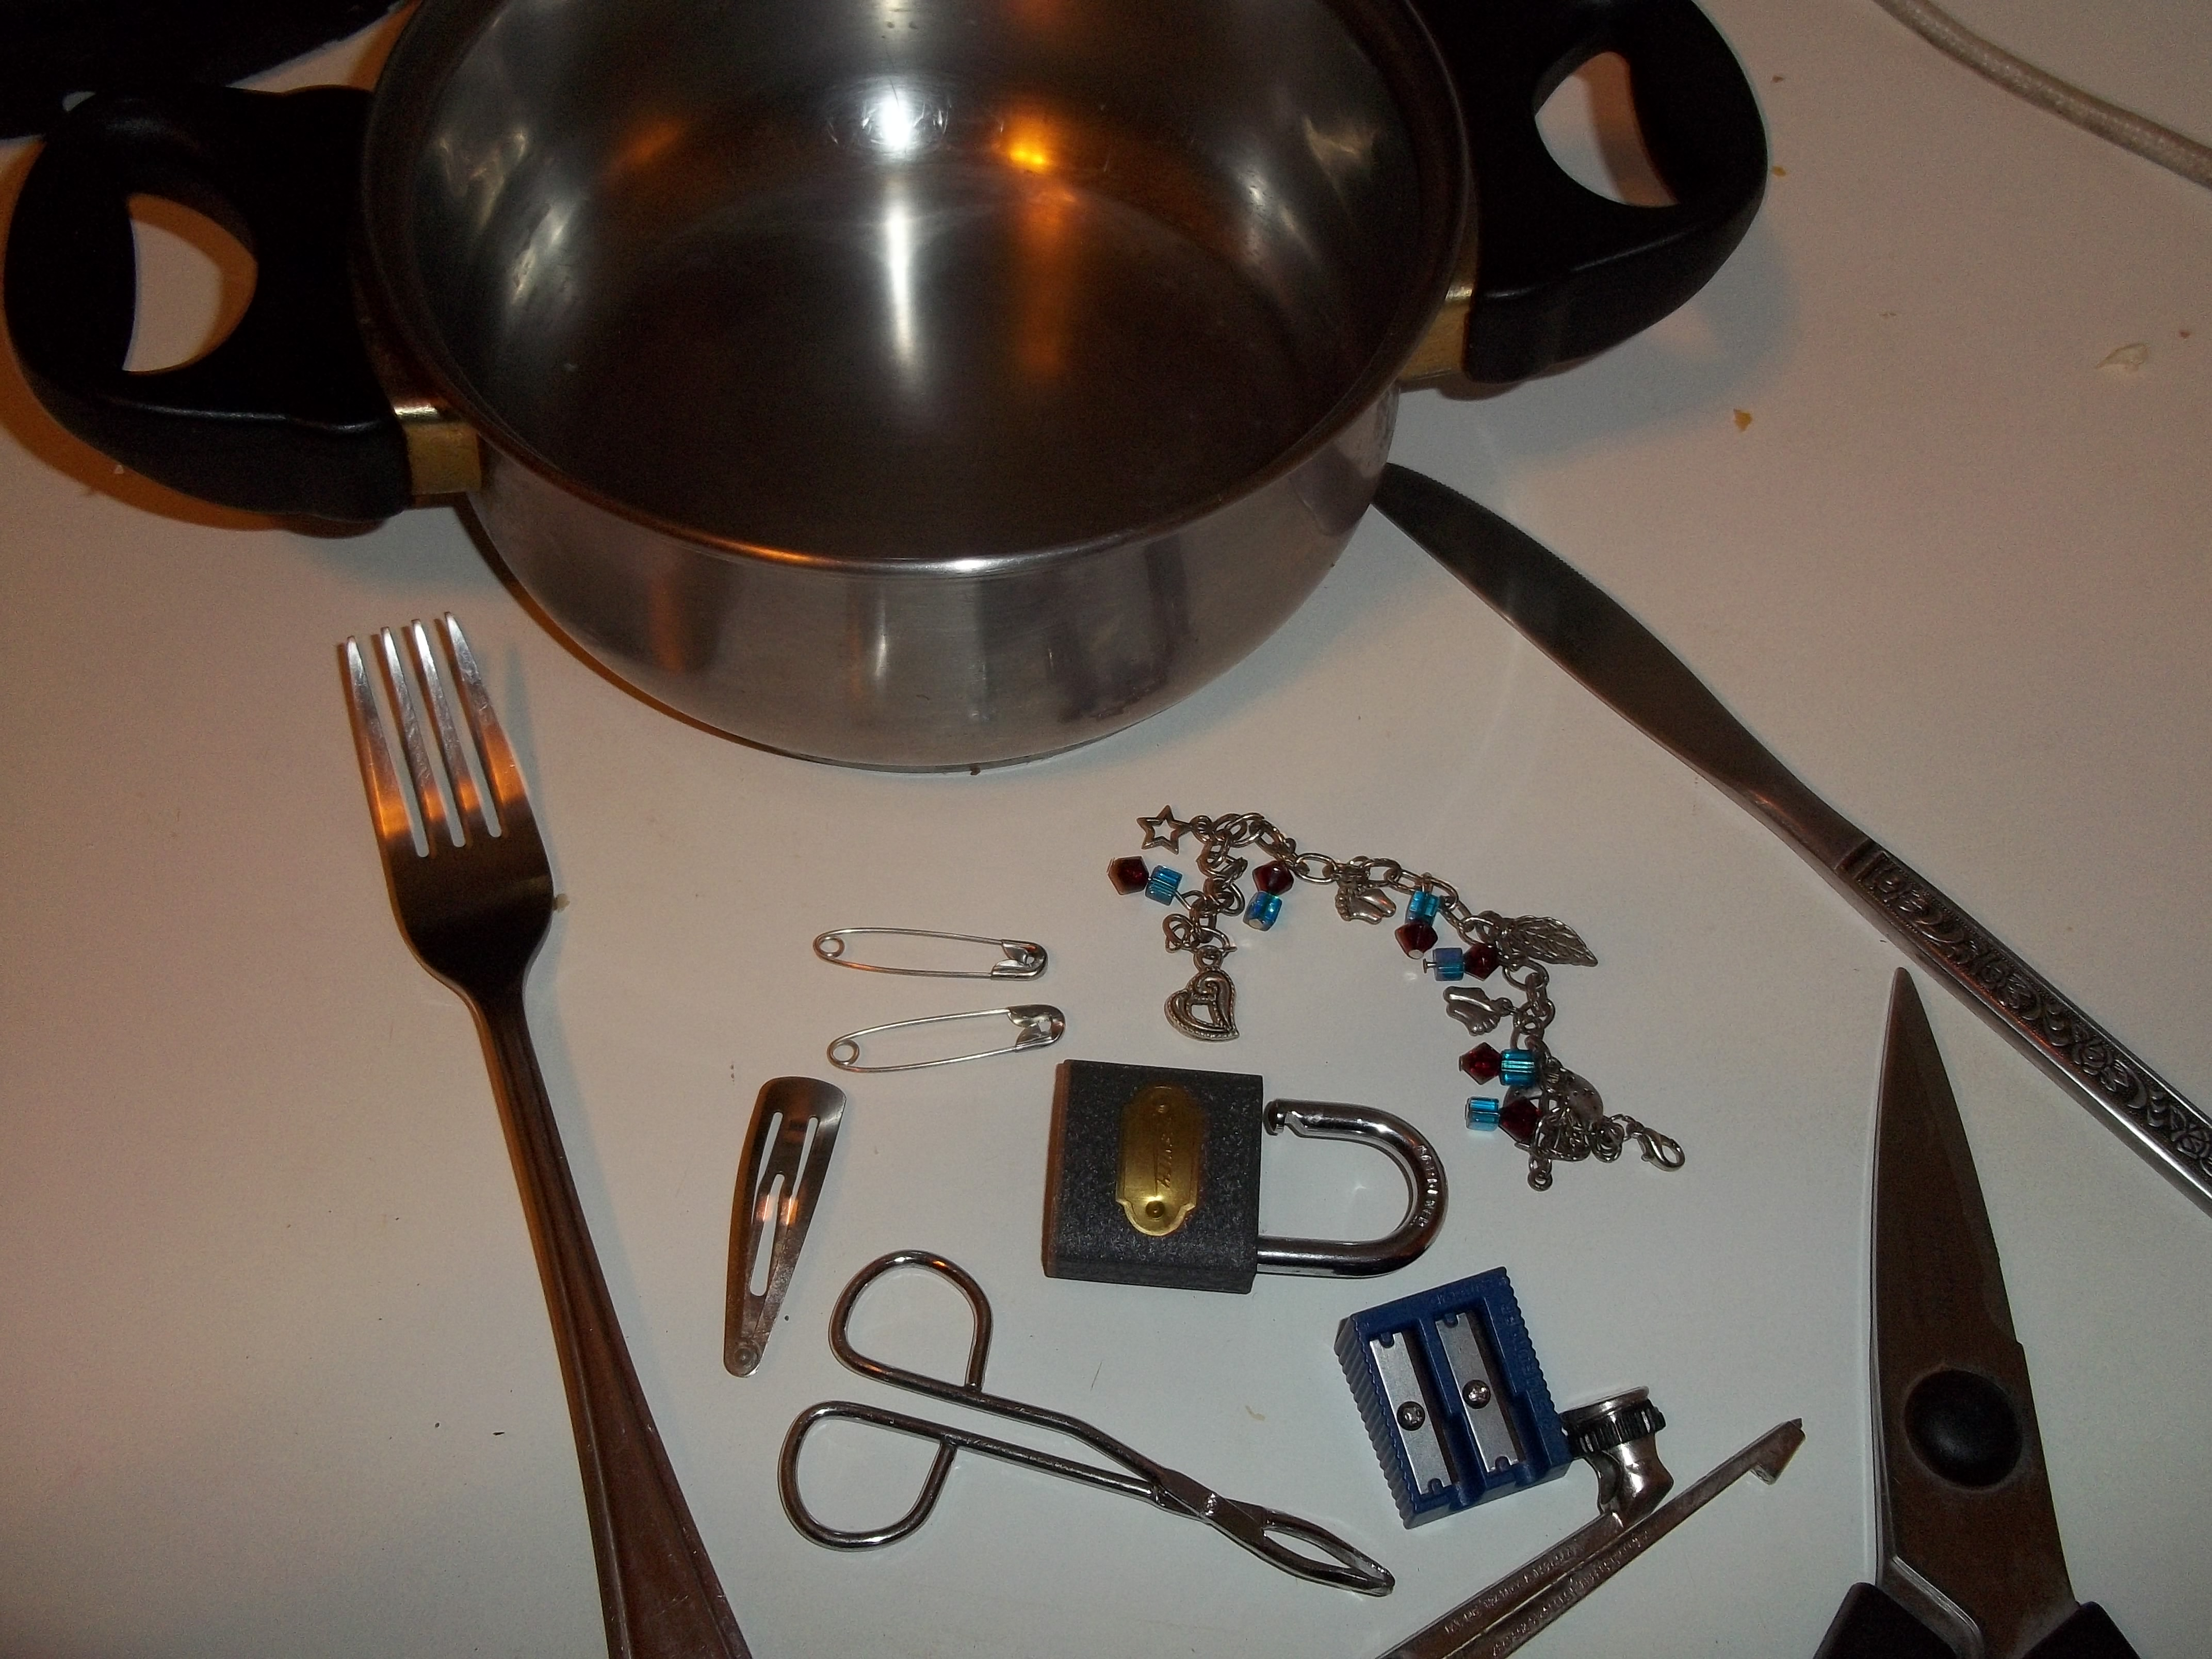
\includegraphics[width=.8\textwidth]{photos/metal_objects.jpg}\par
\end{center}
\end{minipage}
}
\end{activity}
      \label{m38708*uid93}
            \subsection*{Nie-metale}
            \nopagebreak
\begin{minipage}{.5\textwidth}
        \label{m38708*id66021}In teenstelling met metale, is nie-metale swak termiese geleiers, goeie elektriese isoleerders (wat beteken dat hulle \textsl{nie} elektrisiteit gelei nie) en nie pletbaar of smeebaar nie. Die nie-metale sluit elemente soos swawel ($\text{S}$), fosfor ($\text{P}$), stikstof ($\text{N}$) en suurstof ($\text{O}$) in.\par 
\end{minipage}
\begin{minipage}{.5\textwidth}
\begin{center}
 \includegraphics[width=.4\textwidth]{photos/sulphurby-nickstone333.jpg}\par
\textit{Prent verskaf deur nickstone333 op Flickr.com}
\end{center}
\end{minipage}
      \label{m38708*uid94}
            \subsection*{Metallo\"ide}
            \nopagebreak
\begin{minipage}{.5\textwidth}
        \label{m38708*id66042}Metallo\"ide of semi-metale, het meestal nie-metaaleienskappe. Een van hulle onderskeidende eienskappe is dat hulle geleidingsvermoë toeneem as hul temperatuur verhoog. Dit is die teenoorgestelde van wat gebeur in metale.  Di\'e eienskap is bekend as halfgeleiding en die stof word  'n halfgeleier genoem. Halfgeleiers is belangrik in elektronika, soos rekenaars en selfone. Die metallo\"ide sluit elemente soos silikon ($\text{Si}$) en germanium ($\text{Ge}$) in.\par 
\end{minipage}
\begin{minipage}{.5\textwidth}
\begin{center}
 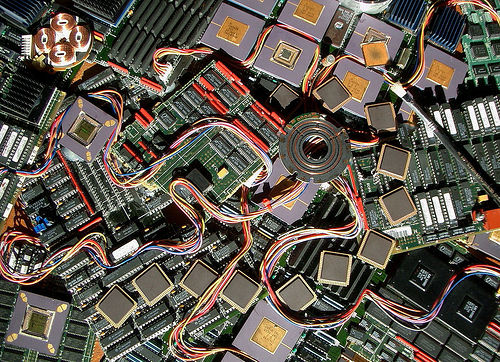
\includegraphics[width=.6\textwidth]{photos/siliconby-jurveston.jpg}\par
\textit{Prent verskaf deur jurveston op Flickr.com}
\end{center}
\end{minipage}
\par 
      \noindent
   %   \hspace*{-30pt}
\includegraphics[width=0.5in]{col11305.imgs/pspencil2.png}   \raisebox{25mm}{   
   %   \begin{mdframed}[linewidth=4, leftmargin=40, rightmargin=40]  
%       \begin{wex}{Metals, metalloids and non-metals 1}{\label{m38708*eip-77}
%   \label{m38708*eip-252}
% For each of the following substances state whether they are metals, metalloids or non-metals, using their position on the periodic table.
% \label{m38708*eip-id1170734629720}
% \begin{enumerate}[noitemsep, label=\textbf{\alph*}. ] 
%             \leftskip=20pt\rightskip=\leftskip
% \item Oxygen
% \item Arsenic
% \item Vanadium
% \item Potassium
% \end{enumerate}
%   \par }
% {\vspace{5pt}
% %\label{m38708*eip-149}\noindent\textbf{Solution to Exercise }
% %\label{m38708*eip-id1170750216596}\begin{enumerate}[noitemsep, label=\textbf{\alph*}. ] 
% %            \leftskip=20pt\rightskip=\leftskip
% \westep {Look at the periodic table} 
% \begin{enumerate}[noitemsep, label=\textbf{\alph*}. ]
% \item Oxygen is on the right of the zigzag line and so is a non-metal.
% \item Arsenic is on the zigzag line and is a metalloid.
% \item Vanadium is on the left of zigzag line and so is a metal.
% \item Potassium is on the left of the zigzag line and so is a metal.\end{enumerate}
% }
%     \end{wex}
%  %   \end{mdframed}
%   %  }
% %    \noindent
%   \par
% %            \label{m38708*eip-173}\vspace{.5cm} 
% %      \noindent
% %      \hspace*{-30pt}
\includegraphics[width=0.5in]{col11305.imgs/pspencil2.png}   \raisebox{25mm}{   
% %      \begin{mdframed}[linewidth=4, leftmargin=40, rightmargin=40]  
%       \begin{wex}{Metals, metalloids and non-metals 2}{\label{m38708*eip-757}
%   \label{m38708*eip-25442}For each of the following substances state whether they are metals, metalloids or non-metals, using the information given.
% \label{m38708*eip-id1170742635239}
% \begin{enumerate}[noitemsep, label=\textbf{\alph*}. ] 
%             \leftskip=20pt\rightskip=\leftskip
% \item Aluminium in a cooking pot
% \item Silicon in a computer chip
% \item Plastic insulation around a wire
% \item Silver jewellery\end{enumerate}
%   \par }
% {\vspace{5pt}
% %\label{m38708*eip-1455}\noindent\textbf{Solution to Exercise }
% %\label{m38708*eip-id1170755988427}\begin{enumerate}[noitemsep, label=\textbf{\alph*}. ] 
%  %           \leftskip=20pt\rightskip=\leftskip
% \westep{Use what you know} \begin{enumerate}[noitemsep, label=\textbf{\alph*}. ]
% \item A cooking pot needs to be able to conduct heat and so the aluminium used must be a metal.
% \item Computer chips rely on semi-conductors and all metalloids are semiconductors. So silicon is a metalloid.
% \item The plastic around the wire must be insulating to current and so is a non-metal.
% \item Silver in the jewellery is chosen for its malleability and shiny lustre. So silver is a metal.
% \end{enumerate}}
%     \end{wex}
%    \end{mdframed}
%    }
    \noindent
%   \label{m38708**end}
%          \section{Properties}
%     \nopagebreak



\section{Elektriese geleiers, halfgeleiers en isoleerders}
\nopagebreak

\label{m38706*id66058} 

\Definition{Elektriese geleier}{'n Elektriese geleier is 'n stof wat dit moontlik maak vir 'n elektriese stroom om daardeur te vloei.} Elektriese geleiers is gewoonlik metale. \textsl{Koper} is een van die beste elektriese geleiers, en
dit is waarom dit gebruik word om geleidingsdraad te maak. In werklikheid, het \textsl{silwer} eintlik 'n nog hoër elektriese geleidingsvermoë as koper, maar silwer is te duur om te gebruik.\par \\

\mindsetvid{conductors and insulators}{VPaex} 

\begin{minipage}{0.5\textwidth}In die oorhoofse kraglyne wat ons sien hierbo
is \textsl{aluminium} gebruik. Die aluminium omsluit  'n staalkern wat dit versterk sodat dit nie breek wanneer dit oor lang afstande gerek word nie. Somtyds word goud as draad gebruik want dit is baie bestand teen oppervlakkorrosie (roes). \textsl{Korrosie} is wanneer 'n stof begin om te verswak as gevolg van sy reaksies met suurstof en water in die lug.\par 
\end{minipage}
\begin{minipage}{.5\textwidth}
\begin{center}
 \includegraphics[height=.4\textwidth]{photos/Tripp.jpg}\par
\textit{Prent verskaf deur Tripp op Flickr.com}
\end{center}
\end{minipage}
%       \label{m38706*id66098} 'n \textbf{Isoleerder} is 'n nie-geleidende stof wat nie 'n elektriese lading kan gelei nie.  
% \Definition
% %	  \begin{tabular*}{15 cm}{m{15 mm}m{}}
% %	\hspace*{-50pt}  
\includegraphics[width=0.5in]{col11305.imgs/psflag2.png}   & \Definition{   \label{id2409398}\textbf{ 
% {Geleiers} 
% %}} { \label{m38706*meaningfhsst!!!underscore!!!id354}
% %      \label{m38706*id66124}
% { 'n Geleier laat die maklike beweging of vloei van iets soos warmte of elektriese lading deur.\par 
%        } 
\Definition{Isoleerder}
{Isoleerders is die teenoorgestelde van geleiers omdat hulle die vloei van warmte of elektriese lading deur hulle inhibeer (stuit) of verminder.\par}
Plastiek en hout is voorbeelde van isoleerders. \textbf{Halfgeleiers} tree op soos isoleerders wanneer hulle koud is, en soos geleiers wanneer hulle warm is. Die elemente silikon en germanium is voorbeelde van halfgeleiers.\par
%      \end{tabular*}
%      \end{definition}
\label{m38706*secfhsst!!!underscore!!!id357}
            \begin{g_experiment}{Elektriese geleidingsvermo\"e}{
            \nopagebreak
            \label{m38706*id66151}\noindent{}\textbf{Doel:}
        \newline
     Om die elektriese geleidingsvermoë van 'n aantal stowwe te ondersoek.\par 
      \label{m38706*id66166}\noindent{}\textbf{Apparaat:} \\
\begin{minipage}{.5\textwidth}
      \label{m38706*id66175}\begin{itemize}[noitemsep]
            \label{m38706*uid95}\item twee of drie selle
\label{m38706*uid96}\item gloeilamp
\label{m38706*uid97}\item krokodilklampe
\label{m38706*uid98}\item geleidingsdrade
\label{m38706*uid99}\item 'n versameling stowwe om te toets (bv. 'n stuk plastiek, aluminium houer, metaal potloodskerpmaker, magneet, hout, kryt, lap).
\end{itemize}
\end{minipage}
\begin{minipage}{.5\textwidth}
      \label{m38706*id66241}
    \setcounter{subfigure}{0}
	\begin{figure}[H] % horizontal\label{m38706*id66244}
    \begin{center}
\scalebox{0.7}{
\begin{pspicture}(0,-0.6)(5,6)
\SpecialCoor
%\psgrid[gridcolor=lightgray]
\pnode(0,0){A}
\pnode(0,5){B}
\pnode(5,5){C}
\pnode(5,0){D}
\pnode(3.5,0){E}
\pnode(1.5,0){F}
\rput{90}{\lamp(A)(B){gloeilamp}}
\battery(B)(C){selle}
\psline(C)(D)
\psline[arrowsize=10pt,arrowinset=0,arrowlength=2.5]{->}(D)(E)
\psframe(1.5,-0.5)(3.5,0.5)
\uput[u](2.5,0.5){toetsstof}
\rput(2.5,0){X}
\psline(4,0)(4,-0.4)(4.6,-0.4)
\uput[r](4.6,-0.4){krokodilklampe}
\psline[arrowsize=10pt,arrowinset=0,arrowlength=2.5]{<-}(F)(A)
\end{pspicture}
}
    \end{center}
 \end{figure}  
\end{minipage}     
      \par 
\label{m38706*id66251}\noindent{}\textbf{Metode:}
\newline
\begin{enumerate}[noitemsep, label=\textbf{\arabic*}. ] 
\item Verbind die stroombaan soos hierbo getoon, sodat die toetsstof tussen die twee krokodil\-klampe gehou word. Die geleidingsdrade moet aan die selle verbind word en die gloei\-lamp moet ook in die stroombaan gekoppel word.

\item Plaas die toets stowwe een vir een tussen die krokodilklampe en kyk wat gebeur met die gloeilamp. As die gloeilamp brand beteken dit die stroomvloei en die stof wat jy toets is 'n \textbf{elektriese geleier}.
\end{enumerate}
        \par 
      \label{m38706*id66291}\noindent{}\textbf{Resultate:}
        \newline
        Teken jou resultate in die tabel hieronder op:
    % \textbf{m38706*id66304}\par
          \begin{table}[H]
    % \begin{table}[H]
    % \\ '' '0'
        \begin{center}
      \label{m38706*id66304}
    \noindent
      \begin{tabular}{|p{2cm}|p{2cm}|p{2cm}|p{2cm}|}\hline
                \textbf{Toetsstof}
               &
                \textbf{Metaal/nie-metaal}
               &
                \textbf{Brand die gloeilamp?}
               &
                \textbf{Geleier of isoleerder}
            \\ \hline
         &
         &
         &
       \\ \hline
         &
         &
         &
       \\ \hline
         &
         &
         &
        \\ \hline
         &
         &
         &
        \\ \hline
    \end{tabular}
      \end{center}
\end{table}
    \par
  \par 
      \label{m38706*id66494}\noindent{}\textbf{Gevolgtrekkings:}
        \newline
        In die stowwe wat getoets is, was die metale in staat om elektrisiteit te gelei, die nie-metale kon nie. Metale is goeie geleiers van elektrisiteit en nie-metale is swak geleiers van elektrisiteit. }
            \end{g_experiment}
\simulation{}{VPcyz}
% \label{m38706*eip-316}The following simulation allows you to work through the above activity. For this simulation use the grab bag option to get materials to test. Set up the circuit as described in the activity.
%     \setcounter{subfigure}{0}
% 	\begin{figure}[H] % horizontal\label{m38806*transverse-waves}
%     \textnormal{PhET simulation for electrical conductivity}\nopagebreak
%   \label{m38806*phet!!!underscore!!!sim}\label{m38806*phet-simulation}
%             \raisebox{-5 pt}{ 
\includegraphics[width=0.5cm]{col11305.imgs/summary_www.png}} { (Simulation:  lbK )}
%  \end{figure}    
%         \par 
    \label{m38706*cid7}
            \section{Termiese Geleiers en Isoleerders}
            \nopagebreak
      \label{m38706*id66527} 'n \textbf{Termiese geleier} is 'n stof (materiaal) wat toelaat dat energie, in die vorm van hitte, oorgedra word binne die stof sonder enige beweging van die stof self. 'n Maklike manier om hierdie begrip te verstaan is deur middel van 'n eenvoudige demonstrasie.\par 

\mindsetvid{which material is the better insulator}{VPafb} 

\label{m38706*secfhsst!!!underscore!!!id453}
            \begin{g_experiment}{Demonstrasie: Termiese geleidingsvermo\"e}{
            \nopagebreak
            \label{m38706*id66568}\noindent{}\textbf{Doel: }\newline
      Om verskillende stowwe se vermoë van hitte te gelei, te demonstreer.\par 
      \label{m38706*id66588}\noindent{}\textbf{Apparaat: }\newline
\begin{minipage}{.5\textwidth}
Jy benodig:
\begin{itemize}
 \item twee koppies (gemaak van dieselfde materiaal bv. plastiek)
\item 'n metaallepel
\item 'n plastiese lepel.
\end{itemize} 
\end{minipage}
\begin{minipage}{.5\textwidth}
	\begin{figure}[H] % horizontal\label{m38706*id66244}
    \begin{center}
\scalebox{0.5}{
\begin{pspicture}(-5,-5)(5,5)
\psset{unit=1cm}
\newpsstyle{white} {linestyle=solid,linewidth=.1,fillstyle=none}
\uput[r](-3,1){\Large{kookwater}}
\psline[linewidth=0.04]{->}(-0.3,1)(0.5,1)
\uput[r](-3,3){\Large{plastieklepel}}
\psline[linewidth=0.04]{->}(-0.25,3)(0.2,3)
\psline[linewidth=0.1](1.95,0)(0.25,3.2)
\pstTubeEssais[glassType=becher,aspectLiquide1=white]
\uput[r](3.5,1){\Large{kookwater}}
\psline[linewidth=0.04]{->}(3.55,1)(2.6,1)
\uput[r](3.5,3){\Large{metaallepel}}
\psline[linewidth=0.04]{->}(3.55,3)(3,3)
\psline[linewidth=0.1](0.95,0)(3,3.2)
\pstTubeEssais[glassType=becher,aspectLiquide1=white]
\end{pspicture}}
    \end{center}
 \end{figure} 
\end{minipage}
      \label{m38706*id66592}\textbf{Metode:}
\label{m38706*id66609}\begin{itemize}[noitemsep]
\label{m38706*uid102}\item Gooi die twee koppies omtrent halfvol kookwater.
\label{m38706*uid103}\item Plaas 'n metaallepel in een van die koppies en 'n plastiese lepel in die ander een en hou die lepels vas aan die teenoorgestelde punte.
\label{m38706*uid104}\item Let op watter lepel die vinnigste warm word.
\end{itemize}
        \par 
\label{m38706*eip-270}
%\begin{tabular}{cc}
%	\hspace*{-50pt}\raisebox{-8 mm}{\hspace{-0.2in}
\includegraphics[width=0.5in]{col11305.imgs/pstip2.png} } & 
%	\begin{minipage}{0.85\textwidth}
%	\begin{note}
      \Warning{Wees versigtig wanneer jy met kookwater werk en wanneer jy aan die lepels raak, jy kan jouself maklik brand.}
%	\end{note}
%	\end{minipage}
%	\end{tabular}
	\par
      \label{m38706*id66666}\noindent{}\textbf{Resultate: }\newline
     Die metaallepel verhit vinniger as die plastieklepel. Met ander woorde, die metaal gelei hitte goed, maar die plastiek nie.\par 
\label{m38706*id66687}\noindent{}\textbf{Gevolgtrekking: }Metaal is 'n goeie termiese geleier, terwyl die plastiek 'n swak termiese geleier is.}
\end{g_experiment}
 \par 


\IFact{Goed ge\"isoleerde geboue benodig min\-der en\-er\-gie vir ver\-warm\-ing as geboue wat geen isolering het nie.
Twee boumateriale wat alhoemeer w\^ereldwyd gebruik word, is \textbf{mineraalwol} en \textbf{polistireen}. Mineraalwol is 'n goeie isoleerder, want dit hou die lug nogsteeds in die matriks (binne) van die wol sodat hitte nie verlore gaan nie. Aangesien lug 'n swak geleier en 'n goeie isoleerder is, help dit om energie binne die gebou te hou. Polistireen is ook 'n goeie isoleerder en is dartoe in staat om koel goed koel te hou en warm goed warm te hou. Dit het die bykomende voordeel dat dit weerstand bied teen vog, muf en skimmel.}
      \label{m38706*id66699} 'n \textbf{Isoleerder} is 'n stof (materiaal) wat nie die oordrag van elektrisiteit of warmte energie toelaat nie. Stowwe wat swak hitte geleiers is, kan ook beskryf word as goeie hitte (termiese) isoleerders.\par 


% \label{m38706*notfhsst!!!underscore!!!id490}
% \begin{tabular}{cc}
% 	\hspace*{-50pt}\raisebox{-8 mm}{\hspace{-0.2in}
\includegraphics[width=0.75in]{col11305.imgs/psfact2.png} } & 
% 	\begin{minipage}{0.85\textwidth}
% 	\begin{note}
%       {note: }Water is a better thermal conductor than air and conducts heat away from the body about 20 times more efficiently than air. A person who is not wearing a wetsuit, will lose heat very quickly to the water around them and can be vulnerable to hypothermia (this is when the body temperature drops very low). Wetsuits help to preserve body heat by trapping a layer of water against the skin. This water is then warmed by body heat and acts as an insulator. Wetsuits are made out of closed-cell, foam neoprene. Neoprene is a synthetic rubber that contains small bubbles of nitrogen gas when made for use as wetsuit material. Nitrogen gas has very low thermal conductivity, so it does not allow heat from the body (or the water trapped between the body and the wetsuit) to be lost to the water outside of the wetsuit. In this way a person in a wetsuit is able to keep their body temperature much higher than they would otherwise.
% 	\end{note}
% 	\end{minipage}
% 	\end{tabular}
	\par
\label{m38706*secfhsst!!!underscore!!!id492}
            \begin{Investigation}{ 'n Nadere kykie na termiese geleidingsvermo\"e}
{            \nopagebreak
      \label{m38706*id66744}      Kyk na die tabel hieronder, dit toon die termiese geleidingsvermo\"e van 'n aantal verskillende materiale en beantwoord dan die vrae wat volg. Hoe ho\"er die getal in die tweede kolom, hoe beter sal die materiaal hitte gelei (d.w.s. dit is 'n goeie termiese geleier). Onthou dat 'n materiaal wat hitte doeltreffend gelei, ook hitte vinniger sal verloor as 'n isolerende materiaal.\par 
    % \textbf{m38706*id66753}\par
          \begin{table}[H]
    % \begin{table}[H]
    % \\ '' '0'
        \begin{center}
      \label{m38706*id66753}
    \noindent
      \begin{tabular}{|l|l|}\hline
\textbf{Materiaal} & \textbf{Termiese geleidingsvermoë} \\ 
                 &  \textbf{($\text{W}\ensuremath{\cdot}\text{m}{}^{-1}\ensuremath{\cdot}\text{K}{}^{-1}$) } \\ \hline
Silwer & 429 \\ \hline
Vlekvrye staal & 16 \\ \hline
Standaard glas & 1.05 \\ \hline
Beton & 0.9 - 2 \\ \hline
Rooi baksteen & 0.69 \\ \hline
Water & 0.58 \\ \hline
Poli\"etileen (plastiek) & 0.42 - 0.51 \\ \hline
Hout & 0.04 - 0.12 \\ \hline
Polistireen & 0.03 \\ \hline
Lug & 0.024 \\ \hline
    \end{tabular}
      \end{center}
%    \begin{center}{\small\bfseries Table 1.4}\end{center}
%    \begin{caption}{\small\bfseries Table 1.4}\end{caption}
\end{table}
    \par
      \label{m38706*id67009}Gebruik hierdie inligting om die volgende vrae te beantwoord:\par 
      \label{m38706*id67013}\begin{enumerate}[noitemsep, label=\textbf{\arabic*}. ] 
            \label{m38706*uid105}\item Noem twee materiale wat goeie termiese geleiers is.
\label{m38706*uid106}\item Noem twee materiale wat goeie isoleerders is.
\label{m38706*uid107}\item Verduidelik waarom:
\label{m38706*id67053}\begin{enumerate}[noitemsep, label=\textbf{\alph*}. ] 
            \label{m38706*uid108}\item Rooi baksteen 'n beter keuse is as beton vir die bou van huise wat minder interne verwarming benodig.
\label{m38706*uid109}\item Vlekvrye staal goed is vir die maak van kookpotte.
\end{enumerate}
        \end{enumerate}}
\end{Investigation}
\label{m38706*notfhsst!!!underscore!!!id564}
%\begin{tabular}{cc}
%	\hspace*{-50pt}\raisebox{-8 mm}{\hspace{-0.2in}
\includegraphics[width=0.75in]{col11305.imgs/psfact2.png} } & 
%	\begin{minipage}{0.85\textwidth}
%	\begin{note}
%	\end{note}
%	\end{minipage}
%	\end{tabular}
	\par
    \label{m38706*cid8}
            \section{Magnetiese en nie-magnetiese materiale}
            \nopagebreak
      \label{m38706*id67151}Ons het nou gekyk na 'n aantal maniere waarop materie gegroepeer kan word, soos in metale, semi-metale en nie-metale, elektriese geleiers en isoleerders, en termiese geleiers en isoleerders. 'n Manier waarop ons metale verder kan groepeer, is om hulle te verdeel in di\'e wat \textbf{magneties} is en di\'e wat \texbf{nie-magneties} is.\par 
\mindsetvid{magnetic materials}{VPaga} 
%             \label{m38706*fhsst!!!underscore!!!id570}\begin{definition}
% 	  \begin{tabular*}{15 cm}{m{15 mm}m{}}
% 	\hspace*{-50pt}  
\includegraphics[width=0.5in]{col11305.imgs/psflag2.png}   & 
\Definition{   \label{id2410309} { Magnetisme }} { \label{m38706*meaningfhsst!!!underscore!!!id570}
      \label{m38706*id67174}       Magnetisme is 'n krag wat sekere soorte voorwerpe, genoem ``magnetiese'' voorwerpe, op mekaar kan uitoefen sonder om fisies te raak. 'n Magnetiese voorwerp is omring deur 'n magnetiese veld wat swakker word as 'n mens verder weg van die voorwerp beweeg.\par 
       } 
\begin{minipage}{.5\textwidth}
      \label{m38706*id67186} 'n Metaal word as \texbf{ferromagneties} beskou as dit gemagnetiseer kan word (d.w.s. mens kan daarvan 'n magneet maak). As jy 'n magneet baie naby aan 'n metaal voorwerp hou, kan dit gebeur dat 'n magneetveld gewek word in die metaal voorwerp en die metaal voorwerp dus magneties word. Sommige metale behou hulle magnetisme langer as ander. Ons kyk na yster en staal as voorbeeld. Yster verloor sy magnetisme redelik vinnig as dit weg van die magneet af geneem word. Staal sal vir 'n lang tyd magneties bly. Staal word dikwels gebruik vir die maak van permanente magnete wat vir 'n verskeidenheid doeleindes gebruik word.\par 
\end{minipage}
\begin{minipage}{.5\textwidth}
\begin{center}
 \includegraphics[width=.8\textwidth]{photos/magnet.jpg}\par
\textit{Prent verskaf deur Aney op Wikimedia}
\end{center}
\end{minipage}\par
      \label{m38706*id67200}Magnete word gebruik om metale in 'n skrootwerf te sorteer, in kompasse om rigting te vind, in magnetiese stroke van video-bande en OTM-kaarte waar inligting gestoor moet word, in rekenaars en TV's, asook in kragopwekkers en elektriese motors.
\par 
\label{m38706*secfhsst!!!underscore!!!id575}
            \begin{Investigation}{Magnetisme}{
            \nopagebreak
      \label{m38706*id67220}      Jy kan toets of 'n voorwerp magneties is of nie deur 'n magneet naby dit te hou. As die voorwerp deur die magneet aangetrek word, is dit magneties.\par 
      \label{m38706*id67227}Vind vyf voorwerpe in die klaskamer of by jou huis en toets of hulle magneties is of nie. Voltooi dan die onderstaande tabel:\par 
    % \textbf{m38706*id67234}\par
          \begin{table}[H]
    % \begin{table}[H]
    % \\ '' '0'
        \begin{center}
      \label{m38706*id67234}
    \noindent
      \begin{tabular}{|p{3cm}|p{1.5cm}|}\hline
                \textbf{Voorwerp}
               &
                \textbf{Magneties of nie-magneties} \\ \hline
         & \\ \hline
         & \\ \hline
         & \\ \hline
         & \\ \hline
         & \\ \hline
    \end{tabular}
      \end{center}
%     \begin{center}{\small\bfseries Table 1.5}\end{center}
%     \begin{caption}{\small\bfseries Table 1.5}\end{caption}
\end{table}}

\end{Investigation}
    \par
\label{m38706*secfhsst!!!underscore!!!id616}
            \begin{groupdiscussion}{Eienskappe van materiale}{
            \nopagebreak
      \label{m38706*id67392} In groepe van 4-5, bespreek hoe kennis van die eienskappe van stowwe dit moontlik gemaak het dat:\par 
\begin{itemize}[noitemsep]
    \item die gemeenskap gevorderde rekenaartegnologie kan ontwikkel
    \item huise van elektrisiteit voorsien word
    \item die samelewing maniere kan vind om energie te bespaar
\end{itemize}
\end{groupdiscussion}
% \label{m38706*eip-968}Die volgende voorstelling verskaf 'n opsomming van die klassifikasie van materie.
%     \setcounter{subfigure}{0}
% 	\begin{figure}[H] % horizontal\label{m38706*slidesharefigure}
%     \label{m38706*slidesharemedia}\label{m38706*slideshareflash}\raisebox{-5 pt}{ 
\includegraphics[width=0.5cm]{col11305.imgs/summary_www.png}} { (Voorstelling:  P10013 )}
%       \vspace{2pt}
%     \vspace{.1in}
%  \end{figure}       \par
}
\end{discussion} \label{m38706*cid9}


\summary{VPcyl}
\nopagebreak
\begin{itemize}[noitemsep]
     \item Al die voorwerpe en stowwe wat ons in die wêreld sien word gemaak van \textbf{materie}.
     \item Hierdie materie kan geklassifiseer word as \textbf{mengsels} en \textbf{suiwer stowwe}.
     \item 'n \textbf{Mengsel} is 'n kombinasie (samevoeging) van een of meer stowwe wat nie chemies met mekaar verbind nie mekaar. Voorbeelde van mengsels is lug ( 'n mengsel van verskillende gasse) en ontbytgraan in melk.
     \item Die belangrikste \texbf{kenmerke} van mengsels is dat die stowwe waaruit die mengsel bestaan nie 'n vaste verhouding het nie, hulle behou hulle individuele eienskappe en hulle kan van mekaar op 'n meganiese manier geskei word.
     \item 'n \texbf{Heterogene mengsel} is nie-uniform (nie-eenvormig) – d.w.s. die verskillende dele van die mengsel kan gesien word. 'n Mengsel van sand en water dien as voorbeeld.
     \item 'n \texbf{Homogene mengsel} is uniform, die verskillende komponente van die mengsel kan nie gesien word nie. Sout in water dien as voorbeeld.
     \item Suiwer stowwe kan verder verdeel word in \textbf{elemente} en \textbf{verbindings}.
     \item 'n \textbf{Element} is 'n stof wat nie opgebreek kan word in eenvoudiger stowwe deur chemiese metodes nie.
     \item Al die elemente is in die \textbf{Periodieke Tabel} aangeteken. Elke element het sy eie chemiese simbool. Voorbeelde hiervan is yster ($\text{Fe}$), swawel ($\text{S}$), kalsium ($\text{Ca}$), magnesium ($\text{Mg}$) en fluoor ($\text{F}$).
     \item 'n \textbf{Verbinding} is 'n stof wat bestaan uit twee of meer elemente wat chemies
in 'n vaste verhouding aan mekaar verbind is. Voorbeelde van verbindings is natriumchloried ($\text{NaCl}$),
ystersulfied ($\text{FeS}$), kalsiumkarbonaat (${\text{CaCO}}_{3}$) en water (${\text{H}}_{2}\text{O}$).
     \item Tydens die \textbf{benoeming van verbindings} en die skryf van \textbf{chemiese formules} is dit belangrik om  te weet watter elemente in die verbinding voorkom, hoeveel atome van elk van hierdie elemente sal verbind en waar die elemente in die Periodieke Tabel voorkom. 'n Aantal re\"els kan dan gevolg word om die verbinding te benoem.
     \item Materie kan op nog 'n manier geklassifiseer word, naamlik: \textbf{metale} (soos yster, goud, koper), \textbf{metallo\"ide} (bv. silikon en germanium) en \textbf{nie-metale} (soos swawel, fosfor en stikstof).
     \item \textbf{Metale} is goeie elektriese en termiese geleiers, het 'n blink glans, is pletbaar en smeebaar en het 'n ho\"e smeltpunt. Hierdie eienskappe maak metale baie nuttig vir gebruik as elektriese drade, in kookgerei, vir juwele en baie ander toepassings.
     \item 'n Verdere manier van klassifikasie van materie is in \textbf{elektriese geleiers}, \textbf{halfgeleiers} en \textbf{isoleerders}.
     \item 'n \textbf{Elektriese geleier} laat toe dat 'n elektriese stroom daardeur vloei. Die meeste metale is goeie elektriese geleiers.
     \item 'n \textbf{Elektriese isoleerder} laat nie die deurgang van 'n elektriese stroom toe nie. Voorbeelde hiervan is plastiek, hout, katoenmateriaal en keramiek.
     \item Stowwe (materiale) kan ook geklassifiseer word as \textbf{termiese geleiers} of \textbf{termiese isoleerders} afhangende daarvan of hulle in staat is om hitte te gelei of nie.
     \item Stowwe kan ook \textbf{magneties} of \textbf{nie-magneties} wees.
\end{itemize} \pagebreak

\label{m38706*secfhsst!!!underscore!!!id672}

\begin{eocexercises}{Klassifikasie van Materie}{
\nopagebreak
\begin{enumerate}[noitemsep, label=\textbf{\arabic*}. ] 
        \item Watter van die volgende kan geklassifiseer word as 'n mengsel:
        \begin{enumerate}[noitemsep, label=\textbf{\alph*}. ] 
            \item suiker
            \item tafelsout
            \item lug
            \item yster
        \end{enumerate}
        \item 'n Element kan gedefinieer word as:
        \begin{enumerate}[noitemsep, label=\textbf{\alph*}.] 
            \item 'n Stof wat nie in twee of meer stowwe geskei kan word deur gewone chemiese (of fisiese) metodes nie.
            \item 'n Stof met 'n konstante samestelling.
            \item 'n Stof wat bestaan uit twee of meer stowwe, in 'n definitiewe massaverhouding.
            \item 'n Eenvormige stof.
        \end{enumerate}

    \item Klassifiseer elk van die volgende stowwe as 'n \textsl{element}, 'n \textsl{verbinding}, 'n \textsl{homogene mengsel}, of 'n \textsl{heterogene mengsel}: sout, suiwer water, grond, soutwater, suiwer lug, koolstofdioksied, goud en brons.\newline
    \item Kyk na die tabel hieronder. In die eerste kolom (A) is 'n lys van stowwe. In die tweede kolom (B) is 'n beskrywing van die groep waaraan elk van hierdie stowwe behoort. Pas die \textsl{stof} in Kolom A by die \textsl{beskrywing} in Kolom B.
% \textbf{m38706*id68147}\par
\begin{table}[H]
% \begin{table}[H]
% \\ 'id2880342' '1'
\begin{center}
\label{m38706*id68147}
\begin{tabular}{|l|l|}\hline
\textbf{Kolom A} & \textbf{Kolom B} \\ \hline
\textbf{1.} yster & \textbf{A.} 'n verbinding met 2 elemente \\ \hline
\textbf{2.} H$_\text{2}$S & \textbf{B.} 'n heterogene mengsel \\ \hline
\textbf{3.} suikeroplossing & \textbf{C.} 'n metaalallooi \\ \hline
\textbf{4.} sand en klippe & \textbf{D.} 'n element \\ \hline
\textbf{5.} staal & \textbf{E.} 'n homogene mengsel \\ \hline
\end{tabular}
\end{center}
%     \begin{center}{\small\bfseries Table 1.6}\end{center}
%     \begin{caption}{\small\bfseries Table 1.6}\end{caption}
\end{table}
\par
\item 'n Proefbuis wat 'n mengsel van ystervylsels en swawel bevat is aan jou gegee. Jy word gevra om die hoeveelheid yster in die monster te weeg. 
\begin{enumerate}[noitemsep, label=\textbf{\alph*}. ] 
\item Stel EEN metode voor wat jy kan gebruik om die ystervysels te skei van die swawel.
\item Watter eienskap van metale laat jou toe om dit te doen?
\end{enumerate}
\item Die volgende beskrywings word gegee, skryf die chemiese formule vir elk van die volgende stowwe:
\begin{enumerate}[noitemsep, label=\textbf{\alph*}. ] 
\item silwer metaal
\item 'n verbinding met slegs kalium en broom
\item 'n gas wat die elemente koolstof en suurstof in 'n verhouding van 1:2 bevat
\end{enumerate}
\item Gee die name van elk van die volgende verbindings:
\begin{enumerate}[noitemsep, label=\textbf{\alph*}. ] 
\item $\text{NaBr}$
\item ${\text{Ba}(\text{NO}}}_{2})_2$
\item ${\text{SO}}_{2}$ 
\item $\text{H}_{2}\text{SO}_{4}$
\end{enumerate}
\item Gee die formule vir elk van die volgende verbindings:
\begin{enumerate}[noitemsep, label=\textbf{\alph*}.]
\item yster(II)sulfaat
\item boortrifluoried
\item kaliumpermanganaat
\item sinkchloried
\end{enumerate}

\item Vir elk van die volgende stowwe, sê watter eienskappe van die materiaal belangrik is in die uitvoering van die spesifieke funksie.
\begin{enumerate}[noitemsep, label=\textbf{\alph*}. ] 
\item \textbf{teer} op paaie
\item \textbf{yster} diefwering
\item \textbf{plastiek} meubels
\item \textbf{metaal} juwele
\item \textbf{klei} vir bouwerk
\item \textbf{katoen}klere
\end{enumerate}
\end{enumerate}

\practiceinfo
\begin{tabular}[h]{cccccc}
 (1.) 0275  &  (2.) 0276  &  (3.) 0277  &  (4.) 0278  &  (5.) 0279  &  (6.) 027a  &  (7.) 027b  &  (8.) 027c  & (9.) aaa &
\end{tabular}
}
\end{eocexercises}

%             \chapter{States of matter and the kinetic molecular theory}\fancyfoot[LO,RE]{Chemistry: Matter and Materials}
%     \setcounter{figure}{1}
%     \setcounter{subfigure}{1}
% \label{m38736*cid1}
%             \section{ Introduction}
%             \nopagebreak
\label{m38736*cid2}
            \section{States of matter}
            \nopagebreak
%            \label{m38736} $ \hspace{-5pt}\begin{array}{cccccccccccc}   \end{array} $ \hspace{2 pt}\raisebox{-0.2em}{
\includegraphics[height=1em]{../icons/www.pdf}} {(section shortcode: P10014 )} \par 

\label{m38736*id802341}In this chapter we will explore the states of matter and then look at the kinetic molecular theory. Matter exists in three states: solid, liquid and gas. We will also examine how the kinetic theory of matter helps explain boiling and melting points as well as other properties of matter.\\
\chapterstartvideo{VPajx}
\label{m38736*id324876121}All matter is made up of particles. We can see this when we look at diffusion.
\Definition{Diffusion}{Diffusion is the movement of particles from a high concentration to a low concentration.} 
\begin{minipage}{.5\textwidth}
Diffusion can be seen as a spreading out of particles resulting in an even distribution of the particles. You can see diffusion when you place a drop of food colouring in water. The colour slowly spreads out through the water. If matter were not made of particles that are constantly moving then we would only see a clump of colour when we put the food colouring in water, as there would be nothing that could move about and mix in with the water.
\end{minipage}
\begin{minipage}{.5\textwidth}
\begin{center}
\textbf{Food colouring in water}\\
 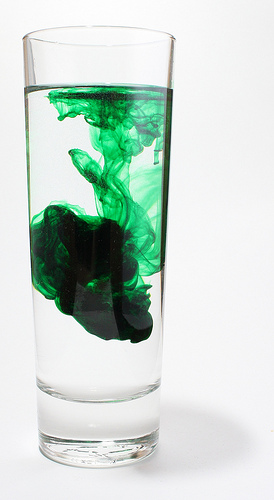
\includegraphics[height=.5\textwidth]{photos/diffusionby-LadyDayDream-flickr.jpg}\par
\textit{Picture by LadyDayDream on Flickr.com}
\end{center}
\end{minipage}
\\
\label{m38736*id10987324}\textbf{Diffusion} is a result of the constant thermal motion of particles. In 1828 Robert Brown observed that pollen grains suspended in water moved about in a rapid, irregular motion. This motion has since become known as \textbf{Brownian motion}. Brownian motion is essentially diffusion of many particles. Brownian motion can also be seen as the random to and fro movement of particles. 
\par 
\label{m38736*id48327}Matter exists in one of three states, namely solid, liquid and gas. A solid has a fixed shape and volume. A liquid takes on the shape of the container that it is in. A gas completely fills the container that it is in. Matter can change between these states by either adding heat or removing heat. This is known as a \textbf{change of state}. As we heat an object (e.g. water) it goes from a solid to a liquid to a gas. As we cool an object it goes from a gas to a liquid to a solid.
The changes of state that you should know are:
\label{m38736*id02341}\begin{itemize}[noitemsep]
\item \textbf{Melting} 
\Definition{ Melting point } {The temperature at which a \textsl{solid} changes its phase or state to become a \textsl{liquid}. The  process is called melting. } 
\item \textbf{Freezing} 
\Definition{Freezing point}{The temperature at which a \textsl{liquid} changes its phase to become a \textsl{solid}. The process is called freezing.}
\item \textbf{Evaporation} \\
Evaporation is the process of going from a liquid to a gas. Evaporation from a liquid's surface can happen at a wide range of temperatures. If more energy is added then bubbles of gas appear inside the liquid and this is known as boiling.
\Definition{  Boiling point } {The temperature at which a \textsl{liquid} changes its phase to become a \textsl{gas}. The process is called evaporation} 
\item \textbf{Condensation} is the process of going from gas to liquid.
\item \textbf{Sublimation} is the process of going from a solid to a gas. The reverse process is called deposition.\end{itemize}
\par \label{m38736*eip-957}If we know the melting and boiling point of a substance then we can say what state (solid, liquid or gas) it will be in at any temperature. \par 
The figure~\ref{fig:PhaseChanges} summarises these processes: \\
    \setcounter{subfigure}{0}
\begin{figure}[H]
\begin{center}
\scalebox{0.8}{
\begin{pspicture}(-2,-2)(15,15)
\SpecialCoor
%\psgrid[gridcolor=lightgray]
\uput[r](-1,1.6){\large{Gas}}
\psline[linewidth=1.5pt]{->}(0.5,2)(4,2)
\uput[r](0.8,2.4){\large{Condensation}}
\uput[r](4.2,1.6){\large{Liquid}}
\psline[linewidth=1.5pt]{->}(6,2)(9.5,2)
\uput[r](6.8,2.4){\large{Freezing}}
\uput[r](9.8,1.6){\large{Solid}}
\psline[linewidth=1.5pt]{<-}(0.5,1)(4,1)
\uput[r](0,0.4){\large{Boiling (or evaporation)}}
\psline[linewidth=1.5pt]{<-}(6,1)(9.5,1)
\uput[r](6.8,0.4){\large{Melting}}
\psline[linewidth=1.5pt]{<-}(0.5,-0.5)(9.5,-0.5)
\uput[r](4,-1){\large{Sublimation}}
\end{pspicture}
}
\caption{Changes in phase}
\label{fig:PhaseChanges}
\end{center}
\end{figure} 

\nopagebreak
\label{m38736*eip-232}
            \begin{f_experiment}{Heating and cooling curve of water}{           
            \label{m38736*eip-860}\noindent{}\textbf{Aim: } To investigate the heating and cooling curve of water. \\
\label{m38736*eip-861}\noindent{}\textbf{Apparatus: } \\
\begin{minipage}{0.25\textwidth}
\begin{itemize}[noitemsep]
 \item beakers
 \item ice
 \item Bunsen burner
 \item thermometer
 \item water
\end{itemize}
\end{minipage}
\begin{minipage}{0.75\textwidth}
% \begin{figure}[H]
 \begin{center}
\scalebox{0.5}
{
  \begin{pspicture}(-5,-5)(5,5)
\psset{unit=1cm}
%\psgrid(0,0)(-5,-5)(5,5)
\newpsstyle{fred} {linestyle=none,fillstyle=solid,fillcolor=cyan}
\newpsstyle{clear} {linestyle=none,fillstyle=solid,fillcolor=white}
%\uput[r](3.5,1){\large{boiling water}}
%\psline[linewidth=0.04]{->}(3.55,1)(2.6,1)
%\uput[r](3.5,3){\large{metal spoon}}
%\psline[linewidth=0.04]{->}(3.55,3)(3,3)
\rput(-4,0){\pstTubeEssais[glassType=becher,niveauLiquide1=20,solide={\pstGrenailleZinc[200]},aspectLiquide1=clear]}
\psline[linewidth=0.1](-4.7,-2)(-2,2)
\psline[linewidth=0.04]{<-}(-2.34,1.5)(-1.5,1.5)
\uput[r](-1.5,1.5){\large{Thermometer}}
\psline[linewidth=0.04]{<-}(-3,-1)(-1.5,-1)
\uput[r](-1.5,-1){\large{Beaker}}
\psline[linewidth=0.04]{<-}(-3.5,-1.5)(-1.5,-1.5)
\uput[r](-1.5,-1.5){\large{Ice}}
\rput(2,0){\pstTubeEssais[glassType=becher,niveauLiquide1=30,aspectLiquide1=fred]}
\psline[linewidth=0.1](1.4,-2)(4,2)
\psline[linewidth=0.04]{<-}(3.7,1.5)(4.5,1.5)
\uput[r](4.5,1.5){\large{Thermometer}}
\psline[linewidth=0.04]{<-}(3,-1)(4.5,-1)
\uput[r](4.5,-1){\large{Beaker}}
\psline[linewidth=0.04]{<-}(2.5,-1.5)(4.5,-1.5)
\uput[r](4.5,-1.5){\large{Water}}
\end{pspicture}
}
 \end{center}
% \end{figure}
\end{minipage} \\ 
\label{m38736*eip-862}\noindent{}\textbf{Method:}
\label{m38736*id9872}\begin{enumerate}[noitemsep, label=\textbf{\arabic*}.]
            \item Place some ice in a beaker.
\item Measure the temperature of the ice and record it.
\item After 1 minute measure the temperature again and record it. Repeat every minute, until at least 3 minutes after the ice has melted.
\item Plot a graph of time versus temperature for the heating of ice.
\item Heat some water in a beaker until it boils. Measure and record the temperature of the water.
\item Remove the water from the heat and measure the temperature every 1 minute, until the beaker is cool to touch.
\end{enumerate}
      \Warning {Be careful when handling the beaker of hot water. Do not touch the beaker with your hands, you will burn yourself.} 
      \label{m38736*eip-863}\noindent{}\textbf{Results: }
\begin{enumerate}[noitemsep, label=\textbf{\arabic*}.]
\item Record your results in the following table: 
          \begin{table}[H]
        \begin{center}
      \label{m38736*uid434}
    \noindent
      \begin{tabular}{|l|l|l|l|}\hline
\multicolumn{2}{|c|}{Heating of ice} & \multicolumn{2}{c|}{Cooling of boiling water}  \\ \hline
 \textbf{Time (min)} & \textbf{Temperature (in $^{\circ} \text{C}$)} &  \textbf{Time (min)} & \textbf{Temperature (in $^{\circ} \text{C}$)} \\ \hline
     0    & & 0    & \\ \hline 
     1    & & 1    & \\ \hline
     2    & & 2    & \\ \hline
     etc. & & etc. & \\ \hline
%           & &      & \\ \hline 
%           & &      & \\ \hline
    \end{tabular}
      \end{center}
\end{table}
\item Plot a graph of time (independent variable, x-axis) against temperature (dependent variable, y-axis) for the ice melting and the boiling water cooling. 
\end{enumerate}
\noindent{}\textbf{Discussion and conclusion: } You should find that the temperature of the ice increases until the first drops of liquid appear and then the temperature remains the same, until all the ice is melted. You should also find that when you cool water down from boiling, the temperature remains constant for a while, then starts decreasing.}
\end{f_experiment} 
 \label{m38736*eip-25}In the above experiment, you investigated the heating and cooling curves of water. We can draw heating and cooling curves for any substance. A \textbf{heating curve} of a substance gives the changes in temperature as we move from a \textsl{solid} to a \textsl{liquid} to a \textsl{gas}. A \textbf{cooling curve} gives the changes in temperature as we move from \textsl{gas} to \textsl{liquid} to \textsl{solid}. An important observation is that as a substance melts or boils, the temperature remains constant until the substance has changed state. This is because all the heat energy goes into breaking or forming the bonds between the molecules. \\
The following diagram gives an example of what heating and cooling curves look like: \\
\begin{minipage}{0.5\textwidth}
\begin{figure}[H]
 \begin{center}
\scalebox{0.3}{
  \begin{pspicture}
\psset{unit=1cm}
\psaxes[linewidth=1.2pt,labels=none,ticks=none]{->}(13,10)
\psline[linewidth=0.1](0,0)(2,2)(4,2)(10,8)(12,8)
\psaxes[linewidth=1.2pt,labels=none,ticks=none]{->}(13,10)
\rput[l]{0}(3,-0.5){\Huge{Time (min)}}
\rput[b]{90}(-0.5,5){\Huge{Temperature ($^{\circ} \text{C}$)}}
   \end{pspicture}
}
\end{center}
\caption{Heating curve}
\end{figure}
\end{minipage}
\begin{minipage}{0.5\textwidth}
\begin{figure}[H]
\begin{center}
\scalebox{0.3}{
  \begin{pspicture}
\psset{unit=1cm}
\psaxes[linewidth=1.2pt,labels=none,ticks=none]{->}(13,10)
\psline[linewidth=0.1](0,8)(2,8)(8,2)(10,2)(12,0)
\psaxes[linewidth=1.2pt,labels=none,ticks=none]{->}(13,10)
\rput[l]{0}(3,-0.5){\Huge{Time (min)}}
\rput[b]{90}(-0.5,5){\Huge{Temperature ($^{\circ} \text{C}$)}}
   \end{pspicture}
}
 \end{center}
\caption{Cooling curve}
\end{figure}
\end{minipage}


         \section{The kinetic molecular theory}
    \nopagebreak
%            \label{m38730} $ \hspace{-5pt}\begin{array}{cccccccccccc}   
\includegraphics[width=0.75cm]{col11305.imgs/summary_video.png} &   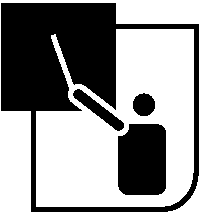
\includegraphics[width=0.75cm]{col11305.imgs/summary_presentation.png} &   \end{array} $ \hspace{2 pt}\raisebox{-5 pt}{} {(section shortcode: P10017 )} \par 
%     \label{m38730*cid5}
%             \subsection{ The Kinetic Theory of Matter}
%             \nopagebreak
      \label{m38730*id308618}The \textbf{kinetic theory of matter} helps us to explain why matter exists in different \textsl{phases} (i.e. solid, liquid and gas), and how matter can change from one phase to the next. The kinetic theory of matter also helps us to understand other properties of matter. It is important to realise that what we will go on to describe is only a \textsl{theory}. It cannot be proved beyond doubt, but the fact that it helps us to explain our observations of changes in phase, and other properties of matter, suggests that it probably is more than just a theory.\\
      \label{m38730*id308641}Broadly, the kinetic theory of matter says that all matter is composed of \textbf{particles} which have a certain amount of \textbf{energy} which allows them to move at different speeds depending on the temperature (energy). There are \textbf{spaces} between the particles and also \textbf{attractive forces} between particles when they come close together.

% \par 
%       \label{m38730*id308647}\begin{itemize}[noitemsep]
%             \label{m38730*uid34}\item Matter is made up of \textbf{particles} that are constantly moving.
% \label{m38730*uid35}\item All particles have \textbf{energy}. Solid particles have the least amount of energy and gas particles have the greatest amount of energy.
% \label{m38730*uid36}\item The \textbf{temperature} of a substance is a measure of the \textsl{average kinetic energy} of the particles.
% \label{m38730*uid37}\item A change in \textbf{phase} may occur when the energy of the particles is changed.
% \label{m38730*uid38}\item There are \textbf{spaces} between the particles of matter.
% \label{m38730*uid39}\item There are \textbf{attractive forces} between particles and these become stronger as the particles move closer together.
% \end{itemize}
      \label{m38730*id308767}Table \ref{tab:microscopic:kinetic theory} summarises the characteristics of the particles that are in each phase of matter.
    % \textbf{m38730*uid40}\par
\begin{table}[h]
\begin{center}

\begin{tabular}{|p{3cm}|p{3cm}|p{3cm}|p{3cm}|}\hline
\textbf{Property of matter} & \textbf{Solid} & \textbf{Liquid} & \textbf{Gas} \\\hline
Particles & Atoms or molecules & Atoms or molecules & Atoms or molecules \\\hline
Energy and movement of particles & Low energy - particles vibrate around a fixed point. & Particles have more energy than in the solid phase but less than in the gas phase. & Particles have high energy and are constantly moving.  \\\hline
Spaces between particles & Very little space between particles. Particles are tightly packed together. & Bigger spaces than in solids but smaller than in gases. & Large spaces because of high energy.  \\\hline
Attractive forces between particles. & Very strong forces. Solids have a fixed volume. & Weaker forces than in solids, but stronger forces than in gases. & Weak forces because of the large distance between particles.  \\\hline
Changes in phase. & Solids become liquids or gases if their temperature is increased. & A liquid becomes a gas if its temperature is increased. A liquid becomes a solid if its temperature decreases. & In general a gas becomes a liquid or solid when it is cooled. Particles have less energy and therefore move closer together so that the attractive forces become stronger, and the gas becomes a liquid or a solid.  \\\hline
\end{tabular}
\caption{Table summarising the general features of solids, liquids and gases.}
\label{tab:microscopic:kinetic theory}
\end{center}
\end{table}
    \par
%       \label{m38730*eip-933}The following presentation is a brief summary of the above. Try to fill in the blank spaces before clicking onto the next slide.
%     \setcounter{subfigure}{0}
% 	\begin{figure}[H] % horizontal\label{m38730*slidesharefigure}
%     \label{m38730*slidesharemedia}\label{m38730*slideshareflash}\raisebox{-5 pt}{ 
\includegraphics[width=0.5cm]{col11305.imgs/summary_www.png}} { (Presentation:  P10018 )} P10016
%  \end{figure}       \par 
\begin{figure}[H]
\begin{center}
\begin{pspicture}(0,0)(10,2.6)
\SpecialCoor
%\psgrid[gridcolor=lightgray]

\rput(0,0.5){\psframe(0,0)(3,2)
\rput(0.1,0){\multirput(0.2,0.2)(0.4,0){7}{\pscircle(0,0){0.2}}
\multirput(0.4,0.55)(0.4,0){6}{\pscircle(0,0){0.2}}
\multirput(0.2,0.9)(0.4,0){7}{\pscircle(0,0){0.2}}}}

\rput(3.5,0.5){\psframe(0,0)(3,2)
\rput(0.2,0.2){\pscircle(0,0){0.2}}
\rput(0.6,0.3){\pscircle(0,0){0.2}}
\rput(1.2,0.3){\pscircle(0,0){0.2}}
\rput(1.7,0.2){\pscircle(0,0){0.2}}
\rput(2.3,0.3){\pscircle(0,0){0.2}}
\rput(2.8,0.2){\pscircle(0,0){0.2}}
\rput(0.3,0.9){\pscircle(0,0){0.2}}
\rput(0.8,0.7){\pscircle(0,0){0.2}}
\rput(1.5,0.8){\pscircle(0,0){0.2}}
\rput(2.0,0.8){\pscircle(0,0){0.2}}
\rput(2.5,0.7){\pscircle(0,0){0.2}}}

\rput(7,0.5){\psframe(0,0)(3,2)
\rput(2.5,0.5){\pscircle(0,0){0.2}}
\rput(2.4,1.7){\pscircle(0,0){0.2}}
\rput(1.5,1){\pscircle(0,0){0.2}}
\rput(0.7,1.7){\pscircle(0,0){0.2}}
\rput(0.3,0.3){\pscircle(0,0){0.2}}}

\uput[d](1.5,0.5){solid}
\uput[d](5,0.5){liquid}
\uput[d](8.5,0.5){gas}

\end{pspicture}
\end{center}
\caption{The three phases of matter}
\label{fig:threephases}
\end{figure}
      \label{m38730*id309053}Taking copper as an example we find that in the solid phase the copper atoms have little energy. They vibrate in fixed positions. The atoms are held closely together in a regular pattern called a \textsl{lattice}. If the copper is heated, the energy of the atoms increases. This means that some of the copper atoms are able to overcome the forces that are holding them together, and they move away from each other to form \textsl{liquid copper}. This is why liquid copper is able to flow, because the atoms are more free to move than when they were in the solid lattice. If the liquid is heated further, it will become a gas. Gas particles have lots of energy and are far away from each other. That is why it is difficult to keep a gas in a specific area! The attractive forces between the particles are very weak. Gas atoms will fill the container they are in. Figure \ref{fig:PhaseChanges} shows the changes in phase that may occur in matter, and the names that describe these processes.\par 
    \setcounter{subfigure}{0}
    
\begin{activity}{The three phases of water}
\begin{minipage}{0.5\textwidth}
Water can be in the form of steam, water liquid or ice. Use marbles (or playdough or clay) to represent water molecules. Arrange the marbles to show the three phases of water. Discuss the properties of each of the phases and the processes and energy in changing from the one phase to the other. 
\end{minipage}
\begin{minipage}{.5\textwidth}
\begin{center}
 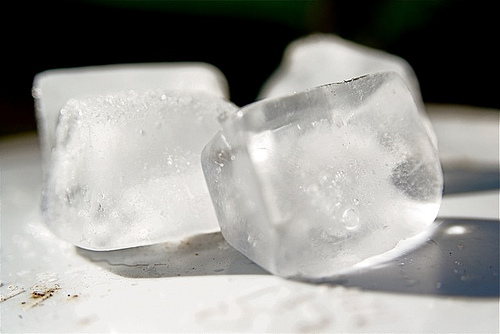
\includegraphics[width=.3\textwidth]{photos/iceby-stevendepolo-flickr.jpg}\par
\textit{Picture by stevendepolo on Flickr.com}
\end{center}
\begin{center}
 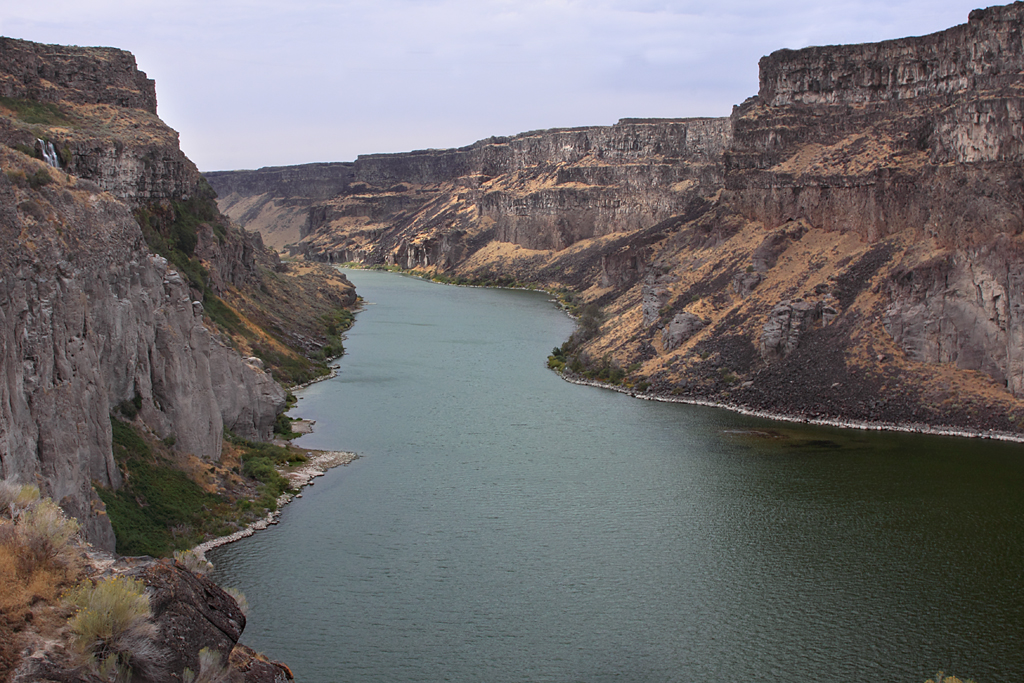
\includegraphics[width=.3\textwidth]{photos/AlanVernon.jpg}\par
\textit{Picture by Alan Vernon on Flickr.com}
\end{center}
\end{minipage}
\end{activity}

      
\label{m38730*cid7}
\summary{VPdgh}
            \nopagebreak
\label{m38730*id311034}\begin{itemize}[noitemsep]
\label{m38730*id973}\item There are three states of matter: solid, liquid and gas.
\label{m38730*id872}\item \textbf{Diffusion} is the movement of particles from a high concentration to a low concentration. Brownian motion is the diffusion of many particles.
\label{m38730*uid83}\item \textbf{Melting point} is the temperature at which a \textsl{solid} changes its phase to become a \textsl{liquid}. The process is called melting.
\item \textbf{Freezing point} is the temperature at which a liquid changes its phase to become a solid. The process is called freezing.
\item Evaporation is the process of going from a liquid to a gas. Evaporation from a liquid’s surface can happen at a wide range of temperatures.
\label{m38730*uid84}\item \textbf{Boiling point} is the temperature at which a liquid changes phase to become a gas. The process is called evaporation. The reverse process (change in phase from gas to liquid) is called \textbf{condensing}.
\item Sublimation is the process of going from a solid to a gas. 
\item The \textbf{kinetic theory of matter} attempts to explain the behaviour of matter in different phases.
\label{m38730*uid81}\item The kinetic theory of matter says that all matter is composed of \textbf{particles} which have a certain amount of \textbf{energy} which allows them to \textbf{move} at different speeds depending on the temperature (energy). There are \textbf{spaces} between the particles and also \textbf{attractive forces} between particles when they come close together.
\end{itemize}
\label{m38730*cid9}
            \begin{eocexercises}{States of matter and the kinetic molecular theory}
            \nopagebreak \noindent
%Question 1
\label{m38730*id311490}\begin{enumerate}[noitemsep, label=\textbf{\arabic*}. ] 
            \label{m38730*uid87}\item Give one word or term for each of the following 
descriptions.
\label{m38730*id311506}\begin{enumerate}[noitemsep, label=\textbf{\alph*}. ] 
            \label{m38730*uid88}\item The change in phase from a solid to a gas.
\label{m38730*uid89}\item The change in phase from liquid to gas.
\end{enumerate}
%Question 2
                \label{m38730*uid103}\item Water has a boiling point of $100 ^{\circ} \text{ C}$
\label{m38730*id311744}\begin{enumerate}[noitemsep, label=\textbf{\alph*}. ] 
            \label{m38730*uid104}\item Define boiling point.
\label{m38730*uid105}\item What change in phase takes place when a liquid reaches its boiling point?
% \label{m38730*uid107}\item Use the kinetic theory of matter and your knowledge of intermolecular forces to explain why water changes phase at this temperature.
\end{enumerate}
%Question 3
\label{m38730*id762}\item Describe a solid in terms of the kinetic molecular theory. \newline
%Question 4
            \label{m38730*uid108}\item Refer to the table below which gives the melting and 
boiling points of a number of elements and then answer the questions that follow. (\textsl{Data from http://www.chemicalelements.com})
    % \textbf{m38730*id311817}\par
          \begin{table}[H]
    % \begin{table}[H]
    % \\ 'id2883166' '1'
        \begin{center}
      \label{m38730*id311817}
      \begin{tabular}{|l|l|l|}\hline
\textbf{Element} & \textbf{Melting point ($^{\circ} \text{C}$)} & \textbf{Boiling point ($^{\circ} \text{C}$)} \\ \hline
        copper &
        1083 &
        2567 \\ \hline
        magnesium &
        650 &
        1107 \\ \hline
        oxygen &
        -218,4 &
        -183 \\ \hline
        carbon &
        3500 &
        4827 \\ \hline
        helium &
        -272 &
        -268,6 \\ \hline
        sulphur &
        112,8 &
        444,6 \\ \hline
    \end{tabular}
      \end{center}
\end{table}
  \label{m38730*id312057}\begin{enumerate}[noitemsep, label=\textbf{\alph*}. ] 
            \label{m38730*uid109}\item What state of matter (i.e. solid, liquid or gas) will each of 
these elements be in at room temperature ($25^{\circ} \text{C}$)?
\label{m38730*uid110}\item Which of these elements has the strongest forces 
between its atoms? Give a reason for your answer.
\label{m38730*uid111}\item Which of these elements has the weakest forces between 
its atoms? Give a reason for your answer.
\end{enumerate}
%Question 5
\item Complete the following submicroscopic diagrams to show what magnesium will look like in the solid, liquid and gas phase.
\begin{figure}[H]
\begin{center}
\scalebox{.8}{
\begin{pspicture}(0,0)(10,2.6)
\SpecialCoor
%\psgrid[gridcolor=lightgray]

\rput(0,0.5){\psframe(0,0)(3,2)}

\rput(3.5,0.5){\psframe(0,0)(3,2)}

\rput(7,0.5){\psframe(0,0)(3,2)}

\uput[d](1.5,0.5){solid}
\uput[d](5,0.5){liquid}
\uput[d](8.5,0.5){gas}

\end{pspicture}
}
\end{center}
\end{figure}
                \end{enumerate}
\label{m38730**end}
\practiceinfo
  \label{3fc6acf7f608d0b0e2d136d6a7710402**end}
\par 
 \par \begin{tabular}[h]{cccccc}
 (1.) lbV  &  (2.) lbp  &  (3.) lgf  &  (4.) lbd  &  (5.) lbv  & \end{tabular}
\end{eocexercises}

%             \chapter{Die atoom}\fancyfoot[LO,RE]{Chemistry: Matter and Materials} 
\label{chap:atom}
%     \setcounter{figure}{1}
%     \setcounter{subfigure}{1}
    \label{ea1c9e59656f96ee804546971cf6dee6}
    \label{m38756*cid1}
            \section{Inleiding}
            \nopagebreak 
%       \par \label{m38756*id254141}
Ons het nou gekyk na die talle voorbeelde van die tipes materie en materiale wat rondom ons bestaan
en ons het sommige van die maniere waarop materiale geklassifiseer word, ondersoek. Waaruit bestaan hierdie materiale nou eintlik en wat maak een materiaal verskillend van 'n ander? Ten einde hierdie vraag te beantwoord, moet ons die boustene van materie, \textbf{atome}, van naderby bekyk. Atome vorm die basis van al die strukture en organismes in die heelal. Die planete, son, gras, bome, lug wat ons inasem en mense is almal opgebou uit verskillende kombinasies van atome.\par 
            

\chapterstartvideo{VPrkk}



\begin{project}{Biblioteek-opdrag: Modelle van die atoom}
            \nopagebreak
            \label{m38756*eip-3}

Ons huidige begrip van die atoom het ontwikkel oor 'n lang tydperk met 'n groot groep verskillende mense wat hierin 'n rol gespeel het. Doen 'n bietjie navorsing oor die ontwikkeling van die verskillende idees oor die atoom en die mense wat bygedra het tot hierdie studie. Sommige mense na wie se werk in hierdie verband gekyk kan word, sluit in: JJ Thomson, Ernest Rutherford, Marie Curie, JC Maxwell, Max Planck, Albert Einstein, Niels Bohr, Lucretius, LV de Broglie, CJ Davison, LH Germer, Chadwick, Werner Heisenberg, Max Born, Erwin Schrodinger, John Dalton, Empedocles, Leucippus,
Democritus, Epicurus, Zosimos, Maria die Jodin, Geber, Rhazes, Robert Boyle, Henry Cavendish, A Lavoisier en H Becquerel. Jy hoef nie inligting oor al hierdie mense te soek nie, maar probeer iets kry oor so veel van hulle as moontlik.
\par \begin{minipage}{.6\textwidth}
\label{m38756*id7342}Maak 'n lys van die belangrikste bydraes wat elkeen van hierdie mense gemaak het tot die opbou van 'n model van die atoom en maak dan 'n tydlyn van hier\-die inligting. (Jy kan 'n aanlynhulpmiddel soos Dipity \textsl(http://www.dipity.com/) gebruik om 'n tydlyn te maak.) Probeer om 'n idee te kry hoe alles uiteindelik bymekaar gevoeg is om ons te bring tot by vandag se moderne begrip van die atoom.
\end{minipage}
\begin{minipage}{.4\textwidth}
 \begin{center}
\textbf{'n Tydlyn van die atoomteorie}
  \includegraphics[height=1.2\textwidth]{photos/timeline_atom.png}
 \end{center}

\end{minipage}

\end{project}
\par \label{m38756*cid2}

\section{Modelle van die atoom}
            \nopagebreak
      \label{m38756*id254164}Dit is belangrik om te besef dat baie van wat ons vandag weet oor die struktuur van atome, ontwikkel het oor 'n lang tydperk. Dit is dikwels hoe wetenskaplike kennis ontwikkel, met een persoon wat voortbou op die idees van iemand anders. Ons gaan kyk hoe ons moderne begrip van die atoom met verloop van tyd ontwikkel het.\par 

\mindsetvid{The origins of atomic theory}{VPakv}

      \label{m38756*id254508}
Die idee van atome is uitgedink deur twee Griekse filosowe, Democritus en Leucippus in die vyfde eeu vC. Die Griekse woord $\alpha \tau o\mu o\nu $ (Atoom) beteken ondeelbaar omdat hulle geglo het dat atome nie in kleiner stukkies gebreek kan word nie.\\
      \label{m38756*id254540}
Vandag weet ons dat atome bestaan uit 'n \textbf{positief} gelaaide kern in die middel omring deur \textbf{negatief gelaaide elektrone}. In die verlede egter, voordat die struktuur van die atoom behoorlik verstaan is, het wetenskaplikes met baie verskillende \textbf{modelle} of \textbf{prente} probeer beskryf hoe atome lyk.

\Definition{Model}{'n Model is 'n voorstelling van 'n stelsel in die werklike wêreld. Modelle help ons om die stelsels en hul eienskappe beter te verstaan. Byvoorbeeld, 'n \textsl{atoommodel} verteenwoordig hoe die struktuur van 'n atoom moontlik \textsl{kan} lyk en is gebaseer op wat ons weet oor die optrede van atome. Dit is nie noodwendig 'n ware beeld van die presiese struktuur van 'n atoom nie.   } 
\subsection*{Dalton se model van die atoom}
\begin{minipage}{.5\textwidth}
John Dalton het voorgestel dat alle materie saamgestel is uit baie klein dele wat hy atome genoem het. Dit was nie 'n totale nuwe konsep nie, aangesien die ou Grieke (veral Democritus) reeds vroeer voorgestel het dat alle materie uit klein, onverdeelbare (kan nie verdeel word nie) eenhede bestaan. Toe Dalton sy model voorgestel het, was die bestaan van iets soos elektrone en die kern nog onbekend. 
\end{minipage}
\begin{minipage}{.5\textwidth}
%    \setcounter{subfigure}{0}
	\begin{figure}[H] % horizontal\label{m38756*uid2}
    \begin{center}
\scalebox{.8}{
\begin{pspicture}(-3,-3)(3,3)
%\psgrid[gridcolor=lightgray]
\pscircle(0,0){1}
\end{pspicture}
}
% \begin{minipage}{.8\textwidth}
\caption{Die atoom volgens Dalton}
% \end{minipage}
% \label{fig:atom:dalton}
\end{center}
 \end{figure}
\end{minipage}

      \label{m38756*uid1}
            \subsection*{Thomson se model van die atoom}
            \nopagebreak
\begin{minipage}{.5\textwidth}
        \label{m38756*id254616}
Na afloop van die ontdekking van die elektron deur J.J. Thomson in 1897, het die mense besef dat atome opgebou is uit nog kleiner deeltjies as wat hulle voorheen gedink het. Die atoomkern was egter nog nie ontdek nie en so is die "Pruimpoeding model" voorgestel in 1904. In hierdie model bestaan die atoom uit negatiewe elektrone wat dryf in  'n “sop” van positiewe ladings, baie soos pruime in 'n poeding of rosyne in 'n vrugtekoek (figuur~\ref{fig:atom:plumpudding}). In 1906 het Thomson die Nobelprys ontvang vir sy werk in hierdie veld. Selfs met die pruimpoeding model was daar nog geen begrip van hoe die elektrone in  'n atoom gerangskik was nie.\\ 
\end{minipage}
\begin{minipage}{.5\textwidth}
%     \setcounter{subfigure}{0}
	\begin{figure}[H] % horizontal\label{m38756*uid2}
    \begin{center}
\scalebox{.7}{
\begin{pspicture}(-3,-3)(3,3)
%\psgrid[gridcolor=lightgray]
\psellipse(0,0)(2.5,2.5)
\psline[linewidth=0.3cm](0,2)(0,-2)
\psline[linewidth=0.3cm](-2,0)(2,0)
\psellipse(-1.5,1.5)(0.25,0.25)
\rput(-1.5,1.5){\textbf{-}}
\psellipse(-1,1)(0.25,0.25)
\rput(-1,1){\textbf{-}}
\psellipse(-1.5,-1)(0.25,0.25)
\rput(-1.5,-1){\textbf{-}}
\psellipse(-1,-1.5)(0.25,0.25)
\rput(-1,-1.5){\textbf{-}}
\psellipse(1,1.5)(0.25,0.25)
\rput(1,1.5){\textbf{-}}
\psellipse(1.5,-1.5)(0.25,0.25)
\rput(1.5,-1.5){\textbf{-}}
\psellipse(1,0.5)(0.25,0.25)
\rput(1,0.5){\textbf{-}}
\psellipse(1,-1)(0.25,0.25)
\rput(1,-1){\textbf{-}}
\psline(1.2,1.6)(3,1.6)
\rput(4,1.6){\textbf{elektrone}}
\psline(2,-1)(3,-1)
\rput(3.8,-1){\textbf{'sop' van}}
\rput(4.3,-1.5){\textbf{positiewe lading}}
\end{pspicture}
}
\begin{minipage}{.8\textwidth}
\caption{Die atoom volgens \\ die pruimpoeding (of rosyntjiekoek) model}
\end{minipage}
\label{fig:atom:plumpudding}
\end{center}
 \end{figure}    
\end{minipage}   
      

\IFact{Twee ander modelle wat voorgestel is vir die atoom, is die kubieke model en die Saturniese model. In die kubieke model is die elektrone voorgestel om hulle te bevind op die hoeke van 'n kubus. In die Saturniese model is daar beskryf dat die elektrone rondom  'n groot, swaar kern sou wentel.}
  
Die ontdekking van \textbf{straling} was die volgende stap op die pad na die opbou van 'n akkurate beeld van atoomstruktuur. In die vroe\"{e} twintigste eeu het Marie Curie en haar man, Pierre, ontdek dat sommige elemente (die \textsl{radio-aktiewe elemente}) deeltjies uitstraal wat in staat is om deur materie te dring op soortgelyke wyse as X-strale (Lees meer hieroor in Graad 11). Dit was Ernest Rutherford wat in 1911 hierdie ontdekking gebruik het om die model van die atoom te hersien.\par 
      

      
            \subsection*{Rutherford se model van die atoom}
            \nopagebreak
\begin{minipage}{.5\textwidth}
            \label{m38756*id254751}
Rutherford het eksperimente uitgevoer wat gelei het tot 'n verandering in die idees rondom die atoom. Sy nuwe model het die atoom beskryf as 'n klein, digte, positief- gelaaide sentrale deel wat die kern genoem is en wat omring is deur die ligter, negatief- gelaaide elektrone.  'n
Ander interpretasie van hierdie model was dat die atoom gesien is as 'n mini-sonnestelsel waar die elektrone rondom die kern wentel
soos planete wat om die son draai. 'n Vereenvoudigde prentjie van hierdie model word getoon in figuur~\ref{fig:atom:rutherfordmodel}. Hierdie model word soms die \textbf{sonnestelsel-model} van die atoom genoem. \par 
\end{minipage}
\begin{minipage}{.5\textwidth}
%     \setcounter{subfigure}{0}
	\begin{figure}[H] % horizontal\label{m38756*uid5}
    \begin{center}
\scalebox{.8}{
\begin{pspicture}(-2.2,-2.4)(2.2,2.4)
\SpecialCoor
%\psgrid%[gridcolor=lightgray]
\def\water{\psset{unit=0.2}\rput{150}{\pscircle[fillcolor=white,fillstyle=solid](0,0){2}
\psarc[fillcolor=white,fillstyle=solid](-1.5,1){1.5}{30}{260}
\psarc[fillcolor=white,fillstyle=solid](1.5,1){1.5}{280}{150}
\rput(-1.5,1){\pscurve(1.5;30)(-1;142.5)(1.5;260)}
\rput(1.5,1){\pscurve(1.5;150)(-1;37.5)(1.5;280)}}}

\def\atom{\rput(0,0){\water}\rput{180}(0.25,0.25){\water}\rput{45}(0.25,0.25){\water}\rput{225}(0.25,0.25){\water}}

\rput(0,0){\atom}
\psellipse[linecolor=lightgray,linewidth=3pt](0,0)(1.5,2.2)
\rput{120}{\psellipse[linecolor=lightgray,linewidth=3pt](0,0)(1.5,2.2)}
\rput{240}{\psellipse[linecolor=lightgray,linewidth=3pt](0,0)(1.5,2.2)}

\psdots[dotsize=5pt](1,1.6)(-1,-1.6)\uput[ur](1,1.6){elektron orbiting the nucleus}
\rput{120}{\psdots[dotsize=5pt](1,1.6)(-1,-1.6)}
\rput{240}{\psdots[dotsize=5pt](1,1.6)(-1,-1.6)}
\uput[r](2.4,0){nucleus}
\psline{<-}(1,0)(2.4,0)
\end{pspicture}
}
\caption{Rutherford se model van die atoom}
\end{center}
\label{fig:atom:rutherfordmodel}
 \end{figure} 
\end{minipage}      
      \label{m38756*uid6}
            \subsection*{Bohr se model van die atoom}
            \nopagebreak
\begin{minipage}{.5\textwidth}
        \label{m38756*id254784}
Daar was egter 'n paar probleme met Rutherford se model: dit kon byvoorbeeld nie die interessante waarneming verklaar dat atome slegs lig uitstraal by sekere golflengtes of frekwensies nie. Niels Bohr het hierdie probleem opgelos deur voor te stel dat die elektrone rondom die kern wentel in sekere spesiale bane by verskillende energievlakke.\\
\end{minipage}
\begin{minipage}{.5\textwidth}
   \setcounter{subfigure}{0}
	\begin{figure}[H] % horizontal\label{m38756*uid2}
    \begin{center}
\scalebox{.5}{
\begin{pspicture}(-6,-6)(6,6)
%\psgrid[gridcolor=lightgray]
\pscircle[fillstyle=solid,fillcolor=gray](0,0){0.1}
\pscircle[linecolor=darkgray,linewidth=0.1](0,0){1}
\pscircle[linecolor=darkgray,linewidth=0.1](0,0){2}
\pscircle[linecolor=darkgray,linewidth=0.1](0,0){3}
\psline[linewidth=0.05]{<-}(0.1,0)(4,0)
\uput[r](4,0){\Large{kern}}
\psline[linewidth=0.05]{<-}(1.8,1)(4,1)
\uput[r](4,1){\Large{elektronbaan}}
\end{pspicture}
}
\begin{minipage}{.8\textwidth}
\caption{Bohr se model van die atoom}
\end{minipage}
\label{fig:atom:dalton}
\end{center}
 \end{figure}
\end{minipage}

\label{m38756*notfhsst!!!underscore!!!id119}
\subsection*{James Chadwick}
Rutherford het voorspel (in 1920) dat 'n ander soort deeltjie saam met die proton teenwoordig moet wees in die kern. Hy het hierdie voorspelling gemaak op grond van die feit dat as daar slegs positief- gelaaide protone in die kern was, dit uitmekaar sou breek as gevolg van die afstotende kragte tussen die soortgelyke ladings van die protone! Om te verseker dat die atoom elektries neutraal bly, moes hierdie deeltjies self neutraal wees. In 1932 het James Chadwick die neutron ontdek en sy massa bepaal.
\label{m38756*eip-279}
            \subsection*{Ander modelle van die atoom}
            \nopagebreak
            \label{m38756*eip-993}
Alhoewel die mees algemene model van die atoom die Bohr-model is, is wetenskaplikes nogsteeds besig om nuwe en verbeterde teorieë te ontwikkel oor die bou van die atoom. Een van die belangrikste bydraes tot atoomteorie (die wetenskaplike studie van atome) was die ontwikkeling van kwantumteorie. Schrödinger, Heisenberg, Born en baie ander het 'n rol gespeel in die ontwikkeling van kwantumteorie. 
\par \label{m38756*eip-179}
            \begin{exercises}{Modelle van die atoom}
{
            \nopagebreak
            \label{m38756*eip-786}Pas die inligting in Kolom A by die belangrikste ontdekker in kolom B.
    % \textbf{m38756*eip-551}\par
          \begin{table}[H]
    % \begin{table}[H]
    % \\ '' '0'
        \begin{center}
      \label{m38756*eip-551}
      \begin{tabular}{|l|l|}\hline
        \textbf{Kolom A} &
        \textbf{Kolom B} \\ \hline
        Ontdekking van elektrone en die pruimpoeding-model & Niels Bohr \\ \hline
        Rangskikking van elektrone & Marie en Pierre Curie  \\ \hline
        Atome as die kleinste boustene van materie & Antieke Grieke \\ \hline
        Die ontdekking van die kern & JJ Thomson \\ \hline
        Die ontdekking van straling & Rutherford \\ \hline
    \end{tabular}
      \end{center}
\end{table}
\vspace{-1cm}
\practiceinfo
 \begin{tabular}[h]{cccccc}
 (1.) 000k  & \end{tabular}
\end{exercises}

            \section{Atoommassa en deursnee}
            \nopagebreak
            \label{m38756*id254850}Dit is soms moeilik om 'n begrip te vorm van die grootte of massa van 'n atoom , want ons kan nie  'n atoom sien nie en ons is ook nie gewoond daaraan om te werk met sulke klein metings nie. 
            \subsection*{Hoe swaar is 'n atoom?}
            \nopagebreak
        \label{m38756*id254863}
Dit is moontlik om die massa van 'n enkele atoom in kilogram te bepaal. Om dit te doen, benodig jy spesiale instrumente en die waardes wat jy sou kry, sou baie lomp wees en ook moeilik om mee te werk. Die massa van 'n koolstofatoom, byvoorbeeld, is ongeveer  $1,99 \times {10}^{-26}\text{ kg}$, terwyl die massa van 'n atoom waterstof ongeveer $1,67 \times {10}^{-27}\text{ kg}$ is. As 'n mens kyk na hierdie baie klein getalletjies, is dit nogal baie moeilik om  'n vergelyking te tref tussen die massas van verskillende atome.\par 
        \label{m38756*id254908}
Om die situasie makliker te maak, gebruik wetenskaplikes 'n ander eenheid vir massa wanneer hulle die massa van  'n atoom beskryf. Hierdie eenheid staan bekend as \textbf{atoommassa-eenhede} (ame). Ons kan hierdie eenheid afkort (verkort) tot slegs "u". Wetenskaplikes gebruik die \textbf{koolstof standaard} om ame te bepaal. Die koolstof-standaard gee koolstof 'n atoommassa van 12 u. In vergelyking met koolstof, sal die massa van 'n waterstofatoom slegs 1 u wees. Jy kan dit kontroleer deur die massa van 'n koolstofatoom in kilogram (sien hierbo) te deel deur deur die massa van 'n waterstofatoom in kilogram (jy sal beslis  'n sakrekenaar hiervoor nodig hê!). As jy die berekening doen, sal jy sien dat die massa van 'n
koolstofatoom twaalf keer groter is as die massa van 'n waterstofatoom. Wanneer ons atoommassa-eenhede gebruik in plaas van kilogram, is dit makliker is om dit raak te sien. Atoommassa-eenhede gee ons dus nie die werklike massa van 'n atoom nie, maar eerder die massa met betrekking tot die massa van een (spesifiek uitgesoekte) atoom in die periodieke tabel. Met ander woorde, dit is slegs 'n syfer in vergelyking met 'n ander syfer. Die belangrikste aspek om hier te onthou, is dat die atoommassa-eenheid relatief is met betrekking tot een (spesifiek uitgesoekte) element. Die atoommassas van sommige elemente word in tabel~\ref{tab:atomic mass} aangetoon.
    % \textbf{m38756*uid8}\par
          \begin{table}[H]
    % \begin{table}[H]
    % \\ '' '0'
        \begin{center}
      \label{m38756*uid8}
    \noindent
      \begin{tabular}{|l|l|}\hline
                  \textbf{Element}
                 &
                  \textbf{Atoommassa (u)}
                \\ \hline
        Koolstof ($\text{C}$) &
        12 \\ \hline
        Stikstof ($\text{N}$) &
        14 \\ \hline
        Broom ($\text{Br}$) &
        80 \\ \hline
        Magnesium ($\text{Mg}$) &
        24 \\ \hline
        Kalium ($\text{K}$) &
        39 \\ \hline
        Kalsium ($\text{Ca}$) &
        40 \\ \hline
        Suurstof ($\text{O}$) &
        16 \\ \hline
    \end{tabular}
      \end{center}
    \caption{Die atoommassagetal van 'n paar van die elemente.}
\label{tab:atomic mass}
\end{table}
    \par
        \label{m38756*id255096}
Die werklike waarde van 1 atoommassa-eenheid is $1,67\ensuremath{\times}{10}^{-24}\phantom{\rule{2pt}{0ex}}\text{g}$ of $1,67\ensuremath{\times}{10}^{-27}\phantom{\rule{2pt}{0ex}}\text{kg}$. Dis 'n baie klein massa! As ons dit uitskryf, lyk dit soos volg: $0,000~000~000~000~000~000~000~000~167~\text{kg}$. 'n Atoom is dus baie, baie klein.
            \subsection*{Rutherford se alfadeeltjie verstrooiing eksperiment}
            \nopagebreak
            \label{m38756*id254668}
Radioaktiewe elemente straal verskillende soorte deeltjies uit. Sommige van hierdie deeltjies is positief gelaaide alfa ($\alpha $)-deeltjies. Rutherford wou uitvind waar presies die positiewe lading in 'n atoom is. Hy het  'n reeks eksperimente uitgevoer waar hy velle bladgoud met alfapartikels bombardeer het.  'n Vereenvoudigde diagram van sy eksperiment word in figuur~\ref{fig:atom:goldfoil} aangetoon. 

\begin{figure}[H] % horizontal\label{m38756*uid4}
 \begin{center}
\scalebox{.7}{
\begin{pspicture}(-4,-3)(9,3)
\SpecialCoor
%\psgrid%[gridcolor=lightgray]

\def\gold{\pscircle(0,0){0.2}\psdot(0,0)}

\rput(0,0){
\psarc[linewidth=2pt](0,0){3}{270}{90}
\psframe[fillcolor=lightgray,fillstyle=solid](-0.2,-2)(0,2)
\psframe[fillcolor=white,fillstyle=solid](-4,-0.5)(-2,0.5)
\rput(-3,0.2){radio-aktiewe}
\uput[d](-3,0.2){bron}
\psline[linewidth=1.5pt]{->}(-2,0)(-0.2,0)
\uput[d](-1.1,0){$\alpha$-deeltjies}
\psline[linestyle=dashed](-0.2,0)(-2,3)
\uput[dr](-1.8,3){C}
\psline[linestyle=dashed](-0.2,0)(-2,-3)
\uput[ur](-1.8,-3){C}

\psline[linestyle=dashed](0,0)(2,2.2)
\uput[l](2,2.2){B}
\psline[linestyle=dashed](0,0)(2,-2.2)
\uput[l](2,-2.2){B}

\psline[linestyle=dashed](0,0)(3,0)
\psline[linestyle=dashed](0,0)(3,0.2)
\uput[ul](3,0.2){A}
\psline[linestyle=dashed](0,0)(3,-0.2)
\uput[dl](3,-0.2){A}

\uput[ur](1.3,-3){Sinksulfiedskerm}}

\rput(5,0){
\psframe(0,-2)(1,2)
\multirput(0.2,-1.8)(0,0.4){10}{\gold}
\multirput(0.5,-1.6)(0,0.4){9}{\gold}
\multirput(0.8,-1.8)(0,0.4){10}{\gold}

\psline{->}(-1,1.5)(2,1.5)\uput[ul](2,1.5){A}
\psline{->}(-1,0.35)(0.5,0.35)(2,0)\uput[ul](2,0){B}
\psline{->}(-1,-1)(0.2,-1)(-1,-2)\uput[u](-1,-2){C}
\pcline[linestyle=none](-1,-2)(-1,2)
\lput*{:U}{$\alpha$-deeltjies}
\psline(0.8,-1.4)(1.4,-1.4)
\rput[l](1.4,-1.4){kern van}
\uput[dr](1.4,-1.5){goudatoom}

}
\rput(-3,-2.5){(a)}
\rput(5.5,-2.5){(b)}
\psline(-0.2,1.5)(-2,1.5)
\rput(-3,1.5){goudblad}
\end{pspicture}
}
\caption{Rutherford se goudblad eksperiment. Figuur (a) toon die pad van die $\alpha$-deeltjies nadat hulle die goudblad getref het. Figuur (b) toon die rangskikking van atome in die goudblad en die pad wat die verskillende $\alpha$-deeltjies volg met betrekking tot die goudblad-atome.}
\label{fig:atom:goldfoil}
\end{center}
\end{figure}       

\mindsetvid{the rutherford model}{VPald}      


Rutherford het sy eksperiment so opgestel dat 'n straal van alfa-partikels gerig was op die goudblaaie. Agter die goudblaaie was 'n skerm gemaak van sinksulfied. Hierdie skerm het Rutherford in staat gestel om te sien waar die alfa-partikels beland het. Rutherford het geweet dat die elektrone in die goud atome nie regtig enige invloed op die pad van die alfa-partikels sou uitoefen nie, omdat die massa van 'n elektron soveel kleiner is as dié van 'n proton. Hy het geredeneer dat dit die positief gelaaide protone sou wees wat die positief gelaaide alfa-partikels sal wegstoot en sodoende hul rigting kan verander.\par 

Wat het hy ontdek het, was dat die meeste van die alfa-partikels ongestoord deur die foelie beweeg het en opgespoor kon word op die skerm direk agter die foelie (A). Sommige van die partikels word effens gedeflekteer na ander dele van die skerm (B). Wat nog meer interessant is, is dat sommige van die deeltjies reguit terug gedeflekteer word in die rigting van waar hulle gekom het (C)! Dit was die deeltjies wat deur die positiewe protone in die goud atome afgestoot is. As die pruimpoeding- model van die atoom waar was, sou Rutherford verwag dat baie meer afstoting sou plaasvind, aangesien die positiewe ladings volgens hierdie model verspreid is oor die hele atoom. Maar dit was nie die geval nie. Die feit dat die meeste deeltjies ongestoord deurbeweeg het, het aangedui dat die positiewe lading slegs gekonsentreer is in een deel van die atoom.\par 

Deur middel van hierdie eksperiment het hy tot die gevolgtrekking gekom dat die kern van die atoom positief gelaai is en gele\"{e} is in die middel van die atoom.
\subsection*{Hoe klein is die kern?}
\begin{minipage}{.5\textwidth}
Die kern van 'n atoom is baie klein. Ons kan die atoom vergelyk met 'n sokkerstadion. As die hele atoom so groot is soos 'n stadion, sal die kern net die grootte van 'n ertjie in die middel van die stadion wees! Dit behoort duidelik te wees dat die atoom hoofsaaklik bestaan uit  'n leë ruimte. As jy al die leë ruimtes verwyder uit die atome in jou liggaam, sou jy die grootte wees van 'n korreltjie sout!
\end{minipage}
\begin{minipage}{.5\textwidth}
\begin{center}
\textbf{'n Stadion}\\
 \includegraphics[width=.4\textwidth]{photos/stadiumby-shine2010-flickr.jpg}\\
\textit{Prent deur Shine 2010 op Flickr.com}
\end{center}
\end{minipage}
      
            \subsection*{Relatiewe atoommassa}
            \nopagebreak
\Definition{Relatiewe atoommassa} {Relatiewe atoommassa is die gemiddelde massa van een atoom van al die isotope van  'n spesifieke chemiese element wat natuurlik voorkom, uitgedruk in atoommassa-eenhede.} 

Die relatiewe atoommassa van 'n element is 'n syfer wat jy op die periodieke tabel sal vind. 

\section{Struktuur van die atoom}
\nopagebreak
\label{m38745*id255206}
As 'n gevolg van die werk wat gedoen is deur vorige wetenskaplikes op atoommodelle (wat ons bespreek het in "modelle van die atoom”), het wetenskaplikes nou 'n goeie idee hoe 'n atoom lyk. Hierdie kennis is belangrik omdat dit ons help om te verstaan ​waarom materie verskillende eienskappe het en waarom sekere materiale met ander verbind. Kom ons bekyk nou die mikroskopiese struktuur van die atoom van naderby. (Hoe die atoom van binne lyk.) \par 

\mindsetvid{the nucleus}{VPaln}

Tot dusver het ons bespreek dat atome bestaan uit 'n positief gelaaide \textbf{kern}, omring deur een of meer negatief gelaaide \textbf{elektrone}. Hierdie elektrone wentel rondom die kern. \par 
      
Voordat ons kyk na 'n paar bruikbare begrippe, moet ons eers verstaan wat elektrone, protone en neutrone is.\par
 
\subsection*{Die Elektron}
\nopagebreak
\label{m38745*id255241}
Die elektron is 'n baie klein deeltjie. Dit het 'n massa van $9,11\ensuremath{\times}{10}^{-31}\phantom{\rule{2pt}{0ex}}\text{kg}$. Wetenskaplikes glo dat die elektron hanteer kan word as \textbf{ 'n deeltjie} of \textbf{element\^{e}re deeltjie} wat beteken dat dit nie opgebreek kan word tot iets kleiner nie. Die elektron dra ook 'n enkele eenheid \textbf{negatiewe} elektriese lading.\par 
\label{m38745*eip-222}
Wat gebeur as 'n atoom elektrone bykry of verloor? Beteken dit dat die atoom nogsteeds deel sal wees van dieselfde element? 'n Verandering in die aantal elektrone van 'n atoom maak nie  'n verskil aan die soort atoom wat dit is nie. Dit sal egter die lading van die atoom verander. Die \textsl{neutraliteit} van die atoom sal verander. As elektrone \textsl{bygevoeg} word, dan word die atoom meer \textsl{negatief} gelaai. Indien elektrone \textsl{weggeneem} word, dan word die atoom meer \textsl{positief} gelaai. Die atoom wat gevorm word in altwee van hierdie gevalle word 'n \textsl{ioon} genoem. 'n Ioon is 'n gelaaide atoom. Byvoorbeeld: 'n neutrale natriumatoom kan 'n elektron verloor en word dan 'n positief gelaaide natriumioon ($\text{Na}^{+}$). 'n Neutrale chlooratoom kan een elektron bykry om 'n negatief gelaaide chloorioon ($\text{Cl}^{-}$) te vorm.
      
\subsection*{Die Kern}
\nopagebreak
\label{m38745*id255305}
In teenstelling met die elektron, \textbf{kan} die kern verdeel word in kleiner boustene naamlik \textbf{protone} en \textbf{neutrone}. Saam word die protone en neutrone \textbf{nukleone} genoem.\par 
        
\subsubsection*{Die Proton}
\nopagebreak
\label{m38745*id255338}
Elke proton dra een eenheid \textbf{positiewe} elektriese lading. Omdat ons weet dat atome \textbf{elektries neutraal} is, m.a.w. dat hulle geen ekstra lading dra nie, moet die aantal protone in 'n atoom dieselfde wees as die aantal elektrone, sodat die positiewe en negatiewe ladings mekaar uitkanselleer. Die totale positiewe lading van 'n kern is gelyk aan die aantal protone in die kern. Die proton is baie swaarder as die elektron (10 000 keer swaarder!) en het 'n massa van $1,6726\ensuremath{\times}{10}^{-27}\phantom{\rule{2pt}{0ex}}\text{kg}$. Wanneer ons praat oor die atoommassa van 'n atoom, word meestal verwys na die gesamentlike massa van die protone en neutrone, dit wil s\^{e}, die nukleone. 

        
\subsubsection*{Die Neutron}
\nopagebreak
\label{m38745*id254468}
Die neutron is elektries neutraal, dit wil s\^{e}, dit dra geen lading nie. Soos die proton, is dit baie swaarder as die elektron en die massa is $1,6749\ensuremath{\times}{10}^{-27}\phantom{\rule{2pt}{0ex}}\text{kg}$ (effens swaarder as die proton).\par 
\label{m38745*notfhsst!!!underscore!!!id214}
    % \textbf{m38745*uid14}\par
          \begin{table}[H]
    % \begin{table}[H]
    % \\ '' '0'
        \begin{center}
      \label{m38745*uid14}
    \noindent
      \begin{tabular}{|l|l|l|l|}\hline
         &
                    \textbf{proton}
                   &
                    \textbf{neutron}
                   &
                    \textbf{elektron} \\ \hline
                    \textbf{Massa (kg)}
                   &
        $1,6726\ensuremath{\times}{10}^{-27}$ &
        $1,6749\ensuremath{\times}{10}^{-27}$ &
        $9,11\ensuremath{\times}{10}^{-31}$ \\ \hline
                    \textbf{Eenhede van lading}
                   &
        $+1$ &
        $0$ &
        $-1$ \\ \hline
                    \textbf{Lading(C)}
                   &
        $1,6 \times {10}^{-19}$ &
        $0$ &
        $-1,6 \times {10}^{-19}$ \\ \hline
    \end{tabular}
      \end{center}
    \caption{Opsomming van die deeltjies binne die atoom}
\end{table}
    
\subsection*{Atoomgetal en atoommassagetal}
\nopagebreak
\label{m38745*id255805}
Die chemiese eienskappe van 'n element word bepaal deur die lading van die kern, dit wil sê deur die \textbf{aantal protone}. Hierdie getal word die \textbf{atoomgetal} genoem en word aangedui deur die letter \textbf{Z}.\par 


\Definition{ Atoomgetal (Z)} {Die aantal protone in 'n atoom } 
      
Jy kan die atoomgetal op die periodieke tabel kry. Die atoomgetal is 'n heelgetal en wissel van 1 tot ongeveer 118.\par 
Die massa van 'n atoom hang af van hoeveel nukleone sy kern bevat. Die aantal nukleone, d.w.s. die totale aantal protone \textbf{plus} neutrone, staan bekend as die \textbf{atoommassagetal} en word aangedui deur die letter \textbf{A}. \par 

\Definition{Atoommassagetal (A)} {Die aantal protone en neutrone in die kern van 'n atoom} 

Die atoomgetal (Z) en die massagetal (A) word aangedui deur gebruik van 'n standaardnotasie, byvoorbeeld, koolstof sal soos volg lyk: $_{6}^{12}\text{C}$.

Standaardnotasie toon die chemiese simbool, die atoommassagetal en die atoomgetal van 'n element as volg:\par 
      
    \setcounter{subfigure}{0}
	\begin{figure}[H] % horizontal\label{m38753*id255893}
    \begin{center}
\scalebox{1} % Change this value to rescale the drawing.
{
\begin{pspicture}(0,-1.2192708)(8.541979,1.2192708)
\usefont{T1}{ptm}{m}{n}
\rput(4.2689586,-0.0765625){\Large $^A_Z$}
\usefont{T1}{ptm}{m}{n}
\rput(4.6527085,-0.0965625){\LARGE $X$}
\psline[linewidth=0.02cm,arrowsize=0.113cm 2.5,arrowlength=1.4,arrowinset=0.0]{->}(3.203646,0.8034375)(4.1636457,0.1034375)
\psline[linewidth=0.02cm,arrowsize=0.113cm 2.5,arrowlength=1.4,arrowinset=0.0]{->}(3.203646,-0.8965625)(4.083646,-0.4165625)
\psline[linewidth=0.02cm,arrowsize=0.113cm 2.5,arrowlength=1.4,arrowinset=0.0]{<-}(4.923646,-0.1165625)(5.8036456,-0.1165625)
\usefont{T1}{ptm}{m}{n}
\rput(7.163802,-0.1065625){\psframebox[linewidth=0.02]{chemiese simbool}}
\usefont{T1}{ptm}{m}{n}
\rput(1.5463021,0.9134375){\psframebox[linewidth=0.02]{aantal nukleone}}
\usefont{T1}{ptm}{m}{n}
\rput(1.6763021,-0.8665625){\psframebox[linewidth=0.02]{aantal protone}}
\end{pspicture} 
}
\end{center}
 \end{figure}       

\Note{'n Nuklied is 'n spesifieke soort atoom of kern wat gekenmerk word deur die aantal protone en neutrone in die atoom. Om presies korrek te wees, moet ons van nukleiede praat wanneer ons te doen het met atome.}
      

Die ysterkern, byvoorbeeld, het 26 protone en 30 neutrone en word aangedui as:
\begin{equation*}
_{26}^{56}\text{Fe}\phantom{\rule{4pt}{0ex}}
\end{equation*}
waar die atoomgetal $Z = 26$ is en die massa getal $A = 56$. Die aantal neutrone is
eenvoudig die verskil tussen die twee $N = A - Z$. \par 

\Tip{Die notasie wat ons gebruik moenie verwar word met die inligting wat op die Periodieke Tabel verskyn nie. Op die Periodieke Tabel verskyn die atoomgetal gewoonlik in die boonste linkerhoek van die blok of direk bokant die element se simbool. Die syfer aan die onderkant van die element se simbool verteenwoordig sy \textbf{relatiewe atoommassa}. Dit is nie presies dieselfde as die atoommassagetal nie. Dit sal verder verduidelik word in die gedeelte oor "Isotope". As voorbeeld verskyn yster se notasie hieronder.
     
 
%     \setcounter{subfigure}{0}
	\begin{figure}[H] % horizontal\label{m38745*id256183}
    \begin{center}
\begin{pspicture}(-2,-2)(2,2)
\psframe(-1,-1)(1,1)
\rput(0,0){\textbf{Fe}}
\rput(-0.7,0.7){26}
\rput(0,-0.7){55.85}
\end{pspicture}
\end{center}
 \end{figure}
}

Een laaste punt oor atoomstruktuur gaan oor die aantal elektrone in 'n atoom. Vir 'n neutrale atoom moet die aantal elektrone dieselfde wees as die aantal protone sodat die lading op die atoom as geheel neutraal sal wees. Wanneer elektrone bygevoeg of verwyder word, sal die atoom nie meer neutraal wees nie. Byvoorbeeld $\text{Li}^{+}$ het een elektron verloor en het nou het slegs 2 elektrone in plaas van 3. $\text{F}^{-}$ het een elektron bygekry en het nou 10 elektrone in plaas van 9.   
\begin{wex}
{%title
Standaardnotasie
}
{%question
Gebruik standaardnotasie om natrium voor te stel en gee die getal protone, neutrone en elektrone in die element.
}
{%Answer
\westep{Gee die element se simbool} $\text{Na}$
\westep{Bepaal die aantal protone} Natrium het 11 protone, so ons het: ${}_{11}\text{Na}$
\westep{Bepaal die aantal elektrone} Natrium is neutraal, so dit het dieselfde aantal elektrone as protone. Die aantal elektrone is 11.
\westep{Bepaal A} Van die periodieke tabel sien ons dat A=23.
\westep{Bereken die aantal neutrone} 
Ons weet wat die waardes van A en Z is, dus kan  ons N bepaal:
$$ \text{N} = \text{A} - \text{Z} = 23 - 11 = 12 $$

\westep{Skryf die antwoord neer} Volgens die standaardnotasie is natrium: $_{11}^{23}\text{Na}$. Die aantal protone is 11, die aantal neutrone is 12. 
}    
\end{wex}
    

\begin{exercises}{Die struktuur van die atoom} \noindent
\begin{enumerate}[noitemsep, label=\textbf{\arabic*}. ] 
\item Verduidelik die betekenis van elk van die volgende terme:
\begin{enumerate}[noitemsep, label=\textbf{\alph*}. ] 
\item kern
\item elektron
\item atoommassa
\end{enumerate}
\item Voltooi die volgende tabel:
% \textbf{m38745*id256298}\par
\begin{center} 
\begin{tabular}{|p{1.4cm}|p{1.4cm}|p{1.4cm}|p{1.4cm}|p{1.4cm}|p{1.4cm}|}\hline
\textbf{Element} & \textbf{Atoom\-massa-eenhede} & \textbf{Atoomgetal} & \textbf{Aantal protone} & \textbf{Aantal elektrone} & \textbf{Aantal neutrone}\\\hline
Mg & 24 & 12 & & & \\\hline
O & & & 8 & & \\\hline
 & & 17 & & & \\\hline
Ni & & & & 28 & \\\hline
 & 40 & & & & 20 \\\hline
Zn & & & & & \\\hline
 & & & & & 0 \\\hline
C & 12 & & & 6 & \\\hline 
$\text{Al}^{3+}$ &  & 13 & & &  \\ \hline
$\text{O}^{2-}$ & & & & 18 &  \\ \hline
\end{tabular}
\end{center}
    \par
          \item Gebruik standaardnotasie om die volgende elemente voor te stel:
\begin{enumerate}[noitemsep, label=\textbf{\alph*}. ] 
            \item kalium
\item koper
\item chloor
\end{enumerate}
                \item 
Vir die element $_{17}^{35}\text{Cl}$, gee die aantal:
\begin{enumerate}[noitemsep, label=\textbf{\alph*}. ] 
            \item protone
\item neutrone
\item elektrone
\end{enumerate}
... in die atoom.\newline
\item Watter van die volgende atome besit 7 elektrone?
\begin{enumerate}[noitemsep, label=\textbf{\alph*}. ] 
            \item $_{2}^{5}\text{He}$
\item $_{6}^{13}\text{C}$
\item $_{3}^{7}\text{Li}$
\item $_{7}^{15}\text{N}$
\end{enumerate}
                \item 
In elk van die volgende gevalle, gee die syfer of die element simbool wat verteenwoordig word deur die "X".
\begin{enumerate}[noitemsep, label=\textbf{\alph*}. ] 
            \item $_{18}^{40}\text{X}$
\item $_{20}^{x}\text{Ca}$
\item $_{x}^{31}\text{P}$
\end{enumerate}
                \item 
Voltooi die volgende tabel:
    % \textbf{m38745*id257121}\par
          \begin{table}[H]
    % \begin{table}[H]
    % \\ 'id2886554' '1'
        \begin{center}
      
    \noindent
      \begin{tabular}{|l|l|l|l|}\hline
         &
        \textbf{A} &
        \textbf{Z} &
        \textbf{N} \\ \hline
        $_{92}^{235}\text{U}$ &
         &
         &
        \\ \hline
        $_{92}^{238}\text{U}$ &
         &
         &
     \\ \hline
    \end{tabular}
      \end{center}
\end{table}
    \par
Vir hierdie twee verskillende vorme van uraan:
\begin{enumerate}[noitemsep, label=\textbf{\alph*}. ] 
            \item Wat is \textsl{dieselfde}?
\item Wat is \textsl{verskillend}?
\end{enumerate}
Uraan kan in verskillende vorme voorkom wat isotope genoem word. Jy sal meer inligting hieroor kry in die gedeelte "Isotope".
\end{enumerate}
  
\practiceinfo
\par 
 \par \begin{tabular}[h]{ccccccc}
 (1.) 000m  &  (2.) 000n  &  (3.) 000p  &  (4.) 000q  &  (5.) 000r  &  (6.) 000s  &  (7.) 000t  & \end{tabular}
\end{exercises}


         \section{Isotope}
    \nopagebreak

Die chemiese eienskappe van 'n element is afhanklik van die aantal protone en elektrone binne die atoom. Indien 'n neutron of twee bygevoeg of verwyder word van die kern, sal die chemiese eienskappe onveranderd bly. Dit beteken dat so 'n atoom se posisie op die Periodieke Tabel dieselfde sal bly. Byvoorbeeld, wanneer enige hoeveelheid neutrone bygevoeg of weggeneem word by  'n kern met 6 protone, sal daardie element nog altyd bekend staan as koolstof met die element simbool $\text{C}$ (raadpleeg die periodieke tabel). Atome wat dieselfde aantal protone besit (d.i. dieselfde atoomgetal Z), maar 'n verskilende getal neutrone (d.i. verskillende N) en daarom verskillende massagetal het, word \textbf{isotope} genoem.\par 

\Definition{Isotope } {Isotope van 'n element het dieselfde aantal protone (dieselfde Z), maar verskillende getal neutrone (verskillende N)} 
        

Die verskillende isotope van 'n element het dieselfde atoomgetal $Z$ maar verskillende atoommassagetalle $A$, want hulle verskil vogens die aantal neutrone $N$. Die chemiese eienskappe van die verskillende isotope van 'n element is dieselfde, maar hulle kan verskil in hoe stabiel hul kerne is. Let daarop dat ons ook elemente kan neerskryf as volg: $E - A$, waar die $E$ die element se simbool is en die $A$ die atoommassa van daardie element. As voorbeeld kyk ons na $\text{Cl}-35$ wat beteken dat chloor 'n atoommassa van $35 ~u$ (17 protone en 18 neutrone) het, terwyl $\text{Cl}-37$ dui op  'n atoomassa van $37 ~u$ (17 protone en 20 neutrone).  \par 

\IFact{Die Griekse woorde $\stackrel{`}{\iota }\sigma o\varsigma \tau \stackrel{`}{o}\pi o\varsigma $ (Isos Topos) beteken ``dieselfde plek''. Dit is waarom atome wat dieselfde aantal protone besit, maar verskil volgens die aantal neutrone, isotope genoem word. Hulle is op dieselfde plek op die periodieke tabel!}

In die natuur wissel die persentasieverspreiding van verskillende isotope.  'n Voorbeeld hiervan is $\text{Cl}-35$ wat tot $75\%$ van alle chlooratome op aarde uitmaak, terwyl die oorblywende $25\%$ $\text{Cl}-37$ is. Die volgende uitgewerkte voorbeeld sal jou wys
hoe om die gemiddelde atoommassa vir hierdie twee isotope te bereken: \par  
\begin{wex}{Die relatiewe atoommassa van 'n isotoop element}{
Die element chloor het twee isotope, chloor-35 en chloor-37. Die verspreiding van hierdie isotope soos dit in die natuur voorkom, is $75\%$ chloor-35 en $25\%$ chloor-37. Bereken die gemiddelde relatiewe atoommassa vir chloor.
}
{
\westep{Bereken die massa bydrae van chloor-35 tot die gemiddelde relatiewe atoommassa}
$75\%$ van die chlooratome het 'n massa van $35~\text{u}$ \\
Bydrae van $\text{Cl-}35 = (\frac{75}{100} \times 35) = 26,25~\text{u}$

\westep{Bereken die bydrae van chloor-37 tot die gemiddelde relatiewe atoommassa}
$25\%$ van die chlooratome het 'n massa van $37~\text{u}$ \\ 
Bydrae van $\text{Cl-}37 = (\frac{25}{100} \times 37) = 9,25~\text{u}$

\westep{Voeg die twee waardes bymekaar om die gemiddelde relatiewe atoommassa van chloor te bepaal}

$\text{Relatiewe atoommassa van chloor} = 26,25~\text{u} + 9,25~\text{u} = 35,5~\text{u}$ \\
}
\end{wex}
As jy op die periodieke tabel kyk (kyk aan die voorkant van die boek), is die gemiddelde relatiewe atoommassa vir chloor is $35,5~\text{u}$. Jy sal oplet dat vir baie elemente die relatiewe atoommassa wat aangedui word, nie 'n heelgetal is nie. Jy behoort nou te verstaan ​dat hierdie getal die \textsl{gemiddelde} relatiewe atoommassa is vir daardie elemente wat natuurlik voorkom as isotope.\par

% Hierdie simulasie stel jou in staat om te sien hoe isotope en relatiewe atoommassa verwant is.

\simulation{Phet simulasie: Isotope}{VPcyv}


\begin{exercises}{Isotopes}
{
\nopagebreak
\begin{enumerate}[noitemsep, label=\textbf{\arabic*}. ] 

\item Atoom A het 5 protone en 5 neutrone en atoom B het 6 protone en 5 neutrone. Hierdie atome is ...
\begin{enumerate}[noitemsep, label=\textbf{\alph*}. ] 
\item allotrope
\item isotope
\item isomere
\item atome van verskillende elemente
\end{enumerate}

\item Vir die swawel isotope, $_{16}^{32}\text{S}$ en $_{16}^{34}\text{S}$, gee die aantal...
\begin{enumerate}[noitemsep, label=\textbf{\alph*}. ] 
\item protone
\item nukleone
\item elektrone
\item neutrone
\end{enumerate}

\item Watter van die volgende is isotope van $_{17}^{35}\text{Cl}$?
\begin{enumerate}[noitemsep, label=\textbf{\alph*}. ] 
\item $_{35}^{17}\text{Cl}$
\item $_{17}^{35}\text{Cl}$
\item $_{17}^{37}\text{Cl}$
\end{enumerate}

\item Watter van die volgende is isotope van die $\text{U-}235$? (X verteenwoordig 'n simbool van 'n element)
\begin{enumerate}[noitemsep, label=\textbf{\alph*}. ] 
\item $_{92}^{238}\text{X}$
\item $_{90}^{238}\text{X}$
\item $_{92}^{235}\text{X}$
\end{enumerate}

\item Voltooi die onderstande tabel:
% \textbf{m38753*id25871115}\par
\begin{center}
\begin{tabular}{|p{2cm}|p{1cm}|p{1cm}|p{1.4cm}|p{1.4cm}|p{1.4cm}|}\hline
\textbf{Isotope} & \textbf{Z} & \textbf{A} & \textbf{Protone} & \textbf{Neutrone} & \textbf{Elektrone}\\\hline
Koolstof-12 & & & & & \\\hline
Koolstof-14 & & & & & \\\hline
Yster-54& & & & & \\\hline
Yster-56 & & & & & \\\hline
Yster-57 & & & & & \\\hline
\end{tabular}
\end{center}

\item As 'n monster $19,9\%$ boor-10 en $80,1\%$ boor-11 bevat, bereken die relatiewe atoommassa van 'n booratoom in daardie monster  

\item As 'n monster $79\%$ Mg-24, $10\%$ Mg-25 en $11\%$ Mg-26 bevat, bereken die relatiewe atoommassa van 'n magnesiumatoom in daardie monster.

\item Vir die element $^{234}_{92}{\text{U}}$ (uraan), gebruik standaardnotasie om die volgende te beskryf:
\begin{enumerate}[noitemsep, label=\textbf{\alph*}. ]
\item die isotoop met 2 neutrone minder
\item die isotoop met 4 neutrone meer
\end{enumerate}

\item Watter van die volgende is isotope van $^{40}_{20}\text{Ca}$?
\begin{enumerate}[noitemsep, label=\textbf{\alph*}. ]
\item $^{40}_{19}\text{K}$
\item $^{42}_{20}\text{Ca}$
\item $^{40}_{18}\text{Ar}$
\end{enumerate}

\item Vir die swawel isotoop $^{33}_{16}\text{S}$, gee die aantal...
\begin{enumerate}[noitemsep, label=\textbf{\alph*}. ]
\item{protone}
\item{nukleone}
\item{elektrone}
\item{neutrone}
\end{enumerate}
\hspace{1ex}        
\end{enumerate}

% Automatically inserted shortcodes - number to insert 10
\par \practiceinfo
\par \begin{tabular}[h]{cccccc}
% Question 1
(1.)	024w	&
% Question 2
(2.)	024x	&
% Question 3
(3.)	024y	&
% Question 4
(4.)	024z	&
% Question 5
(5.)	0250	&
% Question 6
(6.)	0251	\\ % End row of shortcodes
% Question 7
(7.)	0252	&
% Question 8
(8.)	0253	&
% Question 9
(9.)	0254	&
% Question 10
(10.)	0255	&
\end{tabular}
% Automatically inserted shortcodes - number inserted 10
}
\end{exercises}



\section{Elektronkonfigurasie}
\subsection*{Die energie van elektrone}
\nopagebreak
\label{m38741*id259210}
Jy sal onthou uit ons vorige gesprekke dat 'n atoom bestaan uit 'n sentrale kern, bestaande uit protone en neutrone en dat hierdie kern omring word deur elektrone. Alhoewel hierdie elektrone almal dieselfde lading en massa het, verskil die hoeveelheid energie van elke elektron van mekaar. Elektrone met die \textsl{minste} energie beweeg die naaste aan die kern waar die aantrekkingskrag van die positief gelaaide kern die grootste is. Die elektrone met \textsl{meer} energie is in staat om die aantrekkingskrag van die kern te oorkom en word verder weg van die kern gevind.\par 

\mindsetvid{quantisation}{VPama}
\vspace{-1cm}    
\subsection*{Elektronrangskikking}
\nopagebreak
\label{m38741*id9722401}
Ons sal begin met 'n baie eenvoudige beskouing van die rangskikking of konfigurasie van elektrone rondom 'n atoomkern. Hierdie beskouing beskryf eenvoudig dat elektrone in energievlakke (of skille) gerangskik is rondom die kern van  'n atoom. Hierdie energievlakke is genommer 1, 2, 3, ens. Elektrone wat hulle in die eerste energievlak (energievlak 1) bevind, is die naaste aan die kern en sal die minste energie h\^{e}. Elektrone verder weg van die kern sal meer energie besit.\par 
\label{m38741*id259357}In die volgende voorbeelde word die energievlakke getoon as konsentriese sirkels rondom die sentrale kern. Die belangrikste aspek om te onthou rakende hierdie diagramme, is dat die eerste energievlak 2 elektrone kan huisves, terwyl die tweede energievlak 8 elektrone en die derde energievlak ook 8 elektrone kan bevat.\par 
\begin{enumerate}[noitemsep, label=\textbf{\arabic*}. ] 
\item{\textbf{Litium} \\
\begin{minipage}{.4\textwidth}
Litium (Li) het 'n atoomgetal van 3, wat beteken dat in 'n neutrale atoom, die aantal elektrone ook 3 sal wees. Die eerste energievlak bevat twee elektrone, terwyl die derde elektron aangetref word in die tweede energievlak (figuur \ref{fig:atom:lithium}).
\end{minipage}
\begin{minipage}{.6\textwidth}
\begin{figure}[H]
\begin{center}
\scalebox{.7}{
\begin{pspicture}(-5,1)(7,4)
\SpecialCoor
%\psgrid[gridcolor=lightgray]
\rput(0,3){
\pscircle(0,0){1.25}
\pscircle(0,0){0.75}
\pscircle[fillcolor=lightgray,fillstyle=solid](0,0){0.25}
\multido{\n=90+180}{2}{\pscircle[fillcolor=black,fillstyle=solid]({0.75;\n}){0.1}}
\pscircle[fillcolor=black,fillstyle=solid]({1.25;0}){0.1}
\psline(2,0.8)(0.9,0.8)
\uput[r](2,0.8){tweede energievlak}
\psline(2,-0.4)(0.6,-0.4)
\uput[r](2,-0.4){eerste energievlak}
\psline(2,0)({0.75;90})
\psline(2,0)({1.25;0})
\uput[r](2,0){elektrone}
\psline({0.25;-45})(0.8,-1.2)(2,-1.2)
\uput[r](2,-1.2){\parbox[l]{4cm}{kern, met 3 protone en 4 neutrone}}
}
\end{pspicture}
}
\caption{Die rangskikking van\\ elektrone in 'n litiumatoom.}
\label{fig:atom:lithium}
\end{center}
\end{figure}
\end{minipage}
}

\item{\textbf{Fluoor} \\
\begin{minipage}{.4\textwidth}
Fluoor (F) het 'n atoomgetal van 9, wat beteken dat in 'n neutrale atoom daar 9 elektrone sal wees. Die eerste 2 elektrone word gevind in die eerste energievlak, terwyl die ander 7 in die tweede energievlak aangetref word (figuur \ref{fig:atom:fluorine}).
\end{minipage}
\begin{minipage}{.6\textwidth}
\begin{figure}[H]
\begin{center}
\scalebox{1}{
\begin{pspicture}(-5.5,-2)(7,1.5)
\pscircle(0,0){1.25}
\pscircle(0,0){0.75}
\pscircle[fillcolor=lightgray,fillstyle=solid](0,0){0.25}
\multido{\n=90+180}{2}{\pscircle[fillcolor=black,fillstyle=solid]({0.75;\n}){0.1}}
\multido{\n=0+45}{7}{\pscircle[fillcolor=black,fillstyle=solid]({1.25;\n}){0.1}}
\end{pspicture}
}
\caption{Die rangskikking van elektrone in 'n fluooratoom.}
\label{fig:atom:fluorine}
\end{center}
\end{figure}
\end{minipage}
}

\item{\textbf{Neon} \\
\begin{minipage}{.4\textwidth}
Neon (Ne) het 'n atoomgetal van 10, wat beteken dat 'n neutrale atoom 10 elektrone sal bevat. Die eerste 2 elektrone bevind hulle in die eerste energievlak en die ander 8 word in die tweede energievlak aangetref. (figuur \ref{fig:atom:argon}).
\end{minipage}
\begin{minipage}{.6\textwidth}
\begin{figure}[H]
\begin{center}
\scalebox{1.2}{
\begin{pspicture}(-6,-2)(7,2)
% \pscircle(0,0){1.75}
\pscircle(0,0){1.25}
\pscircle(0,0){0.75}
\pscircle[fillcolor=lightgray,fillstyle=solid](0,0){0.25}
\multido{\n=90+180}{2}{\pscircle[fillcolor=black,fillstyle=solid]({0.75;\n}){0.1}}
\multido{\n=0+45}{8}{\pscircle[fillcolor=black,fillstyle=solid]({1.25;\n}){0.1}}
% \multido{\n=0+45}{8}{\pscircle[fillcolor=black,fillstyle=solid]({1.75;\n}){0.1}}
\pscircle[fillcolor=black,fillstyle=solid]({1.25;0}){0.1}
\end{pspicture}
}
\caption{Die rangskikking van elektrone in 'n neonatoom.}
\label{fig:atom:argon}
\end{center}
\end{figure}
\end{minipage}
}
\end{enumerate}


Die situasie is 'n bietjie meer ingewikkeld as wat hier voorgestel word. Binne elke energievlak, beweeg die elektrone in \textbf{orbitale}. 'n Orbitaal definieer die ruimtes of gebiede waar elektrone beweeg.\par 

\Definition{Atoomorbitaal}{'n Atoomorbitaal is die gebied waar 'n elektron gevind kan word om 'n enkele atoomkern.} 
\Note{Elke blokkie in figuur~\ref{fig:Aufbau:blank} kan twee elektrone huisves. Dit beteken dat die s-orbitaal kan twee elektrone huisves, terwyl die p-orbitale in totaal ses elektrone huisves, twee in elk van die drie blokke.}

Die eerste energievlak bevat slegs een s orbitaal, die tweede energievlak bevat een ‘s’orbitaal en drie p orbitale en die derde energievlak bevat een s orbitaal, drie p orbitale (sowel as vyf d orbitale). Binne elke energievlak verteenwoordig die s orbitaal 'n laer energietoestand as die p orbitale. Hierdie rangskikking is getoon in figuur~\ref{fig:Aufbau:blank}. 

\begin{figure}[H]
\begin{center}
 \scalebox{.6}{
 \begin{pspicture}(-6,-8)(6,5)
%\psgrid
 
\rput(-4,0){
% 1s
  \rput(0,-6){ \scalebox{0.5}{	\pspolygon(0,0)(0,2)(3,2)(3,0) }
	\uput[ur](0,1){1s} }
% 2s
  \rput(0,-3){ \scalebox{0.5}{	\pspolygon(0,0)(0,2)(3,2)(3,0) }
	\uput[ur](0,1){2s} }
% 3s
  \rput(0,0){ \scalebox{0.5}{	\pspolygon(0,0)(0,2)(3,2)(3,0) }
	\uput[ur](0,1){3s} }
% 4s
  \rput(0,3){ \scalebox{0.5}{	\pspolygon(0,0)(0,2)(3,2)(3,0) }
	\uput[ur](0,1){4s} }
% 2p
  \rput(2,-2){ \scalebox{0.5}{	\pspolygon(0,0)(0,2)(3,2)(3,0) }
	\uput[ur](0,1){2p} }
  \rput(3.5,-2){ \scalebox{0.5}{	\pspolygon(0,0)(0,2)(3,2)(3,0) }}
  \rput(5,-2){ \scalebox{0.5}{\pspolygon(0,0)(0,2)(3,2)(3,0) }}
% 3p
  \rput(2,1){ \scalebox{0.5}{	\pspolygon(0,0)(0,2)(3,2)(3,0) }	
	\uput[ur](0,1){3p} }
  \rput(3.5,1){ \scalebox{0.5}{\pspolygon(0,0)(0,2)(3,2)(3,0) }}
  \rput(5,1){ \scalebox{0.5}{	\pspolygon(0,0)(0,2)(3,2)(3,0) }}

  \psline(-0.5,-7)(-0.5,5)
  \uput[dr](-2,-1.5){  \scalebox{1.5}{\parbox{\linewidth}{E \\ N \\ E \\ R \\ G \\ I \\ E}} }  
  \uput[u](-1.55,-1){ \psline[doubleline=true, doublesep=3pt]{->}(0,0)(0,3) }

\rput(0,0.5){
\psline(-0.5,-4.25)(7.5,-2.75)
\psline(-0.5,-1.25)(7.5,0.25)
\psline(-0.5,1.75)(7.5,3.25)

\uput[ur](7,-5){ \parbox{\linewidth}{Eerste hoof \\ energievlak} }
\uput[ur](7,-2){ \parbox{\linewidth}{Tweede hoof \\ energievlak} }
\uput[ur](7,1){ \parbox{\linewidth}{Derde hoof \\ energievlak} }
}
}
\end{pspicture}
}
\end{center}
\caption{Die posisies van die eerste tien orbitale van 'n atoom op 'n energievlakdiagram.}
\label{fig:Aufbau:blank}
\end{figure}


Hierdie diagram help ons ook wanneer ons die elektronkonfigurasie van 'n element moet aantoon. Die elektronkonfigurasie van 'n element is die rangskikking van die elektrone in die vlakke en subvlakke. Daar is 'n paar riglyne wat gevolg moet word by die bepaling van die elektronkonfigurasie:
\par 
\begin{itemize}[noitemsep]
\item Elke orbitaal kan slegs \textbf{twee elektrone} huisves. Elektrone wat saam in 'n orbitaal voorkom, staan bekend as  'n \textbf{elektronpaar}.
\item 'n Elektron sal altyd probeer om 'n orbitaal te beset wat die laagste moontlike energie ver\-teen\-woor\-dig.
\item 'n Elektron beset 'n orbitaal eerder op sy eie as om dit te deel met ‘ n ander elektron. 'n Elektron sou eerder ook 'n laer energie orbitaal deel met 'n ander elektron voordat dit sou beweeg na 'n hoër energie-orbitaal. Met ander woorde, binne 'n energievlak word  'n ‘s' orbitaal eers gevul voordat 'p' orbitale gevul word.
\item Die s-subvlak kan 2 elektrone huisves
\item Die p-subvlak kan 6 elektrone huisves
\end{itemize}
In die voorbeelde wat jy gaan hanteer, word s-en p-subvlakke hoofsaaklik gevul.
\par 
Die manier waarop die elektrone in 'n atoom gerangskik is, word sy \textbf{elektronkonfigurasie} genoem.\par 

\Definition{Elektronkonfigurasie}{Elektronkonfigurasie is die rangskikking van elektrone in 'n atoom, molekule of ander fisiese struktuur.} 



\subsection*{Aufbaudiagramme}        
\label{m38741*id259628}

Die elektronkonfigurasie van 'n element kan voorgestel word met behulp van \textbf{Aufbaudiagramme} of energievlakdiagramme. 'n Aufbaudiagram maak gebruik van pyltjies om elektrone voor te stel. Jy kan die volgende stappe volg om jou te help om 'n Aufbaudiagram te teken:\par 
\begin{enumerate}[noitemsep, label=\textbf{\arabic*}. ] 
\item Bepaal die aantal elektrone wat die atoom besit.
\item Vul die 's' orbitaal in die eerste energievlak (die $1\text{s}$ orbitaal) met die eerste twee elektrone.
\item Vul die 's' orbitaal in die tweede energievlak (die $2\text{s}$ orbitaal) met die volgende twee elektrone.
\item Plaas een elektron in elk van die drie 'p' orbitale in die tweede energievlak (die $2\text{p}$ orbitale) en as daar dan nog elektrone oorbly, gaan terug en plaas 'n tweede elektron in elkeen van die $2\text{p}$ orbitale om die elektronpare te voltooi.
\item Gaan voort op hierdie manier deur elk van die opeenvolgende energievlakke totdat al die elektrone geplaas is .
\end{enumerate}

\Tip{As daar twee elektrone in 'n orbitaal is, word dit 'n \textbf{elektronpaar} genoem. As die orbitaal slegs een elektron bevat, word hierdie elektron  'n \textbf{ongepaarde} elektron genoem. Elektronpare word aangetoon met pyltjies wat wys in teenoorgestelde rigtings.}
        
\IFact{Aufbau is die Duitse woord vir 'opbou van'. Wetenskaplikes gebruik hierdie term want dit is presies wat ons doen wanneer ons elektronkonfigurasie uitwerk; ons is besig met die opbou van die atoom se struktuur.}

Jy kan aan Aufbaudiagramme dink as soortgelyk aan die mense wat op 'n bus of trein klim. Mense sal eers gaan sit in die leë sitplekke met ander leë sitplekke oop tussen hulle en die ander mense (tensy hulle mense ken en dan langs hulle gaan sit). Wanneer al die sitplekke op hierdie wyse gevul is, sal enige verdere passasiers gedwing word om langs iemand te staan ​of sit. As die bus of trein vol word, sal nog meer mense moet staan ​om in te pas.\par

 
\subsubsection*{Hund se re\"el en Pauli se beginsel}
\nopagebreak
\label{m38741*eip-188}
Soms verwys mense na Hund se reël vir elektronkonfigurasie. Hierdie reël lui dat elektrone verkies om eerder alleen te verkeer binne ’n subenergievlak as om dit te deel. Dis hoekom wanneer subvlakke gevul word, jy eers net een elektron sal plaas in elk todat elkeen ten minste  'n enkele elektron het en dan eers sal jy voortgaan om  'n tweede elektron daarin te plaas voordat jy aanbeweeg na die volgende energievlak.
\par 

Pauli se uitsluitingsbeginsel sê eenvoudig dat elektrone 'n eienskap vertoon wat bekend staan as spin (rotasie-beweging) en dat twee elektrone in 'n subvlak nie op dieselfde wyse sal spin nie. Dit is waarom ons elektrone voorstel deur twee pyltjies wat in teenoorgestelde rigtings wys.
\par 


\subsection*{Spektroskopiese elektron\-kon\-fig\-u\-ra\-sie\-no\-ta\-sie}
\label{m38741*id259749}
 'n Spesiale tipe notasie word gebruik om 'n atoom se elektronkonfigurasie aan te toon. Hierdie notasie beskryf die energievlakke, orbitale en die aantal elektrone in elke orbitaal. Die elektronkonfigurasie vir litium is byvoorbeeld ${1\text{s}}^{2}{2\text{s}}^{1}$. Die syfer en die letter beskryf die energievlak en die orbitaal en die getal bokant die orbitaal toon hoeveel elektrone in daardie orbitaal is.\\
Aufbaudiagramme vir die elemente fluoor en argon word aangetoon in figuur \ref{fig:Aufbau:fluorine} en figuur \ref{fig:Aufbau:argon} onderskeidelik. Met gebruik van standaard notasie, is die elektronkonfigurasie van fluoor $1\text{s}^{2}{2}\text{s}^{2}2\text{p}^{5}$ en die van argon $1\text{s}^{2}{2}\text{s}^{2}2\text{p}^{5}{3}\text{s}^{2}3\text{p}^{6}$.\\
\begin{minipage}{.5\textwidth}
\begin{figure}[H]
\begin{center}
\scalebox{0.7}{
\begin{pspicture}(-8,-8)(8,5)
%\psgrid
 
 \newpsobject{spin}{psline}{arrowsize=10pt, arrowinset=0, linewidth=3pt}

% 1s
  \rput(0,-5){ \scalebox{0.5}{	\pspolygon(0,0)(0,2)(3,2)(3,0) 
  	\spin{->}(1,0.2)(1,1.8)	\spin{->}(2,1.8)(2,0.2) }
	\uput[ur](0,1){1s} }
% 2s
  \rput(0,-3){ \scalebox{0.5}{	\pspolygon(0,0)(0,2)(3,2)(3,0) 
	\spin{->}(1,0.2)(1,1.8)	\spin{->}(2,1.8)(2,0.2) }
	\uput[ur](0,1){2s} }
% 3s
\rput(0,0){ \scalebox{0.5}{ \pspolygon(0,0)(0,2)(3,2)(3,0) }
	\uput[ur](0,1){3s} }
% 2p
  \rput(2,-2){ \scalebox{0.5}{	\pspolygon(0,0)(0,2)(3,2)(3,0) 
	\spin{->}(1,0.2)(1,1.8)	\spin{->}(2,1.8)(2,0.2) } 
	\uput[ur](0,1){2p} }
  \rput(3.5,-2){ \scalebox{0.5}{	\pspolygon(0,0)(0,2)(3,2)(3,0) 
	\spin{->}(1,0.2)(1,1.8)	\spin{->}(2,1.8)(2,0.2) } }
  \rput(5,-2){ \scalebox{0.5}{\pspolygon(0,0)(0,2)(3,2)(3,0) 	\spin{->}(1,0.2)(1,1.8)}}
% 3p
\rput(2,1){ \scalebox{0.5}{\pspolygon(0,0)(0,2)(3,2)(3,0)}
	\uput[ur](0,1){3p} }
\rput(3.5,1){ \scalebox{0.5}{\pspolygon(0,0)(0,2)(3,2)(3,0)}}
\rput(5,1){ \scalebox{0.5}{ \pspolygon(0,0)(0,2)(3,2)(3,0)}}
\end{pspicture}
}

\caption{ 'n Aufbaudiagram toon die \\  elektronkonfigurasie van fluoor}
\label{fig:Aufbau:fluorine}
\end{center}
\end{figure}
% \end{minipage}


% \begin{minipage}{.45\textwidth}

\begin{figure}[H]
\begin{center}
\scalebox{0.7}{
\begin{pspicture}(-8,-7)(8,4)
%\psgrid
\newpsobject{spin}{psline}{arrowsize=10pt, arrowinset=0, linewidth=3pt}

\rput(-2,0){
% 1s
\rput(0,-5){ \scalebox{0.5}{	\pspolygon(0,0)(0,2)(3,2)(3,0) 
	\spin{->}(1,0.2)(1,1.8)	\spin{->}(2,1.8)(2,0.2) 	}
	\uput[ur](0,1){1s} }
% 2s
\rput(0,-3){ \scalebox{0.5}{	\pspolygon(0,0)(0,2)(3,2)(3,0) 
	\spin{->}(1,0.2)(1,1.8)	\spin{->}(2,1.8)(2,0.2) 	}
	\uput[ur](0,1){2s} }
% 3s
\rput(0,0){ \scalebox{0.5}{		\pspolygon(0,0)(0,2)(3,2)(3,0) 
	\spin{->}(1,0.2)(1,1.8)	\spin{->}(2,1.8)(2,0.2) 	}
	\uput[ur](0,1){3s} }
% 2p
\rput(2,-2){ \scalebox{0.5}{	\pspolygon(0,0)(0,2)(3,2)(3,0) 
	\spin{->}(1,0.2)(1,1.8)	\spin{->}(2,1.8)(2,0.2)	}
	\uput[ur](0,1){2p} }
\rput(3.5,-2){ \scalebox{0.5}{	\pspolygon(0,0)(0,2)(3,2)(3,0) 
	\spin{->}(1,0.2)(1,1.8)	\spin{->}(2,1.8)(2,0.2)	} 	}
\rput(5,-2){ \scalebox{0.5}{	\pspolygon(0,0)(0,2)(3,2)(3,0) 
	\spin{->}(1,0.2)(1,1.8)	\spin{->}(2,1.8)(2,0.2)	}	}
% 3p
\rput(2,1){ \scalebox{0.5}{		\pspolygon(0,0)(0,2)(3,2)(3,0) 
	\spin{->}(1,0.2)(1,1.8)	\spin{->}(2,1.8)(2,0.2)	}
	\uput[ur](0,1){3p} }
\rput(3.5,1){ \scalebox{0.5}{	\pspolygon(0,0)(0,2)(3,2)(3,0) 
	\spin{->}(1,0.2)(1,1.8)	\spin{->}(2,1.8)(2,0.2)	}	}
\rput(5,1){ \scalebox{0.5}{		\pspolygon(0,0)(0,2)(3,2)(3,0) 
	\spin{->}(1,0.2)(1,1.8)	\spin{->}(2,1.8)(2,0.2)	}	}
}
\end{pspicture}
}

\caption{ 'n Aufbaudiagram toon \\ die elektronkonfigurasie van argon}
\label{fig:Aufbau:argon}
\end{center}
\end{figure}
\end{minipage}
\Tip{
Die spektroskopiese elektronkonfigurasie kan geskryf word in  'n korter vorm. Hierdie vorm word geskryf as [edelgas] elektrone, waar die edelgas die naaste een is wat net voor die spesifieke element voor kom. Magnesium kan byvoorbeeld geskryf word as $\text{[Ne]}3\text{s}^{2}$ en koolstof as $\mathrsf{[H]}2\text{s}^{2}2\text{p}^{2}$. Dit staan bekend as die verkorte elektronkonfigurasie.}
\begin{wex}
{%title
Aufbaudiagramme en spektroskopiese elektronkonfigurasie
}
{%question
Gee die elektronkonfigurasie vir stikstof ($\text{N}$) en teken 'n Aufbaudiagram.
}
{%answer
\westep{Gee die aantal elektrone} Stikstof het 7 elektrone.
\westep{Plaas twee elektrone in die $1\text{s}$ orbitaal} Ons begin deur die plaas van twee elektrone in die $1\text{s}$ orbitaal: ${1\text{s}}^{2}$. 
\begin{figure}[H]
\scalebox{0.7}{
 \begin{pspicture}(-8,-6)(8,-2)
%\psgrid
\pspolygon[lincolor=black,fillstyle=solid,fillcolor=white](-2.5,-5.5)(-2.5,-3.2)(0,-3.2)(0,-5.5)
 \newpsobject{spin}{psline}{arrowsize=10pt, arrowinset=0, linewidth=3pt}
\rput(-2,0){
  \rput(0,-5){ \scalebox{0.5}{	\pspolygon(0,0)(0,2)(3,2)(3,0) 
  	\spin{->}(1,0.2)(1,1.8)	\spin{->}(2,1.8)(2,0.2) }
	\uput[ur](0,1){1s} }
}
\end{pspicture}
}
\label{fig:Aufbau:wex}
\end{figure}
Nou het ons 5 elektrone oor om nog te plaas in die orbitale.
\westep{Plaas twee elektrone in die $2\text{s}$ orbitaal} 
Ons het twee elektrone in die $2\text{s}$ orbitaal: ${2\text{s}}^{2}$. 
    %\setcounter{subfigure}{0}
\begin{figure}[H]
\scalebox{0.7}{
 \begin{pspicture}(-8,-6)(8,-2)
%\psgrid
\pspolygon[lincolor=black,fillstyle=solid,fillcolor=white](-2.5,-5.5)(-2.5,-1.2)(0,-1.2)(0,-5.5)
 \newpsobject{spin}{psline}{arrowsize=10pt, arrowinset=0, linewidth=3pt}
\rput(-2,0){
% 1s
  \rput(0,-5){ \scalebox{0.5}{	\pspolygon(0,0)(0,2)(3,2)(3,0) 
  	\spin{->}(1,0.2)(1,1.8)	\spin{->}(2,1.8)(2,0.2) }
	\uput[ur](0,1){1s} }
% 2s
  \rput(0,-3){ \scalebox{0.4}{	\pspolygon(0,0)(0,2)(3,2)(3,0) 
	\spin{->}(1,0.2)(1,1.8)	\spin{->}(2,1.8)(2,0.2) }
	\uput[ur](0,1){2s} }
}
\end{pspicture}
}
\label{fig:Aufbau:wex1}
\end{figure}    
Daar is nou 3 elektrone oor om in orbitale te plaas.
\westep{Plaas drie elektrone in die $2\text{p}$ orbitaal}
Ons plaas 3 elektrone in die $2\text{p}$ orbitaal: ${2\text{p}}^{3}$.
\begin{figure}[H]
\scalebox{.7}{
 \begin{pspicture}(-8,-8)(8,5)
%\psgrid
\pspolygon[lincolor=black,fillstyle=solid,fillcolor=white](-4.5,-5.5)(-4.5,0)(14,0)(14,-5.5) 
 \newpsobject{spin}{psline}{arrowsize=10pt, arrowinset=0, linewidth=3pt}
%1st p elektron
\rput(-4,0){
% 1s
  \rput(0,-5){ \scalebox{0.4}{	\pspolygon(0,0)(0,2)(3,2)(3,0) 
  	\spin{->}(1,0.2)(1,1.8)	\spin{->}(2,1.8)(2,0.2) }
	\uput[ur](0,1){1s} }
% 2s
  \rput(0,-3){ \scalebox{0.4}{	\pspolygon(0,0)(0,2)(3,2)(3,0) 
	\spin{->}(1,0.2)(1,1.8)	\spin{->}(2,1.8)(2,0.2) }
	\uput[ur](0,1){2s} }
% 2p
  \rput(1.8,-2){ \scalebox{0.4}{\pspolygon(0,0)(0,2)(3,2)(3,0) 
	\spin{->}(1,0.2)(1,1.8)	 } 
	\uput[ur](0,1){2p} }
  \rput(3,-2){ \scalebox{0.4}{ \pspolygon(0,0)(0,2)(3,2)(3,0) 
		 } }
  \rput(4.2,-2){ \scalebox{0.4}{\pspolygon(0,0)(0,2)(3,2)(3,0) }}}
%second p elektron
\rput(2,0){
% 1s
  \rput(0,-5){ \scalebox{0.4}{	\pspolygon(0,0)(0,2)(3,2)(3,0) 
  	\spin{->}(1,0.2)(1,1.8)	\spin{->}(2,1.8)(2,0.2) }
	\uput[ur](0,1){1s} }
% 2s
  \rput(0,-3){ \scalebox{0.4}{	\pspolygon(0,0)(0,2)(3,2)(3,0) 
	\spin{->}(1,0.2)(1,1.8)	\spin{->}(2,1.8)(2,0.2) }
	\uput[ur](0,1){2s} }
% 2p
  \rput(1.8,-2){ \scalebox{0.4}{\pspolygon(0,0)(0,2)(3,2)(3,0) 
	\spin{->}(1,0.2)(1,1.8)	 } 
	\uput[ur](0,1){2p} }
  \rput(3,-2){ \scalebox{0.4}{ \pspolygon(0,0)(0,2)(3,2)(3,0) 
	\spin{->}(1,0.2)(1,1.8)	 } }
  \rput(4.2,-2){ \scalebox{0.4}{\pspolygon(0,0)(0,2)(3,2)(3,0) }}}
%3rd p elektron
\rput(8,0){
% 1s
  \rput(0,-5){ \scalebox{0.4}{	\pspolygon(0,0)(0,2)(3,2)(3,0) 
  	\spin{->}(1,0.2)(1,1.8)	\spin{->}(2,1.8)(2,0.2) }
	\uput[ur](0,1){1s} }
% 2s
  \rput(0,-3){ \scalebox{0.4}{	\pspolygon(0,0)(0,2)(3,2)(3,0) 
	\spin{->}(1,0.2)(1,1.8)	\spin{->}(2,1.8)(2,0.2) }
	\uput[ur](0,1){2s} }
% 2p
  \rput(1.8,-2){ \scalebox{0.4}{\pspolygon(0,0)(0,2)(3,2)(3,0) 
	\spin{->}(1,0.2)(1,1.8)	 } 
	\uput[ur](0,1){2p} }
  \rput(3,-2){ \scalebox{0.4}{ \pspolygon(0,0)(0,2)(3,2)(3,0) 
	\spin{->}(1,0.2)(1,1.8)	 } }
  \rput(4.2,-2){ \scalebox{0.4}{\pspolygon(0,0)(0,2)(3,2)(3,0) \spin{->}(1,0.2)(1,1.8) }}
}
\end{pspicture}
}
\label{fig:Aufbau:wex2}
\end{figure}
\westep{Skryf die finale antwoord} Die elektronkonfigurasie is: ${1\text{s}}^{2}{2\text{s}}^{2}{2\text{p}}^{3}$. Die Aufbaudiagram is gegee in die laaste stap hierbo.
} 
\end{wex} 
\subsubsection*{Aufbaudiagramme vir ione}
Wanneer 'n neutrale atoom 'n elektron verloor, word dit positief gelaai en ons noem dit 'n katioon. As natrium byvoorbeeld een elektron verloor, word $\text{Na}^{+}$ gevorm en as kalsium twee elektrone verloor, word $\text{Ca}^{2+}$ gevorm. In elk van hierdie gevalle sal dit die buitenste elektrone wees wat verwyder word.\\
Wanneer 'n neutrale atoom 'n elektron bykry, word dit negatief gelaai en ons noem dit 'n anioon. Chloor sal byvoorbeeld een elektron bykry en $\text{Cl}^{-}$ word gevorm terwyl suurstof twee elektrone sal bykry om $\text{O}^{2-}$ te vorm. \\
Aufbaudiagramme en elektronkonfigurasies kan vir katione sowel as anione uitgewerk word. Die volgende uitgewerkte voorbeeld sal jou wys hoe dit gedoen word.
\begin{wex}
{%title
Aufbaudiagram vir 'n ioon
}
{%question
Gee die elektronkonfigurasie vir ($\text{O}^{2-}$) en teken 'n Aufbaudiagram.
}
{%answer
\westep{Noem die aantal elektrone} Suurstof het 8 elektrone. Die suurstof anioon het twee elektrone bygekry en dus is die totale aantal elektrone 10.
\westep{Plaas twee elektrone in die $1\text{s}$ orbitaal} Ons begin deur die plaas van twee elektrone in die $1\text{s}$ orbitaal: ${1\text{s}}^{2}$. 
\begin{figure}[H]
\scalebox{0.7}{
 \begin{pspicture}(-8,-6)(8,-2)
%\psgrid
\pspolygon[lincolor=black,fillstyle=solid,fillcolor=white](-2.5,-5.5)(-2.5,-3.2)(0,-3.2)(0,-5.5)
 \newpsobject{spin}{psline}{arrowsize=10pt, arrowinset=0, linewidth=3pt}
\rput(-2,0){
  \rput(0,-5){ \scalebox{0.5}{	\pspolygon(0,0)(0,2)(3,2)(3,0) 
  	\spin{->}(1,0.2)(1,1.8)	\spin{->}(2,1.8)(2,0.2) }
	\uput[ur](0,1){1s} }
}
\end{pspicture}
}
\label{fig:Aufbau:wex}
\end{figure}
Nou het ons 8 elektrone oor om te plaas in orbitale.  
\westep{Plaas twee elektrone in die $2\text{s}$ orbitaal} 
Ons het twee elektrone in die $2\text{s}$ orbitaal: ${2\text{s}}^{2}$. 
    \setcounter{subfigure}{0}
\begin{figure}[H]
\scalebox{0.7}{
 \begin{pspicture}(-8,-6)(8,-2)
%\psgrid
\pspolygon[lincolor=black,fillstyle=solid,fillcolor=white](-2.5,-5.5)(-2.5,-1.2)(0,-1.2)(0,-5.5)
 \newpsobject{spin}{psline}{arrowsize=10pt, arrowinset=0, linewidth=3pt}
\rput(-2,0){
% 1s
  \rput(0,-5){ \scalebox{0.5}{	\pspolygon(0,0)(0,2)(3,2)(3,0) 
  	\spin{->}(1,0.2)(1,1.8)	\spin{->}(2,1.8)(2,0.2) }
	\uput[ur](0,1){1s} }
% 2s
  \rput(0,-3){ \scalebox{0.5}{	\pspolygon(0,0)(0,2)(3,2)(3,0) 
	\spin{->}(1,0.2)(1,1.8)	 }
	\uput[ur](0,1){2s} }
}
\end{pspicture}
}
\label{fig:Aufbau:wex1}
\end{figure}    
Daar is nou 6 elektrone oor om in orbitale te plaas.
\westep{Plaas 6 elektrone in die $2\text{p}$ orbitaal}
Ons plaas 6 elektrone in die $2\text{p}$ orbitaal: ${2\text{p}}^{6}$.
\westep{Write the final answer} Die elektronkonfigurasie is: ${1\text{s}}^{2}{2\text{s}}^{2}{2\text{p}}^{6}$. Die Aufbaudiagram sal soos volg lyk:
\begin{figure}[H]
\scalebox{.7}{
 \begin{pspicture}(-8,-8)(8,5)
%\psgrid
\pspolygon[lincolor=black,fillstyle=solid,fillcolor=white](-2.5,-5.5)(-2.5,0)(5,0)(5,-5.5) 
 \newpsobject{spin}{psline}{arrowsize=10pt, arrowinset=0, linewidth=3pt}
\rput(-2,0){
% 1s
  \rput(0,-5){ \scalebox{0.5}{	\pspolygon(0,0)(0,2)(3,2)(3,0) 
  	\spin{->}(1,0.2)(1,1.8)	\spin{->}(2,1.8)(2,0.2) }
	\uput[ur](0,1){1s} }
% 2s
  \rput(0,-3){ \scalebox{0.5}{	\pspolygon(0,0)(0,2)(3,2)(3,0) 
	\spin{->}(1,0.2)(1,1.8)	\spin{->}(2,1.8)(2,0.2) }
	\uput[ur](0,1){2s} }
% 2p
  \rput(2,-2){ \scalebox{0.5}{	\pspolygon(0,0)(0,2)(3,2)(3,0) 
	\spin{->}(1,0.2)(1,1.8)	\spin{->}(2,1.8)(2,0.2) } 
	\uput[ur](0,1){2p} }
  \rput(3.5,-2){ \scalebox{0.5}{ \pspolygon(0,0)(0,2)(3,2)(3,0) 
	\spin{->}(1,0.2)(1,1.8)	\spin{->}(2,1.8)(2,0.2) } }
  \rput(5,-2){ \scalebox{0.5}{\pspolygon(0,0)(0,2)(3,2)(3,0) \spin{->}(1,0.2)(1,1.8) \spin{->}(2,1.8)(2,0.2)}}
}
\end{pspicture}
}
\label{fig:Aufbau:wex2}
\end{figure}
} 
\end{wex} 

\subsection*{Orbitaalfatsoene}
\noindent
\label{m38741*eip-793}
Daar is verskillende orbitaal fatsoene (vorms), maar ons sal hoofsaaklik te doene kry met slegs twee. Dit is die 's'en 'p' orbitale (Daar is ook 'd' en 'f' orbitale). Die 's' orbitale is bolvormig (sferies) en die "p" orbitale is dubbeltraanvormig.
    \setcounter{subfigure}{0}
	\begin{figure}[H] % horizontal\label{m38741*id8245}
\begin{center}
\begin{pspicture}(0,-1.5567888)(6.108,1.5567888)
\definecolor{color634}{rgb}{0.41568627450980394,0.4588235294117647,0.49411764705882355}
\definecolor{color634f}{rgb}{0.23137254901960785,0.23137254901960785,0.25098039215686274}
\definecolor{color695b}{rgb}{0.4235294117647059,0.43137254901960786,0.49411764705882355}
\definecolor{color692b}{rgb}{0.7333333333333333,0.7333333333333333,0.7333333333333333}
\definecolor{color692}{rgb}{0.6862745098039216,0.7098039215686275,0.7254901960784313}
\psbezier[linewidth=0.016,linecolor=color634,fillstyle=gradient,gradlines=2000,gradbegin=color634,gradend=color634f,gradmidpoint=0.52](1.9839575,0.27360383)(1.5600004,1.1712114)(2.68,1.1161642)(2.334384,0.29892722)(1.9887681,-0.5183097)(2.11399,-0.12744273)(1.9403774,-0.71702397)(1.7667648,-1.3066052)(2.6060376,-1.2972081)(2.3922937,-0.72241354)(2.1785495,-0.14761904)(2.4079146,-0.62400377)(1.9839575,0.27360383)
\pscircle[linewidth=0.0020,linecolor=color692,dimen=outer,fillstyle=solid,fillcolor=color692b](0.44,-0.1487886){0.44}
\pscircle[linewidth=0.0020,linecolor=color695b,dimen=outer,fillstyle=solid,fillcolor=color695b](0.44,-0.1487886){0.4}
\psbezier[linewidth=0.016,linecolor=color634,fillstyle=gradient,gradlines=2000,gradbegin=color634,gradend=color634f,gradmidpoint=0.52](4.9417176,0.09809867)(6.1,0.4780618)(5.9620123,-0.63795465)(4.9522166,-0.2531433)(3.9424214,0.13166805)(4.427838,-0.012347225)(3.6947043,0.18963116)(2.9615707,0.39160955)(2.9220605,-0.44713286)(3.6602473,-0.261493)(4.398434,-0.07585315)(3.7834356,-0.28186443)(4.9417176,0.09809867)
\psbezier[linewidth=0.016,linecolor=color634,fillstyle=gradient,gradlines=2000,gradbegin=color634,gradend=color634f,gradmidpoint=0.52](4.8482184,-0.23489222)(5.978085,-0.8157982)(5.081038,-1.4687886)(4.6059003,-0.47938454)(4.130762,0.51001954)(4.3883357,0.06203622)(3.988259,0.7281589)(3.5881824,1.3942816)(2.9616313,0.85712796)(3.6414664,0.44879168)(4.3213015,0.040455382)(3.7183516,0.34601378)(4.8482184,-0.23489222)
\psbezier[linewidth=0.016,linecolor=color634,fillstyle=gradient,gradlines=2000,gradbegin=color634,gradend=color634f,gradmidpoint=0.52](4.228985,0.42143404)(3.7991445,1.5487888)(4.920202,1.4554945)(4.5794764,0.44523695)(4.238751,-0.5650206)(4.3616085,-0.08095095)(4.191572,-0.81145567)(4.021536,-1.5419605)(4.861285,-1.5487885)(4.6438103,-0.82814765)(4.4263353,-0.10750665)(4.658826,-0.7059207)(4.228985,0.42143404)
\end{pspicture} 
    \end{center}
\caption{Die orbitaalvorms. Van links na regs: 'n s-orbitaal, 'n P-orbitaal, en drie p-orbitale}
\label{fig:orbitals}
 \end{figure}     
   \IFact{Wanneer ons orbitale teken, teken ons 'n fatsoen met 'm grens (d.i. die geslote vorm). Dit verteenwoordig die afstand van die kern, waarby ons 'n 95\% sekerte het om elektrone te kry. In werklikheid kan die elektrone van 'n atoom enige afstand weg van die kern af gevind word.}         


\subsection*{Kern- en valenselektrone}
\nopagebreak
\label{m38741*id259935}
Elektrone in die buitenste energievlak van 'n atoom word \textbf{valenselektrone} genoem. Die elektrone wat in die energievlakke nader aan die kern is, word \textbf{kernelektrone} genoem. Kern-elektrone is al die elektrone in 'n atoom, met uitsondering van die valenselektrone. 'n Element met  'n valensie-energievlak wat gevul is, is meer \textbf{stabiel} en \textsl{minder geneig om te reageer} as ander elemente met 'n valensie-energievlak wat nie vol is nie.\par 

\Definition{Valenselektrone} { Die elektrone in die buitenste energievlak van 'n atoom} 

\Definition{Kernelektrone} {Al die elektrone in 'n atoom, met die uitsondering van die valenselektrone}
\begin{exercises}{Valens en kern elektrone}
{
Voltooi die voglende tabel:
 \begin{center}
  \begin{tabular}{|l|l|l|l|} \hline
   \textbf{Element of Ioon} & \textbf{Elektronkonfigurasie} & \textbf{Kernelektrone} & \textbf{Valenseelektrone} \\ \hline
   Kalium ($\text{K}$) & & & \\ \hline
   Helium ($\text{He}$) & & & \\ \hline
   Stuurstof ioon ($\text{O}^{2-}$) & & & \\ \hline
   Magnesium ioon ($\text{Mg}^{2+}$) & & & \\ \hline
  \end{tabular}
 \end{center}

% Automatically inserted shortcodes - number to insert 1
\par \practiceinfo
\par \begin{tabular}[h]{cccccc}
% Question 1
(1.)	0256	&
\end{tabular}
% Automatically inserted shortcodes - number inserted 1
}
\end{exercises}
      

\subsection*{Die belangrikheid om elektronkonfigurasie te verstaan}
\nopagebreak
\label{m38741*id260011}
Teen hierdie tyd kan jy wonder waarom dit belangrik is vir jou om te verstaan hoe elektrone rondom die kern van 'n atoom gerangskik is. Onthou dat in chemiese reaksies, wanneer atome in aanraking kom met mekaar, is dit die elektrone van die atome wat eerste in aanraking kom met mekaar. Meer spesifiek dit is die \textbf{valenselektrone} van die atome wat sal bepaal hoe hulle met mekaar reageer.\par 
        
Om neem dit 'n stap verder; 'n atoom is mees stabiel (en dus \textsl{onreaktief}) wanneer al die orbitale vol is. Aan die ander kant, 'n atoom is die minste stabiel (en dus \textsl{mees reaktief}) wanneer sy valenselektron-orbitale nie vol is nie. Dit sal meer sin maak as ons gaan kyk na die chemiese binding in 'n latere hoofstuk. Om dit eenvoudig te stel, die valenselektrone is grootliks verantwoordelik vir 'n element se chemiese gedrag en elemente wat dieselfde aantal valenselektrone het, toon dikwels soortgelyke chemiese eienskappe.\par 

Die mees stabiele konfigurasies is die voorbeelde waar die energievlakke vol is. Hierdie konfigurasies kom voor in die edelgasse. Die edelgasse is baie stabiele elemente wat nie maklik reageer (indien enigsins) met ander elemente nie. Dit is as gevolg van die vol energievlakke. Alle elemente streef na die mees stabiele elektronkonfigurasie, d.w.s. alle elemente wil soos edelgasse wees. Hierdie beginsel van stabiliteit word ook soms na verwys as die oktetreël. 'n Oktet is 'n stel van 8, en die aantal elektrone in 'n vol energie vlak is 8. \par 

\mindsetvid{colourful cations}{VPamk}

\nopagebreak
\begin{i_experiment}{Vlamtoetse}{
\nopagebreak
\textbf{Doel:}\newline
Om die vlamkleur van 'n metaalkatioon te bepaal.\\
\textbf{Apparaat:}\newline
\begin{minipage}{.5\textwidth}
\begin{itemize}[noitemsep]
\item horlosieglas
\item Bunsenbrander
\item metanol
\item tandestokkie (of sosatiestokkies)
\item metaalsoute (bv. $\text{NaCl}$, ${\text{CuCl}}_{2}$, ${\text{CaCl}}_{2}$, $\text{KCl}$, ens.)
\item metaalpoeiers (bv. koper, magnesium, sink, yster, ens.)
\end{itemize}
\end{minipage}
\begin{minipage}{.5\textwidth}
\begin{center}
 \includegraphics[width=.8\textwidth]{photos/offbeatcin.jpg}\par
\textit{Foto deur offbeatcin op Flickr.com}
\end{center}
\end{minipage}
\Warning{Wees versigtig wanneer jy met 'n bunsenbrander werk, want jy kan maklik jouself verbrand. Maak seker dat alle serpe/loshangende klere veilig ingesteek is en maak lang hare vas. Let daarop dat jy in 'n goed geventileerde ruimte moet werk en dat daar niks vlambaar naby die oop vlam kom nie.}
\textbf{Metode:}\newline
Met elke sout of poeier doen jy die volgende: 
\begin{enumerate}[noitemsep, label=\textbf{\arabic*}. ] 
\item Doop 'n skoon tandestokkie in die metanol.
\item Doop die tandestokkie in die sout of poeier.
\item Beweeg die tandestokkie deur die vlam van die Bunsenbrander. MOENIE die tandestokkie in die vlam hou nie,
maar beweeg dit liewers heen en weer deur die vlam.
\item Neem waar wat gebeur
\end{enumerate}
\textbf{Resultaat:}\newline
Teken jou resultate in 'n tabel aan; dui die metaalsout en die kleur van die vlam aan.
\\ 
\textbf{Gevolgtrekking:}\newline
Jy behoort waar te neem dat die verskillende metaalsoute en poeiers wat jy gebruik het, elkeen met 'n verskillende kleur vlam brand.}
\end{i_experiment}
Die bostaande eksperiment rakende vlamtoetse hou verband met die lynemissiespektra van metale. Hierdie lynemissiespektra is 'n direkte gevolg van die rangskikking van die elektrone in metale. Elke metaalsout brand met 'n unieke kleur vlam. \par 

\begin{exercises}{Energie diagramme en elektrone}
{
\nopagebreak
\begin{enumerate}[noitemsep, label=\textbf{\arabic*}. ] 
\item Teken Aufbaudiagramme om die elektronkonfigurasie van elk van die volgende elemente aan te toon:
\begin{enumerate}[noitemsep, label=\textbf{\alph*}. ] 
\item magnesium
\item kalium
\item swawel
\item neon
\item stikstof
\end{enumerate}
\item Gebruik die Aufbaudiagramme wat jy getrek het om jou te help om die volgende tabel te voltooi:
\begin{center}
\begin{tabular}{|p{1.6cm}|p{2.6cm}|p{2.6cm}|p{2.6cm}|}\hline
\textbf{Element} & \textbf{Aantal energievlakke} & \textbf{Aantal elektrone}  & \textbf{Elektronkonfigurasie (standaardnotasie)}\\\hline
$\text{Mg}$ & &  & \\\hline
$\text{K}$ & &  & \\\hline
$\text{S}$ & & & \\\hline
$\text{Ne}$ &  & & \\\hline
$\text{N}$ & & & \\\hline
$\text{Ca}^{2+}$ & & & \\\hline
$\text{Cl}^{-}$ & & & \\\hline
\end{tabular}
\end{center}    

\item Rangskik die elemente wat hierbo gebruik word in volgorde van toenemende reaktiwiteit. Gee redes vir die keuse van jou volgorde..
\end{enumerate}

% Automatically inserted shortcodes - number to insert 3
\par \practiceinfo
\par \begin{tabular}[h]{cccccc}
% Question 1
(1.)	0257	&
% Question 2
% (2.)	0258	&
% % Question 3
% (3.)	0259	&
\end{tabular}
% Automatically inserted shortcodes - number inserted 3
}
\end{exercises}            

Vroe\"{e}r in hierdie hoofstuk het ons gepraat oor die verskillende "modelle" van die atoom. In die wetenskap is een van die gebruike van modelle dat hulle ons kan help om die struktuur van iets wat ons nie kan sien nie, te verstaan. In die geval van die atoom, help modelle ons om 'n prentjie vir onsself op te bou van hoe die atoom lyk.\par 

Modelle is dikwels vereenvoudig. Die klein karretjies waarmee jy as kind gespeel het, is modelle. Hulle gee jou 'n goeie idee van hoe 'n ware motor lyk, maar hulle is baie kleiner en baie eenvoudiger. 'n Model kan nie altyd heeltemal akkuraat wees nie en dit is belangrik dat ons dit besef sodat ons nie die verkeerde idee hieroor opbou nie.\par 
\begin{groupdiscussion}{Die bou van 'n model van 'n atoom}
\nopagebreak
% \begin{minipage}{.6\textwidth}
\begin{multicols}{2}
In groepe van 3-4 gaan jy 'n model van 'n atoom bou. Elke groep kry 'n ander element om voor te stel. Voordat jy begin, dink oor die volgende vrae:\par 
\begin{itemize}[noitemsep]
\item Watter inligting het ek oor die struktuur van die atoom? (Bv. Uit watter dele is dit opgebou? Hoe groot is dit?)
\item Watter materiaal kan ek gebruik om hierdie dele so akkuraat as moontlik voor te stel?
\item Hoe kan ek al hierdie verskillende dele saamvoeg in my model?
\end{itemize}

Deel jou idees in die groep en beplan dan hoe jy die model sal bou. Sodra die model klaar gebou is, bespreek die volgende vrae:\par 
\begin{itemize}[noitemsep]
\item Is ons model 'n goeie weergawe van hoe die atoom werklik lyk?
\item In watter mate is ons model nie akkuraat nie? Ons weet byvoorbeeld dat elektrone rondom die atoom se kern beweeg, maar in jou model is dit dalk nie moontlik gewees om dit aan te toon nie.
\item Is daar enige manier waarop ons model verbeter kan word?
\end{itemize}

Kyk nou wat die ander groepe gedoen het. Bespreek dieselfde vrae vir elk van die modelle wat jy waarneem en skryf die antwoorde neer. \par 
\end{multicols}
% \end{minipage}
% \begin{minipage}{.4\textwidth}
\begin{center}
\textbf{Bou 'n atoom}\\
 \includegraphics[width=0.4\textwidth]{photos/BuildAtom.png}
\end{center}

% \end{minipage}
\end{groupdiscussion}   

\simulation{PhET simulation for building atoms}{VPcmk}
\simulation{Simulation for building atoms 2}{VPcph}   
    \label{m38741*cid10}
\summary{VPcre}
\nopagebreak
\begin{itemize}[noitemsep]
\item Baie van wat ons vandag weet oor die atoom, is die resultaat van die studie van 'n groot aantal wetenskaplikes wat aangesluit het by mekaar se werk om vir ons 'n goeie begrip te gee van atoomstruktuur.
\item Sommige van die belangrikste wetenskaplike bydraers sluit in \textbf{JJ Thomson} (ontdekking van die elektron, wat gelei het tot die rosyntjiekoekmodel van die atoom), \textbf{Ernest Rutherford} (ontdekking dat positiewe lading in die middel van die atoom gekonsentreer is) en \textbf{Niels Bohr} (die rangskikking van elektrone rondom die kern in energievlakke).
\item As gevolg van die baie klein massa van atome, is die massa gemeet in \textbf{atoommassa-eenhede} (A). $1\phantom{\rule{2pt}{0ex}}u=1,67\ensuremath{\times}10{}^{-24}\phantom{\rule{2pt}{0ex}}\text{g}$.
\item 'n Atoom bestaan uit 'n sentrale kern (bevat \textbf{protone} en \textbf{neutrone}) wat omring word deur \textbf{elektrone}.
\item Die \textbf{atoomgetal} (Z) is die aantal protone in 'n atoom.
\item Die \textbf{atoommassagetal} (A) is die aantal protone en neutrone in die kern van 'n atoom.
\item Die \textbf{standaardnotasies} wat gebruik word om 'n element neer te skryf, is $_{Z}^{A}\text{X}$, waar X is die simbool van die element, A is die atoommassa en Z is die atoomgetal.
\item Die \textbf{isotoop} van 'n spesifieke element is saamgestel uit atome wat dieselfde aantal protone het as die atome in die oorspronklike element, maar verskil volgens die aantal neutrone. Dit beteken dat nie alle atome van 'n element dieselfde atoommassa het nie.
\item Die \textbf{relatiewe atoommassa} van 'n element is die gemiddelde massa van een atoom van al die isotope van 'n spesifieke chemiese element wat natuurlik voorkom, uitgedruk in atoommassa eenhede. Die relatiewe atoommassa word geskryf onder die simbool van die elemente op die periodieke tabel.
% \item The energy of elektrons in an atoom is \textbf{quantised}. Electrons occur in specific energievlaks around an atom's nucleus.
\item Binne elke energievlak, kan 'n elektron beweeg binne 'n bepaalde ruimte of \textbf{orbitaal}. 'n Orbitaal definieer die ruimte waarbinne 'n elektron waarskynlik te vinde is. Daar is verskillende orbitaalvorms, insluitend s, p, d en f orbitale.
\item Energie diagramme soos \textbf{Aufbaudiagramme} word gebruik om die elektronkonfigurasie van die atoom te toon.
\item Die elektrone in die buitenste energievlak word \textbf{valenselektrone} genoem.
\item Die elektrone wat nie valenselektrone is nie, word \textbf{kernelektrone} genoem.
\item Atome waar die heel buitenste energievlak vol is, is minder chemies reaktief en daarom meer stabiel as dié atome waarvan die buitenste energievlak nie vol is nie.
\end{itemize}

\pagebreak
\begin{eocexercises}{Die atoom}
            \nopagebreak
      \begin{enumerate}[noitemsep, label=\textbf{\arabic*}. ] 
            \item Skryf slegs die woord / term vir elk van die volgende beskrywings neer.
\begin{enumerate}[noitemsep, label=\textbf{\alph*}. ] 
            \item Die som van die aantal protone en neutrone in 'n atoom.
\item Die gedefinieerde ruimte om 'n atoom se kern, waar 'n elektron mees waarskynlik te vinde is.
\end{enumerate}
                \item Vir elk van die volgende, sê of die stelling Waar of Vals is. As dit Onwaar is, skryf die korrekte weergawe van die stelling neer.
\begin{enumerate}[noitemsep, label=\textbf{\alph*}. ] 
            \item $_{10}^{20}\text{Ne}$ en $_{10}^{22}\text{Ne}$ het elk 10 protone, 12 elektrone en 12 neutrone.
\item Die atoommassa van 'n atoom van 'n spesifieke element is altyd dieselfde.
\item Dit is veiliger om heliumgas eerder as waterstofgas in ballonne te gebruik.
\item Groep 1 elemente vorm geredelik negatiewe ione.
\end{enumerate}
                \item Die drie basiese komponente van 'n atoom is:
\begin{enumerate}[noitemsep, label=\textbf{\alph*}. ] 
          
% \begin{enumerate}[noitemsep, label=\textbf{\alph*}. ] 
            \item protone, neutrone, en ione
\item protone, neutrone en elektrone
\item protone, neutrinos en ione
\item protium, deuterium en tritium
\end{enumerate}
                \item Die lading van 'n atoom is:
\begin{enumerate}[noitemsep, label=\textbf{\alph*}. ] 
            \item positief
\item neutraal
\item negatief
\item geeneen van die bogenoemde
\end{enumerate}
                \item As Rutherford neutrone gebruik het in plaas van alfapartikels in sy verstrooiing eksperiment, sou die neutrone:
\begin{enumerate}[noitemsep, label=\textbf{\alph*}. ] 
            \item nie deflekteer/buig nie, want hulle het geen lading nie
\item meer dikwels gedeflekteer het
\item maklik tot die kern aangetrek gewees het
\item dieselfde resultate gegee het
\end{enumerate}

\item Beskou die isotoop $_{92}^{234}\text{U}$. Watter een van die volgende stellings is \textsl{waar}?
\begin{enumerate}[noitemsep, label=\textbf{\alph*}. ] 
\item Die element is 'n isotoop van $_{94}^{234}\text{Pu}$
\item Die element bevat 234 neutrone
\item Die element het dieselfde elektronkonfigurasie as $_{92}^{238}\text{U}$
\item Die element het 'n atoommassa getal van 92
\end{enumerate}
\item Die elektronkonfigurasie van 'n atoom van chloor kan voorgestel word deur gebruik te maak van die volgende notasie:
\begin{enumerate}[noitemsep, label=\textbf{\alph*}. ] 
\item  ${1\text{s}}^{2}{2\text{s}}^{8}{3\text{s}}^{7}$
\item ${1\text{s}}^{2}{2\text{s}}^{2}{2\text{p}}^{6}{3\text{s}}^{2}{3\text{p}}^{5}$
\item ${1\text{s}}^{2}{2\text{s}}^{2}{2\text{p}}^{6}{3\text{s}}^{2}{3\text{p}}^{6}$
\item ${1\text{s}}^{2}{2\text{s}}^{2}{2\text{p}}^{5}$
\end{enumerate}
                
        \item Gee die standaardnotasie vir die volgende elemente:
\begin{enumerate}[noitemsep, label=\textbf{\alph*}. ] 
 \item berillium
\item koolstof-12
\item titanium-48
\item fluoor
\end{enumerate}
\item Gee die elektronkonfigurasies en Aufbaudiagramme vir die volgende elemente:
\begin{enumerate}[noitemsep, label=\textbf{\alph*}. ] 
            \item aluminium
\item fosfor
\item koolstof
\item suurstofioon
\item kalsiumioon
\end{enumerate}
\item Vir elk van die volgende elemente gee die aantal protone, neutrone en elektrone in die element: 
\begin{enumerate}[noitemsep, label=\textbf{\alph*}. ] 
\item $_{78}^{195}\text{Pt}$
\item $_{18}^{40}\text{Ar}$
\item $_{27}^{59}\text{Co}$
\item $_{3}^{7}\text{Li}$
\item $_{5}^{11}\text{B}$
\end{enumerate}
\item Vir elk van die volgende elemente gee die element of syfer verteenwoordig deur x: \begin{enumerate}[noitemsep, label=\textbf{\alph*}. ] 
            \item $_{45}^{103}\text{X}$
\item $_{x}^{35}\text{Cl}$
\item $_{4}^{x}\text{Be}$
\end{enumerate}
\item Watter van die volgende is isotope van $_{12}^{24}\text{Mg}$:
\begin{enumerate}[noitemsep, label=\textbf{\alph*}. ] 
            \item $_{25}^{12}\text{Mg}$
\item $_{12}^{26}\text{Mg}$
\item $_{13}^{24}\text{Al}$
\end{enumerate}
\item As 'n monster $69\%$ of koper-63 en $31\%$ of koper-65 bevat, bereken die relatiewe atoommassa van 'n atoom van daardie monster.
            \item Voltooi die volgende tabel:
    % \textbf{m38741*eip-282}\par
          \begin{table}[H]
    % \begin{table}[H]
    % \\ 'id2892806' '1'
        \begin{center}
      
    \noindent
      \begin{tabular}{|l|l|l|l|}\hline
        Element of ioon &
        Elektronkonfigurasie &
        Kernelektrone &
        Valenselektrone \\ \hline
        Boor ($\text{B}$) &
         &
         &
       \\ \hline
        Kalsium ($\text{Ca}$) &
         &
         &
     \\ \hline
        Silikon ($\text{Si}$) &
         &
         &
       \\ \hline
        Litiumioon ($\text{Li}^{+}$) &
         &
         &
      \\ \hline
        Neon ($\text{Ne}$) &
         &
         &
     \\ \hline
    \end{tabular}
      \end{center}
\end{table}
    \par
\end{enumerate}

\practiceinfo
\begin{tabular}[h]{cccccc}
 (1.) 025a  &  (2.) 025b  &  (3.) 025c  &  (4.) 025d  &  (5.) 025e  &  (6.) 025f  &  (7.) 025g  &  (8.) 025h  &  (9.) 025i  &  (10.) 025j  &  (11.) 025k  &  (12.) 025m  &  (13.) 025n  &  (14.) 025p  &  & &  &
\end{tabular}

\end{eocexercises}

%               \chapter{The periodic table}\fancyfoot[LO,RE]{Chemistry: Matter and materials}
    \setcounter{figure}{1}
    \setcounter{subfigure}{1}
 \label{m38760*cid9}
            \section{The arrangement of the elements}
            \nopagebreak
%            \label{m38760} $ \hspace{-5pt}\begin{array}{cccccccccccc}   \includegraphics[width=0.75cm]{col11305.imgs/summary_video.png} &   \end{array} $ \hspace{2 pt}\raisebox{-5 pt}{} {(section shortcode: P10025 )} \par 
      \label{m38760*id261491}The \textbf{periodic table of the elements} is a method of showing the chemical elements in a table with the elements arranged in order of increasing atomic number. Most of the work that was done to arrive at the periodic table that we know can be attributed to a Russian chemist named \textbf{Dmitri Mendeleev}. Mendeleev designed the table in 1869 in such a way that recurring ("periodic") trends or patterns in the properties of the elements could be shown. Using the trends he observed, he left gaps for those elements that he thought were 'missing'. He also predicted the properties that he thought the missing elements would have when they were discovered. Many of these elements were indeed discovered and Mendeleev's predictions were proved to be correct.\par 
\chapterstartvideo{VParg}
      \label{m38760*id261511}To show the recurring properties that he had observed, Mendeleev began new rows in his table so that elements with similar properties were in the same vertical columns, called \textbf{groups}. Each row was referred to as a \textbf{period}. Figure~\ref{fig:atom:periodic} shows a simplified version of the periodic table. The full periodic table is reproduced at the front of this book. You can view an online periodic table at \textsl{http://periodictable.com/}. \par 
    \setcounter{subfigure}{0}
	\begin{figure}[H] % horizontal\label{m38760*uid133}
 \begin{center}
\begin{pspicture}(-7.8,-1)(6.8,4)
%\psgrid[gridcolor=gray]
\psset{unit=0.75}
\pspolygon[fillstyle=solid,fillcolor=teal](-9,3)(-9,4)(-8,4)(-8,3)(-9,3)
\pspolygon[fillstyle=solid,fillcolor=gray](-9,0)(-9,3)(-8,3)(-7,3)(-7,1)(3,1)(3,2)(4,2)(4,0)(-9,0)
\pspolygon[fillstyle=solid,fillcolor=cyan](3,2)(3,3)(4,3)(4,2)(3,2)
\pspolygon[fillstyle=solid,fillcolor=cyan](4,0)(4,2)(5,2)(5,1)(6,1)(6,0)(4,0)
\pspolygon[fillstyle=solid,fillcolor=teal](5,2)(4,2)(4,3)(8,3)(8,4)(9,4)(9,0)(6,0)(6,1)(5,1)(5,2)
\psline(-8,3)(-8,0)
\psline(-7,1)(-7,0)
\psline(-6,1)(-6,0)
\psline(-5,1)(-5,0)
\psline(-4,1)(-4,0)
\psline(-3,1)(-3,0)
\psline(-2,1)(-2,0)
\psline(-1,1)(-1,0)
\psline(0,1)(0,0)
\psline(1,1)(1,0)
\psline(2,1)(2,0)
\psline(3,1)(3,0)
\psline(5,3)(5,2)
\psline(5,1)(5,0)
\psline(6,3)(6,1)
\psline(7,3)(7,0)
\psline(8,3)(8,0)
\psline(-9,3)(-8,3)
\psline(-9,2)(-7,2)
\psline(-9,1)(9,1)
\psline(5,2)(9,2)
\psline(8,3)(9,3)
\rput(-8.5,3.5){\textbf{H}}
\rput(-8.5,2.5){\textbf{Li}}
\rput(-8.5,1.5){\textbf{Na}}
\rput(-8.5,0.5){\textbf{K}}
\rput(-7.5,2.5){\textbf{Be}}
\rput(-7.5,1.5){\textbf{Mg}}
\rput(-7.5,0.5){\textbf{Ca}}
\rput(-6.5,0.5){\textbf{Sc}}
\rput(-5.5,0.5){\textbf{Ti}}
\rput(-4.5,0.5){\textbf{V}}
\rput(-3.5,0.5){\textbf{Cr}}
\rput(-2.5,0.5){\textbf{Mn}}
\rput(-1.5,0.5){\textbf{Fe}}
\rput(-0.5,0.5){\textbf{Co}}
\rput(0.5,0.5){\textbf{Ni}}
\rput(1.5,0.5){\textbf{Cu}}
\rput(2.5,0.5){\textbf{Zn}}
\rput(3.5,2.5){\textbf{B}}
\rput(3.5,1.5){\textbf{Al}}
\rput(3.5,0.5){\textbf{Ga}}
\rput(4.5,2.5){\textbf{C}}
\rput(4.5,1.5){\textbf{Si}}
\rput(4.5,0.5){\textbf{Ge}}
\rput(5.5,2.5){\textbf{N}}
\rput(5.5,1.5){\textbf{P}}
\rput(5.5,0.5){\textbf{As}}
\rput(6.5,2.5){\textbf{O}}
\rput(6.5,1.5){\textbf{S}}
\rput(6.5,0.5){\textbf{Se}}
\rput(7.5,2.5){\textbf{F}}
\rput(7.5,1.5){\textbf{Cl}}
\rput(7.5,0.5){\textbf{Br}}
\rput(8.5,3.5){\textbf{He}}
\rput(8.5,2.5){\textbf{Ne}}
\rput(8.5,1.5){\textbf{Ar}}
\rput(8.5,0.5){\textbf{Kr}}
\psline[linewidth=0.1,arrows=<->](-9.5,4)(-9.5,0)
\pcline[linestyle=none](-9.5,0)(-9.5,4)
\aput{:U}{Period}
\rput(-8.5,5){group number}
\rput(-8.5,4.6){1}
\rput(-7.5,3.5){2}
\rput(3.5,3.5){13}
\rput(4.5,3.5){14}
\rput(5.5,3.5){15}
\rput(6.5,3.5){16}
\rput(7.5,3.5){17}
\rput(8.5,4.5){18}
\psline[linewidth=0.1,arrows=->](-7,-0.5)(5,-0.5)
\pcline[linestyle=none](-7,-0.5)(5,-0.5)
\bput{:U}{Group}
\end{pspicture}
\end{center}
\caption{A simplified diagram showing part of the periodic table. Metals are given in gray, metalloids in light blue and non-metals in turquoise.}
\label{fig:atom:periodic}
 \end{figure}       
            
\subsection*{Definitions and important concepts}
Before we can talk about the trends in the periodic table, we first need to define some terms that are used:
\begin{itemize}[noitemsep]
\item \textbf{Atomic radius} \\
The atomic radius is a measure of the size of an atom. 
\item \textbf{Ionisation energy}\\
The first ionisation energy is the energy needed to remove one electron from an atom in the gas phase. The ionisation energy is different for each element. We can also define second, third, fourth, etc. ionisation energies. These are the energies needed to remove the second, third, or fourth electron respectively. 
\item \textbf{Electron affinity}\\
Electron affinity can be thought of as how much an element wants electrons.
\item \textbf{Electronegativity}\\
Electronegativity is the tendency of atoms to attract electrons. The electronegativity of the elements starts from about 0.7 (Francium ($\text{Fr}$)) and goes up to 4 (Fluorine ($\text{F}$))
\item A \textbf{group} is a vertical column in the periodic table and is considered to be the most important way of classifying the elements. If you look at a periodic table, you will see the groups numbered at the top of each column. The groups are numbered from left to right starting with 1 and ending with 18. This is the convention that we will use in this book. On some periodic tables you may see that the groups are numbered from left to right  as follows: 1, 2, then an open space which contains the \textbf{transition elements}, followed by groups 3 to 8. Another way to label the groups is using Roman numerals.
\item A \textbf{period} is a horizontal row in the periodic table of the elements. The periods are labelled from top to bottom, starting with 1 and ending with 7.
\end{itemize}
For each element on the periodic table we can give its period number and its group number. For example, $\text{B}$ is in period 2 and group 13. We can also determine the electronic structure of an element from its position on the periodic table. In chapter~\ref{chap:atom} you worked out the electronic configuration of various elements. Using the periodic table we can easily give the electronic configurations of any element. To see how this works look at the following: \\
\begin{figure}[H]
 \begin{center}
\scalebox{0.6}{
  \begin{pspicture}(0,0)(10,10)
{
   \pspolygon[fillstyle=solid,fillcolor=cyan](0.0)(0,7)(1,7)(1,6)(2,6)(2,0)(0,0)
   \pspolygon[fillstyle=solid,fillcolor=white](2,0)(2,4)(12,4)(12,0)(2,0)
   \pspolygon[fillstyle=solid,fillcolor=teal](12,0)(12,6)(17,6)(17,7)(18,7)(18,0)(12,0)
   \rput(1,3.5){\Large{\textbf{s-block}}}
   \rput(5.5,2){\Large{\textbf{d-block}}}
   \rput(13.5,3.5){\Large{\textbf{p-block}}}
\rput(0,8){\Large{group number}}
\rput(0.5,7.5){\Large{1}}
\rput(1.5,6.5){\Large{2}}
\rput(12.5,6.5){\Large{13}}
\rput(13.5,6.5){\Large{14}}
\rput(14.5,6.5){\Large{15}}
\rput(15.5,6.5){\Large{16}}
\rput(16.5,6.5){\Large{17}}
\rput(17.5,7.5){\Large{18}}
}
  \end{pspicture}
}
 \end{center}
\end{figure}
We also note that the period number gives the energy level that is being filled. For example, phosphorus ($\text{P}$) is in the third period and group 15. Looking at the figure above, we see that the p-orbital is being filled. Also the third energy level is being filled. So its electron configuration is: $\text{[Ne]}3s^{2}3p^{3}$. (Phosphorus is in the third group in the p-block, so it must have 3 electrons in the p shell.) 
      \label{m38760*uid146}
            \subsection*{Periods in the periodic table}
            \nopagebreak

            \label{m38760*id261855} The following diagram illustrates some of the key trends in the periods: \\
\begin{figure}[H]

\begin{center}
\scalebox{0.7}{
\begin{pspicture}(0,0)(10,10)
%\psgrid[gridcolor=gray]
\rput(5,5){
\psset{unit=0.75}
\pspolygon(0,0)(0,7)(1,7)(1,6)(2,6)(2,4)(12,4)(12,6)(17,6)(17,7)(18,7)(18,0)(0,0)
\rput(1,8){\Large{period number}}
\rput(-1,6.5){\Large{1}}
\rput(-1,5.5){\Large{2}}
\rput(-1,4.5){\Large{3}}
\rput(-1,3.5){\Large{4}}
\rput(-1,2.5){\Large{5}}
\rput(-1,1.5){\Large{6}}
\rput(-1,0.5){\Large{7}}
\psline[linewidth=0.08,linecolor=red,arrowinset=0]{<-}(0.2,0.5)(17.8,0.5)
\rput(8.8,1.1){\Large{Atomic radius}}
\psline[linewidth=0.08,linecolor=blue,arrowinset=0]{->}(0.2,1.8)(17.8,1.8)
\rput(8.8,2.3){\Large{Ionization energy}}
\psline[linewidth=0.08,linecolor=blue,arrowinset=0]{->}(0.2,3.1)(17.8,3.1)
\rput(8.8,3.5){\Large{Electronegativity}}
}
\end{pspicture}
}
\end{center}

\caption{Trends on the periodic table.}
\label{fig:atom:periodic2}
 \end{figure} 
\mindsetvid{Ionization energy}{VParr}
 Table~\ref{tab:period3trends} summarises the patterns or trends in the properties of the elements in period 3. Similar trends are observed in the other periods of the periodic table. The chlorides are compounds with chlorine and the oxides are compounds with oxygen. \\
\begin{table}[H]
 \begin{center}
  \begin{tabular}{|p{2cm}|p{1cm}|p{1cm}|p{1.4cm}|p{1.4cm}|p{1.4cm}|p{1.4cm}|p{1.4cm}|} \hline
\textbf{Element} & $^{23}_{11}\text{Na}$ & $^{24}_{12}\text{Mg}$ &  $^{27}_{13}\text{Al}$ & $^{28}_{14}\text{Si}$ &  $^{31}_{15}\text{P}$ & $^{32}_{16}\text{S}$ & $^{35}_{17}\text{Cl}$ \\ \hline
   \textbf{Chlorides} & $\text{NaCl}$ & $\text{MgCl}_2$ & $\text{AlCl}_{3}$ & $\text{SiCl}_{4}$ & $\text{PCl}_{5}$ or $\text{PCl}_{3}$ & $\text{S}_{2}\text{Cl}_{2}$ & no chlorides  \\ \hline
\textbf{Oxides} & $\text{Na}_{2}\text{O}$ & $\text{MgO}$ & $\text{Al}_{2}\text{O}_{3}$ & $\text{SiO}_{2}$ & $\text{P}_{4}\text{O}_{6}$ or $\text{P}_{4}\text{O}_{10}$ & $\text{SO}_{3}$ or $\text{SO}_{4}$ & $\text{Cl}_{2}\text{O}_{7}$ or $\text{Cl}_{2}\text{O}$ \\ \hline
\textbf{Electron configuration} & $\text{[Ne]}3s^{1}$ & $\text{[Ne]}3s^{2}$ & $\text{[Ne]}3s^{2}3p^{1}$ & $\text{[Ne]}3s^{2}3p^{2}$ & $\text{[Ne]}3s^{2}3p^{3}$ & $\text{[Ne]}3s^{2}3p^{4}$ & $\text{[Ne]}3s^{2}3p^{5}$  \\ \hline
\textbf{Atomic radius} & \multicolumn{7}{p{8cm}|}{Decreases across a period.} \\ \hline
\textbf{First Ionization energy} & \multicolumn{7}{p{8cm}|}{The general trend is an increase across the period.} \\ \hline
\textbf{Electro-negativity} & \multicolumn{7}{p{8cm}|}{Increases across the period.} \\ \hline
\textbf{Melting and boiling point} & \multicolumn{7}{p{8cm}|}{Increases to silicon and then decreases to argon.} \\ \hline
\textbf{Electrical conductivity} & \multicolumn{7}{p{10cm}|}{Increases from sodium to aluminium. Silicon is a semi-conductor. The rest are insulators.} \\ \hline
  \end{tabular}
\caption{Summary of the trends in period 3}
\label{tab:period3trends}
 \end{center}

\end{table}
Note that we have left argon ($^{40}_{18}\text{Ar}$) out. Argon is a noble gas with electron configuration: $\text{[Ne]}3s^{2}3p^{6}$. Argon does not form any compounds with oxygen or chlorine. 
\begin{exercises}{Periods on the periodic table} \noindent
\begin{enumerate}[noitemsep, label=\textbf{\arabic*}. ]
%Question 1
\item Use Table~\ref{tab:period3trends} and Figure~\ref{fig:atom:periodic2} to help you produce a similar table for the elements in period 2.
%Question 2
\item Refer to the data table below which gives the ionisation energy (in $\text{kJ} \cdot \text{mol}^{-1}$) and atomic number (Z) for a number of elements in the periodic table:\\
\begin{center}
\begin{tabular}{|l|l|c|l|l|c|}\hline
\textbf{Z} & \textbf{Name of element} & \textbf{Ionization energy} & \textbf{Z} & \textbf{Name of element} & \textbf{Ionization energy} \\\hline
$1$        &                 & $1310$              & $10$         &                 & $2072$              \\\hline
$2$        &                 & $2360$              & $11$         &                 & $494$               \\\hline
$3$        &                 & $517$               & $12$         &                 & $734$               \\\hline
$4$        &                 & $895$               & $13$         &                 & $575$               \\\hline
$5$        &                 & $797$               & $14$         &                 & $783$               \\\hline
$6$        &                 & $1087$              & $15$         &                 & $1051$              \\\hline
$7$        &                 & $1397$              & $16$         &                 & $994$               \\\hline
$8$        &                 & $1307$              & $17$         &                 & $1250$              \\\hline
$9$        &                 & $1673$              & $18$         &                 & $1540$              \\\hline
\end{tabular}
\end{center}

\begin{enumerate}[noitemsep, label=\textbf{\alph*}. ]
 \item Fill in the names of the elements.
\item Draw a line graph to show the relationship between atomic number (on the x-axis) and ionisation energy (y-axis).
\item Describe any trends that you observe.
\item Explain why:
	\begin{enumerate}[noitemsep, label=\textbf{\roman*}. ]
	\item the ionisation energy for $Z=2$ is higher than for $Z=1$
	\item the ionisation energy for $Z=3$ is lower than for $Z=2$
	\item the ionisation energy increases between $Z=5$ and $Z=7$
	\end{enumerate}

\end{enumerate}
\end{enumerate}
      \label{m38757*secfhsst!!!underscore!!!id936}
\practiceinfo
\par \raisebox{-0.2em}{\includegraphics[height=1em]{../icons/www.pdf}} Find the answers with the shortcodes:
 \par \begin{tabular}[h]{cccccc}
 (1.) ljO  & (2.) ljc \end{tabular}
\end{exercises}
\section{Chemical properties of the groups}
 \label{m38760*secfhsst!!!underscore!!!id1062}
            \nopagebreak
            \label{m38760*id261554} In some groups, the elements display very similar chemical properties and some of the groups are even given special names to identify them. The characteristics of each group are mostly determined by the electron configuration of the atoms of the elements in the group. The names of the groups are summarised in Figure~\ref{fig:atom:periodic}\par
\begin{figure}[H]

\begin{center}
\scalebox{0.7}{
\begin{pspicture}(-7.8,-1)(6.8,4)
%\psgrid[gridcolor=gray]
\psset{unit=0.75}
%alkali metals
\psline(-9,0)(-9,7)(-8,7)(-8,0)(-9,0)
\uput[90]{90}(-8.5,1){\Large{Alkali metals}}
%alkali earth metals
\psline(-8,0)(-8,6)(-7,6)(-7,0)(-8,0)
\uput[90]{90}(-7.5,0.1){\Large{Alkali earth metals}}
%transition metals
\psline(-7,0)(-7,4)(3,4)(3,0)(-7,0)
\uput[0](-5,2){\Large{Transition metals}}
%group 13
\psline(3,0)(3,6)(4,6)(4,0)(3,0)
\uput[90]{90}(3.5,1){\Large{Group 13}}
%group 14
\psline(4,0)(4,6)(5,6)(5,0)(4,0)
\uput[90]{90}(4.5,1){\Large{Group 14}}
%pnictogens (group 15)
\psline(5,0)(5,6)(6,6)(6,0)(5,0)
\uput[90]{90}(5.5,1){\Large{Group 15}}
%chalcogens (group 16)
\psline(6,0)(6,6)(7,6)(7,0)(6,0)
\uput[90]{90}(6.5,1){\Large{Group 16}}
%halogens
\psline(7,0)(7,6)(8,6)(8,0)(7,0)
\uput[90]{90}(7.5,1){\Large{Halogens}}
%noble gases
\psline(8,0)(8,7)(9,7)(9,0)(8,0)
\uput[90]{90}(8.5,1){\Large{Noble gases}}
\end{pspicture}
}
\end{center}

\caption{Groups on the periodic table}
\label{fig:atom:periodic}
\end{figure}  
A few points to note about the groups are:
        \label{m38757*id261581}\begin{itemize}[noitemsep]
            \label{m38757*uid135}\item Although hydrogen appears in group 1, it is not an alkali metal.
\item Group 15 elements are sometimes called the pnictogens.
\label{m38757*id6232}\item Group 16 elements are sometimes known as the chalcogens.
\label{m38757*uid142}\item The \textbf{halogens} and the \textbf{alkali earth metals} are very reactive groups.
\label{m38757*uid143}\item The \textbf{noble gases} are \textsl{inert} (unreactive).   
\end{itemize}            
\mindsetvid{Groups in the periodic table}{VPasj}
        \label{m38760*id261833}The following diagram illustrates some of the key trends in the groups of the periodic table: \\
\begin{figure}[H]

\begin{center}
\scalebox{0.7}{
\begin{pspicture}(0,0)(20,20)
%\psgrid[gridcolor=gray]
\rput(5,5){
\psset{unit=0.75}
\pspolygon(0,0)(0,7)(1,7)(1,6)(2,6)(2,4)(12,4)(12,6)(17,6)(17,7)(18,7)(18,0)(0,0)
\rput(0,8){\Large{group number}}
\rput(0.5,7.5){\Large{1}}
\rput(1.5,6.5){\Large{2}}
\rput(12.5,6.5){\Large{13}}
\rput(13.5,6.5){\Large{14}}
\rput(14.5,6.5){\Large{15}}
\rput(15.5,6.5){\Large{16}}
\rput(16.5,6.5){\Large{17}}
\rput(17.5,7.5){\Large{18}}
\psline[linewidth=0.1,arrowinset=0,linecolor=red]{->}(0.8,6.8)(0.8,0.2)
\uput[0](0.8,3){\Large{Atomic}}
\uput[0](0.8,2.3){\Large{radius}}
\psline[linewidth=0.1,arrowinset=0,linecolor=blue]{<-}(4.2,6.8)(4.2,0.2)
\uput[0](4.2,3){\Large{Ionization}}
\uput[0](4.2,2.3){\Large{energy}}
\psline[linewidth=0.1,arrowinset=0,linecolor=blue]{<-}(7.5,6.8)(7.5,0.2)
\uput[0](7.5,3){\Large{Electro-}}
\uput[0](7.5,2.3){\Large{negativity}}
\psline[linewidth=0.1,arrowinset=0,linecolor=blue]{<-}(10.9,6.8)(10.9,0.2)
\uput[0](10.9,3){\Large{Melting and}}
\uput[0](10.9,2.3){\Large{boiling point}}
\psline[linewidth=0.1,arrowinset=0,linecolor=red]{->}(15,6.8)(15,0.2)
\uput[0](15,3){\Large{Density}}
}
\end{pspicture}
}
\end{center}
\caption{Trends in the groups on the periodic table.}
\label{fig:atom:periodic1}
 \end{figure} 
Table~\ref{tab:group1trends} summarises the patterns or trends in the properties of the elements in group 1. Similar trends are observed for the elements in the other groups of the periodic table. \\
\begin{table}[H]
 \begin{center}
  \begin{tabular}{|l|p{1cm}|p{1cm}|p{1cm}|p{1cm}|p{1cm}|} \hline
\textbf{Element} & $^{7}_{3}\text{Li}$ & $^{7}_{3}\text{Na}$ &  $^{7}_{3}\text{K}$ & $^{7}_{3}\text{Rb}$ &  $^{7}_{3}\text{Cs}$ \\ \hline
\textbf{Electron structure} & $\text{[He]}2s^{1}$ & $\text{[Ne]}3s^{1}$ & $\text{[Ar]}4s^{1}$ & $\text{[Kr]}4s^{1}$ & $\text{[Xe]}5s^{1}$ \\ \hline
   \multirow{2}{*}{\textbf{Group 1 chlorides}} & $\text{LiCl}$ & $\text{NaCl}$ & $\text{KCl}$ & $\text{RbCl}$ & $\text{CsCl}$ \\ \cline{2-6}
   & \multicolumn{5}{p{6cm}|}{Group 1 elements all form halogen compounds in a 1:1 ratio} \\ \hline
\multirow{2}{*}{\textbf{Group 1 oxides}} & $\text{Li}_{2}\text{O}}$ & $\text{Na}_{2}\text{O}}$ & $\text{K}_{2}\text{O}}$ & $\text{Rb}_{2}\text{O}}$ & $\text{Cs}_{2}\text{O}}$\\ \cline{2-6}
   & \multicolumn{5}{l|}{Group 1 elements all form oxides in a 2:1 ratio} \\ \hline
\textbf{Atomic radius} & \multicolumn{5}{p{6cm}|}{Increases as you move down the group.} \\ \hline
\textbf{First ionisation energy} & \multicolumn{5}{p{6cm}|}{Decreases as you move down the group.} \\ \hline
\textbf{Electronegativity} & \multicolumn{5}{p{6cm}|}{Decreases as you move down the group.} \\ \hline
\textbf{Melting and boiling point} & \multicolumn{5}{p{6cm}|}{Decreases as you move down the group.} \\ \hline
\textbf{Density} & \multicolumn{5}{p{6cm}|}{Increases as you move down the group.} \\ \hline
  \end{tabular}
\caption{Summary of the trends in group 1}
\label{tab:group1trends}
 \end{center}

\end{table}
\par 
We can use the above information to predict the chemical properties of unfamiliar elements. For example, given the element Francium ($\text{Fr}$) we can say that its electronic structure will be $\text{[Rn]}7s^{1}$, it will have a lower first ionisation energy than caesium ($\text{Cs}$) and its melting and boiling point will also be lower than caesium. \\
You should also recall from chapter~\ref{chap:classification} that the metals are found on the left of the periodic table, non-metals are on the right and metalloids are found on the zig-zag line that starts at boron.
\begin{exercises}{Groups in the periodic table}
            \nopagebreak \noindent
\begin{enumerate}[noitemsep, label=\textbf{\arabic*}. ]
%Question 1
 \item Use Table~\ref{tab:group1trends} and Figure~\ref{fig:atom:periodic1} to help you produce similar tables for group 2 and group 17.
%Question 2 
\item The following two elements are given. Compare these elements in terms of the following properties. Explain the differences in each case.
$^{24}_{12}\text{Mg}$ and $^{40}_{20}\text{Ca}$. 
\begin{enumerate}[noitemsep, label=\textbf{\alph*}. ]
 \item Size of the atom (atomic radius)
\item Electronegativity
\item First ionisation energy
\item Boiling point
\end{enumerate}
%Question 3
 \item Study the following graph and explain the trend in electronegativity of the group 2 elements.\\
\begin{pspicture}(-2.25,-2)(29,12)
  \psaxes[axesstyle=axes,Dx=1,Dy=0.5,labels=y,ticks=y]{-}(5,1.5)
  \listplot[plotstyle=bar,barwidth=0.5cm]{0.5 1.5
1.5 1.3
2.5 1
3.5 1
4.5 0.9}
\rput{0}(0.5,-0.2){$\text{Be}$}
\rput{0}(1.5,-0.2){$\text{Mg}$}
\rput{0}(2.5,-0.2){$\text{Ca}$}
\rput{0}(3.5,-0.2){$\text{Sr}$}
\rput{0}(4.5,-0.2){$\text{Ba}$}
\end{pspicture}
 
%Question 4
\item            \label{m38760*id262476}Refer to the elements listed below: \label{m38760*id7632}\begin{itemize}[noitemsep]
            \item Lithium ($\mathrm{Li}$)\item Chlorine ($\mathrm{Cl}$)\item Magnesium ($\mathrm{Mg}$)\item Neon ($\mathrm{Ne}$)\item Oxygen ($\mathrm{O}$)\item Calcium ($\mathrm{Ca}$)\item Carbon ($\mathrm{C}$)\end{itemize}
         Which of the elements listed above:
        \label{m38760*id262499}\begin{enumerate}[noitemsep, label=\textbf{\alph*}. ] 
            \label{m38760*uid158}\item belongs to Group $1$
\label{m38760*uid159}\item is a halogen
\label{m38760*uid160}\item is a noble gas
\label{m38760*uid161}\item is an alkali metal
\label{m38760*uid162}\item has an atomic number of $12$
\label{m38760*uid163}\item has four neutrons in the nucleus of its atoms
\label{m38760*uid164}\item contains electrons in the 4th energy level
\label{m38760*uid166}\item has all its energy orbitals full
\label{m38760*uid167}\item will have chemical properties that are most similar
\end{enumerate}
\end{enumerate}
         \par 
\label{m38760**end}
\practiceinfo
\par \raisebox{-0.2em}{\includegraphics[height=1em]{../icons/www.pdf}} Find the answers with the shortcodes:
 \par \begin{tabular}[h]{cccccc}
 (1.) ljx  & (2.) lja & (3.) ljC & (4.) liw \end{tabular}

\end{exercises}
%         \par 
%         \label{m38757*eip-6}
%     \setcounter{subfigure}{0}
% 	\begin{figure}[H] % horizontal\label{m38757*periodictable-3}
%     \textnormal{Khan academy video on periodic table - 2} \nopagebreak
%   \label{m38757*yt-media3}\label{m38757*yt-video3}
%             \raisebox{-5 pt}{ \includegraphics[width=0.5cm]{col11305.imgs/summary_www.png}} { (Video:  P10028 )}
%  \end{figure}       \par 
% \label{m38760*eip-148}
%     \setcounter{subfigure}{0}
% 	\begin{figure}[H] % horizontal\label{m38760*periodictable-1}
%     \textnormal{Khan academy video on the periodic table - 1} \nopagebreak
%   \label{m38760*yt-media1}\label{m38760*yt-video1}
%             \raisebox{-5 pt}{ \includegraphics[width=0.5cm]{col11305.imgs/summary_www.png}} { (Video:  P10026 )}
%  \end{figure}       \par 
% The following presentation provides a summary of the periodic table
%     \setcounter{subfigure}{0}
% 	\begin{figure}[H] % horizontal\label{m38757*slidesharefigure}
%     \label{m38757*slidesharemedia}\label{m38757*slideshareflash}\raisebox{-5 pt}{ \includegraphics[width=0.5cm]{col11305.imgs/summary_www.png}} { (Presentation:  P10029 )}
%  \end{figure}       \par 
%     \label{m38757*eip-572}

\begin{activity}{Inventing your own periodic table}
            \nopagebreak
            \label{m38760*eip-603}
\begin{minipage}{.5\textwidth}
You are the official chemist for the planet Zog. You have discovered all the same elements that we have here on Earth, but you don't have a periodic table. The citizens of Zog want to know how all these elements relate to each other. How would you invent the periodic table? Think about how you would organise the data that you have and what properties you would include. Do not simply copy Mendeleev's ideas, be creative and come up with some of your own. Research other forms of the periodic table and make one that makes sense to you. Present your ideas to your class. 
\end{minipage}
\begin{minipage}{.5\textwidth}
\begin{center}
\textbf{Circular periodic table}\\
\includegraphics[width=.9\textwidth]{photos/Circular_periodic_table.png}\\
\textsl{Image from Wikimedia commons}
\end{center}
\end{minipage}

\end{activity}
\summary{P10029}
            \nopagebreak
            \label{m38757*uid0123}\begin{itemize}[noitemsep]
\item Elements are arranged in periods and groups on the periodic table. The elements are arranged according to increasing atomic number. 
\item A \textbf{group} is a column on the periodic table containing elements with similar properties. A \textbf{period} is a row on the periodic table.
\item The atomic radius is a measure of the size of the atom.
\item The first ionisation energy is the energy needed to remove one electron from an atom in the gas phase.
\item Electronegativity is the tendency of atoms to attract electrons.
\item Across a period the ionisation energy and electronegativity increase. The atomic radius decreases across a period.
\item The groups on the periodic table are labelled from 1 to 18. Group 1 is known as the alkali metals, group 2 is known as the alkali earth metals, group 17 is known as the halogens and the group 18 is known as the noble gases. The elements in a group have similar properties.
\item The atomic radius and the density both increase down a group. The ionisation energy, electronegativity, and melting and boiling points all decrease down a group.
\end{itemize}
        \label{m38757*eip-219}

\begin{eocexercises}{ Periodic table}
            \nopagebreak \noindent
\label{m38757*uid091221}\begin{enumerate}[noitemsep, label=\textbf{\arabic*}. ] 
%Question 1
\item For the following questions state whether they are true or false. If they are false, correct the statement
  \label{m38757*id073324}\begin{enumerate}[noitemsep, label=\textbf{\alph*}. ] 
  \item The group $1$ elements are sometimes known as the alkali earth metals.
  \item The group $8$ elements are known as the noble gases.
  \item Group $7$ elements are very unreactive.
  \item The transition elements are found between groups $3$ and $4$.\end{enumerate}
%Question 2
\item Give one word or term for each of the following:
   \label{m38757*id0734}\begin{enumerate}[noitemsep, label=\textbf{\alph*}. ] 
   \item The energy that is needed to remove one electron from an atom
   \item A horizontal row on the periodic table
   \item A very reactive group of elements that is missing just one electron from their outer shells.
   \end{enumerate}
%Question 3
\item Given $^{80}_{35}\text{Br}$ and $^{35}_{17}\text{Cl}$. Compare these elements in terms of the following properties. Explain the differences in each case.
  \begin{enumerate}[noitemsep, label=\textbf{\alph*}. ]
   \item Atomic radius
   \item Electronegativity
   \item First ionisation energy
   \item Boiling point
  \end{enumerate}
%Question 4
\item Given the following table:
  \begin{table}[H]
   \begin{center}
    \begin{tabular}{|l|l|l|l|l|l|l|l|l|} \hline
     \textbf{Element} & $\text{Na}$ & $\text{Mg}$ & $\text{Al}$ & $\text{Si}$ & $\text{P}$ & $\text{S}$ & $\text{Cl}$ & $\text{Ar}$ \\ \hline
     \textbf{Atomic number} & 11 & 12 & 13 & 14 & 15 & 16 & 17 & 18 \\ \hline
     \textbf{Density ($g \cdot cm^{-3}$)} & 0,97 & 1,74 & 2,70 & 2,33 & 1,82 & 2,08 & 3,17 & 1,78 \\ \hline
     \textbf{Melting point ($^{\circ} C$)} & 370,9 & 923,0 & 933,5 & 1687 & 317,3 & 388,4 & 171,6 & 83,8 \\ \hline
     \textbf{Boiling point ($^{\circ} C$)} & 1156 & 1363 & 2792 & 3538 & 550 & 717,8 & 239,1 & 87,3 \\ \hline
     \textbf{Electronegativity} & 0.93 & 1.31 & 1.61 & 1.90 & 2.19 & 2.58 & 3.16 & - \\ \hline
    \end{tabular}
   \end{center}
  \end{table}
Draw graphs to show the patterns in the following physical properties:
  \begin{enumerate}[noitemsep, label=\textbf{\alph*}. ]
  \item Density
  \item Boiling point
  \item Melting point
  \item Electronegativity
  \end{enumerate}
%Question 5
\item A graph showing the pattern in first ionisation energy for the elements in period 3 is shown below:\\
\begin{pspicture}(-2.25,-2)(29,12)
  \psaxes[axesstyle=axes,Dx=1,Dy=.5,ticks=none,labels=none]{-}(8,2)
  \listplot[plotstyle=bar,barwidth=0.5cm]{0.5 .514
1.5 .765
2.5 .599
3.5 .816
4.5 1.049
5.5 1.036
6.5 1.297
7.5 1.576}
\rput{0}(0.5,-0.2){$\text{Na}$}
\rput{0}(1.5,-0.2){$\text{Mg}$}
\rput{0}(2.5,-0.2){$\text{Al}$}
\rput{0}(3.5,-0.2){$\text{Si}$}
\rput{0}(4.5,-0.2){$\text{P}$}
\rput{0}(5.5,-0.2){$\text{S}$}
\rput{0}(6.5,-0.2){$\text{Cl}$}
\rput{0}(7.5,-0.2){$\text{Ar}$}
\end{pspicture}
  \begin{enumerate}[noitemsep, label=\textbf{\alph*}. ]
  \item Explain the pattern by referring to the electron configuration
  \item Predict the pattern in the first ionisation energy for the elements in period 2.
  \item Draw a rough graph to show the pattern predicted in the previous question.
  \end{enumerate}
\end{enumerate}
  \label{4e3d8e3d8992782b4e5d6fd958df32f9**end}
\practiceinfo
\par \raisebox{-0.2em}{\includegraphics[height=1em]{../icons/www.pdf}} Find the answers with the shortcodes:
 \par \begin{tabular}[h]{cccccc}
 (1.) lj1  &  (2.) ljr  &  (3.) ljY  &  (4.) ljg  & (5.) lj4 \end{tabular}
\end{eocexercises}

%              \chapter{Chemiese binding}\fancyfoot[LO,RE]{Chemie: Matter en Materials}
    \setcounter{figure}{1}
    \setcounter{subfigure}{1}
    \label{m38704*cid1}
            \section{Inleiding}
            \nopagebreak
            \label{m38704} $ \hspace{-5pt}\begin{array}{cccccccccccc}   \includegraphics[width=0.75cm]{col11305.imgs/summary_fullmarks.png} &   \end{array} $ \hspace{2 pt}\raisebox{-5 pt}{} {(section shortcode: P10030 )} \par 
      \label{m38704*id138190}
As jy na alles rondom jou kyk en waarvan dit gemaak is, sal jy besef dat atome selde op hul  eie bestaan. Meer dikwels bestaan die dinge rondom ons ​​uit verskillende atome wat saamgevoeg is. Dit staan bekend as \textbf{chemiese binding}. Chemiese binding is een van die belangrikste prosesse in chemie, want dit maak die vorming van allerhande verskillende molekules en kombinasies van atome moontlik, wat dan deel uitmaak van die voorwerpe in die komplekse w\^{e}reld rondom ons. \par 
    \label{m38704*cid4}
            \subsection*{Wat gebeur wanneer atome bind?}
            \nopagebreak
      \label{m38704*id138842}'n \textbf{Chemiese binding} word gevorm wanneer atome bymekaar gehou word deur aantrekkingskragte. Hierdie aantrekkingskragte ontstaan wanneer elektrone tussen atome gedeel word, of wanneer elektrone tussen atome wat betrokke is by die binding, uitgeruil word. Die deel of die uitruil van elektrone vind plaas sodat die buitenste energievlakke van die atome wat betrokke is, gevul kan word en die atome dan meer stabiel sal wees. Wanneer‘n elektron \textbf{gedeel} word, sal dit tyd spandeer binne die elektronorbitale van beide atome. As 'n elektron \textbf{uitgeruil} word, beteken dit dat dit oorgedra word van een atoom na‘n ander, met ander woorde, een atoom kry‘n elektron by, terwyl ‘n ander atoon ‘n elektron verloor.\par 
\label{m38704*fhsst!!!underscore!!!id83}
\Definition{Chemiese binding} { 'n Chemiese binding is die fisiese proses wat veroorsaak dat atome en molekules mekaar aantrek en saamgevoeg word tot meer stabiele chemiese verbindings.} 
      \label{m38704*id138909}Die tipe binding wat gevorm word, hang af van die elemente wat betrokke is. In hierdie hoofstuk
sal ons kyk na drie tipes van chemiese binding: \textbf{kovalente}-, \textbf{ioniese}- en \textbf{metaal} binding.\par 
      \label{m38704*id138929}
Jy moet onthou dat dit die \textsl{valens-elektrone} is wat by binding betrokke is en dat atome altyd sal probeer om hul buitenste energievlakke te vul, sodat hulle meer stabiel kan wees (of meer kan wees soos die edelgasse, wat baie stabiel is).\par 
         \section{Lewis-strukture}
    \nopagebreak
            \label{m38701} $ \hspace{-5pt}\begin{array}{cccccccccccc}   \includegraphics[width=0.75cm]{col11305.imgs/summary_fullmarks.png} &   \end{array} $ \hspace{2 pt}\raisebox{-5 pt}{} {(section shortcode: P10031 )} \par 
      \label{m38701*id140105}\textbf{Lewis- notasie} gebruik kolletjies en kruisies om die \textbf{valenselektrone} by verskillende atome voor te stel. Die chemiese simbool van die element word gebruik om die kern en die \textsl{binneste elektrone} van die atoom te verteenwoordig. Om die valens-elektrone te identifiseer, kyk ons na die laaste/hoogste energievlak in die atoom se elektronstruktuur (hoofstuk~\ref{chap:atom}). Die elektronstruktuur van byvoorbeeld silikon kan geskryf word as: $1\text{s}^{2}2\text{s}^{2}2\text{p}^{6}3\text{s}^{2}3\text{p}^{2}$ of $\text{[Ne]}3\text{s}^{2}3\text{p}^{2}$. Die laaste energievlak is die 3de een is, en dit bevat 4 elektrone. Dit is die valenselektrone.
\Tip{As ons  die verkorte  elektronkonfigurasie  neerskryf, kan ons maklik valens- elektrone raaksien.}
 \par 
So, byvoorbeeld, kan 'n waterstofatoom voorgestel word as volg:  
% \begin{center}
\scalebox{0.8}{
\begin{pspicture}(1.5,1.5)(2.5,2.1)
%\psgrid[gridcolor=lightgray]
\rput(2,2){\Large \textbf{$\text{H}$}}
\rput(2.5,2){$\bullet$}
\end{pspicture}
}
% \end{center}

'n Chlooratoom sal lyk as volg: 
% \begin{center}
\scalebox{0.8}{
\begin{pspicture}(-1,-0.6)(2,0.4)
%\psgrid[gridcolor=lightgray]
\rput(1,0){\Large \textbf{$\text{Cl}$}}
\uput{9pt}[d](1,0){$\times$ $\times$}
\rput{90}(1,0){\uput{9pt}[d](0,0){$\times$ $\times$}}
\rput{180}(1,0){\uput{9pt}[d](0,0){$\times$ $\times$}}
\rput{270}(1,0){\uput{9pt}[d](0,0){$\times$}}
\end{pspicture}
}
% \end{center}

'n Molekule van waterstofchloried kan as volg voorgestel word:
\begin{center}
\scalebox{0.8}{
\begin{pspicture}(-1,-0.6)(2,0.6)
%\psgrid[gridcolor=lightgray]
\rput(1,0){\Large \textbf{$\text{Cl}$}}
\uput{9pt}[d](1,0){$\times$ $\times$}
\rput{90}(1,0){\uput{9pt}[d](0,0){$\times$ $\times$}}
\rput{180}(1,0){\uput{9pt}[d](0,0){$\times$ $\times$}}
\rput{270}(1,0){\uput{9pt}[d](0,0){$\times$ $\bullet$}}
\rput(0,0){\Large \textbf{$\text{H}$}}
\end{pspicture}
}
\end{center}

      \par 
      \label{m38701*id140178}Die kolletjie en kruisie tussen die twee atome verteenwoordig die elektronpaar wat gedeel word in hierdie kovalente binding.\par 
Tabel~\ref{tab:lewis} gee 'n paar verdere voorbeelde van Lewis- diagramme.
\begin{table}[H]
 \begin{center}
  \begin{tabular}{|l|l|l|} \hline
   Jodium & $\text{I}_2$ & 
\begin{pspicture}(-2,-0.4)(4,0.4)
%\psgrid[gridcolor=gray]
\rput(1,0){\Large \textbf{$\text{I}$}}
\uput{9pt}[d](1,0){$\times$ $\times$}
\rput{180}(1,0){\uput{9pt}[d](0,0){$\times$ $\times$}}
\rput{270}(1,0){\uput{9pt}[d](0,0){$\times$ $\times$}}
\rput(2,0){\Large \textbf{$\text{I}$}}
\uput{9pt}[d](2,0){$\bullet$ $\bullet$}
\rput{90}(2,0){\uput{9pt}[d](0,0){$\bullet$ $\bullet$}}
\rput{180}(2,0){\uput{9pt}[d](0,0){$\bullet$ $\bullet$}}
\rput{270}(2,0){\uput{9pt}[d](0,0){$\times$ $\bullet$}}
\end{pspicture} \\ \hline
   Water & $\text{H}_{2}\text{O}$ & 
\begin{pspicture}(-0.2,-0.4)(2,0.4)
%\psgrid[gridcolor=gray]
\rput(0.1,0){\Large \textbf{$\text{H}$}}
\rput(1,0){\Large \textbf{$\text{O}$}}
\uput{9pt}[d](1,0){$\times$ $\bullet$}
\rput{90}(1,0){\uput{9pt}[d](0,0){$\times$ $\times$}}
\rput{180}(1,0){\uput{9pt}[d](0,0){$\times$ $\times$}}
\rput{270}(1,0){\uput{9pt}[d](0,0){$\times$ $\bullet$}}
\rput(1,-0.8){\Large \textbf{$\text{H}$}}
\end{pspicture} \\ \hline
   Koolstofdioksied & $\text{CO}_2$ &
\begin{pspicture}(-2,-0.4)(4,0.4)
%\psgrid[gridcolor=gray]
\rput(0.1,0){\Large \textbf{$\text{O}$}}
\rput{220}(.1,0){\uput{9pt}[d](0,0){$\bullet$ $\bullet$}}
\rput{320}(.1,0){\uput{9pt}[d](0,0){$\bullet$ $\bullet$}}
\rput{90}(0,0){\uput{9pt}[d](0,0){$\bullet$ $\bullet$ }}
\rput(1,0){\Large \textbf{$\text{C}$}}
\rput{270}(1,0){\uput{9pt}[d](0,0){$\times$ $\times$}}
\rput{90}(1,0){\uput{9pt}[d](0,0){$\times$ $\times$ }}
\rput(2,0){\Large \textbf{$\text{O}$}}
\rput{40}(2,0){\uput{9pt}[d](0,0){$\bullet$ $\bullet$}}
\rput{140}(2,0){\uput{9pt}[d](0,0){$\bullet$ $\bullet$}}
\rput{270}(2,0){\uput{9pt}[d](0,0){$\bullet$ $\bullet$ }}
\end{pspicture} \\ \hline
Waterstofsianied & $\text{HCN}$ &
\begin{pspicture}(-2,-0.4)(4,0.4)
%\psgrid[gridcolor=gray]
\rput(0.1,0){\Large \textbf{$\text{H}$}}
\rput(1,0){\Large \textbf{$\text{C}$}}
\rput{270}(1,0){\uput{9pt}[d](0,0){$\times$ $\bullet$}}
\rput{90}(1,0){\uput{9pt}[d](0,0){$\times$ $\times$ $\times$}}
\rput(2,0){\Large \textbf{$\text{N}$}}
\rput{90}(2,0){\uput{9pt}[d](0,0){$\bullet$ $\bullet$}}
\rput{270}(2,0){\uput{9pt}[d](0,0){$\bullet$ $\bullet$ $\bullet$}}
\end{pspicture} \\ \hline  
  \end{tabular}
\caption{Lewis-diagramme vir 'n paar eenvoudige molekules}
\label{tab:lewis}
 \end{center}
\end{table}
    \noindent
\label{m38701*secfhsst!!!underscore!!!id327}
            \begin{exercises}{Lewis-strukture}
            \nopagebreak
      \label{m38701*id140889}\begin{enumerate}[noitemsep, label=\textbf{\arabic*}. ] 
            \label{m38701*uid23}\item Gebruik Lewis-diagramme om‘n voorstelling van elk van die volgende \textbf{atome} te maak:
\label{m38701*id140910}\begin{enumerate}[noitemsep, label=\textbf{\alph*}. ] 
            \label{m38701*uid24}\item berillium
\label{m38701*uid25}\item kalsium
\label{m38701*uid26}\item litium
\end{enumerate}
                \label{m38701*uid27}\item  Stel elk van die volgende \textbf{molekules} voor met behulp van Lewis-diagramme:
\label{m38701*id140969}\begin{enumerate}[noitemsep, label=\textbf{\alph*}. ] 
            \label{m38701*uid28}\item broom gas ($\text{Br}{}_{2}$)
\label{m38701*uid29}\item koolstofdioksied ($\text{CO}{}_{2}$)
\end{enumerate}
Watter van hierdie twee molekules bevat 'n dubbelbinding?
\label{m38701*uid31}\item Twee chemiese reaksies word hieronder beskryf.
\label{m38701*id141048}\begin{itemize}[noitemsep]
            \label{m38701*uid32}\item stikstof en waterstof reageer om $\text{NH}_{3}$ vorm
\label{m38701*uid33}\item koolstof en waterstof bind om 'n molekule $\text{CH}_{4}$ te vorm
\end{itemize}
Vir elkeen van die reaksies, verskaf die volgende inligting:
\label{m38701*id141106}\begin{enumerate}[noitemsep, label=\textbf{\alph*}. ] 
\item die aantal elektrone in die buitenste energievlak
\label{m38701*uid35}\item die Lewis-struktuur van die produk wat gevorm word
\label{m38701*uid36}\item die chemiese formule van die produk
\label{m38701*uid37}\item die naam van die produk
\end{enumerate}
                \label{m38701*uid38}\item 'n Chemiese verbinding het die volgende Lewis-notasie:
    \setcounter{subfigure}{0}
	\begin{figure}[H] % horizontal\label{m38701*id141174}
\begin{center}
\scalebox{.8}{
\begin{pspicture}(1,-1)(2,0.4)
%\psgrid[gridcolor=gray]
\rput(0.1,0){\Large \textbf{X}}
\rput(1,0){\Large \textbf{Y}}
\uput{9pt}[d](1,0){$\times$ $\bullet$}
\rput{90}(1,0){\uput{9pt}[d](0,0){$\times$ $\times$}}
\rput{180}(1,0){\uput{9pt}[d](0,0){$\times$ $\times$}}
\rput{270}(1,0){\uput{9pt}[d](0,0){$\times$ $\bullet$}}
\rput(1,-0.8){\Large \textbf{H}}
\end{pspicture}
}
\end{center}
 \end{figure}       \label{m38701*id141181}\begin{enumerate}[noitemsep, label=\textbf{\alph*}. ] 
            \label{m38701*uid39}\item Hoeveel valens-elektrone het element $\text{Y}$?
\label{m38701*uid40}\item Wat is die valensie van element $\text{Y}$?
\label{m38701*uid41}\item Wat is die valensie van element $\text{X}$?
\label{m38701*uid42}\item Hoeveel kovalente bindings is in die molekule?
\label{m38701*uid43}\item Stel 'n naam voor vir die elemente $\text{X}$ en $\text{Y}$.
\end{enumerate}
                \end{enumerate}
  \label{m38701**end}
\par \raisebox{-5 pt}{\includegraphics[width=0.5cm]{col11305.imgs/summary_www.png}} Vind die antwoorde met die kortkode:
 \par \begin{tabular}[h]{cccccc}
 (1.) lOC  &  (2.) lOa  &  (3.) lOa  &  (4.) lOx  &  (5.) lOc  & \end{tabular}
\end{exercises}
    \label{m38704*cid5}
            \section{Kovalente binding}
            \nopagebreak
            \label{m38704*uid6}
            \subsection*{Die aard van kovalente bindings}
            \nopagebreak
        \label{m38704*id138956}
Kovalente bindings kom voor tussen die atome van \textbf{nie-metale}. Die buitenste orbitale van die atome oorvleuel so dat die ongepaarde elektrone by elk van die bindingsatome gedeel kan word. Die buitenste energievlakke van die atome wat bind, word gevul deurdat die orbitale oorvleuel. Die gedeelde elektrone beweeg in die orbitale rondom \textbf{beide} atome. Soos hulle beweeg, is daar 'n aantrekkingskrag tussen hierdie negatief gelaaide elektrone en die positief gelaaide kerne en hierdie krag hou die atome saam binne 'n kovalente binding.\par 
\label{m38704*fhsst!!!underscore!!!id94}
\Definition{Kovalente binding} {Kovalente binding is 'n vorm van chemiese binding waar elektronpare tussen atome gedeel word.} 
\label{m38704*id139505}Jy sal opmerk het in tabel~\ref{tab:lewis} dat die aantal elektrone wat by binding betrokke is, wissel tussen atome. Ons kan s\^{e} die volgende:
\begin{itemize}
 \item 'n \textbf{enkele kovalente} binding word gevorm wanneer twee elektrone gedeel word tussen dieselfde twee atome, een elektron vanaf elke atoom. 
 \item 'n \textbf{dubbele kovalente} binding gevorm word wanneer vier elektrone gedeel word tussen dieselfde twee atome, twee elektrone vanaf elke atoom.
 \item 'n \textbf{driedubbele kovalente} binding word gevorm wanneer ses elektrone gedeel word tussen dieselfde twee atome, drie elektrone vanaf elke atoom.
\end{itemize}
Jy sal ook opmerk dat verbindings 'n mengsel van enkel-, dubbel en driedubbele bindings kan bevat en date en ‘n atoom verskeie bindings kan vorm. Met ander woorde, 'n atoom deel nie altyd sy valens-elektrone slegs met een enkele ander atom nie, maar kan valens-elektrone deel met ‘n hele paar verskillende atome.\\
Ons s\^{e} dat die \textbf{valensie} van atome verskillend is. 
\Definition{Valensie}{Die aantal elektrone in die buitenste vlak van 'n atoom wat gebruik kan word om bindings met ander atome te vorm.}
\Tip{There is a relationship between the valency of an element and its position on the periodic table. For the elements in groups 1 and 2, the valency is the group number. For the elements in groups 13-18 the valency is the group number - 10. For the transition metals, the valency can vary, in these cases we indicate the valency by a roman numeral after the element name, e.g. iron (III) chloride.}
\label{m38704*id138991}Hier is 'n paar voorbeelde. Onthou dat slegs die \textbf{valens-elektrone} betrokke is by binding, so wanneer diagramme geteken word om te wys wat tydens binding gebeur, word slegs hierdie elektrone aangetoon. \par 
\label{m38704*secfhsst!!!underscore!!!id98} 
\begin{wex}{Kovalente binding}{Hoe bind waterstof- en chlooratome  kovalent om ‘n molekule van waterstofchloried te vorm?}
'n Chlooratoom het 17 elektrone en 'n elektronkonfigurasie van $\text{[Ne]}3\text{s}^{2}3\text{p}^{5}$. ‘n Waterstofatoom het net 1 elektron en 'n elektronkonfigurasie van $1\text{s}^{1}$.
\westep{Bepaal die elektronkonfigurasie van elk van die bindingsatome.}
Chlorine has 7 valence electrons. One of these electrons is unpaired. Hydrogen has 1 valence electron and it is unpaired.
\westep{Bepaal hoeveel van die elektrone is gepaar of ongepaar.}
Chloor het 7 valenselektrone. Een van hierdie elektrone is ongepaar. Waterstof het 1 valens- elektron en dit is ongepaar.
\westep{Werk uit hoe die elektrone gedeel word}
Die waterstofatoom benodig een ekstra elektron om sy buitenste energievlak te voltooi. Die chlooratoom het ook een elektron nodig om sy buitenste energievlak te voltooi. Daar moet dus ‘n elektronpaar gedeel word deur die twee atome. ‘n Enkele kovalente binding sal gevorm word.
\begin{figure}[H]
\begin{center}
\scalebox{0.6}{
\begin{pspicture}(-7,-4.5)(7,1.5)
%\psgrid
\rput(-3.5,-1.8){\textbf{+}}
% Lower left
\uput[u](-5,-2){
\pscircle(0,0){1}
\qdisk(0.83,0.45){0.2}
\pscircle(3.5,0){1.5}
\uput{0}[u](0,-.2){\scalebox{2}{$\text{H}$}}

\rput(1.25,0){ 
\uput[d](0.83,-0.1){ \scalebox{2}{x}}
\uput{0.01}[l](2.25,1.5){ \scalebox{2}{x}}
\uput{0.01}[r](2.25,1.5){ \scalebox{2}{x}}
\uput[u](3.65,0){ \scalebox{2}{x}}
\uput[d](3.65,0){ \scalebox{2}{x}}
\uput{0.01}[l](2.25,-1.45){ \scalebox{2}{x}}
\uput{0.01}[r](2.25,-1.45){ \scalebox{2}{x}} 
\uput{0}[u](2.25,-.2){\scalebox{2}{$\text{Cl}$}}
}
}

% \psline{->}(0.5,2)(1.5,2)
\psline{->}(0.65,-2)(1.65,-2)

% Lower right
\uput[u](3,-2){
\pscircle(0,0){1}
\pscircle(2.25,0){1.5}
\qdisk(0.83,0.45){0.2}
\uput{0}[u](0,-.2){\scalebox{2}{$\text{H}$}}

\uput[d](0.83,-0.1){ \scalebox{2}{x}}
\uput{0.01}[l](2.25,1.5){ \scalebox{2}{x}}
\uput{0.01}[r](2.25,1.5){ \scalebox{2}{x}}
\uput[u](3.65,0){ \scalebox{2}{x}}
\uput[d](3.65,0){ \scalebox{2}{x}}
\uput{0.01}[l](2.25,-1.45){ \scalebox{2}{x}}
\uput{0.01}[r](2.25,-1.45){ \scalebox{2}{x}} 
\uput{0}[u](2.25,-.2){\scalebox{2}{$\text{Cl}$}}
}
\end{pspicture}
}
\end{center}
% \caption{Covalent bonding in a molecule of hydrogen chloride}
\label{fig:bonding:hydrogen chloride}
\end{figure}
}
\end{wex}
    \noindent
\par \vspace{-2cm}
\begin{wex}{Kovalente binding met veelvoudige bindings }{
 %problem
Hoe bind stikstof- en waterstof- atome om 'n molekule van ammoniak ($\text{NH}{}_{3}$) te vorm? 
}
{
%solution
\westep{Bepaal die elektronkonfigurasie} 
'n Stikstofatoom  het 7 elektrone en' n elektronkonfigurasie van $\text{[He]}2\text{s}^{2}2\text{p}^{3}$. 'n Waterstofatoom het slegs een electron en ‘n elektronkonfigurasie van $1\text{s}^{1}$.
        \westep{Bepaal die aantal valenselektrone}  
Stikstof het 5 valens-elektrone waarvan 3 ongepaar is. Waterstof het 1 valens-elektron en dit is ongepaar.
        \westep{Stel vas hoe die elektrone gedeel word} 
Elke waterstofatoom benodig een ekstra elektron om sy valens-energievlak te voltooi. Die stikstofatoom benodig drie ekstra elektrone om sy valens- energievlak te voltooi. Gevolglik word drie elektronpare gedeel tussen die vier atome wat betrokke is. Drie enkele kovalente bindings sal gevorm word. 
    \setcounter{subfigure}{0}
\begin{figure}[H]
\scalebox{0.6}{
\begin{pspicture}(-9,1)(9,7)
%\psgrid
\rput(-3.5,4.2){\textbf{+}}
% Upper left
\uput[u](-5,4){
\rput(-1.75,0.25){\scalebox{ 2}{ {\bf 3} }}
\pscircle(-0.25,0){1}
\qdisk(0.58,0.45){0.2}
\uput{0}[u](-0.25,-.2){\scalebox{2}{$\text{H}$}}

\rput(1.25,0){ 
\pscircle(2.25,0){1.5}
\uput[d](0.83,-0.1){ \scalebox{2}{x}} % left side

\uput{0.01}[l](2.25,1.5){ \scalebox{2}{x}} % top
\uput{0.01}[r](2.25,1.5){ \scalebox{2}{x}}

\uput[u](3.65,0){ \scalebox{2}{x}} % right side
\uput{0.01}[l](2.25,-1.45){ \scalebox{2}{x}} % bottom
\uput{0}[u](2.25,-.2){\scalebox{2}{$\text{N}$}} % N label
}
}

\psline{->}(0.5,4)(1.5,4)

% Upper right
\uput[u](3,4){
\rput(-0.25,0){ 
\pscircle(2.25,0){1.5}
\uput[d](0.83,-0.1){ \scalebox{2}{x}} % left side

\uput{0.01}[l](2.25,1.5){ \scalebox{2}{x}} % top
\uput{0.01}[r](2.25,1.5){ \scalebox{2}{x}}

\uput{0.3}[u](3.65,0){ \scalebox{2}{x}} % right side
\uput{0.1}[r](2.25,-1.4){ \scalebox{2}{x}} % bottom
\uput{0}[u](2.25,-.2){\scalebox{2}{$\text{N}$}} % N label
}
\rput(0,0){
\pscircle(-0.25,0){1}
\qdisk(0.58,0.45){0.2}
\uput{0}[u](-0.25,-.2){\scalebox{2}{$\text{H}$}}
} 
\rput(4.5,0){
\pscircle(-0.25,0){1}
\qdisk(-1.1,-0.45){0.2}
\uput{0}[u](-0.25,-.2){\scalebox{2}{$\text{H}$}}
} 
\rput(2.25,-2.25){
\pscircle(-0.25,0){1}
\qdisk(-0.75,0.9){0.2}
\uput{0}[u](-0.25,-.2){\scalebox{2}{$\text{H}$}}
} 
}
\end{pspicture}
}
\end{figure}
 
}
\end{wex}
    \noindent \vspace{-2cm}
\begin{wex}{Kovalente binding met 'n dubbelbinding}
{Hoe bind suurstofatome kovalent om 'n suurstof-molekuul te vorm?}
{
\westep{Bepaal die elektronkonfigurasie van die bindingsatome.}
Elke suurstofatoom het 8 elektrone en hul elektronkonfigurasie is $\text{[He]}2\textsf{s}^{2}2\textsf{p}^{4}$. 

\westep{Bepaal die aantal valens-elektrone vir elke atoom en ook hoeveel van hierdie elektrone gepaar of ongepaar is.}
Elke suurstofatoom het 6 valenselektrone. Elke atoom het 2 ongepaarde elektrone.

\westep{Stel vas hoe die elektrone gedeel word}
 Elke suurstofatoom benodig twee ekstra elektrone om sy valensenergievlak te voltooi. Gevolglik word twee elektronpare gedeel tussen die twee suurstofatome sodat beide buitenste energievlakke vol is. 'n Dubbelbinding word gevorm.
\begin{figure}[H]
\scalebox{0.7}{
\begin{pspicture}(-9,-4)(9,1)
 %\psgrid
\rput(-3.4,-1.8){\textbf{+}}
% Lower left
\uput[u](-5,-2){
\rput(-2.5,0){ 
\pscircle(2.25,0){1.5}
\uput[u](0.83,-0.1){ \scalebox{2}{x}} % left side
\uput[d](0.83,-0.1){ \scalebox{2}{x}} % left side

\uput{0.01}[l](2.25,1.5){ \scalebox{2}{x}} % top
\uput{0.01}[r](2.25,1.5){ \scalebox{2}{x}}

\uput[u](3.65,0){ \scalebox{2}{x}} % right side
\uput{0.01}[l](2.25,-1.45){ \scalebox{2}{x}} % bottom
\uput{0}[u](2.25,-.2){\scalebox{2}{$\text{O}$}} % O label
}
\rput(1.25,0){ 
\pscircle(2.25,0){1.5}
\uput[d](0.83,-0.1){ \qdisk(0,0){0.2} } % left side

\uput{0.3}[l](2.25,1.5){ \qdisk(0,0){0.2}} % top
\uput{0.3}[r](2.25,1.5){ \qdisk(0,0){0.2}}

\uput{0.3}[u](3.65,0){ \qdisk(0,0){0.2}} % right side
\uput{0.3}[d](3.65,0){ \qdisk(0,0){0.2}} % right side
\uput{0.3}[l](2.25,-1.45){ \qdisk(0,0){0.2}} % bottom
\uput{0}[u](2.25,-.2){\scalebox{2}{$\text{O}$}} % O label
}
}


\psline{->}(0.65,-2)(1.65,-2)


% Lower right
\uput[u](3,-2){
\rput(-1.5,0){ 
\pscircle(2.25,0){1.5}
\uput[u](0.83,-0.1){ \scalebox{2}{x}} % left side
\uput[d](0.83,-0.1){ \scalebox{2}{x}} % left side

\uput{0.01}[l](2.25,1.5){ \scalebox{2}{x}} % top
\uput{0.01}[r](2.25,1.5){ \scalebox{2}{x}}

\uput[u](3.4,0){ \scalebox{2}{x}} % right side
\uput[d](3.4,0){ \scalebox{2}{x}} % right side
\uput{0}[u](2.25,-.2){\scalebox{2}{$\text{O}$}} % O label
}
\rput(1.25,0){ 
\pscircle(2.25,0){1.5}
\uput{0.35}[u](1.06,-0.02){ \qdisk(0,0){0.2} } % left side
\uput{0.35}[d](1.06,-0.02){ \qdisk(0,0){0.2} } % left side

\uput{0.3}[l](2.25,1.5){ \qdisk(0,0){0.2}} % top
\uput{0.3}[r](2.25,1.5){ \qdisk(0,0){0.2}}

\uput{0.3}[u](3.65,0){ \qdisk(0,0){0.2}} % right side
\uput{0.3}[d](3.65,0){ \qdisk(0,0){0.2}} % right side
\uput{0}[u](2.25,-.2){\scalebox{2}{$\text{O}$}} % O label
}
}

\end{pspicture}
}
\end{figure}
}
\end{wex}
            \subsection*{Eienskappe van kovalente verbindings}
            \nopagebreak
Kovalente verbindings het verskeie eienskappe wat hulle onderskei van ioniese verbindings en metale. Hierdie eienskappe sluit in:
\label{m38704*di6325}\begin{enumerate}[noitemsep, label=\textbf{\arabic*}. ] 
\item Die smelt-en kookpunte van kovalente verbindings is oor die algemeen laer as dié vir ioniese verbindings.
\item Kovalente verbindings is oor die algemeen meer buigsaam as ioniese verbindings. Die molekules in kovalente verbindings is in staat om effens rond te beweeg en kan soms oor mekaar gly(soos in die geval van grafiet; dit is die rede waarom die lood in jou potlood effens glad voel). In ioniese verbindings word al die ione stewig in plek gehou.
\item Kovalente verbindings is oor die algemeen nie baie oplosbaar in water nie. Plastiek is ‘n voorbeeld van kovalente bindings en baie soorte plastiek is waterbestand.
\item Kovalente verbindings gelei oor die algemeen nie elektrisiteit wanneer dit in water opgelos is nie. Jodium, opgelos in suiwer water, gelei byvoorbeeld nie elektrisiteit nie.
\end{enumerate}
\par 
    \noindent 
\label{m38704*secfhsst!!!underscore!!!id172}
            \begin{exercises}{Kovalente verbindings}
            \nopagebreak
        \label{m38704*id139588}\begin{enumerate}[noitemsep, label=\textbf{\arabic*}. ] 
            \label{m38704*uid10}\item Verduidelik die verskil tussen die \textbf{valenselektrone} en die \textbf{valensie} van 'n  element.
\label{m38704*uid11}\item Voltooi die onderstaande tabel deur die aantal valens-elektrone vir elkeen van die elemente in te vul:
    % \textbf{m38704*id139625}\par
          \begin{table}[H]
    % \begin{table}[H]
    % \\ 'id2897338' '1'
        \begin{center}
      \label{m38704*id139625}
    \noindent
      \begin{tabular}{|l|l|p{3cm}|p{3cm}|}\hline
\textbf{Element} & \textbf{Groepnommer} & \textbf{Aantal valens-elektrone} & \textbf{Aantal elektrone nodig om die buitenste energievlak te vul}  \\ \hline
        $\text{He}$ & & & \\ \hline
        $\text{Li}$ & & & \\ \hline
        $\text{B}$ & & & \\ \hline
        $\text{C}$ & & & \\ \hline
        $\text{F}$ & & & \\ \hline
        $\text{Ne}$ & & & \\ \hline
        $\text{Na}$ & & & \\ \hline
        $\text{Al}$ & & & \\ \hline
        $\text{P}$ & & & \\ \hline
        $\text{S}$ & & & \\ \hline
        $\text{Ca}$ & & & \\ \hline
        $\text{Kr}$ & & & \\ \hline
    \end{tabular}
      \end{center}
\end{table}
          \label{m38704*uid12}\item Teken eenvoudige diagramme om aan te toon hoe die elektrone gerangskik is in die volgende kovalente molekules:
\label{m38704*id140030}\begin{enumerate}[noitemsep, label=\textbf{\alph*}. ] 
            \label{m38704*uid13}\item waterstofsulfied ($\text{H}_{2}\text{S}$)
\label{m38704*uid14}\item chloor ($\text{Cl}_{2}$)
\item stikstof ($\text{N}_2$)
\item koolstofmonoksied ($\text{CO}$)
\end{enumerate}
                \end{enumerate}
      \label{m38704*eip-790}
\par \raisebox{-5 pt}{\includegraphics[width=0.5cm]{col11305.imgs/summary_www.png}} Vind die antwoorde met die korkode:
 \par \begin{tabular}[h]{cccccc}
 (1.) lOY  &  (2.) lOr  &  (3.) lO1  & \end{tabular}
\end{exercises}

         \section{Ioniese binding}
    \nopagebreak
            \label{m38684} $ \hspace{-5pt}\begin{array}{cccccccccccc}   \end{array} $ \hspace{2 pt}\raisebox{-5 pt}{\includegraphics[width=0.5cm]{col11305.imgs/summary_www.png}} {(section shortcode: P10032 )} \par 
      \label{m38684*uid54}
            \subsection*{Die aard van ioniese binding}
            \nopagebreak
        \label{m38684*id142190}Wanneer elektrone oorgedra word van een atoom na‘n ander, vind \textbf{ioniese binding} plaas.\par 
        \label{m38684*id142218}
Ioniese binding vind plaas wanneer die verskil in elektronegatiwiteit tussen die twee atome meer as $1,7$ is. Dit gebeur gewoonlik wanneer 'n metaal atoom ‘n binding vorm met ' n nie-metaal atoom. Wanneer die verskil in elektronegatiwiteit groot is, sal een atoom die gedeelde elektronpaar baie sterker aantrek as die ander, wat veroorsaak dat elektrone oorgedra word van een atoom na die ander. Wanneer ‘n ioniese binding vorm, skenk ‘n metaal een of meer elektrone as gevolg van sy lae elektronegatiwiteit en ‘n positiewe ioon of katioon word gevorm. Die nie-metaal atoom het 'n hoë elektronegatiwiteit en kry daarom maklik elektrone by om ‘n negatiewe ioon of anioon te vorm. Die twee ione trek dan mekaar aan deur middel van elektrostatiese kragte.\par 
\label{m38684*fhsst!!!underscore!!!id456}
\Definition{Ioniese binding} {'n Ioniese binding is' n tipe chemiese binding waar een of meer elektrone oorgedra word van een atoom na ‘n ander.} 
        \label{m38684*id142248}
          \textbf{Voorbeeld 1:}\\
In die geval van $\text{NaCl}$ is die verskil in elektronegatiwiteit tussen $\textsf{Na}$ ($0,93$) en $\textsf{Cl}$ ($3,16$)  $2,1$. Natrium het net een valens-elektron, terwyl chloor sewe het. Omdat die elektronegatiwiteit
van chloor hoër as die elektronegatiwiteite van natrium is,  trek chloor die valens-elektron
van die natrium atoom baie sterk aan. Die elektron word oorgeplaas van natrium na chloor. Natrium
verloor 'n elektron en vorm 'n ${\text{Na}}^{+}$ ioon.\\
 \scalebox{0.8}{
\begin{pspicture}(1.5,1.5)(2.5,2.1)
%\psgrid[gridcolor=lightgray]
\rput(2,2){\Large \textbf{$\text{Na}$}}
\rput(2.5,2){$\bullet$}
\psline[arrowsize=0.2]{->}(2.75,1.95)(3.75,1.95)
\rput(4.8,2.1){\Large \textbf{$+$}}
\rput(4.4,2){\Large \textbf{$\text{Na}$}}
\rput(5.5,2){\Large{$+$}}
\rput(6.6,2){\Large{electron}}
\end{pspicture}
} \par
Chloor kry ‘n elektron by en vorm 'n ${\text{Cl}}^{-}$-ioon. \\
 \scalebox{0.8}{
\begin{pspicture}(1.5,1.5)(2.5,2.1)
%\psgrid[gridcolor=lightgray]
\rput(2,2){\Large \textbf{$\text{Cl}$}}
\uput{9pt}[d](2,2){$\times$ $\times$}
\rput{90}(2,2){\uput{9pt}[d](0,0){$\times$ $\times$}}
\rput{180}(2,2){\uput{9pt}[d](0,0){$\times$ $\times$}}
\rput{270}(2,2){\uput{9pt}[d](0,0){$\times$}}
\rput(3.2,2){\Large{$+$}}
\rput(4.6,2){\Large{electron}}
\psline[arrowsize=0.2]{->}(5.75,1.95)(6.75,1.95)
\rput(7.85,2){\scalebox{2}{[\hspace{0.04cm}$\text{Cl}$ \hspace{0.04cm}]$^-$}} 
		\rput(7.6,2){
			\uput{0.05}[l](0,0.5){$\times$}		% Top
			\uput{0.05}[r](0,0.5){$\times$}
			\uput{0.05}[u](0.5,0){$\times$}		% Right
			\uput{0.05}[d](0.5,0){$\times$}
			\uput{0.05}[l](0,-0.5){$\times$}		% Bottom
			\uput{0.05}[r](0,-0.5){$\times$}	
			\uput{0.05}[u](-0.5,0){$\times$}		% Left			
			\uput{0.05}[d](-0.5,0){$\bullet$}
		}
\end{pspicture}
} \par

        \label{m38684*id142337}Die elektron is dus oorgedra van natrium na die chloriedioon:\par 
    \setcounter{subfigure}{0}
\begin{figure}[!h]
\begin{center}
\begin{pspicture}(-3,-1.4)(6,1)
\rput(-2.6,0.1){\Large \textbf{$+$}}
\rput(-3,0){\Large \textbf{$\text{Na}$}}
\rput(-2,0){\Large{$+$}}
\rput(-0.68,0){\scalebox{2}{[\hspace{0.04cm}$\text{Cl}$ \hspace{0.04cm}]$^-$}} 
		\rput(-0.9,0){
			\uput{0.05}[l](0,0.5){$\times$}		% Top
			\uput{0.05}[r](0,0.5){$\times$}
			\uput{0.05}[u](0.5,0){$\times$}		% Right
			\uput{0.05}[d](0.5,0){$\times$}
			\uput{0.05}[l](0,-0.5){$\times$}		% Bottom
			\uput{0.05}[r](0,-0.5){$\times$}	
			\uput{0.05}[u](-0.5,0){$\times$}		% Left			
			\uput{0.05}[d](-0.5,0){$\bullet$}
		}
\psline[arrowsize=0.2]{->}(0.75,0)(1.75,0)
\rput(4.05,0){ \scalebox{2}{$\text{[Na]}^+ $[\hspace{0.02cm}  $\text{Cl}$ \hspace{0.02cm}]$^-$} }
\rput(4.7,0){
  \uput{0.05}[l](0,0.5){$\times$}		% Top
  \uput{0.05}[r](0,0.5){$\times$}
  \uput{0.05}[u](0.5,0){$\times$}		% Right
  \uput{0.05}[d](0.5,0){$\times$}
  \uput{0.05}[l](0,-0.5){$\times$}		% Bottom
  \uput{0.05}[r](0,-0.5){$\times$}	
  \uput{0.05}[u](-0.5,0){$\times$}		% Left			
  \uput{0.05}[d](-0.5,0){$\bullet$}
}

\end{pspicture}
	
\caption{Ioniese binding in natriumchloried}
\end{center}
\end{figure}   
        \label{m38684*id142300}Die gebalanseerde vergelyking vir die reaksie is:\par 
        \label{m38684*id142305}\nopagebreak\noindent{}
    \begin{equation*}
    2\text{Na}+\text{Cl}_{2}\to 2\text{NaCl}
      \end{equation*}    
\Note{Chloor is 'n diatomiese molekule en dus moet dit eers verdeel in twee atome chloor voordat dit kan deelneem aan ‘n ioniese binding. Natrium is 'n deel van 'n metaalrooster van atome en die enkel atome moet eers wegbreek van die rooster voor binding kan plaasvind.}
        \label{m38684*id142353}
          \textbf{Voorbeeld 2:}\\
Nog 'n voorbeeld van ioniese binding vind plaas tussen magnesium ($\text{Mg}$) en suurstof ($\text{O}_2$) om  magnesiumoksied ($\text{MgO}$) te vorm. Magnesium het twee valens-elektrone en 'n elektronegatiwiteit van $1,31$, terwyl suurstof ses valens-elektrone en 'n elektronegatiwiteit van $3,44$ het. Aangesien suurstof 'n hoër elektronegatiwiteit het, trek dit die twee valens-elektrone van die magnesiumatoom aan en hierdie elektrone word oorgedra van die magnesiumatoom na die suurstofatoom. Magnesium verloor twee elektrone om ${\text{Mg}}^{2+}$ te vorm en suurstof kry twee elektrone by om ${\text{O}}^{2-}$ te vorm. Die aantrekkingskragte tussen die teenoorgesteld gelaaide ione hou die verbinding bymekaar.\\ 
        \label{m38684*id138529}Die gebalanseerde vergelyking vir die reaksie is:\par 
        \label{m38684*id138535}\nopagebreak\noindent{}
    \begin{equation*}
    2\text{Mg}+{\text{O}}_{2}\to 2\text{MgO}
      \end{equation*}
Omdat suurstof is 'n diatomiese molekule, sal twee magnesium atome nodig wees om te kombineer met een suurstof molekule (wat bestaan uit twee suurstof atome) om twee eenhede magnesiumoksied te vorm ($\text{MgO}$).\\
%     \setcounter{subfigure}{0}
% \begin{figure}[!h]
% \begin{center}
% \begin{pspicture}(-3,-1.2)(6,1)
% 		%\psgrid
% 		\psline[linearc=0.25]{->}(-1.8,0.6)(-1.2,0.8)(-0.7,0)
% 		\psline[linearc=0.25]{->}(-1.2,-0.2)(-0.6,-0.6)(-0.2,-0.4)
% 		\rput(-1,-1){two electrons transferred}
% 		\rput(-1,-1.3){from Mg to O}
% 		\rput(-2,0){ \scalebox{2} {Mg}}
% 		\uput{17pt}[r](-2,0){$\bullet$}
% 		\uput{12pt}[u](-2,0){$\bullet$}
% 
% 		\rput(0,0){ \scalebox{2} {O}}
% 
% 		\rput(0,0){
% 			\uput{0.05}[l](0,0.5){$\times$}		% Top
% 			\uput{0.05}[r](0,0.5){$\times$}
% 			\uput{0.05}[u](0.5,0){$\times$}		% Right
% 			\uput{0.05}[d](0.5,0){$\times$}
% 			\uput{0.05}[r](0,-0.5){$\times$}	
% 			\uput{0.05}[u](-0.5,0){$\times$}		% Left			
% 			
% 		}
% 		\psline[arrowsize=0.2]{->}(0.75,0)(1.75,0)
% 		
% 		\rput(4.35,0){ \scalebox{2}{[Mg]$ ^{2+} $[\hspace{0.1cm}  O \hspace{0.1cm}]$^{2-}$} }
% 		\rput(5,0){
% 			\uput{0.05}[l](0,0.5){$\times$}		% Top
% 			\uput{0.05}[r](0,0.5){$\times$}
% 			\uput{0.05}[u](0.5,0){$\times$}		% Right
% 			\uput{0.05}[d](0.5,0){$\times$}
% 			\uput{0.1}[l](0,-0.5){$\bullet$}		% Bottom
% 			\uput{0.05}[r](0,-0.5){$\times$}	
% 			\uput{0.05}[u](-0.5,0){$\times$}		% Left			
% 			\uput{0.1}[d](-0.5,0){$\bullet$}
% 		}
% 		
% 	\end{pspicture}
% 	
% \end{center}		
% \caption{Ionic bonding in magnesium oxide}
% \end{figure}       

            \subsection*{Die kristalrooster struktuur van ioniese verbindings}
            \nopagebreak
Ioniese stowwe is eintlik 'n kombinasie van baie ione saamgebind in 'n reusemolekuul. Die rangskikking van ione in 'n presiese geometriese struktuur, staan bekend as 'n \textbf{kristalrooster}. In werklikheid bevat $\text{NaCl}$ nie een $\text{Na}$ en een $\text{Cl}$-ioon nie, maar eerder 'n klomp van hierdie twee ione wat in 'n kristalrooster saamgepak is, waar die verhouding van $\text{Na}$- en $\text{Cl}$-ione  01:01 is. Die struktuur van die kristalrooster word aangetoon in figuur~\ref{fig:atomcomb:crystal lattice}.\\
\begin{minipage}{.5\textwidth}
    \setcounter{subfigure}{0}
% \begin{figure}[h]
\begin{center}
\scalebox{.8}{
\begin{pspicture}(-3,-3)(3,3)
%\psgrid
\psline(2.4,2.4)(4.4,2.4)
\rput(4.7,2.4){$\text{Na}$}
\psline(2.4,0.4)(4.4,0.4)
\rput(4.7,0.4){$\text{Cl}$}
\psline(2.2,-1.8)(4.4,-1.8)
\rput(6.8,-1.8){ionic bonds hold atoms together}
\rput(6.8,-2.2){in the lattice structure}

  \psset{Alpha=75,Beta=20}
  \psset{xMin=-3,xMax=3,yMin=-3,yMax=3,zMin=-3,zMax=3}
%   \pstThreeDCoor
   \pstThreeDLine(-2,-2,-2)(-2,-2,2) \pstThreeDLine(-2,-2,2)(-2,2,2)
   \pstThreeDLine(-2,2,2)(-2,2,-2) \pstThreeDLine(-2,2,-2)(-2,-2,-2)
   \pstThreeDLine(-2,-2,0)(-2,2,0) \pstThreeDLine(-2,0,-2)(-2,0,2)

   \pstThreeDLine(0,-2,-2)(0,-2,2) \pstThreeDLine(0,-2,2)(0,2,2)
   \pstThreeDLine(0,2,2)(0,2,-2) \pstThreeDLine(0,2,-2)(0,-2,-2)
   \pstThreeDLine(0,-2,0)(0,2,0) \pstThreeDLine(0,0,-2)(0,0,2)

  \pstThreeDLine(2,-2,-2)(2,-2,2) \pstThreeDLine(2,-2,2)(2,2,2)
  \pstThreeDLine(2,2,2)(2,2,-2) \pstThreeDLine(2,2,-2)(2,-2,-2)
  \pstThreeDLine(2,-2,0)(2,2,0) \pstThreeDLine(2,0,-2)(2,0,2)

  \pstThreeDLine(-2,2,2)(2,2,2) \pstThreeDLine(-2,0,2)(2,0,2)
  \pstThreeDLine(-2,-2,2)(2,-2,2)
  \pstThreeDLine(-2,2,0)(2,2,0) \pstThreeDLine(-2,0,0)(2,0,0)
  \pstThreeDLine(-2,-2,0)(2,-2,0)
  \pstThreeDLine(-2,2,-2)(2,2,-2) \pstThreeDLine(-2,0,-2)(2,0,-2)
  \pstThreeDLine(-2,-2,-2)(2,-2,-2)

  \SpecialCoor
  \psset{dotstyle=*,dotscale=3.2}
  \pstThreeDDot(-2,-2,-2)\pstThreeDDot(-2,2,-2)\pstThreeDDot( 0,0,-2)
  \pstThreeDDot( 2,-2,-2)\pstThreeDDot( 2,2,-2)
  \pstThreeDDot(-2,0, 0)\pstThreeDDot( 0,-2, 0)\pstThreeDDot( 0,2, 0)
  \pstThreeDDot( 2,0, 0)
  \pstThreeDDot(-2,-2, 2)\pstThreeDDot(-2,2, 2)\pstThreeDDot( 0,0, 2)
  \pstThreeDDot( 2,-2, 2)\pstThreeDDot( 2,2, 2)

  \psset{dotstyle=o,dotscale=3}
  \pstThreeDDot(-2,0,-2)\pstThreeDDot( 0,-2,-2)\pstThreeDDot( 0,2,-2)
  \pstThreeDDot( 2,0,-2)
  \pstThreeDDot(-2,-2, 0)\pstThreeDDot(-2,2, 0)\pstThreeDDot( 0,0, 0)
  \pstThreeDDot( 2,-2, 0)\pstThreeDDot( 2,2, 0)
  \pstThreeDDot(-2,0, 2)\pstThreeDDot( 0,-2, 2)\pstThreeDDot( 0,2, 2)
  \pstThreeDDot( 2,0, 2)

%  \psgrid
\end{pspicture}
}
\end{center}
\begin{caption}{Die kristalrooster rangskikking in $\text{NaCl}$}\end{caption}
\label{fig:atomcomb:crystal lattice}
% \end{figure}       
\end{minipage}
\begin{minipage}{.5\textwidth}
 \begin{center}
  \includegraphics[width=0.5\textwidth]{photos/sodiumchloride_wikipedia.png}\\
\begin{caption}{A space filling model of the sodium chloride lattice}\end{caption}
 \end{center}

\end{minipage}

      \label{m38684*uid71}
            \subsection*{Eienskappe van ioniese verbindings}
            \nopagebreak
Ioniese verbindings toon die volgende eienskappe:
        \label{m38684*id142815}\begin{itemize}[noitemsep]
            \label{m38684*uid72}\item Die ione word gerangskik binne 'n kristalrooster
\label{m38684*uid73}\item Ioniese vaste stowwe is kristallyn (in kristalvorm) by kamertemperatuur
\label{m38684*uid74}\item Die ioniese binding is 'n sterk elektrostatiese aantrekkingskrag. Dit beteken dat ioniese verbindings meestal hard is en 'n ho\"{e} smelt-en kookpunt het
\label{m38684*uid75}\item Ioniese verbindings is bros en bindings breek gewoonlik by sekere plekke wanneer dit onder druk geplaas word
\label{m38684*uid76}\item Soliede kristalle gelei nie elektrisiteit nie, maar ioniese oplossings kan wel
\end{itemize}
\label{m38684*secfhsst!!!underscore!!!id522}
            \begin{exercises}{Ioniese verbindings}
            \nopagebreak
        \label{m38684*id142562}\begin{enumerate}[noitemsep, label=\textbf{\arabic*}. ] 
            \label{m38684*uid57}\item Verduidelik die verskil tussen 'n kovalente en ioniese binding.\newline
\label{m38684*uid58}\item Magnesium en chloor reageer om magnesiumchloried te vorm.
\label{m38684*id142602}\begin{enumerate}[noitemsep, label=\textbf{\alph*}. ] 
            \label{m38684*uid59}\item Wat is die verskil in elektronegatiwiteit tussen hierdie twee elemente?
\label{m38684*uid60}\item Gee die chemiese formule vir:
\label{m38684*id142630}\begin{enumerate}[noitemsep, label=\textbf{\roman*}. ] 
            \label{m38684*uid61}\item 'n magnesiumioon
\label{m38684*uid62}\item 'n chloriedioon
\label{m38684*uid63}\item die ioniese verbinding wat geproduseer word tydens hierdie reaksie
\end{enumerate}
        \label{m38684*uid64}\item Skryf 'n gebalanseerde chemiese vergelyking neer vir die reaksie wat plaasvind.
\end{enumerate}
        \label{m38684*uid65}\item Teken Lewis-diagramme om die vorming van die volgende ioniese verbindings te verteenwoordig:
\label{m38684*id142697}\begin{enumerate}[noitemsep, label=\textbf{\alph*}. ] 
            \label{m38684*uid66}\item natriumjodied  ($\text{NaI}$)
\label{m38684*uid67}\item kalsiumbromied ($\text{CaBr}{}_{2}$)
\label{m38684*uid68}\item kaliumchloried ($\text{KCl}$)
\item aluminiumoksied ($\text{Al}_{2}\text{O}_{3}$)
\end{enumerate}
        \end{enumerate}
      \label{m38684*uid69}
\par \raisebox{-5 pt}{\includegraphics[width=0.5cm]{col11305.imgs/summary_www.png}} Vind die antwoorde met die kortkode:
 \par \begin{tabular}[h]{cccccc}
 (1.) lOq  &  (2.) lOl  &  (3.) lOi  & \end{tabular}
\end{exercises}

  \label{m38684**end}
         \section{Metaalbinding}
    \nopagebreak
            \label{m38694} $ \hspace{-5pt}\begin{array}{cccccccccccc}   \includegraphics[width=0.75cm]{col11305.imgs/summary_video.png} &   \end{array} $ \hspace{2 pt}\raisebox{-5 pt}{} {(section shortcode: P10033 )} \par 
      \label{m38694*uid77}
            \subsection*{Die aard van metaalbinding}
            \nopagebreak
Die struktuur van 'n metaalbinding verskil baie van die van kovalente en ioniese binding. In 'n metaalbinding is die valens-elektrone \textsl{gedelokaliseerd}, wat beteken dat die atoom se elektrone nie rondom die kern van die atoom bly nie. In 'n metaalbinding word die positiewe atoomkerne omring deur 'n see van gedelokaliseerde elektrone wat aangetrek word deur die kerne (Figuur 5,19).\\ 
\label{m38694*fhsst!!!underscore!!!id582}
\Definition{Metaalbinding} {Metaalbinding is die elektrostatiese aantrekkingskrag tussen die positief gelaaide atoomkerne van metaal-atome en die gedelokaliseerde elektrone in die metaal.}
\begin{minipage}{.5\textwidth}
    \setcounter{subfigure}{0}
% \begin{figure}[h]
\begin{center}
\scalebox{0.8}{
\begin{pspicture}(-3,-3)(3,3)
\psframe(0,0)(5,5)
%row 1
\multirput(1,1)(1,0){4}{
\pscircle(0,0){.2}
\uput[r]{0}(-0.3,0){$+$}}
%row 2
\pscircle(1,2){.2}
\uput[r]{0}(0.7,2){$+$}
\pscircle(2,2){.2}
\uput[r]{0}(1.7,2){$+$}
\pscircle(3,2){.2}
\uput[r]{0}(2.7,2){$+$}
\pscircle(4,2){.2}
\uput[r]{0}(3.7,2){$+$}
%row 3
\pscircle(1,3){.2}
\uput[r]{0}(0.7,3){$+$}
\pscircle(2,3){.2}
\uput[r]{0}(1.7,3){$+$}
\pscircle(3,3){.2}
\uput[r]{0}(2.7,3){$+$}
\pscircle(4,3){.2}
\uput[r]{0}(3.7,3){$+$}
%row 4
\pscircle(1,4){.2}
\uput[r]{0}(0.7,4){$+$}
\pscircle(2,4){.2}
\uput[r]{0}(1.7,4){$+$}
\pscircle(3,4){.2}
\uput[r]{0}(2.7,4){$+$}
\pscircle(4,4){.2}
\uput[r]{0}(3.7,4){$+$}
%the electrons
\qdisk(0.2,0.5){1.5pt}
\qdisk(4.7,4.6){1.5pt}
\qdisk(1,4.5){1.5pt}
\qdisk(1.4,3.3){1.5pt}
\qdisk(2.8,1.7){1.5pt}
\qdisk(3.4,3){1.5pt}
\qdisk(4.3,3.2){1.5pt}
\qdisk(4.8,0.3){1.5pt}
\qdisk(2.5,2.5){1.5pt}
\qdisk(0.4,0.3){1.5pt}
\qdisk(1,0.6){1.5pt}
\qdisk(1.4,4.7){1.5pt}
\qdisk(0.6,2.1){1.5pt}
\qdisk(2.1,0.4){1.5pt}
\qdisk(3.4,0.7){1.5pt}
\qdisk(3,0.2){1.5pt}
\qdisk(4.5,0.4){1.5pt}
\qdisk(1.5,1.5){1.5pt}
\qdisk(0.3,3.7){1.5pt}
\qdisk(2.5,3.5){1.5pt}
\qdisk(4.7,1.5){1.5pt}
\qdisk(2.5,4.3){1.5pt}
\qdisk(3.2,4.4){1.5pt}
\qdisk(3.9,4.5){1.5pt}
\end{pspicture}
}
\end{center}
\begin{caption}{Positiewe atoomkerne (+) word omring deur gedelokaliseerde elektrone ($\bullet$)}\end{caption}
\label{fig:an:metallic bond}
% \end{figure}      
\end{minipage}
\begin{minipage}{.5\textwidth}
 \begin{center}
  \includegraphics[width=0.6\textwidth]{photos/copper_structure.png}\\
\begin{caption}{Bal-en-stok model van koper}\end{caption}
 \end{center}

\end{minipage}
\subsection*{Eienskappe van metale}
\begin{itemize}
 \item Metale het ‘n \textsl{glans}.
\item Metale \textsl{gelei elektrisiteit} omdat die elektrone vry is om te beweeg.
\item Metale \textsl{gelei hitte} omdat die positiewe kerne teen mekaar saamgepak is en maklik hitte kan oordra.
\item Metale het 'n \textsl{ho\"{e} smeltpunt} omdat die bindings sterk is en 'n \textsl{ho\"{e} digtheid} as gevolg van die digte verpakking van die kerne (hulle is styf teenmekaar gepak).
\end{itemize}

        \label{m38694*id754}
            \begin{activity}{Die bou van modelle}
            \nopagebreak
Deur gebruik te maak van gekleurde balle (of jellytots) en stokke (of tandestokkies) kan modelle gebou word van elke soort binding. Dink mooi hoe elke soort binding voorgestel kan word.  Kovalente binding kan byvoorbeeld voorgestel word deur bloot die koppeling van balle met stokkies om die molekules te verteenwoordig, terwyl vir ioniese binding jy ‘n gedeelte van ‘n kristalrooster kan bou. Doen ‘n  bietjie navorsing oor verskillende tipes kristalroosters (hoewel die afdeling oor ioniese binding slegs die kristalrooster vir natriumchloried aantoon, bestaan daar baie ander vorme van roosters) en probeer om sommige van hierdie te bou. Deel jou bevindinge met die res van die klas en vergelyk julle inligting om te sien watter tipes kristalroosters deur elkeen gevind is. Hoe sal jy metaalbinding voorstel?
\end{activity}
\label{m38694*eip-515}
    \setcounter{subfigure}{0}
	\begin{figure}[H] % horizontal\label{m38694*bonds-1}
    \textnormal{Khan academy video on bonding - 1}\vspace{.1in} \nopagebreak
  \label{m38694*yt-media1}\label{m38694*yt-video1}
            \raisebox{-5 pt}{ \includegraphics[width=0.5cm]{col11305.imgs/summary_www.png}} { (Video:  P10034 )}
      \vspace{2pt}
    \vspace{.1in}
 \end{figure}       \par \label{m38694*secfhsst!!!underscore!!!id617}
            \begin{exercises}{Verbindings}
            \nopagebreak
        \label{m38694*id143111}\begin{enumerate}[noitemsep, label=\textbf{\arabic*}. ] 
            \label{m38694*uid86}\item Gee twee voorbeelde van alledaagse voorwerpe wat die volgende bevat:
\label{m38694*id143127}\begin{enumerate}[noitemsep, label=\textbf{\alph*}. ] 
            \label{m38694*uid87}\item kovalente bindings
\label{m38694*uid88}\item ioniese bindings
\label{m38694*uid89}\item metaalbindings
\end{enumerate}
                \label{m38694*uid90}\item Voltooi die tabel om die verskillende tipes bindings te vergelyk:
    % \textbf{m38694*id143180}\par
          \begin{table}[H]
    % \begin{table}[H]
    % \\ 'id2900564' '1'
        \begin{center}
      \label{m38694*id143180}
    \noindent
      \begin{tabular}{|l|l|l|l|}\hline
         &
        \textbf{Kovalent} &
        \textbf{Ionies} &
        \textbf{Metaal} \\ \hline
        Tipes atome betrokke &
         &
         &
        \\ \hline
        Aard van die binding tussen atome &
         &
         &
       \\ \hline
        Smeltpunt (ho\"{e} / lae) &
         &
         &
       \\ \hline
        Elektrisiteit gelei? (Ja / Nee) &
         &
         &
      \\ \hline
        Ander eienskappe &
         &
         &
       \\ \hline
    \end{tabular}
      \end{center}
\end{table}
    \par
          \label{m38694*uid91}\item Voltooi die onderstaande tabel deur die identifisering van die tipe binding (kovalent-,  ionies- of  metaal) in elk van die verbindings:
    % \textbf{m38694*id143418}\par
          \begin{table}[H]
    % \begin{table}[H]
    % \\ 'id2900649' '1'
        \begin{center}
      \label{m38694*id143418}
    \noindent
      \begin{tabular}{|l|l|}\hline
        \textbf{Molekul\^{e}re formule } &
        \textbf{Tipe binding} \\ \hline
        $\text{H}_{2}\text{SO}_{4}$ &
        \\ \hline
        $\text{FeS}$ &
        \\ \hline
        $\text{NaI}$ &
         \\ \hline
        $\text{MgCl}_{2}$ &
        \\ \hline
        $\text{Zn}$ &
       \\ \hline
    \end{tabular}
      \end{center}
\end{table}
    \par
          \label{m38694*uid92}\item Watter van hierdie stowwe sal elektrisiteit die beste gelei? Gee 'n rede vir jou antwoord.
\label{m38694*uid93}\item Gebruik jou kennis van die verskillende tipes bindings om die volgende stellings te verduidelik.
\label{m38694*id143618}\begin{enumerate}[noitemsep, label=\textbf{\alph*}. ] 
            \label{m38694*uid94}\item 'n Natriumchloried kristal gelei nie elektrisiteit nie.
\label{m38694*uid95}\item Die meeste juweliersware word gemaak van metale.
\label{m38694*uid96}\item Dit is baie moeilik om 'n diamant te breek.
\item Potte word gemaak van metale, maar hulle handvatsels word van plastiek gemaak.
\end{enumerate}
                \end{enumerate}
  \label{m38694**end}
\par \raisebox{-5 pt}{\includegraphics[width=0.5cm]{col11305.imgs/summary_www.png}} Vind die antwoorde met die kortkode:
 \par \begin{tabular}[h]{cccccc}
 (1.) l3h  &  (2.) l3u  &  (3.) l3J  &  (4.) l3J  &  (5.) l3S  & \end{tabular}
\end{exercises}
         \section{Die skryf van formules}
    \nopagebreak
            \label{m38689} $ \hspace{-5pt}\begin{array}{cccccccccccc}   \includegraphics[width=0.75cm]{col11305.imgs/summary_fullmarks.png} &   \includegraphics[width=0.75cm]{col11305.imgs/summary_video.png} &   \includegraphics[width=0.75cm]{col11305.imgs/summary_presentation.png} &   \end{array} $ \hspace{2 pt}\raisebox{-5 pt}{} {(section shortcode: P10035 )} \par 
In hoofstuk~\ref{chap:classification} het jy al iets geleer oor die skryf van chemiese formules. Tabel~\ref{tab:ions} toon 'n paar van die algemene anione en katione wat jy behoort te ken.
    % \textbf{m38689*uid99}\par
          \begin{table}[H]
    % \begin{table}[H]
    % \\ '' '0'
        \begin{center}
      \label{m38689*uid99}
    \noindent
      \begin{tabular}{|l|l|l|l|}\hline
                  \textbf{Naam van saamgestelde ioon} &
                  \textbf{formule} &  \textbf{Naam van saamgestelde ioon} & \textbf{formule} \\ \hline
        Karbonaat & $\mathrm{CO}_{3}^{2-}$ & Nitriet & $\mathrm{NO}_{2}^{-}$ \\ \hline
        Sulfaat &  $\mathrm{SO}_{4}^{2-}$ & Waterstof sulfiet & $\mathrm{HSO}_{3}^{-}$ \\ \hline
        Hidroksied & ${\mathrm{OH}}^{-}$ & Waterstof sulfaat & $\mathrm{HSO}_{4}^{-}$ \\ \hline
        Ammonium & $\mathrm{NH}_{4}^{+}$ & Dihidrogeenfosfaat & ${\mathrm{H}}_{2}\mathrm{PO}_{4}^{-}$ \\ \hline
        Nitraat & $\mathrm{NO}_{3}^{-}$ & Hipochloriet & ${\mathrm{ClO}}^{-}$ \\ \hline
        Waterstofkarbonaat & $\mathrm{HCO}_{3}^{-}$ & Asetaat (etanoaat)  & ${\mathrm{CH}}_{3}{\mathrm{COO}}^{-}$ \\ \hline
        Fosfaat & $\mathrm{PO}_{4}^{3-}$ & Oksalaat & ${\mathrm{C}}_{2}\mathrm{O}_{4}^{2-}$ \\ \hline
        Chloraat & $\mathrm{ClO}_{3}^{-}$ &  Oksied & ${\mathrm{O}}^{2-}$ \\ \hline
        Sianied & ${\mathrm{CN}}^{-}$ & Peroksied & $\mathrm{O}_{2}^{2-}$ \\ \hline
        Chromaat & $\mathrm{CrO}_{4}^{2-}$ & Sulfied & ${\mathrm{S}}^{2-}$ \\ \hline
        Permanganaat & $\mathrm{MnO}_{4}^{-}$ & Sulfiet & $\mathrm{SO}_{3}^{2-}$ \\ \hline
        Tiosulfaat & ${\mathrm{S}}_{2}\mathrm{O}_{3}^{2-}$ & Manganaat & $\mathrm{MnO}_{4}^{2-}$ \\ \hline
        Fosfied & ${\mathrm{P}}^{3-}$ & Waterstoffosfaat & $\mathrm{HPO}_{4}^{3-}$ \\ \hline
    \end{tabular}
      \end{center}
    \caption{Tabel met algemene saamgestelde ione en hul formules}
\label{tab:ions}
\end{table}
    \par
	\par

            \subsection*{Chemiese verbindings: name en massas}
            \nopagebreak
\label{m38689*uid97124}In hoofstuk~\ref{chap:atom} het jy iets geleer oor atoommassa. In hierdie hoofstuk het ons geleer het dat atome kan kombineer om verbindings te vorm. Molekules word gevorm wanneer atome kombineer deur middel van kovalente binding.’n Ammoniakmolekuul, byvoorbeeld, bestaan ​​uit drie waterstofatome en een stikstofatoom. Die relatiewe molekul\^{e}re massa ($\textsf{M}$) van ammoniak ($\textsf{NH}_{3}$) is:\\
\begin{equation*}
 \textsf{M} = \textsf{relatiewe atoommassa van een stikstofatoom} + \textsf{relatiewe atoommassa van drie waterstofatome}
= 14,0 + 3(1,01) 
= 17,03
\end{equation*}
Een molekuul $\textsf{NH}_{3}$ het dus ‘n massa van van $17,03~\textsf{eenhede}$. Wanneer natrium reageer met chloor om natriumchloried te vorm, word daar nie een molekuul natriumchloried gevorm nie, maar eerder' n natriumchloried kristalrooster. Onthou dat in ioniese binding molekules nie gevorm word nie. Ons kan ook die massa bereken van een eenheid van so' n kristal. Ons noem dit 'n \textbf{formule-eenheid} en die massa is bekend as die \textbf{formule-massa}. Die formule-massa vir natriumchloried is
 \begin{equation*}
 \textsf{M} = \textsf{relatiewe atoommassa van 'n natrium atoom} + \textsf{relatiewe atoommassa van' n chlooratoom}
= 23,0 + 35,45 
= 58,45
\end{equation*} 
Die formule-massa vir $\textsf{NaCl}$ is $58,45~\textsf{eenhede}$.
      \label{m38689*secfhsst!!!underscore!!!id822}
            \begin{exercises}{Chemiese formulae }
            \nopagebreak
        \label{m38689*id145052}\begin{enumerate}[noitemsep, label=\textbf{\arabic*}. ] 
            \label{m38689*uid100}\item 
Voltooi die volgende tabel. Die katione aan die bokant kombineer met die anione aan die linkerkant. Die eerste ry is reeds voltooi. Sluit ook die name van die verbindings wat gevorm word asook die anione in.
          \begin{table}[H]
        \begin{center}
      \label{m38689*id145067}
    \noindent
      \begin{tabular}{|p{1cm}|p{2.5cm}|p{2.5cm}|p{2.5cm}|p{2.5cm}|p{2.5cm}|}\hline
        &\textbf{ $\text{Na}^{+}$} & \textbf{$\text{Mg}^{2+}$} & \textbf{$\text{Al}^{3+}$} & \textbf{$\text{NH}_{4}^{+}$} & \textbf{$\text{H}^{+}$} \\ \hline
\multirow{2}{1cm}{\textbf{$\text{Br}^{-}$ naam:}} & $\text{NaBr}$  & $\text{MgBr}_2$  & $\text{AlBr}_3$  & $(\text{NH}_{4})\text{Br}$  & $\mathrm{HBr}$  \\ 
 & natriumbromied & magnesiumbromied & aluminiumbromied & ammoniumbromied & waterstofbromied \\ \hline
\textbf{$\text{S}^{2-}$ naam:} & & & & & \\ \hline
\textbf{$\text{P}^{3-}$ naam:} & & & & & \\ \hline
\textbf{$\text{MnO}_{4}^{-}$ naam:} & & & & & \\ \hline
\textbf{$\text{Cr}_{2}\text{O}_{7}^{2-}$ naam:} & & & & & \\ \hline
\textbf{$\text{HPO}_{4}^{2-}$ naam:} & & & & & \\ \hline
    \end{tabular}
      \end{center}
\end{table}
    \par
          \label{m38689*uid101}\item Skryf die chemiese formules neer vir elk van die volgende verbindings:
\label{m38689*id145444}\begin{enumerate}[noitemsep, label=\textbf{\alph*}. ] 
            \label{m38689*uid102}\item waterstofsianied
\label{m38689*uid103}\item koolstofdioksied
\label{m38689*uid104}\item natriumkarbonaat
\label{m38689*uid105}\item ammoniumhidroksied
\label{m38689*uid106}\item bariumsulfaat
\item koper (II) nitraat
\end{enumerate}
Bereken die relatiewe molekul\^{e}re massa of formule-massa vir elk van die verbindings hierbo.
                \end{enumerate}
\label{m38689*cid121}
\par \raisebox{-5 pt}{\includegraphics[width=0.5cm]{col11305.imgs/summary_www.png}} Vind die antwoorde met die kortkode:
 \par \begin{tabular}[h]{cccccc}
 (1.) l3t  &  (2.) l3z  & \end{tabular}
\end{exercises}
    \label{m38689*eip-891}
    \setcounter{subfigure}{0}
	\begin{figure}[H] % horizontal\label{m38689*slidesharefigure}
    \label{m38689*slidesharemedia}\label{m38689*slideshareflash}\raisebox{-5 pt}{ \includegraphics[width=0.5cm]{col11305.imgs/summary_www.png}} { (Presentation:  P10036 )}
      \vspace{2pt}
    \vspace{.1in}
 \end{figure}       \par \label{m38689*cid13}
            \section{Opsomming}
            \nopagebreak
      \label{m38689*id147386}\begin{itemize}[noitemsep]
            \label{m38689*uid136}\item 'n \textbf{Chemiese binding} is die elektrostatiese aantrekkingskrag tussen positiewe kerne en negatiewe elektrone om atome te kombineer om nuwe stowwe te vorm.
\label{m38689*uid137}\item Atome is meer \textbf{reaktief}, en dus meer geneig om bindings te vorm wanneer hulle buitenste elektron orbitale nie vol is nie. Atome is minder reaktief wanneer hierdie buitenste orbitale die maksimum aantal elektrone bevat. Dit verklaar waarom die edelgasse nie reaktief is nie.
\label{m38689*uid142}\item Wanneer atome bind, word elektrone gedeel of uitgeruil.
\label{m38689*uid143}\item \textbf{Kovalente binding} vind plaas tussen die atome van nie-metale en behels die deel van elektrone sodat orbitale van die buitenste energie-vlakke in die atome gevul is.
\label{m38689*uid145}\item 'n \textbf{Dubbel} of \textbf{trippelbinding} vind plaas wanneer daar twee of drie elektronpare is, wat gedeel word tussen die twee atome.
\label{m38689*uid147}\item \textbf{Lewis}-notasie is een manier waarop molekulêre struktuur voorgestel kan word. In Lewis- notasie word kolletjies en kruisies gebruik om die valens-elektrone rondom die sentrale atoom te verteenwoordig.
\label{m38689*uid150}\item 'n \textbf{Ioniese binding} tussen atome kom voor waar daar 'n groot verskil in elektronegatiwiteit bestaan. 'n Uitruiling van elektrone vind plaas en die atome word bymekaar gehou deur die elektrostatiese  aantrekkingskrag tussen teenoorgesteld gelaaide ione.
\label{m38689*uid151}\item Ioniese vaste stowwe is gerangskik binne 'n \textbf{kristalrooster} struktuur.
\label{m38689*uid152}\item Ioniese verbindings het 'n aantal spesifieke \textbf{eienskappe},insluitend hul hoë smelt-en kookpunte, bros natuur, die kristalrooster- struktuur van vaste stowwe en die vermo\"{e} van ioniese oplossings om elektrisiteit te gelei.
\label{m38689*uid153}\item 'n \textbf{Metaalbinding} is die elektrostatiese aantrekkingskrag tussen die positief gelaaide kerne van metaal-atome en die gedelokaliseerde elektrone in die metaal.
\label{m38689*uid154}\item Metale het ook 'n aantal eienskappe, insluitend hul vermo\"{e} om hitte en elektrisiteit te gelei, hul metaalglans, die feit dat hulle pletbaar en buigbaar is en dat hul ho\"{e} smeltpunte en digtheid besit.
\label{m38689*uid155}\item Die valens-elektrone van atome en die wyse waarop hulle bind kan gebruik word om die \textbf{chemiese formules} vir verbindings te bepaal.
\end{itemize}
\label{m38689*secfhsst!!!underscore!!!id1181}
            \begin{eocexercises}{Chemiese binding}
            \nopagebreak
      \label{m38689*id147820}\begin{enumerate}[noitemsep, label=\textbf{\arabic*}. ] 
            \label{m38689*uid158}\item Verduidelik die betekenis van elk van die volgende terme
\label{m38689*id147842}\begin{enumerate}[noitemsep, label=\textbf{\alph*}. ] 
            \label{m38689*uid159}\item Ioniese binding
\label{m38689*uid160}\item Kovalente binding
\end{enumerate}
                \label{m38689*uid162}\item Watter EEN van die volgende is die beste beskrywing vir die binding tussen koolstof en waterstof?
\label{m38689*id147923}\begin{enumerate}[noitemsep, label=\textbf{\alph*}. ] 
            \label{m38689*uid163}\item metaalbinding
\label{m38689*uid164}\item kovalente binding
\label{m38689*uid165}\item ioniese binding
\end{enumerate}
                \label{m38689*uid171}\item Watter een van die volgende reaksies sal nie plaasvind nie? Verduidelik jou antwoord.
\label{m38689*id148047}\begin{enumerate}[noitemsep, label=\textbf{\alph*}. ] 
            \label{m38689*uid172}\item $\mathrm{H}+\mathrm{H}\to {\mathrm{H}}_{2}$\label{m38689*uid173}\item $\mathrm{Ne}+\mathrm{Ne}\to {\mathrm{Ne}}_{2}$\label{m38689*uid174}\item $\mathrm{Cl}+\mathrm{Cl}\to {\mathrm{Cl}}_{2}$\end{enumerate}
                \label{m38689*uid175}\item Teken die Lewis-struktuur vir die vorming van elk van die volgende:
\label{m38689*id148172}\begin{enumerate}[noitemsep, label=\textbf{\alph*}. ] 
            \label{m38689*uid176}\item kalsiumchloried
\label{m38689*uid177}\item fluoorgas ($\text{F}_2$)
\label{m38689*uid178}\item waterstofbromied ($\text{HBr}$)
\label{m38689*uid179}\item stikstofdioksied ($\text{NO}{}_{2}$)
\end{enumerate}
                \label{m38689*uid180}\item Gegewe die volgende Lewis-struktuur, waar X en Y elk ‘n ander element verteenwoordig ...
    \setcounter{subfigure}{0}
	\begin{figure}[H] % horizontal\label{m38689*id148255}
\begin{center}
\begin{pspicture}(-2,-0.8)(3,0.6)
%\psgrid[gridcolor=gray]
\rput(-0.3,0){\Large \textbf{X}}
\rput(0.6,0){\Large \textbf{Y}}
\rput(1.5,0){\Large \textbf{X}}
\rput(0.6,-0.9){\Large \textbf{X}}

\rput{90}(0.6,0){\uput{9pt}[d](0,0){$\times$ $\bullet$}}
\rput{270}(0.6,0){\uput{9pt}[d](0,0){$\times$ $\bullet$}}
\uput{9pt}[u](0.6,0){$\times$ $\times$}
\uput{9pt}[d](0.6,0){$\times$ $\bullet$}
\end{pspicture}
\end{center}
 \end{figure}      

 \label{m38689*id148261}\begin{enumerate}[noitemsep, label=\textbf{\alph*}. ] 
            \label{m38689*uid181}\item Wat is die valensie van $\mathrm{X}$?
\label{m38689*uid182}\item Wat is die valensie van  $\mathrm{Y}$?
\label{m38689*uid183}\item Watter elemente kan moontlik $\mathrm{X}$ en $\mathrm{Y}$ verteenwoordig?
\end{enumerate}
\item Voltooi die volgende tabel:
\begin{table}[H]
\begin{center}
 \begin{tabular}{|l|l|l|l|} \hline
  & \textbf{$\text{K}^{+}$} & \textbf{$\text{Ca}^{2+}$} & \textbf{$\text{NH}_{4}^{+}$} \\ \hline
\textbf{$\text{OH}^{-}$} & & & \\ \hline   
\textbf{$\text{O}^{2-}$} & & & \\ \hline   
\textbf{$\text{NO}_{3}^{-}$} & & & \\ \hline   
\textbf{$\text{PO}_{4}^{3-}$} & & & \\ \hline   
 \end{tabular}
\end{center}
\end{table}

              \label{m38689*uid185}\item Kaliumdichromaat los op in water.
\label{m38689*id148361}\begin{enumerate}[noitemsep, label=\textbf{\alph*}. ] 
            \label{m38689*uid186}\item Gee die naam en die chemiese formule vir elk van die ione in die oplossing.
\label{m38689*uid187}\item Wat is die chemiese formule vir kaliumdichromaat?
\end{enumerate}
                \end{enumerate}
  \label{m38689**end}
  \label{6cd7661dc7a31822d94f8eef4ac8e3a5**end}
\par \raisebox{-5 pt}{\includegraphics[width=0.5cm]{col11305.imgs/summary_www.png}} Vind die antwoorde met die kortkode:
 \par \begin{tabular}[h]{cccccc}
 (1.) lgV  &  (2.) l37  &  (3.) l36  &  (4.) l3H  &  (5.) l3s  &  (6.) l3o  &  (7.) l3A  & \end{tabular}
\end{eocexercises}

%    \chapter{Transversale pulse}
\fancyfoot[LO,RE]{Fisika: Golwe, klank en lig}
         

\section{Inleiding en sleutelkonsepte}
    \nopagebreak
    \label{m38801*cid2}
            %\subsection*{Inleiding}
            %\nopagebreak
Hierdie hoofstuk vorm die basis vir die bespreking van meganiese golwe in die opeenvolgende hoofstukke. Ons bespreek pulse eerste. Pulse is versteurings in 'n medium. As jy jou vinger in 'n emmer met water druk, sien jy 'n versteuring wat wegbeweeg van die punt waar jy aan die water geraak het. Die versteuring is 'n puls wat wegbeweeg van waar jy aan die water geraak het.
            

\subsection*{Wat is 'n \textsl{medium}?}
            \nopagebreak
\begin{minipage}{.5\textwidth}

 'n Medium is die materiaal waardeur 'n puls beweeg. Die medium dra die puls van een plek na 'n ander. Die medium skep nie die puls nie en is ook self nie die puls nie. Dus beweeg die medium nie saam met die puls soos dit deur die medium beweeg nie.

In elke medium beweeg die deeltjies wat die medium vorm \textit{tydelik} weg van hulle rusposisies. Vir 'n golf om voort te plant moet die verskillende dele van die medium in wisselwerking met mekaar wees.
\end{minipage}
\begin{minipage}{.5\textwidth}
\begin{center}
\textbf{ 'n Versteuring in water}\par
 \includegraphics[width=.8\textwidth]{photos/waveby-mikeyskatie-flickr.jpg}\par
\textit{\small Beeld deur mikeyskatie on Flickr.com}
\end{center}
\end{minipage}


\label{m38801*fhsst!!!underscore!!!id51}


\pagebreak      
    \label{m38801*cid4}
\Definition{   \label{id2434692}\textbf{ Medium }} { \label{m38801*meaningfhsst!!!underscore!!!id51}
      \label{m38801*id312830} 'n Medium is die materiaal waardeur 'n puls beweeg.\par 
       } 
           
\section{Pulse: amplitude and lengte}

\subsection*{Wat is 'n \textsl{puls}?}
    \nopagebreak
    \begin{Investigation}{Observasie van pulse}

    \nopagebreak
    Vat 'n swaar tou. Kry twee mense om die tou horisontaal styf te trek. Wip die tou aan een kant.
    
    \begin{figure}[H]
	\nonumber
        \begin{center}
            \begin{pspicture}(-0.2,0)(5,1.4)
                \rput(0,0.8){\rope}
                \uput[d](2.5,0.8){Wip die tou aan een kant}
                \rput(-0.2,0){\psline{->}(0,0.6)(0,1.2)}
            \end{pspicture}
        \end{center}
    \end{figure}
    \par 
    Wat gebeur met die versteuring wat jy in die tou geskep het? Bly dit op die plek waar jy dit geskep het of beweeg dit deur die lengte van die tou?
    \end{Investigation}

In die ondersoek het ons `n \textsl{puls} geskep. 'n Puls is 'n \textsl{enkele} versteuring wat deur 'n medium beweeg. In 'n transversale puls is die versteuring van die medium loodreg op die rigting van die puls se beweging. Figuur~\ref{m38801*uid2!!!underscore!!!media} wys 'n voorbeeld van 'n transversale puls. In die ondersoek het ons 'n tou horisontaal gehou en die puls het die tou op en af maak beweeg. Dit is 'n voorbeeld van 'n transversale puls.\par

    \Definition{\textbf{Puls}}{
    'n Puls is 'n enkele versteuring wat deur 'n medium beweeg.
       } 

    \Definition{\textbf{Transversale pulse }}{
      'n Puls waar al die deeltjies wat versteur word deur die pulse loodreg (teen 'n regte hoek) op die rigting van die puls beweeg.\par
       } 
     
\subsubsection*{Pulslengte en amplitude}
\nopagebreak

Die amplitude van 'n puls is die hoeveelheid wat die medium tydelik verplaas word van sy rusposisie af. Die pulslengte is wys hoe lank die puls duur. Beide hierdie hoeveelhede word aangedui in Figuur~\ref{m38801*uid2!!!underscore!!!media}.
\par 

\Definition{\textbf{Amplitude}}{
Die amplitude van 'n puls is die afstand wat 'n medium vanuit sy rusposisie verplaas word.\par
Simbool: A \hspace{2cm} S.I. Eenheid: m
         } 
\begin{figure}[h]
    \begin{center}
        \begin{pspicture}(0,-0.6)(5,2.2)
            \pnode(1,0){b}
            \pnode(2.5,0){c}
            \pnode(3.5,0){d}
            \pnode(5,0){e}
            \psline(b)(c)
            \rput(c){\psplot[xunit=0.034]{0}{30}{6 x mul sin 2 mul}}
            \psline(d)(e)
            \psline[linestyle=dotted]{<->}(2.4,0)(2.4,2)
            \uput[l](2.3,1){amplitude (A)}
            \psline[linestyle=dotted]{<->}(2.5,-0.1)(3.5,-0.1)
            \uput[d](3,0){puls lengte}
            \psline{->}(-0.3,0)(0.7,0)
            \uput[l](-0.3,0){Rusposisie}
        \end{pspicture}
    \end{center}
\caption{Voorbeeld van 'n transversale puls}
\label{m38801*uid2!!!underscore!!!media}
\end{figure}


Die rusposisie is die posisie wat die medium in is sonder enige versteurings. Dit word ook die ekwilibrium posisie genoem. Die woorde \textsl{rus} en \textsl{ekwilibrium} word dikwels afwisselend gebruik.

\begin{Investigation}{Pulslengte en amplitude}
\nopagebreak
Die grafieke hieronder dui die posisies van 'n puls by verskillende tye aan. \par
\begin{figure}[H]
\begin{center}
\begin{pspicture}(0,-4.2)(5,1.2)
\def\pulse{\psplot[xunit=0.017]{0}{30}{6 x mul sin}
\pcline{|-|}(0,0)(0,1)\uput[l](0,0.5){$A$}
\pcline[offset=-5pt]{|-|}(0,0)(0.5,0)\uput[d](0.25,-0.1){$p$}}
\rput(0,0){\pulse}\psline(0.5,0)(5,0)
\psline(0,-1.2)(1,-1.2)\rput(1,-1.2){\pulse}\psline(1.5,-1.2)(5,-1.2)
\psline(0,-2.4)(2,-2.4)\rput(2,-2.4){\pulse}\psline(2.5,-2.4)(5,-2.4)
\psline(0,-3.6)(3,-3.6)\rput(3,-3.6){\pulse}\psline(3.5,-3.6)(5,-3.6)
\uput[ur](5,0){$t$=0~s}
\uput[ur](5,-1.2){$t$=1~s}
\uput[ur](5,-2.4){$t$=2~s}
\uput[ur](5,-3.6){$t$=3~s}
\end{pspicture}
\end{center}
\end{figure}       
        \par
        Gebruik jou liniaal om die lengtes van $A$ en $p$ te meet. Skryf jou antwoorde in die tabel \par. 
          \begin{table}[H]
        \begin{center}
      \label{m38801*id313027}
      \tablelasttail{}
      \begin{xtabular}[t]{|l|l|l|}\hline
        Tyd &
                  $A$
                 &
                  $p$
                % make-rowspan-placeholders
     \tabularnewline\cline{1-1}\cline{2-2}\cline{3-3}
      %--------------------------------------------------------------------
        $t=0$~s &
         &
        % make-rowspan-placeholders
     \tabularnewline\cline{1-1}\cline{2-2}\cline{3-3}
      %--------------------------------------------------------------------
        $t=1$~s &
         &
        % make-rowspan-placeholders
     \tabularnewline\cline{1-1}\cline{2-2}\cline{3-3}
      %--------------------------------------------------------------------
        $t=2$~s &
         &
        % make-rowspan-placeholders
     \tabularnewline\cline{1-1}\cline{2-2}\cline{3-3}
      %--------------------------------------------------------------------
        $t=3$~s &
         &
        % make-rowspan-placeholders
     \tabularnewline\cline{1-1}\cline{2-2}\cline{3-3}
      %--------------------------------------------------------------------
    \end{xtabular}
      \end{center}
\end{table}
    \par
        Wat sien jy in die waardes van $A$ en $p$?
 \par 
In die ondersoek het ons gesien dat die amplitude ($A$) en die lengte ($p$) van 'n puls dieselfde is op verskillende tye is. \textsl{Pulslengte} en \textsl{amplitude} is twee belangrike groottes van 'n puls.
\end{Investigation}

\subsubsection*{Pulsspoed}
            \nopagebreak
\par
           \Definition{Pulsspoed } { \label{m38801*meaningfhsst!!!underscore!!!id145}
        \label{m38801*id313292}Pulsspoed is die afstand wat 'n puls in 'n eenheid tyd beweeg. \par 
	    Simbool: $v$ \hspace{2cm} S.I. Eenheid: $\text{m}\cdot \text{s}^{-1}$
         } 
        
Spoed word gedefinieer as die afstand beweeg per eenheid tyd (hierdie word in meer detail bespreek in ``Beweging in een dimensie''). As die puls 'n afstand $D$ beweeg in 'n tyd $t$, is die spoed $v$:
        \label{m38801*uid4}\nopagebreak\noindent{}
    \begin{equation}
    \boxed{v=\frac{D}{t}}\nonumber
      \end{equation}
\par
            \label{m38801*secfhsst!!!underscore!!!id161}\vspace{.5cm} 
      \noindent



    \begin{wex}
    {%title
    Pulsspoed 
    }
    {%Question
        'n Puls beweeg $2m$ in $4s$ op 'n swaar tou. Bereken die spoed van die puls.
    }
    {% Answer
        \westep{Ontleed die vraag}{ 
        \label{m38801*id313393}Ons is gegee:\par 
        

        \label{m38801*id313396}
        \begin{itemize}[noitemsep]
            \item Die afstand wat die puls beweeg het: $D=2\phantom{\rule{2pt}{0ex}}\text{m}$
            \item Die tyd wat die puls geneem het om so ver te beweeg: $2\phantom{\rule{2pt}{0ex}}\text{m}$: $t=4\phantom{\rule{2pt}{0ex}}\text{s}$
        \end{itemize}
        
        \label{m38801*id313439}Ons moet die spoed van die puls bereken.\par 
        }
        
        \westep{Pas die beginsels toe}{
        \label{m38801*id313447}Ons kan:\par 
        \label{m38801*id313450}\nopagebreak\noindent{}
    \begin{equation}
    v=\frac{D}{t}\nonumber
    \end{equation}
        \label{m38801*id313470}gebruik om die spoed van die puls te bereken.\par }

    
        \westep{Doen die berekening}{  
        \label{m38801*id313479}\nopagebreak\noindent{}
    \begin{equation}\nonumber
    \begin{array}{ccc}\hfill v& =& \frac{D}{t}\hfill \\ & =& \frac{2\phantom{\rule{0.166667em}{0ex}}\text{m}}{4\phantom{\rule{0.166667em}{0ex}}\text{s}}\hfill \\ & =& 0,5\phantom{\rule{0.166667em}{0ex}}\text{m}\ensuremath{\cdot}{\text{s}}^{-1}\hfill \end{array}
      \end{equation}}

        \westep{Skryf die finale antwoord neer}{  
        \label{m38801*id313763}Die puls se spoed is $0,5\phantom{\rule{2pt}{0ex}}\text{m}\ensuremath{\cdot}\text{s}{}^{-1}$.
    } 
    }   
    \end{wex}


    \noindent
\label{m38801*notfhsst!!!underscore!!!id259}
      \Tip{Die puls se spoed is afhanklik van die eienskappe van die medium en nie die amplitude of lengte van die puls nie.}
 \begin{exercises}{Pulsspoed}
\noindent
\nopagebreak
\begin{enumerate}[noitemsep, label=\textbf{\arabic*}. ] 
\item 'n Puls beweeg $5\phantom{\rule{2pt}{0ex}}\text{m}$ in $15\phantom{\rule{2pt}{0ex}}\text{s}$. Bereken die spoed van die puls.\newline
\item 'n Puls het 'n spoed van $5\phantom{\rule{2pt}{0ex}}\text{cm}\ensuremath{\cdot}\text{s}{}^{-1}$. Hoe ver beweeg dit in $2,5\phantom{\rule{2pt}{0ex}}\text{s}$?\newline
\item 'n Puls het 'n spoed van $0,5\phantom{\rule{2pt}{0ex}}\text{m}\ensuremath{\cdot}\text{s}{}^{-1}$. Hoe lank sal dit neem om 'n afstand van $25\phantom{\rule{2pt}{0ex}}\text{cm}$ te bweeg?\newline
\label{m38801*uid10}\item Hoe lank sal dit neem vir 'n puls wat teen $0,25\phantom{\rule{2pt}{0ex}}\text{m}\ensuremath{\cdot}\text{s}{}^{-1}$ beweeg om 'n afstand van $20\phantom{\rule{2pt}{0ex}}\text{m}$ af te l\^{e}?\newline
\label{m38801*uid11}\item Die diagram wys twee pulse in dieselfde medium. Watter een het die ho\"{e}r spoed? Verduidelik jou antwoord.
\begin{figure}[H] % horizontal\label{m38801*id313945}
\begin{center}
\begin{pspicture*}(-0.6,-0.6)(4,1.8)
\psgrid[gridcolor=lightgray]
\psset{xunit=0.0055}
\rput(0,-0.4){\psplot{0}{180}{x sin 0.5 mul}\uput[l](0,0){A}\psline(180,0)(720,0)}
\rput(0,0.6){\psplot{0}{180}{x sin 1.1 mul}\uput[l](0,0){B}\psline(180,0)(720,0)}
\end{pspicture*}
\end{center}
\end{figure}               

\end{enumerate}
\label{m38801**end}
\practiceinfo
\par \begin{tabular}[h]{cccccc}
(1.) 02de  &  (2.) 02df  &  (3.) 02dg  &  (4.) 02dh  &  (5.) 02di  & \end{tabular}

\end{exercises}



\section{Superponering van pulse}

\mindsetvid{Superposition}{VPciu}
Twee of meer pulse kan terselfdertyd deur dieselfde medium beweeg. Wanneer dit gebeur reageer hulle met mekaar om 'n verskillende versteuring vorm op daardie punt. Die resultante puls word verkry deur die \textsl{beginsel van superponering}.

\Definition{Beginsel van superponering}{
Die beginsel van superposise s\^{e} wanneer twee versteurings terselfdertyd dieselfde spasie beset, dat die resultante versteuring die som van die twee versteurings is.}

Nadat die pulse deur mekaar beweeg het, beweeg elke puls op sy oorspronklike rigting en sy oorspronklike amplitude bly onveranderd. \par

Konstruktiewe interferensie vind plaas wanneer twee pulse mekaar ontmoet om 'n groter puls te skep. Die amplitude van die resultante puls is die som van die amplitudes van die twee oorspronklike pulse. Dit kan twee kruine of twee tr\^oe wees wat ontmoet. Hierdie effek word aangedui in Figuur \ref{m38802*uid53!!!underscore!!!media}.\par 

\Definition{   \label{id2436281}\textbf{Konstruktiewe interferensie}} {
     Konstruktiewe interferensie is wanneer twee pulse ontmoet om 'n groter puls te skep.
       } 
	
\begin{figure}[H] % horizontal\label{m38802*uid53}
\begin{center}
    \scalebox{0.7}
    {
    \begin{pspicture}(0,-5)(4,1.8)
    %\psgrid[gridcolor=lightgray]
    \def\pulse{\psline[linecolor=white,linestyle=solid,linewidth=2pt](0,0)(1.02,0)\psplot[xunit=0.034]{0}{30}{6 x mul sin}}
\psline(2.,1.2,)(2.,-5.)
    \rput(-3,0){\uput[u](2,1.2){pulse beweeg na mekaar toe}
    \psline(0,0)(4,0)
    \rput(0,0){\psline{->}(0,1.2)(0.5,1.2)\pulse}
    \psline{<-}(3.5,1.2)(4,1.2)\rput(3,0){\pulse}}

    \rput(-3,-3){\uput[u](2,2.2){pulse interfereer konstruktief}
    \psline(0,0)(4,0)
    \rput(1.5,0){\psset{yunit=2}\pulse}}

    \rput(-3,-5){\uput[u](2,1.2){pulse beweeg weg van mekaar}
    \psline(0,0)(4,0)
    \rput(0,0){\psline{<-}(0,1.2)(0.5,1.2)\pulse}
    \psline{->}(3.5,1.2)(4,1.2)\rput(3,0){\pulse}}
%     \end{pspicture}
%     }
% \end{minipage}
% \begin{minipage}{.5\textwidth}
%     \scalebox{0.7}
%     {
%     \begin{pspicture}(0,-5)(4,1.8)
%     %\psgrid[gridcolor=lightgray]
    \def\pulse{\psline[linecolor=white,linestyle=solid,linewidth=2pt](0,0)(1.02,0)\psplot[xunit=0.034]{0}{30}{-6 x mul sin}}

    \rput(3,0){\uput[u](2,1.2){pulse beweeg na mekaar toe}
    \psline(0,1)(4,1)
    \rput(0,1){\psline{->}(0,.2)(0.5,0.2)\pulse}
    \psline{<-}(3.5,1.2)(4,1.2)\rput(3,1){\pulse}}

    \rput(3,-3){\uput[u](2,2.2){pulse interfereer konstruktief}
    \psline(0,2)(4,2)
    \rput(1.5,2){\psset{yunit=2}\pulse}}

    \rput(3,-5){\uput[u](2,1.2){pulse beweeg weg van mekaar}
    \psline(0,1)(4,1)
    \rput(0,1){\psline{<-}(0,.2)(0.5,0.2)\pulse}
    \psline{->}(3.5,1.2)(4,1.2)\rput(3,1){\pulse}}
    \end{pspicture}
    }
\end{center}    
\caption{Superponering van twee pulse: konstruktiewe interferensie.}
\label{m38802*uid53!!!underscore!!!media}
 \end{figure}       



Destruktiewe interferensie vind plaas wanneer twee pulse mekaar ontmoet en 'n kleiner puls skep. Die amplitude van die resultante puls is die som van die amplitudes van die oorspronklike pulse, maar die een amplitude is 'n negatiewe getal. Dit word aangedui in Figuur \ref{m38802*uid54!!!underscore!!!media}. Amplitudes van individuele pulse word oor die algemeen gesom om die amplitude van die resultante puls te gee.\par 

\Definition{  Destruktiewe interferensie} { \label{m38802*meaningfhsst!!!underscore!!!id578}
Destruktiewe interferensie is wanneer twee pulse ontmoet om 'n kleiner puls te skep.
       } 
    

\begin{figure}[H] % horizontal\label{m38802*uid54}
    \begin{center}
    \scalebox{0.7}
    {
        \begin{pspicture}(0,-7)(10,1.8)
            %\psgrid[gridcolor=lightgray]
            \def\pulse{\psline[linecolor=white,linestyle=solid,linewidth=2pt](0,0)(1.02,0)\psplot[xunit=0.034]{0}{30}{6 x mul sin}}
            \def\dotpulse{\psplot[linestyle=dashed,xunit=0.034]{0}{30}{6 x mul sin}}
            \psline(5,1.2)(5,-6)
            \uput[u](2,1.2){pulse beweeg na mekaar toe}
            \psline(0,0)(4,0)
            \psline{->}(0,1.2)(0.5,1.2)
            \rput(0,0){\pulse}
            \psline{<-}(3.5,1.2)(4,1.2)
            \rput{180}(4,0){\pulse}

            \rput(0,-3){
            \uput[u](2,1.2){pulse interfereer destruktief}
            \psline(0,0)(4,0)
            \rput{180}(2.5,0){\dotpulse}
            \rput(1.5,0){\dotpulse}
            }

            \rput(0,-6){
            \uput[u](2,1.2){pulse beweeg weg van mekaar}
            \psline(0,0)(4,0)
            \psline{<-}(0,1.2)(0.5,1.2)
            \rput{180}(1,0){\pulse}
            \psline{->}(3.5,1.2)(4,1.2)
            \rput(3,0){\pulse}
            }
            %% second pic

            \uput[u](8,1.2){pulse beweeg na mekaar toe}
            \psline(6,-0.5)(10,-0.5)
            \psline{->}(6,1.1)(6.5,1.1)
            \rput(6,-0.5){\psset{yunit=1.5}\pulse}
            \psline{<-}(9.5,1.1)(10,1.1)
            \rput{180}(10,-0.5){\pulse}

            \rput(6,-3){\uput[u](2,0.6){pulse interfereer destruktief}
            \psline(0,0)(4,0)
            \rput(1.5,0){\psset{yunit=0.5}\pulse}}

            \rput(6,-6){
            \uput[u](2,1.6){pulse beweeg weg van mekaar}
            \psline(0,0)(4,0)
            \psline{<-}(0,1.6)(0.5,1.6)
            \rput{180}(1,0){\pulse}
            \psline{->}(3.5,1.6)(4,1.6)
            \rput(3,0){\psset{yunit=1.5}\pulse}}

        \end{pspicture}
    }
    \end{center}
\caption{Superponering van twee pulse. Die linkerkantste beelde demonstreer destruktiewe interferensie sedert die pulse mekaar kanseleer. Die regterkantste beelde dui gedeeltelike kansellasie want die pulse amplitudes is nie dieselfde nie.}
\label{m38802*uid54!!!underscore!!!media}
 \end{figure}

\begin{wex}{Superponering van pulse}{Die twee pulse hieronder aangedui beweeg na mekaar teen 1~\ms. Skets die golfvorm na 1~s, 2~s en 5~s.
\begin{center}
\begin{pspicture}(-1,-1)(8.6,2.6)
%\psgrid[gridcolor=lightgray]
\psaxes{<->}(0,0)(8.5,2.6)
\pcline[offset=0.4cm,linestyle=none](0,0)(0,2.6)
\aput{:U}{amplitude (m)}
\pcline[offset=-0.4cm,linestyle=none](0,0)(8.5,0)
\bput{:U}{afstand (m)}
\rput(2,0){\psline(0,0)(0,1)(1,1)(1,0)\pcline{->}(0.2,1.2)(0.8,1.2)\aput{:U}{A}}
\rput(6,0){\psline(0,0)(0,1)(1,1)(1,0)\pcline{<-}(0.2,1.2)(0.8,1.2)\aput{:U}{B}}
\end{pspicture}
\end{center}}{\westep{Na 1~s}
Na 1~$s$, puls A het 1 $m$ regs beweeg en puls B het 1 $m$ links beweeg
\begin{center}
\begin{pspicture}(-1,-1)(8.6,2.6)
%\psgrid[gridcolor=lightgray]
\psaxes{<->}(0,0)(8.5,2.6)
\pcline[offset=0.4cm,linestyle=none](0,0)(0,2.6)
\aput{:U}{amplitude (m)}
\pcline[offset=-0.4cm,linestyle=none](0,0)(8.5,0)
\bput{:U}{afstand (m)}
\rput(3,0){\psline(0,0)(0,1)(1,1)(1,0)\pcline{->}(0.2,1.2)(0.8,1.2)\aput{:U}{A}}
\rput(5,0){\psline(0,0)(0,1)(1,1)(1,0)\pcline{<-}(0.2,1.2)(0.8,1.2)\aput{:U}{B}}
\end{pspicture}
\end{center}

\westep{Na 2~s}
Na nog 1~$s$, puls A het nog 1 $m$ regs beweeg en puls B het 1 $m$ links beweeg
\begin{center}
\begin{pspicture}(-1,-1)(8.6,2.6)
%\psgrid[gridcolor=lightgray]
\psaxes{<->}(0,0)(8.5,2.6)
\pcline[offset=0.4cm,linestyle=none](0,0)(0,2.6)
\aput{:U}{amplitude (m)}
\pcline[offset=-0.4cm,linestyle=none](0,0)(8.5,0)
\bput{:U}{afstand (m)}
\rput(4,0){\psline(0,0)(0,2)(1,2)(1,0)\pcline[linestyle=none](0.2,2.2)(0.8,2.2)\aput{:U}{A+B}}
\end{pspicture}
\end{center}

\westep{Na 5~s}
Na 5~$s$, puls A het 5 $m$ regs beweeg en puls B het 5 $m$ links beweeg
\begin{center}
\begin{pspicture}(-1,-1)(8.6,2.6)
%\psgrid[gridcolor=lightgray]
\psaxes{<->}(0,0)(8.5,2.6)
\pcline[offset=0.4cm,linestyle=none](0,0)(0,2.6)
\aput{:U}{amplitude (m)}
\pcline[offset=-0.4cm,linestyle=none](0,0)(8.5,0)
\bput{:U}{afstand (m)}
\rput(7,0){\psline(0,0)(0,1)(1,1)(1,0)\pcline{->}(0.2,1.2)(0.8,1.2)\aput{:U}{A}}
\rput(1,0){\psline(0,0)(0,1)(1,1)(1,0)\pcline{<-}(0.2,1.2)(0.8,1.2)\aput{:U}{B}}
\end{pspicture}
\end{center}}\end{wex}
    
%    \noindent
%\label{m38802*notfhsst!!!underscore!!!id635}
%\Tip{The idea of superponering is one that occurs often in physics. You will see \textsl{much, much more} of superponering!}
	
\par
\label{m38802*eip-791}
\begin{g_experiment}{Konstruktiewe en destruktiewe interferensie}

\textbf{Doel}
Om konstruktiewe en destruktiewe interferensie te demonstreer
\par 
\label{m38802*eip7241}\noindent{}\textbf{Apparaat} 
Golftenk apparaat
	
\begin{figure}[H] % horizontal\label{m38802*id63458}
    \begin{center}
    \label{m38802*id63458!!!underscore!!!media}\label{m38802*id63458!!!underscore!!!printimage}\includegraphics[width=0.8\columnwidth]{col11305.imgs/m38802_rippletray.png} % m38802;rippletray.png;;;6.0;8.5;
      \vspace{2pt}
    \vspace{.1in}
    \end{center}
 \end{figure}       \par 
\textbf{Metode}
\begin{enumerate}[noitemsep, label=\textbf{\arabic*}. ] 
    \item Stel die golftenk op
    \item Maak 'n enkele puls (jy kan enige manier gebruik om dit te doen, tik die water met jou vinger of laat val 'n druppel in die water) en kyk wat gebeur of laat val 'n druppel in die water)
    \item Maak twee pulse gelyktydig en kyk wat gebeur.
    \item Maak twee pulse op verskillende tye en kyk wat gebeur.
\end{enumerate}    
\par 
\textbf{Resultate en gevolgtrekkings}
Jy behoort te sien dat wanneer jy twee pulse gelyktydig opwek hulle konstruktief interfereer en wanneer hulle op verskillende tye opgewek word interfereer hulle destruktief. 
\par 
\end{g_experiment}


\begin{exercises}{Probleme wat superponering van pulse behels.}
            \nopagebreak
            \label{m38802*id316401}\begin{enumerate}[noitemsep, label=\textbf{\arabic*}. ] 
\item Vir die volgende pulse, skets die resultante golfvorms na $1\phantom{\rule{2pt}{0ex}}\text{s}$, $2\phantom{\rule{2pt}{0ex}}\text{s}$, $3\phantom{\rule{2pt}{0ex}}\text{s}$, $4\phantom{\rule{2pt}{0ex}}\text{s}$ and $5\phantom{\rule{2pt}{0ex}}\text{s}$. Elke puls beweeg teen $1\phantom{\rule{2pt}{0ex}}\text{m}\ensuremath{\cdot}\text{s}{}^{-1}$. Elke blok verteenwoordig $1\phantom{\rule{2pt}{0ex}}\text{m}$. Die pulse word aangedui as dik swart lyne en die onverplaasde medium as strepieslyne. 
\begin{figure}[H] % horizontal\label{m38802*id316460}
\begin{center}
\begin{pspicture}(-0.5,-1.4)(10,1.4)
\rput{90}(-0.5){Amplitude (m)}
\rput[r](-0.05,0){0}
\rput[r](-0.05,1){1}
\rput[l](1.0,-.15){1}
\rput[l](2.0,-.15){2}
\rput[l](3.0,-.15){3}
\rput[l](4.0,-.15){4}
\rput[l](5.0,-.15){5}
\rput[l](6.0,-.15){6}
\rput[l](7.0,-.15){7}
\rput[l](8.0,-.15){8}
\rput[l](9.0,-.15){9}
\rput(8.5,-1.3){Posisie (m)}
\psgrid[gridcolor=lightgray,gridlabels=0,subgriddiv=1](0,-1)(10,1)
\psline[linestyle=dashed](0,0)(2,0)(2,1)(4,1)(4,0)(6,0)(6,1)(8,1)(8,0)(10,0)
\psline[linewidth=0.08cm](2,0)(2,1)(4,1)(4,0)
\psline[linewidth=0.08cm](6,0)(6,1)(8,1)(8,0)
\psline{->}(2,1.2)(2.5,1.2)
\psline{<-}(7.5,1.2)(8,1.2)
\uput[ur](0,0.4){$t$=0~s}
\end{pspicture}
\end{center}
\end{figure}    

\item Vir die volgende pulse, skets die resultante golfvorms na $1\phantom{\rule{2pt}{0ex}}\text{s}$, $2\phantom{\rule{2pt}{0ex}}\text{s}$, $3\phantom{\rule{2pt}{0ex}}\text{s}$, $4\phantom{\rule{2pt}{0ex}}\text{s}$ and $5\phantom{\rule{2pt}{0ex}}\text{s}$. Elke puls beweeg teen $1\phantom{\rule{2pt}{0ex}}\text{m}\ensuremath{\cdot}\text{s}{}^{-1}$. Elke blok verteenwoordig $1\phantom{\rule{2pt}{0ex}}\text{m}$. Die pulse word aangedui as dik swart lyne en die onverplaasde medium as strepieslyne. 
\begin{figure}[H] % horizontal\label{m38802*id316477}
\begin{center}
\begin{pspicture}(-0.5,-1.4)(10,1.4)
\rput{90}(-0.5){Amplitude (m)}
\rput[r](-0.05,0){0}
\rput[r](-0.05,1){1}
\rput[l](1.0,-.15){1}
\rput[l](2.0,-.15){2}
\rput[l](3.0,-.15){3}
\rput[l](4.0,-.15){4}
\rput[l](5.0,-.15){5}
\rput[l](6.0,-.15){6}
\rput[l](7.0,-.15){7}
\rput[l](8.0,-.15){8}
\rput[l](9.0,-.15){9}
\rput(8.5,-1.3){Posisie (m)}
\psgrid[gridcolor=lightgray,gridlabels=0,subgriddiv=1](0,-1)(10,1)
\psline[linestyle=dashed](0,0)(2,0)(2,1)(4,1)(4,0)(6,0)(6,-1)(8,-1)(8,0)(10,0)
\psline[linewidth=0.08cm](2,0)(2,1)(4,1)(4,0)
\psline[linewidth=0.08cm](6,0)(6,-1)(8,-1)(8,0)
\psline{->}(2,1.2)(2.5,1.2)
\psline{<-}(7.5,1.2)(8,1.2)
\uput[ur](0,0.4){$t$=0~s}
\end{pspicture}
\end{center}
\end{figure} 

\item Vir die volgende pulse, skets die resultante golfvorms na $1\phantom{\rule{2pt}{0ex}}\text{s}$, $2\phantom{\rule{2pt}{0ex}}\text{s}$, $3\phantom{\rule{2pt}{0ex}}\text{s}$, $4\phantom{\rule{2pt}{0ex}}\text{s}$ and $5\phantom{\rule{2pt}{0ex}}\text{s}$. Elke puls beweeg teen $1\phantom{\rule{2pt}{0ex}}\text{m}\ensuremath{\cdot}\text{s}{}^{-1}$. Elke blok verteenwoordig $1\phantom{\rule{2pt}{0ex}}\text{m}$. Die pulse word aangedui as dik swart lyne en die onverplaasde medium as strepieslyne. 
    \setcounter{subfigure}{0}
\begin{figure}[H] % horizontal\label{m38802*id316495}
\begin{center}
\begin{pspicture}(-0.5,-1.4)(10,1.4)
\rput{90}(-0.5){Amplitude (m)}
\rput[r](-0.05,0){0}
\rput[r](-0.05,1){1}
\rput[l](1.0,-.15){1}
\rput[l](2.0,-.15){2}
\rput[l](3.0,-.15){3}
\rput[l](4.0,-.15){4}
\rput[l](5.0,-.15){5}
\rput[l](6.0,-.15){6}
\rput[l](7.0,-.15){7}
\rput[l](8.0,-.15){8}
\rput[l](9.0,-.15){9}
\rput(8.5,-1.3){Posisie (m)}
\psgrid[gridcolor=lightgray,gridlabels=0,subgriddiv=1](0,-1)(10,1)
\psline[linestyle=dashed](0,0)(2,0)(2,1)(3,1)(3,-1)(4,-1)(4,0)(6,0)(6,-1)(7,-1)(7,1)(8,1)(8,0)(10,0)
\psline[linewidth=0.08cm](2,0)(2,1)(3,1)(3,-1)(4,-1)(4,0)
\psline[linewidth=0.08cm](6,0)(6,-1)(7,-1)(7,1)(8,1)(8,0)
\psline{->}(2,1.2)(2.5,1.2)
\psline{<-}(7.5,1.2)(8,1.2)
\uput[ur](0,0.4){$t$=0~s}
\end{pspicture}
\end{center}
\end{figure}


\item Vir die volgende pulse, skets die resultante golfvorms na $1\phantom{\rule{2pt}{0ex}}\text{s}$, $2\phantom{\rule{2pt}{0ex}}\text{s}$, $3\phantom{\rule{2pt}{0ex}}\text{s}$, $4\phantom{\rule{2pt}{0ex}}\text{s}$ and $5\phantom{\rule{2pt}{0ex}}\text{s}$. Elke puls beweeg teen $1\phantom{\rule{2pt}{0ex}}\text{m}\ensuremath{\cdot}\text{s}{}^{-1}$. Elke blok verteenwoordig $1\phantom{\rule{2pt}{0ex}}\text{m}$. Die pulse word aangedui as dik swart lyne en die onverplaasde medium as strepieslyne. 
    \setcounter{subfigure}{0}
\begin{figure}[H] % horizontal\label{m38802*id316512}
\begin{center}
\begin{pspicture}(-0.5,-1.4)(10,1.4)
\rput{90}(-0.5){Amplitude (m)}
\rput[r](-0.05,0){0}
\rput[r](-0.05,1){1}
\rput[l](1.0,-.15){1}
\rput[l](2.0,-.15){2}
\rput[l](3.0,-.15){3}
\rput[l](4.0,-.15){4}
\rput[l](5.0,-.15){5}
\rput[l](6.0,-.15){6}
\rput[l](7.0,-.15){7}
\rput[l](8.0,-.15){8}
\rput[l](9.0,-.15){9}
\rput(8.5,-1.3){Posisie (m)}
\psgrid[gridcolor=lightgray,gridlabels=0,subgriddiv=1](0,-1)(10,1)
\psline[linestyle=dashed](0,0)(2,0)(2,1)(3,1)(3,-1)(4,-1)(4,0)(6,0)(6,1)(7,1)(7,-1)(8,-1)(8,0)(10,0)
\psline[linewidth=0.08cm](2,0)(2,1)(3,1)(3,-1)(4,-1)(4,0)
\psline[linewidth=0.08cm](6,0)(6,1)(7,1)(7,-1)(8,-1)(8,0)
\psline{->}(2,1.2)(2.5,1.2)
\psline{<-}(7.5,1.2)(8,1.2)
\uput[ur](0,0.4){$t$=0~s}
\end{pspicture}
\end{center}
\end{figure}

\item Vir die volgende pulse, skets die resultante golfvorms na $1\phantom{\rule{2pt}{0ex}}\text{s}$, $2\phantom{\rule{2pt}{0ex}}\text{s}$, $3\phantom{\rule{2pt}{0ex}}\text{s}$, $4\phantom{\rule{2pt}{0ex}}\text{s}$ and $5\phantom{\rule{2pt}{0ex}}\text{s}$. Elke puls beweeg teen $1\phantom{\rule{2pt}{0ex}}\text{m}\ensuremath{\cdot}\text{s}{}^{-1}$. Elke blok verteenwoordig $1\phantom{\rule{2pt}{0ex}}\text{m}$. Die pulse word aangedui as dik swart lyne en die onverplaasde medium as strepieslyne. 
    \setcounter{subfigure}{0}
\begin{figure}[H] % horizontal\label{m38802*id316530}
\begin{center}
\begin{pspicture}(-0.5,-1.4)(10,1.4)
\rput{90}(-0.5){Amplitude (m)}
\rput[r](-0.05,0){0}
\rput[r](-0.05,1){1}
\rput[l](1.0,-.15){1}
\rput[l](2.0,-.15){2}
\rput[l](3.0,-.15){3}
\rput[l](4.0,-.15){4}
\rput[l](5.0,-.15){5}
\rput[l](6.0,-.15){6}
\rput[l](7.0,-.15){7}
\rput[l](8.0,-.15){8}
\rput[l](9.0,-.15){9}
\rput(8.5,-1.3){Posisie (m)}
\psgrid[gridcolor=lightgray,gridlabels=0,subgriddiv=1](0,-1)(10,1)
\psline[linestyle=dashed](0,0)(2,0)(2,1)(5,1)(5,0)(7,0)(7,1)(8,1)(8,0)(10,0)
\psline[linewidth=0.08cm](2,0)(2,1)(5,1)(5,0)
\psline[linewidth=0.08cm](7,0)(7,1)(8,1)(8,0)
\psline{->}(2,1.2)(2.5,1.2)
\psline{<-}(7.5,1.2)(8,1.2)
\uput[ur](0,0.4){$t$=0~s}
\end{pspicture}
\end{center}
\end{figure}    


\item Vir die volgende pulse, skets die resultante golfvorms na $1\phantom{\rule{2pt}{0ex}}\text{s}$, $2\phantom{\rule{2pt}{0ex}}\text{s}$, $3\phantom{\rule{2pt}{0ex}}\text{s}$, $4\phantom{\rule{2pt}{0ex}}\text{s}$ and $5\phantom{\rule{2pt}{0ex}}\text{s}$. Elke puls beweeg teen $1\phantom{\rule{2pt}{0ex}}\text{m}\ensuremath{\cdot}\text{s}{}^{-1}$. Elke blok verteenwoordig $1\phantom{\rule{2pt}{0ex}}\text{m}$. Die pulse word aangedui as dik swart lyne en die onverplaasde medium as strepieslyne. 
    \setcounter{subfigure}{0}
\begin{figure}[H] % horizontal\label{m38802*id316547}
\begin{center}
\begin{pspicture}(-0.5,-1.4)(10,1.4)
\rput{90}(-0.5){Amplitude (m)}
\rput[r](-0.05,0){0}
\rput[r](-0.05,1){1}
\rput[l](1.0,-.15){1}
\rput[l](2.0,-.15){2}
\rput[l](3.0,-.15){3}
\rput[l](4.0,-.15){4}
\rput[l](5.0,-.15){5}
\rput[l](6.0,-.15){6}
\rput[l](7.0,-.15){7}
\rput[l](8.0,-.15){8}
\rput[l](9.0,-.15){9}
\rput(8.5,-1.3){Posisie (m)}
\psgrid[gridcolor=lightgray,gridlabels=0,subgriddiv=1](0,-1)(10,1)
\psline[linestyle=dashed](0,0)(2,0)(2,1)(5,1)(5,0)(7,0)(7,-1)(8,-1)(8,0)(10,0)
\psline[linewidth=0.08cm](2,0)(2,1)(5,1)(5,0)
\psline[linewidth=0.08cm](7,0)(7,-1)(8,-1)(8,0)
\psline{->}(2,1.2)(2.5,1.2)
\psline{<-}(7.5,1.2)(8,1.2)
\uput[ur](0,0.4){$t$=0~s}
\end{pspicture}
\end{center}
\end{figure}              

 \label{m38802*uid62}\item Wat is superponering van golwe?\newline
\label{m38802*uid64}\item Wat is konstruktiewe interferensie?\newline
\label{m38802*uid65}\item Wat is destruktiewe interferensie?\newline
        \end{enumerate}
% \label{m38802*fs-id1165499443114} The following presentation provides a summary of the work covered in this chapter. Although the presentation is titled waves, the presentation covers pulses only.
%     \setcounter{subfigure}{0}
% 	\begin{figure}[H] % horizontal\label{m38802*slidesharefigure}
%     \label{m38802*slidesharemedia}\label{m38802*slideshareflash}\raisebox{-5 pt}{ \includegraphics[width=0.5cm]{col11305.imgs/summary_www.png}} { (Presentation:  P10039 )}
%  \end{figure}       
% \par 
  \label{m38802*eip-812}
\practiceinfo
 \par \begin{tabular}[h]{cccccc}
 (1.) 02dj  &  (2.) 02dk  &  (3.) 02dm  &  (4.) 02dn  &  (5.) 02dp  &  (6.) 02dq  &  (7.) 02dr  &  (8.) 02ds  &  (9.) 02dt  & \end{tabular}

\end{exercises}
%\pagebreak
            \summary{VPcjo}
            \nopagebreak
            \label{m38802*eip-404}\begin{itemize}[noitemsep]
            \item 'n Medium is die materiaal waarin 'n puls beweeg.
	    \item 'n Puls is die enkele versteuring wat deur 'n medium beweeg. 
	    \item Die amplitude is die meting van hoe ver die medium vanuit sy rusposisie verplaas word. 
	    \item Pulsspoed is die afstand wat 'n puls in een eenheid tyd beweeg.
	    \item Konstruktiewe interferensie is wanneer twee pulse mekaar ontmoet en 'n groter puls skep.
	    \item Destruktiewe interferensie is wanneer twee pulse mekaar ontmoet en 'n kleiner puls skep.
	    \end{itemize}
        \label{m38802*cid9}
\begin{table}[H]
\begin{center}
\begin{tabular}{|l|c|c|c|}\hline \hline 
\multicolumn{4}{|c|}{\textbf{Eenhede}}\\ \hline \hline
\textbf{Hoeveelheid} & \textbf{Simbool} & \textbf{Eenheid} & \textbf{S.I. Eenheid}  \\ \hline
Amplitude & $A$ & \multicolumn{2}{c|}{m} \\ \hline
Pulse spoed & $v$ & \multicolumn{2}{c|}{$\text{m} \cdot \text{s}^{-1}$} \\ \hline
\end{tabular}
\end{center}
\caption{Eenhede wat gebruik word met \textbf{transversale pulse} }
\label{table:electricity::units}
\end{table}

\begin{eocexercises}{Transversale pulse}
            \nopagebreak
      \label{m38802*id316647}\begin{enumerate}[noitemsep, label=\textbf{\arabic*}. ] 
            \label{m38802*uid66}\item 'n Swaar tou word opwaards gewip om 'n enkele puls in die tou te skep. Maak 'n skets van die tou en dui die volgende daarop aan:
\label{m38802*id316663}\begin{enumerate}[noitemsep, label=\textbf{\alph*}. ] 
\item Die rigting waarin die puls beweeg.
\item Amplitude
\item Pulslengte
\item Rusposisie
\end{enumerate}

\item 'n Puls het 'n spoed van $2,5\phantom{\rule{2pt}{0ex}}\text{m}\ensuremath{\cdot}\text{s}{}^{-1}$. Hoe ver sal dit beweeg in $6\phantom{\rule{2pt}{0ex}}\text{s}$?\newline
\item 'n Puls beweeg 'n afstand van $75\phantom{\rule{2pt}{0ex}}\text{cm}$ in $2,5\phantom{\rule{2pt}{0ex}}\text{s}$ af. Wat is die spoed van die puls?\newline
\item Hoe lank sal dit 'n puls neem om 'n afstand van $200\phantom{\rule{2pt}{0ex}}\text{mm}$ af te l\^{e} as sy spoed $4\phantom{\rule{2pt}{0ex}}\text{m}\ensuremath{\cdot}\text{s}{}^{-1}$ is?\newline

%                 \label{m38802*uid82}\item Two pulses, A and B, of identical shape and amplitude are simultaneously generated in two identical wires of equal mass and length. Wire A is, however, pulled tighter than wire B. Which pulse will arrive at the other end first, or will they both arrive at the same time?\newline
\end{enumerate}
  \label{m38802**end}
  \label{21d48a6f8839b4b265192acd9ea3d978**end}
\practiceinfo
 \par \begin{tabular}[h]{ccccc}
 (1.) 02du  &  (2.) 02dv  &  (3.) 02dw  &  (4.) 02dx  &  (5.) 02dy  \end{tabular}
\end{eocexercises}

%              \chapter{Transverse waves}\fancyfoot[LO,RE]{Physics: Waves, Sound and Light}
    \setcounter{figure}{1}
    \setcounter{subfigure}{1}
    \label{m38806}
    \section{Introduction}
            \nopagebreak
            \label{m38806*cid2} $ \hspace{-5pt}\begin{array}{cccccccccccc}   \end{array} $ \hspace{2 pt}\raisebox{-5 pt}{\includegraphics[width=0.5cm]{col11305.imgs/summary_www.png}} {(section shortcode: P10040 )} \par 
      \label{m38806*id317331}Waves occur frequently in nature. The most obvious examples are
waves in water, on a dam, in the ocean, or in a bucket. We are
interested in the properties that waves have. All waves have
the same properties.

Waves do not only occur in water, they occur in any kind of medium. Earthquakes release enough energy to create waves that are powerful enough to travel through the rock of the Earth. When your friend speaks to you \textsl{sound waves} are produced that travel through the air to your ears. A wave is simply the disturbance of a medium by moving energy.\par 

    \section{ What is a \textsl{transverse wave}?}
            \nopagebreak
            \label{m38806*cid3} $ \hspace{-5pt}\begin{array}{cccccccccccc}   \includegraphics[width=0.75cm]{col11305.imgs/summary_fullmarks.png} &   \includegraphics[width=0.75cm]{col11305.imgs/summary_video.png} &   \end{array} $ \hspace{2 pt}\raisebox{-5 pt}{} {(section shortcode: P10041 )} \par 
      \label{m38806*id317690}We have studied pulses in Transverse Pulses, and know that a pulse is a single disturbance that travels through a medium. A \textsl{wave} is a periodic, continuous disturbance that consists of a \textsl{train} or \textsl{succession} of pulses.\par 
\label{m38806*fhsst!!!underscore!!!id83}\begin{definition}
	  \Definition{   \label{id2438826}\textbf{Wave }} { \label{m38806*meaningfhsst!!!underscore!!!id83}
      \label{m38806*id317713}A \textsl{wave} is a periodic, continuous disturbance that consists of a \textsl{train} of pulses. \par 
       } 


\Definition{   \label{id2438862}\textbf{Transverse wave }} { \label{m38806*meaningfhsst!!!underscore!!!id86}
      \label{m38806*id317741}A \textsl{transverse wave} is a wave where the movement of the particles of the medium is perpendicular (at a right angle) to the direction of propagation of the wave. \par 
       } 


\label{m38806*secfhsst!!!underscore!!!id89}
            \begin{activity}{Transverse waves }
            \nopagebreak
      \label{m38806*id317764}Take a rope or slinky spring. Have two people hold the rope or spring stretched out horizontally. Flick the one end of the rope up and down \textbf{continuously} to create a \textsl{train of pulses}.\par 
      \label{m38806*id317781}
    \setcounter{subfigure}{0}
	\begin{figure}[H] % horizontal\label{m38806*id317784}
    \begin{center}
\begin{pspicture}(0,-1.2546875)(7.62,1.2346874)
\psline[linewidth=0.04cm](1.6,0.5146875)(7.6,0.5146875)
\psline[linewidth=0.04cm](1.6,0.2146875)(7.6,0.2146875)
\psline[linewidth=0.02cm](1.64,0.5146875)(1.94,0.2146875)
\psline[linewidth=0.02cm](2.24,0.5146875)(2.54,0.2146875)
\psline[linewidth=0.02cm](2.84,0.5146875)(3.14,0.2146875)
\psline[linewidth=0.02cm](4.04,0.5146875)(4.34,0.2146875)
\psline[linewidth=0.02cm](3.44,0.5146875)(3.74,0.2146875)
\psline[linewidth=0.02cm](4.64,0.5146875)(4.94,0.2146875)
\psline[linewidth=0.02cm](5.24,0.5146875)(5.54,0.2146875)
\psline[linewidth=0.02cm](5.84,0.5146875)(6.14,0.2146875)
\psline[linewidth=0.02cm](6.44,0.5146875)(6.74,0.2146875)
\psline[linewidth=0.02cm](7.04,0.5146875)(7.34,0.2146875)
\psline[linewidth=0.04cm,arrowsize=0.1029cm 3.0,arrowlength=1.6,arrowinset=0.4]{<-}(1.2,-0.4853125)(1.2,1.2146875)
\psline[linewidth=0.04cm,arrowsize=0.1029cm 3.0,arrowlength=1.6,arrowinset=0.4]{->}(0.8,-0.4853125)(0.8,1.2146875)
\psline[linewidth=0.04cm,arrowsize=0.1029cm 3.0,arrowlength=1.6,arrowinset=0.4]{<-}(0.4,-0.4853125)(0.4,1.2146875)
\psline[linewidth=0.04cm,arrowsize=0.1029cm 3.0,arrowlength=1.6,arrowinset=0.4]{->}(0.0,-0.4853125)(0.0,1.2146875)
%\usefont{T1}{ptm}{m}{n}
\rput(2.1485937,-1.0353125){Flick rope up and down}
\end{pspicture}
\end{center}
 \end{figure}       
      \par 
      \label{m38806*id317791}\begin{enumerate}[noitemsep, label=\textbf{\arabic*}. ] 
            \label{m38806*uid1}\item Describe what happens to the rope.
\label{m38806*uid2}\item Draw a diagram of what the rope looks like while the pulses travel along it.
\label{m38806*uid3}\item In which direction do the pulses travel?
\label{m38806*uid4}\item Tie a ribbon to the middle of the rope. This indicates a particle in the rope.
    \setcounter{subfigure}{0}
	\begin{figure}[H] % horizontal\label{m38806*id317844}
   \begin{center}
\begin{pspicture}(0,-1.2446876)(7.64,1.2446876)
\psline[linewidth=0.04cm](1.62,0.5246875)(7.62,0.5246875)
\psline[linewidth=0.04cm](1.62,0.2246875)(7.62,0.2246875)
\psline[linewidth=0.02cm](1.66,0.5246875)(1.96,0.2246875)
\psline[linewidth=0.02cm](2.26,0.5246875)(2.56,0.2246875)
\psline[linewidth=0.02cm](2.86,0.5246875)(3.16,0.2246875)
\psline[linewidth=0.02cm](4.06,0.5246875)(4.36,0.2246875)
\psline[linewidth=0.02cm](3.46,0.5246875)(3.76,0.2246875)
\psline[linewidth=0.02cm](4.66,0.5246875)(4.96,0.2246875)
\psline[linewidth=0.02cm](5.26,0.5246875)(5.56,0.2246875)
\psline[linewidth=0.02cm](5.86,0.5246875)(6.16,0.2246875)
\psline[linewidth=0.02cm](6.46,0.5246875)(6.76,0.2246875)
\psline[linewidth=0.02cm](7.06,0.5246875)(7.36,0.2246875)
\psline[linewidth=0.04cm,arrowsize=0.1029cm 3.0,arrowlength=1.6,arrowinset=0.4]{<-}(1.22,-0.4753125)(1.22,1.2246875)
\psline[linewidth=0.04cm,arrowsize=0.1029cm 3.0,arrowlength=1.6,arrowinset=0.4]{->}(0.82,-0.4753125)(0.82,1.2246875)
\psline[linewidth=0.04cm,arrowsize=0.1029cm 3.0,arrowlength=1.6,arrowinset=0.4]{<-}(0.42,-0.4753125)(0.42,1.2246875)
\psline[linewidth=0.04cm,arrowsize=0.1029cm 3.0,arrowlength=1.6,arrowinset=0.4]{->}(0.02,-0.4753125)(0.02,1.2246875)
%\usefont{T1}{ptm}{m}{n}
\rput(2.1685936,-1.0253125){Flick rope up and down}
\psline[linewidth=0.08cm](4.52,0.5246875)(4.52,0.2246875)
\psbezier[linewidth=0.06](4.624195,0.5223207)(4.5021477,0.5799539)(4.558249,0.5731951)(4.604037,0.69499725)(4.649824,0.81679934)(4.7504873,0.9280784)(4.8152437,0.84101325)(4.88,0.75394803)(4.7462425,0.4646875)(4.624195,0.5223207)
\psline[linewidth=0.06cm](4.52,0.5446875)(4.84,0.1046875)
\psline[linewidth=0.06cm](4.5,0.4646875)(4.3,0.1246875)
\psbezier[linewidth=0.06](4.4578786,0.45692405)(4.6,0.50916064)(4.534671,0.5030347)(4.481353,0.6134316)(4.4280343,0.7238284)(4.3108144,0.8246875)(4.2354074,0.7457749)(4.16,0.6668623)(4.3157578,0.4046875)(4.4578786,0.45692405)
\end{pspicture}
\end{center}

 \end{figure}       \label{m38806*uid5}\item Flick the rope continuously. Watch the ribbon carefully as the pulses travel through the rope. What happens to the ribbon?
\label{m38806*uid6}\item Draw a picture to show the motion of the ribbon. Draw the ribbon as a dot and use arrows to indicate how it moves.
\end{enumerate}

\end{activity}

      \label{m38806*id317884}In the Activity, you have created waves. The medium through which these waves propagated was the rope, which is obviously made up of a very large number of particles (atoms).
From the activity, you would have noticed that the wave travelled from one side to the other, but the particles (the ribbon) moved only up and down.\par 
    \setcounter{subfigure}{0}
	\begin{figure}[H] % horizontal\label{m38806*uid7}
%    \begin{center}
%    \rule[.1in]{\figurerulewidth}{.005in} \\
%        \label{m38806*uid7!!!underscore!!!media}\label{m38806*uid7!!!underscore!!!printimage}\includegraphics[width=300px]{col11305.imgs/m38806_PG10C5_003.png} % m38806;PG10C5\_003.png;;;6.0;8.5;
%      \vspace{2pt}
%    \vspace{\rubberspace}\par \begin{cnxcaption}
%	  \small \textbf{Figure 7.3: }A transverse wave, showing the direction of motion of the wave perpendicular to the direction in which the particles move.
%	\end{cnxcaption}
%    \vspace{.1in}
%    \rule[.1in]{\figurerulewidth}{.005in} \\
%    \end{center}
\begin{center}
\begin{pspicture}(-0.6,-1.6)(9,1.6)
%\psgrid
\psplot[xunit=0.017,plotpoints=300]{0}{500}{x 2 mul sin}
\psline[linewidth=2pt]{<->}(-0.2,-1)(-0.2,1)
\rput{90}(-0.5,0){particle motion}
\psline[linewidth=2pt]{->}(0,1.2)(8.5,1.2)
\uput[u](4.25,1.2){wave motion}
\end{pspicture}
\caption{A transverse wave, showing the direction of motion of the wave perpendicular to the direction in which the particles move.}
\label{m38806*uid7!!!underscore!!!media}
\end{center} 


\end{figure}       
      \label{m38806*id317903}When the particles of a medium move at right angles to the direction of propagation of a wave, the wave is called \textsl{transverse}. For waves, there is no net displacement of the particles of the medium (they return to their equilibrium position), but there is a net displacement of the wave. There are thus two different motions: the motion of the particles of the medium and the motion of the wave.\par 
      \label{m38806*eip-375}The following simulation will help you understand more about waves. Select the oscillate option and then observe what happens.
    \setcounter{subfigure}{0}
	\begin{figure}[H] % horizontal\label{m38806*transverse-waves}
    \textnormal{Phet simulation for Transverse Waves}\vspace{.1in} \nopagebreak
  \label{m38806*phet!!!underscore!!!sim}\label{m38806*phet-simulation}
            \raisebox{-5 pt}{ \includegraphics[width=0.5cm]{col11305.imgs/summary_www.png}} { (Simulation:  P10042 )}
      \vspace{2pt}
    \vspace{.1in}
 \end{figure}       \par \label{m38806*uid8}
            \section{Crests and troughs}
            \nopagebreak
        \label{m38806*id317923}Waves have moving \textsl{crests} (or \textsl{peaks}) and \textsl{troughs}. A crest is the highest point the medium rises to and a trough is the lowest point the medium sinks to.\par 
       crests and troughs on a transverse wave are shown in Figure~\ref{fig:p:wsl:tw10:transverse:peaktrough}.

\begin{figure}[htbp]
\begin{center}
\begin{pspicture}(-4,-1.1)(6,1.1)
%\psgrid
\psplot[xunit=0.0055,yunit=0.5,plotpoints=300]{-720}{720}{x sin }
\psline[linestyle=dashed](-4,0)(4,0)
\psline{<-}(4.1,0)(4.7,0)
\rput[l](4.8,0){equilibrium}
\rput[l](4.3,1){Crests}
\psline{<-}(-1.483,0.55)(-1.483,1)(3.5,1)
\psline{<-}(.497,0.55)(.497,1)(3.5,1)
\psline{<-}(2.477,0.55)(2.477,1)(3.5,1) \rput[l](4.3,-1){Troughs}
\psline{<-}(1.487,-0.55)(1.487,-1)(3.3,-1)
\psline{<-}(-.493,-0.55)(-.493,-1)(3.3,-1)
\psline{<-}(-2.473,-0.55)(-2.473,-1)(3.3,-1)
\end{pspicture}
\caption{Peaks and troughs in a transverse wave.}
\label{fig:p:wsl:tw10:transverse:peaktrough}
\end{center}
\end{figure}
      
\par
\Definition{   \label{id2439255}\textbf{Crests and troughs }} { \label{m38806*meaningfhsst!!!underscore!!!id136}
        \label{m38806*id317968}A \textsl{crest} is a point on the wave where the displacement of the medium is at a maximum. A point on the wave is a \textsl{trough} if the displacement of the medium at that point is at a minimum.  \par 
         } 
      \label{m38806*uid10}
\section{Amplitude}
\begin{activity}{Amplitude}
\begin{center}
\begin{pspicture}(-2,-1.4)(6,1.4)
%\psgrid
\def\halfwave{\psplot[xunit=0.0055,plotpoints=1200]{0}{1080}{x sin 1.4 mul}}
\rput(0,0){\halfwave\psline{<->}(0.5,0)(0.5,1.4)}
%\rput(0.7,0.875){a}
\psline[linestyle=dashed](0,0)(6,0)\uput[l](0,0){equilibrium}

\rput(0,0){\halfwave\psline{<->}(0.5,0)(0.5,1.4)\uput[r](0.4,0.6){a}}
\rput(2,0){%\rput[l]{180}{\halfwave}
\psline{<->}(-0.5,0)(-0.5,-1.4)\uput[r](-0.6,-0.6){b}}
\rput(2,0){%\halfwave
\psline{<->}(0.5,0)(0.5,1.4)\uput[r](0.4,0.6){c}}
\rput(4,0){%\rput[l]{180}{\halfwave}
\psline{<->}(-0.5,0)(-0.5,-1.4)\uput[r](-0.6,-0.6){d}}
\rput(4,0){%\halfwave
\psline{<->}(0.5,0)(0.5,1.4)\uput[r](0.4,0.6){e}}
\rput(6,0){%\rput[l]{180}{\halfwave}
\psline{<->}(-0.5,0)(-0.5,-1.4)\uput[r](-0.6,-0.6){f}}
\psline[linestyle=dashed](0,0)(6,0)\uput[l](0,0){equilibrium}
\end{pspicture}
\end{center}

Fill in the table below by measuring the distance between the equilibrium and each crest and trough in the wave above. Use your ruler to measure the distances.

\begin{center}
\begin{tabular}{|c|c|}\hline
Crest/Trough&Measurement (cm)\\\hline
a&\\\hline
b&\\\hline
c&\\\hline
d&\\\hline
e&\\\hline
f&\\\hline
\end{tabular}
\end{center}

\begin{enumerate}[noitemsep, label=\textbf{\arabic*}. ]
\item What can you say about your results?
\item Are the distances between the equilibrium position and each crest equal?
\item Are the distances between the equilibrium position and each trough equal?
\item Is the distance between the equilibrium position and crest equal to the distance between equilibrium and trough?
\end{enumerate}
\end{activity}

        \label{m38806*id318427}As we have seen in the activity on amplitude, the distance between the crest and the equilibrium position is equal to the distance between the trough and the equilibrium position. This distance is known as the \textsl{amplitude} of the wave, and is the characteristic height of the wave, above or below the equilibrium position. Normally the symbol $A$ is used to represent the amplitude of a wave. The SI unit of amplitude is the metre (m).\par 
\Definition{   \label{id2434920}\textbf{ Amplitude }} { \label{m38801*meaningfhsst!!!underscore!!!id77}
        \label{m38801*id312963}The amplitude of a wave is a measurement of how far the medium is displaced from equilibrium (rest). \par 
  Symbol: $A$ \hspace{2cm} S.I. Unit: m
         } 
        \label{m38806*id318448}
    \setcounter{subfigure}{0}
	\begin{figure}[H] % horizontal\label{m38806*id318451}
    \begin{center}
\begin{pspicture}(-5,-1)(5,1)%\psgrid
\psplot[xunit=0.0055,]{-360}{360}{x sin }
\psline[linestyle=dashed](-3,0)(3,0)
\rput(4,0.5){Amplitude}
\psline{<->}(3.,0)(3.,1)
\rput(4,-.5){Amplitude}
\psline{<->}(3.,0)(3.,-1)
\psline[linestyle=dashed](.495,1)(3,1)
\psline[linestyle=dashed](1.485,-1)(3,-1)
\psline{<->}(-3,-1)(-3,1)
\rput(-4.5,0){2 x Amplitude}
\end{pspicture}
\end{center}
 \end{figure}       
        \par 
\label{m38806*secfhsst!!!underscore!!!id212}\vspace{.5cm} 



\begin{wex}
{%title
Amplitude of sea waves 
}
{%question
    \label{m38806*id318469}If the crest of a wave measures $2\phantom{\rule{2pt}{0ex}}\mathrm{m}$ above the still water mark in the harbour, what is the amplitude of the wave? \par 
}
{%solution
\westep{}{  
        \label{m38806*id318492}The definition of the amplitude is the height of a crest above the equilibrium position. The still water mark is the height of the water at equilibrium and the crest is $2\phantom{\rule{2pt}{0ex}}\mathrm{m}$ above this, so the amplitude is $2\phantom{\rule{2pt}{0ex}}\mathrm{m}$. \par 
}}
\end{wex}
    

\noindent
\label{m38806*secfhsst!!!underscore!!!id221}
            \begin{activity}{Wavelength }
            \nopagebreak
        \label{m38806*id318517}
    \setcounter{subfigure}{0}
	\begin{figure}[H] % horizontal\label{m38806*id318520}
    \begin{center}
\begin{pspicture}(-2,-2.6)(6,2.6)
%\psgrid%[gridcolor=lightgray]
\psplot[xunit=0.00555556,plotpoints=300]{0}{1080}{x sin 1.8 mul}
\pcline[offset=-8pt]{|-|}(1.5,-1.8)(3.5,-1.8)
\bput{:U}{a}
\pcline[offset=-8pt]{|-|}(3.5,-1.8)(5.5,-1.8)
\bput{:U}{b}
\pcline[offset=8pt]{|-|}(0.5,1.8)(2.5,1.8)
\aput{:U}{c}
\pcline[offset=8pt]{|-|}(2.5,1.8)(4.5,1.8)
\aput{:U}{d}
\psline[linestyle=dashed](0,0)(6,0)\uput[l](0,0){equilibrium}
\end{pspicture}
\end{center} \end{figure}       
        \par 
        \label{m38806*id318526}Fill in the table below by measuring the distance between crests and troughs in the wave above.\par 
    % \textbf{m38806*id318530}\par
\begin{center}
\begin{tabular}{|c|c|}\hline
&Distance(cm)\\\hline
a&\\\hline
b&\\\hline
c&\\\hline
d&\\\hline
\end{tabular}
\end{center}
    \par
        \label{m38806*id318631}\begin{enumerate}[noitemsep, label=\textbf{\arabic*}. ] 
            \label{m38806*uid15}\item What can you say about your results?
\label{m38806*uid16}\item Are the distances between crests equal?
\label{m38806*uid17}\item Are the distances between troughs equal?
\label{m38806*uid18}\item Is the distance between crests equal to the distance between troughs?
\end{enumerate}

\end{activity}

        \label{m38806*id318690}As we have seen in the activity on wavelength, the distance between two \textsl{adjacent} crests is the same no matter which two adjacent crests you choose. There is a fixed distance between the crests. Similarly, we have seen that there is a fixed distance between the troughs, no matter which two troughs you look at. More importantly, the distance between two adjacent crests is the same as the distance between two adjacent troughs. This distance is called the \textsl{wavelength} of the wave.\par 
        \label{m38806*id318708}The symbol for the wavelength is $\lambda $ (the Greek letter \textsl{lambda}) and wavelength is measured in metres ($\mathrm{m}$).\par 
        \label{m38806*id318725}
    \setcounter{subfigure}{0}
	\begin{figure}[H] % horizontal\label{m38806*id318728}
   \begin{center}
\begin{pspicture}(-2,-1.1)(2,1.1)
%\psgrid
\psplot[xunit=0.0055,]{-360}{360}{x sin}
\psline[linestyle=dashed](-3,0)(3,0)
\rput(-.5,1.35){$\lambda$}
\psline{<->}(0.495,1.06)(-1.485,1.06)
\rput(0.5,-1.35){$\lambda$}
\psline{<->}(-0.495,-1.06)(1.485,-1.06)
\end{pspicture}
\end{center} \end{figure}       
        \par 


\begin{wex}{Wavelength}{The total distance between 4 consecutive crests of a transverse wave is 6\,m. What is the wavelength of the wave?}{
\westep{Draw a rough sketch of the situation}

\begin{center}
\begin{pspicture}(-2,-2)(8,2.6)
%\psgrid%[gridcolor=lightgray]
\psplot[xunit=0.00555556,plotpoints=300]{0}{1440}{x sin 1.8 mul}
\pcline[offset=16pt]{|-|}(0.5,1.8)(6.5,1.8)
\aput{:U}{6\,m}
\psline[linestyle=dashed](0,0)(8,0)\uput[l](0,0){equilibrium}
\pcline[offset=8pt]{|-|}(0.5,1.8)(2.5,1.8)
\bput{:U}{$\lambda$}
\pcline[offset=8pt]{|-|}(2.5,1.8)(4.5,1.8)
\bput{:U}{$\lambda$}
\pcline[offset=8pt]{|-|}(4.5,1.8)(6.5,1.8)
\bput{:U}{$\lambda$}

\end{pspicture}
\end{center}

\westep{Determine how to approach the problem}
From the sketch we see that 4 consecutive crests is equivalent to 3 wavelengths.

\westep{Solve the problem}
Therefore, the wavelength of the wave is:
\begin{eqnarray*}
3\lambda&=&6\emm\\
\lambda&=&\frac{6\emm}{3}\\
&=&2\emm
\end{eqnarray*}
}
\end{wex}




\section{Points in phase}
            \nopagebreak
\label{m38806*secfhsst!!!underscore!!!id359}
\begin{activity}{Points in Phase}

Fill in the table by measuring the distance between the indicated points.

\begin{center}
\begin{pspicture}(0,-2)(5.4,2.4)
\psgrid[gridcolor=lightgray,gridlabels=0]
\psset{xunit=0.0075}
\psplot[plotpoints=300]{0}{720}{x sin 1.8 mul}
\pnode(!0 0 sin 1.8 mul){a}
\pnode(!20 20 sin 1.8 mul){b}
\pnode(!60 60 sin 1.8 mul){c}
\pnode(!90 90 sin 1.8 mul){d}
\pnode(!180 180 sin 1.8 mul){e}
\pnode(!360 360 sin 1.8 mul){f}
\pnode(!380 380 sin 1.8 mul){g}
\pnode(!420 420 sin 1.8 mul){h}
\pnode(!450 450 sin 1.8 mul){i}
\pnode(!540 540 sin 1.8 mul){j}

\psdot(a)\uput[l](a){A}
\psdot(b)\uput[l](b){B}
\psdot(c)\uput[l](c){C}
\psdot(d)\uput[u](d){D}
\psdot(e)\uput[l](e){E}
\psdot(f)\uput[l](f){F}
\psdot(g)\uput[l](g){G}
\psdot(h)\uput[l](h){H}
\psdot(i)\uput[u](i){I}
\psdot(j)\uput[d](j){J}
\end{pspicture}
\end{center}

\begin{center}
\begin{tabular}{|c|c|}\hline
\textbf{Points} & \textbf{Distance (cm)}\\\hline\hline
A to F&\\\hline
B to G&\\\hline
C to H&\\\hline
D to I&\\\hline
E to J&\\\hline

\hline
\end{tabular}
\end{center}

What do you find?

\end{activity}


   \label{m38806*id319071}In the activity the distance between the indicated points was the same. These points are then said to be \textsl{in phase}. Two points in phase are separate by an integer (0,1,2,3,...) number of complete wave cycles. They do not have to be crests or troughs, but they must be separated by a complete number of wavelengths.\par 
        \label{m38806*id319082}We then have an alternate definition of the wavelength as the distance between any two adjacent points which are \textsl{in phase}.\par 


\Definition{   \label{id2440434}\textbf{ Wavelength of wave }} { \label{m38806*meaningfhsst!!!underscore!!!id408}
        \label{m38806*id319098}The wavelength of a wave is the distance between any two adjacent points that are in phase. \par 
         } 
        

\label{m38806*id319111}
    \setcounter{subfigure}{0}
	\begin{figure}[H] % horizontal\label{m38806*id319114}
    \begin{center}
\begin{pspicture}(-3,-1.5)(3,1.5)
%\psgrid
\psplot[xunit=0.0055,]{-360}{360}{x sin}
\psline[linestyle=dashed](-3,0)(3,0)
\pcline[offset=0pt]{<->}(-1.485,1.06)(0.495,1.06)
\aput{:U}{$\lambda$}
\pcline[offset=0pt]{<->}(-0.495,-1.06)(1.485,-1.06)
\bput{:U}{$\lambda$}
\pcline{<->}(-1,0)(1,0)
\lput*{:U}{$\lambda$}
\pcline{<->}(-1.83,0.5)(0.167,0.5)
\lput*{:U}{$\lambda$}
\end{pspicture}
\end{center}

 \end{figure}       
        \par 
        \label{m38806*id319121}Points that are not in phase, those that are not separated by a complete number of wavelengths, are called \textsl{out of phase}. Examples of points like these would be $A$ and $C$, or $D$ and $E$, or $B$ and $H$ in the Activity.\par 
      \label{m38806*uid20}
            \section{Period and frequency}
            \nopagebreak
        \label{m38806*id319195}Imagine you are sitting next to a pond and you watch the waves going past you. First one crest arrives, then a trough, and then another crest. Suppose you measure the time taken between one crest arriving and then the next. This time will be the same for any two successive crests passing you. We call this
time the \textsl{period}, and it is a characteristic of the wave.\par 
        \label{m38806*id319207}The symbol $T$ is used to represent the period. The period is measured in seconds ($\mathrm{s}$).\par 


\Definition{   \label{id2440606}\textbf{Period}} { \label{m38806*meaningfhsst!!!underscore!!!id426}The period is the time taken for two successive crests (or troughs) to pass a fixed point.\\
Symbol: $T$ \hspace{2cm} S.I. Unit: s
         } 


\label{m38806*id319238}Imagine the pond again. Just as a crest passes you, you start your stopwatch and count each crest going past. After 1 second you stop the clock and stop counting. The number of crests that you have counted in the 1 second is the \textsl{frequency} of the wave.\par 

\Definition{   \label{id2440655}\textbf{Frequency }} { \label{m38806*meaningfhsst!!!underscore!!!id430}
        The frequency is the number of successive crests (or troughs) passing a given point in 1 second.\\
Symbol: $f$ \hspace{2cm} S.I. Unit: $\rm{s}^{-1}$

         } 
        
The frequency and the period are related to each other. As the period is the time taken for 1 crest to pass, then the number of crests passing the point in 1 second is $\frac{1}{T}$. But this is the frequency. So
\begin{equation*}
f=\frac{1}{T}
\end{equation*}
or alternatively,
\begin{equation*}
T=\frac{1}{f}.
\end{equation*}

For example, if the time between two consecutive crests passing a fixed point is $\frac{1}{2}\,$s, then the period of the wave is $\frac{1}{2}\,$s. Therefore, the frequency of the wave is:
\begin{eqnarray*}
f&=&\frac{1}{T}\\
&=&\frac{1}{\frac{1}{2}\es}\\
&=&2\,\mathrm{s^{-1}}
\end{eqnarray*}
The unit of frequency is the Hertz (Hz) or $\rm{s}^{-1}$.


\begin{wex}{Period and Frequency}{What is the period of a wave of frequency 10\,Hz?}{
\westep{Determine what is given and what is required}
We are required to calculate the period of a 10\,Hz wave.

\westep{Determine how to approach the problem}
We know that:
\nequ{T=\frac{1}{f}}

\westep{Solve the problem}\begin{eqnarray*}
T&=&\frac{1}{f}\\
&=&\frac{1}{10\,\rm{Hz}}\\
&=&0,1\,\rm{s}
\end{eqnarray*}
\westep{Write the answer}
The period of a 10\,Hz wave is 0,1\,s.}
\end{wex}

    \noindent
      \label{m38806*uid21}
            \section{Speed of a transverse wave}
            \nopagebreak
       \Definition{\textbf{Wave speed }}{Wave speed is the distance a wave travels per unit time. \par 
	    Symbol: $v$ \hspace{2cm} S.I. Unit: $\rm{m}\cdot \rm{s}^{-1}$
         } 
   
        \label{m38806*id319706}The distance between two successive crests is 1 wavelength, $\lambda $. Thus in a time of 1 period, the wave will travel 1 wavelength in distance. Thus the speed of the wave, $v$, is:\par 
        \label{m38806*id319732}\nopagebreak\noindent{}
    \begin{equation}
    v=\frac{\text{distance}\phantom{\rule{4.pt}{0ex}}\text{traveled}}{\text{time}\phantom{\rule{4.pt}{0ex}}\text{taken}}=\frac{\lambda }{T}
      \end{equation}
        \label{m38806*id319776}However, $f=\frac{1}{T}$. Therefore, we can also write:\par 
        \label{m38806*id319802}\nopagebreak\noindent{}
          
    \begin{equation}
    \begin{array}{ccc}\hfill v& =& \frac{\lambda }{T}\hfill \\ & =& \lambda \ensuremath{\cdot}\frac{1}{T}\hfill \\ & =& \lambda \ensuremath{\cdot}f\hfill \end{array}
      \end{equation}
        \label{m38806*id319870}We call this equation the \textsl{wave equation}. To summarise, we have that $v=\lambda \ensuremath{\cdot}f$ where\par 
        \label{m38806*id319901}\begin{itemize}[noitemsep]
            \label{m38806*uid22}\item $v=$ speed in $\mathrm{m}\ensuremath{\cdot}\mathrm{s}{}^{-1}$\label{m38806*uid23}\item $\lambda =$ wavelength in $\mathrm{m}$
\label{m38806*uid24}\item $f=$ frequency in $\mathrm{Hz}$
\end{itemize}
\par
            \label{m38806*secfhsst!!!underscore!!!id705}\vspace{.5cm} 
      \noindent
\begin{wex}{Speed of a Transverse Wave 1}{When a particular string is vibrated at a frequency of 10\,Hz, a transverse wave of wavelength 0,25\,m is produced. Determine the speed of the wave as it travels along the string.}
{\westep{Determine what is given and what is required}
\begin{itemize}
\item{frequency of wave: $f=$\,10\,Hz}
\item{wavelength of wave: $\lambda=$\,0,25\,m}
\end{itemize}
We are required to calculate the speed of the wave as it travels along the string. All quantities are in SI units.

\westep{Determine how to approach the problem}
We know that the speed of a wave is:
$\nequ{v=f\cdot \lambda}$
and we are given all the necessary quantities.

\westep{Substituting in the values}
\begin{eqnarray*}
v&=&f\cdot \lambda\\
&=&(10\;\mathrm{Hz})(0,25\emm)\\
&=&2,5\ems
\end{eqnarray*}

\westep{Write the final answer}
The wave travels at 2,5\,\ms\ along the string.
}
\end{wex}


\begin{wex}{Speed of a Transverse Wave 2}{A cork on the surface of a swimming pool bobs up and down once every second on some ripples. The ripples have a wavelength of 20\,cm. If the cork is 2\,m from the edge of the pool, how long does it take a ripple passing the cork to reach the edge?}{
\westep{Determine what is given and what is required}
We are given:
\begin{itemize}
\item{frequency of wave: $f =$ 1\,Hz}
\item{wavelength of wave: $\lambda =$ 20\,cm}
\item{distance of cork from edge of pool: $D\,=$ 2\,m}
\end{itemize}
We are required to determine the time it takes for a ripple to travel between the cork and the edge of the pool.

The wavelength is not in SI units and should be converted.

\westep{Determine how to approach the problem}
The time taken for the ripple to reach the edge of the pool is obtained from:
$$t=\frac{D}{v} \ \ \ \ \ (\text{from}\ v=\frac{D}{t})$$
We know that
\begin{equation*}v=f\cdot \lambda\end{equation*}
Therefore,
\begin{equation}t=\frac{D}{f\cdot \lambda}\end{equation}

\westep{Convert wavelength to SI units}
\begin{equation*}20\,\rm{cm}=0,2\,\rm{m}\end{equation*}

\westep{Solve the problem}
\begin{eqnarray*}
t&=&\frac{d}{f\cdot \lambda}\\
&=&\frac{2\emm}{(1\;\mathrm{Hz})(0,2\emm)}\\
&=&\frac{2\emm}{(1\;\mathrm{s}^{-1})(0,2\emm)}\\
&=&10\ \rm{s}
\end{eqnarray*}
\westep{Write the final answer}
A ripple passing the leaf will take 10\,s to reach the edge of the pool.}
\end{wex}

    \noindent
\label{m38806*eip-872}The following video provides a summary of the concepts covered so far.
    \setcounter{subfigure}{0}
	\begin{figure}[H] % horizontal\label{m38806*waves-1}
    \textnormal{Khan academy video on waves - 1}\vspace{.1in} \nopagebreak
  \label{m38806*yt-media1}\label{m38806*yt-video1}
            \raisebox{-5 pt}{ \includegraphics[width=0.5cm]{col11305.imgs/summary_www.png}} { (Video:  P10043 )}
      \vspace{2pt}
    \vspace{.1in}
 \end{figure}       \par \label{m38806*secfhsst!!!underscore!!!id968}
            \begin{exercises}{Waves }
            \nopagebreak
            \label{m38806*id320717}\begin{enumerate}[noitemsep, label=\textbf{\arabic*}. ] 
            \label{m38806*uid30}\item When the particles of a medium move perpendicular to the direction of the wave motion, the wave is called a $.........$ wave.\newline
\label{m38806*uid31}\item A transverse wave is moving downwards. In what direction do the particles in the medium move?\newline
\label{m38806*uid32}\item Consider the diagram below and answer the questions that follow:
    \setcounter{subfigure}{0}
	\begin{figure}[H] % horizontal\label{m38806*id320776}
    \begin{center}
\begin{pspicture}(0,-1)(8,1)
%\psgrid[gridcolor=lightgray]
\psset{xunit=0.01111}
\psline(0,0)(720,0)
\psplot{0}{720}{x sin}
\pcline{<->}(90,-1)(90,1)
\lput*{:U}{A}
\pcline{<->}(450,0)(450,1)
\lput*{:U}{B}
\pcline{<->}(90,-1)(270,-1)
\lput*{:U}{C}
\pcline{<->}(270,-1)(630,-1)
\lput*{:U}{D}
\psline(270,-1.2)(270,-0.8)
\end{pspicture}
\end{center}
 \end{figure}       \label{m38806*id320783}\begin{enumerate}[noitemsep, label=\textbf{\alph*}. ] 
            \label{m38806*uid33}\item the wavelength of the wave is shown by letter \uline{\hspace{10ex}}.
\label{m38806*uid34}\item the amplitude of the wave is shown by letter \uline{\hspace{10ex}}.
\end{enumerate}
                \label{m38806*uid35}\item Draw 2 wavelengths of the following transverse waves on the same graph paper. Label all important values.
\label{m38806*id320849}\begin{enumerate}[noitemsep, label=\textbf{\alph*}. ] 
            \label{m38806*uid36}\item Wave 1: Amplitude = 1~cm, wavelength = 3~cm
\label{m38806*uid37}\item Wave 2: Peak to trough distance (vertical) = 3~cm, crest to crest distance (horizontal) = 5~cm
\end{enumerate}
                \label{m38806*uid38}\item You are given the transverse wave below.
    \setcounter{subfigure}{0}
	\begin{figure}[H] % horizontal\label{m38806*id320895}
    \begin{center}
\begin{pspicture}(-0.6,-1.2)(4.2,1.2)
%\psgrid[gridcolor=gray]
\psaxes{<->}(0,0)(0,-1.2)(4.2,1.2)
\psplot[xunit=0.005573]{0}{720}{x sin}
\end{pspicture}
\end{center}

 \end{figure}       
Draw the following:
\label{m38806*id320905}\begin{enumerate}[noitemsep, label=\textbf{\alph*}. ] 
            \label{m38806*uid39}\item A wave with twice the amplitude of the given wave.
\label{m38806*uid40}\item A wave with half the amplitude of the given wave.
\label{m38806*uid41}\item A wave travelling at the same speed with twice the frequency of the given wave.
\label{m38806*uid42}\item A wave travelling at the same speed with half the frequency of the given wave.
\label{m38806*uid43}\item A wave with twice the wavelength of the given wave.
\label{m38806*uid44}\item A wave with half the wavelength of the given wave.
\label{m38806*uid45}\item A wave travelling at the same speed with twice the period of the given wave.
\label{m38806*uid46}\item A wave travelling at the same speed with half the period of the given wave.
\end{enumerate}
                \label{m38806*uid47}\item A transverse wave travelling at the same speed with an amplitude of 5~cm has a frequency of 15~Hz. The horizontal distance from a crest to the nearest trough is measured to be 2,5~cm. Find the
\label{m38806*id321026}\begin{enumerate}[noitemsep, label=\textbf{\alph*}. ] 
            \label{m38806*uid48}\item period of the wave.
\label{m38806*uid49}\item speed of the wave.
\end{enumerate}
                \label{m38806*uid50}\item A fly flaps its wings back and forth 200 times each second. Calculate the period of a wing flap.\newline
\label{m38806*uid51}\item As the period of a wave increases, the frequency 
\textsl{\textbf{increases/decreases/does not change.}}\newline
\label{m38806*uid52}\item Calculate the frequency of rotation of the second hand on a clock.\newline
\label{m38806*uid53}\item Microwave ovens produce radiation with a frequency of 2 450~MHz (1~MHz = ${10}^{6}$~Hz) and a wavelength of 0,122~m. What is the wave speed of the radiation?\newline
\label{m38806*uid54}\item Study the following diagram and answer the questions:
    \setcounter{subfigure}{0}
	\begin{figure}[H] % horizontal\label{m38806*id321151}
    \begin{center}
\begin{pspicture*}(-0.6,-1.6)(4.6,1.6)
\psgrid[gridcolor=lightgray]
\psset{xunit=0.0055}
\psplot{0}{720}{x sin}
\pnode(!0 0 sin){a}
\pnode(!45 45 sin){b}
\pnode(!90 90 sin){c}
\pnode(!135 135 sin){d}
\pnode(!180 180 sin){e}
\pnode(!225 225 sin){f}
\pnode(!270 270 sin){g}
\pnode(!315 315 sin){h}
\pnode(!360 360 sin){i}
\pnode(!405 405 sin){j}
\pnode(!450 450 sin){k}
\pnode(!495 495 sin){l}
\pnode(!540 540 sin){m}
\pnode(!585 585 sin){n}
\pnode(!630 630 sin){o}
\pnode(!675 675 sin){p}
\pnode(!720 720 sin){q}

\psdot(a)\uput[l](a){A}
\psdot(b)\uput[l](b){B}
\psdot(c)\uput[u](c){C}
\psdot(d)\uput[r](d){D}
\psdot(e)\uput[r](e){E}
\psdot(f)\uput[l](f){F}
\psdot(g)\uput[d](g){G}
\psdot(h)\uput[r](h){H}
\psdot(i)\uput[l](i){I}
\psdot(j)\uput[l](j){J}
\psdot(k)\uput[u](k){K}
\psdot(l)\uput[r](l){L}
\psdot(m)\uput[r](m){M}
\psdot(n)\uput[l](n){N}
\psdot(o)\uput[d](o){O}
\psdot(p)\uput[r](p){P}
\psdot(q)\uput[r](q){Q}
\end{pspicture*}
\end{center}

 \end{figure}       \label{m38806*id321157}\begin{enumerate}[noitemsep, label=\textbf{\alph*}. ] 
            \label{m38806*uid55}\item Identify two sets of points that are in phase.
\label{m38806*uid56}\item Identify two sets of points that are out of phase.
\label{m38806*uid57}\item Identify any two points that would indicate a wavelength.
\end{enumerate}
                \label{m38806*uid58}\item Tom is fishing from a pier and notices that four wave crests pass by in 8~s and estimates the distance between two successive crests is 4~m. The timing starts with the first crest and ends with the fourth. Calculate the speed of the wave.\newline
\end{enumerate}
\par \raisebox{-5 pt}{\includegraphics[width=0.5cm]{col11305.imgs/summary_www.png}} Find the answers with the shortcodes:
 \par \begin{tabular}[h]{cccccc}
 (1.) liq  &  (2.) li4  &  (3.) li2  &  (4.) lr8  &  (5.) lr9  &  (6.) lrX  &  (7.) lrl  &  (8.) lr5  &  (9.) lrN  &  (10.) lrR  &  (11.) lrn  &  (12.) lrQ  & \end{tabular}

\end{exercises}    

\section{ Summary}
            \nopagebreak
            \label{m38806*cid6} $ \hspace{-5pt}\begin{array}{cccccccccccc}   \end{array} $ \hspace{2 pt}\raisebox{-5 pt}{\includegraphics[width=0.5cm]{col11305.imgs/summary_www.png}} {(section shortcode: P10044 )} \par 
      \label{m38806*id324089}\begin{enumerate}[noitemsep, label=\textbf{\arabic*}. ] 
            \label{m38806*uid108}\item A wave is formed when a continuous number of pulses are transmitted through a medium.
\label{m38806*uid109}\item A crest is the highest point a particle in the medium rises to.
\label{m38806*uid110}\item A trough is the lowest point a particle in the medium sinks to.
\label{m38806*uid111}\item In a transverse wave, the particles move perpendicular to the motion of the wave.
\label{m38806*uid112}\item The amplitude is the maximum distance from equilibrium position to a crest (or trough), or the maximum displacement of a particle in a wave from its position of rest.
\label{m38806*uid113}\item The wavelength ($\lambda $) is the distance between any two adjacent points on a wave that are in phase. It is measured in metres.
\label{m38806*uid114}\item The period ($T$) of a wave is the time it takes a wavelength to pass a fixed point. It is measured in seconds (s).
\label{m38806*uid115}\item The frequency ($f$) of a wave is how many waves pass a point in a second. It is measured in hertz (Hz) or $\mathrm{s}{}^{-1}$.
\label{m38806*uid116}\item Frequency: $f=\frac{1}{T}$\label{m38806*uid117}\item Period: $T=\frac{1}{f}$\label{m38806*uid118}\item Speed: $v=f\lambda $ or $v=\frac{\lambda }{T}$.
\end{enumerate}
    \begin{eocexercises}{Waves}
            \nopagebreak
            \label{m38806*cid7} $ \hspace{-5pt}\begin{array}{cccccccccccc}   \end{array} $ \hspace{2 pt}\raisebox{-5 pt}{\includegraphics[width=0.5cm]{col11305.imgs/summary_www.png}} {(section shortcode: P10045 )} \par 
      \label{m38806*id324367}\begin{enumerate}[noitemsep, label=\textbf{\arabic*}. ] 
\label{m38806*uid128}\item A wave travels along a string at a speed of $1,5\mathrm{m}\ensuremath{\cdot}\mathrm{s}{}^{-1}$. If the frequency of the source of the wave is 7,5 Hz, calculate:
\label{m38806*id324525}\begin{enumerate}[noitemsep, label=\textbf{\alph*}. ] 
            \label{m38806*uid129}\item the wavelength of the wave
\label{m38806*uid130}\item the period of the wave
\end{enumerate}
                \item Water waves crash against a seawall around the harbour. Eight waves hit the seawall in 5 s. The distance between successive troughs is 9 m. The height of the waveform trough to crest is 1,5 m. 
    \setcounter{subfigure}{0}
	\begin{figure}[H] % horizontal\label{m38806*id634524}
    \begin{center}
    \label{m38806*id634524!!!underscore!!!media}\label{m38806*id634524!!!underscore!!!printimage}\includegraphics[width=0.8\columnwidth]{col11305.imgs/m38806_seawall.png} % m38806;seawall.png;;;6.0;8.5;
      \vspace{2pt}
    \vspace{.1in}
    \end{center}
 \end{figure}       
\label{m38806*uid081231}\begin{enumerate}[noitemsep, label=\textbf{\alph*}. ] 
            \item How many complete waves are indicated in the sketch?\item Write down the letters that indicate any TWO points that are:
\label{m38806*uid0821323}\begin{enumerate}[noitemsep, label=\textbf{\roman*}. ] 
            \item in phase\item out of phase\item Represent ONE wavelength.\end{enumerate}
        \item Calculate the amplitude of the wave.\item Show that the period of the wave is 0,67 s.\item Calculate the frequency of the waves.\item Calculate the velocity of the waves.\end{enumerate}
         \end{enumerate}
  \label{m38806**end}
\par \raisebox{-5 pt}{\includegraphics[width=0.5cm]{col11305.imgs/summary_www.png}} Find the answers with the shortcodes:
 \par \begin{tabular}[h]{cc}
(1.) lrw  &  (2.) lrf  & \end{tabular}

\end{eocexercises}

%     \chapter{Longitudinal waves}\fancyfoot[LO,RE]{Physics: Waves, Sound and Light}

    \setcounter{figure}{1}
    \setcounter{subfigure}{1}
    \label{e91550bed2a1600e0ddb2572d580bf8e}
         \section{Introduction and key concepts}
    \nopagebreak
%            \label{m38782} $ \hspace{-5pt}\begin{array}{cccccccccccc}   \includegraphics[width=0.75cm]{col11305.imgs/summary_fullmarks.png} &   \end{array} $ \hspace{2 pt}\raisebox{-5 pt}{} {(section shortcode: P10046 )} \par 
    \label{m38782*id291765}We have already studied transverse pulses and waves. In this chapter we look at another type of wave called a \textsl{longitudinal} wave. In transverse waves, the motion of the particles in the medium was perpendicular to the direction of the wave. In longitudinal waves, the particles in the medium move \textsl{parallel} (in the \textsl{same} direction as) to the motion of the wave. Examples of transverse waves (discussed in the previous chapter) are water waves. An example of a longitudinal wave is a sound wave.\par 
    \label{m38782*cid3}
            \subsection*{What is a \textsl{longitudinal wave}?}
            \nopagebreak
\Definition{Longitudinal waves} {A longitudinal wave is a wave where the particles in the medium move parallel to the direction of propagation of the wave.} 
      
\label{m38782*id292159}When we studied transverse waves we looked at two different motions: the motion of the particles of the medium and the motion of the wave itself. We will do the same for longitudinal waves.\par 
      \label{m38782*id292164}The question is how do we construct such a wave?\par 
%       \label{m38782*id292167}To create a transverse wave, we flick the end of for example a rope up and down. The particles move up and down and return to their equilibrium position. The wave moves from horizontally and will be displaced.\par 
%       \label{m38782*id292172}
%     \setcounter{subfigure}{0}
% 	\begin{figure}[H] % horizontal\label{m38782*id292175}
%     \begin{center}
% \begin{pspicture}(-0.2,-2)(5,1.4)
% %\psgrid[gridcolor=lightgray]
% \rput(0,0.8){\psline[linewidth=2pt](0,0)(5,0)}
% \uput[d](2.5,0.8){flick rope up and down at one end}
% \rput(-0.2,0){\psline{<->}(0,0.6)(0,1.2)}
% \rput(0,-1){\psplot[xunit=0.0055,linewidth=2pt]{0}{900}{x sin}}
% \end{pspicture}
% \end{center}
%  \end{figure}       
%       \par 

      \label{m38782*id292181}A longitudinal wave is seen best in a slinky spring. Do the following investigation to find out more about longitudinal waves.\par 
\label{m38782*secfhsst!!!underscore!!!id79}
\begin{activity}{Investigating longitudinal waves}
\begin{minipage}{.5\textwidth}
%\begin{enumerate}[noitemsep,  label=\textbf{\arabic*}. ]
%\item 
Take a slinky spring and lay it on a table. Hold one end and pull the free end of the spring and flick it back and forth once in the direction of the spring. Observe what happens.

In which direction does the disturbance move?
\end{minipage}
\begin{minipage}{.5\textwidth}
\begin{center}
\textbf{A slinky spring}\\
 \includegraphics[width=.8\textwidth]{photos/Slinky_Flickr_Tim_Ebbs.jpg}\\
\textsl{Photograph by Tim Ebbs on Flickr.}
\end{center}
\end{minipage}

\begin{center}
\begin{pspicture}(-1,-3)(1,3)
%\psgrid[gridcolor=gray,subgriddiv=10]
\psset{unit=0.6}
%\rput{90}(0,0){\pccoil[coilarm=0,coilwidth=0.5,coilheight=0.6](0,0)(4.9,0)}
\rput(-2.5,0){\pccoil[coilarm=0,coilwidth=0.5,coilheight=0.6](0,0)(4.9,0)}
\rput(-2.5,.7){\psline{<->}(0,0)(1,0)}
\rput(-0.0,0.2){
\psbezier[linecolor=blue,linewidth=0.075](0.26595977,0.036545016)(0.2546078,-0.08423818)(0.02,0.013059396)(0.10703192,0.10029171)(0.19406384,0.187524)(0.26595977,0.07680608)(0.26217577,0.043255195)(0.25839177,0.009704308)(0.48164758,-0.060752556)(0.4475916,0.070095904)(0.41353562,0.20094436)(0.2508238,0.13719767)(0.26595977,0.036545016)(0.28109577,-0.06410764)(0.41353562,-0.013781314)(0.38704768,-0.18489084)
\psbezier[linewidth=0.04](0.26595977,0.02647975)(0.23515671,-0.03849855)(0.10703192,-0.09094836)(0.21205442,-0.2009443)
}
\rput(.3,1){ribbon}
\psline{-}(0.2,.4)(0.2,0.8)
\uput[r](-10,0.7){flick spring back and forth}
\end{pspicture}
\end{center}

%\item 

%\item 
Tie a ribbon to the middle of the spring. Watch carefully what happens to the ribbon when the end of the spring is flicked. Describe the motion of the ribbon.\\%\item 
Flick the spring back and forth continuously to set up a train of pulses, a longitudinal wave.
%\end{enumerate}
\end{activity}



\label{m38782*id292264}From the investigation you will have noticed that the disturbance moves parallel to the direction in which the spring was pulled. The ribbon in the investigation represents one particle in the medium. The particles in the medium move in the same direction as the wave.     \setcounter{subfigure}{0}
	\begin{figure}[H] % horizontal\label{m38782*uid5}
    \begin{center}
\begin{pspicture}(0,-1)(10,1)
%\psgrid[gridcolor=gray,subgriddiv=10]
\psline{->}(0,0.75)(1,0.75)\uput[r](1,0.75){direction of motion of wave}
\pccoil[coilarm=0,coilwidth=0.5,coilheight=0.4](0,0)(1,0)
\pccoil[coilarm=0,coilwidth=0.5,coilheight=0.8](1,0)(3,0)
\pccoil[coilarm=0,coilwidth=0.5,coilheight=0.4](3,0)(4,0)
\pccoil[coilarm=0,coilwidth=0.5,coilheight=0.8](4,0)(6,0)
\pccoil[coilarm=0,coilwidth=0.5,coilheight=0.4](6,0)(7,0)
\pccoil[coilarm=0,coilwidth=0.5,coilheight=0.8](7,0)(9,0)
\pccoil[coilarm=0,coilwidth=0.5,coilheight=0.4](9,0)(10,0)
\psline{->}(0,-0.75)(1,-0.75)\uput[r](1,-0.75){direction of motion of particles in spring}
\end{pspicture}
\caption{Longitudinal wave through a spring}
\label{fig:p:wsl:lw11:lw}
\end{center}

 \end{figure}       
    \label{m38782*cid4}
          
      \label{m38782*id292291}As in the case of transverse waves the following properties can be defined for longitudinal waves:
wavelength, amplitude, period, frequency and wave speed. 
      \label{m38782*uid6}
            \section{Compression and rarefaction}
            \nopagebreak
However instead of crests and troughs, longitudinal waves have \textsl{compressions} and \textsl{rarefactions}.\par 
\Definition{Compression} {A \textbf{compression} is a region in a longitudinal wave where the particles are closest together. } 
\par
\Definition{ Rarefaction } {A \textbf{rarefaction} is a region in a longitudinal wave where the particles are furthest apart.} 
        \label{m38782*id292360}As seen in Figure~\ref{fig:p:wsl:lw11:cr}, there are regions where the medium is compressed and other regions where the medium is spread out in a longitudinal wave.\par 
        \label{m38782*id292369}The region where the medium is compressed is known as a \textbf{compression} and the region where the medium is spread out is known as a \textbf{rarefaction}.\par 
    \setcounter{subfigure}{0}
	\begin{figure}[H] % horizontal\label{m38782*uid7}
    \begin{center}
\begin{pspicture}(0,-1.4)(10,1.4)
%\psgrid[gridcolor=gray,subgriddiv=10]
\psline(0.5,0.75)(9.5,0.75)
\psline{->}(0.5,0.75)(0.5,0.3)
\rput(3,0){\psline{->}(0.5,0.75)(0.5,0.3)}
\rput(6,0){\psline{->}(0.5,0.75)(0.5,0.3)}
\rput(9,0){\psline{->}(0.5,0.75)(0.5,0.3)}
\uput[u](5,0.75){compressions}

\psline(2,-0.75)(8,-0.75)
\rput(2,0){\psline{->}(0,-0.75)(0,-0.3)}
\rput(5,0){\psline{->}(0,-0.75)(0,-0.3)}
\rput(8,0){\psline{->}(0,-0.75)(0,-0.3)}
\uput[d](5,-0.75){rarefactions}

\pccoil[coilarm=0,coilwidth=0.5,coilheight=0.4](0,0)(1,0)
\pccoil[coilarm=0,coilwidth=0.5,coilheight=0.8](1,0)(3,0)
\pccoil[coilarm=0,coilwidth=0.5,coilheight=0.4](3,0)(4,0)
\pccoil[coilarm=0,coilwidth=0.5,coilheight=0.8](4,0)(6,0)
\pccoil[coilarm=0,coilwidth=0.5,coilheight=0.4](6,0)(7,0)
\pccoil[coilarm=0,coilwidth=0.5,coilheight=0.8](7,0)(9,0)
\pccoil[coilarm=0,coilwidth=0.5,coilheight=0.4](9,0)(10,0)
\end{pspicture}
\caption{Compressions and rarefactions on a longitudinal wave}
\label{fig:p:wsl:lw11:cr}
\end{center}
 \end{figure}       
      \label{m38782*uid8}
            \section{Wavelength and amplitude}
            \nopagebreak
\par
 \Definition{ Wavelength } {The \textbf{wavelength} in a longitudinal wave is the distance between two consecutive points that are in phase.} 
        
\label{m38782*id292427}The wavelength in a longitudinal wave refers to the distance between two consecutive compressions or between two consecutive rarefactions.\par 
\Definition{Amplitude }{The \textbf{amplitude} is the maximum displacement from equilibrium. For a longitudinal wave which is a pressure wave this would be the maximum increase (or decrease) in pressure from the equilibrium pressure that is cause when a compression (or rarefaction) passes a point.} 
    \setcounter{subfigure}{0}
	\begin{figure}[H] % horizontal\label{m38782*uid9}
    \begin{center}
\begin{pspicture}(0,-1.4)(10,1.4)
%\psgrid[gridcolor=gray,subgriddiv=10]
\multirput(0,0)(3,0){3}{\psline{<->}(0,0.75)(3,0.75)}
\multirput(0,0)(3,0){4}{\psline{->}(0,0.75)(0,0.3)}
\multirput(1.5,0)(3,0){3}{\uput[u](0,0.75){$\lambda$}}
\multirput(1,0)(3,0){3}{\psline{<->}(0,-0.75)(3,-0.75)}
\multirput(1,0)(3,0){4}{\psline{->}(0,-0.75)(0,-0.3)}
\multirput(2.5,0)(3,0){3}{\uput[d](0,-0.75){$\lambda$}}
\multirput(0,0)(3,0){3}{
\pccoil[coilarm=0,coilwidth=0.5,coilheight=0.4](0,0)(1,0)
\pccoil[coilarm=0,coilwidth=0.5,coilheight=0.8](1,0)(3,0)}
\pccoil[coilarm=0,coilwidth=0.5,coilheight=0.4](9,0)(10,0)
\end{pspicture}
\caption{Wavelength of a longitudinal wave}
\label{fig:p:wsl:lw11:w}
\end{center}
 \end{figure}       
        \label{m38782*id292465}The amplitude is the distance from the equilibrium position of the medium to a compression or a rarefaction.\par 
      \label{m38782*uid10}
            \section{Period and frequency}
            \nopagebreak
            \par
\Definition{Period } {The \textbf{period} of a wave is the time taken by the wave to move one wavelength.} 
\par
 \Definition{Frequency} {The \textbf{frequency} of a wave is the number of wavelengths per second.} 
        \label{m38782*id292523}The \textsl{period} of a longitudinal wave is the time taken by the wave to move one wavelength. As for transverse waves, the symbol $T$ is used to represent period and period is measured in seconds (s).\par 
        \label{m38782*id292542}The \textsl{frequency}$f$ of a wave is the number of wavelengths per second. Using this definition and the fact that the period is the time taken for 1 wavelength, we can define:\par 
        \label{m38782*id291687}\nopagebreak\noindent{}
          
    \begin{equation*}
    f=\frac{1}{T}
      \end{equation*}
        \label{m38782*id291706}or alternately,\par 
        \label{m38782*id292764}\nopagebreak\noindent{}
    \begin{equation*}
    T=\frac{1}{f}
      \end{equation*}
      \label{m38782*uid11}
            \section{Speed of a longitudinal wave}
            \nopagebreak
            \label{m38782*id292794}The speed of a longitudinal wave is defined in the same was as the speed of transverse waves:\par 
%         \label{m38782*id292798}\nopagebreak\noindent{}
%           
%     \begin{equation*}
%     v=f\ensuremath{\cdot}\lambda 
%       \end{equation*}
%         \label{m38782*id292818}where
% \label{m38782*eip-id1170811315120}\begin{itemize}[noitemsep]
%             \item $v=\text{speed\; in\; m}\ensuremath{\cdot}\text{s}{}^{-1}$\item $f=\text{frequency\; in\; Hz}$\item $\lambda =\text{wavelength\; in\; m}$\end{itemize}
%         \par 
% \par

\Definition{Wave speed}{Wave speed is the distance a wave travels per unit time.\\
	    Symbol: $v$ \hspace{2cm} Unit: $\text{m}\cdot \text{s}^{-1}$} 
   
        \label{m38806*id319706}The distance between two successive compressions is 1 wavelength, $\lambda$. Thus in a time of 1 period, the wave will travel 1 wavelength in distance. Thus the speed of the wave, $v$, is:\par 
        \label{m38806*id319732}\nopagebreak\noindent{}
    \begin{equation*}
    v=\frac{\text{distance}\phantom{\rule{4.pt}{0ex}}\text{traveled}}{\text{time}\phantom{\rule{4.pt}{0ex}}\text{taken}}=\frac{\lambda }{T}
      \end{equation*}
        \label{m38806*id319776}However, $f=\frac{1}{T}$. Therefore, we can also write:\par 
        \label{m38806*id319802}\nopagebreak\noindent{}
          
    \begin{equation*}
    \begin{array}{ccc}\hfill v& =& \frac{\lambda }{T}\hfill \\ & =& \lambda \ensuremath{\cdot}\frac{1}{T}\hfill \\ & =& \lambda \ensuremath{\cdot}f\hfill \end{array}
      \end{equation*}
        \label{m38806*id319870}We call this equation the \textsl{wave equation}. To summarise, we have that $v=\lambda \ensuremath{\cdot}f$ where\par 
        \label{m38806*id319901}\begin{itemize}[noitemsep]
            \label{m38806*uid22}\item $v=$ speed in $\text{m}\ensuremath{\cdot}\text{s}{}^{-1}$\label{m38806*uid23}\item $\lambda =$ wavelength in $\text{m}$
\item $f=$ frequency in $\text{Hz}$
\end{itemize}
\par

\begin{wex}
{Speed of longitudinal waves}{The musical note ``A'' is a sound wave. The note has a frequency of 440 Hz and a wavelength of 0,784~m. Calculate the speed of the musical note.}{
\westep{Determine what is given and what is required}
Using:
\begin{eqnarray*}
f &=& 440 \ \text{Hz} \\
\lambda &=& 0,784\ \text{m}
\end{eqnarray*}
We need to calculate the speed of the musical note ``A''.

\westep{Determine how to approach based on what is given}
We are given the frequency and wavelength of the note. We can therefore use:
\begin{equation*}
v=f\cdot \lambda 
\end{equation*}

\westep{Calculate the wave speed}
\begin{eqnarray*}
v&=&f\cdot \lambda\\
&=&(440\;\text{Hz})(0,784~\text{m})\\
&=&345~\text{m}\cdot\text{s}^{-1}
\end{eqnarray*}

\westep{Write the final answer}
The musical note ``A'' travels at 345~\ms.
}
\end{wex}

\begin{wex}
{Speed of longitudinal waves}{A longitudinal wave travels into a medium in which its speed increases.
How does this affect its... (write only \emph{increases, decreases, stays the same}).
\begin{enumerate}[noitemsep, label=\textbf{\arabic*}. ]\item period?
\item wavelength?
\end{enumerate}
}{
\westep{Determine what is required}
We need to determine how the period and wavelength of a longitudinal wave change when its speed increases.

\westep{Determine how to approach based on what is given}
We need to find the link between period, wavelength and wave speed.

\westep{Discuss how the period changes}
We know that the frequency of a longitudinal wave is dependent on the frequency of the vibrations that lead to the creation of the longitudinal wave. Therefore, the frequency is always unchanged, irrespective of any changes in speed. Since the period is the inverse of the frequency, the period remains the same.

\westep{Discuss how the wavelength changes}
The frequency remains unchanged. According to the wave equation
\begin{equation*}
v = f\cdot\lambda
\end{equation*}
if $f$ remains the same and $v$ increases, then $\lambda$, the wavelength, must also increase.
}
\end{wex}

    \noindent
  \label{m38782**end}
                   \label{m38783*cid8}
            \Summary{Placeholder}
            \nopagebreak
      \label{m38783*id293550}\begin{itemize}[noitemsep] 
            \label{m38783*uid20}\item A longitudinal wave is a wave where the particles in the medium move parallel to the direction in which the wave is travelling.
\label{m38783*uid21}\item Most longitudinal waves consist of areas of higher pressure, where the particles in the medium are closest together (compressions) and areas of lower pressure, where the particles in the medium are furthest apart (rarefactions).
\label{m38783*uid22}\item The wavelength of a longitudinal wave is the distance between two consecutive compressions, or two consecutive rarefactions.
\label{m38783*uid23}\item The relationship between the period ($T$) and frequency ($f$) is given by
\label{m38783*id293619}\nopagebreak\noindent{}
    \begin{equation*}\nonumber
    T=\frac{1}{f}\phantom{\rule{3pt}{0ex}}\text{or}\phantom{\rule{3pt}{0ex}}f=\frac{1}{T}
      \end{equation*}
    \label{m38783*uid24}\item The relationship between wave speed ($v$), frequency ($f$) and wavelength ($\lambda $) is given by
\label{m38783*id293694}\nopagebreak\noindent{}
    \begin{equation*}\nonumber
    v=f\lambda
      \end{equation*}
%     \label{m38783*uid25}\item Graphs of position vs time, velocity vs time and acceleration vs time can be drawn and are summarised in figures
% \label{m38783*uid26}\item Sound waves are examples of longitudinal waves. The speed of sound depends on the medium, temperature and pressure. Sound waves travel faster in solids than in liquids, and faster in liquids than in gases. Sound waves also travel faster at higher temperatures and higher pressures.
\end{itemize}
\begin{table}[H]
\begin{center}
\begin{tabular}{|l|c|c|c|}\hline \hline 
\multicolumn{4}{|c|}{\textbf{Units}}\\ \hline \hline
\textbf{Quantity} & \textbf{Symbol} & \textbf{Unit} & \textbf{S.I. Units}\\ \hline
Amplitude & $A$ & \multicolumn{2}{c|}{m} \\ \hline
Wavelength & $\lambda$ & \multicolumn{2}{c|}{m}  \\ \hline
Period & $T$ & \multicolumn{2}{c|}{s}  \\ \hline
Frequency & $f$ & \multicolumn{2}{c|}{$\text{s}^{-1}$}  \\ \hline
Wave speed & $v$ & \multicolumn{2}{c|}{$\text{m} \cdot \text{s}^{-1}$} \\ \hline
\end{tabular}
\end{center}
\caption{Units used in \textbf{longitudinal waves} }
\label{table:electricity::units}
\end{table}
   \label{m38783*cid9}


\begin{eocexercises}{Longitudinal Waves}
            \nopagebreak
      \label{m38783*id293753}\begin{enumerate}[noitemsep, label=\textbf{\arabic*}. ] 
            \label{m38783*uid27}\item Which of the following is not a longitudinal wave?
\label{m38783*id293768}\begin{enumerate}[noitemsep, label=\textbf{\alph*}. ] 
\label{m38783*uid29}\item light
\label{m38783*uid30}\item sound
\label{m38783*uid31}\item ultrasound
\end{enumerate}
                \label{m38783*uid32}\item Which of the following media can a longitudinal wave like sound not travel through?
\label{m38783*id293834}\begin{enumerate}[noitemsep, label=\textbf{\alph*}. ] 
            \label{m38783*uid33}\item solid
\label{m38783*uid34}\item liquid
\label{m38783*uid35}\item gas
\label{m38783*uid36}\item vacuum
\end{enumerate}
                
    \par
          \label{m38783*uid38}\item A longitudinal wave has a compression to compression distance of 10~m. It takes the wave 5 s to pass a point.
\label{m38783*id294078}\begin{enumerate}[noitemsep, label=\textbf{\alph*}. ] 
            \label{m38783*uid39}\item What is the wavelength of the longitudinal wave?
\label{m38783*uid40}\item What is the speed of the wave?
\end{enumerate}
                \label{m38783*uid41}\item A flute produces a musical sound travelling at a speed of $320\phantom{\rule{2pt}{0ex}}\text{m}\ensuremath{\cdot}\text{s}{}^{-1}$. The frequency of the note is 256 Hz. Calculate:
\label{m38783*id294137}\begin{enumerate}[noitemsep, label=\textbf{\alph*}. ] 
            \label{m38783*uid42}\item the period of the note
\label{m38783*uid43}\item the wavelength of the note
\end{enumerate}
                \end{enumerate}
  \label{m38783**end}
  \label{e91550bed2a1600e0ddb2572d580bf8e**end}
\par \practiceinfo
 \par \begin{tabular}[h]{cccccc}
 (1.) lj0  &  (2.) l2v  &  (3.) lj8  &  (4.) l2G  &    &    &    & \end{tabular}
\end{eocexercises}

%              \chapter{Klank}\fancyfoot[LO,RE]{Physics: Waves, Klank and Light}

    \setcounter{figure}{1}
    \setcounter{subfigure}{1}
    \label{9b5d72dd5f0585e544578ab90a9956a8}
         \section{Introduction}
    \nopagebreak
            \label{m38799} $ \hspace{-5pt}\begin{array}{cccccccccccc}   \end{array} $ \hspace{2 pt}\raisebox{-5 pt}{\includegraphics[width=0.5cm]{col11305.imgs/summary_www.png}} {(section shortcode: P10048 )} \par 
    \label{m38799*cid2}
\label{m38799*id183123}Het jy al gestop en dink hoe wonderlik die sintuig van gehoor is? Dis merkwaardig dat ons so 'n wye spektrum van klank kan hoor en uiwerk uit watse rigting die klank vandaan kom. Hoe word klanke gevorm wat ons kan hoor? Enige iets wat 'n versteuring in die lug veroorsaak, skep 'n puls wat weg beweeg van die punt van oorsprong. As die puls 'n mens se oor binnegaan veroorsaak dit 'n vibrasie in die oordrom, en dit is hoe 'n mens hoor. As die oorsrpong van die puls 'n reeks van pulse is dan word die versteuring 'n golf genoem. 

In die algemeen word aanvaar dat klank 'n golf is. Klank golwe is longitudinale drukgolwe wat beteken die golf bestaan uit kompressie en verdunnings van lugdruk.

\subsection*{Klank Waves}
            \nopagebreak
'n Stemvurk is 'n instrument wat deur musikante gebruik work om 'n spesifieke frekwensie klankgolf te genereer. Dit word dikwels gebruik om musikale instrumente te stem.
\begin{minipage}{.5\textwidth}
      \label{m38783*id293458}Klankgolwe wat van die stemvurk afkomstig is word veroorsaak deur vibrasies van die stemvurk wat met omliggende lugmolekules wisselwerk. Soos die lugmolekules saamgepers word, vorm dit 'n verhooging van lugdruk. Die lugmolekules na die verhooging beweeg, beweeg verder uitmekaar en vorm 'n verlaging in  lugfruk. Di\'{e} beweging van lugmolekules veroorsaak 'n konstante verandering in lugdruk. Daarvolgens is klankgolwe, lugdrukgolwe. Dit beteken dat klankgolwe vinniger sal beweeg in 'n medium waar die molekules nader aanmekaar is.\par 


      \label{m38783*id293466}Klankgolwe beweeg vinniger in vloeistowwe soos water as deur lug, want water is digter as lug (die molekules is nader aanmekaar). Klankgolwe beweeg nog vinniger in vastestowwe as in vloeistowwe.\par
      

\end{minipage}
\begin{minipage}{.5\textwidth}\begin{center}
\textbf{Stemvurk}\par
    \includegraphics[width=0.8\textwidth]{photos/TuningFork2_Flickr_amonya.jpg}\par
\textit{Foto deur amonya op Flickr}
\end{center}
\end{minipage}

    \setcounter{subfigure}{0}
	\begin{figure}[H] % horizontal\label{m38783*uid18}
    \begin{center}
\scalebox{1} % Change this value to rescale the drawing.
{
\begin{pspicture}(0,-1.3159375)(10.862187,1.3159375)
\psline[linewidth=0.04cm](1.5942917,-0.29788056)(1.8169739,-0.30129474)
\psline[linewidth=0.04cm](1.8169739,-0.30129474)(1.8345535,0.44497925)
\psline[linewidth=0.04cm](1.9030713,0.44392854)(1.8835384,-0.3852649)
\psline[linewidth=0.04cm](1.8835384,-0.3852649)(1.7636325,-0.38342634)
\psline[linewidth=0.04cm](1.5771624,-0.29761782)(1.5947421,0.44865623)
\psline[linewidth=0.04cm](1.5262243,0.4497069)(1.5066916,-0.3794867)
\psline[linewidth=0.04cm](1.6437267,-0.38158786)(1.5238208,-0.37974924)
\psline[linewidth=0.04cm](1.6269228,-0.36750528)(1.6171566,-0.7821023)
\psline[linewidth=0.04cm](1.6171566,-0.7821023)(1.7541916,-0.7842031)
\psline[linewidth=0.04cm](1.7541916,-0.7842031)(1.7636325,-0.38342634)
\psline[linewidth=0.04cm](1.8345535,0.44497925)(1.9030713,0.44392854)
\psline[linewidth=0.04cm](1.5947421,0.44865623)(1.5262243,0.4497069)
\psdots[dotsize=0.04](2.0484376,0.2296875)
\psdots[dotsize=0.04](2.1284375,0.2496875)
\psdots[dotsize=0.04](2.0884376,0.2096875)
\psdots[dotsize=0.04](2.0084374,0.1296875)
\psdots[dotsize=0.04](2.1084375,0.0896875)
\psdots[dotsize=0.04](2.1684375,0.1696875)
\psdots[dotsize=0.04](2.1284375,0.1696875)
\psdots[dotsize=0.04](2.0684376,0.1296875)
\psdots[dotsize=0.04](2.0684376,-0.0103125)
\psdots[dotsize=0.04](2.1484375,-0.0303125)
\psdots[dotsize=0.04](2.1684375,0.1296875)
\psdots[dotsize=0.04](2.2684374,0.1896875)
\psdots[dotsize=0.04](2.2884376,0.1096875)
\psdots[dotsize=0.04](2.2884376,0.0096875)
\psdots[dotsize=0.04](2.2484374,-0.0103125)
\psdots[dotsize=0.04](2.1884375,-0.1103125)
\psdots[dotsize=0.04](2.0684376,-0.1503125)
\psdots[dotsize=0.04](1.9684376,-0.0903125)
\psdots[dotsize=0.04](2.0084374,-0.0103125)
\psdots[dotsize=0.04](2.1684375,-0.1103125)
\psdots[dotsize=0.04](2.2284374,-0.1503125)
\psdots[dotsize=0.04](2.2284374,0.0296875)
\psdots[dotsize=0.04](2.1884375,0.0896875)
\psdots[dotsize=0.04](2.2284374,0.2296875)
\psdots[dotsize=0.04](2.3084376,0.1696875)
\psdots[dotsize=0.04](2.3084376,-0.0703125)
\psdots[dotsize=0.04](2.2684374,-0.1303125)
\psdots[dotsize=0.04](2.1884375,-0.2103125)
\psdots[dotsize=0.04](2.1084375,-0.2103125)
\psdots[dotsize=0.04](2.0484376,-0.1703125)
\psdots[dotsize=0.04](1.9884375,-0.1903125)
\psdots[dotsize=0.04](2.0084374,-0.2103125)
\psdots[dotsize=0.04](2.0884376,-0.2303125)
\psdots[dotsize=0.04](2.1884375,-0.2903125)
\psdots[dotsize=0.04](2.2684374,-0.2303125)
\psdots[dotsize=0.04](2.3084376,-0.1303125)
\psdots[dotsize=0.04](2.3084376,0.0096875)
\psdots[dotsize=0.04](2.0484376,0.0496875)
\psdots[dotsize=0.04](2.0884376,-0.0903125)
\psdots[dotsize=0.04](2.0284376,-0.0703125)
\psdots[dotsize=0.04](2.2284374,0.1296875)
\psdots[dotsize=0.04](2.0084374,-0.2703125)
\psdots[dotsize=0.04](2.2684374,0.2496875)
\psdots[dotsize=0.04](2.3484375,0.2496875)
\psdots[dotsize=0.04](2.3484375,0.1696875)
\psdots[dotsize=0.04](2.4284375,0.2296875)
\psdots[dotsize=0.04](2.4084375,0.2296875)
\psdots[dotsize=0.04](2.4484375,0.0496875)
\psdots[dotsize=0.04](2.4284375,0.1496875)
\psdots[dotsize=0.04](2.3484375,0.1096875)
\psdots[dotsize=0.04](2.3684375,0.0096875)
\psdots[dotsize=0.04](2.3684375,0.0096875)
\psdots[dotsize=0.04](2.3084376,0.0496875)
\psdots[dotsize=0.04](2.4484375,-0.0903125)
\psdots[dotsize=0.04](2.3684375,-0.1303125)
\psdots[dotsize=0.04](2.3284376,-0.1103125)
\psdots[dotsize=0.04](2.4084375,-0.0703125)
\psdots[dotsize=0.04](2.4684374,-0.0303125)
\psdots[dotsize=0.04](2.4684374,-0.1503125)
\psdots[dotsize=0.04](2.4284375,-0.1903125)
\psdots[dotsize=0.04](2.3484375,-0.2303125)
\psdots[dotsize=0.04](2.3084376,-0.2503125)
\psdots[dotsize=0.04](2.3884375,-0.2903125)
\psdots[dotsize=0.04](2.4884374,-0.2503125)
\psdots[dotsize=0.04](2.2284374,-0.0503125)
\psdots[dotsize=0.04](2.1084375,-0.2903125)
\psdots[dotsize=0.04](2.0084374,0.0696875)
\psdots[dotsize=0.04](2.0084374,0.2296875)
\psdots[dotsize=0.04](2.0484376,0.2696875)
\psdots[dotsize=0.04](2.4484375,0.1496875)
\psdots[dotsize=0.04](2.4684374,0.2296875)
\psdots[dotsize=0.04](2.5484376,0.2296875)
\psdots[dotsize=0.04](2.7284374,0.1896875)
\psdots[dotsize=0.04](2.7684374,-0.0703125)
\psdots[dotsize=0.04](2.5884376,-0.0103125)
\psdots[dotsize=0.04](2.6684375,0.1096875)
\psdots[dotsize=0.04](2.8684375,0.0296875)
\psdots[dotsize=0.04](3.3084376,-0.0903125)
\psdots[dotsize=0.04](3.1484375,0.0896875)
\psdots[dotsize=0.04](2.9884374,0.1296875)
\psdots[dotsize=0.04](3.0084374,0.1896875)
\psdots[dotsize=0.04](3.2084374,0.1696875)
\psdots[dotsize=0.04](2.8084376,0.2696875)
\psdots[dotsize=0.04](3.0684376,-0.0703125)
\psdots[dotsize=0.04](2.6284375,-0.2303125)
\psdots[dotsize=0.04](2.7884376,-0.2703125)
\psdots[dotsize=0.04](3.0284376,-0.2503125)
\psdots[dotsize=0.04](2.9084375,-0.0903125)
\psdots[dotsize=0.04](3.2284374,-0.2503125)
\psdots[dotsize=0.04](3.2684374,0.0296875)
\psdots[dotsize=0.04](3.1284375,0.2496875)
\psdots[dotsize=0.04](3.3284376,0.2496875)
\psdots[dotsize=0.04](3.4884374,0.2096875)
\psdots[dotsize=0.04](3.6884375,0.2496875)
\psdots[dotsize=0.04](3.6484375,0.0696875)
\psdots[dotsize=0.04](3.6084375,-0.1103125)
\psdots[dotsize=0.04](3.3484375,0.0496875)
\psdots[dotsize=0.04](3.4884374,0.0696875)
\psdots[dotsize=0.04](3.4484375,-0.1703125)
\psdots[dotsize=0.04](3.3284376,-0.2303125)
\psdots[dotsize=0.04](3.5484376,-0.2703125)
\psdots[dotsize=0.04](3.6684375,-0.2703125)
\psdots[dotsize=0.04](3.7884376,0.2496875)
\psdots[dotsize=0.04](3.8684375,0.2696875)
\psdots[dotsize=0.04](3.8284376,0.2296875)
\psdots[dotsize=0.04](3.7484374,0.1496875)
\psdots[dotsize=0.04](3.8484375,0.1096875)
\psdots[dotsize=0.04](3.9084375,0.1896875)
\psdots[dotsize=0.04](3.8684375,0.1896875)
\psdots[dotsize=0.04](3.8084376,0.1496875)
\psdots[dotsize=0.04](3.8084376,0.0096875)
\psdots[dotsize=0.04](3.8884375,-0.0103125)
\psdots[dotsize=0.04](3.9084375,0.1496875)
\psdots[dotsize=0.04](4.0084376,0.2096875)
\psdots[dotsize=0.04](4.0284376,0.1296875)
\psdots[dotsize=0.04](4.0284376,0.0296875)
\psdots[dotsize=0.04](3.9884374,0.0096875)
\psdots[dotsize=0.04](3.9284375,-0.0903125)
\psdots[dotsize=0.04](3.8084376,-0.1303125)
\psdots[dotsize=0.04](3.7084374,-0.0703125)
\psdots[dotsize=0.04](3.7484374,0.0096875)
\psdots[dotsize=0.04](3.9084375,-0.0903125)
\psdots[dotsize=0.04](3.9684374,-0.1303125)
\psdots[dotsize=0.04](3.9684374,0.0496875)
\psdots[dotsize=0.04](3.9284375,0.1096875)
\psdots[dotsize=0.04](3.9684374,0.2496875)
\psdots[dotsize=0.04](4.0484376,0.1896875)
\psdots[dotsize=0.04](4.0484376,-0.0503125)
\psdots[dotsize=0.04](4.0084376,-0.1103125)
\psdots[dotsize=0.04](3.9284375,-0.1903125)
\psdots[dotsize=0.04](3.8484375,-0.1903125)
\psdots[dotsize=0.04](3.7884376,-0.1503125)
\psdots[dotsize=0.04](3.7284374,-0.1703125)
\psdots[dotsize=0.04](3.7484374,-0.1903125)
\psdots[dotsize=0.04](3.8284376,-0.2103125)
\psdots[dotsize=0.04](3.9284375,-0.2703125)
\psdots[dotsize=0.04](4.0084376,-0.2103125)
\psdots[dotsize=0.04](4.0484376,-0.1103125)
\psdots[dotsize=0.04](4.0484376,0.0296875)
\psdots[dotsize=0.04](3.7884376,0.0696875)
\psdots[dotsize=0.04](3.8284376,-0.0703125)
\psdots[dotsize=0.04](3.7684374,-0.0503125)
\psdots[dotsize=0.04](3.9684374,0.1496875)
\psdots[dotsize=0.04](3.7484374,-0.2503125)
\psdots[dotsize=0.04](4.0084376,0.2696875)
\psdots[dotsize=0.04](4.0884376,0.2696875)
\psdots[dotsize=0.04](4.0884376,0.1896875)
\psdots[dotsize=0.04](4.1684375,0.2496875)
\psdots[dotsize=0.04](4.1484375,0.2496875)
\psdots[dotsize=0.04](4.1884375,0.0696875)
\psdots[dotsize=0.04](4.1684375,0.1696875)
\psdots[dotsize=0.04](4.0884376,0.1296875)
\psdots[dotsize=0.04](4.1084375,0.0296875)
\psdots[dotsize=0.04](4.1084375,0.0296875)
\psdots[dotsize=0.04](4.0484376,0.0696875)
\psdots[dotsize=0.04](4.1884375,-0.0703125)
\psdots[dotsize=0.04](4.1084375,-0.1103125)
\psdots[dotsize=0.04](4.0684376,-0.0903125)
\psdots[dotsize=0.04](4.1484375,-0.0503125)
\psdots[dotsize=0.04](4.2084374,-0.0103125)
\psdots[dotsize=0.04](4.2084374,-0.1303125)
\psdots[dotsize=0.04](4.1684375,-0.1703125)
\psdots[dotsize=0.04](4.0884376,-0.2103125)
\psdots[dotsize=0.04](4.0484376,-0.2303125)
\psdots[dotsize=0.04](4.1284375,-0.2703125)
\psdots[dotsize=0.04](4.2284374,-0.2303125)
\psdots[dotsize=0.04](3.9684374,-0.0303125)
\psdots[dotsize=0.04](3.8484375,-0.2703125)
\psdots[dotsize=0.04](3.7484374,0.0896875)
\psdots[dotsize=0.04](3.7484374,0.2496875)
\psdots[dotsize=0.04](3.7884376,0.2896875)
\psdots[dotsize=0.04](4.1884375,0.1696875)
\psdots[dotsize=0.04](4.2084374,0.2496875)
\psdots[dotsize=0.04](4.2884374,0.2496875)
\psdots[dotsize=0.04](4.4684377,0.2096875)
\psdots[dotsize=0.04](4.5084376,-0.0503125)
\psdots[dotsize=0.04](4.3284373,0.0096875)
\psdots[dotsize=0.04](4.4084377,0.1296875)
\psdots[dotsize=0.04](4.6084375,0.0496875)
\psdots[dotsize=0.04](5.0484376,-0.0703125)
\psdots[dotsize=0.04](4.8884373,0.1096875)
\psdots[dotsize=0.04](4.7284374,0.1496875)
\psdots[dotsize=0.04](4.7484374,0.2096875)
\psdots[dotsize=0.04](4.9484377,0.1896875)
\psdots[dotsize=0.04](4.5484376,0.2896875)
\psdots[dotsize=0.04](4.8084373,-0.0503125)
\psdots[dotsize=0.04](4.3684373,-0.2103125)
\psdots[dotsize=0.04](4.5284376,-0.2503125)
\psdots[dotsize=0.04](4.7684374,-0.2303125)
\psdots[dotsize=0.04](4.6484375,-0.0703125)
\psdots[dotsize=0.04](4.9684377,-0.2303125)
\psdots[dotsize=0.04](5.0084376,0.0496875)
\psdots[dotsize=0.04](4.8684373,0.2696875)
\psdots[dotsize=0.04](5.0684376,0.2696875)
\psdots[dotsize=0.04](5.2284374,0.2296875)
\psdots[dotsize=0.04](5.4284377,0.2696875)
\psdots[dotsize=0.04](5.3884373,0.0896875)
\psdots[dotsize=0.04](5.3484373,-0.0903125)
\psdots[dotsize=0.04](5.0884376,0.0696875)
\psdots[dotsize=0.04](5.2284374,0.0896875)
\psdots[dotsize=0.04](5.1884375,-0.1503125)
\psdots[dotsize=0.04](5.0684376,-0.2103125)
\psdots[dotsize=0.04](5.2884374,-0.2503125)
\psdots[dotsize=0.04](5.4084377,-0.2503125)
\psdots[dotsize=0.04](5.5084376,0.2296875)
\psdots[dotsize=0.04](5.5884376,0.2496875)
\psdots[dotsize=0.04](5.5484376,0.2096875)
\psdots[dotsize=0.04](5.4684377,0.1296875)
\psdots[dotsize=0.04](5.5684376,0.0896875)
\psdots[dotsize=0.04](5.6284375,0.1696875)
\psdots[dotsize=0.04](5.5884376,0.1696875)
\psdots[dotsize=0.04](5.5284376,0.1296875)
\psdots[dotsize=0.04](5.5284376,-0.0103125)
\psdots[dotsize=0.04](5.6084375,-0.0303125)
\psdots[dotsize=0.04](5.6284375,0.1296875)
\psdots[dotsize=0.04](5.7284374,0.1896875)
\psdots[dotsize=0.04](5.7484374,0.1096875)
\psdots[dotsize=0.04](5.7484374,0.0096875)
\psdots[dotsize=0.04](5.7084374,-0.0103125)
\psdots[dotsize=0.04](5.6484375,-0.1103125)
\psdots[dotsize=0.04](5.5284376,-0.1503125)
\psdots[dotsize=0.04](5.4284377,-0.0903125)
\psdots[dotsize=0.04](5.4684377,-0.0103125)
\psdots[dotsize=0.04](5.6284375,-0.1103125)
\psdots[dotsize=0.04](5.6884375,-0.1503125)
\psdots[dotsize=0.04](5.6884375,0.0296875)
\psdots[dotsize=0.04](5.6484375,0.0896875)
\psdots[dotsize=0.04](5.6884375,0.2296875)
\psdots[dotsize=0.04](5.7684374,0.1696875)
\psdots[dotsize=0.04](5.7684374,-0.0703125)
\psdots[dotsize=0.04](5.7284374,-0.1303125)
\psdots[dotsize=0.04](5.6484375,-0.2103125)
\psdots[dotsize=0.04](5.5684376,-0.2103125)
\psdots[dotsize=0.04](5.5084376,-0.1703125)
\psdots[dotsize=0.04](5.4484377,-0.1903125)
\psdots[dotsize=0.04](5.4684377,-0.2103125)
\psdots[dotsize=0.04](5.5484376,-0.2303125)
\psdots[dotsize=0.04](5.6484375,-0.2903125)
\psdots[dotsize=0.04](5.7284374,-0.2303125)
\psdots[dotsize=0.04](5.7684374,-0.1303125)
\psdots[dotsize=0.04](5.7684374,0.0096875)
\psdots[dotsize=0.04](5.5084376,0.0496875)
\psdots[dotsize=0.04](5.5484376,-0.0903125)
\psdots[dotsize=0.04](5.4884377,-0.0703125)
\psdots[dotsize=0.04](5.6884375,0.1296875)
\psdots[dotsize=0.04](5.4684377,-0.2703125)
\psdots[dotsize=0.04](5.7284374,0.2496875)
\psdots[dotsize=0.04](5.8084373,0.2496875)
\psdots[dotsize=0.04](5.8084373,0.1696875)
\psdots[dotsize=0.04](5.8884373,0.2296875)
\psdots[dotsize=0.04](5.8684373,0.2296875)
\psdots[dotsize=0.04](5.9084377,0.0496875)
\psdots[dotsize=0.04](5.8884373,0.1496875)
\psdots[dotsize=0.04](5.8084373,0.1096875)
\psdots[dotsize=0.04](5.8284373,0.0096875)
\psdots[dotsize=0.04](5.8284373,0.0096875)
\psdots[dotsize=0.04](5.7684374,0.0496875)
\psdots[dotsize=0.04](5.9084377,-0.0903125)
\psdots[dotsize=0.04](5.8284373,-0.1303125)
\psdots[dotsize=0.04](5.7884374,-0.1103125)
\psdots[dotsize=0.04](5.8684373,-0.0703125)
\psdots[dotsize=0.04](5.9284377,-0.0303125)
\psdots[dotsize=0.04](5.9284377,-0.1503125)
\psdots[dotsize=0.04](5.8884373,-0.1903125)
\psdots[dotsize=0.04](5.8084373,-0.2303125)
\psdots[dotsize=0.04](5.7684374,-0.2503125)
\psdots[dotsize=0.04](5.8484373,-0.2903125)
\psdots[dotsize=0.04](5.9484377,-0.2503125)
\psdots[dotsize=0.04](5.6884375,-0.0503125)
\psdots[dotsize=0.04](5.5684376,-0.2903125)
\psdots[dotsize=0.04](5.4684377,0.0696875)
\psdots[dotsize=0.04](5.4684377,0.2296875)
\psdots[dotsize=0.04](5.5084376,0.2696875)
\psdots[dotsize=0.04](5.9084377,0.1496875)
\psdots[dotsize=0.04](5.9284377,0.2296875)
\psdots[dotsize=0.04](6.0084376,0.2296875)
\psdots[dotsize=0.04](6.1884375,0.1896875)
\psdots[dotsize=0.04](6.2284374,-0.0703125)
\psdots[dotsize=0.04](6.0484376,-0.0103125)
\psdots[dotsize=0.04](6.1284375,0.1096875)
\psdots[dotsize=0.04](6.3284373,0.0296875)
\psdots[dotsize=0.04](6.7684374,-0.0903125)
\psdots[dotsize=0.04](6.6084375,0.0896875)
\psdots[dotsize=0.04](6.4484377,0.1296875)
\psdots[dotsize=0.04](6.4684377,0.1896875)
\psdots[dotsize=0.04](6.6684375,0.1696875)
\psdots[dotsize=0.04](6.2684374,0.2696875)
\psdots[dotsize=0.04](6.5284376,-0.0703125)
\psdots[dotsize=0.04](6.0884376,-0.2303125)
\psdots[dotsize=0.04](6.2484374,-0.2703125)
\psdots[dotsize=0.04](6.4884377,-0.2503125)
\psdots[dotsize=0.04](6.3684373,-0.0903125)
\psdots[dotsize=0.04](6.6884375,-0.2503125)
\psdots[dotsize=0.04](6.7284374,0.0296875)
\psdots[dotsize=0.04](6.5884376,0.2496875)
\psdots[dotsize=0.04](6.7884374,0.2496875)
\psdots[dotsize=0.04](6.9484377,0.2096875)
\psdots[dotsize=0.04](7.1484375,0.2496875)
\psdots[dotsize=0.04](7.1084375,0.0696875)
\psdots[dotsize=0.04](7.0684376,-0.1103125)
\psdots[dotsize=0.04](6.8084373,0.0496875)
\psdots[dotsize=0.04](6.9484377,0.0696875)
\psdots[dotsize=0.04](6.9084377,-0.1703125)
\psdots[dotsize=0.04](6.7884374,-0.2303125)
\psdots[dotsize=0.04](7.0084376,-0.2703125)
\psdots[dotsize=0.04](7.1284375,-0.2703125)
\rput(4.0528126,-1.1053125){\small kompressie}
\psline[linewidth=0.04cm](3.9484375,-0.9903125)(3.9484375,-0.6303125)
\psline[linewidth=0.04cm](2.2484374,-0.6303125)(5.7484374,-0.6303125)
\psline[linewidth=0.04cm,arrowsize=0.05291667cm 2.0,arrowlength=1.4,arrowinset=0.4]{->}(2.2684374,-0.6303125)(2.2884376,-0.3303125)
\psline[linewidth=0.04cm,arrowsize=0.05291667cm 2.0,arrowlength=1.4,arrowinset=0.4]{->}(3.9484375,-0.6103125)(3.9684374,-0.3103125)
\psline[linewidth=0.04cm,arrowsize=0.05291667cm 2.0,arrowlength=1.4,arrowinset=0.4]{->}(5.7284374,-0.6303125)(5.7484374,-0.3303125)
\psline[linewidth=0.04cm](4.7284374,0.9896875)(4.7284374,0.6296875)
\psline[linewidth=0.04cm](3.0284376,0.6296875)(6.5284376,0.6296875)
\psline[linewidth=0.04cm,arrowsize=0.05291667cm 2.0,arrowlength=1.4,arrowinset=0.4]{->}(3.0484376,0.6296875)(3.0684376,0.3296875)
\psline[linewidth=0.04cm,arrowsize=0.05291667cm 2.0,arrowlength=1.4,arrowinset=0.4]{->}(4.7284374,0.6096875)(4.7484374,0.3096875)
\psline[linewidth=0.04cm,arrowsize=0.05291667cm 2.0,arrowlength=1.4,arrowinset=0.4]{->}(6.5084376,0.6296875)(6.5284376,0.3296875)
\rput(4.685625,1.1146874){\small verdunning}
\rput(0.5132812,0.2346875){\small stem-}
\rput(0.4678125,-0.1053125){\small vurk}
\psline[linewidth=0.04cm](0.9284375,0.0096875)(1.4084375,0.0096875)
\rput(9.066093,0.2146875){\small kolom van lug}
\rput(9.035313,-0.1053125){\small voor die stemvurk}
\end{pspicture}
}
\end{center}
\caption{Klankgolwe is drukgolwe wat 'n medium benodig om deur te beweeg.}
 \end{figure}       

\Tip{Klankgolwe is drukgolwe, wat beteken dat hoogdruk (kompressie) en laagdruk (verdunning) areas gevorm word deur die klankbron wat vibreer. Die kompressies en verdunnings onstaan as gevolg van longitudinale vibrasies in die bron wat dan longitudinale klankgolwe veroorsaak.
}
	\par


\begin{activity}{Bou jou eie telefoon} 
Het jy al oot gewonder hoe jy blikkies kan gebruik om 'n telefoon te maak. Probeer die volgende!
Wat jy benodig:
\begin{itemize}
 \item Twee blikkies of papier koppies
  \item Tou
  \item Tandestokkies of klein stokkies
\end{itemize}

Probeer die volgende:
\begin{enumerate}[noitemsep, label=\textbf{\arabic*}. ] 
\item Bind 'n tandestokkie aan die ente van die tou. 
\item Druk die tandestokkies deur die onderkante van die blikkies. Trek die tou styf sodat die tandestokkies aan die onderkant van die blikkies le. (Jy sal dalk verskillende blikkies of papier koppies met ander draad of tou wil probeer om te sien watse kombinasie werk die beste.)
\item Hou die tou styf en praat in een van die blikkies. Die persoon aan die anderkant behoord jou te kan hoor. Hoekom moet die tou styf wees?
\item Probeer om meer as twee mense in die geselskap te he deur 'n tou in die middel van eerste tou te bind. Kan almal mekaar hoor?
\end{enumerate}
Klank benodig 'n medium om deur te beweeg. Gewoontlik beweeg dit deur lug, maar dit kan baie vinnger en verder deur die tou beweeg. Die tou moet styf wees anders kan die klankgolf nie daardeur beweeg nie. Die blikkie help om die klank aan die ontvanger se kant te versterk.	
\end{activity}

    \label{m38799*cid3}
            \section{Spoed van klank}
            \nopagebreak
      \label{m38799*id183885}Die spoed van klank is afhanklik van die medium waardeur dit beweeg. Klank beweeg vinniger in vastestowwe as in vloeistowwe en vinniger in vloeistowwe as in 'n gas. Dit is omdat die digtheid van vastestowwe ho\"{e}r is as die van vloeistowwe, wat beteken die molekules is nader aanmekaar. Dus, kan die klank makliker oorgedra word.\par 
      \label{m38799*id183891}Die spoed van klank hang ook af van die temperatuur van die medium. Hoe warmer die medium hoe vinniger beweeg die deeltjies, hoe vinnger die deeltjies beweeg hoe viniger sal klank deur die medium voortgeplant word. Wanneeer ons 'n voorwerp warm maak, verkry die deeltjies meer kinetiese energie en sal vinniger vibreer en vinniger beweeg. Klank kan dus makliker in warmer mediums voortgeplant word.\par  

 
      \label{m38799*id183897} Aangesien klankgolwe drukgolwe is, sal die spoed van klank in 'n medium afhanklik van die druk van die medium. Op seevlak is die lugdruk ho\"{e}r as op 'n berg. Klank sal dus vinniger beweeg op seevlak, waar die druk ho\"{e}r is, as op plekker wat ho\"{e}r as seevlak is.  

\Definition{   \label{id2448438}\textbf{ Spoed van klank }} { \label{m38799*meaningfhsst!!!underscore!!!id164}
     Die spoed van klank in lug op seevlak by, 'n temperatuur van $21{}^{\circ }\text{C}$, onder normale atmosferiese toestande, is $344\phantom{\rule{2pt}{0ex}}\text{m}\ensuremath{\cdot}\text{s}{}^{-1}$. 
       } 

\begin{i_experiment}{Bepaal die spoed van klank in lug}
Die spoed van klank kan gemeet word deur kennis te dra van die feit dat die spoed van lig vinnger as die van klank. Lig beweeg teen ongeveer 300 000 $\text{m}\cdot\text{s}^{-1}$ (jy sal meer hieroor leer in 'n volgende hoofstuk) terwyl klank teen ongeveer 300 $\text{m}\cdot\text{s}^{-1}$ beweeg. Die groot verskil in spoed beteken dat as lig en klank van 'n bron 300 $\text{m}$ ver afkomstig is, die lig byna onmiddellik waargeneem sal word, maar die klank sal eers 'n sekonde later gehoor word. As 'n afsitter se pistool gevuur word, sal die rook gesien word voor die klank 'n tydjie later gehoor word. As jy weet wat die afstand is tot by die afsitter en jy weet hoe lank die klank vat om jou te bereik,  kan jy die spoed van die klank bereken (afstand gedeel deur tyd). Jy het nie 'n geweer nodig nie, maar enige iets wat jy kan sien 'n harde geluid maak.    


Wat jy benodig:
\begin{itemize}
 \item Afsittersgeveer of enige iets wat 'n harde geluid sal maak en sigbaar is. 
  \item Stophorlosie
  \end{itemize}

Probeer die volgende:
\begin{enumerate}[noitemsep, label=\textbf{\arabic*}. ] 
\item Meet die presiese afstand tussen twee punte in 'n reguitlyn.
\item Iemand by die punt van oosprong van die klank.
\item Iemand by die ander punt met 'n stophorlosie.
\item Die persoon met die stophorlosie moet die horlosie begin as hy die ander persoon klank sien maak en die horlosie stop as hy die klank hoor. Doen dit 'n paar keer en skryf die tye neer. 

\end{enumerate}
Jy kan nou die spoed van klank bereken deur die afstand deur die tyd te deel. Onthou om in S.I. eenhede te werk, afstand in meter en tyd in secondes. As jy meer as een lesing geneem het, neem die gemiddeld van al die lesings. Gebruik die gemiddelde tye om die spoed te bereken: 

\begin{equation*}
 v = \frac{D}{t}
\end{equation*}
Bespreek wat die berekende spoed mag be\"{i}nvloed.
\end{i_experiment}

\begin{table}[H]
 \begin{tabular}{|c|c|}\hline
Materiaal	& $v$ ($\text{m}\cdot \text{s}^{-1}$)\\ \hline \hline
aluminium	&6420 \\ \hline
baksteen	&3650 \\ \hline
koper	&4760	 	 \\ \hline
glas &5100	 \\ \hline 	 	 
goud	&3240	 \\ \hline 	
lood	&2160	 \\ \hline 
water, see	&1531 \\ \hline
lug, 0 ℃	&331 \\ \hline
lug, 20 ℃	&343 \\ \hline
\end{tabular}
\caption{Die spoed van klank in verskillde materiale.}
\end{table}

         \subsection*{SONAR}
            \nopagebreak
      \label{m38800*id185202}
\begin{minipage}{.5\textwidth}
      	\begin{figure}[H] % horizontal\label{m38800*id185205}
    \begin{center}

\includegraphics[width=.8\textwidth]{photos/sonar_NOAANationalOceanService_flickr.jpg}
% 
% \scalebox{0.8} % Change this value to rescale the drawing.
% {
% \begin{pspicture}(0,-3.93)(11.42,3.91)
% \definecolor{color78b}{rgb}{0.6,0.6,0.6}
% \psbezier[linewidth=0.04](0.52,-1.6283582)(3.3282945,-0.05)(4.980751,-1.0964925)(5.8,-2.11)(6.619249,-3.1235075)(8.99,-3.91)(10.64,-3.71)
% \psbezier[linewidth=0.04,fillstyle=solid,fillcolor=color78b](1.94,2.61)(1.9801459,1.77)(1.84,1.17)(2.44,1.15)(3.04,1.13)(6.68,1.01)(7.358321,1.29)(8.036642,1.57)(9.52,2.81)(8.58,2.59)(7.64,2.37)(1.96,2.43)(1.92,2.59)
% \psline[linewidth=0.04cm](2.52,2.49)(2.52,3.27)
% \psline[linewidth=0.04cm](2.52,3.27)(4.44,3.27)
% \psline[linewidth=0.04cm](4.44,3.27)(4.44,2.45)
% \psline[linewidth=0.04cm](3.14,3.81)(3.14,3.27)
% \psline[linewidth=0.04cm](3.76,3.81)(3.76,3.27)
% \psellipse[linewidth=0.04,dimen=outer](3.45,3.82)(0.33,0.09)
% \pscircle[linewidth=0.04,dimen=outer,fillstyle=solid,fillcolor=color78b](2.74,3.05){0.14}
% \pscircle[linewidth=0.04,dimen=outer,fillstyle=solid,fillcolor=color78b](3.18,3.05){0.14}
% \pscircle[linewidth=0.04,dimen=outer,fillstyle=solid,fillcolor=color78b](3.7,3.05){0.14}
% \pscircle[linewidth=0.04,dimen=outer,fillstyle=solid,fillcolor=color78b](4.12,3.05){0.14}
% \pscircle[linewidth=0.04,dimen=outer,fillstyle=solid,fillcolor=color78b](2.96,2.77){0.14}
% \pscircle[linewidth=0.04,dimen=outer,fillstyle=solid,fillcolor=color78b](3.44,2.77){0.14}
% \pscircle[linewidth=0.04,dimen=outer,fillstyle=solid,fillcolor=color78b](3.9,2.75){0.14}
% \rput(7.5798435,2.24){SAS Sonar}
% \psframe[linewidth=0.04,dimen=outer,fillstyle=solid](3.24,1.15)(3.02,1.05)
% \psframe[linewidth=0.04,dimen=outer,fillstyle=solid](4.58,1.13)(4.36,1.03)
% \pscustom[linewidth=0.04]
% {
% \newpath
% \moveto(9.94,1.31)
% }
% \psline[linewidth=0.04cm](0.0,1.61)(11.4,1.61)
% \psline[linewidth=0.04cm](3.12,1.15)(3.76,-0.85)
% \psline[linewidth=0.04cm](3.76,-0.85)(4.48,1.13)
% \psline[linewidth=0.04cm](3.2972062,0.25496995)(3.4476187,0.11434252)
% \psline[linewidth=0.04cm](3.4476187,0.11434252)(3.4875562,0.316345)
% \psline[linewidth=0.04cm](4.229458,0.10226333)(4.187863,0.30393106)
% \psline[linewidth=0.04cm](4.187863,0.30393106)(4.0386105,0.1620733)
% \rput(3.2217188,-1.2){seabed}
% \rput(1.949375,0.62){transmitter}
% \rput(5.47,0.62){receiver}
% \psline[linewidth=0.04cm,arrowsize=0.05291667cm 2.0,arrowlength=1.4,arrowinset=0.4]{->}(2.56,0.81)(3.0,1.03)
% \psline[linewidth=0.04cm,arrowsize=0.05291667cm 2.0,arrowlength=1.4,arrowinset=0.4]{->}(4.92,0.79)(4.64,1.03)
% %\psline[linewidth=0.04cm,arrowsize=0.05291667cm %2.0,arrowlength=1.4,arrowinset=0.4]{->}(6.36,-0.09)(6.36,-0.09)
% \rput(7.020781,-0.46){sea}
% \end{pspicture}
% }
\end{center}

 \end{figure}       
\end{minipage}
\begin{minipage}{.5\textwidth}
      \label{m38800*id185212}Skepe maak gebruik van die weerkaatsingseienskappe van klankgolwe om die diepte van die oseaan te bereken. 'n Klankgolf gestuur en weerkaats van die seebodem af. Die spoed van klank in water is bekend en die tyd wat dit neem vir 'n klankgolf om terug te keer kan gemeet word. So kan die afstand na die bodem van die oseaan bereken word. Dit word sonar genoem, afkomstig van die engels vir \textbf{So}und \textbf{N}avigation \textbf{A}nd \textbf{R}anging.\par    
      \label{m38800*uid13}
     \end{minipage}
            

\begin{wex}{SONAR}
{'n Skip stuur 'n sein na die bodem van die oseaan om die diepte te bereken. Die spoed van klank in water is is 1450 $\text{m.s^{-1}}$ As die weerkaatse sein 1.5 sekondes later ontvang word, hoe diep is die oseaan by daardie punt?}
{
\westep{Identifiseer wat gegee word en wat gevra word:}
\begin{eqnarray*}
s &=& 1450 \ \text{m.s^{-1}}\\
t &=& 1,5 \ \text{s} \ \text{soontoe \ en \ terug}\\
\therefore t &= & 0,75 \ \text{s} \ \text{een \ rigting}\\
d &=& ?
\end{eqnarray*}

\westep{Bereken die afstand:}
\begin{eqnarray*}
\text{Afstand} &=& \text{spoed} \times \text{tyd} \\
d &=& s \times t \\
&=& 1450 m.s^{-1} \times 0,75 s \\
&=& 1087,5 \ \text{m}
\end{eqnarray*}

}
\end{wex}
    \noindent
    \label{m38800*eip-656}
          
\section*{Eggoplasing}
            \nopagebreak
        \label{m38800*id185251}Diere soos dolfyne en vlermuise maak gebuik van klankgolwe om hulle pad te vind. Net soos skepe, gebruik vlermuise ook sonar om afstande na voorwerpe te bereken en sodoende hindernisse te vermy. Klankgolwe word uitgestuur en weerkaats van voorwerpe af rondom die vlermuis. Vlermuise en dolfyne maak gebruik van die weerkaatse klanke om 'n prentjie te vorm van wat om hulle is. Dit word eggoplasing genoem.\par



\section{Eienskappe van 'n Klankgolf}
            \nopagebreak
      \label{m38799*id183478}Aangesien klank 'n golf is, kan ons die eienskappe van klank in verband bring met di\'{e} golwe. Die basiese eienskappe van klank is toonhoogte en hardheid.\par 

    \begin{figure}[h!tbp]
\begin{center}
%\scalebox{0.8}
%{
\begin{pspicture}(-5,-1)(5,1)%\psgrid
\psplot[xunit=0.0055,]{-360}{360}{x sin }
\psline[linestyle=dashed](-2,0)(2.5,0)
\psline[linestyle=dashed](-2,1)(2.5,1)
\psline[linestyle=dashed](-2,-1)(2.5,-1)
\psline{<->}(-2,-1.2)(-2,1.2)
\rput(-3.5,0){Klank A}
\end{pspicture}
%}
\end{center}

\begin{center}
%\scalebox{0.8}
%{
\begin{pspicture}(-5,-1)(5,2)%\psgrid
\psplot[xunit=0.0055,]{-360}{360}{-1 0.5 x mul sin mul}
\psline[linestyle=dashed](-2,0)(2.5,0)
\psline[linestyle=dashed](-2,1)(2.5,1)
\psline[linestyle=dashed](-2,-1)(2.5,-1)
\psline{<->}(-2,-1.2)(-2,1.2)
\rput(-3.5,0){Klank B}
\end{pspicture}
%}
\end{center}

\begin{center}
%\begin{minipage}{0.3\textwidth}
%\scalebox{0.8}
%{
\begin{pspicture}(-5,-1)(5,2)%\psgrid
\psplot[xunit=0.0055,]{-360}{360}{-1.5 0.5 x mul sin mul}
\psline[linestyle=dashed](-2,0)(2.5,0)
\psline[linestyle=dashed](-2,1)(2.5,1)
\psline[linestyle=dashed](-2,-1)(2.5,-1)
\psline{<->}(-2,-1.2)(-2,1.2)
\rput(-3.5,0){Klank C}
\end{pspicture}
%}
%\end{minipage}
\end{center}
\caption{Toonhoogte en hardheid van klank. Klank B het 'n \emph{laer} toonhoogte (laer frekwensie) as Klank A en is \emph{sagter} (kleiner amplitude) as Klank C.}\label{fig:pitchetc}
\end{figure}
      \label{m38799*uid2}
            \subsubsection{Toonhoogte}
            \nopagebreak
            
Die frekwensie van 'n klankgold is wat jy hoor as toonhoogte. 'n Ho\"er frekwensie klank het 'n ho\"er toonhoogte en 'n laer frekwensie klank het 'n laer toonhoogte. In Figuur~\ref{fig:pitchetc} het Klank A 'n ho\"er toonhoogte as Klank B. 'n Vo\"eltjie se sang sal byvoorbeeld 'n laer toonhoogte h\^e as die brul van 'n leeu.\par

Die menslike oor kan 'n wye verskeidenheid frekwensies hoor. Frekwensies van 20 tot 20 000 Hz is hoorbaar vir mense. Enige klank met 'n frekwensie onder 20 Hz word genoem \textbf{infraklank} en 'n klank met 'n frekwensie bo 20 000 Hz word genoem \textvf{ultraklank}.\par


Tabel~\ref{p:wsl:s11:rangeoff} lys die frekwensiebereik van sommige algemene diere rin vergeleke met mense.

\begin{table}[htbp]
\begin{center}
\caption{Frekwensiebereik}
\label{p:wsl:s11:rangeoff}
\begin{tabular}{|l|c|c|}\hline
&onderste frekwensie (Hz) & boonste frekwensie (Hz)\\\hline\hline
Mense & 20 & 20 000\\\hline
Honde & 50 & 45 000\\\hline
Katte & 45 & 85 000\\\hline
Vlermuise & 20 & 120 000\\\hline
Dolfyne & 0,25 & 200 000\\\hline
Olifante & 5 & 10 000\\\hline
\hline
\end{tabular}
\end{center}
\end{table}
    \par
\begin{activity}{Frekwensiebereik}
\nopagebreak
Gebruik die informasie in Tabel \ref{p:wsl:s11:rangeoff} om die laagste en hoogste golflengtes wat elke spesie kan hoor te bereken. Aanvaar dat die spoed van klank in lug 344 $m \cdot s^{-2}$ is.
\end{activity}
 
\subsubsection{Hardheid}
\nopagebreak

Die amplitude van 'n klankgolf beheer sy hardheid of volume. 'n Groter amplitude  beteken 'n harder klank en 'n kleiner ampitude beteken 'n sagter klank. In Figuur~\ref{fig:pitchetc} is Klank C harder as Klank B. Die vibrasie van 'n bron bepaal die amplitude van die golf wat geskep word. Energie word in die medium in gestraal deur die vibrasie. Meer energie stem ooreen met 'n groter amplitude want die molekules beweeg verder heen en weer. \par

Die hardheid van 'n klank word ook bepaal deur die sensitiwiteit van die oor. Die menslike oor is meer sensitief vir sekere frekwensies as ander. Die volume wat ons hoor is dus afhanklik van beide die amplitude van 'n klank asook die frekwensie van die klank.\par


\begin{exercises}{Klank, frekwensie en amplitude}
\nopagebreak
Bestudeer die volgende diagram wat 'n musieknoot voorstel
Skets die diagram vir 'n noot wat
\begin{enumerate}[noitemsep, label=\textbf{\arabic*}. ] 
\item 'n ho\"er toonhoogte het
\item harder is
\item sagter is
\end{enumerate}



\begin{figure}[H] % horizontal\label{m38799*id184017}
    \begin{center}
    \begin{pspicture}(-3,-1)(5,1)%\psgrid
\psplot[xunit=0.0055,]{-360}{360}{x sin }
\psline[linestyle=dashed](-2,0)(2.5,0)
\psline[linestyle=dashed](-2,1)(2.5,1)
\psline[linestyle=dashed](-2,-1)(2.5,-1)
\psline{<->}(-2,-1.2)(-2,1.2)
\end{pspicture}
    \end{center}
 \end{figure}               
 \par 
  \label{m38799**end}
\par \raisebox{-5 pt}{\includegraphics[width=0.5cm]{col11305.imgs/summary_www.png}} Vind die antwoorde met die kortkodes:
 \par \begin{tabular}[h]{cccccc}
 (1.) l2o  & \end{tabular}

\end{exercises}

\begin{activity}{Vergelyk instrumente wat klank genereer}
Die grootte en vorm van instrument be\"invloed die klanke wat hulle produseer. Kry 'n paar instrumente wat verskillende fisiese eienskappe het en vergelyk hulle klanke. Jy kan:\par\hspace{1cm}
\begin{minipage}{.28\columnwidth}
Die klank van vuvuzelas met verskillende groottes te vergelyk deur deur hulle te blaas.
\par
Jy sal 'n paar verskillende vuvuzelas moet opspoor. Maak beurte om deur hulle te blaas, een op 'n slag en maak 'n nota van watter jy dink is harder (amplitude)en watter het ho\"er toonhoogte (frekwensie).
\end{minipage}\hspace{.05\columnwidth}
\begin{minipage}{.28\columnwidth}
Vergelyk die klanke wat jy hoor as jy verskillende stemvurke tik.
\par
Jy sal 'n paar verskillende stemvurke benodig. Maak beurte om hulle te tik, een op 'n slag en maak 'n nota van watter jy dink is harder (amplitude) en watter het ho\"er toonhoogte (frekwensie).
\end{minipage}\hspace{.05\columnwidth}
\begin{minipage}{.28\columnwidth}

Gebruik 'n sein generator om klanke met verskillende frekwensies en amplitudes te genereer en gebruik 'n ossilloskoop om die verskillende seine te bestudeer.

\end{minipage}

\end{activity}

\Note{The display of the oscilloscope will show you a transverse wave pattern. This does not mean that klank waves are transverse waves but just shows that the pressure being measured is fluctuating because of a pressure wave.}


\section*{Intensiteit van klank}
\nopagebreak

\par
Intensiteit is een indikator van amplitude. Intensiteit is die energie wat deur 'n eenheid oppervlakte elke sekonde gestraal word.\par

Die eenheid van intensiteit is die \textbf{desibel} (simbool: dB).

\begin{table}[H]
\begin{center}
\begin{tabular}{|l|c|c|}\hline
\textbf{Bron}&\textbf{Intensiteit} (dB) & \textbf{Keer groter as gehoordrumpel}\\\hline
Vuurpyl lansering &180 & $10^{18}$\\
Straal vliegtuig & 140 & $10^{14}$ \\
Peindrumpel & 120 & $10^{12}$\\
Rock orkes & 110 & $10^{11}$\\
%Subway Train & 90 & $10^{9}$\\
Fabriek & 80 & $10^{8}$\\
Stadsverkeer & 70 & $10^{7}$\\
Normale gesprek & 60 & $10^{6}$\\
Biblioteek & 40 & $10^{4}$\\
Fluister & 20 & $10^{2}$\\
Gehoordrumpel & 0 & 0\\
\hline
\end{tabular}
\end{center}
\caption{Voorbeelde van klank intensiteite.}
\label{p:wsl:s11:intensity}
\end{table}

Vuvuzelas is prominent by sokker wedstryde in Suid-Afrika. Die intensiteit van die klank van 'n vuvuzela is afhanklik van die afstand na die vuvuzela toe. In Tabel~\ref{table:vuvuzelas} kan jy sien hoe die intensiteit verskil

\begin{minipage}{.5\textwidth}
\begin{table}[H]
\begin{tabular}{ccccc}\hline
Frekwensie (Hz) & In oor & Oorskulp & 1 m & 2 m \\ \hline
125&   36  	&62	 &38	& 35 \\ \hline
250&	92 &	106	& 82	&	 85 \\ \hline
500&	103 & 121&	 102&	 101 		\\ \hline
1 000&	106 & 122&	 108&	 100 	\\  \hline
2 000&	101 & 122&	 110&	 101 	\\ \hline
4 000&	97 & 109&	 110&	 102 	\\ \hline
5 000&	93 & 111&	 109&	 100 		\\ \hline
8 000&  87 & 110&	 107&		 98 	\\ \hline
\end{tabular}
\label{table:vuvuzelas}
\caption{Gemiddelde vuvuzela intensiteit metings by verskillende frekwensies by 4 afsonderlike afstande van die opening van die vuvuzela af (dBA). Tabel geneem uit South African Medical Journal (Cape Town, South Africa) \textbf{100} (4): 192}
\end{table}
\end{minipage}
\begin{minipage}{.5\textwidth}
\begin{center}
\textbf{Vuvuzelas in aksie}\par
\includegraphics[width=.8\columnwidth]{photos/vuvuzelas_dundas_football_club.jpg}\par
Foto deur Dundas Football Club op Flickr.	
\end{center}
\end{minipage}

            
\section{Ultraklank}
            \nopagebreak
Ultraklank is klank met 'n frekwensie meer as 20kHz. Sommige diere, soos honde, dolfyne en vlermuise, se gehoorbereik is ho\"er as di\'e van mense en kan ultraklank hoor.
    % \textbf{m38800*eip-558}\par
          \begin{table}[H]
    % \begin{table}[H]
    % \\ '' '0'
        \begin{center}
      \label{m38800*eip-558}
    \noindent
    \tabletail{%
        \hline
        \multicolumn{3}{|p{\mytableboxwidth}|}{\raggedleft \small \sl continued on next page}\\
        \hline
      }
      \tablelasttail{}
      \begin{xtabular}[t]{|l|c|c|}\hline
        Toepassing &
        Laagste frekwensie (kHz) &
        Hoogste frekwensie (kHz)% make-rowspan-placeholders
     \tabularnewline\cline{1-1}\cline{2-2}\cline{3-3}
      %--------------------------------------------------------------------
        Skoonmaak (bv. Juweliersware) &
        20 &
        40% make-rowspan-placeholders
     \tabularnewline\cline{1-1}\cline{2-2}\cline{3-3}
      %--------------------------------------------------------------------
        Toets vir foute in materiale &
        50 &
        500% make-rowspan-placeholders
     \tabularnewline\cline{1-1}\cline{2-2}\cline{3-3}
      %--------------------------------------------------------------------
        Sweis van plastiek &
        15 &
        40% make-rowspan-placeholders
     \tabularnewline\cline{1-1}\cline{2-2}\cline{3-3}
      %--------------------------------------------------------------------
     Gewas wegsnyding &
        250 &
        2000% make-rowspan-placeholders
     \tabularnewline\cline{1-1}\cline{2-2}\cline{3-3}
      %--------------------------------------------------------------------
    \end{xtabular}
      \end{center}
    \caption{Verskillende gebruike van ultraklank en die toepaslike frekwensies.}
\end{table}
    \par
  \par 

\begin{minipage}{.5\textwidth}
\begin{center}
\textbf{Ultraklank beeld van 'n ongebore baba}\par
\includegraphics[width=.8\columnwidth]{photos/ultrasound_mbaylor_flickr.jpg}
\par\textit{Beeld deur mbaylor op Flickr.}
\end{center}
\end{minipage}
\begin{minipage}{.5\textwidth}

Die mees algemene gebruik van ultraklank is beeldskepping in industri\"ele en mediese toepassings. The gebruik van ultraklank om beelde te skep is basseer op die weerkaatsing en oordrag van 'n gold by 'n grens (wanneer die golf van een materiaal na 'n ander beweeg). Wanneer 'n ultraklank golf binne-in 'n voorwerp wat van verskillende materiale gemaak is beweeg, word die goolf gedeeltelik weerkaats en oorgedra as dit by 'n grens kom, bv. tussen been en spier of spier en vet. Die deel van die golf wat weerkaats is kan dan opgeneem word en gebruik word om 'n beeld te vorm van die voorwerp. \par

Ultraklank word in mediese sirkels gebruik om spier en sagte weefsel te visualiseer, wat dit handig maak om na organe te kyk. Dit word ook gereeld gebruik in verwagtende moeders. Ultraklank is 'n veilige, nie-indringende metode om binne die menslike liggaam te kyk. \par
      
\end{minipage}

Bronne van ultraklank kan gebruik word om gelokaliseerde areas in biologiese weefsel te verhit, met toepassing in fisioterapie en kanker behandeling. Gefokusde ultraklank bronne word ook gebruik om nierstene op te breek.\par

Ultrasoniese skoonmakers, soms genoem supersoniese skoonmakers, word by frekwensies van 20-40kHz gebruik om juweliersware, lense en ander optiese dele, horlosies, tandheelkundige instrumente, chirurgiese instrumente en ander industri\"ele dele skoon te maak.

Hierdie skoonmakers bestaan uit 'n houer met 'n vloeistof in met die voorwerp wat skoongemaak word binne-in geplaas. Ultrasoniese golwe word dan in die vloeistof oordgedra. Die meganisme wat die skoonmaker maak werk is die energie wat vrygelaat word as daar miljoene mikroskopiese borrels bars in die vloeistof.\par
\label{m38800*notfhsst!!!underscore!!!id482}


\IFact{Ultraklank gen\-e\-ra\-tor\-/\-luid\-spre\-ker stelses word verkoop wat beweer hulle kan knaagdiere en insekte wegjaag, maar daar is geen wetenskaplike bewyse dait hierdie toestelle werk nie; beheerde toetse wys dat knaagdiere vinnig leer dat die stelsels skadeloos is.}

\section*{Fisika van die oor en die gehoor [Vir Kennis]}
            \nopagebreak
\begin{figure}[H]
\begin{center}
\includegraphics[width=0.65\textwidth]{HumanEar-GrayScale.pdf}
\end{center}
\caption{Diagram van die menslike oor }
\label{Human Ear}
\end{figure}


Die menslike oor is opgedeel in drie hoof dele: die buite-, middel- en binne-oor. Laat ons 'n klankgolf volg soos dit beweeg van die pinna (buitenste deel van oor) na die gehoorsenuwee, wat 'n sein na die brein stuur. Die pinna is die deel van die oor waaraan ons tipies dink as ons van ore praat. Sy hoofdoel is om klankgolwe te vang en te fokus. Die golf beweeg dan deur die oorkanaal waarna dit die oordrom ontmoet. Die lugdrukvariasies van die klankgold maak dat die oordrom vibreer. Die 3 klein beentjies van die middel-oor, die malleus (hamer), incus (aanbeeldbeentjie) en stiebeuels dra dan die sein na die elliptiese venster toe. Dit is die begin van die binne-oor. Vandaar word die klank deur die vloeistof in die binne-oor versend en word as klank interpreteer deur die brein. Die binne-oor, wat van halfronde kanale gemaak is, die cochlea en die gehoorsenuwee is gevul met vloeistof. Die vloeistof laat die liggaam toe om vinnige bewegings te voel om om balans te hou.
\par

Daar is klanke wat die peindrumpel kan oorskry. Blootstelling aan hierdie klanke kan onmiddelike gehoorskade veroorsaak. In werklikheid kan blootstelling aan klanke oor 80 dB jou gehoor beskadig oor tyd. Stappe kan geneem word om skade te vermy, bv. deur oorpluisies of oormowwe aan te sit. Die beperking van durasie van blootstelling asook die afstand tussen jou en die bron van die klank is ook belangrike stappe om te volg om jou gehoor te beskerm.\par

\pagebreak
\begin{groupdiscussion}{Belangrikheid van veiligheidstoerusting}
Werk in groepe van 5 en bespreek die belangrikheid van veiligheidstoerusting soos oorbeskerming, vir werkers in lawaaierige omgewings, bv. mense wat lugdrukbore gebruik of vliegtuie na hul parkeerareas derigeer. Skryf jou gevolgtrekkings in 'n enkelbladsy verslag. 'n Bietjie navorsing mag miskien nodig wees om hierdie bespreking te voltooi.

\end{groupdiscussion} 


\summary
            \nopagebreak
\begin{enumerate}[noitemsep, label=\textbf{\arabic*}. ] 
    \item Klankgolwe is longitudinaal
    \item Die \textbf{frekwensie} van 'n klank is 'n indikasie van hoe hoog of hoe laag die \textsl{toonhoogte} van die klank is.
    \item The human ear can hear frequencies from 20 to 20~000 Hz. \textbf{Infraklank} golwe het frekwensies onder 20 Hz. \textbf{Ultraklank} golwe het frekwensies bo 20~000 Hz.
    \item Die \textbf{amplitude} van 'n klank bepaal sy \textsl{hardheid} of volume.
    \item Die \textbf{toon} is 'n mate van die \textsl{kwaliteit} van 'n klank.
    \item Die spoed van klank in lug is omtrent $340\phantom{\rule{2pt}{0ex}}\text{m}\ensuremath{\cdot}\text{s}{}^{-1}$. Dit is afhanklik van die temperatuur, hoogte bo seevlak en die fase van die medium waardeur dit beweeg.
    \item Klank beweeg vinniger wanneer die medium warm is.
    \item Klank beweeg vinniger in 'n vaste stof as in 'n vloeistof en vinniger in 'n vloeistof as in 'n gas.
    \item Klank beweeg vinniger by seevlak waar die lugdruk ho\"er is.
    \item Die intensiteit van 'n klank is die energie wat deur 'n sekere area gedra word. Die intensiteit is 'n mate van frekwensie.
    \item Ultraklank kan gebruik word om beelde te vorm van dinge wat ons nie kan sien nie, bv. ongebore babas or gewasse.
    \item Eggoplasing word deur diere soos dolfyne en vlermuise gebruik om hulle omgewing te ``sien''.
    \item Skepe gebruik sonar om die diepte van die seebodem te meet of om skole visse op te spoor.
\end{enumerate}
            


\begin{eocexercises}{Klank}
            \nopagebreak
\begin{enumerate}[noitemsep, label=\textbf{\arabic*}. ] 
\item Kies \n woord van kolom B wat die konsep in kolom A die beste beskryf. 
    % \textbf{m38800*id185898}\par
          \begin{center}
\begin{tabular}{ll}
\textbf{Kolom A} & \textbf{Kolom B} \\ \hline
toonhoogte van klank \ \ \ & amplitude \\
hardheid van klank \ \ \ \ \ \ \ \ \ & frekwensie \\
kwaliteit van klank \ \ \ & spoed \\
& golfvorm \\
\end{tabular}
\end{center}
    \par
\item 'n Stemvurk, vioolsnaar en 'n luidspreker produseer klank. Dit is omdat hulle in 'n toetstand van
\begin{enumerate}[noitemsep, label=\textbf{\alph*}. ] 
    \item kompressie
    \item verdunning
    \item rotasie
    \item spanning
    \item vibrasie
\end{enumerate}
is.

\item Wat sal 'n drommer doen om die klank van 'n drom 'n laer toonhoogte te maak gee?
\begin{enumerate}[noitemsep, label=\textbf{\alph*}. ] 
    \item slaan die drom harder
    \item slaan die drom sagter
    \item slaan naby die rand van die drom
    \item maak die dromvel losser
    \item maak die dromvel stywer
\end{enumerate}

\item Wat is die ongeveerde frekwensiebereik van 'n gesonde mens?
\begin{enumerate}[noitemsep, label=\textbf{\alph*}. ] 
\item 0.2 Hz $\to $ 200 Hz
\item 2 Hz $\to $ 2 000 Hz
\item 20 Hz $\to $ 20 000 Hz
\item 200 Hz $\to $ 200 000 Hz
\item 2 000 Hz $\to $ 2 000 000 Hz
\end{enumerate}
                
\item X en Y is verskillende golwe. In lug beweeg X baie vinniger as Y maar het 'n baie korter golflengte. Watter tipe golwe kan X en Y wees? 
    % \textbf{m38800*id186268}\parIn l
          \begin{table}[H]
    % \begin{table}[H]
    % \\ 'id2920184' '1'
        \begin{center}
      \label{m38800*id186268}
    \noindent
          \tablelasttail{}
      \begin{xtabular}[t]{|l|l|l|}\hline
         &
        \uline{X} &
        \uline{Y}% make-rowspan-placeholders
     \tabularnewline\cline{1-1}\cline{2-2}\cline{3-3}
      %--------------------------------------------------------------------
        A &
        mikrogolwe &
        rooi lig% make-rowspan-placeholders
     \tabularnewline\cline{1-1}\cline{2-2}\cline{3-3}
      %--------------------------------------------------------------------
        B &
        radio &
        infrarooi% make-rowspan-placeholders
     \tabularnewline\cline{1-1}\cline{2-2}\cline{3-3}
      %--------------------------------------------------------------------
        C &
        rooi lig &
        klank% make-rowspan-placeholders
     \tabularnewline\cline{1-1}\cline{2-2}\cline{3-3}
      %--------------------------------------------------------------------
        D &
        klank &
        ultraviolet% make-rowspan-placeholders
     \tabularnewline\cline{1-1}\cline{2-2}\cline{3-3}
      %--------------------------------------------------------------------
        E &
        ultraviolet &
        radio% make-rowspan-placeholders
     \tabularnewline\cline{1-1}\cline{2-2}\cline{3-3}
      %--------------------------------------------------------------------
    \end{xtabular}
      \end{center}
\end{table}
    \par

\item Ruimtevaarders in 'n ruimteskip omwentel die maan. Hulle sien 'n ontploffing op die oppervlak van die maan. Hoekom kan hulle nie die ontploffing hoor nie?
\begin{enumerate}[noitemsep, label=\textbf{\alph*}. ] 
    \item Daar is nie ontploffings in die ruimte nie
    \item klank kan nie in 'n vakuum voortplant nie
    \item klank word weg vandie ruimteskip gereflekteer.
    \item klank beweeg te vinnig in die ruimte om die oor te be\"invloed.
    \item die ruimteskip beweeg teen 'n supersoniese spoed.
\end{enumerate}

\item 'n Man staan tussen twee kranse soos in die diagram hieronder, en klap sy hande een keer.
\begin{figure}[H] % horizontal\label{m38800*id186481}
\begin{center}
{
\begin{pspicture}(0,-1.0985937)(7.6665626,1.1185937)
\psline[linewidth=0.04cm](1.260625,0.92140627)(1.260625,-1.0785937)
\psline[linewidth=0.04cm](6.260625,0.94140625)(6.260625,-1.0585938)
%\usefont{T1}{ptm}{m}{n}
\rput(0.4575,0.47140625){krans 1}
%\usefont{T1}{ptm}{m}{n}
\rput(7.1339064,0.49140626){krans 2}
\psline[linewidth=0.04cm](1.260625,-1.0785937)(6.240625,-1.0585938)
\psline[linewidth=0.04cm](4.260625,0.88140625)(4.240625,0.52140623)
\psline[linewidth=0.04cm,arrowsize=0.1029cm 2.04,arrowlength=1.44,arrowinset=0.4]{<->}(1.240625,0.70140624)(4.240625,0.70140624)
\psline[linewidth=0.04cm,arrowsize=0.0929cm 2.05,arrowlength=1.45,arrowinset=0.4]{<->}(4.300625,0.70140624)(6.260625,0.70140624)
\pscircle[linewidth=0.04,dimen=outer](4.250625,0.21140625){0.25}
\psline[linewidth=0.04cm](4.240625,-0.05859375)(4.240625,-0.6585938)
\psline[linewidth=0.04cm](4.240625,-0.6585938)(3.940625,-1.0585938)
\psline[linewidth=0.04cm](4.240625,-0.6585938)(4.540625,-1.0585938)
\psline[linewidth=0.04cm](4.040625,-0.25859374)(4.440625,-0.25859374)
%\usefont{T1}{ptm}{m}{n}
\rput(2.6015625,0.94140625){\footnotesize 165 m}
%\usefont{T1}{ptm}{m}{n}
\rput(5.2015624,0.94140625){\footnotesize 110 m}
\end{pspicture}
}
\end{center}
 \end{figure}       
Maak die aanname dat die spoed van klank $330\phantom{\rule{2pt}{0ex}}m\ensuremath{\cdot}s{}^{-1}$ is. Wat sal die interval wees tussen die twee hardste eggos?
\begin{enumerate}[itemsep=5pt, label=\textbf{\alph*}. ] 
    \item $\dfrac{2}{3}\phantom{\rule{2pt}{0ex}}\text{s}$
    \item $\dfrac{1}{6}\phantom{\rule{2pt}{0ex}}\text{s}$
    \item $\dfrac{5}{6}\phantom{\rule{2pt}{0ex}}\text{s}$
    \item 1 s
    \item $\dfrac{1}{3}\phantom{\rule{2pt}{0ex}}\text{s}$
\end{enumerate}
\item 'n Dolfyn straal 'n ultrasoniese golf met 'n frekwensie van 0.15$MHz$ uit. Die spoed van die ultrasoniese golf is in water is $1 500\phantom{\rule{2pt}{0ex}}m\ensuremath{\cdot}s{}^{-1}$. Wat is die golflengte van hierdie golf in water?
\begin{enumerate}[noitemsep, label=\textbf{\alph*}. ] 
    \item 0,1 mm
    \item 1 cm
    \item 10 cm
    \item 10 m
    \item 100 m
\end{enumerate}
                
\item Die amplitude en frekwensie van 'n klank word albei groter. Hoe word die hardheid en toonhoogte van die klank be\"invloed?
    % \textbf{m38800*id186726}\par
          \begin{table}[H]
    % \begin{table}[H]
    % \\ 'id2920575' '1'
        \begin{center}
      \label{m38800*id186726}
    \noindent
    \tabletail{%
        \hline
        \multicolumn{3}{|p{\mytableboxwidth}|}{\raggedleft \small \sl continued on next page}\\
        \hline
      }
      \tablelasttail{}
      \begin{xtabular}[t]{|l|l|l|}\hline
         &
        \uline{hardheid} &
        \uline{toonhoogte}% make-rowspan-placeholders
     \tabularnewline\cline{1-1}\cline{2-2}\cline{3-3}
      %--------------------------------------------------------------------
        A &
        vermeerder &
        verhoog% make-rowspan-placeholders
     \tabularnewline\cline{1-1}\cline{2-2}\cline{3-3}
      %--------------------------------------------------------------------
        B &
        vermeerder &
        onveranderd% make-rowspan-placeholders
     \tabularnewline\cline{1-1}\cline{2-2}\cline{3-3}
      %--------------------------------------------------------------------
        C &
        vermeerder &
        verlaag% make-rowspan-placeholders
     \tabularnewline\cline{1-1}\cline{2-2}\cline{3-3}
      %--------------------------------------------------------------------
        D &
        verminder &
        verhoog% make-rowspan-placeholders
     \tabularnewline\cline{1-1}\cline{2-2}\cline{3-3}
      %--------------------------------------------------------------------
        E &
        verminder &
        verlaag% make-rowspan-placeholders
     \tabularnewline\cline{1-1}\cline{2-2}\cline{3-3}
      %--------------------------------------------------------------------
    \end{xtabular}
      \end{center}
\end{table}
    \par

\item 'n Vegvliegtuig beweeg stadiger as die spoed van klank. Sy spoed is:
\begin{enumerate}[noitemsep, label=\textbf{\alph*}. ] 
\item Mach 1
\item supersonies
\item subsonies
\item hipersonies
\item infrasonies
\end{enumerate}
                
\item 'n Klankgolf is anders as 'n liggolf omdat 'n klankgolf:
\begin{enumerate}[noitemsep, label=\textbf{\alph*}. ] 
    \item deur 'n vibrerende voorwerp produseer word en lig nie.
    \item nie deur 'n vakuum kan trek nie.
    \item nie in staat is van diffraksie nie en lig is.
    \item in staat is om met 'n verskeidenheid frekwensies te bestaan en lig het net 'n enkele frekwensie. 
\end{enumerate}

\item By dieselfde temperatuur het klankgolwe die vinnigste spoed in:
\begin{enumerate}[noitemsep, label=\textbf{\alph*}. ] 
    \item klip
    \item melk
    \item suurstof
    \item sand
\end{enumerate}
                
\item Twee klankgolwe beweeg in 'n houer met stikstofgas. Die eerste golf het 'n golflengte van 1,5~m en die tweede golf het 'n golflengte van 4,5~m. Die spoed van die tweede golf is dus:
\begin{enumerate}[itemsep=5pt, label=\textbf{\alph*}. ] 
    \item $\dfrac{1}{9}$ die spoed van die eerste golf.
    \item $\dfrac{1}{3}$ die spoed van die eerste golf.
    \item dieselfde as die spoed van die eerste golf.
    \item drie keer meer as die spoed van die eerste golf.
    \item nege keer meer as die spoed van die eerste golf.
\end{enumerate}


\item Klank beweeg teen 'n spoed van 340~m$\ensuremath{\cdot}$s${}^{-1}$. 'n strooitjie is 0,25 m lank. Die staangolf wat in die strooitjie opgestel word met een kant toegemaak het 'n golflengte van 1,0~m. Die staangolf wat in die strooitjie opgstel is met albei kante toe se golflengte is 0,50 m.
\begin{enumerate}[noitemsep, label=\textbf{\alph*}. ] 
    \item Bereken die frekwensie van die klank wat jy kry as jy oor die strooitjie blaas met een kant toegemaak.
    \item Bereken die frekwensie van die klank wat jy kry as oor die strooitjie blaas met albei kante oop.
\end{enumerate}

\item 'n Donderstorm produseer weerlig and donderweer. Jy sien die weerlig amper onmiddelik omdat lig teen $3\ensuremath{\times}{10}^{8}\phantom{\rule{0.166667em}{0ex}}\text{m}\ensuremath{\cdot}{\text{s}}^{-1}$ beweeg. Nadat jy die weerlig gesien het, tel jy tot 5~s dan hoor jy die donderslag. Bereken die afstand na die storm toe.

\item 'n Persoon skreeu van die tweede verdieping van 'n huis na 'n ander persoon wat by die hek, 50 m weg, staan. as die sped van klank 344~m$\ensuremath{\cdot}$s${}^{-1}$ is, hoe lank vat dit die klank om die persoon wat by die hek staan te bereik?

\item  'n Stuk gereedskap het 'n waarskuwing op wat s\^e: "Waarskuwing! Hierdie instrument produseer 140 decibel". Watter voorsorgmaatre\"el behoort jy te neem voor jy die instrument aanskakel?

\item Watter eienskap van klank is 'n mate van die hoeveelheid energie wat die golf het?

\item Persoon 1 praat met Persoon 2. Verduidelik hoe die klank geproduseer word by Persoon 1 en hoe dit moontlik is vir Persoon 2 om die klank te hoor.

\item Klank kan nie voortplant in die ruimte nie. Bespreek watter ander metodes van kommunikasie ruimtevaarders kan gebruik as hulle buite hul ruimteskip is.

\item 'n Kamera met automatiese fokus gebruik 'n ultrasoniese klankgolf om op voorwerpe te fokus. Die kamera stuur klankgolwe uit wat van voorwerpe af weerkaats en dan terugkeer na die kamera. 'n Sensor meet die tyd wat dit vat vir die golwe om terug te keer en sodoende kan die afstand van die kamera af na 'n voorwerp gemeet word. As 'n klank golf (spoed = 344~m$\ensuremath{\cdot}$s${}^{-1}$) terugkeer na die kamera na 0,150~s, hoe ver weg is die voorwerp?

\item Bereken die frekwensie (in Hz) en golflengte van die irriterende klank wat 'n muskiet maak as dit sy vlerke teen 'n tempo van 600 keer per sekonde klap. Neem aan dat die spoed van klank golwe 344~m$\ensuremath{\cdot}$s${}^{-1}$ is.

\item Hoe be\"invloed die halvering van die frekwensie van 'n bron die spoed van die golwe wat geproduseer word?

\item Mense kan frekwensies hoor van tot 20~000 Hz. Neem aan dat die spoed van klank in lug 344~m$\ensuremath{\cdot}$s${}^{-1}$ is en bereken die golflengte van die klank wat ooreenstem met die boonste frekwensiebereik van menslike gehoor.

\item 'n Olifant trompetter teen 10~Hz. Neem aan dat die spoed van klank in lug 344~m$\ensuremath{\cdot}$s${}^{-1}$ is en bereken die golflengte van hierdie infrasoniese klank.

\item 'n Skip stuur 'n sein uit om die diepte van die oseaan te bepaal. Die sein keer terug na 2,5 sekondes. As die klank beweeg teen 1450 $m\cdot s^{-1}$ in seewater, hoe diep is die oseaan op daardie punt?

\item 'n Persoon skreeu na 'n krans toe en hoor 'n eggo vanaf die krans 1~s later. As die spoed van klank $344\phantom{\rule{2pt}{0ex}}\text{m}\ensuremath{\cdot}\text{s}{}^{-1}$ is, hoe ver weg is die krans?

\item Kies 'n woord van Kolom B wat die beskrywing in Kolom die beste pas.
    % \textbf{m38783*id293899}\par
\begin{center}
\begin{tabular}{ll}
\textbf{Kolom A} & \textbf{Kolom B} \\ \hline
golwe in lug wat deur vibrasies veroorsaak is & longitudinale golwe \\
golwe wat in een rigting beweeg maar die medium beweeg in 'n ander & frekwensie \\
golwe en medium beweeg in dieselfde rigting  & ruis \\
die afstand tussen twee punte in 'n golf wat in fase is & amplitude \\
hoe gereeld 'n enkele golflengte verby beweeg & klankgolwe \\
die helfte van die afstand tussen die hoogste en laagste punte in 'n golf & staangolwe \\
die afstand wat 'n golf afl\^e in 'n tydsinterval & transversale golwe \\
die tyd wat dit vat vir een golflengte om verby 'n punt te beweeg & golflengte \\
& musiek \\
& klanke \\
& golfspoed \\
\end{tabular}
\end{center}
\end{enumerate}
  \label{m38800**end}
  \label{9b5d72dd5f0585e544578ab90a9956a8**end}
\par \raisebox{-5 pt}{\includegraphics[width=0.5cm]{col11305.imgs/summary_www.png}} Vind die antwoorde met die kortkodes:
 \par \begin{tabular}[h]{cccccc}
 (1.) l4Y  &  (2.) l41  &  (3.) l4C  &  (4.) l4a  &  (5.) l4x  &  (6.) l4c  &  (7.) l4O  &  (8.) l43  &  (9.) l4i  &  (10.) l4l  &  (11.) l4q  &  (12.) lgh  &  (13.) lgS  &  (14.) lgJ  &  (15.) lgu  &  (16.) lgz  &  (17.) lgt  &  (18.) lge  &  (19.) lgM  &  (20.) lgL  &  (21.) lgF  &  (22.) lg6  &  (23.) lgH  &  (24.) lgs  &  (25.) lgo  &  (26.) lgA  & \end{tabular}

\end{eocexercises}

%     \chapter{Elektromagnetiese bestraling}\fancyfoot[LO,RE]{Fisika: Golwe, Klank en Lig}
    \setcounter{figure}{1}
    \setcounter{subfigure}{1}
    \label{459e2bef85baf867f5850bc8338cad3a}
         \section{Wat is \textsl{elektromagnetiese bestraling}?}
    \nopagebreak
  Die eerste voorbeeld van elektromagnetiese (EM) bestraling is lig. Almal is vertroud met lig in die alledaagse lewe, en mens kan voorwerpe slegs sien wanneer lig daarvan af weerkaats en jou oog binnedring. Hierdie eienskap alleen van lig maak dit betekenisvol genoeg om van lig te leer. Daar is egter ook baie ander toepassings van EM bestraling. Dit word elektromagneties genoem, want daar is elektriese en magnetiese velde wat saam die bestraling opmaak. Ons sal hierdie konsep bietjie later in meer diepte ondersoek. 

\chapterstartvideo{VPefg}

  Alhoewel lig in die alledaagse lewe nie baie ooglopende spesiale eienskappe blyk te h\^e nie, moet mens tog let op die volgende: 
\begin{itemize}
 \item \textbf{ 'n wye spektrum}: Die lig wat ons kan sien (sigbare EM bestraling) is slegs  'n klein deel van die bestaande EM bestralings spektrum. 
 \item \textbf{die natuur se spoedgrens}: Niks beweeg vinniger as die spoed van lig nie.  
 \item \textbf{golf geaardheid}: Alle EM bestraling het die vermoee om op te tree soos  'n golf. 
 \item \textbf{partikel geaardheid}: Alle EM bestraling het die vermoee om op te tree soos  'n partikel.
 \item \textbf{Geen medium benodig}: EM bestraling kan bestaan sonder die teenwoordigheid van  'n medium waardeur dit hoef te beweeg, selfs al het dit  'n golf geaardheid.
\end{itemize}

Twee belangrike konsepte om van kennis te dra, soos hierbo genoem:
\begin{enumerate}[noitemsep, label=\textbf{\arabic*}. ]
 \item golf geaardheid sonder  'n nodige medium om in te beweeg, en 
 \item being beide  'n partikel en  'n golf. 
\end{enumerate}
Ons sal die bogenoemde in die volgende afdelings bespreek, en in selfs meer detail in Graad 11 en 12 ingaan. 

    \label{m38777*cid3}
            \section{Golf aard van EM bestraling}
            \nopagebreak
      \label{m38777*id186686}As jy kyk na  'n klomp miere wat loop van een punt na  'n ander, dan lyk dit na  'n dun ononderbroke swart lyn. Maar as jy egter die lyn miere van nader bekyk, sal jy sien dat die lyn miere bestaan uit duisende aparte miere.\par 
      \label{m38777*id187029}Lig en alle ander tipes elektromagnetiese bestraling blyk ook  'n ononderbroke golf aanvanklik te wees, maar wanneer mens eksperimente met lig uitvoer, begin mens agterkom dat lig beide golf sowel as partikel eienskappe het. Net soos die individuele miere, kan die lig ook opgemaak wees uit individuele bondels energie, of kwantum lig.\par 
      \label{m38777*id187035}Lig het beide golf-agtige en partikel-agtige eienskappe (golf-partikel dualiteit), maar slegs die een of die ander word getoon, afhangende van die aard van die eksperiment wat verrig word.  'n Golf-tipe eksperiment toon die golf natuur, en  'n partikel-tipe eksperiment toon die partikel natuur.  'n Mens kan nie die golf en die partikel geaardheid op dieselfde tydstip toets nie.  'n Lig partikel staan bekend as  'n foton.\par 




\Definition{Foton}{ 'n Foton is  'n kwantum (energie pakkie) lig.} 



\subsection*{Velde}
            \nopagebreak
      \label{m38777*id187125}\textit{Versnellende belading} skei elektromagnetiese golwe af.  'n Veranderende elektriese veld genereer  'n magnetiese veld and  'n veranderende magnetiese veld genereer  'n elektriese veld. Hierdie is die beginsel agter die voorplanting van elektromagnetiese golwe, aangesien elektromagnetiese golwe, anders as klankgolwe, nie  'n medium benodig waardeur dit hoef te beweeg nie.  

\mindsetvid{Animation of electric fields}{VPeka}

EM golwe plant voort wanneer  'n elektriese veld, ossillerend op een vlak,  'n magnetiese veld produseer wat op een vlak ossilleer teen  'n 90 grade hoek daarmee, wat dan weer  'n ossillerende magnetiese veld produseer, en so voorts.   Die voorplanting van die elektromagnetiese golwe kan beskyf word as \textsl{wedersydse induksie}.\par Ons gebruik $E$ om elektriese velde aan te dui, en $B$ om magnetiese velde aan te dui\par

Hierdie wedersydse wederbarende velde beweeg deur  'n vakuum teen  'n konstante spoed van $3\ensuremath{\times}{10}^{8}\phantom{\rule{0.166667em}{0ex}}\text{m}\ensuremath{\cdot}{\text{s}}^{-1}$, voorgestel deur $c$.\par 
      \label{m38777*eip-43}Alhoewel  'n elektromagnetiese golf deur  'n vakuum kan beweeg, kan dit ook deur  'n medium soos water en lug beweeg. Wanneer  'n elektromagnetiese golf egter deur  'n medium beweeg, sal dit stadiger beweeg as wanneer dit deur  'n vakuum sou beweeg.\par \label{m38777*id187191}
    \setcounter{subfigure}{0}
	\begin{figure}[H] % horizontal\label{m38777*id187194}
    \begin{center}

\begin{pspicture}(-4,-4)(3,4)
\psset{Alpha=30}
\pstThreeDCoor[nameY=$B$,nameZ=$E$,linecolor=black,xMin=-4,yMin=-4,zMin=-4]
\parametricplotThreeD[xPlotpoints=200,linecolor=blue,linewidth=1.5pt,plotstyle=curve,linestyle=dashed](-180,180){%
    t 60 div
    3 2.5 t mul cos mul
    0}
\parametricplotThreeD[xPlotpoints=200,linecolor=red,linewidth=1.5pt,plotstyle=curve](-180,180){%
    t 60 div
    0
     -3 2.5 t mul cos mul
    }
\end{pspicture}
\caption{
  'n Diagram wat die wedersydse wederbarende elektriese veld (soliede rooi lyn) and magnetiese veld (blou stippeltyn) aandui.
}

 \end{center}
 \end{figure}       
      \par \label{m38777*eip-808}Aangesien EM bestraling  'n golf is, sal die volgende formula steeds van toepassing wees: \par \label{m38777*eip-181}\nopagebreak\noindent{}
    \begin{equation}
    v=f\ensuremath{\cdot}\lambda
      \end{equation}
      \label{m38777*eip-601}Behalwe dat ons ons $v$ kan vervang met $c$:\par \label{m38777*eip-194}\nopagebreak\noindent{}
    \begin{Formula}
    c=f\ensuremath{\cdot}\lambda
      \end{Formula}
      \par
            \label{m38777*eip-923}\vspace{.5cm} 
      \noindent
      \begin{wex}{EM bestraling I}{
      \label{m38777*id187899}Bereken die frekwensie van  'n elektromagnetiese golf met  'n golflengte van $4,2\ensuremath{\times}{10}^{-7}$ m.}
      { 
      \westep{Golf Formule}
      \label{m38777*id187948}Ons gebruik die formula: $c=f\lambda $ om frekwensie te bepaal. Die spoed van lig is konstant $3\ensuremath{\times}{10}^{8}$m/s.\par 
      \westep{Bereken}  
    \begin{equation}
    \begin{array}{ccc}\hfill c& =& f\lambda \hfill \\ \hfill 3\ensuremath{\times}{10}^{8}& =& f\ensuremath{\times}4,2\ensuremath{\times}{10}^{-7}\hfill \\ \hfill f& =& 7,14\ensuremath{\times}{10}^{14}\text{Hz}\hfill \end{array}
      \end{equation}}    \end{wex}
 
      \begin{wex}{EM Bestraling II}{
      \label{m38777*id188123}  'n Elektromagnetiese golf het  'n golflengte van $200\phantom{\rule{3.33333pt}{0ex}}\text{nm}$. Wat is die frekwensie van die radiasie?}{
      \westep{Wat weet ons?}
      \label{m38777*id188341} Onthou dat alle bestraling beweeg teen die spoed van lig ($c$) in  'n vakuum.
Aangesien die vraag nie spesifiek aandui deur watter materie die golf beweeg nie, is dit veilig vir ons om te aanvaar dat die golf beweeg deur  'n vakuum. 
Ons kan twee eienskapp van die bestraling identifiseer - $wavelength\phantom{\rule{3.33333pt}{0ex}}\left(200\phantom{\rule{3.33333pt}{0ex}}\text{nm}\right)$ and speed ($c$).\par 
    \westep{Pas die golf formule toe} 
    \begin{equation}
    \begin{array}{ccc}\hfill c& =& f\lambda \hfill \\ \hfill 3\ensuremath{\times}{10}^{8}& =& f\ensuremath{\times}200\ensuremath{\times}{10}^{-9}\hfill \\ \hfill f& =& 1.5\ensuremath{\times}{10}^{15}\phantom{\rule{4pt}{0ex}}\text{Hz}\hfill \end{array}
      \end{equation}}    \end{wex}

\section{Elektromagnetiese spektrum}
            \nopagebreak
EM bestraling word geklassifiseer in tipes, afhangend van die frekwensie van die golf: hierdie tipes sluit in, in volgende van toenemendheid van die frekwensie, radio golwe, mikrogolwe, infra-rooi bestraling, sigbare lig, ultra-violet bestraling, x-strale and gamma strale. \par 
            \nopagebreak
      
            \mindsetvid{Electromagnetic spectrum}{VPemp}


      \label{m38778*id187332}Table \ref{Table:EMSpectrumRanges} Lys die golflengte en frekwensie reeks van die afdeldings van die elektromagnetiese sprektrum.\par 
    % \textbf{m38778*uid8}\par
          \begin{table}[H]
    % \begin{table}[H]
    % \\ '' '0'
        \begin{center}
      \label{m38778*uid8}
    \noindent
    
      \begin{tabular}[t]{|l|l|l|}\hline
                \textbf{Kategorie}
               &
                \textbf{Golflengte Reeks(nm)}
               &
                \textbf{Frekwensie Reeks (Hz)}
              % make-rowspan-placeholders
     \tabularnewline\cline{1-1}\cline{2-2}\cline{3-3}
      %--------------------------------------------------------------------
        gamma strale &
        $\lessthan{}$1 &
                $\greatthan{}3\ensuremath{\times}{10}^{19}$
              % make-rowspan-placeholders
     \tabularnewline\cline{1-1}\cline{2-2}\cline{3-3}
      %--------------------------------------------------------------------
        X-strale &
        1-10 &
        $3\ensuremath{\times}{10}^{17}$-$3\ensuremath{\times}{10}^{19}$% make-rowspan-placeholders
     \tabularnewline\cline{1-1}\cline{2-2}\cline{3-3}
      %--------------------------------------------------------------------
        ultra-violet lig &
        10-400 &
        $7,5\ensuremath{\times}{10}^{14}$-$3\ensuremath{\times}{10}^{17}$% make-rowspan-placeholders
     \tabularnewline\cline{1-1}\cline{2-2}\cline{3-3}
      %--------------------------------------------------------------------
        sigbare lig &
        400-700 &
        $4,3\ensuremath{\times}{10}^{14}$-$7,5\ensuremath{\times}{10}^{14}$% make-rowspan-placeholders
     \tabularnewline\cline{1-1}\cline{2-2}\cline{3-3}
      %--------------------------------------------------------------------
        infra-rooi &
        700-${10}^{5}$ &
        $3\ensuremath{\times}{10}^{12}$-$4,3\ensuremath{\times}{10}^{19}$% make-rowspan-placeholders
     \tabularnewline\cline{1-1}\cline{2-2}\cline{3-3}
      %--------------------------------------------------------------------
        mikrogolf &
                ${10}^{5}-{10}^{8}$
               &
        $3\ensuremath{\times}{10}^{9}$-$3\ensuremath{\times}{10}^{12}$% make-rowspan-placeholders
     \tabularnewline\cline{1-1}\cline{2-2}\cline{3-3}
      %--------------------------------------------------------------------
        radio golwe &
                $\greatthan{}{10}^{8}$
               &
                $\lessthan{}3\ensuremath{\times}{10}^{9}$
              % make-rowspan-placeholders
     \tabularnewline\cline{1-1}\cline{2-2}\cline{3-3}
      %--------------------------------------------------------------------
    \end{tabular}
      \end{center}
    \label{table:EMSpectrumRanges}
    \caption{Elektromagnetiese spektrum}
\end{table}
    \par
      \label{m38778*id188548} Voorbeelde van sommige gebruike van elektromagnetiese golwe word gewys in Tabel \ref{Table:EMUses}.\par 
    % \textbf{m38778*uid9}\par
          \begin{table}[H]
    % \begin{table}[H]
    % \\ '' '0'
        \begin{center}
      \label{m38778*uid9}
    \noindent
    
      \begin{xtabular}[t]{|l|l|}\hline
                \textbf{Kategorie}
               &
                \textbf{Gebruike}
              % make-rowspan-placeholders
     \tabularnewline\cline{1-1}\cline{2-2}
      %--------------------------------------------------------------------
        gamma strale &
        gebruik om die bakterie in malvalekkers dood te maak, sowel as vir die sterilisasie van mediese toerusting		% make-rowspan-placeholders
     \tabularnewline\cline{1-1}\cline{2-2}
      %--------------------------------------------------------------------
        X-strale &
        gebruik om been strukture grafies voor te stel		% make-rowspan-placeholders
     \tabularnewline\cline{1-1}\cline{2-2}
      %--------------------------------------------------------------------
        ultra-violet lig &
        bye kan ultra-violet lig sien, en blomme kom meer helder voor op hierdie frekwensie. % make-rowspan-placeholders
     \tabularnewline\cline{1-1}\cline{2-2}
      %--------------------------------------------------------------------
        sigbare lig &
        word gebruik deur mense om die wereld te bekyk en bestudeer % make-rowspan-placeholders
     \tabularnewline\cline{1-1}\cline{2-2}
      %--------------------------------------------------------------------
        infra-rooi &
        nag visie, hitte sensors, laser metaal snywerk % make-rowspan-placeholders
     \tabularnewline\cline{1-1}\cline{2-2}
      %--------------------------------------------------------------------
        mikro-golf &
        mikrogolf oonde, radar % make-rowspan-placeholders
     \tabularnewline\cline{1-1}\cline{2-2}
      %--------------------------------------------------------------------
        radio golwe &
        radio, televisie uitsendings % make-rowspan-placeholders
     \tabularnewline\cline{1-1}\cline{2-2}
      %--------------------------------------------------------------------
    \end{xtabular}
      \end{center}\label{Table:EMUses}
        \caption{
	  Gebruike van EM Golwe
	}
\end{table}
               \subsubsection*{EM bestraling}
            \nopagebreak
      \label{m38778*id188768}\begin{enumerate}[noitemsep, label=\textbf{\arabic*}. ] 
            \label{m38778*uid10}\item Rangskik die volgende tipes EM bestraling in volgorde van toenemende frekwensie: infra-rooi, x-strale, ultra-violet, sigbare lig en gamma-strale.\newline
\label{m38778*uid11}\item Bereken die frekwensie van  'n EM golf met  'n golflengte van 400~nm.\newline
\label{m38778*uid12}\item Gee  'n voorbeeld van die gebruike van elke tipe EM bestraling, bv. gamma-strale, X-strale, ultra-violet lig strale, sigbare lig, infra-rooi, mikro-golwe en radio en televisie golwe.\newline
\end{enumerate}
    \label{m38778*cid6}
\practiceinfo
 \par \begin{tabular}[h]{cccccc}
 (1.) l23  &  (2.) l2O  &  (3.) l2i  & \end{tabular}

	\begin{figure}[H] % horizontal\label{m38778*uid3}
    \begin{center}
    \rule[.1in]{\figurerulewidth}{.005in} \\
        \label{m38778*uid3!!!underscore!!!media}\label{m38778*uid3!!!underscore!!!printimage}\includegraphics[width=\columnwidth]{col11305.imgs/m38778_EM_Spectrum_Properties_edit.png} % m38778;EM\_Spectrum\_Properties\_edit.png;;;6.0;8.5;
      \label{fig:emspectrum}
      \caption{Die elektromagnetiese spektrum as a funksie van frekwensie. Die verskillende tipes afhangend van golflengte word gewys sowel as alledaagse vergelykings.
	}
    \vspace{.1in}
    \rule[.1in]{\figurerulewidth}{.005in} \\
    \end{center}
 \end{figure}       
      \label{m38778*id187230}EM bestraling laat ons toe om te kan sien. Die frekwensies bestraling wat die menslike oog sensitief voor is, is slegs  'n baie klein deel van al die moontlike frekwensies van EM bestraling. Die volle stel van EM bestraling word genoem die elektromagnetiese sprektrum. Om die konsep te vereenvoudig, word die sprektrum verdeel in onderafdelings, naamlik radio, mikro-golf, infra-rooi, sigbare lig, ultra-violet lig, x-strale en gamma-strale. \par 
      \label{m38778*eip-855}Die EM spektrum is aaneenhoudend (gapingloos) en oneindig. Weens tegnologiese beperkings, kan ons slegs elektromagnetiese bestraling gebruik met golflengtes tussen ${10}^{-14}\text{m}$ en ${10}^{15}\text{m}$.
\label{m38778*secfhsst!!!underscore!!!id117}
           \section{Peneterende vermo\"e van elektromagnetiese bestraling}
            \nopagebreak
      \label{m38779*id189450}Verskillende frekwensies van EM bestraling het verskillende penetrasie vermoens. Byvoorbeeld, as ons die menslike liggaam as objek gebruik, dan word sigbare lig gereflekteer van die oppervlak van die menslike liggaam af, ultra-violet lig (van die son) beskadig die vel, maar x-strale kan die vel en been penetreer en maak foto's van binne die menslike liggaam moontlik. \par 
      \label{m38779*id189457} As ons die energie van sigbare lig vergelyk met die energie van x-strale, dan vind ons dat x-strale het  'n veel hoer frekwensie. Gewoonlik het elektromagnetiese bestraling met  'n hoer frekwensie  'n hoer penetrasie vermo\"e as die met laer frekwensies. \par 
      \label{m38779*id189462} Sommige tipes elektromagnetiese bestraling soos ultra-violet strale, x-strale en gamma-strale is baie gevaarlik. Bestraling afkomstig van hierdie tipes staan bekend as ioniserende bestraling. Ioniserende bestraling dra energie oor soos dit deur materie beweeg, breek molekulere verbindings af en skep ione. \par 
      \label{m38779*id189468} Oormatige blootstelling aan bestraling, insluitende sonlig, x-strale and alle kernkrag bestraling, kan die ontbinding van biologiese weefsel veroorsaak. Gelukkig beskerm die aarde se atmosfeer ons en ander lewende wesens van meeste van die skadelike EM bestraling..\par 
      \label{m38779*uid17}
            \subsubsection*{Ultra-violet (UV) bestraling en die vel}
            \nopagebreak
        \label{m38779*id189482} UVA en UVB is verskillende reekse van frekwensies van (UV) lig. UVA en UVB kan kollageen vesels beskadig wat dan die resultaat het van verhoogde vel veroudering. Oor die algemeen is UVA die minder skadelike een van die twee, alhowel dit bydra tot die veroudering van vel, DNA skade en moontlike vel kanker. Dit penetreer op  'n diep vlak, en veroorsaak nie sonbrand nie. \par 
        \label{m38779*id189490}UVB lig kan vel kanker veroorsaak. Die bestraling affekteer die DNA molekules in die vel se selle, wat dan kan veroorsaak in moontlike kankeragtige mutasies. Die osoonlaag in die atmosfeer beskerm ons teen UVB bestraling. Die verhouding tussen UVB bestraling en kanker is een van die redes vir kommer rakende die afname van osoon in die atmosfeer. \par 
        
\label{m38779*id189495}Die menslike liggaam raak bruin wanneer dit bootgestel word aan  'n matige (afhangend van vel tipe) vlak van bestraling, deur die vrystel van die bruin pigment melanin. Dit help om om UV penetrasie te blok, en voorkom skade aan die meer sensitiewe vel weefsel. Sonbrand-olie blok UV bestraling gedeeltelik en is geredelik beskikbaar. Hierdie produkte het  'n sonbeskermingsfaktor (SBF) aanduiding (gewoonlik aangedui op die houer) wat aandui tot watter mate die produk beskerming bied teen UVB bestraling. Die SBF dui nie aan wat die beskerming is teen UVA bestraling nie. Sommige sonbrand-olie bevat deesdae titanium dioksied wat kan help beskerm teen UVA bestraling. Ander UVA afwerende stowwe gevind in sonbrand-olie sluit in sink dioksied and avobenzone. \par 
\label{m38779*secfhsst!!!underscore!!!id701}
\begin{minipage}{.5\textwidth}
\includegraphics[width=.8\columnwidth]{photos/beach2_treehouse1977.jpg}
\end{minipage}
\begin{minipage}{.5\textwidth}
            \subsubsection*{Wanneer is sonbrand-olie effektief? }
            \nopagebreak
        \label{m38779*id189518}\begin{itemize}[noitemsep]
            \label{m38779*uid18}\item UVB beskerming: Padimate O, Homosalate, Octisalate (octyl salicylate), Octinoxate (octyl methoxycinnamate)
\label{m38779*uid19}\item UVA beskerming: Avobenzone
\label{m38779*uid20}\item UVA/UVB beskerming: Octocrylene, titanium dioksied, sink oksied, Mexoryl (ecamsule)
\end{itemize}
        \label{m38779*id189561}  'n Verdere manier om UV te blok, is deur die dra van spesifieke klere wat beskerm teen die son. Dit is klere wat  'n UPF gradering het wat die beskerming teen beide UVA en UVB beskryf. \par 
      \label{m38779*uid21}
\end{minipage}
            \subsubsection*{Ultra-violet bestraling en die o\"e}
            \nopagebreak
        \label{m38779*id189581}Hoe intensiteit UVB lig kan skade veroorsaak aan die o\"e, en blootstelling kan foto keratitis ("arc eye") veroorsaak, en kan lei tot katarakte en ander mediese toestande. \par 
        \label{m38779*id189586}Beskermende oogtoestelle is voordelig vir diegene wat werk met of blootgestel is ultra-violet bestraling. Gegewe dat die lig die oog kan bereik ook van die kante, is volle oogbeskerm aanbeveelbaar. 
        \label{m38779*id189594} Gewone, onbehandelde brille bied ook tot  'n mate beskerming. Plastiek lense bied meer beskerming as glas lense. Sommige plastike lense materiale soos polie-karbonaat, blok die meeste UV strale. Meeste kontakte lense beskerm die retina deur die absorbsie van UV bestraling. \par 
      \label{m38779*uid22}
      \begin{minipage}{.5\textwidth}
            \subsubsection*{X-strale}
            \nopagebreak
        \label{m38779*id189613}Alhoewel x-strale gebruik word in die mediese veld, kan verlengde blootstelling aan x-strale lei tot sel skade en kanker. \par 
        \label{m38779*id189617} Byvoorbeeld,  'n mammogram is  'n x-straal van die menslike bors om borskanker te vind, maar indien  'n vrou op  'n gereelde basis mammogramme ontvang terwyl sy te jonk is, verhoog haar kanse om borskanker op te doen. \par 
      \label{m38779*uid23}
            \subsubsection*{Gamma-strale}
            \nopagebreak
        \label{m38779*id189632}As gevolg van die hoe energie vlakke van gamma-strale, kan hierdie strale ernstige skade veroorsaak wanneer dit geabsorbeer word deur lewende selle. \par 
        \label{m38779*id189636}Gamma-strale word nie gestop deur die vel nie, en kan DNA alterasie tot gevolg h\^e deur inmenging met die genetiese materiaal van die sel. DNA "double strand" breke word oor die algemeen aanvaar as die mees biologies betekenisvolle letsel te wees wat deur ioniserende bestraling kanker en oorerflike siekte bevorder. \par 
        \label{m38779*id189642}  'n Studie gedoen op Russiese kernkragwerkers wat blootgestel was aan uitwendige volle-liggaam gamma-bestraling teen hoe dossise wys  'n verband tussen blootstelling aan die bestraling en sterftes gekoppel aan bloedkanker, sowel as long-, lewer-, skeletale en ander soliede kankers. \par 
      \label{m38779*eip-665}
\end{minipage}
\begin{minipage}{.5\textwidth}\begin{center}
 \includegraphics[width=0.8\textwidth]{photos/x-ray-hand_TraceMeek_flickr.jpg}\end{center}
\end{minipage}

            \subsubsection*{Selfone en Mikrogolf Bestraling}
            \nopagebreak
\begin{minipage}{.5\textwidth}
\includegraphics[width=.8\columnwidth]{photos/cellphones_kapungo.jpg}
\end{minipage}
\begin{minipage}{.5\textwidth}
            \label{m38779*id189654} Selfoon bestraling en gesondheids kwessies is al geopper, veral weens die enorme verhoging in selfoongebruik. Die rede agter die kommer is omdat selfone gebruik maak van elektromagnetiese golwe in die mikorgolf reeks. Hierdie kwessies het al gelei tot  'n groot volume van navorsing. Kommer oor die effek op gesondheid is ook al geopper rakende ander draadlose digitale stelsels, soos data kommunikasie netwerke. 
In 2009 het die Wereld Gesondheidsorganisasie aangekondig dat hulle  'n verband gevind het tussen brein kanker en selfone. Daar is egter nog nie konkrete bewyse vir hierdie stelling nie, en die verband is meestal vaag. Jy kan meer uitvind by: http://www.who.int/mediacentre/factsheets/fs193/en/\footnote{http://www.who.int/mediacentre/factsheets/fs193/en/}
        \par 
\end{minipage}
        \label{m38779*id189664} Selfoongebruikers word aangeraai om hul blootstelling aan bestraling te minimaliseer, deur byvoorbeeld:\par 
        \label{m38779*id189668}\begin{enumerate}[noitemsep, label=\textbf{\arabic*}. ] 
            \label{m38779*uid24}\item Die gebruik van  'n handvrye toestel ("hands-free") om die bestraling na die brein te laat afneem.
\label{m38779*uid25}\item Hou die selfoon weg van jou liggaam.
\label{m38779*uid26}\item Moenie  'n selfoon in  'n motor gebruik sonder  'n eksterne antenna nie. 
\end{enumerate}
        \label{m38779*uid27}
            \begin{exercises}{Penetrasie vermo\"ens van EM bestraling}
            \nopagebreak
        \label{m38779*id189729}\begin{enumerate}[noitemsep, label=\textbf{\arabic*}. ] 
            \label{m38779*uid28}\item Dui aan die penetrasie vermo\"ens van die verskillende tipes EM bestraling en koppel dit met die energie wat betrekking hou met die radiasie. \newline
\label{m38779*uid29}\item Beskryf die gevare van gamma-strale, x-strale and die skadelike effek van ulta-violet bestraling op jou vel. \newline
\end{enumerate}
    \label{m38779*cid8}
\practiceinfo
 \par \begin{tabular}[h]{cccccc}
 (1.) l2l  &  (2.) l2q  & \end{tabular}
\end{exercises}


            \section{Die partikel aard van elektromagnetiese bestraling}
            \nopagebreak
      \label{m38778*id188832} Wanneer ons praat van elektromagnetiese bestraling as  'n partikel, dan verwys ons na fotons, wat pakkies energie is. Die energie van die foton hou verband met die golflengte van die elektromagnetiese bestraling volgens:\par 
\label{m38778*fhsst!!!underscore!!!id476}\Definition{   \label{id2454271}\textbf{ Planck se konstante }} { \label{m38778*meaningfhsst!!!underscore!!!id476}
      \label{m38778*id188843}Planck se konstante is  'n fisiese konstante vernoem na Max Planck.\par 
      \label{m38778*id188849}$h=6,626\ensuremath{\times}{10}^{-34}$ J $\ensuremath{\cdot}$ s
 \par 
       } 
      \label{m38778*id188898} Die energie van  'n foton kan bereken word met die gebruik van die volgende formule: $E=hf$ or $E=h\frac{c}{\lambda }$.
Waar E die energie van die foton in joules is (J), h is planck se konstante, c is die spoed van lig, f is die frekwensie in hertz (Hz) en $\lambda $ is die golflengte in meters (m).\par Hoe hoer die frekwensie van die EM bestraling is, hoe hoer is die nergie gekoppel daaraan.  
      \begin{wex}
      {Die berekening van die energie van  'n foton I
      }
      {
      \label{m38778*id188962} Bereken die energie van  'n foton met  'n frekwensie van $3\ensuremath{\times}{10}^{18}$~Hz}
      {
  \westep{Pas die formule toe vir die energie van  'n foton.}
    \begin{eqnarray}
    E& =& hf\\ 
     & =& 6,6\ensuremath{\times}{10}^{-34}\ensuremath{\times}3\ensuremath{\times}{10}^{18}\\ 
     & =& 2\ensuremath{\times}{10}^{-15}\phantom{\rule{0.166667em}{0ex}}\text{J}
     \end{eqnarray}
      }
      \end{wex}
    
  \begin{wex}{Die berekening van die energie van  'n foton II}{Wat is die energie van  'n ultra-violet foton met  'n golflengte van 200~nm?}{
      \label{m38778*id189184}Ons word vereis om die energie geassosieerd met  'n ultra-violet foton met  'n golflengte van 200~nm te bereken.\par 
      \label{m38778*id189190}Ons kan dievolgende gebruik:\par 
      \label{m38778*id189193}\nopagebreak\noindent{}
        
    \begin{equation}
    E=h\frac{c}{\lambda }
      \end{equation}
      \label{m38778*id189220}\nopagebreak\noindent{}
    
    \begin{equation}
    \begin{array}{ccc}\hfill E& =& h\frac{c}{\lambda }\hfill \\ & =& \left(6,626\ensuremath{\times}{10}^{-34}\right)\frac{3\ensuremath{\times}{10}^{8}}{200\ensuremath{\times}{10}^{-9}}\hfill \\ & =& 9,939\ensuremath{\times}{10}^{-10}\phantom{\rule{0.166667em}{0ex}}\text{J}\hfill \end{array}
      \end{equation}}
         \end{wex}
      \label{m38778*uid13}
            \begin{exercises}{Partikel aard van EM golwe}
            \nopagebreak
        \label{m38778*id189384}\begin{enumerate}[noitemsep, label=\textbf{\arabic*}. ]
            \label{m38778*uid14}\item Wat is die verband tussen die energie van  'n foton met die frekwensie en die golflengte van die foton? \newline
\label{m38778*uid15}\item Bepaal die energie van  'n foton (EM bestraling) met  'n frekwensie van ${10}^{12}$~Hz.\newline
\label{m38778*uid16}\item Bepaal die energie van  'n foton (EM bestraling) met  'n golflengte van 600 nm.\newline
\end{enumerate}
  \label{m38778**end}
\practiceinfo
 \par \begin{tabular}[h]{cccccc}
 (1.) l2H  &  (2.) l26  &  (3.) l2F  & \end{tabular}
\end{exercises}
            
    \label{m38779*eip-745}
            \subsection*{Gedrag van Diere}
            \nopagebreak
            \label{m38779*id1164126080746} Mense glo al vir eeue dat diere kan aanvoel wanneer  'n aardbewing of ander natuurramp op hande is. Reeds in 373 V.C, het historici al opgeteken rakende massiewe uittogte van diere, insluitende rotte, slange en meerkatte wat gevlug het uit die Griekse stad Helice etlike dae voor  'n aardbewing getref het, wat groot skade aangerig het.  \par 
      \label{m38779*id1164126439136} Hierdie onderwerp is al baie gedebatteer, en verskillende gedragspatrone word gevind by verskillende diere, byvoorbeeld: \par 
      \label{m38779*id1164132827593}\begin{itemize}[noitemsep]
            \item \textbf{Honde en katte}: honde en katte tjank rondom en byt selfs glo hul eienaars net voor  'n natuurramp, en die eienaars voer aan dat die diere se verhoogde reuksintuig daartoe lei.
\item \textbf{Haaie}: navorsers in Florida het al aangedui dat haaie beweeg na dieper water voordat orkane tref, waarskynlik weens  'n sensitiwiteit vir die verandering in die lugdruk net voor die orkaan tref. 
\item \textbf{Knaagdiere}: knaagdiere wat ondergrond woon, sal baie keer uit hul gate vlug voor  'n ramp tref. Wetenskaplikes van Caltech het al gevind dat daar baie veranderings is wat  'n aardbewing voorafgaan, byvoorbeeld  'n verandering in die aarde se oppervlak. Knaagdiere is meermale meer sensitief teenoor sulke klein veranderings en sal gevolglik daarop reageer. 
\item \textbf{Olifante}: sal blykbaar trompetter en vlug na hoogliggende gebiede voor  'n tsunami sy opwagting maak. Hierdie gedrag word toegeskryf aan hul sensitiwiteit vir vibrasies op die Aarde se oppervlak. \end{itemize}
      \label{m38779*id1164121170251}Baie navorsings debatteer dat diere sekere natuurlike seine kan aanvoel, soos die vooraf trillings van  'n aardbewing. Dit beteken dat die diere het die geleentheid om te reageer voordat mense kan. Dit moet egter bygese word dat die diere nie noodwendig verstaan waarom hulle so instinktief optree nie. Hulle vlug net soos enige mens sou vlug as iemand "Brand!" sou skreeu. \par 
      \label{m38779*id6489198}  'n Verdere probleem wat gemeld word net hierdie klaarblyklike heldersiende diere is dat hul psigiese gedrag dikwels gebasseer is op gedrag wat mense eers herroep na die gebeurtenis. Sommige dierlike gedrag gebeur gereeld, maar word nie onthou tensy  'n aardbewing, tsunami of modderstorting volg nie. Byvoorbeeld, as jy  'n hond  'n pad sien oorsteek, sal jy slegs onthou dat jy  'n hond  'n pad sien oorsteek het. Maar as  'n aardbewing jou area 5 minute later getref het, sou jy dink die hond het gevlug?  \par 
      \label{m38779*id1553831}
            \begin{project}{Diere en natuurlike rampe}
            \nopagebreak
        \label{m38779*id1164119615164} Doen navorsing oor die gedrag van diere net voor  'n natuurramp tref. \par 
        \label{m38779*id1164121934705} Kies een tipe natuurramp (aardbewing, vloed, tsunami, ens.) en kyk wat jy kan opspoor oor hoe diere reageer teenoor hierdie betrokke tipe ramp. Vra vir mense wie jy ken wat hulle al gehoor het rakende hierdie tipe verhale.\par 
        \label{m38779*id1164121037612} Vors daarna die onderwerp na, ten einde meer informasie te bekom, en onthou om alle informasie krities te benader. Dinge om te oorweeg: \par 
        \label{m38779*id1164128014077}\begin{itemize}[noitemsep]
            \item Watter wetenskaplike navorsing is al gedoen?   
\item In watter lande vind die natuurramp gewoonlik plaas? 
\item Is daar enige van die natuurlike inwoners van daardie land wat stories het oor hoe die diere reageer op so  'n natuurramp?  
\item Wat glo mense lei tot hierdie gedrag? Bv. het die diere  'n magiese krag of is hulle meer sensitief rakende hierdie gebeure as ons, met betrekking tot lae frekwensie bestraling? \end{itemize}
Sommige voorgestelde bronne vir informasie sluit in:
\begin{itemize}[noitemsep]
\item \textsl{http://www.unep.org/ik/}
\item \textsl{http://earthquake.usgs.gov/learn/topics/animal\_eqs.php}
\item \textsl{http://biology.about.com/od/animalbehavior/a/aa123104a.htm} 
\item \textsl{http://news.nationalgeographic.com/news/2003/11/1111\_031111\_earthquakeanimals\_2.html}
\item \textsl{Bats sing, mice giggle} deur Karen Shanor en Jagmeet Kanwal
\item \textsl{http://www.sheldrake.org/homepage.html}
\item \textsl{http://nationalzoo.si.edu/SCBI/AnimalCare/News/earthquake.cfm}
\item \textsl{http://www.animalvoice.com/animalssixthsense.htm}
\end{itemize}
        \label{m38779*id1164121076422} Vertel jou klas van jou bevindings. Analiseer jou versamelde informasie krities en besluit wat jy gaan glo\par 
      \label{m38779*cid9}
      \end{project}

\summary{VPfhw}

            \nopagebreak
      \label{m38779*id189769}\begin{enumerate}[noitemsep, label=\textbf{\arabic*}. ] 
            \label{m38779*uid30}\item Elektromagnetiese bestraling het beide  'n golf en partikel geaardheid.
\label{m38779*uid31}\item Elektromagnetiese golwe beweeg teen  'n spoed van $3\ensuremath{\times}{10}^{8}\phantom{\rule{3.33333pt}{0ex}}m\ensuremath{\cdot}{s}^{-1}$ in  'n vakuum.
\label{m38779*uid32}\item Die Elektromagnetiese spektrum bestaan uit die volgende tipes bestraling: radio golwe, mikro-golwe, infra-rooi golwe, sigbare golwe, ultra-violet golwe, x-strale en gamma-strale. 
\label{m38779*uid33}\item Gamma-strale het die meeste energie en het die hoogste penetrasie vermoens, terwyl radio-golwe die minste energie besit en die mins penetrerende is. 
\end{enumerate}
            \begin{eocexercises}{Einde van die hoofstuk oefening}
            \nopagebreak
      \label{m38779*id189872}\begin{enumerate}[noitemsep, label=\textbf{\arabic*}. ] 
            \label{m38779*uid34}\item Bepaal die energie van  'n foton (EM bestraling) met  'n frekwensie van $3\ensuremath{\times}{10}^{8}$~Hz?\newline
\label{m38779*uid35}\item Bepaal die energie van  'n lig foton met  'n golflengte van 660~nm?\newline
\label{m38779*uid36}\item Lys die hoof tipes elektromagnetiese bestraling in volgorde van toenemende golflengte.\newline
\label{m38779*uid37}\item Lys die hoof gebruike van:
\label{m38779*id189946}\begin{enumerate}[noitemsep, label=\textbf{\alph*}. ] 
            \label{m38779*uid38}\item radio golwe
\label{m38779*uid39}\item infra-rooi strale
\label{m38779*uid40}\item gamma-strale
\label{m38779*uid41}\item X-strale
\end{enumerate}
                \label{m38779*uid42}\item Verduidelik waarom ons onsself moet beskerm teen ultra-violet bestraling van die son. \newline
\label{m38779*uid43}\item Lys  'n paar voordele en nadele van x-strale se gebruik. \newline
\label{m38779*uid44}\item Watter voorsorg behoort mens te tref indien jy  'n selfoon gebruik? \newline
\label{m38779*uid45}\item Skryf  'n kort opsomming oor die tipes elektromagnetiese golwe. Jy moet insluit die gebruike, voordele en nadele van jou gekose bestraling opsies.\newline
\label{m38779*uid46}\item Veruidelik waarom sekere tipes bestraling hoer penetrasie vermo\"ens as ander het.\newline
\end{enumerate}
  \label{m38779**end}
  \label{459e2bef85baf867f5850bc8338cad3a**end}
\practiceinfo
 \par \begin{tabular}[h]{cccccc}
 (1.) l4J  &  (2.) l4u  &  (3.) l2r  &  (4.) l21  &  (5.) l2Y  &  (6.) l4h  &  (7.) l4S  &  (8.) l24  &  (9.) l2g  & \end{tabular}
\end{eocexercises}

             \chapter{The particles that substances are made of}\fancyfoot[LO,RE]{Chemistry: Matter and materials}
\label{chap:composition}
    \setcounter{figure}{1}
    \setcounter{subfigure}{1}
    \label{m38120}
\section{Atoms and compounds}
    \subsection*{The atom as the building block of matter}
            \nopagebreak
            \label{m38120*cid2} $ \hspace{-5pt}\begin{array}{cccccccccccc}   \end{array} $ \hspace{2 pt}\raisebox{-5 pt}{\includegraphics[width=0.5cm]{col11305.imgs/summary_www.png}} {(section shortcode: P10053 )} \par 
      \label{m38120*id307092}We have now seen that different materials have 
different properties. Some materials are metals and some are non-metals; some 
are electrical or thermal conductors, while others are not. Depending on the 
properties of these materials, they can be used in lots of useful applications. 
But what is it exactly that makes up these materials? In other words, if we were 
to break down a material into the parts that make it up, what would we find? And 
how is it that a material's microscopic structure (the small parts that make up 
the material) is able to give it all these different properties?\par 
\begin{minipage}{.6\textwidth}
      \label{m38120*id307099}The answer lies in the smallest building block of 
matter: the \textbf{atom}. It is the \textsl{type} of atoms, and the way in which they are 
\textsl{arranged} in a material, that affects the 
properties of that substance. This is similar to building materials. We can use bricks, steel, cement, wood, straw (thatch), mud and many other things to build structures from. In the same way that the choice of building material affects the properties of the structure, so the atoms that make up matter affect the properties of matter.\par 
\end{minipage}
\begin{minipage}{.4\textwidth}
 \begin{center}
\includegraphics[width=0.6\textwidth]{photos/atom_model_kit.jpg}
 \end{center}
\end{minipage}

      \label{m38120*id307459}It is not often that substances are found in atomic 
form (just as you seldom find a building or structure made from one building material). Normally, atoms are bonded (joined) to other atoms to form \textbf{compounds} or \textbf{molecules}. It is only in the \textsl{noble gases} (e.g. helium, neon and argon) that atoms 
are found individually and are not bonded to other atoms. We looked at some of the 
reasons for this in earlier chapters.\par 
    \section*{Compounds}
            \nopagebreak
            \label{m38120*cid3} $ \hspace{-5pt}\begin{array}{cccccccccccc}   \end{array} $ \hspace{2 pt}\raisebox{-5 pt}{\includegraphics[width=0.5cm]{col11305.imgs/summary_www.png}} {(section shortcode: P10054 )} \par 
\par
            \label{m38120*fhsst!!!underscore!!!id74}
\Definition{   \label{id2456442}\textbf{ Compound }} { \label{m38120*meaningfhsst!!!underscore!!!id74}
      A compound is a group of two or more different atoms that are 
attracted to each other by relatively strong forces or bonds. 
       } 
Almost everything around us is made up of compounds. The only substances that do not exist as compounds are the noble gases. They exist as individual atoms. Compounds are formed when two or more atoms combine in fixed proportions. Compounds can be divided into \textbf{molecular compounds} (molecules), \textbf{ionic compounds} (salts) and \textbf{metallic compounds} (metals).
\begin{itemize}[noitemsep]
 \item \textbf{Molecular compounds} form as a result of covalent bonding where electrons are shared between non-metal atoms.
\item \textbf{Ionic compounds} form as a result of ionic bonding where electrons are transferred from metals to non-metals. 
\item \textbf{Metals} are formed as a result of metallic bonding where metal atoms lose their outer electrons to form a lattice of regularly spaced positive ions and a 'pool' of delocalized electrons that surround the positive ions. 
\end{itemize}
The following diagram illustrates how compounds can be subdivided by the type of bonding and the structure.
\begin{figure}[H]
 \begin{center}
  \begin{pspicture}(-6,0.5)(6,5)
%\psgrid[gridcolor=lightgray]
\rput(0,4.8){\textbf{COMPOUNDS}}
\psline(-3,4)(-3,4.4)(4.5,4.4)(4.5,4)
\rput(-3,3.8){\textbf{Covalent molecular structures}}
\rput(4.8,3.8){\textbf{Network structures}}
\psline(4.5,3)(4.5,3.6)
\psline(7.5,3)(7.5,3.4)(1.5,3.4)(1.5,3)
%covalent molecular
\rput(-3,3.3){water ($\mathsf{H}_{2}\mathsf{O}$)}
\rput(-3,2.8){oxygen ($\mathsf{O}_{2}$)}
\rput(-3,2.3){sulphur ($\mathsf{S}_{8}$)}
\rput(-3,1.8){buckyballs ($\mathsf{C}_{60}$)}
%putting other text
\rput(4.5,2.8){\textbf{ionic network}}
\rput(4.5,2.4){\textbf{structures}}
\rput(1.2,2.8){\textbf{covalent network}}
\rput(1.2,2.4){\textbf{structures}}
\rput(7.8,2.8){\textbf{metallic network}}
\rput(7.8,2.4){\textbf{structures}}
%ionic structures
\rput(4.5,1.9){sodium chloride ($\mathsf{NaCl}$)}
\rput(4.5,1.4){barium sulphate ($\mathsf{BaSO}_{4}$)}
\rput(4.5,0.9){silver iodide ($\mathsf{AgI}$)}
%metallic structures
\rput(7.8,1.9){copper ($\mathsf{Cu}$)}
\rput(7.8,1.4){iron ($\mathsf{Fe}$)}
\rput(7.8,0.9){gold ($\mathsf{Au}$)}
%other covalent
\rput(1.2,1.9){diamond ($\mathsf{C}$)}
\rput(1.2,1.4){graphite ($\mathsf{C}$)}
\rput(1.2,0.9){silica ($\mathsf{SiO}_{2}$)}
\end{pspicture}
 \end{center}
\end{figure}
\subsection*{Covalent molecular structures}
Relatively small molecules are called \textbf{covalent molecular structures}. These exist and interact as seperate molecules. Oxygen ($\mathsf{O}_{2}$), water ($\mathsf{H}_{2}\mathsf{O}$), octane ($\mathsf{C}_{8}\mathsf{H}_{18}$), sulphur ($\mathsf{S}_{8}$) and buckminsterfullerene ($\mathsf{C}_{60}$, buckyballs) are all examples of covalent molecular structures. \\
\begin{figure}[H]
 \begin{center}
  \includegraphics[width=0.2\textwidth]{photos/Buckyball_Carbon.png} 
\includegraphics[width=0.2\textwidth]{photos/sulphur_wikipedia.png}
 \end{center}
\caption{Covalent molecular structures}
\end{figure}

\subsection*{Network structures}
Compounds that exist as giant repeating lattice structures ae called network structures. Examples include \textbf{covalent molecules} such as diamond, graphite and silica. \textbf{Ionic substances} are also network structures, for example a sodium chloride crystal is a huge lattice of repeating units made of sodium and chloride ions. All substances formed as a result of ionic bonding are network structures. \textbf{Metals} exist as large continuous lattice structures and are also classified as network structures. For example copper, zinc and iron can be seen as a giant crystals and are therefore considered to be network strucutres.
\begin{figure}[H]
 \begin{center}
\includegraphics[width=0.2\textwidth]{photos/Diamond_Carbon.png} 
\includegraphics[width=0.2\textwidth]{photos/BaSO4_wikipedia.png} 
\includegraphics[width=0.2\textwidth]{photos/copper_structure.png} 
 \end{center}
\caption{Network structures. From left to right: covalent, ionic and metallic.}
\end{figure}
            \subsection*{Representing molecules}
            \nopagebreak
        \label{m38120*id307557}The structure of a molecule can be shown in many 
different ways. Sometimes it is easiest to show what a molecule looks like by 
using different types of \textbf{diagrams}, but at 
other times, we may decide to simply represent a molecule using its \textbf{chemical formula} or its written name.\par 
        \label{m38120*id307573}\begin{enumerate}[noitemsep, label=\textbf{\arabic*}. ] 
            \label{m38120*uid2}\item \textbf{Using formulae to show the structure of a 
molecule.}
A \textbf{chemical formula} is an abbreviated 
(shortened) way of describing a molecule, or some other chemical substance. In 
the chapter on classification of matter, we saw how chemical compounds can be 
represented using element symbols from the Periodic Table. A chemical formula 
can also tell us the \textsl{number} of atoms of 
each element that are in a molecule and their \textsl{ratio} in that molecule.
For example, the chemical formula for a molecule of carbon dioxide is
${\mathsf{CO}}_{2}$
The formula above is called the \textbf{molecular 
formula} of that compound. The formula tells us that in one molecule 
of carbon dioxide, there is one atom of carbon and two atoms of oxygen. The 
ratio of carbon atoms to oxygen atoms is 1:2.
\vspace{\rubberspace}\par
        \label{m38120*fhsst!!!underscore!!!id87}
 \Definition{   \label{id2456697}\textbf{ Molecular formula }} { \label{m38120*meaningfhsst!!!underscore!!!id87}
This is a concise way of expressing information about the atoms that make up a 
particular chemical compound. The molecular formula gives the exact number of 
each type of atom in the molecule. 
 } 

A molecule of glucose has the molecular formula:
${\mathsf{C}}_{6}{\mathsf{H}}_{12}{\mathsf{O}}_{6}$.
In each glucose molecule, there are six carbon atoms, twelve hydrogen atoms and 
six oxygen atoms. The ratio of carbon:hydrogen:oxygen is 6:12:6. We can simplify 
this ratio to write 1:2:1 (this means that for every one carbon atom there must be two hydrogen atoms and one oxygen atom), or if we were to use the element symbols, the formula 
would be written as ${\mathsf{CH}}_{2}\mathsf{O}$. This is called the \textbf{empirical formula} of the molecule.
\vspace{\rubberspace}\par
        \label{m38120*fhsst!!!underscore!!!id93}
\Definition{   \label{id2456770}\textbf{ Empirical formula }} { \label{m38120*meaningfhsst!!!underscore!!!id93}
This is a way of expressing the \textsl{relative} 
number of each type of atom in a chemical compound. In most cases, the empirical 
formula does not show the exact number of atoms, but rather the simplest 
\textsl{ratio} of the atoms in the compound. 
 } 

The empirical formula is useful when we want to write the formula for \textsl{network structures}. Since network structures may consist of millions of atoms, it is impossible to say exactly how many atoms are in each unit. It makes sense then to represent these units using their empirical formula. So, in the case of a metal such as copper, we would simply write $\mathsf{Cu}$, or if we were to represent a molecule of sodium chloride, we would simply write $\mathsf{NaCl}$. Chemical formulae therefore tell us something about the \textsl{types} of atoms that are in a compound and the \textsl{ratio} in which these atoms occur in the compound, but they don't give us any idea of what the molecule actually looks like, in other words its \textsl{shape}. To show the shape of compounds we can use diagrams. Another type of formula that can be used to describe a compound is its \textbf{structural formula}. A structural formula uses a graphical representation to show a compound's structure                    
(Figure \ref{fig:representing isobutane}).
    \setcounter{subfigure}{0}
\begin{figure}[h]
\begin{center}
\begin{pspicture}(-5,-1)(5,0.6)
%\psgrid[gridcolor=lightgray]
\rput(-3,0){(a) \textbf{C$_{4}$H$_{10}$}}
\rput(-1,0){(b) \textbf{C$_{2}$H$_{5}$}}
\rput(0.5,0){(c)}
\rput(2,0){\chemfig{CH(-[2]CH_3)(-[7]CH_3)(-[5]CH_3)}}
\end{pspicture}
\caption{Diagram showing (a) the molecular, (b) the empirical and (c) the structural formula of 2-methylpropanone}
\label{fig:representing isobutane}
\end{center}
\end{figure}      
\label{m38120*uid4}\item \textbf{Using diagrams to show the structure of a compound}
Diagrams of compounds are very useful because they help us to picture how the atoms are arranged in the compound and they help us to see the shape of the compound. There are three types of diagrams that are commonly used:
\label{m38120*id307860}\begin{itemize}[noitemsep]
\item \textbf{Wireframe or stick models} \\
In this model, the bonds between atoms are shown as 'sticks'. These 'sticks' are colored to show which atoms are bonding. The common colors that are used are: 
\begin{itemize}[noitemsep]
 \item black or gray for carbon
\item red for oxygen
\item white for hydrogen
\item blue for nitrogen
\item yellow, pink, green for other atoms
\end{itemize}

\label{m38120*uid5}\item \textbf{Ball and stick models} \\
This is a 3-dimensional molecular model that uses 'balls' to represent atoms and 'sticks' to represent the bonds between them. The centres of the atoms (the balls) are connected by straight lines which represent the bonds between them. The balls are colored using the same colors as for the stick or wireframe model.
\item \textbf{Space-filling models} \\
This is also a 3-dimensional molecular model. The atoms are represented by spheres. These spheres are colored as in the stick or wireframe model.
\end{itemize}
Table~\ref{tab:atommodels} shows examples of the different types of models for all the types of compounds.
\begin{table}[H]
 \begin{center}
  \begin{tabular}{|l|l|l|l|l|}  \hline
   & \textbf{Covalent molecular} & \textbf{Covalent network} & \textbf{Ionic network} & \textbf{Metallic network}   \\ \hline
\textbf{Name of compound} & glucose & graphite & silver chloride & zinc \\ \hline
\textbf{Formula} & $\mathsf{C}_{6}\mathsf{H}_{12}\mathsf{O}_6$ or $\mathsf{C}\mathsf{H}_{2}\mathsf{O}$ & $\mathsf{C}$ & $\mathsf{AgCl}$ & $\mathsf{Zn}$  \\ \hline
\textbf{Stick model} & \includegraphics[width=.2\textwidth]{photos/glucose_wire.png} & \includegraphics[width=.2\textwidth]{photos/graphite.png} & \scalebox{0.5} % Change this value to rescale the drawing.
{
\begin{pspicture}(0,-1.78)(2.02,1.78)
  \psset{Alpha=75,Beta=20}
  \psset{xMin=-3,xMax=3,yMin=-3,yMax=3,zMin=-3,zMax=3}
%   \pstThreeDCoor
   \pstThreeDLine(-2,-2,-2)(-2,-2,2) \pstThreeDLine(-2,-2,2)(-2,2,2)
   \pstThreeDLine(-2,2,2)(-2,2,-2) \pstThreeDLine(-2,2,-2)(-2,-2,-2)
   \pstThreeDLine(-2,-2,0)(-2,2,0) \pstThreeDLine(-2,0,-2)(-2,0,2)

   \pstThreeDLine(0,-2,-2)(0,-2,2) \pstThreeDLine(0,-2,2)(0,2,2)
   \pstThreeDLine(0,2,2)(0,2,-2) \pstThreeDLine(0,2,-2)(0,-2,-2)
   \pstThreeDLine(0,-2,0)(0,2,0) \pstThreeDLine(0,0,-2)(0,0,2)

  \pstThreeDLine(2,-2,-2)(2,-2,2) \pstThreeDLine(2,-2,2)(2,2,2)
  \pstThreeDLine(2,2,2)(2,2,-2) \pstThreeDLine(2,2,-2)(2,-2,-2)
  \pstThreeDLine(2,-2,0)(2,2,0) \pstThreeDLine(2,0,-2)(2,0,2)

  \pstThreeDLine(-2,2,2)(2,2,2) \pstThreeDLine(-2,0,2)(2,0,2)
  \pstThreeDLine(-2,-2,2)(2,-2,2)
  \pstThreeDLine(-2,2,0)(2,2,0) \pstThreeDLine(-2,0,0)(2,0,0)
  \pstThreeDLine(-2,-2,0)(2,-2,0)
  \pstThreeDLine(-2,2,-2)(2,2,-2) \pstThreeDLine(-2,0,-2)(2,0,-2)
  \pstThreeDLine(-2,-2,-2)(2,-2,-2)
\end{pspicture} 
}  & \includegraphics[width=.15\textwidth]{photos/zinc_sticks.png} \\ \hline
\textbf{Ball-and-stick model} & \includegraphics[width=.2\textwidth]{photos/glucose_balls.png}  & \includegraphics[width=.2\textwidth]{photos/graphite_wikipedia.png} & \includegraphics[width=.2\textwidth]{photos/silver_chloride_ballstick.png} & \includegraphics[width=.2\textwidth]{photos/zinc_balls.jpg} \\ \hline
\textbf{Space-filling model} & \includegraphics[width=.1\textwidth]{photos/glucose_spacefill.png}  & \includegraphics[width=.2\textwidth]{photos/graphite_spacefill.png} & \includegraphics[width=.1\textwidth]{photos/silverchloride_spacefill_wikipedia.png} & \includegraphics[width=.1\textwidth]{photos/zinc_spacefill.png} \\ \hline
  \end{tabular}
 \end{center}
\caption{Different represetations for compounds}
\label{tab:atommodels}
\end{table}

\begin{activity}{Representing compounds}
A list of substances is given below. Make use of atomic model kits, play dough and toothpicks, or coloured polystyrene balls and skewer sticks to represent each of the substances in three dimensional structures.\\
\begin{minipage}{.4\textwidth}
\begin{itemize}
 \item glucose ($\mathsf{C}_{6}\mathsf{H}_{12}\mathsf{O}_{6}$)
\item silica ($\mathsf{SiO}_{2}$)
\item sodium chloride ($\mathsf{NaCl}$)
\item sulfur ($\mathsf{S}_{8}$)
\item diamond ($\mathsf{C}$)
\item graphite ($\mathsf{C}$)
\item buckyballs( $\mathsf{C}_{60}$)
\item sucrose ($\mathsf{C}_{12}\mathsf{H}_{22}\mathsf{O}_{11}$)
\item copper ($\mathsf{Cu}$)
\end{itemize}
\end{minipage}
\begin{minipage}{.6\textwidth}
\begin{center}
\includegraphics[width=0.4\textwidth]{photos/water.jpg}
\end{center}  
\begin{center}
\includegraphics[width=0.4\textwidth]{photos/ammonia.jpg}
\end{center}
\end{minipage}
\end{activity}
\label{m38120*uid8310432}This website (http://alteredqualia.com/canvasmol/) allows you to view several compounds. You do not need to know these molecules, this is simply to allow you to see one way of representing molecules. 
\begin{g_experiment}{Investigating elements and compounds}
 \textbf{Aim:} \\
To investigate three reactions to learn about elements and compounds. \\
\textbf{Apparatus:} \\
\begin{itemize}
 \item Cal-C-Vita tablet
\item test tubes
\item bunsen burner
\item rubber stopper
\item delivery tube
\item lime water
\item candle
\item matches
\item copper sulfate ($\mathsf{CuSO}_{4}\cdot 10\textsf{H}_{2}\textsf{O}$)
\item zinc metal
\item hydrochloric acid ($\mathsf{HCl}$)
\end{itemize}
\textbf{Method:} \\
\textsl{Reaction 1}\\
\begin{enumerate}[label=\textbf{\arabic*}.]
 \item Place a Cal-C-Vita tablet in a test tube
\item Pour clear lime water into a second test tube
\item Cover the tablet with water and quickly place a stopper with a delivery tube into the mouth of the test-tube
\item Place the free end of the delivery tube in the lime water in the second test tube and allow it to bubble.
\item Light a candle, remove the stopper from the test tube and hold the candle at the mouth of the test tube.
\item Record your observations.
\end{enumerate}
\textsl{Reaction 2}\\
\begin{enumerate}[label=\textbf{\arabic*}.]
 \item Place a few drops of zinc metal in a test tube.
\item Cover the zinc pieces with dilute hydrochloric acid.
\item Record your observations.
\item Hold a burning match in the mouth of the test tube
\item observe
\end{enumerate}
\textsl{Reaction 3}\\
\begin{enumerate}[label=\textbf{\arabic*}.]
 \item Place a spatula full of copper sulfate crystals into a test tube
\item Heat the crystals over a bunsen burner
\item Record your observations.
\end{enumerate}
\textbf{Discussion and conclusion:}\\
You should see...
\end{g_experiment}
\begin{g_experiment}{The eletrolysis of water}
\textbf{Aim:} \\
To investigate the elements that make up water.\\
\textbf{Apparatus:}\\
\begin{minipage}{.4\textwidth}
\begin{itemize}
 \item water
\item two pencils sharpened at both ends
\item 9 volt battery
\item connecting wire
\item tape
\item table salt or sodium sulphate
\end{itemize}
\end{minipage}
\begin{minipage}{.6\textwidth} 
\begin{center}
   \includegraphics[width=0.6\textwidth]{photos/electrolysis.png}\\
\begin{caption}image by Nevit Dilmen\end{caption}
\end{center}
\end{minipage} \\
\textbf{Method:}\\
Set up the apparatus as shown above. Observe what happens.\\
\textbf{Results:}\\
You should observe bubbles forming at the tips of the pencils. Oxygen gas is formed at the positive side and hydrogen at the negative side. 
\end{g_experiment}

    \section{ Summary}
            \nopagebreak
            \label{m38120*cid7} $ \hspace{-5pt}\begin{array}{cccccccccccc}   \end{array} $ \hspace{2 pt}\raisebox{-5 pt}{\includegraphics[width=0.5cm]{col11305.imgs/summary_www.png}} {(section shortcode: P10055 )} \par 
      \label{m38120*id311034}\begin{itemize}[noitemsep]
            \label{m38120*uid67}\item The smallest unit of matter is the \textbf{atom}. Atoms can combine to form \textbf{compounds}.
\label{m38120*uid68}\item A \textbf{compound} is a group of two or more atoms that are attracted to each other by chemical bonds.
\label{m38120*uid69}\item \textbf{Covalent molecular structure} interact and exist as seperate molecules.
\item \textbf{Network structures} exist as giant repeating lattices. Network structures can be covalent, ionic or metallic. 
\label{m38120*uid71}\item The \textbf{chemical formula} of a compound is an abbreviated way of showing a compound, using the symbols for 
the elements in the compound.
\label{m38120*uid72}\item The \textbf{molecular formula} of a molecule gives the exact number of atoms of each element that are in the molecule.
\label{m38120*uid73}\item The \textbf{empirical formula} of a compound gives the relative number of atoms of each element in the compound.
\label{m38120*uid70}\item The structure of a compound can be represented by stick, ball-and-stick or space-filling models.
\item A \textbf{stick} model use colored sticks to represent compounds.
\label{m38120*uid75}\item A \textbf{ball-and-stick} diagram is a 3-dimensional molecular model that uses 'balls' to represent atoms and 'sticks' to represent the bonds between them.
\label{m38120*uid76}\item A \textbf{space-filling model} is also a 3-dimensional molecular model. The atoms are represented by spheres.
\label{m38120*uid77}\item In a molecule, atoms are held together by \textbf{chemical bonds}. Covalent bonds, ionic bonds and metallic bonds are examples of chemical bonds.
\label{m38120*uid78}\item A \textbf{covalent bond} exists between non-metal atoms. An \textbf{ionic bond} exists between non-metal and metal atoms and a \textbf{metallic bond} exists between metal atoms.
\end{itemize}
\label{m38120*secfhsst!!!underscore!!!id497}
            \begin{eocexercises}{Composition of matter}
            \nopagebreak
            \label{m38120*id311490}\begin{enumerate}[noitemsep, label=\textbf{\arabic*}. ] 
            \label{m38120*uid87}\item Give one word or term for each of the following 
descriptions.
\label{m38120*id34411506}\begin{enumerate}[noitemsep, label=\textbf{\alph*}. ] 
            \label{m38120*uid90}\item A composition of two or more atoms that act as a unit.
\label{m38120*uid9221}\item Chemical formula that gives the relative number of atoms 
of each element that are in a molecule.
\end{enumerate}
\label{m38120*uid227}\item Give a definition for each of the following terms: 
\label{m38120*id311506}\begin{enumerate}[noitemsep, label=\textbf{\alph*}. ] 
            \label{m38120*uid930}\item molecule
\label{m38120*uid91}\item ionic compound
\item covalent network structure
\item empirical formula
\item ball-and-stick model\end{enumerate}
\label{m38120*uid92}\item Ammonia, an ingredient in household cleaners, is made up of one part nitrogen ($\mathsf{N}$) and three parts hydrogen ($\mathsf{H}$). Answer the following questions:
\label{m38120*id311590}\begin{enumerate}[noitemsep, label=\textbf{\alph*}. ] 
            \label{m38120*uid94}\item is ammonia a covalent, ionic or metallic substance?
\label{m38120*uid95}\item write down the molecular formula for ammonia
\label{m38120*uid96}\item draw a ball-and-stick diagram
\label{m38120*uid97}\item draw a space-filling diagram
\end{enumerate}
            \label{m38120*uid11}\item In each of the following, say whether the chemical substance is made up of covalent, molecular structures, covalent network structures, ionic network structures or metallic structures:
\label{m38120*id308055}\begin{enumerate}[noitemsep, label=\textbf{\alph*}. ] 
            \label{m38120*uid12}\item ammonia gas (${\mathsf{NH}}_{3}$)
\label{m38120*uid13}\item zinc metal ($\mathsf{Zn}$)
\label{m38120*uid14}\item graphite ($\mathsf{C}$)
\label{m38120*uid15}\item nitric acid (${\mathsf{HNO}}_{3}$)
\label{m38120*uid16}\item potassium bromide ($\mathsf{KBr}$)
\end{enumerate}
\label{m38120*uid17}\item Refer to the diagram below and then answer the 
questions that follow:
    \setcounter{subfigure}{0}
	\begin{figure}[H] % horizontal\label{m38120*id308155}
\begin{center}
\begin{pspicture}(-2.6,-2.4)(6,2)
\SpecialCoor
%\psgrid[gridcolor=lightgray]

\psset{unit=0.75}

\pscircle[fillcolor=red,fillstyle=solid](2,0){1.5}
\pscircle[fillcolor=blue,fillstyle=solid](0,0){2}
\pscircle[fillcolor=red,fillstyle=solid](-2,0){1.5}
% \rput(-2,0){\pscurve(1.5;45)(-1.5;180)(1.5;-45)}

\psset{unit=1.5}
\rput(4,0){\pnode(-1,0){RO}\pnode(0,0){C}\pnode(1,0){LO}
\pnode(-1,0.075){ROO}\pnode(0,0.075){CO}\pnode(1,0.075){LOO}
\psline(RO)(C)
\psline(LO)(C)
\psline(ROO)(CO)
\psline(LOO)(CO)
\rput*(C){C}
\rput*(LO){O}
\rput*(RO){O}}
\end{pspicture}
\end{center}
 \end{figure}       \label{m38120*id308161}\begin{enumerate}[noitemsep, label=\textbf{\alph*}. ] 
            \label{m38120*uid18}\item Identify 
the molecule.
\label{m38120*uid19}\item Write the molecular formula for the molecule.
\label{m38120*uid20}\item Is the molecule a covalent, ionic or metallic substance? Explain.
\end{enumerate}
\label{m38120*uid21}\item Represent each of the following molecules using its 
\textsl{chemical formula}, \textsl{structural formula} and the \textsl{ball-and-stick model}.
\label{m38120*id308228}\begin{enumerate}[noitemsep, label=\textbf{\alph*}. ] 
            \label{m38120*uid22}\item hydrogen\label{m38120*uid23}\item ammonia\label{m38120*uid24}\item sulphur dioxide
            \item nitrogen\item carbon dioxide\item methane\item argon\end{enumerate}
\end{enumerate}
  \label{m38120**end}
\par \raisebox{-5 pt}{\includegraphics[width=0.5cm]{col11305.imgs/summary_www.png}} Find the answers with the shortcodes:
 \par \begin{tabular}[h]{cccccc}
 (1.) l2e  &  (2.) l2M  &  (3.) liV  &  (4.) l2L  &   (1.) li5  &  (2.) liN  &  (3.) liR  \end{tabular}
\end{eocexercises}

%              \chapter{Physical and chemical change}\fancyfoot[LO,RE]{Chemistry: Chemical change}
%     \setcounter{figure}{1}
%     \setcounter{subfigure}{1}
    \label{m38709*cid1}
            \section{Introduction}
            \nopagebreak
%            \label{m38709} $ \hspace{-5pt}\begin{array}{cccccccccccc}   \end{array} $ \hspace{2 pt}\raisebox{-0.2em}{\includegraphics[height=1em]{../icons/www.pdf}} {(section shortcode: P10056 )} \par 
      \label{m38709*id62175}Matter is all around us. The desks we sit at, the air we breathe and the water we drink are all examples of matter. But matter doesn't always stay the same. It can change in many different ways. In this chapter, we are going to take a closer look at \textbf{physical} and \textbf{chemical} changes that occur in matter.\par 
\chapterstartvideo{VPber}
    \label{m38709*cid2}
            \subsection*{Physical changes in matter}
            \nopagebreak
      \label{m38709*id62200}A \textbf{physical change} is one where the particles of the substances that are involved in the change are not broken up in any way. When water is heated for example, the temperature and energy of the water molecules increases and the liquid water evaporates to form water vapour. When this happens, some kind of change has taken place, but the molecular structure of the water has not changed. This is an example of a \textsl{physical change}. All changes in state are physical changes.\par 
      \label{m38709*id62556}$\text{H}_{2}\text{O (}\ell \text{)} \to \text{H}_{2}\text{O (g)}$
      \par 
      \label{m38709*id62600}Conduction (the transfer of energy through a material) is another example of a physical change. As energy is transferred from one material to another, the \textsl{energy} of each material is changed, but not its chemical makeup. Dissolving one substance in another is also a physical change.\par 

\label{m38709*fhsst!!!underscore!!!id76} 
 \Definition{Physical change}{A change that can be seen or felt, but that doesn't involve the break up of the particles in the reaction. During a physical change, the \textsl{form} of matter may change, but not its \textsl{identity}.} 

      \label{m38709*id62640}There are some important things to remember about physical changes in matter:
 \begin{enumerate}[noitemsep, label=\textbf{\arabic*}. ] 
\item \textsl{Arrangement of particles}
When a physical change occurs, the compounds may re-arrange themselves, but the bonds in between the atoms will not break. For example when liquid water boils, the molecules will move apart but the molecule will stay intact. In other words water will not break up into hydrogen and oxygen atoms.

Figure~\ref{fig:physical change:water phases} shows this phase change. Note that the water molecules themselves stay the same, but their arrangement changed.
%     \setcounter{subfigure}{0}
	\begin{figure}[H] % horizontal\label{m38709*uid2}
% \begin{figure}[h]
\begin{center}
\begin{pspicture}(0,0)(10,2.6)
\SpecialCoor
%\psgrid[gridcolor=lightgray]
\def\water{\psset{unit=0.25}\rput{150}{\pscircle(0,0){2}
\psarc[fillcolor=white,fillstyle=solid](-1.5,1){1.5}{30}{260}
\psarc[fillcolor=white,fillstyle=solid](1.5,1){1.5}{280}{150}
\rput(-1.5,1){\pscurve(1.5;30)(-1;142.5)(1.5;260)}
\rput(1.5,1){\pscurve(1.5;150)(-1;37.5)(1.5;280)}}}

\rput(2,0){\psframe(0,0.5)(3,2.5)
\rput(1.5,1){\psset{unit=0.5}\rput(-0.7,-0.2){\water}
\rput{185}(-1,0.9){\water}
\rput{120}(2,0.6){\water}
\rput{310}(-2.1,0){\water}
\rput{60}(0.6,1.1){\water}
\rput(1.2,-0.2){\water}}}

\rput(5,0){\psframe(0,0.5)(3,2.5)
\rput(1.5,1){\psset{unit=0.5}\rput{120}(2,1){\water}
\rput{250}(-1,2){\water}
\rput{70}(0,.5){\water}
\rput{150}(-1.5,-.2){\water}}}

\uput[d](3,0.5){liquid}
\uput[d](6,0.5){gas}

\end{pspicture}
\end{center}
\caption{The arrangement of water molecules in the liquid and gas phase}
\label{fig:physical change:water phases}
% \end{figure}
 \end{figure}   
\IFact{The bonding of hydrogen and oxygen to form water is explosive and if the water molecule broke apart every time water boiled, life on Earth would not exist for very long!}    
\item \textsl{Conservation of mass}\newline
In a physical change, the total mass, the number of atoms and the number of molecules will always stay the same. In other words you will always have the same number of molecules or atoms at the end of the change as you had at the beginning. 
\item \textsl{Energy changes}\newline
Energy changes may take place when there is a physical change in matter, but these energy changes are normally smaller than the energy changes that take place during a chemical change.
\item \textsl{Reversibility}\newline
Physical changes in matter are usually easier to reverse than chemical changes. Methods such as filtration and distillation can be used to reverse the change. Changing the temperature is another way to reverse a physical change. For example, a mixture of salt dissolved in water can be separated by filtration, ice can be changed to liquid water and back again by changing the temperature.
\end{enumerate}
\begin{activity}{Physical change}Use plastic pellets or marbles to represent water in the solid state. What do you need to do to the pellets to represent the change from solid to liquid? \\
Make a mixture of sand and water. Filter this mixture. What do you observe? \\
Make a mixture of iron filings and sulphur. Can you separate the mixture with a magnet?  
\end{activity}
\nopagebreak
\label{m38709*secfhsst!!!underscore!!!id243}
            \begin{g_experiment}{The synthesis of iron sulphide }
            \nopagebreak
            \label{m38709*id63437}\noindent{}\textbf{Aim: } To demonstrate the synthesis of iron sulphide from iron and sulphur. \\
        \label{m38709*id63447}\noindent{}\textbf{Apparatus: } $5,6~\text{g}$ iron filings and $3,2~\text{g}$ powdered sulphur; porcelain dish; test tube; Bunsen burner \\
        \label{m38709*id63457}
%     \setcounter{subfigure}{0}
% 	\begin{figure}[H] % horizontal\label{m38709*id63460}
    \begin{center}
\scalebox{.55}{
\begin{pspicture}(0,0)(5,5)
\psset{unit=0.5cm,tubeSeul=true,pince=true}
\newpsstyle{gray} {linestyle=none,fillstyle=solid,fillcolor=darkgray}
\newpsstyle{orange} {linestyle=none,fillstyle=solid,fillcolor=orange}
%playing with colours, try tweak this to look like the real thing, add photo of the real thing?
\pstChauffageTube[aspectLiquide1=gray,aspectLiquide2=orange,niveauLiquide1=40,niveauLiquide2=20]
\end{pspicture}
}
    \end{center}
%  \end{figure}        
        \label{m38709*id63467}\noindent{}\textbf{Method:} 
\begin{enumerate}[noitemsep, label=\textbf{\arabic*}. ] 
\item 
Measure the quantity of iron and sulphur that you need and mix them in a porcelain dish.
\item 
Take some of this mixture and place it in the test tube. The test tube should be about one third full.
\item 
Heat the test tube containing the mixture over the Bunsen burner. Increase the heat if no reaction takes place. Once the reaction begins, you will need to remove the test tube from the flame. Record your observations.
\item
 Wait for the product to cool before breaking the test tube with a hammer. Make sure that the test tube is rolled in paper before you do this, otherwise the glass will shatter everywhere and you may be hurt.
\item 
What does the product look like? Does it look anything like the original reactants? Does it have any of the properties of the reactants (e.g.\@{} the magnetism of iron)?
\end{enumerate}

      \Warning{When working with a Bunsen burner, work in a well ventilated space and ensure that there are no flammable substances close by. Always tuck loose clothing in and ensure that long hair is tied back.}
      \label{m38709*id63554}\noindent{}\textbf{Results: } After you removed the test tube from the flame, the mixture glowed a bright red colour. The reaction is exothermic and \textsl{produces heats}. The product, iron sulphide, is a dark colour and does not share any of the properties of the original reactants. It is an entirely new product.\\
        \label{m38709*id63594}\noindent{}\textbf{Conclusions: } A synthesis reaction has taken place. The equation for the reaction is:
        \label{m38709*id63604}\nopagebreak\noindent{}
    \begin{equation*}
    \text{Fe (s)}+\text{S (s)}\to \text{FeS (s)}
      \end{equation*} 
\end{g_experiment}
    \label{m38709*cid3}
            \subsection*{Chemical Changes in Matter}
            \nopagebreak
      \label{m38709*id62778}When a \textbf{chemical change} takes place, new substances are formed in a chemical reaction. These new products may have very different properties from the substances that were there at the start of the reaction.\par 
\mindsetvid{Chemical change}{VPbfo}
\Definition{Chemical change}{The formation of new substances in a chemical reaction. One type of matter is changed into something different.} 
We will consider two examples of chemical change: the decomposition (breaking down) of hydrogen peroxide and the synthesis (forming) of water. 
\subsubsection*{Decomposition of hydrogen peroxide}

      \label{m38709*id62788}The decomposition (breakdown) of hydrogen peroxide ($\text{H}_{2}\text{O}_{2}$) to form water ($\text{H}_{2}\text{O}$) and oxygen gas ($\text{O}_{2}$) is an example of chemical change. A simplified diagram of this reaction is shown in Figure~\ref{fig:chemical change:decomposition}. The chemical bonds between $\text{O}$ and $\text{H}$ in $\text{H}_{2}\text{O}_{2}$ are broken and new bonds between $\text{H}$ and $\text{O}$ (to form $\text{H}_{2}\text{O}$) and between $\text{O}$ and $\text{O}$ (to form $\text{O}_{2}$) are formed. A chemical change has taken place. 
\begin{figure}[H]
\begin{center}
\scalebox{.8}{
\begin{pspicture}(-6,-1.5)(12,1.5)
%\psgrid[gridcolor=lightgray]
%reactants
\rput(-2,0){
\psellipse(-3,0)(0.5,0.5)
\rput(-3,0){$\text{O}$}
\psellipse(-2,0)(0.5,0.5)
\rput(-2,0){$\text{O}$}
\psellipse(-3.3,-0.75)(0.3,0.3)
\rput(-3.3,-0.75){$\text{H}$}
\psellipse(-1.7,0.75)(0.3,0.3)
\rput(-1.7,0.75){$\text{H}$}
\rput(3,0){
\psellipse(-3,0)(0.5,0.5)
\rput(-3,0){$\text{O}$}
\psellipse(-2,0)(0.5,0.5)
\rput(-2,0){$\text{O}$}
\psellipse(-3.3,-0.75)(0.3,0.3)
\rput(-3.3,-0.75){$\text{H}$}
\psellipse(-1.7,0.75)(0.3,0.3)
\rput(-1.7,0.75){$\text{H}$}
}
%products
\psline[arrows=->](2,0)(4,0)
\psellipse(5,0)(0.5,0.5)
\rput(5,0){$\text{O}$}
\psellipse(4.5,0.65)(0.3,0.3)
\rput(4.5,0.65){$\text{H}$}
\psellipse(5.5,0.65)(0.3,0.3)
\rput(5.5,0.65){$\text{H}$}
\rput(2,-0.5){
\psellipse(5,0)(0.5,0.5)
\rput(5,0){$\text{O}$}
\psellipse(4.5,0.65)(0.3,0.3)
\rput(4.5,0.65){$\text{H}$}
\psellipse(5.5,0.65)(0.3,0.3)
\rput(5.5,0.65){$\text{H}$}
}
\rput(8.5,0){\textbf{+}}
\psellipse(9.5,0)(0.5,0.5)
\rput(9.5,0){$\text{O}$}
\psellipse(10.5,0)(0.5,0.5)
\rput(10.5,0){$\text{O}$}
}
\end{pspicture}
}
\end{center}
\caption{The decomposition of $\text{H}_{2}\text{O}_{2}$ to form $\text{H}_{2}\text{O}$ and $\text{O}_{2}$}
\label{fig:chemical change:decomposition}
\end{figure}     
\nopagebreak
\begin{g_experiment}{The decomposition of hydrogen peroxide}
\label{m38709*id63175}\noindent{}\textbf{Aim: } To observe the decomposition of hydrogen peroxide when it is heated.\par 
\label{m38709*id63194}\noindent{}\textbf{Apparatus: } Dilute hydrogen peroxide (about 3\%); manganese dioxide; test tubes; a water bowl; stopper and delivery tube, Bunsen burner 

%     \setcounter{subfigure}{0}
	\begin{figure}[H] % horizontal\label{m38709*id63200}
    \begin{center}
\scalebox{0.7}{
\begin{pspicture}(0,0)(5,5)
\psset{unit=0.5cm,glassType=erlen,recuperationGaz,niveauLiquide1=20}
\pstChauffageBallon[tubeRecourbe]
\end{pspicture}
}
    \end{center}
 \end{figure}       
\Warning{Hydrogen peroxide can cause chemical burns. Work carefully with it.}
        \label{m38709*id63206}\noindent{}\textbf{Method:}
\begin{enumerate}[noitemsep, label=\textbf{\arabic*}. ] 
\item Put a small amount (about $5~\text{ml}$) of hydrogen peroxide in a test tube.
\item Set up the apparatus as shown above.
\item Very carefully add a small amount (about $0,5~\text{g}$) of manganese dioxide to the test tube containing hydrogen peroxide. 
\end{enumerate}

        \label{m38709*id63254}\noindent{}\textbf{Results: } You should observe a gas bubbling up into the second test tube. This reaction happens quite rapidly. \\ 
        \label{m38709*id63302}\noindent{}\textbf{Conclusions: } When hydrogen peroxide is added to manganese dioxide it decomposes to form oxygen and water. The chemical decomposition reaction that takes place can be written as follows:
        \label{m38709*id63313}\nopagebreak\noindent{}
    \begin{equation*}
    2{\text{H}}_{2}{\text{O}}_{2} \text{(aq)} \to 2\text{H}_{2}\text{O}(\ell) + {\text{O}}_{2}\text{(g)}
      \end{equation*}
Note that the manganese dioxide is a catalyst and does not take part in the reaction, so we do not show it in the balanced equation. (A catalyst helps speed up a chemical reaction.) 
\end{g_experiment}
\mindsetvid{Experiment: decomposition of hydrogen peroxide}{VPbfq}
The above experiment can be very vigorous and produce a lot of oxygen very rapidly. For this reason you should use dilute hydrogen peroxide and only a small amount of manganese dioxide.
\Note{This experiment used the downward displacement of water to collect a gas. This is a very common way to collect a gas in chemistry. The oxygen that is evolved in this reaction moves along the delivery tube and then collects in the top of the test tube. It does this because it is less dense than water and does not dissolve in water, so the water is displaced downwards. If you use a test tube with an outlet attached, you could collect the oxygen into jars and store it for use in other experiments.} 
\IFact{This reaction is often performed without collecting the oxygen gas and is commonly known as the elephant's toothpaste reaction.} 
\subsubsection*{The synthesis of water}
\label{m38709*id62788}The synthesis (forming) of water ($\text{H}_{2}\text{O}$) from hydrogen gas ($\text{H}_{2}$) and oxygen gas ($\text{O}_{2}$) is another example of chemical change. A simplified diagram of this reaction is shown in figure~\ref{fig:chemical change:synthesis}. The chemical bonds between $\text{O}$ in $\text{O}_{2}$ and between $\text{H}$ in $\text{H}_{2}$ are broken and new bonds between $\text{H}$ and $\text{O}$ (to form $\text{H}_{2}\text{O}$) are formed. A chemical change has taken place.
    \setcounter{subfigure}{0}
\begin{figure}[H]
\begin{center}
\scalebox{.8}{
\begin{pspicture}(-6,-1.5)(12,1.5)
%\psgrid[gridcolor=lightgray]
%reactants
\rput(-2,0){
\psellipse(-4,0)(0.3,0.3)
\rput(-4,0){$\text{H}$}
\psellipse(-3.4,0)(0.3,0.3)
\rput(-3.4,0){$\text{H}$}
\psellipse(-2.3,0)(0.3,0.3)
\rput(-2.3,0){$\text{H}$}
\psellipse(-1.7,0)(0.3,0.3)
\rput(-1.7,0){$\text{H}$}
\rput(-.8,0){\textbf{+}}
\psellipse(0,0)(0.5,0.5)
\rput(0,0){$\text{O}$}
\psellipse(1,0)(0.5,0.5)
\rput(1,0){$\text{O}$}
%products
\psline[arrows=->](2,0)(4,0)
\psellipse(5,0)(0.5,0.5)
\rput(5,0){$\text{O}$}
\psellipse(4.5,0.65)(0.3,0.3)
\rput(4.5,0.65){$\text{H}$}
\psellipse(5.5,0.65)(0.3,0.3)
\rput(5.5,0.65){$\text{H}$}
\rput(2,-0.5){
\psellipse(5,0)(0.5,0.5)
\rput(5,0){$\text{O}$}
\psellipse(4.5,0.65)(0.3,0.3)
\rput(4.5,0.65){$\text{H}$}
\psellipse(5.5,0.65)(0.3,0.3)
\rput(5.5,0.65){$\text{H}$}
}
}
\end{pspicture}
}
\end{center}
\caption{The synthesis of $\text{H}_{2}\text{O}$ from $\text{H}_{2}$ and $\text{O}_{2}$}
\label{fig:chemical change:synthesis}
\end{figure} 
\label{m38709*secfhsst!!!underscore!!!id163}
\mindsetvid{Experiment: hydrogen oxygen rocket}{VPbhy}
            \begin{g_experiment}{The synthesis of water}
            \nopagebreak
            \label{m38709*id63175}\noindent{}\textbf{Aim:}\newline
    To observe the synthesis of water.\par 
        \label{m38709*id63194}\noindent{}\textbf{Apparatus:}\newline
    Hydrogen gas; balloon; string; candle; long stick: ear plugs; safety glasses\par 
      \label{m38709*id63199}
    \setcounter{subfigure}{0}
% 	\begin{figure}[H] % horizontal\label{m38709*id63200}
    \begin{center}
\includegraphics[width=.3\textwidth]{photos/hydrogen_balloon1.jpg} 
\includegraphics[width=.3\textwidth]{photos/hydrogen_balloon2_argonnenationallaboratory.jpg} \\
\textsl{photos by argonnenationallaboratory on Flickr.com}
    \end{center}
%  \end{figure}  
        \label{m38709*id63206}\noindent{}\textbf{Method:}\label{m38709*id63212}\begin{enumerate}[noitemsep, label=\textbf{\arabic*}. ] 
\item Half fill a balloon with hydrogen gas.
\item Fill the remainder of the balloon with oxygen gas. (You can also just use your breath to fill the balloon.)
\item Tie the balloon to one end of the string. Tie down the other end of the string so that the balloon is positioned in mid air, away from any people, objects, walls, ceilings etc.
\item Attach the candle tightly to the stick and light the candle.
\item Standing away from the balloon, carefully hold the candle to the balloon.
\end{enumerate}
\Warning{This reaction can be highly explosive, for this reason it is best done outdoors. Always ensure that you wear ear protection or block your ears. Always have more oxygen than hydrogen in the balloon.}
        \par 
        \label{m38709*id63254}\noindent{}\textbf{Results:}\newline
When you bring the candle close to the balloon you should see a flame and hear a loud bang.\par 
        \label{m38709*id63302}\noindent{}\textbf{Conclusions:}\newline
When a mixture of hydrogen and oxygen gas is set alight with a candle a chemical change occurs. Water is made according to the following equation:
        \label{m38709*id63313}\nopagebreak\noindent{}
    \begin{equation*}
    2{\text{H}}_{2} \text{(g)} + {\text{O}}_{2}\text{(g)} \to 2\text{H}_{2}\text{O}(\ell)
      \end{equation*}   
\end{g_experiment}
\IFact{A mixture of hydrogen and oxygen gas is used as a fuel to get rockets into space.}
      \label{m38709*id62865}There are some important things to remember about chemical changes:
      \label{m38709*id62869}\begin{enumerate}[noitemsep, label=\textbf{\arabic*}. ] 
\item \textsl{Arrangement of particles}\newline
During a chemical change, the particles themselves are changed in some way. In the example of hydrogen peroxide that was used earlier, the $\text{H}_{2}\text{O}_{2}$ molecules were split up into their component atoms. The number of particles will change because each $\text{H}_{2}\text{O}_{2}$ molecule breaks down into two water molecules ($\text{H}_{2}\text{O}$) and one oxygen molecule ($\text{O}_{2}$).
\item \textsl{Energy changes}\newline
The energy changes that take place during a chemical reaction are much greater than those that take place during a physical change in matter. During a chemical reaction, energy is used up in order to break bonds and then energy is released when the new product is formed. 
\item \textsl{Reversibility}\newline
Chemical changes are far more difficult to reverse than physical changes. When hydrogen peroxide decomposes into water and oxygen, it is almost impossible to get back to hydrogen peroxide.
\item \textsl{Mass conservation}\newline
Mass is conserved during a chemical change, but the number of molecules may change. In the example of the decomposition of hydrogen peroxide, for every two molecules of hydrogen peroxide that decomposes, three molecules are formed (two water and one oxygen).
\end{enumerate}
Table~\ref{tab:chemchangeconcepts} highlights these concepts for the decomposition of hydrogen peroxide.
\begin{table}[H]
 \begin{center}
  \begin{tabular}{|l|l|l|} \hline
& \multicolumn{2}{c|}{$2\text{H}_{2}\text{O}_{2} \rightarrow 2\text{H}_{2}\text{O} + \text{O}_{2}$} \\ 
& \includegraphics[width=.1\textwidth]{photos/H2O2_models.png} & \includegraphics[width=.1\textwidth]{photos/H2O_O2.png} \\ \hline
   \textbf{Molecules} & two molecules & three molecules \\ \hline
\textbf{Energy changes} & energy taken in when bonds are broken & energy given off when bonds are formed \\ \hline
\textbf{Mass is conserved} & $4(1,01) + 4(16,0) = 68,04$ & $2(18,02) + 2(16,0) = 68,04$ \\ \hline
\textbf{Atoms are conserved} & 4 oxygen atoms, 4 hydrogen atoms & 4 oxygen atoms, 4 hydrogen atoms \\ \hline
  \end{tabular}
 \end{center}
\caption{Important concepts in chemical change}
\label{tab:chemchangeconcepts}
\end{table}
\begin{exercises}{Physical and chemical change}
\vspace{-1cm}
 For each of the following say whether a chemical or a physical change occurs.
\begin{enumerate}[noitemsep, label=\textbf{\arabic*}. ]
\item Melting candle wax.
\item Mixing sodium chloride ($\text{NaCl}$) and silver nitrate ($\text{AgNO}_3$) to form silver chloride ($\text{AgCl}$).
\item Mixing hydrochloric acid ($\text{HCl}$) and magnesium ribbon ($\text{Mg}$) to form magnesium chloride ($\text{MgCl}_{2}$).
\item Dissolving salt in water.
\item Tearing a piece of magnesium ribbon. 
\end{enumerate}
\practiceinfo
\par 
 \par \begin{tabular}[h]{cccccc}
 (1.) 0057  &    &   &   &    &   & \end{tabular}
\end{exercises}

    \label{m38711*cid5}
            \section{Conservation of atoms and mass in reactions}
            \nopagebreak
      \label{m38711*id64489}In a chemical reaction the total mass of all the substances taking part in the reaction remains the same. Also, the number of \textbf{atoms} in a reaction remains the same. Mass cannot be created or destroyed in a chemical reaction.\par 
\mindsetvid{conservation of mass}{VPbkj}
\Definition{Law of conservation of mass}{The law of conservation of mass states that the total mass of substances taking part in a chemical reaction is conserved during the reaction.}
Table~\ref{tab:chemchangeconcepts} illustrates this law for the decomposition of hydrogen peroxide.
            \begin{activity}{The conservation of atoms in chemical reactions }
            \nopagebreak
We will use the reaction of hydrogen and oxygen to form water in this activity.\\
\textbf{Materials: } Coloured modelling clay rolled into balls or marbles and prestik to represent atoms. Each colour will represent a different element.\\
\textbf{Method:}
\begin{enumerate}[noitemsep, label=\textbf{\arabic*}. ] 
\item Build your reactants. Use marbles and prestik or modelling clay to represent the reactants and put these on one side of your table. Make at least ten ($\text{H}_{2}$) units and at least five ($\text{O}_{2}$) units.
\item Place the $\text{H}_{2}$ and $\text{O}_{2}$ units on a table. The table represents the ``test tube'' where the reaction is going to take place. 
\item Now count the number of atoms ($\text{H}$ and $\text{O}$) you have in your ``test tube''. Fill in the reactants column in the table below. Refer to table~\ref{tab:chemchangeconcepts} to help you fill in the mass row.
\item Let the reaction take place. Each person can now take the $\text{H}$ and $\text{O}$ unit and use them to make water units. Break the $\text{H}$ and $\text{O}$ units apart and build $\text{H}_{2}\text{O}$ units with the parts. These are the products. Place the products on the table.
\item When the ``reaction'' has finished (i.e.\@{} when all the $\text{H}$ and $\text{O}$ units have been used) count the number of atoms ($\text{H}$ and $\text{O}$) and complete the table.
\item What do you notice about the number of atoms for the reactants, compared to the products?
\item Write a balanced equation for this reaction and use your models to build this equation.
\end{enumerate}
 
\begin{table}[H]
 \begin{center}
  \begin{tabular}{|l|l||l|} \hline
& \textbf{Reactants} & \textbf{Products} \\ 
& \includegraphics[width=.1\textwidth]{photos/hydrogen.png} \includegraphics[width=.1\textwidth]{photos/oxygen.png} & \includegraphics[width=.1\textwidth]{photos/water.png} \\ \hline
   \textbf{Number of molecules} &  &  \\ \hline
\textbf{Mass} &  &  \\ \hline
\textbf{Number of atoms} &  &  \\ \hline
  \end{tabular}

 \end{center}

\end{table}
\vspace{-.5cm}
\textbf{Discussion: } You should have noticed that the number of atoms in the reactants is the same as the number of atoms in the product. The number of atoms is conserved during the reaction. However, you will also see that the number of molecules in the reactants and products are not the same. The number of molecules is not conserved during the reaction.
\end{activity}
\label{m38711*eip-14}
            \begin{i_experiment}{Conservation of matter}
            \nopagebreak
            \label{m38711*eip-453}\noindent{}\textbf{Aim:}
To prove the law of conservation of matter experimentally.
\par 
\label{m38711*eip792}\noindent{}\textbf{Materials:}
\textsl{Reaction 1:} \\
3 beakers; silver nitrate; sodium iodide; mass meter \\
\textsl{Reaction 2:} \\
 hydrochloric acid; bromothymol blue; sodium hydroxide solution; mass meter \\
 \textsl{Reaction 3:} \\
any effervescent tablet (e.g.\@{} Cal-C-Vita tablet), balloon; rubber band; mass meter; test tube; beaker
\par 
\label{m38711*eip-153}
\Warning{Always be careful when handling chemicals (particularly strong acids like hydrochloric acid) as you can burn yourself badly. }
	\par
      \label{m38711*id72432}\noindent
\textbf{Method:} \\
\begin{minipage}{.7\textwidth}
\textsl{Reaction 1} 
\label{m38711*id6342}\begin{enumerate}[noitemsep, label=\textbf{\arabic*}. ] 
            \item Solution 1: In one of the beakers dissolve $5~\text{g}$ of silver nitrate in $100~\text{ml}$ of water.
\item Solution 2: In a second beaker, dissolve $4.5~\text{g}$ of sodium iodide in $100~\text{ml}$ of water.
\item Determine the mass of each of the reactants.
\item Add solution 1 to solution 2. What do you observe? Has a chemical reaction taken place? 
\item Determine the mass of the products. 
\item What do you notice about the masses?
\item Write a balanced equation for this reaction.
\end{enumerate}
\end{minipage}
\begin{minipage}{.2\textwidth}
 \begin{center}
\scalebox{0.6}{
  \begin{pspicture}(0,0)(5,5)
\newpsstyle{white} {linestyle=solid,linewidth=.1,fillstyle=solid,fillcolor=white}
 \pstTubeEssais[etiquette,Numero={ $\text{AgNO}_{3}$},aspectLiquide1=white] \hspace{-1cm}
\pstTubeEssais[etiquette,Numero={ $\text{NaI}$},aspectLiquide1=white]  
  \end{pspicture}
}
 \end{center}
\end{minipage} \\
\begin{minipage}{.7\textwidth}
\textsl{Reaction 2:}
\label{m38711*id63452}\begin{enumerate}[noitemsep, label=\textbf{\arabic*}. ] 
\item Solution 1: Dissolve $0.4~\text{g}$ of sodium hydroxide in $100~\text{ml}$ of water. Add a few drops of bromothymol blue indicator to the solution. 
\item Solution 2: Measure $100~\text{ml}$ of $0,1~\text{M}$ hydrochloric acid solution into a second beaker.
\item Determine the mass of the reactants.
\item Add small quantities of solution 2 to solution 1 (you can use a plastic pipette for this) until a colour change has taken place. Has a chemical reaction taken place?  
\item Determine the mass of hydrochloric acid added. (You do this by weighing the remaining solution and subtracting this from the starting mass)
\item Compare the mass before the reaction to the total mass after the reaction. What do you notice?
\item Write a balanced equation for this reaction.
\end{enumerate}
\end{minipage}
\begin{minipage}{.2\textwidth}
 \begin{center}
\scalebox{.7}{
  \begin{pspicture}(0,0)(5,5)
\newpsstyle{white} {linestyle=solid,linewidth=.1,fillstyle=solid,fillcolor=white}
 \pstTubeEssais[etiquette,Numero={ $\text{NaOH}$},aspectLiquide1=white] \hspace{-1cm}
\pstTubeEssais[etiquette,Numero={ $\text{HCl}$},aspectLiquide1=white]    
  \end{pspicture}
}
 \end{center}
\end{minipage} \\
\begin{minipage}{.7\textwidth}
\textsl{Reaction 3}
\label{m38711*id634223}\begin{enumerate}[noitemsep, label=\textbf{\arabic*}. ] 
\item Half fill a large test tube with water.
\item Determine the mass of the test tube and water.
\item Break an effervescent tablet in two or three pieces and place them in a balloon.
\item Determine the mass of the balloon and tablet.
\item Fit the balloon tightly to the test tube, being careful to not drop the contents into the water. You can stand the test tube in a beaker to help you do this.
\item Determine the total mass of the test tube and balloon.
\item Lift the balloon so that the tablet goes into the water. What do you observe? Has a chemical reaction taken place?
\item Determine the mass of the test tube balloon combination.
\item What do you observe about the masses before and after the reaction?
\end{enumerate}
\end{minipage}
\begin{minipage}{.2\textwidth}
 \begin{center}
\scalebox{.6}{
  \begin{pspicture}(0,0)(5,5)
\newpsstyle{white} {linestyle=solid,linewidth=.1,fillstyle=solid,fillcolor=white}
 \pstTubeEssais[etiquette,Numero={ $\text{H}_{2}\text{O}$},aspectLiquide1=white]
   
  \end{pspicture}
}
 \end{center}
\end{minipage}
        \par \label{m38711*eip-768}\noindent{}\textbf{Results: } Fill in the following table for the total mass of reactants (starting materials) and products (ending materials).  
    % \textbf{m38711*eip-581}\par
          \begin{table}[H]
    % \begin{table}[H]
    % \\ '' '0'
        \begin{center}
      \label{m38711*eip-581}
      \begin{tabular}{|l|l|l|l|}\hline
         &
        Reaction 1 &
        Reaction 2 &
        Reaction 3 \\ \hline
        Reactants &
         &
         &
        \\ \hline
        Products &
         &
         &
        \\ \hline
    \end{tabular}
      \end{center}
\end{table}
    \par
  \label{m38711*eip-634}Add the masses for the reactants for each reaction. Do the same for the products. For each reaction compare the mass of the reactants to the mass of the products. What do you notice? Is the mass conserved?
\end{i_experiment} 
\label{m38711*eip-65}In the experiment above you should have found that the total mass at the start of the reaction is the same as the mass at the end of the reaction. Mass does not appear or disappear in chemical reactions. Mass is conserved, in other words, the total mass you start with is the total mass you will end with. 

\begin{exercises}{Conservation of atoms and mass} \noindent
Complete the following chemical reactions to show that atoms and mass are conserved. For each reaction give the total molecular mass of the reactants and the products.
 \begin{enumerate}[noitemsep, label=\textbf{\arabic*}.]
%Question 1
  \item Hydrogen gas combines with nitrogen gas to form ammonia.\\
\begin{figure}[H]
 \begin{center}
\scalebox{.5} % Change this value to rescale the drawing.
{
\begin{pspicture}(0,-2.01)(9.98,2.01)
\psframe[linewidth=0.04,dimen=outer](4.0,2.01)(0.0,-1.99)
\psframe[linewidth=0.04,dimen=outer](9.98,1.99)(5.98,-2.01)
\psline[linewidth=0.07cm,arrowsize=0.05291667cm 3.0,arrowlength=1.4,arrowinset=0.0]{->}(4.58,0.13)(5.42,0.13)
\pscircle[linewidth=0.04,dimen=outer](0.54,1.49){0.16}
\pscircle[linewidth=0.04,dimen=outer](0.84,1.49){0.16}
\rput{-46.441925}(1.196338,1.3458508){\pscircle[linewidth=0.04,dimen=outer](2.1666365,-0.7212986){0.16}}
\rput{-46.441925}(1.4181583,1.428068){\pscircle[linewidth=0.04,dimen=outer](2.3733635,-0.93870145){0.16}}
\rput{31.74865}(0.97520715,-1.4871812){\pscircle[linewidth=0.04,dimen=outer](3.1024454,0.97107095){0.16}}
\rput{31.74865}(1.0964445,-1.597797){\pscircle[linewidth=0.04,dimen=outer](3.3575547,1.1289291){0.16}}
\rput{80.2375}(1.1726402,-4.547286){\pscircle[linewidth=0.04,dimen=outer](3.2845652,-1.5778278){0.16}}
\rput{80.2375}(1.5062582,-4.351896){\pscircle[linewidth=0.04,dimen=outer](3.3354347,-1.2821721){0.16}}
\rput{38.670666}(-0.64319474,-0.8944015){\pscircle[linewidth=0.04,dimen=outer](0.9528874,-1.3637265){0.16}}
\rput{38.670666}(-0.47471237,-0.99965644){\pscircle[linewidth=0.04,dimen=outer](1.1871126,-1.1762736){0.16}}
\pscircle[linewidth=0.04,dimen=outer](0.52,-0.01){0.16}
\pscircle[linewidth=0.04,dimen=outer](0.82,-0.01){0.16}
\pscircle[linewidth=0.04,linecolor=blue,dimen=outer,fillstyle=solid,fillcolor=blue](1.39,0.88){0.25}
\pscircle[linewidth=0.04,linecolor=blue,dimen=outer,fillstyle=solid,fillcolor=blue](1.87,0.86){0.25}
\rput{47.621758}(0.82527715,-2.231293){\pscircle[linewidth=0.04,linecolor=blue,dimen=outer,fillstyle=solid,fillcolor=blue](2.9408476,-0.1805505){0.25}}
\rput{47.621758}(1.1875323,-2.370011){\pscircle[linewidth=0.04,linecolor=blue,dimen=outer,fillstyle=solid,fillcolor=blue](3.2791524,0.1605505){0.25}}
\end{pspicture}
} 
 \end{center}
\end{figure}
%Question 2
\item Hydrogen peroxide decomposes (breaks down) to form hydrogen and oxygen.\\
\begin{figure}[H]
 \begin{center}
\scalebox{.5} % Change this value to rescale the drawing.
{
\begin{pspicture}(0,-2.01)(9.98,2.01)
\psframe[linewidth=0.04,dimen=outer](4.0,2.01)(0.0,-1.99)
\psframe[linewidth=0.04,dimen=outer](9.98,1.99)(5.98,-2.01)
\psline[linewidth=0.07cm,arrowsize=0.05291667cm 3.0,arrowlength=1.4,arrowinset=0.0]{->}(4.58,0.13)(5.42,0.13)
\pscircle[linewidth=0.04,dimen=outer](0.62,1.39){0.16}
\pscircle[linewidth=0.04,linecolor=red,dimen=outer,fillstyle=solid,fillcolor=red](0.83,1.04){0.25}
\pscircle[linewidth=0.04,dimen=outer](1.54,0.69){0.16}
\pscircle[linewidth=0.04,linecolor=red,dimen=outer,fillstyle=solid,fillcolor=red](1.31,1.02){0.25}
\rput{-39.021122}(0.33611158,0.5916722){\pscircle[linewidth=0.04,dimen=outer](1.002982,-0.17846099){0.16}}
\rput{-39.021122}(0.57779634,0.46549466){\pscircle[linewidth=0.04,linecolor=red,dimen=outer,fillstyle=solid,fillcolor=red](0.9457715,-0.58259827){0.25}}
\rput{-39.021122}(1.1043428,0.513664){\pscircle[linewidth=0.04,dimen=outer](1.277018,-1.3015391){0.16}}
\rput{-39.021122}(0.8582375,0.6214732){\pscircle[linewidth=0.04,linecolor=red,dimen=outer,fillstyle=solid,fillcolor=red](1.3060981,-0.9003478){0.25}}
\rput{-93.27925}(2.4115129,4.595749){\pscircle[linewidth=0.04,dimen=outer](3.37574,1.159226){0.16}}
\rput{-93.27925}(2.218723,4.0344186){\pscircle[linewidth=0.04,linecolor=red,dimen=outer,fillstyle=solid,fillcolor=red](3.0143006,0.96959066){0.25}}
\rput{-93.27925}(2.4940598,2.916798){\pscircle[linewidth=0.04,dimen=outer](2.62426,0.28077406){0.16}}
\rput{-93.27925}(2.645873,3.4816551){\pscircle[linewidth=0.04,linecolor=red,dimen=outer,fillstyle=solid,fillcolor=red](2.9668763,0.49152064){0.25}}
\rput{62.03058}(0.100764476,-3.0118408){\pscircle[linewidth=0.04,dimen=outer](2.5551405,-1.4221209){0.16}}
\rput{62.03058}(0.33603603,-3.360519){\pscircle[linewidth=0.04,linecolor=red,dimen=outer,fillstyle=solid,fillcolor=red](2.96275,-1.4007995){0.25}}
\rput{62.03058}(1.0858464,-3.6818182){\pscircle[linewidth=0.04,dimen=outer](3.6048594,-0.937879){0.16}}
\rput{62.03058}(0.8310885,-3.354817){\pscircle[linewidth=0.04,linecolor=red,dimen=outer,fillstyle=solid,fillcolor=red](3.205534,-0.98624444){0.25}}
\end{pspicture} 
}
 \end{center}
\end{figure}
%Question 3
\item Calcium and oxygen gas react to form calcium oxide.\\
\begin{figure}[H]
 \begin{center}
\scalebox{.5} % Change this value to rescale the drawing.
{
\begin{pspicture}(0,-2.01)(9.98,2.01)
\definecolor{color314b}{rgb}{0.5019607843137255,0.0,1.0}
\psframe[linewidth=0.04,dimen=outer](4.0,2.01)(0.0,-1.99)
\psframe[linewidth=0.04,dimen=outer](9.98,1.99)(5.98,-2.01)
\psline[linewidth=0.07cm,arrowsize=0.05291667cm 3.0,arrowlength=1.4,arrowinset=0.0]{->}(4.58,0.13)(5.42,0.13)
\pscircle[linewidth=0.04,dimen=outer](0.54,1.49){0.16}
\pscircle[linewidth=0.04,dimen=outer](0.84,1.49){0.16}
\rput{38.670666}(0.8036014,-1.5376498){\pscircle[linewidth=0.04,dimen=outer](2.5928874,0.37627354){0.16}}
\rput{38.670666}(0.97208375,-1.6429048){\pscircle[linewidth=0.04,dimen=outer](2.8271127,0.5637264){0.16}}
\rput{112.262375}(0.40818247,-2.4516025){\pscircle[linewidth=0.04,dimen=outer](1.0268273,-1.0888188){0.16}}
\rput{112.262375}(0.5084122,-1.9635997){\pscircle[linewidth=0.04,dimen=outer](0.9131727,-0.8111812){0.16}}
\pscircle[linewidth=0.04,linecolor=color314b,dimen=outer,fillstyle=solid,fillcolor=color314b](1.61,1.16){0.25}
\pscircle[linewidth=0.04,linecolor=color314b,dimen=outer,fillstyle=solid,fillcolor=color314b](1.91,-0.26){0.25}
\pscircle[linewidth=0.04,linecolor=color314b,dimen=outer,fillstyle=solid,fillcolor=color314b](3.35,1.3){0.25}
\pscircle[linewidth=0.04,linecolor=color314b,dimen=outer,fillstyle=solid,fillcolor=color314b](0.49,0.06){0.25}
\pscircle[linewidth=0.04,linecolor=color314b,dimen=outer,fillstyle=solid,fillcolor=color314b](2.05,-1.42){0.25}
\pscircle[linewidth=0.04,linecolor=color314b,dimen=outer,fillstyle=solid,fillcolor=color314b](3.33,-0.94){0.25}
\end{pspicture} 
}
 \end{center}
\end{figure}
 \end{enumerate}
\practiceinfo
\par 
 \par \begin{tabular}[h]{cccccc}
 (1.) 0058  &  (2.) 0059  &  (3.) 005a  &    &    &   & \end{tabular}
\end{exercises}

    \label{m38711*cid6}
            \section{Law of constant composition}
            \nopagebreak
      \label{m38711*id65065}In any given chemical compound, the elements always combine in the same proportion with each other. This is the \textbf{law of constant composition}.\par 
      \label{m38711*id65075}The \textbf{law of constant composition} says that, in any particular chemical compound, all samples of that compound will be made up of the same elements in the same proportion or ratio. For example, any water molecule is always made up of two hydrogen atoms and one oxygen atom in a $2:1$ ratio. If we look at the relative masses of oxygen and hydrogen in a water molecule, we see that $94\%$ of the mass of a water molecule is accounted for by oxygen and the remaining $6\%$ is the mass of hydrogen. This mass proportion will be the same for any water molecule.\par 
      \label{m38711*id65089}This does not mean that hydrogen and oxygen always combine in a $2:1$ ratio to form $\text{H}{}_{2}\text{O}$. Multiple proportions are possible. For example, hydrogen and oxygen may combine in different proportions to form $\text{H}{}_{2}\text{O}{}_{2}$ rather than $\text{H}{}_{2}\text{O}$. In $\text{H}{}_{2}\text{O}{}_{2}$, the $\text{H}:\text{O}$ ratio is $1:1$ and the mass ratio of hydrogen to oxygen is $1:16$. This will be the same for any molecule of hydrogen peroxide.\par 
\begin{Investigation}{Law of constant composition} \noindent
 \textbf{Aim: } To investigate the ratio in which compounds combine. \\
\textbf{Apparatus: } \\
\begin{minipage}{.4\textwidth}
\begin{itemize}[noitemsep]
\item $0,1~\text{M}$ silver nitrate ($\text{AgNO}_3$)
\item $0,1~\text{M}$ sodium chloride ($\text{NaCl}$)
\item $0,1~\text{M}$ lead nitrate ($\text{PbNO}_{3}$)
\item $0,1~\text{M}$ sodium iodide ($\text{NaI}$)
\item $0,1~\text{M}$ iron (III) chloride ($\text{FeCl}_{3}$)
\item $0,1~\text{M}$ sodium hydroxide ($\text{NaOH}$)
\item 9 large test tubes
\item 3 propettes
\end{itemize}
\end{minipage} 
\begin{minipage}{.6\textwidth}
 \begin{center}
\scalebox{.7}{
  \begin{pspicture}(0,0)(6,6)
\psset{unit=.5}
\newpsstyle{white} {linestyle=solid,linewidth=.1,fillstyle=solid,fillcolor=white}
% \newpsstyle{orange} {linestyle=solid,linewidth=.1,fillstyle=solid,fillcolor=white!20!orange}
%Silver nitrate
 \pstTubeEssais[aspectLiquide1=white,niveauLiquide1=30]
\pstTubeEssais[aspectLiquide1=white,niveauLiquide1=45] 
 \pstTubeEssais[aspectLiquide1=white,niveauLiquide1=60]
%Lead nitrate
% \pstTubeEssais[etiquette,Numero={$\text{PbNO}_{3}$},aspectLiquide1=white,niveauLiquide1=10]  
%  \pstTubeEssais[etiquette,Numero={$\text{PbNO}_{3}$},aspectLiquide1=white,niveauLiquide1=15]
% \pstTubeEssais[etiquette,Numero={$\text{PbNO}_{3}$},aspectLiquide1=white,niveauLiquide1=20]
% % Iron (III) chloride
%  \pstTubeEssais[etiquette,Numero={$\text{FeCl}_{3}$},aspectLiquide1=orange,niveauLiquide1=10]
% \pstTubeEssais[etiquette,Numero={$\text{FeCl}_{3}$},aspectLiquide1=orange,niveauLiquide1=15]  
%  \pstTubeEssais[etiquette,Numero={$\text{FeCl}_{3}$},aspectLiquide1=orange,niveauLiquide1=20] 
  \end{pspicture}
}
 \end{center}
\end{minipage}
\textbf{Method:}\\
\textsl{Reaction 1:} Prepare three test tubes with $5~\text{ml}$, $10~\text{ml}$ and $15~\text{ml}$  of silver nitrate respectively. Using a clean propette add $5~\text{ml}$ of sodium chloride to each one and observe what happens.\\
\textsl{Reaction 2:} Prepare three test tubes with $5~\text{ml}$, $10~\text{ml}$ and $15~\text{ml}$  of lead nitrate respectively. Using a clean propette add $5~\text{ml}$ of sodium iodide to each one and observe what happens. Write a balanced equation for this reaction.\\
\textsl{Reaction 3:} Prepare three test tubes with $5~\text{ml}$, $10~\text{ml}$ and $15~\text{ml}$  of sodium hydroxide respectively. Add $5~\text{ml}$ of iron(III) chloride to each one and observe what happens. \\
\textbf{Discussion and conclusion: } Regardless of the amount of reactants added, the same products, with the same compositions, are formed (i.e.\@{} the precipitate observed in the reactions). However, if the reactants are not added in the correct ratios, there will be unreacted reactants that will remain in the final solution, together with the products formed.  
\end{Investigation}

    \label{m38711*cid7}
            \subsection*{Volume relationships in gases}
            \nopagebreak
      \label{m38711*id65179}In a chemical reaction between gases, the relative volumes of the gases in the reaction are present in a ratio of small whole numbers if all the gases are at the same temperature and pressure. This relationship is also known as \textbf{Gay-Lussac's Law}.\par 
      \label{m38711*id65189}For example, in the reaction between hydrogen and oxygen to produce water, two volumes of $\text{H}{}_{2}$ react with 1 volume of $\text{O}_{2}$ to produce 2 volumes of $\text{H}_{2}\text{O}$.\par 
      \label{m38711*id65237}$2\text{H}_{2}\text{(g)} +\text{O}_{2} \text{(g)} \to 2\text{H}_{2}\text{O} (\ell)$\par 
      \label{m38711*id65282}In the reaction to produce ammonia, one volume of nitrogen gas reacts with three volumes of hydrogen gas to produce two volumes of ammonia gas.\par 
      \label{m38711*id65286}$\text{N}_{2} \text{(g)}+3\text{H}_{2} \text{(g)} \to 2\text{NH}_{3} \text{(g)}$
      \par  
    \label{m38711*cid8}
\summary{VPdwh}
            \nopagebreak
% \label{m38711*id972312}
% The following video provides a summary of the concepts covered in this chapter.
%     \setcounter{subfigure}{0}
% 	\begin{figure}[H] % horizontal\label{m38711*summary}
%     \textnormal{Physical and chemical change} \nopagebreak
%   \label{m38711*yt-media1}\label{m38711*yt-video1}
%             \raisebox{-5 pt}{ \includegraphics[width=0.5cm]{col11305.imgs/summary_www.png}} { (Video:  P10058 )}
%  \end{figure}       
% \par  
      \label{m38711*id65342}\begin{enumerate}[noitemsep, label=\textbf{\arabic*}. ] 
            \label{m38711*uid40}\item Matter does not stay the same. It may undergo physical or chemical changes.
\label{m38711*uid41}\item A \textbf{physical change} is a change that can be seen or felt, but that does not involve the break up of the particles in the reaction. During a physical change, the form of matter may change, but not its identity. For example, when water evaporates, the energy and the arrangement of water molecules will change, but not the structure of the water molecules themselves.
\label{m38711*uid42}\item During a physical change, the \textbf{arrangement of particles} may change but the mass, number of atoms and number of molecules will stay the same.
\label{m38711*uid43}\item Physical changes involve small changes in \textbf{energy} and are easily reversible.
\label{m38711*uid44}\item A chemical change occurs when one or more substances change into other materials. A chemical reaction involves the formation of new substances with \textbf{different properties}. For example, hydrogen and oxygen react to form water 
\label{m38711*uid45}\item A chemical change may involve a \textbf{decomposition} or \textbf{synthesis} reaction. During a chemical change, the mass and number of atoms is conserved, but the number of molecules is not always the same.
\label{m38711*uid46}\item Chemical reactions involve large changes in energy. Chemical reactions are not easily reversible.
\label{m38711*uid48}\item The \textbf{law of conservation of mass} states that the total mass of all the substances taking part in a chemical reaction is conserved and the number of atoms of each element in the reaction does not change when a new product is formed.
\label{m38711*uid50}\item The \textbf{law of constant composition} states that in any particular compound, all samples of that compound will be made up of the same elements in the same proportion or ratio.
\label{m38711*uid51}\item \textbf{Gay-Lussac's Law} states that in a chemical reaction between gases, the relative volumes of the gases in the reaction are present in a ratio of small whole numbers if all the gases are at the same temperature and pressure.
\end{enumerate}
\label{m38711*secfhsst!!!underscore!!!id584}
            \begin{eocexercises}{Physical and chemical change}
            \nopagebreak \noindent
      \label{m38711*id65631}\begin{enumerate}[noitemsep, label=\textbf{\arabic*}. ] 
%Question 1
            \label{m38711*uid6234}\item For each of the following definitions give one word or term:
\begin{enumerate}[noitemsep, label=\textbf{\alph*}. ] 
 \item A change that can be seen or felt, where the particles involved are not broken up in any way
\item The formation of new substances in a chemical reaction
\item A reaction where a new product is formed from elements or smaller compounds
\end{enumerate}
%Question 2
% \item State the conservation of energy principle.
%Question 3
\item Explain how a chemical change differs from a physical change.
%Question 4
\item Complete the following table by saying whether each of the descriptions is an example of a physical or chemical change:
    % \textbf{m38711*id65648}\par
          \begin{table}[H]
        \begin{center}
      \label{m38711*id65648}
    \noindent
      \begin{tabular}{|l|l|}\hline
        \textbf{Description} &
        \textbf{Physical or chemical} \\ \hline
        hot and cold water mix together &
     \\ \hline
        milk turns sour &
     \\ \hline
        a car starts to rust &
       \\ \hline
        food digests in the stomach &
       \\ \hline
        alcohol disappears when it is placed on your skin &
       \\ \hline
        warming food in a microwave &
     \\ \hline
        separating sand and gravel &
       \\ \hline
        fireworks exploding &
       \\ \hline
    \end{tabular}
      \end{center}
\end{table}
%Question 5
\item For each of the following reactions, say whether it is an example of a synthesis or decomposition reaction:
\begin{enumerate}[noitemsep, label=\textbf{\alph*}. ] 
\item 
$\left({\text{NH}}_{4}\right)_{2}{\text{CO}}_{3}\to {\text{NH}}_{3}+{\text{CO}}_{2}+\text{H}_{2}\text{O}$
\item 
${\text{N}}_{2}\left(\text{g}\right)+3{\text{H}}_{2}\left(\text{g}\right)\to 2{\text{NH}}_{3} \text{(g)}$
\item 
${\text{CaCO}}_{3} \to \text{CaO}+{\text{CO}}_{2}$
\end{enumerate}
%Question 6
\item For the following equation:
${\text{CaCO}}_{3}\left(\text{s}\right)\to \text{CaO}+{\text{CO}}_{2}$
show that the law of conservation of mass applies. Draw sub-microscopic diagrams to represent this reaction.
        \end{enumerate}
\practiceinfo
\par 
 \par \begin{tabular}[h]{cccccc}
 (1.) 005b   &  (2.) 005c  &  (3.) 005d  &  (4.) 005e  &  (5.) 005f  & \end{tabular}
\end{eocexercises}

%      \chapter{ 'n Voorstelling van chemiese verandering}
\fancyfoot[LO,RE]{Chemie: Chemiese verandering}
    \setcounter{figure}{1}
    \setcounter{subfigure}{1}
    \label{337cc49099d6e82169c54b5d0fc3878f}
         \section{Introduction}
    \nopagebreak

Soos ons reeds genoem het, kan  'n aantal veranderinge plaasvind wanneer elemente met mekaar verbind. Hierdie veranderinge kan of \textsl{fisies} of \textsl{chemies} wees. In hierdie hoofstuk sal ons van naderby kyk na die chemiese veranderinge. Een wyse waarop chemiese veranderinge voorgestel kan word, is deur middel van \textbf{gebalanseerde chemiese vergelykings}.  'n Chemiese vergelyking beskryf  'n chemiese reaksie deur die gebruik van simbole vir die elemente wat betrokke is. As ons byvoorbeeld kyk na die reaksie tussen yster ($\text{Fe}$) en swawel ($\text{S}$) om ystersulfied ($\text{FeS}$) te vorm, kan ons hierdie veranderinge beskryf in  'n sinsnede of as  'n woordvergelyking of deur die gebruik van chemiese simbole:
\begin{itemize}[noitemsep]
\item \textbf{Sinsnede:} Yster reageer met swawel om ystersulfied te vorm.
\item \textbf{Woordvergelyking:} Yster $+$ swawel $\to$ ystersulfied 
\item \textbf{Chemiese simbole:} $\text{Fe} + \text{S} \to \text{FeS}$
\end{itemize}
Nog  'n voorbeeld kan wees:
\begin{itemize}[noitemsep]
\item \textbf{Sinsnede:} Ammoniak reageer met suurstof om stikstofmonoksied en water te vorm.
\item \textbf{Woordvergelyking:} Ammoniak $+$ suurstof $\to$ stikstofmonoksied $+$ water
\item \textbf{Chemiese simbole:} $4{\text{NH}}_{3} + 5{\text{O}}_{2} \to 4\text{NO} + 6{\text{H}}_{2}\text{O}$
\end{itemize} 
Verbindings aan die linkerkant van die pyltjie word die \textbf{reaktanse} genoem. Dit is wat nodig is vir die
reaksie om plaas te vind. Die verbindings aan die regterkant word die \textbf{produkte} genoem. Dit is die stowwe wat gevorm word uit die reaksie.\par 
Om  'n gebalanseerde chemiese vergelyking te kan neerskryf, is daar  'n aantal belangrike stappe
wat eers gevolg moet word: 
      \label{m38721*id62681}\begin{enumerate}[noitemsep, label=\textbf{\arabic*}. ] 
            \label{m38721*uid1}\item Maak seker jy ken die chemiese simbole vir die elemente wat betrokke is in die reaksie
\label{m38721*uid2}\item Jy moet in staat wees om die chemiese formules vir verskillende reaktanse en produkte neer te skryf
\label{m38721*uid3}\item Balanseer die chemiese vergelykings deur toepassing van die wette wat handel oor chemiese verandering 
\label{m38721*uid4}\item Maak seker jy ken die simbole wat die fases aandui in die vergelyking
\end{enumerate}
Ons sal na elk van hierdie stappe afsonderlik kyk in die volgende afdelings.
    \label{m38721*cid2}
            \subsection*{Chemiese simbole}
            \nopagebreak
Dit is baie belangrik om die chemiese simbole vir die algemene elemente in die Periodieke Tabel te ken
sodat jy in staat sal wees om chemiese vergelykings neer te skryf en verskillende verbindings uit te ken.\\
            \begin{activity}{Hersiening van algemene chemiese simbole}
            \nopagebreak
      \label{m38721*id62763}\begin{itemize}[noitemsep]
            \label{m38721*uid5}\item Skryf die chemiese simbole en name neer van al die elemente wat jy ken.
\label{m38721*uid6}\item Vergelyk jou lys met  'n ander leerder s’n en voeg enige simbole en name by wat by jou ontbreek.
\label{m38721*uid7}\item Maak seker jy ken die simbole van ten minste die eerste 36 elemente in die periodieke tabel. Jy moet ook die simbole leer ken van ander algemene elemente wat nie onder die eerste 36 is nie.
\label{m38721*uid8}\item Stel  'n kort toets op oor die benaming van elemente en verbindings vir iemand anders in die klas en ruil dan toetse met hulle sodat elkeen   'n kans kry om   'n toets te beantwoord.
\end{itemize}
\end{activity}
    \label{m38721*cid3}
\subsection*{Die skryf van chemiese formules}
\nopagebreak
\label{m38721*id62835} 'n \textbf{Chemiese formule} is  'n bondige manier waarop inligting oorgedra kan word oor die atome waaruit  'n bepaalde chemiese verbinding bestaan.  'n Chemiese formule toon elke element se simbool en wys ook hoeveel atome van elke element gevind word in die verbinding. Die aantal atome (indien meer as een) word as onderskrif aangedui.\par 
Die volgende oefening is vir hersiening. As jy nie kan onthou hoe om chemiese formules te skryf nie, gaan soek hulp in hoofstuk~\ref{chap:classification}.

\begin{exercises}{Revision of chemical formulae}
{
\begin{enumerate}[noitemsep, label=\textbf{\arabic*}.]
  \item Skryf die chemiese formule vir elk van die volgende verbindings neer:
\begin{enumerate}[noitemsep, label=\textbf{\alph*}. ]
 \item yster (III) chloried
\item sinknitraat
\item aluminiumsulfaat
\item kalsiumhidroksied
\item magnesiumkarbonaat
\item die produk wanneer koolstof met suurstof reageer
\item die produk wanneer waterstof reageer met stikstof
\item kaliumoksied
\item koper (II) bromied
\item kaliumdichromaat
\end{enumerate}
\item Skryf die naam vir elk van die volgende verbindings neer:
\begin{enumerate}[noitemsep, label=\textbf{\alph*}. ]
 \item $\text{SO}_2$
\item $\text{KMnO}_4$
\item $\text{(NH}_{4}\text{)}_{2}\text{SO}_{4}$
\item $\text{BaF}_2$
\item $\text{Cr(HSO}_{4}\text{)}_{3}$
\item $\text{CH}_{4}$
\end{enumerate}
\end{enumerate}

\insertpracticeinfo{2}
}
\end{exercises}

  \label{m38721**end}
         \section{Balansering van chemiese vergelykings}
    \nopagebreak


            \subsection*{Die wet van die behoud van massa}
            \nopagebreak
Ten einde  'n chemiese vergelyking te balanseer, is dit belangrik om die wet van die behoud van massa te verstaan.
\Definition{Die wet van die behoud van massa} {Die massa van  'n geslote sisteem van stowwe sal konstant bly, ongeag die prosesse wat binne die stelsel plaasvind. Materie kan verander van vorm, maar kan nie geskep of vernietig word nie. Vir enige chemiese proses in  'n geslote stelsel sal die massa van die reaktanse  gelyk wees aan die massa van die produkte. } 
In  'n chemiese vergelyking moet die \textbf{massa} van die reaktanse gelyk wees aan die massa van die produkte. Om seker te maak dat dit die geval is, moet die aantal \textbf{atome} van elke element in die reaktanse ooreenstem met die aantal atome van dieselfde elemente in die produkte.   'n Voorbeeld word hier aangetoon:
\begin{table}
\begin{center}
\begin{tabular}{|p{3cm}p{3cm}|p{3cm}|}\hline
\scalebox{.4}{
\begin{pspicture}(0,0)(15,15)
\rput(0,0.5){\psframe(0,0)(3,2)
\rput(0.1,0){\multirput(0.2,0.2)(0.4,0){7}{\pscircle(0,0){0.2}}
\multirput(0.4,0.55)(0.4,0){6}{\pscircle(0,0){0.2}}
\multirput(0.2,0.9)(0.4,0){7}{\pscircle(0,0){0.2}}}}
\end{pspicture}} & 
\scalebox{.4}{
\begin{pspicture}(0,0)(15,15)
\rput(0,0.5){\psframe(0,0)(3,2)
\rput(0.1,0){\multirput(0.2,0.2)(0.4,0){7}{\pscircle[fillstyle=solid,fillcolor=gray](0,0){0.2}}
\multirput(0.4,0.55)(0.4,0){6}{\pscircle[fillstyle=solid,fillcolor=gray](0,0){0.2}}
\multirput(0.2,0.9)(0.4,0){7}{\pscircle[fillstyle=solid,fillcolor=gray](0,0){0.2}}}}
\end{pspicture}} & 
\scalebox{.4}{
\begin{pspicture}(0,0)(15,15)
\rput(0,0.5){\psframe(0,0)(3,2)
\rput(0.1,0){\multirput(0.2,0.2)(0.4,0){7}{\pscircle[fillstyle=solid,fillcolor=gray](0,0){0.2}}
\multirput(0.4,0.55)(0.4,0){6}{\pscircle(0,0){0.2}}
\multirput(0.2,0.9)(0.4,0){7}{\pscircle[fillstyle=solid,fillcolor=gray](0,0){0.2}}}}
\end{pspicture}}} \\ \hline
\multicolumn{3}{|c|}{$\text{Fe} + \text{S} \to \text{FeS}$} \\ \hline
Massa van een atoom van $\text{Fe}$ is $55,8$ & Massa van een atoom van $\text{S}$ is $32,1$ & Massa van een atoom van $\text{FeS}$ is $87,9$  \\ \hline
\multicolumn{2}{|c|}{Massa van reaktanse is $87,9$} & Massa van die produkte is $87,9$ \\ \hline
\end{tabular}
\end{center}
\label{tab:conservmass}
\end{table}
\Tip{Iron is a metal, when we represent it in a balanced chemical equation, we write only $\text{Fe}$. Sulphur occurs as $\text{S}_{8}$ but we write only the empirical formula: $\text{S}$. We do this for all network structures. Writing formulae like this represents \textsl{one unit} of the compound or network strucutre.}
Om die \textbf{massa van die molekule} te bereken gebruik ons die relatiewe atoommassas vir yster en swael, soos gesien in tabel~\ref{tab:conservmass}. Jy sal sien dat die massa van die reaktanse gelyk is aan die massa van die produkte.   'n Chemiese vergelyking wat \textbf{gebalanseerd} is, sal altyd gebaseer wees op die \textbf{wet van die behoud van massa} en die \textbf{wet van die behoud van atome}.  
      \label{m38726*eip-619}
            \begin{activity}{Balansering van chemiese vergelykings}
            \nopagebreak
\begin{enumerate}[noitemsep, label=\textbf{\arabic*}]
\item            \label{m38726*eip-695}Jy benodig: gekleurde balle (of albasters), wondergom,  'n vel papier en gekleurde penne.\\
Ons sal probeer om die volgende vergelyking te balanseer:
\label{m38726*eid0342}\nopagebreak\noindent{}
    \begin{equation*}
    \text{Al}+{\text{O}}_{2}\to {\text{Al}}_{2}{\text{O}}_{3}
      \end{equation*}
Neem 1 bal van  'n kleur. Dit verteenwoordig  'n molekule van $\text{Al}$. Neem twee balle van  'n ander kleur en plak hulle saam. Dit verteenwoordig  'n molekule van ${\text{O}}_{2}$. Plaas hierdie molekules aan jou linkerkant. Neem nou twee balle van een kleur en drie balle van  'n ander kleur om ${\text{Al}}_{2}{\text{O}}_{3}$ te vorm. Plaas hierdie verbinding aan jou regterkant. Teken gekleurde sirkels op  'n stuk papier om die balle te verteenwoordig. Trek  'n lyn in die middel van die papier om die verdeling van die molekules aan die linkerkant en aan die regterkant moontlik te maak.\\
Tel die aantal balle aan die linker- en regterkant. Is daar dieselfde hoeveelheid balle van elke kleur aan beide kante? As dit nie so is nie, is  die vergelyking nie gebalanseerd nie. Hoeveel balle sal jy moet toevoeg aan elke kant om te sorg dat daar ewe veel aan albei kante is? Hoe sal jy hierdie balle byvoeg?\\
Jy sal vind dat jy  4 balle nodig het van een kleur vir $\text{Al}$ en 3 pare balle van  'n ander kleur (d.w.s. 6 balle in totaal) vir die ${\text{O}}_{2}$ aan die linkerkant. Aan die regterkant sal jy  2 groepe van balle vir ${\text{Al}}_{2}{\text{O}}_{3}$. Ons s\^{e} dat die  gebalanseerde vergelyking as volg is:\\
    $4\text{Al}+3{\text{O}}_{2}\to 2{\text{Al}}_{2}{\text{O}}_{3}$

\item Gebruik jellietots en tandestokkies om die volgende chemiese vergelyking te bou. Maak seker die atome balanseer. Gebruik dieselfde kleur jellietots vir dieselfde atome.\\
$\text{C} + {\text{H}}_{2}\text{O} \to {\text{CO}}_{2} + {\text{CO}} + \text{H}_{2}$ \\
Voeg verbindings by totdat die atome gebalanseer is. Skryf die vergelyking neer en gebruik  'n ko\"{e}ffisient om aan te dui hoeveel verbindings jy gebruik, byvoorbeeld, as jy drie watermolekules moes gebruik, skryf dan $3{\text{H}}_{2}\text{O}$ 

\item Gebruik bal-en-stoktekeninge om die atome in die volgende reaksie te balanseer:\\
${\text{NH}}_{3} + {\text{O}}_{2} \to {\text{NO}} + \text{H}_{2}\text{O}$ \\
Gebruik jou tekeninge om  'n gebalanseerde chemiese vergelyking vir die reaksie neer te skryf.

\item Lood ($\text{Pb}$), lood (IV) oksied (${\text{PbO}}_{2}$) en swawelsuur  (${\text{H}}_{2}{\text{SO}}_{4}$) word gebruik in motorbatterye. Die volgende reaksie vind plaas:
$\text{Pb} + \text{PbO}_{2} + \text{H}_{2}\text{SO}_{4} \to {\text{PbSO}}_{4} + {\text{H}}_{2}\text{O}$ \\
Sny sirkels uit vier verskillende kleure papier om elkeen van die atome te verteenwoordig. Bou  'n paar van die verbindings met behulp van die gekleurde papier ($\text{Pb}$ $\text{PbO}_{2}$ $\text{H}_{2}\text{SO}_{4}$). Dit is die reaktanse. Moenie die produkte bou nie. Herrangskik die atome sodat die produkte gevorm word. Voeg meer reaktanse by as dit nodig is om die atome te balanseer. (Bv. jy sal twee $\text{H}_{2}\text{SO}_{4}$ molekules benodig). Gebruik wat jy geleer het om  'n gebalanseerde vergelyking neer te skryf vir die reaksie.
\end{enumerate}
 \begin{center}
\includegraphics[width=.8\textwidth]{photos/BalancingChemEqu.png}\par
 \end{center}
\end{activity}
\par \label{m38726*uid10}
            \subsection*{Stappe om  'n chemiese vergelyking te balanseer deur middel van inspeksie}
            \nopagebreak
Wanneer jy  'n chemiese vergelyking wil balanseer, is daar  'n aantal stappe wat gevolg moet word.
        \label{m38726*id63712}\begin{enumerate}[noitemsep, label=\textbf{Stap \arabic*}:]
\item Identifiseer die reaktanse en die produkte in die reaksie en skryf hul chemiese formules neer.
\item Skryf die vergelyking deur die reaktanse aan die linkerkant van die pyl en die produkte aan die regterkant van die pyl te plaas.
\item Tel die aantal atome van elke element in die reaktanse en die aantal atome van elke element in die produkte.
\item Indien die vergelyking nie gebalanseer is nie, verander die koëffisiënte van die molekules totdat die aantal atome van elke element aan weerskante van die vergelyking balanseer.
\item Maak seker dat die atome werklik gebalanseerd is.
\item (ons sal later hierna kyk): Voeg enige ekstra besonderhede van die vergelyking by, bv. fase-simbole
\end{enumerate}
\par
            \label{m38726*secfhsst!!!underscore!!!id296}
      \noindent
\begin{wex}{Balansering van chemiese vergelykings I}{Balanseer die volgende vergelyking:
\begin{center}
${\text{Mg} + \text{HCl} \rightarrow \text{MgCl}_{2} + \text{H}_{2}}$\\
\end{center}
}
{
\westep{Omdat die vergelyking reeds vir jou neergeskryf is, kan jy direk voortgaan en begin om die aantal atome van elke element in die reaktanse en die produkte te tel.}

Reaktanse: $\text{Mg} = 1 ~\text{atoom;}~ \text{H} = 1 ~\text{atoom;}~ \text{Cl} = 1 ~\text{atoom}$

Produkte: $\text{Mg} = 1 ~\text{atoom;}~ \text{H} = 2 ~\text{atome;}~ \text{Cl} = 2 ~\text{atome}$
\westep{Balanseer die vergelyking}
Die vergelyking is nie gebalanseer nie aangesien daar 2 chlooratome in die produk en slegs 1 in die reaktanse teenwoordig is. As ons  'n koëffisiënt van 2 by die HCl voeg om die aantal H- en Cl-atome te verhoog by die reaktanse, sal die vergelyking soos volg lyk:
\begin{center}
${\text{Mg} + 2\text{HCl} \rightarrow \text{MgCl}_{2} + \text{H}_{2}}$\\
\end{center}


\westep{Maak seker dat die atome gebalanseer is }
As ons die atome aan elke kant van die vergelyking tel, vind ons die volgende:

Reaktanse: $\text{Mg} = 1;~ \text{H} = 2;~ \text{Cl} = 2$

Produkte: $\text{Mg} = 1;~ \text{H} = 2;~ \text{Cl} = 2$

Die vergelyking is nou gebalanseer. Die finale vergelyking is:
\begin{center}
${\text{Mg} + 2\text{HCl} \rightarrow \text{MgCl}_{2} + \text{H}_{2}}$
\end{center}
}
\end{wex}
    \noindent
\par
            \label{m38726*secfhsst!!!underscore!!!id394}
      \noindent
\begin{wex}{Balansering van chemiese vergelykings II}{Balanseer die volgende vergelyking:
\begin{center}
${\text{CH}_{4} + \text{O}_{2} \rightarrow \text{CO}_{2} + \text{H}_{2}\text{O}}$
\end{center}
}
{
\westep{Tel die aantal atome van elke element in die reaktanse en produkte}

Reaktanse: $\text{C} = 1;~ \text{H} = 4;~ \text{O} = 2$

Produkte: $\text{C} = 1;~ \text{H} = 2;~ \text{O} = 3$


\westep{Balanseer die vergelyking}
As ons  'n koëffisiënt van 2 by $\text{H}_{2}\text{O}$, voeg, dan is die aantal waterstofatome in die produkte gelyk aan  4, wat   dieselfde is  as vir die reaktanse. Die vergelyking sal die volgende wees:

\begin{center}
${\text{CH}_{4} + \text{O}_{2} \rightarrow \text{CO}_{2} + 2\text{H}_{2}\text{O}}$\\
\end{center}


\westep{Maak seker dat die atome balanseer}
Reaktanse: $\text{C} = 1;~ \text{H} = 4;~ \text{O} = 2$
Produkte: $\text{C} = 1;~ \text{H} = 4; ~\text{O} = 4$

Jy sal sien dat, hoewel die aantal waterstofatome nou balanseer, daar meer suurstof atome in die produkte is. Jy moet nou die vorige stap herhaal. As ons  'n koëffisiënt van 2 aan die voorkant van die $\text{O}_{2}$, plaas, sal ons die aantal suurstof atome verdubbel in die reaktanse. Die nuwe vergelyking is:
\begin{center}
${\text{CH}_{4} + 2\text{O}_{2} \rightarrow \text{CO}_{2} + 2\text{H}_{2}\text{O}}$
\end{center}
Wanneer ons die aantal atome weer kontroleer, vind ons dat die aantal atome van elke element in die reaktanse dieselfde is as die aantal in die produkte. Die vergelyking is nou gebalanseer.
}
\end{wex}
    \noindent
\label{m38726*secfhsst!!!underscore!!!id501}
      \noindent
\par
            \label{m38726*secfhsst!!!underscore!!!id590} 
      \noindent
\begin{wex}{Balansering van chemiese vergelykings III}{In ons liggame reageer suiker ${\text{(C}_{6}\text{H}_{12}\text{O}_{6}\text{)}}$ met suurstof wat ons inasem om koolstofdioksied, water en energie te produseer. Skryf die gebalanseerde vergelyking vir hierdie reaksie neer.}
{\westep{Identifiseer die reaktanse en produkte in die reaksie en skryf hul chemiese formules neer.}

Reaktanse: suiker (${\text{C}_{6}\text{H}_{12}\text{O}_{6}}$) en suurstof (${\text{O}_{2}}$)

Produkte: koolstofdioksied (${\text{CO}_{2}}$) en water (${\text{H}_{2}\text{O}}$)\\

\westep{Skryf die vergelyking neer deur die reaktanse aan die linkerkant van die pyl en die produkte aan die regterkant te plaas}
    $\text{C}_{6}\text{H}_{12}\text{O}_{6} + \text{O}_{2} \rightarrow \text{CO}_{2} + \text{H}_{2}\text{O}$

\westep{Tel die aantal atome van elke element in die reaktanse en die aantal atome van elke element in die produkte}
   Reaktanse: $\text{C} = 6;~ \text{H} = 12; ~\text{O} = 8$

   Produkte: $\text{C} = 1;~ \text{H} = 2; ~\text{O} = 3$

\westep{Verander die koeffisiënte van die molekules totdat die aantal atome van elke element aan beide kante van die vergelyking balanseer.}
Dit is makliker om te begin met koolstof omdat dit net een keer aan elke kant verskyn. As ons  'n $6$ aan die                                      voorkant van die ${\text{CO}_{2}}$, plaas, lyk die vergelyking soos volg:\\
    $\text{C}_{6}\text{H}_{12}\text{O}_{6} + \text{O}_{2} \rightarrow 6\text{CO}_{2} + \text{H}_{2}\text{O}$\\

   Reaktanse: $\text{C} = 6;~ \text{H} = 12; ~\text{O} = 8$

   Produkte: $\text{C} = 6;~ \text{H} = 2; ~\text{O} = 13$

\westep{Verander  weer die koëffisiënte om te probeer om die vergelyking te balanseer.}
Kom ons probeer om die aantal waterstofatome hierdie keer dieselfde te kry.\\
    $\text{C}_{6}\text{H}_{12}\text{O}_{6} + \text{O}_{2} \rightarrow 6\text{CO}_{2} + 6\text{H}_{2}\text{O}$

   Reaktanse: $\text{C} = 6;~ \text{H} = 12; ~\text{O} = 8$

   Produkte: $\text{C} = 6;~ \text{H} = 12; ~\text{O} = 18$

\westep{Nou het ons nog net nodig om die suurstofatome te balanseer.}
  $\text{C}_{6}\text{H}_{12}\text{O}_{6} + 6\text{O}_{2} \rightarrow 6\text{CO}_{2} + 6\text{H}_{2}\text{O}$

   Reaktanse: $\text{C} = 6;~ \text{H} = 12; ~\text{O} = 18$

   Produkte: $\text{C} = 6;~ \text{H} = 12; ~\text{O} = 18$
}
\end{wex}
    \noindent
% This simulation allows you to practice balancing simple equations.
%    \setcounter{subfigure}{0}
% 	\begin{figure}[H] % horizontal\label{m38806*transverse-waves}
%     \textnormal{Phet simulation for balancing equations}\vspace{.1in} \nopagebreak
%   \label{m38806*phet!!!underscore!!!sim}\label{m38806*phet-simulation}
%             \raisebox{-5 pt}{ \includegraphics[width=0.5cm]{col11305.imgs/summary_www.png}} { (Simulation:  lbD )}
%       \vspace{2pt}
%     \vspace{.1in}
%  \end{figure}       
%         \par \label{m38726*secfhsst!!!underscore!!!id763}

\begin{exercises}{Balancing simple chemical equations}
{
            \nopagebreak
Balanseer die volgende vergelykings:
\begin{enumerate}[noitemsep, label=\textbf{\arabic*}. ] 

\item  $\text{Mg} + {\text{O}}_{2} \to \text{MgO}$

\item ${\text{Ca}}+{\text{H}}_{2}\text{O} \to \text{Ca(OH)}_{2} + \text{H}_{2}$

\item ${\text{CuCO}}_{3} + {\text{H}}_{2}{\text{SO}}_{4} \to \text{CuSO}_{4} + {\text{H}}_{2}\text{O} + {\text{CO}}_{2}$

\item $\text{CaCl}_{2} + {\text{Na}}_{2}{\text{CO}}_{3} \to \text{CaCO}_{3} + {\text{NaCl}}$

\item ${\text{C}}_{12}{\text{H}}_{22}{\text{O}}_{11} + \text{O}_{2} \to \text{H}_{2}\text{O} + \text{CO}_{2}$

\item Bariumchloried reageer met swawelsuur om bariumsulfaat en soutsuur te vorm.

\item Etaan (${\text{C}}_{2}{\text{H}}_{6}$) reageer met suurstof om koolstofdioksied en stoom te vorm.

\item Ammoniumkarbonaat word dikwels gebruik as  'n vlugtige sout. Balanseer die volgende reaksie vir die ontbinding van ammoniumkarbonaat: ${\text{(NH}}_{4}{\text{)}}_{2}{\text{CO}}_{3} \text{(s)} \to {\text{NH}}_{3}\text{(aq)} + {\text{CO}}_{2} \text{(g)} + {\text{H}}_{2}\text{O} \ell}$

\item Waterstofbrandstofselle is uiters belangrik in die ontwikkeling van alternatiewe energiebronne. Baie van hierdie selle funksioneer deur die reaksie van waterstof- en suurstof- gasse om saam water te vorm;   'n reaksie wat ook elektrisiteit produseer. Balanseer die volgende vergelyking: ${\text{H}}_{2} \text{(g)} + {\text{O}}_{2} \text{(g)} \to {\text{H}}_{2} \text{O} \ell}$

\item Die sintese van ammoniak ($\text{NH}_{3}$), bekend gemaak deur die Duitse chemikus Fritz Haber in die vroe\"{e} 20ste eeu, is een van die belangrikste reaksies in die chemiese bedryf. Balanseer die volgende vergelyking vir die reaksie wat gebruik word om ammoniak te produseer:
${\text{N}}_{2} \text{(g)} + {\text{H}}_{2} \text{(g)} \to {\text{NH}}_{3} \text{(g)}$
\end{enumerate}

\practiceinfo
\begin{tabular}[h]{cccccc}
 (1.) lOW  &  (2.) lOZ   &  (3.) lOB  &  (4.) lOT  &  (5.) lOb  &  (6.) lOj  &  (7.) lOD  &  (8.) lOg  &  (9.) lO4  &  (10.) lO2  &
\end{tabular}
}
\end{exercises}

         \subsection*{Fase-simbole en ander inligting}
    \nopagebreak

Die fases van die verbindings kan uitgedruk word in   'n chemiese vergelyking. Dit word gedoen deur die korrekte simbool aan die regterkant van die formule te plaas. Die volgende vier simbole kan gebruik word: 
      \label{m38727*id65925}\begin{enumerate}[noitemsep, label=\textbf{\arabic*}. ] 
            \label{m38727*uid27}\item $\text{(g)}$ vir gasse
\label{m38727*uid28}\item $(\ell)$ vir vloeistowwe
\label{m38727*uid29}\item $\text{(s)}$ vir  vastestowwe
\label{m38727*uid30}\item $\text{(aq)}$ vir waterige oplossings 
\end{enumerate}
Om aan te toon dat hitte benodig word vir  'n reaksie, word  'n Griekse delta ($\Delta $) bo-op die pyltjie geplaas.
$\text{NH}_{4}\text{Cl} \xrightarrow{\Delta} \text{NH}_{3} + \text{HCl}$ \\

      \noindent
\begin{wex}{Balansering van chemiese vergelykings IV}{Soliede sinkmetaal reageer met   'n waterige soutsuuroplossing om  'n waterige oplossing van  sinkchloried ($\text{ZnCl}_{2}$) en waterstofgas te vorm. Skryf  'n gebalanseerde vergelyking vir hierdie reaksie neer.}{
\westep{Identifiseer die reaktanse en produkte en hul chemiese formules}
Die reaktanse is sink ($\text{Zn}$) en soutsuur ($\text{HCl}$). Die produkte is sink chloried ($\text{ZnCl}_{2}$) en waterstof ($\text{H}_{2}$).\\


\westep{Plaas die reaktanse aan die linkerkant van die vergelyking en die produkte aan die regterkant van die pyltjie.}
${\text{Zn} + \text{HCl} \rightarrow \text{ZnCl}_{2} + \text{H}_{2}}$


\westep{Balanseer die vergelyking}
Jy sal oplet dat die sinkatome balanseer, maar die chloor-en waterstofatome nie. Aangesien daar twee chlooratome aan die regterkant en slegs een aan die linkerkant is, sal ons by HCl  'n ko\"{e}ffisiënt van 2 plaas sodat daar twee chlooratome aan elke kant van die  vergelyking is.
${\text{Zn} + 2\text{HCl} \rightarrow \text{ZnCl}_{2} + \text{H}_{2}}$


\westep{Maak seker dat al die atome balanseer}
 As jy weer na die vergelyking kyk, sal jy sien dat al die atome nou gebalanseer is.


\westep{Maak seker dat alle inligting (bv. fase-simbole) bygevoeg is}
In die aanvanklike beskrywing is daar genoem dat sink  'n metaal is, dat soutsuur en sinkchloried beide waterige oplossings is  en dat waterstof  'n gas is.
$\text{Zn (s)} + \text{HCl (aq)} \rightarrow \text{ZnCl}_{2} \text{(aq)} + \text{H}_{2} \text{(g)}$
}
\end{wex}
    \noindent
\par

% \label{m38727*eip-44}The following video explains some of the concepts of balancing chemical equations.\newline
%     \setcounter{subfigure}{0}
% 	\begin{figure}[H] % horizontal\label{m38727*balancing-equations}
%     \textnormal{Khan Academy video on balancing chemical equations}\vspace{.1in} \nopagebreak
%   \label{m38727*yt-media1}\label{m38727*yt-video1}
%             \raisebox{-5 pt}{ \includegraphics[width=0.5cm]{col11305.imgs/summary_www.png}} { (Video:  P10062 )}
%       \vspace{2pt}
%     \vspace{.1in}
%  \end{figure}       \par \label{m38727*secfhsst!!!underscore!!!id1261}

\mindsetvid{Khan academy video on balancing equations}{VPemn}

 \begin{activity}{Fase-simbole}
            \nopagebreak
Skryf gebalanseerde vergelykings vir elk van die volgende reaksies, insluitend fase-simbole::\par 
      \label{m38727*id66796}\begin{enumerate}[noitemsep, label=\textbf{\arabic*}. ] 
        \label{m38727*uid33}\item Lood (II) nitraatoplossing reageer met  'n kaliumjodied oplossing om   'n neerslag van loodjodied te vorm, terwyl kaliumnitraat in oplossing bly.
\label{m38727*uid34}\item Wanneer aluminium metaal verhit word, reageer dit met soliede koperoksied om kopermetaal en  aluminiumoksied (${\text{Al}}_{2}{\text{O}}_{3}$) te produseer.
\label{m38727*uid35}\item Wanneer kalsiumchloried oplossing gemeng word met   'n silwernitraat oplossing, verskyn  'n wit neerslag (vaste stof) van silwerchloried. Kalsiumnitraat ($\text{{Ca(NO}}_{3}\text{)}}_{2}$) word ook in die oplossing gevorm.
\item Vaste ammonium karbonaat ontbind om drie gasprodukte te vorm.
        \end{enumerate}
\end{activity}
\begin{g_experiment}{Die verhouding tussen produkte en die reaktanse}
\textbf{Doel:} Om ondersoek in te stel na die verhouding tussen die hoeveelhede van die produkte en die reaktanse.\\
\textbf{Apparaat:}\\
\begin{minipage}{.5\textwidth}
 \begin{itemize}[noitemsep]
  \item fles
\item maatsilinder
\item waterbak
\item afleibuis
\item tregter met afsluitkraan
\item prop
\item natriumwaterstofkarbonaat ($\text{NaHCO}_{3}$) poeier
\item verdunde swawelsuur ($\text{H}_{2}\text{SO}_{4}$)
 \end{itemize}
\end{minipage}
\begin{minipage}{.5\textwidth}
\begin{center}
\scalebox{0.8}{
 \begin{pspicture}(0,0)(5,5)
\psset{unit=0.5cm,glassType=erlen}
\newpsstyle{white} {linestyle=solid,linecolor=black,linewidth=.1,fillstyle=solid,fillcolor=white}
 \pstChauffageBallon[recuperationGaz,doubletube,aspectLiquide1=white,niveauLiquide1=20]
\end{pspicture}
}
\end{center}
\end{minipage} \\
\textbf{Metode:} 
\begin{enumerate}[noitemsep,label=\textbf{\arabic*}]
 \item Weeg $20~\text{g}$ van $\text{NaHCO}_{3}$ af en plaas dit in  'n fles.
\item Stel die bogenoemde apparaat op.
\item Meet $5~\text{ml}$ van $\text{H}_{2}\text{SO}_{4}$ en gooi dit versigtig in die tregter.
\item Voeg die $\text{H}_{2}\text{SO}_{4}$ stadig by die $\text{NaHCO}_{3}$.
\item Neem waar wat gebeur.
\item Teken die volume van die gas aan wat in die maatsilinder versamel.
\item Herhaal die bogenoemde stappe, maar gebruik hierdie keer $10~\text{ml}$ van die $\text{H}_{2}\text{SO}_{4}$.
\item Skryf  'n gebalanseerde vergelyking vir hierdie reaksie neer. (Wenk: koolstofdioksied gas is gevorm, asook water en natriumsulfaat.)
\end{enumerate}
\textbf{Results and discussion:}\\
Jy moet daarop let dat meer gas gevorm word wanneer   'n groter hoeveelheid $\text{H}_{2}\text{SO}_{4}$ gebruik word. 
\end{g_experiment}

Gebalanseerde vergelykings is baie belangrik in chemie. Deur te werk met gebalanseerde vergelykings kan chemici  verskillende berekenings uitvoer en sodoende bepaal hoeveel van   'n sekere stof deelneem aan   'n reaksie. In  'n latere hoofstuk sal ons uitvind hoe om hierdie berekenings te maak. Ons kan gebalanseerde chemiese reaksies interpreteer in terme van die behoud van materie, die behoud van massa en die behoud van energie.
%     \setcounter{subfigure}{0}
% 	\begin{figure}[H] % horizontal\label{m38727*slidesharefigure}
%     \label{m38727*slidesharemedia}\label{m38727*slideshareflash}\raisebox{-5 pt}{ \includegraphics[width=0.5cm]{col11305.imgs/summary_www.png}} { (Presentation:  P10063 )} \end{figure}

\summary{VPeca}
            \nopagebreak
      \label{m38727*id67171}\begin{itemize}[noitemsep]
            \label{m38727*uid36}\item  'n \textbf{Chemiese vergelyking} gebruik simbole om  'n chemiese reaksie te beskryf.
\label{m38727*uid37}\item In  'n chemiese vergelyking, word \textbf{reaktanse} aan die linkerkant van die vergelyking geskryf en \textbf{produkte} aan die regterkant. Die pyltjie word gebruik om die rigting van die reaksie aan te toon.
\label{m38727*uid38}\item Wanneer   'n chemiese verandering voorgestel word, is dit belangrik om in staat te wees om die \textbf{chemiese formule} van   'n verbinding neer te skryf.
\label{m38727*uid39}\item In enige chemiese reaksie is die \textbf{wet van die behoud van massa} altyd van toepassing. Dit beteken dat die totale atoommassa van die reaktanse moet ooreenstem met die totale atoommassa van die produkte. Dit beteken ook dat die totale aantal atome van die reaktanse dieselfde moet wees as die totale aantal atome van die produkte.
\label{m38727*uid41}\item Indien die aantal atome van elke element in die reaktanse ooreenstem met die aantal atome van elke element in die produkte, is die vergelyking gebalanseer.
\label{m38727*uid42}\item Indien die getal atome van elke element in die reaktanse nie dieselfde is as die aantal atome van elke element in die produkte nie, is die vergelyking nie gebalanseer nie.
\item Ten einde  'n vergelyking te balanseer,  kan koëffisiënte geplaas word aan die voorkant van die reaktanse en die  produkte totdat die aantal atome van elke element dieselfde is aan beide kante van die vergelyking.
\end{itemize}


\begin{eocexercises}{Representing chemical change}
            \nopagebreak
\begin{enumerate}[noitemsep, label=\textbf{\arabic*}. ] 

\item Propaan is  'n brandstof wat algemeen gebruik word as  'n bron van hitte vir enjins en huise. Balanseer die volgende vergelyking vir die ontbranding van propaan:
${\text{C}}_{3}{\text{H}}_{8} \ell} + \text{O}_{2} \text{(g)} \to \text{CO}_{2} \text{(g)} + \text{H}_{2}\text{O} \ell}$

\item Metaan ($\text{CH}_{4}$) brand in suurstof volgens die volgende reaksie. \\
\begin{figure}[H]
\begin{center}
 \includegraphics[width=.8\textwidth]{photos/methane_O2_rxn.png}
\end{center}
\end{figure}

\begin{enumerate}[noitemsep, label=\textbf{\alph*}.]
 \item Teken bal-en-stokmodelle van die produkte om die diagramme te voltooi.
\item Skryf  'n gebalanseerde chemiese vergelyking vir die reaksie, insluitend fase-simbole.
\end{enumerate}

\item Chemiese wapens is in 1925 deur die Geneefse Protokol (konvensie) verbied. Volgens hierdie protokol mag geen chemikalieë wat giftige of versmorende gasse vrylaat, gebruik word as wapens nie. Wit fosfor,  'n baie reaktiewe allotroop van fosfor, is onlangs tydens  'n milit\^{e}re aanval gebruik. Fosfor brand kragtig in suurstof. Baie mense het ernstige brandwonde opgedoen en  'n paar het as gevolg daarvan gesterf. Die vergelyking vir hierdie spontane reaksie is:
        ${\text{P}}_{4}\left(\text{s}\right)+{\text{O}}_{2}\left(\text{g}\right)\to {\text{P}}_{2}{\text{O}}_{5}\left(\text{s}\right)$

    \begin{enumerate}[noitemsep, label=\textbf{\alph*}. ] 
    \item Balanseer die chemiese vergelyking.
    \item Bewys dat die wet van die behoud van massa gehoorsaam word tydens hierdie chemiese reaksie.
    \item Noem die produk wat tydens hierdie reaksie gevorm word.
    \item Klassifiseer die reaksie as endotermies of eksotermies. Gee  'n rede vir jou antwoord.
    \item Klassifiseer die reaksie as  'n sintese- of ontbindingsreaksie. Gee  'n rede vir jou antwoord.
    \end{enumerate}

% (DoE Exemplar Paper 2 2007)
\item Die volgende diagramme verteenwoordig die verbranding van etaan ($\text{C}_\text{H}_6$). Voltooi die diagramme en skryf  'n gebalanseerde vergelyking vir die reaksie neer. Dui die fase-simbole aan. \\

\scalebox{0.8} % Change this value to rescale the drawing.
{
\begin{pspicture}(0,-2.015)(10.04,2.015)
\definecolor{color6b}{rgb}{0.5882352941176471,0.5882352941176471,0.5882352941176471}
\definecolor{color7b}{rgb}{0.19607843137254902,0.19607843137254902,0.19607843137254902}
\psframe[linewidth=0.04,dimen=outer](3.98,2.005)(0.0,-1.975)
\psframe[linewidth=0.04,dimen=outer](10.04,2.015)(6.01,-2.015)
\rput{-32.038597}(0.25529027,1.656808){\pscircle[linewidth=0.04,linecolor=color6b,dimen=outer,fillstyle=solid,fillcolor=color6b](3.012965,0.3838178){0.24}}
\rput{-32.038597}(0.44232956,1.8115258){\pscircle[linewidth=0.04,linecolor=color6b,dimen=outer,fillstyle=solid,fillcolor=color6b](3.3759246,0.13544907){0.24}}
\pscircle[linewidth=0.04,linecolor=color7b,dimen=outer,fillstyle=solid,fillcolor=color7b](2.87,-0.735){0.24}
\pscircle[linewidth=0.04,dimen=outer](2.85,-0.385){0.12}
\pscircle[linewidth=0.04,linecolor=color7b,dimen=outer,fillstyle=solid,fillcolor=color7b](3.33,-0.735){0.24}
\pscircle[linewidth=0.04,dimen=outer](2.53,-0.745){0.12}
\pscircle[linewidth=0.04,dimen=outer](2.85,-1.085){0.12}
\pscircle[linewidth=0.04,dimen=outer](3.35,-1.085){0.12}
\pscircle[linewidth=0.04,dimen=outer](3.67,-0.745){0.12}
\pscircle[linewidth=0.04,dimen=outer](3.33,-0.385){0.12}
\pscircle[linewidth=0.04,linecolor=color6b,dimen=outer,fillstyle=solid,fillcolor=color6b](2.82,1.265){0.24}
\pscircle[linewidth=0.04,linecolor=color6b,dimen=outer,fillstyle=solid,fillcolor=color6b](3.26,1.265){0.24}
\rput{32.43465}(-0.57426614,-0.9315801){\pscircle[linewidth=0.04,linecolor=color6b,dimen=outer,fillstyle=solid,fillcolor=color6b](1.3143191,-1.4529942){0.24}}
\rput{32.43465}(-0.38976568,-1.0939419){\pscircle[linewidth=0.04,linecolor=color6b,dimen=outer,fillstyle=solid,fillcolor=color6b](1.6856809,-1.2170057){0.24}}
\rput{-95.96166}(2.008164,2.2169962){\pscircle[linewidth=0.04,linecolor=color6b,dimen=outer,fillstyle=solid,fillcolor=color6b](2.0028498,0.20381016){0.24}}
\rput{-95.96166}(2.3929713,1.6884707){\pscircle[linewidth=0.04,linecolor=color6b,dimen=outer,fillstyle=solid,fillcolor=color6b](1.9571501,-0.23381016){0.24}}
\pscircle[linewidth=0.0\label{m38727*uid50}4,linecolor=color6b,dimen=outer,fillstyle=solid,fillcolor=color6b](2.4,-1.615){0.24}
\pscircle[linewidth=0.04,linecolor=color6b,dimen=outer,fillstyle=solid,fillcolor=color6b](2.84,-1.615){0.24}
\pscircle[linewidth=0.04,linecolor=color6b,dimen=outer,fillstyle=solid,fillcolor=color6b](0.64,0.225){0.24}
\pscircle[linewidth=0.04,linecolor=color6b,dimen=outer,fillstyle=solid,fillcolor=color6b](1.08,0.225){0.24}
\rput{158.27188}(1.526796,-1.8859106){\pscircle[linewidth=0.04,linecolor=color6b,dimen=outer,fillstyle=solid,fillcolor=color6b](0.9443692,-0.7964446){0.24}}
\rput{158.27188}(0.7986616,-1.4203893){\pscircle[linewidth=0.04,linecolor=color6b,dimen=outer,fillstyle=solid,fillcolor=color6b](0.53563076,-0.6335554){0.24}}
\pscircle[linewidth=0.04,linecolor=color7b,dimen=outer,fillstyle=solid,fillcolor=color7b](0.81,1.325){0.24}
\pscircle[linewidth=0.04,dimen=outer](0.79,1.675){0.12}
\pscircle[linewidth=0.04,linecolor=color7b,dimen=outer,fillstyle=solid,fillcolor=color7b](1.27,1.325){0.24}
\pscircle[linewidth=0.04,dimen=outer](0.47,1.315){0.12}
\pscircle[linewidth=0.04,dimen=outer](0.79,0.975){0.12}
\pscircle[linewidth=0.04,dimen=outer](1.29,0.975){0.12}
\pscircle[linewidth=0.04,dimen=outer](1.61,1.315){0.12}
\pscircle[linewidth=0.04,dimen=outer](1.27,1.675){0.12}
\psline[linewidth=0.04cm,arrowsize=0.05291667cm 3.0,arrowlength=1.4,arrowinset=0.0]{->}(4.18,0.045)(5.64,0.025)
\end{pspicture} 
}

\item Balanseer die volgende chemiese vergelyking:
${\text{N}}_{2}{\text{O}}_{5}\to {\text{NO}}_{2}+{\text{O}}_{2}$ Teken submikroskopiese diagramme om hierdie reaksie te verteenwoordig.

\item Swawel kan geproduseer word deur die Clausproses. Hierdie proses vind in twee stappe plaas. Eers reageer waterstofsulfied met suurstof en dan word swaweldioksied toegelaat om te reageer met nog meer van die waterstofsulfied. Die vergelykings vir hierdie twee  reaksies:
\nopagebreak\noindent{}
    \begin{equation}
    \begin{array}{c}{\text{H}}_{2}\text{S}+{\text{O}}_{2}\to {\text{SO}}_{2}+{\text{H}}_{2}\text{O}\\ {\text{H}}_{2}\text{S}+{\text{SO}}_{2}\to \text{S}+{\text{H}}_{2}\text{O}\end{array}
      \end{equation}
Balanseer hierdie twee vergelykings.

\item Aspartaam,  'n kunsmatige versoeter, het die formule ${\text{C}}_{14}{\text{H}}_{18}{\text{N}}_{2}{\text{O}}_{2}$. Skryf die gebalanseerde vergelyking neer vir die verbranding (reaksie met die ${\text{O}}_{2}$) hiervan om ${\text{CO}}_{2}$ gas, vloeibare water $\text{H}_{2}\text{O}$, en ${\text{N}}_{2}$ gas te vorm. 
\end{enumerate}

\practiceinfo
\begin{tabular}[h]{cccccc}
 (1.) lOk  &  (2.) lO0  &  (3.) lO8  &  (4.) lO9  &  (5.) l2S  &  (6.) l2h  &  (7.) lTq  &
\end{tabular}
\end{eocexercises}

%     \chapter{Magnetisme}
\fancyfoot[LO,RE]{Fisika: Elektrisiteit en Magnetisme}
    

\label{m37830}
    \section{Inleiding}

\begin{minipage}{.5\textwidth}

Magnetisme is 'n krag wat sekere voorwerpe, genoem ``magnetiese'' voorwerpe, op mekaar kan uitoefen sonder om fisies aan mekaar te raak. 'n Magnetiese voorwerp is omring deur 'n ``magneetveld'' wat swakker word verder weg van die voorwerp. 'n Tweede voorwerp kan die magnetiese krag voel van die eerste voorwerp want dit voel die magneetveld.

\chapterstartvid{VPfkk} 

Mense weet al duisende jare van magnetisme. Byvoorbeeld, \textsl{magneetsteen} is 'n magnetiese vorm van die ysteroksied mineraal \textsl{magnetiet}. Dit het die eiendom dat dit yster voorwerpe aantrek. Dit word genoem in ou Europese en Asiese rekords; vanaf rondom 800 \textsc{BCE} in Europa en rondom 2~600 \textsc{BCE} in Asi\"e. \par


\end{minipage}
\begin{minipage}{.5\textwidth}
\begin{center}
\textbf{Magnetiese voorwerpe sit vas aan 'n magneet.}\par
 \includegraphics[width=.8\textwidth]{photos/magnet_mess_dougww.jpg}\par
\textit{Foto deur dougww op Flickr}
\end{center}
\end{minipage}
 
\IFact{Die woord \textsl{magneet} kom van die Griekse woord \textsl{magnes}, waarskynlik  van Magnesi\"e in Klein-Asi\"e, voorheen 'n belangrike bron van magneetsteen.}



\section*{Magnetiese velde}


'n Magneetveld is die ruimte waar 'n magneet of voorwerp gemaak van megnetiese materiaal 'n krag sal voel sonder enige aanraking. \par

Elektrone binne enige voorwerp het magneetvelde geassosi\"eer met hulself. In meeste materiale is die rigting van hierdie velde ewekansig so die netto magneetveld is nul. Byvoorbeeld, in die plastiese bal hieronder wys die magneetvelde van die elektrone (aangedui met pyltjies) in alle rigtings en kanseleer mekaar uit. Die plastiekbal is dus nie magneties nie en het nie 'n magneetveld nie.

 
      \label{m37830*id128346}
    \setcounter{subfigure}{0}
	\begin{figure}[H] % horizontal\label{m37830*id128349}
    \begin{center}
  \begin{pspicture}(0,-1.5089062)(11.060625,1.4689063)
\pscircle[linewidth=0.04,dimen=outer](3.663125,0.45890626){1.01}
\psline[linewidth=0.04cm,arrowsize=0.05291667cm 2.0,arrowlength=1.4,arrowinset=0.4]{->}(4.013125,0.98890626)(4.173125,1.2489063)
\psline[linewidth=0.04cm,arrowsize=0.05291667cm 2.0,arrowlength=1.4,arrowinset=0.4]{->}(2.933125,0.12890625)(3.213125,0.04890625)
\psline[linewidth=0.04cm,arrowsize=0.05291667cm 2.0,arrowlength=1.4,arrowinset=0.4]{->}(3.693125,-0.45109376)(3.633125,-0.19109374)
\psline[linewidth=0.04cm,arrowsize=0.05291667cm 2.0,arrowlength=1.4,arrowinset=0.4]{->}(3.933125,-0.07109375)(3.753125,-0.27109376)
\psline[linewidth=0.04cm,arrowsize=0.05291667cm 2.0,arrowlength=1.4,arrowinset=0.4]{->}(3.793125,-0.27109376)(4.113125,-0.33109376)
\psline[linewidth=0.04cm,arrowsize=0.05291667cm 2.0,arrowlength=1.4,arrowinset=0.4]{->}(3.133125,0.9089062)(3.413125,0.82890624)
\psline[linewidth=0.04cm,arrowsize=0.05291667cm 2.0,arrowlength=1.4,arrowinset=0.4]{->}(4.053125,0.22890624)(4.333125,0.14890625)
\psline[linewidth=0.04cm,arrowsize=0.05291667cm 2.0,arrowlength=1.4,arrowinset=0.4]{->}(2.833125,0.22890624)(2.993125,0.48890626)
\psline[linewidth=0.04cm,arrowsize=0.05291667cm 2.0,arrowlength=1.4,arrowinset=0.4]{->}(2.973125,0.60890627)(3.253125,0.5289062)
\psline[linewidth=0.04cm,arrowsize=0.05291667cm 2.0,arrowlength=1.4,arrowinset=0.4]{->}(2.833125,0.22890624)(2.993125,0.48890626)
\psline[linewidth=0.04cm,arrowsize=0.05291667cm 2.0,arrowlength=1.4,arrowinset=0.4]{->}(2.913125,0.70890623)(3.073125,0.9689062)
\psline[linewidth=0.04cm,arrowsize=0.05291667cm 2.0,arrowlength=1.4,arrowinset=0.4]{->}(2.913125,0.70890623)(3.073125,0.9689062)
\psline[linewidth=0.04cm,arrowsize=0.05291667cm 2.0,arrowlength=1.4,arrowinset=0.4]{->}(3.233125,-0.17109375)(3.393125,0.08890625)
\psline[linewidth=0.04cm,arrowsize=0.05291667cm 2.0,arrowlength=1.4,arrowinset=0.4]{->}(3.293125,0.26890624)(3.453125,0.5289062)
\psline[linewidth=0.04cm,arrowsize=0.05291667cm 2.0,arrowlength=1.4,arrowinset=0.4]{->}(3.313125,1.0289062)(3.473125,1.2889062)
\psline[linewidth=0.04cm,arrowsize=0.05291667cm 2.0,arrowlength=1.4,arrowinset=0.4]{->}(3.313125,1.0289062)(3.473125,1.2889062)
\psline[linewidth=0.04cm,arrowsize=0.05291667cm 2.0,arrowlength=1.4,arrowinset=0.4]{->}(3.513125,0.82890624)(3.673125,1.0889063)
\psline[linewidth=0.04cm,arrowsize=0.05291667cm 2.0,arrowlength=1.4,arrowinset=0.4]{->}(4.213125,0.7889063)(4.373125,1.0489062)
\psline[linewidth=0.04cm,arrowsize=0.05291667cm 2.0,arrowlength=1.4,arrowinset=0.4]{->}(4.073125,-0.19109374)(4.233125,0.06890625)
\psline[linewidth=0.04cm,arrowsize=0.05291667cm 2.0,arrowlength=1.4,arrowinset=0.4]{->}(4.553125,0.30890626)(4.273125,0.42890626)
\psline[linewidth=0.04cm,arrowsize=0.05291667cm 2.0,arrowlength=1.4,arrowinset=0.4]{->}(3.973125,0.74890625)(3.693125,0.86890626)
\psline[linewidth=0.04cm,arrowsize=0.05291667cm 2.0,arrowlength=1.4,arrowinset=0.4]{->}(3.673125,0.02890625)(3.393125,0.14890625)
\psline[linewidth=0.04cm,arrowsize=0.05291667cm 2.0,arrowlength=1.4,arrowinset=0.4]{->}(3.513125,0.60890627)(3.233125,0.7289063)
\psline[linewidth=0.04cm,arrowsize=0.05291667cm 2.0,arrowlength=1.4,arrowinset=0.4]{->}(3.493125,-0.35109374)(3.213125,-0.23109375)
\psline[linewidth=0.04cm,arrowsize=0.05291667cm 2.0,arrowlength=1.4,arrowinset=0.4]{->}(3.293125,0.18890625)(3.013125,0.30890626)
\psline[linewidth=0.04cm,arrowsize=0.05291667cm 2.0,arrowlength=1.4,arrowinset=0.4]{->}(3.893125,0.06890625)(3.893125,0.34890625)
\psline[linewidth=0.04cm,arrowsize=0.05291667cm 2.0,arrowlength=1.4,arrowinset=0.4]{->}(3.653125,0.5289062)(3.653125,0.80890626)
\psline[linewidth=0.04cm,arrowsize=0.05291667cm 2.0,arrowlength=1.4,arrowinset=0.4]{->}(3.553125,0.20890625)(3.553125,0.48890626)
\psline[linewidth=0.04cm,arrowsize=0.05291667cm 2.0,arrowlength=1.4,arrowinset=0.4]{->}(3.453125,-0.25109375)(3.453125,0.02890625)
\psline[linewidth=0.04cm,arrowsize=0.05291667cm 2.0,arrowlength=1.4,arrowinset=0.4]{->}(3.173125,0.9689062)(3.173125,1.2489063)
\psline[linewidth=0.04cm,arrowsize=0.05291667cm 2.0,arrowlength=1.4,arrowinset=0.4]{->}(4.473125,0.82890624)(4.473125,0.48890626)
\psline[linewidth=0.04cm,arrowsize=0.05291667cm 2.0,arrowlength=1.4,arrowinset=0.4]{->}(3.733125,0.50890625)(3.733125,0.16890626)
\psline[linewidth=0.04cm,arrowsize=0.05291667cm 2.0,arrowlength=1.4,arrowinset=0.4]{->}(3.933125,0.30890626)(4.073125,0.5889062)
\psline[linewidth=0.04cm,arrowsize=0.05291667cm 2.0,arrowlength=1.4,arrowinset=0.4]{->}(4.013125,0.92890626)(4.013125,0.5889062)
\psline[linewidth=0.04cm,arrowsize=0.05291667cm 2.0,arrowlength=1.4,arrowinset=0.4]{->}(4.213125,0.7289063)(4.213125,0.38890624)
\psline[linewidth=0.04cm,arrowsize=0.05291667cm 2.0,arrowlength=1.4,arrowinset=0.4]{->}(3.073125,0.02890625)(3.073125,-0.31109375)
\psline[linewidth=0.04cm,arrowsize=0.05291667cm 2.0,arrowlength=1.4,arrowinset=0.4]{->}(4.313125,0.14890625)(4.313125,-0.19109374)
\psline[linewidth=0.04cm,arrowsize=0.05291667cm 2.0,arrowlength=1.4,arrowinset=0.4]{->}(3.933125,1.2089063)(3.653125,1.3289063)
\psline[linewidth=0.04cm,arrowsize=0.05291667cm 2.0,arrowlength=1.4,arrowinset=0.4]{->}(3.693125,1.0689063)(3.973125,0.98890626)
\psline[linewidth=0.04cm](4.293125,0.9689062)(5.393125,1.1689062)
\psline[linewidth=0.04cm](4.453125,0.6689063)(5.373125,1.1689062)
\psline[linewidth=0.04cm](5.373125,1.1689062)(5.713125,1.1689062)
\psline[linewidth=0.04cm](4.613125,0.18890625)(5.733125,0.18890625)
\rput(6.89,0.19890624){plastiese bal}
\rput(9.090938,1.1789062){rigtings van elektrone se magneet velde}
\rput(3.9001563,-0.86109376){Die elektrone se magneetvelde wys in alle rigtings}
\rput(3.7371874,-1.2810937){dus is daar nie 'n netto magneetveld vir die hele bal nie.}
\end{pspicture} 
  \end{center}
 \end{figure}       
      \par 

In sommige materiale (bv. yster), die \textbf{ferromagnetiese} materiale, is daar areas genoem die \textsl{domein}, waar die elektrone se magneetvelde oplyn met mekaar. Al die atome in elke domein is gegroepeer sodat die magneetvelde van hulle elektrone in dieselfde rigting wys. Die diagram wys 'n stuk van 'n yster naald, ingezoom om die domeine  te wys, met die magneetvelde wat opgelyn is.



\begin{figure}[H] % horizontal\label{m37830*id128374}
\begin{center}
\begin{pspicture}(0,-2.5045311)(10.473125,2.4845312)
\definecolor{color3b}{rgb}{0.8,0.8,0.8}
\psframe[linewidth=0.04,dimen=outer,fillstyle=solid,fillcolor=color3b](6.36,0.50453126)(1.08,-0.83546877)
\psbezier[linewidth=0.04,fillstyle=solid,fillcolor=color3b](0.0,2.1345313)(0.0,2.0820312)(7.4,1.7445313)(7.46,2.1045313)(7.52,2.4645312)(0.0,2.1870313)(0.0,2.1345313)
\psellipse[linewidth=0.04,dimen=outer,fillstyle=solid](6.8,2.1045313)(0.26,0.1)
\psline[linewidth=0.04cm](3.06,2.2845314)(3.06,1.9845313)
\psline[linewidth=0.04cm](4.04,2.2845314)(4.04,1.9245312)
\psline[linewidth=0.04cm,linestyle=dashed,dash=0.16cm 0.16cm](3.06,1.9845313)(1.12,0.48453125)
\psline[linewidth=0.04cm,linestyle=dashed,dash=0.16cm 0.16cm](4.02,1.9445312)(6.34,0.50453126)
\psbezier[linewidth=0.04](1.12,-0.11546875)(1.12,-0.91546875)(2.16,0.16453125)(2.34,0.18453126)(2.52,0.20453125)(2.88,-0.29546875)(2.88,0.50453126)
\psbezier[linewidth=0.04](2.06,0.02453125)(2.34,-0.47546875)(3.42,-0.39546874)(3.26,-0.79546875)
\psbezier[linewidth=0.04](3.28,-0.8154687)(3.32,0.52453125)(4.02,-0.27546874)(4.52,-0.21546875)(5.02,-0.15546875)(5.58,-0.37546876)(5.58,0.48453125)
\psbezier[linewidth=0.04](3.42,-0.13546875)(3.56,0.10453125)(4.08,0.12453125)(3.98,0.50453126)
\psbezier[linewidth=0.04](5.34,-0.09546875)(5.34,-0.39546874)(6.34,-0.5154688)(6.34,-0.21546875)
\psbezier[linewidth=0.04](5.34,-0.11546875)(5.38,-0.33546874)(5.96,-0.33546874)(5.22,-0.79546875)
\psline[linewidth=0.04cm,arrowsize=0.05291667cm 2.0,arrowlength=1.4,arrowinset=0.4]{->}(1.16,0.12453125)(1.38,0.44453126)
\psline[linewidth=0.04cm,arrowsize=0.05291667cm 2.0,arrowlength=1.4,arrowinset=0.4]{->}(1.2,-0.15546875)(1.42,0.16453125)
\psline[linewidth=0.04cm,arrowsize=0.05291667cm 2.0,arrowlength=1.4,arrowinset=0.4]{->}(1.46,0.10453125)(1.68,0.42453125)
\psline[linewidth=0.04cm,arrowsize=0.05291667cm 2.0,arrowlength=1.4,arrowinset=0.4]{->}(1.26,-0.35546875)(1.48,-0.03546875)
\psline[linewidth=0.04cm,arrowsize=0.05291667cm 2.0,arrowlength=1.4,arrowinset=0.4]{->}(1.58,-0.19546875)(1.8,0.12453125)
\psline[linewidth=0.04cm,arrowsize=0.05291667cm 2.0,arrowlength=1.4,arrowinset=0.4]{->}(1.64,0.10453125)(1.86,0.42453125)
\psline[linewidth=0.04cm,arrowsize=0.05291667cm 2.0,arrowlength=1.4,arrowinset=0.4]{->}(1.86,0.04453125)(2.08,0.36453125)
\psline[linewidth=0.04cm,arrowsize=0.05291667cm 2.0,arrowlength=1.4,arrowinset=0.4]{->}(2.16,0.14453125)(2.38,0.46453124)
\psline[linewidth=0.04cm,arrowsize=0.05291667cm 2.0,arrowlength=1.4,arrowinset=0.4]{->}(2.62,0.14453125)(2.84,0.46453124)
\psline[linewidth=0.04cm,arrowsize=0.05291667cm 2.0,arrowlength=1.4,arrowinset=0.4]{->}(2.42,0.20453125)(2.64,0.52453125)
\psline[linewidth=0.04cm,arrowsize=0.05291667cm 2.0,arrowlength=1.4,arrowinset=0.4]{->}(1.2,-0.7554687)(1.2,-0.39546874)
\psline[linewidth=0.04cm,arrowsize=0.05291667cm 2.0,arrowlength=1.4,arrowinset=0.4]{->}(1.38,-0.77546877)(1.38,-0.41546875)
\psline[linewidth=0.04cm,arrowsize=0.05291667cm 2.0,arrowlength=1.4,arrowinset=0.4]{->}(1.54,-0.73546875)(1.54,-0.37546876)
\psline[linewidth=0.04cm,arrowsize=0.05291667cm 2.0,arrowlength=1.4,arrowinset=0.4]{->}(1.72,-0.79546875)(1.72,-0.43546876)
\psline[linewidth=0.04cm,arrowsize=0.05291667cm 2.0,arrowlength=1.4,arrowinset=0.4]{->}(1.86,-0.5754688)(1.86,-0.21546875)
\psline[linewidth=0.04cm,arrowsize=0.05291667cm 2.0,arrowlength=1.4,arrowinset=0.4]{->}(1.96,-0.77546877)(1.96,-0.41546875)
\psline[linewidth=0.04cm,arrowsize=0.05291667cm 2.0,arrowlength=1.4,arrowinset=0.4]{->}(2.04,-0.43546876)(2.04,-0.07546875)
\psline[linewidth=0.04cm,arrowsize=0.05291667cm 2.0,arrowlength=1.4,arrowinset=0.4]{->}(2.76,-0.73546875)(2.76,-0.37546876)
\psline[linewidth=0.04cm,arrowsize=0.05291667cm 2.0,arrowlength=1.4,arrowinset=0.4]{->}(2.54,-0.67546874)(2.54,-0.31546876)
\psline[linewidth=0.04cm,arrowsize=0.05291667cm 2.0,arrowlength=1.4,arrowinset=0.4]{->}(2.36,-0.79546875)(2.36,-0.43546876)
\psline[linewidth=0.04cm,arrowsize=0.05291667cm 2.0,arrowlength=1.4,arrowinset=0.4]{->}(2.16,-0.6354687)(2.16,-0.27546874)
\psline[linewidth=0.04cm,arrowsize=0.05291667cm 2.0,arrowlength=1.4,arrowinset=0.4]{->}(3.34,-0.6954687)(3.76,-0.6954687)
\psline[linewidth=0.04cm,arrowsize=0.05291667cm 2.0,arrowlength=1.4,arrowinset=0.4]{->}(3.4,-0.53546876)(3.82,-0.53546876)
\psline[linewidth=0.04cm,arrowsize=0.05291667cm 2.0,arrowlength=1.4,arrowinset=0.4]{->}(3.4,-0.35546875)(3.82,-0.35546875)
\psline[linewidth=0.04cm,arrowsize=0.05291667cm 2.0,arrowlength=1.4,arrowinset=0.4]{->}(3.84,-0.6354687)(4.26,-0.6354687)
\psline[linewidth=0.04cm,arrowsize=0.05291667cm 2.0,arrowlength=1.4,arrowinset=0.4]{->}(3.92,-0.41546875)(4.34,-0.41546875)
\psline[linewidth=0.04cm,arrowsize=0.05291667cm 2.0,arrowlength=1.4,arrowinset=0.4]{->}(3.62,-0.21546875)(4.04,-0.21546875)
\psline[linewidth=0.04cm,arrowsize=0.05291667cm 2.0,arrowlength=1.4,arrowinset=0.4]{->}(4.28,-0.71546876)(4.7,-0.71546876)
\psline[linewidth=0.04cm,arrowsize=0.05291667cm 2.0,arrowlength=1.4,arrowinset=0.4]{->}(4.08,-0.5154688)(4.5,-0.5154688)
\psline[linewidth=0.04cm,arrowsize=0.05291667cm 2.0,arrowlength=1.4,arrowinset=0.4]{->}(4.32,-0.31546876)(4.74,-0.31546876)
\psline[linewidth=0.04cm,arrowsize=0.05291667cm 2.0,arrowlength=1.4,arrowinset=0.4]{->}(4.56,-0.55546874)(4.98,-0.55546874)
\psline[linewidth=0.04cm,arrowsize=0.05291667cm 2.0,arrowlength=1.4,arrowinset=0.4]{->}(4.74,-0.37546876)(5.16,-0.37546876)
\psline[linewidth=0.04cm,arrowsize=0.05291667cm 2.0,arrowlength=1.4,arrowinset=0.4]{->}(4.76,-0.67546874)(5.18,-0.67546874)
\psline[linewidth=0.04cm,arrowsize=0.05291667cm 2.0,arrowlength=1.4,arrowinset=0.4]{->}(5.02,-0.49546874)(5.44,-0.49546874)
\psline[linewidth=0.04cm,arrowsize=0.05291667cm 2.0,arrowlength=1.4,arrowinset=0.4]{->}(2.44,-0.17546874)(2.22,0.10453125)
\psline[linewidth=0.04cm,arrowsize=0.05291667cm 2.0,arrowlength=1.4,arrowinset=0.4]{->}(2.68,-0.23546875)(2.46,0.04453125)
\psline[linewidth=0.04cm,arrowsize=0.05291667cm 2.0,arrowlength=1.4,arrowinset=0.4]{->}(2.94,-0.37546876)(2.72,-0.09546875)
\psline[linewidth=0.04cm,arrowsize=0.05291667cm 2.0,arrowlength=1.4,arrowinset=0.4]{->}(3.24,-0.47546875)(3.02,-0.19546875)
\psline[linewidth=0.04cm,arrowsize=0.05291667cm 2.0,arrowlength=1.4,arrowinset=0.4]{->}(3.12,-0.19546875)(2.9,0.08453125)
\psline[linewidth=0.04cm,arrowsize=0.05291667cm 2.0,arrowlength=1.4,arrowinset=0.4]{->}(3.18,0.12453125)(2.96,0.40453124)
\psline[linewidth=0.04cm,arrowsize=0.05291667cm 2.0,arrowlength=1.4,arrowinset=0.4]{->}(3.28,-0.19546875)(3.06,0.08453125)
\psline[linewidth=0.04cm,arrowsize=0.05291667cm 2.0,arrowlength=1.4,arrowinset=0.4]{->}(3.42,0.04453125)(3.2,0.32453126)
\psline[linewidth=0.04cm,arrowsize=0.05291667cm 2.0,arrowlength=1.4,arrowinset=0.4]{->}(3.54,0.16453125)(3.32,0.44453126)
\psline[linewidth=0.04cm,arrowsize=0.05291667cm 2.0,arrowlength=1.4,arrowinset=0.4]{->}(3.72,0.16453125)(3.5,0.44453126)
\psline[linewidth=0.04cm,arrowsize=0.05291667cm 2.0,arrowlength=1.4,arrowinset=0.4]{->}(3.98,0.24453124)(4.0,-0.09546875)
\psline[linewidth=0.04cm,arrowsize=0.05291667cm 2.0,arrowlength=1.4,arrowinset=0.4]{->}(4.1,0.46453124)(4.12,0.12453125)
\psline[linewidth=0.04cm,arrowsize=0.05291667cm 2.0,arrowlength=1.4,arrowinset=0.4]{->}(4.22,0.22453125)(4.24,-0.11546875)
\psline[linewidth=0.04cm,arrowsize=0.05291667cm 2.0,arrowlength=1.4,arrowinset=0.4]{->}(4.36,0.42453125)(4.38,0.08453125)
\psline[linewidth=0.04cm,arrowsize=0.05291667cm 2.0,arrowlength=1.4,arrowinset=0.4]{->}(4.46,0.12453125)(4.48,-0.21546875)
\psline[linewidth=0.04cm,arrowsize=0.05291667cm 2.0,arrowlength=1.4,arrowinset=0.4]{->}(4.58,0.48453125)(4.6,0.14453125)
\psline[linewidth=0.04cm,arrowsize=0.05291667cm 2.0,arrowlength=1.4,arrowinset=0.4]{->}(4.7,0.22453125)(4.72,-0.11546875)
\psline[linewidth=0.04cm,arrowsize=0.05291667cm 2.0,arrowlength=1.4,arrowinset=0.4]{->}(4.86,0.32453126)(4.88,-0.01546875)
\psline[linewidth=0.04cm,arrowsize=0.05291667cm 2.0,arrowlength=1.4,arrowinset=0.4]{->}(5.0,0.42453125)(5.02,0.08453125)
\psline[linewidth=0.04cm,arrowsize=0.05291667cm 2.0,arrowlength=1.4,arrowinset=0.4]{->}(5.14,0.26453125)(5.16,-0.07546875)
\psline[linewidth=0.04cm,arrowsize=0.05291667cm 2.0,arrowlength=1.4,arrowinset=0.4]{->}(5.32,0.36453125)(5.34,0.02453125)
\psline[linewidth=0.04cm,arrowsize=0.05291667cm 2.0,arrowlength=1.4,arrowinset=0.4]{->}(5.8,-0.15546875)(5.42,-0.15546875)
\psline[linewidth=0.04cm,arrowsize=0.05291667cm 2.0,arrowlength=1.4,arrowinset=0.4]{->}(6.18,-0.29546875)(5.8,-0.29546875)
\psline[linewidth=0.04cm,arrowsize=0.05291667cm 2.0,arrowlength=1.4,arrowinset=0.4]{->}(6.16,-0.03546875)(5.78,-0.03546875)
\psline[linewidth=0.04cm,arrowsize=0.05291667cm 2.0,arrowlength=1.4,arrowinset=0.4]{->}(5.94,0.08453125)(5.56,0.08453125)
\psline[linewidth=0.04cm,arrowsize=0.05291667cm 2.0,arrowlength=1.4,arrowinset=0.4]{->}(6.22,0.22453125)(5.84,0.22453125)
\psline[linewidth=0.04cm,arrowsize=0.05291667cm 2.0,arrowlength=1.4,arrowinset=0.4]{->}(6.0,0.36453125)(5.62,0.36453125)
\psline[linewidth=0.04cm,arrowsize=0.05291667cm 2.0,arrowlength=1.4,arrowinset=0.4]{->}(5.7,-0.45546874)(5.46,-0.7554687)
\psline[linewidth=0.04cm,arrowsize=0.05291667cm 2.0,arrowlength=1.4,arrowinset=0.4]{->}(5.86,-0.47546875)(5.62,-0.77546877)
\psline[linewidth=0.04cm,arrowsize=0.05291667cm 2.0,arrowlength=1.4,arrowinset=0.4]{->}(6.3,-0.41546875)(6.06,-0.71546876)
\psline[linewidth=0.04cm,arrowsize=0.05291667cm 2.0,arrowlength=1.4,arrowinset=0.4]{->}(6.06,-0.49546874)(5.82,-0.79546875)
\psline[linewidth=0.103999995cm,linecolor=white,arrowsize=0.05291667cm 2.0,arrowlength=1.4,arrowinset=0.4]{->}(1.48,-0.13546875)(1.84,0.28453124)
\psline[linewidth=0.103999995cm,linecolor=white,arrowsize=0.05291667cm 2.0,arrowlength=1.4,arrowinset=0.4]{->}(2.041348,-0.6820518)(2.0386522,-0.1288857)
\psline[linewidth=0.103999995cm,linecolor=white,arrowsize=0.05291667cm 2.0,arrowlength=1.4,arrowinset=0.4]{->}(3.3071501,-0.1291224)(2.93285,0.27818492)
\psline[linewidth=0.103999995cm,linecolor=white,arrowsize=0.05291667cm 2.0,arrowlength=1.4,arrowinset=0.4]{->}(4.023517,-0.4179114)(4.5764832,-0.4330261)
\psline[linewidth=0.103999995cm,linecolor=white,arrowsize=0.05291667cm 2.0,arrowlength=1.4,arrowinset=0.4]{->}(4.760891,0.41111615)(4.759109,-0.14205365)
\psline[linewidth=0.103999995cm,linecolor=white,arrowsize=0.05291667cm 2.0,arrowlength=1.4,arrowinset=0.4]{->}(6.176575,0.052041616)(5.623425,0.057020884)
\psline[linewidth=0.103999995cm,linecolor=white,arrowsize=0.05291667cm 2.0,arrowlength=1.4,arrowinset=0.4]{->}(6.1610656,-0.41638675)(5.7989345,-0.83455074)
\psline[linewidth=0.04cm](7.12,1.9645313)(7.88,1.4445312)
\rput(8.651875,1.3995312){\footnotesize  yster naald}
\psline[linewidth=0.04cm](6.32,0.02453125)(7.32,0.02453125)
\rput(8.923282,0.05953125){\footnotesize ingezoomde deel van naald}
\psline[linewidth=0.04cm](2.18,-0.83546877)(3.36,-1.5554688)
\psline[linewidth=0.04cm](4.0,-0.8154687)(3.34,-1.5554688)
\rput(4.642031,-1.7804687){\footnotesize Die magneetvelde van die elektrone in elke domein (swart pyltjies)}
\rput(3.9789062,-2.0404687){\footnotesize wys in dieselfde rigting. Dit veroorsaak 'n netto}
\rput(4.067969,-2.3004687){\footnotesize magneet veld (groot wit pyle) in elke domein}
\end{pspicture} 
    \end{center}
 \end{figure}       

\par 
In permanente magnete is daar baie domeine wat oplyn, dus is daar 'n \textsl{netto magneetveld}. Voorwerpe wat van ferromagnetiese materiaal gemaak is kan gemagnetiseer word, bv. deur 'n magneet in een rigting te vryf teen die voorwerp. Dit veroorsaak dat die magneetvelde van meeste, indien nie al die domeine opgelyn word in een rigting. Die resultaat is dat die voorwerp as 'n geheel 'n netto magneetveld het. Dit is dan \textsl{magneties}. Sodra 'n ferromagnetiese voorwerp gemagnetiseerd is, sal dit magneties bly sonder 'n ander magneet in die nabyheid (D.w.s. sonder 'n eksterne magneetveld). Die diagram hieronder wys 'n naald wat gemagnetiseerd is, want die magneetvelde in elke domein wys in dieselde rigting. \par

\begin{minipage}{.3\textwidth}
\begin{center}
\textbf{'n Permanente magneet}\par
 \includegraphics[width=.8\textwidth]{photos/HarshPatelPhotographer.jpg}\par
\textit{Foto deur Harsh Patel}
\end{center}
\end{minipage}
\begin{minipage}{.7\textwidth}
      
      \label{m37830*id128400}
    \setcounter{subfigure}{0}
	\begin{figure}[H] % horizontal\label{m37830*id128403}
    \begin{center}
\begin{pspicture}(0,-2.5045311)(10.473125,2.4845312)
\definecolor{color3b}{rgb}{0.8,0.8,0.8}
\psframe[linewidth=0.04,dimen=outer,fillstyle=solid,fillcolor=color3b](6.36,0.50453126)(1.08,-0.83546877)
\psbezier[linewidth=0.04,fillstyle=solid,fillcolor=color3b](0.0,2.1345313)(0.0,2.0820312)(7.4,1.7445313)(7.46,2.1045313)(7.52,2.4645312)(0.0,2.1870313)(0.0,2.1345313)
\psellipse[linewidth=0.04,dimen=outer,fillstyle=solid](6.8,2.1045313)(0.26,0.1)
\psline[linewidth=0.04cm](3.06,2.2845314)(3.06,1.9845313)
\psline[linewidth=0.04cm](4.04,2.2845314)(4.04,1.9245312)
\psline[linewidth=0.04cm,linestyle=dashed,dash=0.16cm 0.16cm](3.06,1.9845313)(1.12,0.48453125)
\psline[linewidth=0.04cm,linestyle=dashed,dash=0.16cm 0.16cm](4.02,1.9445312)(6.34,0.50453126)
\psbezier[linewidth=0.04](1.12,-0.11546875)(1.12,-0.91546875)(2.16,0.16453125)(2.34,0.18453126)(2.52,0.20453125)(2.88,-0.29546875)(2.88,0.50453126)
\psbezier[linewidth=0.04](2.06,0.02453125)(2.34,-0.47546875)(3.42,-0.39546874)(3.26,-0.79546875)
\psbezier[linewidth=0.04](3.28,-0.8154687)(3.32,0.52453125)(4.02,-0.27546874)(4.52,-0.21546875)(5.02,-0.15546875)(5.58,-0.37546876)(5.58,0.48453125)
\psbezier[linewidth=0.04](3.42,-0.13546875)(3.56,0.10453125)(4.08,0.12453125)(3.98,0.50453126)
\psbezier[linewidth=0.04](5.34,-0.09546875)(5.34,-0.39546874)(6.34,-0.5154688)(6.34,-0.21546875)
\psbezier[linewidth=0.04](5.34,-0.11546875)(5.38,-0.33546874)(5.96,-0.33546874)(5.22,-0.79546875)
\psline[linewidth=0.103999995cm,linecolor=white,arrowsize=0.05291667cm 2.0,arrowlength=1.4,arrowinset=0.4]{->}(4.283559,0.12556379)(4.836441,0.1434987)
\psline[linewidth=0.04cm](7.12,1.9645313)(7.88,1.4445312)
\rput(8.651875,1.3995312){\footnotesize yster naald}
\psline[linewidth=0.04cm](6.32,0.02453125)(7.32,0.02453125)
\rput(8.923282,0.05953125){\footnotesize ingezoomde deel van naald}
\psline[linewidth=0.04cm](2.18,-0.83546877)(3.36,-1.5554688)
\psline[linewidth=0.04cm](4.0,-0.8154687)(3.34,-1.5554688)
\rput(4.145625,-1.7804687){\footnotesize wanneer die naald gemagnetiseerd is, wys die magneetvelde}
\rput(3.8645313,-2.0404687){\footnotesize van al die domeine (wit pyle) in dieselfde rigting }
\rput(3.7326562,-2.3004687){\footnotesize en veroorsaak dus 'n netto magneetveld}
\psline[linewidth=0.103999995cm,linecolor=white,arrowsize=0.05291667cm 2.0,arrowlength=1.4,arrowinset=0.4]{->}(4.123559,-0.4944362)(4.6764407,-0.4765013)
\psline[linewidth=0.103999995cm,linecolor=white,arrowsize=0.05291667cm 2.0,arrowlength=1.4,arrowinset=0.4]{->}(1.323559,0.16556379)(1.8764409,0.18349871)
\psline[linewidth=0.103999995cm,linecolor=white,arrowsize=0.05291667cm 2.0,arrowlength=1.4,arrowinset=0.4]{->}(2.7035592,-0.11443621)(3.2564409,-0.09650129)
\psline[linewidth=0.103999995cm,linecolor=white,arrowsize=0.05291667cm 2.0,arrowlength=1.4,arrowinset=0.4]{->}(1.6435591,-0.5544362)(2.196441,-0.5365013)
\psline[linewidth=0.103999995cm,linecolor=white,arrowsize=0.05291667cm 2.0,arrowlength=1.4,arrowinset=0.4]{->}(5.663559,0.085563794)(6.216441,0.103498705)
\psline[linewidth=0.103999995cm,linecolor=white,arrowsize=0.05291667cm 2.0,arrowlength=1.4,arrowinset=0.4]{->}(5.603559,-0.6144362)(6.1564407,-0.5965013)
\end{pspicture} 
    \end{center}
 \end{figure}       
\end{minipage}
      \par 
            
\begin{Investigation}{Ferromagnetiese materiale en magnetisasie}
            \nopagebreak
\begin{enumerate}[noitemsep, label=\textbf{\arabic*}. ] 
\item Kry 2 skuifspelde. Plaas hulle naby aan mekaar en neem waar wat gebeur.
\begin{enumerate}[noitemsep, label=\textbf{\alph*}. ] 
    \item Wat gebeur met die skuifspelde?
    \item Is die skiuifspelde magneties?
\end{enumerate}

\item Neem nou 'n permanente magneet en vryf dit een keer teen een van die skuifspelde. Verwyder die magneet en plaas die skuifspeld wat teen die magneet gevryf is naby die ander skuifspeld en kyk wat gebeur.  Voel die ander skuifspeld 'n krag? Indien wel, is dit 'n aantrekkingskrag of 'n afstotende krag? 
\item Vryf dieselfde skuifspeld nog 'n paar keer met die permamente magneet, in dieselfde rigting as vantevore. Plaas die skuifspeld naby aan die ander skuifspeld en kyk wat gebeur.

\begin{enumerate}[noitemsep, label=\textbf{\alph*}. ] 
    \item Is daar enige verskil tussen wat vantevore gebeur het? 
    \item As daar 'n verskil is, wat is die rede daarvoor? 
    \item Is die skuifspeld wat herhaaldelik teen die magneet gevryf is nou gemagnetiseerd? 
    \item Wat is die verskil tussen die twee skuifspelde op die hul atomiese vlak? 
\end{enumerate}

\item Vind nou 'n \textsl{metaal} breinaald, of 'n metaal liniaal of enige ander metaal voorwerp. Vryf die magneet 'n paar keer teen die voorwerp in dieselfde rigting. Plaas nou die naald, linaal of voorwerp naby die twee skuifspelde en kyk wat gebeur. 

\begin{enumerate}[noitemsep, label=\textbf{\alph*}. ] 
    \item Is daar 'n aantrekkingskrag tussen die naald en die skuifspelde?
    \item Wat s\^e dit vir jou van die materiaal van die breinaald? Is dit ferromagneties?
\end{enumerate}

\item Herhaal hierdie eksperiment met voorwerpe wat van ander materiale gemaak is. Watter materiale is ferromagneties en watter is nie? Skryf jou antwoorde in 'n tabel
\end{enumerate}
\end{Investigation}

'n Ferromagnetiese materiaal wys spontane magnetisasie.\par


\section*{Permanente magnete}
            \nopagebreak
      \label{m37830*uid16}
\subsection{Die pole van permamente magnete}

\nopagebreak
Omdat die domeine in 'n permanente magneet in 'n sekere rigting opgelyn is, het die magneet 'n paar teenoorgestelde pole, genoem \textbf{noord} (verkort na \textbf{N}) en \textbf{suid} (verkort na \textbf{S}). Selfs al word die magneet opgesny in klein deeltjies, sal elke deel nog steeds \textbf{beide} 'n noord- en suidpool h\^e. Die magnetiese pole kom \textsl{altyd} voor in pare. In die natuur kry ons nooit 'n noord magnetiese pool of suid magnetiese pool op hul eie nie.
        
\mindsetvid{Explaining magnetic properties}{VPflm}
\begin{figure}[H] % horizontal\label{m37830*id128731}
\begin{center}
\begin{pspicture}(0,-2.05)(9.2725,2.07)
\definecolor{color3b}{rgb}{0.8,0.8,0.8}
\psline[linewidth=0.04,fillstyle=solid,fillcolor=color3b](3.1175,-0.55)(3.2775,-1.01)(3.1175,-1.25)(3.2575,-1.69)(3.0975,-1.85)
\psframe[linewidth=0.04,dimen=outer,fillstyle=solid,fillcolor=color3b](8.7175,-0.53)(3.4375,-1.87)
\psbezier[linewidth=0.04](3.4775,-1.15)(3.4775,-1.95)(4.5175,-0.87)(4.6975,-0.84999996)(4.8775,-0.83)(5.2375,-1.33)(5.2375,-0.53)
\psbezier[linewidth=0.04](4.4175,-1.01)(4.6975,-1.51)(5.7775,-1.43)(5.6175,-1.83)
\psbezier[linewidth=0.04](5.6375,-1.8499999)(5.6775,-0.51)(6.3775,-1.31)(6.8775,-1.25)(7.3775,-1.19)(7.9375,-1.41)(7.9375,-0.55)
\psbezier[linewidth=0.04](5.7775,-1.17)(5.9175,-0.93)(6.4375,-0.91)(6.3375,-0.53)
\psbezier[linewidth=0.04](7.6975,-1.13)(7.6975,-1.43)(8.6975,-1.5500001)(8.6975,-1.25)
\psbezier[linewidth=0.04](7.6975,-1.15)(7.7375,-1.37)(8.3175,-1.37)(7.5775,-1.83)
\psline[linewidth=0.103999995cm,linecolor=white,arrowsize=0.05291667cm 2.0,arrowlength=1.4,arrowinset=0.4]{->}(6.641059,-0.90896744)(7.193941,-0.8910326)
\psline[linewidth=0.103999995cm,linecolor=white,arrowsize=0.05291667cm 2.0,arrowlength=1.4,arrowinset=0.4]{->}(6.481059,-1.5289675)(7.033941,-1.5110326)
\psline[linewidth=0.103999995cm,linecolor=white,arrowsize=0.05291667cm 2.0,arrowlength=1.4,arrowinset=0.4]{->}(3.681059,-0.8689675)(4.233941,-0.85103256)
\psline[linewidth=0.103999995cm,linecolor=white,arrowsize=0.05291667cm 2.0,arrowlength=1.4,arrowinset=0.4]{->}(5.061059,-1.1489675)(5.6139407,-1.1310326)
\psline[linewidth=0.103999995cm,linecolor=white,arrowsize=0.05291667cm 2.0,arrowlength=1.4,arrowinset=0.4]{->}(4.001059,-1.5889674)(4.553941,-1.5710325)
\psline[linewidth=0.103999995cm,linecolor=white,arrowsize=0.05291667cm 2.0,arrowlength=1.4,arrowinset=0.4]{->}(8.021059,-0.94896746)(8.573941,-0.93103254)
\psline[linewidth=0.103999995cm,linecolor=white,arrowsize=0.05291667cm 2.0,arrowlength=1.4,arrowinset=0.4]{->}(7.961059,-1.6489675)(8.513941,-1.6310326)
\rput(3.0767188,-1.18){S}
\rput(9.107344,-1.14){N}
\psframe[linewidth=0.04,dimen=outer,fillstyle=solid,fillcolor=color3b](7.2975,2.03)(2.0175,0.69)
\psbezier[linewidth=0.04](2.0575,1.41)(2.0575,0.61)(3.0975,1.69)(3.2775,1.71)(3.4575,1.73)(3.8175,1.23)(3.8175,2.03)
\psbezier[linewidth=0.04](2.9975,1.55)(3.2775,1.05)(4.3575,1.13)(4.1975,0.73)
\psbezier[linewidth=0.04](4.2175,0.71000004)(4.2575,2.05)(4.9575,1.25)(5.4575,1.31)(5.9575,1.37)(6.5175,1.15)(6.5175,2.01)
\psbezier[linewidth=0.04](4.3575,1.39)(4.4975,1.63)(5.0175,1.65)(4.9175,2.03)
\psbezier[linewidth=0.04](6.2775,1.43)(6.2775,1.13)(7.2775,1.01)(7.2775,1.31)
\psbezier[linewidth=0.04](6.2775,1.41)(6.3175,1.19)(6.8975,1.19)(6.1575,0.73)
\psline[linewidth=0.103999995cm,linecolor=white,arrowsize=0.05291667cm 2.0,arrowlength=1.4,arrowinset=0.4]{->}(5.221059,1.6510326)(5.773941,1.6689675)
\psline[linewidth=0.103999995cm,linecolor=white,arrowsize=0.05291667cm 2.0,arrowlength=1.4,arrowinset=0.4]{->}(5.061059,1.0310326)(5.6139407,1.0489675)
\psline[linewidth=0.103999995cm,linecolor=white,arrowsize=0.05291667cm 2.0,arrowlength=1.4,arrowinset=0.4]{->}(2.261059,1.6910325)(2.813941,1.7089674)
\psline[linewidth=0.103999995cm,linecolor=white,arrowsize=0.05291667cm 2.0,arrowlength=1.4,arrowinset=0.4]{->}(3.6410592,1.4110326)(4.193941,1.4289675)
\psline[linewidth=0.103999995cm,linecolor=white,arrowsize=0.05291667cm 2.0,arrowlength=1.4,arrowinset=0.4]{->}(2.5810592,0.97103256)(3.133941,0.9889675)
\psline[linewidth=0.103999995cm,linecolor=white,arrowsize=0.05291667cm 2.0,arrowlength=1.4,arrowinset=0.4]{->}(6.601059,1.6110325)(7.153941,1.6289674)
\psline[linewidth=0.103999995cm,linecolor=white,arrowsize=0.05291667cm 2.0,arrowlength=1.4,arrowinset=0.4]{->}(6.541059,0.91103256)(7.0939407,0.9289675)
\rput(1.6567187,1.38){S}
\rput(7.6873436,1.42){N}
\psframe[linewidth=0.04,dimen=outer,fillstyle=solid,fillcolor=color3b](5.6975,-0.53)(0.4175,-1.87)
\psbezier[linewidth=0.04](0.4575,-1.15)(0.4575,-1.95)(1.4975,-0.87)(1.6775,-0.84999996)(1.8575,-0.83)(2.2175,-1.33)(2.2175,-0.53)
\psbezier[linewidth=0.04](1.3975,-1.01)(1.6775,-1.51)(2.7575,-1.43)(2.5975,-1.83)
\psbezier[linewidth=0.04](2.6175,-1.8499999)(2.6575,-0.51)(3.3575,-1.31)(3.8575,-1.25)(4.3575,-1.19)(4.9175,-1.41)(4.9175,-0.55)
\psbezier[linewidth=0.04](2.7575,-1.17)(2.8975,-0.93)(3.4175,-0.91)(3.3175,-0.53)
\psbezier[linewidth=0.04](4.6775,-1.13)(4.6775,-1.43)(5.6775,-1.5500001)(5.6775,-1.25)
\psbezier[linewidth=0.04](4.6775,-1.15)(4.7175,-1.37)(5.2975,-1.37)(4.5575,-1.83)
\psline[linewidth=0.103999995cm,linecolor=white,arrowsize=0.05291667cm 2.0,arrowlength=1.4,arrowinset=0.4]{->}(3.621059,-0.90896744)(4.173941,-0.8910326)
\psline[linewidth=0.103999995cm,linecolor=white,arrowsize=0.05291667cm 2.0,arrowlength=1.4,arrowinset=0.4]{->}(3.461059,-1.5289675)(4.013941,-1.5110326)
\psline[linewidth=0.103999995cm,linecolor=white,arrowsize=0.05291667cm 2.0,arrowlength=1.4,arrowinset=0.4]{->}(0.661059,-0.8689675)(1.2139409,-0.85103256)
\psline[linewidth=0.103999995cm,linecolor=white,arrowsize=0.05291667cm 2.0,arrowlength=1.4,arrowinset=0.4]{->}(2.0410593,-1.1489675)(2.593941,-1.1310326)
\psline[linewidth=0.103999995cm,linecolor=white,arrowsize=0.05291667cm 2.0,arrowlength=1.4,arrowinset=0.4]{->}(0.9810591,-1.5889674)(1.533941,-1.5710325)
\psline[linewidth=0.103999995cm,linecolor=white,arrowsize=0.05291667cm 2.0,arrowlength=1.4,arrowinset=0.4]{->}(5.001059,-0.94896746)(5.553941,-0.93103254)
\psline[linewidth=0.103999995cm,linecolor=white,arrowsize=0.05291667cm 2.0,arrowlength=1.4,arrowinset=0.4]{->}(4.941059,-1.6489675)(5.493941,-1.6310326)
\rput(0.05671875,-1.18){S}
\psframe[linewidth=0.04,linecolor=white,dimen=outer,fillstyle=solid](6.1175,-0.41)(3.1175,-2.05)
\psline[linewidth=0.04,fillstyle=solid,fillcolor=color3b](3.1175,-0.55)(3.2575,-0.91)(3.1375,-1.23)(3.2175,-1.71)(3.1175,-1.83)
\psline[linewidth=0.04,fillstyle=solid](6.1175,-0.53)(6.2375,-0.89)(6.0975,-1.29)(6.2375,-1.63)(6.1175,-1.85)
\psline[linewidth=0.04cm](3.0775,-0.93)(3.1975,-0.87)
\rput(3.5673437,-1.18){N}
\rput(5.7767186,-1.2){S}
\rput(4.876875,0.2){... nadat dit in die helfte gebreek is ...}
\end{pspicture} \end{center}
 \end{figure}       
        \par 

Magneetvelde is \textsl{verskillend} van gravitasie en elektriese velde. Positiewe en negatiewe elektriese ladings kan op hul eie gevind word maar jy sal \textsl{nooit} 'n magnetiese noord- of suidpool op hul eie vind nie. Op atomiese skale word magneetvelde veroorsaak deur bewegende elektrone. \par

\subsection{Magnetiese aantrekking en afstoting}
            \nopagebreak

Soorgelyke (identiese) magneetpole stoot mekaar af terwyl teenorgestelde pole mekaar aantrek. Dit beteken dat twee N pole of twee S pole mekaar sal afstoot en 'n N pool en 'n S pool mekaar sal aantrek. \par

\Definition{Aantrekking en afstoting}{\textsl{Soortgelyke} pole van magnete \textsl{stoot mekaar af} terwyl \textsl{teenoorgestelde} pole mekaar \textsl{aantrek}.
         } 


\begin{wex}{Aantrekking en afstoting}{Sal die opeenvolgende magnete mekaar aantrek of afstoot?
\begin{center}
\begin{pspicture}(-0.6,0)(7.6,1)
%\psgrid[gridcolor=gray]
\psframe[fillcolor=red,fillstyle=solid,](0,0)(3,1)
 \uput[r](0,0.5){S} \uput[l](3,0.5){N}
\rput(4,0){
\psframe[fillcolor=red,fillstyle=solid](0,0)(3,1)
\uput[r](0,0.5){N} \uput[l](3,0.5){S} }
\end{pspicture}
\end{center}}{
\westep{Bepaal wat benodig word} 

Ons moet bepaal of die magnete mekaar gaan aantrek of afstoot.

\westep{Bepaal wat vir ons gegee is} 

Ons is twee magnete gegee. Die magnete se N pole wys na mekaar toe.

\westep{Bepaal die gevolgtrekking} 

Omdat die twee pole wat na mekaar wys dieselfde is, sal die magnete mekaar afstoot.
}
\end{wex}

\begin{wex}{Aantrekking en afstoting}{Sal die opeenvolgende magnete mekaar aantrek of afstoot?
\begin{center}
\begin{pspicture}(-0.6,0)(7.6,1)
%\psgrid[gridcolor=gray]
\psframe[fillcolor=red,fillstyle=solid](0,0)(3,1)
 \uput[r](0,0.5){N} \uput[l](3,0.5){S}
\rput(4,0){
\psframe[fillcolor=red,fillstyle=solid](0,0)(3,1)
\uput[r](0,0.5){N} \uput[l](3,0.5){S} }
\end{pspicture}
\end{center}
}{
\westep{Bepaal wat benodig word} 

Ons moet bepaal of die magnete mekaar gaan aantrek of afstoot.

\westep{Bepaal wat vir ons gegee is} 

Ons is twee magnete gegee. Die een magneet se N pool wys na die ander een se S pool.

\westep{Bepaal die gevolgtrekking} 

Omdat die twee pole wat na mekaar wys teenoorgesteld is, sal die magnete mekaar aantrek.
 }
\end{wex}

\subsection{Voorstelling van magneetvelde}
            \nopagebreak
Magneetvelde kan \textsl{voorgestel} word deur \textls{magnetiese veldlyne} wat begin by die magnetiese noord\-pool en eindig by die suid\-pool. Alhoewel die magneetveld van 'n permanente magneet oral om die magneet is (in al drie dimensies), skets ons net sommige van die veldlyne wat die magneetveld voorstel (gewoonlik word net 'n twee-dimensionele deursnit gewys in sketse.) \par

\mindsetvid{Magnetic force fields}{VPfmc}

\begin{figure}[H] % horizontal\label{m37830*id128989}
\begin{center}
\begin{pspicture}(0,-4.62)(11.6,4.62)
\definecolor{color60}{rgb}{0.6,0.6,0.6}
\psframe[linewidth=0.04,dimen=outer,fillstyle=solid,fillcolor=red](8.9,1.24)(7.86,-1.5)
\pspolygon[linewidth=0.04,fillstyle=solid,fillcolor=red](2.6,-0.8)(2.58,-1.46)(3.6,-1.48)(3.6,-0.8)
\psbezier[linewidth=0.04,linecolor=color60,arrowsize=0.05291667cm 3.0,arrowlength=1.45,arrowinset=0.3]{->}(2.02,0.78)(0.38,1.44)(1.8,-3.28)(2.9368422,-1.2441442)
\psbezier[linewidth=0.04,linecolor=color60,arrowsize=0.05291667cm 3.0,arrowlength=1.45,arrowinset=0.3]{->}(2.38,0.98)(2.9,0.88)(4.96,-3.4)(3.26,-1.24)
\psline[linewidth=0.04cm](1.78,0.6)(2.6,-1.48)
\psline[linewidth=0.04cm](1.78,1.16)(2.6,-0.78)
\psline[linewidth=0.04cm](2.66,1.16)(3.6,-0.78)
\psline[linewidth=0.04cm](1.78,0.58)(1.78,1.18)
\psline[linewidth=0.04cm](1.76,1.16)(2.68,1.16)
\psbezier[linewidth=0.04,linecolor=color60,arrowsize=0.05291667cm 3.0,arrowlength=1.45,arrowinset=0.3]{->}(2.36,1.0)(4.06,1.3)(5.7,-1.62)(3.42,-1.28)
\psbezier[linewidth=0.04,linecolor=color60,arrowsize=0.05291667cm 3.0,arrowlength=1.45,arrowinset=0.3]{->}(2.02,1.0)(0.0,1.12)(0.66,-1.82)(2.98,-1.2)
\psbezier[linewidth=0.04,linecolor=color60,arrowsize=0.05291667cm 3.0,arrowlength=1.45,arrowinset=0.3]{->}(2.2,0.88)(0.6,0.3)(3.74,-3.72)(3.08,-1.22)
\pspolygon[linewidth=0.04,fillstyle=solid,fillcolor=red](1.78,1.18)(2.6,-0.78)(3.6,-0.82)(2.64,1.16)
\pspolygon[linewidth=0.04,fillstyle=solid,fillcolor=red](1.8,1.14)(1.78,0.58)(2.58,-1.44)(2.6,-0.76)
\psbezier[linewidth=0.04,linecolor=color60,arrowsize=0.05291667cm 3.0,arrowlength=1.45,arrowinset=0.3]{->}(2.04,1.1833725)(0.98,3.34)(2.74,-1.14)(2.98,-1.1)
\psbezier[linewidth=0.04,linecolor=color60,arrowsize=0.1029cm 3.0,arrowlength=1.45,arrowinset=0.3]{->}(2.1990564,1.1633725)(1.8799998,4.36)(4.2,-1.48)(3.1301887,-1.12)
\psbezier[linewidth=0.04,linecolor=color60,arrowsize=0.05291667cm 3.0,arrowlength=1.45,arrowinset=0.3]{->}(2.42,1.1768701)(3.24,3.4199998)(4.6,-1.1)(3.44,-1.0804563)
\psbezier[linewidth=0.04](3.0626009,-0.43790242)(2.9515574,-0.425011)(2.8921053,-0.5003225)(2.938108,-0.5598407)(2.9841106,-0.6193589)(3.0651858,-0.54787487)(3.112593,-0.6178632)(3.16,-0.6878514)(3.0556846,-0.76)(2.9288561,-0.7095707)
\psline[linewidth=0.04cm](2.2,0.84)(2.08,1.1)
\psline[linewidth=0.04cm](2.08,1.1)(2.4,0.86)
\psline[linewidth=0.04cm](2.4,0.86)(2.28,1.12)
\psbezier[linewidth=0.04,linecolor=color60](8.66,1.24)(9.7295,2.68)(10.04,-2.62)(8.67725,-1.46)
\psbezier[linewidth=0.04,linecolor=color60](8.08,1.24)(7.0105,2.68)(6.7,-2.62)(8.06275,-1.46)
\psbezier[linewidth=0.04,linecolor=color60](8.54,1.22)(10.28,3.34)(10.74,-3.22)(8.54,-1.48)
\psbezier[linewidth=0.04,linecolor=color60](8.22,1.24)(6.48,3.4)(6.04,-3.18)(8.18,-1.48)
\psbezier[linewidth=0.04,linecolor=color60](8.46,1.22)(11.2,4.58)(11.58,-4.6)(8.46,-1.48)
\psbezier[linewidth=0.04,linecolor=color60](8.3,1.24)(5.56,4.6)(5.18,-4.58)(8.3,-1.46)
\psbezier[linewidth=0.04,linecolor=color60](8.44,-1.46)(8.546843,-2.750782)(10.427368,-3.02)(10.8,-2.530365)
\psbezier[linewidth=0.04,linecolor=color60](8.3,-1.46)(8.193157,-2.750782)(6.46,-2.9)(6.06,-2.5)
\psbezier[linewidth=0.04,linecolor=color60,arrowsize=0.05291667cm 3.0,arrowlength=1.4,arrowinset=0.25]{->}(8.34,1.2)(8.233157,2.490782)(6.5,2.64)(6.1,2.24)
\psbezier[linewidth=0.04,linecolor=color60,arrowsize=0.05291667cm 3.0,arrowlength=1.4,arrowinset=0.25]{->}(8.46,1.2)(8.566843,2.490782)(10.447369,2.76)(10.82,2.270365)
\psbezier[linewidth=0.04,linecolor=color60](8.38,-1.48)(8.506843,-2.790782)(9.16,-3.0)(10.2,-3.14)
\psbezier[linewidth=0.04,linecolor=color60,arrowsize=0.05291667cm 3.0,arrowlength=1.4,arrowinset=0.25]{<-}(8.36,-1.46)(8.233157,-2.770782)(7.58,-2.98)(6.54,-3.12)
\psbezier[linewidth=0.04,linecolor=color60,arrowsize=0.05291667cm 3.0,arrowlength=1.4,arrowinset=0.25]{->}(8.36,1.22)(8.233157,2.530782)(7.58,2.74)(6.54,2.88)
\psbezier[linewidth=0.04,linecolor=color60,arrowsize=0.05291667cm 3.0,arrowlength=1.4,arrowinset=0.25]{->}(8.42,1.22)(8.546843,2.530782)(9.2,2.74)(10.24,2.88)
\psline[linewidth=0.04cm,linecolor=color60,arrowsize=0.05291667cm 3.0,arrowlength=1.4,arrowinset=0.25]{->}(8.4,1.22)(8.4,3.4)
\psline[linewidth=0.04cm,linecolor=color60,arrowsize=0.05291667cm 2.0,arrowlength=1.4,arrowinset=0.4]{->}(8.36,-3.62)(8.36,-1.44)
\psbezier[linewidth=0.04](8.497481,-1.0359435)(8.393408,-0.9951322)(8.3167,-1.0527716)(8.345984,-1.1220613)(8.375269,-1.1913509)(8.471907,-1.1429322)(8.499876,-1.2227037)(8.527846,-1.3024751)(8.408568,-1.3456036)(8.298816,-1.2644686)
\psline[linewidth=0.04cm](8.28,1.12)(8.28,0.78)
\psline[linewidth=0.04cm](8.28,1.12)(8.5,0.8)
\psline[linewidth=0.04cm](8.5,0.8)(8.5,1.1)
\psbezier[linewidth=0.04,linecolor=color60,arrowsize=0.05291667cm 3.0,arrowlength=1.4,arrowinset=0.25]{<-}(8.1,-2.4)(7.72,-3.0)(6.9,-3.04)(6.54,-3.14)
\psbezier[linewidth=0.04,linecolor=color60,arrowsize=0.05291667cm 3.0,arrowlength=1.4,arrowinset=0.25]{<-}(7.68,-2.4733334)(7.14,-2.78)(6.24,-2.74)(6.06,-2.48)
\psline[linewidth=0.04cm,linecolor=color60,arrowsize=0.05291667cm 3.0,arrowlength=1.4,arrowinset=0.25]{->}(8.36,-3.52)(8.36,-2.44)
\psbezier[linewidth=0.04,linecolor=color60,arrowsize=0.05291667cm 3.0,arrowlength=1.4,arrowinset=0.25]{<-}(8.82,-2.54)(8.92,-2.82)(9.7,-3.14)(10.18,-3.12)
\psbezier[linewidth=0.04,linecolor=color60,arrowsize=0.05291667cm 3.0,arrowlength=1.4,arrowinset=0.25]{<-}(9.12,-2.46)(9.46,-2.74)(10.46,-2.9)(10.82,-2.54)
\psbezier[linewidth=0.04,linecolor=color60,arrowsize=0.05291667cm 3.0,arrowlength=1.4,arrowinset=0.25]{->}(8.66,1.24)(9.38,2.18)(9.58,0.22)(9.58,-0.22)
\psbezier[linewidth=0.04,linecolor=color60,arrowsize=0.05291667cm 3.0,arrowlength=1.4,arrowinset=0.25]{->}(8.56,1.22)(9.7,2.52)(9.98,0.5)(10.06,-0.2)
\psbezier[linewidth=0.04,linecolor=color60,arrowsize=0.05291667cm 3.0,arrowlength=1.4,arrowinset=0.25]{->}(8.46,1.24)(10.18,3.22)(10.66,0.66)(10.66,-0.2)
\psbezier[linewidth=0.04,linecolor=color60,arrowsize=0.05291667cm 3.0,arrowlength=1.4,arrowinset=0.25]{->}(8.08,1.24)(7.34,2.14)(7.16,0.24)(7.16,-0.22)
\psbezier[linewidth=0.04,linecolor=color60,arrowsize=0.05291667cm 3.0,arrowlength=1.4,arrowinset=0.25]{->}(8.22,1.24)(6.94,2.66)(6.74,0.2)(6.78,-0.22)
\psbezier[linewidth=0.04,linecolor=color60,arrowsize=0.05291667cm 3.0,arrowlength=1.4,arrowinset=0.25]{->}(8.28,1.26)(6.5,3.3)(6.08,0.5)(6.1,-0.26)
\rput(2.851875,-2.47){3-dimensionele voorstelling}
\rput(8.415313,-3.89){2-dimensionele voorstelling}
\end{pspicture}
\end{center}
 \end{figure}       
        \par 
In areas waar die magneetveld sterker is, is die veldlyne nader aan mekaar en in areas van swakker magneetveldsterkte is die veldlyne verder van mekaar. Die hoeveelheid veldlyne wat 'n gegewe tweedimensionele oppervlak kruis word die \textsl{magnetiese stroom} genoem. Die magnetiese stroom stel die sterkte van die magneetveld voor oor daardie oppervlak.\par


\Tip{
\begin{enumerate}[noitemsep, label=\textbf{\arabic*}. ] 
\item Veldlyne kruis \textsl{nooit}.
\item Pyle op die veldlyne wys die rigting van die veld.
\item 'n Magneetveld wys van die noord\-pool na die suid\-pool van 'n magneet.
\end{enumerate}}


\begin{Investigation}{Die veld om 'n staafmagneet}
\begin{minipage}{0.5\textwidth}

Neem 'n staafmagneet en plaas dit op 'n plat oppervlak. Plaas 'n stuk wit papier oor die magneet en strooi ystervylsels op die papier. Skud die papier ligweg om die vylsels eweredig oor die papier te versprei. Maak 'n skets van die magneet en die patroon van die vylsels in jou werkboek. Maak ook 'n skets van die patroon as jy die magneet roteer het, soos hieronder aangedui.\par

\begin{figure}[H] % horizontal\label{m37830*id129078}
\begin{center}
\begin{center}
\begin{pspicture}(-0.6,-0.2)(5.2,5.2)
%\psgrid[gridcolor=gray]
\def\magnet{\psset{unit=0.75}\psframe[fillcolor=red,fillstyle=solid](0,0)(3,1)
%\rput(1.5,0.5){magneet} 
\uput[r](0,0.5){N} \uput[l](3,0.5){S} }
\rput(0,0.5){\magnet} \rput{45}(3.5,0){\magnet}
\rput{-45}(0,4){\magnet} \rput{90}(3.5,2.5){\magnet}
\end{pspicture}
\end{center}
}
\end{center}
 \end{figure}      
 

\end{minipage}
\begin{minipage}{.5\textwidth}
\begin{center}
\textbf{Ystervylsels onthul 'n magneetveld}\par
 \includegraphics[width=.8\textwidth]{photos/mag_field_oskay.jpg}\par
\textit{Foto deur oskay op Flickr}
\end{center}
\end{minipage}
\end{Investigation}


Ons het gesien dat mens die magneetveld kan karteer deur die magneet onder 'n stuk papier te sit en ystervylsels te strooi oor die papier. Die vylsels belyn hulself met die magnetiese veld. \par


\begin{Investigation}{Die veld om 'n staafmagnete paar}  

Neem twee staafmagnete en plaas hulle 'n kort afstand van mekaar sodat hulle mekaar afstoot. Plaas 'n stuk papier oor die magnete en strooi ystervylsels op die papier. Maak 'n skets van die magnete en die patroon wat gevorm is in die vylsels. Herhaal die prosedure met twee magnete wat mekaar aantrek en maak 'n skets van die patroon wat jy nou sien. Maak 'n nota van die vorm van die lyne wat in die vylsels gevorm is asook die grootte en rigting vir elke rangskikking van die magnete. Hoe lyk die patroon wanneer jy die magnete langs mekaar neersit? \par

\begin{figure}[H] % horizontal\label{m37830*id129120}
\begin{center}
\begin{pspicture}(-0.6,-1)(7.4,6.6)
%\psgrid[gridcolor=gray]
\def\magnet{\psframe[fillcolor=red,fillstyle=solid](0,0)(3,1)
\rput(1.5,0.5){magneet} \uput[r](0,0.5){N} \uput[l](3,0.5){S}}

\def\reversedmagneet{\psframe[fillcolor=red,fillstyle=solid](0,0)(3,1)
\rput(1.5,0.5){magneet} \uput[r](0,0.5){S} \uput[l](3,0.5){N}}


\rput(0,5.5){ \rput(0,0){\magnet} \rput(4,0){\magnet}}
\uput[l](-0.6,6){Rangskikking 1}

\rput(0,4){ \rput(0,0){\reversedmagneet} \rput(4,0){\magnet}}
\uput[l](-0.6,4.5){Rangskikking 2}

\rput(1.25,0){ \rput{90}(0,0){\magnet} \rput{90}(1.5,0){\magnet} }
\uput[d](1.5,-0.6){Rangskikking 3}

\rput(5.25,0){ \rput{90}(0,0){\magnet}
\rput{90}(1.5,0){\reversedmagneet} } \uput[d](5.5,-0.6){Rangskikking
4}

\end{pspicture}
\end{center}
 \end{figure}       
\end{Investigation}

Ons het alreeds genoem dat teenoorgestelde pole van 'n magneet mekaar aantrek en hulle veldlyne \textsl{konvergeer} (kom bymekaar) as jy hulle nader aan mekaar bring. Identiese pole stoot mekaar af en hulle veldlyne \textsl{divergeer} (sprei uit) as julle hulle nader aan mekaar bring.



        \begin{center}
\scalebox{1} % Change this value to rescale the drawing.
{
\begin{pspicture}(0,-2.3739064)(10.2,2.3739064)
\psframe[fillstyle=solid,fillcolor=red,linewidth=0.04,dimen=outer](3.62,0.50390625)(0.0,-0.45609376)
\psframe[fillstyle=solid,fillcolor=red,linewidth=0.04,dimen=outer](10.2,0.50390625)(6.58,-0.45609376)
\psbezier[linewidth=0.04,arrowsize=0.05291667cm 3.0,arrowlength=1.4,arrowinset=0.3]{->}(3.62,0.10390625)(4.12,0.10390625)(4.92,0.32390624)(4.8940845,1.9039062)
\psbezier[linewidth=0.04,arrowsize=0.05291667cm 3.0,arrowlength=1.4,arrowinset=0.3]{->}(6.6,0.10390625)(6.1,0.10390625)(5.2,0.46390626)(5.34,1.9239062)
\psbezier[linewidth=0.04,arrowsize=0.05291667cm 3.0,arrowlength=1.4,arrowinset=0.3]{->}(3.6,-0.03609375)(4.1,-0.03609375)(4.9,-0.22240955)(4.8740845,-1.8360938)
\psbezier[linewidth=0.04,arrowsize=0.05291667cm 3.0,arrowlength=1.4,arrowinset=0.3]{->}(6.62,-0.03609375)(6.12,-0.03609375)(5.22,-0.39609376)(5.36,-1.8560938)
\psbezier[linewidth=0.04,arrowsize=0.05291667cm 3.0,arrowlength=1.4,arrowinset=0.3]{->}(3.6,0.20390625)(4.0827584,0.20390625)(4.76,0.68390626)(4.5655174,1.8039062)
\psbezier[linewidth=0.04,arrowsize=0.05291667cm 3.0,arrowlength=1.4,arrowinset=0.3]{->}(3.6,-0.11609375)(4.0827584,-0.11609375)(4.76,-0.5960938)(4.5655174,-1.7160938)
\psbezier[linewidth=0.04,arrowsize=0.05291667cm 3.0,arrowlength=1.4,arrowinset=0.3]{->}(6.62,0.18390626)(6.1372414,0.18390626)(5.46,0.6639063)(5.654483,1.7839062)
\psbezier[linewidth=0.04,arrowsize=0.05291667cm 3.0,arrowlength=1.4,arrowinset=0.3]{->}(6.62,-0.11609375)(6.1372414,-0.11609375)(5.46,-0.5960938)(5.654483,-1.7160938)
\psbezier[linewidth=0.04,arrowsize=0.05291667cm 3.0,arrowlength=1.4,arrowinset=0.3]{->}(3.58,0.30390626)(3.934138,0.30390626)(4.68,0.8383507)(4.288276,1.7839062)
\psbezier[linewidth=0.04,arrowsize=0.05291667cm 3.0,arrowlength=1.4,arrowinset=0.3]{->}(3.58,-0.19609375)(3.934138,-0.19609375)(4.68,-0.7305382)(4.288276,-1.6760937)
\psbezier[linewidth=0.04,arrowsize=0.05291667cm 3.0,arrowlength=1.4,arrowinset=0.3]{->}(6.62,-0.21609375)(6.265862,-0.21609375)(5.52,-0.7505382)(5.9117236,-1.6960938)
\psbezier[linewidth=0.04,arrowsize=0.05291667cm 3.0,arrowlength=1.4,arrowinset=0.3]{->}(6.62,0.28390625)(6.265862,0.28390625)(5.52,0.8183507)(5.9117236,1.7639062)
\psbezier[linewidth=0.04,arrowsize=0.05291667cm 3.0,arrowlength=1.4,arrowinset=0.3]{->}(3.62,0.40390626)(4.12,0.6039063)(4.48,1.0439062)(3.94,1.7039063)
\psbezier[linewidth=0.04,arrowsize=0.05291667cm 3.0,arrowlength=1.4,arrowinset=0.3]{->}(3.62,-0.29609376)(4.12,-0.49609375)(4.48,-0.93609375)(3.94,-1.5960938)
\psbezier[linewidth=0.04,arrowsize=0.05291667cm 3.0,arrowlength=1.4,arrowinset=0.3]{->}(6.62,-0.29609376)(6.12,-0.49609375)(5.76,-0.93609375)(6.3,-1.5960938)
\psbezier[linewidth=0.04,arrowsize=0.05291667cm 3.0,arrowlength=1.4,arrowinset=0.3]{->}(6.62,0.34390625)(6.12,0.5439063)(5.76,0.98390627)(6.3,1.6439062)
\rput(3.2696877,-0.02609375){N}
\rput(6.929688,-0.00609375){N}
\rput(0.2584375,-0.00609375){S}
\rput(9.858438,-0.02609375){S}
\rput(5.115,2.1939063){Soortgelyke pole stoot mekaar af}
\rput(5.17875,-2.1460938){Die veldlyne van twee soortgelyke pole divergeer.}
\end{pspicture} 
}
\end{center}

\begin{center}
\scalebox{1} % Change this value to rescale the drawing.
{
\begin{pspicture}(0,-2.0239062)(10.2,2.0239062)
\psframe[fillstyle=solid,fillcolor=red,linewidth=0.04,dimen=outer](3.62,0.45390618)(0.0,-0.5060938)
\psframe[fillstyle=solid,fillcolor=red,linewidth=0.04,dimen=outer](10.2,0.45390618)(6.58,-0.5060938)
\rput(3.2696877,-0.0760938){N}
\rput(6.8584375,-0.0560938){S}
\rput(0.2584375,-0.0560938){S}
\rput(9.9296875,-0.0760938){N}
\rput(5.2503123,1.8439063){Teenoorgestelde pole trek mekaar aan}
\psline[linewidth=0.04cm,arrowsize=0.05291667cm 3.0,arrowlength=1.4,arrowinset=0.3]{->}(3.6,-0.0260938)(6.6,-0.0460938)
\psbezier[linewidth=0.04,arrowsize=0.05291667cm 3.0,arrowlength=1.4,arrowinset=0.3]{->}(3.58,0.0539062)(4.208322,0.5139062)(5.96,0.4939062)(6.6,0.0939062)
\psbezier[linewidth=0.04,arrowsize=0.05291667cm 3.0,arrowlength=1.4,arrowinset=0.3]{->}(3.6,-0.1060938)(4.228322,-0.5660938)(5.98,-0.5460938)(6.62,-0.14609382)
\psbezier[linewidth=0.04,arrowsize=0.05291667cm 3.0,arrowlength=1.4,arrowinset=0.3]{->}(3.58,0.21390618)(4.22,1.0739063)(5.96,1.0139061)(6.6,0.2539062)
\psbezier[linewidth=0.04,arrowsize=0.05291667cm 3.0,arrowlength=1.4,arrowinset=0.3]{->}(3.62,-0.1860938)(4.26,-1.0460937)(6.0,-0.9860938)(6.64,-0.2260938)
\psbezier[linewidth=0.04,arrowsize=0.05291667cm 3.0,arrowlength=1.4,arrowinset=0.3]{->}(3.6,0.4139062)(4.42,1.7739061)(5.74,1.8139062)(6.62,0.45390618)
\psbezier[linewidth=0.04,arrowsize=0.05291667cm 3.0,arrowlength=1.4,arrowinset=0.3]{->}(3.6,-0.3460938)(4.42,-1.7060939)(5.74,-1.7460939)(6.62,-0.3860938)
\rput(5.09875,-1.7960937){Die veldlyne van twee teenoorgestelde pole konvergeer.}
\end{pspicture} 
}
\end{center}

\subsection*{Ferromagnetisme}

\textbf{Ferromagnetisme} is 'n verskynsel wat in materiale soos yster, nikkel of kobalt gesien kan word. Hierdie materiale kan permamenente magnete vorm. Hulle magnetiseer altyd op so 'n manier dat hulle deur 'n magneet aangetrek word, ongeag watter magnetiese pool nader gebring word aan die yster/nikkel/kobalt. \par

\subsection*{Magnetiese retensie en magnetiese materiale [vir kennis]}

Die vermo\"e van 'n ferromagnetiese material om sy magnetisasie te behou \textsl{nadat} 'n eksterne magneetveld verwyder is word sy \textbf{magnetiese retensie} genoem.\par
        
\textbf{Paramagnetiese} materiale soos aluminium of platinum, word gemagnetiseerd in 'n eksterne magneetveld in 'n soortgeluke manier soos ferromagnetiese materiale. Hulle verloor egter hulle magnetisme wanneer die eksterne veld verwyder word.\par. 
        
\textbf{Diamagnetisme} word gesien in materiale soos koper en bismut, wat gemagnetiseerd word met 'n \textsl{teenoorgestelde} polariteit relatief tot die eksterne magneetveld. Anders as yster, word hulle effens afgestoot deur 'n magneet. \par 


\section{Die kompas en die Aarde se magneetveld}
            \nopagebreak
\begin{minipage}{.5\textwidth}      

'n \textbf{Kompas} is 'n instrument wat gebruik word om die rigting van 'n magneetveld te bepaal. Dit bestaan uit 'n klein metaal naald wat self gemagnetiseerd is en wat vrylik kan draai. Die naald sal dus oplyn met 'n eksterne magneetveld.\par


\end{minipage}
\begin{minipage}{.5\textwidth}      
\begin{figure}[H] % horizontal\label{m37830*id128235}
    \begin{center}
    \begin{pspicture}(0,-1.4)(6.02125,1.4)
\definecolor{color1276b}{rgb}{0.4,0.4,0.4}
\pscircle[linewidth=0.07,dimen=outer](1.4,0.0){1.3}
\rput(1.4098438,1.05){N}
\rput(1.3792187,-1.05){S}
\rput(0.40609375,0.01){W}
\rput(2.4020312,0.01){E}
\pscircle[linewidth=0.07,dimen=outer](1.4,0.0){1.4}
\rput(0.79296875,0.725){\scriptsize NW}
\rput(2.0842187,0.725){\scriptsize NE}
\rput(0.7423437,-0.755){\scriptsize SW}
\rput(2.0735939,-0.755){\scriptsize SE}
\psdiamond[linewidth=0.04,dimen=outer,gangle=-89.052](1.39,-0.00955629)(0.15,0.8504437)
\psline[linewidth=0.04cm](0.76,0.0)(2.14,0.0)
\psdiamond[linewidth=0.04,dimen=outer](1.4,-0.00955629)(0.18,0.9104437)
\pspolygon[linewidth=0.04,fillstyle=solid,fillcolor=color1276b](1.24,-0.0014992657)(1.4,0.80420315)(1.54,-0.0014992657)
\pscircle[linewidth=0.04,dimen=outer,fillstyle=solid,fillcolor=black](1.3844562,-0.0014992657){0.064456195}
\pspolygon[linewidth=0.04,fillstyle=solid](1.4,-0.78)(1.54,-0.02)(1.24,-0.02)
\pscircle[linewidth=0.04,dimen=outer,fillstyle=solid,fillcolor=black](1.3844562,-0.021499265){0.064456195}
\psline[linewidth=0.04cm](1.38,0.32)(3.4,0.8)
\psline[linewidth=0.04cm](1.38,0.0)(3.4,-0.42)
\rput(4.729219,0.84){\small gemagnetiseerde naald}
\rput(3.798125,-0.42){\small as}
\end{pspicture} \end{center}
 \end{figure}
\end{minipage}

      \label{m37830*id127852}
    \setcounter{subfigure}{0}
	\begin{figure}[H] % horizontal\label{m37830*id127855}
    \begin{center}
    \begin{pspicture}(0,-3.4589062)(6.0834374,3.4389062)
\definecolor{color60}{rgb}{0.6,0.6,0.6}
\psframe[fillstyle=solid,fillcolor=red,linewidth=0.04,dimen=outer](3.419,0.9866473)(2.626,-0.996802)
\psbezier[linewidth=0.04,linecolor=color60](3.2359998,0.9866473)(4.0514936,2.029044)(4.28825,-1.807555)(3.249153,-0.9678465)
\psbezier[linewidth=0.04,linecolor=color60](2.7937498,0.9866473)(1.9782562,2.029044)(1.7414999,-1.807555)(2.7805967,-0.9678465)
\psbezier[linewidth=0.04,linecolor=color60](3.1444998,0.9721696)(4.47125,2.5068092)(4.822,-2.2418869)(3.1444998,-0.98232424)
\psbezier[linewidth=0.04,linecolor=color60](2.9004998,0.9866473)(1.5737499,2.5502424)(1.23825,-2.2129314)(2.87,-0.98232424)
\psbezier[linewidth=0.04,linecolor=color60](3.0835,0.9721696)(5.17275,3.4044285)(5.4624996,-3.2408504)(3.0835,-0.98232424)
\psbezier[linewidth=0.04,linecolor=color60](2.9615,0.9866473)(0.87224996,3.4189062)(0.5825,-3.2263727)(2.9615,-0.9678465)
\psbezier[linewidth=0.04,linecolor=color60](3.06825,-0.9678465)(3.1497178,-1.9022263)(4.583618,-2.0971096)(4.8677497,-1.7426693)
\psbezier[linewidth=0.04,linecolor=color60](2.9615,-0.9678465)(2.880032,-1.9022263)(1.5584999,-2.0102432)(1.2535,-1.7206886)
\psbezier[linewidth=0.04,linecolor=color60,arrowsize=0.05291667cm 3.0,arrowlength=1.4,arrowinset=0.25]{->}(2.9919999,0.95769185)(2.910532,1.8920717)(1.589,2.0000885)(1.2839999,1.7105339)
\psbezier[linewidth=0.04,linecolor=color60,arrowsize=0.05291667cm 3.0,arrowlength=1.4,arrowinset=0.25]{->}(3.0835,0.95769185)(3.1649678,1.8920717)(4.5988684,2.0869548)(4.883,1.7325147)
\psbezier[linewidth=0.04,linecolor=color60](3.0224998,-0.98232424)(3.1192176,-1.9311818)(3.61725,-2.0826318)(4.4102497,-2.183976)
\psbezier[linewidth=0.04,linecolor=color60,arrowsize=0.05291667cm 3.0,arrowlength=1.4,arrowinset=0.25]{<-}(3.0072498,-0.9678465)(2.910532,-1.916704)(2.4125,-2.068154)(1.6194999,-2.1694982)
\psbezier[linewidth=0.04,linecolor=color60,arrowsize=0.05291667cm 3.0,arrowlength=1.4,arrowinset=0.25]{->}(3.0072498,0.9721696)(2.910532,1.9210272)(2.4125,2.072477)(1.6194999,2.1738212)
\psbezier[linewidth=0.04,linecolor=color60,arrowsize=0.05291667cm 3.0,arrowlength=1.4,arrowinset=0.25]{->}(3.053,0.9721696)(3.1497178,1.9210272)(3.64775,2.072477)(4.4407496,2.1738212)
\psline[linewidth=0.04cm,linecolor=color60,arrowsize=0.05291667cm 3.0,arrowlength=1.4,arrowinset=0.25]{->}(3.03775,0.9721696)(3.03775,2.5502424)
\psline[linewidth=0.04cm,linecolor=color60,arrowsize=0.05291667cm 2.0,arrowlength=1.4,arrowinset=0.4]{->}(3.0072498,-2.5314415)(3.0072498,-0.9533688)
\psbezier[linewidth=0.04](3.1120791,-0.6608777)(3.0327232,-0.6313349)(2.9742334,-0.6730593)(2.9965632,-0.7232172)(3.0188928,-0.7733751)(3.0925786,-0.7383254)(3.1139057,-0.7960709)(3.1352324,-0.85381633)(3.0442836,-0.88503647)(2.9605973,-0.82630384)
\psline[linewidth=0.04cm](2.94625,0.8997809)(2.94625,0.65365946)
\psline[linewidth=0.04cm](2.94625,0.8997809)(3.1139998,0.6681372)
\psline[linewidth=0.04cm](3.1139998,0.6681372)(3.1139998,0.8853032)
\psbezier[linewidth=0.04,linecolor=color60,arrowsize=0.05291667cm 3.0,arrowlength=1.4,arrowinset=0.25]{<-}(2.809,-1.6482999)(2.51925,-2.0826318)(1.8939999,-2.1115873)(1.6194999,-2.183976)
\psbezier[linewidth=0.04,linecolor=color60,arrowsize=0.05291667cm 3.0,arrowlength=1.4,arrowinset=0.25]{<-}(2.48875,-1.7013849)(2.077,-1.9233768)(1.3907499,-1.8944213)(1.2535,-1.7062109)
\psline[linewidth=0.04cm,linecolor=color60,arrowsize=0.05291667cm 3.0,arrowlength=1.4,arrowinset=0.25]{->}(3.0072498,-2.4590528)(3.0072498,-1.6772554)
\psbezier[linewidth=0.04,linecolor=color60,arrowsize=0.05291667cm 3.0,arrowlength=1.4,arrowinset=0.25]{<-}(3.3579998,-1.749644)(3.4342499,-1.9523323)(4.029,-2.183976)(4.395,-2.1694982)
\psbezier[linewidth=0.04,linecolor=color60,arrowsize=0.05291667cm 3.0,arrowlength=1.4,arrowinset=0.25]{<-}(3.5867498,-1.6917331)(3.846,-1.8944213)(4.6085,-2.0102432)(4.883,-1.749644)
\psbezier[linewidth=0.04,linecolor=color60,arrowsize=0.05291667cm 3.0,arrowlength=1.4,arrowinset=0.25]{->}(3.2359998,0.9866473)(3.7849998,1.6671007)(3.9374998,0.24828297)(3.9374998,-0.070227124)
\psbezier[linewidth=0.04,linecolor=color60,arrowsize=0.05291667cm 3.0,arrowlength=1.4,arrowinset=0.25]{->}(3.15975,0.9721696)(4.029,1.9132222)(4.2425,0.45097122)(4.3034997,-0.055749394)
\psbezier[linewidth=0.04,linecolor=color60,arrowsize=0.05291667cm 3.0,arrowlength=1.4,arrowinset=0.25]{->}(3.0835,0.9866473)(4.395,2.4199429)(4.7609997,0.5667931)(4.7609997,-0.055749394)
\psbezier[linewidth=0.04,linecolor=color60,arrowsize=0.05291667cm 3.0,arrowlength=1.4,arrowinset=0.25]{->}(2.7937498,0.9866473)(2.2294998,1.6381452)(2.0922499,0.2627607)(2.0922499,-0.070227124)
\psbezier[linewidth=0.04,linecolor=color60,arrowsize=0.05291667cm 3.0,arrowlength=1.4,arrowinset=0.25]{->}(2.9004998,0.9866473)(1.9245,2.0145662)(1.772,0.23380524)(1.8024999,-0.070227124)
\psbezier[linewidth=0.04,linecolor=color60,arrowsize=0.05291667cm 3.0,arrowlength=1.4,arrowinset=0.25]{->}(2.94625,1.001125)(1.589,2.4778538)(1.26875,0.45097122)(1.2839999,-0.09918259)
\pscircle[linewidth=0.078,dimen=outer](5.5125,-0.03109375){0.51}
\pspolygon[linewidth=0.04,fillstyle=solid,fillcolor=black](5.443904,-0.00109375)(5.443904,-0.23806344)(5.3425,-0.22316271)(5.5087137,-0.46109375)(5.6425,-0.24462315)(5.571286,-0.2392114)(5.578153,-0.00109375)
\pscircle[linewidth=0.04,linecolor=white,dimen=outer,fillstyle=solid](5.5025,-0.04109375){0.02}
\pscircle[linewidth=0.078,dimen=outer](0.5125,-0.03109375){0.51}
\pspolygon[linewidth=0.04,fillstyle=solid,fillcolor=black](0.44390392,-0.00109375)(0.44390392,-0.23806344)(0.3425,-0.22316271)(0.50871384,-0.46109375)(0.6425,-0.24462315)(0.57128626,-0.2392114)(0.578153,-0.00109375)
\pscircle[linewidth=0.04,linecolor=white,dimen=outer,fillstyle=solid](0.5025,-0.04109375){0.02}
\rput{-79.904144}(6.0744042,3.309316){\pscircle[linewidth=0.078,dimen=outer,fillstyle=solid](5.0125,-1.9710938){0.51}}
\pspolygon[linewidth=0.04,fillstyle=solid,fillcolor=black](5.0300107,-1.898301)(4.7967105,-1.9398407)(4.793605,-1.8373948)(4.5884943,-2.0427432)(4.825065,-2.1365116)(4.8179097,-2.0654519)(5.053544,-2.0304713)
\rput{-79.904144}(6.0568724,3.304571){\pscircle[linewidth=0.04,linecolor=white,dimen=outer,fillstyle=solid](5.0009017,-1.9630015){0.02}}
\rput{-101.33104}(0.30287695,4.786019){\pscircle[linewidth=0.078,dimen=outer,fillstyle=solid](2.1125,2.2689064){0.51}}
\pspolygon[linewidth=0.04,fillstyle=solid,fillcolor=black](2.155393,2.330271)(1.923042,2.37683)(1.9575759,2.4733298)(1.6916254,2.3571038)(1.8775905,2.183394)(1.8968887,2.2521563)(2.129016,2.1986387)
\rput{-101.33104}(0.28195578,4.7924137){\pscircle[linewidth=0.04,linecolor=white,dimen=outer,fillstyle=solid](2.1046598,2.2806761){0.02}}
\rput(3.0170312,-2.8310938){Die rigting van die kompasnaald is dieselfde}
\rput(3.0042188,-3.2310936){as die rigting van die magneetveld}
\end{pspicture} 
\end{center}
 \end{figure}       
      \par 

\IFact{Magneetsteen, 'n gemagnetiseerde vorm van ysteroksied, was waargeneem om self op te lyn in 'n noord-suid rigting as dit toegelaat is om vrylik te roteer. Magneetsteen was dus gebruik as 'n eenvoudige kompas vir navigasie.}


\begin{minipage}{.5\textwidth}

Kompasse word grootliks gebruik in navigasie om rigtings te vind. Dit werk wat die aarde het self 'n magneetveld wat soortgelyk is aan di\'e van 'n staafmagneet. Die kompasnaald lyn op met die aarde se magneetveld en wys die noord-suid rigting aan. Sodra jy weet waar noord is kan jy enige ander rigting vind. 'n Foto van 'n kompas word getoon aan die regterkant.\par

Sommige diere kan magneetvelde aanvoel, wat hulle help om hulself te ori\"enteer. Diere wat dit kan doen sluit duiwe, bye, sekere vlinders, seeskilpaaie en sekere visse in. \par
     
\end{minipage}
\begin{minipage}{.5\textwidth}
\begin{center}
\textbf{'n Kompas}\par
\includegraphics[width=.8\textwidth]{photos/Colin_ZHU.jpg}\par
\textit{'n Foto deur Colin Zhu}
\end{center}
\end{minipage}
            

\subsection*{Die Aarde se magneetveld}
            \nopagebreak
In die beeld hieronder kan jy 'n voorstelling sien van die Aarde se magneetveld, wat soortgelyk is aan di\'e van 'n reuse staafmagneet, soos aangedui aan die regterkant van die beeld. Die Aarde het twee geografiese pole wat punte op die Aarde se oppervlak is waar die rotasieas van die Aarde die oppervlak ontmoet. Om dit te visualiseer kan jy enige ronde vrug (soos 'n lemoen) vat en 'n potlood deur  die middel druk sodat dit aan die ander kant uitkom. As jy die potlood draai, draai die vrug ook en dus is die potlood die rotasieas en die geografiese pole is waar die potlood die vrug binnegaan en verlaat.


Die Aarde het 'n magneetveld en dus noordelike en suidelike \textbf{magnetiese} pole. As jy die Aarde se magneetveld noukeurig meet sal jy sien dat die magnetiese pole nie op dieselfde plekke is as die geografiese pole nie.

Die Aarde het dus twee stelle noord- en suid pole: \texbf{geografiese pole} en \textbf{magnetiese pole}. \par

\begin{figure}[H] % horizontal\label{m37830*id128275}
\begin{center}
\scalebox{0.95} % Change this value to rescale the drawing.
{
\begin{pspicture}(0,-3.7089062)(15.38,3.72)
\definecolor{color875}{rgb}{0.4,0.4,0.4}
\rput(4.08,3.59){11.5$^{o}$}
\rput(6.0,3.08){Geografiese noord pool}
\rput(1.85,3.30){\color{color875}Magnetiese noord pool}
\psbezier[linewidth=0.04,linecolor=color875,arrowsize=0.05291667cm 2.0,arrowlength=1.4,arrowinset=0.4]{->}(3.74,-1.38)(3.9,-2.10)(4.34,-2.58)(4.98,-2.90)
\psbezier[linewidth=0.04,linecolor=color875,arrowsize=0.05291667cm 2.0,arrowlength=1.4,arrowinset=0.4]{->}(3.58,-1.34)(3.1,-3.26)(1.14,-3.10)(1.02,-3.12)
\psbezier[linewidth=0.04,linecolor=color875,arrowsize=0.05291667cm 2.0,arrowlength=1.4,arrowinset=0.4]{->}(3.54,-1.40)(3.38,-2.12)(2.94,-2.60)(2.3,-2.92)
\psbezier[linewidth=0.04,linecolor=color875,arrowsize=0.05291667cm 2.0,arrowlength=1.4,arrowinset=0.4]{->}(3.54,-1.36)(2.26,-3.04)(0.6,-2.50)(0.48,-2.20)
\psbezier[linewidth=0.04,linecolor=color875,arrowsize=0.05291667cm 2.0,arrowlength=1.4,arrowinset=0.4]{->}(3.52,-1.38)(3.06,-1.96)(2.68,-2.20)(2.06,-2.46)
\psbezier[linewidth=0.04,linecolor=color875,arrowsize=0.05291667cm 3.0,arrowlength=1.4,arrowinset=0.4]{->}(3.41,-1.38)(2.05,-1.72)(1.63,-0.90)(1.59,-0.10)
\psline[linewidth=0.04cm,linecolor=color875,linestyle=dashed,dash=0.16cm 0.16cm](3.62,3.35)(3.62,-3.68)
\psline[linewidth=0.04cm](4.18,3.34)(3.11,-3.48)
\psbezier[linewidth=0.04,linecolor=color875](3.82,1.15)(5.93,2.29)(6.54,-2.14)(3.87,-1.36)
\psbezier[linewidth=0.04,linecolor=color875,arrowsize=0.05291667cm 3.0,arrowlength=1.4,arrowinset=0.4]{->}(3.90,-1.36)(5.20,-1.70)(5.61,-0.88)(5.64,-0.08)
\psbezier[linewidth=0.04,linecolor=color875](3.5,1.13)(1.29,2.27)(0.66,-2.16)(3.44,-1.38)
\psbezier[linewidth=0.04,linecolor=color875](3.7,1.15)(6.84,3.47)(7.28,-3.24)(3.76,-1.36)
\psbezier[linewidth=0.04,linecolor=color875,arrowsize=0.05291667cm 3.0,arrowlength=1.4,arrowinset=0.4]{->}(3.78,-1.38)(5.04,-2.06)(6.1,-1.64)(6.24,-0.068)
\psbezier[linewidth=0.04,linecolor=color875](3.58,1.15)(0.44,3.47)(0.0,-3.24)(3.52,-1.36)
\psbezier[linewidth=0.04,linecolor=color875,arrowsize=0.05291667cm 3.0,arrowlength=1.4,arrowinset=0.4]{->}(3.48,-1.38)(2.22,-2.06)(1.18,-1.64)(1.04,-0.048)
\psbezier[linewidth=0.04,linecolor=color875,arrowsize=0.05291667cm 2.0,arrowlength=1.4,arrowinset=0.4]{<-}(3.68,1.15)(4.16,3.07)(6.12,2.91)(6.24,2.93)
\psbezier[linewidth=0.04,linecolor=color875,arrowsize=0.05291667cm 2.0,arrowlength=1.4,arrowinset=0.4]{<-}(3.58,1.15)(3.1,3.07)(1.14,2.91)(1.02,2.93)
\psbezier[linewidth=0.04,linecolor=color875,arrowsize=0.05291667cm 2.0,arrowlength=1.4,arrowinset=0.4]{->}(3.72,-1.34)(4.2,-3.26)(6.16,-3.10)(6.28,-3.12)
\psbezier[linewidth=0.04,linecolor=color875,arrowsize=0.05291667cm 2.0,arrowlength=1.4,arrowinset=0.4]{<-}(3.76,1.15)(5.0332885,2.83)(6.7,2.29)(6.82,1.99)
\psbezier[linewidth=0.04,linecolor=color875,arrowsize=0.05291667cm 2.0,arrowlength=1.4,arrowinset=0.4]{<-}(3.56,1.15)(2.28,2.83)(0.62,2.29)(0.5,1.99)
\psbezier[linewidth=0.04,linecolor=color875,arrowsize=0.05291667cm 2.0,arrowlength=1.4,arrowinset=0.4]{->}(3.76,-1.36)(5.03,-3.04)(6.7,-2.50)(6.82,-2.20)
\psbezier[linewidth=0.04,linecolor=color875,arrowsize=0.05291667cm 2.0,arrowlength=1.4,arrowinset=0.4]{->}(6.84,2.01)(6.24,2.57)(5.053,2.23)(4.78,2.05)
\psbezier[linewidth=0.04,linecolor=color875,arrowsize=0.05291667cm 2.0,arrowlength=1.4,arrowinset=0.4]{->}(0.48,2.01)(1.08,2.57)(2.26,2.23)(2.54,2.05)
\psbezier[linewidth=0.04,linecolor=color875,arrowsize=0.05291667cm 2.0,arrowlength=1.4,arrowinset=0.4]{->}(6.24,2.93)(5.5,2.95)(4.94,2.75)(4.5,2.45)
\psbezier[linewidth=0.04,linecolor=color875,arrowsize=0.05291667cm 2.0,arrowlength=1.4,arrowinset=0.4]{->}(1.14,2.93)(1.56,2.91)(2.32,2.79)(2.8,2.43)
\psbezier[linewidth=0.04,linecolor=color875,arrowsize=0.05291667cm 2.0,arrowlength=1.4,arrowinset=0.4]{->}(3.78,-1.38)(4.24,-1.96)(4.62,-2.20)(5.24,-2.46)
\rput{-19.00}(0.23,1.16){\pscircle[linewidth=0.04,dimen=outer,fillstyle=solid](3.60,-0.11){1.29}}
\psbezier[linewidth=0.04](3.98,0.27)(3.97,0.31)(3.97,0.31)(3.97,0.32)(3.98,0.33)(3.96,0.37)(3.97,0.36)(3.98,0.35)(3.97,0.34)(3.96,0.34)(3.96,0.35)(4.01,0.36)(3.98,0.36)(3.95,0.36)(3.98,0.47)(3.72,0.45)(3.47,0.43)(3.68,0.56)(3.60,0.57)(3.51,0.58)(3.50,0.57)(3.35,0.55)(3.21,0.53)(3.09,0.52)(2.96,0.37)(2.832,0.2295)(2.731,-0.0794)(2.908,-0.1861)(3.084,-0.292)(3.310,-0.261)(3.358,-0.343)(3.406,-0.426)(3.290,-0.703)(3.383,-0.809)(3.477,-0.914)(3.425,-1.007)(3.469,-1.053)(3.513,-1.099)(3.676,-1.124)(3.738,-1.066)(3.801,-1.008)(3.855,-0.837)(3.958,-0.8094)(4.0619,-0.7816)(4.004,-0.485)(4.127,-0.434)(4.249,-0.383)(4.382,-0.238)(4.426,-0.166)(4.469,-0.0952)(4.290,-0.185)(4.173,-0.1098)(4.055,-0.0342)(3.994,0.232)(3.983,0.274)
\psbezier[linewidth=0.04](3.940,0.38)(3.92,0.18)(4.33,-0.04)(4.28,-0.045)(4.24,-0.046)(4.55,0.012)(4.52,0.17)(4.49,0.33)(4.18,0.074)(4.27,0.27)(4.36,0.47)(4.88,-0.05)(4.81,0.03)(4.74,0.11)(4.8,0.41)(4.6,0.56)(4.51,0.71)(4.24,1.14)(3.85,1.09)(3.47,1.04)(3.89,0.82)(3.58,0.93)(3.27,1.04)(3.07,0.58)(3.28,0.65)(3.48,0.72)(3.72,0.68)(3.76,0.65)(3.80,0.63)(3.95,0.54)(4.08,0.61)(4.20,0.68)(4.15,0.00)(3.97,0.30)
\psbezier[linewidth=0.04](2.35,0.13)(2.53,-0.64)(2.64,-0.19)(2.68,-0.45)(2.72,-0.71)(2.67,-0.57)(2.69,-0.81)(2.71,-1.05)(2.73,-1.08)(2.72,-0.99)(2.71,-0.91)(2.63,-1.11)(2.70,-0.99)
\psarc[linewidth=0.04](3.86,2.91){0.34}{37.87}{135.0}

\psbezier[linewidth=0.04,linecolor=color875,arrowsize=0.05291667cm 2.0,arrowlength=1.4,arrowinset=0.4]{->}(11.82,-1.36)(11.98,-2.08)(12.42,-2.56)(13.06,-2.88)
\psbezier[linewidth=0.04,linecolor=color875,arrowsize=0.05291667cm 2.0,arrowlength=1.4,arrowinset=0.4]{->}(11.66,-1.32)(11.18,-3.24)(9.22,-3.0)(9.1,-3.10)
\psbezier[linewidth=0.04,linecolor=color875,arrowsize=0.05291667cm 2.0,arrowlength=1.4,arrowinset=0.4]{->}(11.62,-1.38)(11.46,-2.10)(11.02,-2.58)(10.38,-2.90)
\psbezier[linewidth=0.04,linecolor=color875,arrowsize=0.05291667cm 2.0,arrowlength=1.4,arrowinset=0.4]{->}(11.62,-1.34)(10.34,-3.02)(8.68,-2.48)(8.56,-2.18)
\psbezier[linewidth=0.04,linecolor=color875,arrowsize=0.05291667cm 2.0,arrowlength=1.4,arrowinset=0.4]{->}(11.6,-1.36)(11.14,-1.94)(10.76,-2.18)(10.14,-2.44)
\psbezier[linewidth=0.04,linecolor=color875,arrowsize=0.05291667cm 3.0,arrowlength=1.4,arrowinset=0.4]{->}(11.49,-1.36)(10.13,-1.70)(9.71,-0.88)(9.67,-0.08)
\psline[linewidth=0.04cm,linecolor=color875,linestyle=dashed,dash=0.16cm 0.16cm](11.7,3.3710938)(11.7,-3.6689062)
\psbezier[linewidth=0.04,linecolor=color875](11.9,1.17)(14.01,2.31)(14.62,-2.12)(11.9,-1.34)
\psbezier[linewidth=0.04,linecolor=color875,arrowsize=0.05291667cm 3.0,arrowlength=1.4,arrowinset=0.4]{->}(11.98,-1.34)(13.28,-1.68)(13.69,-0.86)(13.72,-0.06)
\psbezier[linewidth=0.04,linecolor=color875](11.58,1.15)(9.37,2.29)(8.74,-2.14)(11.52,-1.36)
\psbezier[linewidth=0.04,linecolor=color875](11.78,1.17)(14.92,3.49)(15.36,-3.22)(11.84,-1.34)
\psbezier[linewidth=0.04,linecolor=color875,arrowsize=0.05291667cm 3.0,arrowlength=1.4,arrowinset=0.4]{->}(11.86,-1.36)(13.12,-2.04)(14.18,-1.62)(14.32,-0.04)
\psbezier[linewidth=0.04,linecolor=color875](11.66,1.17)(8.52,3.49)(8.08,-3.22)(11.6,-1.34)
\psbezier[linewidth=0.04,linecolor=color875,arrowsize=0.05291667cm 3.0,arrowlength=1.4,arrowinset=0.4]{->}(11.56,-1.36)(10.3,-2.04)(9.26,-1.62)(9.12,-0.02)
\psbezier[linewidth=0.04,linecolor=color875,arrowsize=0.05291667cm 2.0,arrowlength=1.4,arrowinset=0.4]{<-}(11.76,1.17)(12.24,3.09)(14.2,2.93)(14.32,2.95)
\psbezier[linewidth=0.04,linecolor=color875,arrowsize=0.05291667cm 2.0,arrowlength=1.4,arrowinset=0.4]{<-}(11.66,1.17)(11.18,3.09)(9.22,2.93)(9.1,2.95)
\psbezier[linewidth=0.04,linecolor=color875,arrowsize=0.05291667cm 2.0,arrowlength=1.4,arrowinset=0.4]{->}(11.8,-1.32)(12.28,-3.24)(14.24,-3.08)(14.36,-3.10)
\psbezier[linewidth=0.04,linecolor=color875,arrowsize=0.05291667cm 2.0,arrowlength=1.4,arrowinset=0.4]{<-}(11.84,1.17)(13.11,2.85)(14.78,2.31)(14.9,2.01)
\psbezier[linewidth=0.04,linecolor=color875,arrowsize=0.05291667cm 2.0,arrowlength=1.4,arrowinset=0.4]{<-}(11.64,1.17)(10.36,2.85)(8.7,2.31)(8.58,2.01)
\psbezier[linewidth=0.04,linecolor=color875,arrowsize=0.05291667cm 2.0,arrowlength=1.4,arrowinset=0.4]{->}(11.84,-1.34)(13.11,-3.02)(14.78,-2.48)(14.9,-2.18)
\psbezier[linewidth=0.04,linecolor=color875,arrowsize=0.05291667cm 2.0,arrowlength=1.4,arrowinset=0.4]{->}(14.92,2.03)(14.32,2.59)(13.13,2.25)(12.86,2.07)
\psbezier[linewidth=0.04,linecolor=color875,arrowsize=0.05291667cm 2.0,arrowlength=1.4,arrowinset=0.4]{->}(8.56,2.03)(9.16,2.59)(10.34,2.25)(10.62,2.07)
\psbezier[linewidth=0.04,linecolor=color875,arrowsize=0.05291667cm 2.0,arrowlength=1.4,arrowinset=0.4]{->}(14.32,2.95)(13.58,2.97)(13.02,2.77)(12.58,2.47)
\psbezier[linewidth=0.04,linecolor=color875,arrowsize=0.05291667cm 2.0,arrowlength=1.4,arrowinset=0.4]{->}(9.22,2.95)(9.64,2.93)(10.4,2.81)(10.88,2.45)
\psbezier[linewidth=0.04,linecolor=color875,arrowsize=0.05291667cm 2.0,arrowlength=1.4,arrowinset=0.4]{->}(11.86,-1.36)(12.32,-1.94)(12.7,-2.18)(13.32,-2.44)
\psframe[fillstyle=solid,fillcolor=red,linewidth=0.04,dimen=outer,fillstyle=solid](12.2,1.23)(11.22,-1.36)
\rput(11.65,0.96){S}
\rput(11.72,-1.09){N}
\end{pspicture} 
}\end{center}
 \end{figure}       
        \par 
Daar is rede die Aarde se magneetveld deur vloeiende gesmelte metale in die buitenste kern van die Aarde veroorsaak word. Die vloeiende metaal veroorsaak elektriese strome en dus magneetvelde. In die diagram kan jy sien dat die rigting van magnetiese noord en ware noord nie identies is nie. Die \textbf{geografiese noord pool}, wat die punt is waardeur die rotasie as gaan, is omtrent 11,5$^{\circ}$ weg van die rigting van die \textbf{magnetiese noord pool} (wat die punt is waarna die kompas sal wys). Die magnetiese pole skuif effens rond soos dit tyd aandgaan. \par


Nog 'n interessante ding om te weet is dat as ons dink aan die Aarde as 'n reuse staafmagneet, en ons weet dat die magnetiese veldlyne altyd van \textsl{noord na suid} wys, dat dit wat ons die \textsl{magnetiese noord pool} noem is eintlik die \textsl{suidelike pool}.



\IFact{Die Aarde se magnetiese pole ruil posisies om elke 200~000 jaar!. Jy kan dit insien as 'n staafmagneet wat se noord- en suidpole periodies kante ruil. Die rede hiervoor word nog nie goed verstaan nie}

	



\subsection{Verskynsels verwant aan die Aarde se magneetveld}
            \nopagebreak
\label{m37830*fs-id7505799}

\subsection{Die belangrikheid van die magneetveld vir lewe op Aarde}
            \nopagebreak

Die Aarde se magneetveld is baie belangrik vir mense en ander diere want dit beskerm ons van ho\"e energie belaaide deeltjies wat deur die son vrygelaat word. Die stroom van belaaide deeltjies (meestal protone en elektrone) wat afkomstig is van die son word die sonwind genoem. Waneer hierdie deeltjies naby aan die Aarde kom word hulle vasgevang in die magneetveld en kan dus nie neerre\"en op die oppervlak waar hulle kan skade doen aan lewende organismes nie. Ruimtevaarders loop ook die risiko om deur die sonwind bestraal te word omdat hulle nie altyd in die areas is waar die magneetveld hule sal beskerm nie.\par

\label{m37830*fs-id1166236522828}
\begin{minipage}{.5\textwidth}
 \begin{center}
  \textbf{Grafiese tentoonstelling van die magnetosfeer}\par
  \includegraphics[width=.8\textwidth]{photos/magnetosphere.jpg}\par
  \textit{Grafika deur NASA Goddard Foto en Video op Flickr}
 \end{center}
\end{minipage}
\begin{minipage}{.5\textwidth}

Die area bo die Aarde se atmosfeer waarin die belaaide deeltjies geafekteer word deur die Aarde se magneetvel word die magnetosfeer genoem. Redelik gereeld, boonop die sonwind, mag daar 'n groot bondel deeltjies met sy eie magneetveld afkomstig wees van die son. Soms beweeg hierdie bondels na die Aarde waar hulle magneetvelde kan meng met di\'e van die Aarde. Wanneer dit gebeur word daar 'n groot hoeveelheid energie vrygelaat in die Aarde se magnetosfeer en veroorsaak 'n geomagnetiese storm. Hierdie storms veroorsaak skielike veranderings in die Aarde se magnetosfeer wat elektriese en magnetiese stelses soos krag- en selfoonnetwerke kan be\"invloed.

\end{minipage}
\par 


\subsection{Aurorae (uitspraak \^o-r\^o-rie) }
\nopagebreak
\label{m37830*fs-id1166211416999}

'n Ander effek wat deur die magneetveld veroorsaak word is die skouspelagtige Noordelik en Suider ligte, wat ook die ``Aurora Borealis'' en ``Aurora Australis'' genoem word. \par

\begin{minipage}{.6\textwidth}
Wanneer belaaide deeltjies van die sonwind die Aarde se magneetveld bereik, volg hulle 'n spiraalpad op die magnetiese veldlyne na die noord en suid pole toe. As hulle bots met deeltjies in die Aarde se atmosfeer veroorsaak hulle die rooi en groen lig wat oor 'n groot deel van die lug strek wat die ``aurora'' genoem word.
\begin{center}
  \textbf{Aurora borealis gefotografeer in Alaska}\par
  \includegraphics[width=.8\textwidth]{photos/aurora_borealis_Trodel.jpg}\par
  \textit{Foto deur Trodel op Flickr}
 \end{center}
\end{minipage}
\begin{minipage}{.4\textwidth}
 \begin{center}
  \textbf{Aurora australis gefotografeer vanuit die ruimte}\par
  \includegraphics[width=.9\textwidth]{photos/aurora_australis_seishin17.jpg}\par
  \textit{Foto deur seishin17 op Flickr}
 \end{center}
\end{minipage}


Siende dat dit net naby die Noord en Suid pole gebeur, kan ons nie aurora sien in Suid-Afrika nie, alhoewel mense wat by ho\"e breedtegrade bly in Kanada, Swede en Finlad, byvoorbeeld, sien gereeld die Noordelike lig.
\par 




\summary{VPfjh}
            \nopagebreak
\begin{enumerate}[noitemsep, label=\textbf{\arabic*}. ] 
\item Magnete het twee pole - Noord en Suid
\item Sommige materiale kan maklik magneties gemaak word
\item Identiese pole stoot mekaar af en teenoorgestelde pole trek mekaar aan
\item Die Aarde het ook 'n magneetveld
\item 'n Kompas kan gebruik word om die rigting na die magnetiese noord pool te vind en help ons om ons rigting te vind.
\end{enumerate}

\begin{eocexercises}
\nopagebreak
\begin{enumerate}[noitemsep, label=\textbf{\arabic*}. ] 
\item Verduidelik wat word bedoel met die term \textsl{magneetveld}
\item Gebruik woorde en sketse om te verduidelik hoekom permanente magnete 'n magneetveld rondom hulle het. Verwys na \textsl{domeine} in jou verduideliking.
\item Wat is 'n magneet?
\item Wat gebeur met die pole van 'n magneet as jy dit in stukke opsny?
\item Wat gebeur as jy soortgelyke magnetiese pole nader aan mekaar bring?
\item Wat gebeur as jy teenoorgestelde magnetiese pole nader aan mekaar bring?
\item Skets die magneetveld wat rondom 'n staafmagneet is.
\item Verduidelik hoe 'n kompas die rigting van 'n magneetveld aanwys.
\item Vergelyk die magneetveld van die Aarde met di\'e van 'n staafmagneet. Maak gebruik van beskrywings en sketse.
\item Verduidelik die verskil tussen die geografiese noordpool en die magnetiese noordpool van die Aarde.
\item Gee twee voorbeelde van verskynsel wat deur die Aarde se magneetveld be\"invloed word. 
\item Maak 'n skets van die Aarde se magneetveld.
\end{enumerate}
\practiceinfo
 \par \begin{tabular}[h]{cccccc}
 (1.) llS  &  (2.) lia  &  (3.) lix  &  (4.) lic  &  (5.) liO  &  (6.) li3  &  (7.) lii  &  (8.) llu  &  (9.) lil  &  (10.) llh  &  (11.) llJ  &  (12.) llt  & \end{tabular}

%              \chapter{Electrostatics}\fancyfoot[LO,RE]{Physics: Electricity and Magnetism}
    \label{464e844ca5615087ea89d9d95dd9a43a}
         \section{Introduction and key concepts}
    \nopagebreak
%            \label{m38780} $ \hspace{-5pt}\begin{array}{cccccccccccc}   \includegraphics[width=0.75cm]{col11305.imgs/summary_fullmarks.png} &   \includegraphics[width=0.75cm]{col11305.imgs/summary_simulation.png} &   \end{array} $ \hspace{2 pt}\raisebox{-5 pt}{} {(section shortcode: P10071 )} \par 
    \label{m38780*cid2}
       
      \label{m38780*id200254}Electrostatics is the study of electric charge which is static (not moving). In this chapter we will look at some of the basic principles of electrostatics as well as the principle of conservation of charge. \par 
    \label{m38780*cid3}
            \section{Two kinds of charge}
            \nopagebreak
      \label{m38780*id200267}All objects surrounding us (including people!) contain large amounts of electric charge. There
are two types of electric charge: \textbf{positive} charge and \textbf{negative} charge.
If the same amounts of negative and positive charge are found in an object, there
is \textsl{no net charge} and the object is charge \textbf{neutral}. If there is more of one type of charge than the other on the object then the object is said to be \textbf{electrically charged}. The picture below shows
what the distribution of charges might look like for a neutral, positively charged and
negatively charged object.\par 
      \label{m38780*id200640}
	\begin{figure}[H] % horizontal\label{m38780*id200643}
    \begin{center}
    \begin{pspicture}(0,-2.3017187)(13.100625,2.3017187)
\pscircle[linewidth=0.04,dimen=outer](1.6696875,-0.48828125){0.92}
\pscircle[linewidth=0.04,dimen=outer](6.2496877,-0.48828125){0.92}
\pscircle[linewidth=0.04,dimen=outer](10.789687,-0.46828124){0.92}
\rput(1.364375,0.10171875){+}
\rput(2.124375,-0.09828125){+}
\rput(2.184375,-0.87828124){+}
\rput(1.504375,-0.49828124){+}
\rput(1.364375,-1.1182812){+}
\rput(1.004375,-0.31828126){+}
\rput(1.1751562,-0.17828125){-}
\rput(1.5751562,0.04171875){-}
\rput(2.2551563,-0.19828124){-}
\rput(1.7351563,-0.45828125){-}
\rput(1.9951563,-0.97828126){-}
\rput(1.1751562,-0.91828126){-}
\rput(5.964375,0.08171875){+}
\rput(6.884375,-0.45828125){+}
\rput(5.624375,-0.35828125){+}
\rput(6.064375,-1.1782813){+}
\rput(6.404375,-0.35828125){+}
\rput(6.584375,-0.8382813){+}
\rput(5.784375,-0.8382813){+}
\rput(6.384375,0.00171875){+}
\rput(5.755156,0.00171875){-}
\rput(5.8351564,-0.41828126){-}
\rput(5.715156,-0.97828126){-}
\rput(6.215156,-1.0582813){-}
\rput(6.8951564,-0.61828125){-}
\rput(6.615156,0.04171875){-}
\rput(10.7951565,0.26171875){-}
\rput(11.084375,0.12171875){+}
\rput(11.384375,-0.43828124){+}
\rput(10.944375,-0.25828126){+}
\rput(10.784375,-1.1382812){+}
\rput(10.264375,-0.8382813){+}
\rput(10.364375,-0.21828125){+}
\rput(10.895156,-0.39828125){-}
\rput(11.395156,-0.6982812){-}
\rput(11.075156,-1.1182812){-}
\rput(10.395156,-0.9582813){-}
\rput(10.115156,-0.21828125){-}
\rput(10.595157,-0.59828126){-}
\rput(10.955156,-0.79828125){-}
\rput(10.475156,0.14171875){-}
\rput(1.019375,2.1217186){There are:}
\rput(1.7278125,1.4117187){\small 6 positive charges and}
\rput(1.4625,1.0517187){\small 6 negative charges}
\rput(1.66125,0.63171875){\small 6 + (-6) = 0}
\rput(1.6478125,-1.6882813){\small There is zero net charge:}
\rput(1.6682812,-2.0882812){\small The object is neutral}
\rput(6.284844,1.4117187){\small 8 positive charges and}
\rput(6.0225,1.0517187){\small 6 negative charges}
\rput(6.257344,0.63171875){\small 8 + (-6) = 2}
\rput(6.2725,-1.6882813){\small The net charge is +2}
\rput(6.33,-2.0882812){\small The object is positively charged}
\rput(10.787812,1.4117187){\small 6 positive charges and}
\rput(10.523125,1.0517187){\small 9 negative charges}
\rput(10.813281,0.63171875){\small 6 + (-9) = -3}
\rput(10.745469,-1.6882813){\small The net charge is -3}
\rput(10.87,-2.0882812){\small The object is negatively charged}
\end{pspicture}
\end{center}
 \end{figure}       
      \par \label{m38780*eip-429} Positive charge is carried by the protons in material and negative charge by electrons. The overall charge of an object is usually do to changes in the number of electrons.
      To make an object: 
      \begin{itemize}
       \item 	\textbf{Positively charged}: electrons are removed making the object electron \textbf{deficient}. 
	\item \textbf{Negatively charged}: electrons are added giving the object an \textbf{excess} of electrons.
      \end{itemize}
    So in practice what happens is that the number of positive charges (protons) remains the same and the number of electrons changes:
	\begin{figure}[H] % horizontal\label{m38780*id200643}
    \begin{center}
    \begin{pspicture}(0,-2.3017187)(13.100625,2.3017187)
\pscircle[linewidth=0.04,dimen=outer](1.6696875,-0.48828125){0.92}
\pscircle[linewidth=0.04,dimen=outer](6.2496877,-0.48828125){0.92}
\pscircle[linewidth=0.04,dimen=outer](10.789687,-0.46828124){0.92}
\rput(1.364375,0.10171875){+}
\rput(2.124375,-0.09828125){+}
\rput(2.184375,-0.87828124){+}
\rput(1.504375,-0.49828124){+}
\rput(1.364375,-1.1182812){+}
\rput(1.004375,-0.31828126){+}
\rput(1.1751562,-0.17828125){-}
\rput(1.5751562,0.04171875){-}
\rput(2.2551563,-0.19828124){-}
\rput(1.7351563,-0.45828125){-}
\rput(1.9951563,-0.97828126){-}
\rput(1.1751562,-0.91828126){-}
\rput(5.964375,0.08171875){+}
\rput(6.884375,-0.45828125){+}
\rput(5.624375,-0.35828125){+}
\rput(6.064375,-1.1782813){+}
\rput(6.404375,-0.35828125){+}
\rput(6.584375,-0.8382813){+}
% \rput(5.784375,-0.8382813){+}
% \rput(6.384375,0.00171875){+}
% \rput(5.755156,0.00171875){-}
% \rput(5.8351564,-0.41828126){-}
\rput(5.715156,-0.97828126){-}
\rput(6.215156,-1.0582813){-}
\rput(6.8951564,-0.61828125){-}
\rput(6.615156,0.04171875){-}
\rput(10.7951565,0.26171875){-}
\rput(11.084375,0.12171875){+}
\rput(11.384375,-0.43828124){+}
\rput(10.944375,-0.25828126){+}
\rput(10.784375,-1.1382812){+}
\rput(10.264375,-0.8382813){+}
\rput(10.364375,-0.21828125){+}
\rput(10.895156,-0.39828125){-}
\rput(11.395156,-0.6982812){-}
\rput(11.075156,-1.1182812){-}
\rput(10.395156,-0.9582813){-}
\rput(10.115156,-0.21828125){-}
\rput(10.595157,-0.59828126){-}
\rput(10.955156,-0.79828125){-}
\rput(10.475156,0.14171875){-}
\rput(1.019375,2.1217186){There are:}
\rput(1.7278125,1.4117187){\small \textbf{6} positive charges and}
\rput(1.4625,1.0517187){\small 6 negative charges}
\rput(1.66125,0.63171875){\small 6 + (-6) = 0}
\rput(1.6478125,-1.6882813){\small There is zero net charge:}
\rput(1.6682812,-2.0882812){\small The object is neutral}
\rput(6.284844,1.4117187){\small \textbf{6} positive charges and}
\rput(6.0225,1.0517187){\small 4 negative charges}
\rput(6.257344,0.63171875){\small 6 + (-4) = 2}
\rput(6.2725,-1.6882813){\small The net charge is +2}
\rput(6.33,-2.0882812){\small The object is positively charged}
\rput(10.787812,1.4117187){\small \textbf{6} positive charges and}
\rput(10.523125,1.0517187){\small 9 negative charges}
\rput(10.813281,0.63171875){\small 6 + (-9) = -3}
\rput(10.745469,-1.6882813){\small The net charge is -3}
\rput(10.87,-2.0882812){\small The object is negatively charged}
\end{pspicture}
\end{center}
 \end{figure}       



    \label{m38780*cid5}
            \subsection{Tribo-electric charging}
            \nopagebreak
            \label{m38780*id200729}Objects may become charged in many ways, including by contact with or being rubbed by other objects. This means that they can gain or lose negative charge. For example, charging happens
when you rub your feet against the carpet. When you
then touch something metallic or another person, you feel a shock as
the excess charge that you have collected is \textsl{discharged}.\par 
\Tip{Charge, like energy, cannot be created or destroyed. We say
that charge is \textbf{conserved}.}
\label{m38780*id200752}When you rub your feet
against the carpet, negative charge is transferred to you
from the carpet. The carpet will then become positively
charged by the \textsl{same amount}.\par 
      \label{m38780*id200762}Another example is to take two \textsl{neutral} objects such as a plastic ruler and a cotton cloth (handkerchief). To begin, the two objects are neutral (i.e. have the same amounts of positive and negative charge).\par 
      \label{m38780*id200774}
    \setcounter{subfigure}{0}
	\begin{figure}[H] % horizontal\label{m38780*id200777}
    \begin{center}
    \begin{pspicture}(0,-1.9746875)(14.900937,1.9746875)
\definecolor{color1034}{rgb}{0.6,0.6,0.6}
\psline[linewidth=0.04cm,linecolor=color1034](0.234375,0.67875)(0.234375,0.41875)
\psline[linewidth=0.04cm,linecolor=color1034](0.314375,0.69875)(0.314375,0.53875)
\psline[linewidth=0.04cm,linecolor=color1034](0.394375,0.69875)(0.394375,0.53875)
\psline[linewidth=0.04cm,linecolor=color1034](0.454375,0.69875)(0.454375,0.53875)
\psline[linewidth=0.04cm,linecolor=color1034](0.534375,0.69875)(0.534375,0.53875)
\psline[linewidth=0.04cm,linecolor=color1034](0.614375,0.67875)(0.614375,0.41875)
\psline[linewidth=0.04cm,linecolor=color1034](0.694375,0.69875)(0.694375,0.53875)
\psline[linewidth=0.04cm,linecolor=color1034](0.774375,0.69875)(0.774375,0.53875)
\psline[linewidth=0.04cm,linecolor=color1034](0.834375,0.69875)(0.834375,0.53875)
\psline[linewidth=0.04cm,linecolor=color1034](0.914375,0.69875)(0.914375,0.53875)
\psline[linewidth=0.04cm,linecolor=color1034](0.974375,0.67875)(0.974375,0.41875)
\psline[linewidth=0.04cm,linecolor=color1034](1.054375,0.69875)(1.054375,0.53875)
\psline[linewidth=0.04cm,linecolor=color1034](1.134375,0.69875)(1.134375,0.53875)
\psline[linewidth=0.04cm,linecolor=color1034](1.194375,0.69875)(1.194375,0.53875)
\psline[linewidth=0.04cm,linecolor=color1034](1.274375,0.69875)(1.274375,0.53875)
\psline[linewidth=0.04cm,linecolor=color1034](1.354375,0.67875)(1.354375,0.41875)
\psline[linewidth=0.04cm,linecolor=color1034](1.434375,0.69875)(1.434375,0.53875)
\psline[linewidth=0.04cm,linecolor=color1034](1.514375,0.69875)(1.514375,0.53875)
\psline[linewidth=0.04cm,linecolor=color1034](1.574375,0.69875)(1.574375,0.53875)
\psline[linewidth=0.04cm,linecolor=color1034](1.654375,0.69875)(1.654375,0.53875)
\psline[linewidth=0.04cm,linecolor=color1034](1.734375,0.67875)(1.734375,0.41875)
\psline[linewidth=0.04cm,linecolor=color1034](1.814375,0.69875)(1.814375,0.53875)
\psline[linewidth=0.04cm,linecolor=color1034](1.894375,0.69875)(1.894375,0.53875)
\psline[linewidth=0.04cm,linecolor=color1034](1.954375,0.69875)(1.954375,0.53875)
\psline[linewidth=0.04cm,linecolor=color1034](2.034375,0.69875)(2.034375,0.53875)
\psline[linewidth=0.04cm,linecolor=color1034](2.114375,0.67875)(2.114375,0.41875)
\psline[linewidth=0.04cm,linecolor=color1034](2.194375,0.69875)(2.194375,0.53875)
\psline[linewidth=0.04cm,linecolor=color1034](2.274375,0.69875)(2.274375,0.53875)
\psline[linewidth=0.04cm,linecolor=color1034](2.334375,0.69875)(2.334375,0.53875)
\psline[linewidth=0.04cm,linecolor=color1034](2.414375,0.69875)(2.414375,0.53875)
\psline[linewidth=0.04cm,linecolor=color1034](2.494375,0.67875)(2.494375,0.41875)
\psline[linewidth=0.04cm,linecolor=color1034](2.574375,0.69875)(2.574375,0.53875)
\psline[linewidth=0.04cm,linecolor=color1034](2.654375,0.69875)(2.654375,0.53875)
\psline[linewidth=0.04cm,linecolor=color1034](2.714375,0.69875)(2.714375,0.53875)
\psline[linewidth=0.04cm,linecolor=color1034](2.794375,0.69875)(2.794375,0.53875)
\psline[linewidth=0.04cm,linecolor=color1034](2.874375,0.67875)(2.874375,0.41875)
\psline[linewidth=0.04cm,linecolor=color1034](2.954375,0.69875)(2.954375,0.53875)
\psline[linewidth=0.04cm,linecolor=color1034](3.034375,0.69875)(3.034375,0.53875)
\psline[linewidth=0.04cm,linecolor=color1034](3.094375,0.69875)(3.094375,0.53875)
\psline[linewidth=0.04cm,linecolor=color1034](3.174375,0.69875)(3.174375,0.53875)
\psline[linewidth=0.04cm,linecolor=color1034](3.254375,0.67875)(3.254375,0.41875)
\psline[linewidth=0.04cm,linecolor=color1034](3.334375,0.69875)(3.334375,0.53875)
\psline[linewidth=0.04cm,linecolor=color1034](3.414375,0.69875)(3.414375,0.53875)
\psline[linewidth=0.04cm,linecolor=color1034](3.474375,0.69875)(3.474375,0.53875)
\psline[linewidth=0.04cm,linecolor=color1034](3.554375,0.69875)(3.554375,0.53875)
\psline[linewidth=0.04cm,linecolor=color1034](3.634375,0.67875)(3.634375,0.41875)
\psline[linewidth=0.04cm,linecolor=color1034](3.714375,0.69875)(3.714375,0.53875)
\psline[linewidth=0.04cm,linecolor=color1034](3.794375,0.69875)(3.794375,0.53875)
\psline[linewidth=0.04cm,linecolor=color1034](3.854375,0.69875)(3.854375,0.53875)
\psline[linewidth=0.04cm,linecolor=color1034](3.934375,0.69875)(3.934375,0.53875)
\psline[linewidth=0.04cm,linecolor=color1034](4.014375,0.67875)(4.014375,0.41875)
\psline[linewidth=0.04cm,linecolor=color1034](4.094375,0.69875)(4.094375,0.53875)
\psline[linewidth=0.04cm,linecolor=color1034](4.174375,0.69875)(4.174375,0.53875)
\psline[linewidth=0.04cm,linecolor=color1034](4.234375,0.69875)(4.234375,0.53875)
\psline[linewidth=0.04cm,linecolor=color1034](4.314375,0.69875)(4.314375,0.53875)
\psline[linewidth=0.04cm,linecolor=color1034](4.394375,0.67875)(4.394375,0.41875)
\psline[linewidth=0.04cm,linecolor=color1034](4.474375,0.69875)(4.474375,0.53875)
\psline[linewidth=0.04cm,linecolor=color1034](4.554375,0.69875)(4.554375,0.53875)
\psline[linewidth=0.04cm,linecolor=color1034](4.614375,0.69875)(4.614375,0.53875)
\psline[linewidth=0.04cm,linecolor=color1034](4.694375,0.69875)(4.694375,0.53875)
\psline[linewidth=0.04cm,linecolor=color1034](4.794375,0.69875)(4.794375,0.43875)
\psframe[linewidth=0.04,dimen=outer](5.234375,0.69875)(0.054375,-0.02125)
\rput(4.9290624,0.24875){+}
\rput(4.4090624,0.24875){+}
\rput(3.8690624,0.22875){+}
\rput(3.3290625,0.22875){+}
\rput(2.7090626,0.24875){+}
\rput(2.1890626,0.24875){+}
\rput(1.7090625,0.22875){+}
\rput(1.1490625,0.22875){+}
\rput(0.5090625,0.20875){+}
\rput(0.21984375,0.24875){-}
\rput(0.81984377,0.20875){-}
\rput(1.3998437,0.24875){-}
\rput(1.9198438,0.28875){-}
\rput(2.4198437,0.28875){-}
\rput(2.9598436,0.24875){-}
\rput(3.6198437,0.24875){-}
\rput(4.119844,0.28875){-}
\rput(4.639844,0.26875){-}
\psbezier[linewidth=0.04](6.042201,1.0521983)(5.814375,1.19875)(6.6262674,-0.91064626)(6.6262674,-0.53135264)(6.6262674,-0.152059)(8.434375,-1.02125)(8.401829,-0.5882467)(8.369282,-0.15524337)(7.636984,0.64375)(7.86481,0.8406855)(8.092636,1.037621)(6.270027,0.9056466)(6.042201,1.0521983)
\rput(6.6290627,0.62875){+}
\rput(7.4490623,0.30875){+}
\rput(6.6690626,-0.09125){+}
\rput(7.6490626,-0.37125){+}
\rput(7.3090625,0.76875){+}
\rput(6.4598436,0.48875){-}
\rput(6.8798437,0.08875){-}
\rput(7.9598436,-0.37125){-}
\rput(7.5398436,0.12875){-}
\rput(7.099844,0.66875){-}
\rput(2.4446876,-0.34125){\small The ruler has 9 positive charges and}
\rput(7.749375,-1.12125){\small The neutral cotton cloth has}
\rput(7.7117186,-1.44125){\small 5 positive charges and}
\rput(7.726406,-1.76125){\small 5 negative charges}
\rput(12.6725,0.91875){\small The total number of charges is:}
\rput(12.3175,0.49875){\small (9+5)=14 positive charges}
\rput(12.3375,0.11875){\small (9+5)=14 negative charges}
\rput(1.3078125,-0.68125){\small 9 negative charges}
\rput(1.2048438,1.79875){\small BEFORE rubbing:}
\end{pspicture}\end{center}
 \end{figure}       
      \par 
      \label{m38780*id200783}Now, if the cotton cloth is used to rub the ruler, negative charge
is transferred \textsl{from} the cloth \textsl{to} the ruler.
The ruler is now \textsl{negatively} charged (i.e. has an excess of electrons) and the cloth is \textsl{positively} charged (i.e. is electron deficient).
If you count up all the positive and negative charges at the beginning and the end, there are still the same amount. i.e. total charge has been \textsl{conserved}!\par 
      \label{m38780*id200814}
    \setcounter{subfigure}{0}
	\begin{figure}[H] % horizontal\label{m38780*id200819}
    \begin{center}
    \begin{pspicture}(0,-2.1746874)(15.098437,2.1746874)
\definecolor{color1034}{rgb}{0.6,0.6,0.6}
\psline[linewidth=0.04cm,linecolor=color1034](0.2371875,0.87875)(0.2371875,0.61875)
\psline[linewidth=0.04cm,linecolor=color1034](0.3171875,0.89875)(0.3171875,0.73875)
\psline[linewidth=0.04cm,linecolor=color1034](0.3971875,0.89875)(0.3971875,0.73875)
\psline[linewidth=0.04cm,linecolor=color1034](0.4571875,0.89875)(0.4571875,0.73875)
\psline[linewidth=0.04cm,linecolor=color1034](0.5371875,0.89875)(0.5371875,0.73875)
\psline[linewidth=0.04cm,linecolor=color1034](0.6171875,0.87875)(0.6171875,0.61875)
\psline[linewidth=0.04cm,linecolor=color1034](0.6971875,0.89875)(0.6971875,0.73875)
\psline[linewidth=0.04cm,linecolor=color1034](0.7771875,0.89875)(0.7771875,0.73875)
\psline[linewidth=0.04cm,linecolor=color1034](0.8371875,0.89875)(0.8371875,0.73875)
\psline[linewidth=0.04cm,linecolor=color1034](0.9171875,0.89875)(0.9171875,0.73875)
\psline[linewidth=0.04cm,linecolor=color1034](0.9771875,0.87875)(0.9771875,0.61875)
\psline[linewidth=0.04cm,linecolor=color1034](1.0571876,0.89875)(1.0571876,0.73875)
\psline[linewidth=0.04cm,linecolor=color1034](1.1371875,0.89875)(1.1371875,0.73875)
\psline[linewidth=0.04cm,linecolor=color1034](1.1971875,0.89875)(1.1971875,0.73875)
\psline[linewidth=0.04cm,linecolor=color1034](1.2771875,0.89875)(1.2771875,0.73875)
\psline[linewidth=0.04cm,linecolor=color1034](1.3571875,0.87875)(1.3571875,0.61875)
\psline[linewidth=0.04cm,linecolor=color1034](1.4371876,0.89875)(1.4371876,0.73875)
\psline[linewidth=0.04cm,linecolor=color1034](1.5171875,0.89875)(1.5171875,0.73875)
\psline[linewidth=0.04cm,linecolor=color1034](1.5771875,0.89875)(1.5771875,0.73875)
\psline[linewidth=0.04cm,linecolor=color1034](1.6571875,0.89875)(1.6571875,0.73875)
\psline[linewidth=0.04cm,linecolor=color1034](1.7371875,0.87875)(1.7371875,0.61875)
\psline[linewidth=0.04cm,linecolor=color1034](1.8171875,0.89875)(1.8171875,0.73875)
\psline[linewidth=0.04cm,linecolor=color1034](1.8971875,0.89875)(1.8971875,0.73875)
\psline[linewidth=0.04cm,linecolor=color1034](1.9571875,0.89875)(1.9571875,0.73875)
\psline[linewidth=0.04cm,linecolor=color1034](2.0371876,0.89875)(2.0371876,0.73875)
\psline[linewidth=0.04cm,linecolor=color1034](2.1171875,0.87875)(2.1171875,0.61875)
\psline[linewidth=0.04cm,linecolor=color1034](2.1971874,0.89875)(2.1971874,0.73875)
\psline[linewidth=0.04cm,linecolor=color1034](2.2771876,0.89875)(2.2771876,0.73875)
\psline[linewidth=0.04cm,linecolor=color1034](2.3371875,0.89875)(2.3371875,0.73875)
\psline[linewidth=0.04cm,linecolor=color1034](2.4171875,0.89875)(2.4171875,0.73875)
\psline[linewidth=0.04cm,linecolor=color1034](2.4971876,0.87875)(2.4971876,0.61875)
\psline[linewidth=0.04cm,linecolor=color1034](2.5771875,0.89875)(2.5771875,0.73875)
\psline[linewidth=0.04cm,linecolor=color1034](2.6571875,0.89875)(2.6571875,0.73875)
\psline[linewidth=0.04cm,linecolor=color1034](2.7171874,0.89875)(2.7171874,0.73875)
\psline[linewidth=0.04cm,linecolor=color1034](2.7971876,0.89875)(2.7971876,0.73875)
\psline[linewidth=0.04cm,linecolor=color1034](2.8771875,0.87875)(2.8771875,0.61875)
\psline[linewidth=0.04cm,linecolor=color1034](2.9571874,0.89875)(2.9571874,0.73875)
\psline[linewidth=0.04cm,linecolor=color1034](3.0371876,0.89875)(3.0371876,0.73875)
\psline[linewidth=0.04cm,linecolor=color1034](3.0971875,0.89875)(3.0971875,0.73875)
\psline[linewidth=0.04cm,linecolor=color1034](3.1771874,0.89875)(3.1771874,0.73875)
\psline[linewidth=0.04cm,linecolor=color1034](3.2571876,0.87875)(3.2571876,0.61875)
\psline[linewidth=0.04cm,linecolor=color1034](3.3371875,0.89875)(3.3371875,0.73875)
\psline[linewidth=0.04cm,linecolor=color1034](3.4171875,0.89875)(3.4171875,0.73875)
\psline[linewidth=0.04cm,linecolor=color1034](3.4771874,0.89875)(3.4771874,0.73875)
\psline[linewidth=0.04cm,linecolor=color1034](3.5571876,0.89875)(3.5571876,0.73875)
\psline[linewidth=0.04cm,linecolor=color1034](3.6371875,0.87875)(3.6371875,0.61875)
\psline[linewidth=0.04cm,linecolor=color1034](3.7171874,0.89875)(3.7171874,0.73875)
\psline[linewidth=0.04cm,linecolor=color1034](3.7971876,0.89875)(3.7971876,0.73875)
\psline[linewidth=0.04cm,linecolor=color1034](3.8571875,0.89875)(3.8571875,0.73875)
\psline[linewidth=0.04cm,linecolor=color1034](3.9371874,0.89875)(3.9371874,0.73875)
\psline[linewidth=0.04cm,linecolor=color1034](4.0171876,0.87875)(4.0171876,0.61875)
\psline[linewidth=0.04cm,linecolor=color1034](4.0971875,0.89875)(4.0971875,0.73875)
\psline[linewidth=0.04cm,linecolor=color1034](4.1771874,0.89875)(4.1771874,0.73875)
\psline[linewidth=0.04cm,linecolor=color1034](4.2371874,0.89875)(4.2371874,0.73875)
\psline[linewidth=0.04cm,linecolor=color1034](4.3171873,0.89875)(4.3171873,0.73875)
\psline[linewidth=0.04cm,linecolor=color1034](4.3971877,0.87875)(4.3971877,0.61875)
\psline[linewidth=0.04cm,linecolor=color1034](4.4771876,0.89875)(4.4771876,0.73875)
\psline[linewidth=0.04cm,linecolor=color1034](4.5571876,0.89875)(4.5571876,0.73875)
\psline[linewidth=0.04cm,linecolor=color1034](4.6171875,0.89875)(4.6171875,0.73875)
\psline[linewidth=0.04cm,linecolor=color1034](4.6971874,0.89875)(4.6971874,0.73875)
\psline[linewidth=0.04cm,linecolor=color1034](4.7971873,0.89875)(4.7971873,0.63875)
\psframe[linewidth=0.04,dimen=outer](5.2371874,0.89875)(0.0571875,0.17875)
\rput(4.931875,0.44875){+}
\rput(4.411875,0.44875){+}
\rput(3.871875,0.42875){+}
\rput(3.331875,0.42875){+}
\rput(2.711875,0.44875){+}
\rput(2.191875,0.44875){+}
\rput(1.711875,0.42875){+}
\rput(1.151875,0.42875){+}
\rput(0.511875,0.40875){+}
\rput(0.22265625,0.44875){-}
\rput(0.8226563,0.40875){-}
\rput(1.4026562,0.44875){-}
\rput(1.9226563,0.48875){-}
\rput(2.4226563,0.48875){-}
\rput(2.9626563,0.44875){-}
\rput(3.6226563,0.44875){-}
\rput(4.1226563,0.48875){-}
\rput(4.6426563,0.46875){-}
\psbezier[linewidth=0.04](6.0450134,1.2521983)(5.8171873,1.39875)(6.62908,-0.7106463)(6.62908,-0.33135265)(6.62908,0.047941)(8.437187,-0.82125)(8.404641,-0.3882467)(8.372094,0.04475663)(7.6397963,0.84375)(7.8676224,1.0406855)(8.0954485,1.237621)(6.2728395,1.1056466)(6.0450134,1.2521983)
\rput(6.631875,0.82875){+}
\rput(7.451875,0.50875){+}
\rput(6.671875,0.10875){+}
\rput(7.651875,-0.17125){+}
\rput(7.311875,0.96875){+}
\rput(4.9826565,0.72875){-}
\rput(5.0426564,0.34875){-}
\rput(7.962656,-0.17125){-}
\rput(7.5426564,0.32875){-}
\rput(4.6226563,0.62875){-}
\rput(2.4475,-0.14125){\small The ruler has 9 positive charges and}
\rput(7.4821873,-0.92125){\small The cotton cloth has}
\rput(7.614531,-1.24125){\small 5 positive charges and}
\rput(7.3940625,-1.58125){\small 2 negative charges.}
\rput(12.585313,1.11875){\small The total number of charges is:}
\rput(12.3203125,0.69875){\small (9+5)=14 positive charges}
\rput(12.430312,0.31875){\small (12+2)=14 negative charges}
\rput(1.3873438,-0.48125){\small 12 negative charges}
\rput(1.0790625,1.99875){\small AFTER rubbing:}
\rput(7.6434374,-1.96125){\small It is now positively charged.}
\rput(2.0234375,-0.84125){\small It is now negatively charged.}
\rput(12.391719,-0.28125){\small Charges have been transferred from the}
\rput(12.3515625,-0.64125){\small cloth to the ruler BUT total charge has}
\rput(10.865313,-0.98125){\small been conserved!}
\end{pspicture}\end{center}
 \end{figure}       
 \par 
\begin{minipage}{.4\textwidth}

      \label{m38780*id200825}Note that in this example the numbers are made up to be easy to calculate. In the real world only a tiny fraction of the charges would move from one object to the other, but the total charge would still be conserved.\par \Tip{This simulation will help you understand what happens when you rub an object against another object. \raisebox{-5 pt}{ \includegraphics[width=0.5cm]{col11305.imgs/summary_www.png}} {(Simulation: lbX)}}
The process of materials becoming charged when they come into contact with other materials is known as tribo-electric charging. Materials can be arranged in a tribo-electric series according to whether they are more positive or more negative. This tribo-electric series can allow us to determine whether one material is likely to become charged from another material. 

Positive materials are more likely to lose electrons and negative materials are more likely to gain. So when two materials are chosen and rubbed together the one that is more positive in the series will lose electrons and the one that is negative in the series will gain electrons.
 For example, amber is more negative than wool and so if a piece of wool is rubbed against a piece of amber then the amber will become negatively charged.\end{minipage}
\begin{minipage}{.6\textwidth}
\begin{center}
\begin{table}[H]
\centering
\begin{tabular}{|cc|}\hline
\textbf{Material}&\textbf{Tribo-electric series}\\\hline
Glass& Very positive\\\hline
Human hair&\\\hline
Nylon&\\\hline
Wool&\\\hline
Fur&\\\hline
Lead&\\\hline
Silk&\\\hline
Aluminum&\\\hline
Paper&\\\hline
Cotton&Neutral\\\hline
Steel &Neutral\\\hline
Wood&\\\hline
Amber&\\\hline
Hard rubber&\\\hline
Nickel, Copper&\\\hline
Gold, Platinum&\\\hline
Polyester&\\\hline
Polyurethane&\\\hline
Polypropylene&\\\hline
Silicon&\\\hline
Teflon& Very negative\\\hline
\end{tabular}
\caption{Tribo-electric series.}
\end{table}
\end{center}
\end{minipage}

\begin{wex}{Tribo-electric charging}
{If you have a cotton cloth and a silk cloth and you rub them together, which becomes negatively charged?}
{\westep{Analyse the information provided}
There are two materials provided and they will be rubbed together. This means we are dealing with the interaction between the materials. The question is related to the charge on the materials which we can assume were neutral to begin with. This means that we are dealing electrostatics and the interaction of materials leading to the materials becoming charged is tribo-electric charging.
\westep{Extract material properties}
Locate the materials in the tribo-electric series. The key thing is to know which is more positive and more negative in the series. Silk falls above cotton in our table making it more positive in the series.
\westep{Apply principles}
We know that when two materials are rubbed the more negative one in the series gains electrons and the more positive one loses electrons. This means that silk will lose electrons and cotton will gain electrons.
\par
A material becomes negatively charged when it has an excess of electrons, thus the cotton, which gains electrons, becomes negatively charged.}\end{wex}

    \label{m38780*cid6}
            \subsection{Force between charges}
            \nopagebreak
            \label{m38780*id200840}The force exerted by non-moving (static) charges on each other is called the \textbf{electrostatic force.} The electrostatic force between:\par 
      \label{m38780*id200849}\begin{itemize}[noitemsep]
            \label{m38780*uid1}\item \textbf{like} charges is \textbf{repulsive}\label{m38780*uid2}\item \textbf{opposite} (unlike) charges is \textbf{attractive}.
\end{itemize}
      \label{m38780*id200894}In other words, like charges repel each other while opposite
charges attract each other.% This is different to the gravitational force which is only attractive.\par 
      \label{m38780*id200898}
    \setcounter{subfigure}{0}
	\begin{figure}[H] % horizontal\label{m38780*id200901}
    \begin{center}
    \begin{pspicture}(0,-0.6)(10,0.8)
%\psgrid[gridcolor=gray]
\rput(-2,0){\pscircle[linewidth=1pt](0.5,0.25){0.25}
\pscircle[linewidth=1pt](2.5,0.25){0.25}
\psline[linewidth=2pt]{->}(0.85,0.25)(1.4,0.25)
\psline[linewidth=2pt]{<-}(1.6,0.25)(2.15,0.25) \rput(1,0.5){F}
\rput(2,0.5){F} \rput(0.5,0.25){-} \rput(2.5,0.25){+}
\uput[d](1.5,0){attractive force}}

\rput(3.5,0){\pscircle[linewidth=1pt](2.5,0.25){0.25}
\pscircle[linewidth=1pt](0.5,0.25){0.25}
\psline[linewidth=2pt]{<-}(-0.4,0.25)(.15,0.25)
\psline[linewidth=2pt]{->}(2.85,0.25)(3.4,0.25) \rput(-.2,0.5){F}
\rput(3.2,0.5){F} \rput(0.5,0.25){-} \rput(2.5,0.25){-}
\uput[d](1.5,0){repulsive force}}

\rput(9,0){\pscircle[linewidth=1pt](2.5,0.25){0.25}
\pscircle[linewidth=1pt](0.5,0.25){0.25}
\psline[linewidth=2pt]{<-}(-0.4,0.25)(.15,0.25)
\psline[linewidth=2pt]{->}(2.85,0.25)(3.4,0.25) \rput(-.2,0.5){F}
\rput(3.2,0.5){F} \rput(0.5,0.25){+} \rput(2.5,0.25){+}
\uput[d](1.5,0){repulsive force}}
\end{pspicture}\end{center}
 \end{figure}       
      \par 
      \label{m38780*id200907}The \textsl{closer} together the charges are, the \textsl{stronger} the electrostatic force between them.\par 
      \label{m38780*id200921}
    \setcounter{subfigure}{0}
	\begin{figure}[H] % horizontal\label{m38780*id200924}
    \begin{center}
 \begin{pspicture}(0,-2.3292189)(9.975,2.3292189)
\pscircle[linewidth=0.035277776,dimen=outer](3.45,1.9107813){0.25}
\pscircle[linewidth=0.035277776,dimen=outer](1.45,1.9107813){0.25}
\psline[linewidth=0.07055555cm,arrowsize=0.05291667cm 2.0,arrowlength=1.4,arrowinset=0.4]{<-}(.1,1.9107813)(1.1,1.9107813)
\psline[linewidth=0.07055555cm,arrowsize=0.05291667cm 2.0,arrowlength=1.4,arrowinset=0.4]{->}(3.8,1.9107813)(4.8,1.9107813)
\rput(1.9196875,2.1607811){F}
\rput(2.9196875,2.1607811){F}
\rput(1.4246875,1.9107813){+}
\rput(3.4246874,1.9107813){+}
\rput(7.5,2.0407813){stronger repulsive force}
\rput(7.5,0.9607813){weaker repulsive force}

\pscircle[linewidth=0.035277776,dimen=outer](4.65,0.73078126){0.25}
\pscircle[linewidth=0.035277776,dimen=outer](0.25,0.73078126){0.25}
\psline[linewidth=0.07055555cm,arrowsize=0.05291667cm 2.0,arrowlength=1.4,arrowinset=0.4]{->}(-0.1,0.69078124)(-.5,0.69078124)
\psline[linewidth=0.07055555cm,arrowsize=0.05291667cm 2.0,arrowlength=1.4,arrowinset=0.4]{->}(5.0,0.69078124)(5.4,0.69078124)
\rput(0.7396875,0.94078124){F}
\rput(4.1396875,0.94078124){F}
\rput(0.2446875,0.73078126){+}
\rput(4.6246877,0.73078126){+}
% \rput(7.445156,1.6807812){(shorter distance between charges)}
% \rput(7.405156,0.5807812){(longer distance between charges)}
\end{pspicture}   
\end{center}
 \end{figure}       
      \par 
\label{m38780*secfhsst!!!underscore!!!id162}
            \begin{g_experiment}{Electrostatic force}
            \nopagebreak
      \label{m38780*id200937}You can easily test that
like charges repel and unlike charges attract each other by doing a very
simple experiment.\par 
      \label{m38780*id200944}Take a glass rod and rub it with a piece of silk, then hang it from its middle with a piece string so that it is free to move. If you then bring another glass rod which you
have also charged in the same way next to it, you will see the rod
on the string turn \textsl{away} from the rod in your hand i.e. it
is \textbf{repelled}. If, however, you take a plastic rod, rub it
with a piece of fur and then bring it close to the rod on the
string, you will see the rod on the string turn \textsl{towards} the
rod in your hand i.e. it is \textbf{attracted}.\par 
      \label{m38780*id200971}
    \setcounter{subfigure}{0}
	\begin{figure}[H] % horizontal\label{m38780*id200974}
    \begin{center}
  \begin{pspicture}(0,0.8)(11.2,8)
%\psgrid
%left pic
\psline[linewidth = 2pt](2, 7.5)(4, 7.5) \multiput(2.1, 7.6)(0.2,
0){10}{/} \psline(3, 7.5)(3, 4.5) \psframe(1, 3.5)(5, 4.5)
\psline{->}(0.5, 3.5)(0.5, 4.5) \psline{->}(0.5, 3.3)(0.5, 2.3)
\rput(0.75, 4.5){F} \rput(0.75, 2.5){F}
\rput{30}{%
\psline(1,0.5)(3,0.5) \psline(3,0.5)(3, 1.5) \psline(3,1.5)(1,1.5)
}
%plus signs!
\rput(1.25, 3.75){+} \rput(1.25, 4.25){+} \rput(1.5, 4){+}
\rput(1.75, 3.75){+} \rput(1.75, 4.25){+} \rput(2, 4){+}
%More plus signs!
\rput(1.25, 1.5){+} \rput(1.25, 2){+} \rput(1.5, 1.75){+}
\rput(1.5, 2.25){+} \rput(1.75, 2){+} \rput(1.75, 2.5){+}
%arrow!
\psecurve[linewidth = 2pt]{->}(2.5, 6)(2.5, 6)(3, 6.25 )(3.5,
6)(3, 5.75)(2.5, 6)
%RIGHT pic
\psline[linewidth = 2pt](8, 7.5)(10, 7.5) \multiput(8.1, 7.6)(0.2,
0){10}{/} \psline(9, 7.5)(9, 4.5) \psframe(7, 3.5)(11, 4.5)
\psline{<-}(6.5, 3.5)(6.5, 4.5) \psline{<-}(6.5, 3.3)(6.5, 2.3)
\rput(6.75, 4.5){F} \rput(6.75, 2.5){F}
\rput{30}(1,-3){%
\psline(7,0.5)(9,0.5) \psline(9,0.5)(9, 1.5) \psline(9,1.5)(7,1.5)
}
%plus signs!
%\degree[12]
%\multido{\n=0+.1}{12}{\rput{\n}{+}}
\rput(7.25, 3.75){+} \rput(7.25, 4.25){+} \rput(7.5, 4){+}
\rput(7.75, 3.75){+} \rput(7.75, 4.25){+} \rput(8, 4){+}
%Minussigns!
\rput(7.25, 1.5){-} \rput(7.25, 2){-} \rput(7.5, 1.75){-}
\rput(7.5, 2.25){-} \rput(7.75, 2){-} \rput(7.75, 2.5){-} \rput(8,
2.25){-}
%arrow!
\psecurve[linewidth = 2pt]{<-}(8.5, 6)(8.5, 6)(9, 6.25 )(9.5,
6)(9, 5.75)(9.5, 6)
\end{pspicture}
  \end{center}
 \end{figure}       
      \par 
      \label{m38780*id200980}This happens because when you rub the glass with silk,
tiny amounts of negative charge are transferred from the glass
onto the silk, which causes the glass to have less negative charge
than positive charge, making it \textbf{positively charged}. When
you rub the plastic rod with the fur, you transfer tiny amounts of
negative charge onto the rod and so it has more negative charge
than positive charge on it, making it \textbf{negatively charged}.
 \par 
\end{g_experiment}
\begin{wex}{Application of electrostatic forces}{
      \label{m38780*id201015}Two charged metal spheres hang from strings and are free to move as shown in the picture below. The right hand sphere is positively charged. The charge on the left hand sphere is unknown.\par 
      \label{m38780*id201022}
    \setcounter{subfigure}{0}
	\begin{figure}[H] % horizontal\label{m38780*id201025}
    \begin{center}
\begin{pspicture}(0,-1.23)(2.74,1.25)
\pscircle[linewidth=0.04,dimen=outer](0.41,-0.82){0.41}
\pscircle[linewidth=0.04,dimen=outer](2.33,-0.82){0.41}
\psline[linewidth=0.04cm](0.4,-0.43)(0.4,1.23)
\psline[linewidth=0.04cm](2.34,-0.45)(2.34,1.21)
\rput(2.3559375,-0.815){\large +}
\rput(0.3790625,-0.835){\large ?}
\end{pspicture}
    \end{center}
 \end{figure}       
      \par 
      \label{m38780*id201031}The left sphere is now brought close to the right sphere.\par 
\begin{enumerate}[noitemsep, label=\textbf{\arabic*}. ] 
            \item If the left hand sphere swings towards the right hand sphere, what can you say about the charge on the left sphere and why?
	    \item If the left hand sphere swings away from the right hand sphere, what can you say about the charge on the left sphere and why?
\end{enumerate}}{
\westep{Analyse the problem}  
      \label{m38780*id201084}In the first case, we have a sphere with positive charge which is \textsl{attracting} the left charged sphere. We need to find the charge on the left sphere.\par 
      \westep{Identify the principles}  
      \label{m38780*id201097}We are dealing with electrostatic forces between charged objects. Therefore, we know that \textsl{like} charges \textsl{repel} each other and \textsl{opposite} charges \textsl{attract} each other.\par 
      \westep{Apply the principles}
      \label{m38780*id201126}\begin{enumerate}[noitemsep, label=\textbf{\alph*}. ] 
            \leftskip=20pt\rightskip=\leftskip\label{m38780*uid5}\item In the first case, the positively charged sphere is attracting the left sphere. Since an electrostatic force between unlike charges is attractive, the left sphere must be \textsl{negatively} charged.
\label{m38780*uid6}\item In the second case, the positively charged sphere repels the left sphere. Like charges repel each other. Therefore, the left sphere must now also be \textsl{positively} charged.
\end{enumerate}}\end{wex}
    \IFact{The word 'electron' comes from the Greek word for amber. The
ancient Greeks observed that if you rubbed a piece of amber, you
could use it to pick up bits of straw.}
      \label{m38780*eip-430}
            \subsection*{Polarisation}
            \nopagebreak
            \label{m38780*id201876}Unlike conductors, the electrons in insulators (non-conductors) are bound to the atoms of the
insulator and cannot move around freely through the material. However, a charged object can still
exert a force on a neutral insulator due to a phenomenon called \textbf{polarisation}.\par 
        \label{m38780*id201887}If a positively charged rod is
brought close to a neutral insulator such as polystyrene, it can attract the bound electrons
to move round to the
side of the atoms which is closest to the rod and cause the positive nuclei to move slightly
to the opposite side of the atoms. This process is called \textsl{polarisation}. Although
it is a very small (microscopic) effect, if there are many atoms and the polarised object is
light (e.g. a small polystyrene ball), it can add up to enough force to cause the object to be attracted onto the
charged rod. Remember, that the polystyrene
is \textsl{only} polarised, \textsl{not charged.}
The polystyrene ball is still neutral since no charge was added or removed from it.
The picture shows
a not-to-scale view of the polarised atoms in the polystyrene ball:\par 
        \label{m38780*id201914}
    \setcounter{subfigure}{0}
	\begin{figure}[H] % horizontal\label{m38780*id201917}
    \begin{center}
    \begin{pspicture}(0,-2.96)(6.84125,2.96)
\psarc[linewidth=0.04](1.11125,-1.89){1.05}{176.37851}{175.91438}
\psline[linewidth=0.04cm](1.80125,0.48)(4.12125,2.94)
\psline[linewidth=0.04cm](3.42125,-1.04)(6.82125,2.74)
\psbezier[linewidth=0.04](1.80125,0.48)(1.80125,-0.32)(1.94125,-1.22)(3.44125,-1.04)
\rput(2.0571876,0.275){\large +}
\rput(2.0771875,-0.145){\large +}
\rput(2.2171874,-0.445){\large +}
\rput(2.4771874,-0.725){\large +}
\rput(2.8571875,-0.925){\large +}
\rput(3.2371874,-0.885){\large +}
\rput(2.8171875,-0.645){\large +}
\rput(2.5371876,-0.445){\large +}
\rput(1.6571875,0.215){\large +}
\rput(1.7371875,-0.105){\large +}
\rput(1.8171875,-0.485){\large +}
\rput(2.0171876,-0.725){\large +}
\rput(2.1971874,-1.005){\large +}
\rput(2.4971876,-1.205){\large +}
\rput(2.8371875,-1.285){\large +}
\rput(3.1971874,-1.265){\large +}
\rput{45.571033}(-0.47389764,-1.0318439){\psellipse[linewidth=0.04,dimen=outer](0.99125,-1.08)(0.25,0.18)}
\rput{45.571033}(-0.5237394,-1.0012594){\rput(0.92367446,-1.137003){\small +}}
\rput{45.571033}(-0.39813614,-1.0650314){\rput(1.0548837,-0.98266524){\small -}}
\rput{45.571033}(-0.39447117,-1.3009257){\psellipse[linewidth=0.04,dimen=outer](1.35125,-1.12)(0.25,0.18)}
\rput{45.571033}(-0.44431296,-1.2703412){\rput(1.2836745,-1.1770029){\small +}}
\rput{45.571033}(-0.31870967,-1.3341132){\rput(1.4148837,-1.0226653){\small -}}
\rput{45.571033}(-0.46158466,-1.581156){\psellipse[linewidth=0.04,dimen=outer](1.65125,-1.34)(0.25,0.18)}
\rput{45.571033}(-0.51142645,-1.5505716){\rput(1.5836744,-1.3970029){\small +}}
\rput{45.571033}(-0.38582316,-1.6143435){\rput(1.7148837,-1.2426652){\small -}}
\rput{45.571033}(-0.60982573,-1.8282549){\psellipse[linewidth=0.04,dimen=outer](1.87125,-1.64)(0.25,0.18)}
\rput{45.571033}(-0.6596675,-1.7976704){\rput(1.8036745,-1.6970029){\small +}}
\rput{45.571033}(-0.53406423,-1.8614424){\rput(1.9348837,-1.5426652){\small -}}
\rput{45.571033}(-0.88575757,-2.0113742){\psellipse[linewidth=0.04,dimen=outer](1.95125,-2.06)(0.25,0.18)}
\rput{45.571033}(-0.9355994,-1.9807895){\rput(1.8836745,-2.117003){\small +}}
\rput{45.571033}(-0.80999607,-2.0445616){\rput(2.0148838,-1.9626652){\small -}}
\rput{45.571033}(-1.2756802,-1.9231282){\psellipse[linewidth=0.04,dimen=outer](1.65125,-2.48)(0.25,0.18)}
\rput{45.571033}(-1.325522,-1.8925437){\rput(1.5836744,-2.5370028){\small +}}
\rput{45.571033}(-1.1999187,-1.9563158){\rput(1.7148837,-2.3826652){\small -}}
\rput{45.571033}(-0.96518403,-1.7422923){\psellipse[linewidth=0.04,dimen=outer](1.59125,-2.02)(0.25,0.18)}
\rput{45.571033}(-1.0150259,-1.7117077){\rput(1.5236745,-2.077003){\small +}}
\rput{45.571033}(-0.88942254,-1.7754798){\rput(1.6548836,-1.9226652){\small -}}
\rput{45.571033}(-0.8312254,-1.501193){\psellipse[linewidth=0.04,dimen=outer](1.37125,-1.74)(0.25,0.18)}
\rput{45.571033}(-0.88106716,-1.4706085){\rput(1.3036745,-1.7970029){\small +}}
\rput{45.571033}(-0.7554639,-1.5343806){\rput(1.4348837,-1.6426653){\small -}}
\rput{45.571033}(-0.7783943,-1.2269622){\psellipse[linewidth=0.04,dimen=outer](1.07125,-1.54)(0.25,0.18)}
\rput{45.571033}(-0.82823604,-1.1963776){\rput(1.0036745,-1.5970029){\small +}}
\rput{45.571033}(-0.7026328,-1.2601497){\rput(1.1348836,-1.4426652){\small -}}
\rput{45.571033}(-0.7141464,-0.7799101){\psellipse[linewidth=0.04,dimen=outer](0.57125,-1.24)(0.25,0.18)}
\rput{45.571033}(-0.76398814,-0.7493256){\rput(0.50367445,-1.2970029){\small +}}
\rput{45.571033}(-0.6383849,-0.8130976){\rput(0.6348837,-1.1426653){\small -}}
\rput{45.571033}(-1.0957861,-0.6713823){\psellipse[linewidth=0.04,dimen=outer](0.25125,-1.64)(0.25,0.18)}
\rput{45.571033}(-1.1456279,-0.64079773){\rput(0.18367445,-1.6970029){\small +}}
\rput{45.571033}(-1.0200247,-0.7045698){\rput(0.31488368,-1.5426652){\small -}}
\rput{45.571033}(-0.8578207,-0.9578804){\psellipse[linewidth=0.04,dimen=outer](0.71125,-1.5)(0.25,0.18)}
\rput{45.571033}(-0.9076625,-0.92729586){\rput(0.64367443,-1.5570029){\small +}}
\rput{45.571033}(-0.7820592,-0.9910679){\rput(0.7748837,-1.4026653){\small -}}
\rput{45.571033}(-1.1951805,-0.91476494){\psellipse[linewidth=0.04,dimen=outer](0.49125,-1.88)(0.25,0.18)}
\rput{45.571033}(-1.2450223,-0.8841804){\rput(0.42367446,-1.9370029){\small +}}
\rput{45.571033}(-1.119419,-0.94795245){\rput(0.55488366,-1.7826653){\small -}}
\rput{45.571033}(-1.1714507,-1.2912557){\psellipse[linewidth=0.04,dimen=outer](0.95125,-2.04)(0.25,0.18)}
\rput{45.571033}(-1.2212926,-1.2606711){\rput(0.88367444,-2.097003){\small +}}
\rput{45.571033}(-1.0956893,-1.3244432){\rput(1.0148836,-1.9426652){\small -}}
\rput{45.571033}(-1.2505633,-1.5429213){\psellipse[linewidth=0.04,dimen=outer](1.21125,-2.26)(0.25,0.18)}
\rput{45.571033}(-1.300405,-1.5123367){\rput(1.1436745,-2.317003){\small +}}
\rput{45.571033}(-1.1748018,-1.5761088){\rput(1.2748836,-2.1626651){\small -}}
\rput{45.571033}(-1.5324947,-1.7117581){\psellipse[linewidth=0.04,dimen=outer](1.27125,-2.68)(0.25,0.18)}
\rput{45.571033}(-1.5823364,-1.6811736){\rput(1.2036744,-2.7370028){\small +}}
\rput{45.571033}(-1.4567332,-1.7449456){\rput(1.3348837,-2.5826652){\small -}}
\rput{45.571033}(-1.6119212,-1.4426763){\psellipse[linewidth=0.04,dimen=outer](0.91125,-2.64)(0.25,0.18)}
\rput{45.571033}(-1.661763,-1.4120917){\rput(0.8436745,-2.697003){\small +}}
\rput{45.571033}(-1.5361596,-1.4758638){\rput(0.9748837,-2.5426652){\small -}}
\rput{45.571033}(-1.5733724,-1.174445){\psellipse[linewidth=0.04,dimen=outer](0.61125,-2.46)(0.25,0.18)}
\rput{45.571033}(-1.6232142,-1.1438605){\rput(0.54367447,-2.5170028){\small +}}
\rput{45.571033}(-1.4976109,-1.2076325){\rput(0.67488366,-2.3626652){\small -}}
\rput{45.571033}(-1.5025427,-0.9430614){\psellipse[linewidth=0.04,dimen=outer](0.37125,-2.26)(0.25,0.18)}
\rput{45.571033}(-1.5523845,-0.91247684){\rput(0.30367446,-2.317003){\small +}}
\rput{45.571033}(-1.4267813,-0.9762489){\rput(0.43488368,-2.1626651){\small -}}
\psline[linewidth=0.04cm](1.38125,1.76)(2.98125,1.76)
\psline[linewidth=0.04cm](2.04125,-2.3)(3.84125,-2.3)
\rput(0.68078125,1.79){positively}
\rput(0.845625,1.45){charged rod}
\rput(4.5623436,-2.25){polarised}
\rput(5.058125,-2.59){polystyrene ball}
\end{pspicture}
\end{center}
 \end{figure}       
        \par 
        \label{m38780*id201923}Some materials are made up of molecules which are already polarised.
These are molecules which have
a more positive and a more negative side but are still neutral overall.
Just as a polarised polystyrene ball can be attracted to a charged rod, these materials
are also affected if brought close to a charged object.\par 
        \label{m38780*id201929}Water is an example of a substance which is made of polarised molecules.
If a positively charged rod is brought close to a stream of water, the molecules can rotate
so that the negative sides all line up towards the rod.
The stream of water will then be attracted to the rod since opposite charges attract.\par 
    \label{m38780*eip-275}
            \section{Conservation of charge}
            \nopagebreak
   In all of the examples we've looked at charge was not created or destroyed but it moved from one material to another.
\Definition{Principle of conservation of charge}{
            \label{m38780*eip-506}The principle of conservation of charge states that the net charge of an isolated system remains constant during any physical process.}

%%% MH - if you introduced the quantisation of charge this would make perfect sense to anyone and everyone
      
         \subsection*{Conductors and insulators}
    \nopagebreak
%            \label{m38781} $ \hspace{-5pt}\begin{array}{cccccccccccc}   \includegraphics[width=0.75cm]{col11305.imgs/summary_fullmarks.png} &   \includegraphics[width=0.75cm]{col11305.imgs/summary_video.png} &   \includegraphics[width=0.75cm]{col11305.imgs/summary_presentation.png} &   \end{array} $ \hspace{2 pt}\raisebox{-5 pt}{} {(section shortcode: P10072 )} \par 
            \label{m38781*id201248}

Some materials allow electrons to move relatively freely
through them (e.g. most metals, the human body).
These materials are called \textbf{conductors}.\par 
      \label{m38781*id201271}Other materials do not allow the charge carriers, the electrons, to move
through them (e.g. plastic, glass).
The electrons are bound to the atoms in the material. These materials are called
\textbf{non-conductors} or \textbf{insulators}.\par 
      \label{m38781*id201289}If an excess of charge is placed on an insulator, it will stay
where it is put and there will be a concentration of charge in
that area of the object. However, if an excess of charge is placed
on a conductor, the like charges will repel each other
and spread out over the outside surface of the object. When two conductors
are made to touch, the total charge on them is shared between the
two. If the two conductors are identical, then each conductor will
be left with half of the total net charge.\par 
\subsection*{Arrangement of charge}
The electrostatic force determines the
arrangement of charge on the surface of conductors. This is possible because charges can move inside a conductive material. When we place
a charge on a spherical conductor the repulsive forces between the
individual like charges cause them to spread uniformly over the
surface of the sphere. However, for conductors with irregular
shapes, there is a concentration of charge near the point or points
of the object. Notice in Figure~\ref{Figure:chargedistributions} that we show a concentration of charge with more $-$ or + signs, while we represent uniformly spread charges with uniformly spaced $-$ or + signs.\par 
\Tip{The effect of the shape on the charge distribution is the reason that we only consider identical conductors for the sharing of charge.}
      \label{m38781*id201196}
    \setcounter{subfigure}{0}
	\begin{figure}[H] % horizontal\label{m38781*id201199}
    \begin{center}
\begin{pspicture}(-2,-1.2)(3.3,2)
%\psgrid
\pscircle[linewidth=1pt](-1,1){0.5}
\psline[linewidth=4pt](-1,0.5)(-1,-1)
\psline[linewidth=5pt](-1.4,-1)(-0.6,-1) \degrees[1.1]
\multido{\n=0.0+.1}{11}{%
\uput{0.6}[\n](-1,1){-}}

\psellipse[fillcolor=lightgray](2,1)(0.75,0.5)
\psline[linewidth=4pt](2,0.5)(2,-1)
\psline[linewidth=5pt](2.4,-1)(1.6,-1) \rput(3.034,1.122){-}
\rput(2.987,1.239){-} \rput(2.742,1.495){-} \rput(2.272,1.676){-}
\rput(1.728,1.676){-} \rput(1.258,1.495){-} \rput(1.013,1.239){-}
\rput(0.966,1.122){-} \rput(0.950,1.000){-} \rput(0.966,0.878){-}
\rput(1.013,0.761){-} \rput(1.258,0.505){-} \rput(1.728,0.324){-}
\rput(2.272,0.324){-} \rput(2.742,0.505){-} \rput(2.987,0.761){-}
\rput(3.034,0.878){-} \rput(3.050,1.000){-}
\end{pspicture}
    \end{center}\label{Figure:chargedistributions}
 \end{figure}       
      \IFact{This collection of charge can actually allow charge to leak off
the conductor if the point is sharp enough. It is for this reason
that buildings often have a lightning rod on the roof to remove
any charge the building has collected. This minimises the
possibility of the building being struck by lightning. This
``spreading out'' of charge would not occur if we were to place
the charge on an insulator since charge cannot move in
insulators.}

When two identical conducting spheres on insulating stands are allowed to touch they share the charge evenly between them. If the initial charge on the first sphere is ${Q}_{1}$ and the initial charge on the second sphere is ${Q}_{2}$, then the final charge on the two spheres after they have been brought into contact is:

    \begin{equation*}
    Q=\frac{{Q}_{1}+{Q}_{2}}{2}
      \end{equation*}



\section{Quantisation of charge}
            \nopagebreak
The basic unit of charge, called the elementary charge, \textsl{e}, is
the amount of charge carried by one electron.\par 

            \label{m38781*eip-97}
            \subsection{Unit of charge}
\label{m38781*eip-517}The charge on a single electron is ${q}_{e}=1,6x{10}^{-19}\phantom{\rule{2pt}{0ex}}\mathsf{C}$. All other charges in the universe consist of an integer multiple of this charge (i.e. $\mathsf{Q}={\mathsf{nq}}_{e}$). This is known as charge quantisation.      

\IFact{In 1909 Robert Millikan and Harvey Fletcher measured the charge on an electron. This experiment is now known as Millikan's oil drop experiment. Millikan and Fletcher sprayed oil droplets into the space between two charged plates and used what they knew about forces and in particular the electric force to determine the charge on an electron.}
\label{m38781*secfhsst!!!underscore!!!id290} 
      \nopagebreak
\label{m38781*id200658}Charge is measured in units called \textbf{coulombs (C)}. A coulomb of charge is a very large charge. In electrostatics we therefore often work with charge in micro-coulombs ($1\phantom{\rule{2pt}{0ex}}\mu \phantom{\rule{2pt}{0ex}}\mathsf{C}=1\ensuremath{\times}{10}^{-6}\phantom{\rule{2pt}{0ex}}\mathsf{C}$) and nanocoulombs ($1\phantom{\rule{2pt}{0ex}}\phantom{\rule{2pt}{0ex}}\mathsf{nC}=1\ensuremath{\times}{10}^{-9}\phantom{\rule{2pt}{0ex}}\mathsf{C}$).
\par 
  
\begin{wex}{Charge quantization}{An object has an excess charge of $-1,92\ensuremath{\times}{10}^{-17}\phantom{\rule{2pt}{0ex}}\mathsf{C}$. How many excess electrons does it have?}{
\westep{Analyse the problem and identify the principles}We are asked to determine a number of electrons based on a total charge. We know that charge is quantized and that electrons carry the base unit of charge which is $-1,6\ensuremath{\times}{10}^{-19}\phantom{\rule{2pt}{0ex}}\mathsf{C}$.
\westep{Apply the principle} As each electron carries the same charge the total charge must be made up of a certain number of electrons. To determine how many electrons we divide the total charge by the charge on a single electron:\label{m38781*id1166032483813}\nopagebreak\noindent{}
    \begin{eqnarray*}
N=\frac{-1,92\ensuremath{\times}{10}^{-17}}{-1,6\ensuremath{\times}{10}^{-19}}\\ 
\phantom{x}=120\phantom{\rule{2pt}{0ex}}\mathsf{electrons}
      \end{eqnarray*}}\end{wex}

\begin{wex}{Conducting spheres and movement of charge }
{I have 2 charged metal conducting spheres on insulating stands which are identical except for having different charge. Sphere A has a charge of -5 nC and sphere B has a charge of -3 nC. I then bring the spheres together so that they touch each other. Afterwards I move the two spheres apart so that they are no longer touching.\par 
      \label{m38781*id201359}\begin{enumerate}[noitemsep, label=\textbf{\arabic*}. ] 
            \leftskip=20pt\rightskip=\leftskip\label{m38781*uid7}\item What happens to the charge on the two spheres?
\label{m38781*uid8}\item What is the final charge on each sphere?
\end{enumerate}}{
      \westep{Analyse the question}\label{m38781*id201406}We have two identical negatively charged conducting spheres which are brought together to touch each other and then taken apart again. We need to explain what happens to the charge on each sphere and what the final charge on each sphere is after they are moved apart.\par 
      \westep{Identify the principles involved}
      \label{m38781*id201416}We know that the charge carriers in conductors are free to move around and that charge on a conductor spreads itself out on the surface of the conductor.\par 
      \westep{Apply the principles}
      \label{m38781*id201425}\begin{enumerate}[noitemsep, label=\textbf{\alph*}. ] 
            \leftskip=20pt\rightskip=\leftskip\label{m38781*uid9}\item When the two conducting spheres are brought together to touch, it is as though they become one single big conductor and the total charge of the two spheres spreads out across the whole surface of the touching spheres. When the spheres are moved apart again, each one is left with half of the total original charge.
\label{m38781*uid10}\item Before the spheres touch, the total charge is: -5 nC + (-3) nC = -8 nC. When they touch they share out the -8 nC across their whole surface. When they are removed from each other, each is left with half of the original charge:
\label{m38781*id201455}\nopagebreak\noindent{}
    \begin{eqnarray*}
    \frac{-8\phantom{\rule{4pt}{0ex}}\mathsf{nC}}{2}& =& -4\phantom{\rule{4pt}{0ex}}\mathsf{nC}
      \end{eqnarray*}
on each sphere.
\end{enumerate}}
\end{wex}

\begin{wex}{Identical spheres sharing charge I}{
 Two identical, insulated spheres have different charges. Sphere 1 has a charge of $-96\ensuremath{\times}{10}^{-18}~\mathsf{C}$. Sphere 2 has 60 excess electrons. If the two spheres are brought into contact and then separated, what charge will each have?}{
\westep{Analyse the question}
         We need to determine what will happen to the charge when the spheres touch. They are insulators so we know they will NOT allow charge to move freely. When they touch nothing will happen. }\end{wex}


    \begin{wex}{Identical spheres sharing charge II}{
 \label{m38781*id1166019825381}Two identical, metal spheres on insulating stands have different charges. Sphere 1 has a charge of $-9,6\ensuremath{\times}{10}^{-18}\phantom{\rule{2pt}{0ex}}\mathsf{C}$. Sphere 2 has 60 excess protons. If the two spheres are brought into contact and then separated, what charge will each have? How many electrons or protons does this correspond to?}{ We need to determine what will happen to the charge when the spheres touch. They are metal spheres so we know they will be conductors. This means that the charge is able to move so when they touch it is possible for the charge on each sphere to change. We know that charge will redistribute evenly across the two spheres because of the forces between the charges. We need to know the charge on each sphere, we have been given one.

This problem is similar to the earlier worked example. This time we have to determine the total charge given a certain number of protons. We know that charge is quantized and that protons carry the base unit of charge and are positive so it is $+1,6\ensuremath{\times}{10}^{-19}\phantom{\rule{2pt}{0ex}}\mathsf{C}$. The total charge will therefore be:\newline
$\begin{array}{ccc}{Q}_{2}=60\ensuremath{\times}1,6\ensuremath{\times}{10}^{\left(-19\right)}\phantom{\rule{2pt}{0ex}}\mathsf{C}\\ \phantom{x}=9,6\ensuremath{\times}{10}^{-18}\phantom{\rule{2pt}{0ex}}\mathsf{C}\end{array}$\par
As the spheres are identical in material, size and shape the charge will redistribute across the two spheres so that it is shared evenly. Each sphere will have half of the total charge:\newline
$\begin{array}{ccc}Q=\frac{{Q}_{1}+{Q}_{2}}{2}\\ \phantom{x}=\frac{9,6\ensuremath{\times}{10}^{-18}+\left(-9,6\ensuremath{\times}{10}^{-18}\right)}{2}\\ \phantom{x}=0\phantom{\rule{2pt}{0ex}}\mathsf{C}\end{array}$.\newline
     So each sphere is now neutral.\par
    No net charge means that there is no excess of electrons or protons.}\end{wex}
    \noindent

      \begin{wex}{Conservation of charge - 1}{Two identical, metal spheres have different charges. Sphere 1 has a charge of $-9,6\ensuremath{\times}{10}^{-18}\phantom{\rule{2pt}{0ex}}\mathsf{C}$. Sphere 2 has 30 excess electrons. If the two spheres are brought into contact and then separated, what charge will each have? How many electrons does this correspond to?}{
       \westep{Analyse the problem}
     We need to determine what will happen to the charge when the spheres touch. They are metal spheres so we know they will be conductors. This means that the charge is able to move so when they touch it is possible for the charge on each sphere to change. We know that charge will redistribute evenly across the two spheres because of the forces between the charges. We need to know the charge on each sphere, we have been given one.
\westep{Identify the principles}
     This problem is similar to the earlier worked example. This time we have to determine the total charge given a certain number of electrons. We know that charge is quantized and that electrons carry the base unit of charge which is $-1,6\ensuremath{\times}{10}^{-19}\phantom{\rule{2pt}{0ex}}\mathsf{C}$. The total charge will therefore be:
    \begin{eqnarray*}
    {Q}_{2}=30\ensuremath{\times}-1,6\ensuremath{\times}{10}^{-19}\phantom{\rule{2pt}{0ex}}\mathsf{C}\\ \phantom{x}=4,8\ensuremath{\times}{10}^{-18}\phantom{\rule{2pt}{0ex}}\mathsf{C}
      \end{eqnarray*}
    \westep{Apply the principles: redistributing charge}
     As the spheres are identical in material, size and shape the charge will redistribute across the two spheres so that it is shared evenly. Each sphere will have half of the total charge:
    \begin{eqnarray*}
Q=\frac{{Q}_{1}+{Q}_{2}}{2}\\ \phantom{x}=\frac{-9.6\ensuremath{\times}{10}^{-18}+\left(-4,8\ensuremath{\times}{10}^{-18}\right)}{2}\\ \phantom{x}=7,2\ensuremath{\times}{10}^{-18}\phantom{\rule{2pt}{0ex}}\mathsf{C}
    \end{eqnarray*}
 So each sphere now has: 
\label{m38781*id61212}\nopagebreak\noindent{}
    \begin{equation*}
    7,2\ensuremath{\times}{10}^{-18}\phantom{\rule{2pt}{0ex}}\mathsf{C}
      \end{equation*}
     of charge.\item \newline
     We know that charge is quantized and that electrons carry the base unit of charge which is $-1,6\ensuremath{\times}{10}^{-19}\phantom{\rule{2pt}{0ex}}\mathsf{C}$.
\westep{Apply the principles: charge quantisation}
     As each electron carries the same charge the total charge must be made up of a certain number of electrons. To determine how many electrons we divide the total charge by the charge on a single electron:
    \begin{eqnarray*}
     N=\frac{-7,2\ensuremath{\times}{10}^{-18}}{-1,6\ensuremath{\times}{10}^{-19}}\\ \phantom{x}=45\phantom{\rule{2pt}{0ex}}\mathsf{electrons} 
    \end{eqnarray*}
}\end{wex}




  \label{m38781*uid11}
            \begin{i_experiment}{The electroscope}
            \nopagebreak
        \label{m38781*id201715}The electroscope is a very sensitive instrument which can be used to detect electric charge.
A diagram of a gold leaf electroscope is shown the figure below. The electroscope consists of a glass container
with a metal rod inside which has 2 thin pieces of gold foil attached. The other end of the metal rod has a metal plate attached to it outside the glass container.\par 
        \label{m38781*id200543}
    \setcounter{subfigure}{0}
	\begin{figure}[H] % horizontal\label{m38781*id200546}
    \begin{center}\begin{pspicture}(0,-3.0971875)(6.2675,3.1371875)
\definecolor{color2}{rgb}{0.4,0.4,0.4}
\definecolor{color351b}{rgb}{0.6,0.6,0.6}
\psellipse[linewidth=0.04,linecolor=color2,dimen=outer](1.62,-2.6571875)(1.52,0.44)
\psline[linewidth=0.04cm,linecolor=color2](0.1,-0.0771875)(0.12,-2.6771874)
\psline[linewidth=0.04cm,linecolor=color2](3.1,-0.0771875)(3.12,-2.6771874)
\psbezier[linewidth=0.04,linecolor=color2](0.1,-0.1171875)(0.2,-0.4171875)(3.12,-0.5171875)(3.1,-0.1171875)(3.08,0.2828125)(1.74,1.2028126)(1.86,1.2428125)(1.98,1.2828125)(1.2,1.2828125)(1.36,1.2428125)(1.52,1.2028126)(0.0,0.1828125)(0.1,-0.1171875)
\psellipse[linewidth=0.04,dimen=outer,fillstyle=solid,fillcolor=color351b](1.56,1.8328125)(0.94,0.23)
\psframe[linewidth=0.04,linecolor=color2,dimen=outer,fillstyle=solid](2.5,1.9628125)(0.62,1.8228126)
\psellipse[linewidth=0.04,dimen=outer,fillstyle=solid,fillcolor=color351b](1.56,1.9328125)(0.94,0.23)
\psline[linewidth=0.04cm](0.64,1.8228126)(0.64,1.9828125)
\psline[linewidth=0.04cm](2.48,1.7828125)(2.48,1.9428124)
\psbezier[linewidth=0.04,fillstyle=solid,fillcolor=black](1.3151261,1.2328125)(1.310084,1.1228125)(1.889916,1.1355048)(1.884874,1.2328125)(1.8798319,1.3301202)(1.9,1.3258895)(1.8697479,1.3301202)(1.8394958,1.334351)(1.3907562,1.3301202)(1.3453782,1.3301202)(1.3,1.3301202)(1.320168,1.3428125)(1.3151261,1.2328125)
\psbezier[linewidth=0.04,linecolor=color2,fillstyle=solid](1.2972177,0.9730125)(1.4038053,0.9730125)(1.700252,0.9628125)(1.870126,0.9764125)(2.04,0.9900125)(2.0233457,1.3028125)(1.8601334,1.2212125)(1.6969212,1.1396126)(1.4256628,1.1728117)(1.3072103,1.2212125)(1.1887578,1.2696133)(1.1906301,0.9730125)(1.2972177,0.9730125)
\psframe[linewidth=0.04,dimen=outer,fillstyle=solid,fillcolor=black](1.66,1.6228125)(1.52,1.3428125)
\psframe[linewidth=0.04,dimen=outer,fillstyle=solid,fillcolor=black](1.68,0.9828125)(1.52,-0.0371875)
\psframe[linewidth=0.04,dimen=outer,fillstyle=solid,fillcolor=black](1.58,-0.0371875)(1.56,-0.5771875)
\psbezier[linewidth=0.04,linecolor=color2](1.5999999,-0.5534384)(1.5644444,-0.7890773)(1.4311111,-1.0328416)(1.12,-1.1384728)
\psbezier[linewidth=0.04,linecolor=color2](1.5999999,-0.5371875)(1.5644444,-0.7728263)(1.4311111,-1.0165906)(1.12,-1.1222218)
\psbezier[linewidth=0.04,linecolor=color2](1.58,-0.57343847)(1.6155556,-0.80907726)(1.748889,-1.0528415)(2.06,-1.1584728)
\psbezier[linewidth=0.04,linecolor=color2](1.58,-0.5571875)(1.6155556,-0.79282635)(1.748889,-1.0365906)(2.06,-1.1422218)
\rput{-10.598329}(-0.3782633,0.74742395){\psframe[linewidth=0.04,linecolor=color2,dimen=outer](5.54,2.6028125)(2.14,2.2228124)}
\rput(3.0746875,2.2328124){+}
\rput(2.7546875,2.3128126){+}
\rput(2.3546875,2.3928125){+}
\rput(2.0146875,2.5528126){+}
\rput(2.0546875,2.7928126){+}
\rput(2.2346876,2.9928124){+}
\rput(2.4746876,2.9528124){+}
\rput(2.7146876,2.8928125){+}
\rput(3.0546875,2.8528125){+}
\rput(3.2946875,2.7728126){+}
\rput(0.68546873,2.1528125){-}
\rput(0.98546875,2.2328124){-}
\rput(1.2454687,2.2728126){-}
\rput(1.5854688,2.2728126){-}
\rput(1.9254688,2.2528124){-}
\rput(2.1654687,2.2128124){-}
\rput(2.4254687,2.1328125){-}
\rput(2.6054688,1.9928125){-}
\rput(0.48546875,1.9928125){-}
\rput(0.46546876,1.8128124){-}
\rput(1.8146875,-0.7471875){+}
\rput(1.9546875,-0.9471875){+}
\rput(2.1946876,-1.1471875){+}
\rput(1.8746876,-1.2071875){+}
\rput(1.6746875,-1.0071875){+}
\rput(1.4946876,-1.0471874){+}
\rput(1.2746875,-1.2271875){+}
\rput(1.0146875,-1.0671875){+}
\rput(1.2546875,-0.9271875){+}
\rput(1.3946875,-0.7471875){+}
\psline[linewidth=0.027999999cm,linecolor=color2](1.68,-0.7771875)(4.02,-0.7771875)
\psline[linewidth=0.04cm,linecolor=color2](2.22,1.9828125)(4.0,1.1628125)
\psline[linewidth=0.04cm,linecolor=color2](3.86,2.2428124)(4.12,1.7628125)
\rput(5.1584377,-0.7471875){gold foil leaves}
\rput(4.8932815,1.1128125){metal plate}
\rput(5.044375,1.6728125){charged rod}
\psline[linewidth=0.04cm,linecolor=color2](3.1,-2.1771874)(4.0,-2.1771874)
\rput(5.065781,-2.1471875){glass container}
\end{pspicture}
    \end{center}
 \end{figure}       
        \par 
        \label{m38781*id200552}The electroscope detects charge in the following way: A charged object, like the positively charged rod in the picture, is brought close to (but not touching) the neutral metal plate of the electroscope. This causes negative charge in the gold foil, metal rod, and metal plate, to be attracted to the positive rod. Because the metal (gold is a metal too!) is a conductor, the charge can move freely from the foil up the metal rod and onto the metal plate. There is now more negative charge on the plate and more positive charge on the gold foil leaves. This is called \textsl{inducing} a charge on the metal plate. It is important to remember that the electroscope is still neutral (the total positive and negative charges are the same), the charges have just been induced to \textsl{move} to different parts of the instrument! The induced positive charge on the gold leaves forces them apart since like charges repel! This is how we can tell that the rod is charged. If the rod is now moved away from the metal plate, the charge in the electroscope will spread itself out evenly again and the leaves will fall down because there will no longer be an induced charge on them.\par 
        \label{m38781*uid12}

            \subsubsection{Grounding}
            \nopagebreak
          \label{m38781*id200585}If you were to bring the charged rod close to the uncharged electroscope, and then you touched the metal plate with your finger at the same time, this would cause charge to flow up from the ground (the earth), through your body onto the metal plate. Connecting to the earth so charge flows is called \textbf{grounding}. The charge flowing onto the plate is opposite to the charge on the rod, since it is attracted to the charge on the rod. Therefore, for our picture, the charge flowing onto the plate would be negative. Now that charge has been added to the electroscope, it is no longer neutral, but has an excess of negative charge. Now if we move the rod away, the leaves will remain apart because they have an excess of negative charge and they repel each other. If we ground the electroscope again (this time without the charged rod nearby), the excess charge will flow back into the earth, leaving it neutral.\par 
          \label{m38781*id200601}
    \setcounter{subfigure}{0}
	\begin{figure}[H] % horizontal\label{m38781*id200605}
    \begin{center}
%     \scalebox{0.8} % Change this value to rescale the drawing.
% {
\begin{pspicture}(0,-2.7271874)(7.7496877,2.7671876)
\definecolor{color2}{rgb}{0.4,0.4,0.4}
\definecolor{color351b}{rgb}{0.6,0.6,0.6}
\psellipse[linewidth=0.04,linecolor=color2,dimen=outer](1.62,-2.2871876)(1.52,0.44)
\psline[linewidth=0.04cm,linecolor=color2](0.1,0.2928125)(0.12,-2.3071876)
\psline[linewidth=0.04cm,linecolor=color2](3.1,0.2928125)(3.12,-2.3071876)
\psbezier[linewidth=0.04,linecolor=color2](0.1,0.2528125)(0.2,-0.0471875)(3.12,-0.1471875)(3.1,0.2528125)(3.08,0.6528125)(1.74,1.5728126)(1.86,1.6128125)(1.98,1.6528125)(1.2,1.6528125)(1.36,1.6128125)(1.52,1.5728126)(0.0,0.5528125)(0.1,0.2528125)
\psellipse[linewidth=0.04,dimen=outer,fillstyle=solid,fillcolor=color351b](1.56,2.2028124)(0.94,0.23)
\psframe[linewidth=0.04,linecolor=color2,dimen=outer,fillstyle=solid](2.5,2.3328125)(0.62,2.1928124)
\psellipse[linewidth=0.04,dimen=outer,fillstyle=solid,fillcolor=color351b](1.56,2.3028126)(0.94,0.23)
\psline[linewidth=0.04cm](0.64,2.1928124)(0.64,2.3528125)
\psline[linewidth=0.04cm](2.48,2.1528125)(2.48,2.3128126)
\psbezier[linewidth=0.04,fillstyle=solid,fillcolor=black](1.3151261,1.6028125)(1.310084,1.4928125)(1.889916,1.5055048)(1.884874,1.6028125)(1.8798319,1.7001202)(1.9,1.6958895)(1.8697479,1.7001202)(1.8394958,1.704351)(1.3907562,1.7001202)(1.3453782,1.7001202)(1.3,1.7001202)(1.320168,1.7128125)(1.3151261,1.6028125)
\psbezier[linewidth=0.04,linecolor=color2,fillstyle=solid](1.2972177,1.3430125)(1.4038053,1.3430125)(1.700252,1.3328125)(1.870126,1.3464125)(2.04,1.3600125)(2.0233457,1.6728125)(1.8601334,1.5912125)(1.6969212,1.5096124)(1.4256628,1.5428118)(1.3072103,1.5912125)(1.1887578,1.6396133)(1.1906301,1.3430125)(1.2972177,1.3430125)
\psframe[linewidth=0.04,dimen=outer,fillstyle=solid,fillcolor=black](1.66,1.9928125)(1.52,1.7128125)
\psframe[linewidth=0.04,dimen=outer,fillstyle=solid,fillcolor=black](1.68,1.3528125)(1.52,0.3328125)
\psframe[linewidth=0.04,dimen=outer,fillstyle=solid,fillcolor=black](1.58,0.3328125)(1.56,-0.2071875)
\psbezier[linewidth=0.04,linecolor=color2](1.5999999,-0.18343845)(1.5644444,-0.41907728)(1.4311111,-0.66284156)(1.12,-0.7684728)
\psbezier[linewidth=0.04,linecolor=color2](1.5999999,-0.1671875)(1.5644444,-0.40282634)(1.4311111,-0.64659065)(1.12,-0.7522218)
\psbezier[linewidth=0.04,linecolor=color2](1.58,-0.20343846)(1.6155556,-0.4390773)(1.748889,-0.6828416)(2.06,-0.7884728)
\psbezier[linewidth=0.04,linecolor=color2](1.58,-0.1871875)(1.6155556,-0.42282632)(1.748889,-0.66659063)(2.06,-0.7722218)
\rput(0.68546873,2.5228126){-}
\rput(0.98546875,2.6028125){-}
\rput(1.4054687,0.7028125){-}
\rput(1.5854688,2.6428125){-}
\rput(1.8254688,0.8428125){-}
\rput(1.3054688,-0.7771875){-}
\rput(2.4254687,2.5028124){-}
\rput(2.6054688,2.3628125){-}
\rput(0.48546875,2.3628125){-}
\rput(1.8346875,2.6028125){+}
\rput(1.9546875,-0.5771875){+}
\rput(1.7346874,-0.3171875){+}
\rput(1.8546875,1.0228125){+}
\rput(2.2346876,2.5428126){+}
\rput(1.3146875,-0.4371875){+}
\rput(1.8346875,0.3228125){+}
\rput(0.8146875,2.5628126){+}
\rput(1.3146875,2.6228125){+}
\rput(1.4146875,0.3428125){+}
\psline[linewidth=0.027999999cm,linecolor=color2](1.68,-0.4071875)(4.02,-0.4071875)
\psline[linewidth=0.04cm,linecolor=color2](2.22,2.3528125)(4.0,1.5328125)
\rput(5.523594,-0.3771875){gold foil leaves with}
\rput(4.8932815,1.4828125){metal plate}
\psline[linewidth=0.04cm,linecolor=color2](3.1,-1.8071876)(4.0,-1.8071876)
\rput(5.065781,-1.7771875){glass container}
\rput(0.46546876,2.1828125){-}
\rput(2.0254688,2.6228125){-}
\rput(1.8454688,0.5628125){-}
\rput(1.4254688,0.1428125){-}
\rput(1.3854687,-0.2571875){-}
\rput(1.8454688,-0.4771875){-}
\rput(2.1454687,-0.7371875){-}
\rput(1.7454687,-0.6971875){-}
\rput(1.6254687,-0.5171875){-}
\rput(1.4654688,-0.6371875){-}
\rput(1.2254688,-0.5771875){-}
\rput(0.96546876,-0.6771875){-}
\rput(1.7654687,0.1228125){-}
\rput(1.4254688,0.9628125){-}
\rput(1.4254688,1.1628125){-}
\rput(1.8654687,-0.7771875){-}
\rput(5.888125,-0.7371875){excess of negative charge}
\rput(5.25,-1.0571876){repel each other}
\rput(1.1854688,2.6228125){-}
\rput(2.5054688,2.0628126){-}
\end{pspicture}
%}
\end{center}
 \end{figure}       
\end{i_experiment}
            
            \section{Summary}
            \nopagebreak
      \label{m38781*id201947}\begin{enumerate}[noitemsep, label=\textbf{\arabic*}. ] 
\item There are two kinds of charge.
            \label{m38781*uid14}\item Objects can be \textbf{positively} charged, \textbf{negatively} charged or \textbf{neutral}.
\label{m38781*uid15}\item Objects that are neutral have equal numbers of positive and negative charge.

\label{m38781*uid16}\item Unlike charges are attracted to each other and like charges are repelled from each other.
\label{m38781*uid17}\item Charge is neither created nor destroyed, it can only be transferred.
\label{m38781*uid18}\item Charge is measured in coulombs (C).
\item Charge is quantised in units of the charge of an electron $1.6\times10^{-19}~\mathsf{C}$.
\label{m38781*uid19}\item Conductors allow charge to move through them easily.
\label{m38781*uid20}\item Insulators do not allow charge to move through them easily.
\item Identical, conducting sphere in contact share their charge according to:
\begin{equation*}
 Q=\frac{Q_1+Q_2}{2}
\end{equation*}
\end{enumerate}
        \label{m38781*eip-152}The following presentation is a summary of the work covered in this chapter. Note that the last two slides are not needed for exam purposes, but are included for general interest.\newline
    \setcounter{subfigure}{0}
	\begin{figure}[H] % horizontal\label{m38781*slidesharefigure}
    \label{m38781*slidesharemedia}\label{m38781*slideshareflash}\raisebox{-5 pt}{ \includegraphics[width=0.5cm]{col11305.imgs/summary_www.png}} { (Presentation:  P10073 )}
 \end{figure}       \par 
    \label{m38781*cid10}
            \begin{eocexercises}{Electrostatics}
            \nopagebreak
      \label{m38781*id202059}\begin{enumerate}[noitemsep, label=\textbf{\arabic*}. ] 
            \label{m38781*uid21}\item What are the two types of charge called?\newline
\label{m38781*uid22}\item Provide evidence for the existence of two types of charge.\newline
\label{m38781*uid23}\item Fill in the blanks: The electrostatic force between like charges is  \uline{\hspace{10ex}}
 while the electrostatic force between opposite charges is  \uline{\hspace{10ex}}
.\newline
\label{m38781*uid24}\item I have two positively charged metal balls placed 2 m apart.
\label{m38781*id202122}\begin{enumerate}[noitemsep, label=\textbf{\alph*}. ] 
            \label{m38781*uid25}\item Is the electrostatic force between the balls attractive or repulsive?
\label{m38781*uid26}\item If I now move the balls so that they are 1 m apart, what happens to the strength of the electrostatic force between them?
\end{enumerate}
        \newline
            \label{m38781*uid27}\item I have 2 charged spheres each hanging from string as shown in the picture below.
    \setcounter{subfigure}{0}
	\begin{figure}[H] % horizontal\label{m38781*id202166}
    \begin{center}
    \begin{pspicture}(0,-1.23)(2.74,1.25)
\pscircle[linewidth=0.04,dimen=outer](0.41,-0.82){0.41}
\pscircle[linewidth=0.04,dimen=outer](2.33,-0.82){0.41}
\psline[linewidth=0.04cm](0.4,-0.43)(0.4,1.23)
\psline[linewidth=0.04cm](2.34,-0.45)(2.34,1.21)
\rput(2.3559375,-0.815){\large +}
\rput(0.3790625,-0.835){\large +}
\end{pspicture}\end{center}
 \end{figure}       
Choose the correct answer from the options below:
The spheres will
\label{m38781*id202176}\begin{enumerate}[noitemsep, label=\textbf{\alph*}. ] 
            \label{m38781*uid28}\item swing towards each other due to the attractive electrostatic force between them.
\label{m38781*uid29}\item swing away from each other due to the attractive electrostatic force between them.
\label{m38781*uid30}\item swing towards each other due to the repulsive electrostatic force between them.
\label{m38781*uid31}\item swing away from each other due to the repulsive electrostatic force between them.
\end{enumerate}
        \newline
            \label{m38781*uid32}\item Describe how objects (insulators) can be charged by contact or rubbing.\newline
\label{m38781*uid33}\item You are given a perspex ruler and a piece of cloth.
\label{m38781*id202255}\begin{enumerate}[noitemsep, label=\textbf{\alph*}. ] 
            \label{m38781*uid34}\item How would you charge the perspex ruler?
\label{m38781*uid35}\item Explain how the ruler becomes charged in terms of charge.
\label{m38781*uid36}\item How does the charged ruler attract small pieces of paper?
\end{enumerate}
        \newline
            \label{m38781*uid37}\item (IEB 2005/11 HG) An uncharged hollow metal sphere is placed on an insulating stand. A positively charged rod is brought up to touch the hollow metal sphere at P as shown in the diagram below. It is then moved away from the sphere.
    \setcounter{subfigure}{0}
	\begin{figure}[H] % horizontal\label{m38781*id202314}
    \begin{center}
    \begin{pspicture}(-1,0)(1,3.2)
\SpecialCoor
%\psgrid[gridcolor=lightgray]
\psframe(-1,0)(1,0.2) \psframe(-0.1,0.2)(0.1,2.2)
\pscircle[fillcolor=white,fillstyle=solid](0,2.7){0.5}
\psellipse[fillcolor=white,fillstyle=solid](0.4,3)(0.1,0.2)
\psframe[fillcolor=white,fillstyle=solid,linestyle=none](0.4,2.8)(2.4,3.2)
\psline(0.4,2.8)(2.4,2.8) \psline(0.4,3.2)(2.4,3.2)
\rput(2,0){\psellipse[fillcolor=white,fillstyle=solid](0.4,3)(0.1,0.2)}
\uput[dl](0.4,3){P} \uput[r](0.4,3){+++}
\end{pspicture}\end{center}
 \end{figure}       
Where is the excess charge distributed on the sphere after the rod
has been removed?
\label{m38781*id202325}\begin{enumerate}[noitemsep, label=\textbf{\alph*}. ] 
            \label{m38781*uid38}\item It is still located at point P where the rod touched the sphere.
\label{m38781*uid39}\item It is evenly distributed over the outer surface of the hollow sphere.
\label{m38781*uid40}\item It is evenly distributed over the outer and inner surfaces of the hollow sphere.
\label{m38781*uid41}\item No charge remains on the hollow sphere.
\end{enumerate}
        \newline
            \label{m38781*uid42}\item What is the process called where molecules in an uncharged object are caused to align in a particular direction due to an external charge?\newline
\label{m38781*uid43}\item Explain how an uncharged object can be attracted to a charged object. You should use diagrams to illustrate your answer.\newline
\label{m38781*uid44}\item Explain how a stream of water can be attracted to a charged rod.\newline
\item An object has an excess charge of 
$-8,6\ensuremath{\times}{10}^{-18}\phantom{\rule{2pt}{0ex}}\mathsf{C}$. How many excess electrons does it have?\newline
            \item An object has an excess of 235 electrons. What is the charge on the object?\newline
            \item An object has an excess of 235 protons. What is the charge on the object?\newline
            \item Two identical, metal spheres have different charges. Sphere 1 has a charge of 
$-4,8\ensuremath{\times}{10}^{-18}\phantom{\rule{2pt}{0ex}}\mathsf{C}$. Sphere 2 has 60 excess electrons. If the two spheres are brought into contact and then separated, what charge will each have? How many electrons does this correspond to?\newline
            \item Two identical, insulated spheres have different charges. Sphere 1 has a charge of 
$-96\ensuremath{\times}{10}^{-18}\phantom{\rule{2pt}{0ex}}C$. Sphere 2 has 60 excess electrons. If the two spheres are brought into contact and then separated, what charge will each have? \newline
            \item Two identical, metal spheres have different charges. Sphere 1 has a charge of 
$-4,8\ensuremath{\times}{10}^{-18}\phantom{\rule{2pt}{0ex}}\mathsf{C}$. Sphere 2 has 30 excess protons. If the two spheres are brought into contact and then separated, what charge will each have? How many electrons or protons does this correspond to?\newline
            \end{enumerate}
  \label{m38781**end}
  \label{464e844ca5615087ea89d9d95dd9a43a**end}
\par \raisebox{-0.2em}{\includegraphics[height=1em]{../icons/www.pdf}} Find the answers with the shortcodes:
 \par \begin{tabular}[h]{cccccc}
 (1.) lqs  &  (2.) lqo  &  (3.) lqA  &  (4.) lqG  &  (5.) lqf  &  (6.) lqw  &  (7.) lqv  &  (8.) lqd  &  (9.) ljH  &  (10.) la2  &  (11.) lqP  &  (12.) lTf  &  (13.) lTG  &  (14.) lT7  &  (15.) lTA  &  (16.) lTo  &  (17.) lTs  & \end{tabular}
\end{eocexercises}
%     \chapter{Electric circuits}\fancyfoot[LO,RE]{Physics: Electricity and Magnetism}

\section{Potential difference and emf}

When a circuit is connected and complete, charge can move through the circuit. Charge will not move unless there is a reason, a force to drive it round the circuit. Think of it as though charge is at rest and something has to push it along. This means that work needs to be done to make charge move. A force acts on the charges, doing work, to make them move. The force is provided by the battery in the circuit.

A battery has the potential to drive charge round a closed circuit, the battery has potential energy that can be converted into electrical energy by doing work on the charge in the circuit to make it move. 

\subsection*{Voltmeter}
\begin{minipage}{.5\textwidth}
A voltmeter is an instrument for measuring the work done to drive charge between two
points in an electric circuit which we call the potential difference because the work done is 
the different in the potential energy.

The symbol for a voltmeter is:
\begin{center}
\begin{pspicture}(-2,0)(3,3)
%\psgrid
\pnode(0,0){A} \pnode(0,3){B} \pnode(3,3){C} \pnode(3,0){D}
%\battery(A)(B){}
\circledipole[parallel,parallelnode,parallelsep=.5,labeloffset=0](A)(B){V}
%\psline(B)(C) \resistor[dipolestyle=rectangle](C)(D){} \psline(D)(A)
\end{pspicture}
% \caption{A voltmeter should be connected in parallel in a
% circuit.} \label{fig:p:em:ec10:voltmeter}
\end{center}
\end{minipage}
\begin{minipage}{.5\textwidth}
\begin{center}
A voltmeter\\
\includegraphics[width=.8\textwidth]{photos/volts_windy__Flickr.jpg}\\
\textit{Photography by windy\_ on Flickr.}
\end{center}
\end{minipage}

\subsection*{EMF}
\begin{minipage}{.5\textwidth}
When you measure the potential difference across (or between) the terminals of a battery you are measuring the ``electromotive force'' (emf) of the battery. This is the maximum amount of work the battery can do to drive charge from one terminal, through the circuit, to the other terminal.
\end{minipage}
\begin{minipage}{.5\textwidth}
\begin{center}
\begin{pspicture}(-2,0)(3,3)
%\psgrid
\pnode(0,0){A} \pnode(0,3){B} \pnode(3,3){C} \pnode(3,0){D}
\battery(A)(B){}
\circledipole[parallel,parallelnode,parallelsep=.5,labeloffset=0](A)(B){V}
%\psline(B)(C) \resistor[dipolestyle=rectangle](C)(D){} \psline(D)(A)
\end{pspicture}
% \caption{A voltmeter should be connected in parallel in a
% circuit.} \label{fig:p:em:ec10:voltmeter}
\end{center}
\end{minipage}

% This driving potential energy is equal to the total potential energy used in the circuit. This means that the voltage across the battery is equal to the sum of the voltages in the circuit.
% 
% We can use this information to solve problems in which the voltages across elements in a circuit add up to the emf. 
% \begin{equation*}
% EMF = V_{total}
% \end{equation*}
% 
% 
% We call the moving charge "current" and we will talk about this later. The amount of work to move a charge from one point to another point is called potential difference. 

% The position of the charge in the circuit tells you how much potential energy it has because of the force being exerted on it. This is like the force from gravity, the higher an object is above the ground (position) the more potential energy it has.
% 

% Notice that it is a difference between the value of potential energy at two points so we say that potential difference is measured between or across two points. We do not say potential difference through something.


\Definition{Potential Difference}{Potential difference is the difference in electrical potential energy per unit charge between two points. The units of potential difference are the volt (V).\\
Symbol: V\hspace{2cm} S.I. Unit: $\mathsf{J} \cdot \mathsf{C}^{-1}$}

\IFact{The volt is named after the Italian physicist Alessandro Volta (1745--1827).} 

Electrical potential difference is also called voltage.

\begin{minipage}{.5\textwidth}
When you measure the potential difference across (or between) the terminals of a battery that is \textbf{in a complete circuit} you are measuring the terminal potential difference of the battery. Although this is measured in volts it is not identical to the emf. The difference will be the work done to drive charge through the battery.
\end{minipage}
\begin{minipage}{.5\textwidth}
\begin{center}
\begin{pspicture}(-2,0)(3,3)
%\psgrid
\pnode(0,0){A} \pnode(0,3){B} \pnode(3,3){C} \pnode(3,0){D}
\battery(A)(B){}
\circledipole[parallel,parallelnode,parallelsep=.5,labeloffset=0](A)(B){V}
\psline(B)(C) \resistor[dipolestyle=rectangle](C)(D){} \psline(D)(A)
\end{pspicture}
% \caption{A voltmeter should be connected in parallel in a
% circuit.} \label{fig:p:em:ec10:voltmeter}
\end{center}
\end{minipage}
\begin{minipage}{.5\textwidth}
\begin{center}
Batteries\\
\includegraphics[width=.8\textwidth]{photos/batterystack.jpg}\\
\textit{Photography on Flickr.}
\end{center} 
\end{minipage}
\begin{minipage}{.5\textwidth}
One lead of the voltmeter is connected
to one end of the battery and the other lead is connected to the
opposite end. The voltmeter may also be used to measure the
voltage across a resistor or any other component of a circuit but must
be connected in parallel.
\end{minipage}


\section{Current}

\subsection*{Flow of charge}

When we talk about current we talk about how much charge moves past a fixed point in circuit in one second. Think of charges being pushed around the circuit by the battery, there are charges in the wires but unless there is a battery they won't move. When one charge moves the charges next to it also move. They keep their spacing as if you had a tube of marbles like in this picture.
\begin{minipage}{.5\textwidth}

\begin{center}
\scalebox{.7}{
\begin{pspicture}(-1.6,-0.4)(6.8,0.4)
%\psgrid[gridcolor=gray]
\psline(0,0)(5,0) \psline(0,0.4)(5,0.4)
\multirput(0.4,0.2)(0.4,0){12}{\pscircle*(0,0){0.2}} \rput(-1,0){
\pscircle*(0,0.25){0.2} \uput[d](0,0.2){marble} }\rput(6.2,0){
\pscircle*(0,0.25){0.2} \uput[d](0,0.2){marble} }
\psline{->}(-0.6,0.2)(0,0.2) \psline{->}(5.2,0.2)(5.8,0.2)
\end{pspicture}}
\end{center}

If you push one marble into the tube one must come out the other side. This is similar to charges in the wires of a circuit.
If one charge moves they all move and the same number move at every point in the circuit. This is due to the conservation of charge which we've already seen in Electrostatics.
 \end{minipage}
\begin{minipage}{.5\textwidth}
\begin{center}
Copper wire\\
\includegraphics[width=.8\textwidth]{photos/copperwire.jpg}\\
\textit{Photography on Flickr.}
\end{center}  
\end{minipage}


\Definition{Current}{Current is the rate at which charges moves past a fixed point in a circuit. \\
Symbol: $I$\hspace{2cm} S.I. Unit: A
\begin{equation*}
I = \frac{Q}{\Delta t}
\end{equation*}
}

\begin{minipage}{.5\textwidth}
\begin{center}
Plasma ball\\
\includegraphics[width=.8\textwidth]{photos/plasmaball_by_ahisgett.jpg}\\
\textit{Photography by ahisgett on Flickr.}
\end{center}   
\end{minipage}
\begin{minipage}{.5\textwidth}
We use the symbol $I$ to show current and it is measured in amperes (A). One ampere is one coulomb of charge moving in one second ($\mathsf{C} \cdot \mathsf{s}^{-1}$).

When current flows in a circuit we show this on a diagram by adding arrows. The arrows show the direction of flow in a circuit. By convention we say that charge flows from the positive terminal on a battery to the negative terminal. 

If the voltage is high enough a current can be driven through almost anything. In the plasma ball example on the left, a voltage is created that is high enough to get charge to flow through the gas in the ball. The voltage is very high but the resulting current is very low. This makes it safe to touch.
\end{minipage}
\IFact{Benjamin Franklin made a guess about the
direction of charge flow when rubbing smooth wax with rough wool.
He thought that the charges flowed from the wax to the wool (i.e.
from positive to negative) which was opposite to the real
direction. Due to this, electrons are said to have a
\emph{negative} charge and so objects which Ben Franklin called
``negative'' (meaning a shortage of charge) really have an excess
of electrons. By the time the true direction of electron flow was
discovered, the convention of ``positive'' and ``negative'' had
already been so well accepted in the scientific world that no
effort was made to change it.}




\subsection*{Ammeter}

\begin{minipage}{.5\textwidth}
An ammeter is an instrument used to measure the flow of electric
current in a circuit. Since one is interested in measuring the
current flowing \textit{through} a circuit component, the ammeter
must be connected in \textit{series} with the measured circuit
component.
\begin{center}
\begin{pspicture}(0,0)(3,3)
%\psgrid
\pnode(0,0){A} \pnode(0,2.5){B} \pnode(3,2.5){C} \pnode(3,0){D}
\battery(A)(B){} \circledipole[labeloffset=0](B)(C){A}
\resistor[dipolestyle=rectangle](C)(D){} \wire[arrowscale=2](D)(A)
\end{pspicture}
\label{fig:p:em:ec10:ammeter}
\end{center}
\end{minipage}
\begin{minipage}{.5\textwidth}
\begin{center}
Ammeter\\
\includegraphics[width=.8\textwidth]{photos/ammeter_by_Hillwalker-ca_flickr.jpg}\\
\textit{Photography by Hillwalker-ca on Flickr.}
\end{center}  
\end{minipage}

\begin{activity}{Constructing circuits}
%\begin{minipage}{.5\textwidth}
Construct circuits to measure the emf and the terminal potential difference for a battery.
% \end{minipage}
% \begin{minipage}{.5\textwidth}
%\subsubsection*{Components of electrical circuits}
Some common elements (components) which can be found in electrical circuits include light bulbs, batteries, connecting leads, switches, resistors, voltmeters and ammeters. You have learnt about many of these already. Below is a table with the items and their symbols:

\begin{table}[H]
\begin{center}
\begin{tabular}{|l|c|l|}\hline
\textbf{Component} & \textbf{Symbol} & \textbf{Usage} \\\hline\hline
\raisebox{0.35cm}{light bulb}&\begin{pspicture}(-0.5,-0.5)(0.5,0.5)
\scalebox{0.75}{\lamp(-1,0)(1,0){}}\end{pspicture} & 
\raisebox{0.35cm}{glows when charge moves through it} \\ \hline
\raisebox{0.35cm}{battery}&\begin{pspicture}(-0.5,-0.5)(0.5,0.5)
\scalebox{0.75}{\battery(-1,0)(1,0){}}\end{pspicture} & 
\raisebox{0.35cm}{provides energy for charge to move} \\ \hline
\raisebox{0.35cm}{switch}&\begin{pspicture}(-0.5,-0.5)(0.5,0.5)
\scalebox{0.75}{\switch(-1,0)(1,0){}}\end{pspicture} & 
\raisebox{0.35cm}{allows a circuit to be open or closed} \\ \hline
\raisebox{-0.35cm}{resistor}&\begin{pspicture}(-0.5,0)(0.5,0.5)
\scalebox{0.75}{\resistor(-1,0)(1,0){}}\end{pspicture} & 
\raisebox{-0.35cm}{resists the flow of charge} \\ 
&
OR& \\ 
&
\begin{pspicture}(-0.75,-0.25)(0.75,0.25)
\scalebox{0.75}{\resistor[dipolestyle=zigzag](-1,0)(1,0){}}\end{pspicture} & \\ \hline
\raisebox{0.35cm}{voltmeter}&\begin{pspicture}(-0.5,-0.5)(0.5,0.5)
\scalebox{0.75}{\circledipole[labeloffset=0](-1,0)(1,0){V}}\end{pspicture} & 
\raisebox{0.35cm}{measures potential difference} \\ \hline
\raisebox{0.35cm}{ammeter}&\begin{pspicture}(-0.5,-0.5)(0.5,0.5)
\scalebox{0.75}{\circledipole[labeloffset=0](-1,0)(1,0){A}}\end{pspicture} & 
\raisebox{0.35cm}{measures current in a circuit} \\ \hline
\raisebox{0.35cm}{connecting lead}&\begin{pspicture}(0,0)(1,1)
\psline(-0.25,0.5)(1.25,0.5)\end{pspicture} & 
\raisebox{0.35cm}{connects circuit elements together} \\ \hline
\hline
\end{tabular}
\end{center}
\end{table}
Experiment with different combinations of components in the circuits.

%\end{minipage}
\end{activity}
\Tip{A battery \textbf{does not} produce the same amount of
current no matter what is connected to it. While the voltage
produced by a battery is constant, the amount of current supplied
depends on what is in the circuit.}

The table below summarises the use of each measuring instrument
that we discussed and the way it should be connected to a circuit
component.

\begin{center}
\begin{tabular}{ | c | c | c | }
\hline 
\textbf{Instrument} & \textbf{Measured Quantity} & \textbf{Proper Connection} \\ \hline \hline 
Voltmeter & Voltage & In Parallel \\ \hline Ammeter &
Current & In Series \\ \hline
\hline
\end{tabular}
\end{center}


\begin{activity}{Using meters}If possible, 
connect meters in circuits to get used to the use of meters to
measure electrical quantities. If the meters have more than one
scale, always connect to the \textbf{largest scale} first so that the meter
will not be damaged by having to measure values that exceed its
limits.
\end{activity}



\begin{wex}{Calculating current I}
{An amount of charge equal to 45 C moves past a point in a circuit in 1 second, what is the current in the circuit?
}{%
\westep{Analyse the question}
We are given an amount of charge and a time and asked to calculate the current. We know that current is the rate at which charge moves past a fixed point in a circuit so we have all the information we need. We have quantities in the correct units already.
\westep{Apply the principles}
We know that:
\begin{eqnarray*}
I &=& \frac{Q}{\Delta t} \\
I &=& \frac{45~\mathsf{C}}{1~\mathsf{s}} \\
I &=& 45~\mathsf{C} \cdot \mathsf{s}^{-1} \\
I &=& 45~\mathsf{A} \\
\end{eqnarray*}
\westep{Quote the final result}
The current is 45~A.
}
\end{wex}

\begin{wex}{Calculating current II}
{An amount of charge equal to 53 C moves past a fixed point in a circuit in 2 seconds, what is the current in the circuit?
}{%
\westep{Analyse the question}
We are given an amount of charge and a time and asked to calculate the current. We know that current is the rate at which charge moves past a fixed point in a circuit so we have all the information we need. We have quantities in the correct units already.
\westep{Apply the principles}
We know that:
\begin{eqnarray*}
I &=& \frac{Q}{\Delta t} \\
I &=& \frac{53~\mathsf{C}}{2~\mathsf{s}} \\
I &=& 26,5~\mathsf{C} \cdot \mathsf{s}^{-1} \\
I &=& 26,5~\mathsf{A} \\
\end{eqnarray*}
\westep{Quote the final result}
The current is 26,5~A.
}
\end{wex}

\begin{wex}{Calculating current III}
{95 electrons move past a fixed point in a circuit in one tenth of a second, what is the current in the circuit?
}{%
\westep{Analyse the question}
We are given a number of charged particles that move past a fixed point and the time that it takes.
We know that current is the rate at which charge moves past a fixed point in a circuit so we have to determine the 
charge. In the last chapter we learnt that the charge carried by an electron is $1,6\times10^{-19}~\mathsf{C}$.
\westep{Apply the principles: determine the charge}
We know that each electron carries a charge of $1,6\times10^{-19}~\mathsf{C}$, therefore the total charge is:
\begin{eqnarray*}
Q & = & 95 \times 1,6\times10^{-19}~\mathsf{C} \\
& = & 1,52\times10^{-17}~\mathsf{C} 
\end{eqnarray*}
\westep{Apply the principles: determine the charge}
We know that:
\begin{eqnarray*}
I &=& \frac{Q}{\Delta t} \\
I &=& \frac{1,52\times10^{-17}~\mathsf{C}}{\frac{1}{10}~\mathsf{s}} \\
I &=& \frac{1,52\times10^{-17}~\mathsf{C}}{1}\times{\frac{1}{{\frac{1}{10}~\mathsf{s}}}} \\
I &=& \frac{1,52\times10^{-17}~\mathsf{C}}{1}\times\frac{10}{1~\mathsf{s}} \\
I &=& 1,52\times10^{-16}~\mathsf{C} \cdot \mathsf{s}^{-1} \\
I &=& 1,52\times10^{-16}~\mathsf{A} \\
\end{eqnarray*}
\westep{Quote the final result}
The current is $1,52\times10^{-16}$~A.
}
\end{wex}


\section{Resistance}

Resistance is a measure of "how hard" it is to "push" electricity through a circuit element. Resistance can also apply to an entire circuit.

\subsection*{What causes resistance?}

\begin{minipage}{.5\textwidth}
On a microscopic level, electrons moving through
the conductor collide (or interact) with the particles of which the conductor
(metal) is made. When they collide, they transfer kinetic energy. 
The electrons therefore lose kinetic energy and slow down. This leads to
resistance. The transferred energy causes the resistor to heat up.
You can feel this directly if you touch a cellphone charger when you are charging a cell phone - the charger gets warm because its circuits have some resistors in them!
\end{minipage}
\begin{minipage}{.5\textwidth}
\begin{center}
 Examples of resistors\\
\includegraphics[width=.8\textwidth]{photos/resistors_oskay.jpg}\\
\textit{Photograph by oskay on Flickr}
\end{center}
\end{minipage}

\Definition{Resistance}{Resistance slows down the flow of charge in a circuit. \\
Symbol: R\hspace{2cm} Unit: Ohm ($\Omega$)\\
\begin{equation*}
1 \ \mathsf{Ohm} = 1 \frac{\mathsf{Volt}}{ \mathsf{Ampere}}.
\end{equation*}
}
\begin{minipage}{.5\textwidth}
\begin{center}
Light bulb filament\\
\includegraphics[width=.8\textwidth]{photos/lightbulb_by_clagnut.jpg}\\
\textit{Photography by clagnut on Flickr.}
\end{center}  
\end{minipage}
\begin{minipage}{.5\textwidth}

\textit{All} conductors have some resistance. For example, a piece of wire
has less resistance than a light bulb, but both have resistance. \\

A lightbulb is a very thin wire surrounded by a glass housing The high resistance of the small wire (filament) in a lightbulb causes the electrons to 
transfer a lot of their kinetic energy in the form of heat. The heat energy is enough
to cause the filament to glow white-hot which produces light.

\IFact{Fluorescent lightbulbs do not use thin wires; they use the fact that certain gases glow when a current flows through them. They are much more efficient (much less resistance) than lightbulbs.} 
\end{minipage}
The wires
connecting the lamp to the cell or battery hardly even get warm while
conducting the same amount of current. This is because of their
much lower resistance due to their larger cross-section (they are thicker).

An important effect of a resistor is that it \textit{converts} electrical
energy into other forms of \textbf{heat} energy. \textbf{Light} energy is a by-product of the heat that is produced.

\IFact{There is a special type of conductor,
called a \textbf{superconductor} that has no resistance, but the
materials that make up all known superconductors only start superconducting
at very low temperatures (approximately -170$^\mathsf{o}$ C).}

\subsubsection{Physical attributes affecting resistance}

The physical attributes of a resistor affect its total resistance.
\begin{itemize}
 \item \textbf{Length}: if a resistor is increased in length its resistance will increase. Typically if you increase the length of a resistor by a certain factor you will increase the resistance by the same factor.
\item \textbf{Width and height or cross-sectional area}: if a resistor provides a larger pathway by being made wider or broader then more current can flow through it. If the total surface area through which current flows (cross-sectional area) is increased by a factor the resistance typically decreases by the same factor. 
\end{itemize}
\textbf{Extension:}For a single resistor this can be summarised as
\begin{equation*}
 R\proportional\frac{L}{A},
\end{equation*} where $L$ is the length and $A$ is the cross-sectional area.

\subsubsection*{Why do batteries go flat?}
A battery stores chemical potential energy. When it is connected in a circuit, a chemical reaction takes place inside the battery which converts chemical potential energy to electrical energy which powers the electrons to move through the circuit. All the circuit elements (such as the conducting leads, resistors and lightbulbs) have some resistance to the flow of charge and convert the electrical energy to heat and, in the case of the lightbulb, light.
Since energy is always conserved, the battery goes flat when all its chemical potential energy has been converted into other forms of energy.

\subsection*{Resistors in electric circuits}
It is important to understand what effect adding resistors to a circuit has on the \textit{total} resistance of a circuit and on the current that can flow in the circuit. 


\section{Potential difference and series resistors}

When resistors are in series, one after the other, there is a potential difference across each resistor. The total potential difference across a set of resistors in series is the sum of the potential differences across each of the resistors in the set. 
% This is the same as falling a large distance under gravity or falling that same distance (difference) in many smaller steps. The total distance (difference) is the same.

Look at the circuits below. If we measured the potential difference between the black dots in all of these circuits it would be the same as we saw earlier. So we now know the total potential difference is the same across one, two or three resistors. We also know that some work is required to make charge flow through each resistor.

\begin{center}
\begin{pspicture}(0,-0.5)(12,3.5)
%\psgrid
\pnode(0,0){A}
\pnode(0,3){B}
\pnode(3,3){C}
\pnode(3,0){D}
\psdot[dotscale=2](A)
\psdot[dotscale=2](B)

% draw battery and wires

\battery(A)(B){}
\psline(B)(C)
\psline(A)(D)

% draw resistors

\resistor[dipolestyle=rectangle](C)(D){}

% Second case
\rput(4,0){
% draw battery and wires
\pnode(0,0){A}
\pnode(0,3){B}
\pnode(3,3){C}
\pnode(3,0){D}

\battery(A)(B){}
\psline(B)(C)

\psdot[dotscale=2](A)
\psdot[dotscale=2](B)



% draw resistors

\resistor[dipolestyle=rectangle](C)(D){}
\resistor[dipolestyle=rectangle](A)(D){}
%\resistor[dipolestyle=rectangle](H)(J){}
}

% Third case
\rput(8,0){
% draw battery and wires
\pnode(0,0){A}
\pnode(0,3){B}
\pnode(3,3){C}
\pnode(3,0){D}
\pnode(3,2.5){E}
\pnode(3,.5){F}
\pnode(2,2.5){G}
\pnode(4,2.5){H}
\pnode(2,.5){I}
\pnode(4,.5){J}

\battery(A)(B){}

\psdot[dotscale=2](A)
\psdot[dotscale=2](B)


% draw resistors

\resistor[dipolestyle=rectangle](A)(D){}
\resistor[dipolestyle=rectangle](D)(C){}
\resistor[dipolestyle=rectangle](B)(C){}
}

\end{pspicture}
\end{center}

Let us look at this in a bit more detail. In the picture below you can see what the different measurements for 3 identical resistors in series could look like. The total voltage across all three resistors is the sum of the voltages across the individual resistors. Resistors in series are known as \texbf{voltage dividers} because the total voltage across all the resistors is divided amongst the individual resistors.

\begin{center}
\begin{pspicture}(0,-3.4525)(13.355,3.4325)
\psline[linewidth=0.04cm](1.88,1.3325)(1.88,0.3525)
\psline[linewidth=0.04cm](2.0,0.9725)(2.0,0.5925)
\psframe[linewidth=0.04,dimen=outer](1.14,-0.5075)(0.42,-0.8275)
\psframe[linewidth=0.04,dimen=outer](2.24,-0.5075)(1.52,-0.8275)
\psframe[linewidth=0.04,dimen=outer](3.32,-0.5075)(2.6,-0.8275)
\psline[linewidth=0.04cm](0.42,-0.6675)(0.02,-0.6675)
\psline[linewidth=0.04cm](0.02,-0.6675)(0.04,0.8525)
\psline[linewidth=0.04cm](0.04,0.8525)(1.82,0.8525)
\psline[linewidth=0.04cm](3.72,-0.6875)(3.32,-0.6875)
\psline[linewidth=0.04cm](3.7,-0.7075)(3.72,0.8125)
\psline[linewidth=0.04cm](3.72,0.8125)(2.08,0.8125)
\psline[linewidth=0.04cm](1.12,-0.6875)(1.52,-0.6875)
\psline[linewidth=0.04cm](2.22,-0.6875)(2.62,-0.6875)
\psline[linewidth=0.04cm](7.86,3.4125)(7.86,3.4125)
\psframe[linewidth=0.04,dimen=outer](7.68,0.0925)(6.96,-0.2275)
\psframe[linewidth=0.04,dimen=outer](9.4,0.0925)(8.68,-0.2275)
\psframe[linewidth=0.04,dimen=outer](11.1,0.0925)(10.38,-0.2275)
\psline[linewidth=0.04cm](7.64,-0.0675)(8.68,-0.0675)
\psline[linewidth=0.04cm](9.38,-0.0675)(10.42,-0.0675)
\psline[linewidth=0.04cm](6.96,-0.0675)(6.46,-0.0675)
\psline[linewidth=0.04cm](6.46,-0.0675)(6.46,0.9525)
\psline[linewidth=0.04cm](11.58,-0.0675)(11.08,-0.0675)
\psline[linewidth=0.04cm](11.58,-0.0675)(11.58,0.9525)
\psline[linewidth=0.04cm,linestyle=dashed,dash=0.16cm 0.16cm](6.46,0.9125)(6.46,1.6525)
\psline[linewidth=0.04cm,linestyle=dashed,dash=0.16cm 0.16cm](11.58,0.8925)(11.58,1.6325)
\psdots[dotsize=0.12](6.7,-0.0675)
\psdots[dotsize=0.12](7.92,-0.0675)
\psdots[dotsize=0.12](8.44,-0.0675)
\psdots[dotsize=0.12](9.64,-0.0675)
\psdots[dotsize=0.12](10.12,-0.0675)
\psdots[dotsize=0.12](11.38,-0.0475)
\pscircle[linewidth=0.04,dimen=outer](7.31,-1.0175){0.29}
\rput(7.31375,-1.0575){V}
\pscircle[linewidth=0.04,dimen=outer](9.05,-1.0175){0.29}
\rput(9.05375,-1.0575){V}
\pscircle[linewidth=0.04,dimen=outer](10.75,-1.0175){0.29}
\rput(10.75375,-1.0575){V}
\psbezier[linewidth=0.03](6.631698,-0.0875)(6.04,-0.6934091)(6.68,-1.1675)(7.02,-1.0875)
\psbezier[linewidth=0.03](7.928302,-0.0875)(8.52,-0.6934091)(7.88,-1.1675)(7.54,-1.0875)
\psbezier[linewidth=0.03](11.388302,-0.0875)(11.98,-0.6934091)(11.34,-1.1675)(11.0,-1.0875)
\psbezier[linewidth=0.03](10.131698,-0.0475)(9.54,-0.65340906)(10.18,-1.1275)(10.52,-1.0475)
\psbezier[linewidth=0.03](8.4,-0.0675)(7.92,-0.8309483)(8.66,-0.9275)(8.76,-0.94267243)
\psbezier[linewidth=0.03](9.66,-0.0875)(10.14,-0.8509483)(9.4,-0.9475)(9.3,-0.9626724)
\pscircle[linewidth=0.04,dimen=outer](9.03,-2.7975){0.29}
\rput(9.03375,-2.8375){V}
\psbezier[linewidth=0.03](6.68,-0.0475)(4.7,-1.5109637)(7.24,-2.7675)(8.74,-2.7964385)
\psbezier[linewidth=0.03](11.36,-0.0675)(13.34,-1.5309637)(10.8,-2.7875)(9.3,-2.8164384)
\rput(7.3184376,-1.5025){\scriptsize V = 5V}
\rput(9.038438,-1.5025){\scriptsize V = 5V}
\rput(10.758437,-1.5025){\scriptsize V = 5V}
\rput(9.128437,-3.3225){\scriptsize V = 15V}
\psline[linewidth=0.04cm,linestyle=dashed,dash=0.16cm 0.16cm,arrowsize=0.05291667cm 2.0,arrowlength=1.4,arrowinset=0.4]{->}(3.82,-0.7275)(6.3,-0.0075)
\rput(4.915781,-0.0225){\scriptsize zooming in}
\end{pspicture}
\end{center}

% \subsection*{Ohm's law}
% 
% The voltage is the change in potential energy or work done when charge moves between two points in the circuit. The greater the resistance to charge moving the more work that needs to be done. The work done or voltage thus depends on the resistance. The potential difference is proportional to the resistance.

% \Definition{Ohm's Law}{Voltage across a circuit component is proportional to the resistance of the component.}

% Use the fact that voltage is proportional to resistance to calculate what proportion of the total voltage of a circuit will be found across each circuit element. 

\subsubsection*{Resistors in series}
When we add resistors in series to a circuit, we \textit{increase} the resistance to the flow of current. There is only \textbf{one path} that the current can flow down and the current is the same at all places in the series circuit. Take a look at the diagram below. On the left there is a circuit with a single resistor and a battery. No matter where we measure the current, it is the same in a series circuit. On the right, we have added a second resistor in series to the circuit. The \textit{total} resistance of the circuit has \textit{increased} and you can see from the reading on the ammeter that the current in the circuit has decreased.

\begin{center}
\scalebox{1} % Change this value to rescale the drawing.
{
\begin{pspicture}(0,-2.43)(15.033594,2.43)
\psline[linewidth=0.04cm](8.128563,-0.127)(9.108562,-0.127)
\psline[linewidth=0.068cm](8.448563,-0.0070)(8.828563,-0.0070)
\psframe[linewidth=0.04,dimen=outer](11.34,1.99)(10.251562,1.53)
\rput(7.99,-0.385){\small V = 2 V}
\rput(10.802188,2.235){\small R = 2 $\Omega$}
\rput(14.283594,0.475){\small I = 0.67 A}
\rput(10.840313,-1.805){Adding a resistor to the circuit }
\rput(10.866406,-2.225){increases the total resistance}
\psframe[linewidth=0.04,dimen=outer](11.28,-0.97)(10.191563,-1.43)
\pscircle[linewidth=0.04,dimen=outer](13.05,0.44){0.39}
\pscircle[linewidth=0.04,dimen=outer](8.69,1.02){0.39}
\rput(8.72,1.06){\large A}
\rput(13.06,0.44){\large A}
\psline[linewidth=0.04cm](8.64,0.03)(8.64,0.65)
\psline[linewidth=0.04cm](8.68,1.37)(8.66,1.75)
\psline[linewidth=0.04cm](8.66,1.75)(10.28,1.75)
\psline[linewidth=0.04cm](11.34,1.77)(13.08,1.77)
\psline[linewidth=0.04cm](13.1,1.77)(13.1,0.79)
\psline[linewidth=0.04cm](13.08,0.07)(13.08,-1.23)
\psline[linewidth=0.04cm](13.1,-1.21)(11.26,-1.21)
\psline[linewidth=0.04cm](8.64,-0.11)(8.64,-1.19)
\psline[linewidth=0.04cm](8.62,-1.19)(10.22,-1.19)
\rput(10.762188,-0.745){\small R = 1 $\Omega$}
\rput(9.843594,0.995){\small I = 0.67 A}
\psline[linewidth=0.04cm](0.6885625,-0.127)(1.6685625,-0.127)
\psline[linewidth=0.068cm](1.0085624,-0.0070)(1.3885624,-0.0070)
\psframe[linewidth=0.04,dimen=outer](3.9,1.99)(2.8115625,1.53)
\rput(0.55,-0.385){\small V = 2 V}
\rput(3.3621874,2.235){\small R = 2 $\Omega$}
\rput(6.563594,0.455){\small I = 1 A}
\rput(3.4703126,-1.825){The current in a series circuit }
\rput(3.3664062,-2.205){is the same everywhere}
\pscircle[linewidth=0.04,dimen=outer](5.61,0.44){0.39}
\pscircle[linewidth=0.04,dimen=outer](1.25,1.02){0.39}
\rput(1.28,1.06){\large A}
\rput(5.62,0.44){\large A}
\psline[linewidth=0.04cm](1.2,0.03)(1.2,0.65)
\psline[linewidth=0.04cm](1.24,1.37)(1.22,1.75)
\psline[linewidth=0.04cm](1.22,1.75)(2.84,1.75)
\psline[linewidth=0.04cm](3.9,1.77)(5.64,1.77)
\psline[linewidth=0.04cm](5.66,1.77)(5.66,0.79)
\psline[linewidth=0.04cm](5.64,0.07)(5.64,-1.23)
\psline[linewidth=0.04cm](1.2,-0.11)(1.2,-1.19)
\psline[linewidth=0.04cm](1.18,-1.19)(5.66,-1.19)
\rput(2.183594,0.995){\small I = 1 A}
\rput(14.106406,-0.11){\footnotesize (the current is }
\rput(13.746407,-0.41){\footnotesize smaller)}
\rput(9.626407,0.35){\footnotesize smaller)}
\rput(9.986406,0.65){\footnotesize (the current is }
\end{pspicture} 
}
\end{center}

\begin{g_experiment}{Voltage dividers}
 
\textbf{Aim:} Test what happens to the current and the voltage in series circuits when additional resistors are added.\\
\textbf{Apparatus:}\begin{itemize}
                    \item A battery
		    \item A voltmeter
		    \item An ammeter
		    \item Wires
		    \item Resistors
                   \end{itemize}
\textbf{Method:}\begin{itemize}
                 \item Construct each circuit shown below
		  \item Measure the voltage across each resistor in the circuit.
		  \item Measure the current before and after each resistor in the circuit.
                \end{itemize}
\begin{center}
\begin{pspicture}(0,-0.5)(12,3.5)
%\psgrid
\pnode(0,0){A}
\pnode(0,3){B}
\pnode(3,3){C}
\pnode(3,0){D}
\psdot[dotscale=2](A)
\psdot[dotscale=2](B)

% draw battery and wires

\battery(A)(B){}
\psline(B)(C)
\psline(A)(D)

% draw resistors

\resistor[dipolestyle=rectangle](C)(D){$\rm{R}_{1}$}

% Second case
\rput(4.5,0){
% draw battery and wires
\pnode(0,0){A}
\pnode(0,3){B}
\pnode(3,3){C}
\pnode(3,0){D}

\battery(A)(B){}
\psline(B)(C)

\psdot[dotscale=2](A)
\psdot[dotscale=2](B)



% draw resistors

\resistor[dipolestyle=rectangle](C)(D){$\rm{R}_{1}$}
\resistor[dipolestyle=rectangle](A)(D){$\rm{R}_{2}$}
%\resistor[dipolestyle=rectangle](H)(J){}
}

% Third case
\rput(9,0){
% draw battery and wires
\pnode(0,0){A}
\pnode(0,3){B}
\pnode(3,3){C}
\pnode(3,0){D}
\pnode(3,2.5){E}
\pnode(3,.5){F}
\pnode(2,2.5){G}
\pnode(4,2.5){H}
\pnode(2,.5){I}
\pnode(4,.5){J}

\battery(A)(B){}

\psdot[dotscale=2](A)
\psdot[dotscale=2](B)


% draw resistors

\resistor[dipolestyle=rectangle](A)(D){$\rm{R}_{2}$}
\resistor[dipolestyle=rectangle](D)(C){$\rm{R}_{1}$}
\resistor[dipolestyle=rectangle](B)(C){$\rm{R}_{3}$}
}
\end{pspicture}
\end{center}
\textbf{Results and conclusions:} \begin{itemize}
                   \item Compare the sum of the voltages across all the resistors in each of the circuits.
		    \item Compare the various current measurements within the same circuit.
                  \end{itemize}

\end{g_experiment}

The total resistance is equal to $\rm{R}_{1}$ in the first circuit, to $\rm{R}_{1}$ + $\rm{R}_{2}$ in the second circuit and $\rm{R}_{1}$ + $\rm{R}_{2}$ + $\rm{R}_{3}$ in the third circuit.
In general, for resistors in series, the total resistance is given by:
\begin{equation*}
 R_S = R_1 + R_2 + \ldots
\end{equation*}

We know that the potential energy lost across a resistor is proportional to the resistance of the component because the higher the resistance the more work must be done to drive charge through the resistor.

\begin{wex}{Series resistors I}{%
A circuit contains two resistors in series. The resistors have resistance values of $5~\Omega$ and $17~\Omega$. \\
\begin{center}
\begin{pspicture}(-0.2,-0.2)(3.5,3.5)
\pnode(0,0){A}
\pnode(0,3){B}
\pnode(3,3){C}
\pnode(3,0){D}
\battery(A)(B){}
\psline(B)(C)
\psdot[dotscale=2](A)
\psdot[dotscale=2](B)
% draw resistors
\resistor[dipolestyle=rectangle](C)(D){$5~\Omega$}
\resistor[dipolestyle=rectangle](A)(D){$17~\Omega$}
%\resistor[dipolestyle=rectangle](H)(J){}
\end{pspicture}\end{center}\\
What is the total resistance in the circuit?}{%
\westep{Analyse the question}
We are told that the circuit is a series circuit and that we need to calculate the total resistance. The values of the two resistors have been given in the correct units, $\Omega$.
\westep{Apply the relevant principles}
The total resistance for resistors in series is the sum of the individual resistances. We can use
\begin{equation*}
 R_S = R_1 + R_2 + \ldots
\end{equation*}.
We have only two resistors and we now the resistances. In this case we have that:
\begin{align*}
 R_S &= R_1 + R_2 + \ldots\\
R_S &= R_1 + R_2\\
&=5~\Omega + 17~\Omega\\
&=22~\Omega
\end{align*}
\westep{Quote the final result}
The total resistance of the resistors in series is $22~\Omega$.}\end{wex}

\begin{wex}{Series resistors II}{
A circuit contains three resistors in series. The resistors have resistance values of $0,5~\Omega$, $7,5~\Omega$ and $11~\Omega$.
\begin{center}
\begin{pspicture}(-1,-1)(5.5,5.5)
%\psgrid
\pnode(0,0){A}
\pnode(0,3){B}
\pnode(3,3){C}
\pnode(3,0){D}
\battery(A)(B){}
% draw resistors
\resistor[dipolestyle=rectangle,labeloffset=1](C)(D){$0,5~\Omega$}
\resistor[dipolestyle=rectangle](A)(D){$7,5~\Omega$}
\resistor[dipolestyle=rectangle](B)(C){$11~\Omega$}
\end{pspicture}\end{center}\\
What is the total resistance in the circuit?}{%
\westep{Analyse the question}
We are told that the circuit is a series circuit and that we need to calculate the total resistance. The values of the three resistors have been given in the correct units, $\Omega$.
\westep{Apply the relevant principles}
The total resistance for resistors in series is the sum of the individual resistances. We can use
\begin{equation*}
 R_S = R_1 + R_2 + \ldots
\end{equation*}.
We have three resistors and we now the resistances. In this case we have that:
\begin{align*}
 R_S &= R_1 + R_2 + \ldots\\
R_S &= R_1 + R_2 + R_3\\
&=0,5~\Omega + 7,5~\Omega + 11~\Omega\\
&=19~\Omega
\end{align*}
\westep{Quote the final result}
The total resistance of the resistors in series is $19~\Omega$.}\end{wex}

\begin{wex}{Series resistors III}{%
A circuit contains two resistors in series. The resistors have resistance values of $750~k\Omega$ and $1,7~M\Omega$. \\
\begin{center}
\begin{pspicture}(-0.2,-0.2)(3.5,3.5)
\pnode(0,0){A}
\pnode(0,3){B}
\pnode(3,3){C}
\pnode(3,0){D}
\battery(A)(B){}
\psline(B)(C)
% \psdot[dotscale=2](A)
% \psdot[dotscale=2](B)
% draw resistors
\resistor[dipolestyle=rectangle,labeloffset=1](C)(D){$750~k\Omega$}
\resistor[dipolestyle=rectangle](A)(D){$1,7~M\Omega$}
%\resistor[dipolestyle=rectangle](H)(J){}
\end{pspicture}\end{center}\\
What is the total resistance in the circuit?}{%
\westep{Analyse the question}
We are told that the circuit is a series circuit and that we need to calculate the total resistance. The values of the two resistors have been given in the correct units, $\Omega$.
\westep{Apply the relevant principles}
The total resistance for resistors in series is the sum of the individual resistances. We can use
\begin{equation*}
 R_S = R_1 + R_2 + \ldots
\end{equation*}.
We have only two resistors and we now the resistances. In this case we have that:
\begin{align*}
 R_S &= R_1 + R_2 + \ldots\\
R_S &= R_1 + R_2\\
&=750~k\Omega + 1,7~M\Omega\\
&=750\times10^{3}~\Omega + 1,7\times10^{6}~\Omega\\
&=0,75\times10^{6}~\Omega + 1,7\times10^{6}~\Omega\\
&=2,45\times10^{6}~\Omega=2,45~M\Omega
\end{align*}
\westep{Quote the final result}
The total resistance of the resistors in series is $2,45~M\Omega$.}\end{wex}


\section{Potential difference and parallel resistors}

When resistors are connected in parallel the start and end points for all the resistors are the same. These points have the same potential energy and so the potential difference between them is the same no matter what is put in between them. You can have one, two or many resistors between the two points, the potential difference will not change. You can ignore whatever components are between two points in a circuit when calculating the difference between the two points.

%Test this by measuring the potential difference between points A and B in the following circuits.

Look at the following circuit diagrams. The battery is the same in all cases, all that changes is more resistors are added between the points marked by the black dots. If we were to measure the potential difference between the two dots in these circuits we would get the same answer for all three cases.

%\begin{figure}[htbp]
%\begin{center}
%\begin{pspicture}(0,0)(3,3)
%\psgrid
%\pnode(0,0){A}
%\pnode(0,2.5){B}
%\pnode(3,2.5){C}
%\pnode(3,0){D}
%\pnode(5,2.5){E}
%\pnode(5,0){F}
%\battery(A)(B){}
%\circledipole[labeloffset=0](E)(F){V}
%\resistor[dipolestyle=rectangle](C)(D){}
%\psline(D)(A)
%\end{pspicture}
%\caption{An ammeter should be connected in series in a circuit.}
%\label{fig:p:em:ec10:ammeter}
%\end{center}
%\end{figure}

\begin{center}
\begin{pspicture}(0,-0.5)(12,3.5)
%\psgrid
\pnode(0,0){A}
\pnode(0,3){B}
\pnode(3,3){C}
\pnode(3,0){D}
\pnode(3,2.5){E}
\pnode(3,.5){F}
\pnode(2,2.5){G}
\pnode(4,2.5){H}
\pnode(2,.5){I}
\pnode(4,.5){J}
\psdot[dotscale=2](C)
\psdot[dotscale=2](D)

% draw battery and wires

\battery(A)(B){}
\psline(B)(C)
\psline(C)(E)
\psline(A)(D)
\psline(D)(F)

% draw resistors

\resistor[dipolestyle=rectangle](E)(F){}
%\resistor[dipolestyle=rectangle](G)(I){}
%\resistor[dipolestyle=rectangle](H)(J){}

% Second case
\rput(4,0){
% draw battery and wires
\pnode(0,0){A}
\pnode(0,3){B}
\pnode(3,3){C}
\pnode(3,0){D}
\pnode(3,2.5){E}
\pnode(3,.5){F}
\pnode(2,2.5){G}
\pnode(4,2.5){H}
\pnode(2,.5){I}
\pnode(4,.5){J}



\battery(A)(B){}
\psline(B)(C)
\psline(C)(E)
\psline(A)(D)
\psline(D)(F)

\psline(E)(G)
\psline(F)(I)

\psdot[dotscale=2](C)
\psdot[dotscale=2](D)



% draw resistors

\resistor[dipolestyle=rectangle](E)(F){}
\resistor[dipolestyle=rectangle](G)(I){}
%\resistor[dipolestyle=rectangle](H)(J){}
}



% Third case
\rput(8,0){
% draw battery and wires
\pnode(0,0){A}
\pnode(0,3){B}
\pnode(3,3){C}
\pnode(3,0){D}
\pnode(3,2.5){E}
\pnode(3,.5){F}
\pnode(2,2.5){G}
\pnode(4,2.5){H}
\pnode(2,.5){I}
\pnode(4,.5){J}

\battery(A)(B){}
\psline(B)(C)
\psline(C)(E)
\psline(A)(D)
\psline(D)(F)

\psline(E)(G)
\psline(E)(H)
\psline(F)(I)
\psline(F)(J)

\psdot[dotscale=2](C)
\psdot[dotscale=2](D)


% draw resistors

\resistor[dipolestyle=rectangle](E)(F){}
\resistor[dipolestyle=rectangle](G)(I){}
\resistor[dipolestyle=rectangle](H)(J){}
}

\end{pspicture}
\end{center}

Lets look at two resistors in parallel more closely. When you construct a circuit you use wires and you might think that measuring the voltage in different places on the wires will make a difference. This is not true. The potential difference or voltage measurement will only be different if you measure a different set of components. All points on the wires that have no circuit components between them will give you the same measurements.

All three of the measurements shown in the picture below (i.e. A--B, C--D and E--F) will give you the same voltage. The different measurement points on the left have no components between them so there is no change in potential energy. 
Exactly the same applies to the different points on the right. When you measure the potential difference between the points on the left and right you will get the same answer.

\begin{center}
\begin{pspicture}(0,-2.9910936)(10.618125,2.9710937)
\psline[linewidth=0.04cm](1.078125,2.3310938)(1.078125,1.3510938)
\psline[linewidth=0.04cm](1.198125,1.9710938)(1.198125,1.5910938)
\psframe[linewidth=0.04,dimen=outer](1.458125,0.5910938)(0.738125,0.27109376)
\psframe[linewidth=0.04,dimen=outer](1.458125,-0.10890625)(0.738125,-0.42890626)
\psline[linewidth=0.04cm](1.258125,1.7710937)(2.118125,1.7710937)
\psline[linewidth=0.04cm](2.118125,1.7710937)(2.118125,0.05109375)
\psline[linewidth=0.04cm](1.638125,0.43109375)(1.438125,0.43109375)
\psline[linewidth=0.04cm](1.658125,-0.24890625)(1.458125,-0.24890625)
\psline[linewidth=0.04cm](0.738125,0.43109375)(0.518125,0.43109375)
\psline[linewidth=0.04cm](0.518125,0.43109375)(0.518125,-0.28890625)
\psline[linewidth=0.04cm](0.518125,-0.28890625)(0.758125,-0.28890625)
\psline[linewidth=0.04cm](0.498125,0.05109375)(0.138125,0.05109375)
\psline[linewidth=0.04cm](0.138125,0.05109375)(0.158125,1.7510937)
\psline[linewidth=0.04cm](0.158125,1.7510937)(1.058125,1.7510937)
\psline[linewidth=0.04cm](1.638125,0.41109374)(1.638125,-0.24890625)
\psline[linewidth=0.04cm](1.638125,0.03109375)(2.138125,0.05109375)
\usefont{T1}{ptm}{m}{n}
\rput(0.5990625,0.68109375){A}
\usefont{T1}{ptm}{m}{n}
\rput(1.670625,0.6610938){B}
\usefont{T1}{ptm}{m}{n}
\rput(0.49921876,-0.5389063){C}
\usefont{T1}{ptm}{m}{n}
\rput(1.6173438,-0.49890625){D}
\usefont{T1}{ptm}{m}{n}
\rput(0.04921875,-0.19890624){E}
\usefont{T1}{ptm}{m}{n}
\rput(2.0864062,-0.19890624){F}
\psline[linewidth=0.04cm,linestyle=dashed,dash=0.16cm 0.16cm,arrowsize=0.05291667cm 2.0,arrowlength=1.4,arrowinset=0.4]{->}(2.738125,-0.12890625)(5.418125,0.57109374)
\usefont{T1}{ptm}{m}{n}
\rput{13.4721575}(0.1506071,-0.9007815){\rput(3.8729484,0.6556103){zooming in:}}
\psline[linewidth=0.04cm](6.598125,0.57109374)(7.418125,1.2710937)
\psline[linewidth=0.04cm](6.598125,0.5910938)(7.418125,-0.10890625)
\psframe[linewidth=0.04,dimen=outer](8.138125,1.4310937)(7.418125,1.1110938)
\psframe[linewidth=0.04,dimen=outer](8.118125,0.07109375)(7.398125,-0.24890625)
\psline[linewidth=0.04cm](8.118125,-0.08890625)(8.938125,0.61109376)
\psline[linewidth=0.04cm](8.118125,1.2910937)(8.938125,0.5910938)
\psline[linewidth=0.04cm](6.598125,0.5910938)(6.238125,0.5910938)
\psline[linewidth=0.04cm](8.938125,0.5910938)(9.278125,0.5910938)
\usefont{T1}{ptm}{m}{n}
\rput(6.509219,0.32109374){E}
\usefont{T1}{ptm}{m}{n}
\rput(8.966406,0.32109374){F}
\usefont{T1}{ptm}{m}{n}
\rput(7.2590623,0.7810938){A}
\usefont{T1}{ptm}{m}{n}
\rput(8.250625,0.7810938){B}
\usefont{T1}{ptm}{m}{n}
\rput(7.1992188,0.28109375){C}
\usefont{T1}{ptm}{m}{n}
\rput(8.257343,0.28109375){D}
\psdots[dotsize=0.12](7.138125,1.0110937)
\psdots[dotsize=0.12](8.378125,1.0510937)
\psdots[dotsize=0.12](7.118125,0.13109376)
\psdots[dotsize=0.12](8.358125,0.11109375)
\psdots[dotsize=0.12](6.598125,0.5910938)
\psdots[dotsize=0.12](8.918125,0.5910938)
\pscircle[linewidth=0.04,dimen=outer](7.768125,1.9410938){0.29}
\usefont{T1}{ptm}{m}{n}
\rput(7.7721877,1.9010937){V}
\pscircle[linewidth=0.04,dimen=outer](7.748125,-0.69890624){0.29}
\usefont{T1}{ptm}{m}{n}
\rput(7.7521877,-0.73890626){V}
\pscircle[linewidth=0.04,dimen=outer](7.748125,-1.8789062){0.29}
\usefont{T1}{ptm}{m}{n}
\rput(7.7521877,-1.9189062){V}
\psbezier[linewidth=0.04](7.138125,1.0310937)(6.978125,1.2110938)(6.558125,2.1110938)(7.478125,1.9484271)
\psbezier[linewidth=0.04](8.378125,1.0710938)(8.538125,1.2510937)(8.958125,2.1510937)(8.038125,1.988427)
\psbezier[linewidth=0.04](7.078125,0.15109375)(6.258125,-0.28132004)(6.938125,-0.86890626)(7.458125,-0.7289063)
\psbezier[linewidth=0.04](8.358125,0.15109375)(9.178125,-0.28132004)(8.498125,-0.86890626)(7.978125,-0.7289063)
\psbezier[linewidth=0.04](6.598125,0.5910938)(4.898125,-0.98890626)(7.038125,-2.0489063)(7.498125,-1.8289063)
\psbezier[linewidth=0.04](8.898125,0.5910938)(10.598125,-0.98890626)(8.458125,-2.0489063)(7.998125,-1.8289063)
\usefont{T1}{ptm}{m}{n}
\rput(7.7801566,2.3560936){\scriptsize V = 5 V}
\usefont{T1}{ptm}{m}{n}
\rput(8.560157,-0.98390627){\scriptsize V = 5 V}
\usefont{T1}{ptm}{m}{n}
\rput(7.8001556,-2.3839064){\scriptsize V = 5 V}
\psline[linewidth=0.04cm](6.258125,0.5910938)(6.258125,2.0710938)
\psline[linewidth=0.04cm](9.278125,0.57109374)(9.278125,2.0510938)
\psline[linewidth=0.04cm,linestyle=dashed,dash=0.16cm 0.16cm](6.258125,2.0110939)(6.258125,2.9310937)
\psline[linewidth=0.04cm,linestyle=dashed,dash=0.16cm 0.16cm](9.278125,2.0310938)(9.278125,2.9510937)
\psdots[dotsize=0.12](0.518125,0.43109375)
\psdots[dotsize=0.12](0.518125,-0.26890624)
\psdots[dotsize=0.12](1.618125,-0.24890625)
\psdots[dotsize=0.12](1.638125,0.45109376)
\psdots[dotsize=0.12](2.078125,0.05109375)
\psdots[dotsize=0.12](0.138125,0.07109375)
\end{pspicture} 
\end{center}


\begin{wex}{Voltages I}{
Consider this circuit diagram:\\
\begin{center}
\begin{pspicture}(-3,-0.5)(3,3.5)
%\psgrid
\pnode(0,0){A}
\pnode(0,3){B}
\pnode(3,3){C}
\pnode(3,0){D}
% draw battery and wires
\battery(A)(B){2\text{V}}
\psline(B)(C)
\psline(A)(D)
% draw resistors
\resistor[dipolestyle=rectangle](C)(D){$\rm{V}_{1}$}
\end{pspicture}\end{center}\\
What is the voltage across the resistor in the circuit shown?
}{%
\westep{Check what you have and the units}
We have a circuit with a battery and one resistor. We know the voltage across the battery. We want to find that voltage across the resistor.
\begin{equation*}
V_{battery} = 2~\text{V}
\end{equation*}

\westep{Applicable principles}
We know that the voltage across the battery must be equal to the total voltage across all other circuit components. 
\begin{equation*}
V_{battery} = V_{total}
\end{equation*}
There is only one other circuit component, the resistor. 
\begin{equation*}
V_{total} = V_{1}
\end{equation*}
This means that the voltage across the battery is the same as the voltage across the resistor.
\begin{equation*}
V_{battery} = V_{total} = V_{1}
\end{equation*}
\begin{equation*}
V_{battery} = V_{total} = V_{1}
\end{equation*}
\begin{equation*}
V_{1} = 2\rm{V}
\end{equation*}}\end{wex}


\begin{wex}{Voltages II}{
Consider this circuit:\\
\begin{pspicture}(-3,-0.5)(3,3.5)
%\psgrid
\pnode(0,0){A}
\pnode(0,3){B}
\pnode(3,3){C}
\pnode(3,0){D}
\psdot[dotscale=2](A)
\psdot[dotscale=2](B)
% draw battery and wires
\battery(A)(B){2V}
\psline(B)(C)
% draw resistors
\resistor[dipolestyle=rectangle](A)(D){$V_{\rm{B}}=1$V}
\resistor[dipolestyle=rectangle](C)(D){$V_{\rm{A}}$}
\end{pspicture}\\
What is the voltage across the unknown resistor in the circuit shown?
}%
{%
\westep{Check what you have and the units}
We have a circuit with a battery and two resistors. We know the voltage across the battery and one of the resistors. We want to find that voltage across the resistor.
\begin{equation*}
V_{battery} = 2\rm{V}
\end{equation*}
\begin{equation*}
V_{\rm{A}} = 1\rm{V}
\end{equation*}
\westep{Applicable principles}
We know that the voltage across the battery must be equal to the total voltage across all other circuit components that are in series. 
\begin{equation*}
V_{battery} = V_{total}
\end{equation*}
The total voltage in the circuit is the sum of the voltages across the individual resistors
\begin{equation*}
V_{total} = V_{\rm{A}} + V_{\rm{B}}
\end{equation*}
Using the relationship between the voltage across the battery and total voltage across the resistors
\begin{equation*}
V_{battery} = V_{total}
\end{equation*}
\begin{align*}
V_{battery} &= V_{1} + V_{resistor}\\
2\rm{V} &= V_{1} + 1\rm{V} \\
 V_{1} &=  1\rm{V}
\end{align*}}\end{wex}

\begin{wex}{Voltages III}{
Consider the circuit diagram:
\begin{pspicture}(-3,-0.5)(4,3.5)
\pnode(0,0){A}
\pnode(0,3){B}
\pnode(3,3){C}
\pnode(3,0){D}
\pnode(3,2.5){E}
\pnode(3,.5){F}
\pnode(2,2.5){G}
\pnode(4,2.5){H}
\pnode(2,.5){I}
\pnode(4,.5){J}
\battery(A)(B){7V}
\resistor[dipolestyle=rectangle](A)(D){$V_{\rm{C}}=4$V}
\resistor[dipolestyle=rectangle](D)(C){$V_{\rm{B}}$}
\resistor[dipolestyle=rectangle](B)(C){$V_{\rm{A}}=1$V}
\end{pspicture}\\
What is the voltage across the unknown resistor in the circuit shown?
}%
{
\westep{Check what you have and the units}
We have a circuit with a battery and three resistors. We know the voltage across the battery and two of the resistors. We want to find that voltage across the unknown resistor.
\begin{equation*}
V_{battery} = 7\rm{V}
\end{equation*}
\begin{eqnarray*}
V_{known} &=& V_{\rm{A}}+V_{\rm{C}}\\
          &=& 1\rm{V} + 4\rm{V}
\end{eqnarray*}

\westep{Applicable principles}
We know that the voltage across the battery must be equal to the total voltage across all other circuit components that are in series. 
\begin{equation*}
V_{battery} = V_{total}
\end{equation*}
The total voltage in the circuit is the sum of the voltages across the individual resistors
\begin{equation*}
V_{total} = V_{\rm{B}} + V_{known}
\end{equation*}
Using the relationship between the voltage across the battery and total voltage across the resistors
\begin{equation*}
V_{battery} = V_{total}
\end{equation*}
\begin{eqnarray*}
V_{battery} &=& V_{\rm{B}} + V_{known}\\
7\rm{V} & = & V_{\rm{B}} + 5\rm{V} \\
 V_{\rm{B}} & = & 2\rm{V}
\end{eqnarray*}}\end{wex}

\begin{wex}{Voltages IV}{
Consider the circuit diagram:\\
\begin{pspicture}(-3,-0.5)(4,3.5)
\pnode(0,0){A}
\pnode(0,3){B}
\pnode(3,3){C}
\pnode(3,0){D}
\pnode(3,2.5){E}
\pnode(3,.5){F}
\pnode(2,2.5){G}
\pnode(4,2.5){H}
\pnode(2,.5){I}
\pnode(4,.5){J}
\battery(A)(B){7V}
\psline(C)(E)
\psline(D)(F)
\psline(E)(G)
\psline(E)(H)
\psline(F)(I)
\psline(F)(J)
% draw resistors
\resistor[dipolestyle=rectangle](B)(C){4V}
\resistor[dipolestyle=rectangle](A)(D){1V}
\resistor[dipolestyle=rectangle](E)(F){}
\resistor[dipolestyle=rectangle](G)(I){}
\resistor[dipolestyle=rectangle](H)(J){}
\end{pspicture}\\
What is the voltage across the parallel resistor combination in the circuit shown? Hint: the rest of the circuit is the same as the previous problem.
}{%
\westep{Quick Answer}
The circuit is the same as the previous example and we know that the voltage difference between two points in a circuit does not depend on what is between them so the answer is the same as above $V_{parallel}  = 2\rm{V}$.
\westep{Check what you have and the units - long answer}
We have a circuit with a battery and five resistors (two in series and three in parallel). We know the voltage across the battery and two of the resistors. We want to find that voltage across the parallel resistors, $V_{parallel}$.
\begin{equation*}
V_{battery} = 7\rm{V}
\end{equation*}
\begin{equation*}
V_{known} = 1\rm{V} + 4\rm{V}
\end{equation*}
\westep{Applicable principles}
We know that the voltage across the battery must be equal to the total voltage across all other circuit components. 
\begin{equation*}
V_{battery} = V_{total}
\end{equation*}
Voltages only add for components in series. The resistors in parallel can be thought of as a single component which is in series with the other components and then the voltages can be added.
\begin{equation*}
V_{total} = V_{parallel} + V_{known}
\end{equation*}
Using the relationship between the voltage across the battery and total voltage across the resistors
\begin{equation*}
V_{battery} = V_{total}
\end{equation*}
\begin{eqnarray*}
V_{battery} &=& V_{parallel} + V_{known}\\
7\rm{V} & = & V_{1} + 5\rm{V} \\
 V_{parallel} & = & 2\rm{V}
\end{eqnarray*}}\end{wex}


\subsubsection*{Resistors in parallel}
In contrast to the series case, when we add resistors in parallel, we create \textbf{more paths} along which current can flow. By doing this we \textit{decrease} the total resistance of the circuit! 

Take a look at the diagram below. On the left we have the same circuit as in the previous section with a battery and a resistor. The ammeter shows a current of 1~A. On the right we have added a second resistor in parallel to the first resistor. This has increased the number of paths (branches) the charge can take through the circuit - the total resistance has decreased. You can see that the current in the circuit has increased. Also notice that the current in the different branches can be different.

\begin{center}
\scalebox{1} % Change this value to rescale the drawing.
{
\begin{pspicture}(0,-2.84)(15.3203125,2.84)
\rput(11.470312,-2.235){Adding a resistor to the circuit in}
\rput(11.506406,-2.615){parallel decreases the total resistance}
\psline[linewidth=0.04cm](0.6885625,-0.617)(1.6685625,-0.617)
\psline[linewidth=0.068cm](1.0085624,-0.497)(1.3885624,-0.497)
\psframe[linewidth=0.04,dimen=outer](3.9,1.5)(2.8115625,1.04)
\rput(0.55,-0.875){\small V = 2 V}
\rput(3.3621874,1.745){\small R = 2 $\Omega$}
\rput(6.563594,-0.035){\small I = 1 A}
\pscircle[linewidth=0.04,dimen=outer](5.61,-0.05){0.39}
\rput(5.62,-0.05){\large A}
\psline[linewidth=0.04cm](1.2,-0.46)(1.2,1.28)
\psline[linewidth=0.04cm](1.22,1.26)(2.84,1.26)
\psline[linewidth=0.04cm](3.9,1.28)(5.64,1.28)
\psline[linewidth=0.04cm](5.66,1.28)(5.66,0.3)
\psline[linewidth=0.04cm](5.64,-0.42)(5.64,-1.72)
\psline[linewidth=0.04cm](1.2,-0.6)(1.2,-1.68)
\psline[linewidth=0.04cm](1.18,-1.68)(5.66,-1.68)
\psline[linewidth=0.04cm](8.688562,-0.697)(9.668563,-0.697)
\psline[linewidth=0.068cm](9.008562,-0.577)(9.388562,-0.577)
\psframe[linewidth=0.04,dimen=outer](11.9,1.42)(10.811563,0.96)
\rput(8.55,-0.955){\small V = 2 V}
\rput(11.362187,0.625){\small R = 2 $\Omega$}
\rput(14.563594,-0.135){\small I = 3 A}
\pscircle[linewidth=0.04,dimen=outer](13.61,-0.13){0.39}
\rput(13.62,-0.13){\large A}
\psline[linewidth=0.04cm](9.2,-0.54)(9.2,1.2)
\psline[linewidth=0.04cm](9.22,1.18)(10.84,1.18)
\psline[linewidth=0.04cm](13.66,1.2)(13.66,0.22)
\psline[linewidth=0.04cm](13.64,-0.5)(13.64,-1.8)
\psline[linewidth=0.04cm](9.2,-0.68)(9.2,-1.76)
\psline[linewidth=0.04cm](9.18,-1.76)(13.66,-1.76)
\psframe[linewidth=0.04,dimen=outer](11.88,2.4)(10.791562,1.94)
\rput(11.362187,1.685){\small R = 1 $\Omega$}
\psline[linewidth=0.04cm](9.2,2.16)(10.82,2.16)
\psline[linewidth=0.04cm](9.2,1.1)(9.18,2.18)
\pscircle[linewidth=0.04,dimen=outer](12.77,1.17){0.39}
\rput(12.78,1.17){\large A}
\pscircle[linewidth=0.04,dimen=outer](12.73,2.11){0.39}
\rput(12.74,2.11){\large A}
\psline[linewidth=0.04cm](11.9,1.18)(12.42,1.18)
\psline[linewidth=0.04cm](11.86,2.16)(12.38,2.16)
\psline[linewidth=0.04cm](13.16,1.18)(13.68,1.18)
\psline[linewidth=0.04cm](13.1,2.16)(13.7,2.16)
\psline[linewidth=0.04cm](13.66,1.08)(13.66,2.16)
\rput(12.783594,0.585){\small I = 1 A}
\rput(12.783594,2.665){\small I = 2 A}
\rput(14.540313,-0.7){\footnotesize The current }
\rput(14.390312,-0.98){\footnotesize is bigger}
\end{pspicture} 
}
\end{center}

The total resistance of a number of parallel resistors is NOT the sum of the individual resistances as the overall resistance decreases with more paths for the current. The total resistance for parallel resistors is given by:
\begin{equation*}
 \frac{1}{R_P}=\frac{1}{R_1}+\frac{1}{R_2}+\ldots
\end{equation*}
Let us consider the case where we have two resistors in parallel and work out what the final resistance would be. This situation is shown in the diagram below:
\begin{center}
\begin{pspicture}(-.2,-.2)(3,3)
\pnode(0,0){A}
\pnode(0,3){B}
\pnode(3,3){C}
\pnode(3,0){D}
\pnode(3,2.5){E}
\pnode(3,.5){F}
\pnode(2,2.5){G}
\pnode(4,2.5){H}
\pnode(2,.5){I}
\pnode(4,.5){J}



\battery(A)(B){}
\psline(B)(C)
\psline(C)(E)
\psline(A)(D)
\psline(D)(F)

\psline(E)(G)
\psline(F)(I)

\psdot[dotscale=2](C)
\psdot[dotscale=2](D)



% draw resistors

\resistor[dipolestyle=rectangle,labeloffset=0](E)(F){$R_1$}
\resistor[dipolestyle=rectangle,labeloffset=0](G)(I){$R_2$}
\end{pspicture}
\end{center}
Applying the formula for the total resistance we have:
\begin{align*}
\frac{1}{R_P}&=\frac{1}{R_1}+\frac{1}{R_2}+\ldots \\
&\text{there are only two resistors}\\
\frac{1}{R_P}&=\frac{1}{R_1}+\frac{1}{R_2}\\
&\text{add the fractions}\\
\frac{1}{R_P}&=\frac{1}{R_1}\times\frac{R_2}{R_2}+\frac{1}{R_2}\times\frac{R_1}{R_1}\\ 
\frac{1}{R_P}&=\frac{R_2}{R_1R_2}+\frac{R_1}{R_1R_2}\\ 
&\text{rearrange}\\
\frac{1}{R_P}&=\frac{R_2+R_1}{R_1R_2}\\ 
\frac{1}{R_P}&=\frac{R_1+R_2}{R_1R_2}\\ 
R_P&=\frac{R_1R_2}{R_1+R_2}\\ 
\end{align*}
For any two resistors in parallel we now know that
\begin{equation*}
R_P=\frac{\text{product of resistances}}{\text{sum of resistances}}=\frac{R_1R_2}{R_1+R_2}
\end{equation*}

\begin{g_experiment}{Current dividers}
 
\textbf{Aim:} Test what happens to the current and the voltage in series circuits when additional resistors are added.\\
\textbf{Apparatus:}\begin{itemize}
                    \item A battery
		    \item A voltmeter
		    \item An ammeter
		    \item Wires
		    \item Resistors
                   \end{itemize}
\textbf{Method:}\begin{itemize}
                 \item Construct each circuit shown below
		  \item Measure the voltage across each resistor in the circuit.
		  \item Measure the current before and after each resistor in the circuit and before and after the parallel branches.
                \end{itemize}

\begin{center}
\begin{pspicture}(0,-0.5)(12,3.5)
%\psgrid
\pnode(0,0){A}
\pnode(0,3){B}
\pnode(3,3){C}
\pnode(3,0){D}
\pnode(3,2.5){E}
\pnode(3,.5){F}
\pnode(2,2.5){G}
\pnode(4,2.5){H}
\pnode(2,.5){I}
\pnode(4,.5){J}
\psdot[dotscale=2](C)
\psdot[dotscale=2](D)

% draw battery and wires

\battery(A)(B){}
\psline(B)(C)
\psline(C)(E)
\psline(A)(D)
\psline(D)(F)

% draw resistors

\resistor[dipolestyle=rectangle](E)(F){}
%\resistor[dipolestyle=rectangle](G)(I){}
%\resistor[dipolestyle=rectangle](H)(J){}

% Second case
\rput(4,0){
% draw battery and wires
\pnode(0,0){A}
\pnode(0,3){B}
\pnode(3,3){C}
\pnode(3,0){D}
\pnode(3,2.5){E}
\pnode(3,.5){F}
\pnode(2,2.5){G}
\pnode(4,2.5){H}
\pnode(2,.5){I}
\pnode(4,.5){J}



\battery(A)(B){}
\psline(B)(C)
\psline(C)(E)
\psline(A)(D)
\psline(D)(F)

\psline(E)(G)
\psline(F)(I)

\psdot[dotscale=2](C)
\psdot[dotscale=2](D)



% draw resistors

\resistor[dipolestyle=rectangle](E)(F){}
\resistor[dipolestyle=rectangle](G)(I){}
%\resistor[dipolestyle=rectangle](H)(J){}
}



% Third case
\rput(8,0){
% draw battery and wires
\pnode(0,0){A}
\pnode(0,3){B}
\pnode(3,3){C}
\pnode(3,0){D}
\pnode(3,2.5){E}
\pnode(3,.5){F}
\pnode(2,2.5){G}
\pnode(4,2.5){H}
\pnode(2,.5){I}
\pnode(4,.5){J}

\battery(A)(B){}
\psline(B)(C)
\psline(C)(E)
\psline(A)(D)
\psline(D)(F)

\psline(E)(G)
\psline(E)(H)
\psline(F)(I)
\psline(F)(J)

\psdot[dotscale=2](C)
\psdot[dotscale=2](D)


% draw resistors

\resistor[dipolestyle=rectangle](E)(F){}
\resistor[dipolestyle=rectangle](G)(I){}
\resistor[dipolestyle=rectangle](H)(J){}
}

\end{pspicture}
\end{center}\textbf{Results and conclusions:} \begin{itemize}
                   \item Compare the currents through individual resistors with each other.
\item Compare the sum of the currents through individual resistors with the current before the parallel branches.
		    \item Compare the various voltage measurements across the parallel resistors.
                  \end{itemize}

\end{g_experiment}



\begin{wex}{Parallel resistors I}{%
A circuit contains two resistors in parallel. The resistors have resistance values of $15~\Omega$ and $7~\Omega$. \\
\begin{center}
\begin{pspicture}(-0.2,-0.2)(3.5,3.5)
\pnode(0,0){A}
\pnode(0,3){B}
\pnode(3,3){C}
\pnode(3,0){D}
\pnode(6,3){E}
\pnode(6,0){F}
\battery(A)(B){}
\psline(B)(E)
\psline(A)(F)
% \psdot[dotscale=2](A)
% \psdot[dotscale=2](B)
% draw resistors
\resistor[dipolestyle=rectangle](C)(D){$15~\Omega$}
\resistor[dipolestyle=rectangle](E)(F){$7~\Omega$}
%\resistor[dipolestyle=rectangle](H)(J){}
\end{pspicture}\end{center}\\
What is the total resistance in the circuit?}{%
\westep{Analyse the question}
We are told that the resistors in the circuit are in parallel circuit and that we need to calculate the total resistance. The values of the two resistors have been given in the correct units, $\Omega$.
\westep{Apply the relevant principles}
The total resistance for resistors in parallel has been shown to be the product of the resistances divided by the sum. We can use
\begin{equation*}
R_P=\frac{R_1R_2}{R_1+R_2}
\end{equation*}.
We have only two resistors and we now the resistances. In this case we have that:
\begin{align*}
R_P&=\frac{R_1R_2}{R_1+R_2}\\
&=\frac{(15~\Omega)(7~\Omega)}{15~\Omega+7~\Omega}\\
&=\frac{105~\Omega^2}{22~\Omega}\\
&=4,77~\Omega
\end{align*}
\westep{Quote the final result}
The total resistance of the resistors in parallel is $4,77~\Omega$.}\end{wex}

\begin{wex}{Parallel resistors II}{%
We add a third parallel resistor to the configuration (setup) in the previous example. The additional resistor has a resistance of . \\
\begin{center}
\begin{pspicture}(-0.2,-0.2)(3.5,3.5)
\pnode(0,0){A}
\pnode(0,3){B}
\pnode(3,3){C}
\pnode(3,0){D}
\pnode(6,3){E}
\pnode(6,0){F}
\pnode(4.5,3){G}
\pnode(4.5,0){H}
\battery(A)(B){}
\psline(B)(E)
\psline(A)(F)
% \psdot[dotscale=2](A)
% \psdot[dotscale=2](B)
% draw resistors
\resistor[dipolestyle=rectangle](C)(D){$15~\Omega$}
\resistor[dipolestyle=rectangle](E)(F){$7~\Omega$}
\resistor[dipolestyle=rectangle](G)(H){$3~\Omega$}
%\resistor[dipolestyle=rectangle](H)(J){}
\end{pspicture}\end{center}\\
What is the total resistance in the circuit?}{%
\westep{Analyse the question}
We are told that the resistors in the circuit are in parallel circuit and that we need to calculate the total resistance. The value of the additional resistor has been given in the correct units, $\Omega$.
\westep{Apply the relevant principles}
The total resistance for resistors in parallel has been given as
\begin{equation*}
\frac{1}{R_P}=\frac{1}{R_1}+\frac{1}{R_2}+\ldots
\end{equation*}.
We have three resistors and we now the resistances. In this case we have that:
\begin{align*}
\frac{1}{R_P}&=\frac{1}{R_1}+\frac{1}{R_2}+\ldots \\
&\text{there are three resistors}\\
\frac{1}{R_P}&=\frac{1}{R_1}+\frac{1}{R_2}+\frac{1}{R_3}\\
&\text{add the fractions}\\
\frac{1}{R_P}&=\frac{1}{R_1}\times\frac{R_2R_3}{R_2R_3}+\frac{1}{R_2}\times\frac{R_1R_3}{R_1R_3}+\frac{1}{R_3}\times\frac{R_1R_2}{R_1R_2}\\ 
\frac{1}{R_P}&=\frac{R_2R_3}{R_1R_2R_3}+\frac{R_1R_3}{R_1R_2R_3}+\frac{R_1R_2}{R_1R_2R_3}\\ 
&\text{rearrange}\\
\frac{1}{R_P}&=\frac{R_2R_3+R_1R_3+R_2R_3}{R_1R_2R_3}\\ 
R_P&=\frac{R_1R_2R_3}{R_2R_3+R_1R_3+R_2R_3}\\ 
R_P&=\frac{(15~\Omega)(7~\Omega)(3~\Omega)}{(7~\Omega)(3~\Omega)+(15~\Omega)(3~\Omega)+(7~\Omega)(15~\Omega)}\\ 
R_P&=\frac{315~\Omega^3}{21~\Omega^2+45~\Omega^2+105~\Omega^2}\\ 
R_P&=\frac{315~\Omega^3}{171~\Omega^2}\\ 
R_P&=1,84~\Omega
\end{align*}
\westep{Quote the final result}
The total resistance of the resistors in parallel is $1,84~\Omega$. It makes sense that this is less than in the previous example because we added an additional path and reduced the overall resistance in the circuit.}\end{wex}

When calculating the resistance for complex resistor configurations, you can start with any combination of two resistors (in series or parallel) and calculate their total resistance. Then you can replace them with a single resistor that has the total resistance you calculated. Now use this new resistor in combination with any other resistor and repeat the process until there is only one resistor left. In the above example we could just have used the answer from the first example in parallel with the new resistor and we would get the same answer. 

\begin{wex}{Parallel resistors III}{%
We add a third parallel resistor to the first parallel worked example configuration (setup). The additional resistor has a resistance of $3~\Omega$. \\
\begin{center}
\begin{pspicture}(-0.2,-0.2)(3.5,3.5)
\pnode(0,0){A}
\pnode(0,3){B}
\pnode(3,3){C}
\pnode(3,0){D}
\pnode(6,3){E}
\pnode(6,0){F}
\pnode(4.5,3){G}
\pnode(4.5,0){H}
\battery(A)(B){}
\psline(B)(E)
\psline(A)(F)
% \psdot[dotscale=2](A)
% \psdot[dotscale=2](B)
% draw resistors
\resistor[dipolestyle=rectangle](C)(D){$15~\Omega$}
\resistor[dipolestyle=rectangle](E)(F){$7~\Omega$}
\resistor[dipolestyle=rectangle](G)(H){$3~\Omega$}
%\resistor[dipolestyle=rectangle](H)(J){}
\end{pspicture}\end{center}\\
What is the total resistance in the circuit?}{%
\westep{Analyse the question}
We are told that the resistors in the circuit are in parallel circuit and that we need to calculate the total resistance. The value of the additional resistor has been given in the correct units, $\Omega$.
\westep{Apply the relevant principles}
We can swap the resistors around without changing the circuit:
\begin{center}
\begin{pspicture}(-0.2,-0.2)(3.5,3.5)
\pnode(0,0){A}
\pnode(0,3){B}
\pnode(3,3){C}
\pnode(3,0){D}
\pnode(6,3){E}
\pnode(6,0){F}
\pnode(4.5,3){G}
\pnode(4.5,0){H}
\battery(A)(B){}
\psline(B)(E)
\psline(A)(F)
% \psdot[dotscale=2](A)
% \psdot[dotscale=2](B)
% draw resistors
\pspolygon[linestyle=dashed](2.5,-.1)(2.5,3.1)(5.6,3.1)(5.6,-.1)(2.5,-.1)
\resistor[dipolestyle=rectangle](C)(D){$15~\Omega$}
\resistor[dipolestyle=rectangle](G)(H){$7~\Omega$}
\resistor[dipolestyle=rectangle](E)(F){$3~\Omega$}
%\resistor[dipolestyle=rectangle](H)(J){}
\end{pspicture}\end{center}
We have already calculated the total resistance of the two resistors in the dashed box to be $4,77~\Omega$. We can replace these two resistors with a single resistor of $4,77~\Omega$ to get:
\begin{center}
\begin{pspicture}(-0.2,-0.2)(3.5,3.5)
\pnode(0,0){A}
\pnode(0,3){B}
\pnode(3,3){C}
\pnode(3,0){D}
\pnode(6,3){E}
\pnode(6,0){F}
\battery(A)(B){}
\psline(B)(E)
\psline(A)(F)
% \psdot[dotscale=2](A)
% \psdot[dotscale=2](B)
% draw resistors
\resistor[dipolestyle=rectangle,labeloffset=1](C)(D){$4,77~\Omega$}
\resistor[dipolestyle=rectangle](E)(F){$3~\Omega$}
%\resistor[dipolestyle=rectangle](H)(J){}
\end{pspicture}\end{center}\\
\westep{Calculate the total resistance for the next pair of resistors}
Then we use the formula for two parallel resistors again to get the total resistance for this new circuit:
\begin{align*}
R_P&=\frac{R_1R_2}{R_1+R_2}\\
&=\frac{(4,77~\Omega)(3~\Omega)}{4,77~\Omega+3~\Omega}\\
&=\frac{14,31~\Omega^2}{11,77~\Omega}\\
&=1,84~\Omega
\end{align*}
\westep{Quote the final result}
The total resistance of the resistors in parallel is $1,84~\Omega$. This is the same result as when we added all three resistors together at once.
}\end{wex}

\begin{exercises}{Resistance}

\begin{enumerate}[noitemsep, label=\textbf{\arabic*}. ] 
\item What is the unit of resistance called and what is its symbol?
\item Explain what happens to the total resistance of a circuit when resistors are added in series?
\item Explain what happens to the total resistance of a circuit when resistors are added in parallel?
\item Why do batteries go flat? 
\end{enumerate}
\par \raisebox{-5 pt}{\includegraphics[width=0.5cm]{col11305.imgs/summary_www.png}} Find the answers with the shortcodes:
 \par \begin{tabular}[h]{cccccc}
 (1.) lqk  &  (2.) lq0  &  (3.) lq8  &  (4.) lq9   \end{tabular}
\end{exercises}

% 
% 
% \subsection*{Series Circuits}
% 
% In a series circuit, the charge has a single path from the
% battery, returning to the battery.
% 
% \begin{center}
% \begin{pspicture}(-3,-3)(3,3)
% %\psgrid
% \pnode(-2,2){A}
% \pnode(2,2){B}
% \pnode(2,-2){C}
% \pnode(-2,-2){D}
% \pnode(-1,2){E}
% \pnode(1,2){F}
% \pnode(-1,-2){G}
% \pnode(1,-2){H}
% \pnode(2,1){I}
% \pnode(2,-1){J}
% \pnode(-2,1){K}
% \pnode(-2,-1){L}
% 
% \battery[intensity,directconvention=false](K)(L){$E$}
% \resistor[intensity,dipolestyle=rectangle](E)(F){$R$}
% \resistor[intensity,dipolestyle=rectangle,directconvention=false](G)(H){$R$}
% \resistor[intensity,dipolestyle=rectangle](I)(J){$R$}
% 
% 
% \wire[arrowscale=2](A)(E)
% \wire[arrowscale=2](F)(B)
% \wire[arrowscale=2](B)(I)
% \wire[arrowscale=2](J)(C)
% \wire[arrowscale=2](C)(H)
% \wire[arrowscale=2](G)(D)
% \wire[arrowscale=2](D)(L)
% \wire[arrowscale=2](K)(A)
% \end{pspicture}
% \end{center}
% 
% The arrows in this picture show you the direction that charge will flow in the circuit. They don't show you much charge will flow, only the direction. 

\section{Summary}
\nopagebreak
\label{m38781*id201947}\begin{enumerate}[noitemsep, label=\textbf{\arabic*}. ] 
\item The potential difference across the terminals of a battery when it is \textbf{not} in a complete circuit is the electromotive force (emf) measured in volts (V).
\item The potential difference across the terminals of a battery when it is in a complete circuit is the terminal potential difference measured in volts (V).
\item Voltage is a measure of required/done to move a certain amount of charge and is equivalent to $\text{J}\cdot\text{C}^{-1}$.
\item Current is the rate at which charge moves/flows and is measured in amperes (A) which is equivalent to $\text{C}\cdot\text{s}^{-1}$.
\item Conventional current flows from the positive terminal of a battery, through a circuit, to the negative terminal.
\item Ammeters measure current and must be connected in series.
\item Voltmeters measure potential difference (voltage) and must be connected in parallel.
\item Resistance is a measure of how much work must be done for charge to flow through a circuit element and is measured in ohms ($\Omega$) and is equivalent to $\text{V}\cdot\text{A}^{-1}$.
\item Resistance of circuit elements is related to the material from which they are made as well as the physical characteristics of length and cross-sectional area.
\item Current is constant through resistors in series and they are called voltage dividers as the sum of the voltages is equal to the voltage across the entire set of resistors.
\item The total resistance of resistors in series is the sum of the individual resistances, $R_S=R_1+R_2+\ldots$.
\item Voltage is constant across resistors in parallel and they are called current divides because the sum of the current through each is the same as the total current through the circuit configuration.
\item The total resistance of resistors in parallel is calculated by using $\frac{1}{R_P}=\frac{1}{R_1}+\frac{1}{R_2}+\ldots$ which is $R_P=\frac{R_1R_2}{R_1+R_2}$ for two parallel resistors.
\end{enumerate}

\begin{table}[H]
\begin{center}
\begin{tabular}{|l|c|c|c|}\hline \hline 
\multicolumn{4}{|c|}{\textbf{Units}}\\ \hline \hline
\textbf{Quantity} & \textbf{Symbol} & \textbf{Unit} & \textbf{S.I. Units}\\ \hline
Potential difference & $V$ & V & $\text{J}\cdot\text{C}^{-1}=\text{m}^2\cdot\text{kg}\cdot{s}^{-3}\cdot\text{A}^{-1}$ \\ \hline
Electromotive force & $V$ & V & $\text{J}\cdot\text{C}^{-1}=\text{m}^2\cdot\text{kg}\cdot{s}^{-3}\cdot\text{A}^{-1}$ \\ \hline
Voltage & $V$ & V & $\text{J}\cdot\text{C}^{-1}=\text{m}^2\cdot\text{kg}\cdot{s}^{-3}\cdot\text{A}^{-1}$ \\ \hline
Current & $I$ & A & A \\ \hline
Resistance & $R$ & $\Omega$ & $\text{V}\cdot\text{A}^{-1} = \text{m}^2\cdot\text{kg}\cdot\text{s}^{-3}\cdot\text{A}^{-2}$ \\ \hline
\end{tabular}
\end{center}
\caption{Units used in \textbf{mechanical energy} }
\label{table:electricity::units}
\end{table}


\begin{eocexercises}{Electric circuits}

\begin{enumerate}[noitemsep, label=\textbf{\arabic*}. ] 
\item{ Write definitions for each of the following:
  \begin{enumerate}[noitemsep, label=\textbf{\arabic*}. ] 
  \item resistor
  \item coulomb
  \item voltmeter
  \end{enumerate}}

\item{ Draw a circuit diagram which consists of the following components:
  \begin{enumerate}[noitemsep, label=\textbf{\arabic*}. ] 
  \item 2 batteries in parallel
  \item an open switch
  \item 2 resistors in parallel
  \item an ammeter measuring total current
  \item a voltmeter measuring potential difference across one of the parallel resistors
  \end{enumerate}}

\item{ Complete the table below: \\

\begin{tabular}{ | c | c | c | c| } \hline 
\textbf{Quantity} & \textbf{Symbol} & \textbf{Unit of measurement} & \textbf{Symbol of unit} \\ \hline \hline 
e.g. Distance & e.g. d & e.g. kilometer & e.g. km \\ \hline 
Resistance &   &   &  \\ \hline
Current  &   &   &  \\ \hline
Potential difference  &   &   &  \\ \hline
\hline
\end{tabular}
}

\item{[SC 2003/11] The emf of a battery can best be explained as the $\dots$
\begin{enumerate}[noitemsep, label=\textbf{\arabic*}. ] 
\item{rate of energy delivered per unit current}
\item{rate at which charge is delivered}
\item{rate at which energy is delivered}
\item{charge per unit of energy delivered by the battery}
\end{enumerate}}

\item{[IEB 2002/11 HG1] Which of the following is the correct definition of the emf of a battery?
\begin{enumerate}[noitemsep, label=\textbf{\arabic*}. ] 
\item{It is the product of current and the external resistance of the circuit.}
\item{It is a measure of the cell's ability to conduct an electric current.}
\item{It is equal to the ``lost volts'' in the internal resistance of the circuit.}
\item{It is the power supplied by the battery per unit current passing through the battery.}
\end{enumerate}}

\item{[IEB 2005/11 HG] Three identical light bulbs A, B and C are connected in an electric circuit as shown in the diagram below.

\begin{center}
\begin{pspicture}(0,0)(6,5)
\SpecialCoor
%\psgrid[gridcolor=lightgray]
\pnode(0,0){A}
\pnode(0,4){B}
\pnode(3,4){C}
\pnode(5,4){D}
\pnode(5,0){E}
\pnode(3,0){F}
\battery(A)(B){}
\lamp(B)(C){A}
\psline(C)(D)
\psdots(3.6,4)(4.4,4)
\uput[u](4,4){S}
\lamp(D)(E){C}
\psline(E)(A)
\lamp(C)(F){B}
\end{pspicture}
\end{center}
\begin{enumerate}[noitemsep, label=\textbf{\arabic*}. ] 
\item {How bright is bulb A compared to B and C?}
 \item {How bright are the bulbs after switch S has been opened?}
 \item {How do the currents in bulbs A and B change when switch S is opened?
\begin{center}
\begin{tabular}{|c|l|l|}\hline\hline
&\textbf{Current in A}&\textbf{Current in B}\\\hline\hline
(a)&decreases&increases\\\hline
(b)&decreases&decreases\\\hline
(c)&increases&increases\\\hline
(d)&increases&decreases\\\hline
\end{tabular}
\end{center}}
\end{enumerate}

}

\item{[IEB 2004/11 HG1] When a current $I$ is maintained in a conductor for a time of $t$, how many electrons with charge e pass any cross-section of the conductor per second?
\begin{enumerate}[noitemsep, label=\textbf{\arabic*}. ] 
\item{It}
\item{It/e}
\item{Ite}
\item{e/It}
\end{enumerate}}

\end{enumerate}
\par \raisebox{-5 pt}{\includegraphics[width=0.5cm]{col11305.imgs/summary_www.png}} Find the answers with the shortcodes:
 \par \begin{tabular}[h]{cccccc}
 (1.) lqX  &  (2.) lqI  &  (3.) lq5  &  (4.) lqn  &  (5.) lqQ  &  (6.) lqN  &  (7.) lqR   \end{tabular}
\end{eocexercises}
%              \chapter{Reactions in aqueous solution}\fancyfoot[LO,RE]{Chemistry: Chemical change}
    \setcounter{figure}{1}
    \setcounter{subfigure}{1}
    \label{4c7ba3bfe702f176850b0d58ba743465}
         \section{Introduction}
    \nopagebreak
%            \label{m38720} $ \hspace{-5pt}\begin{array}{cccccccccccc}   \includegraphics[width=0.75cm]{col11305.imgs/summary_fullmarks.png} &   \end{array} $ \hspace{2 pt}\raisebox{-5 pt}{} {(section shortcode: P10082 )} \par 
\label{m38720*eip-56}
            \label{m38720*eip-869}Many reactions in chemistry and all biological reactions (reactions in living systems) take place in water. We say that these reactions take place in aqueous solution. Water has many unique properties and is plentiful on Earth. For these reasons reactions in aqueous solutions occur frequently. In this chapter we will look at some of these reactions in detail. Almost all the reactions that occur in aqueous solutions involve ions. We will look at three main types of reactions that occur in aqueous solutions, namely precipitation reactions, acid-base reactions and redox reactions. Before we can learn about the types of reactions, we need to first look at ions in aqueous solutions and electrical conductivity.
\par \label{m38720*cid6}
            \section{Ions in aqueous solution}
            \nopagebreak
      \label{m38720*id335294}Water is seldom pure. Because of the structure of the water molecule, substances can dissolve easily in it. This is very important because if water wasn't able to do this, life would not be possible on Earth. In rivers and the oceans for example, dissolved oxygen means that organisms (such as fish) are able to respire (breathe). For plants, dissolved nutrients are available in a form which they can absorb. In the human body, water is able to carry dissolved substances from one part of the body to another.\par 
      \label{m38720*uid19}
            \subsection*{Dissociation in water}
            \nopagebreak
        \label{m38720*id335324}Water is a \textbf{polar molecule}. If we represent water using Lewis structures we will get the following:
\begin{figure}[H]
\begin{center}
\scalebox{.8}{
\begin{pspicture}(-0.2,-0.4)(2,0.4)
%\psgrid[gridcolor=gray]
\rput(0.1,0){\Large \textbf{$\text{H}$}}
\rput(1,0){\Large \textbf{$\text{O}$}}
\uput{9pt}[d](1,0){$\times$ $\bullet$}
\rput{90}(1,0){\uput{9pt}[d](0,0){$\times$ $\times$}}
\rput{180}(1,0){\uput{9pt}[d](0,0){$\times$ $\times$}}
\rput{270}(1,0){\uput{9pt}[d](0,0){$\times$ $\bullet$}}
\rput(1,-0.8){\Large \textbf{$\text{H}$}}
\end{pspicture}
}
\end{center}
\end{figure}
You will notice that there are two electron pairs that do not take part in bonding. This side of the water molecule has a higher \textsl{electron denisty} than the other side where the hydrogen atoms are bonded. This side of the water molecule is \textsl{more negative} than the side where the hydrgoen atoms are bonded. We say this side is the delta negative ($\delta -$) side and the hydrogen side is the delta positive ($\delta +$) side. This means that one part of the molecule has a slightly \textsl{positive} charge (positive pole) and the other part has a slightly \textsl{negative} charge (negative pole). We say such a molecule is a \textbf{dipole}. It has two poles. Figure~\ref{fig:hydrosphere:water} shows this.\par 
    \setcounter{subfigure}{0}
\begin{figure}[H]
\begin{center}
\scalebox{1}{
\begin{pspicture}(0,0)(10,2.6)
\rput(1,1){{\psset{unit=0.25}\rput{150}{\pscircle[fillcolor=red,fillstyle=solid](0,0){2}
\psarc[fillcolor=white,fillstyle=solid](-1.5,1){1.5}{30}{260}
\psarc[fillcolor=white,fillstyle=solid](1.5,1){1.5}{280}{150}
\rput(-1.5,1){\pscurve(1.5;30)(-1;142.5)(1.5;260)}
\rput(1.5,1){\pscurve(1.5;150)(-1;37.5)(1.5;280)}}}}
\rput(0.5,0.2){$\delta +$}
\rput(1.6,1.5){$\delta -$}
\end{pspicture}
}
\end{center}
\caption{Water is a polar molecule}
\label{fig:hydrosphere:water}
\end{figure}
\subsection*{Dissociation of sodium chloride in water}       
        \label{m38720*id335349}It is the polar nature of water that allows ionic compounds to dissolve in it. In the case of sodium chloride ($\text{NaCl}$) for example, the positive sodium ions (${\text{Na}}^{+}$) are attracted to the negative pole of the water molecule, while the negative chloride ions (${\text{Cl}}^{-}$) are attracted to the positive pole of the water molecule. When sodium chloride is dissolved in water, the polar water molecules are able to work their way in between the indivitual ions in the lattice. The water molecules surround the negative chloride ions and positive sodium ions and pull them away into the solution. This process is called \textbf{dissociation}. Note that the positive side of the water molecule will be attracted to the negative chlorine ion and the negative side of the water molecule to the positive sodium ions. A simplified representation of this is shown in Figure~\ref{fig:hydrosphere:ions dissolving}. We say that dissolution of a substance has occurred when a substance dissociates or dissolves. Dissolving is a physical change that takes place. It can be reversed by removing (evaporating) the water.\par 
\label{m38720*fhsst!!!underscore!!!id155}
\Definition{   \label{id2490327} Dissociation } { \label{m38720*meaningfhsst!!!underscore!!!id155}
        Dissociation is a general process in which ionic compounds separate into smaller ions, usually in a reversible manner.  
         } 
\Definition{Dissolution}{Dissolution or dissolving is the process where ionic crystals break up into ions in water.}
\Definition{Hydration}{Hydration is the process where ions become surrounded with water molecules.}
    \setcounter{subfigure}{0}
	\begin{figure}[H] % horizontal\label{m38720*uid21}
    \begin{center}
\scalebox{.7} % Change this value to rescale the drawing.
{
\begin{pspicture}(0,-1.737183)(8.252103,1.737183)
\definecolor{color57b}{rgb}{0.6666666666666666,0.0,1.0}
\definecolor{color54b}{rgb}{1.0,0.6666666666666666,0.0}
\pscircle[linewidth=0.04,dimen=outer](2.461634,1.0271829){0.21}
\pscircle[linewidth=0.04,linecolor=red,dimen=outer,fillstyle=solid,fillcolor=red](2.0316339,1.377183){0.36}
\pscircle[linewidth=0.04,dimen=outer](1.6016339,1.0271829){0.21}
\pscircle[linewidth=0.04,linecolor=color54b,dimen=outer,fillstyle=solid,fillcolor=color54b](2.0316339,0.09718295){0.36}
\pscircle[linewidth=0.04,linecolor=color57b,dimen=outer,fillstyle=solid,fillcolor=color57b](6.511634,-0.06281705){0.36}
\rput{18.878832}(0.08622949,-0.33395928){\pscircle[linewidth=0.04,dimen=outer](1.0474685,0.0923481){0.21}}
\rput{18.878832}(0.12038696,-0.1553355){\pscircle[linewidth=0.04,linecolor=red,dimen=outer,fillstyle=solid,fillcolor=red](0.5273516,0.28438565){0.36}}
\rput{18.878832}(-0.04758419,-0.085629836){\pscircle[linewidth=0.04,dimen=outer](0.23373225,-0.18592027){0.21}}
\rput{203.82613}(5.847363,1.364404){\pscircle[linewidth=0.04,dimen=outer](3.0676064,0.065389454){0.21}}
\rput{203.82613}(6.930438,1.2999665){\pscircle[linewidth=0.04,linecolor=red,dimen=outer,fillstyle=solid,fillcolor=red](3.6023467,-0.08107813){0.36}}
\rput{203.82613}(7.2133904,2.3474119){\pscircle[linewidth=0.04,dimen=outer](3.8543134,0.41279718){0.21}}
\rput{180.27708}(3.245362,-1.8619516){\pscircle[linewidth=0.04,dimen=outer](1.6204299,-0.93489945){0.21}}
\rput{180.27708}(4.1104145,-2.5556927){\pscircle[linewidth=0.04,linecolor=red,dimen=outer,fillstyle=solid,fillcolor=red](2.0521173,-1.2828159){0.36}}
\rput{180.27708}(4.9653115,-1.8494748){\pscircle[linewidth=0.04,dimen=outer](2.4804199,-0.9307405){0.21}}
\rput{94.233444}(8.956811,-7.522198){\pscircle[linewidth=0.04,dimen=outer](7.9713893,0.3980573){0.21}}
\rput{94.233444}(8.162662,-7.693989){\pscircle[linewidth=0.04,linecolor=red,dimen=outer,fillstyle=solid,fillcolor=red](7.654087,-0.05660657){0.36}}
\rput{94.233444}(8.169669,-8.506476){\pscircle[linewidth=0.04,dimen=outer](8.034875,-0.45959625){0.21}}
\rput{3.5407977}(-0.07731536,-0.43452772){\pscircle[linewidth=0.04,dimen=outer](6.990459,-1.467952){0.21}}
\rput{3.5407977}(-0.058241528,-0.40607083){\pscircle[linewidth=0.04,linecolor=red,dimen=outer,fillstyle=solid,fillcolor=red](6.5396643,-1.1451766){0.36}}
\rput{3.5407977}(-0.082234114,-0.38161755){\pscircle[linewidth=0.04,dimen=outer](6.132101,-1.521065){0.21}}
\rput{264.35886}(6.212653,4.596659){\pscircle[linewidth=0.04,dimen=outer](5.1888213,-0.5162836){0.21}}
\rput{264.35886}(6.250011,5.4175353){\pscircle[linewidth=0.04,linecolor=red,dimen=outer,fillstyle=solid,fillcolor=red](5.5793943,-0.122770205){0.36}}
\rput{264.35886}(5.4538083,5.620747){\pscircle[linewidth=0.04,dimen=outer](5.273357,0.33955148){0.21}}
\rput{179.04214}(12.34774,2.5576375){\pscircle[linewidth=0.04,dimen=outer](6.1631804,1.3304267){0.21}}
\rput{179.04214}(13.189889,1.8363191){\pscircle[linewidth=0.04,linecolor=red,dimen=outer,fillstyle=solid,fillcolor=red](6.5872693,0.9732873){0.36}}
\rput{179.04214}(14.06714,2.5145116){\pscircle[linewidth=0.04,dimen=outer](7.0230603,1.31605){0.21}}
\usefont{T1}{ptm}{m}{n}
\rput(6.503509,-0.05281705){Na}
\usefont{T1}{ptm}{m}{n}
\rput(2.0113213,0.08718295){Cl}
\end{pspicture} 
}
\caption{Sodium chloride dissolves in water}
\label{fig:hydrosphere:ions dissolving}
\end{center}
\end{figure}     
        \label{m38720*id335421}The dissolution of sodium chloride can be represented by the following equation:\par 
        \label{m38720*uid3241}$\text{NaCl (s)} \to {\text{Na}}^{+}\text{(aq)} + {\text{Cl}}^{-}\text{(aq)}$
        \par 
        \label{m38720*id333999}The dissolution of potassium sulphate into potassium and sulphate ions is shown below as another example:\par 
        \label{m38720*uid971321}${\text{K}}_{2}{\text{SO}}_{4}\text{(s)}\to 2{\text{K}}^{+}\text{(aq)}+\text{SO}_{4}^{2-}\text{(aq)}$
        \par 
        \label{m38720*id335781}Remember that \textbf{molecular} substances (e.g. covalent compounds) may also dissolve, but most will not form ions. One example is glucose.\par 
        \label{m38720*uid922381}${\text{C}}_{6}{\text{H}}_{12}{\text{O}}_{6}\text{(s)}\rightarrow{\text{C}}_{6}{\text{H}}_{12}{\text{O}}_{6}\text{(aq)}$
        \par 
        \label{m38720*id335863}There are exceptions to this and some molecular substances \textsl{will} form ions when they dissolve. Hydrogen chloride for example can ionise to form hydrogen and chloride ions.\par 
        \label{m38720*uid98732}$\text{HCl (g)} + \text{H}_{2}\text{O} (\ell) \to \text{H}_{3}\text{O}^{+} \text{(aq)} + {\text{Cl}}^{-}\text{(aq)}$
        \par 
    \noindent
You can try dissolving ionic compounds such as potassium permanganate, sodium hydroxide and potassium nitrate in water and observing what happens. 
  \label{m38720*secfhsst!!!underscore!!!id338}
            \begin{exercises}{Ions in solution}
            \nopagebreak \noindent
            \label{m38720*id336094}\begin{enumerate}[noitemsep, label=\textbf{\arabic*}. ] 
%Q1
            \label{m38720*uid22}\item For each of the following, say whether the substance is ionic or molecular.
\label{m38720*id336110}\begin{enumerate}[noitemsep, label=\textbf{\alph*}. ] 
            \label{m38720*uid23}\item potassium nitrate ($\text{KNO}_{3}$)
\label{m38720*uid24}\item ethanol ($\text{C}_{2}\text{H}_{5}\text{OH}$)
\label{m38720*uid25}\item sucrose (a type of sugar) ($\text{C}_{12}\text{H}_{22}\text{O}_{11}$)
\label{m38720*uid26}\item sodium bromide ($\text{NaBr}$)
\end{enumerate}
%Q2
\label{m38720*uid27}\item Write a balanced equation to show how each of the following ionic compounds dissociate in water.
\label{m38720*id336252}\begin{enumerate}[noitemsep, label=\textbf{\alph*}. ] 
            \label{m38720*uid28}\item sodium sulphate ($\text{Na}_{2}\text{SO}_{4}$)
\label{m38720*uid29}\item potassium bromide ($\text{KBr}$)
\label{m38720*uid30}\item potassium permanganate ($\text{KMnO}_{4}$)
\label{m38720*uid31}\item sodium phosphate ($\text{Na}_{3}\text{PO}_{4}$)
\end{enumerate}
%Q3
\item Draw a diagram to show how $\text{KCl}$ dissolves in water.
\end{enumerate}
      \label{m38720*uid32}
\par \raisebox{-5 pt}{\includegraphics[width=0.5cm]{col11305.imgs/summary_www.png}} Find the answers with the shortcodes:
 \par \begin{tabular}[h]{cccccc}
 (1.) l33  &  (2.) l3g  & (3.) lj6 \end{tabular}
\end{exercises}
%             \subsection*{Applications}
%             \nopagebreak
% \begin{activity}{Acid rain and water hardness}
% The following two topics are given: acid rain or water hardness. Choose one of the two topics and prepare a poster or class presentation on it. Some information is given below about the topics. You will have to read further on the topic as well. Some guideline questions to answer are: 
% \begin{enumerate}[noitemsep,label=\textbf{\arabic*}.]
%  \item What is hard water/acid rain?
% \item Why is it a problem?
% \item Where in South Africa is this a problem?
% \item What is the chemistry involved?
% \item What is the impact on our lives and the environment?
% \item What can be done to to improve the situation?
% \end{enumerate}
% \begin{minipage}{.5\textwidth}
% \textbf{Hard water} is water that has a high mineral content. Water that has a low mineral content is known as \textbf{soft water}. If water has a high mineral content, it usually contains high levels of metal ions, mainly calcium ($\text{Ca}^{2+}$) and magnesium ($\text{Mg}^{2+}$). The calcium ions enter the water from either ${\text{CaCO}}_{3}$ (limestone or chalk) or from mineral deposits of ${\text{CaSO}}_{4}$. The main source of magnesium is a sedimentary rock called dolomite, ${\text{CaMg(CO}}_{3}\text{)}_{2}$. Hard water may also contain other metals as well as bicarbonates and sulphates.\par 
% \label{m38720*notfhsst!!!underscore!!!id362}
% \Tip{The simplest way to check whether water is hard or soft is to use the lather/froth test. If the water is very soft, soap will make bubbles more easily when it is rubbed against the skin. With hard water this won't happen. Toothpaste will also not froth well in hard water.}
% Hard water causes scaling on kettles (scaling is a build up of mainly calcium ions). Hard water also leads to blocked water pipes. 
% \end{minipage}
% \begin{minipage}{.5\textwidth}
% The acidity of rainwater comes from the natural presence of three substances ($\text{CO}_{2}$, $\text{NO}$, and $\text{SO}_{2}$) in the lowest layer of the atmosphere. These gases are able to dissolve in water and therefore make rain more acidic than it would otherwise be. Of these gases, carbon dioxide ($\text{CO}_{2}$) has the highest concentration and therefore contributes the most to the natural acidity of rainwater. \par 
% Acid rain refers to the deposition of acidic components in rain, snow and dew. Acid rain occurs when sulphur dioxide and nitrogen oxides are emitted into the atmosphere, undergo chemical transformations and are absorbed by water droplets in clouds. The droplets then fall to earth as rain, snow, mist, dry dust, hail, or sleet. This increases the acidity of the soil and affects the chemical balance of lakes and streams. 
% \label{m38720*id338300}Although these reactions do take place naturally, human activities can greatly increase the concentration of these gases in the atmosphere, so that rain becomes far more acidic than it would otherwise be. The burning of fossil fuels in industries, vehicles etc is one of the biggest culprits. If the acidity of the rain drops to below 5, it is referred to as \textbf{acid rain}.\par 
% \label{m38720*id338311}If the water in rivers, dams and lakes becomes too acidic some plants and animals may not be able to survive. Acid rain can also dissolve some minerals from the soil and these ions can get washed into the rivers and lakes. The soil can also become to acidic which influences the ability of the soil to produce crops.\par 
% \label{m38720*id338337}Acid rain can also affect buildings and monuments, many of which are made from marble and limestone. A chemical reaction takes place between ${\text{CaCO}}_{3}$ (limestone) and sulphuric acid to produce aqueous ions which can be easily washed away. The same reaction can occur in the lithosphere where limestone rocks are present e.g. limestone caves can be eroded by acidic rainwater.
%         \label{m38720*id7435}\nopagebreak\noindent{}       
%     \begin{equation}
%     {\text{H}}_{2}{\text{SO}}_{4}+{\text{CaCO}}_{3}\to {\text{CaSO}}_{4}\ensuremath{\cdot}\text{H}{}_{2}\text{O}+{\text{CO}}_{2}\tag{17.2}
%       \end{equation}
% \end{minipage}
% \end{activity}
    \label{m38720*cid7}
            \section{Electrolytes, ionisation and conductivity}
            \nopagebreak
      \label{m38720*id338608}You have learnt that water is a polar molecule and that it can dissolve ionic substances in water. When ions are present in water, the water is able to conduct electricity. The solution is known as an electrolyte.\par 
\label{m38720*fhsst!!!underscore!!!id635}
\Definition{   \label{id2491504}Electrolyte} { \label{m38720*meaningfhsst!!!underscore!!!id635}
      An electrolyte is a substance that contains free ions and behaves as an electrically conductive medium. 
       } 
Because electrolytes generally consist of ions in solution, they are also known as ionic solutions. A strong electrolyte is one where many ions are present in the solution and a weak electrolyte is one where few ions are present. Strong electrolytes are good conductors of electricity and weak electrolytes are weak conductors of electricity. Non-electrolytes do not conuct electricity at all. 
\textbf{Conductivity} in aqueous solutions, is a measure of hte ability of water to conduct an electric current. The more \textbf{ions} there are in the solution, the higher its conductivity. Also the more ions there are in solution, the stronger the electrolyte. 
      \label{m38720*uid56}
            \subsection*{Factors that affect the conductivity of electrolytes}
            \nopagebreak
            \label{m38720*id339287}The conductivity of an electrolyte is therefore affected by the following factors:\par 
        \label{m38720*id339291}\begin{itemize}[noitemsep]
\label{m38720*uid58}\item The \textbf{concentration of ions} in solution. The higher the concentration of ions in solution, the higher its conductivity will be.
\label{m38720*uid57}\item The \textbf{type of substance} that dissolves in water. Whether a material is a strong electrolyte (e.g. potassium nitrate, ${\text{KNO}}_{3}$), a weak electrolyte (e.g. acetic acid, ${\text{CH}}_{3}\text{COOH}$) or a non-electrolyte (e.g. sugar, alcohol, oil) will affect the conductivity of water because the concentration of ions in solution will be different in each case. Strong electrolytes form ions easily, weak electrolytes do not form ions easily and non-electrolytes do not form ions in solution.
\label{m38720*uid59}\item \textbf{Temperature.}
The warmer the solution, the higher the solubility of the material being dissolved and therefore the higher the conductivity as well.
\end{itemize} \nopagebreak
\label{m38720*secfhsst!!!underscore!!!id739}
            \begin{g_experiment}{Electrical conductivity }
            \nopagebreak
            \label{m38720*id339425}\noindent{}\textbf{Aim:}
          \newline
To investigate the electrical conductivities of different substances and solutions.\par 
        \label{m38720*id339438}\noindent{}\textbf{Apparatus:}
\begin{itemize}[noitemsep]
\item Solid salt ($\text{NaCl}$) crystals
\item different liquids such as distilled water, tap water, seawater, sugar, oil and alcohol
\item solutions of salts e.g. $\text{NaCl}$, $\text{KBr}$, $\text{CaCl}_{2}$, $\text{NH}_{4}\text{Cl}$
\item a solution of an acid (e.g. $\text{HCl}$) and a solution of a base (e.g. $\text{NaOH}$)
\item torch cells
\item ammeter
\item conducting wire, crocodile clips and 2 carbon rods.
\end{itemize}
        \label{m38720*eip-456}
	\par
      \label{m38720*id334346}\noindent{}\textbf{Method:}
\begin{enumerate}[noitemsep, label=\textbf{\arabic*}.]
\item Set up the experiment by connecting the circuit as shown in the diagram below. In the diagram, 'X' represents the substance or solution that you will be testing.
\item When you are using the solid crystals, the crocodile clips can be attached directly to each end of the crystal. When you are using solutions, two carbon rods are placed into the liquid and the clips are attached to each of the rods.
\item In each case, complete the circuit and allow the current to flow for about 30 seconds. 
\item Observe whether the ammeter shows a reading.
\end{enumerate}
        \label{m38720*id334362}
\begin{minipage}{.5\textwidth}
    \setcounter{subfigure}{0}
	\begin{figure}[H] % horizontal\label{m38720*id334366}
\begin{center}
\scalebox{0.7}{
\begin{pspicture}(0,-0.6)(5,6.2)
\SpecialCoor
%\psgrid[gridcolor=lightgray]
\pnode(0,0){A}
\pnode(0,5){B}
\pnode(5,5){C}
\pnode(5,0){D}
\pnode(3.5,0){E}
\pnode(1.5,0){F}
\battery(B)(C){battery}
\psline(C)(D)
\psline[arrowsize=10pt,arrowinset=0,arrowlength=2.5]{->}(D)(E)
\psframe(1.5,-0.5)(3.5,0.5)
\uput[u](2.5,0.5){test substance}
\rput(2.5,0){X}
\psline(4,0)(4,-0.4)(4.6,-0.4)
\uput[r](4.6,-0.4){crocodile clip}
\psline[arrowsize=10pt,arrowinset=0,arrowlength=2.5]{<-}(F)(A)
\psellipse(0,2.5)(0.5,0.5)
\rput(0,2.5){\textbf{A}}
\psline(0,5)(0,3)
\psline(0,2)(0,0)
\rput(-1.5,2.5){Ammeter}
\end{pspicture}
}
\end{center}
 \end{figure}
\end{minipage}
\begin{minipage}{.5\textwidth}   
	\begin{figure}[H] % horizontal\label{m38720*id334366}
\begin{center}
\scalebox{0.7}{
\begin{pspicture}(0,-0.6)(5,6.2)
\SpecialCoor
%\psgrid[gridcolor=lightgray]
\pnode(0,0){A}
\pnode(0,5){B}
\pnode(5,5){C}
\pnode(5,0){D}
\pnode(3.5,0){E}
\pnode(1.5,0){F}
\battery(B)(C){battery}
\psline(C)(D)
\psline[arrowsize=10pt,arrowinset=0,arrowlength=2.5]{->}(D)(E)
\psline[linewidth=.1](1.5,0)(1.5,-1.2)
\psline[linewidth=.1](3.5,0)(3.5,-1.2)
\psline(1.2,-0.5)(1.2,-1.5)(3.7,-1.5)(3.7,-0.5)
\psline(1.2,-0.7)(3.7,-0.7)
\uput[u](2.5,-2){test substance}
\rput(2.5,-1.2){X}
\psline(4,0)(4,-0.4)(4.6,-0.4)
\uput[r](4.6,-0.4){crocodile clip}
\psline[arrowsize=10pt,arrowinset=0,arrowlength=2.5]{<-}(F)(A)
\psellipse(0,2.5)(0.5,0.5)
\rput(0,2.5){\textbf{A}}
\psline(0,5)(0,3)
\psline(0,2)(0,0)
\rput(-1.5,2.5){Ammeter}
\end{pspicture}
}
\end{center}
 \end{figure}
\end{minipage}    
        \par 
        \label{m38720*id334372}\noindent{}\textbf{Results:}
          \newline
        Record your observations in a table similar to the one below:
    % \textbf{m38720*id334385}\par
          \begin{table}[H]
    % \begin{table}[H]
    % \\ '' '0'
        \begin{center}
      \label{m38720*id334385}
    \noindent
      \begin{tabular}{|l|l|}\hline
        Test substance &
        Ammeter reading \\ \hline
         &
       \\ \hline
         &
       \\ \hline
         &
       \\ \hline
         &
    \\ \hline
    \end{tabular}
      \end{center}
\end{table}
    \par
  \par 
        \label{m38720*id339669}What do you notice? Can you explain these observations?\par 
        \label{m38720*id339864}\noindent{}\textbf{Conclusions:}
          \newline
Solutions that contain free-moving ions are able to conduct electricity because of the movement of charged particles. Solutions that do not contain free-moving ions do not conduct electricity.
\end{g_experiment}
        \label{m38720*id339672}Remember that for electricity to flow, there needs to be a movement of charged particles e.g. ions. With the solid $\text{NaCl}$ crystals, there was no flow of electricity recorded on the ammeter. Although the solid is made up of ions, they are held together very tightly within the crystal lattice and therefore no current will flow. Distilled water, oil and alcohol also don't conduct a current because they are \textsl{covalent compounds} and therefore do not contain ions.\par 
        \label{m38720*id339687}The ammeter should have recorded a current when the salt solutions and the acid and base solutions were connected in the circuit. In solution, salts \textsl{dissociate} into their ions, so that these are free to move in the solution. Look at the following examples: \\
Dissociation of potassium bromide:
        \label{m38720*id339701}\nopagebreak\noindent        
    \begin{equation*}
    \text{KBr (s)} \to {\text{K}}^{+} \text{(aq)} + {\text{Br}}^{-} \text{(aq)}
      \end{equation*} \\
Dissociation of table salt:\\
        \label{m38720*id339737}\nopagebreak\noindent          
    \begin{equation*}
    \text{NaCl (s)}\to {\text{Na}}^{+} \text{(aq)} + {\text{Cl}}^{-} \text{(aq)}
      \end{equation*}\\
Ionisation of hydrochloric acid:\\
        \label{m38720*id339770}\nopagebreak\noindent          
    \begin{equation*}
    \text{HCl} (\ell)  +{\text{H}}_{2}\text{O} (\ell) \to {\text{H}}_{3}{\text{O}}^{+} \text{(aq)} +{\text{Cl}}^{-} \text{(aq)}
      \end{equation*}\\
        \label{m38720*id339831}\nopagebreak\noindent
Dissociation of sodium hydroxide:\\          
    \begin{equation*}
    \text{NaOH (s)} \to {\text{Na}}^{+} \text{(aq)} + {\text{OH}}^{-} \text{(aq)}
      \end{equation*}
 \par 
\label{m38720**end}
            \section{Precipitation reactions}
            \nopagebreak
      \label{m38719*id339907}Sometimes, ions in solution may react with each other to form a new substance that is \textsl{insoluble}. This is called a \textbf{precipitate}. The reaction is called a precipitation reaction. \par 
\label{m38719*fhsst!!!underscore!!!id887}
\Definition{   \label{id2493039} Precipitate } { \label{m38719*meaningfhsst!!!underscore!!!id887}
      A precipitate is the solid that forms in a solution during a chemical reaction.
       } 
\label{m38719*secfhsst!!!underscore!!!id890}
            \begin{g_experiment}{The reaction of ions in solution }
            \nopagebreak
            \label{m38719*id339954}\noindent{}\textbf{Apparatus and materials:}
        \newline
4 test tubes; copper(II) chloride solution; sodium carbonate solution; sodium sulphate solution\par 
      \label{m38719*id339975}
    \setcounter{subfigure}{0}
\begin{figure}[H]

\begin{center}
\scalebox{0.8} % Change this value to rescale the drawing.
{
\begin{pspicture}(-5,-5)(5,5)
\psset{unit=1cm}
\newpsstyle{white} {linestyle=solid,linewidth=.1,fillstyle=solid,fillcolor=white}
\rput(-4,0){\pstTubeEssais[niveauLiquide1=40]}
\psline[linewidth=0.04]{->}(-3.8,-1)(-3,-1)
\uput[r](-3,-1){\large{$\text{CuCl}_2$}}
\rput(0,0){\pstTubeEssais[niveauLiquide1=40,aspectLiquide1=white]}
\psline[linewidth=0.04]{->}(0.2,-1)(1,-1)
\uput[r](1,-1){\large{$\text{Na}_{2}\text{CO}_3$}}
\rput(4,0){\pstTubeEssais[niveauLiquide1=40]}
\psline[linewidth=0.04]{->}(4.2,-1)(5,-1)
\uput[r](5,-1){\large{$\text{CuCl}_2$}}
\rput(8,0){\pstTubeEssais[niveauLiquide1=40,aspectLiquide1=white]}
\psline[linewidth=0.04]{->}(8.2,-1)(9,-1)
\uput[r](9,-1){\large{$\text{Na}_{2}\text{SO}_4$}}
\end{pspicture}
}
\end{center}
\end{figure}       
      \par 
      \label{m38719*id339985}\noindent{}\textbf{Method:}
        \newline
      \label{m38719*id339992}\begin{enumerate}[noitemsep, label=\textbf{\arabic*}. ] 
            \label{m38719*uid60}\item Prepare 2 test tubes with approximately $5~\text{ml}$ of dilute copper(II) chloride solution in each
\label{m38719*uid61}\item Prepare 1 test tube with $5~\text{ml}$ sodium carbonate solution
\label{m38719*uid62}\item Prepare 1 test tube with $5~\text{ml}$ sodium sulphate solution
\label{m38719*uid63}\item Carefully pour the sodium carbonate solution into one of the test tubes containing copper(II) chloride and observe what happens
\label{m38719*uid64}\item Carefully pour the sodium sulphate solution into the second test tube containing copper(II) chloride and observe what happens
\end{enumerate}
        \par 
      \label{m38719*id340060}\noindent{}\textbf{Results:}
        \newline
      \label{m38719*id340067}\begin{enumerate}[noitemsep, label=\textbf{\arabic*}. ] 
            \label{m38719*uid65}\item A light blue precipitate forms when sodium carbonate reacts with copper(II) chloride.
\label{m38719*uid66}\item No precipitate forms when sodium sulphate reacts with copper(II) chloride. The solution is light blue.
\end{enumerate}
        \par 
\end{g_experiment}
      \label{m38719*id340106}It is important to understand what happened in the previous demonstration. We will look at what happens in each reaction, step by step.\par 
For \textbf{reaction 1} you have the following ions in your solution: ${\text{Cu}}^{2+}$, ${\text{Cl}}^{-}$, ${\text{Na}}^{+}$ and $\text{CO}_{3}^{2-}$. A precipitate will form if any combination of cations and anions can become a solid. the following table summarises which combination will form solids (precipitates) in solution. 
          \begin{table}[H]
    % \begin{table}[H]
    % \\ '' '0'
        \begin{center}
      \label{m38719*uid69}
    \noindent
      \begin{tabular}{|l|p{8cm}|}\hline
                \textbf{Salt}
               &
                \textbf{Solubility} \\ \hline
        Nitrates &
        All are \textbf{soluble} \\ \hline
        Potassium, sodium and ammonium salts &
        All are \textbf{soluble} \\ \hline
        Chlorides, bromides and iodides &
        All are \textbf{soluble} except silver, lead(II) and mercury(II) salts (e.g. silver chloride) \\ \hline
        Sulphates &
        All are \textbf{soluble} except lead(II) sulphate, barium sulphate and calcium sulphate \\ \hline
        Carbonates &
        All are \textbf{insoluble} except those of potassium, sodium and ammonium \\ \hline
        Compounds with fluorine &
        Almost all are \textbf{soluble} except those of magnesium, calcium, strontium (II), barium (II) and lead (II) \\ \hline
        Perchlorates and acetates &
        All are \textbf{soluble} \\ \hline
        Chlorates &
        All are \textbf{soluble} except potassium chlorate \\ \hline
        Metal hydroxides and oxides &
        Most are \textbf{insoluble} \\ \hline
    \end{tabular}
      \end{center}
    \caption{General rules for the solubility of salts}
\label{tab:solubility}
\end{table}
\Tip{Salts of carbonates, phosphates, oxalates, chromates and sulphides are generally insoluble.} \pagebreak
If you look under carbonates in the table it states that all carbonates are \textbf{insoluble} except potassium sodium and ammonium. This means that $\text{Na}_{2}\text{CO}_3$ will dissolve in water or remain in solution, but $\text{CuCO}_3$ will form a precipitate. The precipitate that was observed in the reaction must therefore be $\text{CuCO}_3$. The balanced chemical equation is:\\
$2\text{Na}^{+} \text{(aq)} + \text{CO}_{3}^{2-} \text{(aq)} + \text{Cu}^{2+} \text{(aq)} + 2\text{Cl}^{-} \text{(aq)} \to \text{CuCO}_{3} \text{(s)} +  2\text{Na}^{+} \text{(aq)} + 2\text{Cl}^{-} \text{(aq)}$ \\
Note that sodium chloride does not precipitate and we write it as ions in the equation.
For \textbf{reaction 2} we have ${\text{Cu}}^{2+}$, ${\text{Cl}}^{-}$, ${\text{Na}}^{+}$ and $\text{SO}_{4}^{2-}$ in solution. Most chlorides and sulphates are soluble according to the table. The balanced chemical equation is: \\
$2{\text{Na}}^{+} \text{(aq)} + \text{SO}_{4}^{2-} \text{(aq)} + {\text{Cu}}^{2+} \text{(aq)} + 2{\text{Cl}}^{-} \text{(aq)} \to 2{\text{Na}}^{+} \text{(aq)} + \text{SO}_{4}^{2-} \text{(aq)} + {\text{Cu}}^{2+} \text{(aq)} + 2{\text{Cl}}^{-} \text{(aq)} $
Both of these reactions are ion exchange reactions.
	\par
\subsection*{Tests for anions}
We often want to know which ions are present in solution. If we know which salts precipitate we can derive tests to identify ions in solution. Here are a few such tests.
% \Warning{As always when working with chemicals, you must work carefully as you can easily get bad chemical burns if you spill the chemicals on yourself.}
      \label{m38719*uid70}
            \subsubsection*{Test for a chloride}
            \nopagebreak
        \label{m38719*id341138}Prepare a solution of the unknown salt using distilled water and add a small amount of \textbf{silver nitrate} solution. If a white precipitate forms, the salt is either a chloride or a carbonate.
        \label{m38719*id341148}\nopagebreak\noindent{}
    \begin{equation*}
    {\text{Cl}}^{-} \text{(aq)} +{\text{Ag}}^{+} \text{(aq)} + \text{NO}_{3}^{-} \text{(aq)} \to \text{AgCl} \text{(s)} +\text{NO}_{3}^{-} \text{(aq)}
      \end{equation*}
     ($\text{AgCl}$ is white precipitate)
        \label{m38719*id341211}\nopagebreak\noindent{}
    \begin{equation*}
    \text{CO}_{3}^{2-} \text{(aq)} + 2{\text{Ag}}^{+} \text{(aq)} + 2\text{NO}_{3}^{-} \text{(aq)} \to {\text{Ag}}_{2}{\text{CO}}_{3} \text{(s)} + 2\text{NO}_{3}^{-} \text{(aq)}
      \end{equation*}
    (${\text{Ag}}_{2}{\text{CO}}_{3}$ is white precipitate)\par 
        \label{m38719*id341323}The next step is to treat the precipitate with a small amount of \textbf{concentrated nitric acid}. If the precipitate remains unchanged, then the salt is a chloride. If carbon dioxide is formed, and the precipitate disappears, the salt is a carbonate.\par 
        \label{m38719*id341334}$\text{AgCl} \text{(s)} + {\text{HNO}}_{3} (\ell) \to $ (no reaction; precipitate is unchanged)\par 
        \label{m38719*id341361}${\text{Ag}}_{2}{\text{CO}}_{3} \text{(s)} + 2{\text{HNO}}_{3} (\ell) \to 2{\text{Ag}^{+} \text{(aq)} + 2\text{NO}_{3}^{-} \text{(aq)} + {\text{H}}_{2}\text{O} (\ell) + {\text{CO}}_{2} \text{(g)} $ (precipitate disappears)\par 
            \subsubsection*{Test for bromides and iodides}
            \nopagebreak
        \label{m38719*id341894}As was the case with the chlorides, the bromides and iodides also form precipitates when they are reacted with silver nitrate. Silver chloride is a white precipitate, but the silver bromide and silver iodide precipitates are both pale yellow. To determine whether the precipitate is a bromide or an iodide, we use chlorine water and carbon tetrachloride (${\text{CCl}}_{4}$).\par 
        \label{m38719*id341914}Chlorine water frees bromine gas from the bromide and colours the carbon tetrachloride a reddish brown.\\
$\text{Br}^{-} \text{(aq)} + \text{Cl}_{2} \text{(aq)} \to 2 \text{Cl}^{-} \text{(aq)} + \text{Br}_{2} \text{(g)}$
\par 
        \label{m38719*id341920}Chlorine water frees iodine gas from an iodide and colours the carbon tetrachloride purple.\\
$\text{I}^{-} \text{(aq)} + \text{Cl}_{2} \text{(aq)} \to 2 \text{Cl}^{-} \text{(aq)} + \text{I}_{2} \text{(g)}$
\par 
      \label{m38719*uid71}
            \subsubsection*{Test for a sulphate}
            \nopagebreak
        \label{m38719*id341449}Add a small amount of barium chloride solution to a solution of the test salt. If a white precipitate forms, the salt is either a sulphate or a carbonate.\par 
        \label{m38719*id341454}$\text{SO}_{4}^{2-} \text{(aq)} + {\text{Ba}}^{2+} \text{(aq)} + {\text{Cl}}^{-} \text{(aq)} \to {\text{BaSO}}_{4} \text{(s)} + {\text{Cl}}^{-} \text{(aq)} $ (${\text{BaSO}}_{4}$ is a white precipitate)\par 
        \label{m38719*id341538}$\text{CO}_{3}^{2-} \text{(aq)} + {\text{Ba}}^{2+} \text{(aq)} + {\text{Cl}}^{-} \text{(aq)} \to {\text{BaCO}}_{3} \text{(s)} + {\text{Cl}}^{-} \text{(aq)} $ (${\text{BaCO}}_{3}$ is a white precipitate)\par 
        \label{m38719*id341622}If the precipitate is treated with nitric acid, it is possible to distinguish whether the salt is a sulphate or a carbonate (as in the test for a chloride).\par 
        \label{m38719*id341627}${\text{BaSO}}_{4} \text{(s)} + {\text{HNO}}_{3} (\ell) \to $ (no reaction; precipitate is unchanged)\par 
        \label{m38719*id341658}${\text{BaCO}}_{3} \text{(s)} + 2{\text{HNO}}_{3} (\ell) \to \text{Ba}^{2+} \text{(aq)} + 2\text{NO}_{3}^{-} \text{(aq)} + {\text{H}}_{2}\text{O} (\ell) + {\text{CO}}_{2} \text{(g)} $ (precipitate disappears)\par 
      \label{m38719*uid72}
            \subsubsection*{Test for a carbonate}
            \nopagebreak
        \label{m38719*id341749}If a sample of the dry salt is treated with a small amount of acid, the production of carbon dioxide is a positive test for a carbonate.\par 
        \label{m38719*id341754}$\text{Acid} + \text{CO}_{3}^{2-} \text{(aq)} \to {\text{CO}}_{2} \text{(g)} $\par 
        \label{m38719*id341796}If the gas is passed through limewater and the solution becomes milky, the gas is carbon dioxide.\par 
        \label{m38719*id341800}${\text{Ca}^{2+} \text{(aq)} + 2\text{OH}^{-} \text{(aq)} + {\text{CO}}_{2} \text{(g)} \to {\text{CaCO}}_{3} \text{(s)} + \text{H}_{2}\text{O} (\ell) $ (It is the insoluble ${\text{CaCO}}_{3}$ precipitate that makes the limewater go milky)\par 
      \label{m38719*uid73}

\label{m38719*secfhsst!!!underscore!!!id1016}
            \begin{exercises}{Precipitation reactions and ions in solution }
            \nopagebreak
            \label{m38719*id341939}\begin{enumerate}[noitemsep, label=\textbf{\arabic*}. ] 
%Q1
            \label{m38719*uid74}\item Silver nitrate (${\text{AgNO}}_{3}$) reacts with potassium chloride ($\text{KCl}$) and a white precipitate is formed.
\label{m38719*id341969}\begin{enumerate}[noitemsep, label=\textbf{\alph*}. ] 
            \label{m38719*uid75}\item Write a balanced equation for the reaction that takes place. Include the state symbols. 
\label{m38719*uid76}\item What is the name of the insoluble salt that forms?
\label{m38719*uid77}\item Which of the salts in this reaction are soluble?
\end{enumerate}
%Q2
\label{m38719*uid78}\item Barium chloride reacts with sulphuric acid to produce barium sulphate and hydrochloric acid.
\label{m38719*id342022}\begin{enumerate}[noitemsep, label=\textbf{\alph*}. ] 
            \label{m38719*uid79}\item Write a balanced equation for the reaction that takes place. Include the state symbols.
\label{m38719*uid80}\item Does a precipitate form during the reaction? 
\label{m38719*uid81}\item Describe a test that could be used to test for the presence of barium sulphate in the products.
\end{enumerate}
%Q3
\label{m38719*uid82}\item A test tube contains a clear, colourless salt solution. A few drops of silver nitrate solution are added to the solution and a pale yellow precipitate forms. Which one of the following salts was dissolved in the original solution? Write the balanced equation for the reaction that took place.
\label{m38719*id342078}\begin{enumerate}[noitemsep, label=\textbf{\alph*}. ] 
            \label{m38719*uid83}\item $\text{NaI}$
\label{m38719*uid84}\item $\text{KCl}$
\label{m38719*uid85}\item ${\text{K}}_{2}{\text{CO}}_{3}$\label{m38719*uid86}\item ${\text{Na}}_{2}{\text{SO}}_{4}$\end{enumerate}
(IEB Paper 2, 2005)\newline
\end{enumerate}
    \label{m38719*fs-id1165446821271}
\par \raisebox{-5 pt}{\includegraphics[width=0.5cm]{col11305.imgs/summary_www.png}} Find the answers with the shortcodes:
 \par \begin{tabular}[h]{cccccc}
 (1.) l3c  &  (2.) l3O  &  (3.) l3x  & \end{tabular}
\end{exercises}
         \section{Other types of reactions}
    \nopagebreak
%            \label{m38719} $ \hspace{-5pt}\begin{array}{cccccccccccc}   \end{array} $ \hspace{2 pt}\raisebox{-5 pt}{\includegraphics[width=0.5cm]{col11305.imgs/summary_www.png}} {(section shortcode: P10083 )} \par 
            \label{m38719*uid2131}
	We will look at two types of reactions that occur in aqueous solutions. These are ion-exchange reactions and redox reactions. Ion exchange reactions include precipitation reactions, gas forming reactions and acid-base reactions. Redox reactions are electron transfer reactions. It is important to remember the difference between these two types of reactions. In ion exchange reactions ions are exchanged, in electron transfer reactions electrons are transferred. These terms will be explained further in the following sections. 
      \par 
\subsection*{Ion exchange reactions}
      \label{m38719*uid78332}
	Ion exchange reactions can be represented by:
	  \label{m38719*eid071534}\nopagebreak\noindent{}
	    
    \begin{equation*}
    \text{AB(aq)}+\text{CD (aq)}\to \text{AD}+\text{CB}
      \end{equation*}
	  Either $\text{AD}$ or $\text{CB}$ may be a solid or a gas. When a solid forms this is known as a precipitation reaction. If a gas is formed then this may be called a gas forming reaction. Acid-base reactions are a special class of ion exchange reactions and we will look at them seperately. 
      \par 
      \label{m38719*eip-179}The formation of a precipitate or a gas helps to make the reaction happen. We say that the reaction is driven by the formation of a precipitate or a gas. All chemical reactions will only take place if there is something to make them happen. For some reactions this happens easily and for others it is harder to make the reaction occur.  \par 
\label{m38719*id7583}
 \Definition{   \label{id2492977}Ion exchange reaction} { \label{m38719*eip-id1168354893169}A type of reaction where the positive ions exchange their respective negative ions due to a driving force. } 
\label{m38719*uid10825}
\IFact{Ion exchange reactions are used in ion exchange chromatography. Ion exchange chromatography is used to purify water and as a means of softening water. Often when chemists talk about ion exchange, they mean ion exchange chromatography. }
	\par
We have already looked at precipitation reactions.
\subsubsection*{Gas forming reactions}
These reactions are similar to precipitation reactions with the exception that instead of a precipitate forming, a gas is formed instead. An example of a gas forming reaction is sodium carbonate in hydrochloric acid. The balanced equation for this reaction is: \\
$\text{Na}_{2}\text{CO}_{3} \text{(s)} + 2\text{HCl} \text{(aq)} \to \text{CO}_{2} \text{(g)} + 2\text{NaCl} \text{(aq)} + \text{H}_{2}\text{O} (\ell)$ 
            \subsubsection*{Acid-base reactions}
            \nopagebreak
\label{m38719*id0821354}Acid-base reactions take place between acids and bases. In general, the products will be water and a salt (i.e. an ionic compound). An example of this type of reaction is: \label{m38719*eid1534}\nopagebreak\noindent{}
	    
    \begin{equation*}
    \text{NaOH (aq)}+\text{HCl (aq)}\to \text{NaCl (aq)}+{\text{H}}_{2}\text{O} (\ell)
      \end{equation*}
\par \label{m38719*eip-588}This is an special case of an ion exchange reaction since the sodium in the sodium hydroxide swaps places with the hydrogen in the hydrogen chloride forming sodium chloride. At the same time the hydroxide and the hydrogen combine to form water. \par 
\label{m38719*eip-454}
            \subsection*{Redox reactions}
            \nopagebreak
            \label{m38719*eip-585}Redox reactions involve the exchange of electrons. One ion loses electrons and becomes more positive, while the other ion gains electrons and becomes more negative. To decide if a redox reaction has occurred we look at the charge of the atoms, ions or molecules involved. If one of them has become more positive and the other one has become more negative then a redox reaction has occurred. For example, sodium metal is oxidised to form sodium oxide (and sometimes sodium peroxide as well). The balanced equation for this is:
\label{m38719*id624}\nopagebreak\noindent{}
    \begin{equation*}
    4\text{Na}+{\text{O}}_{2}\to 2{\text{Na}}_{2}{\text{O}}
      \end{equation*}
\par \label{m38719*eip-815}In the above reaction sodium and oxygen are both neutral and so have no charge. In the products however, the sodium atom has a charge of $+1$ and the oxygen atom has a charge of $-2$. This tells us that the sodium has lost electrons and the oxygen has gained electrons. Since one species has become more positive and one more negative we can conclude that a redox reaction has occurred. We could also say that electrons have been transferred from one species to the other. (In this case the electrons were transferred from the sodium to the oxygen).\par \label{m38719*eip-878}
            \begin{g_experiment}{Demonstration: Oxidation of sodium metal}
            \nopagebreak
            \label{m38719*eip-355}
\begin{minipage}{.6\textwidth}
You will need a bunsen burner, a small piece of sodium metal and a metal spatula. Light the bunsen burner. Place the sodium metal on the spatula. Place the sodium in the flame. When the reaction finishes, you should observe a white powder on the spatula. This is a mixture of sodium oxide (${\text{Na}}_{2}\text{O}$) and sodium peroxide (${\text{Na}}_{2}{\text{O}}_{2}$). 
\par \label{m38719*eip-980}
      \Warning{Sodium metal is very reactive. Sodium metal reacts vigourously with water and should never be placed in water. Be very careful when handling sodium metal.}
\end{minipage}
\begin{minipage}{.4\textwidth}
 \begin{center}
  \includegraphics[width=.5\textwidth]{photos/sodium_flame_soren_wedel_nielsen_wikipedia.jpg}
 \end{center}

\end{minipage}

\end{g_experiment}
	\par
\label{m38719*eip-611}
            \begin{g_experiment}{Reaction types}
            \nopagebreak
            \label{m38719*eip-190}\noindent{}\textbf{Aim: }\newline
    To use experiments to determine what type of reaction occurs.
\par 
\label{m38719*eip-1901}\noindent{}\textbf{Apparatus: }\newline
    Soluble salts (e.g. potassium nitrate, ammonium chloride, sodium carbonate, silver nitrate, sodium bromide); hydrochloric acid ($\text{HCl}$); sodium hydroxide($\text{NaOH}$); bromothymol blue; zinc metal; copper (II) sulphate; beakers; test-tubes
\par 
\label{m38719*eip-1902}\noindent{}\textbf{Method: }\label{m38719*id6231}\begin{itemize}[noitemsep]
            \item For each of the salts, dissolve a small amount in water and observe what happens.\item Try dissolving pairs of salts (e.g. potassium nitrate and sodium carbonate) in water and observe what happens.\item Dissolve some sodium carbonate in hydrochloric acid and observe what happens.\item Carefully measure out $20{\text{cm}}^{3}$ of sodium hydroxide into a beaker. \item Add some bromothymol blue to the sodium hydroxide\item Carefully add a few drops of hydrochloric acid to the sodium hydroxide and swirl. Repeat until you notice the colour change.\item Place the zinc metal into the copper sulphate solution and observe what happens.\end{itemize}
\par 
\label{m38719*eip-1903}\noindent{}\textbf{Results: }\newline
    Answer the following questions:
\label{m38719*id6144}\begin{itemize}[noitemsep]
            \item What did you observe when you dissolved each of the salts in water?\item What did you observe when you dissolved pairs of salts in the water?\item What did you observe when you dissolved sodium carbonate in hydrochloric acid?\item Why do you think we used bromothymol blue when mixing the hydrochloric acid and the sodium hydroxide? Think about the kind of reaction that occurred.\item What did you observe when you placed the zinc metal into the copper sulphate?\item Classify each reaction as either precipitation, gas forming, acid-base or redox.\item What makes each reaction happen (i.e. what is the driving force)? Is it the formation of a precipitate or something else?\item What criteria would you use to determine what kind of reaction occurs?\item Try to write balanced chemical equations for each reaction\end{itemize}
        \par 
\label{m38719*eip-1904}\noindent{}\textbf{Conclusion: }\newline
    We can see how we can classify reactions by performing experiments. 
\par 
\end{g_experiment}
\label{m38719*eip-761}In the experiment above, you should have seen how each reaction type differs from the others. For example, a gas forming reaction leads to bubbles in the solution, a precipitation reaction leads to a precipitate forming, an acid-base reaction can be seen by adding a suitable indicator and a redox reaction can be seen by one metal disappearing and a deposit forming in the solution.\par  
\label{m38719*eip-796}
            \section{Summary}
            \nopagebreak
            \label{m38719*eip-903}\begin{itemize}[noitemsep]
            \label{m38719*uid95}\item The \textbf{polar} nature of water means that \textbf{ionic compounds} dissociate easily in aqueous solution into their component ions.
\label{m38719*uid96}\item \textbf{Ions} in solution play a number of roles. In the human body for example, ions help to regulate the internal environment (e.g. controlling muscle function, regulating blood pH). Ions in solution also determine water hardness and pH.
\label{m38719*uid100}\item \textbf{Conductivity} is a measure of a solution's ability to conduct an electric current.
\label{m38719*uid101}\item An \textbf{electrolyte} is a substance that contains free ions and is therefore able to conduct an electric current. Electrolytes can be divided into \textbf{strong} and \textbf{weak} electrolytes, based on the extent to which the substance ionises in solution.
\label{m38719*uid102}\item A \textbf{non-electrolyte} cannot conduct an electric current because it dooes not contain free ions.
\label{m38719*uid103}\item The \textbf{type of substance}, the \textbf{concentration of ions} and the \textbf{temperature} of the solution affect its conductivity.
\label{m38719*uid0253}\item There are three main types of reactions that occur in aqueous solutions. These are precipitation reactions, acid-base reactions and redox reactions.
\label{m38719*uid8923}\item 
Precipitation and acid-base reactions are sometimes known as ion exchange reactions. Ion exchange reactions also include gas forming reactions.
\label{m38719*uid104}\item A \textbf{precipitate} is formed when ions in solution react with each other to form an insoluble product. Solubility 'rules' help to identify the precipitate that has been formed.
\label{m38719*uid105}\item A number of tests can be used to identify whether certain \textbf{anions} are present in a solution.
\label{m38719*id813}\item An acid-base reaction is one in which an acid reacts with a base to form a salt and water.
\label{m38719*uid823}\item A redox reaction is one in which electrons are transferred from one substance to another. 
\end{itemize}
\label{m38719*eip-896}
            \begin{eocexercises}{Reactions in aqueous solutions}
            \nopagebreak
            \label{m38719*id342869}\begin{enumerate}[noitemsep, label=\textbf{\arabic*}. ] 
%Q1
            \label{m38719*uid107}\item Give one word for each of the following descriptions:
\label{m38719*id342885}\begin{enumerate}[noitemsep, label=\textbf{\alph*}. ] 
            \label{m38719*uid108}\item the change in phase of water from a gas to a liquid
\label{m38719*uid109}\item a charged atom
\label{m38719*uid110}\item a term used to describe the mineral content of water
\label{m38719*uid111}\item a gas that forms sulphuric acid when it reacts with water
\end{enumerate}
%Q2
\label{m38719*uid112}\item Match the information in column A with the information in column B by writing only the letter (A to I) next to the question number (1 to 7)
    % \textbf{m38719*id342952}\par
          \begin{table}[H]
    % \begin{table}[H]
    % \\ 'id2965514' '1'
        \begin{center}
      \label{m38719*id342952}
    \noindent
      \begin{tabular}{|l|l|}\hline
        \textbf{Column A} &
        \textbf{Column B} \\ \hline
        1. A polar molecule &
        A. ${\text{H}}_{2}{\text{SO}}_{4}$ \\ \hline
        2. molecular solution &
        B. ${\text{CaCO}}_{3}$ \\ \hline
        3. Mineral that increases water hardness &
        C. $\text{NaOH}$ \\ \hline
        4. Substance that increases the hydrogen ion concentration &
        D. salt water \\ \hline
        5. A strong electrolyte &
        E. calcium \\ \hline
        6. A white precipitate &
        F. carbon dioxide \\ \hline
        7. A non-conductor of electricity &
        G. potassium nitrate \\ \hline
         &
        H. sugar water \\ \hline
         &
        I. ${\text{O}}_{2}$ \\ \hline
    \end{tabular}
      \end{center}
\end{table}
    \par
%Q3
        \item Explain the difference between a weak electrolyte and a strong electrolyte. Give a generalised equation for each.\newline
%Q4
            \item What factors affect the conductivity of water? How do each of these affect the conductivity?\newline
%Q5
            \item For each of the following substances state whether they are molecular or ionic. If they are ionic, give a balanced reaction for the dissociation in water.\label{m38719*id7342}\begin{enumerate}[noitemsep, label=\textbf{\alph*}. ] 
            \item Methane (${\text{CH}}_{4}$)\item potassium bromide\item carbon dioxide\item hexane (${\text{C}}_{6}{\text{H}}_{14}$)\item lithium fluoride ($\text{LiF}$)\item magnesium chloride\end{enumerate}
%Q6
\label{m38719*uid127}\item Three test tubes (X, Y and Z) each contain a solution of an unknown potassium salt. The following observations were made during a practical investigation to identify the solutions in the test tubes:\\
A: A white precipitate formed when silver nitrate (${\text{AgNO}}_{3}$) was added to test tube Z.\\
B: A white precipitate formed in test tubes X and Y when barium chloride (${\text{BaCl}}_{2}$) was added.\\
C: The precipitate in test tube X dissolved in hydrochloric acid ($\text{HCl}$) and a gas was released.\\
D: The precipitate in test tube Y was insoluble in hydrochloric acid.
\label{m38719*id343466}\begin{enumerate}[noitemsep, label=\textbf{\alph*}. ] 
            \label{m38719*uid128}\item Use the above information to identify the solutions in each of the test tubes X, Y and Z.
\label{m38719*uid129}\item Write a chemical equation for the reaction that took place in test tube X before hydrochloric acid was added.
\end{enumerate}
(DoE Exemplar Paper 2 2007)
\end{enumerate}
\label{m38719**end}

  \label{4c7ba3bfe702f176850b0d58ba743465**end}
\par \raisebox{-5 pt}{\includegraphics[width=0.5cm]{col11305.imgs/summary_www.png}} Find the answers with the shortcodes:
 \par \begin{tabular}[h]{cccccc}
 (1.) l3a  &  (2.) l3C  &  (3.) lTl  &  (4.) lTi  &  (5.) ljF  &  (6.) l3Y  &    & \end{tabular}
\end{eocexercises}

%              \chapter{Kwantitatiewe aspekte van chemiese verandering }\fancyfoot[LO,RE]{Chemie: Chemiese verandering}\label{chap:quanchem}
    \setcounter{figure}{1}
    \setcounter{subfigure}{1}
    \label{0044f0dab6cfd2ca2bac282dc4009886}
         \section{Atoommassa en die mol}
    \nopagebreak

 'n Vergelyking van 'n chemiese reaksie kan  'n groot hoeveelheid baie nuttige inligting oordra. Die vergelyking vertel ons watter reaktante en produkte aan die reaksie deelneem en ook in watter verhouding die reaktante verbind om die produkte te vorm. Kyk na die vergelyking hieronder:\\

        $\text{Fe}+\text{S}\to \text{FeS}$\\
In hierdie reaksie sal elke atoom van yster ($\text{Fe}$) reageer met 'n enkele atoom van swael ($\text{S}$) om ystersulfied ($\text{FeS}$) te vorm. Wat die vergelyking ons nie vertel nie, is die \textbf{hoeveelhede} van elke stof wat betrokke is by die reaksie. Jy kan byvoorbeeld 'n klein hoeveelheid yster gegee word vir die reaksie. Hoe sal jy weet hoeveel atome yster is daar in hierdie monster? Hoe gaan jy bepaal hoeveel atome swael benodig word om met die yster waaroor jy beskik, te reageer? Is daar 'n manier om uit te vind watter massa ystersulfied in die reaksie gevorm sal word? Hierdie vrae is almal belangrik, veral wanneer die reaksie in die industrie gebruik word waar dit belangrik is om die hoeveelhede van die reaktante en die produkte wat gevorm word vooraf te weet. In hierdie  hoofstuk gaan ons kyk hoe om die veranderings wat plaasvind tydens chemiese reaksies te kwantifiseer.
            \subsection*{Die Mol}
            \nopagebreak
Soms is dit belangrik om te weet presies hoeveel deeltjies (bv. atome of molekules) aanwesig is in 'n monster van 'n stof of watter hoeveelheid van 'n stof benodig word sodat  'n reaksie kan plaasvind.\\
Die hoeveelheid van  'n stof is so belangrik in chemie dat dit sy eie naam het, naamlik die mol.\\
\Definition{Mol} {Die mol (afkorting 'n') is die SI (Standaard Internasionale) eenheid vir 'hoeveelheid van 'n stof'. } 
Die mol is 'n tel-eenheid net soos ure of dae. Ons kan maklik 1 sekonde of 1 minuut of 1 uur aftel. As ons in groter eenhede van tyd wil meet, verwys ons na dae, maande en jare. Selfs langer tydperke is moontlik soos eeue en millennia. Die mol is selfs groter as hierdie getalle. Die mol is $602 ~204 ~500 ~000 ~000 ~000 ~000 ~000$ of $6,022 \times 10^{23}$. Dit is 'n baie groot getal! Ons noem hierdie hoeveelheid Avogadro se getal. 
\Definition{Avogadro se getal} {Die aantal deeltjies in 'n mol en dis gelyk aan $6,022\ensuremath{\times}{10}^{23}$.} 
As ons hierdie aantal koeldrankblikkies het, kan ons op die oppervlak van die aarde bedek met blikkies tot 'n diepte van meer as $300\phantom{\rule{2pt}{0ex}}\text{km}$! As jy atome kon tel teen 'n tempo van 10 miljoen per sekonde, dan sou dit jou 2 miljard jaar neem om die atome in een mol te tel! \\

\IFact{Die oor\-spronk\-li\-ke hi\-po\-te\-se wat deur Amadeo Avogadro voorgestel is, is dat "gelyke volumes van gasse, by die\-self\-de temp\-e\-ra\-tuur en druk, dieselfde aantal molekules bevat”. Sy idees is nie deur die we\-ten\-skap\-lik\-e ge\-meen\-skap aanvaar nie en dit was eers vier jaar ná sy dood dat sy oor\-spronk\-li\-ke hipotese aanvaar is en dat dit bekend geword het as 'Avogadro se wet’. Ter ere van sy bydrae tot wetenskap is die aantal deeltjies in 'n mol bekend as Avogadro se getal. Ons gebruik Avogadro se getal en die mol in chemie om ons te help kwantifiseer wat gebeur in  'n chemiese reaksie. Die mol is 'n baie spesiale getal.}
As ons $12,0 ~\text{g}$ koolstof afmeet, het ons een mol of $6,022 \times 10^{23}$ koolstofatome. $63,5 ~\text{g}$ koper is een mol van die koper of $6,022 \times 10^{23}$ koperatome. Om die waarheid te s\^{e}, as ons die relatiewe atoommassa van enige element op die periodieke tabel afmeet, het ons een mol van die element.

            \begin{exercises}{Moles and mass }
            \nopagebreak
      \label{m38717*id276067}\begin{enumerate}[noitemsep, label=\textbf{\arabic*}. ] 
\item Voltooi die volgende tabel:
    % \textbf{m38717*id276082}\par
          \begin{table}[H]
    % \begin{table}[H]
    % \\ 'id2966513' '1'
        \begin{center}
      \label{m38717*id276082}
    \noindent
      \begin{tabular}{|l|l|l|l|}\hline
\textbf{Element} & \textbf{Relatiewe atoommassa (u)} & \textbf{Monster se massa (g)} & \textbf{Aantal mol in die monster} \\ \hline
        Waterstof & 1.01 & 1.01 & \\ \hline
        Magnesium & 24.31 & 24.31 & \\ \hline
        Koolstof & 12.01 & 24.02 & \\ \hline
        Chloor & 35.45 & 70.9 & \\ \hline
        Stikstof & 14.01 & 42.03 & \\ \hline
    \end{tabular}
      \end{center}
\end{table}
    \par
          \label{m38717*uid3}\item 
Hoeveel atome is daar in:
\label{m38717*id276311}\begin{enumerate}[noitemsep, label=\textbf{\alph*}. ] 
            \label{m38717*uid4}\item 1 mol van 'n stof
\label{m38717*uid5}\item 2 mol kalsium
\label{m38717*uid6}\item 5 mol fosfor
\label{m38717*uid7}\item $24,31\phantom{\rule{2pt}{0ex}}\text{g}$ magnesium
\label{m38717*uid8}\item $24,02\phantom{\rule{2pt}{0ex}}\text{g}$ koolstof
\end{enumerate}
                \end{enumerate}
    \label{m38717*cid3}
\practiceinfo
 \par \begin{tabular}[h]{cccccc}
 (1.) lgl  &  (2.) lgi  & \end{tabular}
\end{exercises}
            \subsection*{Mol\^{e}re massa}
            \nopagebreak
\Definition{Mol\^{e}re massa } { Mol\^{e}re massa (M) is die massa van 1 mol van 'n chemiese stof. Die eenheid vir die mol\^{e}re massa is gram per mol of $\text{g}\ensuremath{\cdot}\text{mol}{}^{-1}$. } 
Jy sal onthou dat wanneer die massa, in gram, van 'n element gelyk is aan sy relatiewe atoom massa, jy te doene het met  'n monster van die element wat presies een mol van daardie element bevat. Hierdie massa word die \textbf{mol\^{e}re massa} van daardie element genoem.\\
\Note{Jy sal sien dat die mol\^{e}re massa soms geskryf word as ${M}_{m}$. Ons sal $M$ in hierdie boek gebruik, maar jy moet bewus wees van die alternatiewe notasie. }
\label{m38717*id276445}Dit is die moeite werd om die volgende te onthou: Die relatiewe atoommassa wat op die periodieke tabel verskyn, kan op twee maniere geïnterpreteer word.
\begin{enumerate}[noitemsep, label=\textbf{\arabic*}. ] 
\item Die massa van 'n \textsl{enkele, gemiddelde} atoom van daardie element in vergelyking met die massa van 'n atoom koolstof.
\item Die massa van een mol van die element. Die tweede gebruik is die mol\^{e}re massa van die element.
\end{enumerate}
    % \textbf{m38717*uid11}\par
          \begin{table}[H]
    % \begin{table}[H]
    % \\ '' '0'
        \begin{center}
      \label{m38717*uid11}
    \noindent
      \begin{tabular}{|l|l|l|p{3cm}|}\hline
                \textbf{Element}
               &
                \textbf{Relatiewe atoommassa (u)}
               &
                \textbf{Mol\^{e}re massa ($\text{g}\ensuremath{\cdot}\text{mol}{}^{-1}$)}
               &
                \textbf{Massa van een mol van die element (g)} \\ \hline
        Magnesium &
        24,31 &
        24,31 &
        24,31 \\ \hline
        Litium &
        6,94 &
        6,94 &
        6,94 \\ \hline
        Suurstof &
        16 &
        16 &
        16 \\ \hline
        Stikstof &
        14,01 &
        14,01 &
        14,01  \\ \hline
        Yster &
        55,85 &
        55,85 &
        55,85 \\ \hline
    \end{tabular}
      \end{center}
    \caption{Die verhouding tussen die relatiewe atoommassa, mol\^{e}re massa en die massa van een mol vir 'n aantal elemente.}
\end{table}
\clearpage

      \begin{wex}{Bereken die aantal mol as massa gegee is}{
       %problem
      \label{m38717*id276776} Bereken die aantal mol van yster $\text{(Fe)}$ in 'n $11,7 ~\text{g}$ monster.  }
{
%solution
\westep{Vind die mol\^{e}re massa van yster}
As ons kyk na die periodieke tabel, sien ons dat die molêre massa van yster $55,8 \text{ g} \cdot \text{mol}^{-1}$ is. Dit beteken $1$ mol yster het 'n massa van $55,8 ~\text{g}$.
      \westep{Bepaal die massa van yster} 
      \label{m38717*id276848}As $1$ mol van yster 'n massa van $55,8 \text{ g}$, het, dan volg dat die aantal mol yster in $111,7 ~\text{g}$  die volgende moet wees: 
\begin{eqnarray*}
n & = & \frac{111,7 ~\text{g}}{55,8 ~\text{g} \cdot{\text{mol}}^{-1}} \\
 & = & \frac{111,7 \text{ g} \cdot \text{mol}}{55,8 \text{ g}} \\
 & = & 2 ~\text{mol}
\end{eqnarray*}
Daar is $2$ mol yster in die monster.
}
    \end{wex}

      \begin{wex}{Bereken die massa as aantal mol gegee is }{
%problem
      \label{m38717*id276928}Jy het 'n monster met $5$ mol sink.
      \label{m38717*id276934}\begin{enumerate}[noitemsep, label=\textbf{\alph*}. ] 
            \label{m38717*uid12}\item Wat is die massa van die sink in die monster?
\label{m38717*uid13}\item Hoeveel atome sink is in die monster?
\end{enumerate}
}
{
%solution
\westep{Vind die mol\^{e}re massa van sink}
      \label{m38717*id276984} Mol\^{e}re massa van sink is $65,4 ~\text{g} \cdot \text{mol}^{-1}$, wat beteken dat $1$ mol sink 'n massa van $65,4 ~\text{g}$ het.
      \westep{Bepaal die massa}  
      \label{m38717*id277021}As $1$ mol sink 'n massa het van $65,4 ~\text{g}$, dan sal $5$ mol sink se massa die volgende wees: $65,4 ~\text{g} \times 5 ~\text{mol}=327 ~\text{g}$ (antwoord vir a) 
      \westep{Bepaal die aantal atome} 
$5 \text{ mol} \times 6,022 \times {10}^{23} \text{ atome} \cdot \text{mol}^{-1} = 3,011 \times {10}^{23} \text{ atome}$
      \label{m38717*id277263}(antwoord vir b)
}
    \end{wex}
            

\begin{exercises}{Moles en mol\^{e}re massa}
\label{m38717*id277281}\begin{enumerate}[noitemsep, label=\textbf{\arabic*}. ] 
%Q1
\label{m38717*uid14}\item Gee die mol\^{e}re massa van elk van die volgende elemente:
\label{m38717*id277295}\begin{enumerate}[noitemsep, label=\textbf{\alph*}. ] 
\label{m38717*uid15}\item waterstofgas
\label{m38717*uid16}\item stikstofgas
\label{m38717*uid17}\item broomgas
\end{enumerate}
%Q2
                \label{m38717*uid18}\item Bereken die aantal mol in elk van die volgende monsters:
\label{m38717*id277346}\begin{enumerate}[noitemsep, label=\textbf{\alph*}. ] 
            \label{m38717*uid19}\item $21,6 \text{ g}$ boor ($\text{B}$)
\label{m38717*uid20}\item $54,9 \text{ g}$ mangaan ($\text{Mn}$)
\label{m38717*uid21}\item $100,3 \text{ g}$ kwik ($\text{Hg}$)
\label{m38717*uid22}\item $50 \text{ g}$ barium ($\text{Ba}$)
\label{m38717*uid23}\item $40 \text{ g}$ lood ($\text{Pb}$)
\end{enumerate}
                \end{enumerate}
\practiceinfo
\par 
 \par \begin{tabular}[h]{cccccc}
 (1.) 007j  &  (2.) 007k  & \end{tabular}
\end{exercises}
            \subsection*{'n Vergelyking om mol en massa te bereken}
            \nopagebreak
      \label{m38717*id277432}Die eenheid vir mol\^{e}re massa is
$\text{mol\^{e}re ~massa ~(M)} = \dfrac{\text{massa ~(g)}}{\text{mol ~(mol)}}$ \\
Ons kan dit herrangskik om die getal mol te gee:
      \label{m38717*id277436}\nopagebreak\noindent{}
    \begin{equation*}
    \mathbf{n} = \dfrac{\mathbf{m}}{\mathbf{M}}
      \end{equation*}

      \label{m38717*id277605}
Die volgende diagram kan help om die verhouding tussen hierdie drie veranderlikes te onthou. Jy moet die horisontale lyn sien as  'n deelteken en die vertikale lyn as  'n ver\-me\-nig\-vul\-dig\-ings\-te\-ken. So as jy byvoorbeeld 'M' wil bereken, dan is die oorblywende twee letters in  die driehoek 'n' (onder) en 'm' (bo) met 'n deelteken tussen hulle. Jou berekening sal dan wees:
 $\text{M}=\dfrac{\text{m}}{\text{n}}$
\Tip{Onthou dat wanneer jy die vergelyking  $\text{n}=\frac{\text{m}}{\text{M}}$ gebruik, die massa altyd in gram ($\text{g}$) en mol\^{e}re massa in gram per mol moet wees ($\text{g} \cdot \text{mol}{}^{-1}$).}
      \label{m38717*id277613}
    \setcounter{subfigure}{0}
	\begin{figure}[H] % horizontal\label{m38717*id277616}
\begin{center}
\scalebox{.8}{
\begin{pspicture}(-3,-3)(3,3)
%\psgrid[gridcolor=lightgray]
\psline(-3,-2)(0,2)
\psline(3,-2)(0,2)
\psline(-3,-2)(3,-2)
\psline(-1.6,-0.2)(1.6,-0.2)
\psline(0,-0.2)(0,-2)
\rput(0,0.8){\textbf{m}}
\rput(-0.8,-1){\textbf{n}}
\rput(0.8,-1){\textbf{M}}
\end{pspicture}
}
\end{center}
 \end{figure}       
      \par 
\label{m38717*secfhsst!!!underscore!!!id409}
      \noindent
      \begin{wex}{Bereken mol as massa gegee is}{
%problem      
\label{m38717*probfhsst!!!underscore!!!id410}
      \label{m38717*id277635}Bereken die aantal mol koper in 'n monster met 'n massa van $127 \text{ g}$. 
      }
{
%solution
 \westep{Skryf die vergelyking neer}
      \label{m38717*id277680}\nopagebreak\noindent{}
        
    \begin{equation*}
    \text{n}=\frac{\text{m}}{\text{M}}
      \end{equation*}
      \label{m38717*id277705}\nopagebreak\noindent{}
 \westep{Vind die aantal mol}        
    \begin{equation*}
    n=\frac{127 \text{ g}}{63,5 \text{g} \cdot \text{mol}^{-1}}=2 \text{ mol}
      \end{equation*}
      \label{m38717*id277735}Daar is 2 mol koper in die monster.
}
    \end{wex}
    
    \noindent
\label{m38717*secfhsst!!!underscore!!!id494}
      \noindent
      \begin{wex}{Berekening van atome as massa gegee word}{
%problem
Bereken die aantal atome in 'n monster van aluminium met 'n massa van $81 \text{ g}$.
      }
{
%solution
\westep{Bepaal die aantal mol}
      \label{m38717*id277959}\nopagebreak\noindent{}
        
    \begin{equation*}
    n=\frac{m}{M}=\frac{81 \text{ g}}{27,0 \text{ g} \cdot \text{mol}^{-1}} = 3 \text{ mol}
      \end{equation*}
      \westep{Bepaal die aantal atome}
      \label{m38717*id278019}Aantal atome in 3 mol aluminium $=3 \times 6,022 \times 10^{23}$ \\
      \label{m38717*id278053}Daar is $1,8069 \times 10^{24}$ aluminium atome in 'n monster van $81 \text{ g}$.
}
    \end{wex}
    \noindent
\label{m38717*secfhsst!!!underscore!!!id539}
            \begin{exercises} {Some simple calculations}
      \label{m38717*id278090}\begin{enumerate}[noitemsep, label=\textbf{\arabic*}. ] 
%Q1
            \label{m38717*uid24}\item Bereken die aantal mol in elk van die volgende monsters:
\label{m38717*id278106}\begin{enumerate}[noitemsep, label=\textbf{\alph*}. ] 
            \label{m38717*uid25}\item $5,6 \text{ g}$ kalsium
\label{m38717*uid26}\item $0,02 \text{ g}$ mangaan
\label{m38717*uid27}\item $40\text{ g}$ aluminium
\end{enumerate}
%Q2 
               \label{m38717*uid28}\item 'n Lood sinker het 'n massa van $5 \text{ g}$.
\label{m38717*id278159}\begin{enumerate}[noitemsep, label=\textbf{\alph*}. ] 
            \label{m38717*uid29}\item Bereken die aantal mol lood wat die sinker bevat.
\label{m38717*uid30}\item Hoeveel lood atome is in die sinker?
\end{enumerate}
%Q3
                \label{m38717*uid31}\item Bereken die massa van elk van die volgende monsters:
\label{m38717*id278201}\begin{enumerate}[noitemsep, label=\textbf{\alph*}. ] 
            \label{m38717*uid32}\item $2,5\text{ mol}$ magnesium
\label{m38717*uid33}\item $12 \text{ mol}$ litium
\label{m38717*uid34}\item $4,5 \times 10^{25}$ atome silikon
\end{enumerate}
                \end{enumerate}
\practiceinfo
\par 
 \par \begin{tabular}[h]{cccccc}
 (1.) 007m  &  (2.) 007n  &  (3.) 007p  & \end{tabular}
\end{exercises}
            \subsection*{Verbindings}
            \nopagebreak
Tot dusver het ons slegs die mol, massa en mol\^{e}re massa in verhouding tot \textsl{elemente} bespreek. Wat gebeur as ons te doene het met 'n verbinding? Is dieselfde konsepte en re\"{e}ls dan van toepassing? Die antwoord is \textsl{ja}. Maar jy moet onthou dat al jou berekeninge van toepassing is op die hele verbinding. Wanneer jy die mol\^{e}re massa van 'n kovalente verbinding wil bepaal, moet jy die mol\^{e}re massa van elke atoom in daardie verbinding in berekening bring. Die aantal mol sal ook van toepassing wees op die hele molekule. As jy byvoorbeeld een mol van salpetersuur ($\text{HNO}_{3}$) se molêre massa bereken, is dit $63,01~\text{g}\cdot{\text{mol}}^{-1}$ en daar is $6,022 \times 10^{23}$ molekules van salpetersuur. Vir rooster- strukture moet ons formule-massa gebruik. Formule-massa is die massa van al die atome in een formule-eenheid van die verbinding. Byvoorbeeld, een mol natriumchloried ($\text{NaCl}$) het 'n formule-massa van  $63,01~\text{g}\cdot{\text{mol}}^{-1}$ en bestaan uit $6,022 \times 10^{23}$ molekules van natriumchloried.\\
In 'n gebalanseerde chemiese vergelyking toon die getal wat voor die element of verbinding geskryf staan die \textbf{molverhouding} aan  waarin die reaktante verbind om 'n produk te vorm. As daar geen getal aan die voorkant van die element se simbool verskyn nie, beteken dit dat die getal '1' is.\\
\mindsetvid{Khan academy video on the mole}{VPezc}
      \label{m38717*id278442}bv. ${\text{N}}_{2}+3{\text{H}}_{2}\to 2\text{N}{\text{H}}_{3}$\par 
      \label{m38717*id278488}In hierdie reaksie reageer, $1$ mol stikstof molekules met $3$ mol waterstof molekules om $2$ mol  ammoniak molekules te vorm.
\label{m38717*secfhsst!!!underscore!!!id566}
      \begin{wex}{Berekening van mol\^{e}re massa}{
%problem
      \label{m38717*probfhsst!!!underscore!!!id567}
      \label{m38717*id278505}Bereken die molêre massa van $\text{H}_{2}\text{SO}_{4}$.
      }
{
%solution
\westep{Gee die mol\^{e}re massa van elke element}
Waterstof $=1,01 \text{ g} \cdot \text{mol}^{-1}$ \\ 
Swawel $=32,1\text{ g} \cdot \text{mol}^{-1}$ \\
Oxygen $=16,0 \text{ g} \cdot \text{mol}^{-1}$ 
      \westep{Bereken die mol\^{e}re massa van die verbinding}  
      \label{m38717*id278632}\nopagebreak\noindent{}
    \begin{equation*}
    {M}_{(\text{H}_{2}\text{SO}_{4})}=(2 \times 1,01 \text{ g} \cdot \text{mol}^{-1}) + (32,1 \text{ g} \cdot \text{mol}^{-1}) + (4 \times 16,0 \text{ g} \cdot \text{mol}^{-1} ) = 98,12 \text{ g} \cdot \text{mol}^{-1}
      \end{equation*}
}
    \end{wex}
    \noindent

            \label{m38717*secfhsst!!!underscore!!!id641} 
      \begin{wex}{Berekening van mol as massa gegee is}
{
%problem
Bereken die aantal mol in $1\text{ kg}$ $\text{MgCl}_{2}$.
     }
{
%solution
      \westep{Sit massa om in gram}  
\label{m38717*id278854}\nopagebreak\noindent{}
    \begin{equation*}
    m = 1~\text{kg} \times 1 ~000=1 ~000\text{ g}
      \end{equation*}
\westep{Bereken die mol\^{e}re massa}
\label{m38717*id278912}\nopagebreak\noindent{}
    \begin{equation*}
    {M}_{(\text{MgCl}_{2})} = 24,3 \text{ g} \cdot \text{mol}^{-1} + (2 \times 35,45 \text{ g} \cdot \text{mol}^{-1}) = 95,2 \text{g} \cdot \text{mol}^{-1}
      \end{equation*}    
      \westep{Bereken die aantal mol}
      \label{m38717*id279005}\nopagebreak\noindent{}
    \begin{equation*}
    n=\frac{1~000 \text{ g}}{95,2 \text{ g} \cdot \text{mol}^{-1}} = 10,5 \text{mol}
      \end{equation*}
      \label{m38717*id279046}Daar is $10,5 \text{ mol}$ magnesiumchloried in 'n $1 \text{kg}$ monster.
}
    \end{wex}
\label{m38717*secfhsst!!!underscore!!!id832}
            \begin{groupdiscussion}{Verstaan van begrippe soos die mol, molekules en Avogadro se getal
      }
            \nopagebreak
      \label{m38717*id279596}Verdeel in drie groepe en gebruik ongeveer 20 minute om die volgende vrae te beantwoord:
      \label{m38717*id279603}\begin{enumerate}[noitemsep, label=\textbf{\arabic*}. ] 
            \label{m38717*uid39}\item Wat is die eenhede van die mol? Wenk: Gaan na die definisie van die mol.
\label{m38717*uid40}\item Jy het 'n $46 \text{ g}$ monster stikstofdioksied ($\text{NO}_{2}$)
\label{m38717*id279631}\begin{enumerate}[noitemsep, label=\textbf{\alph*}. ] 
\item Hoeveel \textbf{mol} $\text{NO}_{2}$ is daar in die monster?
\item Hoeveel mol stikstofatome is daar in die monster?
\item Hoeveel mol suurstofatome is daar in die monster?
\item Hoeveel \textbf{molekules} of $\text{NO}_{2}$ is daar in die monster?
\item Wat is die verskil tussen 'n mol en 'n molekule?
\end{enumerate}
        \label{m38717*uid44}\item Dis soms moeilik om  'n idee te vorm oor die presiese grootte van \textbf{Avogadro se getal}.
\label{m38717*id279703}\begin{enumerate}[noitemsep, label=\textbf{\alph*}. ] 
            \label{m38717*uid45}\item Skryf Avogadro se getal neer sonder om wetenskaplike notasie te gebruik.
\label{m38717*uid46}\item Hoe lank sal dit neem om te tel tot by Avogadro se getal? Jy kan aanneem
              dat jy twee syfers per sekonde tel.
\end{enumerate}
        \end{enumerate}
\end{groupdiscussion}

% \label{m38717*eip-945}
%     \setcounter{subfigure}{0}
% 	\begin{figure}[H] % horizontal\label{m38717*moles-1}
%     \textnormal{Khan academy video on the mole - 1} \nopagebreak
%   \label{m38717*yt-media2}\label{m38717*yt-video2}
%             \raisebox{-5 pt}{ \includegraphics[width=0.5cm]{col11305.imgs/summary_www.png}} { (Video:  P10085 )}
%  \end{figure}       \par \label{m38717*secfhsst!!!underscore!!!id850}

            \begin{exercises}{  More advanced calculations }
            \nopagebreak \noindent
      \label{m38717*id279756}\begin{enumerate}[noitemsep, label=\textbf{\arabic*}. ] 
%Q1
            \label{m38717*uid47}\item Bereken die mol\^{e}re massa van die volgende chemiese verbindings:
\label{m38717*id279772}\begin{enumerate}[noitemsep, label=\textbf{\alph*}. ] 
            \label{m38717*uid48}\item $\text{KOH}$
\label{m38717*uid49}\item $\text{FeCl}{}_{3}$
\label{m38717*uid50}\item ${\text{Mg(OH)}}_{2}$
\end{enumerate}
%Q2
                \label{m38717*uid51}\item Hoeveel mol is teenwoordig in:
\label{m38717*id279848}\begin{enumerate}[noitemsep, label=\textbf{\alph*}. ] 
            \label{m38717*uid52}\item $10 \text{ g}$ $\text{Na}_{2}\text{SO}{}_{4}$
\label{m38717*uid53}\item $34 \text{ g}$ $\text{Ca(OH)}{}_{2}$
\label{m38717*uid54}\item $2,45 \times 10{}^{23}$ molekules $\text{CH}{}_{4}$?
\end{enumerate}
%Q3
                \label{m38717*uid55}\item Vir 'n monster van $0,2 \text{ mol}$ magnesiumbromied ($\text{MgBr}_{2}$), bereken:
\label{m38717*id279964}\begin{enumerate}[noitemsep, label=\textbf{\alph*}. ] 
            \label{m38717*uid56}\item die aantal mol ${\text{Mg}}^{+}$ ione
\label{m38717*uid57}\item die aantal mol ${\text{Br}}^{-}$ ione
\end{enumerate}
%Q4
                \label{m38717*uid58}\item Jy het 'n monster met $3 \text{ mol}$ kalsiumchloried.
\label{m38717*id280031}\begin{enumerate}[noitemsep, label=\textbf{\alph*}. ] 
            \label{m38717*uid59}\item Wat is die chemiese formule van kalsiumchloried?
\label{m38717*uid60}\item Hoeveel atome kalsium is in die monster aanwesig?
\end{enumerate}
%Q5 
               \label{m38717*uid61}\item Bereken die massa van::
\label{m38717*id280072}\begin{enumerate}[noitemsep, label=\textbf{\alph*}. ] 
            \label{m38717*uid62}\item $3\text{ mol}$ $\text{NH}{}_{4}\text{OH}$
\label{m38717*uid63}\item $4,2 \text{ mol}$ $\text{Ca}\left(\text{NO}{}_{3}\right){}_{2}$\end{enumerate}

\end{enumerate}
\practiceinfo
\par 
 \par \begin{tabular}[h]{cccccc}
 (1.) 007q  &  (2.) 007r  &  (3.) 007s  &  (4.) 007t  &  (5.) 007u  &    &   & \end{tabular}
\end{exercises}
% \subsection*{Empirical formula and molecular formula}
%       \label{m38712*id280317}The \textbf{empirical formula} of a chemical compound is a simple expression of the relative number of each type of atoom in that compound. In contrast, the \textbf{molecular formula} of a chemical compound gives the actual number of atoms of each element found in a molecule of that compound.\par 
% \label{m38712*fhsst!!!underscore!!!id885}
% \Definition{   \label{id2501853}Empirical formula } { \label{m38712*meaningfhsst!!!underscore!!!id885}
%       \label{m38712*id280341}The empirical formula of a chemical compound gives the relative number of each type of atoom in that compound. \par 
%        } 
% \label{m38712*fhsst!!!underscore!!!id888}
% \Definition{   \label{id2501878} Molecular formula } { \label{m38712*meaningfhsst!!!underscore!!!id888}
%       \label{m38712*id280360}The molecular formula of a chemical compound gives the exact number of atoms of each element in one molecule of that compound. \par 
%        } 
%       \label{m38712*id280372}The compound \textsl{ethanoic acid} for example, has the molecular formula $\text{CH}{}_{3}\text{COOH}$ or simply $\text{C}{}_{2}\text{H}{}_{4}\text{O}{}_{2}$. In one molecule of this acid, there are two carbon atoms, four hydrogen atoms and two oxygen atoms. The ratio of atoms in the compound is 2:4:2, which can be simplified to 1:2:1. Therefore, the empirical formula for this compound is $\text{CH}{}_{2}\text{O}$. The empirical formula contains the smallest whole number ratio of the elements that make up a compound.\par 
         \section{Samestelling}
    \nopagebreak
%            \label{m38712} $ \hspace{-5pt}\begin{array}{cccccccccccc}   \includegraphics[width=0.75cm]{col11305.imgs/summary_fullmarks.png} &   \includegraphics[width=0.75cm]{col11305.imgs/summary_video.png} &   \includegraphics[width=0.75cm]{col11305.imgs/summary_presentation.png} &   \end{array} $ \hspace{2 pt}\raisebox{-5 pt}{} {(section shortcode: P10086 )} \par 
      \label{m38712*id280450}Kennis van die empiriese of molekul\^{e}re formule van 'n verbinding kan help om die samestelling van die verbinding in meer detail te bepaal. Die teenoorgestelde is ook waar. Kennis van die \textsl{samestelling} van 'n stof kan jou help om sy formule te bepaal. Daar is vier verskillende wyses waarop vrae rondom die samestelling van verbindings gevra kan word:
      \label{m38712*id280463}\begin{enumerate}[noitemsep, label=\textbf{\arabic*}. ] 
\item Vrae waar die formule van die \textbf{verbinding} aan jou gegee word en jy gevra word om die \textbf{persentasie} wat elke element tot die massa van die verbinding bydrae (persentasie-samestelling), te \textbf{bereken}.
\item Probleme waar jy die \textbf{persentasie-samestelling} gegee word en gevra word om die \textbf{formule te bereken}.
\item Vrae waar die \textbf{produkte} van  'n chemiese reaksie aan jou gegee word en jy die formule van een van die reaktante moet \textbf{bereken}. Daar word dikwels in hierdie verband verwys na verbrandingsanalise-probleme.
\item Probleme waar jy gevra sal word om die aantal mol van \textbf{kristalwater} te vind.
\end{enumerate}
Die volgende uitgewerkte voorbeelde sal demonstreer hoe om  elkeen van hierdie soorte problem aan te pak.
            \label{m38712*secfhsst!!!underscore!!!id901}
      \noindent
\mindsetvid{Percentage composition and empirical formula}{VPbue}

\begin{wex}{Berekening van die persentasie-samestelling volgens die  massa van elemente in 'n verbinding}
{
%problem
Bereken die persentasie wat elke element tot die totale massa van swaelsuur (${\text{H}}_{2}{\text{SO}}_{4}$) bydrae.
}
{
%solution
\westep{Bereken die mol\^{e}re massa}
$\text{Waterstof}=2 \times 1,01 = 2,02 \text{ g} \cdot \text{mol}^{-1}$ \\ 
$\text{Swawel}=32,1 \text{ g} \cdot \text{mol}^{-1}$ \\
$\text{Suurstof}=4 \times 16,0 = 64,0 \text{ g} \cdot \text{mol}^{-1}$
      \westep{Gebruik die inligting uit die vorige stap om die mol\^ere massa van swaelsuur te bereken.}
$\text{Mass}=2,02 \text{ g} \cdot \text{mol}^{-1} + 32,1 \text{ g} \cdot \text{mol}^{-1} + 64,0 \text{ g} \cdot \text{mol}^{-1} = 98,12 \text{ g} \cdot \text{mol}^{-1}$
      \westep{Gebruik die vergelyking}
      \label{m38712*id280688}$\text{Persentasie volgens massa}=\dfrac{\text{atoommassa}\times \text{formule massa van element}}{\text{mol\^{e}re massa van H}{}_{2}\text{SO}{}_{4}} \times 100\%$ \\

        \textsl{Waterstof}      
      \label{m38712*id280735}\nopagebreak\noindent{}        
    \begin{equation*}
    \frac{2,02 \text{ g} \cdot \text{mol}^{-1}}{98,12 \text{ g} \cdot \text{mol}^{-1}}\ensuremath{\times}100\%=2,0587\%
      \end{equation*}

        \textsl{Swael}      
      \label{m38712*id280786}\nopagebreak\noindent{}        
    \begin{equation*}
    \frac{32,1 \text{ g} \cdot \text{mol}^{-1}}{98,12 \text{ g} \cdot \text{mol}^{-1}}\ensuremath{\times}100\%=32,7150\%
      \end{equation*}

        \textsl{Suurstof}     
      \label{m38712*id280837}\nopagebreak\noindent{}
    \begin{equation*}
    \frac{64,0 \text{ g} \cdot \text{mol}^{-1}}{98,12 \text{ g} \cdot \text{mol}^{-1}}\ensuremath{\times}100\%=65,2263\%
      \end{equation*}
      \label{m38712*id280876}(Kontroleer aan die einde of jou totale persentasies gelyk is aan $100\%$!) \\
      \label{m38712*id280880}Met ander woorde, in een molekule van swaelsuur dra waterstof $2,06\%$ by tot die massa van die verbinding, swael $32,71\%$ en suurstof $65,23\%$. 
}
    \end{wex}
    \noindent
\label{m38712*secfhsst!!!underscore!!!id1029}
      \noindent 
      \begin{wex}{Bepaling van die empiriese formule van 'n verbinding}{
 %problem
 'n Verbinding bevat $52,2\%$ koolstof ($\text{C}$), $13,0\%$ waterstof ($\text{H}$) en $34,8\%$ suurstof ($\text{O}$). Bepaal die empiriese formule.      
}
{ %solution
\westep{Gee die massas}
      \label{m38712*id280928}Koolstof $=52,2 \text{ g}$, waterstof $=13,0 \text{ g}$ en suurstof $=34,8 \text{ g}$ 
      \westep{Bereken die aantal mol} 
      \label{m38712*id280954}\nopagebreak\noindent{}
        
    \begin{equation*}
    \text{n}=\frac{\text{m}}{\text{M}}
      \end{equation*}
      \label{m38712*id280975}Daarom: 
      \label{m38712*id280978}\nopagebreak\noindent{}
        
    \begin{equation*}
    \text{n}\left(\text{Koolstof}\right)=\frac{52,2 \text{ g}}{12,0 \text{ g} \cdot \text{mol}^{-1}}=4,35\text{mol}
      \end{equation*}
      \label{m38712*id281042}\nopagebreak\noindent{}
        
    \begin{equation*}
    \text{n}\left(\text{Waterstof}\right)=\frac{13,0 \text{ g}}{1,01 \text{ g} \cdot \text{mol}^{-1}}=12,871\text{mol}
      \end{equation*}
      \label{m38712*id281111}\nopagebreak\noindent{}
        
    \begin{equation*}
    \text{n}\left(\text{Suurstof}\right)=\frac{34,8 \text{g}}{16,0 \text{g} \cdot \text{mol}^{-1}}=2,175\text{mol}
      \end{equation*}
      \westep{Vind die kleinste aantal mol}
Gebruik die verhoudings van die molgetalle hierbo bereken om die empiriese formule te bepaal.\\
$\text{eenhede in  empiriese formule} = \dfrac{\text{aantal mol van hierdie element}}{\text{kleinste getal mol (bereken)}}$\newline \\
n hierdie geval is die kleinste aantal mol $2,175$. Dus:\\ 
      \label{m38712*id281179}
        \textsl{Koolstof}
 
      \label{m38712*id281185}\nopagebreak\noindent{}
        
    \begin{equation*}
    \frac{4,35}{2,175}=2
      \end{equation*}
      \label{m38712*id281217}
        \textsl{Waterstof}
     
      \label{m38712*id281223}\nopagebreak\noindent{}
        
    \begin{equation*}
    \frac{12,871}{2,175}=6
      \end{equation*}
      \label{m38712*id281254}
        \textsl{Suurstof}
      
      \label{m38712*id281261}\nopagebreak\noindent{}
        
    \begin{equation*}
    \frac{2,175}{2,175}=1
      \end{equation*}
      \label{m38712*id281292}Daarom is die empiriese formule van hierdie stof: ${\text{C}}_{2}{\text{H}}_{6}\text{O}$.
}
    \end{wex}
    \noindent
\label{m38712*secfhsst!!!underscore!!!id1235}
      \noindent
      \begin{wex}{Bepaling van die formule van 'n verbinding}{
%problem
$207 \text{ g}$ lood verbind met suurstof om $239 \text{ g}$ loodoksied te vorm. Gebruik hierdie inligting om
    die formule van loodoksied uit te werk (relatiewe atoommassas: $\text{Pb}=207,2 \text{ u}$ en $\text{O} = 16,0 \text{ u}$).
}
{
%solution
\westep{Vind die massa van suurstof}
      \label{m38712*id281379}\nopagebreak\noindent{}
    \begin{equation*}
    239 \text{ g}-207 \text{ g}=32 \text{ g}
      \end{equation*}
      \westep{Bepaal die aantal mol suurstof}
      \label{m38712*id281407}\nopagebreak\noindent{}
        
    \begin{equation*}
    \text{n}=\frac{\text{m}}{\text{M}}
      \end{equation*}
      \label{m38712*id281427}
        \textsl{Lood}
       
      \label{m38712*id281433}\nopagebreak\noindent{}
        
    \begin{equation*}
    n = \frac{207 \text{ g}}{207,2 \text{ g} \cdot \text{mol}^{-1}}=1 \text{ mol}
      \end{equation*}
      \label{m38712*id281460}
        \textsl{Suurstof}
    
      \label{m38712*id281467}\nopagebreak\noindent{}
        
    \begin{equation*}
    n= \frac{32 \text{ g}}{16,0 \text{ g} \cdot \text{mol}^{-1}}=2 \text{ mol}
      \end{equation*}
      \westep{Vind die molverhouding}
      \label{m38712*id281498}Die molverhouding van $\text{Pb}:\text{O}$ in die produk is $1:2$, wat beteken dat daar vir elke atoom lood twee atome suurstof sal wees. Die formule van die verbinding is $\text{PbO}{}_{2}$. 
}
    \end{wex}
    \noindent
\label{m38712*secfhsst!!!underscore!!!id1308} 
      \noindent 
      \begin{wex}{Empiriese formule en molekul\^{e}re formule
      }
 {
%problem
Asyn, wat in ons huise gebruik word, is 'n verdunde vorm van asynsuur. 'n Monster van
      asynsuur het die volgende persentasiesamestelling: $39,9\%$ koolstof, $6,7\%$ waterstof en $53,4\%$ suurstof.  
\begin{enumerate}[noitemsep, label=\textbf{\arabic*}. ] 
\item Bepaal die empiriese formule van asynsuur.
\item Bepaal die molekulêre formule van asynsuur indien die mol\^{e}re massa van asynsuur $60,06 \text{ g} \cdot \text{mol}{}^{-1}$.
\end{enumerate}
     }
{
%solution
\westep{Bepaal die massa}
      \label{m38712*id281607}In $100 \text{ g}$ asynsuur is daar $39,9 \text{ g C}$, $6,7 \text{ g H}$ en $53,4\text{ g O}$ 
      \westep{Bereken die aantal mol}

        $\text{n}=\dfrac{\text{m}}{\text{M}}$
      
      \label{m38712*id281653}\nopagebreak\noindent{}
        
    \begin{eqnarray*}
{\text{n}}_{\text{C}} & = & \frac{39,9 \text{ g}}{12,0 \text{ g} \cdot \text{mol}^{-1}} = 3,325 \text{ mol} \\
{\text{n}}_{\text{H}} & = & \frac{6,7 \text{ g}}{1,01 \text{ g} \cdot \text{mol}^{-1}} = 6,6337 \text{ mol} \\
{\text{n}}_{\text{O}} & = & \frac{53,4 \text{ g}}{16,0 \text{ g} \cdot \text{mol}^{-1}} = 3,3375 \text{ mol}
      \end{eqnarray*}
      \westep{Bepaal die empiriese formule} 
\begin{tabular}{c@{:}c@{:}c}
$\text{C}$ & $\text{H}$ & $\text{O}$\\
$3,325~$ & $~6,6337~$ & $~3,3375$ \\
$1$ & $2$ & $1$\\
\end{tabular}\\
Empiriese formule is $\text{CH}{}_{2}\text{O}$ 
      \westep{Bepaal nou die molekul\^{e}re formule} 
      \label{m38712*id281834}Die mol\^{e}re massa van asynsuur, as die empiriese formule gebruik word, is $30,02 \text{ g} \cdot \text{mol}{}^{-1}$. Die vraag gee egter die mol\^{e}re massa as $60,06~\text{g}\cdot \text{mol}^{-1}$. Die werklike aantal mol van elke element moet dus dubbeld soveel wees as in die empiriese formule. Die molekul\^{e}re formule is dus  ($\frac{60,06}{30,02}=2$).
      \label{m38712*id281854}Die molekul\^ere formule is dus $\text{C}{}_{2}\text{H}{}_{4}\text{O}{}_{2}$ of $\text{CH}{}_{3}\text{COOH}$
}
    \end{wex}
    \noindent
\par
            \label{m38712*eid672431}
      \noindent
      \begin{wex}{Kristalwater}{
 %problem
\label{m38712*pid47982}
\label{m38712*id64827}Aluminiumtrichloried (${\text{AlCl}}_{3}$) is 'n ioniese stof wat kristalle vorm in die vaste fase. Watermolekules mag vasgevang wees binne-in die kristalrooster. Ons skryf dit as volg neer: ${\text{AlCl}}_{3} \cdot n{\text{H}}_{2}\text{O}$. Carine verhit  aluminiumtrichloried-kristalle totdat al die water verdamp het en vind dat die massa na verhitting $2,8 \text{ g}$. Die massa voor verhitting was $5 \text{ g}$. Wat is die aantal mol watermolekules in die aluminiumtrichloried?
}
{
%solution
\westep{Bepaal die aantal watermolekules}Ons moet eers n, die aantal watermolekules wat teenwoordig is in die kristal, vasstel. Om dit te doen moet ons eers besef dat die massa water wat verloor is, gelyk is aan $5 \text{ g} - 2,8 \text{ g} = 2,2 \text{ g}$.
 \westep{Bepaal die massa verhouding} \label{m38712*id3892}Die massa verhouding is:\\
\begin{tabular}{r@{:}l}
 $\text{AlCl}_3~$ & $~\text{H}_{2}\text{O}$ \\
   $2,8~$ & $~2,2$ \\
\end{tabular}
\westep{Bereken die molverhouding}
Om die molverhouding vas te stel, verdeel ons die massa-verhouding deur die mol^{e}re massa van elke element:\\
\begin{tabular}{r@{:}l}
 $\text{AlCl}_3~$ & $~\text{H}_{2}\text{O}$ \\
    $\dfrac{2,8 \text{ g}}{133,35 \text{ g} \cdot \text{mol}^{-1}}~$ & $~\dfrac{2,2 \text{ g}}{18,02 \text{ g} \cdot \text{mol}^{-1}}$ \\
$0,02099...~$ & $~0,12...$  \\
\end{tabular}\\
Nou doen ons die volgende: \\
\begin{tabular}{r@{:}l}
 $\text{AlCl}_3~$ & $~\text{H}_{2}\text{O}$ \\
$0,020997375~$ & $~0,12208657$ \\
% $\frac{0,020997375}{0,020997375}~$ & $~\frac{0,12208657}{0,020997375}$ \\
$\dfrac{0,021}{0,021}~$ & $~\dfrac{0,122}{0,021}$ \\
$1~$ & $~6$ \\
\end{tabular}\\
So die molverhouding van aluminiumtrichloried tot water is: $1:6$
\westep{Skryf die finale antwoord neer}
Ons weet nou dat daar $6$ mol watermolekules in die kristal aanwesig is. Die formule is $\text{AlCl}_{3} \cdot 6\text{H}_{2}\text{O}$.
}
    \end{wex}
Ons kan eksperimente uitvoer om die samestelling van stowwe te bepaal. Blou kopersulfaat ($\text{CuSO}_{4}$) kristalle bevat byvoorbeeld water. Tydens verhitting verdamp die kristalwater en die blou kristalle word wit. Deur die begin- en eind- produkte te weeg, kan ons die hoeveelheid water wat in kopersulfaat aanwesig is, bepaal. Nog 'n voorbeeld is die verhitting van magnesiumlint. As ons 'n bekende hoeveelheid magnesiumlint verhit en dan die massa na verhitting bepaal, kan ons die inligting gebruik om die samestelling van die stof te bepaal. Nog 'n voorbeeld is die redusering van koperoksied na koper.

    \noindent

% \label{m38712*eip-762}
%     \setcounter{subfigure}{0}
% 	\begin{figure}[H] % horizontal\label{m38712*formulae-1}
%     \textnormal{Khan academy video on molecular and empirical formulae - 1} \nopagebreak
%   \label{m38712*yt-media1}\label{m38712*yt-video1}
%             \raisebox{-5 pt}{ \includegraphics[width=0.5cm]{col11305.imgs/summary_www.png}} { (Video:  P10087 )}
%  \end{figure}       \par \label{m38712*eip-306}
%     \setcounter{subfigure}{0}
% 	\begin{figure}[H] % horizontal\label{m38712*masscompostion-1}
%     \textnormal{Khan academy video on mass composition - 1}\nopagebreak
%   \label{m38712*yt-media3}\label{m38712*yt-video3}
%             \raisebox{-5 pt}{ \includegraphics[width=0.5cm]{col11305.imgs/summary_www.png}} { (Video:  P10088 )}
%  \end{figure}       \par \label{m38712*secfhsst!!!underscore!!!id1437}
            \begin{exercises}{Moles and empirical formulae}
      \label{m38712*id281924}\begin{enumerate}[noitemsep, label=\textbf{\arabic*}. ] 
%Q1
            \label{m38712*uid73}\item Kalsiumchloried word geproduseer as die produk van 'n chemiese reaksie.
\label{m38712*id281940}\begin{enumerate}[noitemsep, label=\textbf{\alph*}. ] 
            \label{m38712*uid74}\item Wat is die formule van kalsiumchloried?
\label{m38712*uid75}\item Watter persentasie dra elk van die elemente by tot die massa van 'n molekule van kalsiumchloried?
\label{m38712*uid76}\item Indien die monster $5 \text{ g}$ kalsiumchloried bevat, wat is die massa van kalsium in die monster?
\label{m38712*uid77}\item Hoeveel mol kalsiumchloried is in die monster?
\end{enumerate}
%Q2
                \label{m38712*uid78}\item $13\phantom{\rule{2pt}{0ex}}\text{g}$ sink verbind met $6,4\phantom{\rule{2pt}{0ex}}\text{g}$ swawel.
\label{m38712*id282007}\begin{enumerate}[noitemsep, label=\textbf{\alph*}. ] 
\item Watter massa van sink sulfied sal geproduseer word?
\item Watter persentasie dra elk van die elemente in sinksulfied by tot sy massa?
\item Die mol\^ere massa van sinksulfied is $97,44 \text{ g} \cdot \text{mol}^{−1}$ . Verkry die molekul\^ere formule vir sinksulfied.
\end{enumerate}
%Q3
                \label{m38712*uid82}\item 'n Kalsium mineraal bestaan ​​uit $29,4\%$ kalsium, $23,5\%$ swawel en $47,1\%$ suurstof volgens massa. Bereken die empiriese formule van die mineraal.
%Q4
\label{m38712*uid83}\item 'n Gechlorineerde koolwaterstof-verbinding is ontleed en daar is gevind dat dit bestaan ​​uit $24,24\%$ koolstof, $4,04\%$ waterstof en $71,72\%$ chloor. Vanuit  'n ander eksperiment volg dat die mol\^ere massa van die verbinding $99\text{ g} \cdot \text{mol}{}^{-1}$. Lei die empiriese en molekulêre formules vanuit die gegewe inligting af.
%Q5
\item Magnesiumsulfaat het die formule $\text{MgSO}_{4} \cdot \text{n H}_{2}\text{O}$. 'n Monster wat $5,0 ~\text{g}$ magnesiumsulfaat bevat word verhit totdat al die water verdamp het. Die finale massa is $2,6~\text{g}$. Hoeveel watermolekules was in die oorspronklike monster? 
\end{enumerate}
\practiceinfo
\par 
 \par \begin{tabular}[h]{cccccc}
 (1.) 007v  &  (2.) 007w  &  (3.) 007x  &  (4.) 007y  & (5.) 007z \end{tabular}
\end{exercises}
\section{Hoeveelheid van stowwe}
            \subsection*{Mol\^{e}re Volumes van Gasse}
            \nopagebreak
            \par
            \label{m38712*eip-id1168064596799}
 \Definition{Mol\^{e}re volume van gasse} {Een mol gas beslaan $22,4{\text{ dm}}^{3}$ by standaard temperatuur en druk. } 
Dit geld vir enige gas wat by standaard temperatuur en druk is. In graad 11 sal jy meer hieroor leer asook kennis maak met die gaswette.\\
Byvoorbeeld, $2~\text{mol}$ $\text{H}_2$ gas sal 'n volume van $44,8{\text{ dm}}^{3}$ beslaan standaard temperatuur en druk (S.T.D.). en $67,2{\text{ dm}}^{3}$ ammoniak gas ($\text{NH}_3$) bevat $3~\text{mol}$ ammoniak.
\Note{Standaard temperatuur en druk (S.T.D.) word gedefinieer as 'n temperatuur van 273,15 K en 'n druk van 0.986 atmosfeer.}
    \label{m38712*cid8}
            \subsection*{Mol\^{e}re konsentrasies van vloeistowwe}
            \nopagebreak
n Tipiese oplossing word gemaak deur vaste stof op te los in 'n vloeistof. Die hoeveelheid van die vaste stof wat opgelos word in  'n gegewe volume water, staan bekend as die \textbf{konsentrasie} van die vloeistof. Wiskundig word konsentrasie (C) gedefinieer as die mol opgeloste stof (n) per eenheid volume (V) van  'n oplossing.\\
\mindsetvid{solutions and moles}{VPbur}
      \label{m38712*id282860}\nopagebreak\noindent{}      
    \begin{equation*}
    \text{C}=\frac{\text{n}}{\text{V}}
      \end{equation*}
	\begin{figure}[H] % horizontal\label{m38717*id277616}
\begin{center}
\scalebox{0.65}{
\begin{pspicture}(-3,-3)(3,3)
%\psgrid[gridcolor=lightgray]
\psline(-3,-2)(0,2)
\psline(3,-2)(0,2)
\psline(-3,-2)(3,-2)
\psline(-1.6,-0.2)(1.6,-0.2)
\psline(0,-0.2)(0,-2)
\rput(0,0.8){\Large{\textbf{n}}}
\rput(-0.8,-1){\Large{\textbf{C}}}
\rput(0.8,-1){\Large{\textbf{V}}}
\end{pspicture}
}
\end{center}
 \end{figure}
Vir hierdie vergelyking is die eenheid waarin volume gemeet word $\text{dm}{}^{3}$ (wat gelyk is aan 1 liter). Daarom is die eenheid van  konsentrasie  $\text{mol} \cdot {\text{dm}}^{-3}$. 
\label{m38712*fhsst!!!underscore!!!id1650}
\Definition{ Konsentrasie } {Konsentrasie is 'n maatstaf van die hoeveelheid opgeloste stof wat in 'n gegewe volume vloeistof opgelos is. Dit word gemeet in $\text{mol} \cdot {\text{dm}}^{-3}$.} 
 
      \noindent
      \begin{wex}{Berekening van Konsentrasie I}
{
%problem
      \label{m38712*probfhsst!!!underscore!!!id1654}
      \label{m38712*id283003}As $3,5\text{ g}$ natriumhidroksied ($\text{NaOH}$) oplos in $2,5 {\text{ dm}}^{3}$ water, wat is die konsentrasie van die oplossing in $\text{mol}\ensuremath{\cdot}{\text{dm}}^{-3}$? }
{
%solution
\westep{Bepaal die aantal mol natriumhidroksied} 
      \label{m38712*id283067}\nopagebreak\noindent{}
    \begin{equation*}
    \text{n}=\frac{\text{m}}{\text{M}}=\frac{3,5 \text{ g}}{40,01 \text{ g} \cdot \text{mol}^{-1}} = 0,0875 \text{ mol}
      \end{equation*}
      \westep{Bereken die konsentrasie} 
\begin{equation*}
\text{C}=\frac{\text{n}}{\text{V}}=\frac{0,0875 \text{ mol}}{2,5 \text{ dm}^{3} }=0,035 \text{ mol} \cdot \text{dm}^{-3}
\end{equation*}
Die konsentrasie van die oplossing is $0,035 \text{ mol} \cdot {\text{dm}}^{-3}$.
}
    \end{wex}

    \noindent
\par


      \begin{wex}{Berekening van Konsentrasie II }
{
%problem
Jy het 'n $1 {\text{ dm}}^{3}$ houer waarin 'n oplossing van kaliumpermanganaat ($\text{KMnO}{}_{4}$) gemaak moet word. Watter massa $\text{KMnO}{}_{4}$ is nodig is om 'n oplossing met 'n konsentrasie van $0,2 \text{ mol}\cdot \text{dm}^{-3}$ voor te berei? 
     }
{
%solution
\westep{Bereken die aantal mol}
$\text{C}=\dfrac{\text{n}}{\text{V}}~$ dus:
      \label{m38712*id283321}\nopagebreak\noindent{}        
    \begin{equation*}
    \text{n}=\text{C}\ensuremath{\times}\text{V}=0,2 \text{ mol} \cdot \text{dm}^{-3} \times 1 \text{dm}^{-3} = 0,2 \text{ mol}
      \end{equation*}
      \westep{Bepaal die massa}  
$\text{m}=\text{n} \times \text{M} = 0,2 \text{ mol} \times 158 \text{ g} \cdot \text{mol}^{-1} = 31,6 \text{ g}$\\
Die massa $\text{KMnO}{}_{4}$ wat benodig word, is $31,6 \text{ g}$.
 
}
    \end{wex}
    \noindent
\label{m38712*secfhsst!!!underscore!!!id1795} 

      \begin{wex}{Berekening van Konsentrasie III }
{
%problem      
\label{m38712*id283476}Hoeveel natriumchloried (in g) sal nodig wees om 'n $500 {\text{ cm}}^{3}$ oplossing voor te berei met 'n konsentrasie van $0,01 \text{ mol} \cdot \text{dm}^{-3}$?
   }
{
%solution
\westep{Bepaal die volume}
$\text{V}= 500 \text{cm}^{3} \dfrac{1 \text{ dm}^{3}}{1 000 \text{ cm}^{3}}=0,5 {\text{ dm}}^{3}$
      \westep{Bepaal die aantal mol} 
$\text{n}=\text{C} \times \text{V}= 0,01 \text{ mol} \cdot \text{dm}^{-3} \times 0,5 \text{ dm}^{-3} = 0,005 \text{ mol}$
      \westep{Bereken die massa}
$\text{m}=\text{n} \times \text{M}= 0,005 \text{ mol} \times 58,45 \text{ g} \cdot \text{mol}^{-1} = 0,29 \text{ g}$\\
Die massa natriumchloried wat benodig word, is $0,29 \text{ g}$ 
}
    \end{wex}
    \noindent
\label{m38712*secfhsst!!!underscore!!!id1879}
            \begin{exercises}{ Concentration of solutions
      }
            \nopagebreak \noindent
      \label{m38712*id283713}\begin{enumerate}[noitemsep, label=\textbf{\arabic*}. ] 
%Q1
\item $5,95 \text{ g}$ kaliumbromied is in $400 {\text{ cm}}^{3}$ water opgelos. Bereken die konsentrasie van die oplossing.
%Q2
\item $100 \text{ g}$ natriumchloried ($\text{NaCl}$) is opgelos in $450 {\text{ cm}}^{3}$ water.
  \begin{enumerate}[noitemsep, label=\textbf{\alph*}. ] 
    \item Hoeveel mol NaCl is teenwoordig in die oplossing?
    \item Wat is die volume van die water (in ${\text{dm}}^{3}$)?
    \item Bereken die konsentrasie van die oplossing.
\end{enumerate}
%Q3
\item Wat is die molariteit van die oplossing wat gevorm word deur $80 \text{ g}$ natriumhidroksied ($\text{NaOH}$) by $500 {\text{ cm}}^{3}$ te voeg? 
%Q4
\item Watter massa (g) waterstofchloried ($\text{HCl}$) word benodig om $1000 {\text{ cm}}^{3}$ van 'n oplossing met konsentrasie $1 \text{ mol} \cdot {\text{dm}}^{-3}$?
%Q5
\item Hoeveel mol $\text{H}{}_{2}\text{SO}{}_{4}$ is daar in $250 {\text{ cm}}^{3}$ van 'n $0,8 \text{mol} \cdot \text{dm}^{-3}$ swaelsuur oplossing? Wat is die massa van die suur in hierdie oplossing?
\end{enumerate}
\practiceinfo
\par 
 \par \begin{tabular}[h]{cccccc}
 (1.) 0080  &  (2.) 0081  &  (3.) 0082  &  (4.) 0083  &  (5.) 0084  & \end{tabular}
\end{exercises}
            \section{Stoichiometriese berekeninge}
            \nopagebreak
      \label{m38712*id283990}Stoichiometrie is die berekening van die hoeveelhede van die reaktante en produkte in chemiese reaksies. Dit is belangrik om te weet hoeveel van  'n produk sal in 'n chemiese reaksie gevorm word, of hoeveel van 'n reagens benodig word om 'n spesifieke produk te maak.\par 
Die volgende diagram toon hoe die konsepte waarmee ons kennis gemaak het in hierdie hoofstuk, aansluit by mekaar sowel as by die aspek van balansering van chemiese vergelykings:\\
\begin{figure}[H]
 \begin{center}
\scalebox{1} % Change this value to rescale the drawing.
{
\begin{pspicture}(0,-1.10125)(10.12625,1.10125)
\psframe[linewidth=0.04,dimen=outer](6.4678125,0.955625)(3.4278126,-0.124375)
\psline[linewidth=0.06cm,arrowsize=0.05291667cm 2.0,arrowlength=1.4,arrowinset=0.0]{<->}(2.3278124,0.395625)(3.2878125,0.395625)
\psline[linewidth=0.06cm,arrowsize=0.05291667cm 2.0,arrowlength=1.4,arrowinset=0.0]{<->}(6.6078124,0.375625)(7.5678124,0.375625)
\usefont{T1}{ptm}{m}{n}
\rput(2.0478125,0.475625){\Huge{$\rbrace$}}
\usefont{T1}{ptm}{m}{n}
\rput(7.7076564,0.395625){\Huge{$\lbrace$}}
\usefont{T1}{ptm}{m}{n}
\rput(8.5,1.005625){mass}
\usefont{T1}{ptm}{m}{n}
\rput(8.96,0.605625){mol\^{e}re massa}
\usefont{T1}{ptm}{m}{n}
\rput(8.671094,0.205625){volume}
\usefont{T1}{ptm}{m}{n}
\rput(9.110937,-0.194375){concentration}
\usefont{T1}{ptm}{m}{n}
\rput(1.48,1.005625){mass}
\usefont{T1}{ptm}{m}{n}
\rput(1.08,0.605625){mol\^{e}re massa}
\usefont{T1}{ptm}{m}{n}
\rput(1.3910937,0.205625){volume}
\usefont{T1}{ptm}{m}{n}
\rput(0.9509375,-0.194375){konsentrasie}
\usefont{T1}{ptm}{m}{n}
\rput(4.9453125,0.405625){AANTAL MOL}
\usefont{T1}{ptm}{b}{n}
\rput(4.978906,-0.874375){Gebalanseerde vergelyking}
\usefont{T1}{ptm}{b}{n}
\rput(1.018125,-0.834375){Reaktanse}
\usefont{T1}{ptm}{b}{n}
\rput(8.826875,-0.894375){Produkte}
\end{pspicture} 
}
 \end{center}

\end{figure}
\mindsetvid{moles and chemical reactions}{VPbxk}  
\label{m38712*secfhsst!!!underscore!!!id1903} 
      \begin{wex}{Stoigiometriese berekening I }
{
%problem
Watter volume suurstof by S.T.D. word benodig vir die volledige verbranding van $2 {\text{ dm}}^{3}$ propaan ($\text{C}{}_{3}\text{H}{}_{8}$)? (Wenk: $\text{CO}{}_{2}$ en $\text{H}{}_{2}\text{O}$ is die produkte in hierdie reaksie (en ook in alle verbrandingreaksies))
      }
{
%solution
\westep{Skryf die gebalanseerde vergelyking neer} 
${\text{C}}_{3}{\text{H}}_{8} \text{ (g)} + 5{\text{O}}_{2} \text{ (g)} \to 3\text{C}{\text{O}}_{2} \text{ (g)} + 4{\text{H}}_{2}\text{O} \text{ (g)}$
       
      \westep{Bepaal die verhouding} 
Omdat al die reaktante gasse is, kan ons die molverhouding gebruik om 'n vergelyking te tref. Uit die gebalanseerde vergelyking is die verhouding van suurstof tot propaan in die reaktante  $5:1$.
      \westep{Bepaal die antwoord}  
      \label{m38712*id284304}Een volume propaan benodig vyf volumes suurstof, dus $2 {\text{ dm}}^{3}$ propaan benodig $10 {\text{ dm}}^{3}$ suurstof vir die reaksie om volledig plaas te vind.
}
    \end{wex}
    \noindent
\label{m38712*secfhsst!!!underscore!!!id1972} 
      \begin{wex}{Stoigiometriese berekening 2 }
{
%problem
      \label{m38712*probfhsst!!!underscore!!!id1973}
      \label{m38712*id284347}Bereken die massa yster(II)sulfied wat gevorm word wanneer $5,6 \text{ g}$ yster volledig met swael reageer.
      }
{
%solution
\westep{Skryf die gebalanseerde vergelyking neer}
      \label{m38712*id284378}$\text{Fe} \text{ (s)} + \text{S} \text{ (s)} \to \text{FeS} \text{ (s)}$
       
      \westep{Bereken die aantal mol}  Ons vind die aantal mol van die gegewe stof:
      \label{m38712*id284430}\nopagebreak\noindent{}
        
    \begin{equation*}
    \text{n}=\frac{\text{m}}{\text{M}}=\frac{5,6 \text{ g}}{55,8 \text{ g} \cdot \text{mol}^{-1}} = 0,1\text{ mol}
      \end{equation*}
      \westep{Vind die molverhouding} Ons vind die molverhouding tussen wat gegee is en wat gelewer word deur die reaksie. Vanuit die vergelyking kan ons aflei dat $1 \text{ mol}$ $\text{Fe}$  'n opbrengs van  $1 \text{mol}$ $\text{FeS}$. Gevolglik sal $0,1\text{ mol}$ yster in die reaktante $0,1 \text{ mol}$ ystersulfied in die produk oplewer. 
      \westep{Bepaal die massa van ystersulfied}
      \label{m38712*id284499}\nopagebreak\noindent{}
    \begin{equation*}
    m=n \times M = 0,1 \text{ mol} \times 87,9 \text{ g} \cdot \text{ mol}^{-1} = 8,79 \text{ g}
      \end{equation*}
      \label{m38712*id284548}Die massa yster (II) sulfied wat tydens hierdie reaksie gevorm word, is $8,79 \text{ g}$. 
}
    \end{wex}
    \noindent
\subsection*{Teoretiese opbrengs}
Wanneer ons 'n bekende massa van 'n reaktans het en gevra word om uit te werk hoeveel van die produk gevorm word, is ons besig om die teoretiese opbrengs van die reaksie te bepaal. In die laboratorium kry chemici byna nooit hierdie presiese hoeveelheid van die produk nie. By elke stap van 'n reaksie gaan ‘ n klein hoeveelheid van die produk en reaktante 'verlore ‘ as gevolg van die feit dat  'n reaktans nie volledig reageer nie of omdat sekere ongewenste produkte gevorm word. Die werklike hoeveelheid van die produk wat gevorm word, staan bekend as die ware opbrengs. Jy kan die persentasie opbrengs bereken met die volgende formule:
\begin{equation*}
 \text{\% ~opbrengs} = \frac{\text{werklike ~opbrengs}}{\text{teoretiese ~opbrengs}} \times 100
\end{equation*}

 \label{m38712*secfhsst!!!underscore!!!id2067}
      \noindent 
      \begin{wex}{Reaksie om kunsmis te produseer (industrieel) }
{
%problem     
\label{m38712*probfhsst!!!underscore!!!id2068}
      \label{m38712*id284606}Swaelsuur ($\text{H}{}_{2}\text{SO}{}_{4}$) reageer met ammoniak ($\text{NH}{}_{3}$) om die kunsmis ammoniumsulfaat (($\text{NH}{}_{4}$)${}_{2}\text{SO}{}_{4}$) te produseer. Wat is die teoretiese opbrengs van ammoniumsulfaat wat verkry kan word vanuit $2,0 \text{ kg}$ swaelsuur? Daar is vasgestel dat $2,2 \text{ kg}$ kunsmis gevorm word. Berekén die $\%$ opbrengs. }
{
%solution
\westep{Skryf die gebalanseerde vergelyking neer}
      \label{m38712*id284813}\nopagebreak\noindent{}
\label{m38712*id284690}${\text{H}}_{2}{\text{SO}}_{4} \text{ (aq)} + 2{\text{NH}}_{3}\text{ (g)} \to {({\text{NH}}_{4})}_{2}{\text{SO}}_{4}  \text{ (aq)}$
\westep{Bereken die getal mol van die gegewe stof}
    \begin{equation*}
    \text{n} ({\text{H}}_{2}{\text{SO}}_{4}) = \frac{\text{m}}{\text{M}} = \frac{2~000 \text{ g}}{98,12 \text{ g} \cdot {\text{mol}}^{-1}} = 20,38320424\text{ mol}
      \end{equation*}
      \westep{Vind die molverhouding}  
      \label{m38712*id285156}Uit die gebalanseerde vergelyking is die molverhouding van $\text{H}{}_{2}\text{SO}{}_{4}$ in die reaktante tot $(\text{NH}{}_{4}){}_{2}\text{SO}{}_{4}$ in die produk $1:1$. Daarom sal $20,383 \text{ mol}$ $\text{H}{}_{2}\text{SO}{}_{4}$ 'n opbrengs van $20,383 \text{mol}$ van $(\text{NH}{}_{4}){}_{2}\text{SO}{}_{4}$ oplewer. 
\westep{Skryf nou die antwoord neer}
      \label{m38712*id285290}Die maksimum massa ammoniumsulfaat wat geproduseer kan word, word bereken as volg:
      \label{m38712*id285296}\nopagebreak\noindent{}
    \begin{equation*}
    \text{m}=\text{n} \times \text{M} = 20,383 \text{ mol} \times 114,04 \text{ g} \cdot {\text{mol}}^{-1} = 2~324,477 \text{ g}
      \end{equation*}
      
      \label{m38712*id285362}Die maksimum hoeveelheid ammoniumsulfaat wat gevorm kan word is dus $2,324 \text{ kg}$.
 \westep{Bereken die \% opbrengs}
\begin{equation*}
\text{\% opbrengs} = \frac{\text{werklike opbrengs}}{\text{teoretiese opbrengs}} \times 100 = \frac{2,2}{2,324} \times 100 = 94,64 \%\end{equation*}
}
    \end{wex}
\label{m38717*secfhsst!!!underscore!!!id695}


      \begin{wex}{ Berekening van die massa van reaktante en produkte }
{
%problem
\begin{minipage}{\textwidth}
Bariumchloried en swaelsuur reageer volgens die volgende vergelyking om bariumsulfaat en soutsuur te vorm.\\
${\text{BaCl}}_{2}+{\text{H}}_{2}{\text{SO}}_{4}\to {\text{BaSO}}_{4}+2\text{HCl}$
\\
\label{m38717*id279141}As jy $2 \text{ g}$ $\text{BaCl}{}_{2}$ het:
\label{m38717*id279158}\begin{enumerate}[noitemsep, label=\textbf{\arabic*}. ] 
\item Watter hoeveelheid (in g) van $\text{H}{}_{2}\text{SO}{}_{4}$ benodig jy sodat al die bariumchloried opgebruik word in die reaksie?
\item Watter massa $\text{HCl}$ word tydens die reaksie geproduseer?
\end{enumerate}     
\end{minipage}
}
{
%solution
\westep{Bepaal die aantal mol swaelsuur}
        
    \begin{equation*}
    \text{n}=\frac{\text{m}}{\text{M}}=\frac{2 \text{ g}}{208,2 \text{ g} \cdot \text{mol}^{-1}}=0,0096 \text{ mol}
      \end{equation*}
      \westep{Bepaal die aantal mol} 
      \label{m38717*id279344}Volgens die gebalanseerde vergelyking, sal $1$ mol $\text{BaCl}{}_{2}$ reageer met 1 mol $\text{H}{}_{2}\text{SO}{}_{4}$. Dus, sal $0,0096 \text{ mol}$ $\text{BaCl}{}_{2}$ reageer met dieselfde aantal $\text{H}{}_{2}\text{SO}{}_{4}$ omdat hulle molverhouding $1:1$ is.
      \westep{Bepaal die massa swawelsuur}  
$ \text{m}=\text{n} \times \text{M} = 0,0096 \text{ mol} \times 98,12 \text{ g} \cdot \text{mol}^{-1} = 0,94 \text{ g}$ \\(antwoord van vraag 1) 
      \westep{Bepaal die aantal mol soutsuur} 
      \label{m38717*id279513}Volgens die gebalanseerde vergelyking word $2$ mol $\text{HCl}$ gevorm vir elke $1$ mol van die twee reaktante. Daarom is die aantal mol $\text{HCl}$ wat geproduseer is ($2 \times 0,0096 \text{ mol}$), en dis gelyk aan $0,0192 \text{mol}$.
      \westep{Bepaal die massa van soutsuur}
   $\text{m}=\text{n} \times \text{M} = 0,0192 \text{ mol} \times 36,46 \text{ g} \cdot \text{ mol} = 0,7 \text{ g}$\\
(antwoord van vraag 2) 
}
\end{wex}
\clearpage
            



\begin{exercises}{Stoichiometry}
            \nopagebreak \noindent
      \label{m38712*id285393}\begin{enumerate}[noitemsep, label=\textbf{\arabic*}. ] 
%Q1
            \label{m38712*uid101}\item Diboraan, $\text{B}{}_{2}\text{H}{}_{6}$, is voorheen oorweeg vir gebruik as 'n vuurpyl-brandstof. Die verbrandingsreaksie vir diboraan is:\\
${\text{B}}_{2}{\text{H}}_{6} \text{ (g)} + 3{\text{O}}_{2} \text{ (g)} \to 2\text{H}\text{B}{\text{O}}_{2} \text{ (g)} + 2{\text{H}}_{2}\text{O} ~\left( \ell \right)$\\
As ons $2,37 \text{ g}$ diboraan laat reageer, hoeveel gram water sal uit die reaksie gevorm word?
%Q2
\item Natrium- asied is 'n verbinding wat algemeen gebruik word in lugsakke. Wanneer dit geaktiveer word, vind die volgende reaksie plaas: \\
$2{\text{NaN}}_{3} \text{ (s)} \to 2\text{Na} \text{ (s)} + 3{\text{N}}_{2} \text{ (g)}$\\
Indien $23,4 \text{ g}$ natriumasied gebruik word, hoeveel mol stikstofgas kan geproduseer word? Watter volume sou hierdie stikstofgas beslaan by STD?
%Q3
\label{m38712*uid103}\item Fotosintese is 'n chemiese reaksie wat noodsaaklik is vir die bestaan ​​van lewe op
         Aarde. Tydens fotosintese word koolstofdioksiedgas, vloeibare water en ligenergie omgesit na glukose ($\text{C}{}_{6}\text{H}{}_{12}\text{O}{}_{6}$) en suurstofgas.
\label{m38712*id285674}\begin{enumerate}[noitemsep, label=\textbf{\alph*}. ] 
            \label{m38712*uid104}\item Skryf die vergelyking vir die fotosintese- reaksie neer.
\label{m38712*uid105}\item Balanseer die vergelyking.
\label{m38712*uid106}\item As $3 \text{ mol}$ koolstofdioksied in die fotosintese- reaksie gebruik word, watter massa glukose sal geproduseer word?
\end{enumerate}
                \end{enumerate}
\practiceinfo
\par 
 \par \begin{tabular}[h]{cccccc}
 (1.) 0085  &  (2.) 0086  &  (3.) 0087  & \end{tabular}
\end{exercises}

%     \label{m38712*eip-269} 
%     \setcounter{subfigure}{0}
% 	\begin{figure}[H] % horizontal\label{m38712*slidesharefigure}
%     \label{m38712*slidesharemedia}\label{m38712*slideshareflash}
%             \raisebox{-5 pt}{ \includegraphics[width=0.5cm]{col11305.imgs/summary_www.png}} { (Presentation:  P10090 )}
%  \end{figure}       \par
\summary{VPeyf}
            \nopagebreak
      \label{m38712*id285735}\begin{itemize}[noitemsep]
\item Dit is belangrik om die veranderinge wat plaasvind tydens 'n chemiese reaksie te kan kwantifiseer.
\item Die \textbf{mol (n)} (afkorting mol) is 'n SI-eenheid wat gebruik word om 'n hoeveelheid van  'n stof te beskryf wat dieselfde aantal partikels bevat as wat daar atome in 12 g van koolstof aanwesig is.
\item Die aantal deeltjies in 'n mol word die \textbf{Avogadro konstante} genoem  en die waarde daarvan is $6,022 \times {10}^{23}$. Hierdie deeltjies kan atome, molekule of ander partikel-eenhede wees, afhangend van die spesifieke stof.
\item Die \textbf{mol\^{e}re massa (M)} is die massa van een mol van 'n stof en word gemeet in gram per mol of $\text{g} \cdot \text{mol}{}^{-1}$. Die numeriese waarde van 'n element se molêre massa is dieselfde as sy relatiewe atoommassa. Vir 'n kovalente verbinding het die molêre massa dieselfde numeriese waarde as die molekulêre massa van die verbinding. Vir 'n ioniese stof het die molêre massa dieselfde numeriese waarde as die formule massa van die stof.
\item Die verhouding tussen die mol (n), massa in gram (m) en molêre massa (M) word gedefinieer deur die volgende vergelyking:
\label{m38712*id285862}\nopagebreak\noindent{}
    \begin{equation*}
    \text{n}=\frac{\text{m}}{\text{M}}
      \end{equation*}
\item In 'n gebalanseerde chemiese vergelyking beskryf die syfer aan die voorkant van die chemiese simbole die \textbf{molverhouding} van die reaktante en produkte.
\item Die \textbf{empiriese formule} van 'n verbinding is 'n uitdrukking van die relatiewe aantal van elke soort atoom in die verbinding.
\item Die \textbf{molekul\^{e}re formule} van 'n verbinding beskryf die werklike aantal atome van elke element in 'n molekule van die verbinding.
\item Die formule van 'n stof kan gebruik word om die \textbf{persentasie-massa} te bereken wat elke element bydra tot die verbinding.
\item Die \textbf{persentasie-samestelling} van 'n stof kan gebruik word om die chemiese formule af te lei.
\item Ons kan die produkte van 'n reaksie gebruik om die formule van een van die reaktante te bepaal.
\item Ons kan die aantal mol bepaal van kristalwater.
\item Een mol van 'n gas beslaan 'n volume van $22,4 {\text{ dm}}^{3}$ at S.T.P..
\item Die \textbf{konsentrasie} van 'n oplossing kan bereken word met behulp van die volgende vergelyking,
\label{m38712*id286019}\nopagebreak\noindent{}
    \begin{equation*}
    \text{C}=\frac{\text{n}}{\text{V}}
      \end{equation*}
waar C die konsentrasie (in $\text{mol} \cdot {\text{dm}}^{-3}$), n die aantal mol van opgeloste stof in die oplossing en V die volume van die oplossing (in ${\text{dm}}^{-3}$). The concentration is a measure of the amount of solute that is dissolved in a given volume of liquid.
\item The concentration of a solution is measured in $\text{mol} \cdot {\text{dm}}^{-3}$.
\item \textbf{Stoichiometrie} is die berekening van die hoeveelhede van die reaktante en produkte in  chemise reaksies. Dit is ook die numeriese verhouding tussen reaktante en produkte.
\item Die teoretiese opbrengs van 'n reaksie is die maksimum hoeveelheid van die produk wat ons verwag om uit 'n reaksie te kry.\end{itemize}
\label{m38712*secfhsst!!!underscore!!!id2334}
            \begin{eocexercises}{Quantitative aspects of chemical change}
            \nopagebreak \noindent
\begin{enumerate}[noitemsep, label=\textbf{\arabic*}. ] 
%Q1
\item Skryf slegs die woord / term neer vir elk van die volgende beskrywings:
 \begin{enumerate}[noitemsep, label=\textbf{\alph*}. ] 
 \item die massa van een mol van 'n stof
 \item die aantal deeltjies in een mol van 'n stof
\end{enumerate}
%Q2 
 \item $5\phantom{\rule{2pt}{0ex}}\text{g}$ magnesiumchloried word gevorm as die produk van 'n chemiese reaksie.  Kies die korrekte weergawe uit die moontlikhede hieronder:
  \begin{enumerate}[noitemsep, label=\textbf{\alph*}. ] 
  \item $0,08$ mol magnesiumchloried word gevorm in die reaksie
  \item die aantal atome $\text{Cl}$ in die produk is $0,6022\ensuremath{\times}{10}^{23}$
  \item die aantal atome $\text{Mg}$ is $0,05$
  \item die verhouding van $\text{Mg}$ atome tenoor $\text{Cl}$ atome in die produk is $1:1$
  \end{enumerate}
%3
 \item 2 mol suurstofgas reageer met waterstof. Wat is die massa van die suurstof in die reaktante?
  \begin{enumerate}[noitemsep, label=\textbf{\alph*}. ]
  \item $32 \text{ g}$
  \item $0,125 \text{ g}$
  \item $64 \text{ g}$
  \item $0,063 \text{ g}$
  \end{enumerate}
%Q4
 \item In die verbinding kaliumsulfaat ($\text{K}{}_{2}\text{SO}{}_{4}$), maak suurstof  $x\%$ van die massa van die verbinding uit. x =?
  \begin{enumerate}[noitemsep, label=\textbf{\alph*}. ]
  \item $36,8$
  \item $9,2$
  \item $4$
  \item $18,3$
  \end{enumerate}
%Q5
 \item Die konsentrasie van 'n $150 {\text{ cm}}^{3}$ oplossing wat $5 \text{ g}$ $\text{NaCl}$ bevat is:
  \begin{enumerate}[noitemsep, label=\textbf{\alph*}. ]
  \item $0,09 \text{ mol} \cdot \text{dm}^{-3}$
  \item $5,7 \times 10^{-4} \text{ mol} \cdot \text{dm}^{-3}$
  \item $0,57 \text{ mol} \cdot \text{dm}^{-3}$
  \item $0,03 \text{ mol} \cdot \text{dm}^{-3}$
  \end{enumerate}

%Q6
\item Bereken die aantal mol in:
 \begin{enumerate}[noitemsep, label=\textbf{\alph*}. ] 
 \item $5 \text{ g}$ metaan (${\text{CH}}_{4}$)
 \item $3,4 \text{ g}$ soutsuur
\item $6,2 \text{ g}$ kaliumpermanganaat (${\text{KMnO}}_{4}$)
 \item $4 \text{ g}$ neon
 \item $9,6 \text{ kg}$ titanium-tetrachloried (${\text{TiCl}}_{4}$)
 \end{enumerate}
%Q7 
\item Bereken die massa van:
 \begin{enumerate}[noitemsep, label=\textbf{\alph*}. ] 
 \item $0,2 \text{ mol}$ kaliumhidroksied ($\text{KOH}$)
 \item $0,47 \text{ mol}$ stikstofdioksied
 \item $5,2 \text{ mol}$ helium
 \item $0,05 \text{ mol}$ koper (II) chloried (${\text{CuCl}}_{2}$)
 \item $31,31 \times {10}^{23}$ molekules koolstofmonoksied ($\text{CO}$)\end{enumerate}
%Q8
\item Bereken die persentasie wat elke element bydra tot die totale massa van:
 \begin{enumerate}[noitemsep, label=\textbf{\alph*}. ] 
 \item Chloro-benseen (${\text{C}}_{6}{\text{H}}_{5}\text{Cl}$)
 \item Litiumhidroksied ($\text{LiOH}$)
 \end{enumerate}
%Q9
\item CFC's (chloorfluoro-koolstowwe) is een van die gasse wat bydra tot die vernietiging van die osoonlaag. Natalia het  'n CFC ontleed en gevind dat dit $58,64\%$ chloor, $31,43\%$ fluoor en $9,93\%$ koolstof bevat. Wat is die empiriese formule van hierdie verbinding?
%Q10
\item $14 \text{ g}$ stikstof verbind met suurstof om $46 \text{ g}$ stikstofoksied te vorm. Gebruik hierdie inligting om die formule van die oksied uit te werk.
%Q11
\item Jodium kom voor as een van drie oksiede (${\text{I}}_{2}{\text{O}}_{4}$ ; ${\text{I}}_{2}{\text{O}}_{5}$ ; ${\text{I}}_{4}{\text{O}}_{9}$). Neels het een van hierdie oksiede geproduseer en wil vasstel watter een dit is. As hy aan die begin $508 \text{ g}$ jodium gehad het en uiteindelik $652 \text{ g}$ van die oksied geproduseer het , watter oksied is hier ter sprake?
%Q12
\item  'n Gefluoreerde koolwaterstof ( 'n koolwaterstof is 'n chemiese verbinding wat waterstof en koolstof bevat.) is ontleed en daar is gevind dat dit $8,57\%$ H, $51,05\%$ C en $40,38\%$ F.
 \begin{enumerate}[noitemsep, label=\textbf{\alph*}. ] 
 \item Wat is die empiriese formule?
 \item Wat is die molekulêre formule indien die mol\^{e}re massa $94,1\text{ g}\cdot {\text{mol}}^{-1}$?
 \end{enumerate}
%Q13
\item Kopersulfaatkristalle sluit dikwels water in. Mphilonhle probeer om vas te stel hoeveel mol water in die kopersulfaatkristalle aanwesig is. Sy weeg $3 \text{ g}$ kopersulfaat af en verhit dit. Na verhitting vind sy dat die massa $1,9 \text{ g}$. Bereken die aantal mol water in die kristalle? (Kopersulfaat word verteenwoordig deur ${\text{CuSO}}_{4}\cdot x{\text{H}}_{2}\text{O}$).        
%Q14
\item $300\phantom{\rule{2pt}{0ex}}{\text{cm}}^{3}$ van 'n $0,1\phantom{\rule{2pt}{0ex}}\text{mol}\ensuremath{\cdot}{\text{dm}}^{-3}$ swawelsuur-oplossing is bygevoeg by $200\phantom{\rule{2pt}{0ex}}{\text{cm}}^{3}$ van 'n $0,5\phantom{\rule{2pt}{0ex}}\text{mol}\ensuremath{\cdot}{\text{dm}}^{-3}$ oplossing van natriumhidroksied.
 \begin{enumerate}[noitemsep, label=\textbf{\alph*}. ] 
 \item Skryf 'n gebalanseerde vergelyking neer vir die reaksie wat plaasvind as hierdie twee oplossings gemeng word.
 \item Bereken die aantal mol swaelsuur wat by die natriumhidroksiedoplossing gevoeg is.
 \item Is die aantal mol swaelsuur genoeg om die natriumhidroksiedoplossing ten volle te neutraliseer? Motiveer jou antwoord deur te verwys na alle relevante berekeninge.
% (IEB Paper 2 2004)
 \end{enumerate}
%Q15
\item 'n Leerder is gevra om $200 {\text{ cm}}^{3}$ van  'n natriumhidroksied ($\text{NaOH}$) oplossing met  'n konsentrasie van $0,5 \text{ mol} \cdot {\text{dm}}^{-3}$ te maak.
 \begin{enumerate}[noitemsep, label=\textbf{\alph*}. ] 
 \item Bepaal die massa natriumhidroksiedkorrels wat hy nodig het om dit te doen.
 \item Met behulp van 'n akkurate skaal kry die leerder die korrekte massa afgemeet. Hy voeg presies $\text{NaOH}$ suiwer water by die korrels. Sal die konsentrasie van die oplossing korrek wees? Verduidelik jou antwoord. 
 \item Die leerder kry dan $300\phantom{\rule{2pt}{0ex}}{\text{cm}}^{3}$ van 'n $0,1 \text{ mol} \cdot {\text{dm}}^{-3}$ oplossing van swawelsuur ($\text{H}{}_{2}\text{SO}{}_{4}$) en voeg dit by $200 {\text{ cm}}^{3}$ van 'n $0,5 \text{ mol} \cdot {\text{dm}}^{-3}$ oplossing van $\text{NaOH}$ at $25{}^{0}\text{C}$.
 \item Skryf 'n gebalanseerde vergelyking neer vir die reaksie wat plaasvind as hierdie twee oplossings gemeng word.
 \item Bereken die aantal mol $\text{H}{}_{2}\text{SO}{}_{4}$ wat by die NaOH oplossing gevoeg is.
% \label{m38712*uid160}\item Is the number of moles of $\text{H}{}_{2}\text{SO}{}_{4}$ calculated in the previous question enough to fully neutralise the $\text{NaOH}$ solution? Support your answer by showing all the relevant calculations.
% (IEB Paper 2, 2004)
\end{enumerate}
%Q16
\item $96,2 \text{ g}$ swael reageer met 'n onbekende hoeveelheid sink volgens die volgende vergelyking: 
$\text{Zn}+\text{S}\to \text{ZnS}$
 \begin{enumerate}[noitemsep, label=\textbf{\alph*}. ] 
 \item Watter massa sink sal jy moet gebruik as jy al die swael wil gebruik in die reaksie?
 \item Bereken die teoretiese opbrengs vir hierdie reaksie.
 \item Dit is bevind dat $275~\text{g}$ sinksulfied geproduseer is. Berekén die \% opbrengs.
 \end{enumerate}
%Q17
\item Kalsiumchloried reageer met koolsuur om kalsiumkarbonaat en soutsuur te vorm volgens die volgende vergelyking:\\
${\text{CaCl}}_{2}+{\text{H}}_{2}{\text{CO}}_{3}\to {\text{CaCO}}_{3}+2\text{HCl}$\\
As jy $10 \text{ g}$ kalsiumkarbonaat wil produseer deur middel van hierdie chemiese reaksie, watter hoeveelheid (in g) kalsiumchloried moet jy aan die begin van die reaksie gebruik?
                \end{enumerate}
\practiceinfo
\par 
 \par \begin{tabular}[h]{cccccc}
 (1.) 0088  &  (2.) 0089  &  (3.) 008a  &  (4.) 008b  &  (5.) 008c  &  (6.) 008d  &  (7.) 008e  &  (8.) 008f  &  (9.) 008g  &  (10.) 008h  &  (11.) 008i  &  (12.) 008j  &  (13.) 008k  &  (14.) 008m  &  (15.) 008n  & (16.) 008p & (17.) 008q \end{tabular}
\end{eocexercises}

%              \chapter{Vectors and scalars}\fancyfoot[LO,RE]{Physics: Mechanics}\label{chap:vectors}
    \setcounter{figure}{1}
    \setcounter{subfigure}{1}
    \label{59e414b70efc194a27a122db47d06ce6}
         \section{Introduction and key concepts}
    \nopagebreak
            \label{m38812} $ \hspace{-5pt}\begin{array}{cccccccccccc}   \includegraphics[width=0.75cm]{col11305.imgs/summary_fullmarks.png} &   \end{array} $ \hspace{2 pt}\raisebox{-5 pt}{} {(section shortcode: P10091 )} \par 
%     \label{m38812*cid2}
%             \subsection*{Introduction}
%             \nopagebreak
      \label{m38812*id186361}This chapter focuses on vectors. We will learn what is a vector and how it differs from everyday numbers. We will also learn how to add, subtract and multiply them and where they appear in Physics.\par 
      \label{m38812*id186366}Are vectors Physics? No, vectors themselves are not Physics. Physics is just a description of the world around us. To describe something we need to use a language. The most common language used to describe Physics is Mathematics. Vectors form a very important part of the mathematical description of Physics, so much so that it is
absolutely essential to master the use of vectors.\par 
    \label{m38812*cid3}
            \subsection*{Scalars and Vectors}
            \nopagebreak
      \label{m38812*id186720}In Mathematics, you learned that a number is something that represents a quantity. For example if you have 5 books, 6 apples and 1 bicycle, the 5, 6, and 1 represent how many of each item you have.\par 
      \label{m38812*id186725}These kinds of numbers are known as \textsl{scalars}.\par 
\Definition{ Scalar} {A scalar is a quantity that has only magnitude (size).  } 
      \label{m38812*id186750}An extension to a scalar is a vector, which is a scalar with a direction. For example, if you travel 1 km down Main Road to school, the quantity \textbf{1 km down Main Road} is a vector. The ``\textbf{1 km}'' is the quantity (or scalar) and the ``\textbf{down Main Road}'' gives a direction.\par 
      \label{m38812*id186771}In Physics we use the word \textsl{magnitude} to refer to the scalar part of the vector.\par 
\Definition{   \label{id2510284} Vectors } { A vector is a quantity that has both magnitude and direction.  } 
      \label{m38812*id186797}A vector should tell you \textbf{how much} and \textbf{which way}.\par 
      \label{m38812*id186810}For example, a man is driving his car east along a freeway at $100\phantom{\rule{2pt}{0ex}}\mathsf{km}\ensuremath{\cdot}\mathsf{h}{}^{-1}$. What we have given here is a vector -- the velocity. The car is moving at $100\phantom{\rule{2pt}{0ex}}\mathsf{km}\ensuremath{\cdot}\mathsf{h}{}^{-1}$ (this is the magnitude) and we know where it is going -- east (this is the direction). Thus, we know the speed and direction of the car. These two quantities, a magnitude and a direction, form a vector we call velocity.\par 
    \label{m38812*cid4}
            \subsection*{Notation}
            \nopagebreak
      \label{m38812*id186874}Vectors are different to scalars and therefore have their own notation.\par 
      \label{m38812*uid1}
            \subsubsection*{Mathematical Representation}
            \nopagebreak
        \label{m38812*id186887}There are many ways of writing the symbol for a vector. Vectors are denoted by symbols with an arrow pointing to the right above it. For example, $\stackrel{\to }{a}$, $\stackrel{\to }{v}$ and $\stackrel{\to }{F}$ represent the vectors acceleration, velocity and force, meaning they have both a magnitude and a direction.\par 
        \label{m38812*id186935}Sometimes just the magnitude of a vector is needed. In this case, the arrow is omitted. In other words, $F$ denotes the magnitude of the vector $\stackrel{\to }{F}$. \par 
      \label{m38812*uid2}
            \subsubsection*{Graphical Representation}
            \nopagebreak
        \label{m38812*id186285}Vectors are drawn as arrows. An arrow has both a magnitude (how long it is) and a direction (the direction in which it points). The starting point of a vector is known as the \textsl{tail} and the end point is known as the \textsl{head}.\par 
    \setcounter{subfigure}{0}
% \begin{minipage}{0.5\textwidth}
\begin{figure}[H]
\begin{center}
\begin{pspicture}(0,-1)(5,1)
%\psgrid[gridcolor=lightgray]
\SpecialCoor
\psline{->}(0,0)({1.5;0})\psdot(0,0)
\rput(2.5,0){\psdot(0,0)\psline{->}(0,0)({2;25})}
\rput(3,0){\psdot(0,0)\psline{->}(0,0)({2;345})}
\psline{->}(1.8,0.8)(1.8,-0.8)\psdot(1.8,0.8)
\end{pspicture}
\end{center}
\caption{Examples of vectors}
\end{figure}
% \end{minipage}
% \begin{minipage}{0.5\textwidth}
\begin{figure}[H]
\begin{center}
\begin{pspicture}(0,-0.6)(5,0.6)
%\psgrid[gridcolor=lightgray]
\psline{->}(0,0)(5,0)
\pcline[offset=8pt]{|-|}(0,0)(5,0)
\lput*{:U}{magnitude}
\psdot(0,0)
\uput[d](0,0){tail}
\uput[d](5,0){head}
\end{pspicture}
\end{center}
\caption{Parts of a vector}
\end{figure}
% \end{minipage}       
    \label{m38812*cid5}
            \subsection*{Directions}
            \nopagebreak
      \label{m38812*id187219}There are many acceptable methods of writing vectors. As long as the vector has a magnitude and a direction, it is most likely acceptable. These different methods come from the different methods of expressing a direction for a vector.\par 
      \label{m38812*uid5}
            \subsubsection*{Relative Directions}
            \nopagebreak
        \label{m38812*id187233}The simplest method of expressing direction is with relative directions: to the left, to the right, forward, backward, up and down.\par 
      \label{m38812*uid6}
            \subsubsection*{Compass Directions}
            \nopagebreak
        \label{m38812*id187246}Another common method of expressing directions is to use the points of a compass: North, South, East, and West.
If a vector does not point exactly in one of the compass directions, then we use an angle. For example, we can have a vector pointing $40{}^{\circ }$ North of West. Start with the vector pointing along the West direction:
Then rotate the vector towards the north until there is a $40{}^{\circ }$ angle between the vector and the West.
The direction of this vector can also be described as: W $40{}^{\circ }$ N (West $40{}^{\circ }$ North); or N $50{}^{\circ }$ W (North $50{}^{\circ }$ West)
    \setcounter{subfigure}{0}
% \begin{center}
% \begin{pspicture}(-1.2,-1.4)(1.2,1.4)
% \pscompass
% \end{pspicture}
% \end{center}
\begin{center}
\begin{pspicture}(-2,-0.2)(2,0.2)
%\psgrid[gridcolor=lightgray]
\psline{->}(1.5,0)(-1.5,0)
\end{pspicture}
\end{center}
\begin{center}
\begin{pspicture}(-1,-1)(1,1)
%\psgrid[gridcolor=lightgray]
\psarc{<-}(1,-1){1}{135}{180}
\psline{->}(1,-1)(-1,1)
\psline{->}(1,-1)(-1,-1)
\rput(0.35,-0.75){40$^\circ$}
\end{pspicture}
\end{center}
     \par 
      \label{m38812*uid7}
            \subsubsection*{Bearing}
            \nopagebreak
        \label{m38812*id187384}The final method of expressing direction is to use a \textsl{bearing}. A bearing is a direction relative to a fixed point.\par 
        \label{m38812*id187393}Given just an angle, the convention is to define the angle with respect to the North. So, a vector with a direction of $110{}^{\circ }$ has been rotated clockwise $110{}^{\circ }$ relative to the North. A bearing is always written as a three digit number, for example $275{}^{\circ }$ or $080{}^{\circ }$ (for $80{}^{\circ }$).\par 
        \label{m38812*id187459}
    \setcounter{subfigure}{0}
\begin{center}
\begin{pspicture}(0,0)(2,2)
%\psgrid[gridcolor=lightgray]
\psline{->}(0,0)(0,2)
\psline{->}(0,0)(1.5,-0.25)
\psarc{<-}(0,0){1}{-10}{90}
\rput(0.4,0.4){110$^\circ$}
\end{pspicture}
\end{center}      
        \par 
\label{m38812*secfhsst!!!underscore!!!id146}
            \begin{exercises}{Scalars and Vectors }
            \nopagebreak
        \label{m38812*id187475}\begin{enumerate}[noitemsep, label=\textbf{\arabic*}. ] 
            \label{m38812*uid8}\item Classify the following quantities as scalars or vectors:
\label{m38812*id187490}\begin{enumerate}[noitemsep, label=\textbf{\alph*}. ] 
            \label{m38812*uid9}\item 12 km
\label{m38812*uid10}\item 1 m south
\label{m38812*uid11}\item $2\phantom{\rule{2pt}{0ex}}\mathsf{m}\ensuremath{\cdot}{\mathsf{s}}^{-1}$, $45{}^{\circ }$\label{m38812*uid12}\item $075{}^{\circ }$, 2 cm
\label{m38812*uid13}\item $100\phantom{\rule{2pt}{0ex}}\mathsf{k}\ensuremath{\cdot}{\mathsf{h}}^{-1}$, $0{}^{\circ }$\end{enumerate}
                \label{m38812*uid14}\item Use two different notations to write down the direction of the vector in each of the following diagrams:
\label{m38812*id187643}\begin{enumerate}[noitemsep, label=\textbf{\alph*}. ] 
            \label{m38812*uid15}\item 
    \setcounter{subfigure}{0}
\begin{pspicture}(0,0)(2,2)
		%\psgrid[gridcolor=lightgray]
		\psline{->}(1,0)(1,2)
		\end{pspicture}
       \label{m38812*uid16}\item 
    \setcounter{subfigure}{0}
\begin{pspicture}(0,0)(2,2)
		%\psgrid[gridcolor=lightgray]
		\psarc{<-}(0,0){1}{0}{60}
		\psline{->}(0,0)(1,1.7)
		\psline[linestyle=dotted]{->}(0,0)(2,0)
		\rput(0.55,0.25){60$^\circ$}
		\end{pspicture}
      \label{m38812*uid17}\item 
    \setcounter{subfigure}{0}
\begin{pspicture}(0,0)(2,2)
		%\psgrid[gridcolor=lightgray]
		\psarc{<-}(2,2){1}{230}{270}
		\psline[linestyle=dotted]{->}(2,2)(2,0)
		\psline{->}(2,2)(0.5,0.3)
		\rput(1.75,1.3){40$^\circ$}
		\end{pspicture}      \end{enumerate}
                \end{enumerate}
    \label{m38812*cid6}
\par \raisebox{-5 pt}{\includegraphics[width=0.5cm]{col11305.imgs/summary_www.png}} Find the answers with the shortcodes:
 \par \begin{tabular}[h]{cccccc}
 (1.) l4s  &  (2.) l4H  & \end{tabular}
\end{exercises}
            \subsection*{Drawing Vectors}
            \nopagebreak
      \label{m38812*id187709}In order to draw a vector accurately we must specify a scale and
include a reference direction in the diagram. A scale allows us to
translate the length of the arrow into the vector's magnitude. For
instance if one chose a scale of 1 cm = 2 N (1 cm represents 2 N), a
force of 20 N towards the East would be represented as an arrow 10 cm
long. A reference direction may be a line representing a horizontal surface or the points of a compass.\par 
      \label{m38812*id187716}
    \setcounter{subfigure}{0}
\begin{center}
\begin{pspicture}(0,-0.2)(10,0.6)
%\psgrid[gridcolor=lightgray]
\psline[arrowscale=2]{->}(0,0)(10,0)
\pcline[offset=8pt]{|-|}(0,0)(10,0)
\lput*{:U}{20 N}
\end{pspicture}
\scalebox{0.7}{\pscompass}
\end{center}      
      \par 
      \label{m38812*id187725}
        \textbf{Method: Drawing Vectors}
        \label{m38812*id187736}\begin{enumerate}[noitemsep, label=\textbf{\arabic*}. ] 
            \label{m38812*uid18}\item Decide upon a scale and write it down.
\label{m38812*uid19}\item Determine the length of the arrow representing the vector, by using the scale.
\label{m38812*uid20}\item Draw the vector as an arrow. Make sure that you fill in the arrow head.
\label{m38812*uid21}\item Fill in the magnitude of the vector.
\end{enumerate}
      \par 
\begin{wex}{Drawing vectors}{Represent the following vector quantities:\\
\begin{enumerate}[noitemsep,label=\textbf{\arabic*}]
\item{6 \ms north}
\item{16 m east}
\end{enumerate}}
{\westep{Decide upon a scale and write it down.}
\begin{enumerate}[noitemsep,label=\textbf{\arabic*}]
\item{1 cm = 2 \ms}
\item{1 cm = 4 m}
\end{enumerate}

\westep{Determine the length of the arrow at the specific scale.}
\begin{enumerate}[noitemsep,label=\textbf{\arabic*}]
\item{If 1 cm = 2 \ms, then 6 \ms = 3 cm}
\item{If 1 cm = 4 m, then 16 m = 4 cm}
\end{enumerate}

\westep{Draw the vectors as arrows.}
\begin{enumerate}[noitemsep,label=\textbf{\arabic*}]
\item{
Scale used: 1 cm = 2 \ms\\
Direction = North\\
\begin{center}
\begin{pspicture}(-0.7,0)(0.2,3)
%\psgrid[gridcolor=lightgray]
\psline[arrowscale=2]{->}(0,0)(0,3)
\rput(-0.7,1.5){6 \ms}
%\pcline[offset=8pt]{|-|}(0,0)(0,3)
%\lput*{:U}{3 cm}
\end{pspicture}
\end{center}}
\item{
Scale used: 1 cm = 4 m\\
Direction = East\\
\begin{center}
\begin{pspicture}(0,0)(4,0.6)
%\psgrid[gridcolor=lightgray]
\psline[arrowscale=2]{->}(0,0)(4,0)
\rput(2,0.4){16 m}
%\pcline[offset=8pt]{|-|}(0,0)(4,0)
%\lput*{:U}{4 cm}
\end{pspicture}
\end{center}}
\end{enumerate}}
\end{wex}
\label{m38812*secfhsst!!!underscore!!!id228}
\begin{exercises}{Drawing Vectors}
            \nopagebreak
            \label{m38812*id188088}Draw each of the following vectors to scale. Indicate the scale that you have used:
      \label{m38812*id188094}\begin{enumerate}[noitemsep, label=\textbf{\arabic*}. ] 
            \label{m38812*uid30}\item 12 km south
\label{m38812*uid31}\item 1,5 m N $45{}^{\circ }$ W
\label{m38812*uid32}\item $1\phantom{\rule{2pt}{0ex}}\mathsf{m}\ensuremath{\cdot}\mathsf{s}{}^{-1}$, $20{}^{\circ }$ East of North
\label{m38812*uid33}\item $50\phantom{\rule{2pt}{0ex}}\mathsf{km}\ensuremath{\cdot}\mathsf{h}{}^{-1}$, $085{}^{\circ }$\label{m38812*uid34}\item 5 mm, $225{}^{\circ }$\end{enumerate}
                \par 
  \label{m38812**end}
\par \raisebox{-5 pt}{\includegraphics[width=0.5cm]{col11305.imgs/summary_www.png}} Find the answers with the shortcodes:
 \par \begin{tabular}[h]{cccccc}
 (1.) l46  & \end{tabular}
\end{exercises}
         \section{Mathematical properties of vectors}
    \nopagebreak
            \label{m38813} $ \hspace{-5pt}\begin{array}{cccccccccccc}   \end{array} $ \hspace{2 pt}\raisebox{-5 pt}{\includegraphics[width=0.5cm]{col11305.imgs/summary_www.png}} {(section shortcode: P10092 )} \par 
    \label{m38813*cid7}
      \label{m38813*id188277}Vectors are mathematical objects and we need to understand the mathematical properties of vectors, like adding and subtracting.\par 
      \label{m38813*id188281}For all the examples in this section, we will use displacement as our vector quantity. Displacement was discussed in
Grade 10.\par 
      \label{m38813*id188286}Displacement is defined as the distance together with direction of the straight line joining a final point to an initial point.\par 
      \label{m38813*id188290}Remember that displacement is just one example of a vector. We could just as well have decided to use forces or velocities to illustrate the properties of vectors.\par 
      \label{m38813*uid35}
            \subsection*{Adding Vectors}
            \nopagebreak
        \label{m38813*id188304}When vectors are added, we need to add both a magnitude \textbf{and} a direction. For example, take 2 steps in the forward direction, stop and then take another 3 steps in the forward direction. The first 2 steps is a displacement vector and the second 3 steps is also a displacement vector. If we did not stop after the first 2 steps, we would have taken 5 steps in the forward direction in total. Therefore, if we add the displacement vectors for 2 steps and 3 steps, we should get a total of 5 steps in the forward direction. Graphically, this can be seen by first following the first vector two steps forward and then following the second one three steps forward (ie. in the same direction):\par 
        \label{m38813*id188318}
    \setcounter{subfigure}{0}
	\begin{figure}[H] % horizontal\label{m38813*id188322}
\begin{center}
\begin{pspicture}(-6,-1)(5,0.5)%%\psgrid
%\psgrid[gridcolor=lightgray]
\uput[u](-5,0){2 steps}
\psline{->}(-6,0)(-4,0)
\rput(-3.8,0){+}
\uput[u](-2.1,0){3 steps}
\psline{->}(-3.6,0)(-0.6,0)
\rput(-0.4,0.){=}
\psline{->}(-0.2,0)(1.8,0)
\psline{->}(1.8,0)(4.8,0)
\rput(-0.4,-1){=}
\uput[u](2.3,-1){5 steps}
\psline{->}(-0.2,-1)(4.8,-1)
\end{pspicture}
\end{center}
 \end{figure}       
        \par 
        \label{m38813*id188328}We add the second vector at the end of the first vector, since this is where we now are after the first vector has acted. The vector from the tail of the
first vector (the starting point) to the head of the last (the end
point) is then the sum of the vectors. This is the \textsl{head-to-tail} method of vector addition.\par 
        \label{m38813*id188340}As you can convince yourself, the order in which you add vectors does
not matter. In the example above, if you decided to first go 3 steps
forward and then another 2 steps forward, the end result would still be 5
steps forward.\par 
        \label{m38813*id188345}The final answer when adding vectors is called the \textbf{resultant}. The resultant displacement in this case will be 5 steps forward.\par 
\Definition{  Resultant of Vectors } { The resultant of a number of vectors is the single vector whose effect is the same as the individual vectors acting together.    } 
        \label{m38813*id188374}In other words, the individual vectors can be replaced by the
resultant -- the overall effect is the same. If vectors $\vec{a}$ and $\vec{b}$ have a resultant $\vec{R}$, this can be represented mathematically as:
        \label{m38813*id188427}\nopagebreak\noindent{}          
\begin{eqnarray*}
\vec{R} &=& \vec{a} + \vec{b}.
\end{eqnarray*}
\label{m38813*id188482}Let us consider some more examples of vector addition using displacements. The arrows tell you how far to move and in what direction. Arrows to the right correspond to steps forward, while arrows to the left correspond to steps backward. Look at all of the examples below and check them.\par 
        \label{m38813*id186651}
    \setcounter{subfigure}{0}
	\begin{figure}[H] % horizontal\label{m38813*id186654}
\begin{center}
\begin{pspicture}(0,0)(8,0.5)%%\psgrid
%\psgrid[gridcolor=lightgray]
\uput[u](0.48,0){1 step}
\psline{->}(1,0)
\rput(1.3,0){+}
\rput[u](2.08,0.325){1 step}
\psline{->}(1.6,0)(2.6,0)
\rput(2.9,-0.025){=}
\uput[u](4.18,0){2 steps}
\psline{->}(3.2,0)(4.2,0)
\psline{->}(4.2,0)(5.2,0)
\rput(5.5,-0.025){=}
\uput[u](6.78,0){2 steps}
\psline{->}(5.8,0)(7.8,0)
\end{pspicture}
\end{center}
\end{figure}       
       
\label{m38813*id186661}This example says 1 step forward and then another step forward is the same as an arrow twice as long -- two steps forward.\par 
        \label{m38813*id186668}
    \setcounter{subfigure}{0}
\begin{figure}[H]
\begin{center}
 \begin{pspicture}(0,0)(8,1)%%\psgrid
%\psgrid[gridcolor=lightgray]
\rput(0.48,0.25){{1 step}}
\psline{<-}(1,0)
\rput(1.3,0){+}
\rput(2.08,0.25){{1 step}}
\psline{<-}(1.6,0)(2.6,0)
\rput(2.9,-0.025){=}
\rput(4.18,0.25){{2 steps}}
\psline{<-}(3.2,0)(4.2,0)
\psline{<-}(4.2,0)(5.2,0)
\rput(5.5,-0.025){=}
\rput(6.78,0.25){{2 steps}}
\psline{<-}(5.8,0)(7.8,0)
\end{pspicture}
\end{center}
 \end{figure}      
        \par 
        \label{m38813*id186678}This examples says 1 step backward and then another step backward is the same as an arrow twice as long -- two steps backward.\par 
It is sometimes possible that you end up back where you started. In this case the net result of what you have done is that you have gone nowhere
(your start and end points are at the same place). In this case, your resultant displacement is a vector with length zero units. We use the symbol $\vec{0}$ to denote such a vector:

\begin{center}
\begin{pspicture}(-0.5,-0.5)(8,0.5)%%\psgrid
%\psgrid[gridcolor=lightgray]
\rput(0.48,0.25){{1 step}}
\psline{->}(1,0)
\rput(1.3,0){+}
\rput(2.08,0.25){{1 step}}
\psline{<-}(1.6,0)(2.6,0)
\rput(2.9,-0.025){=}
\rput(4.18,0.25){{1 step}}
\psline{->}(3.7,0.05)(4.7,0.05)
\psline{<-}(3.7,-0.05)(4.7,-0.05)
\rput(4.18,-0.28){{1 step}}
\rput(5.5,0){= $\vec{0}$}
\end{pspicture}
\end{center}

\begin{center}
\begin{pspicture}(-0.5,-0.5)(8,0.5)%%\psgrid
%\psgrid[gridcolor=lightgray]
\rput(0.48,0.25){{1 step}}
\psline{<-}(1,0)
\rput(1.3,0){+}
\rput(2.08,0.25){{1 step}}
\psline{->}(1.6,0)(2.6,0)
\rput(2.9,-0.025){=}
\rput(4.18,0.25){{1 step}}
\psline{<-}(3.7,0.05)(4.7,0.05)
\psline{->}(3.7,-0.05)(4.7,-0.05)
\rput(4.18,-0.28){{1 step}}
\rput(5.5,0){= $\vec{0}$}
\end{pspicture}
\end{center}     

        \label{m38813*id188632}Check the following examples in the same way. Arrows up the page can be
seen as steps left and arrows down the page as steps right.\par 
        \label{m38813*id188636}Try a couple to convince yourself!\par \nopagebreak
\begin{center}
\begin{tabular}{cc}
\begin{pspicture}(-0.5,-1.)(2.3,1)%%\psgrid
%\psgrid[gridcolor=lightgray]
\psline{->}(0, -0.35)(0,0.35)
\rput(0.3,0.0){+}
\psline{->}(0.6,-0.35)(0.6,0.35)
\rput(0.9,0){=}
\psline{->}(1.2,-0.7)(1.2,0)
\psline{->}(1.2,0)(1.2,0.7)
\rput(1.5,0){=}
\psline{->}(1.8,-0.7)(1.8,0.7)
\end{pspicture}
&
\begin{pspicture}(-0.5,-1.)(2.3,1)%%\psgrid
%\psgrid[gridcolor=lightgray]
\psline{<-}(0, -0.35)(0,0.35)
\rput(0.3,0.0){+}
\psline{<-}(0.6,-0.35)(0.6,0.35)
\rput(0.9,0){=}
\psline{<-}(1.2,-0.7)(1.2,0)
\psline{<-}(1.2,0)(1.2,0.7)
\rput(1.5,0){=}
\psline{<-}(1.8,-0.7)(1.8,0.7)
\end{pspicture}
\end{tabular}
\end{center}

\begin{center}
\begin{tabular}{cc}
\begin{pspicture}(-0.5,-1.)(2.3,1)%%\psgrid
%\psgrid[gridcolor=lightgray]
\psline{<-}(0, -0.35)(0,0.35)
\rput(0.3,0.0){+}
\psline{->}(0.6,-0.35)(0.6,0.35)
\rput(0.9,0){=}
\psline{<-}(1.2,-0.35)(1.2,0.35)
\psline{->}(1.3,-0.35)(1.3,0.35)
\rput(1.6,0){=}
\rput(2.0,0){$\vec{0}$}
\end{pspicture}
&
\begin{pspicture}(-0.5,-1.)(2.3,1)%%\psgrid
%\psgrid[gridcolor=lightgray]
\psline{->}(0, -0.35)(0,0.35)
\rput(0.3,0.0){+}
\psline{<-}(0.6,-0.35)(0.6,0.35)
\rput(0.9,0){=}
\psline{->}(1.2,-0.35)(1.2,0.35)
\psline{<-}(1.3,-0.35)(1.3,0.35)
\rput(1.6,0){=}
\rput(2.0,0){$\vec{0}$}
\end{pspicture}
\end{tabular}
\end{center}
    \par
It is important to realise that the directions are not special-- `forward
and backwards' or `left and right' are treated in the same way. The same is
true of any set of parallel directions: 

\begin{center}
\begin{tabular}{cc}
\begin{pspicture}(-0.1,-1.)(5.,1)%%\psgrid
%\psgrid[gridcolor=lightgray]
\psline{->}(0, -.35)(.7,0.35)
\rput(0.8,0.0){+}
\psline{->}(0.9,-.35)(1.6,0.35)
\rput(1.7,0){=}
\psline{->}(1.8,-0.7)(2.5,0)
\psline{->}(2.5,0)(3.2,0.7)
\rput(3.3,0){=}
\psline{->}(3.4,-0.7)(4.8,0.7)
\end{pspicture}
&
\begin{pspicture}(-0.1,-1.)(5.,1)%%\psgrid
%\psgrid[gridcolor=lightgray]
\psline{<-}(0, -.35)(.7,0.35)
\rput(0.8,0.0){+}
\psline{<-}(0.9,-.35)(1.6,0.35)
\rput(1.7,0){=}
\psline{<-}(1.8,-0.7)(2.5,0)
\psline{<-}(2.5,0)(3.2,0.7)
\rput(3.3,0){=}
\psline{<-}(3.4,-0.7)(4.8,0.7)
\end{pspicture}
\end{tabular}
\end{center}

\begin{center}
\begin{tabular}{cc}
\begin{pspicture}(-0.1,-1.)(3.5,1)%%\psgrid
%\psgrid[gridcolor=lightgray]
\psline{->}(0, -.35)(.7,0.35)
\rput(0.8,0.0){+}
\psline{<-}(0.9,-.35)(1.6,0.35)
\rput(1.7,0){=}
\psline{->}(1.8,-0.35)(2.5,.35)
\psline{<-}(1.9,-0.35)(2.6,0.35)
\rput(2.7,0){=}
\rput(3.1,0){$\vec{0}$}
\end{pspicture}
&
\begin{pspicture}(-0.1,-1.)(3.5,1)%%\psgrid
%\psgrid[gridcolor=lightgray]
\psline{<-}(0, -.35)(.7,0.35)
\rput(0.8,0.0){+}
\psline{->}(0.9,-.35)(1.6,0.35)
\rput(1.7,0){=}
\psline{<-}(1.8,-0.35)(2.5,.35)
\psline{->}(1.9,-0.35)(2.6,0.35)
\rput(2.7,0){=}
\rput(3.1,0){$\vec{0}$}
\end{pspicture}
\end{tabular}
\end{center}

In the above examples the separate displacements were parallel to one
another. However the same head-to-tail technique of vector addition
can be applied to vectors in any direction.

\begin{center}
\begin{tabular}{ccc}
\begin{pspicture}(-0.5,-0.5)(4.0,0.5)%%\psgrid
%\psgrid[gridcolor=lightgray]
\psline{->}(0.7,0)
\rput(1,0){+}
\psline{->}(1.3,-0.35)(1.3,0.35)
\rput(1.5,-0.025){=}
\psline{->}(1.8,-0.35)(2.5,-0.35)
\psline{->}(2.5,-0.35)(2.5,0.35)
\psline[linestyle=dotted]{->}(1.8,-0.35)(2.5,0.35)
\rput(2.8,0.025){=}
\psline{->}(3.1,-0.35)(3.8,0.35)
\end{pspicture}
&
\begin{pspicture}(-0.5,-0.5)(4.0,0.5)%%\psgrid
%\psgrid[gridcolor=lightgray]
\psline{->}(0.7,0)
\rput(1,0){+}
\psline{<-}(1.3,-0.35)(1.3,0.35)
\rput(1.5,-0.025){=}
\psline{->}(1.8,0.35)(2.5,0.35)
\psline{<-}(2.5,-0.35)(2.5,0.35)
\psline[linestyle=dotted]{->}(1.8,0.35)(2.5,-0.35)
\rput(2.8,0.025){=}
\psline{->}(3.1,0.35)(3.8,-0.35)
\end{pspicture}
&
\begin{pspicture}(-0.5,-0.5)(4.0,0.5)%%\psgrid
%\psgrid[gridcolor=lightgray]
\psline{->}(0.,-0.1)(0.7,0.1)
\rput(1,0){+}
\psline{->}(1.3,-0.35)(1.5,0.35)
\rput(1.6,-0.025){=}
\psline{->}(1.7,-0.45)(2.4,-0.25)
\psline{->}(2.4,-0.25)(2.6,0.45)
\psline[linestyle=dotted]{->}(1.7,-0.45)(2.6,0.45)
\rput(2.9,0.025){=}
\psline{->}(3.2,-0.45 )(4.1,0.45)
\end{pspicture}
\end{tabular}
\end{center}

Now you have discovered one use for vectors; describing resultant
displacement -- how far and in what direction you 
have travelled after a series of movements.

Although vector addition here has been demonstrated with
displacements, all vectors behave in exactly the same way. Thus, if
given a number of forces acting on a body you can use the same method
to determine the resultant force acting on the body. We will return to
vector addition in more detail later. 

\subsection*{Subtracting Vectors}

What does it mean to subtract a vector? Well this is really simple; if
we have 5 apples and we subtract 3 apples, we have only 2 apples left. Now
lets work in steps; if we take 5 steps forward and then subtract 3 steps
forward we are left with only two steps forward:

\begin{center}
\begin{pspicture}(-6,-0.5)(5,0.5)%%\psgrid
%\psgrid[gridcolor=lightgray]
\rput(-3.5,0.25){{5 steps}}
\psline{->}(-6,0)(-1,0)
\rput(-0.8,0){-}
\rput(1.1,0.25){{3 steps}}
\psline{->}(-0.6,0)(2.6,0)
\rput(2.8,0.){=}
\psline{->}(3.0,0)(5.0,0)
\rput(4.0,0.25){{2 steps}}
\end{pspicture}
\end{center}

What have we done? You originally took 5 steps forward but then you took
3 steps back. That backward displacement would be represented by an arrow 
pointing to the left (backwards) with length 3. The net result of
adding these two vectors is 2 steps forward:

\begin{center}

\begin{pspicture}(-6,-0.5)(5,0.5)%%\psgrid
%\psgrid[gridcolor=lightgray]
\uput[u](-3.5,0){{5 steps}}
\psline{->}(-6,0)(-1,0)
\rput(-0.8,0){+}
\uput[u](1.1,0){{3 steps}}
\psline{<-}(-0.6,0)(2.6,0)
\rput(2.8,0.){=}
\psline{->}(3.0,0)(5.0,0)
\uput[u](4.0,0){{2 steps}}
\end{pspicture}
\end{center}

Thus, subtracting a vector from another is the same as adding a vector in the opposite direction (i.e. subtracting 3 steps forwards is the same
as adding 3 steps backwards). 

\Tip{Subtracting a vector from another is the same as adding a vector in the opposite direction.}

In the problem, motion in the forward direction has been represented by an arrow to the right. Arrows to the right are positive and arrows to the left are negative. More generally, vectors in opposite directions differ in sign (i.e. if we define up as positive, then 
vectors acting down are negative). Thus, changing the sign of a vector
simply reverses its direction: 

\begin{center}
\begin{tabular}{cc}
\begin{pspicture}(-0.5,-0.5)(3,0.5)%%\psgrid
%\psgrid[gridcolor=lightgray]
\psline{->}(0.3,0.0)(1.0,0.0)
\rput(0,0){-}
\rput(1.3,-0.025){=}
\psline{<-}(1.6,0)(2.3,0)
\end{pspicture}
&
\begin{pspicture}(-0.5,-0.5)(3,0.5)%%\psgrid
%\psgrid[gridcolor=lightgray]
\psline{<-}(0.3,0.0)(1.0,0.0)
\rput(0,0){-}
\rput(1.3,-0.025){=}
\psline{->}(1.6,0)(2.3,0)
\end{pspicture}
\end{tabular}
\end{center}

\begin{center}
\begin{tabular}{cc}
\begin{pspicture}(-1.,-0.6)(2,0.6)%%\psgrid
%\psgrid[gridcolor=lightgray]
\rput(-0.2,0.0){-}
\psline{->}(0, -0.35)(0,0.35)
\rput(0.3,0.0){=}
\psline{<-}(0.6,-0.35)(0.6,0.35)
\end{pspicture}
&
\begin{pspicture}(-1.,-0.6)(2,0.6)%%\psgrid
%\psgrid[gridcolor=lightgray]
\rput(-0.2,0.0){-}
\psline{<-}(0, -0.35)(0,0.35)
\rput(0.3,0.0){=}
\psline{->}(0.6,-0.35)(0.6,0.35)
\end{pspicture}
\end{tabular}
\end{center}

\begin{center}
\begin{tabular}{cc}
\begin{pspicture}(-0.1,-0.6)(2,0.6)%%\psgrid
%\psgrid[gridcolor=lightgray]
\rput(0.,0.0){-}
\psline{<-}(0.1,-.35)(.8,0.35)
\rput(.9,0){=}
\psline{->}(1.,-0.35)(1.7,.35)
\end{pspicture}
&
\begin{pspicture}(-0.1,-0.6)(2,0.6)%%\psgrid
%\psgrid[gridcolor=lightgray]
\rput(0.,0.0){-}
\psline{->}(0.1,-.35)(.8,0.35)
\rput(.9,0){=}
\psline{<-}(1.,-0.35)(1.7,.35)
\end{pspicture}
\end{tabular}
\end{center}

In mathematical form, subtracting $\vec{a}$ from
$\vec{b}$ gives a new vector $\vec{c}$:
\begin{eqnarray*}
\vec{c} &=& \vec{b} - \vec{a}\\
&=& \vec{b} + (-\vec{a})
\end{eqnarray*}
This clearly shows that subtracting vector $\vec{a}$ from
$\vec{b}$ is the same as adding $(-\vec{a})$ to
$\vec{b}$. Look at the following examples of vector
subtraction. 

\begin{center}
\begin{pspicture}(-0.5,-0.5)(5.2,0.5)%%\psgrid
%\psgrid[gridcolor=lightgray]
\psline{->}(0.7,0)
\rput(1,0){-}
\psline{->}(1.3,0)(2,0)
\rput(2.3,-0.025){=}
\psline{->}(2.6,0)(3.3,0)
\rput(3.6,0){+}
\psline{<-}(3.9,0)(4.6,0)
\rput(4.9,0){=}
\rput(5.3,0){$\vec{0}$}
\end{pspicture}
\end{center}

\begin{center}
\begin{pspicture}(-0.5,-0.5)(6.8,0.5)%%\psgrid
%\psgrid[gridcolor=lightgray]
\psline{->}(0.7,0)
\rput(1,0){-}
\psline{<-}(1.3,0)(2,0)
\rput(2.3,-0.025){=}
\psline{->}(2.6,0)(3.3,0)
\rput(3.6,0){+}
\psline{->}(3.9,0)(4.6,0)
\rput(4.9,-0.025){=}
\psline{->}(5.2,0)(6.6,0)
\end{pspicture}
\end{center}

\subsection*{Scalar Multiplication}

What happens when you multiply a vector by a scalar (an ordinary
number)?

Going back to normal multiplication we know that $2 \times 2$ is just
$2$ groups of $2$ added together to give $4$. We can adopt a similar  approach to understand how vector multiplication works.

\begin{center}
\begin{pspicture}(-0.5,-0.5)(6.2,0.5)%%\psgrid
%\psgrid[gridcolor=lightgray]
\rput(0.7,0){2}
\rput(1,0){x}
\psline{->}(1.3,0)(2,0)
\rput(2.3,-0.025){=}
\psline{->}(2.6,0)(3.3,0)
\rput(3.45,0){+}
\psline{->}(3.6,0)(4.3,0)
\rput(4.6,-0.025){=}
\psline{->}(4.9,0)(6.3,0)
\end{pspicture}
\end{center}

\section{Techniques of Vector Addition}

Now that you have learned about the mathematical properties of
vectors, we return to vector addition in more detail. There are a number of
techniques of vector addition. These techniques fall into two main categories - graphical and algebraic techniques.

\subsection*{Graphical Techniques}
Graphical techniques involve drawing accurate scale diagrams to denote
individual vectors and their resultants. We next discuss the two primary
graphical techniques, the head-to-tail technique and the parallelogram
method. 

\subsubsection*{The Head-to-Tail Method}
In describing the mathematical properties of vectors we used
displacements and the head-to-tail graphical method of vector addition
as an illustration. The head-to-tail method of graphically adding vectors is a standard method that must be understood.\\

\textbf{Method: Head-to-Tail Method of Vector Addition}
\begin{enumerate}[noitemsep, label=\textbf{\arabic*}.]
\item{Draw a rough sketch of the situation.}
\item{Choose a scale and include a reference direction.}
\item{Choose any of the vectors and draw it as an arrow in the
correct direction and of the correct length -- remember to put an
arrowhead on the end to denote its direction.}
\item{Take the next vector and draw it as an arrow starting from the
arrowhead of the first vector in the correct direction and of the
correct length.}
\item{Continue until you have drawn each vector -- each time starting
from the head of the previous vector. In this way, the vectors to be
added are drawn one after the other head-to-tail.}
\item{The resultant is then the vector drawn from the tail of the
first vector to the head of the last. Its magnitude can be
determined from the length of its arrow using the scale. Its
direction too can be determined from the scale diagram.}
\end{enumerate}

\begin{wex}{Head-to-Tail Addition I}{A ship leaves harbour H and sails 6 km north to port A. From here the ship travels 12 km east to port B, before sailing 5,5 km south-west to port C. Determine the ship's resultant displacement using the head-to-tail technique of vector addition.}{

\westep{Draw a rough sketch of the situation}
Its easy to understand the problem if we first draw a quick sketch. The rough sketch should include all of the information given in the problem. All of the magnitudes of the displacements are shown and a compass has been included as a reference direction. In a rough sketch one is interested in the approximate shape of the vector diagram.

\begin{center}
\begin{pspicture}(-4,-4)(4,0.5)
%\psgrid[gridcolor=lightgray]
\psline[arrowscale=2]{->}(-3.8,-3.8)(-3.8,0)
\psline[arrowscale=2]{->}(-3.8,0)(3.8,0)
\psline[arrowscale=2]{->}(3.8,0)(1.11,-2.69)
\rput(-4,-3.8){H}
\rput(-4.2,-1.9){6 km}
\rput(-4,0){A}
\rput(0,0.3){12 km}
\rput(4,0){B}
\rput(3.1,-1.4){5,5 km}
\rput(1.35,-2.69){C}
\psarc{-}(3.8,0){1.4}{180}{225}
\rput(3.05,-0.35){45$^\circ$}
\psline[arrowscale=2]{->}(-3.8,-3.8)(1.11,-2.69)
\end{pspicture}
\scalebox{0.7}{\pscompass}
\end{center}

\westep{Choose a scale and include a reference direction.}
The choice of scale depends on the actual question -- you should choose a
scale such that your vector diagram fits the page. 

It is clear from the rough sketch that choosing a scale where 1~cm represents 2~km (scale: 1~cm = 2~km) would be a good choice in this 
problem. The diagram will then take up a good fraction of an A4 page. We now start the accurate construction.

\westep{Choose any of the vectors to be summed and draw it as an arrow in the correct direction and of the correct length -- remember to put an
arrowhead on the end to denote its direction.}
Starting at the harbour H we draw the first vector 3~cm long in the direction north.

%\MarginTip{Scale: 1~cm = 2~km}
\begin{center}
\begin{pspicture}(0,0)(8,3.5)
%\psgrid[gridcolor=lightgray]
\psline[arrowscale=2]{->}(0.5,0)(0.5,3)
\uput[l](0.5,0){H}
\uput[l](0.5,1.5){6 km}
\uput[l](0.5,3){A}
\end{pspicture}
\end{center}

\westep{Take the next vector and draw it as an arrow starting from the
head of the first vector in the correct direction and of the
correct length.}
Since the ship is now at port A we draw the second vector 6~cm long starting from point A in the direction east.

\begin{center}
\begin{pspicture}(0,0)(8,3.5)
%\psgrid[gridcolor=lightgray]
\psline[arrowscale=2]{->}(0.5,0)(0.5,3)
\uput[l](0.5,0){H}
\uput[l](0.5,1.5){6 km}
\uput[l](0.5,3){A}
\psline[arrowscale=2]{->}(0.5,3)(6.5,3)
\uput[u](3.5,3){12 km}
\uput[u](6.5,3){B}
\end{pspicture}
\scalebox{0.7}{\pscompass}
\end{center}

\westep{Take the next vector and draw it as an arrow starting from the
head of the second vector in the correct direction and of the
correct length.}
Since the ship is now at port B we draw the third vector 2,25~cm long starting from this point in the direction south-west. A protractor is required to measure the angle of 45$^\circ$.

\begin{center}
\begin{pspicture}(0,0)(8,3.5)
%\psgrid[gridcolor=lightgray]
\SpecialCoor
\psline[arrowscale=2]{->}(0.5,0)(0.5,3)
\uput[l](0.5,0){H}
\uput[l](0.5,1.5){6 km}
\uput[l](0.5,3){A}
\psline[arrowscale=2]{->}(0.5,3)(6.5,3)
\uput[u](3.5,3){12 km}
\uput[u](6.5,3){B}
\rput(6.5,3){\psline[arrowscale=2]{->}(0,0)({2.25;225})
\uput[u]({2.25;225}){C}}
\uput[r](5.8,2){5,5 km}
\psarc{->}(6.5,3){1.4}{180}{225}
\rput(5.7,2.65){45$^\circ$}
\end{pspicture}
\scalebox{0.7}{\pscompass}
\end{center}

\westep{The resultant is then the vector drawn from the tail of the
first vector to the head of the last. Its magnitude can be
determined from the length of its arrow using the scale. Its
direction too can be determined from the scale diagram.}

As a final step we draw the resultant displacement from
the starting point (the harbour H) to the end point (port C). We use a
ruler to measure the length of this arrow and a protractor to determine its direction.

\begin{center}
\begin{pspicture}(0,0)(8,3.5)
%\psgrid[gridcolor=lightgray]
\SpecialCoor
\psline[arrowscale=2]{->}(0.5,0)(0.5,3)
\uput[l](0.5,0){H}
\uput[l](0.5,1.5){3 cm = 6 km}
\uput[l](0.5,3){A}
\psline[arrowscale=2]{->}(0.5,3)(6.5,3)
\uput[u](3.5,3){6 cm = 12 km}
\uput[u](6.5,3){B}
\rput(6.5,3){\psline[arrowscale=2]{->}(0,0)({2.25;225})
\uput[u]({2.25;225}){C}}
\uput[r](5.8,2){2,25 cm = 5,5 km}
\psline[linewidth=2pt]{->}(0.5,0)(4.91,1.41)
\pcline[offset=8pt,linestyle=none](0.5,0)(4.91,1.41)
\lput*{:U}{4,6 cm = 9,2 km}
\psarc{->}(0.5,0){0.9}{17.7}{90}
\rput(0.85,0.45){?}
\end{pspicture}
\scalebox{0.7}{\pscompass}
\end{center}

\westep{Apply the scale conversion}
We now use the scale to convert the length of the resultant in the scale diagram to the actual displacement in the problem. Since we have chosen a scale of 1~cm = 2~km in this problem the resultant has a magnitude of 9,2~km. The direction can be specified in terms of the angle measured either as 072,3$^\circ$ east of north or on a bearing of 072,3$^\circ$.

\westep{Quote the final answer}
The resultant displacement of the ship is 9,2 km on a bearing of 072,3$^\circ$.}
\end{wex}

\begin{wex}{Head-to-Tail Graphical Addition II}{A man walks 40 m East, then 30 m North.
\begin{enumerate}[noitemsep, label=\textbf{\arabic*}.]
\item{What was the total distance he walked?}
\item{What is his resultant displacement?}
\end{enumerate}}
{
\westep{Draw a rough sketch}
\begin{center}
\begin{pspicture}(-0.5,-0.5)(6,3)
%\psgrid[gridcolor=lightgray]
\psline[arrowscale=2]{->}(0,0)(4,0)
\psline[arrowscale=2]{->}(4,0)(4,3)
\psline[linewidth=2pt]{->}(0,0)(4,3)
\pcline[offset=8pt,linestyle=none]{-}(0,0)(4,3)
\lput*{:U}{resultant}
\uput[d](2,0){40 m}
\uput[r](4,1.5){30 m}
\end{pspicture}
\scalebox{0.7}{\pscompass}
\end{center}

\westep{Determine the distance that the man traveled}
In the first part of his journey he traveled 40 m and in the second part he traveled 30 m. This gives us a total distance traveled of 40 m + 30 m = 70 m.

\westep{Determine his resultant displacement}
The man's resultant displacement is the {\bf vector} from where he started to where he ended. It is the vector sum of his two separate displacements. We will use the head-to-tail method of accurate construction to find this vector. 

\westep{Choose a suitable scale}
A scale of 1 cm represents 10 m (1~cm = 10~m) is a good choice here. Now we can begin the process of construction.

\westep{Draw the first vector to scale}
We draw the first displacement as an arrow 4~cm long in an eastwards direction.

\begin{center}
\begin{pspicture}(-0.5,-0.5)(6,0.5)
%\psgrid[gridcolor=lightgray]
\psline[arrowscale=2]{->}(0,0)(4,0)
\uput[d](2,0){4 cm = 40 m}
\end{pspicture}
\scalebox{0.7}{\pscompass}
\end{center}

\westep{Draw the second vector to scale}
Starting from the head of the first vector we draw the second vector as an arrow 3~cm long in a northerly direction.

\begin{center}
\begin{pspicture}(-0.5,-0.5)(6,3)
%\psgrid[gridcolor=lightgray]
\psline[arrowscale=2]{->}(0,0)(4,0)
\psline[arrowscale=2]{->}(4,0)(4,3)
\uput[d](2,0){4 cm = 40 m}
\uput[r](4,1.5){3 cm = 30 m}
\end{pspicture}
\scalebox{0.7}{\pscompass}
\end{center}

\westep{Determine the resultant vector}
Now we connect the starting point to the end point and
measure the length and direction of this arrow (the resultant).

\begin{center}
\begin{pspicture}(-0.5,-0.5)(6,3)
%\psgrid[gridcolor=lightgray]
\psline[arrowscale=2]{->}(0,0)(4,0)
\psline[arrowscale=2]{->}(4,0)(4,3)
\psline[linewidth=2pt]{->}(0,0)(4,3)
\pcline[offset=8pt,linestyle=none]{-}(0,0)(4,3)
\lput*{:U}{5 cm = 50 m}
\uput[d](2,0){4 cm = 40 m}
\uput[r](4,1.5){3 cm = 30 m}
\psarc{->}(0,0){1.25}{0}{36.9}
\rput(0.85,0.25){?}
\end{pspicture}
\scalebox{0.7}{\pscompass}
\end{center}

\westep{Find the direction}
To find the direction you measure the angle between the resultant and the 40~m vector. You should get about 37$^\circ$.

\westep{Apply the scale conversion}
Finally we use the scale to convert the length of the resultant in
the scale diagram to the actual magnitude of the resultant
displacement. According to the chosen scale 1 cm = 10 m. Therefore 5 cm  represents 50 m. The resultant displacement is then 50 m 37$^\circ$ north of east.
}
\end{wex}

\subsubsection*{The Parallelogram Method}

The \textit{parallelogram method} is another graphical technique of finding the resultant of two vectors.\\

\begin{minipage}{\textwidth}
\textbf{Method: The Parallelogram Method}
\begin{enumerate}[noitemsep, label=\textbf{\arabic*}.]
\item{Make a rough sketch of the vector diagram.}
\item{Choose a scale and a reference direction.}
\item{Choose either of the vectors to be added and draw it as an arrow
of the correct length in the correct direction.}
\item{Draw the second vector as an arrow of the correct length in the
correct direction from the tail of the first vector.}
\item{Complete the parallelogram formed by these two vectors.}
\item{The resultant is then the diagonal of the parallelogram. The 
magnitude can be determined from the length of its arrow using the
scale. The direction too can be determined from the scale diagram.}
\end{enumerate}
\end{minipage}

\begin{wex}{Parallelogram Method of Vector Addition I}{A force of $F_1=5\eN$ is applied to a block in a horizontal direction. A second force $F_2=4\eN$ is applied to the object at an angle of 30$^\circ$ above the horizontal.
\begin{center}
\begin{pspicture}(-2,-2.1)(2,0)
\pspolygon[](-2,-2)(-2,-1)(-1,-1)(-1,-2)
\psline[linestyle=dotted]{-}(-2,-2.1)(2,-2.1)
\psline{->}(-1.5,-1.5)(2,-1.5)
\pcline[offset=-8pt,linestyle=none]{-}(-1.5,-1.5)(2,-1.5)
\lput*{:U}{$F_1=5\eN$}
\psline{->}(-1.5,-1.5)(0.92487,-0.1)
\pcline[offset=8pt,linestyle=none]{-}(-1.5,-1.5)(1.12487,0.0)
\lput*{:U}{$F_2=4\eN$}
\psarc{-}(-1.5,-1.5){1.25}{0}{30}
\rput(-0.68,-1.3){30$^\circ$}
\end{pspicture}
\end{center}
Determine the resultant force acting on the block using the
parallelogram method of accurate construction.}
{\westep{Firstly make a rough sketch of the vector diagram}

\begin{center}
\begin{pspicture}(-2,-2.2)(4.5,0)
%\psgrid[gridcolor=lightgray]
\psline{->}(-1.5,-1.5)(2,-1.5)
\pcline[offset=-8pt,linestyle=none]{-}(-1.5,-1.5)(2,-1.5)
\lput*{:U}{$5\eN$}
\psline[linestyle=dotted]{-}(2,-1.5)(4.42487,-0.1)
\psline{->}(-1.5,-1.5)(0.92487,-0.1)
\pcline[offset=8pt,linestyle=none]{-}(-1.5,-1.5)(0.92487,-0.1)
\lput*{:U}{$4\eN$}
\psline[linestyle=dotted]{-}(0.92487,-0.1)(4.42487,-0.1)
\psarc{-}(-1.5,-1.5){1.25}{0}{30}
\psline[linestyle=dashed]{->}(-1.5,-1.5)(4.42487,-0.1)
\rput(-0.68,-1.3){30$^\circ$}
\end{pspicture}
\end{center}

\westep{Choose a suitable scale}
In this problem a scale of 1~cm = 1~N would be appropriate, since then the vector diagram would take up a reasonable fraction of the page. We can now begin the accurate scale diagram.

\westep{Draw the first scaled vector} 
Let us draw $F_1$ first. According to the scale it has length
5 cm.

%\MarginTip{Scale: 1~cm=1~N}

\begin{center}
\begin{pspicture}(-0.5,-0.5)(8.5,0.5)
%\psgrid[gridcolor=lightgray]
\psline{->}(0,0)(5,0)
\uput[d](2.5,0){5 cm}
\end{pspicture}
\end{center}

\westep{Draw the second scaled vector}
Next we draw $F_2$. According to the scale it has length 4 cm. We make use of a protractor to draw this vector at 30$^\circ$ to the horizontal.

%\MarginTip{Scale: 1~cm=1~N}
\begin{center}
\begin{pspicture}(-0.5,-0.5)(8.5,2)
%\psgrid[gridcolor=lightgray]
\SpecialCoor
\psline{->}(0,0)(5,0)
\uput[d](2.5,0){5 cm = 5 N}
\psline{->}(0,0)({4;30})
%\uput[d](5,0){4 cm}
\pcline[linestyle=none,offset=8pt](0,0)({4;30})
\lput{:U}{4 cm = 4 N}
\psarc{->}(0,0){1.4}{0}{30}
\rput(0.9,0.25){30$^\circ$}
\end{pspicture}
\end{center}

\westep{Determine the resultant vector}
Next we complete the parallelogram and draw the diagonal.

%\MarginTip{Scale: 1~cm=1~N}
\begin{center}
\begin{pspicture}(-0.5,-0.5)(8.5,2)
%\psgrid[gridcolor=lightgray]
\SpecialCoor
\psline{->}(0,0)(5,0)
\uput[d](2.5,0){5 N}
\psline{->}(0,0)({4;30})
%\uput[d](5,0){4 cm}
\pcline[linestyle=none,offset=8pt](0,0)({4;30})
\lput{:U}{4 N}
\rput({4;30}){\psline[linestyle=dotted]{-}(0,0)(5,0)}
\rput(5,0){\psline[linestyle=dotted]{-}(0,0)({4;30})}
\psline[linewidth=2pt]{->}(0,0)(8.46,2)
\pcline[linestyle=none,offset=8pt]{-}(0,0)(8.46,2)
\lput{:U}{Resultant}
\psarc{->}(0,0){2.4}{0}{13.3}
\rput(2.1,0.2){?}
\end{pspicture}
\end{center}

The resultant has a measured length of 8,7 cm.

\westep{Find the direction}
We use a protractor to measure the angle between the horizontal and the resultant. We get 13,3$^\circ$.

\westep{Apply the scale conversion}
Finally we use the scale to convert the measured length into the 
actual magnitude. Since 1 cm = 1 N, 8,7 cm represents 8,7 N. Therefore the resultant force is 8,7 N at 13,3$^\circ$ above the horizontal.} 
\end{wex}

The parallelogram method is restricted to the addition of just two
vectors. However, it is arguably the most intuitive way of adding two
forces acting on a point.

\subsection*{Algebraic Addition and Subtraction of Vectors}
\subsubsection*{Vectors in a Straight Line}

Whenever you are faced with adding vectors acting in a straight line (i.e. some directed left and some right, or some acting up and others down) you can use a very simple algebraic technique:\\

\begin{minipage}{\textwidth}
\textbf{Method: Addition/Subtraction of Vectors in a Straight Line}
\begin{enumerate}[noitemsep, label=\textbf{\arabic*}.]
\item{Choose a positive direction. As an example, for
situations involving displacements in the directions west and east, you
might choose west as your positive direction. In that case,
displacements east are negative.}
\item{Next simply add (or subtract) the
magnitude of the vectors using the appropriate signs.}
\item{As a final step the direction of the resultant should be included in
words (positive answers are in the positive direction, while negative
resultants are in the negative direction).}\\
\end{enumerate}
\end{minipage}

Let us consider a few examples. 

\begin{wex}{Adding vectors algebraically I}{A tennis ball is rolled towards a wall which is 10~m away from the ball. If after striking the wall the ball rolls a further 2,5~m along the ground away from the wall, calculate algebraically the ball's resultant displacement.}{
\westep{Draw a rough sketch of the situation}
\begin{center}
\begin{pspicture}(-0.5,-0.5)(6,2)
%\psgrid[gridcolor=lightgray]
\psline{->}(0,1.5)(5,1.5)
\rput(2.5,1.7){10 m}
\psline{->}(5,1)(3.75,1)
\rput(4.5,1.2){2,5 m}
\psline{-}(5,0)(5,2)
\rput(5.5,1){Wall}
\psline[linestyle=dashed]{-}(0,0)(0,2)
\rput(0,-0.2){Start}
\end{pspicture}
\end{center} 
\westep{Decide which method to use to calculate the resultant}
We know that the resultant displacement of the ball
($\vec{x}_{R}$) is equal to the sum of the ball's separate
displacements ($\vec{x}_1$ and $\vec{x}_2$):
\begin{eqnarray*}
\vec{x}_{R} & = & \vec{x}_{1} + \vec{x}_{2}
\end{eqnarray*}
Since the motion of the ball is in a straight line (i.e. the ball
moves towards and away from the wall), we can use the method of algebraic addition
just explained.
\westep{Choose a positive direction}
Let's choose the \textbf{positive} direction to be towards the wall. This means that the \textbf{negative} direction is away from the wall. 

\westep{Now define our vectors algebraically}
With right positive: 
\begin{eqnarray*}
\vec{x}_{1} & = & +10,0\emm \\
\vec{x}_{2} & = & -2,5\emm 
\end{eqnarray*}

\westep{Add the vectors}
Next we simply add the two displacements to give the resultant:
\begin{eqnarray*}
\vec{x}_{R} & = & (+10\emm) + (-2,5\emm) \\
& = & (+7,5)\emm
\end{eqnarray*}
\westep{Quote the resultant}
Finally, in this case \underline{towards the wall is the positive direction}, so:
$\vec{x}_{R}$  =  7,5 m towards the wall.}
\end{wex}

\begin{wex}{Subtracting vectors algebraically I}{Suppose that a tennis ball is thrown horizontally towards a wall at an initial velocity of 3 \ms to the right. After striking the wall, the ball returns to the thrower at 2 \ms. Determine the change in velocity of the ball.}{
\westep{Draw a sketch}
A quick sketch will help us understand the problem.
\begin{center}
\begin{pspicture}(-0.5,-0.5)(4,2)
%\psgrid[gridcolor=lightgray]
\psline{->}(0,1.5)(3,1.5)
\rput(1.5,1.7){3 \ms}
\psline{->}(3,1)(1,1)
\rput(2,1.2){2 \ms}
\psline{-}(3,0)(3,2)
\rput(3.5,1){Wall}
\psline[linestyle=dashed]{-}(0,0)(0,2)
\rput(0,-0.2){Start}
\end{pspicture}
\end{center} 
\westep{Decide which method to use to calculate the resultant}
Remember that velocity is a vector. The change in the velocity of the
ball is equal to the difference between the ball's initial and final
velocities: 
\begin{equation*}
\Delta\vec{v}  =  \vec{v}_{f} - \vec{v}_{i} 
\end{equation*}

Since the ball moves along a straight line (i.e. left and right), we
can use the algebraic technique of vector subtraction just discussed.

\westep{Choose a positive direction} 
Choose the \textbf{positive} direction to be towards the wall. This means that the \textbf{negative} direction is away from the wall. 

\westep{Now define our vectors algebraically}
\begin{eqnarray*}
\vec{v}_{i} & = & +3\ems \\
\vec{v}_{f} & = & -2\ems 
\end{eqnarray*}

\westep{Subtract the vectors}
Thus, the change in velocity of the ball is:

\begin{eqnarray*}
\Delta\vec{v} & = & (-2\ems) - (+3\ems) \\
& = & (-5)\ems
\end{eqnarray*}
\westep{Quote the resultant}
Remember that in this case \underline{towards the wall means a positive velocity}, so \underline{away from the wall means a negative velocity}:
$\Delta\vec{v} =  5\ems$ away from the wall.}
\end{wex}

\begin{exercises}{Resultant Vectors}{
\begin{enumerate}[noitemsep, label=\textbf{\arabic*}.]
\item Harold walks to school by walking 600 m Northeast and then 500 m N 40$^\circ$ W. Determine his resultant displacement by using accurate scale drawings.
\item A dove flies from her nest, looking for food for her chick. She flies at a velocity of 2 \ms on a bearing of 135$^\circ$ and then at a velocity of 1,2 \ms on a bearing of 230$^\circ$. Calculate her resultant velocity by using accurate scale drawings.
\item A squash ball is dropped to the floor with an initial velocity of 2,5 \ms. It rebounds (comes back up) with a velocity of 0,5 \ms. \begin{enumerate}
	\item What is the change in velocity of the squash ball?
	\item What is the resultant velocity of the squash ball?
	\end{enumerate}
  \label{59e414b70efc194a27a122db47d06ce6**end}
\par \raisebox{-5 pt}{\includegraphics[width=0.5cm]{col11305.imgs/summary_www.png}} Find the answers with the shortcodes:
 \par \begin{tabular}[h]{ccc}
 (1.) l2b  &  (2.) l2j  &  (3.) l2F  \end{tabular}
\end{enumerate}
}
\end{exercises}

Remember that the technique of addition and subtraction just discussed can only be applied to vectors acting along a straight line. When vectors are not in a straight line, i.e. at an angle to each other, the following method can be used:

\subsubsection*{A More General Algebraic technique}
Simple geometric and trigonometric techniques can be used to find resultant vectors.

\begin{wex}{An Algebraic Solution I}{A man walks 40 m East, then 30 m North. Calculate the man's resultant displacement.\\}{
\westep{Draw a rough sketch}
As before, the rough sketch looks as follows:

\begin{center}
\begin{pspicture}(-0.5,-0.5)(6,3)
%\psgrid[gridcolor=lightgray]
\psline[arrowscale=2]{->}(0,0)(4,0)
\psline[arrowscale=2]{->}(4,0)(4,3)
\psline[linewidth=2pt]{->}(0,0)(4,3)
\pcline[offset=8pt,linestyle=none]{-}(0,0)(4,3)
\lput*{:U}{resultant}
\uput[d](2,0){40 m}
\uput[r](4,1.5){30 m}
\uput[r](0.5,0.2){$\alpha$}
\end{pspicture}
\scalebox{0.7}{\pscompass}
\end{center}

\westep{Determine the length of the resultant}
Note that the triangle formed by his separate displacement vectors and his resultant displacement vector is a right-angle triangle. We can thus use the Theorem of Pythagoras to determine the length of the resultant. Let $x_R$ represent the length of the resultant vector. Then:
\begin{eqnarray*}
x_R^2&=&(40\emm)^2 + (30\emm)^2\\
x_R^2&=&2\ 500\emm^2\\
x_R&=&50\emm
\end{eqnarray*}

\westep{Determine the direction of the resultant} 
Now we have the length of the resultant displacement vector but not yet its direction. To determine its direction we calculate the angle $\alpha$ between the resultant displacement vector and East, by using simple trigonometry:
\begin{eqnarray*}
\tan \alpha &=& \frac{\mathrm{opposite side}}{\mathrm{adjacent side}}\\
\tan \alpha &=& \frac{30}{40}\\
\alpha& =& \tan^{-1} (0,75) \\
\alpha &=& 36,9^\circ
\end{eqnarray*}
\westep{Quote the resultant}
The resultant displacement is then 50~m at 36,9$^\circ$ North of East. 

This is exactly the same answer we arrived at after drawing a scale diagram!}
\end{wex}

In the previous example we were able to use simple trigonometry to
calculate the resultant displacement. This was possible since the
directions of motion were perpendicular (north and east).
Algebraic techniques, however, are not limited to cases where the vectors to be combined are along the same straight line or at right angles to one
another. The following example illustrates this.

\begin{wex}{An Algebraic Solution II}{A man walks from point A to point B which is 12~km away on a bearing of 45$^\circ$. From point B the man walks a further 8~km east to point C. Calculate the resultant displacement.\\}{
\westep{Draw a rough sketch of the situation}

\begin{center}
\begin{pspicture}(-0.5,-0.5)(7,4)
%\psgrid[gridcolor=lightgray]
\psline[linestyle=dotted]{-}(0,0)(0,2.5)
\rput(-0.2,0){A}
\psline[linestyle=dotted]{-}(3.54,3.54)(3.54,1.04)
\rput(3.54,3.74){B}
\rput(-0.2,2.5){F}
\rput(6.87,3.74){C}
\rput(3.54,0.84){G}
\psarc{-}(0,0){1}{45}{90}
\psarc{-}(0,0){2}{27.26}{45}
\rput(1.3,1){$\theta$}
\psarc{-}(3.54,3.54){1}{225}{270}
\psline[arrowscale=2]{->}(0,0)(3.54,3.54)
\psline{-}(3.54,3.24)(3.84,3.24)
\psline{-}(3.84,3.24)(3.84,3.54)
\pcline[offset=8pt,linestyle=none]{-}(0,0)(3.54,3.54)
\lput{:U}{12 km}
\psline[arrowscale=2]{->}(3.54,3.54)(6.87,3.54)
\pcline[offset=8pt,linestyle=none]{-}(3.54,3.54)(6.87,3.54)
\lput{:U}{8 km}
\rput(0.3,0.6){$45^o$}
\rput(3.3,2.9){$45^o$}
\psline[arrowscale=2]{->}(0,0)(6.87,3.54)
\end{pspicture}
\end{center}
$B\hat{A}F = 45^\circ$ since the man walks initially on a bearing of 45$^\circ$.
Then, $A\hat{B}G = B\hat{A}F = 45^\circ$ (parallel lines, alternate angles). Both of these angles are included in the rough sketch.\\

\westep{Calculate the length of the resultant} 
The resultant is the vector AC. Since we know both
the lengths of AB and BC and the included angle $A\hat{B}C$, we can use
the cosine rule:

\begin{eqnarray*}
AC^2 &=& AB^2 +BC^2 - 2\cdot AB\cdot BC\cos(A\hat{B}C)\\
&=& (12)^2 + (8)^2 - 2\cdot (12)(8)\cos(135^\circ)\\
&=& 343,8 \\
AC &=& 18,5\ \mathrm{km}
\end{eqnarray*}

\westep{Determine the direction of the resultant}
Next we use the sine rule to determine the angle $\theta$:

\begin{eqnarray*}
\frac{\sin\theta}{8}&=&\frac{\sin 135^\circ}{18,5}\\
\sin\theta &=& \frac{8\times\sin 135^\circ}{18,5}\\
\theta &=& \sin^{-1}(0,3058)\\
\theta &=& 17,8^\circ
\end{eqnarray*}
To find $F\hat{A}C$, we add 45$^\circ$.
Thus, $F\hat{A}C=62,8^\circ$.\\

\westep{Quote the resultant}
The resultant displacement is therefore 18,5 km on a bearing of 062,8$^\circ$.}
\end{wex}

\begin{exercises}{More Resultant Vectors}
\begin{enumerate}[noitemsep, label=\textbf{\arabic*}.]
\item A frog is trying to cross a river. It swims at 3 \ms in a northerly direction towards the opposite bank. The water is flowing in a westerly direction at 5 \ms. Find the frog's resultant velocity by using appropriate calculations. Include a rough sketch of the situation in your answer.
\item Sandra walks to the shop by walking 500 m Northwest and then 400 m N 30$^\circ$ E. Determine her resultant displacement by doing appropriate calculations.
\end{enumerate}

  \label{59e414b70efc194a27a122db47d06ce6**end}
\par \raisebox{-5 pt}{\includegraphics[width=0.5cm]{col11305.imgs/summary_www.png}} Find the answers with the shortcodes:
 \par \begin{tabular}[h]{cc}
 (1.) l4L  &  (2.) l4M   & \end{tabular}
\end{exercises}
\section{Components of Vectors}
In the discussion of vector addition we saw that a number of vectors acting
together can be combined to give a single vector (the resultant). In
much the same way a single vector can be broken down into a number of vectors which when added give that original vector. These vectors which sum to the original are called {\bf components} of the original vector. The process of breaking a vector into its components is called {\bf resolving into components}.

While summing a given set of vectors gives just one answer (the
resultant), a single vector can be resolved into infinitely many sets
of components. In the diagrams below the same black vector is resolved
into different pairs of components. These components are shown as dashed lines. When added together the dashed vectors give the original black vector
(i.e. the original vector is the resultant of its components).

\begin{center}
\begin{pspicture}(-2.5,-2.6)(2.5,2.6)
%\psgrid[gridcolor=lightgray]
\psline[arrowscale=2]{->}(-2,0.5)(0,2.5)
\psline[arrowscale=2,linestyle=dashed]{->}(-2,0.5)(-2,1.25)
\psline[arrowscale=2,linestyle=dashed]{->}(-2,1.25)(0,2.5)

\psline[arrowscale=2]{->}(0.5,0.5)(2.5,2.5)
\psline[arrowscale=2,linestyle=dashed]{->}(0.5,0.5)(2.5,-0.5)
\psline[arrowscale=2,linestyle=dashed]{->}(2.5,-0.5)(2.5,2.5)
\psline[arrowscale=2]{->}(-2,-2.5)(0,-0.5)
\psline[arrowscale=2,linestyle=dashed]{->}(-2,-2.5)(0,-2.5)
\psline[arrowscale=2,linestyle=dashed]{->}(0,-2.5)(0,-0.5)
\psline{-}(-0.25,-2.25)(0,-2.25)
\psline{-}(-0.25,-2.25)(-0.25,-2.5)
\end{pspicture} 
\end{center}

In practice it is most useful to resolve a vector into components
which are at right angles to one another, usually horizontal and vertical.

Any vector can be resolved into a horizontal and a vertical component. If $\vec{A}$ is a vector, then the horizontal component of $\vec{A}$ is $\vec{A}_x$ and the vertical component is $\vec{A}_y$.

\begin{center}
\begin{pspicture}(0,-0.5)(3,3)
%\psgrid[gridcolor=lightgray]
\psline[arrowscale=2]{->}(0,0)(2.5,2.5)
\psline[linestyle=dashed](2.5,0)(2.5,2.5)
\psline[linestyle=dashed](0,0)(2.5,0)
\uput[ul](1,1){$\vec{A}$}
\uput[r](2.5,1.25){$\vec{A}_y$}
\uput[d](1.25,0){$\vec{A}_x$}
\end{pspicture} 
\end{center}

\begin{wex}{Resolving a vector into components}{A motorist undergoes a displacement of 250~km in a direction 30$^\circ$ north of east. Resolve this displacement into components in the directions north ($\vec{x}_N$) and east ($\vec{x}_E$).\\}{
\westep{Draw a rough sketch of the original vector}
\begin{center}
\begin{pspicture}(-0.5,-0.5)(7,3.5)
%\psgrid[gridcolor=lightgray]
\psline[arrowscale=2]{->}(0,0)(6,3.46)
\pcline[offset=8pt,linestyle=none]{-}(0,0)(6,3.46)
\psarc{->}(0,0){1.4}{0}{30}
\lput{:U}{250 km}
\rput(0.9,0.25){30$^\circ$}
\psline[linestyle=dashed]{-}(0,0)(2,0)
\end{pspicture}
% \scalebox{0.7}{\pscompass}
\end{center}
\westep{Determine the vector component} 
Next we resolve the displacement into its components north and
east. Since these directions are perpendicular to one another, the
components form a right-angled triangle with the original displacement
as its hypotenuse.
\begin{center}
\begin{pspicture}(-0.5,-0.5)(7,3.5)
%\psgrid[gridcolor=lightgray]
\psline[arrowscale=2]{->}(0,0)(6,3.46)
\pcline[offset=8pt,linestyle=none]{-}(0,0)(6,3.46)
\psarc{->}(0,0){1.4}{0}{30}
\lput{:U}{250 km}
\rput(0.9,0.25){30$^\circ$}
\psline[linestyle=dashed]{-}(0,0)(2,0)
\psline[linestyle=dashed,linewidth=2pt]{->}(0,0)(6,0)
\psline[linestyle=dashed,linewidth=2pt]{->}(6,0)(6,3.46)
\pcline[offset=-8pt,linestyle=none]{-}(0,0)(6,0)
\lput{:U}{$\vec{x}_E$}
\pcline[offset=-8pt,linestyle=none]{-}(6.2,0)(6.2,3.46)
\lput{:U}{\rotateright{$\vec{x}_N$}}
\end{pspicture}
% \scalebox{0.7}{\pscompass}
\end{center}

Notice how the two components acting together give the original vector as
their resultant.

\westep{Determine the lengths of the component vectors}
Now we can use trigonometry to calculate the magnitudes of the
components of the original displacement:
\begin{eqnarray*}
x_N &=& (250) (\sin{30^\circ})\\
&=& 125\ \mathrm{km}
\end{eqnarray*}
and
\begin{eqnarray*}
x_E &=& (250)(\cos{30^\circ})\\
&=& 216,5\ \mathrm{km}
\end{eqnarray*}

Remember $x_N$ and $x_E$ are the magnitudes of the components -- they
are in the directions north and east respectively.}
\end{wex}

Block on an incline \\
As a further example of components let us consider a block of mass $m$
placed on a frictionless surface inclined at some angle $\theta$ to
the horizontal. The block will obviously slide down the incline, but
what causes this motion?

The forces acting on the block are its weight $mg$ and the normal
force $N$ exerted by the surface on the object. These two forces are
shown in the diagram below. 

\begin{center}
\begin{pspicture*}(-4.8,-2.6)(3.2,3.4)
%\psgrid[gridcolor=lightgray]
\psline{-}(-4.8,-2.4)(3.2,2.4)
\psline[linestyle=dashed]{-}(-4.8,-2.4)(0,-2.4)
\psarc{-}(-4.8,-2.4){1.6}{0}{30.96}
\rput(-3.9,-2.1){$\theta$}
\pspolygon[](-0.8,0)(-1.6232,1.371984)(-0.2512,2.1952)(0.57198,0.8232)
\psline{->}(-0.5256,1.097584)(-0.5256,-2)
\psline{->}(-0.5256,1.097584)(-1.89216,3.3751)
\psarc{-}(-0.5256,1.09758){1.2}{-90}{-59.04}
\rput(-0.35,0.5){$\theta$}
\rput(-0.85,-0.45121){$mg$}
\rput(-1.65,2.23634){$N$}
\psline{-}(0.6865,-0.9228822)(0.429252,-1.077231)
\psline{-}(0.429252,-1.077231)(0.583584,-1.334489)
\psline[linestyle=dashed]{->}(-0.5256,1.09758)(-1.8922,0.27763)
\pcline[offset=8pt,linestyle=none]{-}(-1.8922,0.27763)(-0.5256,1.09758)
%\lput*{:U}{$F_{g \parallel}$}
\rput(-2.0, 0.7){$F_{g \parallel}$}
\psline[linestyle=dotted]{-}(-0.5256,-2)(0.840832,-1.18014)
\psline[linestyle=dotted]{-}(-0.5256,-2)(-1.8922,0.27763)
\psline[linestyle=dashed]{->}(-0.5256,1.09758)(0.840832,-1.180141)
\pcline[offset=-8pt,linestyle=none]{-}(0.840832,-1.180141)(-0.5256,1.09758)
%\lput*{:U}{\rotatedown{$F_{g \perp}$}}
\rput(1.1, -0.6){$F_{g \perp}$}
\end{pspicture*}
\end{center}

Now the object's weight can be resolved into components parallel and
perpendicular to the inclined surface. These components are shown as
dashed arrows in the diagram above and are at right angles to each
other. The components have been drawn acting from the same
point. Applying the parallelogram method, the two components of the
block's weight sum to the weight vector. 

To find the components in terms of the weight we can use trigonometry:
\begin{eqnarray*}
F_{g \parallel} &=& mg\sin\theta\\
F_{g \perp} &=& mg\cos\theta
\end{eqnarray*}
The component of the weight perpendicular to the slope $F_{g \perp}$
exactly balances the normal force $N$ exerted by the surface. The
parallel component, however, $F_{g \parallel}$ is unbalanced and causes
the block to slide down the slope.

\begin{wex}{Block on an incline plane}{Determine the force needed to keep a 10~kg block from sliding down a frictionless slope. The slope makes an angle of 30$^\circ$ with the horizontal.\\}{
\westep{Draw a diagram of the situation}

\begin{center}
\scalebox{0.7} % Change this value to rescale the drawing.
{
\begin{pspicture}(3,-1.5510281)(11.138739,4.019899)
\psline[linestyle=dashed,dash=0.16cm 0.16cm](2.45,-1.5229138)(6.45,-1.5229138)
\psline(2.35,-1.5229138)(11.118739,3.2630975)
\rput{28.576452}(1.5568352,-2.9492867){\psframe[dimen=outer](7.568645,2.2818346)(5.568645,0.8818346)}
\psdots[dotsize=0.12,dotangle=28.576452](6.568645,1.5818346)
\psline[arrowsize=0.05291667cm 2.0,arrowlength=1.4,arrowinset=0.4]{->}(6.568645,1.5818346)(8.764094,2.777662)
\psline[linestyle=dashed,dash=0.16cm 0.16cm,arrowsize=0.05291667cm 2.0,arrowlength=1.4,arrowinset=0.4]{->}(6.568645,1.5818346)(4.3731956,0.3860072)
\psline[linestyle=dashed,dash=0.16cm 0.16cm,arrowsize=0.05291667cm 2.0,arrowlength=1.4,arrowinset=0.4]{->}(6.568645,1.5818347)(7.4296403,0.0011114201)
\usefont{T1}{ptm}{m}{n}
\rput{28.576452}(0.55705374,-1.882153){\rput(3.967752,0.17647317){$F_{g \parallel}$}}
\psline[arrowsize=0.05291667cm 2.0,arrowlength=1.4,arrowinset=0.4]{->}(6.55,1.5770862)(6.55,-0.5229139)
\usefont{T1}{ptm}{m}{n}
\rput(4.0,-1.05){30$^\circ$}
\psarc[arrowsize=0.05291667cm 2.0,arrowlength=1.4,arrowinset=0.4]{->}(2.4,-1.5729139){2.4}{1.0}{30.0}
\usefont{T1}{ptm}{m}{n}
\rput{27.567446}(2.6756842,-4.179512){\rput(9.853437,3.3870862){Required Force}}
\end{pspicture} 
}
\end{center}

The force that will keep the block from sliding is equal to the parallel component of the weight, but its direction is up the slope.\\

\westep{Calculate $F_{g \parallel}$}
\begin{eqnarray*}
 F_{g \parallel} &=& m g \sin{\theta}\\
 &=& (10)(9,8)(\sin{30^\circ})\\
 &=& 49 \textnormal{N} 
\end{eqnarray*}

\westep{Write final answer}
The force is 49~N up the slope.}
\end{wex}


\subsection{Vector addition using components}
Components can also be used to find the resultant of vectors. This technique can be applied to both graphical and algebraic methods of finding the resultant. The method is simple: make a rough sketch of the problem, find the horizontal and vertical components of each vector, find the sum of all horizontal components and the sum of all the vertical components and then use them to find the resultant.

Consider the two vectors, $\vec{A}$ and $\vec{B}$, in Figure~\ref{fig:p:v:components:addition:vectors}, together with their resultant, $\vec{R}$. 

\begin{figure}[!htbp]
\begin{center}
\scalebox{0.7}
{
\begin{pspicture}(0,0)(8,6)%%\psgrid
%\psgrid[gridcolor=lightgray]
\psline[arrowscale=2]{->}(0,0)(5,2)
\pcline[offset=-8pt,linestyle=none](0,0)(5,2)
\lput{:U}{$\vec{A}$}
\psline[arrowscale=2]{->}(5,2)(8,6)
\pcline[offset=-8pt,linestyle=none](5,2)(8,6)
\lput{:U}{$\vec{B}$}
\psline[arrowscale=2,linewidth=2pt]{->}(0,0)(8,6)
\pcline[offset=8pt,linestyle=none](0,0)(8,6)
\lput{:U}{$\vec{R}$}
\end{pspicture}
}
\end{center}
\caption{An example of two vectors being added to give a resultant}
\label{fig:p:v:components:addition:vectors}
\end{figure}

Each vector in Figure~\ref{fig:p:v:components:addition:vectors} can be broken down into one component in the $x$-direction (horizontal) and one in the $y$-direction (vertical). These components are two vectors which when added give you the original vector as the resultant. This is shown in Figure~\ref{fig:p:v:components:addition:vectors:components} where we can see that:

\begin{minipage}{0.5\textwidth}
\begin{eqnarray*}
\vec{A}&=&\vec{A}_x+\vec{A}_y\\
\vec{B}&=&\vec{B}_x+\vec{B}_y\\
\vec{R}&=&\vec{R}_x+\vec{R}_y\\
\end{eqnarray*}
\end{minipage}
\begin{minipage}{0.5\textwidth}
\begin{eqnarray*}
\mbox{But,}\quad \vec{R}_x&=&\vec{A}_x+\vec{B}_x\\
\mbox{and}\quad\vec{R}_y&=&\vec{A}_y+\vec{B}_y\\
\end{eqnarray*}
\end{minipage}

In summary, addition of the $x$ components of the two original
vectors gives the $x$ component of the resultant. The same applies to
the $y$ components. So if we just added all the components 
together we would get the same answer! This is another important
property of vectors. 

\begin{figure}[!htbp]
\begin{center}
\scalebox{1}
{
\begin{pspicture}(-1,-0.6)(8.6,7)
%\psgrid[gridcolor=lightgray]
%A
\psline[arrowscale=2]{->}(0,0)(5,2)
\pcline[offset=-8pt,linestyle=none](0,0)(5,2)
\lput{:U}{$\vec{A}$}
\psline[linestyle=dashed,arrowscale=2]{->}(0,0)(5,0)(5,2)	%components of A
\pcline[offset=-8pt,linestyle=none](0,0)(5,0)
\lput{:U}{$\vec{A}_x$}
\psline[linestyle=dashed,arrowscale=2]{->}(0,6.5)(5,6.5)
\pcline[offset=8pt,linestyle=none](0,6.5)(5,6.5)
\lput{:U}{$\vec{A}_x$}
\pcline[offset=-8pt,linestyle=none](5,0)(5,2)
\lput{:U}{$\vec{A}_y$}
\psline[linestyle=dashed,arrowscale=2]{->}(-0.5,0)(-0.5,2)
\pcline[offset=8pt,linestyle=none](-0.5,0)(-0.5,2)
\lput{:U}{$\vec{A}_y$}
%Right angle in corner! (5,0)
\psline[linestyle=dashed,arrowscale=2](4.7,0)(4.7,0.3)
\psline[linestyle=dashed,arrowscale=2](4.7,0.3)(5.,0.3)
%B
\psline[arrowscale=2]{->}(5,2)(8,6)
\pcline[offset=-8pt,linestyle=none](5,2)(8,6)
\lput{:U}{$\vec{B}$}
\psline[linestyle=dashed,arrowscale=2]{->}(5,2)(8,2)(8,6)	%components of B
\pcline[offset=-8pt,linestyle=none](5,2)(8,2)
\lput{:U}{$\vec{B}_x$}
\psline[linestyle=dashed,arrowscale=2]{->}(5,6.5)(8,6.5)
\pcline[offset=8pt,linestyle=none](5,6.5)(8,6.5)
\lput{:U}{$\vec{B}_x$}
\pcline[offset=-8pt,linestyle=none](8,2)(8,6)
\lput{:U}{$\vec{B}_y$}
\psline[linestyle=dashed,arrowscale=2]{->}(-0.5,2)(-0.5,6)
\pcline[offset=8pt,linestyle=none](-0.5,2)(-0.5,6)
\lput{:U}{$\vec{B}_y$}
%Right angle in corner (8,2)
\psline[linestyle=dashed,arrowscale=2](7.7,2)(7.7,2.3)
\psline[linestyle=dashed,arrowscale=2](7.7,2.3)(8,2.3)
%R
\psline[arrowscale=2,linewidth=2pt]{->}(0,0)(8,6)
\pcline[offset=8pt,linestyle=none](0,0)(8,6)
\lput{:U}{$\vec{R}$}
\psline[linestyle=dashed,arrowscale=2]{->}(0,0)(0,6)(8,6)	%components of B
\pcline[offset=-8pt,linestyle=none](0,6)(8,6)
\lput{:U}{$\vec{R}_x$}
\pcline[offset=-8pt,linestyle=none](0,0)(0,6)
\lput{:U}{$\vec{R}_y$}
%Right angle in corner (0,6)
\psline[linestyle=dashed,arrowscale=2](0,5.7)(0.3,5.7)
\psline[linestyle=dashed,arrowscale=2](0.3,5.7)(0.3,6)
\end{pspicture}
}
\end{center}
\caption{Adding vectors using components.}
\label{fig:p:v:components:addition:vectors:components}
\end{figure}

\begin{wex}{Adding Vectors Using Components}{If in Figure~\ref{fig:p:v:components:addition:vectors:components}, $\vec{A}=5,385\emm$ at an angle of 21.8$^\circ$ to the horizontal and $\vec{B}=5\emm$ at an angle of 53,13$^\circ$ to the horizontal, find $\vec{R}$.\\}{
\westep{Decide how to tackle the problem} 
The first thing we must realise is that the order that we add the vectors does not matter. Therefore, we can work through the vectors to be added in any order.

\westep{Resolve $\vec{A}$ into components}
We find the components of $\vec{A}$ by using known trigonometric ratios. First we find the magnitude of the vertical component, $A_y$:
\begin{eqnarray*}
\sin \theta &=& \frac{A_y}{A} \\
\sin{21,8^\circ} &=& \frac{A_y}{5,385}\\
A_y &=& (5,385)(\sin{21,8^\circ})\\
 &=& 2\emm
\end{eqnarray*}

Secondly we find the magnitude of the horizontal component, $A_x$:
\begin{eqnarray*}
\cos \theta &=& \frac{A_x}{A} \\
\cos{21.8^\circ} &=& \frac{A_x}{5,385}\\
A_x &=& (5,385) (\cos{21,8^\circ})\\
 &=& 5\emm
\end{eqnarray*}

\begin{center}
\begin{pspicture}(-0.2,-0.6)(5.6,2.4)%%\psgrid
%\psgrid[gridcolor=lightgray]
\psline[arrowscale=2]{->}(0,0)(5,2)
\pcline[offset=8pt]{|-|}(0,0)(5,2)
\lput*{:U}{5,385 m}
\psline[linestyle=dashed,arrowscale=2]{->}(0,0)(5,0)
\pcline[offset=-8pt]{|-|}(0,0)(5,0)
\lput*{:U}{5 m}
\psline[linestyle=dashed,arrowscale=2]{->}(5,0)(5,2)
\pcline[offset=-8pt]{|-|}(5,0)(5,2)
\lput*{:U}{2 m}
%Right angle in corner! (5,0)
\psline[linestyle=dashed,arrowscale=2](4.7,0)(4.7,0.3)
\psline[linestyle=dashed,arrowscale=2](4.7,0.3)(5.,0.3)
\end{pspicture}
\end{center}

The components give the sides of the right angle triangle, for which the original vector, $\vec{A}$, is the hypotenuse. 

\westep{Resolve $\vec{B}$ into components}
We find the components of $\vec{B}$ by using known trigonometric ratios. First we find the magnitude of the vertical component, $B_y$:
\begin{eqnarray*}
\sin{\theta} & = & \frac{B_y}{B} \\
\sin{53,13^\circ} & = &\frac{B_y}{5}\\
B_y & = & (5)(\sin{53,13^\circ})\\
 & = & 4\emm
\end{eqnarray*}

Secondly we find the magnitude of the horizontal component, $B_x$:
\begin{eqnarray*}
\cos{\theta} &=& \frac{B_x}{B} \\
\cos{21,8^\circ} &=& \frac{B_x}{5,385}\\
B_x & = & (5,385) (\cos{53,13^\circ})\\
& = & 5\emm
\end{eqnarray*}

\begin{center}
\begin{pspicture}(4.6,1.4)(8.6,6.4)
%\psgrid[gridcolor=lightgray]
\psline[arrowscale=2]{->}(5,2)(8,6)
\pcline[offset=8pt]{|-|}(5,2)(8,6)
\lput*{:U}{5 m}
\psline[linestyle=dashed,arrowscale=2]{->}(5,2)(8,2)
\pcline[offset=-8pt]{|-|}(5,2)(8,2)
\lput*{:U}{3 m}
\psline[linestyle=dashed,arrowscale=2]{->}(8,2)(8,6)
\pcline[offset=-8pt]{|-|}(8,2)(8,6)
\lput*{:U}{4 m}
%Right angle in corner (8,2)
\psline[linestyle=dashed,arrowscale=2](7.7,2)(7.7,2.3)
\psline[linestyle=dashed,arrowscale=2](7.7,2.3)(8,2.3)
\end{pspicture}
\end{center}

\westep{Determine the components of the resultant vector}
Now we have all the components. If we add all the horizontal components then
we will have the $x$-component of the resultant vector, $\vec{R}_x$.  Similarly, we add all the vertical components then we will have the $y$-component of the resultant vector, $\vec{R}_y$.
\begin{eqnarray*}
R_x &=& A_x+B_x\\
&=&5\emm + 3\emm\\
&=&8\emm
\end{eqnarray*}
Therefore, $\vec{R}_x$ is 8 m to the right.
\begin{eqnarray*}
R_y &=& A_y+B_y\\
&=&2\emm + 4\emm\\
&=&6\emm
\end{eqnarray*}
Therefore, $\vec{R}_y$ is 6 m up.

\westep{Determine the magnitude and direction of the resultant vector}
Now that we have the components of the resultant, we can use the Theorem of Pythagoras to determine the magnitude of the resultant, $R$.
\begin{eqnarray*}
R^2&=&(R_x)^2 + (R_y)^2\\
R^2&=&(6)^2 + (8)^2\\
R^2&=&100\\
\therefore R&=&10\emm
\end{eqnarray*}

\begin{center}
\begin{pspicture}(-1,-0.4)(8.4,7)
%\psgrid[gridcolor=lightgray]
\psline[arrowscale=2]{->}(0,0)(8,6)
\pcline[offset=-8pt]{|-|}(0,0)(8,6)
\lput*{:U}{10 m}

\psline[linestyle=dashed,arrowscale=2]{->}(0,0)(0,6)
\psline[linestyle=dashed,arrowscale=2]{->}(-.5,0)(-0.5,2)
\psline[linestyle=dashed,arrowscale=2]{->}(-0.5,2)(-0.5,6)
\pcline[offset=8pt]{|-|}(-.5,0)(-0.5,6)
\lput*{:U}{6 m}

\psline[linestyle=dashed,arrowscale=2]{->}(0,6)(8,6)
\psline[linestyle=dashed,arrowscale=2]{->}(0,6.5)(5,6.5)
\psline[linestyle=dashed,arrowscale=2]{->}(5,6.5)(8,6.5)
\pcline[offset=8pt]{|-|}(0,6.5)(8,6.5)
\lput*{:U}{8 m} 

%Right angle in corner (0,6)
\psline[linestyle=dashed,arrowscale=2](0,5.7)(0.3,5.7)
\psline[linestyle=dashed,arrowscale=2](0.3,5.7)(0.3,6)
\psline[linestyle=dashed,arrowscale=2](0,0)(4,0)
\rput(0.7,0.25){$\alpha$}
\psarc{->}(0,0){1}{0}{36.8}
\end{pspicture}
\end{center}

The magnitude of the resultant, $R$ is 10 m.  So all we have to do is calculate its direction. We can specify the direction as the angle the vectors makes with a known direction. To do this you only need to visualise the vector as starting at the origin of a coordinate system. We have drawn this explicitly below and the angle we will calculate is labeled $\alpha$.

Using our known trigonometric ratios we can calculate the value of $\alpha$;
\begin{eqnarray*}
\tan \alpha & = & \frac{6 \emm}{8\emm} \\
\alpha & = & \tan^{-1} \frac{6\emm}{8\emm}\\
\alpha & = & 36,8^o.
\end{eqnarray*}
\westep{Quote the final answer}
$\vec{R}$ is 10 m at an angle of $36,8^\circ$ to the positive $x$-axis.}
\end{wex}

\begin{exercises}{Adding and Subtracting Components of Vectors}{
\begin{enumerate}[noitemsep, label=\textbf{\arabic*}.]
\item Harold walks to school by walking 600 m Northeast and then 500 m N $40^o$ W. Determine his resultant displacement by means of addition of components of vectors.
\item A dove flies from her nest, looking for food for her chick. She flies at a velocity of 2 \ms on a bearing of 135${^o}$ in a wind with a velocity of 1,2 \ms on a bearing of 230${^o}$. Calculate her resultant velocity by adding the horizontal and vertical components of vectors.
\end{enumerate}
}

Vector Multiplication\\
Vectors are special, they are more than just numbers. This means that multiplying vectors is not necessarily the same as just multiplying their magnitudes. There are two different types of multiplication defined for vectors. You can find the dot product of two vectors or the cross product.

The \textit{dot} product is most similar to regular multiplication between scalars. To take the dot product of two vectors, you just multiply their magnitudes to get out a scalar answer. The mathematical definition of the dot product is:
\begin{equation*}
\vec{a}\bullet \vec{b} = \lvert \vec{a} \rvert \cdot \lvert \vec{b} \rvert\cos \theta
\end{equation*}
 
Take two vectors $\vec{a}$ and $\vec{b}$:

\begin{center}
\begin{pspicture}(-5,-0.5)(1,1)
%\psgrid[gridcolor=lightgray]
\rput(-3.5,0.25){a}
\psline{->}(-5,0)(-1,0)
\rput(0,0.8){b}
\psline{->}(-1,0)(1,1)
\end{pspicture}
\end{center}

You can draw in the component of $\vec{b}$ that is parallel to $\vec{a}$:

\begin{center}
\begin{pspicture}(-5,-0.5)(1,1)
%\psgrid[gridcolor=lightgray]
\rput(-3.5,0.25){a}
\psline{->}(-5,0)(-1,0)
\rput(0,0.8){b}
\psline{->}(-1,0)(1,1)
\psline[linestyle=dashed]{->}(-1,0)(1,0)
\rput(0,0.25){$\theta$}
\psline[linestyle=dashed]{->}(1,0)(1,1)
\psarc{-}(0,0.25){0.5}{330}{50}
\rput(0,-0.25){b}
\rput(0.5,-0.25){$\cos \theta$}
\end{pspicture}
\end{center}

In this way we can arrive at the definition of the dot product. You find how much of $\vec{b}$ is lined up with $\vec{a}$ by finding the component of $\vec{b}$ parallel to $\vec{a}$. Then multiply the magnitude of that component, $\lvert\vec{b}\rvert$ $ \cos \theta$, with the magnitude of $\vec{a}$ to get a scalar.\\

The second type of multiplication, the cross product, is more subtle and uses the directions of the vectors in a more complicated way. The cross product of two vectors, $\vec{a}$ and $\vec{b}$, is written $\vec{a}\times\vec{b}$ and the result of this operation on $\vec{a}$ and $\vec{b}$ is another vector. The magnitude of the cross product of these two vectors is:
\begin{equation*}
\lvert \vec{a}\times \vec{b} \rvert = \lvert\vec{a}\rvert \lvert\vec{b}\rvert\sin \theta
\end{equation*}
 
We still need to find the direction of $\vec{a}\times\vec{b}$. We do this by applying the \textit{right hand rule}.\\

\begin{minipage}{0.75\textwidth}
\textbf{Method: Right Hand Rule}
\begin{enumerate}[noitemsep, label=\textbf{\arabic*}.]
\item Using your right hand:
\item Point your index finger in the direction of $\vec{a}$.
\item Point the middle finger in the direction of $\vec{b}$. 
\item Your thumb will show the direction of $\vec{a}\times \vec{b}$.
\end{enumerate}
\end{minipage}
\begin{minipage}{0.24\textwidth}
\begin{pspicture}(0,-2)(2,0)
%\psgrid[gridcolor=lightgray]
\psline{->}(0,-1)(0,0)
\rput(-0.5,-1.5){b}
\psline{->}(0,-1)(-1,-1.5)
\rput(-0.25,-0.9){$\theta$}
\psline{->}(0,-1)(1,-1)
\psarc{-}(0,-1){0.5}{90}{205}
\rput(0.25,-0.5){a}
\rput(0.5,-1.25){a$\times$b}
\end{pspicture}
\end{minipage}

\subsection*{Summary}
\begin{itemize}
\item A scalar is a physical quantity with magnitude only.
\item A vector is a physical quantity with magnitude and direction.
\item Vectors may be represented as arrows where the length of the arrow indicates the magnitude and the arrowhead indicates the direction of the vector.
\item The direction of a vector can be indicated by referring to another vector or a fixed point (eg. $30^{\circ}$ from the river bank); using a compass (eg. N $30^\circ$ W); or bearing (eg. $053 ^\circ$).
\end{itemize}
\begin{eocexercises}{Vectors}\noindent
\begin{enumerate}[noitemsep, label=\textbf{\arabic*}.]
          \label{m38819*uid92}\item A point is acted on by two forces in equilibrium. The forces
\label{m38819*id197705}\begin{enumerate}[noitemsep, label=\textbf{\alph*}. ] 
            \label{m38819*uid93}\item have equal magnitudes and directions.
\label{m38819*uid94}\item have equal magnitudes but opposite directions.
\label{m38819*uid95}\item act perpendicular to each other.
\label{m38819*uid96}\item act in the same direction.
\end{enumerate}
                \label{m38819*uid97}\item A point in equilibrium is acted on by three forces. Force ${F}_{1}$ has components $15 ~\mathsf{N}$ due south and $13 ~\mathsf{N}$ due west. What are the components of force ${F}_{2}$?
\label{m38819*id197809}\begin{enumerate}[noitemsep, label=\textbf{\alph*}. ] 
            \label{m38819*uid98}\item 13 N due north and $20 ~\mathsf{N}$ due west
\label{m38819*uid99}\item $13 ~\mathsf{N}$ due north and $13 ~\mathsf{N}$ due west
\label{m38819*uid100}\item $15 ~\mathsf{N}$due north and $7 ~\mathsf{N}$ due west
\label{m38819*uid101}\item $15 ~\mathsf{N}$ due north and $13 ~\mathsf{N}$ due east
\end{enumerate}
    \setcounter{subfigure}{0}
	\begin{figure}[H] % horizontal\label{m38819*id197871}
    \begin{center}
\begin{pspicture}(-0.5,-2.0085938)(4.005625,2.0085938) \psline[linewidth=0.04cm,linestyle=dashed,dash=0.16cm 0.16cm](1.9996876,1.7373438)(1.9996876,-1.6626563) \psline[linewidth=0.04cm,linestyle=dashed,dash=0.16cm 0.16cm](0.2996875,0.03734375)(3.6996875,0.03734375) \psline[linewidth=0.04cm,arrowsize=0.0529cm 3.17,arrowlength=1.4,arrowinset=0.0]{->}(1.9996876,0.03734375)(3.2996874,0.03734375) \psline[linewidth=0.04cm,arrowsize=0.05291667cm 3.17,arrowlength=1.4,arrowinset=0.0]{->}(1.9996876,0.03734375)(0.8996875,1.6373438) \psline[linewidth=0.04cm,arrowsize=0.05291667cm 3.17,arrowlength=1.4,arrowinset=0.0]{->}(1.9996876,0.03734375)(0.6996875,-1.2626562) \usefont{T1}{ptm}{m}{n} \rput(1.9879688,1.8373437){\footnotesize N} \usefont{T1}{ptm}{m}{n} \rput(0.13625,0.03734375){\footnotesize W} \usefont{T1}{ptm}{m}{n} \rput(1.9701562,-1.8626562){\footnotesize S} \usefont{T1}{ptm}{m}{n} \rput(3.8676562,0.03734375){\footnotesize E} \usefont{T1}{ptm}{m}{n} \rput(2.5396874,-0.16265625){\footnotesize 20 N} \usefont{T1}{ptm}{m}{n} \rput(1.5371875,1.1373438){\footnotesize F$_2$} \usefont{T1}{ptm}{m}{n} \rput(1.5371875,-0.86265624){\footnotesize F$_1$}
\end{pspicture} 
    \end{center}
 \end{figure}               \label{m38819*uid102}\item Which of the following contains two vectors and a scalar?
\label{m38819*id197890}\begin{enumerate}[noitemsep, label=\textbf{\alph*}. ] 
            \label{m38819*uid103}\item distance, acceleration, speed
\label{m38819*uid104}\item displacement, velocity, acceleration
\label{m38819*uid105}\item distance, mass, speed
\label{m38819*uid106}\item displacement, speed, velocity
\end{enumerate}
                \label{m38819*uid107}\item Two vectors act on the same point. What should the angle between them be so that a maximum resultant is obtained?
\label{m38819*id197965}\begin{enumerate}[noitemsep, label=\textbf{\alph*}. ] 
            \label{m38819*uid108}\item $0{}^{\circ }$\label{m38819*uid109}\item $90{}^{\circ }$\label{m38819*uid110}\item $180{}^{\circ }$\label{m38819*uid111}\item cannot tell
\end{enumerate}
                \label{m38819*uid112}\item Two forces, $4 ~\mathsf{N}$ and $11 ~\mathsf{N}$, act on a point. Which one of the following \uline{cannot} be the magnitude of a resultant?
\label{m38819*id198082}\begin{enumerate}[noitemsep, label=\textbf{\alph*}. ] 
            \label{m38819*uid113}\item $4 ~\mathsf{N}$
\label{m38819*uid114}\item $7 ~\mathsf{N}$
\label{m38819*uid115}\item $11 ~\mathsf{N}$
\label{m38819*uid116}\item $15 ~\mathsf{N}$
\end{enumerate}

            \label{m38819*uid118}\item A helicopter flies due east with an air speed of $150\phantom{\rule{2pt}{0ex}}\mathsf{km}\ensuremath{\cdot}\mathsf{h}{}^{-1}$. It flies through an air current which moves at $200\phantom{\rule{2pt}{0ex}}\mathsf{km}\ensuremath{\cdot}\mathsf{h}{}^{-1}$ north. Given this information, answer the following questions:
\label{m38819*id198203}\begin{enumerate}[noitemsep, label=\textbf{\alph*}. ] 
            \label{m38819*uid119}\item In which direction does the helicopter fly?
\label{m38819*uid120}\item What is the ground speed of the helicopter?
\label{m38819*uid121}\item Calculate the ground distance covered in 40 minutes by the helicopter.
\end{enumerate}
                \label{m38819*uid122}\item A plane must fly 70 km due north. A cross wind is blowing to the west at $30\phantom{\rule{2pt}{0ex}}\mathsf{km}\ensuremath{\cdot}\mathsf{h}{}^{-1}$. In which direction must the pilot steer if the plane flies at a speed of $200\phantom{\rule{2pt}{0ex}}\mathsf{km}\ensuremath{\cdot}\mathsf{h}{}^{-1}$ in windless conditions?\newline
\label{m38819*uid123}\item A stream that is 280 m wide flows along its banks with a velocity of $1,80\phantom{\rule{2pt}{0ex}}\mathsf{m}\ensuremath{\cdot}\mathsf{s}{}^{-1}$. A raft can travel at a speed of $2,50\phantom{\rule{2pt}{0ex}}\mathsf{m}\ensuremath{\cdot}\mathsf{s}{}^{-1}$ across the stream. Answer the following questions:
\label{m38819*id198337}\begin{enumerate}[noitemsep, label=\textbf{\alph*}. ] 
            \label{m38819*uid124}\item What is the shortest time in which the raft can cross the stream?
\label{m38819*uid125}\item How far does the raft drift downstream in that time?
\label{m38819*uid126}\item In what direction must the raft be steered against the current so that it crosses the stream perpendicular to its banks?
\label{m38819*uid127}\item How long does it take to cross the stream in part c?
\end{enumerate}
                \label{m38819*uid128}\item A helicopter is flying from place $X$ to place $Y$. $Y$ is 1 000~km away in a direction ${50}^{\circ }$ east of north and the pilot wishes to reach it in two hours. There is a wind of speed $150\phantom{\rule{2pt}{0ex}}\mathsf{km}\ensuremath{\cdot}\mathsf{h}{}^{-1}$ blowing from the northwest. Find, by accurate construction and measurement (with a scale of $1\phantom{\rule{3.33333pt}{0ex}}\mathsf{cm}=50\phantom{\rule{3.33333pt}{0ex}}{\mathsf{km}\ensuremath{\cdot}\mathsf{h}}^{-1}$), the
\label{m38819*id198505}\begin{enumerate}[noitemsep, label=\textbf{\alph*}. ] 
            \label{m38819*uid129}\item direction in which the helicopter must fly
\label{m38819*uid130}\item magnitude of the velocity required for it to reach its destination on time.
\end{enumerate}
                \label{m38819*uid131}\item An aeroplane is flying towards a destination 300~km due south from its present position. There is a wind blowing from the north east at $120\phantom{\rule{2pt}{0ex}}\mathsf{km}\ensuremath{\cdot}\mathsf{h}{}^{-1}$. The aeroplane needs to reach its destination in 30 minutes. Find, by accurate construction and measurement (with a scale of $1\phantom{\rule{3.33333pt}{0ex}}\mathsf{cm}=30\phantom{\rule{3.33333pt}{0ex}}{\mathsf{km}\ensuremath{\cdot}\mathsf{s}}^{-1}$), or otherwise,
\label{m38819*id198608}\begin{enumerate}[noitemsep, label=\textbf{\alph*}. ] 
            \label{m38819*uid132}\item the direction in which the aeroplane must fly and
\label{m38819*uid133}\item the speed which the aeroplane must maintain in order to reach the destination on time.
\label{m38819*uid134}\item Confirm your answers in the previous 2 subquestions with calculations.
\end{enumerate}
                \label{m38819*uid135}\item An object of weight $W$ is supported by two cables attached to the ceiling and wall as shown. The tensions in the two cables are ${T}_{1}$ and ${T}_{2}$ respectively. Tension ${T}_{1}=1200\phantom{\rule{2pt}{0ex}}\mathsf{N}$. Determine the tension ${T}_{2}$ and weight $W$ of the object by accurate construction and measurement or by calculation.
    \setcounter{subfigure}{0}
	\begin{figure}[H] % horizontal\label{m38819*id198746}
    \begin{center}
\begin{pspicture}(0,-2.03)(6.4809375,2.03) \psline[linewidth=0.04cm](0.4809375,2.01)(0.4809375,-2.01) \psline[linewidth=0.04cm](0.4809375,2.01)(6.4609375,2.01) \psframe[linewidth=0.04,dimen=outer](3.9409375,-1.3730845)(3.0009375,-1.9700994) \psline[linewidth=0.04cm](3.4809375,-0.77606964)(3.4809375,-1.3929851) \psline[linewidth=0.04cm,arrowsize=0.05291667cm 2.0,arrowlength=1.4,arrowinset=0.4]{->}(3.4809375,-0.79597014)(5.5809374,2.01) \psline[linewidth=0.04cm,arrowsize=0.05291667cm 2.0,arrowlength=1.4,arrowinset=0.4]{->}(3.4809375,-0.79)(0.5009375,0.27) \usefont{T1}{ptm}{m}{n} \rput(4.872031,0.5){T$_1$} 
\usefont{T1}{ptm}{m}{n} \rput(1.7120312,-0.44){T$_2$} 
\usefont{T1}{ptm}{m}{n} \rput(3.4745312,-1.68){W} 
\usefont{T1}{ptm}{m}{n} \rput(5.114375,1.78){45$^\circ$} 
\usefont{T1}{ptm}{m}{n} \rput(0.8640625,-0.14){70$^\circ$} 
\end{pspicture}
    \end{center}
 \end{figure}   
            \label{m38819*uid136}\item In a map-work exercise, hikers are required to walk from a tree marked A on the map to another tree marked B which lies 2,0 km due East of A. The hikers then walk in a straight line to a waterfall in position C which has components measured from B of 1,0 km E and 4,0 km N.
\label{m38819*id198765}\begin{enumerate}[noitemsep, label=\textbf{\alph*}. ] 
            \label{m38819*uid137}\item Distinguish between quantities that are described as being \textsl{vector} and \textsl{scalar}.
\label{m38819*uid138}\item Draw a labeled displacement-vector diagram (not necessarily to scale) of the hikers' complete journey.
\label{m38819*uid139}\item What is the total distance walked by the hikers from their starting point at A to the waterfall C?
\label{m38819*uid140}\item What are the magnitude and bearing, to the nearest degree, of the displacement of the hikers from their starting point to the waterfall?
\end{enumerate}
                \label{m38819*uid141}\item An object $X$ is supported by two strings, $A$ and $B$, attached to the ceiling as shown in the sketch. Each of these strings can withstand a maximum force of 700~N. The weight of $X$ is increased gradually.
\label{m38819*id198883}\begin{enumerate}[noitemsep, label=\textbf{\alph*}. ] 
            \label{m38819*uid142}\item Draw a rough sketch of the triangle of forces, and use it to explain which string will break first.
\label{m38819*uid143}\item Determine the maximum weight of $X$ which can be supported.
\end{enumerate}
    \setcounter{subfigure}{0}
	\begin{figure}[H] % horizontal\label{m38819*id198922}
 \scalebox{0.75} % Change this value to rescale the drawing.
{
\begin{pspicture}(-0.5,-1.8014708)(6.04,1.8385292)
\psline[linewidth=0.08cm](0.0,1.7985293)(6.0,1.7985293)
\psframe[linewidth=0.04,dimen=outer](4.0,-0.80147076)(3.0,-1.8014708)
\psline[linewidth=0.04cm](0.8,1.7985293)(3.5,0.09852926)
\psline[linewidth=0.04cm](5.297232,1.8014708)(3.5,0.09852926)
\psline[linewidth=0.04cm](3.5,-0.80147076)(3.5,0.09852926)
\psline[linewidth=0.04cm](4.0,-0.101470746)(4.0,-0.101470746)
\usefont{T1}{ptm}{m}{n}
\rput(3.5265625,-1.2914708){$X$}
\usefont{T1}{ptm}{m}{n}
\rput(1.8265625,0.50852925){$A$}
\usefont{T1}{ptm}{m}{n}
\rput(5.0071874,0.70852923){$B$}
\usefont{T1}{ptm}{m}{n}
\rput(4.4335938,1.4085293){45$^\circ$}
\usefont{T1}{ptm}{m}{n}
\rput(2.038125,1.4085293){30$^\circ$}
\end{pspicture} 
}
 \end{figure}  
             \label{m38819*uid144}\item A rope is tied at two points which are 70~cm apart from each other, on the same horizontal line. The total length of rope is 1~m, and the maximum tension it can withstand in any part is 1000~N. Find the largest mass ($m$), in kg, that can be carried at the midpoint of the rope, without breaking the rope. Include a vector diagram in your answer.
    \setcounter{subfigure}{0}
	\begin{figure}[H] % horizontal\label{m38819*id198958}
    \begin{center}
\scalebox{0.75} % Change this value to rescale the drawing.
{
\begin{pspicture}(0,-1.098125)(9.04,1.098125)
\psline[linewidth=0.08cm](0.0,0.941875)(2.0,0.941875)
\psline[linewidth=0.08cm](2.0,0.941875)(2.0,-1.058125)
\psline[linewidth=0.08cm](7.0,0.941875)(7.0,-1.058125)
\psline[linewidth=0.08cm](7.0,0.941875)(9.0,0.941875)
\psframe[linewidth=0.04,dimen=outer](5.1,-0.058125)(3.9,-0.758125)
\psline[linewidth=0.024cm](2.0,0.941875)(4.5,-0.058125)
\psline[linewidth=0.024cm](4.5,-0.058125)(7.0,0.941875)
\psline[linewidth=0.03cm,linestyle=dashed,dash=0.16cm 0.16cm,arrowsize=0.05291667cm 2.0,arrowlength=1.4,arrowinset=0.4]{<->}(2.0,0.941875)(7.0,0.941875)
\usefont{T1}{ptm}{m}{n}
\rput(4.5376563,-0.448125){$m$}
\usefont{T1}{ptm}{m}{n}
\rput(4.5878124,0.936875){\footnotesize \psframebox*[framesep=0, boxsep=false,fillcolor=white] {70 cm}}
\end{pspicture} 
}
    \end{center}
 \end{figure}               \end{enumerate}
  \label{m38819**end}
  \label{59e414b70efc194a27a122db47d06ce6**end}
\par \raisebox{-5 pt}{\includegraphics[width=0.5cm]{col11305.imgs/summary_www.png}} Find the answers with the shortcodes:
 \par \begin{tabular}[h]{cccccc}
 (1.) l25  &  (2.) l2N  &  (3.) l2R  &  (4.) l2n  &  (5.) l2E  &  (6.) l2m  &  (7.) l2y  &  (8.) l2V  &  (9.) l2p  & \end{tabular}
      \label{m38819*uid117}
\par \raisebox{-5 pt}{\includegraphics[width=0.5cm]{col11305.imgs/summary_www.png}} Find the answers with the shortcodes:
 \par \begin{tabular}[h]{cccccc}
 (1.) l2B  &  (2.) l2K  &  (3.) l2k  &  (4.) l20  &  (5.) l28  &  (6.) l29  &  (7.) l2X  &  (8.) l2I  & \end{tabular}
\end{eocexercises}
%              \chapter{Motion in one dimension}\fancyfoot[LO,RE]{Physics: Mechanics}\label{chap:motion}
%     \setcounter{figure}{1}
%     \setcounter{subfigure}{1}
    \label{804a55a564ee3ef49c7d42dbc9e03fae}
         \section{Introduction}
    \nopagebreak
            \label{m38787} $ \hspace{-5pt}\begin{array}{cccccccccccc}   \includegraphics[width=0.75cm]{col11305.imgs/summary_video.png} &   \includegraphics[width=0.75cm]{col11305.imgs/summary_presentation.png} &   \end{array} $ \hspace{2 pt}\raisebox{-5 pt}{} {(section shortcode: P10096 )} \par 
\begin{minipage}{.5\textwidth}
      \label{m38787*id62184}This chapter is about how things move in a straight line or more scientifically how things move \textsl{in one dimension}. This is useful for learning how to describe the movement of cars along a straight road or of trains along straight railway tracks. If you want to understand how any object moves, for example a car on the freeway, a soccer ball being kicked towards the goal or your dog chasing the neighbour's cat, then you have to understand three basic ideas about what it means when something \textsl{is moving}. These three ideas describe different parts of exactly how an object moves. They are:\par 
\end{minipage}
\begin{minipage}{.5\textwidth}
 \includegraphics[width=.8\textwidth]{photos/trafficby_warrenski_flickr.jpg}
\end{minipage}

      \label{m38787*id62541}\begin{enumerate}[noitemsep, label=\textbf{\arabic*}. ] 
            \label{m38787*uid1}\item position or displacement which tells us exactly where the object is,
\label{m38787*uid2}\item speed or velocity which tells us exactly how fast the object's position is changing or more familiarly, how fast the object is moving, and
\label{m38787*uid3}\item acceleration which tells us exactly how fast the object's velocity is changing.
\end{enumerate}
      \label{m38787*id62581}You will also learn how to use position, displacement, speed, velocity and acceleration to describe the motion of simple objects. You will learn how to read and draw graphs that summarise the motion of a moving object. You will also learn about the equations that can be used to describe motion and how to apply these equations to objects moving in one dimension.\par 
    \label{m38787*cid3}
            \section{Reference point, frame of reference and position}
            \nopagebreak
\begin{minipage}{.6\textwidth}
      \label{m38787*id62597}The most important idea when studying motion, is you have to know where you are. The word \textsl{position} describes your location (where you are). However, saying that you are \textsl{here} is meaningless, and you have to specify your position \textsl{relative} to a known reference point. For example, if you are 2~m from the doorway, inside your classroom then your reference point is the doorway. This defines your position inside the classroom. Notice that you need a reference point (the doorway) and a direction (inside) to define your location.\par 
\end{minipage}
\begin{minipage}{.7\textwidth}
 \includegraphics[width=.5\textwidth]{photos/youarehereby_chokola_flickr.jpg}
\end{minipage}

      \label{m38787*uid4}
            \subsection*{Frames of reference}
            \nopagebreak
\par
\Definition{   \label{id2526298} Frame of Reference} { A frame of reference is a reference point combined with a set of directions. } 
        \label{m38787*id62648}A \textsl{frame of reference} is similar to the idea of a reference point. A frame of reference is defined as a reference point combined with a set of directions. 
\begin{figure}[H]
 \begin{center}
  \begin{pspicture}(-2,-2)(4,4)
   \psline{->}(-1,0)(3,0)
\rput(2,0.4){$x_{i}$}
\rput(2,0){\qdisk(0,0){3pt}}
\rput(3.3,0){$x$}
\rput(0,-1.2){origin}
\psline[linestyle=dashed](0,-1)(0,1)
  \end{pspicture}
 \end{center}
\caption{Frame of reference}
\label{fig:frameofref}
\end{figure}

For example, a boy is standing still inside a train as it pulls out of a station. You are standing on the platform watching the train move from left to right. To you it looks as if the boy is moving from left to right, because relative to where you are standing (the platform), he is moving. According to the boy, and his \textsl{frame of reference} (the train), he is not moving.\par 
        \label{m38787*id62666}A frame of reference must have an origin (where you are standing on the platform) and at least a positive direction. The train was moving from left to right, making to your right positive and to your left negative. If someone else was looking at the same boy, his frame of reference will be different. For example, if he was standing on the other side of the platform, the boy will be moving from right to left.\par 
    \setcounter{subfigure}{0}
\begin{figure}[H]
\begin{center}
\scalebox{1.3} % Change this value to rescale the drawing.
{
\begin{pspicture}(2.5,-1.5)(12.675,2.2879686)
%\psgrid
\psline[linewidth=0.04cm](4.26,-2.2479687)(4.26,-2.2479687)
\psline[linewidth=0.04cm](4.24,-2.1679688)(4.24,-2.1679688)
\psframe[linewidth=0.04,dimen=outer](5.06,0.47203124)(3.22,0.13203125)
\psframe[linewidth=0.04,dimen=outer](7.02,0.47203124)(5.18,0.13203125)
\psframe[linewidth=0.04,dimen=outer](9.06,0.47203124)(7.22,0.13203125)
\psline[linewidth=0.04cm](9.22,1.4920312)(9.22,0.17203125)
\psline[linewidth=0.04cm](0.0,1.6920313)(0.0,1.6920313)
\psline[linewidth=0.04cm](9.22,1.4720312)(10.02,1.4720312)
\psline[linewidth=0.04cm](10.02,1.4720312)(10.02,0.77203125)
\psline[linewidth=0.04cm](10.02,0.77203125)(11.22,0.77203125)
\psline[linewidth=0.04cm](11.22,0.77203125)(11.22,0.17203125)
\psline[linewidth=0.04cm](11.22,0.17203125)(9.22,0.17203125)
\psline[linewidth=0.04cm](10.42,1.4720312)(11.02,1.4720312)
\psline[linewidth=0.04cm](11.02,1.4720312)(10.82,0.77203125)
\psline[linewidth=0.04cm](10.42,1.4720312)(10.62,0.77203125)
\pscircle[linewidth=0.04,dimen=outer](9.82,-0.12796874){0.3}
\pscircle[linewidth=0.04,dimen=outer](10.72,-0.12796874){0.3}
\pscircle[linewidth=0.04,dimen=outer](8.52,-0.12796874){0.3}
\pscircle[linewidth=0.04,dimen=outer](7.62,-0.12796874){0.3}
\pscircle[linewidth=0.04,dimen=outer](6.52,-0.12796874){0.3}
\pscircle[linewidth=0.04,dimen=outer](5.62,-0.12796874){0.3}
\pscircle[linewidth=0.04,dimen=outer](4.62,-0.12796874){0.3}
\pscircle[linewidth=0.04,dimen=outer](3.72,-0.12796874){0.3}
\psline[linewidth=0.051999997cm](5.02,0.27203125)(5.22,0.27203125)
\psline[linewidth=0.05cm](7.02,0.27203125)(7.22,0.27203125)
\psline[linewidth=0.05cm](9.22,0.27203125)(9.02,0.27203125)
\rput{-14.036243}(-0.19131365,1.5252956){\psellipse[linewidth=0.05,dimen=outer](6.099412,1.5396783)(0.15764816,0.25)}
\psline[linewidth=0.05cm](6.04,1.3120313)(6.02,0.8720313)
\psline[linewidth=0.05cm](6.02,0.8720313)(5.82,0.47203124)
\psline[linewidth=0.05cm](5.82,0.47203124)(5.92,0.47203124)
\psline[linewidth=0.05cm](6.02,0.8720313)(6.02,0.45203125)
\psline[linewidth=0.05cm](6.02,0.47203124)(6.12,0.47203124)
\psline[linewidth=0.05cm](6.04,1.1720313)(5.92,0.97203124)
\psline[linewidth=0.05cm](5.92,0.97203124)(6.12,0.8720313)
\psdots[dotsize=0.12](6.18,1.5920312)
\psline[linewidth=0.05cm,arrowsize=0.05291667cm 2.0,arrowlength=1.4,arrowinset=0.4]{->}(9.2,1.8920312)(10.62,1.8920312)
\usefont{T1}{ptm}{m}{n}
\rput(10.585781,2.1120312){\scriptsize train moving from left to right}
\usefont{T1}{ptm}{m}{n}
\rput(6.494219,2.1120312){\scriptsize boy is standing still}
\usefont{T1}{ptm}{m}{n}
\rput(7.5909376,-0.9479687){\scriptsize From your frame of reference the boy is moving from left to right.}
\psline[linewidth=0.05cm](6.02,1.1720313)(6.06,0.8720313)
\psline[linewidth=0.05cm](6.06,0.9320313)(6.1,0.7920312)
\pscustom[linewidth=0.05]
{
\newpath
\moveto(6.08,1.4920312)
\lineto(6.11,1.4620312)
\curveto(6.125,1.4470313)(6.145,1.4270313)(6.16,1.4120313)
}
\pscustom[linewidth=0.05]
{
\newpath
\moveto(6.24,1.8120313)
\lineto(6.12,1.7820313)
\curveto(6.06,1.7670312)(5.99,1.7520312)(5.96,1.7520312)
}
\pscustom[linewidth=0.05]
{
\newpath
\moveto(6.14,1.8120313)
\lineto(6.11,1.8120313)
\curveto(6.095,1.8120313)(6.075,1.8120313)(6.07,1.8120313)
\curveto(6.065,1.8120313)(6.05,1.7920313)(6.04,1.7720313)
\curveto(6.03,1.7520312)(6.015,1.7270312)(6.0,1.7120312)
}
\end{pspicture}  
}
\end{center}
\caption{Frames of Reference}
\label{frames:boy:train}
\end{figure}   
        \label{m38787*id62702}
    \setcounter{subfigure}{0}
	\begin{figure}[H] % horizontal\label{m38787*id62705}
\begin{center}
\begin{pspicture}(0,-0.5)(5,2)
%\psgrid[gridcolor=gray]
\pcline{<->}(0.5,0.5)(4.5,0.5)
\aput{:U}{\parbox[l]{4cm}{A boy inside a train which is moving from left to right}}
\psline(2.5,0.6)(2.5,0.4)
\uput[d](2.5,0.4){Where you are standing}
\uput[d](2.5,0.0){on the platform}
\uput[d](2.5,-0.4){(reference point or origin)}
\uput[r](4.5,0.5){positive direction (towards your right)}
\uput[l](0.5,0.5){negative direction (towards your left)}
\end{pspicture}
\end{center}
 \end{figure} 
%         \label{m38787*eip-271}Another great example of frames of reference is a car overtaking another car on a road. Think about sitting in a taxi passing a car. If you sit in the taxi it is your origin and the direction it is moving in will be the positive direction. You will see the car slowly move further behind you (in the negative direction). The very important thing is that the driver of the car has their own reference frame in which things look different. In the driver's reference frame the taxi is moving ahead. In one case someone is falling behind, but in the other case someone is moving ahead. This is just a matter of perspective (from which reference frame you choose to view the situation).\par
 \label{m38787*id62675}For this chapter, we will only use frames of reference in the $x$-direction. By doing this we restrict ourselves to \textsl{one dimensional motion}.
\Definition{One dimensional motion}{An object is constrained to move back and forth along a line.}
For example the blue dot in the figure below can only move along the $x$-axis.
\begin{figure}[H]
 \begin{center}
  \begin{pspicture}(-2,-2)(4,4)
   \psline[linewidth=.05cm]{<->}(-3,0)(3,0)
% \rput(2,0.4){$x_{i}$}
\rput(2,0){\pscircle[linecolor=blue,fillcolor=blue,fillstyle=solid](0,0){.2}}
\rput(3.3,0){$x$}
\rput(0,-.2){origin}
\psline(0,-.1)(0,.1)
  \end{pspicture}
 \end{center}
\caption{Frame of reference}
\label{fig:frameofref2}
\end{figure}
Frames of reference will be covered in more detail in Grade 12.\par       
         \label{m38787*eip-509}
    \setcounter{subfigure}{0}
	\begin{figure}[H] % horizontal\label{m38787*slidesharefigure}
    \label{m38787*slidesharemedia}\label{m38787*slideshareflash}\raisebox{-5 pt}{ \includegraphics[width=0.5cm]{col11305.imgs/summary_www.png}} { (Presentation:  P10097 )}
 \end{figure}       \par 
      \label{m38787*uid6}
            \subsection*{Position}
            \nopagebreak
\Definition{ Position } { Position is a measurement of a location, with reference to an origin.  } 
        \label{m38787*id62737}A position is a measurement of a location, with reference to an origin. Positions can therefore be negative or positive. The symbol $x$ is used to indicate position. $x$ has units of length for example cm, m or km.
Figure~\ref{position:reference3} shows the position of a school. Depending on what reference point we choose, we can say that the school is $300\phantom{\rule{2pt}{0ex}}\text{m}$ from Kosma's house (with Kosma's house as the reference point or origin) or  $500\phantom{\rule{2pt}{0ex}}\text{m}$ from Kevin's house (with Kevin's house as the reference point or origin).\par 
    \setcounter{subfigure}{0}
\begin{figure}[H]
\begin{center}
\scalebox{1} % Change this value to rescale the drawing.
{
\begin{pspicture}(0,-1.421875)(14.005,1.386875)
\psframe[linewidth=0.05,dimen=outer](1.82,0.601875)(0.22,-0.298125)
\pstriangle[linewidth=0.05,dimen=outer](1.03,0.541875)(2.06,0.82)
\pstriangle[linewidth=0.05,dimen=outer](13.03,0.561875)(2.06,0.82)
\psline[linewidth=0.05cm,tbarsize=0.07055555cm 5.0]{|-|}(1.06,-0.918125)(13.1,-0.938125)
\psline[linewidth=0.05cm](3.08,-0.798125)(3.08,-1.038125)
\psline[linewidth=0.05cm](5.06,-0.798125)(5.06,-1.038125)
\psline[linewidth=0.05cm](7.06,-0.818125)(7.06,-1.038125)
\psline[linewidth=0.05cm](9.06,-0.798125)(9.06,-1.038125)
\psline[linewidth=0.05cm](11.06,-0.778125)(11.06,-1.018125)
\usefont{T1}{ptm}{m}{n}
\rput(2.085,-1.283125){\footnotesize $100 ~\text{m}$}
\psframe[linewidth=0.05,dimen=outer](13.86,0.621875)(12.26,-0.278125)
\psframe[linewidth=0.05,dimen=outer](3.62,0.581875)(2.54,-0.298125)
\psframe[linewidth=0.05,dimen=outer](5.6,0.581875)(4.52,-0.298125)
\psframe[linewidth=0.05,dimen=outer](7.6,0.581875)(6.52,-0.298125)
\psframe[linewidth=0.05,dimen=outer](9.62,0.581875)(8.54,-0.298125)
\psframe[linewidth=0.05,dimen=outer](11.62,0.581875)(10.54,-0.298125)
\pstriangle[linewidth=0.05,dimen=outer](3.08,0.521875)(1.36,0.54)
\pstriangle[linewidth=0.05,dimen=outer](7.06,0.521875)(1.36,0.54)
\pstriangle[linewidth=0.05,dimen=outer](5.04,0.521875)(1.36,0.54)
\pstriangle[linewidth=0.05,dimen=outer](9.06,0.521875)(1.36,0.54)
\pstriangle[linewidth=0.05,dimen=outer](11.08,0.521875)(1.36,0.54)
\usefont{T1}{ptm}{m}{n}
\rput(4.105,-1.263125){\footnotesize $100 ~\text{m}$}
\usefont{T1}{ptm}{m}{n}
\rput(6.105,-1.283125){\footnotesize $100 ~\text{m}$}
\usefont{T1}{ptm}{m}{n}
\rput(8.125,-1.263125){\footnotesize $100 ~\text{m}$}
\usefont{T1}{ptm}{m}{n}
\rput(10.125,-1.263125){\footnotesize $100 ~\text{m}$}
\usefont{T1}{ptm}{m}{n}
\rput(12.125,-1.283125){\footnotesize $100 ~\text{m}$}
\usefont{T1}{ptm}{m}{n}
\rput(13.068594,0.161875){\small Shop}
\usefont{T1}{ptm}{m}{n}
\rput(1.065,0.171875){School}
\usefont{T1}{ptm}{m}{n}
\rput(3.0773437,0.171875){\small{Komal}}
\usefont{T1}{ptm}{m}{n}
\rput(5.0554686,0.171875){\small{Kholo}}
\usefont{T1}{ptm}{m}{n}
\rput(7.065469,0.171875){\small{Kosma}}
\usefont{T1}{ptm}{m}{n}
\rput(9.0725,0.171875){\small{Kogis}}
\usefont{T1}{ptm}{m}{n}
\rput(11.065469,0.171875){\small{Kevin}}
\end{pspicture} 
}
\end{center}
\label{position:reference3}
\caption{Illustration of position}
\end{figure}      
        \label{m38787*id62778}The shop is also $300\phantom{\rule{2pt}{0ex}}m$ from Kosma's house, but in the opposite direction as the school. When we choose a reference point, we have a positive direction and a negative direction. If we choose the direction towards the school as negative, then the direction towards the shop is positive. A negative direction is always opposite to the direction chosen as positive.\par 
    \setcounter{subfigure}{0}
\begin{figure}[H]
\begin{center}
\scalebox{1} % Change this value to rescale the drawing.
{
\begin{pspicture}(0,-1.1871876)(9.225,1.1871876)
\psline[linewidth=0.05cm,arrowsize=0.05291667cm 2.0,arrowlength=1.4,arrowinset=0.4]{<->}(0.0,-0.6428125)(8.0,-0.6428125)
\psline[linewidth=0.05cm](1.02,-0.5028125)(1.02,-0.7828125)
\psline[linewidth=0.05cm](2.02,-0.5028125)(2.02,-0.7828125)
\psline[linewidth=0.05cm](3.0,-0.5028125)(3.0,-0.7828125)
\psline[linewidth=0.05cm](4.02,-0.5028125)(4.02,-0.7828125)
\psline[linewidth=0.05cm](5.02,-0.5028125)(5.02,-0.7828125)
\psline[linewidth=0.05cm](6.02,-0.5028125)(6.02,-0.7828125)
\psline[linewidth=0.05cm](7.02,-0.5028125)(7.02,-0.7828125)
\usefont{T1}{ptm}{m}{n}
\rput(0.97625,-1.0328125){$-300$}
\usefont{T1}{ptm}{m}{n}
\rput(1.97625,-1.0328125){$-200$}
\usefont{T1}{ptm}{m}{n}
\rput(2.97625,-1.0328125){$-100$}
\usefont{T1}{ptm}{m}{n}
\rput(3.9970312,-1.0128125){$0$}
\usefont{T1}{ptm}{m}{n}
\rput(5.0025,-1.0128125){$+100$}
\usefont{T1}{ptm}{m}{n}
\rput(6.0196877,-1.0128125){$+200$}
\usefont{T1}{ptm}{m}{n}
\rput(7.01625,-1.0128125){$+300$}
\psline[linewidth=0.05cm,arrowsize=0.05291667cm 2.0,arrowlength=1.4,arrowinset=0.4]{->}(1.0,0.2971875)(1.0,-0.4428125)
\psline[linewidth=0.05cm,arrowsize=0.05291667cm 2.0,arrowlength=1.4,arrowinset=0.4]{->}(4.02,0.3171875)(4.02,-0.4628125)
\psline[linewidth=0.05cm,arrowsize=0.05291667cm 2.0,arrowlength=1.4,arrowinset=0.4]{->}(7.02,0.2971875)(7.02,-0.4828125)
\usefont{T1}{ptm}{m}{n}
\rput(0.965,0.6871875){School}
\usefont{T1}{ptm}{m}{n}
\rput(4.101094,1.0071875){Kosma's house}
\usefont{T1}{ptm}{m}{n}
\rput(4.1451564,0.6071875){(reference point)}
\usefont{T1}{ptm}{m}{n}
\rput(7.012656,0.6871875){Shop}
\usefont{T1}{ptm}{m}{n}
\rput(8.612968,-0.5928125){$x$ (m)}
\end{pspicture}  }
\caption{The origin is at Kosma's house and the position of the school is $-300~m$. Positions towards the left are defined as negative and positions towards the right are defined as positive.}
\label{pr:position:reference2}
\end{center}
\end{figure}     
Note that we could also choose the positive direction to be towards the school. In this case Kosma's house is still $300~\text{m}$ away from the school, but it is now in the positive direction.
   \setcounter{subfigure}{0}
\begin{figure}[H]
\begin{center}
\scalebox{.8} % Change this value to rescale the drawing.
{
\begin{pspicture}(0,-1.1871876)(9.225,1.1871876)
\psline[linewidth=0.05cm,arrowsize=0.05291667cm 2.0,arrowlength=1.4,arrowinset=0.4]{<->}(0.0,-0.6428125)(8.0,-0.6428125)
\psline[linewidth=0.05cm](1.02,-0.5028125)(1.02,-0.7828125)
\psline[linewidth=0.05cm](2.02,-0.5028125)(2.02,-0.7828125)
\psline[linewidth=0.05cm](3.0,-0.5028125)(3.0,-0.7828125)
\psline[linewidth=0.05cm](4.02,-0.5028125)(4.02,-0.7828125)
\psline[linewidth=0.05cm](5.02,-0.5028125)(5.02,-0.7828125)
\psline[linewidth=0.05cm](6.02,-0.5028125)(6.02,-0.7828125)
\psline[linewidth=0.05cm](7.02,-0.5028125)(7.02,-0.7828125)
\usefont{T1}{ptm}{m}{n}
\rput(0.97625,-1.0328125){$+300$}
\usefont{T1}{ptm}{m}{n}
\rput(1.97625,-1.0328125){$+200$}
\usefont{T1}{ptm}{m}{n}
\rput(2.97625,-1.0328125){$+100$}
\usefont{T1}{ptm}{m}{n}
\rput(3.9970312,-1.0128125){$0$}
\usefont{T1}{ptm}{m}{n}
\rput(5.0025,-1.0128125){$-100$}
\usefont{T1}{ptm}{m}{n}
\rput(6.0196877,-1.0128125){$-200$}
\usefont{T1}{ptm}{m}{n}
\rput(7.01625,-1.0128125){$-300$}
\psline[linewidth=0.05cm,arrowsize=0.05291667cm 2.0,arrowlength=1.4,arrowinset=0.4]{->}(1.0,0.2971875)(1.0,-0.4428125)
\psline[linewidth=0.05cm,arrowsize=0.05291667cm 2.0,arrowlength=1.4,arrowinset=0.4]{->}(4.02,0.3171875)(4.02,-0.4628125)
\psline[linewidth=0.05cm,arrowsize=0.05291667cm 2.0,arrowlength=1.4,arrowinset=0.4]{->}(7.02,0.2971875)(7.02,-0.4828125)
\usefont{T1}{ptm}{m}{n}
\rput(0.965,0.6871875){School}
\usefont{T1}{ptm}{m}{n}
\rput(4.101094,1.0071875){Kosma's house}
\usefont{T1}{ptm}{m}{n}
\rput(4.1451564,0.6071875){(reference point)}
\usefont{T1}{ptm}{m}{n}
\rput(7.012656,0.6871875){Shop}
\usefont{T1}{ptm}{m}{n}
\rput(8.612968,-0.5928125){$x$ (m)}
\end{pspicture}  }
\caption{The origin is at Kosma's house and the position of the school is $+300~m$. Positions towards the left are defined as positive and positions towards the right are defined as negative.}
\label{pr:position:referencenew}
\end{center}
\end{figure}   
\label{m38787*secfhsst!!!underscore!!!id127}
\begin{groupdiscussion}{Reference Points }
            \nopagebreak
        \label{m38787*id62809}Divide into groups of 5 for this activity.
On a straight line, choose a reference point. Since position can have both positive and negative values, discuss the advantages and disadvantages of choosing\par 
        \label{m38787*id62816}\begin{enumerate}[noitemsep, label=\textbf{\arabic*}. ] 
            \label{m38787*uid9}\item either end of the line,
\label{m38787*uid10}\item the middle of the line. (This reference point can also be called 'the origin'.)
\end{enumerate}
\end{groupdiscussion}
\label{m38787*secfhsst!!!underscore!!!id138}
\begin{exercises}{Position }
            \nopagebreak \noindent
        \label{m38787*id62859}\begin{enumerate}[noitemsep, label=\textbf{\arabic*}. ] 
            \label{m38787*uid11}\item Write down the positions for objects at A, B, D and E. Do not forget the units.
    \setcounter{subfigure}{0}
	\begin{figure}[H] % horizontal\label{m38787*id62877}
\begin{center}
\begin{pspicture*}(-6,-1)(6.1,1)
\psset{dotsize=7pt}
%\psgrid[gridcolor=lightgray]
\multirput(0,0)(0,0){1}{
\multido{\n=-4+1}{9}
{\psline{<->}(-5,0)(5,0)
\rput(\n,0){\psline(0,-0.1)(0,0.1)}
\uput[d](\n,-0.1){\n}}
\uput[r](5,0){$x$ (m)}}
\uput[u](0,0.5){reference point}
\uput[u](-3,0.2){A}
\uput[u](-1,0.2){B}
\uput[u](1,0.2){D}
\uput[u](3,0.2){E}
\psline{->}(0,0.6)(0,0.2)
\end{pspicture*}
\end{center}
 \end{figure}
\label{m38787*uid12}\item Write down the positions for objects at F, G, H and J. Do not forget the units.
    \setcounter{subfigure}{0}
	\begin{figure}[H] % horizontal\label{m38787*id62899}
\begin{center}
\begin{pspicture*}(-6,-1)(6.1,1)
\psset{dotsize=7pt}
%\psgrid[gridcolor=lightgray]
\multirput(0,0)(0,0){1}{
\multido{\n=-4+1}{9}
{\psline{<->}(-5,0)(5,0)
\rput(\n,0){\psline(0,-0.1)(0,0.1)}
\uput[d](-\n,-0.1){\n}}
\uput[r](5,0){$x$ (m)}}
\uput[u](0,0.5){reference point}
\uput[u](-3,0.2){F}
\uput[u](-1,0.2){G}
\uput[u](1,0.2){H}
\uput[u](3,0.2){J}
\psline{->}(0,0.6)(0,0.2)
\end{pspicture*}
\end{center}
 \end{figure}
\label{m38787*uid13}\item There are 5 houses on Newton Street, A, B, C, D and E. For all cases, assume that positions to the right are positive.
    \setcounter{subfigure}{0}
	\begin{figure}[H] % horizontal\label{m38787*id62920}
\begin{center}
\begin{pspicture*}(-4.2,-0.2)(5.2,2.8)
\def\house{\psframe(0,0)(1,1)\pspolygon(0,1)(0.5,2)(1,1)}
\def\distance{\psline(0.5,2.2)(0.5,2.4)\psline(2.5,2.2)(2.5,2.4)\psline{<->}(0.5,2.3)(2.5,2.3)\uput[u](1.5,2.3){20 m}}
\psset{dotsize=7pt}
%\psgrid[gridcolor=lightgray]
\multirput(-4,0)(2,0){5}{\house}
\multirput(-4,0)(2,0){4}{\distance}
\rput(-3.5,0.5){\Large{\textsf{A}}}
\rput(-1.5,0.5){\Large{\textsf{B}}}
\rput(0.5,0.5){\Large{\textsf{C}}}
\rput(2.5,0.5){\Large{\textsf{D}}}
\rput(4.5,0.5){\Large{\textsf{E}}}
\end{pspicture*}
\end{center}
 \end{figure}       \label{m38787*id62926}\begin{enumerate}[noitemsep, label=\textbf{\alph*}. ] 
            \label{m38787*uid14}\item Draw a frame of reference with house A as the origin and write down the positions of houses B, C, D and E.
\label{m38787*uid15}\item You live in house C. What is your position relative to house E?
\label{m38787*uid16}\item What are the positions of houses A, B and D, if house B is taken as the reference point?
\end{enumerate}
                \end{enumerate}
  \label{m38787**end}
\par \raisebox{-5 pt}{\includegraphics[width=0.5cm]{col11305.imgs/summary_www.png}} Find the answers with the shortcodes:
 \par \begin{tabular}[h]{cccccc}
 (1.) laG  &  (2.) la7  &  (3.) laA  & \end{tabular}
\end{exercises}
         \subsection*{Displacement and distance}
    \nopagebreak
            \label{m38788} $ \hspace{-5pt}\begin{array}{cccccccccccc}   \end{array} $ \hspace{2 pt}\raisebox{-5 pt}{\includegraphics[width=0.5cm]{col11305.imgs/summary_www.png}} {(section shortcode: P10098 )} \par 
\Definition{ Displacement, $\Delta x$, $\text{m}$ } {Displacement is the change in an object's position. It is a vector that points from the initial position ($x_{i}$) to the final position ($x_f$).} 
      \end{tabular*}
      \end{definition}
      \label{m38788*id63003}The displacement of an object is defined as its change in position (final position minus initial position). Displacement has a magnitude and direction and is therefore a vector. For example, if the initial position of a car is ${x}_{i}$ and it moves to a final position of ${x}_{f}$, then the displacement is:\par 
      \label{m38788*id63035}\nopagebreak\noindent{}
        
    \begin{equation*}
    {x}_{f}-{x}_{i}
      \end{equation*}
\label{m38788*notfhsst!!!underscore!!!id194}
\Tip{The symbol $\Delta $ is read out as \textsl{delta}. $\Delta $ is a letter of the Greek alphabet and is used in Mathematics and Science to indicate a change in a certain quantity, or a final value minus an initial value. For example, $\Delta x$ means change in $x$ while $\Delta t$ means change in $t$.}
      \label{m38788*id63061}However, subtracting an initial quantity from a final quantity happens often in Physics, so we use the shortcut $\Delta $ to mean \textsl{final - initial}. Therefore, displacement can be written:\par 
      \label{m38788*id63080}\nopagebreak\noindent{}
        
    \begin{equation}
    \Delta x={x}_{f}-{x}_{i}
      \end{equation}

The following diagram illustrates the concept of displacement:
\begin{figure}[H]
 \begin{center}
  \begin{pspicture}(-2,-2)(5,5)
   \psline{<->}(-1,0)(4,0)
\rput(1,0){\qdisk(0,0){2pt}}
\rput(3,0){\qdisk(0,0){2pt}}
\rput[t](0,0.5){$0$}
\psline(0,-.2)(0,.2)
\rput[t](1,0.5){$x_{i}$}
\rput[t](3,0.5){$x_{f}$}
\psline{->}(1,-.3)(3,-0.3)
\rput[b](2,-.7){$\Delta x$}
  \end{pspicture}
 \end{center}
\end{figure}
For example, if you roll a ball $5~\text{m}$ along a floor, in a straight line, then its displacement is $5~\text{m}$, taking the direction of motion as positive, and the initial postion as $0~\text{m}$. Another example is a bead on a wire. Imagine you are standing in front of the wire, with the bead $10~\text{cm}$ to your left and you move the bead to $6~\text{cm}$ on your right. We take the positive direction as to the right, and your position as the origin. Then the bead starts at $-10~\text{cm}$ and ends at $6~\text{cm}$. The beads displacement is $6 - (-10) = 16~\text{cm}$.  
\Tip{The words \textsl{initial} and \textsl{final} will be used very often in Physics. \textsl{Initial} will always refer to something that happened earlier in time (or is happening now) and \textsl{final} will always refer to something that happened later in time. It will often happen that the final value is smaller than the initial value, such that the difference is negative. This is ok!}
     
\label{m38788*id63218}Displacement does not depend on the path travelled, but only on the initial and final positions (Figure~\ref{vectors:displ}). We use the word \textsl{distance} to describe how far an object travels along a particular path.
\Definition{Distance, $D$, $\text{m}$}{Distance is a measure of the length of the path aken ingoing from $x_{i}$ to $x_{f}$. Distance does not have a direction, so it is a scalar.} Displacement is the shortest distance from the starting point to the endpoint -- from the school to the shop in the figure. Displacement has direction and is therefore a vector.\par 
    \setcounter{subfigure}{0}
\begin{figure}[H]
\begin{center}
\begin{pspicture}(0.2,0.2)(5,5)
%\psgrid[gridcolor=lightgray]
\psdots(0.5,1)\psdots(4.5,1)
\pscurve[linestyle=dashed](0.5,1)(1,1.5)(2,2.5)(2.5,0)(4,2)(4.5,1)
\rput(0.5,0.8){Start}
\rput(0.5,0.4){(School)}
\rput(4.5,0.8){Finish}
\rput(4.5,0.4){(Shop)}
% \psline[linewidth=0.05, linestyle=dotted, arrowscale=2]{->}(0.5,1)(4.4,1)
% \psline[linewidth=0.05, linestyle=dotted,arrowscale=2]{->}(4.4,1)(4.4,4.4)
\pcline[arrowscale=2]{->}(0.5,1)(4.5,1)
% \lput*{:U}{Displacement}
\end{pspicture}
\end{center}
\caption{Illustration of displacement. The solid arrow represents the displacement and the dashed line shows the path taken.}
\label{vectors:displ}
\end{figure}  
\Tip{We will use $\text{D}$ in this book, but you may see $\text{d}$ used in other books.}
\label{m38788*id62109} Figure~\ref{position:reference3} shows the five houses we discussed earlier. Komal walks to school, but instead of walking straight to school, he decided to walk to his friend Kevin's house first to fetch him so that they can walk to school together. Komal covers a distance of $400\phantom{\rule{2pt}{0ex}}\text{m}$ to Kevin's house and another $500\phantom{\rule{2pt}{0ex}}\text{m}$ to school. He covers a distance of $900\phantom{\rule{2pt}{0ex}}\text{m}$. His displacement, however, is only $100\phantom{\rule{2pt}{0ex}}\text{m}$ towards the school. This is because displacement only looks at the starting position (his house) and the end position (the school). It does not depend on the path he travelled.\par 
\label{m38788*id62121}To calculate his distance and displacement, we need to choose a reference point and a direction. Let's choose Komal's house as the reference point, and towards Kevin's house as the positive direction (which means that towards the school is negative). We would do the calculations as follows:\\
\begin{minipage}{0.5\textwidth}
\begin{eqnarray*}
\text{Distance (D)} &=& \text{path~travelled}\\
&=&400\ \text{m} + 500\ \text{m}\\
&=&900\ \text{m}\\
\end{eqnarray*}
\end{minipage}
\begin{minipage}{0.5\textwidth}
\begin{eqnarray*}
\text{Displacement} (\Delta x) &=& x_f~ - ~ x_i\\
&=&-100\ \text{m} + 0\ \text{m}\\
&=&-100\ \text{m}\\
&=&100\ \text{m} \text{(in ~the~ negative~} x \text{~direction)}
\end{eqnarray*}
\end{minipage}
      \label{m38788*eip-883}
Very often in calculations you will get a negative answer. For example, Komal's displacement in the example above, is calculated as $-100\phantom{\rule{2pt}{0ex}}\text{m}$. The minus sign in front of the answer means that his displacement is $100\phantom{\rule{2pt}{0ex}}\text{m}$ in the opposite direction (opposite to the direction chosen as positive in the beginning of the question). When we start a calculation we choose a frame of reference and a positive direction. In the first example above, the reference point is Komal's house and the positive direction is towards Kevin's house. Therefore Komal's displacement is $100\phantom{\rule{2pt}{0ex}}\text{m}$ towards the school. Notice that distance has no direction, but displacement has direction.\\
      \label{m38788*id63667}Kevin walks to school with Komal and after school walks back home. What is Kevin's displacement and what distance did he cover?
For this calculation we use Kevin's house as the reference point. Let's take towards the school as the positive direction.\\
\begin{minipage}{0.5\textwidth}
\begin{eqnarray*}
\text{Distance (D)} &=& \text{path~travelled}\\
&=&500\ \text{m} + 500\ \text{m}\\
&=&1000\ \text{m}
\end{eqnarray*}
\end{minipage}
\begin{minipage}{0.5\textwidth}
\begin{eqnarray*}
\text{Displacement} (\Delta x) &=& x_f~ - ~ x_i\\
&=&0\ \text{m} + 0\ \text{m}\\
&=&0\ \text{m}
\end{eqnarray*}
\end{minipage} 
      \label{m38788*id63886}It is possible to have a displacement of $0\phantom{\rule{2pt}{0ex}}\text{m}$ and a distance that is not $0\phantom{\rule{2pt}{0ex}}\text{m}$. This happens when an object completes a round trip back to its original position, like an athlete running around a track.\par 

            \subsubsection*{Differences between Distance and Displacement}
            \nopagebreak
        \label{m38788*id63938}The differences between distance and displacement can be summarised as:\par 
\begin{center}
\begin{tabular}{|l|l|}\hline
\textbf{ Distance } & \textbf{ Displacement } \\\hline
1. depends on the path & 1. independent of path taken \\\hline
2. always positive & 2. can be positive or negative \\\hline
3. is a scalar & 3. is a vector\\\hline
\end{tabular}
\end{center}
    \par
\label{m38788*secfhsst!!!underscore!!!id498}
\begin{exercises}{Frames of reference, displacement and distance}
            \nopagebreak \noindent
        \label{m38788*id64042}\begin{enumerate}[noitemsep, label=\textbf{\arabic*}. ] 
            \label{m38788*uid20}\item Use figure~\ref{position:reference3}  to answer the following questions.
\label{m38788*id64060}\begin{enumerate}[noitemsep, label=\textbf{\alph*}. ] 
            \label{m38788*uid21}\item Kogis walks to Kosma's house and then to school, what is her distance and displacement?
\label{m38788*uid22}\item Kholo walks to Kosma's house and then to school, what is her distance and displacement?
\label{m38788*uid23}\item Komal walks to the shop and then to school, what is his distance and displacement?
\label{m38788*uid24}\item What reference point did you use for each of the above questions?
\end{enumerate}
                \label{m38788*uid25}\item You stand at the front door of your house (displacement, $\Delta x=0\phantom{\rule{2pt}{0ex}}\text{m}$). The street is $10\phantom{\rule{2pt}{0ex}}\text{m}$ away from the front door. You walk to the street and back again.
\label{m38788*id64141}\begin{enumerate}[noitemsep, label=\textbf{\alph*}. ] 
            \label{m38788*uid26}\item What is the distance you have walked?
\label{m38788*uid27}\item What is your final displacement?
\label{m38788*uid28}\item Is displacement a vector or a scalar? Give a reason for your answer.
\end{enumerate}
                \end{enumerate}
  \label{m38788**end}
\par \raisebox{-5 pt}{\includegraphics[width=0.5cm]{col11305.imgs/summary_www.png}} Find the answers with the shortcodes:
 \par \begin{tabular}[h]{cccccc}
 (1.) lao  &  (2.) las  & \end{tabular}
\end{exercises}
         \section{Speed and velocity} 
    \nopagebreak
            \label{m38791} $ \hspace{-5pt}\begin{array}{cccccccccccc}   \includegraphics[width=0.75cm]{col11305.imgs/summary_fullmarks.png} &   \end{array} $ \hspace{2 pt}\raisebox{-5 pt}{} {(section shortcode: P10099 )} \par 
%     \label{m38791*cid5}
%             \subsection*{Speed, average velocity and instantaneous velocity}
%             \nopagebreak
\Definition{Average speed, $v_{av}$, $\text{m}\cdot \text{s}^{-1}$} {Average speed is the distance ($D$) travelled divided by the time ($\Delta t$) taken for the journey.} 
\Definition{Average velocity, $\vec{v}_{av}$, $\text{m}\cdot \text{s}^{-1}$}{Average velocity is the total displacement of a body over a time interval.} 
\Definition{Instantaneous velocity, $\vec{v}$, $\text{m}\cdot \text{s}^{-1}$}{Instantaneous velocity is the change in position over the change in a very small time interval ($\Delta t \approx 0$). } 
\Definition{Instantaneous speed, $v$, $\text{m}\cdot \text{s}^{-1}$}{Instantaneous speed is the magnitude of instantaneous velocity.} 

      \label{m38791*id64258}Velocity is the rate of change of position. It tells us how much an object's position changes in time. This is the same as the displacement divided by the time taken. Velocity is a vector. We use the symbol $\vec{v}_{av}$ for velocity. If we have a displacement of $\Delta x$ and a time taken of $\Delta t$, $\vec{v}_{av}$ is then defined as:\par 
      \label{m38791*id64307}\nopagebreak\noindent{}
\begin{eqnarray*}
\text{average velocity (in m} \cdot \text{s}^{-1}) &=& \frac{\text{change in displacement (in m)}}{\text{change in time (in s)}}\\
\vec{v}_{av} &=& \frac{\Delta x}{\Delta t}
\end{eqnarray*}\label{eq:pr:velocity}
      \label{m38791*id64460}Velocity can be positive or negative. Positive values of velocity mean that the object is moving away from the reference point or origin and negative values mean that the object is moving towards the reference point or origin.\par 
\label{m38791*notfhsst!!!underscore!!!id615}
\Tip{An instant in time is different from the time taken or the time interval. It is therefore useful to use the symbol $t$ for an instant in time (for example during the 4$^\text{th}$ second) and the symbol $\Delta t$ for the time taken (for example during the first 5 seconds of the motion).}
      \label{m38791*id64500}Average velocity (symbol $\vec{v}_{av}$) is the displacement for the whole motion divided by the time taken for the whole motion. Instantaneous velocity is the velocity at a specific instant in time.\par 
\label{m38791*id64514}Average speed (symbol $v_{av}$) is the distance travelled ($D$) divided by the time taken ($\Delta t$) for the journey. Distance and time are scalars and therefore speed will also be a scalar. Speed is calculated as follows:\par 
      \label{m38791*id64549}\nopagebreak\noindent{}
        
    \begin{equation*}
    \text{average speed (in m} \cdot {\text{s}}^{-1}\text{)}  =  \frac{\text{distance (in m)}}{\text{time (in s)}} 
      \end{equation*}
      \label{m38791*id64639}\nopagebreak\noindent{}
    \begin{equation}
    v_{av}=\frac{D}{\Delta t}
      \end{equation}
      \label{m38791*id64664}Instantaneous speed is the magnitude of instantaneous velocity. It has the same value, but no direction.\par 
\begin{wex}{Average speed and average velocity}
{James walks $2 \text{ km}$ away from home in 30 minutes. He then turns around and walks back home along the same path, also in 30 minutes. Calculate James' average speed and average velocity.\\
\begin{center}
\begin{pspicture}(0,0)(3,0.5)
%\psgrid
\psline[linewidth=1pt]{->}(0,0)(2,0)
\psline[linewidth=1pt]{->}(2,0.5)(0,0.5)
% \psarc[linewidth=1pt]{->}(2.1,0.25){0.25}{-90}{90}
\uput[d](1,1){$2 \text{ km}$}
\end{pspicture}
\end{center}}
{\westep{Identify what information is given and what is asked for}
The question explicitly gives
\begin{itemize}
\item the distance and time out ($2\text{ km}$ in 30 minutes)
\item the distance and time back ($2\text{ km}$ in 30 minutes)
\end{itemize}

\westep{Check that all units are SI units.}
The information is not in SI units and must therefore be converted.\\
To convert km to m, we know that:
\begin{eqnarray*}
1\ \text{km} &=&1\ 000\ \text{m}\\
\therefore\quad 2\ \text{km} &=&2\ 000\ \text{m} \quad \mbox{(multiply both sides by $2$, because we want to convert $2\text{ km}$ to m.)}
\end{eqnarray*}
Similarly, to convert 30 minutes to seconds,
\begin{eqnarray*}
1\ \text{min} &=&60 \text{s}\\
\therefore\quad 30\ \text{min} &=&1\ 800\ \text{s} \quad \mbox{(multiply both sides by 30)}
\end{eqnarray*}

\westep{Determine James' displacement and distance.}
James started at home and returned home, so his displacement is 0 m.\\
$\Delta x = 0\ \text{m}$\\
James walked a total distance of $4 000 \text{ m}$ ($2\ 000\text{ m}$ out and $2\ 000\text{ m}$ back).\\
$D = 4\ 000\;\text{m}$

\westep{Determine his total time.}
James took $1~800\text{ s}$ to walk out and $1~800\text{ s}$ to walk back.\\
$\Delta t = 3\ 600\;\text{s}$

\westep{Determine his average speed}
\begin{eqnarray*}
v_{av}&=&\frac{D}{\Delta t}\\
&=&\frac{4\ 000\ \text{m}}{3\ 600\ \text{s}}\\
&=&1,11\ \ems
\end{eqnarray*}

\westep{Determine his average velocity}
\begin{eqnarray*}
{\vec{v}_{av}}&=&\frac{\Delta x}{\Delta t}\\
&=&\frac{0\ \text{m}}{3\ 600\ \text{s}}\\
&=& 0\ \ems
\end{eqnarray*}}
\end{wex}
    \noindent
      \label{m38791*uid37}
            \subsection*{Differences between Speed and Velocity}
            \nopagebreak
        \label{m38791*id66482}The differences between speed and velocity can be summarised as:\par 
\begin{center}
\begin{tabular}{|p{5cm}|p{5cm}|}\hline
\textbf{Speed} & \textbf{Velocity} \\\hline
1. depends on the path taken & 1. independent of path taken \\\hline
2. always positive & 2. can be positive or negative \\\hline
3. is a scalar & 3. is a vector \\\hline
4. no dependence on direction and so is only positive & 4. direction can be guessed from the sign (i.e. positive or negative) \\\hline
\end{tabular}
\end{center}
    \par
        \label{m38791*id66611}Additionally, an object that makes a round trip, i.e. travels away from its starting point and then returns to the same point has zero velocity but travels a non-zero speed.\par 
\label{m38791*secfhsst!!!underscore!!!id1252}
\begin{exercises}{Displacement and related quantities } \noindent
            \nopagebreak
        \label{m38791*id66624}\begin{enumerate}[noitemsep, label=\textbf{\arabic*}. ] 
            \label{m38791*uid38}\item Bongani has to walk to the shop to buy some milk. After walking $100\phantom{\rule{2pt}{0ex}}\text{m}$, he realises that he does not have enough money, and goes back home. If it took him two minutes to leave and come back, calculate the following:
\label{m38791*id66641}\begin{enumerate}[noitemsep, label=\textbf{\alph*}. ] 
            \label{m38791*uid39}\item How long was he out of the house (the time interval $\Delta t$ in seconds)?
\label{m38791*uid40}\item How far did he walk (distance ($D$))?
\label{m38791*uid41}\item What was his displacement ($\Delta x$)?
\label{m38791*uid42}\item What was his average velocity (in $\text{m} \cdot \text{s}^{-1}$)?
\label{m38791*uid43}\item What was his average speed (in $\text{m} \cdot \text{s}^{-1}$)?
\end{enumerate}
    \setcounter{subfigure}{0}
	\begin{figure}[H] % horizontal\label{m38791*id66785}
\begin{center}
\scalebox{0.5} % Change this value to rescale the drawing.
{%girl walking
\begin{pspicture}(0,-3.7525)(6.5721874,3.7325)
%\definecolor{color816g}{rgb}{0.4,0.4,0.4}
% \psellipse[linewidth=0.04,dimen=outer](5.1325,2.8925)(0.55,0.8)
% \psline[linewidth=0.04cm](5.1825,2.0925)(5.4825,0.5925)
% \psline[linewidth=0.04cm](5.2825,1.6925)(5.6825,0.7925)
% \psline[linewidth=0.04cm](5.2825,1.5925)(5.2825,0.5925)
% \psline[linewidth=0.04cm](5.2825,0.5925)(4.7825,0.4925)
% \psline[linewidth=0.04cm](5.4825,0.5925)(5.1825,-0.8075)
% \psline[linewidth=0.04cm](5.1825,-0.8075)(5.3825,-2.1075)
% \psline[linewidth=0.04cm](5.3825,-2.1075)(5.0825,-2.1075)
% \psline[linewidth=0.04cm](5.4825,0.5925)(5.4825,-0.7075)
% \psline[linewidth=0.04cm](5.4825,-0.7075)(5.6825,-1.9075)
% \psline[linewidth=0.04cm](5.6825,-1.9075)(5.4825,-2.1075)
% %\rput{7.3992243}(0.12179666,-0.693829){\pstriangle[linewidth=0.04,dimen=outer,fillstyle=gradient,gradlines=2000,gradbegin=color816g,gradend=color816g,gradmidpoint=1.0](5.4260836,-0.5557346)(0.76654965,2.301279)}
% \rput{7.3992243}(0.12179666,-0.693829){\pstriangle[linewidth=0.04,dimen=outer,fillstyle=gradient,gradlines=2000](5.4260836,-0.5557346)(0.76654965,2.301279)}
% \psline[linewidth=0.04cm](5.6825,0.7925)(5.0825,0.1925)
% \psdots[dotsize=0.12](4.8425,3.0525)
% \pscustom[linewidth=0.04]
% {
% \newpath
% \moveto(4.7025,2.4125)
% }
% \pscustom[linewidth=0.04]
% {
% \newpath
% \moveto(5.0425,2.6325)
% \lineto(4.9825,2.5825)
% \curveto(4.9525,2.5575)(4.8875,2.5125)(4.8525,2.4925)
% \curveto(4.8175,2.4725)(4.7625,2.4525)(4.7025,2.4525)
% }
% \pscustom[linewidth=0.04]
% {
% \newpath
% \moveto(5.3225,3.5325)
% \lineto(5.3625,3.3225)
% \curveto(5.3825,3.2175)(5.4325,2.9625)(5.4625,2.8125)
% \curveto(5.4925,2.6625)(5.5575,2.4275)(5.5925,2.3425)
% \curveto(5.6275,2.2575)(5.7075,2.1725)(5.7525,2.1725)
% \curveto(5.7975,2.1725)(5.8825,2.1975)(5.9225,2.2225)
% \curveto(5.9625,2.2475)(6.0425,2.3125)(6.0825,2.3525)
% }
% \pscustom[linewidth=0.04]
% {
% \newpath
% \moveto(6.0825,2.3525)
% \lineto(5.9825,2.3825)
% \curveto(5.9325,2.3975)(5.8625,2.4375)(5.8425,2.4625)
% \curveto(5.8225,2.4875)(5.8025,2.5725)(5.8025,2.6325)
% \curveto(5.8025,2.6925)(5.7725,2.8325)(5.7425,2.9125)
% \curveto(5.7125,2.9925)(5.6625,3.1175)(5.6425,3.1625)
% \curveto(5.6225,3.2075)(5.6025,3.2925)(5.6025,3.3325)
% \curveto(5.6025,3.3725)(5.5625,3.4625)(5.5225,3.5125)
% \curveto(5.4825,3.5625)(5.4125,3.6375)(5.3825,3.6625)
% \curveto(5.3525,3.6875)(5.2975,3.7125)(5.2725,3.7125)
% \curveto(5.2475,3.7125)(5.1775,3.7125)(5.1325,3.7125)
% \curveto(5.0875,3.7125)(5.0225,3.6925)(5.0025,3.6725)
% \curveto(4.9825,3.6525)(4.9325,3.6275)(4.9025,3.6225)
% \curveto(4.8725,3.6175)(4.7975,3.5675)(4.7525,3.5225)
% \curveto(4.7075,3.4775)(4.6525,3.3875)(4.6425,3.3425)
% \curveto(4.6325,3.2975)(4.6175,3.2475)(4.6025,3.2325)
% }
% \pscustom[linewidth=0.04]
% {
% \newpath
% \moveto(4.6025,3.2525)
% \lineto(4.6725,3.2725)
% \curveto(4.7075,3.2825)(4.7575,3.3175)(4.7725,3.3425)
% \curveto(4.7875,3.3675)(4.8575,3.4325)(4.9125,3.4725)
% \curveto(4.9675,3.5125)(5.0575,3.5575)(5.0925,3.5625)
% \curveto(5.1275,3.5675)(5.1925,3.5725)(5.2225,3.5725)
% \curveto(5.2525,3.5725)(5.2925,3.5575)(5.3025,3.5425)
% \curveto(5.3125,3.5275)(5.3275,3.5075)(5.3425,3.4925)
% }
% 
% \pscustom[linewidth=0.04]
% {
% \newpath
% \moveto(4.6425,3.3725)
% \lineto(4.6825,3.3925)
% \curveto(4.7025,3.4025)(4.7275,3.4275)(4.7325,3.4425)
% \curveto(4.7375,3.4575)(4.7425,3.4575)(4.7425,3.4425)
% \curveto(4.7425,3.4275)(4.7725,3.4325)(4.8025,3.4525)
% \curveto(4.8325,3.4725)(4.8825,3.5125)(4.9025,3.5325)
% \curveto(4.9225,3.5525)(4.9325,3.5875)(4.9225,3.6025)
% \curveto(4.9125,3.6175)(4.9625,3.6325)(5.0225,3.6325)
% \curveto(5.0825,3.6325)(5.1175,3.6325)(5.0925,3.6325)
% \curveto(5.0675,3.6325)(5.0975,3.6325)(5.1525,3.6325)
% \curveto(5.2075,3.6325)(5.3025,3.6075)(5.3425,3.5825)
% \curveto(5.3825,3.5575)(5.4325,3.5175)(5.4425,3.5025)
% \curveto(5.4525,3.4875)(5.4375,3.4675)(5.4125,3.4625)
% \curveto(5.3875,3.4575)(5.4225,3.3725)(5.4825,3.2925)
% \curveto(5.5425,3.2125)(5.6275,3.0825)(5.6525,3.0325)
% \curveto(5.6775,2.9825)(5.7025,2.8825)(5.7025,2.8325)
% \curveto(5.7025,2.7825)(5.7225,2.6575)(5.7425,2.5825)
% \curveto(5.7625,2.5075)(5.7875,2.3975)(5.7925,2.3625)
% \curveto(5.7975,2.3275)(5.8525,2.3025)(5.9025,2.3125)
% \curveto(5.9525,2.3225)(5.9675,2.3275)(5.9325,2.3225)
% \curveto(5.8975,2.3175)(5.8125,2.3175)(5.7625,2.3225)
% \curveto(5.7125,2.3275)(5.6525,2.4325)(5.6425,2.5325)
% \curveto(5.6325,2.6325)(5.5625,2.9275)(5.5025,3.1225)
% \curveto(5.4425,3.3175)(5.3775,3.4925)(5.3725,3.4725)
% \curveto(5.3675,3.4525)(5.3775,3.2925)(5.3925,3.1525)
% \curveto(5.4075,3.0125)(5.4575,2.8225)(5.4925,2.7725)
% \curveto(5.5275,2.7225)(5.5675,2.6275)(5.5725,2.5825)
% \curveto(5.5775,2.5375)(5.5975,2.4475)(5.6125,2.4025)
% \curveto(5.6275,2.3575)(5.6725,2.2975)(5.7025,2.2825)
% \curveto(5.7325,2.2675)(5.7975,2.2525)(5.8325,2.2525)
% \curveto(5.8675,2.2525)(5.9325,2.2725)(5.9625,2.2925)
% \curveto(5.9925,2.3125)(6.0025,2.3475)(5.9825,2.3625)
% \curveto(5.9625,2.3775)(5.9075,2.4175)(5.8725,2.4425)
% \curveto(5.8375,2.4675)(5.7575,2.5375)(5.7125,2.5825)
% \curveto(5.6675,2.6275)(5.6225,2.7275)(5.6225,2.7825)
% \curveto(5.6225,2.8375)(5.6125,2.9525)(5.6025,3.0125)
% \curveto(5.5925,3.0725)(5.5625,3.1925)(5.5425,3.2525)
% \curveto(5.5225,3.3125)(5.4725,3.4225)(5.4425,3.4725)
% \curveto(5.4125,3.5225)(5.3575,3.6075)(5.3325,3.6425)
% \curveto(5.3075,3.6775)(5.2475,3.7125)(5.2125,3.7125)
% \curveto(5.1775,3.7125)(5.1075,3.6875)(5.0725,3.6625)
% \curveto(5.0375,3.6375)(4.9925,3.5925)(4.9825,3.5725)
% \curveto(4.9725,3.5525)(4.9275,3.5325)(4.8925,3.5325)
% \curveto(4.8575,3.5325)(4.8025,3.4975)(4.7825,3.4625)
% \curveto(4.7625,3.4275)(4.7325,3.3775)(4.7225,3.3625)
% \curveto(4.7125,3.3475)(4.7125,3.3375)(4.7225,3.3425)
% \curveto(4.7325,3.3475)(4.7575,3.3775)(4.7725,3.4025)
% \curveto(4.7875,3.4275)(4.8675,3.4725)(4.9325,3.4925)
% \curveto(4.9975,3.5125)(5.0675,3.5625)(5.0725,3.5925)
% \curveto(5.0775,3.6225)(5.1125,3.6575)(5.1425,3.6625)
% \curveto(5.1725,3.6675)(5.2175,3.6575)(5.2325,3.6425)
% \curveto(5.2475,3.6275)(5.2775,3.5825)(5.2925,3.5525)
% \curveto(5.3075,3.5225)(5.3475,3.4625)(5.3725,3.4325)
% \curveto(5.3975,3.4025)(5.4225,3.3275)(5.4225,3.2825)
% \curveto(5.4225,3.2375)(5.4325,3.1275)(5.4425,3.0625)
% \curveto(5.4525,2.9975)(5.4825,2.9125)(5.5025,2.8925)
% \curveto(5.5225,2.8725)(5.5525,2.8175)(5.5625,2.7825)
% \curveto(5.5725,2.7475)(5.5875,2.6775)(5.5925,2.6425)
% \curveto(5.5975,2.6075)(5.6425,2.5425)(5.6825,2.5125)
% \curveto(5.7225,2.4825)(5.8075,2.4225)(5.8525,2.3925)
% \curveto(5.8975,2.3625)(5.9525,2.3325)(5.9825,2.3325)
% }
%\end{pspicture} 
%}
%\scalebox{0.5} % Change this value to rescale the drawing.
%{%lines and arrows showing motion
%\begin{pspicture}(0,-3.7525)(6.5721874,3.7325)
%\definecolor{color816g}{rgb}{0.4,0.4,0.4}
\psline[linewidth=0.04cm,arrowsize=0.05291667cm 2.0,arrowlength=1.4,arrowinset=0.4]{->}(5.4625,-2.4475)(-5.8225,-2.4675)
\psline[linewidth=0.04cm,arrowsize=0.05291667cm 2.0,arrowlength=1.4,arrowinset=0.4]{->}(-5.8825,-2.7875)(5.4625,-2.7875)
\usefont{T1}{ptm}{m}{n}
\rput(0,-3.1575){\huge 100 m}
%\usefont{T1}{ptm}{m}{n}
%\rput(0,-3.5975){1 min = 60 s}
\usefont{T1}{ptm}{m}{n}
\rput(0,-1.3){\huge 2 minutes there and back}
\usefont{T1}{ptm}{m}{n}
\rput(0,-2){\huge $100 \text{ m}$}
\usefont{T1}{ptm}{m}{n}
\rput(6.53625,-2.5975){\huge home}
\usefont{T1}{ptm}{m}{n}
\rput(-6.70765626,-2.5975){\huge shop}
\end{pspicture} 
}
\end{center}
 \end{figure}
\label{m38791*uid44}\item Bridget is watching a straight stretch of road from her classroom window. She can see two poles which she earlier measured to be $50\text{ m}$ apart. Using her stopwatch, Bridget notices that it takes $3 \text{ s}$ for most cars to travel from the one pole to the other.
\label{m38791*id66815}\begin{enumerate}[noitemsep, label=\textbf{\alph*}. ] 
            \label{m38791*uid45}\item Using the equation for velocity ($\vec{v}_{av}$ = $\frac{\Delta x}{\Delta t}$), show all the working needed to calculate the velocity of a car travelling from the left to the right.
\label{m38791*uid46}\item If Bridget measures the velocity of a red Golf to be $-16,67\phantom{\rule{2pt}{0ex}}\text{m}\ensuremath{\cdot}\text{s}{}^{-1}$, in which direction was the Golf travelling?
Bridget leaves his stopwatch running, and notices that at $t=5,0\phantom{\rule{2pt}{0ex}}\text{s}$, a taxi passes the left pole at the same time as a bus passes the right pole. At time $t=7,5\phantom{\rule{2pt}{0ex}}\text{s}$ the taxi passes the right pole. At time $t=9,0\phantom{\rule{2pt}{0ex}}\text{s}$, the bus passes the left pole.
\label{m38791*uid47}\item How long did it take the taxi and the bus to travel the distance between the poles?
(Calculate the time interval ($\Delta t$) for both the taxi and the bus).
\label{m38791*uid48}\item What was the average velocity of the taxi and the bus?
\label{m38791*uid49}\item What was the average speed of the taxi and the bus?
\label{m38791*uid50}\item What was the average speed of taxi and the bus in $\text{km}\ensuremath{\cdot}\text{h}{}^{-1}$?
\end{enumerate}
    \setcounter{subfigure}{0}
	\begin{figure}[H] % horizontal\label{m38791*id66998}
\begin{center}
\scalebox{1} % Change this value to rescale the drawing.
{
\begin{pspicture}(0,-3.22)(6.74,3.2)
\psframe[linewidth=0.04,dimen=outer](1.12,3.2)(1.02,0.2)
\psframe[linewidth=0.04,dimen=outer](5.22,3.2)(5.12,0.2)
\psline[linewidth=0.04cm,arrowsize=0.05291667cm 2.0,arrowlength=1.4,arrowinset=0.4]{<->}(1.12,0.3)(5.12,0.3)
\usefont{T1}{ptm}{m}{n}
\rput(3.080625,0.61){50 m}
\psline[linewidth=0.04cm](0.82,-0.4)(1.12,-0.5)
\psline[linewidth=0.04cm](1.12,-0.5)(1.12,-0.7)
\psline[linewidth=0.04cm](1.12,-0.7)(0.92,-0.7)
\psline[linewidth=0.04cm](0.72,-0.7)(0.42,-0.7)
\psline[linewidth=0.04cm](0.72,-0.2)(0.82,-0.4)
\pscircle[linewidth=0.04,dimen=outer](0.32,-0.7){0.1}
\pscircle[linewidth=0.04,dimen=outer](0.82,-0.7){0.1}
\psline[linewidth=0.04cm](0.72,-0.2)(0.32,-0.2)
\psline[linewidth=0.04cm](0.32,-0.2)(0.22,-0.4)
\psline[linewidth=0.04cm](0.22,-0.4)(0.02,-0.4)
\psline[linewidth=0.04cm](0.02,-0.4)(0.02,-0.7)
\psline[linewidth=0.04cm](0.02,-0.7)(0.22,-0.7)
\psline[linewidth=0.04cm](4.82,-0.4)(5.12,-0.5)
\psline[linewidth=0.04cm](5.12,-0.5)(5.12,-0.7)
\psline[linewidth=0.04cm](5.12,-0.7)(4.92,-0.7)
\psline[linewidth=0.04cm](4.72,-0.7)(4.42,-0.7)
\psline[linewidth=0.04cm](4.72,-0.2)(4.82,-0.4)
\pscircle[linewidth=0.04,dimen=outer](4.32,-0.7){0.1}
\pscircle[linewidth=0.04,dimen=outer](4.82,-0.7){0.1}
\psline[linewidth=0.04cm](4.72,-0.2)(4.32,-0.2)
\psline[linewidth=0.04cm](4.32,-0.2)(4.22,-0.4)
\psline[linewidth=0.04cm](4.22,-0.4)(4.02,-0.4)
\psline[linewidth=0.04cm](4.02,-0.4)(4.02,-0.7)
\psline[linewidth=0.04cm](4.02,-0.7)(4.22,-0.7)
\psline[linewidth=0.04cm,linestyle=dashed,dash=0.16cm 0.16cm](5.12,0.2)(5.12,-3.2)
\psline[linewidth=0.04cm,linestyle=dashed,dash=0.16cm 0.16cm](1.12,0.2)(1.12,-3.2)
\psline[linewidth=0.04cm,arrowsize=0.05291667cm 2.0,arrowlength=1.4,arrowinset=0.4]{->}(1.12,-0.56)(5.12,-0.56)
\usefont{T1}{ptm}{m}{n}
\rput(2.6164062,-0.39){3 s}
\psline[linewidth=0.04cm](0.9,-2.7)(1.1,-2.7)
\psline[linewidth=0.04cm](1.1,-2.7)(1.1,-2.4)
\psline[linewidth=0.04cm](1.1,-2.4)(0.9,-2.2)
\pscircle[linewidth=0.04,dimen=outer](0.8,-2.7){0.1}
\pscircle[linewidth=0.04,dimen=outer](0.3,-2.7){0.1}
\psline[linewidth=0.04cm](0.7,-2.7)(0.4,-2.7)
\psline[linewidth=0.04cm](0.2,-2.7)(0.0,-2.7)
\psline[linewidth=0.04cm](0.0,-2.7)(0.0,-2.2)
\psline[linewidth=0.04cm](0.0,-2.2)(0.9,-2.2)
\psline[linewidth=0.04cm](0.1,-3.2)(0.1,-3.2)
\psline[linewidth=0.04cm](5.12,-1.8)(5.42,-1.8)
\psline[linewidth=0.04cm](5.62,-1.8)(6.12,-1.8)
\psline[linewidth=0.04cm](6.32,-1.8)(6.72,-1.8)
\pscircle[linewidth=0.04,dimen=outer](5.52,-1.8){0.1}
\pscircle[linewidth=0.04,dimen=outer](6.22,-1.8){0.1}
\psline[linewidth=0.04cm](5.12,-1.8)(5.12,-1.5)
\psline[linewidth=0.04cm](5.12,-1.5)(5.22,-1.3)
\psline[linewidth=0.04cm](5.22,-1.3)(6.72,-1.3)
\psline[linewidth=0.04cm](6.72,-1.3)(6.72,-1.8)
\psframe[linewidth=0.04,dimen=outer](5.62,-1.4)(5.42,-1.6)
\psframe[linewidth=0.04,dimen=outer](5.92,-1.4)(5.72,-1.6)
\psframe[linewidth=0.04,dimen=outer](6.22,-1.4)(6.02,-1.6)
\psframe[linewidth=0.04,dimen=outer](6.52,-1.4)(6.32,-1.6)
\psframe[linewidth=0.04,dimen=outer](0.7,-2.3)(0.5,-2.5)
\psframe[linewidth=0.04,dimen=outer](0.4,-2.3)(0.1,-2.5)
\pspolygon[linewidth=0.04](5.22,-1.7)(5.32,-1.7)(5.32,-1.4)(5.22,-1.4)(5.22,-1.6)
\psline[linewidth=0.04cm](0.78,-2.3)(0.78,-2.3)
\psline[linewidth=0.04cm](0.8,-2.48)(1.0,-2.48)
\psline[linewidth=0.04cm](1.0,-2.48)(1.0,-2.38)
\psline[linewidth=0.04cm](0.98,-2.38)(0.9,-2.3)
\psline[linewidth=0.04cm](0.9,-2.3)(0.78,-2.3)
\psline[linewidth=0.04cm](0.78,-2.28)(0.78,-2.5)
\psline[linewidth=0.04cm,arrowsize=0.05291667cm 2.0,arrowlength=1.4,arrowinset=0.4]{->}(5.12,-1.58)(1.12,-1.6)
\psline[linewidth=0.04cm,arrowsize=0.05291667cm 2.0,arrowlength=1.4,arrowinset=0.4]{->}(1.1,-2.5)(5.16,-2.5)
\usefont{T1}{ptm}{m}{n}
\rput(1.5720313,-2.3){t = 5 s}
\usefont{T1}{ptm}{m}{n}
\rput(4.5,-2.3){t = 7,5 s}
\usefont{T1}{ptm}{m}{n}
\rput(0.8720313,-1.39){t = 9 s}
\usefont{T1}{ptm}{m}{n}
\rput(4.5,-1.39){t = 5 s}
\end{pspicture} 
}
\end{center}
 \end{figure}
\label{m38791*uid51}\item A rabbit runs across a freeway. There is a car, $100\phantom{\rule{2pt}{0ex}}\text{m}$ away travelling towards the rabbit.
    \setcounter{subfigure}{0}
	\begin{figure}[H] % horizontal\label{m38791*id671892}
\begin{center}
\scalebox{1} % Change this value to rescale the drawing.
{
\begin{pspicture}(0,-1.9421875)(6.02,1.9221874)
\psline[linewidth=0.04cm](0.0,1.9021875)(6.0,1.9021875)
\psline[linewidth=0.04cm](0.0,-1.0978125)(6.0,-1.0978125)
\psline[linewidth=0.04cm,linestyle=dashed,dash=0.16cm 0.16cm](0.0,0.9021875)(6.0,0.9021875)
\psline[linewidth=0.04cm,linestyle=dashed,dash=0.16cm 0.16cm](0.0,-0.0978125)(5.9,-0.0978125)
\psframe[linewidth=0.05,dimen=outer](5.6,1.7021875)(4.5,1.1021875)
\usefont{T1}{ptm}{m}{n}
\rput(4.915,1.4321876){car}
\psline[linewidth=0.034cm,linestyle=dashed,dash=0.16cm 0.16cm](4.48,1.7821875)(4.52,-1.5378125)
\psline[linewidth=0.034cm,linestyle=dashed,dash=0.16cm 0.16cm](0.4,1.7821875)(0.4,-1.5378125)
\psline[linewidth=0.04cm](0.3,-1.4978125)(0.5,-1.6978126)
\psline[linewidth=0.04cm](0.5,-1.4978125)(0.3,-1.6978126)
\psline[linewidth=0.04cm,arrowsize=0.05291667cm 2.0,arrowlength=1.4,arrowinset=0.4]{<->}(3.2,1.9021875)(3.2,0.9021875)
\psline[linewidth=0.04cm,arrowsize=0.05291667cm 2.0,arrowlength=1.4,arrowinset=0.4]{<->}(3.2,0.9021875)(3.2,-0.0978125)
\psline[linewidth=0.04cm,arrowsize=0.05291667cm 2.0,arrowlength=1.4,arrowinset=0.4]{<->}(3.2,-0.0978125)(3.2,-1.0978125)
\usefont{T1}{ptm}{m}{n}
\rput(2.871875,1.4121875){3 m}
\usefont{T1}{ptm}{m}{n}
\rput(2.871875,0.4121875){3 m}
\usefont{T1}{ptm}{m}{n}
\rput(2.871875,-0.5878125){3 m}
\psline[linewidth=0.04cm,arrowsize=0.05291667cm 2.0,arrowlength=1.4,arrowinset=0.4]{<->}(0.4,-1.5978125)(4.5,-1.5978125)
\usefont{T1}{ptm}{m}{n}
\rput(2.538125,-1.7878125){100 m}
\psline[linewidth=0.04cm,arrowsize=0.05291667cm 2.0,arrowlength=1.4,arrowinset=0.4]{->}(4.5,1.4021875)(3.8,1.4021875)
\end{pspicture} 
}
\end{center}
 \end{figure}       
\label{m38791*id67018}\begin{enumerate}[noitemsep, label=\textbf{\alph*}. ] 
            \label{m38791*uid52}\item If the car is travelling at $120\phantom{\rule{2pt}{0ex}}\text{km}\ensuremath{\cdot}\text{h}{}^{-1}$, what is the car's speed in $\text{m}\ensuremath{\cdot}\text{s}{}^{-1}$.
\label{m38791*uid53}\item How long will it take the a car to travel $100\phantom{\rule{2pt}{0ex}}\text{m}$?
\label{m38791*uid54}\item If the rabbit is running at $10\phantom{\rule{2pt}{0ex}}\text{km}\ensuremath{\cdot}\text{h}{}^{-1}$, what is its speed in $\text{m}\ensuremath{\cdot}\text{s}{}^{-1}$?
\label{m38791*uid55}\item If the freeway has 3 lanes, and each lane is $3\phantom{\rule{2pt}{0ex}}\text{m}$ wide, how long will it take for the rabbit to cross all three lanes?
\label{m38791*uid56}\item If the car is travelling in the furthermost lane from the rabbit, will the rabbit be able to cross all 3 lanes of the freeway safely?
\end{enumerate}
                \end{enumerate}
\label{m38791*secfhsst!!!underscore!!!id1289}
\par \raisebox{-5 pt}{\includegraphics[width=0.5cm]{col11305.imgs/summary_www.png}} Find the answers with the shortcodes:
 \par \begin{tabular}[h]{cccccc}
 (1.) laH  &  (2.) la6  &  (3.) laF  & \end{tabular}
\end{exercises} \pagebreak
\begin{Investigation}{An exercise in safety }
            \nopagebreak
        \label{m38791*id67213}Divide into groups of 4 and perform the following investigation. Each group will be performing the same investigation, but the aim for each group will be different.\par 
        \label{m38791*id67220}\begin{enumerate}[noitemsep, label=\textbf{\arabic*}. ] 
            \label{m38791*uid57}\item Choose an aim for your investigation from the following list and formulate a hypothesis:
\label{m38791*id67236}\begin{itemize}[noitemsep]
            \label{m38791*uid58}\item Do cars travel at the correct speed limit?
\label{m38791*uid59}\item Is is safe to cross the road outside of a pedestrian crossing?
\label{m38791*uid60}\item Does the colour of your car determine the speed you are travelling at?
\label{m38791*uid61}\item Any other relevant question that you would like to investigate.
\end{itemize}
        \label{m38791*uid62}\item On a road that you often cross, measure out $50\phantom{\rule{2pt}{0ex}}\text{m}$ along a straight section, far away from traffic lights or intersections.
\label{m38791*uid63}\item Use a stopwatch to record the time each of 20 cars take to travel the $50\phantom{\rule{2pt}{0ex}}\text{m}$ section you measured.
\label{m38791*uid64}\item Design a table to represent your results. Use the results to answer the question posed in the aim of the investigation. You might need to do some more measurements for your investigation. Plan in your group what else needs to be done.
\label{m38791*uid65}\item Complete any additional measurements and write up your investigation under the following headings:
\label{m38791*id67343}\begin{itemize}[noitemsep]
            \label{m38791*uid66}\item Aim and Hypothesis
\label{m38791*uid67}\item Apparatus
\label{m38791*uid68}\item Method
\label{m38791*uid69}\item Results
\label{m38791*uid70}\item Discussion
\label{m38791*uid71}\item Conclusion
\end{itemize}
        \label{m38791*uid72}\item Answer the following questions:
\label{m38791*id67432}\begin{enumerate}[noitemsep, label=\textbf{\alph*}. ] 
            \label{m38791*uid73}\item How many cars took less than $3\phantom{\rule{2pt}{0ex}}\text{s}$ to travel $50\phantom{\rule{2pt}{0ex}}\text{m}$?
\label{m38791*uid74}\item What was the shortest time a car took to travel $50\phantom{\rule{2pt}{0ex}}\text{m}$?
\label{m38791*uid75}\item What was the average time taken by the 20 cars?
\label{m38791*uid76}\item What was the average speed of the 20 cars?
\label{m38791*uid77}\item Convert the average speed to $\text{km}\ensuremath{\cdot}\text{h}{}^{-1}$.
\end{enumerate}
        \end{enumerate}
\begin{center}
\includegraphics[width=0.5\textwidth]{photos/roadby_cornstaruk_flickr.jpg}
\end{center}
\end{Investigation}
  \label{m38791**end}
         \subsection*{Acceleration}
    \nopagebreak
            \label{m38794} $ \hspace{-5pt}\begin{array}{cccccccccccc}   \includegraphics[width=0.75cm]{col11305.imgs/summary_fullmarks.png} &   \includegraphics[width=0.75cm]{col11305.imgs/summary_video.png} &   \end{array} $ \hspace{2 pt}\raisebox{-5 pt}{} {(section shortcode: P10100 )} \par 
\Definition{Average acceleration, $\vec{a}_{av}$, $\text{m} \cdot \text{s}^{-2}$ } {Average acceleration is the change in velocity divided by the time taken.} 
      \label{m38794*id67562}Acceleration is a measure of how fast the velocity of an object changes in time. If we have a change in velocity ($\Delta v$) over a time interval ($\Delta t$), then the acceleration ($\vec{a}$) is defined as:\par 
      \label{m38794*id67610}\nopagebreak\noindent{}
        
    \begin{equation*}
    \text{average acceleration (in m} \cdot {\text{s}}^{-2}\text{)} =\frac{\text{change in velocity (in m} \cdot {\text{s}}^{-1}\text{)}}{\text{change in time (in s)}}
      \end{equation*}
      \label{m38794*id67742}\nopagebreak\noindent{}
        
    \begin{equation}
    \vec{a}_{av}=\frac{\Delta \vec{v}}{\Delta t}
      \end{equation}
When we talk about acceleration we usually mean the instantaneous acceleration. This is represented as $\vec{a}$. We can also have the magnitude of the acceleration. This is:
    \begin{equation}
    a=\frac{\Delta v}{\Delta t}
      \end{equation}
      \label{m38794*id67769}Acceleration is a vector. Acceleration does not provide any information about the motion, but only about how the motion changes. It is not possible to tell how fast an object is moving or in which direction from the acceleration.\par 
      \label{m38794*id67775}Like velocity, acceleration can be negative or positive. We see that when the sign of the acceleration and the velocity are the same, the object is speeding up. If both velocity and acceleration are positive, the object is speeding up in a positive direction. If both velocity and acceleration are negative, the object is speeding up in a negative direction.
% \Tip{Acceleration does not tell us about the direction of the motion. Acceleration only tells us how the velocity changes.}
\Tip{Avoid the use of the word \textsl{deceleration} to refer to a negative acceleration. This word usually means \textsl{slowing down} and it is possible for an object to slow down with both a positive and negative acceleration, because the sign of the velocity of the object must also be taken into account to determine whether the body is slowing down or not.}
We can see this in the following diagram:
\begin{figure}[H]
 \begin{center}
  \begin{pspicture}(-5,-1)(5,3)
\rput(-3,0){
\pspolygon(0,0)(0,1)(1,1)(1,0)(0,0)
\psline{->}(0.3,1.1)(0.9,1.1)
\rput[tl](0.3,1.5){$v$}
\psline{->}(0.5,0.5)(1.5,0.5)
\rput[tr](1.5,0.3){$a$}
\rput(.8,-.3){speeding up}}
\rput(-0.5,0){
\pspolygon(0,0)(0,1)(1,1)(1,0)(0,0)
\psline{<-}(0.3,1.1)(0.9,1.1)
\rput[tl](0.3,1.5){$v$}
\psline{->}(0.5,0.5)(1.5,0.5)
\rput[tr](1.5,0.3){$a$}
\rput(.8,-.3){slowing down}
\rput(.8,-.6){deceleration}}
\rput(3,0){
\pspolygon(0,0)(0,1)(1,1)(1,0)(0,0)
\psline{<-}(0.3,1.1)(0.9,1.1)
\rput[tl](0.3,1.5){$v$}
\psline{->}(0.5,0.5)(-0.5,0.5)
\rput[tr](-.5,0.3){$a$}
\rput(.8,-.3){speeding up}
\rput(.8,-.6){negative acceleration}}
  \end{pspicture}
 \end{center}
\end{figure}

If velocity is positive and acceleration is negative, then the object is slowing down. Similarly, if the velocity is negative and the acceleration is positive the object is slowing down. This is illustrated in the following worked example.\par 
\begin{wex}{Acceleration}
{A car accelerates uniformly from and initial velocity of 2 m$\cdot$s$^{-1}$ to a final velocity of 10 m$\cdot$s$^1$ in 8 seconds. It then slows down uniformly to a final velocity of 4 m$\cdot$s$^{-1}$ in 6 seconds. Calculate the acceleration of the car during the first 8 seconds and during the last 6 seconds.}
{
\westep{Identify what information is given and what is asked for:}
Consider the motion of the car in two parts: the first 8 seconds and the last 6 seconds.\\
\\
\begin{minipage}{0.5\textwidth}
\center{For the first 8 seconds:}
\begin{eqnarray*}
v_i &=& 2~\text{m}\cdot \text{s}^{-1}\\
v_f &=& 10~\text{m}\cdot \text{s}^{-1}\\
t_i &=& 0~\text{s}\\
t_f &=& 8~\text{s}
\end{eqnarray*}
\end{minipage}
\begin{minipage}{0.5\textwidth}
\center{For the last 6 seconds:}
\begin{eqnarray*}
v_i &=& 10~\text{m}\cdot \text{s}^{-1}\\
v_f &=& 4~\text{m}\cdot \text{s}^{-1}\\
t_i &=& 8~\text{s}\\
t_f &=& 14~\text{s}
\end{eqnarray*}
\end{minipage}\\

\westep{Calculate the acceleration.}
\begin{minipage}{0.5\textwidth}
\center{For the first 8 seconds:}
\begin{eqnarray*}
a &=& \frac{\Delta v}{\Delta t}\\
&=& \frac{10\textrm{ \ms} - 2\textrm{ \ms}}{8\textrm{ s} - 0\textrm{ s}}\\
&=& 1~\text{m}\cdot \text{s}^{-2}
\end{eqnarray*}
\end{minipage}
\begin{minipage}{0.5\textwidth}
\center{For the next 6 seconds:}
\begin{eqnarray*}
a &=& \frac{\Delta v}{\Delta t}\\
&=& \frac{4\textrm{ \ms} - 10\textrm{ \ms}}{14\textrm{ s} - 8\textrm{ s}}\\
&=& -1~\text{m}\cdot \text{s}^{-2}
\end{eqnarray*}
\end{minipage}\\
During the first 8 seconds the car had a positive acceleration. This means that its velocity increased. The velocity is positive so the car is speeding up.
During the next 6 seconds the car had a negative acceleration. This means that its velocity decreased. The velocity is positive so the car is slowing down.}
\end{wex}
    \noindent
\label{m38794*secfhsst!!!underscore!!!id1815}
\begin{exercises}{Acceleration }
            \nopagebreak \noindent
      \label{m38794*id62523}\begin{enumerate}[noitemsep, label=\textbf{\arabic*}. ] 
            \label{m38794*uid78}\item An athlete is accelerating uniformly from an initial velocity of 0 m$\ensuremath{\cdot}$s${}^{-1}$to a final velocity of 4 m$\ensuremath{\cdot}$s${}^{-1}$in 2 seconds. Calculate his acceleration. Let the direction that the athlete is running in be the positive direction.
\label{m38794*uid79}\item A bus accelerates uniformly from an initial velocity of 15 m$\ensuremath{\cdot}$s${}^{-1}$to a final velocity of 7~m$\ensuremath{\cdot}$s${}^{-1}$in 4 seconds. Calculate the acceleration of the bus. Let the direction of motion of the bus be the positive direction.
\label{m38794*uid80}\item An aeroplane accelerates uniformly from an initial velocity of 200 m$\ensuremath{\cdot}$s${}^{-1}$to a velocity of 100 m$\ensuremath{\cdot}$s${}^{-1}$in 10 seconds. It then accelerates uniformly to a final velocity of 240 m$\ensuremath{\cdot}$s${}^{-1}$in 20 seconds. Let the direction of motion of the aeroplane be the positive direction.
\label{m38794*id68889}\begin{enumerate}[noitemsep, label=\textbf{\alph*}. ] 
            \label{m38794*uid81}\item Calculate the acceleration of the aeroplane during the first 10 seconds of the motion.
\label{m38794*uid82}\item Calculate the acceleration of the aeroplane during the next 14 seconds of its motion.
\end{enumerate}
                \end{enumerate}
  \label{m38794**end}
\par \raisebox{-5 pt}{\includegraphics[width=0.5cm]{col11305.imgs/summary_www.png}} Find the answers with the shortcodes:
 \par \begin{tabular}[h]{cccccc}
 (1.) l1k  &  (2.) l10  &  (3.) l18  & \end{tabular}
\end{exercises}
\label{m38794*eip-307}The following video provides a summary of distance, velocity and acceleration. Note that in this video a different convention for writing units is used. You should not use this convention when writing units in physics.
    \setcounter{subfigure}{0}
	\begin{figure}[H] % horizontal\label{m38794*motion-1}
    \textnormal{Khan academy video on motion - 1} \nopagebreak
  \label{m38794*yt-media1}\label{m38794*yt-video1}
            \raisebox{-5 pt}{ \includegraphics[width=0.5cm]{col11305.imgs/summary_www.png}} { (Video:  P10101 )}
 \end{figure}       \par 
%NTS CAPS says that instantaneous speed and velocity must only be covered now and not be covered where they currently are
         \section{Description of motion}
%NTS this section needs a formal project on acceleration
    \nopagebreak
            \label{m38795} $ \hspace{-5pt}\begin{array}{cccccccccccc}   \includegraphics[width=0.75cm]{col11305.imgs/summary_fullmarks.png} &   \includegraphics[width=0.75cm]{col11305.imgs/summary_simulation.png} &   \end{array} $ \hspace{2 pt}\raisebox{-5 pt}{} {(section shortcode: P10102 )} \par 
            \label{m38795*id68951}The purpose of this chapter is to describe motion, and now that we understand the definitions of displacement, distance, velocity, speed and acceleration, we are ready to start using these ideas to describe how an object is moving. There are many ways of describing motion:\par 
      \label{m38795*id68956}\begin{enumerate}[noitemsep, label=\textbf{\arabic*}. ] 
            \label{m38795*uid84}\item words
\label{m38795*uid85}\item diagrams
\label{m38795*uid86}\item graphs
\end{enumerate}
      \label{m38795*id68997}These methods will be described in this section.\par 
      \label{m38795*id69001}We will consider three types of motion: when the object is not moving (stationary object), when the object is moving at a constant velocity (uniform motion) and when the object is moving at a constant acceleration (motion at constant acceleration).\par 
      \label{m38795*uid87}
            \subsection*{Stationary Object}
            \nopagebreak
        \label{m38795*id69015}The simplest motion that we can come across is that of a stationary object. A stationary object does not move and so its position does not change, for as long as it is standing still.
An example of this situation is when someone is waiting for something without moving.
The person remains in the same position.\par 
        \label{m38795*id69021}Lesedi is waiting for a taxi. He is standing two metres from a stop street at $t = 0 \text{ s}$. After one minute, at $t = 60 \text{ s}$, he is still 2 metres from the stop street and after two minutes, at $t = 120 \text{ s}$, also 2 metres from the stop street. His position has not changed. His displacement is zero (because his position is the same), his velocity is zero (because his displacement is zero) and his acceleration is also zero (because his velocity is not changing).\par 
    \setcounter{subfigure}{0}
\begin{figure}[H]
\begin{center}
%Lesedi at t=0s. Stationary.
\scalebox{1} % Change this value to rescale the drawing.
{
\begin{pspicture}(0,-1.24)(8.404062,1.22)
\pspolygon[linewidth=0.04](4.5679913,1.2)(4.7965627,0.9714286)(4.7965627,0.62857145)(4.5679913,0.4)(4.225134,0.4)(3.9965625,0.62857145)(3.9965625,0.9714286)(4.225134,1.2)
\psline[linewidth=0.08cm](4.3765626,0.42)(4.3765626,-0.92)
\psline[linewidth=0.04cm,tbarsize=0.07055555cm 5.0]{|-|}(4.3565626,-0.88)(1.1965625,-0.9)
\usefont{T1}{ptm}{m}{n}
\rput(4.37,0.795){\footnotesize STOP}
\usefont{T1}{ptm}{m}{n}
\rput(2.671875,-1.09){2 m}
\usefont{T1}{ptm}{m}{n}
\rput(0.44859374,-0.09){$t = 0 \text{ s}$}
\rput(0.44859374,-0.49){$t = 60 \text{ s}$}
\rput(0.44859374,-0.89){$t = 120 \text{ s}$}
\psellipse[linewidth=0.04,dimen=outer](1.1965625,0.39)(0.18,0.31)
\psline[linewidth=0.04cm](1.1965625,0.1)(1.1965625,-0.42)
\psline[linewidth=0.04cm](1.1965625,-0.4)(1.2765625,-0.7)
\psline[linewidth=0.04cm](1.2765625,-0.68)(1.2765625,-0.88)
\psline[linewidth=0.04cm](1.2765625,-0.86)(1.3365625,-0.86)
\psline[linewidth=0.04cm](1.1965625,-0.4)(1.1165625,-0.7)
\psline[linewidth=0.04cm](1.1165625,-0.7)(1.1165625,-0.9)
\psline[linewidth=0.04cm](1.1165625,-0.9)(1.0365624,-0.88)
\psline[linewidth=0.04cm](1.2165625,-0.02)(1.2565625,-0.28)
\psline[linewidth=0.04cm](1.2565625,-0.28)(1.2965626,-0.12)
\psline[linewidth=0.04cm](1.1965625,0.0)(1.1165625,-0.38)
\psline[linewidth=0.04cm](1.1165625,-0.38)(1.0765625,-0.18)
\psdots[dotsize=0.108](1.2565625,0.48)
\psdots[dotsize=0.108](1.1365625,0.48)
\pscustom[linewidth=0.04,fillstyle=solid]
{
\newpath
\moveto(1.0765625,0.32)
\lineto(1.1065625,0.29)
\curveto(1.1215625,0.275)(1.1615624,0.26)(1.1865625,0.26)
\curveto(1.2115625,0.26)(1.2515625,0.27)(1.2665625,0.28)
\curveto(1.2815624,0.29)(1.3015625,0.305)(1.3165625,0.32)
}
\pscustom[linewidth=0.04,fillstyle=solid]
{
\newpath
\moveto(1.3365625,0.5)
\lineto(1.3665625,0.49)
\curveto(1.3815625,0.485)(1.3865625,0.465)(1.3565625,0.42)
}
\pscustom[linewidth=0.04,fillstyle=solid]
{
\newpath
\moveto(1.0365624,0.52)
\lineto(1.0165625,0.49)
\curveto(1.0065625,0.475)(1.0065625,0.45)(1.0365624,0.42)
}
\psdots[dotsize=0.08](1.1965625,0.36)
\usefont{T1}{ptm}{m}{n}
\rput[l](6,0.81){$\text{displacement } = 0 \text{ m}$}
\usefont{T1}{ptm}{m}{n}
\rput[l](6,0.23){$\text{velocity } = 0 \ms$}
\usefont{T1}{ptm}{m}{n}
\rput[l](6,-0.35){$\text{acceleration } = 0 \mss$}
\end{pspicture} 
}
\end{center}
\end{figure}      
        \label{m38795*id69081}We can now draw graphs of position vs. time ($x$ vs. $t$), velocity vs. time ($v$ vs. $t$) and acceleration vs. time ($a$ vs. $t$) for a stationary object. The graphs are shown in Figure~20.16.
Lesedi's position is 2~metres from the stop street. If the stop street is taken as the reference point, his position remains at 2~metres for 120~seconds. The graph is a horizontal line at $2 \text{ m}$.
The velocity and acceleration graphs are also shown. They are both horizontal lines on the $x$-axis. Since his position is not changing, his velocity is $0\phantom{\rule{2pt}{0ex}}\text{m}\ensuremath{\cdot}\text{s}{}^{-1}$ and since velocity is not changing, acceleration is $0\phantom{\rule{2pt}{0ex}}\text{m}\ensuremath{\cdot}\text{s}{}^{-2}$.\par 
    \setcounter{subfigure}{0}
\begin{figure}[H]
\begin{center}
\scalebox{1} % Change this value to rescale the drawing.
{
\begin{pspicture}(0,-2.3034375)(15.0207815,2.3034375)
\usefont{T1}{ptm}{m}{n}
\rput(9.671615,2.3734374){   }
\psline[linewidth=0.04cm,arrowsize=0.05291667cm 2.0,arrowlength=1.4,arrowinset=0.4]{->}(0.79578125,-1.1865625)(0.79578125,1.8134375)
\psline[linewidth=0.04cm,arrowsize=0.05291667cm 2.0,arrowlength=1.4,arrowinset=0.4]{->}(0.79578125,-1.1865625)(3.7957811,-1.1865625)
\psline[linewidth=0.04cm,arrowsize=0.05291667cm 2.0,arrowlength=1.4,arrowinset=0.4]{->}(5.795781,-1.1865625)(5.795781,1.8134375)
\psline[linewidth=0.04cm,arrowsize=0.05291667cm 2.0,arrowlength=1.4,arrowinset=0.4]{->}(5.795781,-1.1865625)(8.795781,-1.1865625)
\psline[linewidth=0.04cm,arrowsize=0.05291667cm 2.0,arrowlength=1.4,arrowinset=0.4]{->}(10.795781,-1.1865625)(10.795781,1.8134375)
\psline[linewidth=0.04cm,arrowsize=0.05291667cm 2.0,arrowlength=1.4,arrowinset=0.4]{->}(10.795781,-1.1865625)(13.795781,-1.1865625)
\psline[linewidth=0.09cm](10.795781,-1.1865625)(12.795781,-1.1865625)
\psline[linewidth=0.09cm](5.795781,-1.1865625)(7.795781,-1.1865625)
\psline[linewidth=0.09cm](0.79578125,0.8134375)(2.7957811,0.8134375)
\usefont{T1}{ptm}{m}{n}
\rput(1.7615625,-1.4765625){60}
\usefont{T1}{ptm}{m}{n}
\rput(2.8382812,-1.4765625){120}
\usefont{T1}{ptm}{m}{n}
\rput(0.574375,0.8234375){2}
\usefont{T1}{ptm}{m}{n}
\rput(0.54265624,-0.1765625){1}
\usefont{T1}{ptm}{m}{n}
\rput(0.5728125,-1.2765625){0}
\usefont{T1}{ptm}{m}{n}
\rput(7.838281,-1.4765625){120}
\usefont{T1}{ptm}{m}{n}
\rput(12.738281,-1.4765625){120}
\psline[linewidth=0.04cm](1.7957813,-1.0865625)(1.7957813,-1.1865625)
\psline[linewidth=0.04cm](2.7957811,-1.0865625)(2.7957811,-1.1865625)
\psline[linewidth=0.04cm](6.795781,-1.0865625)(6.795781,-1.1865625)
\psline[linewidth=0.04cm](7.795781,-1.0865625)(7.795781,-1.1865625)
\psline[linewidth=0.04cm](11.795781,-1.0865625)(11.795781,-1.1865625)
\psline[linewidth=0.04cm](12.795781,-1.0865625)(12.795781,-1.1865625)
\psline[linewidth=0.04cm](0.69578123,-0.1865625)(0.8957813,-0.1865625)
\psline[linewidth=0.04cm](0.69578123,0.8134375)(0.79578125,0.8134375)
\usefont{T1}{ptm}{m}{n}
\rput(4.4365625,-1.1765625){time (s)}
\usefont{T1}{ptm}{m}{n}
\rput(9.436563,-1.1765625){time (s)}
\usefont{T1}{ptm}{m}{n}
\rput(14.436563,-1.1765625){time (s)}
\usefont{T1}{ptm}{m}{n}
\rput{-270.0}(0.571875,0.2365625){\rput(0.16890626,0.4234375){position $x$ (m)}}
\usefont{T1}{ptm}{m}{n}
\rput{-270.0}(5.9035935,-5.0960937){\rput(5.496719,0.4234375){velocity $v$ (\ms)}}
\usefont{T1}{ptm}{m}{n}
\rput{-270.0}(10.958906,-10.150469){\rput(10.541875,0.4234375){acceleration $a$ (\mss)}}
\usefont{T1}{ptm}{m}{n}
\rput(5.6728125,-1.2765625){0}
\usefont{T1}{ptm}{m}{n}
\rput(10.672812,-1.2765625){0}
\usefont{T1}{ptm}{m}{n}
\rput(6.7615623,-1.4765625){60}
\usefont{T1}{ptm}{m}{n}
\rput(11.761562,-1.4765625){60}
\usefont{T1}{ptm}{m}{n}
\rput(1.9809375,-2.0765624){(a)}
\usefont{T1}{ptm}{m}{n}
\rput(6.9909377,-2.0765624){(b)}
\usefont{T1}{ptm}{m}{n}
\rput(11.980938,-2.0765624){(c)}
\psline[linewidth=0.04cm,linestyle=dashed,dash=0.16cm 0.16cm](2.7957811,0.8134375)(2.7957811,-1.0865625)
\end{pspicture} 
}
\caption{Graphs for a stationary object (a) position vs. time (b) velocity vs. time (c) acceleration vs. time.}
\label{fig:pr:stationary}
\end{center}
\end{figure}      
\par
\Definition{ Gradient } {The gradient of a line can be calculated by dividing the change in the $y$-value by the change in the $x$-value. $m = \frac{\Delta y}{\Delta x}$ \par  } 
        \label{m38795*id69281}Since we know that velocity is the rate of change of position, we can confirm the value for the velocity vs. time graph, by calculating the gradient of the $x$ vs. $t$ graph.\par 
\label{m38795*notfhsst!!!underscore!!!id1870}
\Tip{The gradient of a position vs. time graph gives the velocity.}
	\par
        \label{m38795*id69310}If we calculate the gradient of the $x$ vs. $t$ graph for a stationary object we get:\par 
        \label{m38795*id69332}\nopagebreak\noindent{}
    \begin{equation*}
    \begin{array}{cccc}\hfill v& =& \frac{\Delta x}{\Delta t}\hfill & \\ & =& \frac{{x}_{f}-{x}_{i}}{{t}_{f}-{t}_{i}}\hfill & \\ & =& \frac{2\phantom{\rule{3.33333pt}{0ex}}\text{m}-2\phantom{\rule{3.33333pt}{0ex}}\text{m}}{120\phantom{\rule{3.33333pt}{0ex}}\text{s}-60\phantom{\rule{3.33333pt}{0ex}}\text{s}}\hfill & \left(\text{initial\; position}=\text{final\; position}\right)\hfill \\ & =& 0\phantom{\rule{4pt}{0ex}}\phantom{\rule{0.166667em}{0ex}}\text{m}\ensuremath{\cdot}{\text{s}}^{-1}\hfill & \left(\text{for\; the\; time\; that\; Lesedi\; is\; stationary}\phantom{\rule{2pt}{0ex}}\right)\hfill \end{array}
      \end{equation*}
        \label{m38795*id69558}Similarly, we can confirm the value of the acceleration by calculating the gradient of the velocity vs. time graph.\par 
\label{m38795*notfhsst!!!underscore!!!id2005}
\Tip{The gradient of a velocity vs. time graph gives the acceleration.}
	\par
        \label{m38795*id69571}If we calculate the gradient of the $v$ vs. $t$ graph for a stationary object we get:\par 
        \label{m38795*id69594}\nopagebreak\noindent{}
          
    \begin{equation*}
    \begin{array}{ccc}\hfill a& =& \frac{\Delta v}{\Delta t}\hfill \\ & =& \frac{{v}_{f}-{v}_{i}}{{t}_{f}-{t}_{i}}\hfill \\ & =& \frac{0\phantom{\rule{4pt}{0ex}}\phantom{\rule{0.166667em}{0ex}}\text{m}\ensuremath{\cdot}{\text{s}}^{-1}-0\phantom{\rule{4pt}{0ex}}\phantom{\rule{0.166667em}{0ex}}\text{m}\ensuremath{\cdot}{\text{s}}^{-1}}{120\phantom{\rule{3.33333pt}{0ex}}\text{s}-60\phantom{\rule{3.33333pt}{0ex}}\text{s}}\hfill \\ & =& 0\phantom{\rule{4pt}{0ex}}\phantom{\rule{0.166667em}{0ex}}\text{m}\ensuremath{\cdot}{\text{s}}^{-2}\hfill \end{array}
      \end{equation*}
        \label{m38795*id69809}Additionally, because the velocity vs. time graph is related to the position vs. time graph, we can use the area under the velocity vs. time graph to calculate the displacement of an object.\par 
\label{m38795*notfhsst!!!underscore!!!id2134}
\Tip{The area under the velocity vs. time graph gives the displacement.}
	\par
        \label{m38795*id69821}The displacement of the object is given by the area under the graph, which is $0\phantom{\rule{2pt}{0ex}}\text{m}$. This is obvious, because the object is not moving.\par 
      \label{m38795*uid90}
            \subsection*{Motion at Constant Velocity}
            \nopagebreak
        \label{m38795*id69835}Motion at a constant velocity or \textsl{uniform motion} means that the position of the object is changing at the same rate.\par 
        \label{m38795*id69845}Assume that Lesedi takes $100\phantom{\rule{2pt}{0ex}}\text{s}$ to walk the $100\phantom{\rule{2pt}{0ex}}\text{m}$ to the taxi-stop every morning. If we assume that Lesedi's house is the origin, then Lesedi's velocity is:\par 
        \label{m38795*id69850}\nopagebreak\noindent{}
          
    \begin{equation*}
    \begin{array}{ccc}\hfill v& =& \frac{\Delta x}{\Delta t}\hfill \\ & =& \frac{{x}_{f}-{x}_{i}}{{t}_{f}-{t}_{i}}\hfill \\ & =& \frac{100\phantom{\rule{4pt}{0ex}}\text{m}-0\phantom{\rule{4pt}{0ex}}\text{m}}{100\phantom{\rule{4pt}{0ex}}\text{s}-0\phantom{\rule{4pt}{0ex}}\text{s}}\hfill \\ & =& 1\phantom{\rule{4pt}{0ex}}\phantom{\rule{0.166667em}{0ex}}\text{m}\ensuremath{\cdot}{\text{s}}^{-1}\hfill \end{array}
      \end{equation*}
        \label{m38795*id70029}Lesedi's velocity is 1 m$\ensuremath{\cdot}$s${}^{-1}$. This means that he walked $1\phantom{\rule{2pt}{0ex}}\text{m}$ in the first second, another metre in the second second, and another in the third second, and so on. For example, after $50\phantom{\rule{2pt}{0ex}}\text{s}$ he will be $50\phantom{\rule{2pt}{0ex}}\text{m}$ from home. His position increases by $1\phantom{\rule{2pt}{0ex}}\text{m}$ every $1\phantom{\rule{2pt}{0ex}}\text{s}$. A diagram of Lesedi's position is shown in Figure~\ref{fig:pr:diagram:uniform}.\par 
    \setcounter{subfigure}{0}
	\begin{figure}[H] % horizontal\label{m38795*uid91}
\begin{center}
\scalebox{1} % Change this value to rescale the drawing.
{
\begin{pspicture}(0,-1.57375)(9.02,1.53375)
\psline[linewidth=0.04cm,arrowsize=0.05291667cm 2.0,arrowlength=1.4,arrowinset=0.4]{->}(2.0,-0.46625)(9.0,-0.46625)
\psframe[linewidth=0.04,dimen=outer](2.0,0.53375)(0.0,-0.46625)
\pstriangle[linewidth=0.04,dimen=outer](1.0,0.53375)(2.0,1.0)
\psframe[linewidth=0.04,dimen=outer](1.2,0.23375)(0.8,-0.46625)
\psframe[linewidth=0.04,dimen=outer](1.8,0.23375)(1.4,-0.06625)
\psframe[linewidth=0.04,dimen=outer](0.6,0.23375)(0.2,-0.06625)
\psellipse[linewidth=0.04,dimen=outer](2.15,0.53375)(0.15,0.2)
\psline[linewidth=0.04cm](2.1,0.33375)(2.1,0.33375)
\psline[linewidth=0.051999997cm](2.14,0.37375)(2.14,-0.02625)
\psline[linewidth=0.04cm](2.14,-0.02625)(2.24,-0.24625)
\psline[linewidth=0.04cm](2.24,-0.24625)(2.2,-0.42625)
\psline[linewidth=0.04cm](2.2,-0.42625)(2.3,-0.42625)
\psline[linewidth=0.04cm](2.12,-0.00625)(2.1,-0.26625)
\psline[linewidth=0.04cm](2.1,-0.26625)(2.02,-0.42625)
\psline[linewidth=0.04cm](2.02,-0.42625)(2.12,-0.42625)
\psline[linewidth=0.04cm](2.12,0.27375)(2.04,0.03375)
\psline[linewidth=0.04cm](2.04,0.03375)(2.22,0.15375)
\psline[linewidth=0.04cm](2.12,0.21375)(2.24,-0.02625)
\psline[linewidth=0.04cm](2.24,-0.02625)(2.32,0.03375)
\psdots[dotsize=0.04](2.2,0.59375)
\pscustom[linewidth=0.04]
{
\newpath
\moveto(2.12,0.51375)
\lineto(2.17,0.47375)
\curveto(2.195,0.45375)(2.225,0.43875)(2.24,0.45375)
}
\pscustom[linewidth=0.04]
{
\newpath
\moveto(2.24,0.69375)
\lineto(2.19,0.70375)
\curveto(2.165,0.70875)(2.12,0.70875)(2.1,0.70375)
\curveto(2.08,0.69875)(2.05,0.67875)(2.04,0.66375)
\curveto(2.03,0.64875)(2.015,0.62875)(2.0,0.61375)
}
\pscustom[linewidth=0.04]
{
\newpath
\moveto(2.0,0.61375)
\lineto(2.03,0.64375)
\curveto(2.045,0.65875)(2.08,0.67875)(2.1,0.68375)
\curveto(2.12,0.68875)(2.165,0.69375)(2.19,0.69375)
\curveto(2.215,0.69375)(2.245,0.68375)(2.26,0.65375)
}
\pscustom[linewidth=0.04]
{
\newpath
\moveto(2.14,0.71375)
\lineto(2.1,0.67375)
\curveto(2.08,0.65375)(2.055,0.61875)(2.04,0.57375)
}
\usefont{T1}{ptm}{m}{n}
\rput[l](8,-1.05625){$x$ = 100 m}
\usefont{T1}{ptm}{m}{n}
\rput[l](2,-0.73625){t = 0 s}
\usefont{T1}{ptm}{m}{n}
\rput[l](5,-0.73625){t = 50 s}
\usefont{T1}{ptm}{m}{n}
\rput[l](8,-0.73625){t = 100 s}
\usefont{T1}{ptm}{m}{n}
\rput[l](5,-1.05625){$x$ = 50 m}
\usefont{T1}{ptm}{m}{n}
\rput[l](2,-1.05625){$x$ = 0 m}
\psline[linewidth=0.04cm,linestyle=dashed,dash=0.16cm 0.16cm](5.0,1.07375)(5.0,-0.44625)
\psline[linewidth=0.04cm,linestyle=dashed,dash=0.16cm 0.16cm](7.98,1.05375)(7.98,-0.46625)
\psellipse[linewidth=0.04,dimen=outer](5.17,0.51375)(0.15,0.2)
\psline[linewidth=0.04cm](5.12,0.31375)(5.12,0.31375)
\psline[linewidth=0.051999997cm](5.16,0.35375)(5.16,-0.04625)
\psline[linewidth=0.04cm](5.16,-0.04625)(5.26,-0.26625)
\psline[linewidth=0.04cm](5.26,-0.26625)(5.22,-0.44625)
\psline[linewidth=0.04cm](5.14,-0.02625)(5.12,-0.28625)
\psline[linewidth=0.04cm](5.12,-0.28625)(5.04,-0.44625)
\psline[linewidth=0.04cm](5.14,0.25375)(5.06,0.01375)
\psline[linewidth=0.04cm](5.06,0.01375)(5.24,0.13375)
\psline[linewidth=0.04cm](5.14,0.19375)(5.26,-0.04625)
\psline[linewidth=0.04cm](5.26,-0.04625)(5.34,0.01375)
\psdots[dotsize=0.04](5.22,0.57375)
\pscustom[linewidth=0.04]
{
\newpath
\moveto(5.14,0.49375)
\lineto(5.19,0.45375)
\curveto(5.215,0.43375)(5.245,0.41875)(5.26,0.43375)
}
\pscustom[linewidth=0.04]
{
\newpath
\moveto(5.26,0.67375)
\lineto(5.21,0.68375)
\curveto(5.185,0.68875)(5.14,0.68875)(5.12,0.68375)
\curveto(5.1,0.67875)(5.07,0.65875)(5.06,0.64375)
\curveto(5.05,0.62875)(5.035,0.60875)(5.02,0.59375)
}
\pscustom[linewidth=0.04]
{
\newpath
\moveto(5.02,0.59375)
\lineto(5.05,0.62375)
\curveto(5.065,0.63875)(5.1,0.65875)(5.12,0.66375)
\curveto(5.14,0.66875)(5.185,0.67375)(5.21,0.67375)
\curveto(5.235,0.67375)(5.265,0.66375)(5.28,0.63375)
}
\pscustom[linewidth=0.04]
{
\newpath
\moveto(5.16,0.69375)
\lineto(5.12,0.65375)
\curveto(5.1,0.63375)(5.075,0.59875)(5.06,0.55375)
}
\psellipse[linewidth=0.04,dimen=outer](8.13,0.55375)(0.15,0.2)
\psline[linewidth=0.04cm](8.08,0.35375)(8.08,0.35375)
\psline[linewidth=0.051999997cm](8.12,0.39375)(8.12,-0.00625)
\psline[linewidth=0.04cm](8.1,0.01375)(8.08,-0.24625)
\psline[linewidth=0.04cm](8.1,0.29375)(8.02,0.05375)
\psline[linewidth=0.04cm](8.02,0.05375)(8.2,0.17375)
\psline[linewidth=0.04cm](8.1,0.23375)(8.22,-0.00625)
\psline[linewidth=0.04cm](8.22,-0.00625)(8.3,0.05375)
\psdots[dotsize=0.04](8.18,0.61375)
\pscustom[linewidth=0.04]
{
\newpath
\moveto(8.1,0.53375)
\lineto(8.15,0.49375)
\curveto(8.175,0.47375)(8.205,0.45875)(8.22,0.47375)
}
\pscustom[linewidth=0.04]
{
\newpath
\moveto(8.22,0.71375)
\lineto(8.17,0.72375)
\curveto(8.145,0.72875)(8.1,0.72875)(8.08,0.72375)
\curveto(8.06,0.71875)(8.03,0.69875)(8.02,0.68375)
\curveto(8.01,0.66875)(7.995,0.64875)(7.98,0.63375)
}
\pscustom[linewidth=0.04]
{
\newpath
\moveto(7.98,0.63375)
\lineto(8.01,0.66375)
\curveto(8.025,0.67875)(8.06,0.69875)(8.08,0.70375)
\curveto(8.1,0.70875)(8.145,0.71375)(8.17,0.71375)
\curveto(8.195,0.71375)(8.225,0.70375)(8.24,0.67375)
}
\pscustom[linewidth=0.04]
{
\newpath
\moveto(8.12,0.73375)
\lineto(8.08,0.69375)
\curveto(8.06,0.67375)(8.035,0.63875)(8.02,0.59375)
}
\psline[linewidth=0.04cm,linestyle=dashed,dash=0.16cm 0.16cm](8.14,-0.44625)(8.22,-0.44625)
\psline[linewidth=0.04cm,linestyle=dashed,dash=0.16cm 0.16cm](8.02,-0.44625)(8.1,-0.44625)
\psline[linewidth=0.04cm](8.12,-0.00625)(8.22,-0.22625)
\psline[linewidth=0.04cm](8.08,-0.22625)(8.02,-0.44625)
\psline[linewidth=0.04cm](8.22,-0.20625)(8.14,-0.44625)
\psline[linewidth=0.04cm](5.02,-0.42625)(5.12,-0.42625)
\psline[linewidth=0.04cm](5.2,-0.42625)(5.28,-0.42625)
\usefont{T1}{ptm}{m}{n}
\rput[l](5,-1.37625){$v$ = 1\ms}
\usefont{T1}{ptm}{m}{n}
\rput[l](8,-1.39625){$v$ = 1\ms}
\end{pspicture} 
}
\end{center}
\caption{Diagram showing Lesedi's motion at a constant velocity of 1 \ms}
\label{fig:pr:diagram:uniform}
\end{figure}     
        \label{m38795*id70106}We can now draw graphs of position vs.time ($x$ vs. $t$), velocity vs.time ($v$ vs. $t$) and acceleration vs.time ($a$ vs. $t$) for Lesedi moving at a constant velocity. The graphs are shown in Figure~\ref{fig:pr:uniform}. \\ 
    \setcounter{subfigure}{0}
\begin{figure}[H]
\begin{center}
\scalebox{1} % Change this value to rescale the drawing.
{
\begin{pspicture}(0,-2.3034375)(15.220781,2.3034375)
\definecolor{color1158b}{rgb}{0.8,0.8,0.8}
\usefont{T1}{ptm}{m}{n}
\rput(9.871614,2.3734374){   }
\psline[linewidth=0.04cm,arrowsize=0.05291667cm 2.0,arrowlength=1.4,arrowinset=0.4]{->}(0.99578124,-1.1865625)(0.99578124,1.8134375)
\psline[linewidth=0.04cm,arrowsize=0.05291667cm 2.0,arrowlength=1.4,arrowinset=0.4]{->}(0.99578124,-1.1865625)(3.9957812,-1.1865625)
\psline[linewidth=0.04cm,arrowsize=0.05291667cm 2.0,arrowlength=1.4,arrowinset=0.4]{->}(5.9957814,-1.1865625)(5.9957814,1.8134375)
\psline[linewidth=0.04cm,arrowsize=0.05291667cm 2.0,arrowlength=1.4,arrowinset=0.4]{->}(5.9957814,-1.1865625)(8.995781,-1.1865625)
\psline[linewidth=0.04cm,arrowsize=0.05291667cm 2.0,arrowlength=1.4,arrowinset=0.4]{->}(10.995781,-1.1865625)(10.995781,1.8134375)
\psline[linewidth=0.04cm,arrowsize=0.05291667cm 2.0,arrowlength=1.4,arrowinset=0.4]{->}(10.995781,-1.1865625)(13.995781,-1.1865625)
\psline[linewidth=0.09cm](10.995781,-1.1865625)(12.995781,-1.1865625)
\psline[linewidth=0.09cm](5.9957814,-0.1865625)(7.9957814,-0.1865625)
\psline[linewidth=0.09cm](0.99578124,-1.1865625)(2.9957812,0.8134375)
\usefont{T1}{ptm}{m}{n}
\rput(1.9607812,-1.4765625){50}
\usefont{T1}{ptm}{m}{n}
\rput(3.0382812,-1.4765625){100}
\usefont{T1}{ptm}{m}{n}
\rput(0.53828126,0.8234375){100}
\usefont{T1}{ptm}{m}{n}
\rput(0.66078126,-0.1765625){50}
\usefont{T1}{ptm}{m}{n}
\rput(0.7728125,-1.2765625){0}
\usefont{T1}{ptm}{m}{n}
\rput(8.038281,-1.4765625){100}
\usefont{T1}{ptm}{m}{n}
\rput(12.938281,-1.4765625){100}
\psline[linewidth=0.04cm](1.9957813,-1.0865625)(1.9957813,-1.1865625)
\psline[linewidth=0.04cm](2.9957812,-1.0865625)(2.9957812,-1.1865625)
\psline[linewidth=0.04cm](6.9957814,-1.0865625)(6.9957814,-1.1865625)
\psline[linewidth=0.04cm](7.9957814,-1.0865625)(7.9957814,-1.1865625)
\psline[linewidth=0.04cm](11.995781,-1.0865625)(11.995781,-1.1865625)
\psline[linewidth=0.04cm](12.995781,-1.0865625)(12.995781,-1.1865625)
\psline[linewidth=0.04cm](0.8957813,-0.1865625)(1.0957812,-0.1865625)
\psline[linewidth=0.04cm](0.8957813,0.8134375)(0.99578124,0.8134375)
\usefont{T1}{ptm}{m}{n}
\rput(4.6365623,-1.1765625){time (s)}
\usefont{T1}{ptm}{m}{n}
\rput(9.636562,-1.1765625){time (s)}
\usefont{T1}{ptm}{m}{n}
\rput(14.636562,-1.1765625){time (s)}
\usefont{T1}{ptm}{m}{n}
\rput{-270.0}(0.571875,0.2365625){\rput(0.16890626,0.4234375){position $x$ (m)}}
\usefont{T1}{ptm}{m}{n}
\rput{-270.0}(5.8035936,-4.9960938){\rput(5.396719,0.4234375){velocity $v$ (\ms)}}
\usefont{T1}{ptm}{m}{n}
\rput{-270.0}(11.158906,-10.350469){\rput(10.741875,0.4234375){acceleration $a$ (\mss)}}
\usefont{T1}{ptm}{m}{n}
\rput(5.8728123,-1.2765625){0}
\usefont{T1}{ptm}{m}{n}
\rput(10.872812,-1.2765625){0}
\usefont{T1}{ptm}{m}{n}
\rput(6.960781,-1.4765625){50}
\usefont{T1}{ptm}{m}{n}
\rput(11.960781,-1.4765625){50}
\usefont{T1}{ptm}{m}{n}
\rput(2.1809375,-2.0765624){(a)}
\usefont{T1}{ptm}{m}{n}
\rput(7.1909375,-2.0765624){(b)}
\usefont{T1}{ptm}{m}{n}
\rput(12.180938,-2.0765624){(c)}
\psline[linewidth=0.04cm,linestyle=dashed,dash=0.16cm 0.16cm](2.9957812,0.8134375)(2.9957812,-1.0865625)
\usefont{T1}{ptm}{m}{n}
\rput(5.742656,-0.1765625){1}
\psline[linewidth=0.04cm](5.895781,-0.1865625)(6.0957813,-0.1865625)
\psline[linewidth=0.04cm,linestyle=dashed,dash=0.16cm 0.16cm](2.8957813,0.8134375)(0.99578124,0.8134375)
\psline[linewidth=0.04cm,linestyle=dashed,dash=0.16cm 0.16cm](7.9957814,-0.1865625)(7.9957814,-1.1865625)
\psframe[linewidth=0.02,linecolor=color1158b,dimen=outer,fillstyle=solid,fillcolor=color1158b](7.9757814,-0.2265625)(6.0157814,-1.1465625)
\psline[linewidth=0.03cm,linestyle=dashed,dash=0.16cm 0.16cm](2.5757813,0.3534375)(2.5757813,-0.5865625)
\psline[linewidth=0.03cm,linestyle=dashed,dash=0.16cm 0.16cm](2.5757813,-0.5865625)(1.6357813,-0.5865625)
\usefont{T1}{ptm}{m}{n}
\rput[l](2.7,-0.1365625){$\Delta$x}
\usefont{T1}{ptm}{m}{n}
\rput(2.2054687,-0.7315625){\footnotesize $\Delta$t}
\end{pspicture} 
}
\caption{Graphs for motion at constant velocity (a) position vs. time (b) velocity vs. time (c) acceleration vs. time. The area of the shaded portion in the $v$ vs. $t$ graph corresponds to the object's displacement.}
\label{fig:pr:uniform}
\end{center}
\end{figure}      
        \label{m38795*id70200}In the evening Lesedi walks $100\phantom{\rule{2pt}{0ex}}\text{m}$ from the bus stop to his house in $100\phantom{\rule{2pt}{0ex}}\text{s}$. Assume that Lesedi's house is the origin. The following graphs can be drawn to describe the motion.\par 
    \setcounter{subfigure}{0}
\begin{figure}[H]
\begin{center}
\scalebox{1} % Change this value to rescale the drawing.
{
\begin{pspicture}(0,-2.3034375)(15.220781,2.3034375)
\definecolor{color1158b}{rgb}{0.8,0.8,0.8}
\usefont{T1}{ptm}{m}{n}
\rput(9.871614,2.3734374){   }
\psline[linewidth=0.04cm,arrowsize=0.05291667cm 2.0,arrowlength=1.4,arrowinset=0.4]{->}(0.99578124,-1.1865625)(0.99578124,1.8134375)
\psline[linewidth=0.04cm,arrowsize=0.05291667cm 2.0,arrowlength=1.4,arrowinset=0.4]{->}(0.99578124,-1.1865625)(3.9957812,-1.1865625)
\psline[linewidth=0.04cm,arrowsize=0.05291667cm 2.0,arrowlength=1.4,arrowinset=0.4]{<->}(6.0110865,1.8133594)(5.980476,-1.1864845)
\psline[linewidth=0.04cm,arrowsize=0.05291667cm 2.0,arrowlength=1.4,arrowinset=0.4]{->}(5.9957814,0.8134375)(8.995781,0.8134375)
\psline[linewidth=0.04cm,arrowsize=0.05291667cm 2.0,arrowlength=1.4,arrowinset=0.4]{->}(10.995781,-1.1865625)(10.995781,1.8134375)
\psline[linewidth=0.04cm,arrowsize=0.05291667cm 2.0,arrowlength=1.4,arrowinset=0.4]{->}(10.995781,-1.1865625)(13.995781,-1.1865625)
\psline[linewidth=0.09cm](10.995781,-1.1865625)(12.995781,-1.1865625)
\psline[linewidth=0.09cm](5.9957814,-0.1865625)(7.9957814,-0.1865625)
\psline[linewidth=0.09cm](0.97578126,0.8134375)(2.9957812,-1.1865625)
\usefont{T1}{ptm}{m}{n}
\rput(1.9607812,-1.4765625){50}
\usefont{T1}{ptm}{m}{n}
\rput(3.0382812,-1.4765625){100}
\usefont{T1}{ptm}{m}{n}
\rput(0.53828126,0.8234375){100}
\usefont{T1}{ptm}{m}{n}
\rput(0.66078126,-0.1765625){50}
\usefont{T1}{ptm}{m}{n}
\rput(0.7728125,-1.2765625){0}
\usefont{T1}{ptm}{m}{n}
\rput(7.938281,1.0234375){100}
\usefont{T1}{ptm}{m}{n}
\rput(12.938281,-1.4765625){100}
\psline[linewidth=0.04cm](1.9957813,-1.0865625)(1.9957813,-1.1865625)
\psline[linewidth=0.04cm](2.9957812,-1.0865625)(2.9957812,-1.1865625)
\psline[linewidth=0.04cm](6.9957814,0.9134375)(6.9957814,0.8134375)
\psline[linewidth=0.04cm](7.9957814,0.9134375)(7.9957814,0.8134375)
\psline[linewidth=0.04cm](11.995781,-1.0865625)(11.995781,-1.1865625)
\psline[linewidth=0.04cm](12.995781,-1.0865625)(12.995781,-1.1865625)
\psline[linewidth=0.04cm](0.8957813,-0.1865625)(1.0957812,-0.1865625)
\psline[linewidth=0.04cm](0.8957813,0.8134375)(0.99578124,0.8134375)
\usefont{T1}{ptm}{m}{n}
\rput(4.6365623,-1.1765625){time (s)}
\usefont{T1}{ptm}{m}{n}
\rput(9.536563,0.8234375){time (s)}
\usefont{T1}{ptm}{m}{n}
\rput(14.636562,-1.1765625){time (s)}
\usefont{T1}{ptm}{m}{n}
\rput{-270.0}(0.571875,0.2365625){\rput(0.16890626,0.4234375){position $x$ (m)}}
\usefont{T1}{ptm}{m}{n}
\rput{-270.0}(5.8035936,-4.9960938){\rput(5.396719,0.4234375){velocity $v$ (\ms)}}
\usefont{T1}{ptm}{m}{n}
\rput{-270.0}(11.158906,-10.350469){\rput(10.741875,0.4234375){acceleration $a$ (\mss)}}
\usefont{T1}{ptm}{m}{n}
\rput(5.7728124,0.8234375){0}
\usefont{T1}{ptm}{m}{n}
\rput(10.872812,-1.2765625){0}
\usefont{T1}{ptm}{m}{n}
\rput(6.960781,1.0234375){50}
\usefont{T1}{ptm}{m}{n}
\rput(11.960781,-1.4765625){50}
\usefont{T1}{ptm}{m}{n}
\rput(2.1809375,-2.0765624){(a)}
\usefont{T1}{ptm}{m}{n}
\rput(7.1909375,-2.0765624){(b)}
\usefont{T1}{ptm}{m}{n}
\rput(12.180938,-2.0765624){(c)}
\usefont{T1}{ptm}{m}{n}
\rput(5.7164063,-0.1765625){-1}
\psline[linewidth=0.04cm](5.895781,-0.1865625)(6.0957813,-0.1865625)
\psline[linewidth=0.04cm,linestyle=dashed,dash=0.16cm 0.16cm](7.9957814,0.8134375)(7.9957814,-0.1865625)
\psframe[linewidth=0.02,linecolor=color1158b,dimen=outer,fillstyle=solid,fillcolor=color1158b](7.9757814,0.7734375)(6.0157814,-0.1465625)
\psline[linewidth=0.03cm,linestyle=dashed,dash=0.16cm 0.16cm](2.5757813,0.1534375)(2.5757813,-0.7865625)
\psline[linewidth=0.03cm,linestyle=dashed,dash=0.16cm 0.16cm](2.5757813,0.2134375)(1.6357813,0.2134375)
\usefont{T1}{ptm}{m}{n}
\rput(2.7920313,-0.2315625){\footnotesize $\Delta$x}
\usefont{T1}{ptm}{m}{n}
\rput(2.2854688,0.3684375){\footnotesize $\Delta$t}
\end{pspicture} 
}
\caption{Graphs for motion with a constant negative velocity (a) position vs. time (b) velocity vs. time (c) acceleration vs. time. The area of the shaded portion in the $v$ vs.$t$ graph corresponds to the object's displacement.}
\label{fig:pr:uniform:negative}
\end{center}
\end{figure}      
        \label{m38795*id70236}We see that the $v$ vs. $t$ graph is a horisontal line. If the velocity vs. time graph is a horisontal line, it means that the velocity is \textsl{constant} (not changing). Motion at a constant velocity is known as \textsl{uniform motion}.\par 
        \label{m38795*id70269}We can use the $x$ vs. $t$ to calculate the velocity by finding the gradient of the line.\par 
        \label{m38795*id70291}\nopagebreak\noindent{}
          
    \begin{equation*}
    \begin{array}{ccc}\hfill v& =& \frac{\Delta x}{\Delta t}\hfill \\ & =& \frac{{x}_{f}-{x}_{i}}{{t}_{f}-{t}_{i}}\hfill \\ & =& \frac{0\phantom{\rule{3.33333pt}{0ex}}\text{m}-100\phantom{\rule{3.33333pt}{0ex}}\text{m}}{100\phantom{\rule{3.33333pt}{0ex}}\text{s}-0\phantom{\rule{3.33333pt}{0ex}}\text{s}}\hfill \\ & =& -1\phantom{\rule{4pt}{0ex}}\phantom{\rule{0.166667em}{0ex}}\text{m}\ensuremath{\cdot}{\text{s}}^{-1}\hfill \end{array}
      \end{equation*}
        \label{m38795*id70472}Lesedi has a velocity of $-1\phantom{\rule{2pt}{0ex}}\text{m}\ensuremath{\cdot}\text{s}{}^{-1}$, or $1\phantom{\rule{2pt}{0ex}}\text{m}\ensuremath{\cdot}\text{s}{}^{-1}$ towards his house. You will notice that the $v$~vs.~$t$ graph is a horisontal line corresponding to a velocity of $-1\phantom{\rule{2pt}{0ex}}\text{m}\ensuremath{\cdot}\text{s}{}^{-1}$. The horizontal line means that the velocity stays the same (remains constant) during the motion. This is uniform velocity.\par 
        \label{m38795*id70573}We can use the $v$ vs. $t$ to calculate the acceleration by finding the gradient of the line.\par 
        \label{m38795*id70595}\nopagebreak\noindent{}
          
    \begin{equation*}
    \begin{array}{ccc}\hfill a& =& \frac{\Delta v}{\Delta t}\hfill \\ & =& \frac{{v}_{f}-{v}_{i}}{{t}_{f}-{t}_{i}}\hfill \\ & =& \frac{1\phantom{\rule{3.33333pt}{0ex}}\text{m}\ensuremath{\cdot}{\text{s}}^{-1}-1\phantom{\rule{3.33333pt}{0ex}}\text{m}\ensuremath{\cdot}{\text{s}}^{-1}}{100\phantom{\rule{3.33333pt}{0ex}}\text{s}-0\phantom{\rule{3.33333pt}{0ex}}\text{s}}\hfill \\ & =& 0\phantom{\rule{4pt}{0ex}}\phantom{\rule{0.166667em}{0ex}}\text{m}\ensuremath{\cdot}{\text{s}}^{-2}\hfill \end{array}
      \end{equation*}
        \label{m38795*id70807}Lesedi has an acceleration of $0\phantom{\rule{2pt}{0ex}}\text{m}\ensuremath{\cdot}\text{s}{}^{-2}$. You will notice that the graph of $a$ vs.$t$ is a horisontal line corresponding to an acceleration value of $0\phantom{\rule{2pt}{0ex}}\text{m}\ensuremath{\cdot}\text{s}{}^{-2}$. There is no acceleration during the motion because his velocity does not change.\par 
        \label{m38795*id70880}We can use the $v$ vs. $t$ graph to calculate the displacement by finding the area under the graph.\par 
        \label{m38795*id70902}\nopagebreak\noindent{}
          
    \begin{equation*}
    \begin{array}{ccc}\hfill \Delta x& =& \text{Area}\phantom{\rule{3.33333pt}{0ex}}\text{under}\phantom{\rule{3.33333pt}{0ex}}\text{graph}\hfill \\ & =& \ell \ensuremath{\times}\phantom{\rule{3.33333pt}{0ex}}b\hfill \\ & =& 100\ensuremath{\times}\phantom{\rule{3.33333pt}{0ex}}\left(-1\right)\hfill \\ & =& -100\phantom{\rule{3.33333pt}{0ex}}\text{m}\hfill \end{array}
      \end{equation*}
        \label{m38795*id71010}This means that Lesedi has a displacement of $100\phantom{\rule{2pt}{0ex}}\text{m}$ towards his house.\par 
\label{m38795*secfhsst!!!underscore!!!id2587}
\begin{exercises}{Velocity and acceleration }
            \nopagebreak \noindent
        \label{m38795*id71023}\begin{enumerate}[noitemsep, label=\textbf{\arabic*}. ] 
            \label{m38795*uid94}\item Use the graphs in Figure~\ref{fig:pr:uniform} to calculate each of the following:
\label{m38795*id71044}\begin{enumerate}[noitemsep, label=\textbf{\alph*}. ] 
            \label{m38795*uid95}\item Calculate Lesedi's velocity between $50\phantom{\rule{2pt}{0ex}}\text{s}$ and $100\phantom{\rule{2pt}{0ex}}\text{s}$ using the $x$ vs. $t$ graph. Hint: Find the gradient of the line.
\label{m38795*uid96}\item Calculate Lesedi's acceleration during the whole motion using the $v$ vs. $t$ graph.
\label{m38795*uid97}\item Calculate Lesedi's displacement during the whole motion using the $v$ vs. $t$ graph.
\end{enumerate}
                \label{m38795*uid98}\item Thandi takes $200\phantom{\rule{2pt}{0ex}}\text{s}$ to walk $100\phantom{\rule{2pt}{0ex}}\text{m}$ to the bus stop every morning. In the evening Thandi takes $200\phantom{\rule{2pt}{0ex}}\text{s}$ to walk $100\phantom{\rule{2pt}{0ex}}\text{m}$ from the bus stop to her home.\label{m38795*id7103444}\begin{enumerate}[noitemsep, label=\textbf{\alph*}. ] 
            \label{m38795*uid9523}\item  Draw a graph of Thandi's position as a function of time for the morning (assuming that Thandi's home is the reference point). Use the gradient of the $x$ vs. $t$ graph to draw the graph of velocity vs. time. Use the gradient of the $v$ vs. $t$ graph to draw the graph of acceleration vs. time.
\label{m38795*uid99}\item  Draw a graph of Thandi's position as a function of time for the evening (assuming that Thandi's home is the origin). Use the gradient of the $x$ vs. $t$ graph to draw the graph of velocity vs. time. Use the gradient of the $v$ vs. $t$ graph to draw the graph of acceleration vs. time.
\label{m38795*uid100}\item Discuss the differences between the two sets of graphs in questions 2 and 3.\end{enumerate}
        \end{enumerate}
\label{m38795*secfhsst!!!underscore!!!id2603}
\par \raisebox{-5 pt}{\includegraphics[width=0.5cm]{col11305.imgs/summary_www.png}} Find the answers with the shortcodes:
 \par \begin{tabular}[h]{cccccc}
 (1.) l19  &  (2.) l19  & \end{tabular}
\end{exercises}
\begin{g_experiment}{Motion at constant velocity }
            \nopagebreak
\textbf{Aim:}\\
To measure the position and time during motion at constant velocity and determine the average velocity as the gradient of a ``Position vs. Time" graph.\par 
        \label{m38795*id71286}\noindent{}\textbf{Apparatus:}\\
 A battery operated toy car, stopwatch, meter stick or measuring tape.\par 
        \label{m38795*id71301}\noindent{}\textbf{Method}\\
        \label{m38795*id71310}\begin{enumerate}[noitemsep, label=\textbf{\arabic*}. ] 
            \label{m38795*uid101}\item Work with a friend. Copy the table below into your workbook.
\label{m38795*uid102}\item Complete the table by timing the car as it travels each distance.
\label{m38795*uid103}\item Time the car twice for each distance and take the average value as your accepted time.
\label{m38795*uid104}\item Use the distance and average time values to plot a graph of ``Distance vs. Time" \textbf{onto graph paper}. Stick the graph paper into your workbook. (Remember that ``A vs. B" always means ``y vs. x").
\label{m38795*uid105}\item Insert all axis labels and units onto your graph.
\label{m38795*uid106}\item Draw the best straight line through your data points.
\label{m38795*uid107}\item Find the gradient of the straight line. This is the average velocity.
\end{enumerate}
        \par 
        \label{m38795*id71410}\noindent{}\textbf{Results:}
\begin{center}
\begin{tabular}{|c|p{0.5cm}|p{0.5cm}|p{0.5cm}|}\hline
\multirow{2}{*}{Distance (m)}&\multicolumn{3}{c|}{Time (s)}\\\cline{2-4}
&1&2&Ave.\\\hline
0&&&\\\hline
0,5&&&\\\hline
1,0&&&\\\hline
1,5&&&\\\hline
2,0&&&\\\hline
2,5&&&\\\hline
3,0&&&\\\hline
\end{tabular}
\end{center}
    \par
        \label{m38795*id71722}\noindent{}\textbf{Conclusions:}\\
Answer the following questions in your workbook:
        \label{m38795*id71746}\begin{enumerate}[noitemsep, label=\textbf{\arabic*}. ] 
            \label{m38795*uid108}\item Did the car travel with a constant velocity?
\label{m38795*uid109}\item How can you tell by looking at the ``Distance vs. Time" graph if the velocity is constant?
\label{m38795*uid110}\item How would the ``Distance vs. Time" graph look for a car with a faster velocity?
\label{m38795*uid111}\item How would the ``Distance vs. Time" graph look for a car with a slower velocity?
\end{enumerate}
\end{g_experiment}
        \par 
      \label{m38795*uid112}
            \subsection*{Motion at Constant Acceleration}
            \nopagebreak
        \label{m38795*id71822}The final situation we will be studying is motion at constant acceleration. We know that acceleration is the rate of change of velocity. So, if we have a constant acceleration, this means that the velocity changes at a constant rate.\par 
        \label{m38795*id71827}Let's look at our first example of Lesedi waiting at the taxi stop again. A taxi arrived and Lesedi got in. The taxi stopped at the stop street and then accelerated as follows: After $1\phantom{\rule{2pt}{0ex}}\text{s}$ the taxi covered a distance of $2,5\phantom{\rule{2pt}{0ex}}\text{m}$, after $2\phantom{\rule{2pt}{0ex}}\text{s}$ it covered $10\phantom{\rule{2pt}{0ex}}\text{m}$, after $3\phantom{\rule{2pt}{0ex}}\text{s}$ it covered $22,5\phantom{\rule{2pt}{0ex}}\text{m}$ and after $4\phantom{\rule{2pt}{0ex}}\text{s}$ it covered $40\phantom{\rule{2pt}{0ex}}\text{m}$. The taxi is covering a larger distance every second. This means that it is accelerating.\par 
    \setcounter{subfigure}{0}
\begin{figure}[H]
%taxi at constant acceleration
\begin{center}
\scalebox{1} % Change this value to rescale the drawing.
{
\begin{pspicture}(0,-2.8925)(10.3475,-0.5)
\psline[linewidth=0.04cm,arrowsize=0.05291667cm 2.0,arrowlength=1.4,arrowinset=0.4]{->}(1.7,-2.0475)(10.0,-2.0475)
\psline[linewidth=0.06cm](1.7,-1.1475)(1.7,-2.0475)
\psline[linewidth=0.04cm](4.3,2.8525)(4.3,2.8525)
\pscircle[linewidth=0.04,dimen=outer](0.55,-1.8975){0.15}
\pscircle[linewidth=0.04,dimen=outer](1.25,-1.8975){0.15}
\psline[linewidth=0.04cm](0.7,-1.9475)(1.1,-1.9475)
\psline[linewidth=0.04cm](1.4,-1.9475)(1.7,-1.9475)
\psline[linewidth=0.04cm](1.7,-1.9475)(1.7,-1.6475)
\psline[linewidth=0.04cm](1.7,-1.6475)(1.5,-1.2475)
\psline[linewidth=0.04cm](1.5,-1.2475)(0.1,-1.2475)
\psline[linewidth=0.04cm](0.1,-1.2475)(0.0,-1.6475)
\psline[linewidth=0.04cm](0.0,-1.6475)(0.0,-1.9475)
\psline[linewidth=0.04cm](0.0,-1.9475)(0.4,-1.9475)
\psframe[linewidth=0.04,dimen=outer](0.5,-1.3475)(0.2,-1.6475)
\psframe[linewidth=0.04,dimen=outer](0.9,-1.3475)(0.6,-1.6475)
\psframe[linewidth=0.04,dimen=outer](1.3,-1.3475)(1.0,-1.6475)
\psline[linewidth=0.04cm](1.4,-1.6475)(1.6,-1.6475)
\psline[linewidth=0.04cm](1.6,-1.6475)(1.4,-1.3475)
\psline[linewidth=0.04cm](1.4,-1.3475)(1.4,-1.6475)
\psline[linewidth=0.04cm](2.2,-1.9475)(2.2,-2.1475)
\psline[linewidth=0.04cm](2.9,-1.9475)(2.9,-2.1475)
\psline[linewidth=0.04cm](6.2,-1.9475)(6.2,-2.1475)
\psline[linewidth=0.04cm](9.7,-1.9475)(9.7,-2.1475)
\pspolygon[linewidth=0.04](1.6,-1.1475)(1.6,-1.1475)(1.6,-1.1475)(1.8,-1.1475)(2.0,-0.9475)(2.0,-0.7475)(1.8,-0.5475)(1.6,-0.5475)(1.4,-0.7475)(1.4,-0.9475)
\usefont{T1}{ptm}{m}{n}
\rput(3.748125,-2.3375){10 m}
\usefont{T1}{ptm}{m}{n}
\rput(9.766406,-2.3375){40 m}
\usefont{T1}{ptm}{m}{n}
\rput(2.3153124,-2.3375){2,5 m}
\usefont{T1}{ptm}{m}{n}
\rput(6.5053124,-2.3375){22,5 m}
\usefont{T1}{ptm}{m}{n}
\rput(2.3520312,-2.7375){t = 1 s}
\usefont{T1}{ptm}{m}{n}
\rput(3.8520312,-2.7375){t = 2 s}
\usefont{T1}{ptm}{m}{n}
\rput(6.352031,-2.7375){t = 3 s}
\usefont{T1}{ptm}{m}{n}
\rput(9.852032,-2.7375){t = 4 s}
\psline[linewidth=0.04cm,linestyle=dashed,dash=0.16cm 0.16cm](2.7,-1.9475)(3.1,-1.9475)
\psline[linewidth=0.04cm,linestyle=dashed,dash=0.16cm 0.16cm](3.4,-1.9475)(3.7,-1.9475)
\psline[linewidth=0.04cm,linestyle=dashed,dash=0.16cm 0.16cm](6.3,-1.9475)(6.3,-1.6475)
\psline[linewidth=0.04cm,linestyle=dashed,dash=0.16cm 0.16cm](3.7,-1.6475)(3.5,-1.2475)
\psline[linewidth=0.04cm,linestyle=dashed,dash=0.16cm 0.16cm](2.4,-1.9475)(2.0,-1.9475)
\psline[linewidth=0.04cm,linestyle=dashed,dash=0.16cm 0.16cm](2.0,-1.9475)(2.0,-1.6475)
\psline[linewidth=0.04cm,linestyle=dashed,dash=0.16cm 0.16cm](2.0,-1.6475)(2.1,-1.2475)
\psline[linewidth=0.04cm,linestyle=dashed,dash=0.16cm 0.16cm](2.1,-1.2475)(3.5,-1.2475)
\pscircle[linewidth=0.04,linestyle=dashed,dash=0.16cm 0.16cm,dimen=outer](2.55,-1.8975){0.15}
\pscircle[linewidth=0.04,linestyle=dashed,dash=0.16cm 0.16cm,dimen=outer](3.25,-1.8975){0.15}
\psframe[linewidth=0.04,linestyle=dashed,dash=0.16cm 0.16cm,dimen=outer](2.5,-1.3475)(2.2,-1.6475)
\psframe[linewidth=0.04,linestyle=dashed,dash=0.16cm 0.16cm,dimen=outer](2.9,-1.3475)(2.6,-1.6475)
\psframe[linewidth=0.04,linestyle=dashed,dash=0.16cm 0.16cm,dimen=outer](3.3,-1.3475)(3.0,-1.6475)
\psline[linewidth=0.04cm,linestyle=dashed,dash=0.16cm 0.16cm](3.4,-1.3475)(3.4,-1.6475)
\psline[linewidth=0.04cm,linestyle=dashed,dash=0.16cm 0.16cm](3.4,-1.6475)(3.6,-1.6475)
\psline[linewidth=0.04cm,linestyle=dashed,dash=0.16cm 0.16cm](3.6,-1.6475)(3.4,-1.3475)
\psline[linewidth=0.04cm,linestyle=dashed,dash=0.16cm 0.16cm](5.3,-1.9475)(5.7,-1.9475)
\psline[linewidth=0.04cm,linestyle=dashed,dash=0.16cm 0.16cm](6.0,-1.9475)(6.3,-1.9475)
\psline[linewidth=0.04cm,linestyle=dashed,dash=0.16cm 0.16cm](6.3,-1.6475)(6.1,-1.2475)
\psline[linewidth=0.04cm,linestyle=dashed,dash=0.16cm 0.16cm](5.0,-1.9475)(4.6,-1.9475)
\psline[linewidth=0.04cm,linestyle=dashed,dash=0.16cm 0.16cm](4.6,-1.9475)(4.6,-1.6475)
\psline[linewidth=0.04cm,linestyle=dashed,dash=0.16cm 0.16cm](4.6,-1.6475)(4.7,-1.2475)
\psline[linewidth=0.04cm,linestyle=dashed,dash=0.16cm 0.16cm](4.7,-1.2475)(6.1,-1.2475)
\pscircle[linewidth=0.04,linestyle=dashed,dash=0.16cm 0.16cm,dimen=outer](5.15,-1.8975){0.15}
\pscircle[linewidth=0.04,linestyle=dashed,dash=0.16cm 0.16cm,dimen=outer](5.85,-1.8975){0.15}
\psframe[linewidth=0.04,linestyle=dashed,dash=0.16cm 0.16cm,dimen=outer](5.1,-1.3475)(4.8,-1.6475)

\psframe[linewidth=0.04,linestyle=dashed,dash=0.16cm 0.16cm,dimen=outer](5.5,-1.3475)(5.2,-1.6475)
\psframe[linewidth=0.04,linestyle=dashed,dash=0.16cm 0.16cm,dimen=outer](5.9,-1.3475)(5.6,-1.6475)
\psline[linewidth=0.04cm,linestyle=dashed,dash=0.16cm 0.16cm](6.0,-1.3475)(6.0,-1.6475)
\psline[linewidth=0.04cm,linestyle=dashed,dash=0.16cm 0.16cm](6.0,-1.6475)(6.2,-1.6475)
\psline[linewidth=0.04cm,linestyle=dashed,dash=0.16cm 0.16cm](6.2,-1.6475)(6.0,-1.3475)
\psline[linewidth=0.04cm](3.6,-1.9475)(3.6,-2.1475)
\psline[linewidth=0.04cm,linestyle=dashed,dash=0.16cm 0.16cm](5.4,-2.0475)(5.8,-2.0475)
\psline[linewidth=0.04cm,linestyle=dashed,dash=0.16cm 0.16cm](6.1,-2.0475)(6.4,-2.0475)
\psline[linewidth=0.04cm,linestyle=dashed,dash=0.16cm 0.16cm](3.7,-1.9475)(3.7,-1.6475)
\psline[linewidth=0.04cm](9.7,-1.9475)(9.7,-2.1475)
\psline[linewidth=0.04cm,linestyle=dashed,dash=0.16cm 0.16cm](9.8,-1.9475)(9.8,-1.6475)
\psline[linewidth=0.04cm,linestyle=dashed,dash=0.16cm 0.16cm](8.8,-1.9475)(9.2,-1.9475)
\psline[linewidth=0.04cm,linestyle=dashed,dash=0.16cm 0.16cm](9.5,-1.9475)(9.8,-1.9475)
\psline[linewidth=0.04cm,linestyle=dashed,dash=0.16cm 0.16cm](9.8,-1.6475)(9.6,-1.2475)
\psline[linewidth=0.04cm,linestyle=dashed,dash=0.16cm 0.16cm](8.5,-1.9475)(8.1,-1.9475)
\psline[linewidth=0.04cm,linestyle=dashed,dash=0.16cm 0.16cm](8.1,-1.9475)(8.1,-1.6475)
\psline[linewidth=0.04cm,linestyle=dashed,dash=0.16cm 0.16cm](8.1,-1.6475)(8.2,-1.2475)
\psline[linewidth=0.04cm,linestyle=dashed,dash=0.16cm 0.16cm](8.2,-1.2475)(9.6,-1.2475)
\pscircle[linewidth=0.04,linestyle=dashed,dash=0.16cm 0.16cm,dimen=outer](8.65,-1.8975){0.15}
\pscircle[linewidth=0.04,linestyle=dashed,dash=0.16cm 0.16cm,dimen=outer](9.35,-1.8975){0.15}
\psframe[linewidth=0.04,linestyle=dashed,dash=0.16cm 0.16cm,dimen=outer](8.6,-1.3475)(8.3,-1.6475)
\psframe[linewidth=0.04,linestyle=dashed,dash=0.16cm 0.16cm,dimen=outer](9.0,-1.3475)(8.7,-1.6475)
\psframe[linewidth=0.04,linestyle=dashed,dash=0.16cm 0.16cm,dimen=outer](9.4,-1.3475)(9.1,-1.6475)
\psline[linewidth=0.04cm,linestyle=dashed,dash=0.16cm 0.16cm](9.5,-1.3475)(9.5,-1.6475)
\psline[linewidth=0.04cm,linestyle=dashed,dash=0.16cm 0.16cm](9.5,-1.6475)(9.7,-1.6475)
\psline[linewidth=0.04cm,linestyle=dashed,dash=0.16cm 0.16cm](9.7,-1.6475)(9.5,-1.3475)
\usefont{T1}{ptm}{m}{n}
\rput(1.7004688,-0.8625){\tiny STOP}
\end{pspicture} 
}
\end{center}
\end{figure}       
        \label{m38795*id71842}To calculate the velocity of the taxi you need to calculate the gradient of the line at each second:\par 
        \label{m38795*id71847}
          \label{m38795*id71853}\nopagebreak\noindent{}
            
    \begin{equation*}
    \begin{array}{ccc}\hfill {v}_{1s}& =& \frac{\Delta x}{\Delta t}\hfill \\ & =& \frac{{x}_{f}-{x}_{i}}{{t}_{f}-{t}_{i}}\hfill \\ & =& \frac{5\phantom{\rule{3.33333pt}{0ex}}\text{m}-0\phantom{\rule{3.33333pt}{0ex}}\text{m}}{1,5\phantom{\rule{3.33333pt}{0ex}}\text{s}-0,5\phantom{\rule{3.33333pt}{0ex}}\text{s}}\hfill \\ & =& 5\phantom{\rule{4pt}{0ex}}\phantom{\rule{0.166667em}{0ex}}\text{m}\ensuremath{\cdot}{\text{s}}^{-1}\hfill \end{array}
      \end{equation*}
          \label{m38795*id72062}\nopagebreak\noindent{}
            
    \begin{equation*}
    \begin{array}{ccc}\hfill {v}_{2s}& =& \frac{\Delta x}{\Delta t}\hfill \\ & =& \frac{{x}_{f}-{x}_{i}}{{t}_{f}-{t}_{i}}\hfill \\ & =& \frac{15\phantom{\rule{3.33333pt}{0ex}}\text{m}-5\phantom{\rule{3.33333pt}{0ex}}\text{m}}{2,5\phantom{\rule{3.33333pt}{0ex}}\text{s}-1,5\phantom{\rule{3.33333pt}{0ex}}\text{s}}\hfill \\ & =& 10\phantom{\rule{4pt}{0ex}}\phantom{\rule{0.166667em}{0ex}}\text{m}\ensuremath{\cdot}{\text{s}}^{-1}\hfill \end{array}
      \end{equation*}
          \label{m38795*id72272}\nopagebreak\noindent{}
            
    \begin{equation*}
    \begin{array}{ccc}\hfill {v}_{3s}& =& \frac{\Delta x}{\Delta t}\hfill \\ & =& \frac{{x}_{f}-{x}_{i}}{{t}_{f}-{t}_{i}}\hfill \\ & =& \frac{30\phantom{\rule{3.33333pt}{0ex}}\text{m}-15\phantom{\rule{3.33333pt}{0ex}}\text{m}}{3,5\phantom{\rule{3.33333pt}{0ex}}\text{s}-2,5\phantom{\rule{3.33333pt}{0ex}}\text{s}}\hfill \\ & =& 15\phantom{\rule{4pt}{0ex}}\phantom{\rule{0.166667em}{0ex}}\text{m}\ensuremath{\cdot}{\text{s}}^{-1}\hfill \end{array}
      \end{equation*}
        \par 
        \label{m38795*id72478}From these velocities, we can draw the velocity-time graph which forms a straight line.\par 
        \label{m38795*id72482}The acceleration is the gradient of the $v$ vs. $t$ graph and can be calculated as follows:\par 
        \label{m38795*id72504}\nopagebreak\noindent{}
          
    \begin{equation*}
    \begin{array}{ccc}\hfill a& =& \frac{\Delta v}{\Delta t}\hfill \\ & =& \frac{{v}_{f}-{v}_{i}}{{t}_{f}-{t}_{i}}\hfill \\ & =& \frac{15\phantom{\rule{0.166667em}{0ex}}\text{m}\ensuremath{\cdot}{\text{s}}^{-1}-5\phantom{\rule{0.166667em}{0ex}}\text{m}\ensuremath{\cdot}{\text{s}}^{-1}}{3\phantom{\rule{3.33333pt}{0ex}}\text{s}-1\phantom{\rule{3.33333pt}{0ex}}\text{s}}\hfill \\ & =& 5\phantom{\rule{4pt}{0ex}}\phantom{\rule{0.166667em}{0ex}}\text{m}\ensuremath{\cdot}{\text{s}}^{-2}\hfill \end{array}
      \end{equation*}
        \label{m38795*id72716}The acceleration does not change during the motion (the gradient stays constant). This is motion at constant or uniform acceleration.\par 
        \label{m38795*id72723}The graphs for this situation are shown in Figure~\ref{fig:pr:acceleration:uniform}.\par 
    \setcounter{subfigure}{0}
	\begin{figure}[H] % horizontal\label{m38795*uid114}
\begin{center}
\scalebox{1} % Change this value to rescale the drawing.
{
\begin{pspicture}(0,-2.5784376)(15.220781,2.5584376)
\definecolor{color1977b}{rgb}{0.8,0.8,0.8}
\usefont{T1}{ptm}{m}{n}
\rput(9.871614,2.0984375){   }
\psline[linewidth=0.04cm,arrowsize=0.05291667cm 2.0,arrowlength=1.4,arrowinset=0.4]{->}(0.99578124,-1.4615625)(0.99578124,2.5384376)
\psline[linewidth=0.04cm,arrowsize=0.05291667cm 2.0,arrowlength=1.4,arrowinset=0.4]{->}(0.99578124,-1.4615625)(4.895781,-1.4615625)
\psline[linewidth=0.04cm,arrowsize=0.05291667cm 2.0,arrowlength=1.4,arrowinset=0.4]{->}(5.9957814,-1.4615625)(5.9957814,1.9384375)
\psline[linewidth=0.04cm,arrowsize=0.05291667cm 2.0,arrowlength=1.4,arrowinset=0.4]{->}(5.9957814,-1.4615625)(9.495781,-1.4615625)
\psline[linewidth=0.04cm,arrowsize=0.05291667cm 2.0,arrowlength=1.4,arrowinset=0.4]{->}(10.995781,-1.4615625)(10.995781,1.5384375)
\psline[linewidth=0.04cm,arrowsize=0.05291667cm 2.0,arrowlength=1.4,arrowinset=0.4]{->}(10.995781,-1.4615625)(13.995781,-1.4615625)
\psline[linewidth=0.09cm](10.995781,-0.3615625)(12.995781,-0.3615625)
\psline[linewidth=0.09cm](5.9957814,-1.4615625)(8.995781,1.5384375)
\usefont{T1}{ptm}{m}{n}
\rput(1.9426563,-1.7515625){1}
\usefont{T1}{ptm}{m}{n}
\rput(2.974375,-1.7515625){2}
\usefont{T1}{ptm}{m}{n}
\rput(0.56,0.8684375){22,5}
\usefont{T1}{ptm}{m}{n}
\rput(0.62828124,-0.4715625){10}
\usefont{T1}{ptm}{m}{n}
\rput(0.7728125,-1.5515625){0}
\usefont{T1}{ptm}{m}{n}
\rput(7.974375,-1.7315625){2}
\usefont{T1}{ptm}{m}{n}
\rput(12.974375,-1.7515625){2}
\psline[linewidth=0.04cm](1.9957813,-1.3615625)(1.9957813,-1.4615625)
\psline[linewidth=0.04cm](2.9957812,-1.3615625)(2.9957812,-1.4615625)
\psline[linewidth=0.04cm](6.9957814,-1.3615625)(6.9957814,-1.5615625)
\psline[linewidth=0.04cm](7.9957814,-1.3615625)(7.9957814,-1.5615625)
\psline[linewidth=0.04cm](11.995781,-1.3615625)(11.995781,-1.4615625)
\psline[linewidth=0.04cm](12.995781,-1.3615625)(12.995781,-1.4615625)
\psline[linewidth=0.04cm](0.8957813,-0.4615625)(1.0957812,-0.4615625)
\psline[linewidth=0.04cm](0.91578126,0.8384375)(1.0957812,0.8384375)
\usefont{T1}{ptm}{m}{n}
\rput(4.8365626,-1.6515625){time (s)}
\usefont{T1}{ptm}{m}{n}
\rput(9.636562,-1.6515625){time (s)}
\usefont{T1}{ptm}{m}{n}
\rput(14.636562,-1.4515625){time (s)}
\usefont{T1}{ptm}{m}{n}
\rput{-270.0}(0.396875,0.0615625){\rput(0.16890626,0.2484375){position $x$ (m)}}
\usefont{T1}{ptm}{m}{n}
\rput{-270.0}(5.5285935,-5.271094){\rput(5.396719,0.1484375){velocity $v$ (\ms)}}
\usefont{T1}{ptm}{m}{n}
\rput{-270.0}(10.683907,-10.305469){\rput(10.481875,0.2084375){acceleration $a$ (\mss)}}
\usefont{T1}{ptm}{m}{n}
\rput(5.8728123,-1.5515625){0}
\usefont{T1}{ptm}{m}{n}
\rput(10.872812,-1.5515625){0}
\usefont{T1}{ptm}{m}{n}
\rput(6.942656,-1.7315625){1}
\usefont{T1}{ptm}{m}{n}
\rput(11.9426565,-1.7515625){1}
\usefont{T1}{ptm}{m}{n}
\rput(2.1809375,-2.3515625){(a)}
\usefont{T1}{ptm}{m}{n}
\rput(7.1909375,-2.3515625){(b)}
\usefont{T1}{ptm}{m}{n}
\rput(12.180938,-2.3515625){(c)}
\psline[linewidth=0.04cm,linestyle=dashed,dash=0.16cm 0.16cm](4.295781,0.7384375)(4.295781,-1.1615624)
\psline[linewidth=0.04cm,](4.295781,0.7384375)(2.2957811,-1.0615625)
\psline[linewidth=0.04cm,linestyle=dashed,dash=0.16cm 0.16cm](2.4957812,-1.0615625)(4.375781,-1.0615625)
\usefont{T1}{ptm}{m}{n}
\rput(3.7340624,-0.2915625){$\Delta$ x}
\psline[linewidth=0.04cm,linestyle=dashed,dash=0.16cm 0.16cm](7.9957814,0.5384375)(7.9757814,-0.4415625)
\psline[linewidth=0.04cm,linestyle=dashed,dash=0.16cm 0.16cm](7.9757814,-0.4415625)(6.9957814,-0.4615625)
\usefont{T1}{ptm}{m}{n}
\rput(8.714531,0.0684375){$\Delta$ v}
\usefont{T1}{ptm}{m}{n}
\rput(7.4965625,-0.7115625){$\Delta$ t}
\usefont{T1}{ptm}{m}{n}
\rput(3.4165626,-0.9115625){$\Delta$ t}
\psline[linewidth=0.04cm,linestyle=dotted,dotsep=0.16cm](7.9957814,0.4584375)(7.9957814,-1.4615625)
\psline[linewidth=0.04cm,linestyle=dotted,dotsep=0.16cm](7.9957814,0.5384375)(6.0157814,0.5384375)
\usefont{T1}{ptm}{m}{n}
\rput(5.648281,0.5484375){10}
\psline[linewidth=0.04cm](5.895781,0.5384375)(6.0957813,0.5384375)
\usefont{T1}{ptm}{m}{n}
\rput(10.765312,-0.3515625){5}
\psline[linewidth=0.04cm](5.895781,1.5384375)(6.0957813,1.5384375)
\psline[linewidth=0.04cm](5.895781,-0.4615625)(6.0957813,-0.4615625)
\usefont{T1}{ptm}{m}{n}
\rput(5.6653123,-0.4515625){5}
\usefont{T1}{ptm}{m}{n}
\rput(5.6428127,1.5484375){15}
\usefont{T1}{ptm}{m}{n}
\rput(8.963437,-1.7315625){3}
\psline[linewidth=0.04cm](8.995781,-1.5615625)(8.995781,-1.3615625)
\psline[linewidth=0.04cm](3.9957812,-1.3615625)(3.9957812,-1.4615625)
\usefont{T1}{ptm}{m}{n}
\rput(3.9634376,-1.7515625){3}
\psdots[dotsize=0.1](2.9957812,-0.4615625)
\psdots[dotsize=0.1](3.9957812,0.8384375)
\psdots[dotsize=0.1](1.9957813,-1.1615624)
\pscustom[linewidth=0.04]
{
\newpath
\moveto(4.9957814,2.5384376)
\lineto(4.795781,2.0884376)
\curveto(4.695781,1.8634375)(4.4957814,1.4634376)(4.395781,1.2884375)
\curveto(4.295781,1.1134375)(4.020781,0.7134375)(3.8457813,0.4884375)
\curveto(3.6707811,0.2634375)(3.2207813,-0.1865625)(2.9457812,-0.4115625)
\curveto(2.6707811,-0.6365625)(2.1957812,-1.0115625)(1.9957813,-1.1615624)
\curveto(1.7957813,-1.3115625)(1.5457813,-1.4615625)(1.4957813,-1.4615625)
\curveto(1.4457812,-1.4615625)(1.3207812,-1.4615625)(1.0957812,-1.4615625)
}
\psline[linewidth=0.04cm,linestyle=dashed,dash=0.16cm 0.16cm](12.995781,-0.3615625)(12.995781,-1.4615625)
\psframe[linewidth=0.04,linecolor=color1977b,dimen=outer,fillstyle=solid,fillcolor=color1977b](13,-0.4)(11.03,-1.435)
\end{pspicture} 
}
\caption{Graphs for motion with a constant acceleration (a) position vs. time (b) velocity vs. time (c) acceleration vs. time.}
\label{fig:pr:acceleration:uniform}
\end{center}
 \end{figure}       
        \label{m38795*uid115}
\subsubsection*{Velocity from Acceleration vs. Time Graphs}
            \nopagebreak
          \label{m38795*id72754}Just as we used velocity vs. time graphs to find displacement, we can use acceleration vs. time graphs to find the velocity of an object at a given moment in time. We simply calculate the area under the acceleration vs. time graph, at a given time. In the graph below, showing an object at a constant positive acceleration, the increase in velocity of the object after 2 seconds corresponds to the shaded portion.\par 
          \label{m38795*id72760}\nopagebreak\noindent{}
            
    \begin{equation*}
    \begin{array}{ccc}\hfill v=\text{area}\phantom{\rule{4pt}{0ex}}\text{of}\phantom{\rule{4pt}{0ex}}\text{rectangle}& =& a\ensuremath{\times}\Delta t\hfill \\ & =& 5\phantom{\rule{4pt}{0ex}}\phantom{\rule{0.166667em}{0ex}}\text{m}\ensuremath{\cdot}{\text{s}}^{-2}\ensuremath{\times}2\phantom{\rule{4pt}{0ex}}\text{s}\hfill \\ & =& 10\phantom{\rule{0.166667em}{0ex}}\text{m}\ensuremath{\cdot}{\text{s}}^{-1}\hfill \end{array}
      \end{equation*}
          \label{m38795*id72897}The velocity of the object at $t=2\text{s}$ is therefore $10\phantom{\rule{2pt}{0ex}}\text{m}\ensuremath{\cdot}\text{s}{}^{-1}$. This corresponds with the values obtained in Figure~\ref{fig:pr:acceleration:uniform}.\par 
    \label{m38795*cid8}
            \subsection*{Summary of Graphs}
            \nopagebreak
            \label{m38795*id73116}The relation between graphs of position, velocity and acceleration as functions of time is summarised in Figure~\ref{fig:relation}.\par 
    \setcounter{subfigure}{0}
\begin{figure}[H] %use a figure to group them all and give one caption and label
\begin{center}
\begin{tabular}{p{2cm}ccc}
Stationary Object &
\begin{pspicture*}(-0.75,-0.2)(3.1,3.5) %asterisk means clipping is on!
\psset{unit=0.75}\psaxes[labels=none]{->}(3,3)
\psline[linewidth=2pt](0,1.5)(2.5,1.5)
\uput[u](0,3){$x$ (m)}
\uput[r](3,0){$t$ (s)}
\end{pspicture*}
&
\begin{pspicture*}(-0.75,-0.2)(3.1,3.5) %asterisk means clipping is on!
\psset{unit=0.75}\psaxes[labels=none]{->}(3,3)
\psline[linewidth=2pt](0,0)(2.5,0)
\uput[u](0,3){$v$ (\ms)}
\uput[r](3,0){$t$ (s)}
\end{pspicture*}
&
\begin{pspicture*}(-0.75,-0.2)(3.1,3.5) %asterisk means clipping is on!
\psset{unit=0.75}\psaxes[labels=none]{->}(3,3)
\psline[linewidth=2pt](0,0)(2.5,0)
\uput[u](0,3){$a$ (\mss)}
\uput[r](3,0){$t$ (s)}
\end{pspicture*}
\\
Uniform Motion &
\begin{pspicture*}(-0.75,-0.2)(3.1,3.5) %asterisk means clipping is on!
\psset{unit=0.75}\psaxes[labels=none]{->}(3,3)
\psline[linewidth=2pt](0,0)(2.5,2.5)
\uput[u](0,3){$x$ (m)}
\uput[r](3,0){$t$ (s)}
\end{pspicture*}
&
\begin{pspicture*}(-0.75,-0.2)(3.1,3.5) %asterisk means clipping is on!
\psset{unit=0.75}\psaxes[labels=none]{->}(3,3)
\psline[linewidth=2pt](0,1)(2.5,1)
\uput[u](0,3){$v$ (\ms)}
\uput[r](3,0){$t$ (s)}
\end{pspicture*}
&
\begin{pspicture*}(-0.75,-0.2)(3.1,3.5) %asterisk means clipping is on!
\psset{unit=0.75}\psaxes[labels=none]{->}(3,3)
\psline[linewidth=2pt](0,0)(2.5,0)
\uput[u](0,3){$a$ (\mss)}
\uput[r](3,0){$t$ (s)}
\end{pspicture*}
\\
Motion with constant acceleration&
\begin{pspicture*}(-0.75,-0.2)(3.1,3.5) %asterisk means clipping is on!
%\psgrid
\psset{unit=0.75}\psaxes[labels=none]{->}(3,3)
\psplot[plotstyle=curve,linewidth=2pt]{0}{1.7}{x x mul}
\uput[u](0,3){$x$ (m)}
\uput[r](3,0){$t$ (s)}
\end{pspicture*}
&
\begin{pspicture*}(-0.75,-0.2)(3.1,3.5) %asterisk means clipping is on!
%\psgrid
\psset{unit=0.75}\psaxes[labels=none]{->}(3,3)
\psline[linewidth=2pt](0,0)(2.5,2.5)
\uput[u](0,3){$v$ (\ms)}
\uput[r](3,0){$t$ (s)}
\end{pspicture*}
&
\begin{pspicture*}(-0.75,-0.2)(3.1,3.5) %asterisk means clipping is on!
%\psgrid
\psset{unit=0.75}\psaxes[labels=none]{->}(3,3)
\psline[linewidth=2pt](0,1)(2.5,1)
\uput[u](0,3){$a$ (\mss)}
\uput[r](3,0){$t$ (s)}
\end{pspicture*}
\end{tabular}
\caption{Position-time, velocity-time and acceleration-time graphs.}
\label{fig:relation}
\end{center}
\end{figure}       
\Tip{\label{m38795*uid3458732}The description of the motion represented by a graph should include the following (where possible):\par 
      \label{m38795*id73260}\begin{enumerate}[noitemsep, label=\textbf{\arabic*}. ] 
            \label{m38795*uid122}\item whether the object is moving in the positive or negative direction
\label{m38795*uid123}\item whether the object is at rest, moving at constant velocity or moving at constant positive acceleration (speeding up) or constant negative acceleration (slowing down)
\end{enumerate}}
      \label{m38795*id73290}You will also often be required to draw graphs based on a description of the motion in words or from a diagram. Remember that these are just different methods of presenting the same information. If you keep in mind the general shapes of the graphs for the different types of motion, there should not be any difficulty with explaining what is happening.}
	\par
    \label{m38795*eip-774}
\begin{f_experiment}{Position versus time using a ticker timer}
            \nopagebreak
            \label{m38795*id71968}\noindent{}\textbf{Aim:}\\
To measure the position and time during motion and to use that data to plot a ``Position vs. Time" graph.\par 
        \label{m38795*id71236}\noindent{}\textbf{Apparatus:}\\
Trolley, ticker tape apparatus, tape, graph paper, ruler, ramp\par 
        \label{m38795*id713131}\noindent{}\textbf{Method:}
        \label{m38795*id713199}\begin{enumerate}[noitemsep, label=\textbf{\arabic*}. ] 
            \label{m38795*id1972}\item Work with a friend. Copy the table below into your workbook.
\label{m38795*uid1051}\item Attach a length of tape to the trolley.
\label{m38795*id7254233}\item Run the other end of the tape through the ticker timer.
\label{m38795*id76313512}\item Start the ticker timer going and roll the trolley down the ramp.
\label{m38795*uid14402}\item Repeat steps 1 - 3.
\label{m38795*uid10333}\item On each piece of tape, measure the distance between successive dots. Note these distances in the table below.
\label{m38795*id752232}\item Use the frequency of the ticker timer to work out the time intervals between successive dots. Note these times in the table below,
\label{m38795*id614396}\item Work out the average values for distance and time. 
\label{m38795*uid13404}\item Use the average distance and average time values to plot a graph of ``Distance vs. Time" \textbf{onto graph paper}. Stick the graph paper into your workbook. (Remember that ``A vs. B" always means ``y vs. x").
\label{m38795*uid10584}\item Insert all axis labels and units onto your graph.
\label{m38795*uid10653}\item Draw the best straight line through your data points.
\end{enumerate}
        \par 
        \label{m38795*id7141045}
          \textbf{Results:}\\
        \par 
    % \textbf{m38795*id7141349}\par
          \begin{table}[H]
    % \begin{table}[H]
    % \\ '' '0'
        \begin{center}
      \label{m38795*id7141349}
      \begin{tabular}{|l|l|l|l|l|l|}\hline
    % My position: 0
    % my spanname: 
    % my ct of spanspec: 0
    % my column-count: 3
    \multicolumn{3}{|c|}{Distance (m)}
     &
      % My position: 1
    % my spanname: 
    % my ct of spanspec: 0
    % my column-count: 3
    \multicolumn{3}{c|}{Time (s)}
     \\ \hline
        1 &
        2 &
        Ave. &
        1 &
        2 &
        Ave. \\ \hline
         &
         &
         &
         &
         &
      \\ \hline
         &
         &
         &
         &
         &
       \\ \hline
         &
         &
         &
         &
         &
       \\ \hline
         &
         &
         &
         &
         &
        \\ \hline
         &
         &
         &
         &
         &
        \\ \hline
         &
         &
         &
         &
         &
       \\ \hline
         &
         &
         &
         &
         &
      \\ \hline
    \end{tabular}
      \end{center}
\end{table}
    \par
        \label{m38795*id7172254}\noindent{}\textbf{Discussion:}\\
Describe the motion of the trolley down the ramp. 
\end{f_experiment}
\par \label{m38795*cid9}
%NTS should these be included in the text?
            \subsection*{Worked Examples}
            \nopagebreak
      \label{m38795*id73306}The worked examples in this section demonstrate the types of questions that can be asked about graphs.\par 
\begin{wex}{Description of motion based on a position-time graph}
{The position vs. time graph for the motion of a car is given below. Draw the corresponding velocity vs. time and acceleration vs. time graphs, and then describe the motion of the car.
\begin{center}
\scalebox{.8}{
\begin{pspicture*}(-0.6,-0.6)(7.4,6.6)
%\psgrid[gridcolor=lightgray]
\psaxes[dx=1,Dx=1]{->}(0,0)(6.5,6)
\rput(2,0){\psline[linewidth=1pt]{-}(-2,0)(0,0)
\psplot[linewidth=1pt,plotstyle=curve]{0}{2}{x 2 exp}
\psline[linewidth=1pt]{-}(2,4)(4,5)
\psline[linewidth=1pt,linestyle=dashed]{-}(0,0)(0,0)
\psline[linewidth=1pt,linestyle=dashed]{-}(4,0)(4,5)
\psline[linewidth=1pt,linestyle=dashed]{-}(2,0)(2,4)}
\uput[u](0,6){$x$ (m)}
\uput[r](6.5,0){$t$ (s)}
\end{pspicture*}
}
\end{center}}
{
\westep{Identify what information is given and what is asked for}
The question gives a position vs. time graph and the following three things are required:
\begin{enumerate}[label=\textbf{\arabic*}.]
\item Draw a $v$ vs. $t$ graph.
\item Draw an $a$ vs. $t$ graph.
\item Describe the motion of the car.
\end{enumerate}
To answer these questions, break the motion up into three sections: 0 -- 2 seconds, 2 -- 4 seconds and 4 -- 6 seconds.\\

\westep{Velocity vs. time graph for 0 -- 2 seconds}
For the first 2 seconds we can see that the displacement remains constant - so the object is not moving, thus it has zero velocity during this time. We can reach this conclusion by another path too: remember that the gradient of a displacement vs. time graph is the velocity. For the first 2 seconds we can see that the displacement vs. time graph is a horizontal line, ie. it has a gradient of zero. Thus the velocity during this time is zero and the object is stationary.\\

\westep{Velocity vs. time graph for 2 -- 4 seconds}
For the next 2 seconds, displacement is increasing with time so the object is moving. Looking at the gradient of the displacement graph we can see that it is not constant. In fact, the slope is getting steeper (the gradient is increasing) as time goes on. Thus, remembering that the gradient of a displacement vs. time graph is the velocity, the velocity must be increasing with time during this phase.\\

\westep{Velocity vs. time graph for 4 -- 6 seconds}
For the final 2 seconds we see that displacement is still increasing with time, but this time the gradient is constant, so we know that the object is now travelling at a constant velocity, thus the velocity vs. time graph will be a horizontal line during this stage. We can now draw the graphs:

%\pagebreak[4]
So our velocity vs. time graph looks like this one below. Because we haven't been given any values on the vertical axis of the displacement vs. time graph, we cannot figure out what the exact gradients are and therefore what the values of the velocities are. In this type of question it is just important to show whether velocities are positive or negative, increasing, decreasing or constant.

\begin{center}
\scalebox{.8}{
\begin{pspicture*}(-0.8,-0.2)(7.4,4)
\rput(2,1){\psset{yunit=0.5cm}
\psaxes[dx=1,Dx=1,dy=10,Dy=1]{->}(-2,-1)(4.5,5)
\psline[linewidth=2pt]{-}(-2,-1)(0,-1)
\psline[linewidth=1pt]{-}(0,-1)(2,3)
\psline[linewidth=1pt]{-}(2,3)(4,3)
\psline[linewidth=1pt,linestyle=dashed]{-}(4,-1)(4,3)
\psline[linewidth=1pt,linestyle=dashed]{-}(2,-1)(2,3)
\uput[u](-2,4.7){$v$ (\ms)}
\uput[r](4.5,-1){$t$ (s)}}
\end{pspicture*}
}
\end{center}

Once we have the velocity vs. time graph its much easier to get the acceleration vs. time graph as we know that the gradient of a velocity vs. time graph is the just the acceleration.\\

\westep{Acceleration vs. time graph for 0 -- 2 seconds}
For the first 2 seconds the velocity vs. time graph is horisontal and has a value of zero, thus it has a gradient of zero and there is no acceleration during this time. (This makes sense because we know from the displacement time graph that the object is stationary during this time, so it can't be accelerating).\\

\westep{Acceleration vs. time graph for 2 -- 4 seconds}
For the next 2 seconds the velocity vs. time graph has a positive gradient. This gradient is not changing (i.e. its constant) throughout these 2 seconds so there must be a constant positive acceleration.\\

\westep{Acceleration vs. time graph for 4 -- 6 seconds}
For the final 2 seconds the object is traveling with a constant velocity. During this time the gradient of the velocity vs. time graph is once again zero, and thus the object is not accelerating.
The acceleration vs. time graph looks like this:

\begin{center}
\scalebox{.8}{
\begin{pspicture}(-2.8,-1)(6,3)
\psset{yunit=0.5cm}
\psaxes[labels=none]{->}(-2,-1)(5,5)
\psline[linewidth=2pt]{-}(-2,-1)(0,-1)
\psline[linewidth=1pt]{-}(0,2)(2,2)
\psline[linewidth=2pt]{-}(2,-1)(4,-1)
\psline[linewidth=1pt,linestyle=dashed]{-}(0,-1)(0,2)
\psline[linewidth=1pt,linestyle=dashed]{-}(2,-1)(2,2)
\uput[u](-2,4.8){$a$ (\mss)}
\uput[r](5,-1){$t$ (s)}
\rput(-2,-1.5){0}
\rput(0,-1.5){2}
\rput(2,-1.5){4}
\rput(4,-1.5){6}
\end{pspicture}
}
\end{center}

\westep{A description of the object's motion}
A brief description of the motion of the object could read something like this: At $t=0$ s and object is stationary at some position and remains stationary until $t=2$ s when it begins accelerating. It accelerates in a positive direction for 2 seconds until $t=4$ s and then travels at a constant velocity for a further 2 seconds.
\end{wex}}
    \noindent 
\begin{wex}{Calculations from a velocity vs. time graph}
{The velocity vs. time graph of a truck is plotted below. Calculate the distance and displacement of the truck after 15 seconds.
\begin{center}
\scalebox{.8}{
\begin{pspicture}(-1,-2.4)(13,5)
\psset{xunit=0.75}
\psaxes[dx=1,dy=1,Dx=1,Dy=1]{<->}(0,0)(0,-2.4)(16,4.4)
\psline[linewidth=2pt](0,0)(5,4)(12,4)(15,-2)
\psline[linewidth=1pt,linestyle=dashed](5,0)(5,4)
\psline[linewidth=1pt,linestyle=dashed](12,0)(12,4)
\psline[linewidth=1pt,linestyle=dashed](15,0)(15,-2)
\psline[linewidth=1pt,linestyle=dashed](0,-2)(15,-2)
\uput[u](0,4.4){$v$ (m$\cdot$s$^{-1}$)}
\uput[r](16,0){$t$ (s)}
\end{pspicture}
}
\end{center}}
{\westep{Decide how to tackle the problem}
We are asked to calculate the distance and displacement of the car. All we need to remember here is that we can use the area between the velocity vs. time graph and the time axis to determine the distance and displacement.\\
\westep{Determine the area under the velocity vs. time graph}
Break the motion up: 0 -- 5 seconds, 5 -- 12 seconds, 12 -- 14 seconds and 14 -- 15 seconds.\\
\\
\begin{minipage}{0.4\textwidth}
For 0 -- 5 seconds: The displacement is equal to the area of the triangle on the left:
\begin{eqnarray*}
\text{Area}_{\triangle} &=& \frac{1}{2}~b \times h\\
&=& \frac{1}{2} \times 5\text{~s}\ \times 4 \ems  \\
&=&10\ \text{m}\\
\end{eqnarray*}
\end{minipage}
\begin{minipage}{0.05\textwidth}
\begin{center}
\end{center}
\end{minipage}
\begin{minipage}{0.4\textwidth}
For 5 -- 12 seconds: The displacement is equal to the area of the rectangle:\\
\\
\begin{eqnarray*}
\text{Area}_{\Box} &=& \ell \times b\\
&=&7\text{~s}\ \times 4 \ems\ \\
&=&28\ \text{m}^2\\
\end{eqnarray*}
\end{minipage}

\begin{minipage}{0.4\textwidth}
For 12 -- 14 seconds the displacement is equal to the area of the triangle above the time axis on the right:
\begin{eqnarray*}
\text{Area}_{\triangle} &=& \frac{1}{2}~b \times h\\
&=& \frac{1}{2} \times 2\text{~s}\ \times 4 \ems \ \\
&=&4\ \text{m}\\
\end{eqnarray*}
\end{minipage}
\begin{minipage}{0.05\textwidth}
\begin{center}
\end{center}
\end{minipage}
\begin{minipage}{0.4\textwidth}
For 14 -- 15 seconds the displacement is equal to the area of the triangle below the time axis:
\begin{eqnarray*}
\text{Area}_{\triangle} &=& \frac{1}{2}~b \times h\\
&=& \frac{1}{2} \times 1\text{~s}\ \times 2 \ems\ \\
&=&1\ \text{m}\\
\end{eqnarray*}
\end{minipage}
\\
\westep{Determine the total distance of the car}
Now the total distance of the car is the sum of all of these areas:
\begin{eqnarray*}
\Delta x&=&10\text{~m} + 28\text{~m} + 4\text{~m} + 1\text{~m}\\
&=&43\ \text{m}
\end{eqnarray*}
\\
\westep{Determine the total displacement of the car}
Now the total displacement of the car is just the sum of all of these areas. HOWEVER, because in the last second (from $t=14$ s to $t=15$ s) the velocity of the car is negative, it means that the car was going in the opposite direction, i.e. back where it came from! So, to find the total displacement, we have to add the first 3 areas (those with positive displacements) and subtract the last one (because it is a displacement in the opposite direction).
\begin{eqnarray*}
\Delta x&=&10\text{~m} +28\text{~m} +4\text{~m} -1\text{~m}\\
&=&41\ \text{m}\ \mbox{in the positive direction}
\end{eqnarray*}}
\end{wex}
    \noindent
\par
\begin{wex}{Velocity from a position vs. time graph}
{The position vs. time graph below describes the motion of an athlete.
\begin{enumerate}[label=\textbf{\arabic*}.]
\item What is the velocity of the athlete during the first 4 seconds?
\item What is the velocity of the athlete from $t=4$ s to $t=7$ s?
\end{enumerate}

\begin{center}
\scalebox{.8}{
\begin{pspicture*}(-0.6,-0.6)(8.2,5)
%\psgrid[gridcolor=lightgray]
\psaxes[dx=1,dy=1]{->}(0,0)(7.3,4.4)
\psline[linewidth=2pt](0,0)(4,4)(7,4)
\psline[linewidth=1pt,linestyle=dashed](4,0)(4,4)
\psline[linewidth=1pt,linestyle=dashed](7,0)(7,4)
\uput[u](0,4.4){$x$ (m)}
\uput[r](7.3,0){$t$ (s)}
\end{pspicture*}
}
\end{center}}
{
\westep{The velocity during the first 4 seconds}
The velocity is given by the gradient of a position vs. time graph. During the first 4 seconds, this is
\begin{eqnarray*}
{v}&=&\frac{\Delta x}{\Delta t}\\
&=&\frac{4\text{~m} - 0\text{~m}}{4\text{~s} - 0\text{~s}}\\
&=&1\ \ems
\end{eqnarray*}
\westep{The velocity during the last 3 seconds}
For the last 3 seconds we can see that the displacement stays constant. The graph shows a horisontal line and therefore the gradient is zero. Thus ${v}=0\ \ems$.}
\end{wex} 
    \noindent 
\begin{wex}{Drawing a $v$ vs. $t$ graph from an $a$ vs. $t$ graph}
{The acceleration vs. time graph for a car starting from rest, is given below. Calculate the velocity of the car and hence draw the velocity vs. time graph.
\begin{center}
\scalebox{.8}{
\begin{pspicture*}(-0.8,-2.4)(7.4,3)
\psaxes[dx=1,dy=1]{<->}(0,0)(0,-2.4)(6.4,2.4)
\psline[linewidth=2pt]{-}(0,2)(2,2)
\psline[linewidth=2pt]{-}(2,0)(4,0)
\psline[linewidth=2pt]{-}(4,-2)(6,-2)
\psline[linewidth=1pt,linestyle=dashed]{-}(2,0)(2,2)
\psline[linewidth=1pt,linestyle=dashed]{-}(4,0)(4,-2)
\psline[linewidth=1pt,linestyle=dashed]{-}(6,0)(6,-2)
\uput[u](0,2.4){$a$ (\mss)}
\uput[r](6.4,0){$t$ (s)}
\end{pspicture*}
}
\end{center}}
{\westep{Calculate the velocity values by using the area under each part of the graph.}
The motion of the car can be divided into three time sections: 0 -- 2 seconds; 2~--~4 seconds and 4 -- 6 seconds. To be able to draw the velocity vs. time graph, the velocity for each time section needs to be calculated. The velocity is equal to the area of the square under the graph:\\
\\
\begin{minipage}{0.3\textwidth}
For 0 -- 2 seconds:
\begin{eqnarray*}
\text{Area}_{\square} &=& \ell \times b\\
&=& 2\text{~s}\ \times 2\emss\ \\
&=&4\ \ems\\
\end{eqnarray*}
The velocity of the car is 4~m$\cdot$s$^{-1}$ at t = 2s.\\
\\
\\
\\
\end{minipage}
\begin{minipage}{0.03\textwidth}
\begin{center}
\end{center}
\end{minipage}
\begin{minipage}{0.3\textwidth}
For 2 -- 4 seconds:
\begin{eqnarray*}
\text{Area}_{\square} &=& \ell \times b\\
&=& 2\text{~s}\ \times 0\emss\\
&=&0\ \ems\\
\end{eqnarray*}
The velocity of the car is 0~\ms ~from $t=2$ s to $t=4$ s.\\
\\
\\
\end{minipage}
\begin{minipage}{0.03\textwidth}
\begin{center}
\end{center}
\end{minipage}
\begin{minipage}{0.3\textwidth}
For 4 -- 6 seconds:
\begin{eqnarray*}
\text{Area}_{\square} &=& \ell \times b\\
&=& 2\text{~s}\ \times -2\emss\ \\
&=&-4\ \ems
\end{eqnarray*}
The acceleration had a negative value, which means that the velocity is decreasing. It starts at a velocity of 4~\ms ~and decreases to 0~\ms.\\
\end{minipage}
\westep{Now use the values to draw the velocity vs. time graph.}
\begin{minipage}{0.3\textwidth}
The velocity vs. time graph looks like this:
\end{minipage}
\begin{minipage}{0.7\textwidth}
\begin{center}
\scalebox{.8}{
\begin{pspicture*}(-0.8,-0.6)(7.2,5)
\psaxes[dx=1,dy=1]{->}(0,0)(6.4,4.4)
\psline[linewidth=2pt](0,0)(2,4)(4,4)(6,0)
\psline[linewidth=1pt,linestyle=dashed]{-}(0,4)(2,4)
\psline[linewidth=1pt,linestyle=dashed]{-}(2,0)(2,4)
\psline[linewidth=1pt,linestyle=dashed]{-}(4,0)(4,4)
\uput[u](0,4.4){$v$ (\ms)}
\uput[r](6.4,0){$t$ (s)}
\end{pspicture*}
}
\end{center}
\end{minipage}
}
\end{wex}
    \noindent
   \label{m38795*secfhsst!!!underscore!!!id3332}
\begin{exercises}{Graphs }
            \nopagebreak \noindent
          \label{m38795*id72955}\begin{enumerate}[noitemsep, label=\textbf{\arabic*}. ] 
            \label{m38795*uid116}\item A car is parked $10\phantom{\rule{2pt}{0ex}}\text{m}$ from home for 10 minutes. Draw a displacement-time, velocity-time and acceleration-time graphs for the motion. Label all the axes.\newline
\label{m38795*uid117}\item A bus travels at a constant velocity of $12\phantom{\rule{2pt}{0ex}}\text{m}\ensuremath{\cdot}\text{s}{}^{-1}$for 6 seconds. Draw the displacement-time, velocity-time and acceleration-time graph for the motion. Label all the axes.\newline
\label{m38795*uid118}\item An athlete runs with a constant acceleration of $1\phantom{\rule{2pt}{0ex}}\text{m}\ensuremath{\cdot}\text{s}{}^{-2}$ for $4\phantom{\rule{2pt}{0ex}}\text{s}$. Draw the acceleration-time, velocity-time and displacement time graphs for the motion. Accurate values are only needed for the acceleration-time and velocity-time graphs.\newline
\label{m38795*uid119}\item The following velocity-time graph describes the motion of a car. Draw the displacement-time graph and the acceleration-time graph and explain the motion of the car according to the three graphs.
    \setcounter{subfigure}{0}
	\begin{figure}[H] % horizontal\label{m38795*id73065}
\begin{center}
\scalebox{.8}{
\begin{pspicture}(0,0)(3,3)
%\psgrid
\psframe[fillstyle=solid](0,0)(2,1)
\psaxes[labels=none, ticks=none]{->}(3,2.5)
\psline[linewidth=1pt]{-}(0,1)(2.8,1)
%\psline[linewidth=1pt,linestyle=dashed]{-}(2,0)(2,1)
\rput(-0.2,1){6}
\rput(2,-0.2){2}
\uput[l](0,0){0}
\uput[u](0,2.5){$v$ (\ms)}
\uput[r](3,0){$t$ (s)}
\end{pspicture}
\end{center}
}
 \end{figure}   
\label{m38795*uid120}\item The following velocity-time graph describes the motion of a truck. Draw the displacement-time graph and the acceleration-time graph and explain the motion of the truck according to the three graphs.
    \setcounter{subfigure}{0}
	\begin{figure}[H] % horizontal\label{m38795*id73089}
\begin{center}
\scalebox{.8}{
\begin{pspicture}(0,0)(3,3)
%\psgrid
\psaxes[labels=none, ticks=none]{->}(3,2.5)
%\psline[linewidth=1pt]{-}(0,1)(2.8,1)
\psline[linewidth=1pt](0,0)(2,2)
\psline[linewidth=1pt,linestyle=dashed]{-}(2,0)(2,2)
\psline[linewidth=1pt,linestyle=dashed]{-}(0,2)(2,2)
\rput(-0.2,2){8}
\rput(2,-0.2){4}
\uput[l](0,0){0}
\uput[u](0,2.5){$v$ (\ms)}
\uput[r](3,0){$t$ (s)}
\end{pspicture}
}
\end{center}
 \end{figure}               \end{enumerate}

\par \raisebox{-5 pt}{\includegraphics[width=0.5cm]{col11305.imgs/summary_www.png}} Find the answers with the shortcodes:
 \par \begin{tabular}[h]{cccccc}
 (1.) l1I  &  (2.) l15  &  (3.) l1N  &  (4.) l1R  &  (5.) l1n  & \end{tabular}
\end{exercises}
\label{m38795*eip-842}This simulation allows you the opportunity to plot graphs of motion and to see how the graphs of motion change when you move the man.
    \setcounter{subfigure}{0}
	\begin{figure}[H] % horizontal\label{m38806*transverse-waves}
    \textnormal{Phet simulation for motion}\nopagebreak
  \label{m38806*phet!!!underscore!!!sim}\label{m38806*phet-simulation}
            \raisebox{-5 pt}{ \includegraphics[width=0.5cm]{col11305.imgs/summary_www.png}} { (Simulation:  lb8 )}
 \end{figure}           \par 
  \label{m38795**end}
         \subsection*{Equations of motion}
    \nopagebreak
            \label{m38796} $ \hspace{-5pt}\begin{array}{cccccccccccc}   \includegraphics[width=0.75cm]{col11305.imgs/summary_fullmarks.png} &   \end{array} $ \hspace{2 pt}\raisebox{-5 pt}{} {(section shortcode: P10103 )} \par 
      \label{m38796*id75595}In this chapter we will look at the third way to describe motion. We have looked at describing motion in terms of graphs and words. In this section we examine equations that can be used to describe motion.\par 
      \label{m38796*id75600}This section is about solving problems relating to uniformly accelerated motion. In other words, motion at constant acceleration.\par 
      \label{m38796*id75605}The following are the variables that will be used in this section:\par 
      \label{m38796*id75611}\nopagebreak\noindent{}
\begin{eqnarray*}
v_i &=& \mbox{initial velocity (\ms) at $t$ = 0 s} \\
v_f &=& \mbox{final velocity (\ms) at time $t$}\\
\Delta x &=& \mbox{displacement (m)} \\
t &=& \mbox{time (s)} \\
\Delta t &=& \mbox{time interval (s)} \\
a &=& \mbox{acceleration (\mss)}
\end{eqnarray*}
      \label{m38796*eip-506}\nopagebreak\noindent{}
\begin{eqnarray}
v_f &=& v_i + at \label{eq:eq1}\\
\Delta x &=& \frac{(v_i + v_f)}{2} t\label{eq:eq2}\\
\Delta x &=& v_it + \frac{1}{2}at^2 \label{eq:eq3}\\
v_f^2 &=& v_i^2 + 2a \Delta x \label{eq:eq4}
\end{eqnarray}
      \label{m38796*id76069}The questions can vary a lot, but the following method for answering them will always work. Use this when attempting a question that involves motion with constant acceleration. You need any three known quantities (${v}_{i}$, ${v}_{f}$, $\Delta x$, $t$ or $a$) to be able to calculate the fourth one.\par 
      \label{m38796*id76133}\begin{enumerate}[noitemsep, label=\textbf{\arabic*}. ] 
            \label{m38796*uid130}\item Read the question carefully to identify the quantities that are given. Write them down.
\label{m38796*uid131}\item Identify the equation to use. \textsl{Write it down!!!}\label{m38796*uid132}\item Ensure that all the values are in the correct unit and fill them in your equation.
\label{m38796*uid133}\item Calculate the answer and fill in its unit.
\end{enumerate}
\IFact{Galileo Galilei of Pisa, Italy, was the first to determined the correct mathematical law for acceleration: the total distance covered, starting from rest, is proportional to the square of the time. He also concluded that objects retain their velocity unless a force -- often friction -- acts upon them, refuting the accepted Aristotelian hypothesis that objects "naturally" slow down and stop unless a force acts upon them. This principle was incorporated into Newton's laws of motion (1st law).}
	\par
      \label{m38796*uid134}
%Should this next section be out?
            \subsection*{Extension: Finding the Equations of Motion}
            \nopagebreak
        \label{m38796*id76225}The following does not form part of the syllabus and can be considered additional information.\par 
        \label{m38796*uid135}
            \subsubsection*{Derivation of \ref{eq:eq1}}
            \nopagebreak
          \label{m38796*id76242}According to the definition of acceleration:\par 
          \label{m38796*id76246}\nopagebreak\noindent{}
            
    \begin{equation*}
    a=\frac{\Delta v}{t}
      \end{equation*}
          \label{m38796*id76270}where $\Delta v$ is the change in velocity, i.e. $\Delta v={v}_{f}$ - ${v}_{i}$.
Thus we have\par 
          \label{m38796*id76324}\nopagebreak\noindent{}
            
    \begin{equation*}
    \begin{array}{ccc}\hfill a& =& \frac{{v}_{f}-{v}_{i}}{t}\hfill \\ \hfill {v}_{f}& =& {v}_{i}+at\hfill \end{array}
      \end{equation*}
        \label{m38796*uid136}
            \subsubsection*{Derivation of \ref{eq:eq2}}
            \nopagebreak
          \label{m38796*id76415}We have seen that displacement can be calculated from the area under a velocity vs. time graph. For \textsl{uniformly accelerated motion} the most complicated velocity vs. time graph we can have is a straight line. Look at the graph below - it represents an object with a starting velocity of \textsl{${v}_{i}$}, accelerating to a final velocity \textsl{${v}_{f}$} over a total time \textsl{$t$}.\par 
          \label{m38796*id76474}
    \setcounter{subfigure}{0}
	\begin{figure}[H] % horizontal\label{m38796*id76477}
\begin{center}
\begin{pspicture*}(-0.8,-0.6)(4,3.6)
%\psgrid[gridcolor=lightgray]
\pspolygon[fillcolor=lightgray,fillstyle=solid](0,0)(0,1)(2,2)(2,0)
\psaxes[labels=none,ticks=none]{->}(0,0)(3,3)
\psline[linewidth=2pt](0,1)(2,2)
\psline[linewidth=1pt,linestyle=dashed]{-}(0,1)(2,1)
\psline[linewidth=1pt,linestyle=dashed]{-}(2,0)(2,2)
\psline[linewidth=1pt,linestyle=dashed]{-}(0,2)(2,2)
\uput[u](0,3){$v$ (\ms)}
\uput[r](3,0){$t$ (s)}
\uput[l](0,1){\emph{$v_i$}}
\uput[l](0,2){\emph{$v_f$}}
\uput[d](2,0){\emph{$t$}}
\end{pspicture*}
\end{center}
 \end{figure}       
          \par 
          \label{m38796*id76483}To calculate the final displacement we must calculate the area under the graph - this is just the area of the rectangle added to the area of the triangle. This portion of the graph has been shaded for clarity.\par 
          \label{m38796*id76488}\nopagebreak\noindent{}
            
    \begin{equation*}
    \begin{array}{ccc}\hfill {\text{Area}}_{▵}& =& \frac{1}{2}b\ensuremath{\times}h\hfill \\ & =& \frac{1}{2}t\ensuremath{\times}\left({v}_{f}-{v}_{i}\right)\hfill \\ & =& \frac{1}{2}{v}_{f}t-\frac{1}{2}{v}_{i}t\hfill \end{array}
      \end{equation*}
          \label{m38796*id76620}\nopagebreak\noindent{}
            
    \begin{equation*}
    \begin{array}{ccc}\hfill {\text{Area}}_{\square }& =& \ell \ensuremath{\times}b\hfill \\ & =& t\ensuremath{\times}{v}_{i}\hfill \\ & =& {v}_{i}t\hfill \end{array}
      \end{equation*}
          \label{m38796*id76700}\nopagebreak\noindent{}
            
    \begin{equation*}
    \begin{array}{ccc}\hfill \text{Displacement}& =& {\text{Area}}_{\square }+{\text{Area}}_{▵}\hfill \\ \hfill \Delta x& =& {v}_{i}t+\frac{1}{2}{v}_{f}t-\frac{1}{2}{v}_{i}t\hfill \\ \hfill \Delta x& =& \frac{\left({v}_{i}+{v}_{f}\right)}{2}t\hfill \end{array}
      \end{equation*}
        \label{m38796*uid137}
            \subsubsection*{Derivation of \ref{eq:eq3}}
            \nopagebreak
          \label{m38796*id76865}This equation is simply derived by eliminating the final velocity ${v}_{f}$ in  \ref{eq:eq2}. Remembering from   \ref{eq:eq1} that\par 
          \label{m38796*id76891}\nopagebreak\noindent{}
            
    \begin{equation*}
    {v}_{f}={v}_{i}+at
      \end{equation*}
          \label{m38796*id76925}then  \ref{eq:eq2} becomes\par 
          \label{m38796*id76932}\nopagebreak\noindent{}
            
    \begin{equation*}
    \begin{array}{ccc}\hfill \Delta x& =& \frac{{v}_{i}+{v}_{i}+at}{2}t\hfill \\ & =& \frac{2{v}_{i}t+a{t}^{2}}{2}\hfill \\ \hfill \Delta x& =& {v}_{i}t+\frac{1}{2}a{t}^{2}\hfill \end{array}
      \end{equation*}
        \label{m38796*uid138}
            \subsubsection*{Derivation of  \ref{eq:eq4}}
            \nopagebreak
          \label{m38796*id77086}This equation is just derived by eliminating the time variable in the above equation. From   \ref{eq:eq1} we know\par 
          \label{m38796*id77095}\nopagebreak\noindent{}
            
    \begin{equation*}
    t=\frac{{v}_{f}-{v}_{i}}{a}
      \end{equation*}
          \label{m38796*id77132}Substituting this into  \ref{eq:eq3} gives\par 
          \label{m38796*uid139}\nopagebreak\noindent{}
            
    \begin{equation*}
    \begin{array}{ccc}\hfill \Delta x& =& {v}_{i}\left(\frac{{v}_{f}-{v}_{i}}{a}\right)+\frac{1}{2}a{\left(\frac{{v}_{f}-{v}_{i}}{a}\right)}^{2}\hfill \\ & =& \frac{{v}_{i}{v}_{f}}{a}-\frac{v_{i}^{2}}{a}+\frac{1}{2}a\left(\frac{v_{f}^{2}-2{v}_{i}{v}_{f}+v_{i}^{2}}{{a}^{2}}\right)\hfill \\ & =& \frac{{v}_{i}{v}_{f}}{a}-\frac{v_{i}^{2}}{a}+\frac{v_{f}^{2}}{2a}-\frac{{v}_{i}{v}_{f}}{a}+\frac{v_{i}^{2}}{2a}\hfill \\ \hfill 2a\Delta x& =& -2v_{i}^{2}+v_{f}^{2}+v_{i}^{2}\hfill \\ \hfill v_{f}^{2}& =& v_{i}^{2}+2a\Delta x\hfill \end{array}
      \end{equation*}
          \label{m38796*id77586}This gives us the final velocity in terms of the initial velocity, acceleration and displacement and is independent of the time variable.\par 
\label{m38796*secfhsst!!!underscore!!!id4852}
      \noindent
\begin{wex}{Equations of motion}{A racing car is travelling north. It accelerates uniformly  covering a distance of 725 m in 10 s. If it has an initial velocity of 10 \ms, find its acceleration.}
{\westep{Identify what information is given and what is asked for} We are given:
\begin{eqnarray*}
v_i&=&10\ \text{m} \cdot \text{s}^{-1}\\
\Delta x&=&725\ \text{m}\\
t&=&10\ \text{s}\\
a&=&?
\end{eqnarray*}
\westep{Find an equation of motion relating the given information to the acceleration}
If you struggle to find the correct equation, find the quantity that is not given and then look for an equation that has this quantity in it.\\
We can use equation \ref{eq:eq3}
\begin{displaymath}
\Delta x=v_it +\frac{1}{2}at^2
\end{displaymath}
\westep{Substitute your values in and find the answer}
\begin{eqnarray*}
\Delta x &=& v_it +\frac{1}{2}at^2\\
725\text{~m} &=& (10\ems \times 10\text{~s}) + \frac{1}{2} \text{a} \times (10\text{~s})^2\\
725\text{~m} - 100\text{~m} &=& (50\text{~s}^2)~ \text{a}\\
a &=& 12,5~ \text{m} \cdot\text{s}^{-2}
\end{eqnarray*}
\westep{Quote the final answer}
The racing car is accelerating at 12,5 m$\cdot$s$^{-2}$ north.}
\end{wex}

% \label{m38796*secfhsst!!!underscore!!!id5126}\vspace{.5cm} 
      \noindent
\begin{wex}{Equations of motion I}{A motorcycle, travelling east, starts from rest, moves in a straight line with a constant acceleration and covers a distance of 64 m in 4 s. Calculate
\begin{itemize}
\item its acceleration
\item its final velocity
\item at what time the motorcycle had covered half the total distance
\item what distance the motorcycle had covered in half the total time.
\end{itemize}}
{\westep{Identify what information is given and what is asked for}
We are given:
\begin{eqnarray*}
v_i&=&0\ \ems \mbox{(because the object starts from rest.)}\\
\Delta x&=&64\ \text{m}\\
t&=&4\ \text{s}\\
a&=&?\\
v_f&=&?\\
t&=&?\ \mbox{at half the distance $\Delta x$~=~32~m.}\\
\Delta x&=&?\ \mbox{at half the time $t$~=~2~s.}
\end{eqnarray*}
All quantities are in SI units.

\westep{\underline{Acceleration}: Find a suitable equation to calculate the acceleration}
We can use equations \ref{eq:eq3}
\begin{displaymath}
\Delta x = v_it +\frac{1}{2}at^2
\end{displaymath}

\westep{Substitute the values and calculate the acceleration}
\begin{eqnarray*}
\Delta x &=& v_it +\frac{1}{2}at^2\\
64\ \text{m} &=& (0\ \ems \times 4\ \text{s}) + \frac{1}{2} a \times (4\ \text{s})^2\\
64\ \text{m} &=& (8\ \text{s}^2) \text{a}\\
a &=&8\ \emss~\text{east}
\end{eqnarray*}

\westep{\underline{Final velocity}: Find a suitable equation to calculate the final velocity} We can use equation \ref{eq:eq1} - remember we now also know the acceleration of the object.
\begin{displaymath}
v_f = v_i + at
\end{displaymath}
\westep{Substitute the values and calculate the final velocity}
\begin{eqnarray*}
v_f &=& v_i + at\\
v_f &=& 0\ \ems +(8\ \emss)(4\ \text{s})\\
&=&32\ \ems~\text{east}
\end{eqnarray*}
\westep{\underline{Time at half the distance}: Find an equation to calculate the time}
We can use equation \ref{eq:eq3}:
\begin{eqnarray*}
\Delta x &=& v_i + \frac{1}{2}at^2\\
32\ \text{m} &=& (0\ \ems)t + \frac{1}{2}(8\ \emss)(t)^2\\
32\ \text{m} &=& 0 + (4\ \emss)t^2\\
8\ \text{s}^2 &=& t^2\\
t &=& 2,83~\text{s}
\end{eqnarray*}
\westep{\underline{Distance at half the time}: Find an equation to relate the distance and time}
Half the time is 2 s, thus we have $v_i$, $a$ and $t$ - all in the correct units. We can use equation \ref{eq:eq3} to get the distance:
\begin{eqnarray*}
\Delta x&=&v_it+\frac{1}{2}at^2\\
&=&(0)(2)+\frac{1}{2}(8)(2)^2\\
&=&16\ \emm~\text{east}
\end{eqnarray*}
}
\end{wex}
    \noindent
\label{m38796*secfhsst!!!underscore!!!id5845}
\begin{exercises}{Equations of motion}
            \nopagebreak \noindent
          \label{m38796*id79517}\begin{enumerate}[noitemsep, label=\textbf{\arabic*}. ] 
            \label{m38796*uid144}\item A car starts off at 10 m$\ensuremath{\cdot}$s${}^{-1}$ and accelerates at 1 m$\ensuremath{\cdot}$s${}^{-2}$ for 10 s. What is its final velocity?\newline
\label{m38796*uid145}\item A train starts from rest, and accelerates at 1 m$\ensuremath{\cdot}$s${}^{-2}$ for 10 s. How far does it move?\newline
\label{m38796*uid146}\item A bus is going 30 m$\ensuremath{\cdot}$s${}^{-1}$ and stops in 5~s. What is its stopping distance for this speed?\newline
\label{m38796*uid147}\item A racing car going at 20 m$\ensuremath{\cdot}$s${}^{-1}$ stops in a distance of 20~m. What is its acceleration?\newline
\label{m38796*uid148}\item A ball has a uniform acceleration of 4~m$\ensuremath{\cdot}$s${}^{-1}$. Assume the ball starts from rest. Determine the velocity and displacement at the end of 10~s.\newline
\label{m38796*uid149}\item A motorcycle has a uniform acceleration of 4~m$\ensuremath{\cdot}$s${}^{-1}$. Assume the motorcycle has an initial velocity of 20~m$\ensuremath{\cdot}$s${}^{-1}$. Determine the velocity and displacement at the end of 12~s.\newline
\label{m38796*uid150}\item An aeroplane accelerates uniformly such that it goes from rest to 144 km$\ensuremath{\cdot}$hr${}^{-1}$in 8~s. Calculate the acceleration required and the total distance that it has traveled in this time.\newline
\end{enumerate}
    \label{m38796*cid11}
\par \raisebox{-5 pt}{\includegraphics[width=0.5cm]{col11305.imgs/summary_www.png}} Find the answers with the shortcodes:
 \par \begin{tabular}[h]{cccccc}
 (1.) l1Q  &  (2.) l1U  &  (3.) l1P  &  (4.) l1m  &  (5.) l1y  &  (6.) l1V  & \end{tabular}
\end{exercises}
\subsection*{Applications in the Real-World}
            \nopagebreak
      \label{m38796*id79860}What we have learnt in this chapter can be directly applied to road safety. We can analyse the relationship between speed and stopping distance. The following worked example illustrates this application.\par 
\label{m38796*secfhsst!!!underscore!!!id5870}
      \noindent
\begin{wex}{Stopping distance}{A truck is travelling at a constant velocity of 10 \ms when the driver sees a child 50 m in front of him in the road. He hits the brakes to stop the truck. The truck accelerates at a rate of -1.25 \mss. His reaction time to hit the brakes is 0,5 seconds. Will the truck hit the child?}{
\westep{Analyse the problem and identify what information is given}
It is useful to draw a timeline like this one:
\begin{center}
\scalebox{1.5} % Change this value to rescale the drawing.
{
\begin{pspicture}(0,-1.7620312)(5.3028126,1.7620312)
\psline[linewidth=0.02cm](0.1375,-0.71828127)(5.1375,-0.71828127)
\usefont{T1}{ptm}{m}{n}
\rput{-90.0}(-0.47734374,0.70390624){\rput(0.10265625,0.57671875){\footnotesize driver sees child}}
\usefont{T1}{ptm}{m}{n}
\rput{-90.0}(1.0889063,2.4701562){\rput(1.7689062,0.6767188){\footnotesize driver hits brakes}}
\usefont{T1}{ptm}{m}{n}
\rput(1.0214063,-0.93328124){\scriptsize constant v}
\usefont{T1}{ptm}{m}{n}
\rput(3.6060936,-0.93328124){\scriptsize negative acceleration}
\usefont{T1}{ptm}{m}{n}
\rput{-90.0}(4.7589064,5.5401564){\rput(5.1385937,0.37671876){\footnotesize child is here}}
\usefont{T1}{ptm}{m}{n}
\rput(0.15,-0.5232813){\footnotesize A}
\usefont{T1}{ptm}{m}{n}
\rput(1.7328125,-0.5232813){\footnotesize B}
\usefont{T1}{ptm}{m}{n}
\rput(5.132969,-0.5232813){\footnotesize C}
\psdots[dotsize=0.08](0.1375,-0.71828127)
\psdots[dotsize=0.12](1.7375,-0.71828127)
\psdots[dotsize=0.12](5.1375,-0.71828127)
\psdots[dotsize=0.12](0.1375,-0.71828127)
\psline[linewidth=0.02cm,tbarsize=0.07055555cm 5.0]{|-|}(0.1375,-1.4182812)(5.1375,-1.4182812)
\usefont{T1}{ptm}{m}{n}
\rput(2.6225,-1.6232812){\footnotesize 50 m}
\psline[linewidth=0.02cm,arrowsize=0.05291667cm 2.0,arrowlength=1.4,arrowinset=0.4]{<->}(0.2375,-0.41828126)(1.6375,-0.41828126)
\usefont{T1}{ptm}{m}{n}
\rput(1.0020312,-0.23328125){\scriptsize 0,5 s}
\usefont{T1}{ptm}{m}{n}
\rput(0.9459375,0.06671875){\scriptsize v = 10 \ms}
\end{pspicture} 
}
\end{center}
We need to know the following:
\begin{itemize}
\item What distance the driver covers before hitting the brakes.
\item How long it takes the truck to stop after hitting the brakes.
\item What total distance the truck covers to stop.
\end{itemize}
\westep{Calculate the distance AB}
Before the driver hits the brakes, the truck is travelling at constant velocity. There is no acceleration and therefore the equations of motion are not used. To find the distance traveled, we use:
\begin{eqnarray*}
v &=& \frac{d}{t}\\
10 &=& \frac{d}{0,5}\\
d &=& 5~\text{m}
\end{eqnarray*}
The truck covers 5 m before the driver hits the brakes.\\
\westep{Calculate the time BC}
We have the following for the motion between B and C:
\begin{eqnarray*}
v_i &=& 10 \ems\\
v_f &=& 0 \ems\\
a &=& -1,25 \emss\\
t &=& ?
\end{eqnarray*}
We can use equation \ref{eq:eq1}
\begin{eqnarray*}
v_f &=& v_i + at\\
0 &=& 10 + (-1,25)t\\
-10 &=& -1,25t\\
t &=& 8~\text{s}
\end{eqnarray*}
\westep{Calculate the distance BC}
For the distance we can use equation \ref{eq:eq2} or equation \ref{eq:eq3}. We will use equation \ref{eq:eq2}:
\begin{eqnarray*}
\Delta x &=& \frac{(v_i + v_f)}{2}t\\
\Delta x &=& \frac{10 + 0}{s}(8)\\
\Delta x &=& 40~\text{m}
\end{eqnarray*}
\westep{Write the final answer}
The total distance that the truck covers is $d_{AB}$ + $d_{BC}$ = 5 + 40 = 45 meters.
The child is 50 meters ahead. The truck will not hit the child.
}
\end{wex}
    \noindent
    \label{m38796*cid12}
            \section{Summary}
            \nopagebreak
      \label{m38796*id80622}\begin{itemize}[noitemsep]
            \label{m38796*uid154}\item A reference point is a point from where you take your measurements.
\label{m38796*uid155}\item A frame of reference is a reference point with a set of directions.
\label{m38796*uid156}\item Your position is where you are located with respect to your reference point.
\label{m38796*uid157}\item The displacement of an object is how far it is from the reference point. It is the shortest distance between the object and the reference point. It has magnitude and direction because it is a vector.
\label{m38796*uid158}\item The distance of an object is the length of the path travelled from the starting point to the end point. It has magnitude only because it is a scalar.
\label{m38796*uid161}\item Speed ($v$) is the distance covered ($D$) divided by the time taken ($\Delta t$):
\label{m38796*id80758}\nopagebreak\noindent{}
    \begin{equation}
    v=\frac{D}{\Delta t}
      \end{equation}
    \label{m38796*uid162}\item Average velocity ($\vec{v}_{av}$) is the displacement ($\Delta x$) divided by the time taken ($\Delta t$):
\label{m38796*id80827}\nopagebreak\noindent{}
    \begin{equation}
    \vec{v}_{av}=\frac{\Delta x}{\Delta t}
      \end{equation}
    \label{m38796*uid163}\item Instantaneous speed is the speed at a specific instant in time.
\label{m38796*uid164}\item Instantaneous velocity is the velocity at a specific instant in time.
\label{m38796*uid165}\item Acceleration ($\vec{a}$) is the change in velocity ($\Delta \vec{v}$) over a time interval ($\Delta t$):
\label{m38796*id80925}\nopagebreak\noindent{}
    \begin{equation}
    \vec{a}=\frac{\Delta \vec{v}}{\Delta t}
      \end{equation}
    \label{m38796*uid166}\item The gradient of a position - time graph ($x$ vs. $t$) give the velocity.
\label{m38796*uid167}\item The gradient of a velocity - time graph ($v$ vs. $t$) give the acceleration.
\label{m38796*uid168}\item The area under a velocity - time graph ($v$ vs. $t$) give the displacement.
\label{m38796*uid169}\item The area under an acceleration - time graph ($a$ vs. $t$) gives the velocity.
\label{m38796*uid170}\item The graphs of motion are summarised in .
\label{m38796*uid171}\item The equations of motion are used where constant acceleration takes place:
\label{m38796*id81101}\nopagebreak\noindent{}
    \begin{equation*}
    \begin{array}{ccc}\hfill {v}_{f}& =& {v}_{i}+at\hfill \\ \hfill \Delta x& =& \frac{\left({v}_{i}+{v}_{f}\right)}{2}t\hfill \\ \hfill \Delta x& =& {v}_{i}t+\frac{1}{2}a{t}^{2}\hfill \\ \hfill v_{f}^{2}& =& v_{i}^{2}+2a\Delta x\hfill \end{array}
      \end{equation*}
    \end{itemize}
\begin{table}[H]
\begin{center}
\begin{tabular}{|l|c|c|c|c|}\hline \hline 
\multicolumn{5}{|c|}{\textbf{Units}}\\ \hline \hline
\textbf{Quantity} & \textbf{Symbol} & \textbf{Unit} & \textbf{S.I. Units} & \textbf{Vector} \\ \hline
Position & $x$ & \multicolumn{2}{c|}{m} & - \\ \hline
Distance & $D$ & \multicolumn{2}{c|}{m} & \checkmark \\ \hline
Displacement & $\Delta x$ & \multicolumn{2}{c|}{m} & - \\ \hline
Average speed & $v_{av}$ & \multicolumn{2}{c|}{m} & - \\ \hline
Average velocity & $\vec{v}_{av}$ & \multicolumn{2}{c|}{$\text{m} \cdot \text{s}^{-1}$} & \checkmark \\ \hline
Instantaneous velocity & $\vec{v}$ & \multicolumn{2}{c|}{$\text{m} \cdot \text{s}^{-1}$} & \checkmark \\ \hline
Instantaneous speed & ${v}_{av}$ & \multicolumn{2}{c|}{$\text{m} \cdot \text{s}^{-1}$} & - \\ \hline
Instantaneous acceleration & $\vec{a}$ & \multicolumn{2}{c|}{$\text{m} \cdot \text{s}^{-2}$} & \checkmark \\ \hline
Average acceleration & $\vec{a}_{av}$ & \multicolumn{2}{c|}{$\text{m} \cdot \text{s}^{-2}$} & \checkmark \\ \hline
Magnitude of acceleration & $a$ & \multicolumn{2}{c|}{$\text{m} \cdot \text{s}^{-2}$} & \checkmark \\ \hline
\end{tabular}
\end{center}
\caption{Units used in \textbf{motion in one dimension} }
\label{table:electricity::units}
\end{table}
    \label{m38796*cid13}
\begin{eocexercises}{Motion in One Dimension}
            \nopagebreak \noindent
      \label{m38796*id81294}\begin{enumerate}[noitemsep, label=\textbf{\arabic*}. ] 
            \label{m38796*uid172}\item Give one word/term for the following descriptions.
\label{m38796*id81309}\begin{enumerate}[noitemsep, label=\textbf{\alph*}. ] 
            \label{m38796*uid173}\item The shortest path from start to finish.
\label{m38796*uid174}\item A physical quantity with magnitude and direction.
\label{m38796*uid175}\item The quantity defined as a change in velocity over a time period.
\label{m38796*uid176}\item The point from where you take measurements.
\label{m38796*uid177}\item The distance covered in a time interval.
\label{m38796*uid178}\item The velocity at a specific instant in time.
\end{enumerate}
                \label{m38796*uid179}\item Choose an item from column B that match the description in column A. Write down only the letter next to the question number. You may use an item from column B more than once.
    % \textbf{m38796*uid180}\par
          \begin{table}[H]
    % \begin{table}[H]
    % \\ 'id3020097' '1'
        \begin{center}
      \label{m38796*uid180}
    \noindent
      \begin{tabular}{|l|l|}\hline
        Column A &
        Column B \\ \hline
        a. The area under a velocity - time graph &
        gradient \\ \hline
        b. The gradient of a velocity - time graph &
        area \\ \hline
        c. The area under an acceleration - time graph &
        velocity \\ \hline
        d. The gradient of a displacement - time graph &
        displacement \\ \hline
         &
        acceleration \\ \hline
         &
        slope \\ \hline
    \end{tabular}
      \end{center}
\end{table}
    \par
          \label{m38796*uid181}\item Indicate whether the following statements are TRUE or FALSE. Write only 'true' or 'false'. If the statement is false, write down the correct statement.
\label{m38796*id81564}\begin{enumerate}[noitemsep, label=\textbf{\alph*}. ] 
            \label{m38796*uid182}\item A scalar is the displacement of an object over a time interval.
\label{m38796*uid183}\item The position of an object is where it is located.
\label{m38796*uid184}\item The sign of the velocity of an object tells us in which direction it is travelling.
\label{m38796*uid185}\item The acceleration of an object is the change of its displacement over a period in time.
\end{enumerate}
\item{[SC 2003/11] A body accelerates uniformly from rest for $t_0$ seconds after which it continues with a constant velocity. Which graph is the correct representation of the body's motion?

\begin{center}
\begin{tabular}{cccc}
\begin{pspicture}(-0.4,-0.6)(2.2,2.2)
\SpecialCoor
%\psgrid[gridcolor=lightgray]
\psline{<->}(0,2)(0,0)(2,0)
\psplot[plotstyle=curve]{0}{1}{x 2 exp}
\psplot[plotstyle=curve]{1}{2.1}{1}
\uput[d](2,0){$t$}
\uput[l](0,2){$x$}
\psline[linestyle=dashed](1,1)(1,0)
\uput[d](1,0){$t_0$}
\end{pspicture}
&
\begin{pspicture}(-0.4,-0.6)(2.2,2.2)
\SpecialCoor
%\psgrid[gridcolor=lightgray]
\psline{<->}(0,2)(0,0)(2,0)
\psplot[plotstyle=curve]{0}{1}{x 2 exp}
\psplot[plotstyle=curve]{1}{1.4}{x 2 mul 1 sub}
\uput[d](2,0){$t$}
\uput[l](0,2){$x$}
\psline[linestyle=dashed](1,1)(1,0)
\uput[d](1,0){$t_0$}
\end{pspicture}
&
\begin{pspicture}(-0.4,-0.6)(2.2,2.2)
\SpecialCoor
%\psgrid[gridcolor=lightgray]
\psline{<->}(0,2)(0,0)(2,0)
\psplot[plotstyle=curve]{0}{1}{x}
\psplot[plotstyle=curve]{1}{2.1}{1}
\uput[d](2,0){$t$}
\uput[l](0,2){$x$}
\psline[linestyle=dashed](1,1)(1,0)
\uput[d](1,0){$t_0$}
\end{pspicture}
&
\begin{pspicture}(-0.4,-0.6)(2.2,2.2)
\SpecialCoor
%\psgrid[gridcolor=lightgray]
\psline{<->}(0,2)(0,0)(2,0)
\psplot[plotstyle=curve]{0}{1}{x}
\psplot[plotstyle=curve]{1}{2.1}{x 0.5 exp}
\uput[d](2,0){$t$}
\uput[l](0,2){$x$}
\psline[linestyle=dashed](1,1)(1,0)
\uput[d](1,0){$t_0$}
\end{pspicture}\\
(a)&(b)&(c)&(d)\\
\end{tabular}
\end{center}
}

\item{[SC 2003/11] The velocity-time graphs of two cars are represented by P and Q as shown
\begin{center}
\begin{pspicture}(-0.8,-0.6)(3.4,4.2)
\SpecialCoor
%\psgrid[gridcolor=lightgray]
\psaxes[dx=0.5,dy=0.5,Dy=1,Dx=1]{->}(0,0)(2.5,3.5)
\psline[linewidth=2pt](0,1.5)(2.5,1.5)
\psplot[plotstyle=curve]{0}{2.1}{x 1.5 mul}
\psline[linestyle=dashed](0,3)(2,3)(2,0)
\psline[linestyle=dashed](1,1.5)(1,0)
\uput[r](2.1,3){P}
\uput[r](2.5,1.5){Q}
\uput[r](2.5,0){$t$ (s)}
\uput[u](0,3.5){$v$ (\ms)}
\end{pspicture}
\end{center}
The difference in the distance travelled by the two cars (in m) after 4 s is $\ldots$
\begin{enumerate}
\item{12}
\item{6}
\item{2}
\item{0}
\end{enumerate}}

\item{[IEB 2005/11 HG] The graph that follows shows how the speed of an athlete varies with time as he sprints for 100~m.
\begin{center}
\begin{pspicture}(-1.2,-0.6)(7.4,2.1)
\SpecialCoor
%\psgrid[gridcolor=lightgray]
\psline{<->}(0,1.5)(0,0)(6,0)
\psline(0,0)(1,1)(5.5,1)
\psline[linestyle=dashed](5.5,1)(5.5,0)
\psline[linestyle=dashed](0,1)(1,1)
\psline[linestyle=dashed](1,0)(1,1)
\uput[u](0,1.5){speed (\ms)}
\uput[r](6,0){time (s)}
\uput[l](0,1){10}
\uput[d](1,0){$t$}
\uput[d](5.5,0){11}
\end{pspicture}
\end{center}
Which of the following equations can be used to correctly determine the time $t$ for which he accelerates?
\begin{enumerate}
\item{$100=(10)(11)-\frac{1}{2}(10)t$}
\item{$100=(10)(11)+\frac{1}{2}(10)t$}
\item{$100=10t+\frac{1}{2}(10)t^2$}
\item{$100=\frac{1}{2}(0)t+\frac{1}{2}(10)t^2$}
\end{enumerate}}

\item{[SC 2002/03 HG1]
In which one of the following cases will the distance covered and the magnitude of the displacement be the same?
\begin{enumerate}
\item{A girl climbs a spiral staircase.}
\item{An athlete completes one lap in a race.}
\item{A raindrop falls in still air.}
\item{A passenger in a train travels from Cape Town to Johannesburg.}
\end{enumerate}}

\item{[SC 2003/11] A car, travelling at constant velocity, passes a stationary motor cycle at a traffic light. As the car overtakes the motorcycle, the motorcycle accelerates uniformly from rest for 10 s. The following displacement-time graph represents the motions of both vehicles from the traffic light onwards.

\begin{center}
\begin{pspicture}(-0.8,-0.6)(5.2,5.4)
%\psgrid
\SpecialCoor
\psset{xunit=0.5,yunit=0.5}
\psaxes[dy=100,Dy=100,dx=100,Dx=2]{<->}(0,0)(9,9.5)
\psline[linestyle=dashed](4,2.4)(4,0)
\psline[linestyle=dashed](5,3.75)(5,0)
\psline[linestyle=dashed](0,3.75)(5,3.75)
\psline[linestyle=dashed](0,3)(5,3)
\uput[r](7,7){motorcycle}
\uput[r](7,4){car}
\uput[u](0,9.5){$x$ (m)}
\uput[r](9,0){$t$ (s)}
\uput[l](0,3.75){375}
\uput[l](0,3){300}
\uput[d](0,0){0}
\uput[d](2.5,0){5}
\uput[d](4,0){X}
\uput[d](5,0){10}
\uput[d](7.5,0){15}
\psplot[xunit=0.5,plotstyle=curve]{0}{16}{x 2 exp 0.0375 mul}
\psplot[xunit=0.5,plotstyle=curve]{0}{16}{0.3 x mul}
\end{pspicture}
\end{center}

\begin{enumerate}
\item{Use the graph to find the magnitude of the constant velocity of the car.}
\item{Use the information from the graph to show by means of calculation that the magnitude of the acceleration of the motorcycle, for the first 10 s of its motion is 7,5 \mss.}
\item{Calculate how long (in seconds) it will take the motorcycle to catch up with the car (point X on the time axis).}
\item{How far behind the motorcycle will the car be after 15 seconds?}
\end{enumerate}}

\item{[IEB 2005/11 HG] Which of the following statements is \textbf{true} of a body that accelerates uniformly?
\begin{enumerate}
\item{Its rate of change of position with time remains constant.}
\item{Its position changes by the same amount in equal time intervals.}
\item{Its velocity increases by increasing amounts in equal time intervals.}
\item{Its rate of change of velocity with time remains constant.}
\end{enumerate}}

\item{[IEB 2003/11 HG1] The velocity-time graph for a car moving along a straight horizontal road is shown below.

\begin{center}
\begin{pspicture}(0.2,0.4)(5.2,5)
%\psgrid[gridcolor=lightgray]
\psframe[fillcolor=lightgray,fillstyle=solid,linestyle=none](1,1)(4,3)
\pspolygon[fillcolor=lightgray,fillstyle=solid,linestyle=none](1,3)(4,3)(4,4)
\psline{->}(1,1)(4.4,1)
\psline{->}(1,1)(1,4.4)
\uput[r](4.4,1){$t$ (s)}
\uput[u](1,4.4){$v$ (\ms)}
\psline[linestyle=dashed](4,1)(4,4)
\psline[linestyle=dashed](1,4)(4,4)
\uput[l](1,4){20}
\psline[linestyle=dashed](1,3)(4,3)
\uput[l](1,3){12}
\uput[dl](1,1){0}
\uput[d](4,1){t}
\uput[u](3,3){Area A}
\uput[u](2.5,1.5){Area B}
\end{pspicture}
\end{center}

Which of the following expressions gives the magnitude of the average velocity of the car?

\begin{enumerate}
\item{$\frac{\text{Area A}}{t}$}
\item{$\frac{\text{Area A} \; + \; \text{Area B}}{t}$}
\item{$\frac{\text{Area B}}{t}$}
\item{$\frac{\text{Area A} \; - \; \text{Area B}}{t}$}
\end{enumerate}
}

\item{[SC 2002/11 SG] A car is driven at 25 \ms\ in a municipal area. When the driver sees a traffic officer at a speed trap, he realises he is travelling too fast. He immediately applies the brakes of the car while still 100 m away from the speed trap.
\begin{enumerate}
\item Calculate the magnitude of the minimum acceleration which the car must have to avoid exceeding the speed limit, if the municipal speed limit is 16.6 \ms.

\item Calculate the time from the instant the driver applied the brakes until he reaches the speed trap. Assume that the car's velocity, when reaching the trap, is 16.6 \ms.

\end{enumerate}}

\item A traffic officer is watching his speed trap equipment at the bottom of a valley. He can see cars as they enter the valley 1 km to his left until they leave the valley 1 km to his right. Nelson is recording the times of cars entering and leaving the valley for a school project.
Nelson notices a white Toyota enter the valley at 11:01:30 and leave the valley at 11:02:42. Afterwards, Nelson hears that the traffic officer recorded the Toyota doing 140 \kph.
\begin{enumerate}
\item What was the time interval (\dt) for the Toyota to travel through the valley?
\item What was the average speed of the Toyota?
\item Convert this speed to \kph.
\item Discuss whether the Toyota could have been travelling at 140\kph\ at the bottom of the valley.
\item Discuss the differences between the instantaneous speed (as measured by the speed trap) and average speed (as measured by Nelson).
\end{enumerate}

%\pagebreak[4]
\item{[IEB 2003/11HG] A velocity-time graph for a ball rolling along a track is shown below. The graph has been divided up into 3 sections, A, B and C for easy reference. (Disregard any effects of friction.)

\begin{center}
\begin{pspicture}(-1,-1.6)(13,4)
%\psgrid[gridcolor=lightgray]
\psset{yunit=4}
\psline{->}(0,0)(12.5,0)
\uput[r](12.5,0){time (s)}
\psline{->}(0,-0.4)(0,0.8)
\uput[u](0,0.8){velocity (\ms)}
\psline(0,0)(5,0.6)(10,0.6)(12,-0.2)
\pcline[linestyle=dashed](0,0.6)(5,0.6)
\aput{:U}{A}
\pcline[linestyle=none](5,0.6)(10,0.6)
\aput{:U}{B}
\pcline[linestyle=dashed](10,0.6)(12,0.6)
\aput{:U}{C}
\psline[linestyle=dashed](5,-0.2)(5,0.6)
\psline[linestyle=dashed](10,-0.2)(10,0.6)
\psline[linestyle=dashed](12,-0.2)(12,0.6)
\psline[linestyle=dashed](0,-0.2)(12,-0.2)
\uput[dr](12,0){12}
\uput[dr](10,0){10}
\uput[dr](5,0){5}
\uput[l](0,0){0}
\uput[l](0,-0.2){-0,2}
\uput[l](0,0.6){0,6}
\uput[dl](11.5,0){t$_1$}
\end{pspicture}
\end{center}

\begin{enumerate}
\item{Use the graph to determine the following:}
	\begin{enumerate}
	\item{the speed 5 s after the start}
	\item{the distance travelled in Section A}
	\item{the acceleration in Section C}
	\end{enumerate} 
\item{At time t$_1$ the velocity-time graph intersects the time axis. Use an appropriate equation of motion to calculate the value of time t$_1$ (in s).}
\item{Sketch a displacement-time graph for the motion of the ball for these 12 s. (You do not need to calculate the actual values of the displacement for each time interval, but do pay attention to the general shape of this graph during each time interval.)}
\end{enumerate}}


\item In towns and cities, the speed limit is 60 \kph. The length of the average car is 3.5 m, and the width of the average car is 2 m. In order to cross the road, you need to be able to walk further than the width of a car, before that car reaches you. To cross safely, you should be able to walk at least 2 m further than the width of the car (4 m in total), before the car reaches you.
\begin{enumerate}
\item If your walking speed is 4 \kph, what is your walking speed in \ms?
\item How long does it take you to walk a distance equal to the width of the average car?
\item What is the speed in \ms\ of a car travelling at the speed limit in a town?
\item How many metres does a car travelling at the speed limit travel, in the same time that it takes you to walk a distance equal to the width of car?
\item Why is the answer to the previous question important?
\item If you see a car driving toward you, and it is 28 m away (the same as the length of 8 cars), is it safe to walk across the road?
\item How far away must a car be, before you think it might be safe to cross? How many car-lengths is this distance?
\end{enumerate}

\item{A bus on a straight road starts from rest at a bus stop and accelerates at 2~\mss\ until it reaches a speed of 20~\ms. Then the bus travels for 20~s at a constant speed until the driver sees the next bus stop in the distance. The driver applies the brakes, stopping the bus in a uniform manner in 5~s.
\begin{enumerate}
\item How long does the bus take to travel from the first bus stop to the second bus stop?
\item What is the average velocity of the bus during the trip?
\end{enumerate}}
\end{enumerate}
\end{eocexercises}
%              \chapter{Mechanical energy}\fancyfoot[LO,RE]{Physics: Mechanics} \label{chap:energy}
    \setcounter{figure}{1}
    \setcounter{subfigure}{1}
    \label{1fc5ba69690764517c30802fdf7b1905}
         \section{Introduction}
    \nopagebreak
%            \label{m38784} $ \hspace{-5pt}\begin{array}{cccccccccccc}   \includegraphics[width=0.75cm]{col11305.imgs/summary_fullmarks.png} &   \end{array} $ \hspace{2 pt}\raisebox{-5 pt}{} {(section shortcode: P10104 )} \par 
            \label{m38784*id7521}All objects have energy. The word energy comes from the Greek word energeia ($\acute{\epsilon} \nu \acute{\epsilon} \rho \gamma \epsilon \iota \alpha $), meaning activity or operation. Energy is closely linked to mass and cannot be created or destroyed. In this chapter we will consider gravitational potential and kinetic energy. 
\chapterstartvideo{VPgjm}
\par \label{m38784*cid4}
            \section{Potential energy}
            \nopagebreak
      \label{m38784*id66142}The potential energy of an object is generally defined as the energy an object has because of its position relative to other objects that it interacts with. There are different kinds of potential energy such as gravitational potential energy, chemical potential energy, electrical potential energy, to name a few. In this section we will be looking at gravitational potential energy.
\mindsetvid{Potential energy}{VPfhw}
\Definition{ Potential energy } { Potential energy is the energy an object has due to its position or state. } 

\Definition{ Gravitational potential energy}{ Gravitational potential energy is the energy an object has due to its position in a gravitational field relative to some reference point. \\
 Quantity: Gravitational potential energy ($E_{P}$) \hspace{1cm} Unit name: Joule \hspace{1cm} Unit symbol: J }

      \label{m38784*id66167}In the case of Earth, \textsl{gravitational} potential energy is the energy of an object due to its position above the surface of the Earth. The symbol ${E}_{P}$ is used to refer to gravitational potential energy. 
You will often find that the words potential energy are used where \textsl{gravitational} potential energy is meant. 
We can define gravitational potential energy as:\par 
      \begin{equation*}
    \boxed{{E}_{P}=mgh}
      \end{equation*}
where
${E}_{P}$ = potential energy (measured in joules, J)\par 
      \label{m38784*id66229}m = mass of the object (measured in kg)\par 
      \label{m38784*id66234}g = gravitational acceleration ($9,8\phantom{\rule{2pt}{0ex}}\text{m}\ensuremath{\cdot}\text{s}{}^{-2}$)\par 
      \label{m38784*id66266}h = \textit{perpendicular} height from the reference point (measured in m)\par 
      \label{m38784*eip-306}
\Tip{You may sometimes see potential energy written as $\text{PE}$. We will not use this notation in this book, but you may see it in other books.}

You can treat the gravitational acceleration, g, as a constant and you will learn more about it in grade 11 and 12. 

Let's look at the case of a 
suitcase, with a mass of $1\phantom{\rule{2pt}{0ex}}\text{kg}$, which is placed at the top of a $2\phantom{\rule{2pt}{0ex}}\text{m}$ high cupboard. By lifting the suitcase against the force of gravity, we give the suitcase potential energy. We can calculate its gravitational potential energy using the equation defined above as:
\begin{eqnarray*}
E_{P} & = & mgh \\
& = & (1\text{kg})(9,8\text{m}\ensuremath{\cdot}\text{s}{}^{-2})(2\text{m}) = 19,6 \text{ J}
\end{eqnarray*}
If the suitcase falls off the cupboard, it will lose its potential energy. Halfway down to the floor, the suitcase will have lost half its potential energy and will have only $9,8\phantom{\rule{2pt}{0ex}}\text{J}$ left. 
\begin{eqnarray*}
E_{P} & = & mgh \\
& = & (1\text{kg})(9,8\text{m}\ensuremath{\cdot}\text{s}{}^{-2})(1\text{m}) = 9,8 \text{ J} \\
\end{eqnarray*}
At the bottom of the cupboard the suitcase will have lost all its potential energy and its potential energy will be equal to zero.
\begin{eqnarray*}
E_{P} & = & mgh \\
& = & (1\text{kg})(9,8\text{m}\ensuremath{\cdot}\text{s}{}^{-2})(0\text{m}) = 0 \text{ J} \\
\end{eqnarray*}

This example shows us that objects have maximum potential energy at a maximum height and will lose their potential energy as they fall.

      \label{m38784*id66298}
    \setcounter{subfigure}{0}
\begin{figure}[H]
\begin{center}
\begin{pspicture}(0,0)(3,5)
%\psgrid[subgriddiv=1,griddots=10,gridlabels=7pt]
\psframe[linewidth=2pt](0,0)(2,4)
%suitcase on top
\psframe[linewidth=1.5pt](1.2,4)(2,4.5)
\pscurve[linewidth=2pt](1.4,4.5)(1.6,4.7)(1.8,4.5)
%suitcase at bottom
\psframe[linewidth=1.5pt](2.2,0)(3,0.5)
\pscurve[linewidth=2pt](2.4,0.5)(2.6,0.7)(2.8,0.5)
\psline[linestyle=dashed](2,4)(3,4)
\psline[linestyle=dotted]{->}(2.6,4)(2.6,0.8)
\rput[l](3.1,3.8){$E_{P}$ = mgh = (1)(9,8)(2) = 19,6 J}
\rput[l](3.1,-0.2){$E_{P}$ = mgh = (1)(9,8)(0) = 0 J}
\rput[l](3.1,4.2){The potential energy is a maximum.}
\rput[l](3.1,0.3){The potential energy is a minimum.}
\end{pspicture}
\end{center}
\end{figure}      
     
\begin{wex}{Gravitational potential energy}{A brick with a mass of 1 kg is lifted to the top of a 4 m high roof. It slips off the roof and falls to the ground. Calculate the gravitational potential energy of the brick at the top of the roof and on the ground once it has fallen.}
{
\westep{Analyse the question to determine what information is provided}
\begin{itemize}
\item{The mass of the brick is $m$ = 1~kg}
\item{The height lifted is $h$ = 4~m}
\end{itemize}
All quantities are in SI units.

\westep{Analyse the question to determine what is being asked}
\begin{itemize}
\item We are asked to find the gain in potential energy of the brick as it is lifted onto the roof.
\item We also need to calculate the potential energy once the brick is on the ground again.
\end{itemize}


\westep{Use the definition of gravitational potential energy to calculate the answer}
\begin{eqnarray*}
E_{P} & = & mgh \\
&=& (1\text{kg})(9,8\text{m}\ensuremath{\cdot}\text{s}{}^{-2})(4\text{m}) \\
&=& 39,2 \text{ J}
\end{eqnarray*}}
\end{wex}

\begin{wex}{More gravitational potential energy}
{
A netball player, who is 1,7 m tall, holds a 0,5 kg netball 0,5 m above her head and shoots for the goal net which is 2,5 m above the ground. What is the gravitational potential energy of the ball:
\begin{enumerate}[noitemsep, label=\textbf{\arabic*}. ] 
\item when she is about to shoot it into the net?
\item when it gets right into the net?
\item when it lands on the ground after the goal is scored?
\end{enumerate}
}
{
\westep{Analyse the question to determine what information is provided}
\begin{itemize}
\item the netball net is 2,5 m above the ground
\item the girl has a height of 1,7 m
\item the ball is 0,5 m above the girl's head when she shoots for goal
\item the mass of the ball is 0,5 kg
\end{itemize}

\westep{Analyse the question to determine what is being asked}
We need to find the gravitational potential energy of the netball at three different positions:
\begin{itemize}
\item when it is above the girl's head as she starts to throw it into the net
\item when it reaches the net
\item when it reaches the ground
\end{itemize}

\westep{Use the definition of gravitational potential energy to calculate the value for the ball when the girl shoots for goal}
\begin{equation*}
E_{P} &=& mgh 
\end{equation*}
First we need to calculate $h$. The height of the ball above the ground when the girl shoots for goal is $h$ = (1,7 + 0,5) = 2,2 m.\\
Now we can use this information in the equation for gravitational potential energy:
\begin{eqnarray*}
E_{P} &=& mgh \\
& = & (0,5\text{kg})(9,8\text{m}\ensuremath{\cdot}\text{s}{}^{-2})(2,2\text{m})\\
&=& 10,78 \ \text{J}
\end{eqnarray*}

\westep{Calculate the potential energy of the ball at the height of the net}
Again we use the definition of gravitational potential energy to solve this:
\begin{eqnarray*}
E_{P} &=& mgh \\
& = & (0,5\text{kg})(9,8\text{m}\ensuremath{\cdot}\text{s}{}^{-2})(2,5\text{m}) \\
& = & 12,25  \ \text{J}
\end{eqnarray*}

\westep{Calculate the potential energy of the ball on the ground}
\begin{eqnarray*}
E_{P} &=& mgh \\
& = & (0,5\text{kg})(9,8\text{m}\ensuremath{\cdot}\text{s}{}^{-2})(0\text{m}) \\
& = & 0  \ \text{J}
\end{eqnarray*}

}
\end{wex}

\begin{exercises}{Gravitational Potential Energy }\noindent\vspace{-1cm}
\begin{enumerate}[noitemsep, label=\textbf{\arabic*}. ] 

\item Describe the relationship between an object's gravitational potential energy and its:
\begin{enumerate}[noitemsep, label=\textbf{\alph*}. ] 
\item mass and
\item height above a reference point.
\end{enumerate}

\item A boy, of mass $30\phantom{\rule{2pt}{0ex}}\text{kg}$, climbs onto the roof of a garage. The roof is $2,5\phantom{\rule{2pt}{0ex}}\text{m}$ from the ground. 
\begin{enumerate}[noitemsep, label=\textbf{\alph*}. ] 
\label{m38784*uid54}\item How much potential energy did the boy gain by climbing onto the roof?
\label{m38784*uid55}\item The boy now jumps down. What is the potential energy of the boy when he is $1 \text{m}$ from the ground?
\label{m38784*uid56}\item What is the potential energy of the boy when he lands on the ground?
\end{enumerate}
                \label{m38784*uid57}\item A hiker, of mass 70 kg, walks up a mountain, $800\phantom{\rule{2pt}{0ex}}\text{m}$ above sea level, to spend the night at the top in the first overnight hut. The second day she walks to the second overnight hut, $500\phantom{\rule{2pt}{0ex}}\text{m}$ above sea level. The third day she returns to her starting point, $200\phantom{\rule{2pt}{0ex}}\text{m}$ above sea level.
\label{m38784*id66702}\begin{enumerate}[noitemsep, label=\textbf{\alph*}. ] 
            \label{m38784*uid58}\item What is the potential energy of the hiker at the first hut (relative to sea level)?
\label{m38784*uid59}\item How much potential energy has the hiker lost during the second day?
\label{m38784*uid60}\item How much potential energy did the hiker have when she started her journey (relative to sea level)?
\label{m38784*uid61}\item How much potential energy did the hiker have at the end of her journey when she reached her original starting position?
\end{enumerate}
                \end{enumerate}
  \label{m38784**end}
\par \practiceinfo
 \par \begin{tabular}[h]{cccccc}
 (1.) 00an  &  (2.) 00ap  &  (3.) 00aq  & \end{tabular}
\end{exercises}


         \section{Kinetic energy}
    \nopagebreak
%            \label{m38785} $ \hspace{-5pt}\begin{array}{cccccccccccc}   \includegraphics[width=0.75cm]{col11305.imgs/summary_fullmarks.png} &   \end{array} $ \hspace{2 pt}\raisebox{-5 pt}{} {(section shortcode: P10105 )} \par 
\Definition{ Kinetic energy} {Kinetic energy is the energy an object has due to its motion.\\
 Quantity: Kinetic energy {$E_{K}$} \hspace{1cm} Unit name: Joule \hspace{1cm} Unit symbol: J} 
      \label{m38785*id66796}Kinetic energy is the energy an object has because of its motion. This means that any moving object has kinetic energy. Kinetic energy is defined as:
    \begin{equation*}
    \boxed{{E}_{K}=\frac{1}{2}m{v}^{2}}
      \end{equation*}

where $E_{K}$ is the kinetic energy (measured in joules, J) \par
m = mass of the the object (measured in kg) \par
v = velocity of the object (measured in $\text{m} \cdot \text{s}^{-1}$). \par

Therefore the kinetic energy $E_{K}$ depends on the mass and velocity of an object. 
The faster it moves, and the more massive it is, the more kinetic energy it has. 
A truck of $2 000\phantom{\rule{2pt}{0ex}}\text{kg}$, moving at $100\phantom{\rule{2pt}{0ex}}\text{km}\ensuremath{\cdot}\text{hr}{}^{-1}$ will have more kinetic energy than a car of $500\phantom{\rule{2pt}{0ex}}\text{kg}$, also moving at $100\phantom{\rule{2pt}{0ex}}\text{km}\ensuremath{\cdot}\text{hr}{}^{-1}$. 
      \label{m38785*eip-368}
\Tip{You may sometimes see kinetic energy written as $\text{KE}$. This is simply another way to write kinetic energy. We will not use this form in this book, but you may see it written like this in other books.}
      \label{m38785*uid62}\nopagebreak\noindent{}

      \label{m38785*id66902}Consider the $1\phantom{\rule{2pt}{0ex}}\text{kg}$ suitcase on the cupboard that was discussed earlier.
When it is on the top of the cupboard, it will not have any kinetic energy because it is not moving:
\begin{eqnarray*}
E_{K} &=& \frac{1}{2}mv^{2} \\
& = & \frac{1}{2}(1~\text{kg})(0~\text{m} \cdot \text{s}^{-1})^{2} = 0 \text{ J}.
\end{eqnarray*}
When the suitcase falls, its velocity increases (falls faster), until it reaches the ground with a maximum velocity.  
As its velocity velocity increases, it will gain kinetic energy. 
Its kinetic energy will increase until it is a maximum when the suitcase reaches the ground.
If it has a velocity of 6,26 $\text{m} \cdot\text{s}^{-1}$ when it reaches the ground, its kinetic energy will be:
\begin{eqnarray*}
E_{K} &=& \frac{1}{2}mv^{2} \\
& = & \frac{1}{2}(1~\text{kg})(6,26~\text{m} \cdot\text{s}^{-1})^{2} = 19,6 \text{ J}.
\end{eqnarray*}

      \label{m38785*id66909}
    \setcounter{subfigure}{0}
	\begin{figure}[H] % horizontal\label{m38785*id66912}
\begin{center}
\begin{pspicture}(0,0)(3,5)
%\psgrid[subgriddiv=1,griddots=10,gridlabels=7pt]
\psframe[linewidth=2pt](0,0)(2,4)
%suitcase on top
\psframe[linewidth=1.5pt](1.2,4)(2,4.5)
\pscurve[linewidth=2pt](1.4,4.5)(1.6,4.7)(1.8,4.5)
%suitcase at bottom
\psframe[linewidth=1.5pt](2.2,0)(3,0.5)
\pscurve[linewidth=2pt](2.4,0.5)(2.6,0.7)(2.8,0.5)
\psline[linestyle=dashed](2,4)(3,4)
\psline[linestyle=dotted]{->}(2.6,4)(2.6,0.8)
\rput[l](3.1,3.8){$E_{K}~=~\frac{1}{2}mv^2~=(\frac{1}{2})(1)(0)^2 = ~0 \text{ J}$}
\rput[l](3.1,-0.2){$E_{K}~=~\frac{1}{2}mv^2~=(\frac{1}{2})(1)(6,26)^2 = ~19,6 \text{ J}$}
\rput[l](3.1,4.2){The kinetic energy is a minimum.}
\rput[l](3.1,0.3){The kinetic energy is a maximum.}
\end{pspicture}
\end{center}
 \end{figure}       
      \par 
\label{m38785*secfhsst!!!underscore!!!id1079}
      \noindent
\begin{wex}{Calculation of Kinetic Energy}{A 1 kg brick falls off a 4 m high roof. It reaches the ground with a velocity of 8,85 \ms. What is the kinetic energy of the brick when it starts to fall and when it reaches the ground?}
{\westep{Analyse the question to determine what information is provided}
\begin{itemize}
\item The mass of the brick $m$ = 1 kg
\item The velocity of the brick at the bottom $v$ = 8,85~$\text{m} \cdot\text{s}^{-1}$
\end{itemize}
These are both in the correct units so we do not have to worry about unit
conversions.

\westep{Analyse the question to determine what is being asked}
We are asked to find the kinetic energy of the brick at the top and the bottom. From the definition we know that to work out $E_{K}$, we need to know the mass and the velocity of the object and we are given both of these values.

\westep{Calculate the kinetic energy at the top}
Since the brick is not moving at the top, its kinetic energy is zero.
\westep{Substitute and calculate the kinetic energy}
\begin{eqnarray*}
E_{K} & = & \frac{1}{2}mv^2 \\
&=& \frac{1}{2}(1\ \ekg)(8,85~\text{m} \cdot\text{s}^{-1})^2 \\
&=& 39,2 \ \text{J}
\end{eqnarray*}}
\end{wex}

\begin{wex}{Kinetic energy of 2 moving objects}
{A herder is herding his sheep into the kraal. A mother sheep and its lamb are both running at 2,7 $\text{m} \cdot \text{s}^{-1}}$ towards the kraal. The sheep has a mass of 80 kg and the lamb has a mass of 25 kg. Calculate the kinetic energy for each of the sheep and the lamb. 
}{
\westep{Analyse the question to determine what information is provided}
\begin{itemize}
\item the mass of the mother sheep is 80 kg
\item the mass of the lamb is 25 kg
\item both the sheep and the lamb have a velocities of 2,7 $\text{m} \cdot \text{s}^{-1}$
\end{itemize}

\westep{Analyse the question to determine what is being asked}
We need to find the kinetic energy of the sheep and the kinetic energy of its lamb

\westep{Use the definition to calculate the sheep's kinetic energy}
\begin{eqnarray*}
E_{K} &=& \frac{1}{2}mv^2 \\
&=& \frac{1}{2}(80~\ekg)(2,7~\ems)^2 \\
&=& 291,6 \ \text{J}
\end{eqnarray*}

\westep{Use the definition to calculate the lamb's kinetic energy}
\begin{eqnarray*}
E_{K} &=& \frac{1}{2}mv^2 \\
& = & \frac{1}{2}(25~\ekg)(2,7~\ems)^2 \\
&=& 91,13 \ \text{J}
\end{eqnarray*}

Note: Even though the sheep and the lamb are running at the same velocity, due to their different masses, they have different amounts of kinetic energy. The sheep has more than the lamb because it has a higher mass. }\end{wex}


    \noindent
      \label{m38785*uid65}
\subsection*{Checking units}
            \nopagebreak
        \label{m38785*id67277}According to the equation for kinetic energy, the unit should be $\text{kg}\ensuremath{\cdot}\text{m}{}^{2}\ensuremath{\cdot}\text{s}{}^{-2}$. We can prove that this unit is equal to the joule, the unit for energy.
        \label{m38785*id67329}\nopagebreak\noindent{}
    \begin{equation*}
    \begin{array}{cccc}\hfill \left(\text{kg}\right){\left(\text{m}\ensuremath{\cdot}{\text{s}}^{-1}\right)}^{2}& =& \left(\text{kg}\ensuremath{\cdot}\text{m}\ensuremath{\cdot}{\text{s}}^{-2}\right)\ensuremath{\cdot}\text{m}\hfill & \\ & =& \phantom{\rule{0.166667em}{0ex}}\text{N}\ensuremath{\cdot}\phantom{\rule{0.166667em}{0ex}}\text{m}\hfill & \left(\text{because\; Force}\phantom{\rule{2pt}{0ex}}\left(\text{N}\right)=\text{mass}\phantom{\rule{2pt}{0ex}}\left(\text{kg}\right)\ensuremath{\times}\text{acceleration}\phantom{\rule{2pt}{0ex}}\left(\text{m}\ensuremath{\cdot}{\text{s}}^{-2}\right)\right)\hfill \\ & =& \phantom{\rule{0.166667em}{0ex}}\text{J}\hfill & \left(\text{Work}\phantom{\rule{2pt}{0ex}}\left(\text{J}\right)=\text{Force}\phantom{\rule{2pt}{0ex}}\left(\text{N}\right)\ensuremath{\times}\text{distance}\phantom{\rule{2pt}{0ex}}\left(\text{m}\right)\right)\hfill \end{array}
      \end{equation*}
        \label{m38785*id67613}We can do the same to prove that the unit for potential energy is equal to the joule:
        \label{m38785*id67619}\nopagebreak\noindent{}
          
    \begin{equation*}
    \begin{array}{ccc}\hfill \left(\text{kg}\right)\left(\text{m}\ensuremath{\cdot}{\text{s}}^{-2}\right)\left(\text{m}\right)& =& \phantom{\rule{0.166667em}{0ex}}\text{N}\ensuremath{\cdot}\phantom{\rule{0.166667em}{0ex}}\text{m}\hfill \\ & =& \phantom{\rule{0.166667em}{0ex}}\text{J}\hfill \end{array}
      \end{equation*}
\par
            \label{m38785*secfhsst!!!underscore!!!id1394}

      \noindent
\begin{wex}{Mixing units \&\ energy calculations }{A bullet, having a mass of 150~g, is shot with a muzzle velocity of 960~\ms. Calculate its kinetic energy.}
{\westep{Analyse the question to determine what information is provided}
\begin{itemize}
\item We are given the mass of the bullet $m$ = 150~g. This is not the
unit we want mass to be in. We need to convert to kg.
\begin{eqnarray*}
\text{Mass in grams} \div 1000 &=& \text{Mass in kg}\\
150~\text{g} \div 1000 &=& 0,150~\text{kg}
\end{eqnarray*}

\item We are given the initial velocity with which the bullet leaves the barrel, called the muzzle velocity, and it is $v$ = 960~\ms.
\end{itemize}
\westep{Analyse the question to determine what is being asked}
\begin{itemize}
\item We are asked to find the kinetic energy.
\end{itemize}

\westep{Substitute and calculate}
We just substitute the mass and velocity (which are known) into the equation for kinetic energy:
\begin{eqnarray*}
E_{K} & = & \frac{1}{2}mv^2 \\
&= & \frac{1}{2}(0,150~\ekg)(960~\ems)^2 \\
&=& 69\,120 \text{ J}
\end{eqnarray*}}
\end{wex}
    \noindent

\label{m38785*secfhsst!!!underscore!!!id1491}
\begin{exercises}{Kinetic Energy }
            \nopagebreak
\noindent \begin{enumerate}[noitemsep, label=\textbf{\arabic*}. ] 
            \label{m38785*uid69}\item Describe the relationship between an object's kinetic energy and its:
\label{m38785*id68139}\begin{enumerate}[noitemsep, label=\textbf{\alph*}. ] 
\label{m38785*uid70}\item mass and
\label{m38785*uid71}\item velocity
\end{enumerate}
\label{m38785*uid72}\item A stone with a mass of $100$ g is thrown up into the air. It has an initial velocity of $3\phantom{\rule{2pt}{0ex}}\text{m}\ensuremath{\cdot}\text{s}{}^{-1}$. Calculate its kinetic energy:
\label{m38785*id68206}\begin{enumerate}[noitemsep, label=\textbf{\alph*}. ] 
            \label{m38785*uid73}\item as it leaves the thrower's hand.
\label{m38785*uid74}\item when it reaches its turning point.
\end{enumerate}
                \label{m38785*uid75}\item A car with a mass of $700\phantom{\rule{2pt}{0ex}}\text{kg}$ is travelling at a constant velocity of $100\phantom{\rule{2pt}{0ex}}\text{km}\ensuremath{\cdot}\text{hr}{}^{-1}$. Calculate the kinetic energy of the car.\newline
\end{enumerate}
  \label{m38785**end}
\par \practiceinfo
 \par \begin{tabular}[h]{cccccc}
 (1.) 00ar  &  (2.) 00as  &  (3.) 00at  & \end{tabular}
\end{exercises}
         

\section{Mechanical energy}
    \nopagebreak
%            \label{m38786} $ \hspace{-5pt}\begin{array}{cccccccccccc}   \includegraphics[width=0.75cm]{col11305.imgs/summary_fullmarks.png} &   \includegraphics[width=0.75cm]{col11305.imgs/summary_simulation.png} &   \end{array} $ \hspace{2 pt}\raisebox{-5 pt}{} {(section shortcode: P10106 )} 

\Definition{ Mechanical energy} {Mechanical energy is the sum of the gravitational potential energy and the kinetic energy of a system.\\
 Quantity: Mechanical energy ($E_{M}$) \hspace{1cm} Unit name: Joule \hspace{1cm} Unit symbol: J} 

\label{m38786*id68299}Mechanical energy, ${E}_{M}$, is simply the sum of gravitational potential energy (${E}_{P}$) and the kinetic energy (${E}_{K}$). Mechanical energy is defined as:\par 

\begin{equation*}
\boxed{E_{M} = E_P + E_K}
\end{equation*}
\begin{equation*}
\boxed{E_{M} &=& mgh + \frac{1}{2}mv^2}
\end{equation*} 

\Tip{You may see mechanical energy written as $U$. We will not use this notation in this book, but you should be aware that this notation is sometimes used.}
      \label{m38786*uid78}
            
\begin{wex}{Mechanical energy}
{Calculate the total mechanical energy for a ball of mass 0,15 kg which has a kinetic energy of 20 J and is 2 m above the ground.
}
{
\westep{Analyse the question to determine what information is provided}
\begin{itemize}
\item The ball has a mass $m = 0,15$ kg
\item The ball is at a height $h = 2$ m
\item The ball has a kinetic energy $E_K = 20$ J
\end{itemize}

\westep{Analyse the question to determine what is being asked}
We need to find the total mechanical energy of the ball

\westep{Use the definition to calculate the total mechanical energy}
\begin{eqnarray*}
E_M &=& E_P + E_K \\
&=& mgh + \frac{1}{2}mv^2 \\
&=& mgh + 20 \\
&=& (0,15\ekg)(9,8\ems)(2~\text{m}) + 20~\text{J} \\
&=& 2,94~\text{J} + 20~\text{J} \\
&=& 22,94 \ \text{J}
\end{eqnarray*}

}
\end{wex}


\section{Conservation of mechanical energy}\nopagebreak
\Definition{ Conservation of Energy } { The Law of Conservation of Energy: Energy cannot be created or destroyed, but is merely changed from one form into another.  } 
        \label{m38786*id68483}So far we have looked at two types of energy: gravitational potential energy and kinetic energy. 
The sum of the gravitational potential energy and kinetic energy is called the mechanical energy. 
In a closed system, one where there are no external dissipative forces acting, the mechanical energy will remain constant. 
In other words, it will not change (become more or less). This is called the Law of Conservation of Mechanical Energy. 

\Definition{ Conservation of mechanical energy } { Law of Conservation of Mechanical Energy: The total amount of mechanical energy, in a closed system in the absence of dissipative forces (e.g. friction, air resistance), remains constant.  } 

This means that potential energy can become kinetic energy, or vice versa, but energy cannot 'disappear'. 
For example, in the absence of air resistance, the mechanical energy of an object moving through the air in the Earth's gravitational field, remains constant (is conserved).

\Tip{In problems involving the use of conservation of energy, the path taken by the object can be ignored. The only important quantities are the object's velocity (which gives its kinetic energy) and height above the reference point (which gives its gravitational potential energy).}

\simulation{Conservation of energy}{VPgoo}
% The following simulation covers the law of conservation of energy. \newline
%     \setcounter{subfigure}{0}
% 	\begin{figure}[H] % horizontal\label{m38806*transverse-waves}
%     \textnormal{PhET simulation for energy} \nopagebreak
%   \label{m38806*phet!!!underscore!!!sim}\label{m38806*phet-simulation}
%             \raisebox{-5 pt}{ \includegraphics[width=0.5cm]{col11305.imgs/summary_www.png}} { (Simulation:  lTd )}
%  \end{figure}       \par 
%       \label{m38786*uid79}
% 



\subsection*{Using the law of conservation of energy}
            \nopagebreak
        \label{m38786*id68660}Mechanical energy is conserved (in the absence of friction). Therefore we can say that the sum of the ${E}_{P}$ and the ${E}_{K}$ anywhere during the motion must be equal to the sum of the ${E}_{P}$ and the ${E}_{K}$ anywhere else in the motion.\par 
        \label{m38786*id68713}We can now apply this to the example of the suitcase on the cupboard. Consider the mechanical energy of the suitcase at the top and at the bottom. We can say:\par 
        \label{m38786*id68720}
    \setcounter{subfigure}{0}
\begin{figure}[H]
\begin{center}
\begin{pspicture}(0,0)(3,5)
%\psgrid[subgriddiv=1,griddots=10,gridlabels=7pt]
\psframe[linewidth=2pt](0,0)(2,4)
%suitcase on top
\psframe[linewidth=1.5pt](1.2,4)(2,4.5)
\pscurve[linewidth=2pt](1.4,4.5)(1.6,4.7)(1.8,4.5)
%suitcase at bottom
\psframe[linewidth=1.5pt](2.2,0)(3,0.5)
\pscurve[linewidth=2pt](2.4,0.5)(2.6,0.7)(2.8,0.5)
\psline[linestyle=dashed](2,4)(3,4)
\psline[linestyle=dotted]{->}(2.6,4)(2.6,0.8)
\rput[l](3.1,4){The mechanical energy ($E_{M1} = E_{P1} + E_{K1}$) at the top.}
%\rput[l](3.1,-0.2){The kinetic energy is a maximum at the bottom}
\rput[l](3.2,2.8){The mechanical energy will remain}
\rput[l](3.2,2.4){constant throughout the motion.}
%\rput[l](3.1,4.2){The potential energy is a maximum at the top.}
\rput[l](3.1,0){The mechanical energy ($E_{M2} = E_{P2} + E_{K2}$) at the bottom.}
\end{pspicture}
\end{center}
\end{figure}   

\begin{eqnarray*}
E_{M1} &=& E_{M2} \\
E_{P1} + E_{K1} &=& E_{P2} + E_{K2} \\
mgh + \frac{1}{2}mv^2 &=& mgh + \frac{1}{2}mv^2 \\
(1\ekg)(9,8\ems)(2~\text{m}) + 0 &=& 0 + \frac{1}{2}(1\ekg)(v^2) \\
19,6  &=& \frac{1}{2}(v^2) \\
v^2 &=& 39,2\text{m}^2 \cdot \text{s}^{-2} \\
v &=& 6,26 \ \text{m} \cdot \text{s}^{-1}
\end{eqnarray*}

The suitcase will strike the ground with a velocity of $6,26\phantom{\rule{2pt}{0ex}}\text{m}\ensuremath{\cdot}\text{s}{}^{-1}$.\par 
From this we see that when an object is lifted, like the suitcase in our example, it gains potential energy. As it falls back to the ground, it will lose this potential energy, but gain kinetic energy. We know that energy cannot be created or destroyed, but only changed from one form into another. In our example, the potential energy that the suitcase loses is changed to kinetic energy.\par 
The suitcase will have maximum potential energy at the top of the cupboard and maximum kinetic energy at the bottom of the cupboard. Halfway down it will have half kinetic energy and half potential energy. As it moves down, the potential energy will be converted (changed) into kinetic energy until all the potential energy is gone and only kinetic energy is left. The $19,6\phantom{\rule{2pt}{0ex}}\text{J}$ of potential energy at the top will become $19,6\phantom{\rule{2pt}{0ex}}\text{J}$ of kinetic energy at the bottom.\par 

\begin{activity}{Conversion of energy}
\textbf{Materials:}\\
A length of plastic pipe with diameter approximately 20 mm, a marble, some masking tape and a measuring tape. \\
\textbf{To do (1):}\\
First put one end of the pipe on the table top so that it is parallel to the top of the table and tape it in position with the masking tape. \\
Lift the other end of the pipe upwards and hold it at a steady height not too high above the table. \\
Measure the vertical height from the table top to the top opening of the pipe. \\
Now put the marble at the top of the pipe and let it go so that it travels through the pipe and out the other end. \\ \\
\textbf{Questions:}\\ 
\begin{itemize}
\item What is the velocity (i.e. fast, slow, not moving) of the marble when you first put it into the top of the pipe and what does this mean for its gravitational potential and kinetic energy? 
\item What is the velocity (i.e. fast, slow, not moving) of the marble when it reaches the other end of the pipe and rolls onto the desk? What does this mean for its gravitational potential and kinetic energy?
\end{itemize}

\textbf{To do (2):}\\
Now lift the top of the pipe as high as it will go. \\
Measure the vertical height of the top of the pipe above the table top. \\
Put the marble into the top opening and let it roll through the pipe onto the table.\\
\textbf{Questions:}\\ 
\begin{itemize}
\item What is the velocity (i.e. fast, slow, not moving) of the marble when you put it into the top of the pipe, and what does this mean for its gravitational potential and kinetic energy?
\item Compared to the first attempt, what was different about the height of the top of the tube? How do you think this affects the gravitational potential energy of the marble?
\item Compared to your first attempt, was the marble moving faster or slower when it came out of the bottom of the pipe the second time? What does this mean for the kinetic energy of the marble?
\end{itemize}
\end{activity}

The activity with the marble rolling down the pipe shows very nicely the conversion between gravitational potential energy and kinetic energy. In the first instance, the pipe was held relatively low and therefore the gravitational potential energy was also relatively low. The kinetic energy at this point was zero since the marble wasn't moving yet. When the marble rolled out of the other end of the pipe, it was moving relatively slowly, and therefore its kinetic energy was also relatively low. At this point its gravitational potential energy was zero since it was at zero height above the table top. 

In the second instance, the marble started off higher up and therefore its gravitational potential energy was higher. By the time it got to the bottom of the pipe, its gravitational potential energy was zero (zero height above the table) but its kinetic energy was high since it was moving much faster than the first time. Therefore, the gravitational potential energy was converted completely to kinetic energy (if we ignore friction with the pipe). 

In the case of the pipe being held higher, the gravitational potential energy at the start was higher, and the kinetic energy (and velocity) of the marble was higher at the end. In other words, the total mechanical energy was higher and and only depended on the height you held the pipe above the table top and not on the distance the marble had to travel through the pipe. 


\label{m38786*secfhsst!!!underscore!!!id1898} 
      \noindent
\begin{wex}{Using the Law of Conservation of Mechanical Energy}
{
\begin{minipage}{0.5\textwidth}
During a flood a tree trunk of mass 100 kg falls down a waterfall. The waterfall is 5 m high. 
\end{minipage}
\begin{minipage}{0.5\textwidth}
\scalebox{0.8} % Change this value to rescale the drawing.
{
\begin{pspicture}(0,-1.9)(4.0,1.9)
\psline[linewidth=0.024cm](0.0978125,1.225)(1.7978125,1.225)
\psline[linewidth=0.024cm](1.7978125,1.225)(1.7978125,-1.775)
\psline[linewidth=0.024cm](1.7978125,-1.775)(3.5978124,-1.775)
\psline[linewidth=0.124cm](1.2978125,1.325)(1.8978125,1.325)
\psline[linewidth=0.124cm](1.8978125,-1.675)(2.4978125,-1.675)
\psline[linewidth=0.024cm,linestyle=dashed,dash=0.16cm 0.16cm,tbarsize=0.07055555cm 5.0,arrowsize=0.05291667cm 2.0,arrowlength=1.4,arrowinset=0.4]{|->}(2.7978125,1.225)(2.7978125,-1.775)
\rput(3.1684375,-0.065){5 m}
\rput(4.2,1.36){m = 100 kg}
%\usefont{T1}{ptm}{m}{n}
\rput(0.62,0.26){waterfall}
\end{pspicture} 
}
\end{minipage}
If air resistance is ignored, calculate 
\begin{enumerate}[label=\textbf{\arabic*}.]
\item the potential energy of the tree trunk at the top of the waterfall.
\item the kinetic energy of the tree trunk at the bottom of the waterfall.
\item the magnitude of the velocity of the tree trunk at the bottom of the waterfall.
\end{enumerate}
}
{\westep{Analyse the question to determine what information is provided}
\begin{itemize}
\item The mass of the tree trunk $m$ = 100~kg
\item The height of the waterfall $h$ = 5 m.
\\
These are all in SI units so we do not have to convert.
\end{itemize}

\westep{Analyse the question to determine what is being asked}
\begin{itemize}
\item Potential energy at the top
\item Kinetic energy at the bottom
\item Velocity at the bottom
\end{itemize}

\westep{Calculate the potential energy at the top of the waterfall.}
\begin{eqnarray*}
E_{P} &=& mgh\\
&=& (100\ekg)(9,8\ems)(5~\text{m})\\
&=& 4900~\text{J}
\end{eqnarray*}

\westep{Calculate the kinetic energy at the bottom of the waterfall.}
The total mechanical energy must be conserved. 
\begin{eqnarray*}
E_{K1} + E_{P1} = E_{K2} + E_{P2}
\end{eqnarray*}
Since the trunk's velocity is zero at the top of the waterfall, $E_{K1}=0$. \\
At the bottom of the waterfall, $h = 0 \ \text{m}$, so $E_{P2}=0$. \\
Therefore $E_{P1} = E_{K2}$ or in words: \\
The kinetic energy of the tree trunk at the bottom of the waterfall is equal to the potential energy it had at the top of the waterfall. Therefore $E_{K}$ = 4900 J.\\

\westep{Calculate the velocity at the bottom of the waterfall.}
To calculate the velocity of the tree trunk we need to use the equation for kinetic energy.
\begin{eqnarray*}
E_{K} & = & \frac{1}{2}mv^2 \\
4900 &=& \frac{1}{2} (100\ekg) (v^2) \\
98 &=& v^2\\
v &=& 9,899... \text{m} \cdot \text{s}^{-1}\\
v &=& 9,90~ \text{m} \cdot \text{s}^{-1}
\end{eqnarray*}}
\end{wex}
    \noindent
\par


            \label{m38786*secfhsst!!!underscore!!!id2130}
      \noindent
\begin{wex}{Pendulum}{A 2~kg metal ball is suspended from a rope as a pendulum. If it is released from point $A$ and swings down to the point $B$ (the bottom of its arc): \begin{enumerate}[label=\textbf{\arabic*}.]
\item show that the velocity of the ball is independent of its mass,
\item calculate the velocity of the ball at point $B$.
\end{enumerate}
\begin{center}
\begin{pspicture}(-0.1,-0.3)(3.3,3.1)
%\psgrid
\psline{-}(3,3)(1.2,1)\psline{-}(3,3)(3,0.3)
\pscircle*(1.2,1){0.15}\pscircle*(3,0.3){0.15}
\psline[linestyle=dashed]{-}(0,0.3)(3.3,0.3)
\psline[linestyle=dashed]{-}(0,1)(1.5,1)
\psline{<->}(0.7,1)(0.7,0.3)
\rput(0.95,1.3){A}\rput(3,-0.05){B}
\rput(0.15,0.65){0.5m}
\end{pspicture}
\end{center}}
{\westep{Analyse the question to determine what information is provided}
\begin{itemize}
\item{The mass of the metal ball is $m$ = 2~kg}
\item{The change in height going from point $A$ to point $B$ is $h$ = 0,5~m}
\item{The ball is released from point $A$ so the velocity at point, $v_A$ = 0~\ms.}
\end{itemize}

All quantities are in SI units.\\

\westep{Analyse the question to determine what is being asked}
\begin{itemize}
\item Prove that the velocity is independent of mass.
\item Find the velocity of the metal ball at point $B$.
\end{itemize}

\westep{Apply the Law of Conservation of Mechanical Energy to the situation}
Since there is no friction, mechanical energy is conserved. Therefore: 
\begin{eqnarray*}
E_{M1} &=& E_{M2}\\
E_{P1} + E_{K1} &=& E_{P2} + E_{K2}\\
mgh_1 + \frac{1}{2}m(v_1)^2 &=& mgh_2 + \frac{1}{2}m(v_2)^2\\
mgh_1 + 0 &=& 0 + \frac{1}{2}m(v_2)^2\\
mgh_1 &=& \frac{1}{2}m(v_2)^2
\end{eqnarray*}
The mass of the ball $m$ appears on both sides of the equation so it can be eliminated so that the equation becomes:
\begin{eqnarray*}
gh_1 &=& \frac{1}{2}(v_2)^2 \\
2gh_1 &=& (v_2)^2
\end{eqnarray*}
This proves that the velocity of the ball is independent of its mass. It does not matter what its mass is, it will always have the same velocity when it falls through this height.
\westep{Calculate the velocity of the ball at point B}
We can use the equation above, or do the calculation from 'first principles':
\begin{eqnarray*}
(v_2)^2 &=& 2gh_1\\
(v_2)^2 &=& (2)(9.8\ems)(0,5~\text{m})\\
(v_2)^2 &=& 9,8\ems\cdot\text{m}\\
v_2 &=& \sqrt{9,8~\text{m}^2\cdot\text{s}^{-2}} \\
v_2 &=& 3,13~ \ \text{m} \cdot \text{s}^{-1}
\end{eqnarray*}

Alternatively you can do: 
\begin{eqnarray*}
E_{K1} + E_{P1} &=& E_{K2} + E_{P2} \\
mgh_1 + \frac{1}{2}m(v_1)^2 &=& mgh_2 + \frac{1}{2}m(v_2)^2\\
mgh_1 + 0 &=& 0 + \frac{1}{2}m(v_2)^2\\
(v_{2})^2 &=& \frac{2mgh_1}{m} \\
(v_{2})^2 &=& \frac{2(2~\ekg)(9,8~\text{m}\cdot \text{s}^{-2})(0,5~\text{m})}{2~\ekg} \\
v_2 &=& \sqrt{9,8~\text{m}^2 \cdot \text{s}^{-2}} \\
v_2 &=& 3,13~ \ \text{m} \cdot \text{s}^{-1}
\end{eqnarray*}
}
\end{wex}

% Add new worked examples on roller coasters and inclined planes

\begin{wex}{The roller coaster}
{
\begin{minipage}{0.5\textwidth}
A roller coaster ride at an amusement park starts from rest at a height of 50 m above the ground and rapidly drops down along its track. At some point, the track does a full 360 degree loop which has a height of 20 m, before finishing off at ground level. The roller coaster train itself with a full load of people on it has a mass of 850 kg.  
\end{minipage}
\begin{minipage}{0.5\textwidth}
\begin{center}
\textbf{Roller coaster} \\
\includegraphics[width=0.8\textwidth]{photos/rollercoaster_by_Upsilon_Andromedae_Flickr.jpg}\\
\textit{Photograph by Upsilon Andromedae on Flickr.com}
\end{center}
\end{minipage}
If the roller coaster and its track are frictionless, calculate:
\begin{enumerate}[label=\textbf{\arabic*}.]
\item the velocity of the roller coaster when it reaches the top of the loop
\item the velocity of the roller coaster at the bottom of the loop (i.e. ground level)
\end{enumerate}
}
{
\westep{Analyse the question to determine what information is provided}
\begin{itemize}
\item The mass of the roller coaster is $m$ = 850 kg
\item The initial height of the roller coaster at its starting position is $h_{1}$ = 50 m
\item The roller coaster starts from rest, so its initial velocity $v_{1} = 0 \text{m\cdot s^{-1}}$
\item The height of the loop is $h_{2}$ = 20 m 
\item The height at the bottom of the loop is at ground level, $h_{3}$ = 0 m
\end{itemize}
We do not need to convert units as they are in the correct form already.

\westep{Analyse the question to determine what is being asked}
\begin{itemize}
\item the velocity of the roller coaster at the top of the loop
\item the velocity of the roller coaster at the bottom of the loop
\end{itemize}

\westep{Calculate the velocity at the top of the loop}
From the conservation of mechanical energy, We know that at any two points in the system, the total mechanical energy must be the same. Let's compare the situation at the start of the roller coaster to the situation at the top of the loop:
\begin{eqnarray*}
E_{M1} & = & E_{M2} \\
E_{K1} + E_{P1} & = & E_{K2} + E_{P2} \\
0 + mgh_{1} &=& \frac{1}{2}m(v_{2})^2 + mgh_{2} 
\end{eqnarray*}
We can eliminate the mass, $m$, from the equation by dividing both sides by $m$.
\begin{eqnarray*}
gh_{1} &=&  \frac{1}{2}(v_{2})^2 + gh_{2} \\
(v_{2})^2 &=& 2(gh_{1} - gh_{2}) \\
(v_{2})^2 &=& 2((9,8~\text{m}\cdot \text{s}^{-2})(50~\text{m}) - (9,8~\text{m}\cdot \text{s}^{-2})(20~\text{m})) \\
v_{2} &=& 24,25 \ \text{m}\cdot \text{s}^{-1}
\end{eqnarray*}

\westep{Calculate the velocity at the bottom of the loop}
Again we can use the conservation of energy and the total mechanical energy at the bottom of the loop should be the same as the total mechanical energy of the system at any other position. 
Let's compare the situations at the start of the roller coaster's trip and the bottom of the loop:
\begin{eqnarray*}
E_{M1} & = & E_{M3} \\
E_{K1} + E_{P1} & = & E_{K3} + E_{P3} \\
\frac{1}{2}m_{1}(0)^2 + mgh_{1} &=& \frac{1}{2}m(v_{3})^2 + mg(0) \\
mgh_{1} &=&  \frac{1}{2}m(v_{3})^2 \\
(v_3)^2 &=& 2gh_1 \\
(v_3)^2 &=& 2(9,8~\text{m}\cdot \text{s}^{-2})(50~\text{m}) \\
v_3 &=& 31,30 \ \text{m} \cdot \text{s}^{-1}
\end{eqnarray*}

}
\end{wex}

\begin{wex}{An inclined plane}
{
\begin{minipage}{0.5\textwidth}
\scalebox{0.8} % Change this value to rescale the drawing.
{
\begin{pspicture}(0,-2.1)(6.82,2.12)
\psline[linewidth=0.04cm](0.0,2.1)(5.0,-2.08)
\psline[linewidth=0.04cm](5.0,-2.08)(6.8,-2.08)
\pscircle[linewidth=0.04,dimen=outer](0.94,1.68){0.1}
\psline[linewidth=0.04cm](0.96,1.56)(0.98,1.4)
\psline[linewidth=0.04cm](0.98,1.4)(0.88,1.34)
\psline[linewidth=0.04cm](0.98,1.4)(1.04,1.22)
\psline[linewidth=0.04cm](0.98,1.52)(1.12,1.6)
\psline[linewidth=0.04cm](1.12,1.6)(1.14,1.38)
\psline[linewidth=0.04cm](1.14,1.38)(0.98,1.38)
\psline[linewidth=0.04cm](0.98,1.44)(0.84,1.54)
\pscircle[linewidth=0.04,dimen=outer](5.05,-2.01){0.09}
\psline[linewidth=0.04cm,linestyle=dotted,dotsep=0.16cm](0.98,1.24)(0.98,-2.08)
\usefont{T1}{ptm}{m}{n}
\rput(1.4515625,-0.515){\large 10 m}
\psline[linewidth=0.04cm,linestyle=dotted,dotsep=0.16cm](1.18,1.76)(5.26,-1.68)
\usefont{T1}{ptm}{m}{n}
\rput{-39.05351}(0.5531386,2.1454816){\rput(3.2615626,0.285){\large 100 m}}
\end{pspicture} 
}
\end{minipage}
\begin{minipage}{0.5\textwidth}
A mountain climber who is climbing a mountain in the Drakensberg during winter, by mistake drops her water bottle which then slides 100 m down the side of a steep icy slope to a point which is 10 m lower than the climber's position. The mass of the climber is 60 kg and her water bottle has a mass of 500 g.
\end{minipage} 
\begin{enumerate}[noitemsep, label=\textbf{\arabic*}. ] 
\item If the bottle starts from rest, how fast is it travelling by the time it reaches the bottom of the slope? (Neglect friction.)
\item What is the total change in the climber's potential energy as she climbs down the mountain to fetch her fallen water bottle? i.e. what is the difference between her potential energy at the top of the slope and the bottom of the slope?
\end{enumerate}
}
{
\westep{Analyse the question to determine what information is provided}
\begin{itemize}
\item the distance travelled by the water bottle down the slope, $d = 100$ m
\item the difference in height between the starting position and the final position of the water bottle is $h = 10$ m
\item the bottle starts sliding from rest, so its initial velocity $v_{1} = 0 \ \text{m\cdot s^{-1}}$
\item the mass of the climber is 60 kg
\item the mass of the water bottle is 500 g. We need to convert this mass into kg: 500 g = 0,5 kg
\end{itemize}

\westep{Analyse the question to determine what is being asked}
\begin{itemize}
\item What is the velocity of the water bottle at the bottom of the slope?
\item What is the difference between the climber's potential energy when she is at the top of the slope compared to when she reaches the bottom?
\end{itemize}

\westep{Calculate the velocity of the water bottle when it reaches the bottom of the slope}
\begin{eqnarray*}
E_{M1} &=& E_{M2} \\
E_{K1} + E_{P1} &=& E_{K2} + E_{P2} \\
\frac{1}{2}m(v_{1})^2 + mgh_{1} &=& \frac{1}{2}m(v_{2})^2 + mgh_{2}\\
0 + mgh_{1} &=& \frac{1}{2}m(v_{2})^2 + 0 \\
(v_{2})^2 &=& \frac{2mgh}{m} \\
(v_{2})^2 &=& 2gh \\
(v_{2})^2 &=& (2)(9,8~\text{m}\cdot \text{s}^{-2})(10~\text{m}) \\
v_2 &=& 14 \ \text{m} \cdot \text{s}^{-1}
\end{eqnarray*}
Note: the distance that the bottle travelled (i.e. 100 m) does not play any role in calculating the energies. It is only the height difference that is important in calculating potential energy.

\westep{Calculate the difference between the climber's potential energy at the top of the slope and her potential energy at the bottom of the slope}
At the top of the slope, her potential energy is:
\begin{eqnarray*}
E_{P1} &=& mgh_1 \\
&=& (60\ekg)(9,8\ems)(10~\text{m}) \\
&=& 5880 \ \text{J}
\end{eqnarray*}
At the bottom of the slope, her potential energy is:
\begin{eqnarray*}
E_{P2} &=& mgh_1 \\
&=& (60\ekg)(9,8\ems)(0) \\
&=& 0 \ \text{J}
\end{eqnarray*}
Therefore the difference in her potential energy when moving from the top of the slope to the bottom is:
\begin{equation*}
E_{P1} - E_{P2} = 5880 - 0 = 5880 \ \text{J}
\end{equation*}
}
\end{wex}





    \noindent
\label{m38786*secfhsst!!!underscore!!!id2545}
\begin{exercises}{Potential Energy }
\nopagebreak \noindent
\begin{enumerate}[noitemsep, label=\textbf{\arabic*}. ] 
\label{m38786*uid95}\item A tennis ball, of mass $120\phantom{\rule{2pt}{0ex}}\text{g}$, is dropped from a height of $5\phantom{\rule{2pt}{0ex}}\text{m}$. Ignore air friction.
\label{m38786*id70639}\begin{enumerate}[noitemsep, label=\textbf{\alph*}. ] 
\label{m38786*uid96}\item What is the potential energy of the ball when it has fallen $3\phantom{\rule{2pt}{0ex}}\text{m}$?
\label{m38786*uid97}\item What is the velocity of the ball when it hits the ground?
\end{enumerate}

\item A ball rolls down a hill which has a vertical height of 15 m. Ignoring friction, what would be the
\begin{enumerate}[noitemsep, label=\textbf{\alph*}. ] 
\item gravitational potential energy of the ball when it is at the top of the hill?
\item velocity of the ball when it reaches the bottom of the hill?
\end{enumerate}

\item A bullet, mass $50\phantom{\rule{2pt}{0ex}}\text{g}$, is shot vertically up in the air with a muzzle velocity of $200\phantom{\rule{2pt}{0ex}}\text{m}\ensuremath{\cdot}\text{s}{}^{-1}$. Use the Principle of Conservation of Mechanical Energy to determine the height that the bullet will reach. Ignore air friction.\newline
\item A skier, mass $50\phantom{\rule{2pt}{0ex}}\text{kg}$, is at the top of a $6,4\phantom{\rule{2pt}{0ex}}\text{m}$ ski slope.
\begin{enumerate}[noitemsep, label=\textbf{\alph*}. ] 
\item Determine the maximum velocity that she can reach when she skis to the bottom of the slope.
\item Do you think that she will reach this velocity? Why/Why not?
\end{enumerate}

\item A pendulum bob of mass $1,5\phantom{\rule{2pt}{0ex}}\text{kg}$, swings from a height A to the bottom of its arc at B. The velocity of the bob at B is $4\phantom{\rule{2pt}{0ex}}\text{m}\ensuremath{\cdot}\text{s}{}^{-1}$. Calculate the height A from which the bob was released. Ignore the effects of air friction.\newline
\item Prove that the velocity of an object, in free fall, in a closed system, is independent of its mass.\newline
\end{enumerate}
\par \practiceinfo
\par \begin{tabular}[h]{cccccc}
(1.) 00au  & (2.) aaa & (3.) 00av  &  (4.) 00aw  &  (5.) 00ax  &  (6.) 00ay \end{tabular}
\end{exercises}
\clearpage
\summary{VPfvd}
            \nopagebreak
      \label{m38786*id70947}\begin{itemize}[noitemsep]
\item The gravitational potential energy of an object is the energy the object has because of its position in the gravitational field relative to some reference point.
\item The kinetic energy of an object is the energy the object has due to its motion.
\item The mechanical energy of an object is the sum of the potential energy and kinetic energy of the object.
\item The unit for energy is the joule (J).
\item The Law of Conservation of Energy states that energy cannot be created or destroyed, but can only be changed from one form into another.
\item The Law of Conservation of Mechanical Energy states that the total mechanical energy of an isolated system (i.e. no friction or air resistance) remains constant.
\item The table below summarises the most important equations:
\end{itemize}
    % \textbf{m38786*id71092}\par
          \begin{table}[H]
    % \begin{table}[H]
    % \\ '' '0'
        \begin{center}
      \label{m38786*id71092}
    \noindent
      \begin{tabular}{|l|l|}\hline
        Potential Energy &
                ${E}_{P}=mgh$
             \\ \hline
        Kinetic Energy &
                ${E}_{K}=\frac{1}{2}m{v}^{2}$
              \\ \hline
        Mechanical Energy &
                ${E}_{M}={E}_{K}+{E}_{P}$
            \\ \hline
    \end{tabular}
      \end{center}
\end{table}
    \par

%\begin{table}[H]
%\begin{center}
%\begin{tabular}{|l|c|c|c|}\hline \hline 
%\multicolumn{4}{|c|}{\textbf{Units}}\\ \hline \hline
%\textbf{Quantity} & \textbf{Symbol} & \textbf{Unit} & \textbf{S.I. Units}\\ \hline
%Potential energy & $E_{P}$ & J & $\text{kg} \cdot \text{m}^{2} \cdot \text{s}^{-2}$ \\ \hline
%Kinetic energy & $E_{K}$ & J & $\text{kg} \cdot \text{m}^{2} \cdot \text{s}^{-2}$ \\ \hline
%Mechanical energy & $E_{M}$ & J & $\text{kg} \cdot \text{m}^{2} \cdot \text{s}^{-2}$ \\ \hline
%\end{tabular}
%\end{center}
%\caption{Units used in \textbf{mechanical energy} }
%\label{table:electricity::units}
%\end{table}
%    \label{m38786*cid9}

\begin{table}[H]
\begin{center}
\begin{tabular}{|l|c|c|}\hline \hline 
\multicolumn{3}{|c|}{\textbf{Physical Quantities}}\\ \hline \hline
\multicolumn{1}{|c|}{\textbf{Quantity}} & \textbf{Unit name} & \textbf{Unit symbol}\\ \hline
Potential energy ($E_{P}$) & joule & J \\ \hline
Kinetic energy ($E_{K}$) & joule & J \\ \hline
Mechanical energy ($E_{M}$) & joule & J \\ \hline
\end{tabular}
\end{center}
\caption{Units used in \textbf{mechanical energy} }
\label{table:electrostatics::units}
\end{table}




\begin{eocexercises}{Mechanical Energy}
            \nopagebreak
      \label{m38786*id71520}\begin{enumerate}[noitemsep, label=\textbf{\arabic*}. ] 
            \label{m38786*uid118}\item Give one word/term for the following descriptions.
\label{m38786*id71536}\begin{enumerate}[noitemsep, label=\textbf{\alph*}. ] 
            \label{m38786*uid119}\item The force with which the Earth attracts a body.
\label{m38786*uid120}\item The unit for energy.
\label{m38786*uid121}\item The movement of a body in the Earth's gravitational field when no other forces act on it.
\label{m38786*uid122}\item The sum of the potential and kinetic energy of a body.
\label{m38786*uid123}\item The amount of matter an object is made up of.
\end{enumerate}
                \label{m38786*uid124}\item Consider the situation where an apple falls from a tree. Indicate whether the following statements regarding this situation are TRUE or FALSE. Write only 'true' or 'false'. If the statement is false, write down the correct statement.
\label{m38786*id71616}\begin{enumerate}[noitemsep, label=\textbf{\alph*}. ] 
            \label{m38786*uid125}\item The potential energy of the apple is a maximum when the apple lands on the ground.
\label{m38786*uid126}\item The kinetic energy remains constant throughout the motion.
\label{m38786*uid127}\item To calculate the potential energy of the apple we need the mass of the apple and the height of the tree.
\label{m38786*uid128}\item The mechanical energy is a maximum only at the beginning of the motion.
\label{m38786*uid129}\item The apple falls at an acceleration of $9,8\phantom{\rule{2pt}{0ex}}\text{m}\ensuremath{\cdot}\text{s}{}^{-2}$.
\end{enumerate}
                \label{m38786*uid131}\item A man fires a rock out of a slingshot directly upward. The rock has an initial velocity of $15\phantom{\rule{2pt}{0ex}}\text{m}\ensuremath{\cdot}\text{s}{}^{-1}$.
\label{m38786*id71971}\begin{enumerate}[noitemsep, label=\textbf{\alph*}. ] 
            \label{m38786*uid133}\item What is the maximum height that the rock will reach?
\label{m38786*uid134}\item Draw graphs to show how the potential energy, kinetic energy and mechanical energy of the rock changes as it moves to its highest point.
\end{enumerate}
                  \label{m38786*uid135}\item A metal ball of mass $200\phantom{\rule{2pt}{0ex}}\text{g}$ is tied to a light string to make a pendulum. The ball is pulled to the side to a height (A), $10\phantom{\rule{2pt}{0ex}}\text{cm}$ above the lowest point of the swing (B). Air friction and the mass of the string can be ignored. The ball is let go to swing freely.
\label{m38786*id72026}\begin{enumerate}[noitemsep, label=\textbf{\alph*}. ] 
            \label{m38786*uid136}\item Calculate the potential energy of the ball at point A.
\label{m38786*uid137}\item Calculate the kinetic energy of the ball at point B.
\label{m38786*uid138}\item What is the maximum velocity that the ball will reach during its motion?
\end{enumerate}
                \label{m38786*uid139}\item A truck of mass $1,2\phantom{\rule{2pt}{0ex}}\text{tons}$ is parked at the top of a hill, $150\phantom{\rule{2pt}{0ex}}\text{m}$ high. The truck driver lets the truck run freely down the hill to the bottom.
\label{m38786*id72082}\begin{enumerate}[noitemsep, label=\textbf{\alph*}. ] 
            \label{m38786*uid140}\item What is the maximum velocity that the truck can achieve at the bottom of the hill?
\label{m38786*uid141}\item Will the truck achieve this velocity? Why/why not?
\end{enumerate}
                \label{m38786*uid142}\item A stone is dropped from a window, $6\phantom{\rule{2pt}{0ex}}\text{m}$ above the ground. The mass of the stone is $25\phantom{\rule{2pt}{0ex}}\text{g}$.
Use the Principle of Conservation of Energy to determine the speed with which the stone strikes the ground.
           \end{enumerate}
  \label{m38786**end}
  \label{1fc5ba69690764517c30802fdf7b1905**end}
\par \practiceinfo
 \par \begin{tabular}[h]{cccccc}
 (1.) 00az  &  (2.) 00b0  &  (3.) 00b1  &  (4.) 00b2  &  (5.) 00b3  &  (6.) 00b4  & \end{tabular}
\end{eocexercises}

%               \chapter{The Hydrosphere}\fancyfoot[LO,RE]{Chemistry: Chemical systems}
    \setcounter{figure}{1}
    \setcounter{subfigure}{1}
    \label{m38138}
    \section{Introduction}
            \nopagebreak
            \label{m38138*cid2} $ \hspace{-5pt}\begin{array}{cccccccccccc}   \end{array} $ \hspace{2 pt}\raisebox{-5 pt}{\includegraphics[width=0.5cm]{col11305.imgs/summary_www.png}} {(section shortcode: P10107 )} \par 
      \label{m38138*id334056}As far as we know, the Earth we live on is the only planet that is able to support life. Amongst other factors, the Earth is just the right distance from the sun to have temperatures that are suitable for life to exist. Also, the Earth's atmosphere has exactly the right type of gases in the right amounts for life to survive. Our planet also has \textbf{water} on its surface, which is something very unique. In fact, Earth is often called the 'Blue Planet' because most of it is covered in water. This water is made up of \textsl{freshwater} in rivers and lakes, the \textsl{saltwater} of the oceans and estuaries, \textsl{groundwater} and \textsl{water vapour}. Together, all these water bodies are called the \textbf{hydrosphere}.\par 
      \label{m38138*id8754}
\begin{tabular}{cc}
	\hspace*{-50pt}\raisebox{-8 mm}{\hspace{-0.2in}\includegraphics[width=0.75in]{col11305.imgs/psfact2.png} } & 
	\begin{minipage}{0.85\textwidth}
	\begin{note}
      {note: }The total mass of the hydrosphere is approximately $1,4\ensuremath{\times}{10}^{18}\phantom{\rule{2pt}{0ex}}\mathrm{tonnes}$! (The volume of one tonne of water is approximately 1 cubic metre.)
	\end{note}
	\end{minipage}
	\end{tabular}
	\par
    \section{Interactions of the hydrosphere}
            \nopagebreak
            \label{m38138*cid3} $ \hspace{-5pt}\begin{array}{cccccccccccc}   \end{array} $ \hspace{2 pt}\raisebox{-5 pt}{\includegraphics[width=0.5cm]{col11305.imgs/summary_www.png}} {(section shortcode: P10108 )} \par 
      \label{m38138*id334443}It is important to realise that the hydrosphere is not an isolated system, but rather interacts with other global systems, including the \textsl{atmosphere}, \textsl{lithosphere} and \textsl{biosphere}. These interactions are sometimes known collectively as the water cycle.\par 
      \label{m38138*id334463}\begin{itemize}[noitemsep]
            \label{m38138*uid1}\item \textsl{Atmosphere}
When water is heated (e.g. by energy from the sun), it evaporates and forms water vapour. When water vapour cools again, it condenses to form liquid water which eventually returns to the surface by precipitation e.g. rain or snow. This cycle of water moving through the atmosphere and the energy changes that accompany it, is what drives weather patterns on earth.
\label{m38138*uid2}\item \textsl{Lithosphere}
In the lithosphere (the ocean and continental crust at the Earth's surface), water is an important \textsl{weathering} agent, which means that it helps to break rock down into rock fragments and then soil. These fragments may then be transported by water to another place, where they are deposited. These two processes (weathering and the transporting of fragments) are collectively called \textsl{erosion}. Erosion helps to shape the earth's surface. For example, you can see this in rivers. In the upper streams, rocks are eroded and sediments are transported down the river and deposited on the wide flood plains lower down. On a bigger scale, river valleys in mountains have been carved out by the action of water, and cliffs and caves on rocky beach coastlines are also the result of weathering and erosion by water. The processes of weathering and erosion also increase the content of dissolved minerals in the water. These dissolved minerals are important for the plants and animals that live in the water.
\label{m38138*uid3}\item \textsl{Biosphere}
In the biosphere, land plants absorb water through their roots and then transport this through their vascular (transport) system to stems and leaves. This water is needed in \textsl{photosynthesis}, the food production process in plants. Transpiration (evaporation of water from the leaf surface) then returns water back to the atmosphere.
\end{itemize}
    \section{Exploring the Hydrosphere}
            \nopagebreak
            \label{m38138*cid4} $ \hspace{-5pt}\begin{array}{cccccccccccc}   \end{array} $ \hspace{2 pt}\raisebox{-5 pt}{\includegraphics[width=0.5cm]{col11305.imgs/summary_www.png}} {(section shortcode: P10109 )} \par 
      \label{m38138*id334557}The large amount of water on our planet is something quite unique. In fact, about 71\% of the earth is covered by water. Of this, almost 97\% is found in the oceans as saltwater, about 2.2\% occurs as a solid in ice sheets, while the remaining amount (less than 1\%) is available as freshwater. So from a human perspective, despite the vast amount of water on the planet, only a very small amount is actually available for human consumption (e.g. drinking water). In Reactions in aqueous solutions\footnote{\raggedright{}"Reactions in aqueous solutions - Grade 10 [CAPS]" <http://http://cnx.org/content/m38136/latest/>} we looked at some of the reactions that occur in aqueous solution and saw some of the chemistry of water, in this section we are going to spend some time exploring a part of the hydrosphere in order to start appreciating what a complex and beautiful part of the world it is. After completing the following investigation, you should start to see just how important it is to know about the chemistry of water.\par 
\label{m38138*secfhsst!!!underscore!!!id86}
            \begin{Investigation}{Investigating the hydrosphere
      }
            \nopagebreak
      \label{m38138*id334584}\begin{enumerate}[noitemsep, label=\textbf{\arabic*}. ] 
            \label{m38138*uid4}\item 
For this exercise, you can choose any part of the hydrosphere that you would like to explore. This may be a rock pool, a lake, river, wetland or even just a small pond. The guidelines below will apply best to a river investigation, but you can ask similar questions and gather similar data in other areas. When choosing your study site, consider how accessible it is (how easy is it to get to?) and the problems you may experience (e.g. tides, rain).
\label{m38138*uid5}\item 
Your teacher will provide you with the equipment you need to collect the following data. You should have at least one study site where you will collect data, but you might decide to have more if you want to compare your results in different areas. This works best in a river, where you can choose sites down its length.
\label{m38138*id334646}\begin{enumerate}[noitemsep, label=\textbf{\alph*}. ] 
            \label{m38138*uid6}\item \textsl{Chemical data}
Measure and record data such as temperature, pH, conductivity and dissolved oxygen at each of your sites. You may not know exactly what these measurements mean right now, but it will become clearer later.
\label{m38138*uid7}\item \textsl{Hydrological data}
Measure the water velocity of the river and observe how the volume of water in the river changes as you move down its length. You can also collect a water sample in a clear bottle, hold it to the light and see whether the water is clear or whether it has particles in it.
\label{m38138*uid8}\item \textsl{Biological data}
What types of animals and plants are found in or near this part of the hydrosphere? Are they specially adapted to their environment?
\end{enumerate}
Record your data in a table like the one shown below:
    % \textbf{m38138*id334712}\par
          \begin{table}[H]
    % \begin{table}[H]
    % \\ 'id3029941' '1'
        \begin{center}
      \label{m38138*id334712}
    \noindent
    \tabletail{%
        \hline
        \multicolumn{4}{|p{\mytableboxwidth}|}{\raggedleft \small \sl continued on next page}\\
        \hline
      }
      \tablelasttail{}
      \begin{xtabular}[t]{|l|l|l|l|}\hline
         &
        \textbf{Site 1} &
        \textbf{Site 2} &
        \textbf{Site 3}% make-rowspan-placeholders
     \tabularnewline\cline{1-1}\cline{2-2}\cline{3-3}\cline{4-4}
      %--------------------------------------------------------------------
        \textbf{Temperature} &
         &
         &
        % make-rowspan-placeholders
     \tabularnewline\cline{1-1}\cline{2-2}\cline{3-3}\cline{4-4}
      %--------------------------------------------------------------------
        \textbf{pH} &
         &
         &
        % make-rowspan-placeholders
     \tabularnewline\cline{1-1}\cline{2-2}\cline{3-3}\cline{4-4}
      %--------------------------------------------------------------------
        \textbf{Conductivity} &
         &
         &
        % make-rowspan-placeholders
     \tabularnewline\cline{1-1}\cline{2-2}\cline{3-3}\cline{4-4}
      %--------------------------------------------------------------------
        \textbf{Dissolved oxygen} &
         &
         &
        % make-rowspan-placeholders
     \tabularnewline\cline{1-1}\cline{2-2}\cline{3-3}\cline{4-4}
      %--------------------------------------------------------------------
        \textbf{Animals and plants} &
         &
         &
        % make-rowspan-placeholders
     \tabularnewline\cline{1-1}\cline{2-2}\cline{3-3}\cline{4-4}
      %--------------------------------------------------------------------
    \end{xtabular}
      \end{center}
\end{table}
    \par
  \label{m38138*uid9}\item \textbf{Interpreting the data}
Once you have collected and recorded your data, think about the following questions:
\label{m38138*id334958}\begin{itemize}[noitemsep]
            \label{m38138*uid10}\item How does the data you have collected vary at different sites?
\label{m38138*uid11}\item Can you explain these differences?
\label{m38138*uid12}\item What effect do you think \textsl{temperature}, \textsl{dissolved oxygen} and \textsl{pH} have on animals and plants that are living in the hydrosphere?
\label{m38138*uid13}\item Water is seldom 'pure'. It usually has lots of things dissolved (e.g. ${Mg}^{2+}$, ${Ca}^{2+}$ and $\mathrm{NO}_{3}^{-}$ ions) or suspended (e.g. soil particles, debris) in it. Where do these substances come from?
\label{m38138*uid14}\item Are there any human activities near this part of the hydrosphere? What effect could these activities have on the hydrosphere?
\end{itemize}
        \end{enumerate}
\end{Investigation}
    \section{The Importance of the Hydrosphere}
            \nopagebreak
            \label{m38138*cid5} $ \hspace{-5pt}\begin{array}{cccccccccccc}   \end{array} $ \hspace{2 pt}\raisebox{-5 pt}{\includegraphics[width=0.5cm]{col11305.imgs/summary_www.png}} {(section shortcode: P10110 )} \par 
      \label{m38138*id335077}It is so easy sometimes to take our hydrosphere for granted and we seldom take the time to really think about the role that this part of the planet plays in keeping us alive. Below are just some of the very important functions of water in the hydrosphere:\par 
      \label{m38138*id335082}\begin{itemize}[noitemsep]
            \label{m38138*uid15}\item \textsl{Water is a part of living cells}
Each cell in a living organism is made up of almost 75\% water, and this allows the cell to function normally. In fact, most of the chemical reactions that occur in life, involve substances that are dissolved in water. Without water, cells would not be able to carry out their normal functions and life could not exist.
\label{m38138*uid16}\item \textsl{Water provides a habitat}
The hydrosphere provides an important place for many animals and plants to live. Many gases (e.g. ${\mathrm{CO}}_{2}$, ${\mathrm{O}}_{2}$), nutrients e.g. nitrate ($\mathrm{NO}_{3}^{-}$), nitrite ($\mathrm{NO}_{2}^{-}$) and ammonium ($\mathrm{NH}_{4}^{+}$) ions, as well as other ions (e.g. ${Mg}^{2+}$ and ${Ca}^{2+}$) are dissolved in water. The presence of these substances is critical for life to exist in water.
\label{m38138*uid17}\item \textsl{Regulating climate}
One of water's unique characteristics is its high \textsl{specific heat}. This means that water takes a long time to heat up and also a long time to cool down. This is important in helping to regulate temperatures on earth so that they stay within a range that is acceptable for life to exist. \textsl{Ocean currents} also help to disperse heat.
\label{m38138*uid18}\item \textsl{Human needs}
Humans use water in a number of ways. Drinking water is obviously very important, but water is also used domestically (e.g. washing and cleaning) and in industry. Water can also be used to generate electricity through hydropower.
\end{itemize}
      \label{m38138*id335280}These are just a few of the very important functions that water plays on our planet. Many of the functions of water relate to its chemistry and to the way in which it is able to dissolve substances in it.\par 
    \section{Threats to the Hydrosphere}
            \nopagebreak
            \label{m38138*cid10} $ \hspace{-5pt}\begin{array}{cccccccccccc}   \end{array} $ \hspace{2 pt}\raisebox{-5 pt}{\includegraphics[width=0.5cm]{col11305.imgs/summary_www.png}} {(section shortcode: P10111 )} \par 
      \label{m38138*id342204}It should be clear by now that the hydrosphere plays an extremely important role in the survival of life on Earth and that the unique properties of water allow various important chemical processes to take place which would otherwise not be possible. Unfortunately for us however, there are a number of factors that threaten our hydrosphere and most of these threats are because of human activities. We are going to focus on two of these issues: \textbf{overuse} and \textbf{pollution} and look at ways in which these problems can possibly be overcome.\par 
      \label{m38138*id342223}\begin{enumerate}[noitemsep, label=\textbf{\arabic*}. ] 
            \label{m38138*uid91}\item \textbf{Pollution}\newline
Pollution of the hydrosphere is also a major problem. When we think of pollution, we sometimes only think of things like plastic, bottles, oil and so on. But any chemical that is present in the hydrosphere in an amount that is not what it should be is a pollutant. Animals and plants that live in the Earth's water bodies are specially adapted to surviving within a certain range of conditions. If these conditions are changed (e.g. through pollution), these organisms may not be able to survive. Pollution then, can affect entire aquatic ecosystems. The most common forms of pollution in the hydrosphere are \textsl{waste products} from humans and from industries, \textsl{nutrient pollution} e.g. fertiliser runoff which causes eutrophication (an excess of nutrients in the water leading to excessive plant growth) and toxic trace elements such as aluminium, mercury and copper to name a few. Most of these elements come from mines or from industries.
\label{m38138*uid87}\item \textbf{Overuse of water}\newline
We mentioned earlier that only a very small percentage of the hydrosphere's water is available as freshwater. However, despite this, humans continue to use more and more water to the point where water \textsl{consumption} is fast approaching the amount of water that is \textsl{available}. The situation is a serious one, particularly in countries such as South Africa which are naturally dry and where water resources are limited. It is estimated that between 2020 and 2040, water supplies in South Africa will no longer be able to meet the growing demand for water in this country. This is partly due to population growth, but also because of the increasing needs of industries as they expand and develop. For each of us, this should be a very scary thought. Try to imagine a day without water... difficult isn't it? Water is so much a part of our lives, that we are hardly aware of the huge part that it plays in our daily lives.
\end{enumerate}
\label{m38138*secfhsst!!!underscore!!!id1046}
            \begin{groupdiscussion}{ Creative water conservation
}
            \nopagebreak
\label{m38138*uid289435}As populations grow, so do the demands that are placed on dwindling water resources. While many people argue that building dams helps to solve this water-shortage problem, there is evidence that dams are only a temporary solution and that they often end up doing far more ecological damage than good. The only sustainable solution is to reduce the \textsl{demand} for water, so that water supplies are sufficient to meet this. The more important question then is how to do this.
\par 
\label{m38138*uid5630}\textbf{Discussion:}\newline
    Divide the class into groups, so that there are about five people in each. Each group is going to represent a different sector within society. Your teacher will tell you which sector you belong to from the following: Farming, industry, city management or civil society (i.e. you will represent the ordinary 'man on the street'). In your groups, discuss the following questions as they relate to the group of people you represent: (Remember to take notes during your discussions, and nominate a spokesperson to give feedback to the rest of the class on behalf of your group)
\label{m38138*id342317}\begin{itemize}[noitemsep]
            \label{m38138*uid88}\item What steps could be taken by your group to conserve water?
\label{m38138*uid89}\item Why do you think these steps are \textsl{not} being taken?
\label{m38138*uid90}\item What incentives do you think could be introduced to encourage this group to conserve water more efficiently?
\end{itemize}
\end{groupdiscussion}
\par 
\label{m38138*id0123}
            \begin{Investigation}{Building of dams}
            \nopagebreak
\label{m38138*id0128031}In the previous discussion, we mentioned that there is evidence that dams are only a temporary solution to the water crisis. In this investigation you will look at why dams are a potentially bad solution to the problem. 
\par 
\label{m38138*id473692}For this investigation you will choose a dam that has been built in your area, or an area close to you. Make a note of which rivers are in the area. Try to answer the following questions:
\label{m38138*id774}\begin{itemize}[noitemsep]
            \label{m38138*id034582}\item If possible talk to people who have lived in the area for a long time and try to get their opinion on how life changed since the dam was built. If it is not possible to talk to people in the area, then look for relevant literature on the area.
\label{m38138*id08323}\item Try to find out if any environmental impact assessments (this is where people study the environmnent and see what effect the proposed project has on the environment) were done before the dam was built. Why do you think this is important? Why do you think companies do not do these assessments? 
\label{m38138*id0832346}\item 
Look at how the ecology has changed. What was the ecology of the river? What is the current ecology? Do you think it has changed in a good way or a bad way?
\end{itemize}
        \par 

\label{m38138*id08322432}
Write a report or give a presentation in class on your findings from this investigation. Critically examine your findings and draw your own conclusion as to whether or not dams are only a short term solution to the growing water crisis.
\par \end{Investigation}
      \label{m38138*id342412}It is important to realise that our hydrosphere exists in a delicate balance with other systems and that disturbing this balance can have serious consequences for life on this planet.\par 
\label{m38138*secfhsst!!!underscore!!!id1065}
            \begin{project}{School Action Project
      }
            \nopagebreak
      \label{m38138*id342430}There is a lot that can be done within a school to save water. As a class, discuss what actions could be taken by your class to make people more aware of how important it is to conserve water. Also consider what ways your school can save water. If possible, try to put some of these ideas into action and see if they really do conserve water.
 \par 
\end{project}
\section{How pure is our water?}
            \nopagebreak
            \label{m38138*id083432} $ \hspace{-5pt}\begin{array}{cccccccccccc}   \end{array} $ \hspace{2 pt}\raisebox{-5 pt}{\includegraphics[width=0.5cm]{col11305.imgs/summary_www.png}} {(section shortcode: P10112 )} \par 
\label{m38138*id0832745}
When you drink a glass of water you are not just drinking water, but many other substances that are dissolved into the water. Some of these come from the process of making the water safe for humans to drink, while others come from the environment. Even if you took water from a mountain stream (which is often considered pure and bottled for people to consume), the water would still have impurities in it. Water pollution increases the amount of impurities in the water and sometimes makes the water unsafe for drinking. In this section we will look at a few of the substances that make water impure and how we can make pure water. We will also look at the pH of water.
\par 
\label{m38138*id08324}
In Reactions in aqueous solutions\footnote{\raggedright{}"Reactions in aqueous solutions - Grade 10 [CAPS]" <http://http://cnx.org/content/m38136/latest/>} we saw how compounds can dissolve in water. Most of these compounds (e.g. ${\mathrm{Na}}^{+}$, ${\mathrm{Cl}}^{-}$, ${\mathrm{Ca}}^{2+}$, ${\mathrm{Mg}}^{2+}$, etc.) are safe for humans to consume in the small amounts that are naturally present in water. It is only when the amounts of these ions rise above the safe levels that the water is considered to be polluted.
\par 
\label{m38138*id08322346}You may have noticed sometimes that when you pour a glass a water straight from the tap, it has a sharp smell. This smell is the same smell that you notice around swimming pools and is due to chlorine in the water. Chlorine is the most common compound added to water to make it safe for humans to use. Chlorine helps to remove bacteria and other biological contaminants in the water. Other methods to purify water include filtration (passing the water through a very fine mesh) and flocculation (a process of adding chemicals to the water to help remove small particles). 
\par 
\label{m38138*id0832}
pH of water is also important. Water that is to basic (pH greater than 7) or to acidic (pH less than 7) may present problems when humans consume the water. If you have ever noticed after swimming that your eyes are red or your skin is itchy, then the pH of the swimming pool was probably to basic or to acidic. This shows you just how sensitive we are to the smallest changes in our environment. The pH of water depends on what ions are dissolved in the water. Adding chlorine to water often lowers the pH. You will learn more about pH in grade 11. 
\par 
\label{m38138*id08321}
            \begin{g_experiment}{Water purity}
            \nopagebreak
            \label{m38138*id08341}\noindent{}\textbf{Aim:}\newline
To test the purity and pH of water samples
\par 
\label{m38138*id083244}\noindent{}\textbf{Apparatus:}\newline
pH test strips (you can find these at pet shops, they are used to test pH of fish tanks), microscope (or magnifying glass), filter paper, funnel, silver nitrate, concentrated nitric acid, barium chloride, acid, chlorine water (a solution of chlorine in water), carbon tetrachloride, some test-tubes or beakers, water samples from different sources (e.g. a river, a dam, the sea, tap water, etc.).
\par 
\label{m38138*id438234}\noindent{}\textbf{Method:}\newline
\label{m38138*id827732}\begin{enumerate}[noitemsep, label=\textbf{\arabic*}. ] 
            \item Look at each water sample and note if the water is clear or cloudy.\item Examine each water sample under a microscope and note what you see.\item Test the pH of each of the water samples.\item Pour some of the water from each sample through filter paper.\item 
Refer to Testing for common anions in solutions\footnote{\raggedright{}"Reactions in aqueous solutions - Grade 10 [CAPS]": Section Testing for common anions in solution <http://http://cnx.org/content/m38136/latest/\#cid9>} for the details of common anion tests. Test for chloride, sulphate, carbonate, bromide and iodide in each of the water samples.\end{enumerate}
\par  
\label{m38138*id63284}\noindent{}\textbf{Results:}\newline
Write down what you saw when you just looked at the water samples. Write down what you saw when you looked at the water samples under a microscope. Where there any dissolved particles? Or other things in the water? Was there a difference in what you saw with just looking and with looking with a a microscope? Write down the pH of each water sample. Look at the filter paper from each sample. Is there sand or other particles on it? Which anions did you find in each sample? 
\par 
\label{m38138*id3429827}\noindent{}\textbf{Discussion:}\newline
Write a report on what you observed. Draw some conclusions on the purity of the water and how you can tell if water is pure or not.
\par  
\label{m38138*id68921}\noindent{}\textbf{Conclusion:}\newline
    You should have seen that water is not pure, but rather has many substances dissolved in it.
\par 
\end{g_experiment}
\label{m38138*id672214}
            \begin{project}{water purification}
            \nopagebreak
\label{m38138*id97324}
Prepare a presentation on how water is purified. This can take the form of a poster, or a presentation or a project. Things that you should look at are:
\label{m38138*id097324}\begin{itemize}[noitemsep]
            \item Water for drinking (potable water)\item Distilled water and its uses\item Deionised water and its uses\item What methods are used to prepare water for various uses\item What regulations govern drinking water\item Why water needs to be purified\item How safe are the purification methods\end{itemize}
\par 
\end{project}
    \section{Summary}
            \nopagebreak
            \label{m38138*cid11} $ \hspace{-5pt}\begin{array}{cccccccccccc}   \end{array} $ \hspace{2 pt}\raisebox{-5 pt}{\includegraphics[width=0.5cm]{col11305.imgs/summary_www.png}} {(section shortcode: P10113 )} \par 
      \label{m38138*id342453}\begin{itemize}[noitemsep]
            \label{m38138*uid92}\item The \textbf{hydrosphere} includes all the water that is on Earth. Sources of water include freshwater (e.g. rivers, lakes), saltwater (e.g. oceans), groundwater (e.g. boreholes) and water vapour. Ice (e.g. glaciers) is also part of the hydrosphere.
\label{m38138*uid93}\item The hydrosphere interacts with other \textbf{global systems}, including the atmosphere, lithosphere and biosphere.
\label{m38138*uid94}\item The hydrosphere has a number of important \textbf{functions}. Water is a part of all living cells, it provides a habitat for many living organisms, it helps to regulate climate and it is used by humans for domestic, industrial and other use.
\label{m38138*uid106}\item Despite the importance of the hydrosphere, a number of factors threaten it. These include \textbf{overuse} of water, and \textbf{pollution}.
\item Water is not pure, but has many substances dissolved in it. 
\end{itemize}
\begin{eocexercises}{The hydrosphere}
            \nopagebreak
            \label{m38138*id6239} $ \hspace{-5pt}\begin{array}{cccccccccccc}   \end{array} $ \hspace{2 pt}\raisebox{-5 pt}{\includegraphics[width=0.5cm]{col11305.imgs/summary_www.png}} {(section shortcode: P10114 )} \par 
\label{m38138*fs-id1169173692606}\begin{enumerate}[noitemsep, label=\textbf{\arabic*}. ] 
            \item What is the hydrosphere? How does it interact with other global systems?\newline
            \item Why is the hydrosphere important?\newline
\end{enumerate}
  \label{m38138**end}
\par \raisebox{-5 pt}{\includegraphics[width=0.5cm]{col11305.imgs/summary_www.png}} Find the answers with the shortcodes:
 \par \begin{tabular}[h]{cccccc}
 (1.) lgp  &  (2.) lgd  & \end{tabular}
\end{eocexercises}

%              \chapter{Safety in the laboratory}
    \setcounter{figure}{1}
    \setcounter{subfigure}{1}
    \label{m38491}
\section{ Introduction}
            \nopagebreak
            \label{m38491*cid1} $ \hspace{-5pt}\begin{array}{cccccccccccc}   \end{array} $ \hspace{2 pt}\raisebox{-5 pt}{\includegraphics[width=0.5cm]{col11305.imgs/summary_www.png}} {(section shortcode: P10115 )} \par 
\label{m38491*id5632}A laboratory (be it for physics, chemistry or other sciences) can be a very dangerous and daunting place. However, if you follow a few simple guidelines you can safely carry out experiments in the lab without endangering yourself or others around you.
\par 
\section{ General safety rules}
            \nopagebreak
            \label{m38491*cid2} $ \hspace{-5pt}\begin{array}{cccccccccccc}   \end{array} $ \hspace{2 pt}\raisebox{-5 pt}{\includegraphics[width=0.5cm]{col11305.imgs/summary_www.png}} {(section shortcode: P10116 )} \par 
\label{m38491*id7342}The following are some of the general guidelines and rules that you should always observe when working in a laboratory.
\label{m38491*id634222}\begin{enumerate}[noitemsep, label=\textbf{\arabic*}. ] 
            \label{m38491*id632}\item Do not eat or drink in the lab. Do not use lab glassware to eat or drink from.
\label{m38491*id6124}\item Always behave responsibly in the lab. Do not run around or play practical jokes.
\label{m38491*id6342}\item In case of accidents or chemical spills call your teacher at once.
\label{m38491*id7324}\item Always check with your teacher how to dispose of waste. Chemicals should not be disposed of down the sink.
\label{m38491*id632324}\item Only perform the experiments that your teacher instructs you to. Never mix chemicals for fun.
\label{m38491*id6242313}\item Never perform experiments alone. 
\label{m38491*id5512}\item Always check the safety data of any chemicals you are going to use. 
\label{m38491*id523465}\item Follow the given instructions exactly. Do not mix up steps or try things in a different order.
\label{m38491*id73221}\item Be alert and careful when handling chemicals, hot glassware, etc.  
\label{m38491*id5621}\item Ensure all bunsen burners are turned off at the end of the practical and all chemical containers are sealed.
\end{enumerate}
\par 
\section{ Hazard signs}
            \nopagebreak
            \label{m38491*eip-411} $ \hspace{-5pt}\begin{array}{cccccccccccc}   \end{array} $ \hspace{2 pt}\raisebox{-5 pt}{\includegraphics[width=0.5cm]{col11305.imgs/summary_www.png}} {(section shortcode: P10117 )} \par \label{m38491*eip-990}The image below lists some of the common hazards signs that you may encounter. You should know what all of these mean.
    \setcounter{subfigure}{0}
	\begin{figure}[H] % horizontal\label{m38491*id63458}
    \begin{center}
    \label{m38491*id63458!!!underscore!!!media}\label{m38491*id63458!!!underscore!!!printimage}\includegraphics[width=300px]{col11305.imgs/m38491_safety.png} % m38491;safety.png;;;6.0;8.5;
      \vspace{2pt}
    \vspace{.1in}
    \end{center}
 \end{figure}       \par \section{ Notes and information}
            \nopagebreak
            \label{m38491*eip-475} $ \hspace{-5pt}\begin{array}{cccccccccccc}   \end{array} $ \hspace{2 pt}\raisebox{-5 pt}{\includegraphics[width=0.5cm]{col11305.imgs/summary_www.png}} {(section shortcode: P10118 )} \par \label{m38491*eip-86}
You can find safety data sheets at Merck\footnote{http://www.merck-chemicals.co.za/safety-data-sheets/c\_O\_Sb.s1LQz0AAAEWVOYfVhTo}
        . You should always look at these data sheets anytime you work with a new chemical.
\par 
\label{m38491*id7322}You should always try dispose of chemicals correctly and safely. Many chemicals cannot simply be washed down the sink. 
\par 
\label{m38491**end}
      \newpage 
      \def\leftmark{GLOSSARY}
      \def\rightmark{GLOSSARY}
      \begin{indexheading}

%                \chapter{Units used in the book}
% \section{Common conversions}
% Listed below are some of the common conversions that are used throughout the book. You should be comfortable doing all these conversions.
% \begin{table}[H]
%  \begin{center}
%   \begin{tabular}{|c|c|c|}\hline
%    \multicolumn{2}{|c|}{\textbf{Units}} &  \\ \hline
% \textbf{From} & \textbf{To} & \textbf{Conversion factor} \\ \hline
% Degrees ($^{\circ}$) & Kelvin (K) & $+275$ \\ \hline
% 
%   \end{tabular}
%  \end{center}
% \end{table}
% If you want to go the other way then remember that the opposite of addition is subtraction and the oppsoite of multiplication is division. For example from kelvin to degrees you subtract 275.
\section{Quantities used in the book}
\begin{table}[H]
\begin{center}
\begin{tabular}{|l|c|c|c|}\hline \hline 
\multicolumn{4}{|c|}{\textbf{Units}}\\ \hline \hline
\textbf{Quantity}          & \textbf{Symbol} & \textbf{Unit}           & \textbf{S.I. Units}        \\ \hline
Amplitude                  & $A$             & \multicolumn{2}{c|}{m}                               \\ \hline
Atomic mass unit           & amu               & $u$                     & $kg$                       \\ \hline
Average acceleration       & $\vec{a}_{av}$  & \multicolumn{2}{c|}{$\text{m} \cdot \text{s}^{-2}$}  \\ \hline
Average speed              & $v_{av}$        & \multicolumn{2}{c|}{m}                               \\ \hline
Average velocity           & $\vec{v}_{av}$  & \multicolumn{2}{c|}{$\text{m} \cdot \text{s}^{-1}$}  \\ \hline
Charge                     & $Q$             & $C$                     & $s \cdot A$                \\ \hline
Concentration              & $C$             & $mol \cdot dm^{-3}$     & $mol \cdot m^{-3}$         \\ \hline
Current                    & $I$             & \multicolumn{2}{c|}{$A$}                             \\ \hline
Density                    &                 & $g \cdot cm^{-3}$       & $kg \cdot m^{-3}$          \\ \hline
Displacement               & $\Delta x$      & \multicolumn{2}{c|}{m}                               \\ \hline
Distance                   & $D$             & \multicolumn{2}{c|}{m}                               \\ \hline
Energy                     & $E$             & $J$                     & $kg \cdot m^{2} \cdot s^{-2}$  \\ \hline
Frequency                  & $f$             & $Hz$ & $\text{s}^{-1}$                               \\ \hline
Instantaneous acceleration & $\vec{a}$       & \multicolumn{2}{c|}{$\text{m} \cdot \text{s}^{-2}$}  \\ \hline
Instantaneous speed        & ${v}_{av}$      & \multicolumn{2}{c|}{$\text{m} \cdot \text{s}^{-1}$}  \\ \hline
Instantaneous velocity     & $\vec{v}$       & \multicolumn{2}{c|}{$\text{m} \cdot \text{s}^{-1}$}  \\ \hline
Intensity                  & $dB$            &                         &                            \\ \hline
Magnitude of acceleration  & $a$             & \multicolumn{2}{c|}{$\text{m} \cdot \text{s}^{-2}$}  \\ \hline
Mass                       & $m$             & $g$                     & $kg$                       \\ \hline
Molar mass                 & $M$             & \multicolumn{2}{c|}{$g \cdot mol^{-1}$}              \\ \hline
Mole                       & $n$             & \multicolumn{2}{c|}{mol}                             \\ \hline
\end{tabular}
\end{center}
\caption{Units used in \textbf{the book} }
\label{table:book::units1}
\end{table}
\begin{table}[H]
\begin{center}
\begin{tabular}{|l|c|c|c|}\hline \hline 
\multicolumn{4}{|c|}{\textbf{Units}}\\ \hline \hline
\textbf{Quantity}          & \textbf{Symbol} & \textbf{Unit}           & \textbf{S.I. Units}        \\ \hline
Period                     & $T$             & \multicolumn{2}{c|}{s}                               \\ \hline
Position                   & $x$             & \multicolumn{2}{c|}{m}                               \\ \hline 
Potential difference       & $V$             & $V$                     & $\text{J}\cdot \text{C}^{-1}$ \\ \hline
Pulse speed                & $v$             & \multicolumn{2}{c|}{$\text{m} \cdot \text{s}^{-1}$}  \\ \hline
Resistance                 & $R$             & $\Omega$                & $\text{V} \cdot \text{A}^{-1}$ \\ \hline 
Temperature                & T               & $^{\circ}$              & $K$                        \\ \hline
Volume                     & $V$             & $dm^{-3}$               & $m^{-3}$                   \\ \hline
Wavelength                 & $\lambda$       & \multicolumn{2}{c|}{m}                               \\ \hline
Wavespeed                  & $v$             & \multicolumn{2}{c|}{$\text{m} \cdot \text{s}^{-1}$}  \\ \hline
\end{tabular}
\end{center}
\caption{Units used in \textbf{the book} }
\label{table:book::units2}
\end{table}
% \label{m38491**end}
%       \newpage 
%       \def\leftmark{GLOSSARY}
%       \def\rightmark{GLOSSARY}
%       \begin{indexheading}

%           \chapter{Glossary}
      \label{col11305*Glossary}
      \end{indexheading}
      \vspace{.3cm}
      
    \begin{description}\setlength{\topsep}{0cm}\setlength{\itemsep}{0cm}
    \setlength{\parskip}{0cm}\setlength{\parsep}{0cm}
    \setlength{\partopsep}{0cm}
    \setlength{\labelwidth}{.6cm}\setlength{\labelsep}{0cm}
    \setlength{\leftmargin}{1cm}

    
	    \vspace{.3cm}
	    \item[{\large \bfseries A}]\noindent\raggedright
	    {\bf  Acceleration }\\\begin{description}\item{\hspace{.3cm}}\hspace{.3cm}
      \label{m38794*id67550}Acceleration is the rate of change of velocity. \par 
      \\\end{description}

	    \item[] \noindent\raggedright {\bf  Acid rain }\\\begin{description}\item{\hspace{.3cm}}\hspace{.3cm}
       Acid rain refers to the deposition of acidic components in rain, snow and dew. Acid rain occurs when sulphur dioxide and nitrogen oxides are emitted into the atmosphere, undergo chemical transformations and are absorbed by water droplets in clouds. The droplets then fall to earth as rain, snow, mist, dry dust, hail, or sleet. This increases the acidity of the soil and affects the chemical balance of lakes and streams. 
        \\\end{description}

	    \item[] \noindent\raggedright {\bf  Amplitude }\\\begin{description}\item{\hspace{.3cm}}\hspace{.3cm}
        The \textbf{amplitude} is the maximum displacement from equilibrium. For a longitudinal wave which is a pressure wave this would be the maximum increase (or decrease) in pressure from the equilibrium pressure that is cause when a peak (or trough) passes a point.
        \\\end{description}

	    \item[] \noindent\raggedright {\bf  Amplitude }\\\begin{description}\item{\hspace{.3cm}}\hspace{.3cm}
        \label{m38806*id318011}The \textsl{amplitude} is the maximum displacement of a particle from its equilibrium position. \par 
        \\\end{description}

	    \item[] \noindent\raggedright {\bf  Amplitude }\\\begin{description}\item{\hspace{.3cm}}\hspace{.3cm}
        \label{m38801*id312963}The amplitude of a pulse is a measurement of how far the medium is displaced from rest. \par 
        \\\end{description}

	    \item[] \noindent\raggedright {\bf  Atomic mass number (A) }\\\begin{description}\item{\hspace{.3cm}}\hspace{.3cm}
      \label{m38745*id255874}The number of protons and neutrons in the nucleus of an atom \par 
      \\\end{description}

	    \item[] \noindent\raggedright {\bf  Atomic number (Z) }\\\begin{description}\item{\hspace{.3cm}}\hspace{.3cm}
      \label{m38745*id255833}The number of protons in an atom \par 
      \\\end{description}

	    \item[] \noindent\raggedright {\bf  Atomic orbital }\\\begin{description}\item{\hspace{.3cm}}\hspace{.3cm}
        \label{m38741*id259495}An atomic orbital is the region in which an electron may be found around a single atom.
 \par 
        \\\end{description}

	    \item[] \noindent\raggedright {\bf  Attraction and Repulsion }\\\begin{description}\item{\hspace{.3cm}}\hspace{.3cm}
        \label{m37830*id128774}\textsl{Like} poles of magnets \textsl{repel}
each other whilst \textsl{unlike} poles \textsl{attract} each other. \par 
        \\\end{description}

	    \item[] \noindent\raggedright {\bf  Average velocity }\\\begin{description}\item{\hspace{.3cm}}\hspace{.3cm}
      \label{m38791*id64246}Average velocity is the total displacement of a body over a time interval. \par 
      \\\end{description}

	    \item[] \noindent\raggedright {\bf  Avogadro's number }\\\begin{description}\item{\hspace{.3cm}}\hspace{.3cm}
      \label{m38717*id276010}The number of particles in a mole, equal to \begin{math}6,022\ensuremath{\times}{10}^{23}\end{math}. \par 
      \\\end{description}
	    \vspace{.3cm}
	    \item[{\large \bfseries B}]\noindent\raggedright
	    {\bf  Boiling point }\\\begin{description}\item{\hspace{.3cm}}\hspace{.3cm}
The temperature at which a \textsl{liquid} changes 
its phase to become a \textsl{gas}. The process is 
called evaporation and the reverse process is called condensation 
\\\end{description}
	    \vspace{.3cm}
	    \item[{\large \bfseries C}]\noindent\raggedright
	    {\bf  Chemical bond }\\\begin{description}\item{\hspace{.3cm}}\hspace{.3cm}
      A chemical bond is the physical process that causes atoms and molecules to be attracted to each other, and held together in more stable chemical compounds. 
      \\\end{description}

	    \item[] \noindent\raggedright {\bf  Chemical change }\\\begin{description}\item{\hspace{.3cm}}\hspace{.3cm}
      The formation of new substances in a chemical reaction. One type of matter is changed into something different. 
      \\\end{description}

	    \item[] \noindent\raggedright {\bf  Compound }\\\begin{description}\item{\hspace{.3cm}}\hspace{.3cm}
      A compound is a group of two or more different atoms that are 
attracted to each other by relatively strong forces or bonds. 
      \\\end{description}

	    \item[] \noindent\raggedright {\bf  Compound }\\\begin{description}\item{\hspace{.3cm}}\hspace{.3cm}
        A substance made up of two or more elements that are joined together in a fixed ratio.
        \\\end{description}

	    \item[] \noindent\raggedright {\bf  Compression }\\\begin{description}\item{\hspace{.3cm}}\hspace{.3cm}
      A \textbf{compression} is a region in a longitudinal wave where the particles are closest together. 
      \\\end{description}

	    \item[] \noindent\raggedright {\bf  Concentration }\\\begin{description}\item{\hspace{.3cm}}\hspace{.3cm}
      \label{m38712*id282955}Concentration is a measure of the amount of solute that is dissolved in a given volume of liquid. It is measured in \begin{math}\mathrm{mol}\ensuremath{\cdot}{\mathrm{dm}}^{-3}\end{math}. Another term that is used for concentration is \textbf{molarity (M)} \par 
      \\\end{description}

	    \item[] \noindent\raggedright {\bf  Conductivity }\\\begin{description}\item{\hspace{.3cm}}\hspace{.3cm}
      Conductivity is a measure of a solution's ability to conduct an electric current.
      \\\end{description}

	    \item[] \noindent\raggedright {\bf  Conductors and insulators }\\\begin{description}\item{\hspace{.3cm}}\hspace{.3cm}
      \label{m38706*id66124}A conductor allows the easy movement or flow of something such as heat or electrical charge through it. Insulators are the opposite to conductors because they \textsl{inhibit} or reduce the flow of heat, electrical charge, sound etc through them. \par 

      \\\end{description}

	    \item[] \noindent\raggedright {\bf  Conservation of energy principle }\\\begin{description}\item{\hspace{.3cm}}\hspace{.3cm}
      Energy cannot be created or destroyed. It can only be changed from one form to another. 
      \\\end{description}

	    \item[] \noindent\raggedright {\bf  Conservation of Energy }\\\begin{description}\item{\hspace{.3cm}}\hspace{.3cm}
        \label{m38786*id68470}The Law of Conservation of Energy: Energy cannot be created or destroyed, but is merely changed from one form into another. \par 
        \\\end{description}

	    \item[] \noindent\raggedright {\bf  Conservation of Mechanical Energy }\\\begin{description}\item{\hspace{.3cm}}\hspace{.3cm}
        \label{m38786*id68506}Law of Conservation of Mechanical Energy: The total amount of mechanical energy in a closed system remains constant. \par 
        \\\end{description}

	    \item[] \noindent\raggedright {\bf  Constructive interference}\\\begin{description}\item{\hspace{.3cm}}\hspace{.3cm}
      Constructive interference is when two pulses meet, resulting in a bigger pulse. 
      \\\end{description}

	    \item[] \noindent\raggedright {\bf  Core electrons }\\\begin{description}\item{\hspace{.3cm}}\hspace{.3cm}
        \label{m38741*id259989}All the electrons in an atom, excluding the valence electrons \par 
        \\\end{description}

	    \item[] \noindent\raggedright {\bf  Covalent bond }\\\begin{description}\item{\hspace{.3cm}}\hspace{.3cm}
        Covalent bonding is a form of chemical bonding where pairs of electrons are shared between atoms. 
        \\\end{description}

	    \item[] \noindent\raggedright {\bf  Current }\\\begin{description}\item{\hspace{.3cm}}\hspace{.3cm}
        \label{m38773*id66743}Current is the rate of flow of charge, i.e. the rate at which charges move past a fixed point in a circuit. We use the symbol I to show current and it is measured in amperes (A). One ampere is one coulomb of charge moving in one second. The relationship between current, charge and time is given by:\par 
        \label{m38773*id66751}\nopagebreak\noindent{}
          \settowidth{\mymathboxwidth}{\begin{equation}
    I=\frac{Q}{\Delta t}\tag{16.26}
      \end{equation}
    }
    \typeout{Columnwidth = \the\columnwidth}\typeout{math as usual width = \the\mymathboxwidth}
    \ifthenelse{\lengthtest{\mymathboxwidth < \columnwidth}}{% if the math fits, do it again, for real
    \begin{equation}
    I=\frac{Q}{\Delta t}\tag{16.26}
      \end{equation}
    }{% else, if it doesn't fit
    \setlength{\mymathboxwidth}{\columnwidth}
      \addtolength{\mymathboxwidth}{-48pt}
    \par\vspace{12pt}\noindent\begin{minipage}{\columnwidth}
    \parbox[t]{\mymathboxwidth}{\large\begin{math}
    I=\frac{Q}{\Delta t}\end{math}}\hfill
    \parbox[t]{48pt}{\raggedleft 
    (16.26)}
    \end{minipage}\vspace{12pt}\par
    }% end of conditional for this bit of math
    \typeout{math as usual width = \the\mymathboxwidth}
    
        
        
        \\\end{description}
	    \vspace{.3cm}
	    \item[{\large \bfseries D}]\noindent\raggedright
	    {\bf Density}\\\begin{description}\item{\hspace{.3cm}}\hspace{.3cm}Density is a measure of the mass of a substance per 
unit volume.\\\end{description}

	    \item[] \noindent\raggedright {\bf  Destructive interference}\\\begin{description}\item{\hspace{.3cm}}\hspace{.3cm}
      Destructive interference is when two pulses meet, resulting in a smaller pulse. 
      \\\end{description}

	    \item[] \noindent\raggedright {\bf  Displacement }\\\begin{description}\item{\hspace{.3cm}}\hspace{.3cm}
      \label{m38788*id62992}Displacement is the change in an object's position. \par 
      \\\end{description}

	    \item[] \noindent\raggedright {\bf  Dissociation }\\\begin{description}\item{\hspace{.3cm}}\hspace{.3cm}
        Dissociation in chemistry and biochemistry is a general process in which ionic compounds separate or split into smaller molecules or ions, usually in a reversible manner.  
        \\\end{description}
	    \vspace{.3cm}
	    \item[{\large \bfseries E}]\noindent\raggedright
	    {\bf  Electric circuit }\\\begin{description}\item{\hspace{.3cm}}\hspace{.3cm}
        \label{m38771*id62792}An electric circuit is a closed path (with no breaks or gaps) along which electrical charges (electrons) flow powered by an energy source. \par 
        \\\end{description}

	    \item[] \noindent\raggedright {\bf  Electrolyte }\\\begin{description}\item{\hspace{.3cm}}\hspace{.3cm}
        An electrolyte is a substance that contains free ions and behaves as an electrically conductive medium. Because they generally consist of ions in solution, electrolytes are also known as ionic solutions. 
        \\\end{description}

	    \item[] \noindent\raggedright {\bf  Electron configuration }\\\begin{description}\item{\hspace{.3cm}}\hspace{.3cm}
        \label{m38741*id259615}Electron configuration is the arrangement of electrons in an atom, molecule or other physical structure. \par 
        \\\end{description}

	    \item[] \noindent\raggedright {\bf  Element }\\\begin{description}\item{\hspace{.3cm}}\hspace{.3cm}
        An element is a substance that cannot be broken down into other substances through chemical means.
        \\\end{description}

	    \item[] \noindent\raggedright {\bf emf}\\\begin{description}\item{\hspace{.3cm}}\hspace{.3cm}
The emf (electromotive force) is the voltage measured across the terminals of a battery when \textsl{no current is flowing} through the battery.
\\\end{description}

	    \item[] \noindent\raggedright {\bf  Empirical formula }\\\begin{description}\item{\hspace{.3cm}}\hspace{.3cm}
      \label{m38712*id280341}The empirical formula of a chemical compound gives the relative number of each type of atom in that compound. \par 
      \\\end{description}

	    \item[] \noindent\raggedright {\bf  Empirical formula }\\\begin{description}\item{\hspace{.3cm}}\hspace{.3cm}
This is a way of expressing the \textsl{relative} 
number of each type of atom in a chemical compound. In most cases, the empirical 
formula does not show the exact number of atoms, but rather the simplest 
\textsl{ratio} of the atoms in the compound. 
\\\end{description}

	    \item[] \noindent\raggedright {\bf  Equivalent resistance in a parallel circuit, Rp }\\\begin{description}\item{\hspace{.3cm}}\hspace{.3cm}
          \label{m38776*id6613206}For \begin{math}n\end{math} resistors in parallel, the equivalent resistance is:\par 
          \label{m38776*uid2944}\nopagebreak\noindent{}
            \settowidth{\mymathboxwidth}{\begin{equation}
    \frac{1}{{R}_{p}}=\left(\frac{1}{{R}_{1}}+\frac{1}{{R}_{2}}+\frac{1}{{R}_{3}}+\cdots +\frac{1}{{R}_{n}}\right)\tag{16.38}
      \end{equation}
    }
    \typeout{Columnwidth = \the\columnwidth}\typeout{math as usual width = \the\mymathboxwidth}
    \ifthenelse{\lengthtest{\mymathboxwidth < \columnwidth}}{% if the math fits, do it again, for real
    \begin{equation}
    \frac{1}{{R}_{p}}=\left(\frac{1}{{R}_{1}}+\frac{1}{{R}_{2}}+\frac{1}{{R}_{3}}+\cdots +\frac{1}{{R}_{n}}\right)\tag{16.38}
      \end{equation}
    }{% else, if it doesn't fit
    \setlength{\mymathboxwidth}{\columnwidth}
      \addtolength{\mymathboxwidth}{-48pt}
    \par\vspace{12pt}\noindent\begin{minipage}{\columnwidth}
    \parbox[t]{\mymathboxwidth}{\large\begin{math}
    \frac{1}{{R}_{p}}=\left(\frac{1}{{R}_{1}}+\frac{1}{{R}_{2}}+\frac{1}{{R}_{3}}+\cdots +\frac{1}{{R}_{n}}\right)\end{math}}\hfill
    \parbox[t]{48pt}{\raggedleft 
    (16.38)}
    \end{minipage}\vspace{12pt}\par
    }% end of conditional for this bit of math
    \typeout{math as usual width = \the\mymathboxwidth}
    
          
          
          \\\end{description}

	    \item[] \noindent\raggedright {\bf  Equivalent resistance in a series circuit, Rs }\\\begin{description}\item{\hspace{.3cm}}\hspace{.3cm}
          \label{m38776*id64628}For \begin{math}n\end{math} resistors in series the equivalent resistance is:\par 
          \label{m38776*uid2532}\nopagebreak\noindent{}
            \settowidth{\mymathboxwidth}{\begin{equation}
    {R}_{s}={R}_{1}+{R}_{2}+{R}_{3}+\cdots +{R}_{n}\tag{16.31}
      \end{equation}
    }
    \typeout{Columnwidth = \the\columnwidth}\typeout{math as usual width = \the\mymathboxwidth}
    \ifthenelse{\lengthtest{\mymathboxwidth < \columnwidth}}{% if the math fits, do it again, for real
    \begin{equation}
    {R}_{s}={R}_{1}+{R}_{2}+{R}_{3}+\cdots +{R}_{n}\tag{16.31}
      \end{equation}
    }{% else, if it doesn't fit
    \setlength{\mymathboxwidth}{\columnwidth}
      \addtolength{\mymathboxwidth}{-48pt}
    \par\vspace{12pt}\noindent\begin{minipage}{\columnwidth}
    \parbox[t]{\mymathboxwidth}{\large\begin{math}
    {R}_{s}={R}_{1}+{R}_{2}+{R}_{3}+\cdots +{R}_{n}\end{math}}\hfill
    \parbox[t]{48pt}{\raggedleft 
    (16.31)}
    \end{minipage}\vspace{12pt}\par
    }% end of conditional for this bit of math
    \typeout{math as usual width = \the\mymathboxwidth}
    
          
          
          \\\end{description}

	    \item[] \noindent\raggedright {\bf  Equivalent resistance of two parallel resistor, Rp }\\\begin{description}\item{\hspace{.3cm}}\hspace{.3cm}
          \label{m38776*eip-id1170816625786}For \begin{math}2\end{math} resistors in parallel with resistances \begin{math}{R}_{1}\end{math} and \begin{math}{R}_{2}\end{math}, the equivalent resistance is:\par 
          \label{m38776*eip-id1170814512227}\nopagebreak\noindent{}\settowidth{\mymathboxwidth}{\begin{equation}
    {R}_{p}=\frac{{R}_{1}{R}_{2}}{{R}_{1}+{R}_{2}}\tag{16.37}
      \end{equation}
    }
    \typeout{Columnwidth = \the\columnwidth}\typeout{math as usual width = \the\mymathboxwidth}
    \ifthenelse{\lengthtest{\mymathboxwidth < \columnwidth}}{% if the math fits, do it again, for real
    \begin{equation}
    {R}_{p}=\frac{{R}_{1}{R}_{2}}{{R}_{1}+{R}_{2}}\tag{16.37}
      \end{equation}
    }{% else, if it doesn't fit
    \setlength{\mymathboxwidth}{\columnwidth}
      \addtolength{\mymathboxwidth}{-48pt}
    \par\vspace{12pt}\noindent\begin{minipage}{\columnwidth}
    \parbox[t]{\mymathboxwidth}{\large\begin{math}
    {R}_{p}=\frac{{R}_{1}{R}_{2}}{{R}_{1}+{R}_{2}}\end{math}}\hfill
    \parbox[t]{48pt}{\raggedleft 
    (16.37)}
    \end{minipage}\vspace{12pt}\par
    }% end of conditional for this bit of math
    \typeout{math as usual width = \the\mymathboxwidth}
    
          
          \\\end{description}
	    \vspace{.3cm}
	    \item[{\large \bfseries F}]\noindent\raggedright
	    {\bf  Frame of Reference }\\\begin{description}\item{\hspace{.3cm}}\hspace{.3cm}
        \label{m38787*id62637}A frame of reference is a reference point combined with a set of directions. \par 
        \\\end{description}

	    \item[] \noindent\raggedright {\bf  Frequency }\\\begin{description}\item{\hspace{.3cm}}\hspace{.3cm}
        The frequency is the number of successive peaks (or troughs) passing a given point in 1 second.
        \\\end{description}

	    \item[] \noindent\raggedright {\bf  Frequency }\\\begin{description}\item{\hspace{.3cm}}\hspace{.3cm}
        The \textbf{frequency} of a wave is the number of wavelengths per second.  
        \\\end{description}
	    \vspace{.3cm}
	    \item[{\large \bfseries G}]\noindent\raggedright
	    {\bf  Gradient }\\\begin{description}\item{\hspace{.3cm}}\hspace{.3cm}
        \label{m38795*id69226}The gradient of a line can be calculated by dividing the change in the \begin{math}y\end{math}-value by the change in the \begin{math}x\end{math}-value.\par 
        \label{m38795*id69250}m = \begin{math}\frac{\Delta y}{\Delta x}\end{math} \par 
        \\\end{description}
	    \vspace{.3cm}
	    \item[{\large \bfseries H}]\noindent\raggedright
	    {\bf  Heterogeneous mixture }\\\begin{description}\item{\hspace{.3cm}}\hspace{.3cm}
        A heterogeneous mixture is one that is non-uniform and the different components of the mixture can be seen.
        \\\end{description}

	    \item[] \noindent\raggedright {\bf  Homogeneous mixture }\\\begin{description}\item{\hspace{.3cm}}\hspace{.3cm}
        A homogeneous mixture is one that is uniform, and where the different components of the mixture cannot be seen. 
        \\\end{description}
	    \vspace{.3cm}
	    \item[{\large \bfseries I}]\noindent\raggedright
	    {\bf  Instantaneous velocity }\\\begin{description}\item{\hspace{.3cm}}\hspace{.3cm}
      \label{m38791*id64227}Instantaneous velocity is the velocity of a body at a specific instant in time. \par 
      \\\end{description}

	    \item[] \noindent\raggedright {\bf  Ion }\\\begin{description}\item{\hspace{.3cm}}\hspace{.3cm}
        \label{m38757*id260685}An ion is a charged atom. A positively charged ion is called a \textbf{cation} e.g. \begin{math}{\mathrm{Na}}^{+}\end{math}, and a negatively charged ion is called an \textbf{anion} e.g. \begin{math}{\mathrm{F}}^{-}\end{math}. The charge on an ion depends on the number of electrons that have been lost or gained. \par 
        \\\end{description}

	    \item[] \noindent\raggedright {\bf Ion exchange reaction}\\\begin{description}\item{\hspace{.3cm}}\hspace{.3cm}A type of reaction where the positive ions exchange their respective negative ions due to a driving force.\\\end{description}

	    \item[] \noindent\raggedright {\bf  Ionic bond }\\\begin{description}\item{\hspace{.3cm}}\hspace{.3cm}
        An ionic bond is a type of chemical bond based on the electrostatic forces between two oppositely-charged ions. When ionic bonds form, a metal donates one or more electrons, due to having a low electronegativity, to form a positive ion or cation. The non-metal atom has a high electronegativity, and therefore readily gains electrons to form a negative ion or anion. The two ions are then attracted to each other by electrostatic forces.
 
        \\\end{description}

	    \item[] \noindent\raggedright {\bf  Isotope }\\\begin{description}\item{\hspace{.3cm}}\hspace{.3cm}
        \label{m38753*id257386}The \textbf{isotope} of a particular element is made up of atoms which have the same number of protons as the atoms in the original element, but a different number of neutrons.  \par 
        \\\end{description}
	    \vspace{.3cm}
	    \item[{\large \bfseries K}]\noindent\raggedright
	    {\bf  Kinetic Energy }\\\begin{description}\item{\hspace{.3cm}}\hspace{.3cm}
      \label{m38785*id66784}Kinetic energy is the energy an object has due to its motion. \par 
      \\\end{description}
	    \vspace{.3cm}
	    \item[{\large \bfseries L}]\noindent\raggedright
	    {\bf  Longitudinal waves }\\\begin{description}\item{\hspace{.3cm}}\hspace{.3cm}
      A longitudinal wave is a wave where the particles in the medium move parallel to the direction of propagation of the wave. 
      \\\end{description}
	    \vspace{.3cm}
	    \item[{\large \bfseries M}]\noindent\raggedright
	    {\bf  Magnetism }\\\begin{description}\item{\hspace{.3cm}}\hspace{.3cm}
      \label{m38706*id67174}Magnetism is one of the phenomena by which materials exert attractive or repulsive forces on other materials. \par 
      \\\end{description}

	    \item[] \noindent\raggedright {\bf  Medium }\\\begin{description}\item{\hspace{.3cm}}\hspace{.3cm}
      \label{m38801*id312830}A medium is the substance or material in which a wave will move. \par 
      \\\end{description}

	    \item[] \noindent\raggedright {\bf  Melting point }\\\begin{description}\item{\hspace{.3cm}}\hspace{.3cm}
The temperature at which a \textsl{solid} changes 
its phase or state to become a \textsl{liquid}. The 
process is called melting and the reverse process (change in phase from liquid 
to solid) is called \textbf{freezing}. 
\\\end{description}

	    \item[] \noindent\raggedright {\bf  Metallic bond }\\\begin{description}\item{\hspace{.3cm}}\hspace{.3cm}
        Metallic bonding is the electrostatic attraction between the positively charged atomic nuclei of metal atoms and the delocalised electrons in the metal.
 
        \\\end{description}

	    \item[] \noindent\raggedright {\bf  Mixture }\\\begin{description}\item{\hspace{.3cm}}\hspace{.3cm}
      A \textbf{mixture} is a combination of two or more substances, where these substances are not bonded (or joined) to each other. 
      \\\end{description}

	    \item[] \noindent\raggedright {\bf  Model }\\\begin{description}\item{\hspace{.3cm}}\hspace{.3cm}
      \label{m38756*id254584}A model is a representation of a system in the real world. Models help us to understand systems and their properties. For example, an \textsl{atomic model} represents what the structure of an atom \textsl{could} look like, based on what we know about how atoms behave. It is not necessarily a true picture of the exact structure of an atom. \par 
      \\\end{description}

	    \item[] \noindent\raggedright {\bf  Molar mass }\\\begin{description}\item{\hspace{.3cm}}\hspace{.3cm}
      \label{m38717*id276397}Molar mass (M) is the mass of 1 mole of a chemical substance. The unit for molar mass is \textbf{grams per mole} or \begin{math}\mathrm{g}\ensuremath{\cdot}\mathrm{mol}{}^{-1}\end{math}. \par 
      \\\end{description}

	    \item[] \noindent\raggedright {\bf Molar volume of gases}\\\begin{description}\item{\hspace{.3cm}}\hspace{.3cm}1 mole of gas occupies \begin{math}22,4{\mathrm{dm}}^{3}\end{math} at S.T.P.\\\end{description}

	    \item[] \noindent\raggedright {\bf  Mole }\\\begin{description}\item{\hspace{.3cm}}\hspace{.3cm}
      \label{m38717*id275969}The mole (abbreviation 'n') is the SI (Standard International) unit for 'amount of substance'. \par 
      \\\end{description}

	    \item[] \noindent\raggedright {\bf  Molecular formula }\\\begin{description}\item{\hspace{.3cm}}\hspace{.3cm}
      \label{m38712*id280360}The molecular formula of a chemical compound gives the exact number of atoms of each element in one molecule of that compound. \par 
      \\\end{description}

	    \item[] \noindent\raggedright {\bf  Molecular formula }\\\begin{description}\item{\hspace{.3cm}}\hspace{.3cm}
This is a concise way of expressing information about the atoms that make up a 
particular chemical compound. The molecular formula gives the exact number of 
each type of atom in the molecule. 
\\\end{description}
	    \vspace{.3cm}
	    \item[{\large \bfseries P}]\noindent\raggedright
	    {\bf  Parallel circuit }\\\begin{description}\item{\hspace{.3cm}}\hspace{.3cm}
          \label{m38771*id63335}In a parallel circuit, the charge flowing from the battery can flow along \textbf{multiple} paths to return to the battery. \par 
          \\\end{description}

	    \item[] \noindent\raggedright {\bf  Peaks and troughs }\\\begin{description}\item{\hspace{.3cm}}\hspace{.3cm}
        \label{m38806*id317968}A \textsl{peak} is a point on the wave where the displacement of the medium is at a maximum. A point on the wave is a \textsl{trough} if the displacement of the medium at that point is at a minimum.  \par 
        \\\end{description}

	    \item[] \noindent\raggedright {\bf  Period (T) }\\\begin{description}\item{\hspace{.3cm}}\hspace{.3cm}The period (\begin{math}\mathrm{T}\end{math}) is the time taken for two successive peaks (or troughs) to pass a fixed point.
        
        \\\end{description}

	    \item[] \noindent\raggedright {\bf  Period }\\\begin{description}\item{\hspace{.3cm}}\hspace{.3cm}
       The \textbf{period} of a wave is the time taken by the wave to move one wavelength.
        \\\end{description}

	    \item[] \noindent\raggedright {\bf  Photon }\\\begin{description}\item{\hspace{.3cm}}\hspace{.3cm}
      \label{m38777*id187051}A photon is a quantum (energy packet) of light. \par 
      \\\end{description}

	    \item[] \noindent\raggedright {\bf  Physical change }\\\begin{description}\item{\hspace{.3cm}}\hspace{.3cm}
      A change that can be seen or felt, but that doesn't involve the break up of the particles in the reaction. During a physical change, the \textsl{form} of matter may change, but not its \textsl{identity}. A change in temperature is an example of a physical change. 
      \\\end{description}

	    \item[] \noindent\raggedright {\bf  Physical Quantity }\\\begin{description}\item{\hspace{.3cm}}\hspace{.3cm}
      \label{m30853*id62558}A physical quantity is anything
that you can measure. For example, length, temperature, distance
and time are physical quantities. \par 
      \\\end{description}

	    \item[] \noindent\raggedright {\bf  Planck's constant }\\\begin{description}\item{\hspace{.3cm}}\hspace{.3cm}
      \label{m38778*id188843}Planck's constant is a physical constant named after Max Planck.\par 
      \label{m38778*id188849}\begin{math}h=6,626\ensuremath{\times}{10}^{-34}\end{math} J \begin{math}\ensuremath{\cdot}\end{math} s
 \par 
      \\\end{description}

	    \item[] \noindent\raggedright {\bf  Position }\\\begin{description}\item{\hspace{.3cm}}\hspace{.3cm}
        \label{m38787*id62726}Position is a measurement of a location, with reference to an origin. \par 
        \\\end{description}

	    \item[] \noindent\raggedright {\bf  Potential Difference }\\\begin{description}\item{\hspace{.3cm}}\hspace{.3cm}
        \label{m38772*id63970}Electrical potential difference is the difference in electrical potential energy per unit charge between two points. The unit of potential difference is the volt\label{m38772*uid41}\footnote{named after the Italian physicist Alessandro Volta (1745--1827)} (V). 
The potential difference of a battery is the voltage measured across it when current is flowing through it.
\par 
        \\\end{description}

	    \item[] \noindent\raggedright {\bf  Potential energy }\\\begin{description}\item{\hspace{.3cm}}\hspace{.3cm}
      \label{m38784*id66155}Potential energy is the energy an object has due to its position or state. \par 
      \\\end{description}

	    \item[] \noindent\raggedright {\bf  Precipitate }\\\begin{description}\item{\hspace{.3cm}}\hspace{.3cm}
      A precipitate is the solid that forms in a solution during a chemical reaction.
      \\\end{description}

	    \item[] \noindent\raggedright {\bf  Prefix }\\\begin{description}\item{\hspace{.3cm}}\hspace{.3cm}
      \label{m30853*id65218}A prefix is a group of letters that are placed in front of a word. The effect of the prefix is to change meaning of the word. For example, the prefix \textsl{un} is often added to a word to mean \textsl{not}, as in \textsl{un}necessary which means \textsl{not necessary}. \par 
      \\\end{description}

	    \item[] \noindent\raggedright {\bf  Pulse }\\\begin{description}\item{\hspace{.3cm}}\hspace{.3cm}
      \label{m38801*id312926}A pulse is a single disturbance that moves through a medium. \par 
      \\\end{description}

	    \item[] \noindent\raggedright {\bf  Pulse Speed }\\\begin{description}\item{\hspace{.3cm}}\hspace{.3cm}
        \label{m38801*id313292}Pulse speed is the distance a pulse travels per unit time. \par 
        \\\end{description}
	    \vspace{.3cm}
	    \item[{\large \bfseries R}]\noindent\raggedright
	    {\bf  Rarefaction }\\\begin{description}\item{\hspace{.3cm}}\hspace{.3cm}
      A \textbf{rarefaction} is a region in a longitudinal wave where the particles are furthest apart. 
      \\\end{description}

	    \item[] \noindent\raggedright {\bf  Relative atomic mass }\\\begin{description}\item{\hspace{.3cm}}\hspace{.3cm}
        \label{m38756*id258580}Relative atomic mass is the average mass of one atom of all the naturally occurring isotopes of a particular chemical element, expressed in atomic mass units.
 \par 
        \\\end{description}

	    \item[] \noindent\raggedright {\bf  Representing circuits }\\\begin{description}\item{\hspace{.3cm}}\hspace{.3cm}
          \label{m38771*id63196}A \textbf{physical circuit} is the electric circuit you create with real components.\par 
          \label{m38771*id63206}A \textbf{circuit diagram} is a drawing which uses symbols to represent the different components in the physical circuit.
 \par 
          \\\end{description}

	    \item[] \noindent\raggedright {\bf  Resistance }\\\begin{description}\item{\hspace{.3cm}}\hspace{.3cm}
        \label{m38776*id67260} The resistance of a conductor is defined as the potential difference across it divided by the current flowing though it. We use the symbol \textbf{R} to show resistance and it is measured in units called \textbf{Ohms} with the symbol \begin{math}\mathrm{\Omega }\end{math}.\par 
        \label{m38776*id67288}\nopagebreak\noindent{}
          \settowidth{\mymathboxwidth}{\begin{equation}
    1\phantom{\rule{4pt}{0ex}}\mathrm{Ohm}=1\frac{\mathrm{Volt}}{\mathrm{Ampere}}.\tag{16.30}
      \end{equation}
    }
    \typeout{Columnwidth = \the\columnwidth}\typeout{math as usual width = \the\mymathboxwidth}
    \ifthenelse{\lengthtest{\mymathboxwidth < \columnwidth}}{% if the math fits, do it again, for real
    \begin{equation}
    1\phantom{\rule{4pt}{0ex}}\mathrm{Ohm}=1\frac{\mathrm{Volt}}{\mathrm{Ampere}}.\tag{16.30}
      \end{equation}
    }{% else, if it doesn't fit
    \setlength{\mymathboxwidth}{\columnwidth}
      \addtolength{\mymathboxwidth}{-48pt}
    \par\vspace{12pt}\noindent\begin{minipage}{\columnwidth}
    \parbox[t]{\mymathboxwidth}{\large\begin{math}
    1\phantom{\rule{4pt}{0ex}}\mathrm{Ohm}=1\frac{\mathrm{Volt}}{\mathrm{Ampere}}.\end{math}}\hfill
    \parbox[t]{48pt}{\raggedleft 
    (16.30)}
    \end{minipage}\vspace{12pt}\par
    }% end of conditional for this bit of math
    \typeout{math as usual width = \the\mymathboxwidth}
    
        
        
        \\\end{description}

	    \item[] \noindent\raggedright {\bf  Resultant of Vectors }\\\begin{description}\item{\hspace{.3cm}}\hspace{.3cm}
        \label{m38813*id188362}The resultant of a number of vectors is the single vector whose effect is the same as the individual vectors acting together. \par 
        \\\end{description}
	    \vspace{.3cm}
	    \item[{\large \bfseries S}]\noindent\raggedright
	    {\bf  Scalar }\\\begin{description}\item{\hspace{.3cm}}\hspace{.3cm}
      \label{m38812*id186740}A scalar is a quantity that has only magnitude (size). \par 
      \\\end{description}

	    \item[] \noindent\raggedright {\bf  Series circuit }\\\begin{description}\item{\hspace{.3cm}}\hspace{.3cm}
          \label{m38771*id63313}In a series circuit, the charge flowing from the battery can only flow along a \textbf{single} path to return to the battery. \par 
          \\\end{description}

	    \item[] \noindent\raggedright {\bf  SI Units }\\\begin{description}\item{\hspace{.3cm}}\hspace{.3cm}
        \label{m30853*id62598}The name \textsl{SI units} comes from the
French \textsl{Syst\`{e}me International d'Unit\'{e}s}, which means
\textsl{international system of units}. \par 
        \\\end{description}

	    \item[] \noindent\raggedright {\bf  Speed of sound }\\\begin{description}\item{\hspace{.3cm}}\hspace{.3cm}
     The speed of sound in air, at sea level, at a temperature of \begin{math}21{}^{\circ }\mathrm{C}\end{math} and under normal atmospheric conditions, is \begin{math}344\phantom{\rule{2pt}{0ex}}\mathrm{m}\ensuremath{\cdot}\mathrm{s}{}^{-1}\end{math}. 
      \\\end{description}
	    \vspace{.3cm}
	    \item[{\large \bfseries T}]\noindent\raggedright
	    {\bf  The law of conservation of mass }\\\begin{description}\item{\hspace{.3cm}}\hspace{.3cm}
        \label{m38726*id63208}The mass of a closed system of substances will remain constant, regardless of the processes acting inside the system. Matter can change form, but cannot be created or destroyed. For any chemical process in a closed system, the mass of the reactants must equal the mass of the products. \par 
        \\\end{description}

	    \item[] \noindent\raggedright {\bf  Transverse Pulse }\\\begin{description}\item{\hspace{.3cm}}\hspace{.3cm}
      \label{m38801*id3129262}A pulse where all of the particles disturbed by the pulse move perpendicular (at a right angle) to the direction in which the pulse is moving. \par 
      \\\end{description}

	    \item[] \noindent\raggedright {\bf  Transverse wave }\\\begin{description}\item{\hspace{.3cm}}\hspace{.3cm}
      \label{m38806*id317741}A \textsl{transverse wave} is a wave where the movement of the particles of the medium is perpendicular (at a right angle) to the direction of propagation of the wave. \par 
      \\\end{description}
	    \vspace{.3cm}
	    \item[{\large \bfseries V}]\noindent\raggedright
	    {\bf  Valence electrons }\\\begin{description}\item{\hspace{.3cm}}\hspace{.3cm}
        \label{m38741*id259971}The electrons in the outer energy level of an atom \par 
        \\\end{description}

	    \item[] \noindent\raggedright {\bf  Valency }\\\begin{description}\item{\hspace{.3cm}}\hspace{.3cm}
        The number of electrons in the outer shell of an atom which are able to be used to form bonds with other atoms. 
        \\\end{description}

	    \item[] \noindent\raggedright {\bf  Vectors }\\\begin{description}\item{\hspace{.3cm}}\hspace{.3cm}
      \label{m38812*id186786}A vector is a quantity that has both magnitude and direction. \par 
      \\\end{description}

	    \item[] \noindent\raggedright {\bf  Velocity }\\\begin{description}\item{\hspace{.3cm}}\hspace{.3cm}
      \label{m38791*id64209}Velocity is the rate of change of displacement. \par 
      \\\end{description}

	    \item[] \noindent\raggedright {\bf Viscosity}\\\begin{description}\item{\hspace{.3cm}}\hspace{.3cm}Viscosity is a measure of how resistant a liquid is to 
flowing (in other words, how easy it is to pour the liquid from one container to 
another).\\\end{description}
	    \vspace{.3cm}
	    \item[{\large \bfseries W}]\noindent\raggedright
	    {\bf  Water hardness }\\\begin{description}\item{\hspace{.3cm}}\hspace{.3cm}
        Water hardness is a measure of the mineral content of water. Minerals are substances such as calcite, quartz and mica that occur naturally as a result of geological processes. 
        \\\end{description}

	    \item[] \noindent\raggedright {\bf  Wave }\\\begin{description}\item{\hspace{.3cm}}\hspace{.3cm}
      \label{m38806*id317713}A \textsl{wave} is a periodic, continuous disturbance that consists of a \textsl{train} of pulses. \par 
      \\\end{description}

	    \item[] \noindent\raggedright {\bf  Wavelength of wave }\\\begin{description}\item{\hspace{.3cm}}\hspace{.3cm}
        \label{m38806*id319098}The wavelength of a wave is the distance between any two adjacent points that are in phase. \par 
        \\\end{description}

	    \item[] \noindent\raggedright {\bf  Wavelength }\\\begin{description}\item{\hspace{.3cm}}\hspace{.3cm}
        The \textbf{wavelength} in a longitudinal wave is the distance between two consecutive points that are in phase. 
        \\\end{description}
    \end{description}
  
      \newpage 
      \def\leftmark{INDEX}
      \def\rightmark{INDEX}
      \begin{indexheading}
      
      

%     \chapter{Index of Keywords and Terms}
        \label{col11305*Index}
        \textbf{Keywords}
        are listed by the section with that keyword 
        (page numbers are in parentheses). Keywords do not necessarily
        appear in the text of the page.  They are merely
        associated with that section. \textsl{Ex. } apples, \S~1.1 (1)
        \textbf{Terms} are
        referenced by the page they appear on. \textsl{Ex. } apples, 1
      \end{indexheading}
      \vspace{.3cm}
      \begin{multicols}{2}{
    \begin{description}\setlength{\topsep}{0cm}\setlength{\itemsep}{0cm}
	\setlength{\parskip}{0cm}\setlength{\parsep}{0cm}
	\setlength{\partopsep}{0cm}
        \setlength{\labelwidth}{.6cm}\setlength{\labelsep}{0cm}
        \setlength{\leftmargin}{1cm}
	  \vspace{.3cm}
	  \item[{\large \bfseries A}]\noindent\raggedright
	  acceleration,  \S~20.4(\pageref{m38794}),  \pageref{id2531677}
	  \item[] \noindent\raggedright Acid rain,  \pageref{id2491282}
	  \item[] \noindent\raggedright alpha radiation,  \S~10.3(\pageref{m38779})
	  \item[] \noindent\raggedright ammeter,  \S~16.3(\pageref{m38773})
	  \item[] \noindent\raggedright Amplitude,  \pageref{id2434920},  \S~7(\pageref{m38806}),  \pageref{id2439313},  \pageref{id2445871},  \S~9.1(\pageref{m38799})
	  \item[] \noindent\raggedright applications,  \S~9.2(\pageref{m38800})
	  \item[] \noindent\raggedright aqueous solution,  \S~17.1(\pageref{m38720})
	  \item[] \noindent\raggedright aqueous solutions,  \S~17.2(\pageref{m38719})
	  \item[] \noindent\raggedright Atomic mass number (A),  \pageref{id2416571}
	  \item[] \noindent\raggedright Atomic number (Z),  \pageref{id2416514}
	  \item[] \noindent\raggedright Atomic orbital,  \pageref{id2420554}
	  \item[] \noindent\raggedright atoms,  \S~3.1(\pageref{m38756}),  \S~3.2(\pageref{m38745}),  \S~3.3(\pageref{m38753}),  \S~3.4(\pageref{m38741})
	  \item[] \noindent\raggedright Attraction and Repulsion,  \pageref{id2471643}
	  \item[] \noindent\raggedright average velocity,  \S~20.3(\pageref{m38791}),  \pageref{id2528820}
	  \item[] \noindent\raggedright Avogadro's number,  \pageref{id2496617}
	  \vspace{.3cm}
	  \item[{\large \bfseries B}]\noindent\raggedright
	  balancing chemical equations,  \S~13.2(\pageref{m38726}),  \S~13.3(\pageref{m38727})
	  \item[] \noindent\raggedright beta radiation,  \S~10.3(\pageref{m38779})
	  \item[] \noindent\raggedright Boiling point,  \pageref{id2412302}
	  \item[] \noindent\raggedright bonding,  \S~5.3(\pageref{m38684})
	  \vspace{.3cm}
	  \item[{\large \bfseries C}]\noindent\raggedright
	  charge,  \S~15.1(\pageref{m38780})
	  \item[] \noindent\raggedright Chemical bond,  \pageref{id2427062},  \S~5.5(\pageref{m38689})
	  \item[] \noindent\raggedright Chemical bonding,  \S~5.1(\pageref{m38704}),  \S~5.2(\pageref{m38701})
	  \item[] \noindent\raggedright chemical change,  \S~12.1(\pageref{m38709}),  \pageref{id2458579},  \S~12.2(\pageref{m38711}),  \S~13.1(\pageref{m38721}),  \S~13.2(\pageref{m38726}),  \S~13.3(\pageref{m38727}),  \S~18.1(\pageref{m38717})
	  \item[] \noindent\raggedright Chemical equations,  \S~13.1(\pageref{m38721})
	  \item[] \noindent\raggedright chemistry,  \S~1.1(\pageref{m38708}),  \S~1.2(\pageref{m38706}),  \S~2.1(\pageref{m38736}),  \S~2.2(\pageref{m38734}),  \S~2.3(\pageref{m38730}),  \S~3.1(\pageref{m38756}),  \S~3.2(\pageref{m38745}),  \S~3.3(\pageref{m38753}),  \S~3.4(\pageref{m38741}),  \S~4.1(\pageref{m38760}),  \S~4.2(\pageref{m38757}),  \S~5.1(\pageref{m38704}),  \S~5.2(\pageref{m38701}),  \S~5.3(\pageref{m38684}),  \S~5.4(\pageref{m38694}),  \S~5.5(\pageref{m38689}),  \S~11(\pageref{m38120}),  \S~12.1(\pageref{m38709}),  \S~12.2(\pageref{m38711}),  \S~13.3(\pageref{m38727}),  \S~17.1(\pageref{m38720}),  \S~17.2(\pageref{m38719}),  \S~18.2(\pageref{m38712}),  \S~22(\pageref{m38138})
	  \item[] \noindent\raggedright circuits,  \S~16.4(\pageref{m38776})
	  \item[] \noindent\raggedright classification,  \S~1.2(\pageref{m38706})
	  \item[] \noindent\raggedright classifiction,  \S~1.1(\pageref{m38708})
	  \item[] \noindent\raggedright components,  \S~19.5(\pageref{m38819})
	  \item[] \noindent\raggedright composition,  \S~18.2(\pageref{m38712})
	  \item[] \noindent\raggedright compound,  \S~1.1(\pageref{m38708}),  \pageref{id2406453},  \pageref{id2456442}
	  \item[] \noindent\raggedright Compression,  \pageref{id2399629}
	  \item[] \noindent\raggedright Concentration,  \pageref{id2504991}
	  \item[] \noindent\raggedright Conductivity,  \pageref{id2491504}
	  \item[] \noindent\raggedright conductor,  \S~15.2(\pageref{m38781})
	  \item[] \noindent\raggedright conductors,  \S~1.2(\pageref{m38706})
	  \item[] \noindent\raggedright Conductors and insulators,  \pageref{id2409398}
	  \item[] \noindent\raggedright conservation of energy,  \S~21.3(\pageref{m38786}),  \pageref{id2556212}
	  \item[] \noindent\raggedright Conservation of energy principle,  \pageref{id2460317}
	  \item[] \noindent\raggedright conservation of matter,  \S~12.2(\pageref{m38711})
	  \item[] \noindent\raggedright Conservation of Mechanical Energy,  \pageref{id2556268}
	  \item[] \noindent\raggedright Constructive interference,  \pageref{id2436281}
	  \item[] \noindent\raggedright Core electrons,  \pageref{id2421542}
	  \item[] \noindent\raggedright Covalent bond,  \pageref{id2427171}
	  \item[] \noindent\raggedright Covalent bonding,  \S~5.1(\pageref{m38704})
	  \item[] \noindent\raggedright Current,  \S~16.3(\pageref{m38773}),  \pageref{id2483239}
	  \item[] \noindent\raggedright curriculum: CAPS,  \S~1.1(\pageref{m38708}),  \S~1.2(\pageref{m38706}),  \S~2.1(\pageref{m38736}),  \S~2.2(\pageref{m38734}),  \S~2.3(\pageref{m38730}),  \S~3.1(\pageref{m38756}),  \S~3.2(\pageref{m38745}),  \S~3.3(\pageref{m38753}),  \S~3.4(\pageref{m38741}),  \S~4.1(\pageref{m38760}),  \S~4.2(\pageref{m38757}),  \S~5.1(\pageref{m38704}),  \S~5.2(\pageref{m38701}),  \S~6.1(\pageref{m38801}),  \S~6.2(\pageref{m38802}),  \S~7(\pageref{m38806}),  \S~8.1(\pageref{m38782}),  \S~8.2(\pageref{m38783}),  \S~9.1(\pageref{m38799}),  \S~9.2(\pageref{m38800}),  \S~10.1(\pageref{m38777}),  \S~10.2(\pageref{m38778}),  \S~10.3(\pageref{m38779}),  \S~12.1(\pageref{m38709}),  \S~12.2(\pageref{m38711}),  \S~13.1(\pageref{m38721}),  \S~13.2(\pageref{m38726}),  \S~13.3(\pageref{m38727}),  \S~15.1(\pageref{m38780}),  \S~15.2(\pageref{m38781}),  \S~16.1(\pageref{m38771}),  \S~16.3(\pageref{m38773}),  \S~16.4(\pageref{m38776}),  \S~17.1(\pageref{m38720}),  \S~17.2(\pageref{m38719}),  \S~18.1(\pageref{m38717}),  \S~18.2(\pageref{m38712}),  \S~19.1(\pageref{m38812}),  \S~19.2(\pageref{m38813}),  \S~19.3(\pageref{m38815}),  \S~19.4(\pageref{m38816}),  \S~19.5(\pageref{m38819}),  \S~20.1(\pageref{m38787}),  \S~20.2(\pageref{m38788}),  \S~20.3(\pageref{m38791}),  \S~20.4(\pageref{m38794}),  \S~20.5(\pageref{m38795}),  \S~20.6(\pageref{m38796}),  \S~21.1(\pageref{m38784}),  \S~21.2(\pageref{m38785}),  \S~21.3(\pageref{m38786})
	  \vspace{.3cm}
	  \item[{\large \bfseries D}]\noindent\raggedright
	  definition,  \S~19.1(\pageref{m38812})
	  \item[] \noindent\raggedright definitions,  \S~16.1(\pageref{m38771})
	  \item[] \noindent\raggedright Density,  \pageref{id2412522}
	  \item[] \noindent\raggedright description of motion,  \S~20.5(\pageref{m38795})
	  \item[] \noindent\raggedright Destructive interference,  \pageref{id2436357}
	  \item[] \noindent\raggedright displacement,  \S~20.2(\pageref{m38788}),  \pageref{id2527121}
	  \item[] \noindent\raggedright Dissociation,  \pageref{id2490327}
	  \item[] \noindent\raggedright Distance,  \S~20.2(\pageref{m38788})
	  \vspace{.3cm}
	  \item[{\large \bfseries E}]\noindent\raggedright
	  Electric circuit,  \pageref{id2477990}
	  \item[] \noindent\raggedright electric circuits,  \S~16.1(\pageref{m38771}),  \S~16.2(\pageref{m38772})
	  \item[] \noindent\raggedright electricity,  \S~16.4(\pageref{m38776})
	  \item[] \noindent\raggedright Electrolyte,  \pageref{id2491564}
	  \item[] \noindent\raggedright electromagnetic radiation,  \S~10.1(\pageref{m38777})
	  \item[] \noindent\raggedright Electromagnetic spectrum,  \S~10.2(\pageref{m38778})
	  \item[] \noindent\raggedright Electron configuration,  \pageref{id2420737}
	  \item[] \noindent\raggedright electronic structure,  \S~3.4(\pageref{m38741})
	  \item[] \noindent\raggedright electrostatics,  \S~15.1(\pageref{m38780}),  \S~15.2(\pageref{m38781})
	  \item[] \noindent\raggedright element,  \S~1.1(\pageref{m38708}),  \pageref{id2406278}
	  \item[] \noindent\raggedright EM radiation,  \S~10.2(\pageref{m38778}),  \S~10.3(\pageref{m38779})
	  \item[] \noindent\raggedright emf,  \S~16.2(\pageref{m38772}),  \pageref{id2479864}
	  \item[] \noindent\raggedright Empirical formula,  \pageref{id2456770},  \S~18.2(\pageref{m38712}),  \pageref{id2501853}
	  \item[] \noindent\raggedright equations of motion,  \S~20.6(\pageref{m38796})
	  \item[] \noindent\raggedright Equivalent resistance in a parallel circuit, Rp,  \pageref{id2487427}
	  \item[] \noindent\raggedright Equivalent resistance in a series circuit, Rs,  \pageref{id2485652}
	  \item[] \noindent\raggedright Equivalent resistance of two parallel resistor, Rp,  \pageref{id2487246}
	  \vspace{.3cm}
	  \item[{\large \bfseries F}]\noindent\raggedright
	  FHSST,  \S~(\pageref{m30853}),  \S~11(\pageref{m38120})
	  \item[] \noindent\raggedright forces between charges,  \S~15.1(\pageref{m38780})
	  \item[] \noindent\raggedright formulae,  \S~5.5(\pageref{m38689})
	  \item[] \noindent\raggedright Frame of Reference,  \pageref{id2526298}
	  \item[] \noindent\raggedright frames of reference,  \S~20.1(\pageref{m38787})
	  \item[] \noindent\raggedright frequency,  \S~7(\pageref{m38806}),  \pageref{id2440655},  \pageref{id2445977},  \S~9.1(\pageref{m38799})
	  \vspace{.3cm}
	  \item[{\large \bfseries G}]\noindent\raggedright
	  gamma radiation,  \S~10.3(\pageref{m38779})
	  \item[] \noindent\raggedright gas,  \S~2.1(\pageref{m38736})
	  \item[] \noindent\raggedright gases,  \S~18.2(\pageref{m38712})
	  \item[] \noindent\raggedright Grade 10,  \S~(\pageref{m30853}),  \S~1.1(\pageref{m38708}),  \S~1.2(\pageref{m38706}),  \S~2.1(\pageref{m38736}),  \S~2.2(\pageref{m38734}),  \S~2.3(\pageref{m38730}),  \S~3.1(\pageref{m38756}),  \S~3.2(\pageref{m38745}),  \S~3.3(\pageref{m38753}),  \S~3.4(\pageref{m38741}),  \S~4.1(\pageref{m38760}),  \S~4.2(\pageref{m38757}),  \S~5.1(\pageref{m38704}),  \S~5.2(\pageref{m38701}),  \S~5.3(\pageref{m38684}),  \S~5.4(\pageref{m38694}),  \S~5.5(\pageref{m38689}),  \S~6.1(\pageref{m38801}),  \S~6.2(\pageref{m38802}),  \S~7(\pageref{m38806}),  \S~8.1(\pageref{m38782}),  \S~8.2(\pageref{m38783}),  \S~9.1(\pageref{m38799}),  \S~9.2(\pageref{m38800}),  \S~10.1(\pageref{m38777}),  \S~10.2(\pageref{m38778}),  \S~10.3(\pageref{m38779}),  \S~11(\pageref{m38120}),  \S~12.1(\pageref{m38709}),  \S~13.1(\pageref{m38721}),  \S~13.2(\pageref{m38726}),  \S~13.3(\pageref{m38727}),  \S~14(\pageref{m37830}),  \S~15.1(\pageref{m38780}),  \S~15.2(\pageref{m38781}),  \S~16.2(\pageref{m38772}),  \S~16.3(\pageref{m38773}),  \S~16.4(\pageref{m38776}),  \S~17.1(\pageref{m38720}),  \S~17.2(\pageref{m38719}),  \S~18.1(\pageref{m38717}),  \S~18.2(\pageref{m38712}),  \S~19.1(\pageref{m38812}),  \S~19.2(\pageref{m38813}),  \S~19.3(\pageref{m38815}),  \S~19.4(\pageref{m38816}),  \S~19.5(\pageref{m38819}),  \S~20.1(\pageref{m38787}),  \S~20.2(\pageref{m38788}),  \S~20.3(\pageref{m38791}),  \S~20.4(\pageref{m38794}),  \S~20.5(\pageref{m38795}),  \S~20.6(\pageref{m38796}),  \S~21.1(\pageref{m38784}),  \S~21.2(\pageref{m38785}),  \S~21.3(\pageref{m38786}),  \S~22(\pageref{m38138})
	  \item[] \noindent\raggedright Gradient,  \pageref{id2533985}
	  \item[] \noindent\raggedright graphical method,  \S~19.3(\pageref{m38815})
	  \item[] \noindent\raggedright graphs of motion,  \S~8.2(\pageref{m38783})
	  \item[] \noindent\raggedright groups,  \S~4.1(\pageref{m38760})
	  \vspace{.3cm}
	  \item[{\large \bfseries H}]\noindent\raggedright
	  Heterogeneous mixture,  \pageref{id2405839}
	  \item[] \noindent\raggedright Homogeneous mixture,  \pageref{id2405912}
	  \item[] \noindent\raggedright human ear,  \S~9.2(\pageref{m38800})
	  \item[] \noindent\raggedright Hydrosphere,  \S~22(\pageref{m38138})
	  \vspace{.3cm}
	  \item[{\large \bfseries I}]\noindent\raggedright
	  instantaneous velocity,  \S~20.3(\pageref{m38791}),  \pageref{id2528795}
	  \item[] \noindent\raggedright insulator,  \S~15.2(\pageref{m38781})
	  \item[] \noindent\raggedright insulators,  \S~1.2(\pageref{m38706})
	  \item[] \noindent\raggedright introduction,  \S~3.1(\pageref{m38756}),  \S~6.1(\pageref{m38801}),  \S~8.1(\pageref{m38782}),  \S~13.1(\pageref{m38721}),  \S~15.1(\pageref{m38780}),  \S~19.1(\pageref{m38812}),  \S~20.1(\pageref{m38787})
	  \item[] \noindent\raggedright Ion,  \pageref{id2424842}
	  \item[] \noindent\raggedright Ion exchange reaction,  \pageref{id2492977}
	  \item[] \noindent\raggedright Ionic bond,  \pageref{id2430088}
	  \item[] \noindent\raggedright Ionic bonding,  \S~5.3(\pageref{m38684})
	  \item[] \noindent\raggedright ionisation energy,  \S~4.2(\pageref{m38757})
	  \item[] \noindent\raggedright Isotope,  \pageref{id2417667}
	  \item[] \noindent\raggedright isotopes,  \S~3.3(\pageref{m38753})
	  \vspace{.3cm}
	  \item[{\large \bfseries K}]\noindent\raggedright
	  kinetic energy,  \S~21.2(\pageref{m38785}),  \pageref{id2553759}
	  \item[] \noindent\raggedright Kinetic molecular theory,  \S~2.2(\pageref{m38734}),  \S~2.3(\pageref{m38730})
	  \vspace{.3cm}
	  \item[{\large \bfseries L}]\noindent\raggedright
	  laboratory,  \S~23(\pageref{m38491})
	  \item[] \noindent\raggedright Lewis structure,  \S~5.2(\pageref{m38701})
	  \item[] \noindent\raggedright liquid,  \S~2.1(\pageref{m38736})
	  \item[] \noindent\raggedright liquids,  \S~18.2(\pageref{m38712})
	  \item[] \noindent\raggedright longitudinal waves,  \S~8.1(\pageref{m38782}),  \pageref{id2444157},  \S~8.2(\pageref{m38783})
	  \item[] \noindent\raggedright loudness,  \S~9.1(\pageref{m38799})
	  \vspace{.3cm}
	  \item[{\large \bfseries M}]\noindent\raggedright
	  Magnetism,  \pageref{id2410309},  \S~14(\pageref{m37830})
	  \item[] \noindent\raggedright mathematical properties,  \S~19.2(\pageref{m38813})
	  \item[] \noindent\raggedright matter,  \S~1.1(\pageref{m38708}),  \S~1.2(\pageref{m38706}),  \S~2.2(\pageref{m38734})
	  \item[] \noindent\raggedright mechanical energy,  \S~21.1(\pageref{m38784}),  \S~21.2(\pageref{m38785}),  \S~21.3(\pageref{m38786})
	  \item[] \noindent\raggedright Medium,  \pageref{id2434692}
	  \item[] \noindent\raggedright Melting point,  \pageref{id2412224}
	  \item[] \noindent\raggedright metal,  \S~1.1(\pageref{m38708})
	  \item[] \noindent\raggedright Metallic bond,  \pageref{id2431026}
	  \item[] \noindent\raggedright metallic bonding,  \S~5.4(\pageref{m38694})
	  \item[] \noindent\raggedright metalloid,  \S~1.1(\pageref{m38708})
	  \item[] \noindent\raggedright metals,  \S~5.4(\pageref{m38694})
	  \item[] \noindent\raggedright mixture,  \S~1.1(\pageref{m38708}),  \pageref{id2405672}
	  \item[] \noindent\raggedright Model,  \pageref{id2414493}
	  \item[] \noindent\raggedright models of the atom,  \S~3.1(\pageref{m38756})
	  \item[] \noindent\raggedright molar mass,  \S~18.1(\pageref{m38717}),  \pageref{id2496969}
	  \item[] \noindent\raggedright Molar volume of gases,  \pageref{id2504818}
	  \item[] \noindent\raggedright Mole,  \pageref{id2496528}
	  \item[] \noindent\raggedright Molecular formula,  \pageref{id2456697},  \S~18.2(\pageref{m38712}),  \pageref{id2501878}
	  \item[] \noindent\raggedright moles,  \S~18.1(\pageref{m38717})
	  \item[] \noindent\raggedright motion,  \S~20.1(\pageref{m38787}),  \S~20.2(\pageref{m38788}),  \S~20.4(\pageref{m38794}),  \S~20.5(\pageref{m38795}),  \S~20.6(\pageref{m38796})
	  \vspace{.3cm}
	  \item[{\large \bfseries N}]\noindent\raggedright
	  non-metal,  \S~1.1(\pageref{m38708})
	  \vspace{.3cm}
	  \item[{\large \bfseries O}]\noindent\raggedright
	  ohmmeter,  \S~16.3(\pageref{m38773})
	  \item[] \noindent\raggedright one dimension,  \S~20.1(\pageref{m38787}),  \S~20.2(\pageref{m38788}),  \S~20.4(\pageref{m38794}),  \S~20.5(\pageref{m38795}),  \S~20.6(\pageref{m38796})
	  \vspace{.3cm}
	  \item[{\large \bfseries P}]\noindent\raggedright
	  Parallel circuit,  \pageref{id2478767}
	  \item[] \noindent\raggedright parallelogram method,  \S~19.3(\pageref{m38815})
	  \item[] \noindent\raggedright particle nature,  \S~10.1(\pageref{m38777})
	  \item[] \noindent\raggedright Peaks and troughs,  \pageref{id2439255}
	  \item[] \noindent\raggedright penetration,  \S~10.3(\pageref{m38779})
	  \item[] \noindent\raggedright Period,  \pageref{id2445953}
	  \item[] \noindent\raggedright Period (T),  \pageref{id2440606}
	  \item[] \noindent\raggedright periodic table,  \S~4.1(\pageref{m38760}),  \S~4.2(\pageref{m38757})
	  \item[] \noindent\raggedright periods,  \S~4.1(\pageref{m38760})
	  \item[] \noindent\raggedright Photon,  \pageref{id2452276}
	  \item[] \noindent\raggedright physical change,  \S~12.1(\pageref{m38709}),  \pageref{id2458225},  \S~12.2(\pageref{m38711})
	  \item[] \noindent\raggedright Physical Quantity,  \pageref{id2399394}
	  \item[] \noindent\raggedright Physical Science,  \S~14(\pageref{m37830})
	  \item[] \noindent\raggedright physics,  \S~6.1(\pageref{m38801}),  \S~6.2(\pageref{m38802}),  \S~7(\pageref{m38806}),  \S~8.1(\pageref{m38782}),  \S~8.2(\pageref{m38783}),  \S~9.1(\pageref{m38799}),  \S~9.2(\pageref{m38800}),  \S~10.1(\pageref{m38777}),  \S~10.2(\pageref{m38778}),  \S~10.3(\pageref{m38779}),  \S~15.1(\pageref{m38780}),  \S~15.2(\pageref{m38781}),  \S~16.1(\pageref{m38771}),  \S~16.2(\pageref{m38772}),  \S~16.3(\pageref{m38773}),  \S~16.4(\pageref{m38776}),  \S~19.1(\pageref{m38812}),  \S~19.2(\pageref{m38813}),  \S~19.3(\pageref{m38815}),  \S~19.4(\pageref{m38816}),  \S~19.5(\pageref{m38819}),  \S~20.1(\pageref{m38787}),  \S~20.2(\pageref{m38788}),  \S~20.3(\pageref{m38791}),  \S~20.4(\pageref{m38794}),  \S~20.5(\pageref{m38795}),  \S~20.6(\pageref{m38796}),  \S~21.1(\pageref{m38784}),  \S~21.2(\pageref{m38785}),  \S~21.3(\pageref{m38786})
	  \item[] \noindent\raggedright pitch,  \S~9.1(\pageref{m38799})
	  \item[] \noindent\raggedright Planck's constant,  \pageref{id2454271}
	  \item[] \noindent\raggedright position,  \S~20.1(\pageref{m38787}),  \pageref{id2526538}
	  \item[] \noindent\raggedright potential difference,  \S~16.2(\pageref{m38772}),  \pageref{id2479718}
	  \item[] \noindent\raggedright potential energy,  \S~21.1(\pageref{m38784}),  \pageref{id2552726}
	  \item[] \noindent\raggedright Precipitate,  \pageref{id2493039}
	  \item[] \noindent\raggedright Prefix,  \pageref{id2402460}
	  \item[] \noindent\raggedright properties,  \S~2.2(\pageref{m38734})
	  \item[] \noindent\raggedright Pulse,  \pageref{id2434846}
	  \item[] \noindent\raggedright Pulse Speed,  \pageref{id2435275}
	  \vspace{.3cm}
	  \item[{\large \bfseries Q}]\noindent\raggedright
	  quantitative,  \S~18.1(\pageref{m38717})
	  \vspace{.3cm}
	  \item[{\large \bfseries R}]\noindent\raggedright
	  Rarefaction,  \pageref{id2399653}
	  \item[] \noindent\raggedright reaction types,  \S~17.2(\pageref{m38719})
	  \item[] \noindent\raggedright reactions,  \S~17.1(\pageref{m38720})
	  \item[] \noindent\raggedright Relative atomic mass,  \pageref{id2415700}
	  \item[] \noindent\raggedright Representing circuits,  \pageref{id2478537}
	  \item[] \noindent\raggedright resistance,  \S~16.4(\pageref{m38776}),  \pageref{id2485077}
	  \item[] \noindent\raggedright Resultant of Vectors,  \pageref{id2512331}
	  \vspace{.3cm}
	  \item[{\large \bfseries S}]\noindent\raggedright
	  safety,  \S~23(\pageref{m38491})
	  \item[] \noindent\raggedright Scalar,  \pageref{id2510220}
	  \item[] \noindent\raggedright science,  \S~1.1(\pageref{m38708}),  \S~2.1(\pageref{m38736}),  \S~2.2(\pageref{m38734}),  \S~3.1(\pageref{m38756}),  \S~3.2(\pageref{m38745}),  \S~3.3(\pageref{m38753}),  \S~3.4(\pageref{m38741}),  \S~4.1(\pageref{m38760}),  \S~4.2(\pageref{m38757}),  \S~5.1(\pageref{m38704}),  \S~5.2(\pageref{m38701}),  \S~5.3(\pageref{m38684}),  \S~5.4(\pageref{m38694}),  \S~5.5(\pageref{m38689}),  \S~6.1(\pageref{m38801}),  \S~6.2(\pageref{m38802}),  \S~7(\pageref{m38806}),  \S~8.1(\pageref{m38782}),  \S~8.2(\pageref{m38783}),  \S~9.1(\pageref{m38799}),  \S~9.2(\pageref{m38800}),  \S~10.1(\pageref{m38777}),  \S~10.2(\pageref{m38778}),  \S~10.3(\pageref{m38779}),  \S~12.1(\pageref{m38709}),  \S~12.2(\pageref{m38711}),  \S~13.1(\pageref{m38721}),  \S~13.2(\pageref{m38726}),  \S~13.3(\pageref{m38727}),  \S~15.1(\pageref{m38780}),  \S~15.2(\pageref{m38781}),  \S~16.1(\pageref{m38771}),  \S~16.2(\pageref{m38772}),  \S~16.3(\pageref{m38773}),  \S~16.4(\pageref{m38776}),  \S~17.1(\pageref{m38720}),  \S~17.2(\pageref{m38719}),  \S~18.1(\pageref{m38717}),  \S~18.2(\pageref{m38712}),  \S~19.1(\pageref{m38812}),  \S~19.2(\pageref{m38813}),  \S~19.3(\pageref{m38815}),  \S~19.4(\pageref{m38816}),  \S~19.5(\pageref{m38819}),  \S~20.1(\pageref{m38787}),  \S~20.2(\pageref{m38788}),  \S~20.3(\pageref{m38791}),  \S~20.4(\pageref{m38794}),  \S~20.5(\pageref{m38795}),  \S~20.6(\pageref{m38796}),  \S~21.1(\pageref{m38784}),  \S~21.2(\pageref{m38785}),  \S~21.3(\pageref{m38786}),  \S~23(\pageref{m38491})
	  \item[] \noindent\raggedright seismic waves,  \S~8.2(\pageref{m38783})
	  \item[] \noindent\raggedright Series circuit,  \pageref{id2478736}
	  \item[] \noindent\raggedright SI Units,  \pageref{id2398560}
	  \item[] \noindent\raggedright solid,  \S~2.1(\pageref{m38736})
	  \item[] \noindent\raggedright sonar,  \S~9.2(\pageref{m38800})
	  \item[] \noindent\raggedright sound,  \S~9.1(\pageref{m38799}),  \S~9.2(\pageref{m38800})
	  \item[] \noindent\raggedright sound waves,  \S~8.2(\pageref{m38783})
	  \item[] \noindent\raggedright South Africa,  \S~(\pageref{m30853}),  \S~1.1(\pageref{m38708}),  \S~1.2(\pageref{m38706}),  \S~2.1(\pageref{m38736}),  \S~2.2(\pageref{m38734}),  \S~2.3(\pageref{m38730}),  \S~3.1(\pageref{m38756}),  \S~3.2(\pageref{m38745}),  \S~3.3(\pageref{m38753}),  \S~3.4(\pageref{m38741}),  \S~4.1(\pageref{m38760}),  \S~4.2(\pageref{m38757}),  \S~5.1(\pageref{m38704}),  \S~5.2(\pageref{m38701}),  \S~5.3(\pageref{m38684}),  \S~5.4(\pageref{m38694}),  \S~5.5(\pageref{m38689}),  \S~6.1(\pageref{m38801}),  \S~6.2(\pageref{m38802}),  \S~7(\pageref{m38806}),  \S~8.1(\pageref{m38782}),  \S~8.2(\pageref{m38783}),  \S~9.1(\pageref{m38799}),  \S~9.2(\pageref{m38800}),  \S~10.1(\pageref{m38777}),  \S~10.2(\pageref{m38778}),  \S~10.3(\pageref{m38779}),  \S~11(\pageref{m38120}),  \S~12.1(\pageref{m38709}),  \S~12.2(\pageref{m38711}),  \S~13.1(\pageref{m38721}),  \S~13.2(\pageref{m38726}),  \S~13.3(\pageref{m38727}),  \S~14(\pageref{m37830}),  \S~15.2(\pageref{m38781}),  \S~16.1(\pageref{m38771}),  \S~16.2(\pageref{m38772}),  \S~16.3(\pageref{m38773}),  \S~16.4(\pageref{m38776}),  \S~17.1(\pageref{m38720}),  \S~17.2(\pageref{m38719}),  \S~18.1(\pageref{m38717}),  \S~18.2(\pageref{m38712}),  \S~19.1(\pageref{m38812}),  \S~19.2(\pageref{m38813}),  \S~19.3(\pageref{m38815}),  \S~19.4(\pageref{m38816}),  \S~19.5(\pageref{m38819}),  \S~20.1(\pageref{m38787}),  \S~20.2(\pageref{m38788}),  \S~20.3(\pageref{m38791}),  \S~20.4(\pageref{m38794}),  \S~20.5(\pageref{m38795}),  \S~20.6(\pageref{m38796}),  \S~21.1(\pageref{m38784}),  \S~21.2(\pageref{m38785}),  \S~21.3(\pageref{m38786}),  \S~22(\pageref{m38138}),  \S~23(\pageref{m38491})
	  \item[] \noindent\raggedright speed,  \S~7(\pageref{m38806}),  \S~9.1(\pageref{m38799}),  \S~20.3(\pageref{m38791})
	  \item[] \noindent\raggedright Speed of sound,  \pageref{id2448438}
	  \item[] \noindent\raggedright state symbols,  \S~13.3(\pageref{m38727})
	  \item[] \noindent\raggedright states of matter,  \S~2.1(\pageref{m38736}),  \S~2.3(\pageref{m38730})
	  \item[] \noindent\raggedright stoichiometry,  \S~18.2(\pageref{m38712})
	  \item[] \noindent\raggedright structure,  \S~3.2(\pageref{m38745}),  \S~5.5(\pageref{m38689})
	  \item[] \noindent\raggedright superposition,  \S~6.2(\pageref{m38802})
	  \vspace{.3cm}
	  \item[{\large \bfseries T}]\noindent\raggedright
	  terminology,  \S~6.1(\pageref{m38801}),  \S~19.1(\pageref{m38812})
	  \item[] \noindent\raggedright terms,  \S~16.1(\pageref{m38771})
	  \item[] \noindent\raggedright The law of conservation of mass,  \pageref{id2463440}
	  \item[] \noindent\raggedright tone,  \S~9.1(\pageref{m38799})
	  \item[] \noindent\raggedright Transverse Pulse,  \pageref{id2434870}
	  \item[] \noindent\raggedright transverse pulses,  \S~6.1(\pageref{m38801}),  \S~6.2(\pageref{m38802})
	  \item[] \noindent\raggedright Transverse wave,  \pageref{id2438862}
	  \item[] \noindent\raggedright transverse waves,  \S~7(\pageref{m38806})
	  \item[] \noindent\raggedright trends,  \S~4.2(\pageref{m38757})
	  \vspace{.3cm}
	  \item[{\large \bfseries U}]\noindent\raggedright
	  Units,  \S~(\pageref{m30853})
	  \vspace{.3cm}
	  \item[{\large \bfseries V}]\noindent\raggedright
	  Valence electrons,  \pageref{id2421518}
	  \item[] \noindent\raggedright Valency,  \pageref{id2427205}
	  \item[] \noindent\raggedright vector,  \S~19.3(\pageref{m38815})
	  \item[] \noindent\raggedright vector addition,  \S~19.3(\pageref{m38815}),  \S~19.4(\pageref{m38816})
	  \item[] \noindent\raggedright vector subtraction,  \S~19.4(\pageref{m38816})
	  \item[] \noindent\raggedright vectors,  \S~19.1(\pageref{m38812}),  \pageref{id2510284},  \S~19.2(\pageref{m38813}),  \S~19.4(\pageref{m38816}),  \S~19.5(\pageref{m38819})
	  \item[] \noindent\raggedright velocity,  \S~20.3(\pageref{m38791}),  \pageref{id2528771}
	  \item[] \noindent\raggedright Viscosity,  \pageref{id2412552}
	  \item[] \noindent\raggedright voltmeter,  \S~16.3(\pageref{m38773})
	  \vspace{.3cm}
	  \item[{\large \bfseries W}]\noindent\raggedright
	  Water hardness,  \pageref{id2491081}
	  \item[] \noindent\raggedright Wave,  \pageref{id2438826}
	  \item[] \noindent\raggedright wave nature,  \S~10.1(\pageref{m38777})
	  \item[] \noindent\raggedright Wavelength,  \pageref{id2445839}
	  \item[] \noindent\raggedright Wavelength of wave,  \pageref{id2440434}
    \end{description}
  }
      \end{multicols}
    \newpage \setlength{\parskip}{0pt}

%    \chapter{Attributions}\def\leftmark{ATTRIBUTIONS}\def\rightmark{ATTRIBUTIONS}\label{col11305*Attributions}\vspace{.3cm}\begin{minipage}{\textwidth}
    Collection: \textsl{Siyavula textbooks: Grade 10 Physical Science [CAPS]}\par\nopagebreak\noindent
    Edited by: Free High School Science Texts Project\par\nopagebreak\noindent
    URL: http://http://cnx.org/content/col11305/1.7/\par\nopagebreak\noindent
    License: http://creativecommons.org/licenses/by/3.0/\par
    \end{minipage}
    \par\vspace{9pt}\noindent\begin{minipage}{\textwidth}
      Module: "Units" \par\nopagebreak\noindent
      By: Rory Adams, Free High School Science Texts Project, Wendy Williams, Heather Williams\par\nopagebreak\noindent
      URL: http://http://cnx.org/content/m30853/1.3/\par\nopagebreak\noindent
      \ifthenelse{\equal{\pageref{m30853}}{\pageref{m30853**end}}}{Page: \pageref{m30853}}{Pages: \pageref{m30853}-\pageref{m30853**end}}\par\nopagebreak\noindent
      Copyright: Rory Adams, Free High School Science Texts Project, Heather Williams\par\nopagebreak\noindent
      License:  http://creativecommons.org/licenses/by/3.0/\par\nopagebreak\noindent
      \par\end{minipage}
      \par\vspace{9pt}\noindent\begin{minipage}{\textwidth}
      Module: "Classification of matter: Mixtures, compounds and elements" \par\nopagebreak\noindent
      Used here as: "Mixtures, compounds and elements" \par\nopagebreak\noindent
        By: Free High School Science Texts Project\par\nopagebreak\noindent
      URL: http://http://cnx.org/content/m38708/1.2/\par\nopagebreak\noindent
      \ifthenelse{\equal{\pageref{m38708}}{\pageref{m38708**end}}}{Page: \pageref{m38708}}{Pages: \pageref{m38708}-\pageref{m38708**end}}\par\nopagebreak\noindent
      Copyright: Free High School Science Texts Project\par\nopagebreak\noindent
      License:  http://creativecommons.org/licenses/by/3.0/\par\nopagebreak\noindent
      \par\end{minipage}
      \par\vspace{9pt}\noindent\begin{minipage}{\textwidth}
      Module: "Classification of matter: Properties" \par\nopagebreak\noindent
      Used here as: "Properties" \par\nopagebreak\noindent
        By: Free High School Science Texts Project\par\nopagebreak\noindent
      URL: http://http://cnx.org/content/m38706/1.2/\par\nopagebreak\noindent
      \ifthenelse{\equal{\pageref{m38706}}{\pageref{m38706**end}}}{Page: \pageref{m38706}}{Pages: \pageref{m38706}-\pageref{m38706**end}}\par\nopagebreak\noindent
      Copyright: Free High School Science Texts Project\par\nopagebreak\noindent
      License:  http://creativecommons.org/licenses/by/3.0/\par\nopagebreak\noindent
      \par\end{minipage}
      \par\vspace{9pt}\noindent\begin{minipage}{\textwidth}
      Module: "States of matter" \par\nopagebreak\noindent
      By: Free High School Science Texts Project\par\nopagebreak\noindent
      URL: http://http://cnx.org/content/m38736/1.2/\par\nopagebreak\noindent
      \ifthenelse{\equal{\pageref{m38736}}{\pageref{m38736**end}}}{Page: \pageref{m38736}}{Pages: \pageref{m38736}-\pageref{m38736**end}}\par\nopagebreak\noindent
      Copyright: Free High School Science Texts Project\par\nopagebreak\noindent
      License:  http://creativecommons.org/licenses/by/3.0/\par\nopagebreak\noindent
      \par\end{minipage}
      \par\vspace{9pt}\noindent\begin{minipage}{\textwidth}
      Module: "Kinetic molecular theory: Properties of matter" \par\nopagebreak\noindent
      Used here as: "Properties of matter" \par\nopagebreak\noindent
        By: Free High School Science Texts Project\par\nopagebreak\noindent
      URL: http://http://cnx.org/content/m38734/1.2/\par\nopagebreak\noindent
      \ifthenelse{\equal{\pageref{m38734}}{\pageref{m38734**end}}}{Page: \pageref{m38734}}{Pages: \pageref{m38734}-\pageref{m38734**end}}\par\nopagebreak\noindent
      Copyright: Free High School Science Texts Project\par\nopagebreak\noindent
      License:  http://creativecommons.org/licenses/by/3.0/\par\nopagebreak\noindent
      \par\end{minipage}
      \par\vspace{9pt}\noindent\begin{minipage}{\textwidth}
      Module: "The kinetic molecular theory" \par\nopagebreak\noindent
      By: Free High School Science Texts Project\par\nopagebreak\noindent
      URL: http://http://cnx.org/content/m38730/1.2/\par\nopagebreak\noindent
      \ifthenelse{\equal{\pageref{m38730}}{\pageref{m38730**end}}}{Page: \pageref{m38730}}{Pages: \pageref{m38730}-\pageref{m38730**end}}\par\nopagebreak\noindent
      Copyright: Free High School Science Texts Project\par\nopagebreak\noindent
      License:  http://creativecommons.org/licenses/by/3.0/\par\nopagebreak\noindent
      \par\end{minipage}
      \par\vspace{9pt}\noindent\begin{minipage}{\textwidth}
      Module: "The atom: Introduction and models" \par\nopagebreak\noindent
      Used here as: "Introduction and models" \par\nopagebreak\noindent
        By: Free High School Science Texts Project\par\nopagebreak\noindent
      URL: http://http://cnx.org/content/m38756/1.2/\par\nopagebreak\noindent
      \ifthenelse{\equal{\pageref{m38756}}{\pageref{m38756**end}}}{Page: \pageref{m38756}}{Pages: \pageref{m38756}-\pageref{m38756**end}}\par\nopagebreak\noindent
      Copyright: Free High School Science Texts Project\par\nopagebreak\noindent
      License:  http://creativecommons.org/licenses/by/3.0/\par\nopagebreak\noindent
      \par\end{minipage}
      \par\vspace{9pt}\noindent\begin{minipage}{\textwidth}
      Module: "The atom: structure" \par\nopagebreak\noindent
      Used here as: "Structure" \par\nopagebreak\noindent
        By: Free High School Science Texts Project\par\nopagebreak\noindent
      URL: http://http://cnx.org/content/m38745/1.2/\par\nopagebreak\noindent
      \ifthenelse{\equal{\pageref{m38745}}{\pageref{m38745**end}}}{Page: \pageref{m38745}}{Pages: \pageref{m38745}-\pageref{m38745**end}}\par\nopagebreak\noindent
      Copyright: Free High School Science Texts Project\par\nopagebreak\noindent
      License:  http://creativecommons.org/licenses/by/3.0/\par\nopagebreak\noindent
      \par\end{minipage}
      \par\vspace{9pt}\noindent\begin{minipage}{\textwidth}
      Module: "The atom: Isotopes" \par\nopagebreak\noindent
      Used here as: "Isotopes" \par\nopagebreak\noindent
        By: Free High School Science Texts Project\par\nopagebreak\noindent
      URL: http://http://cnx.org/content/m38753/1.2/\par\nopagebreak\noindent
      \ifthenelse{\equal{\pageref{m38753}}{\pageref{m38753**end}}}{Page: \pageref{m38753}}{Pages: \pageref{m38753}-\pageref{m38753**end}}\par\nopagebreak\noindent
      Copyright: Free High School Science Texts Project\par\nopagebreak\noindent
      License:  http://creativecommons.org/licenses/by/3.0/\par\nopagebreak\noindent
      \par\end{minipage}
      \par\vspace{9pt}\noindent\begin{minipage}{\textwidth}
      Module: "The atom: Electronic structure" \par\nopagebreak\noindent
      Used here as: "Electronic structure" \par\nopagebreak\noindent
        By: Free High School Science Texts Project\par\nopagebreak\noindent
      URL: http://http://cnx.org/content/m38741/1.2/\par\nopagebreak\noindent
      \ifthenelse{\equal{\pageref{m38741}}{\pageref{m38741**end}}}{Page: \pageref{m38741}}{Pages: \pageref{m38741}-\pageref{m38741**end}}\par\nopagebreak\noindent
      Copyright: Free High School Science Texts Project\par\nopagebreak\noindent
      License:  http://creativecommons.org/licenses/by/3.0/\par\nopagebreak\noindent
      \par\end{minipage}
      \par\vspace{9pt}\noindent\begin{minipage}{\textwidth}
      Module: "The periodic table: Groups and periods" \par\nopagebreak\noindent
      Used here as: "Groups and periods" \par\nopagebreak\noindent
        By: Free High School Science Texts Project\par\nopagebreak\noindent
      URL: http://http://cnx.org/content/m38760/1.2/\par\nopagebreak\noindent
      \ifthenelse{\equal{\pageref{m38760}}{\pageref{m38760**end}}}{Page: \pageref{m38760}}{Pages: \pageref{m38760}-\pageref{m38760**end}}\par\nopagebreak\noindent
      Copyright: Free High School Science Texts Project\par\nopagebreak\noindent
      License:  http://creativecommons.org/licenses/by/3.0/\par\nopagebreak\noindent
      \par\end{minipage}
      \par\vspace{9pt}\noindent\begin{minipage}{\textwidth}
      Module: "The periodic table: Ionisation energy and trends" \par\nopagebreak\noindent
      Used here as: "Ionisation energy and trends" \par\nopagebreak\noindent
        By: Free High School Science Texts Project\par\nopagebreak\noindent
      URL: http://http://cnx.org/content/m38757/1.2/\par\nopagebreak\noindent
      \ifthenelse{\equal{\pageref{m38757}}{\pageref{m38757**end}}}{Page: \pageref{m38757}}{Pages: \pageref{m38757}-\pageref{m38757**end}}\par\nopagebreak\noindent
      Copyright: Free High School Science Texts Project\par\nopagebreak\noindent
      License:  http://creativecommons.org/licenses/by/3.0/\par\nopagebreak\noindent
      \par\end{minipage}
      \par\vspace{9pt}\noindent\begin{minipage}{\textwidth}
      Module: "Chemical Bonding: Covalent Bonding" \par\nopagebreak\noindent
      Used here as: "Covalent Bonding" \par\nopagebreak\noindent
        By: Free High School Science Texts Project\par\nopagebreak\noindent
      URL: http://http://cnx.org/content/m38704/1.2/\par\nopagebreak\noindent
      \ifthenelse{\equal{\pageref{m38704}}{\pageref{m38704**end}}}{Page: \pageref{m38704}}{Pages: \pageref{m38704}-\pageref{m38704**end}}\par\nopagebreak\noindent
      Copyright: Free High School Science Texts Project\par\nopagebreak\noindent
      License:  http://creativecommons.org/licenses/by/3.0/\par\nopagebreak\noindent
      \par\end{minipage}
      \par\vspace{9pt}\noindent\begin{minipage}{\textwidth}
      Module: "Chemical Bonding: Lewis structures" \par\nopagebreak\noindent
      Used here as: "Lewis structures" \par\nopagebreak\noindent
        By: Free High School Science Texts Project\par\nopagebreak\noindent
      URL: http://http://cnx.org/content/m38701/1.2/\par\nopagebreak\noindent
      \ifthenelse{\equal{\pageref{m38701}}{\pageref{m38701**end}}}{Page: \pageref{m38701}}{Pages: \pageref{m38701}-\pageref{m38701**end}}\par\nopagebreak\noindent
      Copyright: Free High School Science Texts Project\par\nopagebreak\noindent
      License:  http://creativecommons.org/licenses/by/3.0/\par\nopagebreak\noindent
      \par\end{minipage}
      \par\vspace{9pt}\noindent\begin{minipage}{\textwidth}
      Module: "Chemical Bonding: Ionic bonding" \par\nopagebreak\noindent
      Used here as: "Ionic bonding" \par\nopagebreak\noindent
        By: Free High School Science Texts Project\par\nopagebreak\noindent
      URL: http://http://cnx.org/content/m38684/1.2/\par\nopagebreak\noindent
      \ifthenelse{\equal{\pageref{m38684}}{\pageref{m38684**end}}}{Page: \pageref{m38684}}{Pages: \pageref{m38684}-\pageref{m38684**end}}\par\nopagebreak\noindent
      Copyright: Free High School Science Texts Project\par\nopagebreak\noindent
      License:  http://creativecommons.org/licenses/by/3.0/\par\nopagebreak\noindent
      \par\end{minipage}
      \par\vspace{9pt}\noindent\begin{minipage}{\textwidth}
      Module: "Chemical Bonding: Metallic Bonding" \par\nopagebreak\noindent
      Used here as: "Metallic Bonding" \par\nopagebreak\noindent
        By: Free High School Science Texts Project\par\nopagebreak\noindent
      URL: http://http://cnx.org/content/m38694/1.2/\par\nopagebreak\noindent
      \ifthenelse{\equal{\pageref{m38694}}{\pageref{m38694**end}}}{Page: \pageref{m38694}}{Pages: \pageref{m38694}-\pageref{m38694**end}}\par\nopagebreak\noindent
      Copyright: Free High School Science Texts Project\par\nopagebreak\noindent
      License:  http://creativecommons.org/licenses/by/3.0/\par\nopagebreak\noindent
      \par\end{minipage}
      \par\vspace{9pt}\noindent\begin{minipage}{\textwidth}
      Module: "Chemical Bonding: Writing formulae" \par\nopagebreak\noindent
      Used here as: "Writing formulae" \par\nopagebreak\noindent
        By: Free High School Science Texts Project\par\nopagebreak\noindent
      URL: http://http://cnx.org/content/m38689/1.2/\par\nopagebreak\noindent
      \ifthenelse{\equal{\pageref{m38689}}{\pageref{m38689**end}}}{Page: \pageref{m38689}}{Pages: \pageref{m38689}-\pageref{m38689**end}}\par\nopagebreak\noindent
      Copyright: Free High School Science Texts Project\par\nopagebreak\noindent
      License:  http://creativecommons.org/licenses/by/3.0/\par\nopagebreak\noindent
      \par\end{minipage}
      \par\vspace{9pt}\noindent\begin{minipage}{\textwidth}
      Module: "Transverse pulses: Introduction and key concepts" \par\nopagebreak\noindent
      Used here as: "Introduction and key concepts" \par\nopagebreak\noindent
        By: Free High School Science Texts Project\par\nopagebreak\noindent
      URL: http://http://cnx.org/content/m38801/1.1/\par\nopagebreak\noindent
      \ifthenelse{\equal{\pageref{m38801}}{\pageref{m38801**end}}}{Page: \pageref{m38801}}{Pages: \pageref{m38801}-\pageref{m38801**end}}\par\nopagebreak\noindent
      Copyright: Free High School Science Texts Project\par\nopagebreak\noindent
      License:  http://creativecommons.org/licenses/by/3.0/\par\nopagebreak\noindent
      \par\end{minipage}
      \par\vspace{9pt}\noindent\begin{minipage}{\textwidth}
      Module: "Transverse pulses: Superposition of pulses" \par\nopagebreak\noindent
      Used here as: "Superposition of pulses" \par\nopagebreak\noindent
        By: Free High School Science Texts Project\par\nopagebreak\noindent
      URL: http://http://cnx.org/content/m38802/1.2/\par\nopagebreak\noindent
      \ifthenelse{\equal{\pageref{m38802}}{\pageref{m38802**end}}}{Page: \pageref{m38802}}{Pages: \pageref{m38802}-\pageref{m38802**end}}\par\nopagebreak\noindent
      Copyright: Free High School Science Texts Project\par\nopagebreak\noindent
      License:  http://creativecommons.org/licenses/by/3.0/\par\nopagebreak\noindent
      \par\end{minipage}
      \par\vspace{9pt}\noindent\begin{minipage}{\textwidth}
      Module: "Transverse waves: Introduction and key concepts" \par\nopagebreak\noindent
      Used here as: "Transverse waves" \par\nopagebreak\noindent
        By: Free High School Science Texts Project\par\nopagebreak\noindent
      URL: http://http://cnx.org/content/m38806/1.2/\par\nopagebreak\noindent
      \ifthenelse{\equal{\pageref{m38806}}{\pageref{m38806**end}}}{Page: \pageref{m38806}}{Pages: \pageref{m38806}-\pageref{m38806**end}}\par\nopagebreak\noindent
      Copyright: Free High School Science Texts Project\par\nopagebreak\noindent
      License:  http://creativecommons.org/licenses/by/3.0/\par\nopagebreak\noindent
      \par\end{minipage}
      \par\vspace{9pt}\noindent\begin{minipage}{\textwidth}
      Module: "Longitudinal waves: Introduction and key concepts" \par\nopagebreak\noindent
      Used here as: "Introduction and key concepts" \par\nopagebreak\noindent
        By: Free High School Science Texts Project\par\nopagebreak\noindent
      URL: http://http://cnx.org/content/m38782/1.1/\par\nopagebreak\noindent
      \ifthenelse{\equal{\pageref{m38782}}{\pageref{m38782**end}}}{Page: \pageref{m38782}}{Pages: \pageref{m38782}-\pageref{m38782**end}}\par\nopagebreak\noindent
      Copyright: Free High School Science Texts Project\par\nopagebreak\noindent
      License:  http://creativecommons.org/licenses/by/3.0/\par\nopagebreak\noindent
      \par\end{minipage}
      \par\vspace{9pt}\noindent\begin{minipage}{\textwidth}
      Module: "Longitudinal waves: Sound waves, seismic waves and graphs of motion" \par\nopagebreak\noindent
      Used here as: "Sound waves, seismic waves and graphs of motion" \par\nopagebreak\noindent
        By: Free High School Science Texts Project\par\nopagebreak\noindent
      URL: http://http://cnx.org/content/m38783/1.2/\par\nopagebreak\noindent
      \ifthenelse{\equal{\pageref{m38783}}{\pageref{m38783**end}}}{Page: \pageref{m38783}}{Pages: \pageref{m38783}-\pageref{m38783**end}}\par\nopagebreak\noindent
      Copyright: Free High School Science Texts Project\par\nopagebreak\noindent
      License:  http://creativecommons.org/licenses/by/3.0/\par\nopagebreak\noindent
      \par\end{minipage}
      \par\vspace{9pt}\noindent\begin{minipage}{\textwidth}
      Module: "Sound: Introduction and key concepts" \par\nopagebreak\noindent
      Used here as: "Introduction and key concepts" \par\nopagebreak\noindent
        By: Free High School Science Texts Project\par\nopagebreak\noindent
      URL: http://http://cnx.org/content/m38799/1.2/\par\nopagebreak\noindent
      \ifthenelse{\equal{\pageref{m38799}}{\pageref{m38799**end}}}{Page: \pageref{m38799}}{Pages: \pageref{m38799}-\pageref{m38799**end}}\par\nopagebreak\noindent
      Copyright: Free High School Science Texts Project\par\nopagebreak\noindent
      License:  http://creativecommons.org/licenses/by/3.0/\par\nopagebreak\noindent
      \par\end{minipage}
      \par\vspace{9pt}\noindent\begin{minipage}{\textwidth}
      Module: "Sound: Applications" \par\nopagebreak\noindent
      Used here as: "Applications" \par\nopagebreak\noindent
        By: Free High School Science Texts Project\par\nopagebreak\noindent
      URL: http://http://cnx.org/content/m38800/1.2/\par\nopagebreak\noindent
      \ifthenelse{\equal{\pageref{m38800}}{\pageref{m38800**end}}}{Page: \pageref{m38800}}{Pages: \pageref{m38800}-\pageref{m38800**end}}\par\nopagebreak\noindent
      Copyright: Free High School Science Texts Project\par\nopagebreak\noindent
      License:  http://creativecommons.org/licenses/by/3.0/\par\nopagebreak\noindent
      \par\end{minipage}
      \par\vspace{9pt}\noindent\begin{minipage}{\textwidth}
      Module: "Electromagnetic Radiation: Wave and particle nature" \par\nopagebreak\noindent
      Used here as: "Wave and particle nature" \par\nopagebreak\noindent
        By: Free High School Science Texts Project\par\nopagebreak\noindent
      URL: http://http://cnx.org/content/m38777/1.2/\par\nopagebreak\noindent
      \ifthenelse{\equal{\pageref{m38777}}{\pageref{m38777**end}}}{Page: \pageref{m38777}}{Pages: \pageref{m38777}-\pageref{m38777**end}}\par\nopagebreak\noindent
      Copyright: Free High School Science Texts Project\par\nopagebreak\noindent
      License:  http://creativecommons.org/licenses/by/3.0/\par\nopagebreak\noindent
      \par\end{minipage}
      \par\vspace{9pt}\noindent\begin{minipage}{\textwidth}
      Module: "Electromagnetic Radiation: Electromagnetic spectrum" \par\nopagebreak\noindent
      Used here as: "Electromagnetic spectrum" \par\nopagebreak\noindent
        By: Free High School Science Texts Project\par\nopagebreak\noindent
      URL: http://http://cnx.org/content/m38778/1.1/\par\nopagebreak\noindent
      \ifthenelse{\equal{\pageref{m38778}}{\pageref{m38778**end}}}{Page: \pageref{m38778}}{Pages: \pageref{m38778}-\pageref{m38778**end}}\par\nopagebreak\noindent
      Copyright: Free High School Science Texts Project\par\nopagebreak\noindent
      License:  http://creativecommons.org/licenses/by/3.0/\par\nopagebreak\noindent
      \par\end{minipage}
      \par\vspace{9pt}\noindent\begin{minipage}{\textwidth}
      Module: "Electromagnetic Radiation: Penetrating ability" \par\nopagebreak\noindent
      Used here as: "Penetrating ability" \par\nopagebreak\noindent
        By: Free High School Science Texts Project\par\nopagebreak\noindent
      URL: http://http://cnx.org/content/m38779/1.2/\par\nopagebreak\noindent
      \ifthenelse{\equal{\pageref{m38779}}{\pageref{m38779**end}}}{Page: \pageref{m38779}}{Pages: \pageref{m38779}-\pageref{m38779**end}}\par\nopagebreak\noindent
      Copyright: Free High School Science Texts Project\par\nopagebreak\noindent
      License:  http://creativecommons.org/licenses/by/3.0/\par\nopagebreak\noindent
      \par\end{minipage}
      \par\vspace{9pt}\noindent\begin{minipage}{\textwidth}
      Module: "The particles that substances are made of - Grade 10 [CAPS]" \par\nopagebreak\noindent
      Used here as: "The particles that substances are made of" \par\nopagebreak\noindent
        By: Free High School Science Texts Project, Heather Williams\par\nopagebreak\noindent
      URL: http://http://cnx.org/content/m38120/1.6/\par\nopagebreak\noindent
      \ifthenelse{\equal{\pageref{m38120}}{\pageref{m38120**end}}}{Page: \pageref{m38120}}{Pages: \pageref{m38120}-\pageref{m38120**end}}\par\nopagebreak\noindent
      Copyright: Free High School Science Texts Project, Heather Williams\par\nopagebreak\noindent
      License:  http://creativecommons.org/licenses/by/3.0/\par\nopagebreak\noindent
      Based on: What are the objects around us made of - Grade 10\par\nopagebreak\noindent
        By: Rory Adams, Free High School Science Texts Project, Heather Williams\par\nopagebreak\noindent
        URL: http://cnx.org/content/m35959/1.3/
        \par\end{minipage}
      \par\vspace{9pt}\noindent\begin{minipage}{\textwidth}
      Module: "Physical and Chemical change: Introduction" \par\nopagebreak\noindent
      Used here as: "Introduction" \par\nopagebreak\noindent
        By: Free High School Science Texts Project\par\nopagebreak\noindent
      URL: http://http://cnx.org/content/m38709/1.1/\par\nopagebreak\noindent
      \ifthenelse{\equal{\pageref{m38709}}{\pageref{m38709**end}}}{Page: \pageref{m38709}}{Pages: \pageref{m38709}-\pageref{m38709**end}}\par\nopagebreak\noindent
      Copyright: Free High School Science Texts Project\par\nopagebreak\noindent
      License:  http://creativecommons.org/licenses/by/3.0/\par\nopagebreak\noindent
      \par\end{minipage}
      \par\vspace{9pt}\noindent\begin{minipage}{\textwidth}
      Module: "Physical and Chemical change: Conservation of matter" \par\nopagebreak\noindent
      Used here as: "Conservation of matter" \par\nopagebreak\noindent
        By: Free High School Science Texts Project\par\nopagebreak\noindent
      URL: http://http://cnx.org/content/m38711/1.1/\par\nopagebreak\noindent
      \ifthenelse{\equal{\pageref{m38711}}{\pageref{m38711**end}}}{Page: \pageref{m38711}}{Pages: \pageref{m38711}-\pageref{m38711**end}}\par\nopagebreak\noindent
      Copyright: Free High School Science Texts Project\par\nopagebreak\noindent
      License:  http://creativecommons.org/licenses/by/3.0/\par\nopagebreak\noindent
      \par\end{minipage}
      \par\vspace{9pt}\noindent\begin{minipage}{\textwidth}
      Module: "Representing chemical change: Introduction" \par\nopagebreak\noindent
      Used here as: "Introduction" \par\nopagebreak\noindent
        By: Free High School Science Texts Project\par\nopagebreak\noindent
      URL: http://http://cnx.org/content/m38721/1.1/\par\nopagebreak\noindent
      \ifthenelse{\equal{\pageref{m38721}}{\pageref{m38721**end}}}{Page: \pageref{m38721}}{Pages: \pageref{m38721}-\pageref{m38721**end}}\par\nopagebreak\noindent
      Copyright: Free High School Science Texts Project\par\nopagebreak\noindent
      License:  http://creativecommons.org/licenses/by/3.0/\par\nopagebreak\noindent
      \par\end{minipage}
      \par\vspace{9pt}\noindent\begin{minipage}{\textwidth}
      Module: "Representing chemical change: Balancing chemical equations" \par\nopagebreak\noindent
      Used here as: "Balancing chemical equations" \par\nopagebreak\noindent
        By: Free High School Science Texts Project\par\nopagebreak\noindent
      URL: http://http://cnx.org/content/m38726/1.1/\par\nopagebreak\noindent
      \ifthenelse{\equal{\pageref{m38726}}{\pageref{m38726**end}}}{Page: \pageref{m38726}}{Pages: \pageref{m38726}-\pageref{m38726**end}}\par\nopagebreak\noindent
      Copyright: Free High School Science Texts Project\par\nopagebreak\noindent
      License:  http://creativecommons.org/licenses/by/3.0/\par\nopagebreak\noindent
      \par\end{minipage}
      \par\vspace{9pt}\noindent\begin{minipage}{\textwidth}
      Module: "Representing chemical change: State symbols" \par\nopagebreak\noindent
      Used here as: "State symbols" \par\nopagebreak\noindent
        By: Free High School Science Texts Project\par\nopagebreak\noindent
      URL: http://http://cnx.org/content/m38727/1.2/\par\nopagebreak\noindent
      \ifthenelse{\equal{\pageref{m38727}}{\pageref{m38727**end}}}{Page: \pageref{m38727}}{Pages: \pageref{m38727}-\pageref{m38727**end}}\par\nopagebreak\noindent
      Copyright: Free High School Science Texts Project\par\nopagebreak\noindent
      License:  http://creativecommons.org/licenses/by/3.0/\par\nopagebreak\noindent
      \par\end{minipage}
      \par\vspace{9pt}\noindent\begin{minipage}{\textwidth}
      Module: "Magnetism - Grade 10 [CAPS]" \par\nopagebreak\noindent
      Used here as: "Magnetism" \par\nopagebreak\noindent
        By: Mark Horner, Free High School Science Texts Project\par\nopagebreak\noindent
      URL: http://http://cnx.org/content/m37830/1.6/\par\nopagebreak\noindent
      \ifthenelse{\equal{\pageref{m37830}}{\pageref{m37830**end}}}{Page: \pageref{m37830}}{Pages: \pageref{m37830}-\pageref{m37830**end}}\par\nopagebreak\noindent
      Copyright: Mark Horner, Free High School Science Texts Project\par\nopagebreak\noindent
      License:  http://creativecommons.org/licenses/by/3.0/\par\nopagebreak\noindent
      Based on: Magnetism - Grade 10\par\nopagebreak\noindent
        By: Rory Adams, Free High School Science Texts Project, Mark Horner, Heather Williams\par\nopagebreak\noindent
        URL: http://cnx.org/content/m32828/1.4/
        \par\end{minipage}
      \par\vspace{9pt}\noindent\begin{minipage}{\textwidth}
      Module: "Electrostatics: Introduction and key concepts" \par\nopagebreak\noindent
      Used here as: "Introduction and key concepts" \par\nopagebreak\noindent
        By: Free High School Science Texts Project\par\nopagebreak\noindent
      URL: http://http://cnx.org/content/m38780/1.2/\par\nopagebreak\noindent
      \ifthenelse{\equal{\pageref{m38780}}{\pageref{m38780**end}}}{Page: \pageref{m38780}}{Pages: \pageref{m38780}-\pageref{m38780**end}}\par\nopagebreak\noindent
      Copyright: Free High School Science Texts Project\par\nopagebreak\noindent
      License:  http://creativecommons.org/licenses/by/3.0/\par\nopagebreak\noindent
      \par\end{minipage}
      \par\vspace{9pt}\noindent\begin{minipage}{\textwidth}
      Module: "Electrostatics: Conductors and insulators" \par\nopagebreak\noindent
      Used here as: "Conductors and insulators" \par\nopagebreak\noindent
        By: Free High School Science Texts Project\par\nopagebreak\noindent
      URL: http://http://cnx.org/content/m38781/1.2/\par\nopagebreak\noindent
      \ifthenelse{\equal{\pageref{m38781}}{\pageref{m38781**end}}}{Page: \pageref{m38781}}{Pages: \pageref{m38781}-\pageref{m38781**end}}\par\nopagebreak\noindent
      Copyright: Free High School Science Texts Project\par\nopagebreak\noindent
      License:  http://creativecommons.org/licenses/by/3.0/\par\nopagebreak\noindent
      \par\end{minipage}
      \par\vspace{9pt}\noindent\begin{minipage}{\textwidth}
      Module: "Electric Circuits: Introduction and key concepts" \par\nopagebreak\noindent
      Used here as: "Introduction and key concepts" \par\nopagebreak\noindent
        By: Free High School Science Texts Project\par\nopagebreak\noindent
      URL: http://http://cnx.org/content/m38771/1.2/\par\nopagebreak\noindent
      \ifthenelse{\equal{\pageref{m38771}}{\pageref{m38771**end}}}{Page: \pageref{m38771}}{Pages: \pageref{m38771}-\pageref{m38771**end}}\par\nopagebreak\noindent
      Copyright: Free High School Science Texts Project\par\nopagebreak\noindent
      License:  http://creativecommons.org/licenses/by/3.0/\par\nopagebreak\noindent
      \par\end{minipage}
      \par\vspace{9pt}\noindent\begin{minipage}{\textwidth}
      Module: "Electric Circuits: Potential difference" \par\nopagebreak\noindent
      Used here as: "Potential difference" \par\nopagebreak\noindent
        By: Free High School Science Texts Project\par\nopagebreak\noindent
      URL: http://http://cnx.org/content/m38772/1.2/\par\nopagebreak\noindent
      \ifthenelse{\equal{\pageref{m38772}}{\pageref{m38772**end}}}{Page: \pageref{m38772}}{Pages: \pageref{m38772}-\pageref{m38772**end}}\par\nopagebreak\noindent
      Copyright: Free High School Science Texts Project\par\nopagebreak\noindent
      License:  http://creativecommons.org/licenses/by/3.0/\par\nopagebreak\noindent
      \par\end{minipage}
      \par\vspace{9pt}\noindent\begin{minipage}{\textwidth}
      Module: "Electric Circuits: Current and measurement" \par\nopagebreak\noindent
      Used here as: "Current and measurement" \par\nopagebreak\noindent
        By: Free High School Science Texts Project\par\nopagebreak\noindent
      URL: http://http://cnx.org/content/m38773/1.2/\par\nopagebreak\noindent
      \ifthenelse{\equal{\pageref{m38773}}{\pageref{m38773**end}}}{Page: \pageref{m38773}}{Pages: \pageref{m38773}-\pageref{m38773**end}}\par\nopagebreak\noindent
      Copyright: Free High School Science Texts Project\par\nopagebreak\noindent
      License:  http://creativecommons.org/licenses/by/3.0/\par\nopagebreak\noindent
      \par\end{minipage}
      \par\vspace{9pt}\noindent\begin{minipage}{\textwidth}
      Module: "Electric Circuits: Resistance" \par\nopagebreak\noindent
      Used here as: "Resistance" \par\nopagebreak\noindent
        By: Free High School Science Texts Project\par\nopagebreak\noindent
      URL: http://http://cnx.org/content/m38776/1.2/\par\nopagebreak\noindent
      \ifthenelse{\equal{\pageref{m38776}}{\pageref{m38776**end}}}{Page: \pageref{m38776}}{Pages: \pageref{m38776}-\pageref{m38776**end}}\par\nopagebreak\noindent
      Copyright: Free High School Science Texts Project\par\nopagebreak\noindent
      License:  http://creativecommons.org/licenses/by/3.0/\par\nopagebreak\noindent
      \par\end{minipage}
      \par\vspace{9pt}\noindent\begin{minipage}{\textwidth}
      Module: "Reactions in aqueous solutions: Introduction and concepts" \par\nopagebreak\noindent
      Used here as: "Introduction and concepts" \par\nopagebreak\noindent
        By: Free High School Science Texts Project\par\nopagebreak\noindent
      URL: http://http://cnx.org/content/m38720/1.2/\par\nopagebreak\noindent
      \ifthenelse{\equal{\pageref{m38720}}{\pageref{m38720**end}}}{Page: \pageref{m38720}}{Pages: \pageref{m38720}-\pageref{m38720**end}}\par\nopagebreak\noindent
      Copyright: Free High School Science Texts Project\par\nopagebreak\noindent
      License:  http://creativecommons.org/licenses/by/3.0/\par\nopagebreak\noindent
      \par\end{minipage}
      \par\vspace{9pt}\noindent\begin{minipage}{\textwidth}
      Module: "Reactions in aqueous solutions: Types of reactions" \par\nopagebreak\noindent
      Used here as: "Types of reactions" \par\nopagebreak\noindent
        By: Free High School Science Texts Project\par\nopagebreak\noindent
      URL: http://http://cnx.org/content/m38719/1.1/\par\nopagebreak\noindent
      \ifthenelse{\equal{\pageref{m38719}}{\pageref{m38719**end}}}{Page: \pageref{m38719}}{Pages: \pageref{m38719}-\pageref{m38719**end}}\par\nopagebreak\noindent
      Copyright: Free High School Science Texts Project\par\nopagebreak\noindent
      License:  http://creativecommons.org/licenses/by/3.0/\par\nopagebreak\noindent
      \par\end{minipage}
      \par\vspace{9pt}\noindent\begin{minipage}{\textwidth}
      Module: "Quantitative aspects of chemical change: Moles and molar mass" \par\nopagebreak\noindent
      Used here as: "Moles and molar mass" \par\nopagebreak\noindent
        By: Free High School Science Texts Project\par\nopagebreak\noindent
      URL: http://http://cnx.org/content/m38717/1.2/\par\nopagebreak\noindent
      \ifthenelse{\equal{\pageref{m38717}}{\pageref{m38717**end}}}{Page: \pageref{m38717}}{Pages: \pageref{m38717}-\pageref{m38717**end}}\par\nopagebreak\noindent
      Copyright: Free High School Science Texts Project\par\nopagebreak\noindent
      License:  http://creativecommons.org/licenses/by/3.0/\par\nopagebreak\noindent
      \par\end{minipage}
      \par\vspace{9pt}\noindent\begin{minipage}{\textwidth}
      Module: "Quantitative aspects of chemical change: Stoichiometry and composition" \par\nopagebreak\noindent
      Used here as: "Stoichiometry and composition" \par\nopagebreak\noindent
        By: Free High School Science Texts Project\par\nopagebreak\noindent
      URL: http://http://cnx.org/content/m38712/1.2/\par\nopagebreak\noindent
      \ifthenelse{\equal{\pageref{m38712}}{\pageref{m38712**end}}}{Page: \pageref{m38712}}{Pages: \pageref{m38712}-\pageref{m38712**end}}\par\nopagebreak\noindent
      Copyright: Free High School Science Texts Project\par\nopagebreak\noindent
      License:  http://creativecommons.org/licenses/by/3.0/\par\nopagebreak\noindent
      \par\end{minipage}
      \par\vspace{9pt}\noindent\begin{minipage}{\textwidth}
      Module: "Vectors: Introduction and key concepts" \par\nopagebreak\noindent
      Used here as: "Introduction and key concepts" \par\nopagebreak\noindent
        By: Free High School Science Texts Project\par\nopagebreak\noindent
      URL: http://http://cnx.org/content/m38812/1.2/\par\nopagebreak\noindent
      \ifthenelse{\equal{\pageref{m38812}}{\pageref{m38812**end}}}{Page: \pageref{m38812}}{Pages: \pageref{m38812}-\pageref{m38812**end}}\par\nopagebreak\noindent
      Copyright: Free High School Science Texts Project\par\nopagebreak\noindent
      License:  http://creativecommons.org/licenses/by/3.0/\par\nopagebreak\noindent
      \par\end{minipage}
      \par\vspace{9pt}\noindent\begin{minipage}{\textwidth}
      Module: "Vectors: Mathematical properties" \par\nopagebreak\noindent
      Used here as: "Mathematical properties" \par\nopagebreak\noindent
        By: Free High School Science Texts Project\par\nopagebreak\noindent
      URL: http://http://cnx.org/content/m38813/1.2/\par\nopagebreak\noindent
      \ifthenelse{\equal{\pageref{m38813}}{\pageref{m38813**end}}}{Page: \pageref{m38813}}{Pages: \pageref{m38813}-\pageref{m38813**end}}\par\nopagebreak\noindent
      Copyright: Free High School Science Texts Project\par\nopagebreak\noindent
      License:  http://creativecommons.org/licenses/by/3.0/\par\nopagebreak\noindent
      \par\end{minipage}
      \par\vspace{9pt}\noindent\begin{minipage}{\textwidth}
      Module: "Vectors: Techniques of vector addition" \par\nopagebreak\noindent
      Used here as: "Techniques of vector addition" \par\nopagebreak\noindent
        By: Free High School Science Texts Project\par\nopagebreak\noindent
      URL: http://http://cnx.org/content/m38815/1.2/\par\nopagebreak\noindent
      \ifthenelse{\equal{\pageref{m38815}}{\pageref{m38815**end}}}{Page: \pageref{m38815}}{Pages: \pageref{m38815}-\pageref{m38815**end}}\par\nopagebreak\noindent
      Copyright: Free High School Science Texts Project\par\nopagebreak\noindent
      License:  http://creativecommons.org/licenses/by/3.0/\par\nopagebreak\noindent
      \par\end{minipage}
      \par\vspace{9pt}\noindent\begin{minipage}{\textwidth}
      Module: "Vectors: Adding and subtracting vectors" \par\nopagebreak\noindent
      Used here as: "Adding and subtracting vectors" \par\nopagebreak\noindent
        By: Free High School Science Texts Project\par\nopagebreak\noindent
      URL: http://http://cnx.org/content/m38816/1.2/\par\nopagebreak\noindent
      \ifthenelse{\equal{\pageref{m38816}}{\pageref{m38816**end}}}{Page: \pageref{m38816}}{Pages: \pageref{m38816}-\pageref{m38816**end}}\par\nopagebreak\noindent
      Copyright: Free High School Science Texts Project\par\nopagebreak\noindent
      License:  http://creativecommons.org/licenses/by/3.0/\par\nopagebreak\noindent
      \par\end{minipage}
      \par\vspace{9pt}\noindent\begin{minipage}{\textwidth}
      Module: "Vectors: Components" \par\nopagebreak\noindent
      Used here as: "Components" \par\nopagebreak\noindent
        By: Free High School Science Texts Project\par\nopagebreak\noindent
      URL: http://http://cnx.org/content/m38819/1.2/\par\nopagebreak\noindent
      \ifthenelse{\equal{\pageref{m38819}}{\pageref{m38819**end}}}{Page: \pageref{m38819}}{Pages: \pageref{m38819}-\pageref{m38819**end}}\par\nopagebreak\noindent
      Copyright: Free High School Science Texts Project\par\nopagebreak\noindent
      License:  http://creativecommons.org/licenses/by/3.0/\par\nopagebreak\noindent
      \par\end{minipage}
      \par\vspace{9pt}\noindent\begin{minipage}{\textwidth}
      Module: "Motion in one dimension: Introduction" \par\nopagebreak\noindent
      Used here as: "Introduction" \par\nopagebreak\noindent
        By: Free High School Science Texts Project\par\nopagebreak\noindent
      URL: http://http://cnx.org/content/m38787/1.1/\par\nopagebreak\noindent
      \ifthenelse{\equal{\pageref{m38787}}{\pageref{m38787**end}}}{Page: \pageref{m38787}}{Pages: \pageref{m38787}-\pageref{m38787**end}}\par\nopagebreak\noindent
      Copyright: Free High School Science Texts Project\par\nopagebreak\noindent
      License:  http://creativecommons.org/licenses/by/3.0/\par\nopagebreak\noindent
      \par\end{minipage}
      \par\vspace{9pt}\noindent\begin{minipage}{\textwidth}
      Module: "Motion in one dimension: Displacement and distance" \par\nopagebreak\noindent
      Used here as: "Displacement and distance" \par\nopagebreak\noindent
        By: Free High School Science Texts Project\par\nopagebreak\noindent
      URL: http://http://cnx.org/content/m38788/1.2/\par\nopagebreak\noindent
      \ifthenelse{\equal{\pageref{m38788}}{\pageref{m38788**end}}}{Page: \pageref{m38788}}{Pages: \pageref{m38788}-\pageref{m38788**end}}\par\nopagebreak\noindent
      Copyright: Free High School Science Texts Project\par\nopagebreak\noindent
      License:  http://creativecommons.org/licenses/by/3.0/\par\nopagebreak\noindent
      \par\end{minipage}
      \par\vspace{9pt}\noindent\begin{minipage}{\textwidth}
      Module: "Motion in one dimension: Speed and velocity" \par\nopagebreak\noindent
      Used here as: "Speed and velocity" \par\nopagebreak\noindent
        By: Free High School Science Texts Project\par\nopagebreak\noindent
      URL: http://http://cnx.org/content/m38791/1.2/\par\nopagebreak\noindent
      \ifthenelse{\equal{\pageref{m38791}}{\pageref{m38791**end}}}{Page: \pageref{m38791}}{Pages: \pageref{m38791}-\pageref{m38791**end}}\par\nopagebreak\noindent
      Copyright: Free High School Science Texts Project\par\nopagebreak\noindent
      License:  http://creativecommons.org/licenses/by/3.0/\par\nopagebreak\noindent
      \par\end{minipage}
      \par\vspace{9pt}\noindent\begin{minipage}{\textwidth}
      Module: "Motion in one dimension: Acceleration" \par\nopagebreak\noindent
      Used here as: "Acceleration" \par\nopagebreak\noindent
        By: Free High School Science Texts Project\par\nopagebreak\noindent
      URL: http://http://cnx.org/content/m38794/1.1/\par\nopagebreak\noindent
      \ifthenelse{\equal{\pageref{m38794}}{\pageref{m38794**end}}}{Page: \pageref{m38794}}{Pages: \pageref{m38794}-\pageref{m38794**end}}\par\nopagebreak\noindent
      Copyright: Free High School Science Texts Project\par\nopagebreak\noindent
      License:  http://creativecommons.org/licenses/by/3.0/\par\nopagebreak\noindent
      \par\end{minipage}
      \par\vspace{9pt}\noindent\begin{minipage}{\textwidth}
      Module: "Motion in one dimension: Description of motion" \par\nopagebreak\noindent
      Used here as: "Description of motion" \par\nopagebreak\noindent
        By: Free High School Science Texts Project\par\nopagebreak\noindent
      URL: http://http://cnx.org/content/m38795/1.1/\par\nopagebreak\noindent
      \ifthenelse{\equal{\pageref{m38795}}{\pageref{m38795**end}}}{Page: \pageref{m38795}}{Pages: \pageref{m38795}-\pageref{m38795**end}}\par\nopagebreak\noindent
      Copyright: Free High School Science Texts Project\par\nopagebreak\noindent
      License:  http://creativecommons.org/licenses/by/3.0/\par\nopagebreak\noindent
      \par\end{minipage}
      \par\vspace{9pt}\noindent\begin{minipage}{\textwidth}
      Module: "Motion in one dimension: Equations of motion" \par\nopagebreak\noindent
      Used here as: "Equations of motion" \par\nopagebreak\noindent
        By: Free High School Science Texts Project\par\nopagebreak\noindent
      URL: http://http://cnx.org/content/m38796/1.1/\par\nopagebreak\noindent
      \ifthenelse{\equal{\pageref{m38796}}{\pageref{m38796**end}}}{Page: \pageref{m38796}}{Pages: \pageref{m38796}-\pageref{m38796**end}}\par\nopagebreak\noindent
      Copyright: Free High School Science Texts Project\par\nopagebreak\noindent
      License:  http://creativecommons.org/licenses/by/3.0/\par\nopagebreak\noindent
      \par\end{minipage}
      \par\vspace{9pt}\noindent\begin{minipage}{\textwidth}
      Module: "Mechanical Energy: Potential energy" \par\nopagebreak\noindent
      Used here as: "Potential energy" \par\nopagebreak\noindent
        By: Free High School Science Texts Project\par\nopagebreak\noindent
      URL: http://http://cnx.org/content/m38784/1.2/\par\nopagebreak\noindent
      \ifthenelse{\equal{\pageref{m38784}}{\pageref{m38784**end}}}{Page: \pageref{m38784}}{Pages: \pageref{m38784}-\pageref{m38784**end}}\par\nopagebreak\noindent
      Copyright: Free High School Science Texts Project\par\nopagebreak\noindent
      License:  http://creativecommons.org/licenses/by/3.0/\par\nopagebreak\noindent
      \par\end{minipage}
      \par\vspace{9pt}\noindent\begin{minipage}{\textwidth}
      Module: "Mechanical Energy: Kinetic energy" \par\nopagebreak\noindent
      Used here as: "Kinetic energy" \par\nopagebreak\noindent
        By: Free High School Science Texts Project\par\nopagebreak\noindent
      URL: http://http://cnx.org/content/m38785/1.1/\par\nopagebreak\noindent
      \ifthenelse{\equal{\pageref{m38785}}{\pageref{m38785**end}}}{Page: \pageref{m38785}}{Pages: \pageref{m38785}-\pageref{m38785**end}}\par\nopagebreak\noindent
      Copyright: Free High School Science Texts Project\par\nopagebreak\noindent
      License:  http://creativecommons.org/licenses/by/3.0/\par\nopagebreak\noindent
      \par\end{minipage}
      \par\vspace{9pt}\noindent\begin{minipage}{\textwidth}
      Module: "Mechanical Energy: Conservation of energy" \par\nopagebreak\noindent
      Used here as: "Conservation of energy" \par\nopagebreak\noindent
        By: Free High School Science Texts Project\par\nopagebreak\noindent
      URL: http://http://cnx.org/content/m38786/1.2/\par\nopagebreak\noindent
      \ifthenelse{\equal{\pageref{m38786}}{\pageref{m38786**end}}}{Page: \pageref{m38786}}{Pages: \pageref{m38786}-\pageref{m38786**end}}\par\nopagebreak\noindent
      Copyright: Free High School Science Texts Project\par\nopagebreak\noindent
      License:  http://creativecommons.org/licenses/by/3.0/\par\nopagebreak\noindent
      \par\end{minipage}
      \par\vspace{9pt}\noindent\begin{minipage}{\textwidth}
      Module: "The Hydrosphere - Grade 10 [CAPS]" \par\nopagebreak\noindent
      Used here as: "The Hydrosphere" \par\nopagebreak\noindent
        By: Free High School Science Texts Project\par\nopagebreak\noindent
      URL: http://http://cnx.org/content/m38138/1.4/\par\nopagebreak\noindent
      \ifthenelse{\equal{\pageref{m38138}}{\pageref{m38138**end}}}{Page: \pageref{m38138}}{Pages: \pageref{m38138}-\pageref{m38138**end}}\par\nopagebreak\noindent
      Copyright: Free High School Science Texts Project\par\nopagebreak\noindent
      License:  http://creativecommons.org/licenses/by/3.0/\par\nopagebreak\noindent
      Based on: The Hydrosphere\par\nopagebreak\noindent
        By: Rory Adams, Mark Horner, Free High School Science Texts Project, Heather Williams\par\nopagebreak\noindent
        URL: http://cnx.org/content/m31323/1.7/
        \par\end{minipage}
      \par\vspace{9pt}\noindent\begin{minipage}{\textwidth}
      Module: "Safety in the laboratory" \par\nopagebreak\noindent
      By: Free High School Science Texts Project\par\nopagebreak\noindent
      URL: http://http://cnx.org/content/m38491/1.1/\par\nopagebreak\noindent
      \ifthenelse{\equal{\pageref{m38491}}{\pageref{m38491**end}}}{Page: \pageref{m38491}}{Pages: \pageref{m38491}-\pageref{m38491**end}}\par\nopagebreak\noindent
      Copyright: Free High School Science Texts Project\par\nopagebreak\noindent
      License:  http://creativecommons.org/licenses/by/3.0/\par\nopagebreak\noindent
      \par\end{minipage}
      
    \newpage 
    \pagestyle{empty}
    \def\leftmark{}
    \def\rightmark{}
    \noindent
    

    \noindent\textbf{About Rhaptos} \\
    
% Your project description goes here.
Rhaptos is a web-based collaborative publishing system for educational material.
      
    \end{document}
  

   
    
    

      
\end{document}
  
